\documentclass[twoside]{book}

% Packages required by doxygen
\usepackage{fixltx2e}
\usepackage{calc}
\usepackage{doxygen}
\usepackage[export]{adjustbox} % also loads graphicx
\usepackage{graphicx}
\usepackage[utf8]{inputenc}
\usepackage{makeidx}
\usepackage{multicol}
\usepackage{multirow}
\PassOptionsToPackage{warn}{textcomp}
\usepackage{textcomp}
\usepackage[nointegrals]{wasysym}
\usepackage[table]{xcolor}

% Font selection
\usepackage[T1]{fontenc}
\usepackage[scaled=.90]{helvet}
\usepackage{courier}
\usepackage{amssymb}
\usepackage{sectsty}
\renewcommand{\familydefault}{\sfdefault}
\allsectionsfont{%
  \fontseries{bc}\selectfont%
  \color{darkgray}%
}
\renewcommand{\DoxyLabelFont}{%
  \fontseries{bc}\selectfont%
  \color{darkgray}%
}
\newcommand{\+}{\discretionary{\mbox{\scriptsize$\hookleftarrow$}}{}{}}

% Page & text layout
\usepackage{geometry}
\geometry{%
  a4paper,%
  top=2.5cm,%
  bottom=2.5cm,%
  left=2.5cm,%
  right=2.5cm%
}
\tolerance=750
\hfuzz=15pt
\hbadness=750
\setlength{\emergencystretch}{15pt}
\setlength{\parindent}{0cm}
\setlength{\parskip}{3ex plus 2ex minus 2ex}
\makeatletter
\renewcommand{\paragraph}{%
  \@startsection{paragraph}{4}{0ex}{-1.0ex}{1.0ex}{%
    \normalfont\normalsize\bfseries\SS@parafont%
  }%
}
\renewcommand{\subparagraph}{%
  \@startsection{subparagraph}{5}{0ex}{-1.0ex}{1.0ex}{%
    \normalfont\normalsize\bfseries\SS@subparafont%
  }%
}
\makeatother

% Headers & footers
\usepackage{fancyhdr}
\pagestyle{fancyplain}
\fancyhead[LE]{\fancyplain{}{\bfseries\thepage}}
\fancyhead[CE]{\fancyplain{}{}}
\fancyhead[RE]{\fancyplain{}{\bfseries\leftmark}}
\fancyhead[LO]{\fancyplain{}{\bfseries\rightmark}}
\fancyhead[CO]{\fancyplain{}{}}
\fancyhead[RO]{\fancyplain{}{\bfseries\thepage}}
\fancyfoot[LE]{\fancyplain{}{}}
\fancyfoot[CE]{\fancyplain{}{}}
\fancyfoot[RE]{\fancyplain{}{\bfseries\scriptsize Generated by Doxygen }}
\fancyfoot[LO]{\fancyplain{}{\bfseries\scriptsize Generated by Doxygen }}
\fancyfoot[CO]{\fancyplain{}{}}
\fancyfoot[RO]{\fancyplain{}{}}
\renewcommand{\footrulewidth}{0.4pt}
\renewcommand{\chaptermark}[1]{%
  \markboth{#1}{}%
}
\renewcommand{\sectionmark}[1]{%
  \markright{\thesection\ #1}%
}

% Indices & bibliography
\usepackage{natbib}
\usepackage[titles]{tocloft}
\setcounter{tocdepth}{3}
\setcounter{secnumdepth}{5}
\makeindex

% Hyperlinks (required, but should be loaded last)
\usepackage{ifpdf}
\ifpdf
  \usepackage[pdftex,pagebackref=true]{hyperref}
\else
  \usepackage[ps2pdf,pagebackref=true]{hyperref}
\fi
\hypersetup{%
  colorlinks=true,%
  linkcolor=blue,%
  citecolor=blue,%
  unicode%
}

% Custom commands
\newcommand{\clearemptydoublepage}{%
  \newpage{\pagestyle{empty}\cleardoublepage}%
}

\usepackage{caption}
\captionsetup{labelsep=space,justification=centering,font={bf},singlelinecheck=off,skip=4pt,position=top}

%===== C O N T E N T S =====

\begin{document}

% Titlepage & ToC
\hypersetup{pageanchor=false,
             bookmarksnumbered=true,
             pdfencoding=unicode
            }
\pagenumbering{alph}
\begin{titlepage}
\vspace*{7cm}
\begin{center}%
{\Large Merlin \\[1ex]\large 5.\+02 }\\
\vspace*{1cm}
{\large Generated by Doxygen 1.8.13}\\
\end{center}
\end{titlepage}
\clearemptydoublepage
\pagenumbering{roman}
\tableofcontents
\clearemptydoublepage
\pagenumbering{arabic}
\hypersetup{pageanchor=true}

%--- Begin generated contents ---
\chapter{Merlin Index}
\label{index}\hypertarget{index}{}\hypertarget{index_intro_sec}{}\section{Introduction}\label{index_intro_sec}
This is the introduction.\hypertarget{index_install_sec}{}\section{Installation}\label{index_install_sec}
\hypertarget{index_Linux}{}\subsection{Linux}\label{index_Linux}
The current method is to use cmake to build makefiles for Merlin 1\+: make a \char`\"{}build\char`\"{} folder outside the folder where Merlin was extracted. 2\+: run \char`\"{}cmake /path/to/merlin/folder\char`\"{} 3\+: run \char`\"{}ccmake /path/to/buildfolder\char`\"{} 4\+: Pick the options you wish to use. 5\+: run make -\/j $<$ ncpu $>$ 6\+: This will make the merlin library\hypertarget{index_Windows}{}\subsection{Windows}\label{index_Windows}
Needs to be updated. \hypertarget{index_OSX}{}\subsection{O\+SX}\label{index_OSX}
The optimal way to use Merlin on O\+SX is to get cmake to generate build files for Xcode. This of course requires that xcode is installed. By default cmake will generate unix makefiles. To generate Xcode files the appropriate generator must be specified when using cmake as\+:

cmake -\/G Xcode

One can then run\+:

xcodebuild

which will compile merlin. Other options exist such as \char`\"{}xcodebuild clean\char`\"{}, which will clear out built files.

\begin{DoxyAuthor}{Author}
Nick Walker 

Dirk Kruecker 

Andy Wolski 

Roger Barlow 

Adina Toader 

James Molson 

Haroon Rafique 

Sam Tygier 
\end{DoxyAuthor}
\begin{DoxyVersion}{Version}
4.\+9 
\end{DoxyVersion}
\begin{DoxyDate}{Date}
2001-\/2017 
\end{DoxyDate}

\chapter{Namespace Index}
\section{Namespace List}
Here is a list of all documented namespaces with brief descriptions\+:\begin{DoxyCompactList}
\item\contentsline{section}{\hyperlink{namespaceApertureSurvey}{Aperture\+Survey} }{\pageref{namespaceApertureSurvey}}{}
\item\contentsline{section}{\hyperlink{namespaceParticleTracking}{Particle\+Tracking} }{\pageref{namespaceParticleTracking}}{}
\end{DoxyCompactList}

\chapter{Hierarchical Index}
\section{Class Hierarchy}
This inheritance list is sorted roughly, but not completely, alphabetically\+:\begin{DoxyCompactList}
\item \contentsline{section}{Accelerator\+Errors}{\pageref{classAcceleratorErrors}}{}
\item \contentsline{section}{Accelerator\+Geometry}{\pageref{classAcceleratorGeometry}}{}
\begin{DoxyCompactList}
\item \contentsline{section}{Centered\+Geometry}{\pageref{classCenteredGeometry}}{}
\begin{DoxyCompactList}
\item \contentsline{section}{Arc\+Geometry}{\pageref{classArcGeometry}}{}
\item \contentsline{section}{Rectangular\+Geometry}{\pageref{classRectangularGeometry}}{}
\end{DoxyCompactList}
\item \contentsline{section}{Geometry\+Patch}{\pageref{classGeometryPatch}}{}
\item \contentsline{section}{Sequence\+Geometry}{\pageref{classSequenceGeometry}}{}
\end{DoxyCompactList}
\item \contentsline{section}{Accelerator\+Model}{\pageref{classAcceleratorModel}}{}
\item \contentsline{section}{Accelerator\+Model\+Constructor}{\pageref{classAcceleratorModelConstructor}}{}
\item \contentsline{section}{Accelerator\+Support}{\pageref{classAcceleratorSupport}}{}
\item \contentsline{section}{A\+M\+Buffer\+Manager$<$ M, B, D $>$}{\pageref{classAMBufferManager}}{}
\item \contentsline{section}{A\+M\+Buffer\+Manager$<$ B\+PM, Buffer, Data $>$}{\pageref{classAMBufferManager}}{}
\item \contentsline{section}{A\+M\+Buffer\+Manager$<$ R\+M\+S\+Profile\+Monitor, Buffer, Data $>$}{\pageref{classAMBufferManager}}{}
\item \contentsline{section}{Interpolated\+Aperture\+:\+:ap}{\pageref{structInterpolatedAperture_1_1ap}}{}
\item \contentsline{section}{Aperture\+Configuration\+:\+:ap}{\pageref{structApertureConfiguration_1_1ap}}{}
\item \contentsline{section}{Aperture}{\pageref{classAperture}}{}
\begin{DoxyCompactList}
\item \contentsline{section}{Circular\+Aperture}{\pageref{classCircularAperture}}{}
\item \contentsline{section}{Elliptical\+Aperture}{\pageref{classEllipticalAperture}}{}
\item \contentsline{section}{Interpolated\+Circular\+Aperture}{\pageref{classInterpolatedCircularAperture}}{}
\item \contentsline{section}{Interpolated\+Elliptical\+Aperture}{\pageref{classInterpolatedEllipticalAperture}}{}
\item \contentsline{section}{Interpolated\+Octagonal\+Aperture}{\pageref{classInterpolatedOctagonalAperture}}{}
\item \contentsline{section}{Interpolated\+Rect\+Ellipse\+Aperture}{\pageref{classInterpolatedRectEllipseAperture}}{}
\item \contentsline{section}{Octagonal\+Aperture}{\pageref{classOctagonalAperture}}{}
\item \contentsline{section}{Rectangular\+Aperture}{\pageref{classRectangularAperture}}{}
\begin{DoxyCompactList}
\item \contentsline{section}{Collimator\+Aperture}{\pageref{classCollimatorAperture}}{}
\begin{DoxyCompactList}
\item \contentsline{section}{Collimator\+Aperture\+With\+Errors}{\pageref{classCollimatorApertureWithErrors}}{}
\item \contentsline{section}{One\+Sided\+Unaligned\+Collimator\+Aperture}{\pageref{classOneSidedUnalignedCollimatorAperture}}{}
\item \contentsline{section}{Unaligned\+Collimator\+Aperture}{\pageref{classUnalignedCollimatorAperture}}{}
\begin{DoxyCompactList}
\item \contentsline{section}{Unaligned\+Collimator\+Aperture\+With\+Errors}{\pageref{classUnalignedCollimatorApertureWithErrors}}{}
\end{DoxyCompactList}
\end{DoxyCompactList}
\end{DoxyCompactList}
\item \contentsline{section}{Rect\+Ellipse\+Aperture}{\pageref{classRectEllipseAperture}}{}
\end{DoxyCompactList}
\item \contentsline{section}{Aperture\+Configuration}{\pageref{classApertureConfiguration}}{}
\item \contentsline{section}{Particle\+Tracking\+:\+:Apply\+DeltaT}{\pageref{structParticleTracking_1_1ApplyDeltaT}}{}
\item \contentsline{section}{Apply\+Drift\+With\+Path\+Length}{\pageref{structApplyDriftWithPathLength}}{}
\item \contentsline{section}{Particle\+Tracking\+:\+:Apply\+R\+F\+Map}{\pageref{structParticleTracking_1_1ApplyRFMap}}{}
\item \contentsline{section}{Particle\+Tracking\+:\+:S\+Y\+M\+P\+L\+E\+C\+T\+IC\+:\+:Apply\+R\+T\+Map}{\pageref{structParticleTracking_1_1SYMPLECTIC_1_1ApplyRTMap}}{}
\item \contentsline{section}{Apply\+Simple\+Drift}{\pageref{structApplySimpleDrift}}{}
\item \contentsline{section}{S\+M\+P\+Tracking\+:\+:Apply\+Solenoid}{\pageref{structSMPTracking_1_1ApplySolenoid}}{}
\item \contentsline{section}{S\+M\+P\+Tracking\+:\+:Apply\+T\+W\+RF}{\pageref{structSMPTracking_1_1ApplyTWRF}}{}
\item \contentsline{section}{S\+M\+P\+Tracking\+:\+:Apply\+T\+W\+R\+F\+Edge\+Field}{\pageref{structSMPTracking_1_1ApplyTWRFEdgeField}}{}
\item \contentsline{section}{A\+T\+L2D}{\pageref{classATL2D}}{}
\item \contentsline{section}{M\+A\+D\+Key\+Map\+:\+:bad\+\_\+key}{\pageref{structMADKeyMap_1_1bad__key}}{}
\item basic\+\_\+ostream\begin{DoxyCompactList}
\item \contentsline{section}{basic\+\_\+echo\+\_\+ostream$<$ T, Tr $>$}{\pageref{classbasic__echo__ostream}}{}
\end{DoxyCompactList}
\item basic\+\_\+streambuf\begin{DoxyCompactList}
\item \contentsline{section}{basic\+\_\+echo\+\_\+ostream$<$ T, Tr $>$\+:\+:echo\+\_\+streambuf}{\pageref{classbasic__echo__ostream_1_1echo__streambuf}}{}
\end{DoxyCompactList}
\item \contentsline{section}{Beam\+Data}{\pageref{classBeamData}}{}
\item \contentsline{section}{Accelerator\+Model\+:\+:Beamline}{\pageref{classAcceleratorModel_1_1Beamline}}{}
\item \contentsline{section}{Betatron\+Tunes}{\pageref{classBetatronTunes}}{}
\item \contentsline{section}{Accelerator\+Geometry\+:\+:Beyond\+Extent}{\pageref{classAcceleratorGeometry_1_1BeyondExtent}}{}
\item \contentsline{section}{B\+P\+M\+Data\+Buffer\+Server}{\pageref{classBPMDataBufferServer}}{}
\item \contentsline{section}{B\+PM\+:\+:Buffer}{\pageref{classBPM_1_1Buffer}}{}
\begin{DoxyCompactList}
\item \contentsline{section}{B\+P\+M\+Data\+Buffer}{\pageref{classBPMDataBuffer}}{}
\end{DoxyCompactList}
\item \contentsline{section}{R\+M\+S\+Profile\+Monitor\+:\+:Buffer}{\pageref{classRMSProfileMonitor_1_1Buffer}}{}
\item \contentsline{section}{Bunch\+Constructor}{\pageref{classBunchConstructor}}{}
\begin{DoxyCompactList}
\item \contentsline{section}{Particle\+Tracking\+:\+:Particle\+Bunch\+Constructor}{\pageref{classParticleTracking_1_1ParticleBunchConstructor}}{}
\item \contentsline{section}{S\+M\+P\+Tracking\+:\+:S\+M\+P\+Bunch\+Constructor}{\pageref{classSMPTracking_1_1SMPBunchConstructor}}{}
\item \contentsline{section}{Static\+Bunch\+Ctor$<$ B $>$}{\pageref{classStaticBunchCtor}}{}
\end{DoxyCompactList}
\item \contentsline{section}{Bunch\+Process}{\pageref{classBunchProcess}}{}
\begin{DoxyCompactList}
\item \contentsline{section}{T\+Bunch\+Proc$<$ B $>$}{\pageref{classTBunchProc}}{}
\begin{DoxyCompactList}
\item \contentsline{section}{Particle\+Tracking\+:\+:C\+C\+Failure\+Process}{\pageref{classParticleTracking_1_1CCFailureProcess}}{}
\item \contentsline{section}{Particle\+Tracking\+:\+:Collimate\+Particle\+Process}{\pageref{classParticleTracking_1_1CollimateParticleProcess}}{}
\begin{DoxyCompactList}
\item \contentsline{section}{Particle\+Tracking\+:\+:Collimate\+Proton\+Process}{\pageref{classParticleTracking_1_1CollimateProtonProcess}}{}
\end{DoxyCompactList}
\item \contentsline{section}{Particle\+Tracking\+:\+:Hollow\+E\+Lens\+Process}{\pageref{classParticleTracking_1_1HollowELensProcess}}{}
\item \contentsline{section}{Particle\+Tracking\+:\+:Monitor\+Process}{\pageref{classParticleTracking_1_1MonitorProcess}}{}
\item \contentsline{section}{Particle\+Tracking\+:\+:N\+A\+N\+Check\+Process}{\pageref{classParticleTracking_1_1NANCheckProcess}}{}
\item \contentsline{section}{Particle\+Tracking\+:\+:Ring\+Delta\+T\+Process}{\pageref{classParticleTracking_1_1RingDeltaTProcess}}{}
\item \contentsline{section}{Particle\+Tracking\+:\+:Synch\+Rad\+Particle\+Process}{\pageref{classParticleTracking_1_1SynchRadParticleProcess}}{}
\item \contentsline{section}{Particle\+Tracking\+:\+:Wake\+Field\+Process}{\pageref{classParticleTracking_1_1WakeFieldProcess}}{}
\begin{DoxyCompactList}
\item \contentsline{section}{Particle\+Tracking\+:\+:Collimator\+Wake\+Process}{\pageref{classParticleTracking_1_1CollimatorWakeProcess}}{}
\item \contentsline{section}{Particle\+Tracking\+:\+:Coupler\+Wake\+Field\+Process}{\pageref{classParticleTracking_1_1CouplerWakeFieldProcess}}{}
\end{DoxyCompactList}
\item \contentsline{section}{S\+M\+P\+Tracking\+:\+:Wake\+Field\+Process}{\pageref{classSMPTracking_1_1WakeFieldProcess}}{}
\item \contentsline{section}{Spin\+Particle\+Process}{\pageref{classSpinParticleProcess}}{}
\end{DoxyCompactList}
\item \contentsline{section}{T\+Bunch\+Proc$<$ \+\_\+\+\_\+\+T\+Y\+P\+E\+N\+A\+M\+E\+\_\+\+\_\+ T\+:\+:bunch\+\_\+type $>$}{\pageref{classTBunchProc}}{}
\begin{DoxyCompactList}
\item \contentsline{section}{T\+Trns\+Proc$<$ T $>$}{\pageref{classTTrnsProc}}{}
\end{DoxyCompactList}
\end{DoxyCompactList}
\item \contentsline{section}{Calculate\+Lattice\+Function}{\pageref{structCalculateLatticeFunction}}{}
\item \contentsline{section}{Channel\+Server\+:\+:Channel\+Ctor}{\pageref{classChannelServer_1_1ChannelCtor}}{}
\begin{DoxyCompactList}
\item \contentsline{section}{B\+P\+M\+Channel\+Ctor}{\pageref{classBPMChannelCtor}}{}
\item \contentsline{section}{T\+I\+C\+\_\+ctor$<$ E $>$}{\pageref{classTIC__ctor}}{}
\end{DoxyCompactList}
\item \contentsline{section}{Channel\+Server}{\pageref{classChannelServer}}{}
\item \contentsline{section}{Clear\+Lattice\+Function}{\pageref{structClearLatticeFunction}}{}
\item \contentsline{section}{Closed\+Orbit}{\pageref{classClosedOrbit}}{}
\item \contentsline{section}{Particle\+Tracking\+:\+:Collimation\+Output}{\pageref{classParticleTracking_1_1CollimationOutput}}{}
\begin{DoxyCompactList}
\item \contentsline{section}{Particle\+Tracking\+:\+:Fluka\+Collimation\+Output}{\pageref{classParticleTracking_1_1FlukaCollimationOutput}}{}
\item \contentsline{section}{Particle\+Tracking\+:\+:Loss\+Map\+Collimation\+Output}{\pageref{classParticleTracking_1_1LossMapCollimationOutput}}{}
\end{DoxyCompactList}
\item \contentsline{section}{Collimator\+Database\+:\+:Collimator\+Data}{\pageref{structCollimatorDatabase_1_1CollimatorData}}{}
\item \contentsline{section}{Collimator\+Database}{\pageref{classCollimatorDatabase}}{}
\item \contentsline{section}{collimatortable}{\pageref{classcollimatortable}}{}
\item \contentsline{section}{Particle\+Tracking\+:\+:S\+Y\+M\+P\+L\+E\+C\+T\+IC\+:\+:Combined\+Function\+Sector\+Bend\+Map}{\pageref{structParticleTracking_1_1SYMPLECTIC_1_1CombinedFunctionSectorBendMap}}{}
\item \contentsline{section}{Complex}{\pageref{classComplex}}{}
\item \contentsline{section}{Component\+Integrator}{\pageref{classComponentIntegrator}}{}
\begin{DoxyCompactList}
\item \contentsline{section}{Default\+Marker\+Integrator}{\pageref{classDefaultMarkerIntegrator}}{}
\item \contentsline{section}{T\+Bunch\+C\+M\+P\+Tracker$<$ \+\_\+B $>$\+:\+:B\+\_\+\+Integrator}{\pageref{classTBunchCMPTracker_1_1B__Integrator}}{}
\begin{DoxyCompactList}
\item \contentsline{section}{T\+Bunch\+C\+M\+P\+Tracker$<$ \+\_\+B $>$\+:\+:Integrator$<$ Drift $>$}{\pageref{classTBunchCMPTracker_1_1Integrator}}{}
\begin{DoxyCompactList}
\item \contentsline{section}{S\+M\+P\+Tracking\+:\+:Drift\+CI}{\pageref{classSMPTracking_1_1DriftCI}}{}
\end{DoxyCompactList}
\item \contentsline{section}{T\+Bunch\+C\+M\+P\+Tracker$<$ \+\_\+B $>$\+:\+:Integrator$<$ Marker $>$}{\pageref{classTBunchCMPTracker_1_1Integrator}}{}
\begin{DoxyCompactList}
\item \contentsline{section}{S\+M\+P\+Tracking\+:\+:Marker\+CI}{\pageref{classSMPTracking_1_1MarkerCI}}{}
\end{DoxyCompactList}
\item \contentsline{section}{T\+Bunch\+C\+M\+P\+Tracker$<$ \+\_\+B $>$\+:\+:Integrator$<$ Monitor $>$}{\pageref{classTBunchCMPTracker_1_1Integrator}}{}
\begin{DoxyCompactList}
\item \contentsline{section}{S\+M\+P\+Tracking\+:\+:Monitor\+CI}{\pageref{classSMPTracking_1_1MonitorCI}}{}
\end{DoxyCompactList}
\item \contentsline{section}{T\+Bunch\+C\+M\+P\+Tracker$<$ \+\_\+B $>$\+:\+:Integrator$<$ Particle\+Map\+Component $>$}{\pageref{classTBunchCMPTracker_1_1Integrator}}{}
\begin{DoxyCompactList}
\item \contentsline{section}{Particle\+Tracking\+:\+:Particle\+Map\+CI}{\pageref{classParticleTracking_1_1ParticleMapCI}}{}
\end{DoxyCompactList}
\item \contentsline{section}{T\+Bunch\+C\+M\+P\+Tracker$<$ \+\_\+B $>$\+:\+:Integrator$<$ Rect\+Multipole $>$}{\pageref{classTBunchCMPTracker_1_1Integrator}}{}
\begin{DoxyCompactList}
\item \contentsline{section}{S\+M\+P\+Tracking\+:\+:Rect\+Multipole\+CI}{\pageref{classSMPTracking_1_1RectMultipoleCI}}{}
\end{DoxyCompactList}
\item \contentsline{section}{T\+Bunch\+C\+M\+P\+Tracker$<$ \+\_\+B $>$\+:\+:Integrator$<$ Sector\+Bend $>$}{\pageref{classTBunchCMPTracker_1_1Integrator}}{}
\begin{DoxyCompactList}
\item \contentsline{section}{Particle\+Tracking\+:\+:S\+Y\+M\+P\+L\+E\+C\+T\+IC\+:\+:Sector\+Bend\+CI}{\pageref{classParticleTracking_1_1SYMPLECTIC_1_1SectorBendCI}}{}
\item \contentsline{section}{Particle\+Tracking\+:\+:T\+H\+I\+N\+\_\+\+L\+E\+NS\+:\+:Sector\+Bend\+CI}{\pageref{classParticleTracking_1_1THIN__LENS_1_1SectorBendCI}}{}
\item \contentsline{section}{Particle\+Tracking\+:\+:T\+R\+A\+N\+S\+P\+O\+RT\+:\+:Sector\+Bend\+CI}{\pageref{classParticleTracking_1_1TRANSPORT_1_1SectorBendCI}}{}
\item \contentsline{section}{S\+M\+P\+Tracking\+:\+:Sector\+Bend\+CI}{\pageref{classSMPTracking_1_1SectorBendCI}}{}
\end{DoxyCompactList}
\item \contentsline{section}{T\+Bunch\+C\+M\+P\+Tracker$<$ \+\_\+B $>$\+:\+:Integrator$<$ Solenoid $>$}{\pageref{classTBunchCMPTracker_1_1Integrator}}{}
\begin{DoxyCompactList}
\item \contentsline{section}{S\+M\+P\+Tracking\+:\+:Solenoid\+CI}{\pageref{classSMPTracking_1_1SolenoidCI}}{}
\end{DoxyCompactList}
\item \contentsline{section}{T\+Bunch\+C\+M\+P\+Tracker$<$ \+\_\+B $>$\+:\+:Integrator$<$ S\+W\+R\+F\+Structure $>$}{\pageref{classTBunchCMPTracker_1_1Integrator}}{}
\begin{DoxyCompactList}
\item \contentsline{section}{S\+M\+P\+Tracking\+:\+:S\+W\+R\+F\+Structure\+CI}{\pageref{classSMPTracking_1_1SWRFStructureCI}}{}
\end{DoxyCompactList}
\item \contentsline{section}{T\+Bunch\+C\+M\+P\+Tracker$<$ \+\_\+B $>$\+:\+:Integrator$<$ Transverse\+R\+F\+Structure $>$}{\pageref{classTBunchCMPTracker_1_1Integrator}}{}
\begin{DoxyCompactList}
\item \contentsline{section}{Particle\+Tracking\+:\+:Trans\+R\+F\+Integrator}{\pageref{classParticleTracking_1_1TransRFIntegrator}}{}
\end{DoxyCompactList}
\item \contentsline{section}{T\+Bunch\+C\+M\+P\+Tracker$<$ \+\_\+B $>$\+:\+:Integrator$<$ T\+W\+R\+F\+Structure $>$}{\pageref{classTBunchCMPTracker_1_1Integrator}}{}
\begin{DoxyCompactList}
\item \contentsline{section}{Particle\+Tracking\+:\+:L\+C\+A\+V\+Integrator}{\pageref{classParticleTracking_1_1LCAVIntegrator}}{}
\item \contentsline{section}{S\+M\+P\+Tracking\+:\+:T\+W\+R\+F\+Structure\+CI}{\pageref{classSMPTracking_1_1TWRFStructureCI}}{}
\end{DoxyCompactList}
\item \contentsline{section}{T\+Bunch\+C\+M\+P\+Tracker$<$ \+\_\+B $>$\+:\+:Integrator$<$ \+\_\+C $>$}{\pageref{classTBunchCMPTracker_1_1Integrator}}{}
\end{DoxyCompactList}
\end{DoxyCompactList}
\item \contentsline{section}{Component\+Stepper}{\pageref{classComponentStepper}}{}
\begin{DoxyCompactList}
\item \contentsline{section}{Component\+Divider}{\pageref{classComponentDivider}}{}
\end{DoxyCompactList}
\item \contentsline{section}{Component\+Tracker}{\pageref{classComponentTracker}}{}
\begin{DoxyCompactList}
\item \contentsline{section}{T\+Bunch\+C\+M\+P\+Tracker$<$ \+\_\+B $>$}{\pageref{classTBunchCMPTracker}}{}
\end{DoxyCompactList}
\item \contentsline{section}{T\+L\+AS\+:\+:Const\+Sub\+Matrix$<$ T $>$}{\pageref{classTLAS_1_1ConstSubMatrix}}{}
\item \contentsline{section}{T\+L\+AS\+:\+:Const\+Sub\+Vector$<$ T $>$}{\pageref{classTLAS_1_1ConstSubVector}}{}
\item \contentsline{section}{T\+L\+AS\+:\+:Convergence\+Failure}{\pageref{classTLAS_1_1ConvergenceFailure}}{}
\item \contentsline{section}{Copy\+Lattice\+Function}{\pageref{structCopyLatticeFunction}}{}
\item \contentsline{section}{Collimation\+:\+:Cross\+Sections}{\pageref{classCollimation_1_1CrossSections}}{}
\item \contentsline{section}{B\+PM\+:\+:Data}{\pageref{structBPM_1_1Data}}{}
\item \contentsline{section}{R\+M\+S\+Profile\+Monitor\+:\+:Data}{\pageref{structRMSProfileMonitor_1_1Data}}{}
\item \contentsline{section}{Delete\+Lattice\+Function}{\pageref{structDeleteLatticeFunction}}{}
\item \contentsline{section}{deleter$<$ T $>$}{\pageref{classdeleter}}{}
\item \contentsline{section}{T\+L\+AS\+:\+:Dimension\+Error}{\pageref{classTLAS_1_1DimensionError}}{}
\item \contentsline{section}{Dispersion}{\pageref{classDispersion}}{}
\item \contentsline{section}{Particle\+Tracking\+:\+:Drift\+Map}{\pageref{structParticleTracking_1_1DriftMap}}{}
\item \contentsline{section}{Particle\+Tracking\+:\+:S\+Y\+M\+P\+L\+E\+C\+T\+IC\+:\+:Drift\+Map}{\pageref{structParticleTracking_1_1SYMPLECTIC_1_1DriftMap}}{}
\item \contentsline{section}{Element\+Repository}{\pageref{classElementRepository}}{}
\item \contentsline{section}{E\+M\+Field}{\pageref{classEMField}}{}
\begin{DoxyCompactList}
\item \contentsline{section}{Bz\+Field}{\pageref{classBzField}}{}
\item \contentsline{section}{Multipole\+Field}{\pageref{classMultipoleField}}{}
\item \contentsline{section}{R\+F\+Accelerating\+Field}{\pageref{classRFAcceleratingField}}{}
\begin{DoxyCompactList}
\item \contentsline{section}{S\+W\+R\+Ffield}{\pageref{classSWRFfield}}{}
\item \contentsline{section}{Transverse\+R\+Ffield}{\pageref{classTransverseRFfield}}{}
\item \contentsline{section}{T\+W\+R\+Ffield}{\pageref{classTWRFfield}}{}
\end{DoxyCompactList}
\end{DoxyCompactList}
\item \contentsline{section}{Particle\+Tracking\+:\+:Entrance\+Field\+Map}{\pageref{structParticleTracking_1_1EntranceFieldMap}}{}
\item \contentsline{section}{Equilibrium\+Distribution}{\pageref{classEquilibriumDistribution}}{}
\item \contentsline{section}{Collimator\+Database\+:\+:Fluka\+Data}{\pageref{structCollimatorDatabase_1_1FlukaData}}{}
\item \contentsline{section}{Frame\+Traverser}{\pageref{classFrameTraverser}}{}
\item \contentsline{section}{Geometry\+Object3D}{\pageref{classGeometryObject3D}}{}
\item \contentsline{section}{T\+L\+AS\+:\+:Identity\+Matrix}{\pageref{structTLAS_1_1IdentityMatrix}}{}
\item \contentsline{section}{Integrate\+Eigenvector}{\pageref{classIntegrateEigenvector}}{}
\begin{DoxyCompactList}
\item \contentsline{section}{Integrate\+With\+Gradient}{\pageref{classIntegrateWithGradient}}{}
\item \contentsline{section}{Integrate\+Zero\+Gradient}{\pageref{classIntegrateZeroGradient}}{}
\end{DoxyCompactList}
\item \contentsline{section}{Component\+Tracker\+:\+:Integrator\+Set}{\pageref{classComponentTracker_1_1IntegratorSet}}{}
\item \contentsline{section}{Interpolated\+Aperture}{\pageref{classInterpolatedAperture}}{}
\begin{DoxyCompactList}
\item \contentsline{section}{Interpolated\+Circular\+Aperture}{\pageref{classInterpolatedCircularAperture}}{}
\item \contentsline{section}{Interpolated\+Elliptical\+Aperture}{\pageref{classInterpolatedEllipticalAperture}}{}
\item \contentsline{section}{Interpolated\+Octagonal\+Aperture}{\pageref{classInterpolatedOctagonalAperture}}{}
\item \contentsline{section}{Interpolated\+Rect\+Ellipse\+Aperture}{\pageref{classInterpolatedRectEllipseAperture}}{}
\end{DoxyCompactList}
\item \contentsline{section}{Interpolation}{\pageref{classInterpolation}}{}
\item \contentsline{section}{T\+Bunch\+C\+M\+P\+Tracker$<$ \+\_\+B $>$\+:\+:I\+Set\+Base}{\pageref{classTBunchCMPTracker_1_1ISetBase}}{}
\item \contentsline{section}{Collimation\+:\+:Jaw\+Impact\+Data}{\pageref{structCollimation_1_1JawImpactData}}{}
\item \contentsline{section}{Lattice\+Function}{\pageref{classLatticeFunction}}{}
\item \contentsline{section}{Lattice\+Function\+Table}{\pageref{classLatticeFunctionTable}}{}
\item \contentsline{section}{Particle\+Tracking\+:\+:L\+C\+A\+V\+Map}{\pageref{structParticleTracking_1_1LCAVMap}}{}
\item \contentsline{section}{Linear\+F\+B\+System}{\pageref{classLinearFBSystem}}{}
\item \contentsline{section}{R\+Map\+:\+:Linear\+Term\+Array}{\pageref{structRMap_1_1LinearTermArray}}{}
\item \contentsline{section}{Lin\+Mtrx\+Base}{\pageref{classLinMtrxBase}}{}
\begin{DoxyCompactList}
\item \contentsline{section}{Rdp\+Mtrx}{\pageref{classRdpMtrx}}{}
\item \contentsline{section}{R\+Mtrx}{\pageref{classRMtrx}}{}
\end{DoxyCompactList}
\item \contentsline{section}{Particle\+Tracking\+:\+:Loss\+Data}{\pageref{structParticleTracking_1_1LossData}}{}
\item \contentsline{section}{T\+L\+AS\+:\+:L\+U\+Matrix$<$ T $>$}{\pageref{classTLAS_1_1LUMatrix}}{}
\item \contentsline{section}{M\+A\+D\+Interface}{\pageref{classMADInterface}}{}
\item \contentsline{section}{M\+A\+D\+Key\+Map}{\pageref{classMADKeyMap}}{}
\item \contentsline{section}{map\+\_\+applicator$<$ M, X $>$}{\pageref{structmap__applicator}}{}
\item \contentsline{section}{map\+\_\+applicator\+\_\+dp$<$ M, X $>$}{\pageref{structmap__applicator__dp}}{}
\item \contentsline{section}{map\+\_\+deleter$<$ key, val $>$}{\pageref{classmap__deleter}}{}
\item \contentsline{section}{Material}{\pageref{classMaterial}}{}
\begin{DoxyCompactList}
\item \contentsline{section}{Composite\+Material}{\pageref{classCompositeMaterial}}{}
\item \contentsline{section}{Material\+Mixture}{\pageref{classMaterialMixture}}{}
\end{DoxyCompactList}
\item \contentsline{section}{Material\+Database}{\pageref{classMaterialDatabase}}{}
\item \contentsline{section}{T\+L\+AS\+:\+:Matrix$<$ T $>$}{\pageref{classTLAS_1_1Matrix}}{}
\item \contentsline{section}{T\+L\+AS\+:\+:Matrix$<$ double $>$}{\pageref{classTLAS_1_1Matrix}}{}
\item \contentsline{section}{T\+L\+AS\+:\+:Matrix\+Dim}{\pageref{structTLAS_1_1MatrixDim}}{}
\item \contentsline{section}{Measurement}{\pageref{structMeasurement}}{}
\item \contentsline{section}{Merlin\+Exception}{\pageref{classMerlinException}}{}
\begin{DoxyCompactList}
\item \contentsline{section}{Accelerator\+Model\+:\+:Bad\+Range}{\pageref{classAcceleratorModel_1_1BadRange}}{}
\item \contentsline{section}{Interpolation\+:\+:Bad\+Range}{\pageref{classInterpolation_1_1BadRange}}{}
\item \contentsline{section}{Particle\+Tracking\+:\+:Excessive\+Particle\+Loss}{\pageref{classParticleTracking_1_1ExcessiveParticleLoss}}{}
\end{DoxyCompactList}
\item \contentsline{section}{Merlin\+IO}{\pageref{classMerlinIO}}{}
\item \contentsline{section}{Merlin\+Profile}{\pageref{classMerlinProfile}}{}
\item \contentsline{section}{Interpolation\+:\+:Method}{\pageref{classInterpolation_1_1Method}}{}
\item \contentsline{section}{Model\+Element}{\pageref{classModelElement}}{}
\begin{DoxyCompactList}
\item \contentsline{section}{Accelerator\+Component}{\pageref{classAcceleratorComponent}}{}
\begin{DoxyCompactList}
\item \contentsline{section}{Marker}{\pageref{classMarker}}{}
\item \contentsline{section}{Particle\+Tracking\+:\+:Particle\+Map\+Component}{\pageref{classParticleTracking_1_1ParticleMapComponent}}{}
\item \contentsline{section}{T\+Acc\+CompG$<$ G $>$}{\pageref{classTAccCompG}}{}
\begin{DoxyCompactList}
\item \contentsline{section}{T\+Acc\+Comp\+GF$<$ G, F $>$}{\pageref{classTAccCompGF}}{}
\begin{DoxyCompactList}
\item \contentsline{section}{Rect\+Multipole}{\pageref{classRectMultipole}}{}
\begin{DoxyCompactList}
\item \contentsline{section}{Decapole}{\pageref{classDecapole}}{}
\item \contentsline{section}{Octupole}{\pageref{classOctupole}}{}
\item \contentsline{section}{Quadrupole}{\pageref{classQuadrupole}}{}
\item \contentsline{section}{Sextupole}{\pageref{classSextupole}}{}
\item \contentsline{section}{Skew\+Quadrupole}{\pageref{classSkewQuadrupole}}{}
\item \contentsline{section}{Skew\+Sextupole}{\pageref{classSkewSextupole}}{}
\item \contentsline{section}{X\+Cor}{\pageref{classXCor}}{}
\item \contentsline{section}{Y\+Cor}{\pageref{classYCor}}{}
\end{DoxyCompactList}
\item \contentsline{section}{Sector\+Bend}{\pageref{classSectorBend}}{}
\item \contentsline{section}{Solenoid}{\pageref{classSolenoid}}{}
\end{DoxyCompactList}
\item \contentsline{section}{T\+Acc\+Comp\+G\+F\+\_\+\+NC$<$ G, F $>$}{\pageref{classTAccCompGF__NC}}{}
\end{DoxyCompactList}
\item \contentsline{section}{T\+Acc\+CompG$<$ Rectangular\+Geometry $>$}{\pageref{classTAccCompG}}{}
\begin{DoxyCompactList}
\item \contentsline{section}{Drift}{\pageref{classDrift}}{}
\begin{DoxyCompactList}
\item \contentsline{section}{Collimator}{\pageref{classCollimator}}{}
\item \contentsline{section}{Crab\+Marker}{\pageref{classCrabMarker}}{}
\item \contentsline{section}{Hollow\+Electron\+Lens}{\pageref{classHollowElectronLens}}{}
\end{DoxyCompactList}
\item \contentsline{section}{Monitor}{\pageref{classMonitor}}{}
\begin{DoxyCompactList}
\item \contentsline{section}{B\+PM}{\pageref{classBPM}}{}
\item \contentsline{section}{R\+M\+S\+Profile\+Monitor}{\pageref{classRMSProfileMonitor}}{}
\end{DoxyCompactList}
\item \contentsline{section}{T\+Acc\+Comp\+G\+F\+\_\+\+NC$<$ Rectangular\+Geometry, R\+F\+Accelerating\+Field $>$}{\pageref{classTAccCompGF__NC}}{}
\begin{DoxyCompactList}
\item \contentsline{section}{R\+F\+Structure}{\pageref{classRFStructure}}{}
\begin{DoxyCompactList}
\item \contentsline{section}{S\+W\+R\+F\+Structure}{\pageref{classSWRFStructure}}{}
\item \contentsline{section}{Transverse\+R\+F\+Structure}{\pageref{classTransverseRFStructure}}{}
\item \contentsline{section}{T\+W\+R\+F\+Structure}{\pageref{classTWRFStructure}}{}
\end{DoxyCompactList}
\end{DoxyCompactList}
\end{DoxyCompactList}
\end{DoxyCompactList}
\item \contentsline{section}{Corrector\+Winding}{\pageref{classCorrectorWinding}}{}
\item \contentsline{section}{Klystron}{\pageref{classKlystron}}{}
\item \contentsline{section}{Lattice\+Frame}{\pageref{classLatticeFrame}}{}
\begin{DoxyCompactList}
\item \contentsline{section}{Component\+Frame}{\pageref{classComponentFrame}}{}
\begin{DoxyCompactList}
\item \contentsline{section}{Patch\+Frame}{\pageref{classPatchFrame}}{}
\item \contentsline{section}{T\+Component\+Frame$<$ T $>$}{\pageref{classTComponentFrame}}{}
\end{DoxyCompactList}
\item \contentsline{section}{Frame\+Modifier}{\pageref{classFrameModifier}}{}
\item \contentsline{section}{Sequence\+Frame}{\pageref{classSequenceFrame}}{}
\begin{DoxyCompactList}
\item \contentsline{section}{Magnet\+Mover}{\pageref{classMagnetMover}}{}
\item \contentsline{section}{Support\+Structure}{\pageref{classSupportStructure}}{}
\begin{DoxyCompactList}
\item \contentsline{section}{Girder\+Mount}{\pageref{classGirderMount}}{}
\item \contentsline{section}{Simple\+Mount}{\pageref{classSimpleMount}}{}
\end{DoxyCompactList}
\end{DoxyCompactList}
\end{DoxyCompactList}
\end{DoxyCompactList}
\item \contentsline{section}{Multi\+Normal$<$ N $>$}{\pageref{classMultiNormal}}{}
\item \contentsline{section}{Particle\+Tracking\+:\+:S\+Y\+M\+P\+L\+E\+C\+T\+IC\+:\+:Multipole\+Kick}{\pageref{structParticleTracking_1_1SYMPLECTIC_1_1MultipoleKick}}{}
\item \contentsline{section}{M\+V\+C\+Matrix$<$ T, N $>$}{\pageref{classMVCMatrix}}{}
\item \contentsline{section}{T\+L\+AS\+:\+:Non\+Square\+Matrix}{\pageref{classTLAS_1_1NonSquareMatrix}}{}
\item \contentsline{section}{O\+P\+Format}{\pageref{classOPFormat}}{}
\item \contentsline{section}{Particle\+Tracking\+:\+:Particle\+Bunch\+Filter}{\pageref{classParticleTracking_1_1ParticleBunchFilter}}{}
\begin{DoxyCompactList}
\item \contentsline{section}{Particle\+Tracking\+:\+:Horizontal\+Halo\+Particle\+Bunch\+Filter}{\pageref{classParticleTracking_1_1HorizontalHaloParticleBunchFilter}}{}
\item \contentsline{section}{Particle\+Tracking\+:\+:Vertical\+Halo\+Particle\+Bunch\+Filter}{\pageref{classParticleTracking_1_1VerticalHaloParticleBunchFilter}}{}
\end{DoxyCompactList}
\item \contentsline{section}{Particle\+Tracking\+:\+:Particle\+Map}{\pageref{classParticleTracking_1_1ParticleMap}}{}
\begin{DoxyCompactList}
\item \contentsline{section}{Particle\+Tracking\+:\+:Linear\+Particle\+Map}{\pageref{classParticleTracking_1_1LinearParticleMap}}{}
\end{DoxyCompactList}
\item \contentsline{section}{Phase\+Advance}{\pageref{classPhaseAdvance}}{}
\item \contentsline{section}{Point\+Tag}{\pageref{structPointTag}}{}
\item \contentsline{section}{Sector\+Bend\+:\+:Pole\+Face}{\pageref{classSectorBend_1_1PoleFace}}{}
\item \contentsline{section}{Sector\+Bend\+:\+:Pole\+Face\+Info}{\pageref{classSectorBend_1_1PoleFaceInfo}}{}
\item \contentsline{section}{Particle\+Tracking\+:\+:S\+Y\+M\+P\+L\+E\+C\+T\+IC\+:\+:Pole\+Face\+Rotation}{\pageref{structParticleTracking_1_1SYMPLECTIC_1_1PoleFaceRotation}}{}
\item \contentsline{section}{Particle\+Tracking\+:\+:pp\+Diffractive\+Scatter}{\pageref{classParticleTracking_1_1ppDiffractiveScatter}}{}
\item \contentsline{section}{Particle\+Tracking\+:\+:pp\+Elastic\+Scatter}{\pageref{classParticleTracking_1_1ppElasticScatter}}{}
\item \contentsline{section}{Print\+Lattice\+Function}{\pageref{structPrintLatticeFunction}}{}
\item \contentsline{section}{Private\+R\+N\+G\+Double\+Type}{\pageref{unionPrivateRNGDoubleType}}{}
\item \contentsline{section}{Private\+R\+N\+G\+Single\+Type}{\pageref{unionPrivateRNGSingleType}}{}
\item \contentsline{section}{Process\+Step\+Manager}{\pageref{classProcessStepManager}}{}
\item \contentsline{section}{P\+Svector}{\pageref{classPSvector}}{}
\begin{DoxyCompactList}
\item \contentsline{section}{T\+P\+S\+Moments$<$ N $>$}{\pageref{classTPSMoments}}{}
\begin{DoxyCompactList}
\item \contentsline{section}{S\+M\+P\+Tracking\+:\+:Slice\+Macro\+Particle}{\pageref{classSMPTracking_1_1SliceMacroParticle}}{}
\end{DoxyCompactList}
\end{DoxyCompactList}
\item \contentsline{section}{P\+Svector\+Transform3D}{\pageref{classPSvectorTransform3D}}{}
\item \contentsline{section}{Particle\+Tracking\+:\+:S\+Y\+M\+P\+L\+E\+C\+T\+IC\+:\+:Quadrupole\+Map}{\pageref{structParticleTracking_1_1SYMPLECTIC_1_1QuadrupoleMap}}{}
\item \contentsline{section}{R2\+Map}{\pageref{classR2Map}}{}
\item \contentsline{section}{Rand\+Generator}{\pageref{classRandGenerator}}{}
\item \contentsline{section}{Random}{\pageref{classRandom}}{}
\begin{DoxyCompactList}
\item \contentsline{section}{Binomial}{\pageref{classBinomial}}{}
\item \contentsline{section}{Discrete\+Uniform}{\pageref{classDiscreteUniform}}{}
\item \contentsline{section}{Erlang}{\pageref{classErlang}}{}
\item \contentsline{section}{Geometric}{\pageref{classGeometric}}{}
\item \contentsline{section}{Hyper\+Geometric}{\pageref{classHyperGeometric}}{}
\item \contentsline{section}{Landau}{\pageref{classLandau}}{}
\item \contentsline{section}{Negative\+Expntl}{\pageref{classNegativeExpntl}}{}
\item \contentsline{section}{Normal}{\pageref{classNormal}}{}
\begin{DoxyCompactList}
\item \contentsline{section}{Log\+Normal}{\pageref{classLogNormal}}{}
\end{DoxyCompactList}
\item \contentsline{section}{Poisson}{\pageref{classPoisson}}{}
\item \contentsline{section}{Uniform}{\pageref{classUniform}}{}
\item \contentsline{section}{Weibull}{\pageref{classWeibull}}{}
\end{DoxyCompactList}
\item \contentsline{section}{Random\+Integer}{\pageref{classRandomInteger}}{}
\item \contentsline{section}{Random\+NG}{\pageref{classRandomNG}}{}
\item \contentsline{section}{Range\+Base}{\pageref{classRangeBase}}{}
\begin{DoxyCompactList}
\item \contentsline{section}{Numerical\+Range$<$ T, C $>$}{\pageref{classNumericalRange}}{}
\item \contentsline{section}{Numerical\+Range$<$ double $>$}{\pageref{classNumericalRange}}{}
\end{DoxyCompactList}
\item \contentsline{section}{T\+L\+AS\+:\+:Range\+Error}{\pageref{classTLAS_1_1RangeError}}{}
\item \contentsline{section}{Reference\+Particle}{\pageref{classReferenceParticle}}{}
\begin{DoxyCompactList}
\item \contentsline{section}{Bunch}{\pageref{classBunch}}{}
\begin{DoxyCompactList}
\item \contentsline{section}{Particle\+Tracking\+:\+:Particle\+Bunch}{\pageref{classParticleTracking_1_1ParticleBunch}}{}
\begin{DoxyCompactList}
\item \contentsline{section}{Particle\+Tracking\+:\+:Electron\+Bunch}{\pageref{classParticleTracking_1_1ElectronBunch}}{}
\item \contentsline{section}{Particle\+Tracking\+:\+:Muon\+Bunch}{\pageref{classParticleTracking_1_1MuonBunch}}{}
\item \contentsline{section}{Particle\+Tracking\+:\+:Proton\+Bunch}{\pageref{classParticleTracking_1_1ProtonBunch}}{}
\item \contentsline{section}{Spin\+Particle\+Bunch}{\pageref{classSpinParticleBunch}}{}
\end{DoxyCompactList}
\item \contentsline{section}{S\+M\+P\+Tracking\+:\+:S\+M\+P\+Bunch}{\pageref{classSMPTracking_1_1SMPBunch}}{}
\end{DoxyCompactList}
\end{DoxyCompactList}
\item \contentsline{section}{B\+PM\+:\+:Response}{\pageref{classBPM_1_1Response}}{}
\item \contentsline{section}{Particle\+Tracking\+:\+:S\+Y\+M\+P\+L\+E\+C\+T\+IC\+:\+:R\+F\+Structure\+Map}{\pageref{structParticleTracking_1_1SYMPLECTIC_1_1RFStructureMap}}{}
\item \contentsline{section}{R\+Map\+:\+:Rij}{\pageref{structRMap_1_1Rij}}{}
\item \contentsline{section}{ring\+\_\+iterator$<$ C, I $>$}{\pageref{classring__iterator}}{}
\item \contentsline{section}{ring\+\_\+iterator$<$ Flat\+Lattice, Flat\+Lattice\+:\+:iterator $>$}{\pageref{classring__iterator}}{}
\item \contentsline{section}{R\+Map}{\pageref{classRMap}}{}
\begin{DoxyCompactList}
\item \contentsline{section}{R\+T\+Map}{\pageref{classRTMap}}{}
\end{DoxyCompactList}
\item \contentsline{section}{R\+NG}{\pageref{classRNG}}{}
\begin{DoxyCompactList}
\item \contentsline{section}{A\+CG}{\pageref{classACG}}{}
\item \contentsline{section}{M\+L\+CG}{\pageref{classMLCG}}{}
\end{DoxyCompactList}
\item \contentsline{section}{R\+O\+Channel}{\pageref{classROChannel}}{}
\begin{DoxyCompactList}
\item \contentsline{section}{B\+P\+M\+Channel}{\pageref{classBPMChannel}}{}
\item \contentsline{section}{R\+W\+Channel}{\pageref{classRWChannel}}{}
\begin{DoxyCompactList}
\item \contentsline{section}{T\+I\+R\+W\+Channel$<$ E $>$}{\pageref{classTIRWChannel}}{}
\end{DoxyCompactList}
\end{DoxyCompactList}
\item \contentsline{section}{R\+O\+Channel\+Array}{\pageref{classROChannelArray}}{}
\begin{DoxyCompactList}
\item \contentsline{section}{R\+W\+Channel\+Array}{\pageref{classRWChannelArray}}{}
\end{DoxyCompactList}
\item \contentsline{section}{Rot3\+Drep}{\pageref{classRot3Drep}}{}
\begin{DoxyCompactList}
\item \contentsline{section}{General\+Rotation}{\pageref{classGeneralRotation}}{}
\item \contentsline{section}{Identity\+Rotation}{\pageref{classIdentityRotation}}{}
\item \contentsline{section}{Pure\+Axis\+Rotation}{\pageref{classPureAxisRotation}}{}
\begin{DoxyCompactList}
\item \contentsline{section}{RotationX}{\pageref{classRotationX}}{}
\item \contentsline{section}{RotationY}{\pageref{classRotationY}}{}
\item \contentsline{section}{RotationZ}{\pageref{classRotationZ}}{}
\end{DoxyCompactList}
\end{DoxyCompactList}
\item \contentsline{section}{Rotate\+Spin\+Vector}{\pageref{structRotateSpinVector}}{}
\item \contentsline{section}{Rotation2D}{\pageref{classRotation2D}}{}
\item \contentsline{section}{Rotation3D}{\pageref{classRotation3D}}{}
\item \contentsline{section}{Particle\+Tracking\+:\+:S\+Y\+M\+P\+L\+E\+C\+T\+IC\+:\+:R\+S\+R\+F\+Structure\+Map}{\pageref{structParticleTracking_1_1SYMPLECTIC_1_1RSRFStructureMap}}{}
\item \contentsline{section}{R\+W\+Channel\+State}{\pageref{classRWChannelState}}{}
\item \contentsline{section}{Collimation\+:\+:Scattering\+Model}{\pageref{classCollimation_1_1ScatteringModel}}{}
\begin{DoxyCompactList}
\item \contentsline{section}{Collimation\+:\+:Scattering\+Model\+Fixed}{\pageref{classCollimation_1_1ScatteringModelFixed}}{}
\begin{DoxyCompactList}
\item \contentsline{section}{Collimation\+:\+:Scattering\+Model\+Merlin}{\pageref{classCollimation_1_1ScatteringModelMerlin}}{}
\item \contentsline{section}{Collimation\+:\+:Scattering\+Model\+Six\+Track}{\pageref{classCollimation_1_1ScatteringModelSixTrack}}{}
\item \contentsline{section}{Collimation\+:\+:Scattering\+Model\+Six\+Track\+Elastic}{\pageref{classCollimation_1_1ScatteringModelSixTrackElastic}}{}
\item \contentsline{section}{Collimation\+:\+:Scattering\+Model\+Six\+Track\+Ioniz}{\pageref{classCollimation_1_1ScatteringModelSixTrackIoniz}}{}
\item \contentsline{section}{Collimation\+:\+:Scattering\+Model\+Six\+Track\+SD}{\pageref{classCollimation_1_1ScatteringModelSixTrackSD}}{}
\end{DoxyCompactList}
\end{DoxyCompactList}
\item \contentsline{section}{Collimation\+:\+:Scattering\+Process}{\pageref{classCollimation_1_1ScatteringProcess}}{}
\begin{DoxyCompactList}
\item \contentsline{section}{Collimation\+:\+:ElasticpN}{\pageref{classCollimation_1_1ElasticpN}}{}
\item \contentsline{section}{Collimation\+:\+:Elasticpn}{\pageref{classCollimation_1_1Elasticpn}}{}
\item \contentsline{section}{Collimation\+:\+:Inelastic}{\pageref{classCollimation_1_1Inelastic}}{}
\item \contentsline{section}{Collimation\+:\+:Rutherford}{\pageref{classCollimation_1_1Rutherford}}{}
\item \contentsline{section}{Collimation\+:\+:Single\+Diffractive}{\pageref{classCollimation_1_1SingleDiffractive}}{}
\item \contentsline{section}{Collimation\+:\+:Six\+Track\+Elasticpn}{\pageref{classCollimation_1_1SixTrackElasticpn}}{}
\item \contentsline{section}{Collimation\+:\+:Six\+Track\+ElasticpN}{\pageref{classCollimation_1_1SixTrackElasticpN}}{}
\item \contentsline{section}{Collimation\+:\+:Six\+Track\+Rutherford}{\pageref{classCollimation_1_1SixTrackRutherford}}{}
\item \contentsline{section}{Collimation\+:\+:Six\+Track\+Single\+Diffractive}{\pageref{classCollimation_1_1SixTrackSingleDiffractive}}{}
\end{DoxyCompactList}
\item \contentsline{section}{Collimation\+:\+:Scatter\+Plot\+Data}{\pageref{structCollimation_1_1ScatterPlotData}}{}
\item \contentsline{section}{Particle\+Tracking\+:\+:S\+Y\+M\+P\+L\+E\+C\+T\+IC\+:\+:Sector\+Bend\+Map}{\pageref{structParticleTracking_1_1SYMPLECTIC_1_1SectorBendMap}}{}
\item \contentsline{section}{Particle\+Tracking\+:\+:S\+Y\+M\+P\+L\+E\+C\+T\+IC\+:\+:Sector\+Bend\+Map\+EF}{\pageref{structParticleTracking_1_1SYMPLECTIC_1_1SectorBendMapEF}}{}
\item \contentsline{section}{Simple\+A\+TL}{\pageref{classSimpleATL}}{}
\item \contentsline{section}{Particle\+Tracking\+:\+:S\+Y\+M\+P\+L\+E\+C\+T\+IC\+:\+:Simple\+R\+F\+Structure\+Map}{\pageref{structParticleTracking_1_1SYMPLECTIC_1_1SimpleRFStructureMap}}{}
\item \contentsline{section}{Simulation\+Output}{\pageref{classSimulationOutput}}{}
\begin{DoxyCompactList}
\item \contentsline{section}{Tracking\+Output\+AV}{\pageref{classTrackingOutputAV}}{}
\end{DoxyCompactList}
\item \contentsline{section}{T\+L\+AS\+:\+:Singular\+Matrix}{\pageref{classTLAS_1_1SingularMatrix}}{}
\item \contentsline{section}{T\+L\+AS\+:\+:Singular\+Values\+All\+Zero}{\pageref{classTLAS_1_1SingularValuesAllZero}}{}
\item \contentsline{section}{S\+M\+P\+Tracking\+:\+:S\+M\+P\+Transform3D}{\pageref{classSMPTracking_1_1SMPTransform3D}}{}
\item \contentsline{section}{Spin\+Vector}{\pageref{classSpinVector}}{}
\item \contentsline{section}{Stable\+Orbits}{\pageref{classStableOrbits}}{}
\item \contentsline{section}{String\+Pattern}{\pageref{classStringPattern}}{}
\item \contentsline{section}{T\+L\+AS\+:\+:Sub\+Matrix$<$ T $>$}{\pageref{classTLAS_1_1SubMatrix}}{}
\item \contentsline{section}{T\+L\+AS\+:\+:Sub\+Vector$<$ T $>$}{\pageref{classTLAS_1_1SubVector}}{}
\item \contentsline{section}{T\+L\+AS\+:\+:S\+V\+D\+Matrix$<$ T $>$}{\pageref{classTLAS_1_1SVDMatrix}}{}
\item \contentsline{section}{T\+L\+AS\+:\+:S\+V\+D\+Matrix$<$ double $>$}{\pageref{classTLAS_1_1SVDMatrix}}{}
\item \contentsline{section}{Particle\+Tracking\+:\+:S\+Y\+M\+P\+L\+E\+C\+T\+IC\+:\+:S\+W\+R\+F\+Structure\+Map}{\pageref{structParticleTracking_1_1SYMPLECTIC_1_1SWRFStructureMap}}{}
\item \contentsline{section}{T\+Cov\+Mtrx$<$ T, N $>$}{\pageref{classTCovMtrx}}{}
\begin{DoxyCompactList}
\item \contentsline{section}{T\+P\+S\+Moments$<$ 1 $>$}{\pageref{classTPSMoments_3_011_01_4}}{}
\end{DoxyCompactList}
\item \contentsline{section}{T\+Cov\+Mtrx$<$ double, 2 $\ast$N $>$}{\pageref{classTCovMtrx}}{}
\begin{DoxyCompactList}
\item \contentsline{section}{T\+P\+S\+Moments$<$ N $>$}{\pageref{classTPSMoments}}{}
\end{DoxyCompactList}
\item \contentsline{section}{S\+M\+P\+Tracking\+:\+:Thick\+Lens}{\pageref{structSMPTracking_1_1ThickLens}}{}
\item \contentsline{section}{S\+M\+P\+Tracking\+:\+:Thin\+Lens\+Kick}{\pageref{structSMPTracking_1_1ThinLensKick}}{}
\item \contentsline{section}{T\+L\+AS\+:\+:T\+M\+T\+R\+X\+\_\+\+B\+A\+SE$<$ T $>$}{\pageref{classTLAS_1_1TMTRX__BASE}}{}
\item \contentsline{section}{Tracking\+Simulation}{\pageref{classTrackingSimulation}}{}
\begin{DoxyCompactList}
\item \contentsline{section}{Bunch\+Tracker$<$ P $>$}{\pageref{classBunchTracker}}{}
\item \contentsline{section}{T\+Track\+Sim$<$ T $>$}{\pageref{classTTrackSim}}{}
\end{DoxyCompactList}
\item \contentsline{section}{Transfer\+Matrix}{\pageref{classTransferMatrix}}{}
\item \contentsline{section}{Transform2D}{\pageref{classTransform2D}}{}
\item \contentsline{section}{Transform3D}{\pageref{classTransform3D}}{}
\item \contentsline{section}{Transformable}{\pageref{classTransformable}}{}
\begin{DoxyCompactList}
\item \contentsline{section}{Geometry\+Patch}{\pageref{classGeometryPatch}}{}
\item \contentsline{section}{Lattice\+Frame}{\pageref{classLatticeFrame}}{}
\end{DoxyCompactList}
\item \contentsline{section}{Transport\+Matrix}{\pageref{classTransportMatrix}}{}
\item \contentsline{section}{Particle\+Tracking\+:\+:T\+R\+F\+Map}{\pageref{structParticleTracking_1_1TRFMap}}{}
\item \contentsline{section}{Accelerator\+Model\+:\+:Beamline\+:\+:T\+RK$<$ T $>$}{\pageref{classAcceleratorModel_1_1Beamline_1_1TRK}}{}
\item \contentsline{section}{T\+Vec2D$<$ T, tag $>$}{\pageref{classTVec2D}}{}
\item \contentsline{section}{T\+Vec2D$<$ double, Point\+Tag $>$}{\pageref{classTVec2D}}{}
\item \contentsline{section}{T\+Vec3D$<$ T, tag $>$}{\pageref{classTVec3D}}{}
\item \contentsline{section}{T\+Vec3D$<$ double, Point\+Tag $>$}{\pageref{classTVec3D}}{}
\item \contentsline{section}{T\+Vec3D$<$ double, Vector\+Tag $>$}{\pageref{classTVec3D}}{}
\item \contentsline{section}{Unbounded\+Range}{\pageref{structUnboundedRange}}{}
\item \contentsline{section}{Component\+Tracker\+:\+:Unknown\+Component}{\pageref{structComponentTracker_1_1UnknownComponent}}{}
\item \contentsline{section}{T\+L\+AS\+:\+:Vector$<$ T $>$}{\pageref{classTLAS_1_1Vector}}{}
\item \contentsline{section}{T\+L\+AS\+:\+:Vector$<$ double $>$}{\pageref{classTLAS_1_1Vector}}{}
\item \contentsline{section}{Vector\+Tag}{\pageref{structVectorTag}}{}
\item \contentsline{section}{Wake\+Potentials}{\pageref{classWakePotentials}}{}
\begin{DoxyCompactList}
\item \contentsline{section}{Collimator\+Wake\+Potentials}{\pageref{classCollimatorWakePotentials}}{}
\begin{DoxyCompactList}
\item \contentsline{section}{Resistive\+Potential}{\pageref{classResistivePotential}}{}
\item \contentsline{section}{Resistive\+Wake\+Potentials}{\pageref{classResistiveWakePotentials}}{}
\item \contentsline{section}{Resistive\+Wake\+Potentials}{\pageref{classResistiveWakePotentials}}{}
\item \contentsline{section}{Tapered\+Collimator\+Potentials}{\pageref{classTaperedCollimatorPotentials}}{}
\item \contentsline{section}{Tapered\+Collimator\+Potentials}{\pageref{classTaperedCollimatorPotentials}}{}
\end{DoxyCompactList}
\item \contentsline{section}{Combined\+Wake\+RF}{\pageref{classCombinedWakeRF}}{}
\end{DoxyCompactList}
\item \contentsline{section}{X\+T\+F\+F\+Interface\+:\+:X\+T\+F\+F\+\_\+\+Data}{\pageref{structXTFFInterface_1_1XTFF__Data}}{}
\item \contentsline{section}{X\+T\+F\+F\+Interface}{\pageref{classXTFFInterface}}{}
\end{DoxyCompactList}

\chapter{Class Index}
\section{Class List}
Here are the classes, structs, unions and interfaces with brief descriptions\+:\begin{DoxyCompactList}
\item\contentsline{section}{\hyperlink{classAcceleratorComponent}{Accelerator\+Component} }{\pageref{classAcceleratorComponent}}{}
\item\contentsline{section}{\hyperlink{classAcceleratorErrors}{Accelerator\+Errors} }{\pageref{classAcceleratorErrors}}{}
\item\contentsline{section}{\hyperlink{classAcceleratorGeometry}{Accelerator\+Geometry} }{\pageref{classAcceleratorGeometry}}{}
\item\contentsline{section}{\hyperlink{classAcceleratorModel}{Accelerator\+Model} }{\pageref{classAcceleratorModel}}{}
\item\contentsline{section}{\hyperlink{classAcceleratorModelConstructor}{Accelerator\+Model\+Constructor} }{\pageref{classAcceleratorModelConstructor}}{}
\item\contentsline{section}{\hyperlink{classAcceleratorSupport}{Accelerator\+Support} }{\pageref{classAcceleratorSupport}}{}
\item\contentsline{section}{\hyperlink{classACG}{A\+CG} }{\pageref{classACG}}{}
\item\contentsline{section}{\hyperlink{classAMBufferManager}{A\+M\+Buffer\+Manager$<$ M, B, D $>$} }{\pageref{classAMBufferManager}}{}
\item\contentsline{section}{\hyperlink{structInterpolatedAperture_1_1ap}{Interpolated\+Aperture\+::ap} }{\pageref{structInterpolatedAperture_1_1ap}}{}
\item\contentsline{section}{\hyperlink{structApertureConfiguration_1_1ap}{Aperture\+Configuration\+::ap} }{\pageref{structApertureConfiguration_1_1ap}}{}
\item\contentsline{section}{\hyperlink{classAperture}{Aperture} }{\pageref{classAperture}}{}
\item\contentsline{section}{\hyperlink{classApertureConfiguration}{Aperture\+Configuration} }{\pageref{classApertureConfiguration}}{}
\item\contentsline{section}{\hyperlink{structParticleTracking_1_1ApplyDeltaT}{Particle\+Tracking\+::\+Apply\+DeltaT} }{\pageref{structParticleTracking_1_1ApplyDeltaT}}{}
\item\contentsline{section}{\hyperlink{structApplyDriftWithPathLength}{Apply\+Drift\+With\+Path\+Length} }{\pageref{structApplyDriftWithPathLength}}{}
\item\contentsline{section}{\hyperlink{structParticleTracking_1_1ApplyRFMap}{Particle\+Tracking\+::\+Apply\+R\+F\+Map} }{\pageref{structParticleTracking_1_1ApplyRFMap}}{}
\item\contentsline{section}{\hyperlink{structParticleTracking_1_1SYMPLECTIC_1_1ApplyRTMap}{Particle\+Tracking\+::\+S\+Y\+M\+P\+L\+E\+C\+T\+I\+C\+::\+Apply\+R\+T\+Map} }{\pageref{structParticleTracking_1_1SYMPLECTIC_1_1ApplyRTMap}}{}
\item\contentsline{section}{\hyperlink{structApplySimpleDrift}{Apply\+Simple\+Drift} }{\pageref{structApplySimpleDrift}}{}
\item\contentsline{section}{\hyperlink{structSMPTracking_1_1ApplySolenoid}{S\+M\+P\+Tracking\+::\+Apply\+Solenoid} }{\pageref{structSMPTracking_1_1ApplySolenoid}}{}
\item\contentsline{section}{\hyperlink{structSMPTracking_1_1ApplyTWRF}{S\+M\+P\+Tracking\+::\+Apply\+T\+W\+RF} }{\pageref{structSMPTracking_1_1ApplyTWRF}}{}
\item\contentsline{section}{\hyperlink{structSMPTracking_1_1ApplyTWRFEdgeField}{S\+M\+P\+Tracking\+::\+Apply\+T\+W\+R\+F\+Edge\+Field} }{\pageref{structSMPTracking_1_1ApplyTWRFEdgeField}}{}
\item\contentsline{section}{\hyperlink{classArcGeometry}{Arc\+Geometry} }{\pageref{classArcGeometry}}{}
\item\contentsline{section}{\hyperlink{classATL2D}{A\+T\+L2D} }{\pageref{classATL2D}}{}
\item\contentsline{section}{\hyperlink{classTBunchCMPTracker_1_1B__Integrator}{T\+Bunch\+C\+M\+P\+Tracker$<$ \+\_\+\+B $>$\+::\+B\+\_\+\+Integrator} }{\pageref{classTBunchCMPTracker_1_1B__Integrator}}{}
\item\contentsline{section}{\hyperlink{structMADKeyMap_1_1bad__key}{M\+A\+D\+Key\+Map\+::bad\+\_\+key} }{\pageref{structMADKeyMap_1_1bad__key}}{}
\item\contentsline{section}{\hyperlink{classInterpolation_1_1BadRange}{Interpolation\+::\+Bad\+Range} }{\pageref{classInterpolation_1_1BadRange}}{}
\item\contentsline{section}{\hyperlink{classAcceleratorModel_1_1BadRange}{Accelerator\+Model\+::\+Bad\+Range} }{\pageref{classAcceleratorModel_1_1BadRange}}{}
\item\contentsline{section}{\hyperlink{classbasic__echo__ostream}{basic\+\_\+echo\+\_\+ostream$<$ T, Tr $>$} }{\pageref{classbasic__echo__ostream}}{}
\item\contentsline{section}{\hyperlink{classBeamData}{Beam\+Data} }{\pageref{classBeamData}}{}
\item\contentsline{section}{\hyperlink{classAcceleratorModel_1_1Beamline}{Accelerator\+Model\+::\+Beamline} }{\pageref{classAcceleratorModel_1_1Beamline}}{}
\item\contentsline{section}{\hyperlink{classBetatronTunes}{Betatron\+Tunes} }{\pageref{classBetatronTunes}}{}
\item\contentsline{section}{\hyperlink{classAcceleratorGeometry_1_1BeyondExtent}{Accelerator\+Geometry\+::\+Beyond\+Extent} }{\pageref{classAcceleratorGeometry_1_1BeyondExtent}}{}
\item\contentsline{section}{\hyperlink{classBinomial}{Binomial} }{\pageref{classBinomial}}{}
\item\contentsline{section}{\hyperlink{classBPM}{B\+PM} }{\pageref{classBPM}}{}
\item\contentsline{section}{\hyperlink{classBPMChannel}{B\+P\+M\+Channel} }{\pageref{classBPMChannel}}{}
\item\contentsline{section}{\hyperlink{classBPMChannelCtor}{B\+P\+M\+Channel\+Ctor} }{\pageref{classBPMChannelCtor}}{}
\item\contentsline{section}{\hyperlink{classBPMDataBuffer}{B\+P\+M\+Data\+Buffer} }{\pageref{classBPMDataBuffer}}{}
\item\contentsline{section}{\hyperlink{classBPMDataBufferServer}{B\+P\+M\+Data\+Buffer\+Server} }{\pageref{classBPMDataBufferServer}}{}
\item\contentsline{section}{\hyperlink{classBPM_1_1Buffer}{B\+P\+M\+::\+Buffer} }{\pageref{classBPM_1_1Buffer}}{}
\item\contentsline{section}{\hyperlink{classRMSProfileMonitor_1_1Buffer}{R\+M\+S\+Profile\+Monitor\+::\+Buffer} }{\pageref{classRMSProfileMonitor_1_1Buffer}}{}
\item\contentsline{section}{\hyperlink{classBunch}{Bunch} }{\pageref{classBunch}}{}
\item\contentsline{section}{\hyperlink{classBunchConstructor}{Bunch\+Constructor} }{\pageref{classBunchConstructor}}{}
\item\contentsline{section}{\hyperlink{classBunchProcess}{Bunch\+Process} }{\pageref{classBunchProcess}}{}
\item\contentsline{section}{\hyperlink{classBunchTracker}{Bunch\+Tracker$<$ P $>$} }{\pageref{classBunchTracker}}{}
\item\contentsline{section}{\hyperlink{classBzField}{Bz\+Field} }{\pageref{classBzField}}{}
\item\contentsline{section}{\hyperlink{structCalculateLatticeFunction}{Calculate\+Lattice\+Function} }{\pageref{structCalculateLatticeFunction}}{}
\item\contentsline{section}{\hyperlink{classParticleTracking_1_1CCFailureProcess}{Particle\+Tracking\+::\+C\+C\+Failure\+Process} }{\pageref{classParticleTracking_1_1CCFailureProcess}}{}
\item\contentsline{section}{\hyperlink{classCenteredGeometry}{Centered\+Geometry} }{\pageref{classCenteredGeometry}}{}
\item\contentsline{section}{\hyperlink{classChannelServer_1_1ChannelCtor}{Channel\+Server\+::\+Channel\+Ctor} }{\pageref{classChannelServer_1_1ChannelCtor}}{}
\item\contentsline{section}{\hyperlink{classChannelServer}{Channel\+Server} }{\pageref{classChannelServer}}{}
\item\contentsline{section}{\hyperlink{classCircularAperture}{Circular\+Aperture} }{\pageref{classCircularAperture}}{}
\item\contentsline{section}{\hyperlink{structClearLatticeFunction}{Clear\+Lattice\+Function} }{\pageref{structClearLatticeFunction}}{}
\item\contentsline{section}{\hyperlink{classClosedOrbit}{Closed\+Orbit} }{\pageref{classClosedOrbit}}{}
\item\contentsline{section}{\hyperlink{classParticleTracking_1_1CollimateParticleProcess}{Particle\+Tracking\+::\+Collimate\+Particle\+Process} }{\pageref{classParticleTracking_1_1CollimateParticleProcess}}{}
\item\contentsline{section}{\hyperlink{classParticleTracking_1_1CollimateProtonProcess}{Particle\+Tracking\+::\+Collimate\+Proton\+Process} }{\pageref{classParticleTracking_1_1CollimateProtonProcess}}{}
\item\contentsline{section}{\hyperlink{classParticleTracking_1_1CollimationOutput}{Particle\+Tracking\+::\+Collimation\+Output} }{\pageref{classParticleTracking_1_1CollimationOutput}}{}
\item\contentsline{section}{\hyperlink{classCollimator}{Collimator} }{\pageref{classCollimator}}{}
\item\contentsline{section}{\hyperlink{classCollimatorAperture}{Collimator\+Aperture} }{\pageref{classCollimatorAperture}}{}
\item\contentsline{section}{\hyperlink{classCollimatorApertureWithErrors}{Collimator\+Aperture\+With\+Errors} }{\pageref{classCollimatorApertureWithErrors}}{}
\item\contentsline{section}{\hyperlink{structCollimatorDatabase_1_1CollimatorData}{Collimator\+Database\+::\+Collimator\+Data} }{\pageref{structCollimatorDatabase_1_1CollimatorData}}{}
\item\contentsline{section}{\hyperlink{classCollimatorDatabase}{Collimator\+Database} }{\pageref{classCollimatorDatabase}}{}
\item\contentsline{section}{\hyperlink{classcollimatortable}{collimatortable} }{\pageref{classcollimatortable}}{}
\item\contentsline{section}{\hyperlink{classCollimatorWakePotentials}{Collimator\+Wake\+Potentials} }{\pageref{classCollimatorWakePotentials}}{}
\item\contentsline{section}{\hyperlink{classParticleTracking_1_1CollimatorWakeProcess}{Particle\+Tracking\+::\+Collimator\+Wake\+Process} }{\pageref{classParticleTracking_1_1CollimatorWakeProcess}}{}
\item\contentsline{section}{\hyperlink{structParticleTracking_1_1SYMPLECTIC_1_1CombinedFunctionSectorBendMap}{Particle\+Tracking\+::\+S\+Y\+M\+P\+L\+E\+C\+T\+I\+C\+::\+Combined\+Function\+Sector\+Bend\+Map} }{\pageref{structParticleTracking_1_1SYMPLECTIC_1_1CombinedFunctionSectorBendMap}}{}
\item\contentsline{section}{\hyperlink{classCombinedWakeRF}{Combined\+Wake\+RF} }{\pageref{classCombinedWakeRF}}{}
\item\contentsline{section}{\hyperlink{classComplex}{Complex} }{\pageref{classComplex}}{}
\item\contentsline{section}{\hyperlink{classComponentDivider}{Component\+Divider} }{\pageref{classComponentDivider}}{}
\item\contentsline{section}{\hyperlink{classComponentFrame}{Component\+Frame} }{\pageref{classComponentFrame}}{}
\item\contentsline{section}{\hyperlink{classComponentIntegrator}{Component\+Integrator} }{\pageref{classComponentIntegrator}}{}
\item\contentsline{section}{\hyperlink{classComponentStepper}{Component\+Stepper} }{\pageref{classComponentStepper}}{}
\item\contentsline{section}{\hyperlink{classComponentTracker}{Component\+Tracker} }{\pageref{classComponentTracker}}{}
\item\contentsline{section}{\hyperlink{classCompositeMaterial}{Composite\+Material} }{\pageref{classCompositeMaterial}}{}
\item\contentsline{section}{\hyperlink{classTLAS_1_1ConstSubMatrix}{T\+L\+A\+S\+::\+Const\+Sub\+Matrix$<$ T $>$} }{\pageref{classTLAS_1_1ConstSubMatrix}}{}
\item\contentsline{section}{\hyperlink{classTLAS_1_1ConstSubVector}{T\+L\+A\+S\+::\+Const\+Sub\+Vector$<$ T $>$} }{\pageref{classTLAS_1_1ConstSubVector}}{}
\item\contentsline{section}{\hyperlink{classTLAS_1_1ConvergenceFailure}{T\+L\+A\+S\+::\+Convergence\+Failure} }{\pageref{classTLAS_1_1ConvergenceFailure}}{}
\item\contentsline{section}{\hyperlink{structCopyLatticeFunction}{Copy\+Lattice\+Function} }{\pageref{structCopyLatticeFunction}}{}
\item\contentsline{section}{\hyperlink{classCorrectorWinding}{Corrector\+Winding} }{\pageref{classCorrectorWinding}}{}
\item\contentsline{section}{\hyperlink{classParticleTracking_1_1CouplerWakeFieldProcess}{Particle\+Tracking\+::\+Coupler\+Wake\+Field\+Process} }{\pageref{classParticleTracking_1_1CouplerWakeFieldProcess}}{}
\item\contentsline{section}{\hyperlink{classCrabMarker}{Crab\+Marker} }{\pageref{classCrabMarker}}{}
\item\contentsline{section}{\hyperlink{classCollimation_1_1CrossSections}{Collimation\+::\+Cross\+Sections} }{\pageref{classCollimation_1_1CrossSections}}{}
\item\contentsline{section}{\hyperlink{structBPM_1_1Data}{B\+P\+M\+::\+Data} }{\pageref{structBPM_1_1Data}}{}
\item\contentsline{section}{\hyperlink{structRMSProfileMonitor_1_1Data}{R\+M\+S\+Profile\+Monitor\+::\+Data} }{\pageref{structRMSProfileMonitor_1_1Data}}{}
\item\contentsline{section}{\hyperlink{classDecapole}{Decapole} }{\pageref{classDecapole}}{}
\item\contentsline{section}{\hyperlink{classDefaultMarkerIntegrator}{Default\+Marker\+Integrator} }{\pageref{classDefaultMarkerIntegrator}}{}
\item\contentsline{section}{\hyperlink{structDeleteLatticeFunction}{Delete\+Lattice\+Function} }{\pageref{structDeleteLatticeFunction}}{}
\item\contentsline{section}{\hyperlink{classdeleter}{deleter$<$ T $>$} }{\pageref{classdeleter}}{}
\item\contentsline{section}{\hyperlink{classTLAS_1_1DimensionError}{T\+L\+A\+S\+::\+Dimension\+Error} }{\pageref{classTLAS_1_1DimensionError}}{}
\item\contentsline{section}{\hyperlink{classDiscreteUniform}{Discrete\+Uniform} }{\pageref{classDiscreteUniform}}{}
\item\contentsline{section}{\hyperlink{classDispersion}{Dispersion} }{\pageref{classDispersion}}{}
\item\contentsline{section}{\hyperlink{classDrift}{Drift} }{\pageref{classDrift}}{}
\item\contentsline{section}{\hyperlink{classSMPTracking_1_1DriftCI}{S\+M\+P\+Tracking\+::\+Drift\+CI} }{\pageref{classSMPTracking_1_1DriftCI}}{}
\item\contentsline{section}{\hyperlink{structParticleTracking_1_1DriftMap}{Particle\+Tracking\+::\+Drift\+Map} }{\pageref{structParticleTracking_1_1DriftMap}}{}
\item\contentsline{section}{\hyperlink{structParticleTracking_1_1SYMPLECTIC_1_1DriftMap}{Particle\+Tracking\+::\+S\+Y\+M\+P\+L\+E\+C\+T\+I\+C\+::\+Drift\+Map} }{\pageref{structParticleTracking_1_1SYMPLECTIC_1_1DriftMap}}{}
\item\contentsline{section}{\hyperlink{classbasic__echo__ostream_1_1echo__streambuf}{basic\+\_\+echo\+\_\+ostream$<$ T, Tr $>$\+::echo\+\_\+streambuf} }{\pageref{classbasic__echo__ostream_1_1echo__streambuf}}{}
\item\contentsline{section}{\hyperlink{classCollimation_1_1Elasticpn}{Collimation\+::\+Elasticpn} }{\pageref{classCollimation_1_1Elasticpn}}{}
\item\contentsline{section}{\hyperlink{classCollimation_1_1ElasticpN}{Collimation\+::\+ElasticpN} }{\pageref{classCollimation_1_1ElasticpN}}{}
\item\contentsline{section}{\hyperlink{classParticleTracking_1_1ElectronBunch}{Particle\+Tracking\+::\+Electron\+Bunch} }{\pageref{classParticleTracking_1_1ElectronBunch}}{}
\item\contentsline{section}{\hyperlink{classElementRepository}{Element\+Repository} }{\pageref{classElementRepository}}{}
\item\contentsline{section}{\hyperlink{classEllipticalAperture}{Elliptical\+Aperture} }{\pageref{classEllipticalAperture}}{}
\item\contentsline{section}{\hyperlink{classEMField}{E\+M\+Field} }{\pageref{classEMField}}{}
\item\contentsline{section}{\hyperlink{structParticleTracking_1_1EntranceFieldMap}{Particle\+Tracking\+::\+Entrance\+Field\+Map} }{\pageref{structParticleTracking_1_1EntranceFieldMap}}{}
\item\contentsline{section}{\hyperlink{classEquilibriumDistribution}{Equilibrium\+Distribution} }{\pageref{classEquilibriumDistribution}}{}
\item\contentsline{section}{\hyperlink{classErlang}{Erlang} }{\pageref{classErlang}}{}
\item\contentsline{section}{\hyperlink{classParticleTracking_1_1ExcessiveParticleLoss}{Particle\+Tracking\+::\+Excessive\+Particle\+Loss} }{\pageref{classParticleTracking_1_1ExcessiveParticleLoss}}{}
\item\contentsline{section}{\hyperlink{classParticleTracking_1_1FlukaCollimationOutput}{Particle\+Tracking\+::\+Fluka\+Collimation\+Output} }{\pageref{classParticleTracking_1_1FlukaCollimationOutput}}{}
\item\contentsline{section}{\hyperlink{structCollimatorDatabase_1_1FlukaData}{Collimator\+Database\+::\+Fluka\+Data} }{\pageref{structCollimatorDatabase_1_1FlukaData}}{}
\item\contentsline{section}{\hyperlink{classFrameModifier}{Frame\+Modifier} }{\pageref{classFrameModifier}}{}
\item\contentsline{section}{\hyperlink{classFrameTraverser}{Frame\+Traverser} }{\pageref{classFrameTraverser}}{}
\item\contentsline{section}{\hyperlink{classGeneralRotation}{General\+Rotation} }{\pageref{classGeneralRotation}}{}
\item\contentsline{section}{\hyperlink{classGeometric}{Geometric} }{\pageref{classGeometric}}{}
\item\contentsline{section}{\hyperlink{classGeometryObject3D}{Geometry\+Object3D} }{\pageref{classGeometryObject3D}}{}
\item\contentsline{section}{\hyperlink{classGeometryPatch}{Geometry\+Patch} }{\pageref{classGeometryPatch}}{}
\item\contentsline{section}{\hyperlink{classGirderMount}{Girder\+Mount} }{\pageref{classGirderMount}}{}
\item\contentsline{section}{\hyperlink{classHollowElectronLens}{Hollow\+Electron\+Lens} }{\pageref{classHollowElectronLens}}{}
\item\contentsline{section}{\hyperlink{classParticleTracking_1_1HollowELensProcess}{Particle\+Tracking\+::\+Hollow\+E\+Lens\+Process} }{\pageref{classParticleTracking_1_1HollowELensProcess}}{}
\item\contentsline{section}{\hyperlink{classParticleTracking_1_1HorizontalHaloParticleBunchFilter}{Particle\+Tracking\+::\+Horizontal\+Halo\+Particle\+Bunch\+Filter} }{\pageref{classParticleTracking_1_1HorizontalHaloParticleBunchFilter}}{}
\item\contentsline{section}{\hyperlink{classHyperGeometric}{Hyper\+Geometric} }{\pageref{classHyperGeometric}}{}
\item\contentsline{section}{\hyperlink{structTLAS_1_1IdentityMatrix}{T\+L\+A\+S\+::\+Identity\+Matrix} }{\pageref{structTLAS_1_1IdentityMatrix}}{}
\item\contentsline{section}{\hyperlink{classIdentityRotation}{Identity\+Rotation} }{\pageref{classIdentityRotation}}{}
\item\contentsline{section}{\hyperlink{classCollimation_1_1Inelastic}{Collimation\+::\+Inelastic} }{\pageref{classCollimation_1_1Inelastic}}{}
\item\contentsline{section}{\hyperlink{classIntegrateEigenvector}{Integrate\+Eigenvector} }{\pageref{classIntegrateEigenvector}}{}
\item\contentsline{section}{\hyperlink{classIntegrateWithGradient}{Integrate\+With\+Gradient} }{\pageref{classIntegrateWithGradient}}{}
\item\contentsline{section}{\hyperlink{classIntegrateZeroGradient}{Integrate\+Zero\+Gradient} }{\pageref{classIntegrateZeroGradient}}{}
\item\contentsline{section}{\hyperlink{classTBunchCMPTracker_1_1Integrator}{T\+Bunch\+C\+M\+P\+Tracker$<$ \+\_\+\+B $>$\+::\+Integrator$<$ \+\_\+\+C $>$} }{\pageref{classTBunchCMPTracker_1_1Integrator}}{}
\item\contentsline{section}{\hyperlink{classComponentTracker_1_1IntegratorSet}{Component\+Tracker\+::\+Integrator\+Set} }{\pageref{classComponentTracker_1_1IntegratorSet}}{}
\item\contentsline{section}{\hyperlink{classInterpolatedAperture}{Interpolated\+Aperture} }{\pageref{classInterpolatedAperture}}{}
\item\contentsline{section}{\hyperlink{classInterpolatedCircularAperture}{Interpolated\+Circular\+Aperture} }{\pageref{classInterpolatedCircularAperture}}{}
\item\contentsline{section}{\hyperlink{classInterpolatedEllipticalAperture}{Interpolated\+Elliptical\+Aperture} }{\pageref{classInterpolatedEllipticalAperture}}{}
\item\contentsline{section}{\hyperlink{classInterpolatedOctagonalAperture}{Interpolated\+Octagonal\+Aperture} }{\pageref{classInterpolatedOctagonalAperture}}{}
\item\contentsline{section}{\hyperlink{classInterpolatedRectEllipseAperture}{Interpolated\+Rect\+Ellipse\+Aperture} }{\pageref{classInterpolatedRectEllipseAperture}}{}
\item\contentsline{section}{\hyperlink{classInterpolation}{Interpolation} }{\pageref{classInterpolation}}{}
\item\contentsline{section}{\hyperlink{classTBunchCMPTracker_1_1ISetBase}{T\+Bunch\+C\+M\+P\+Tracker$<$ \+\_\+\+B $>$\+::\+I\+Set\+Base} }{\pageref{classTBunchCMPTracker_1_1ISetBase}}{}
\item\contentsline{section}{\hyperlink{structCollimation_1_1JawImpactData}{Collimation\+::\+Jaw\+Impact\+Data} }{\pageref{structCollimation_1_1JawImpactData}}{}
\item\contentsline{section}{\hyperlink{classKlystron}{Klystron} }{\pageref{classKlystron}}{}
\item\contentsline{section}{\hyperlink{classLandau}{Landau} }{\pageref{classLandau}}{}
\item\contentsline{section}{\hyperlink{classLatticeFrame}{Lattice\+Frame} }{\pageref{classLatticeFrame}}{}
\item\contentsline{section}{\hyperlink{classLatticeFunction}{Lattice\+Function} }{\pageref{classLatticeFunction}}{}
\item\contentsline{section}{\hyperlink{classLatticeFunctionTable}{Lattice\+Function\+Table} }{\pageref{classLatticeFunctionTable}}{}
\item\contentsline{section}{\hyperlink{classParticleTracking_1_1LCAVIntegrator}{Particle\+Tracking\+::\+L\+C\+A\+V\+Integrator} }{\pageref{classParticleTracking_1_1LCAVIntegrator}}{}
\item\contentsline{section}{\hyperlink{structParticleTracking_1_1LCAVMap}{Particle\+Tracking\+::\+L\+C\+A\+V\+Map} }{\pageref{structParticleTracking_1_1LCAVMap}}{}
\item\contentsline{section}{\hyperlink{classLinearFBSystem}{Linear\+F\+B\+System} }{\pageref{classLinearFBSystem}}{}
\item\contentsline{section}{\hyperlink{classParticleTracking_1_1LinearParticleMap}{Particle\+Tracking\+::\+Linear\+Particle\+Map} }{\pageref{classParticleTracking_1_1LinearParticleMap}}{}
\item\contentsline{section}{\hyperlink{structRMap_1_1LinearTermArray}{R\+Map\+::\+Linear\+Term\+Array} }{\pageref{structRMap_1_1LinearTermArray}}{}
\item\contentsline{section}{\hyperlink{classLinMtrxBase}{Lin\+Mtrx\+Base} }{\pageref{classLinMtrxBase}}{}
\item\contentsline{section}{\hyperlink{classLogNormal}{Log\+Normal} }{\pageref{classLogNormal}}{}
\item\contentsline{section}{\hyperlink{structParticleTracking_1_1LossData}{Particle\+Tracking\+::\+Loss\+Data} }{\pageref{structParticleTracking_1_1LossData}}{}
\item\contentsline{section}{\hyperlink{classParticleTracking_1_1LossMapCollimationOutput}{Particle\+Tracking\+::\+Loss\+Map\+Collimation\+Output} }{\pageref{classParticleTracking_1_1LossMapCollimationOutput}}{}
\item\contentsline{section}{\hyperlink{classTLAS_1_1LUMatrix}{T\+L\+A\+S\+::\+L\+U\+Matrix$<$ T $>$} }{\pageref{classTLAS_1_1LUMatrix}}{}
\item\contentsline{section}{\hyperlink{classMADInterface}{M\+A\+D\+Interface} }{\pageref{classMADInterface}}{}
\item\contentsline{section}{\hyperlink{classMADKeyMap}{M\+A\+D\+Key\+Map} }{\pageref{classMADKeyMap}}{}
\item\contentsline{section}{\hyperlink{classMagnetMover}{Magnet\+Mover} }{\pageref{classMagnetMover}}{}
\item\contentsline{section}{\hyperlink{structmap__applicator}{map\+\_\+applicator$<$ M, X $>$} }{\pageref{structmap__applicator}}{}
\item\contentsline{section}{\hyperlink{structmap__applicator__dp}{map\+\_\+applicator\+\_\+dp$<$ M, X $>$} }{\pageref{structmap__applicator__dp}}{}
\item\contentsline{section}{\hyperlink{classmap__deleter}{map\+\_\+deleter$<$ key, val $>$} }{\pageref{classmap__deleter}}{}
\item\contentsline{section}{\hyperlink{classMarker}{Marker} }{\pageref{classMarker}}{}
\item\contentsline{section}{\hyperlink{classSMPTracking_1_1MarkerCI}{S\+M\+P\+Tracking\+::\+Marker\+CI} }{\pageref{classSMPTracking_1_1MarkerCI}}{}
\item\contentsline{section}{\hyperlink{classMaterial}{Material} }{\pageref{classMaterial}}{}
\item\contentsline{section}{\hyperlink{classMaterialDatabase}{Material\+Database} }{\pageref{classMaterialDatabase}}{}
\item\contentsline{section}{\hyperlink{classMaterialMixture}{Material\+Mixture} }{\pageref{classMaterialMixture}}{}
\item\contentsline{section}{\hyperlink{classTLAS_1_1Matrix}{T\+L\+A\+S\+::\+Matrix$<$ T $>$} }{\pageref{classTLAS_1_1Matrix}}{}
\item\contentsline{section}{\hyperlink{structTLAS_1_1MatrixDim}{T\+L\+A\+S\+::\+Matrix\+Dim} }{\pageref{structTLAS_1_1MatrixDim}}{}
\item\contentsline{section}{\hyperlink{structMeasurement}{Measurement} }{\pageref{structMeasurement}}{}
\item\contentsline{section}{\hyperlink{classMerlinException}{Merlin\+Exception} }{\pageref{classMerlinException}}{}
\item\contentsline{section}{\hyperlink{classMerlinIO}{Merlin\+IO} }{\pageref{classMerlinIO}}{}
\item\contentsline{section}{\hyperlink{classMerlinProfile}{Merlin\+Profile} }{\pageref{classMerlinProfile}}{}
\item\contentsline{section}{\hyperlink{classInterpolation_1_1Method}{Interpolation\+::\+Method} }{\pageref{classInterpolation_1_1Method}}{}
\item\contentsline{section}{\hyperlink{classMLCG}{M\+L\+CG} }{\pageref{classMLCG}}{}
\item\contentsline{section}{\hyperlink{classModelElement}{Model\+Element} }{\pageref{classModelElement}}{}
\item\contentsline{section}{\hyperlink{classMonitor}{Monitor} }{\pageref{classMonitor}}{}
\item\contentsline{section}{\hyperlink{classSMPTracking_1_1MonitorCI}{S\+M\+P\+Tracking\+::\+Monitor\+CI} }{\pageref{classSMPTracking_1_1MonitorCI}}{}
\item\contentsline{section}{\hyperlink{classParticleTracking_1_1MonitorProcess}{Particle\+Tracking\+::\+Monitor\+Process} }{\pageref{classParticleTracking_1_1MonitorProcess}}{}
\item\contentsline{section}{\hyperlink{classMultiNormal}{Multi\+Normal$<$ N $>$} }{\pageref{classMultiNormal}}{}
\item\contentsline{section}{\hyperlink{classMultipoleField}{Multipole\+Field} }{\pageref{classMultipoleField}}{}
\item\contentsline{section}{\hyperlink{structParticleTracking_1_1SYMPLECTIC_1_1MultipoleKick}{Particle\+Tracking\+::\+S\+Y\+M\+P\+L\+E\+C\+T\+I\+C\+::\+Multipole\+Kick} }{\pageref{structParticleTracking_1_1SYMPLECTIC_1_1MultipoleKick}}{}
\item\contentsline{section}{\hyperlink{classParticleTracking_1_1MuonBunch}{Particle\+Tracking\+::\+Muon\+Bunch} }{\pageref{classParticleTracking_1_1MuonBunch}}{}
\item\contentsline{section}{\hyperlink{classMVCMatrix}{M\+V\+C\+Matrix$<$ T, N $>$} }{\pageref{classMVCMatrix}}{}
\item\contentsline{section}{\hyperlink{classParticleTracking_1_1NANCheckProcess}{Particle\+Tracking\+::\+N\+A\+N\+Check\+Process} }{\pageref{classParticleTracking_1_1NANCheckProcess}}{}
\item\contentsline{section}{\hyperlink{classNegativeExpntl}{Negative\+Expntl} }{\pageref{classNegativeExpntl}}{}
\item\contentsline{section}{\hyperlink{classTLAS_1_1NonSquareMatrix}{T\+L\+A\+S\+::\+Non\+Square\+Matrix} }{\pageref{classTLAS_1_1NonSquareMatrix}}{}
\item\contentsline{section}{\hyperlink{classNormal}{Normal} }{\pageref{classNormal}}{}
\item\contentsline{section}{\hyperlink{classNumericalRange}{Numerical\+Range$<$ T, C $>$} }{\pageref{classNumericalRange}}{}
\item\contentsline{section}{\hyperlink{classOctagonalAperture}{Octagonal\+Aperture} }{\pageref{classOctagonalAperture}}{}
\item\contentsline{section}{\hyperlink{classOctupole}{Octupole} }{\pageref{classOctupole}}{}
\item\contentsline{section}{\hyperlink{classOneSidedUnalignedCollimatorAperture}{One\+Sided\+Unaligned\+Collimator\+Aperture} }{\pageref{classOneSidedUnalignedCollimatorAperture}}{}
\item\contentsline{section}{\hyperlink{classOPFormat}{O\+P\+Format} }{\pageref{classOPFormat}}{}
\item\contentsline{section}{\hyperlink{classParticleTracking_1_1ParticleBunch}{Particle\+Tracking\+::\+Particle\+Bunch} }{\pageref{classParticleTracking_1_1ParticleBunch}}{}
\item\contentsline{section}{\hyperlink{classParticleTracking_1_1ParticleBunchConstructor}{Particle\+Tracking\+::\+Particle\+Bunch\+Constructor} }{\pageref{classParticleTracking_1_1ParticleBunchConstructor}}{}
\item\contentsline{section}{\hyperlink{classParticleTracking_1_1ParticleBunchFilter}{Particle\+Tracking\+::\+Particle\+Bunch\+Filter} }{\pageref{classParticleTracking_1_1ParticleBunchFilter}}{}
\item\contentsline{section}{\hyperlink{classParticleTracking_1_1ParticleMap}{Particle\+Tracking\+::\+Particle\+Map} }{\pageref{classParticleTracking_1_1ParticleMap}}{}
\item\contentsline{section}{\hyperlink{classParticleTracking_1_1ParticleMapCI}{Particle\+Tracking\+::\+Particle\+Map\+CI} }{\pageref{classParticleTracking_1_1ParticleMapCI}}{}
\item\contentsline{section}{\hyperlink{classParticleTracking_1_1ParticleMapComponent}{Particle\+Tracking\+::\+Particle\+Map\+Component} }{\pageref{classParticleTracking_1_1ParticleMapComponent}}{}
\item\contentsline{section}{\hyperlink{classPatchFrame}{Patch\+Frame} }{\pageref{classPatchFrame}}{}
\item\contentsline{section}{\hyperlink{classPhaseAdvance}{Phase\+Advance} }{\pageref{classPhaseAdvance}}{}
\item\contentsline{section}{\hyperlink{structPointTag}{Point\+Tag} }{\pageref{structPointTag}}{}
\item\contentsline{section}{\hyperlink{classPoisson}{Poisson} }{\pageref{classPoisson}}{}
\item\contentsline{section}{\hyperlink{classSectorBend_1_1PoleFace}{Sector\+Bend\+::\+Pole\+Face} }{\pageref{classSectorBend_1_1PoleFace}}{}
\item\contentsline{section}{\hyperlink{classSectorBend_1_1PoleFaceInfo}{Sector\+Bend\+::\+Pole\+Face\+Info} }{\pageref{classSectorBend_1_1PoleFaceInfo}}{}
\item\contentsline{section}{\hyperlink{structParticleTracking_1_1SYMPLECTIC_1_1PoleFaceRotation}{Particle\+Tracking\+::\+S\+Y\+M\+P\+L\+E\+C\+T\+I\+C\+::\+Pole\+Face\+Rotation} }{\pageref{structParticleTracking_1_1SYMPLECTIC_1_1PoleFaceRotation}}{}
\item\contentsline{section}{\hyperlink{classParticleTracking_1_1ppDiffractiveScatter}{Particle\+Tracking\+::pp\+Diffractive\+Scatter} }{\pageref{classParticleTracking_1_1ppDiffractiveScatter}}{}
\item\contentsline{section}{\hyperlink{classParticleTracking_1_1ppElasticScatter}{Particle\+Tracking\+::pp\+Elastic\+Scatter} }{\pageref{classParticleTracking_1_1ppElasticScatter}}{}
\item\contentsline{section}{\hyperlink{structPrintLatticeFunction}{Print\+Lattice\+Function} }{\pageref{structPrintLatticeFunction}}{}
\item\contentsline{section}{\hyperlink{unionPrivateRNGDoubleType}{Private\+R\+N\+G\+Double\+Type} }{\pageref{unionPrivateRNGDoubleType}}{}
\item\contentsline{section}{\hyperlink{unionPrivateRNGSingleType}{Private\+R\+N\+G\+Single\+Type} }{\pageref{unionPrivateRNGSingleType}}{}
\item\contentsline{section}{\hyperlink{classProcessStepManager}{Process\+Step\+Manager} }{\pageref{classProcessStepManager}}{}
\item\contentsline{section}{\hyperlink{classParticleTracking_1_1ProtonBunch}{Particle\+Tracking\+::\+Proton\+Bunch} }{\pageref{classParticleTracking_1_1ProtonBunch}}{}
\item\contentsline{section}{\hyperlink{classPSvector}{P\+Svector} }{\pageref{classPSvector}}{}
\item\contentsline{section}{\hyperlink{classPSvectorTransform3D}{P\+Svector\+Transform3D} }{\pageref{classPSvectorTransform3D}}{}
\item\contentsline{section}{\hyperlink{classPureAxisRotation}{Pure\+Axis\+Rotation} }{\pageref{classPureAxisRotation}}{}
\item\contentsline{section}{\hyperlink{classQuadrupole}{Quadrupole} }{\pageref{classQuadrupole}}{}
\item\contentsline{section}{\hyperlink{structParticleTracking_1_1SYMPLECTIC_1_1QuadrupoleMap}{Particle\+Tracking\+::\+S\+Y\+M\+P\+L\+E\+C\+T\+I\+C\+::\+Quadrupole\+Map} }{\pageref{structParticleTracking_1_1SYMPLECTIC_1_1QuadrupoleMap}}{}
\item\contentsline{section}{\hyperlink{classR2Map}{R2\+Map} }{\pageref{classR2Map}}{}
\item\contentsline{section}{\hyperlink{classRandGenerator}{Rand\+Generator} }{\pageref{classRandGenerator}}{}
\item\contentsline{section}{\hyperlink{classRandom}{Random} }{\pageref{classRandom}}{}
\item\contentsline{section}{\hyperlink{classRandomInteger}{Random\+Integer} }{\pageref{classRandomInteger}}{}
\item\contentsline{section}{\hyperlink{classRandomNG}{Random\+NG} }{\pageref{classRandomNG}}{}
\item\contentsline{section}{\hyperlink{classRangeBase}{Range\+Base} }{\pageref{classRangeBase}}{}
\item\contentsline{section}{\hyperlink{classTLAS_1_1RangeError}{T\+L\+A\+S\+::\+Range\+Error} }{\pageref{classTLAS_1_1RangeError}}{}
\item\contentsline{section}{\hyperlink{classRdpMtrx}{Rdp\+Mtrx} }{\pageref{classRdpMtrx}}{}
\item\contentsline{section}{\hyperlink{classRectangularAperture}{Rectangular\+Aperture} }{\pageref{classRectangularAperture}}{}
\item\contentsline{section}{\hyperlink{classRectangularGeometry}{Rectangular\+Geometry} }{\pageref{classRectangularGeometry}}{}
\item\contentsline{section}{\hyperlink{classRectEllipseAperture}{Rect\+Ellipse\+Aperture} }{\pageref{classRectEllipseAperture}}{}
\item\contentsline{section}{\hyperlink{classRectMultipole}{Rect\+Multipole} }{\pageref{classRectMultipole}}{}
\item\contentsline{section}{\hyperlink{classSMPTracking_1_1RectMultipoleCI}{S\+M\+P\+Tracking\+::\+Rect\+Multipole\+CI} }{\pageref{classSMPTracking_1_1RectMultipoleCI}}{}
\item\contentsline{section}{\hyperlink{classReferenceParticle}{Reference\+Particle} }{\pageref{classReferenceParticle}}{}
\item\contentsline{section}{\hyperlink{classResistivePotential}{Resistive\+Potential} }{\pageref{classResistivePotential}}{}
\item\contentsline{section}{\hyperlink{classResistiveWakePotentials}{Resistive\+Wake\+Potentials} }{\pageref{classResistiveWakePotentials}}{}
\item\contentsline{section}{\hyperlink{classBPM_1_1Response}{B\+P\+M\+::\+Response} }{\pageref{classBPM_1_1Response}}{}
\item\contentsline{section}{\hyperlink{classRFAcceleratingField}{R\+F\+Accelerating\+Field} }{\pageref{classRFAcceleratingField}}{}
\item\contentsline{section}{\hyperlink{classRFStructure}{R\+F\+Structure} }{\pageref{classRFStructure}}{}
\item\contentsline{section}{\hyperlink{structParticleTracking_1_1SYMPLECTIC_1_1RFStructureMap}{Particle\+Tracking\+::\+S\+Y\+M\+P\+L\+E\+C\+T\+I\+C\+::\+R\+F\+Structure\+Map} }{\pageref{structParticleTracking_1_1SYMPLECTIC_1_1RFStructureMap}}{}
\item\contentsline{section}{\hyperlink{structRMap_1_1Rij}{R\+Map\+::\+Rij} }{\pageref{structRMap_1_1Rij}}{}
\item\contentsline{section}{\hyperlink{classring__iterator}{ring\+\_\+iterator$<$ C, I $>$} }{\pageref{classring__iterator}}{}
\item\contentsline{section}{\hyperlink{classParticleTracking_1_1RingDeltaTProcess}{Particle\+Tracking\+::\+Ring\+Delta\+T\+Process} }{\pageref{classParticleTracking_1_1RingDeltaTProcess}}{}
\item\contentsline{section}{\hyperlink{classRMap}{R\+Map} }{\pageref{classRMap}}{}
\item\contentsline{section}{\hyperlink{classRMSProfileMonitor}{R\+M\+S\+Profile\+Monitor} }{\pageref{classRMSProfileMonitor}}{}
\item\contentsline{section}{\hyperlink{classRMtrx}{R\+Mtrx} }{\pageref{classRMtrx}}{}
\item\contentsline{section}{\hyperlink{classRNG}{R\+NG} }{\pageref{classRNG}}{}
\item\contentsline{section}{\hyperlink{classROChannel}{R\+O\+Channel} }{\pageref{classROChannel}}{}
\item\contentsline{section}{\hyperlink{classROChannelArray}{R\+O\+Channel\+Array} }{\pageref{classROChannelArray}}{}
\item\contentsline{section}{\hyperlink{classRot3Drep}{Rot3\+Drep} }{\pageref{classRot3Drep}}{}
\item\contentsline{section}{\hyperlink{structRotateSpinVector}{Rotate\+Spin\+Vector} }{\pageref{structRotateSpinVector}}{}
\item\contentsline{section}{\hyperlink{classRotation2D}{Rotation2D} }{\pageref{classRotation2D}}{}
\item\contentsline{section}{\hyperlink{classRotation3D}{Rotation3D} }{\pageref{classRotation3D}}{}
\item\contentsline{section}{\hyperlink{classRotationX}{RotationX} }{\pageref{classRotationX}}{}
\item\contentsline{section}{\hyperlink{classRotationY}{RotationY} }{\pageref{classRotationY}}{}
\item\contentsline{section}{\hyperlink{classRotationZ}{RotationZ} }{\pageref{classRotationZ}}{}
\item\contentsline{section}{\hyperlink{structParticleTracking_1_1SYMPLECTIC_1_1RSRFStructureMap}{Particle\+Tracking\+::\+S\+Y\+M\+P\+L\+E\+C\+T\+I\+C\+::\+R\+S\+R\+F\+Structure\+Map} }{\pageref{structParticleTracking_1_1SYMPLECTIC_1_1RSRFStructureMap}}{}
\item\contentsline{section}{\hyperlink{classRTMap}{R\+T\+Map} }{\pageref{classRTMap}}{}
\item\contentsline{section}{\hyperlink{classCollimation_1_1Rutherford}{Collimation\+::\+Rutherford} }{\pageref{classCollimation_1_1Rutherford}}{}
\item\contentsline{section}{\hyperlink{classRWChannel}{R\+W\+Channel} }{\pageref{classRWChannel}}{}
\item\contentsline{section}{\hyperlink{classRWChannelArray}{R\+W\+Channel\+Array} }{\pageref{classRWChannelArray}}{}
\item\contentsline{section}{\hyperlink{classRWChannelState}{R\+W\+Channel\+State} }{\pageref{classRWChannelState}}{}
\item\contentsline{section}{\hyperlink{classCollimation_1_1ScatteringModel}{Collimation\+::\+Scattering\+Model} }{\pageref{classCollimation_1_1ScatteringModel}}{}
\item\contentsline{section}{\hyperlink{classCollimation_1_1ScatteringModelFixed}{Collimation\+::\+Scattering\+Model\+Fixed} }{\pageref{classCollimation_1_1ScatteringModelFixed}}{}
\item\contentsline{section}{\hyperlink{classCollimation_1_1ScatteringModelMerlin}{Collimation\+::\+Scattering\+Model\+Merlin} }{\pageref{classCollimation_1_1ScatteringModelMerlin}}{}
\item\contentsline{section}{\hyperlink{classCollimation_1_1ScatteringModelSixTrack}{Collimation\+::\+Scattering\+Model\+Six\+Track} }{\pageref{classCollimation_1_1ScatteringModelSixTrack}}{}
\item\contentsline{section}{\hyperlink{classCollimation_1_1ScatteringModelSixTrackElastic}{Collimation\+::\+Scattering\+Model\+Six\+Track\+Elastic} }{\pageref{classCollimation_1_1ScatteringModelSixTrackElastic}}{}
\item\contentsline{section}{\hyperlink{classCollimation_1_1ScatteringModelSixTrackIoniz}{Collimation\+::\+Scattering\+Model\+Six\+Track\+Ioniz} }{\pageref{classCollimation_1_1ScatteringModelSixTrackIoniz}}{}
\item\contentsline{section}{\hyperlink{classCollimation_1_1ScatteringModelSixTrackSD}{Collimation\+::\+Scattering\+Model\+Six\+Track\+SD} }{\pageref{classCollimation_1_1ScatteringModelSixTrackSD}}{}
\item\contentsline{section}{\hyperlink{classCollimation_1_1ScatteringProcess}{Collimation\+::\+Scattering\+Process} }{\pageref{classCollimation_1_1ScatteringProcess}}{}
\item\contentsline{section}{\hyperlink{structCollimation_1_1ScatterPlotData}{Collimation\+::\+Scatter\+Plot\+Data} }{\pageref{structCollimation_1_1ScatterPlotData}}{}
\item\contentsline{section}{\hyperlink{classSectorBend}{Sector\+Bend} }{\pageref{classSectorBend}}{}
\item\contentsline{section}{\hyperlink{classSMPTracking_1_1SectorBendCI}{S\+M\+P\+Tracking\+::\+Sector\+Bend\+CI} }{\pageref{classSMPTracking_1_1SectorBendCI}}{}
\item\contentsline{section}{\hyperlink{classParticleTracking_1_1THIN__LENS_1_1SectorBendCI}{Particle\+Tracking\+::\+T\+H\+I\+N\+\_\+\+L\+E\+N\+S\+::\+Sector\+Bend\+CI} }{\pageref{classParticleTracking_1_1THIN__LENS_1_1SectorBendCI}}{}
\item\contentsline{section}{\hyperlink{classParticleTracking_1_1TRANSPORT_1_1SectorBendCI}{Particle\+Tracking\+::\+T\+R\+A\+N\+S\+P\+O\+R\+T\+::\+Sector\+Bend\+CI} }{\pageref{classParticleTracking_1_1TRANSPORT_1_1SectorBendCI}}{}
\item\contentsline{section}{\hyperlink{classParticleTracking_1_1SYMPLECTIC_1_1SectorBendCI}{Particle\+Tracking\+::\+S\+Y\+M\+P\+L\+E\+C\+T\+I\+C\+::\+Sector\+Bend\+CI} }{\pageref{classParticleTracking_1_1SYMPLECTIC_1_1SectorBendCI}}{}
\item\contentsline{section}{\hyperlink{structParticleTracking_1_1SYMPLECTIC_1_1SectorBendMap}{Particle\+Tracking\+::\+S\+Y\+M\+P\+L\+E\+C\+T\+I\+C\+::\+Sector\+Bend\+Map} }{\pageref{structParticleTracking_1_1SYMPLECTIC_1_1SectorBendMap}}{}
\item\contentsline{section}{\hyperlink{structParticleTracking_1_1SYMPLECTIC_1_1SectorBendMapEF}{Particle\+Tracking\+::\+S\+Y\+M\+P\+L\+E\+C\+T\+I\+C\+::\+Sector\+Bend\+Map\+EF} }{\pageref{structParticleTracking_1_1SYMPLECTIC_1_1SectorBendMapEF}}{}
\item\contentsline{section}{\hyperlink{classSequenceFrame}{Sequence\+Frame} }{\pageref{classSequenceFrame}}{}
\item\contentsline{section}{\hyperlink{classSequenceGeometry}{Sequence\+Geometry} }{\pageref{classSequenceGeometry}}{}
\item\contentsline{section}{\hyperlink{classSextupole}{Sextupole} }{\pageref{classSextupole}}{}
\item\contentsline{section}{\hyperlink{classSimpleATL}{Simple\+A\+TL} }{\pageref{classSimpleATL}}{}
\item\contentsline{section}{\hyperlink{classSimpleMount}{Simple\+Mount} }{\pageref{classSimpleMount}}{}
\item\contentsline{section}{\hyperlink{structParticleTracking_1_1SYMPLECTIC_1_1SimpleRFStructureMap}{Particle\+Tracking\+::\+S\+Y\+M\+P\+L\+E\+C\+T\+I\+C\+::\+Simple\+R\+F\+Structure\+Map} }{\pageref{structParticleTracking_1_1SYMPLECTIC_1_1SimpleRFStructureMap}}{}
\item\contentsline{section}{\hyperlink{classSimulationOutput}{Simulation\+Output} }{\pageref{classSimulationOutput}}{}
\item\contentsline{section}{\hyperlink{classCollimation_1_1SingleDiffractive}{Collimation\+::\+Single\+Diffractive} }{\pageref{classCollimation_1_1SingleDiffractive}}{}
\item\contentsline{section}{\hyperlink{classTLAS_1_1SingularMatrix}{T\+L\+A\+S\+::\+Singular\+Matrix} }{\pageref{classTLAS_1_1SingularMatrix}}{}
\item\contentsline{section}{\hyperlink{classTLAS_1_1SingularValuesAllZero}{T\+L\+A\+S\+::\+Singular\+Values\+All\+Zero} }{\pageref{classTLAS_1_1SingularValuesAllZero}}{}
\item\contentsline{section}{\hyperlink{classCollimation_1_1SixTrackElasticpn}{Collimation\+::\+Six\+Track\+Elasticpn} }{\pageref{classCollimation_1_1SixTrackElasticpn}}{}
\item\contentsline{section}{\hyperlink{classCollimation_1_1SixTrackElasticpN}{Collimation\+::\+Six\+Track\+ElasticpN} }{\pageref{classCollimation_1_1SixTrackElasticpN}}{}
\item\contentsline{section}{\hyperlink{classCollimation_1_1SixTrackRutherford}{Collimation\+::\+Six\+Track\+Rutherford} }{\pageref{classCollimation_1_1SixTrackRutherford}}{}
\item\contentsline{section}{\hyperlink{classCollimation_1_1SixTrackSingleDiffractive}{Collimation\+::\+Six\+Track\+Single\+Diffractive} }{\pageref{classCollimation_1_1SixTrackSingleDiffractive}}{}
\item\contentsline{section}{\hyperlink{classSkewQuadrupole}{Skew\+Quadrupole} }{\pageref{classSkewQuadrupole}}{}
\item\contentsline{section}{\hyperlink{classSkewSextupole}{Skew\+Sextupole} }{\pageref{classSkewSextupole}}{}
\item\contentsline{section}{\hyperlink{classSMPTracking_1_1SliceMacroParticle}{S\+M\+P\+Tracking\+::\+Slice\+Macro\+Particle} }{\pageref{classSMPTracking_1_1SliceMacroParticle}}{}
\item\contentsline{section}{\hyperlink{classSMPTracking_1_1SMPBunch}{S\+M\+P\+Tracking\+::\+S\+M\+P\+Bunch} }{\pageref{classSMPTracking_1_1SMPBunch}}{}
\item\contentsline{section}{\hyperlink{classSMPTracking_1_1SMPBunchConstructor}{S\+M\+P\+Tracking\+::\+S\+M\+P\+Bunch\+Constructor} }{\pageref{classSMPTracking_1_1SMPBunchConstructor}}{}
\item\contentsline{section}{\hyperlink{classSMPTracking_1_1SMPTransform3D}{S\+M\+P\+Tracking\+::\+S\+M\+P\+Transform3D} }{\pageref{classSMPTracking_1_1SMPTransform3D}}{}
\item\contentsline{section}{\hyperlink{classSolenoid}{Solenoid} }{\pageref{classSolenoid}}{}
\item\contentsline{section}{\hyperlink{classSMPTracking_1_1SolenoidCI}{S\+M\+P\+Tracking\+::\+Solenoid\+CI} }{\pageref{classSMPTracking_1_1SolenoidCI}}{}
\item\contentsline{section}{\hyperlink{classSpinParticleBunch}{Spin\+Particle\+Bunch} }{\pageref{classSpinParticleBunch}}{}
\item\contentsline{section}{\hyperlink{classSpinParticleProcess}{Spin\+Particle\+Process} }{\pageref{classSpinParticleProcess}}{}
\item\contentsline{section}{\hyperlink{classSpinVector}{Spin\+Vector} }{\pageref{classSpinVector}}{}
\item\contentsline{section}{\hyperlink{classStableOrbits}{Stable\+Orbits} }{\pageref{classStableOrbits}}{}
\item\contentsline{section}{\hyperlink{classStaticBunchCtor}{Static\+Bunch\+Ctor$<$ B $>$} }{\pageref{classStaticBunchCtor}}{}
\item\contentsline{section}{\hyperlink{classStringPattern}{String\+Pattern} }{\pageref{classStringPattern}}{}
\item\contentsline{section}{\hyperlink{classTLAS_1_1SubMatrix}{T\+L\+A\+S\+::\+Sub\+Matrix$<$ T $>$} }{\pageref{classTLAS_1_1SubMatrix}}{}
\item\contentsline{section}{\hyperlink{classTLAS_1_1SubVector}{T\+L\+A\+S\+::\+Sub\+Vector$<$ T $>$} }{\pageref{classTLAS_1_1SubVector}}{}
\item\contentsline{section}{\hyperlink{classSupportStructure}{Support\+Structure} }{\pageref{classSupportStructure}}{}
\item\contentsline{section}{\hyperlink{classTLAS_1_1SVDMatrix}{T\+L\+A\+S\+::\+S\+V\+D\+Matrix$<$ T $>$} }{\pageref{classTLAS_1_1SVDMatrix}}{}
\item\contentsline{section}{\hyperlink{classSWRFfield}{S\+W\+R\+Ffield} }{\pageref{classSWRFfield}}{}
\item\contentsline{section}{\hyperlink{classSWRFStructure}{S\+W\+R\+F\+Structure} }{\pageref{classSWRFStructure}}{}
\item\contentsline{section}{\hyperlink{classSMPTracking_1_1SWRFStructureCI}{S\+M\+P\+Tracking\+::\+S\+W\+R\+F\+Structure\+CI} }{\pageref{classSMPTracking_1_1SWRFStructureCI}}{}
\item\contentsline{section}{\hyperlink{structParticleTracking_1_1SYMPLECTIC_1_1SWRFStructureMap}{Particle\+Tracking\+::\+S\+Y\+M\+P\+L\+E\+C\+T\+I\+C\+::\+S\+W\+R\+F\+Structure\+Map} }{\pageref{structParticleTracking_1_1SYMPLECTIC_1_1SWRFStructureMap}}{}
\item\contentsline{section}{\hyperlink{classParticleTracking_1_1SynchRadParticleProcess}{Particle\+Tracking\+::\+Synch\+Rad\+Particle\+Process} }{\pageref{classParticleTracking_1_1SynchRadParticleProcess}}{}
\item\contentsline{section}{\hyperlink{classTAccCompG}{T\+Acc\+Comp\+G$<$ G $>$} }{\pageref{classTAccCompG}}{}
\item\contentsline{section}{\hyperlink{classTAccCompGF}{T\+Acc\+Comp\+G\+F$<$ G, F $>$} }{\pageref{classTAccCompGF}}{}
\item\contentsline{section}{\hyperlink{classTAccCompGF__NC}{T\+Acc\+Comp\+G\+F\+\_\+\+N\+C$<$ G, F $>$} }{\pageref{classTAccCompGF__NC}}{}
\item\contentsline{section}{\hyperlink{classTaperedCollimatorPotentials}{Tapered\+Collimator\+Potentials} }{\pageref{classTaperedCollimatorPotentials}}{}
\item\contentsline{section}{\hyperlink{classTBunchCMPTracker}{T\+Bunch\+C\+M\+P\+Tracker$<$ \+\_\+\+B $>$} }{\pageref{classTBunchCMPTracker}}{}
\item\contentsline{section}{\hyperlink{classTBunchProc}{T\+Bunch\+Proc$<$ B $>$} }{\pageref{classTBunchProc}}{}
\item\contentsline{section}{\hyperlink{classTComponentFrame}{T\+Component\+Frame$<$ T $>$} }{\pageref{classTComponentFrame}}{}
\item\contentsline{section}{\hyperlink{classTCovMtrx}{T\+Cov\+Mtrx$<$ T, N $>$} }{\pageref{classTCovMtrx}}{}
\item\contentsline{section}{\hyperlink{structSMPTracking_1_1ThickLens}{S\+M\+P\+Tracking\+::\+Thick\+Lens} }{\pageref{structSMPTracking_1_1ThickLens}}{}
\item\contentsline{section}{\hyperlink{structSMPTracking_1_1ThinLensKick}{S\+M\+P\+Tracking\+::\+Thin\+Lens\+Kick} }{\pageref{structSMPTracking_1_1ThinLensKick}}{}
\item\contentsline{section}{\hyperlink{classTIC__ctor}{T\+I\+C\+\_\+ctor$<$ E $>$} }{\pageref{classTIC__ctor}}{}
\item\contentsline{section}{\hyperlink{classTIRWChannel}{T\+I\+R\+W\+Channel$<$ E $>$} }{\pageref{classTIRWChannel}}{}
\item\contentsline{section}{\hyperlink{classTLAS_1_1TMTRX__BASE}{T\+L\+A\+S\+::\+T\+M\+T\+R\+X\+\_\+\+B\+A\+S\+E$<$ T $>$} }{\pageref{classTLAS_1_1TMTRX__BASE}}{}
\item\contentsline{section}{\hyperlink{classTPSMoments}{T\+P\+S\+Moments$<$ N $>$} }{\pageref{classTPSMoments}}{}
\item\contentsline{section}{\hyperlink{classTPSMoments_3_011_01_4}{T\+P\+S\+Moments$<$ 1 $>$} }{\pageref{classTPSMoments_3_011_01_4}}{}
\item\contentsline{section}{\hyperlink{classTrackingOutputAV}{Tracking\+Output\+AV} }{\pageref{classTrackingOutputAV}}{}
\item\contentsline{section}{\hyperlink{classTrackingSimulation}{Tracking\+Simulation} }{\pageref{classTrackingSimulation}}{}
\item\contentsline{section}{\hyperlink{classTransferMatrix}{Transfer\+Matrix} }{\pageref{classTransferMatrix}}{}
\item\contentsline{section}{\hyperlink{classTransform2D}{Transform2D} }{\pageref{classTransform2D}}{}
\item\contentsline{section}{\hyperlink{classTransform3D}{Transform3D} }{\pageref{classTransform3D}}{}
\item\contentsline{section}{\hyperlink{classTransformable}{Transformable} }{\pageref{classTransformable}}{}
\item\contentsline{section}{\hyperlink{classTransportMatrix}{Transport\+Matrix} }{\pageref{classTransportMatrix}}{}
\item\contentsline{section}{\hyperlink{classParticleTracking_1_1TransRFIntegrator}{Particle\+Tracking\+::\+Trans\+R\+F\+Integrator} }{\pageref{classParticleTracking_1_1TransRFIntegrator}}{}
\item\contentsline{section}{\hyperlink{classTransverseRFfield}{Transverse\+R\+Ffield} }{\pageref{classTransverseRFfield}}{}
\item\contentsline{section}{\hyperlink{classTransverseRFStructure}{Transverse\+R\+F\+Structure} }{\pageref{classTransverseRFStructure}}{}
\item\contentsline{section}{\hyperlink{structParticleTracking_1_1TRFMap}{Particle\+Tracking\+::\+T\+R\+F\+Map} }{\pageref{structParticleTracking_1_1TRFMap}}{}
\item\contentsline{section}{\hyperlink{classAcceleratorModel_1_1Beamline_1_1TRK}{Accelerator\+Model\+::\+Beamline\+::\+T\+R\+K$<$ T $>$} }{\pageref{classAcceleratorModel_1_1Beamline_1_1TRK}}{}
\item\contentsline{section}{\hyperlink{classTTrackSim}{T\+Track\+Sim$<$ T $>$} }{\pageref{classTTrackSim}}{}
\item\contentsline{section}{\hyperlink{classTTrnsProc}{T\+Trns\+Proc$<$ T $>$} }{\pageref{classTTrnsProc}}{}
\item\contentsline{section}{\hyperlink{classTVec2D}{T\+Vec2\+D$<$ T, tag $>$} }{\pageref{classTVec2D}}{}
\item\contentsline{section}{\hyperlink{classTVec3D}{T\+Vec3\+D$<$ T, tag $>$} }{\pageref{classTVec3D}}{}
\item\contentsline{section}{\hyperlink{classTWRFfield}{T\+W\+R\+Ffield} }{\pageref{classTWRFfield}}{}
\item\contentsline{section}{\hyperlink{classTWRFStructure}{T\+W\+R\+F\+Structure} }{\pageref{classTWRFStructure}}{}
\item\contentsline{section}{\hyperlink{classSMPTracking_1_1TWRFStructureCI}{S\+M\+P\+Tracking\+::\+T\+W\+R\+F\+Structure\+CI} }{\pageref{classSMPTracking_1_1TWRFStructureCI}}{}
\item\contentsline{section}{\hyperlink{classUnalignedCollimatorAperture}{Unaligned\+Collimator\+Aperture} }{\pageref{classUnalignedCollimatorAperture}}{}
\item\contentsline{section}{\hyperlink{classUnalignedCollimatorApertureWithErrors}{Unaligned\+Collimator\+Aperture\+With\+Errors} }{\pageref{classUnalignedCollimatorApertureWithErrors}}{}
\item\contentsline{section}{\hyperlink{structUnboundedRange}{Unbounded\+Range} }{\pageref{structUnboundedRange}}{}
\item\contentsline{section}{\hyperlink{classUniform}{Uniform} }{\pageref{classUniform}}{}
\item\contentsline{section}{\hyperlink{structComponentTracker_1_1UnknownComponent}{Component\+Tracker\+::\+Unknown\+Component} }{\pageref{structComponentTracker_1_1UnknownComponent}}{}
\item\contentsline{section}{\hyperlink{classTLAS_1_1Vector}{T\+L\+A\+S\+::\+Vector$<$ T $>$} }{\pageref{classTLAS_1_1Vector}}{}
\item\contentsline{section}{\hyperlink{structVectorTag}{Vector\+Tag} }{\pageref{structVectorTag}}{}
\item\contentsline{section}{\hyperlink{classParticleTracking_1_1VerticalHaloParticleBunchFilter}{Particle\+Tracking\+::\+Vertical\+Halo\+Particle\+Bunch\+Filter} }{\pageref{classParticleTracking_1_1VerticalHaloParticleBunchFilter}}{}
\item\contentsline{section}{\hyperlink{classParticleTracking_1_1WakeFieldProcess}{Particle\+Tracking\+::\+Wake\+Field\+Process} }{\pageref{classParticleTracking_1_1WakeFieldProcess}}{}
\item\contentsline{section}{\hyperlink{classSMPTracking_1_1WakeFieldProcess}{S\+M\+P\+Tracking\+::\+Wake\+Field\+Process} }{\pageref{classSMPTracking_1_1WakeFieldProcess}}{}
\item\contentsline{section}{\hyperlink{classWakePotentials}{Wake\+Potentials} }{\pageref{classWakePotentials}}{}
\item\contentsline{section}{\hyperlink{classWeibull}{Weibull} }{\pageref{classWeibull}}{}
\item\contentsline{section}{\hyperlink{classXCor}{X\+Cor} }{\pageref{classXCor}}{}
\item\contentsline{section}{\hyperlink{structXTFFInterface_1_1XTFF__Data}{X\+T\+F\+F\+Interface\+::\+X\+T\+F\+F\+\_\+\+Data} }{\pageref{structXTFFInterface_1_1XTFF__Data}}{}
\item\contentsline{section}{\hyperlink{classXTFFInterface}{X\+T\+F\+F\+Interface} }{\pageref{classXTFFInterface}}{}
\item\contentsline{section}{\hyperlink{classYCor}{Y\+Cor} }{\pageref{classYCor}}{}
\end{DoxyCompactList}

\chapter{Namespace Documentation}
\hypertarget{namespaceApertureSurvey}{}\section{Aperture\+Survey Namespace Reference}
\label{namespaceApertureSurvey}\index{Aperture\+Survey@{Aperture\+Survey}}
\subsection*{Enumerations}
\begin{DoxyCompactItemize}
\item 
enum \hyperlink{namespaceApertureSurvey_a8824104e7e9b8cb1dd046f47a386bf87}{Survey\+Type} \{ \hyperlink{namespaceApertureSurvey_a8824104e7e9b8cb1dd046f47a386bf87a6ef37e5d19cd4b8187805450cc0a80ec}{points\+\_\+per\+\_\+element}, 
\hyperlink{namespaceApertureSurvey_a8824104e7e9b8cb1dd046f47a386bf87a33db6949b5a66c629475f89efd4adb47}{distance}, 
\hyperlink{namespaceApertureSurvey_a8824104e7e9b8cb1dd046f47a386bf87a071e0c893aafe8058d54ef4cf1ed1276}{abs\+\_\+distance}
 \}\begin{DoxyCompactList}\small\item\em Mode for survey. Changes how step is interpreted. \end{DoxyCompactList}
\end{DoxyCompactItemize}
\subsection*{Functions}
\begin{DoxyCompactItemize}
\item 
void \hyperlink{namespaceApertureSurvey_a793a09ef12301135ec082ea5814e67e8}{Aperture\+Survey} (\hyperlink{classAcceleratorModel}{Accelerator\+Model} $\ast$model, std\+::ostream $\ast$os, \hyperlink{namespaceApertureSurvey_a8824104e7e9b8cb1dd046f47a386bf87}{Survey\+Type} mode, double step)
\item 
void \hyperlink{namespaceApertureSurvey_affc929ffdf9578dd74e0620638de0d2b}{Aperture\+Survey} (\hyperlink{classAcceleratorModel}{Accelerator\+Model} $\ast$model, string file\+\_\+name, \hyperlink{namespaceApertureSurvey_a8824104e7e9b8cb1dd046f47a386bf87}{Survey\+Type} mode, double step)
\end{DoxyCompactItemize}


\subsection{Detailed Description}
Survey an accelerator and find the aperture at each step.

At each point the aperture is measured by bisection search, using the Point\+Inside() method of the aperture attached to the element. This makes it useful for debugging the whole aperture system.

Output file contains the columns\+:

The element\textquotesingle{}s name, type, s\+\_\+end, length

Position s

\hyperlink{classAperture}{Aperture} limit in plus and minus x and y directions ap\+\_\+px ap\+\_\+mx ap\+\_\+py ap\+\_\+my 

\subsection{Enumeration Type Documentation}
\mbox{\Hypertarget{namespaceApertureSurvey_a8824104e7e9b8cb1dd046f47a386bf87}\label{namespaceApertureSurvey_a8824104e7e9b8cb1dd046f47a386bf87}} 
\index{Aperture\+Survey@{Aperture\+Survey}!Survey\+Type@{Survey\+Type}}
\index{Survey\+Type@{Survey\+Type}!Aperture\+Survey@{Aperture\+Survey}}
\subsubsection{\texorpdfstring{Survey\+Type}{SurveyType}}
{\footnotesize\ttfamily enum \hyperlink{namespaceApertureSurvey_a8824104e7e9b8cb1dd046f47a386bf87}{Aperture\+Survey\+::\+Survey\+Type}}



Mode for survey. Changes how step is interpreted. 

\begin{DoxyEnumFields}{Enumerator}
\raisebox{\heightof{T}}[0pt][0pt]{\index{points\+\_\+per\+\_\+element@{points\+\_\+per\+\_\+element}!Aperture\+Survey@{Aperture\+Survey}}\index{Aperture\+Survey@{Aperture\+Survey}!points\+\_\+per\+\_\+element@{points\+\_\+per\+\_\+element}}}\mbox{\Hypertarget{namespaceApertureSurvey_a8824104e7e9b8cb1dd046f47a386bf87a6ef37e5d19cd4b8187805450cc0a80ec}\label{namespaceApertureSurvey_a8824104e7e9b8cb1dd046f47a386bf87a6ef37e5d19cd4b8187805450cc0a80ec}} 
points\+\_\+per\+\_\+element&Record {\itshape step} times per element, e.\+g. 1\+: just at start, 2\+: start and end, 3\+: start, end and middle. \\
\hline

\raisebox{\heightof{T}}[0pt][0pt]{\index{distance@{distance}!Aperture\+Survey@{Aperture\+Survey}}\index{Aperture\+Survey@{Aperture\+Survey}!distance@{distance}}}\mbox{\Hypertarget{namespaceApertureSurvey_a8824104e7e9b8cb1dd046f47a386bf87a33db6949b5a66c629475f89efd4adb47}\label{namespaceApertureSurvey_a8824104e7e9b8cb1dd046f47a386bf87a33db6949b5a66c629475f89efd4adb47}} 
distance&Record every {\itshape step} distance, within each element. Include start and end of each element. \\
\hline

\raisebox{\heightof{T}}[0pt][0pt]{\index{abs\+\_\+distance@{abs\+\_\+distance}!Aperture\+Survey@{Aperture\+Survey}}\index{Aperture\+Survey@{Aperture\+Survey}!abs\+\_\+distance@{abs\+\_\+distance}}}\mbox{\Hypertarget{namespaceApertureSurvey_a8824104e7e9b8cb1dd046f47a386bf87a071e0c893aafe8058d54ef4cf1ed1276}\label{namespaceApertureSurvey_a8824104e7e9b8cb1dd046f47a386bf87a071e0c893aafe8058d54ef4cf1ed1276}} 
abs\+\_\+distance&Record every {\itshape step} distance, along {\itshape model}. \\
\hline

\end{DoxyEnumFields}


\subsection{Function Documentation}
\mbox{\Hypertarget{namespaceApertureSurvey_a793a09ef12301135ec082ea5814e67e8}\label{namespaceApertureSurvey_a793a09ef12301135ec082ea5814e67e8}} 
\index{Aperture\+Survey@{Aperture\+Survey}!Aperture\+Survey@{Aperture\+Survey}}
\index{Aperture\+Survey@{Aperture\+Survey}!Aperture\+Survey@{Aperture\+Survey}}
\subsubsection{\texorpdfstring{Aperture\+Survey()}{ApertureSurvey()}\hspace{0.1cm}{\footnotesize\ttfamily [1/2]}}
{\footnotesize\ttfamily void Aperture\+Survey\+::\+Aperture\+Survey (\begin{DoxyParamCaption}\item[{\hyperlink{classAcceleratorModel}{Accelerator\+Model} $\ast$}]{model,  }\item[{std\+::ostream $\ast$}]{os,  }\item[{\hyperlink{namespaceApertureSurvey_a8824104e7e9b8cb1dd046f47a386bf87}{Survey\+Type}}]{mode,  }\item[{double}]{step }\end{DoxyParamCaption})}

Run aperture survey 
\begin{DoxyParams}{Parameters}
{\em model} & The accelerator mode \\
\hline
{\em os} & Output stream \\
\hline
{\em mode} & Stepping mode \\
\hline
{\em step} & Definition depends on {\itshape mode} \\
\hline
\end{DoxyParams}
\mbox{\Hypertarget{namespaceApertureSurvey_affc929ffdf9578dd74e0620638de0d2b}\label{namespaceApertureSurvey_affc929ffdf9578dd74e0620638de0d2b}} 
\index{Aperture\+Survey@{Aperture\+Survey}!Aperture\+Survey@{Aperture\+Survey}}
\index{Aperture\+Survey@{Aperture\+Survey}!Aperture\+Survey@{Aperture\+Survey}}
\subsubsection{\texorpdfstring{Aperture\+Survey()}{ApertureSurvey()}\hspace{0.1cm}{\footnotesize\ttfamily [2/2]}}
{\footnotesize\ttfamily void Aperture\+Survey\+::\+Aperture\+Survey (\begin{DoxyParamCaption}\item[{\hyperlink{classAcceleratorModel}{Accelerator\+Model} $\ast$}]{model,  }\item[{string}]{file\+\_\+name,  }\item[{\hyperlink{namespaceApertureSurvey_a8824104e7e9b8cb1dd046f47a386bf87}{Survey\+Type}}]{mode,  }\item[{double}]{step }\end{DoxyParamCaption})}

Run aperture survey 
\begin{DoxyParams}{Parameters}
{\em model} & The accelerator mode \\
\hline
{\em filename} & Filename to output to \\
\hline
{\em mode} & Stepping mode \\
\hline
{\em step} & Definition depends on {\itshape mode} \\
\hline
\end{DoxyParams}

\hypertarget{namespaceParticleTracking}{}\section{Particle\+Tracking Namespace Reference}
\label{namespaceParticleTracking}\index{Particle\+Tracking@{Particle\+Tracking}}
\subsection*{Classes}
\begin{DoxyCompactItemize}
\item 
struct \hyperlink{structParticleTracking_1_1ApplyDeltaT}{Apply\+DeltaT}
\item 
struct \hyperlink{structParticleTracking_1_1ApplyRFMap}{Apply\+R\+F\+Map}
\item 
class \hyperlink{classParticleTracking_1_1CCFailureProcess}{C\+C\+Failure\+Process}
\item 
class \hyperlink{classParticleTracking_1_1CollimateParticleProcess}{Collimate\+Particle\+Process}
\item 
class \hyperlink{classParticleTracking_1_1CollimateProtonProcess}{Collimate\+Proton\+Process}
\item 
class \hyperlink{classParticleTracking_1_1CollimationOutput}{Collimation\+Output}
\item 
class \hyperlink{classParticleTracking_1_1CollimatorWakeProcess}{Collimator\+Wake\+Process}
\item 
class \hyperlink{classParticleTracking_1_1CouplerWakeFieldProcess}{Coupler\+Wake\+Field\+Process}
\item 
struct \hyperlink{structParticleTracking_1_1DriftMap}{Drift\+Map}
\item 
class \hyperlink{classParticleTracking_1_1ElectronBunch}{Electron\+Bunch}
\item 
struct \hyperlink{structParticleTracking_1_1EntranceFieldMap}{Entrance\+Field\+Map}
\item 
class \hyperlink{classParticleTracking_1_1ExcessiveParticleLoss}{Excessive\+Particle\+Loss}
\item 
class \hyperlink{classParticleTracking_1_1FlukaCollimationOutput}{Fluka\+Collimation\+Output}
\item 
class \hyperlink{classParticleTracking_1_1HollowELensProcess}{Hollow\+E\+Lens\+Process}
\item 
class \hyperlink{classParticleTracking_1_1HorizontalHaloParticleBunchFilter}{Horizontal\+Halo\+Particle\+Bunch\+Filter}
\item 
class \hyperlink{classParticleTracking_1_1LCAVIntegrator}{L\+C\+A\+V\+Integrator}
\item 
struct \hyperlink{structParticleTracking_1_1LCAVMap}{L\+C\+A\+V\+Map}
\item 
class \hyperlink{classParticleTracking_1_1LinearParticleMap}{Linear\+Particle\+Map}
\item 
struct \hyperlink{structParticleTracking_1_1LossData}{Loss\+Data}
\item 
class \hyperlink{classParticleTracking_1_1LossMapCollimationOutput}{Loss\+Map\+Collimation\+Output}
\item 
class \hyperlink{classParticleTracking_1_1MonitorProcess}{Monitor\+Process}
\item 
class \hyperlink{classParticleTracking_1_1MuonBunch}{Muon\+Bunch}
\item 
class \hyperlink{classParticleTracking_1_1NANCheckProcess}{N\+A\+N\+Check\+Process}
\item 
class \hyperlink{classParticleTracking_1_1ParticleBunch}{Particle\+Bunch}
\item 
class \hyperlink{classParticleTracking_1_1ParticleBunchConstructor}{Particle\+Bunch\+Constructor}
\item 
class \hyperlink{classParticleTracking_1_1ParticleBunchFilter}{Particle\+Bunch\+Filter}
\item 
class \hyperlink{classParticleTracking_1_1ParticleMap}{Particle\+Map}
\item 
class \hyperlink{classParticleTracking_1_1ParticleMapCI}{Particle\+Map\+CI}
\item 
class \hyperlink{classParticleTracking_1_1ParticleMapComponent}{Particle\+Map\+Component}
\item 
class \hyperlink{classParticleTracking_1_1ppDiffractiveScatter}{pp\+Diffractive\+Scatter}
\item 
class \hyperlink{classParticleTracking_1_1ppElasticScatter}{pp\+Elastic\+Scatter}
\item 
class \hyperlink{classParticleTracking_1_1ProtonBunch}{Proton\+Bunch}
\item 
class \hyperlink{classParticleTracking_1_1RingDeltaTProcess}{Ring\+Delta\+T\+Process}
\item 
class \hyperlink{classParticleTracking_1_1SynchRadParticleProcess}{Synch\+Rad\+Particle\+Process}
\item 
class \hyperlink{classParticleTracking_1_1TransRFIntegrator}{Trans\+R\+F\+Integrator}
\item 
struct \hyperlink{structParticleTracking_1_1TRFMap}{T\+R\+F\+Map}
\item 
class \hyperlink{classParticleTracking_1_1VerticalHaloParticleBunchFilter}{Vertical\+Halo\+Particle\+Bunch\+Filter}
\item 
class \hyperlink{classParticleTracking_1_1WakeFieldProcess}{Wake\+Field\+Process}
\end{DoxyCompactItemize}
\subsection*{Typedefs}
\begin{DoxyCompactItemize}
\item 
\mbox{\Hypertarget{namespaceParticleTracking_a3a7c9a96834ae3119a5d14b0a00aadd0}\label{namespaceParticleTracking_a3a7c9a96834ae3119a5d14b0a00aadd0}} 
typedef \hyperlink{classPSvector}{P\+Svector} {\bfseries Particle}
\item 
\mbox{\Hypertarget{namespaceParticleTracking_a0e74db4d6ec0e32540c578802a94bfd8}\label{namespaceParticleTracking_a0e74db4d6ec0e32540c578802a94bfd8}} 
typedef \hyperlink{classTBunchProc}{T\+Bunch\+Proc}$<$ \hyperlink{classParticleTracking_1_1ParticleBunch}{Particle\+Bunch} $>$ {\bfseries Particle\+Bunch\+Process}
\item 
\mbox{\Hypertarget{namespaceParticleTracking_a395e29c596a0657a489d3955827a4209}\label{namespaceParticleTracking_a395e29c596a0657a489d3955827a4209}} 
typedef \hyperlink{classTBunchCMPTracker}{T\+Bunch\+C\+M\+P\+Tracker}$<$ \hyperlink{classParticleTracking_1_1ParticleBunch}{Particle\+Bunch} $>$ {\bfseries Particle\+Component\+Tracker}
\item 
\mbox{\Hypertarget{namespaceParticleTracking_a99f5a95ed532fafeab86c406acd23ef7}\label{namespaceParticleTracking_a99f5a95ed532fafeab86c406acd23ef7}} 
typedef \hyperlink{classTTrackSim}{T\+Track\+Sim}$<$ \hyperlink{classTBunchCMPTracker}{Particle\+Component\+Tracker} $>$ {\bfseries Particle\+Tracker}
\end{DoxyCompactItemize}
\subsection*{Enumerations}
\begin{DoxyCompactItemize}
\item 
\mbox{\Hypertarget{namespaceParticleTracking_aa4c228b3bb3a00456d02f88a6744438e}\label{namespaceParticleTracking_aa4c228b3bb3a00456d02f88a6744438e}} 
enum {\bfseries Output\+Type} \{ {\bfseries nearestelement}, 
{\bfseries precise}, 
{\bfseries tencm}
 \}
\item 
\mbox{\Hypertarget{namespaceParticleTracking_a1995473ab280be9e2832acb4b651bbaa}\label{namespaceParticleTracking_a1995473ab280be9e2832acb4b651bbaa}} 
enum {\bfseries Distribution\+Type} \{ \newline
{\bfseries normal\+Distribution}, 
{\bfseries flat\+Distribution}, 
{\bfseries ring\+Distribution}, 
{\bfseries skew\+Halo\+Distribution}, 
\newline
{\bfseries horizontal\+Halo\+Distribution1}, 
{\bfseries vertical\+Halo\+Distribution1}, 
{\bfseries horizontal\+Halo\+Distribution2}, 
{\bfseries vertical\+Halo\+Distribution2}
 \}
\end{DoxyCompactItemize}
\subsection*{Functions}
\begin{DoxyCompactItemize}
\item 
\mbox{\Hypertarget{namespaceParticleTracking_ab3fe086e8f7d2b9a85ea050ee7356ce2}\label{namespaceParticleTracking_ab3fe086e8f7d2b9a85ea050ee7356ce2}} 
bool {\bfseries Compare\+\_\+\+Loss\+Data} (const \hyperlink{structParticleTracking_1_1LossData}{Loss\+Data} \&a, const \hyperlink{structParticleTracking_1_1LossData}{Loss\+Data} \&b)
\item 
\mbox{\Hypertarget{namespaceParticleTracking_a777d8d2f97aec89c888dbb79e40c4749}\label{namespaceParticleTracking_a777d8d2f97aec89c888dbb79e40c4749}} 
bool {\bfseries Merge\+\_\+\+Loss\+Data} (const \hyperlink{structParticleTracking_1_1LossData}{Loss\+Data} \&a, const \hyperlink{structParticleTracking_1_1LossData}{Loss\+Data} \&b)
\item 
\mbox{\Hypertarget{namespaceParticleTracking_a602f01e943e647f899a2e31bb44d86c2}\label{namespaceParticleTracking_a602f01e943e647f899a2e31bb44d86c2}} 
pair$<$ double, double $>$ {\bfseries Coulomb\+Scatter} (double x, double theta0)
\item 
void \hyperlink{namespaceParticleTracking_a1064dfa4c548a311ce007c08f0f3a17b}{\+\_\+\+\_\+attribute\+\_\+\+\_\+} ((optimize(\char`\"{}O3,unsafe-\/math-\/optimizations\char`\"{}))) pp\+Diffractive\+Scatter
\item 
\mbox{\Hypertarget{namespaceParticleTracking_a58dbcb50d0dd44b94cf1b58680b3d190}\label{namespaceParticleTracking_a58dbcb50d0dd44b94cf1b58680b3d190}} 
std\+::complex$<$ double $>$ {\bfseries R\+Cdiv} (double x, std\+::complex$<$ double $>$ a)
\item 
\mbox{\Hypertarget{namespaceParticleTracking_a85a65a0c5e75e7615ff1fdd71f143225}\label{namespaceParticleTracking_a85a65a0c5e75e7615ff1fdd71f143225}} 
double {\bfseries Random\+Gauss} (double variance, double cutoff)
\item 
\mbox{\Hypertarget{namespaceParticleTracking_aba701b28224e5a3be0640df27162ee99}\label{namespaceParticleTracking_aba701b28224e5a3be0640df27162ee99}} 
size\+\_\+t {\bfseries Particle\+Bin\+List} (\hyperlink{classParticleTracking_1_1ParticleBunch}{Particle\+Bunch} \&bunch, double zmin, double zmax, size\+\_\+t nbins, vector$<$ Particle\+Bunch\+::iterator $>$ \&pbins, vector$<$ double $>$ \&hd, vector$<$ double $>$ \&hdp, vector$<$ double $>$ $\ast$c)
\item 
\mbox{\Hypertarget{namespaceParticleTracking_ab0d704b21051a53afdda6e7a9e0d4684}\label{namespaceParticleTracking_ab0d704b21051a53afdda6e7a9e0d4684}} 
size\+\_\+t {\bfseries Particle\+Bunch\+Distribution} (\hyperlink{classParticleTracking_1_1ParticleBunch}{Particle\+Bunch} \&bunch, P\+Scoord u, double umin, double umax, double du, vector$<$ double $>$ \&bins, bool normalise, bool truncate)
\item 
\mbox{\Hypertarget{namespaceParticleTracking_ad8ef4f05a6076323fc7d4205160b9b59}\label{namespaceParticleTracking_ad8ef4f05a6076323fc7d4205160b9b59}} 
size\+\_\+t {\bfseries Particle\+Bin\+List} (\hyperlink{classParticleTracking_1_1ParticleBunch}{Particle\+Bunch} \&bunch, double zmin, double zmax, size\+\_\+t nbins, std\+::vector$<$ Particle\+Bunch\+::iterator $>$ \&pbins, vector$<$ double $>$ \&hd, vector$<$ double $>$ \&hdp, vector$<$ double $>$ $\ast$c=nullptr)
\item 
\mbox{\Hypertarget{namespaceParticleTracking_aa915f63d6569c1583d8ecc31f3ff02a5}\label{namespaceParticleTracking_aa915f63d6569c1583d8ecc31f3ff02a5}} 
size\+\_\+t {\bfseries Particle\+Bunch\+Distribution} (\hyperlink{classParticleTracking_1_1ParticleBunch}{Particle\+Bunch} \&bunch, P\+Scoord u, double umin, double umax, double du, std\+::vector$<$ double $>$ \&bins, bool normalise, bool truncate)
\item 
\mbox{\Hypertarget{namespaceParticleTracking_a42d5f2e46dd180c4bf74e4b43c51b29d}\label{namespaceParticleTracking_a42d5f2e46dd180c4bf74e4b43c51b29d}} 
int {\bfseries powi} (int i, int j)
\item 
\mbox{\Hypertarget{namespaceParticleTracking_a847869a43c3de886c4e27a7adfb223c0}\label{namespaceParticleTracking_a847869a43c3de886c4e27a7adfb223c0}} 
void {\bfseries savgol} (vector$<$ double $>$ \&c, int nl, int nr, int ld, int m)
\end{DoxyCompactItemize}
\subsection*{Variables}
\begin{DoxyCompactItemize}
\item 
double \hyperlink{namespaceParticleTracking_a3e89510a540596b235a808915deb0f7a}{Q} \mbox{[}3\mbox{]} = \{0.\+26,0.\+56,0.\+18\}
\item 
\mbox{\Hypertarget{namespaceParticleTracking_ac6094fd5ffb2ef6b43a46058308ad461}\label{namespaceParticleTracking_ac6094fd5ffb2ef6b43a46058308ad461}} 
double {\bfseries q} \mbox{[}3\mbox{]} = \{8.\+38,3.\+78,1.\+36\}
\item 
double \hyperlink{namespaceParticleTracking_af89aac299c3f942237a89b0a2d76271d}{apr0} =0.\+1
\item 
\mbox{\Hypertarget{namespaceParticleTracking_afe260baa5b365b17ab984693be2784bf}\label{namespaceParticleTracking_afe260baa5b365b17ab984693be2784bf}} 
double {\bfseries apr1} =0.\+25
\item 
\mbox{\Hypertarget{namespaceParticleTracking_a16e416a0a3b3c754f4f92bab3db8b66e}\label{namespaceParticleTracking_a16e416a0a3b3c754f4f92bab3db8b66e}} 
double {\bfseries apr2} =0.\+821595
\item 
\mbox{\Hypertarget{namespaceParticleTracking_ae175679136f68c710b1ad70e996f9f11}\label{namespaceParticleTracking_ae175679136f68c710b1ad70e996f9f11}} 
double {\bfseries apr3} =0.\+904556
\item 
\mbox{\Hypertarget{namespaceParticleTracking_a2cf15620964c21cdd06e3ecfb12fa1fd}\label{namespaceParticleTracking_a2cf15620964c21cdd06e3ecfb12fa1fd}} 
double {\bfseries par} \mbox{[}12\mbox{]}
\end{DoxyCompactItemize}


\subsection{Detailed Description}
Include for the vector class for storing the cross section tables. Include for complex numbers Include for the interpolation classes, to interpolate cross section values.

Include for the Elastic scattering class Include for the math headers -\/ required for exp, sin, other mathmatical functions Include for io -\/ std\+::cout etc Include for file output Include for the max() algorithm Include for assorted numerial constants Include for assorted Physical constants Include for assorted Physical units Include for the random number generator Pulls in $<$complex$>$ and \hyperlink{classComplex}{Complex} std\+::complex$<$double$>$ typedef 

\subsection{Function Documentation}
\mbox{\Hypertarget{namespaceParticleTracking_a1064dfa4c548a311ce007c08f0f3a17b}\label{namespaceParticleTracking_a1064dfa4c548a311ce007c08f0f3a17b}} 
\index{Particle\+Tracking@{Particle\+Tracking}!\+\_\+\+\_\+attribute\+\_\+\+\_\+@{\+\_\+\+\_\+attribute\+\_\+\+\_\+}}
\index{\+\_\+\+\_\+attribute\+\_\+\+\_\+@{\+\_\+\+\_\+attribute\+\_\+\+\_\+}!Particle\+Tracking@{Particle\+Tracking}}
\subsubsection{\texorpdfstring{\+\_\+\+\_\+attribute\+\_\+\+\_\+()}{\_\_attribute\_\_()}}
{\footnotesize\ttfamily void Particle\+Tracking\+::\+\_\+\+\_\+attribute\+\_\+\+\_\+ (\begin{DoxyParamCaption}\item[{(optimize(\char`\"{}O3,unsafe-\/math-\/optimizations\char`\"{}))}]{ }\end{DoxyParamCaption})}

Generates the elastic differential cross section Places the results into the vectors t and D\+Sig 
\begin{DoxyParams}{Parameters}
{\em energy} & sqrt s \\
\hline
\end{DoxyParams}


\subsection{Variable Documentation}
\mbox{\Hypertarget{namespaceParticleTracking_af89aac299c3f942237a89b0a2d76271d}\label{namespaceParticleTracking_af89aac299c3f942237a89b0a2d76271d}} 
\index{Particle\+Tracking@{Particle\+Tracking}!apr0@{apr0}}
\index{apr0@{apr0}!Particle\+Tracking@{Particle\+Tracking}}
\subsubsection{\texorpdfstring{apr0}{apr0}}
{\footnotesize\ttfamily double Particle\+Tracking\+::apr0 =0.\+1}

trajectory slope parameters. \mbox{\Hypertarget{namespaceParticleTracking_a3e89510a540596b235a808915deb0f7a}\label{namespaceParticleTracking_a3e89510a540596b235a808915deb0f7a}} 
\index{Particle\+Tracking@{Particle\+Tracking}!Q@{Q}}
\index{Q@{Q}!Particle\+Tracking@{Particle\+Tracking}}
\subsubsection{\texorpdfstring{Q}{Q}}
{\footnotesize\ttfamily double Particle\+Tracking\+::Q\mbox{[}3\mbox{]} = \{0.\+26,0.\+56,0.\+18\}}

Form factor$^\wedge$2 fit to experimental data 
\chapter{Class Documentation}
\hypertarget{classAcceleratorComponent}{}\section{Accelerator\+Component Class Reference}
\label{classAcceleratorComponent}\index{Accelerator\+Component@{Accelerator\+Component}}


{\ttfamily \#include $<$Accelerator\+Component.\+h$>$}

Inheritance diagram for Accelerator\+Component\+:\begin{figure}[H]
\begin{center}
\leavevmode
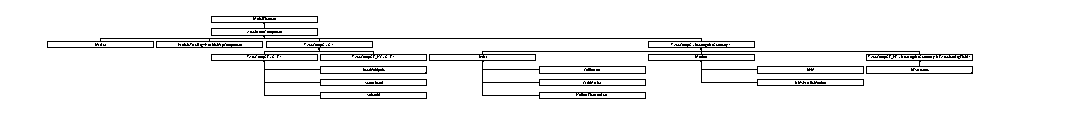
\includegraphics[height=1.102672cm]{classAcceleratorComponent}
\end{center}
\end{figure}
\subsection*{Public Member Functions}
\begin{DoxyCompactItemize}
\item 
virtual int \hyperlink{classAcceleratorComponent_abd1490171ac9af6004d3da01fb3b95fb}{Get\+Index} () const
\item 
double \hyperlink{classAcceleratorComponent_a2922c29d1002d92dc6ecad4a64e5f61e}{Get\+Length} () const
\item 
const \hyperlink{classAcceleratorGeometry}{Accelerator\+Geometry} $\ast$ \hyperlink{classAcceleratorComponent_ac75cb2f0dca9d9ccd2d824a0686bb348}{Get\+Geometry} () const
\item 
const \hyperlink{classEMField}{E\+M\+Field} $\ast$ \hyperlink{classAcceleratorComponent_ae9b86c05ea3b351d5e69683db6cde3b6}{Get\+E\+M\+Field} () const
\item 
\hyperlink{classAperture}{Aperture} $\ast$ \hyperlink{classAcceleratorComponent_aad8b580f5a871205af01c42b6090518f}{Get\+Aperture} () const
\item 
void \hyperlink{classAcceleratorComponent_a5f1b3a0d7bb1b97730f7d7f1e2c968b0}{Set\+Aperture} (\hyperlink{classAperture}{Aperture} $\ast$ap)
\item 
\hyperlink{classWakePotentials}{Wake\+Potentials} $\ast$ \hyperlink{classAcceleratorComponent_a167e52a18f62c9ceffd62ed0c3c079cd}{Get\+Wake\+Potentials} () const
\item 
void \hyperlink{classAcceleratorComponent_a9f9eb01e2e118e1d1f639bbedf0b45ae}{Set\+Wake\+Potentials} (\hyperlink{classWakePotentials}{Wake\+Potentials} $\ast$wp)
\item 
virtual void \hyperlink{classAcceleratorComponent_ab897c54689ac946f40c3ad0716ddd4bb}{Prepare\+Tracker} (\hyperlink{classComponentTracker}{Component\+Tracker} \&a\+Tracker)
\item 
virtual void \hyperlink{classAcceleratorComponent_a8bf0d39b56578ca99f286ca1504b9072}{Rotate\+Y180} ()=0
\item 
void \hyperlink{classAcceleratorComponent_ad3014eb3d45b9991fbd6e4a01137355d}{Set\+Beamline\+Index} (size\+\_\+t n)
\item 
size\+\_\+t \hyperlink{classAcceleratorComponent_a89496aa0510c3227cb3599beaf4967cb}{Get\+Beamline\+Index} () const
\item 
\mbox{\Hypertarget{classAcceleratorComponent_aa69f283744b32db0cff9add563d20a38}\label{classAcceleratorComponent_aa69f283744b32db0cff9add563d20a38}} 
void {\bfseries Append\+Beamline\+Indecies} (std\+::vector$<$ size\+\_\+t $>$ \&) const
\item 
void \hyperlink{classAcceleratorComponent_afab772327a61defbc42a91254b79457c}{Set\+Component\+Lattice\+Position} (double \hyperlink{classAcceleratorComponent_a379d5d0bc151e90328e834f520707c7e}{position})
\item 
double \hyperlink{classAcceleratorComponent_a8283a65382ca795b19448448abba245a}{Get\+Component\+Lattice\+Position} () const
\item 
void \hyperlink{classAcceleratorComponent_a83dc19ee2dae64632cc770e6937828bc}{Set\+Coll\+ID} (int n)
\item 
int \hyperlink{classAcceleratorComponent_a6454158847b9cd68e5b9b0272aa19ecd}{Get\+Coll\+ID} () const
\end{DoxyCompactItemize}
\subsection*{Static Public Member Functions}
\begin{DoxyCompactItemize}
\item 
static int \hyperlink{classAcceleratorComponent_a270378decf9c9b7aea618d11d971170f}{Total\+Component\+Number} ()
\end{DoxyCompactItemize}
\subsection*{Static Public Attributes}
\begin{DoxyCompactItemize}
\item 
static const int \hyperlink{classAcceleratorComponent_ad1c205fd2524942f308ac39e37a7d1be}{ID} = \hyperlink{classAcceleratorComponent_aa7ad4d39e1a488b705983842ed1ac784}{Unique\+Index}()
\end{DoxyCompactItemize}
\subsection*{Protected Member Functions}
\begin{DoxyCompactItemize}
\item 
\hyperlink{classAcceleratorComponent_a2027878fd5cd445eea76291f7b33ae29}{Accelerator\+Component} (const string \&a\+Name=string())
\item 
\hyperlink{classAcceleratorComponent_af7b94670ca7939aedc18e10e9cbfadcb}{Accelerator\+Component} (const string \&a\+Name, \hyperlink{classAcceleratorGeometry}{Accelerator\+Geometry} $\ast$a\+Geom, \hyperlink{classEMField}{E\+M\+Field} $\ast$a\+Field)
\end{DoxyCompactItemize}
\subsection*{Static Protected Member Functions}
\begin{DoxyCompactItemize}
\item 
static int \hyperlink{classAcceleratorComponent_aa7ad4d39e1a488b705983842ed1ac784}{Unique\+Index} ()
\end{DoxyCompactItemize}
\subsection*{Protected Attributes}
\begin{DoxyCompactItemize}
\item 
\hyperlink{classEMField}{E\+M\+Field} $\ast$ \hyperlink{classAcceleratorComponent_a52505c3dfbebf65c38e4de96d72c7718}{its\+Field}
\item 
\hyperlink{classAcceleratorGeometry}{Accelerator\+Geometry} $\ast$ \hyperlink{classAcceleratorComponent_acb1728d9dcd2234fef5b9a6d529db347}{its\+Geometry}
\item 
\hyperlink{classAperture}{Aperture} $\ast$ \hyperlink{classAcceleratorComponent_a776332766062c4e9342ef06d8ba0b45f}{its\+Aperture}
\item 
\hyperlink{classWakePotentials}{Wake\+Potentials} $\ast$ \hyperlink{classAcceleratorComponent_ad1c133d85754bbdc05d72471d9b34ee6}{its\+Wakes}
\item 
double \hyperlink{classAcceleratorComponent_a379d5d0bc151e90328e834f520707c7e}{position}
\item 
size\+\_\+t \hyperlink{classAcceleratorComponent_a73212fc2b6e9f0f71eca5cd633bd5d2f}{blI}
\item 
int \hyperlink{classAcceleratorComponent_a19b829780a5667b311e760329088b9db}{Coll\+\_\+\+ID}
\end{DoxyCompactItemize}


\subsection{Detailed Description}
An \hyperlink{classAcceleratorComponent}{Accelerator\+Component} represents any component which can be placed in an accelerator lattice. Typically, a lattice model is constructed as an ordered sequence of Accelerator\+Components. Accelerator\+Components can be associated with a geometry (an \hyperlink{classAcceleratorGeometry}{Accelerator\+Geometry} object) and a em field (an \hyperlink{classEMField}{E\+M\+Field} Region object), which when taken together uniquely define the field properties for the component. Component \char`\"{}tracking\char`\"{} is supported via the funtion Prepare\+Tracker(\+Tracker\&), which sets up a Tracker object to track the component. 

\subsection{Constructor \& Destructor Documentation}
\mbox{\Hypertarget{classAcceleratorComponent_a2027878fd5cd445eea76291f7b33ae29}\label{classAcceleratorComponent_a2027878fd5cd445eea76291f7b33ae29}} 
\index{Accelerator\+Component@{Accelerator\+Component}!Accelerator\+Component@{Accelerator\+Component}}
\index{Accelerator\+Component@{Accelerator\+Component}!Accelerator\+Component@{Accelerator\+Component}}
\subsubsection{\texorpdfstring{Accelerator\+Component()}{AcceleratorComponent()}\hspace{0.1cm}{\footnotesize\ttfamily [1/2]}}
{\footnotesize\ttfamily Accelerator\+Component\+::\+Accelerator\+Component (\begin{DoxyParamCaption}\item[{const string \&}]{a\+Name = {\ttfamily string()} }\end{DoxyParamCaption})\hspace{0.3cm}{\ttfamily [inline]}, {\ttfamily [explicit]}, {\ttfamily [protected]}}

Protected constructors used by derived classes. 
\begin{DoxyParams}[1]{Parameters}
\mbox{\tt in}  & {\em a\+Name} & The name of the \hyperlink{classAcceleratorComponent}{Accelerator\+Component} \\
\hline
\end{DoxyParams}
\mbox{\Hypertarget{classAcceleratorComponent_af7b94670ca7939aedc18e10e9cbfadcb}\label{classAcceleratorComponent_af7b94670ca7939aedc18e10e9cbfadcb}} 
\index{Accelerator\+Component@{Accelerator\+Component}!Accelerator\+Component@{Accelerator\+Component}}
\index{Accelerator\+Component@{Accelerator\+Component}!Accelerator\+Component@{Accelerator\+Component}}
\subsubsection{\texorpdfstring{Accelerator\+Component()}{AcceleratorComponent()}\hspace{0.1cm}{\footnotesize\ttfamily [2/2]}}
{\footnotesize\ttfamily Accelerator\+Component\+::\+Accelerator\+Component (\begin{DoxyParamCaption}\item[{const string \&}]{a\+Name,  }\item[{\hyperlink{classAcceleratorGeometry}{Accelerator\+Geometry} $\ast$}]{a\+Geom,  }\item[{\hyperlink{classEMField}{E\+M\+Field} $\ast$}]{a\+Field }\end{DoxyParamCaption})\hspace{0.3cm}{\ttfamily [inline]}, {\ttfamily [protected]}}

Protected constructors used by derived classes. 
\begin{DoxyParams}[1]{Parameters}
\mbox{\tt in}  & {\em a\+Name} & The name of the \hyperlink{classAcceleratorComponent}{Accelerator\+Component} \\
\hline
\mbox{\tt in}  & {\em a\+Geom} & The \hyperlink{classAcceleratorGeometry}{Accelerator\+Geometry} of the \hyperlink{classAcceleratorComponent}{Accelerator\+Component} \\
\hline
\mbox{\tt in}  & {\em a\+Field} & The \hyperlink{classEMField}{E\+M\+Field} of the \hyperlink{classAcceleratorComponent}{Accelerator\+Component} \\
\hline
\end{DoxyParams}


\subsection{Member Function Documentation}
\mbox{\Hypertarget{classAcceleratorComponent_aad8b580f5a871205af01c42b6090518f}\label{classAcceleratorComponent_aad8b580f5a871205af01c42b6090518f}} 
\index{Accelerator\+Component@{Accelerator\+Component}!Get\+Aperture@{Get\+Aperture}}
\index{Get\+Aperture@{Get\+Aperture}!Accelerator\+Component@{Accelerator\+Component}}
\subsubsection{\texorpdfstring{Get\+Aperture()}{GetAperture()}}
{\footnotesize\ttfamily \hyperlink{classAperture}{Aperture} $\ast$ Accelerator\+Component\+::\+Get\+Aperture (\begin{DoxyParamCaption}{ }\end{DoxyParamCaption}) const\hspace{0.3cm}{\ttfamily [inline]}}

Returns a pointer to the aperture of this element. \begin{DoxyReturn}{Returns}
The \hyperlink{classAperture}{Aperture} associated with this element. 
\end{DoxyReturn}
\mbox{\Hypertarget{classAcceleratorComponent_a89496aa0510c3227cb3599beaf4967cb}\label{classAcceleratorComponent_a89496aa0510c3227cb3599beaf4967cb}} 
\index{Accelerator\+Component@{Accelerator\+Component}!Get\+Beamline\+Index@{Get\+Beamline\+Index}}
\index{Get\+Beamline\+Index@{Get\+Beamline\+Index}!Accelerator\+Component@{Accelerator\+Component}}
\subsubsection{\texorpdfstring{Get\+Beamline\+Index()}{GetBeamlineIndex()}}
{\footnotesize\ttfamily size\+\_\+t Accelerator\+Component\+::\+Get\+Beamline\+Index (\begin{DoxyParamCaption}{ }\end{DoxyParamCaption}) const\hspace{0.3cm}{\ttfamily [inline]}}

Get the unique beamline index for this frame. \begin{DoxyReturn}{Returns}
A size\+\_\+t containing the unique beamline index. 
\end{DoxyReturn}
\mbox{\Hypertarget{classAcceleratorComponent_a6454158847b9cd68e5b9b0272aa19ecd}\label{classAcceleratorComponent_a6454158847b9cd68e5b9b0272aa19ecd}} 
\index{Accelerator\+Component@{Accelerator\+Component}!Get\+Coll\+ID@{Get\+Coll\+ID}}
\index{Get\+Coll\+ID@{Get\+Coll\+ID}!Accelerator\+Component@{Accelerator\+Component}}
\subsubsection{\texorpdfstring{Get\+Coll\+I\+D()}{GetCollID()}}
{\footnotesize\ttfamily int Accelerator\+Component\+::\+Get\+Coll\+ID (\begin{DoxyParamCaption}{ }\end{DoxyParamCaption}) const\hspace{0.3cm}{\ttfamily [inline]}}

Get the \hyperlink{classCollimator}{Collimator} ID. \begin{DoxyReturn}{Returns}
An integer containing the \hyperlink{classCollimator}{Collimator} ID. 
\end{DoxyReturn}
\mbox{\Hypertarget{classAcceleratorComponent_a8283a65382ca795b19448448abba245a}\label{classAcceleratorComponent_a8283a65382ca795b19448448abba245a}} 
\index{Accelerator\+Component@{Accelerator\+Component}!Get\+Component\+Lattice\+Position@{Get\+Component\+Lattice\+Position}}
\index{Get\+Component\+Lattice\+Position@{Get\+Component\+Lattice\+Position}!Accelerator\+Component@{Accelerator\+Component}}
\subsubsection{\texorpdfstring{Get\+Component\+Lattice\+Position()}{GetComponentLatticePosition()}}
{\footnotesize\ttfamily double Accelerator\+Component\+::\+Get\+Component\+Lattice\+Position (\begin{DoxyParamCaption}{ }\end{DoxyParamCaption}) const\hspace{0.3cm}{\ttfamily [inline]}}

Get the distance from the start of the lattice to the S\+T\+A\+RT of the element. \begin{DoxyReturn}{Returns}
A double containing the position of the start of the lattice element. 
\end{DoxyReturn}
\mbox{\Hypertarget{classAcceleratorComponent_ae9b86c05ea3b351d5e69683db6cde3b6}\label{classAcceleratorComponent_ae9b86c05ea3b351d5e69683db6cde3b6}} 
\index{Accelerator\+Component@{Accelerator\+Component}!Get\+E\+M\+Field@{Get\+E\+M\+Field}}
\index{Get\+E\+M\+Field@{Get\+E\+M\+Field}!Accelerator\+Component@{Accelerator\+Component}}
\subsubsection{\texorpdfstring{Get\+E\+M\+Field()}{GetEMField()}}
{\footnotesize\ttfamily const \hyperlink{classEMField}{E\+M\+Field} $\ast$ Accelerator\+Component\+::\+Get\+E\+M\+Field (\begin{DoxyParamCaption}{ }\end{DoxyParamCaption}) const\hspace{0.3cm}{\ttfamily [inline]}}

Returns a pointer to this components field. A nullptr is returned if the component has no field. \begin{DoxyReturn}{Returns}
The \hyperlink{classEMField}{E\+M\+Field} associated with this element. 
\end{DoxyReturn}
\mbox{\Hypertarget{classAcceleratorComponent_ac75cb2f0dca9d9ccd2d824a0686bb348}\label{classAcceleratorComponent_ac75cb2f0dca9d9ccd2d824a0686bb348}} 
\index{Accelerator\+Component@{Accelerator\+Component}!Get\+Geometry@{Get\+Geometry}}
\index{Get\+Geometry@{Get\+Geometry}!Accelerator\+Component@{Accelerator\+Component}}
\subsubsection{\texorpdfstring{Get\+Geometry()}{GetGeometry()}}
{\footnotesize\ttfamily const \hyperlink{classAcceleratorGeometry}{Accelerator\+Geometry} $\ast$ Accelerator\+Component\+::\+Get\+Geometry (\begin{DoxyParamCaption}{ }\end{DoxyParamCaption}) const\hspace{0.3cm}{\ttfamily [inline]}}

Returns a pointer to the this components geometry. Returns a nullptr if no geometry is associated with this component. \begin{DoxyReturn}{Returns}
The \hyperlink{classAcceleratorGeometry}{Accelerator\+Geometry} associated with this element. 
\end{DoxyReturn}
\mbox{\Hypertarget{classAcceleratorComponent_abd1490171ac9af6004d3da01fb3b95fb}\label{classAcceleratorComponent_abd1490171ac9af6004d3da01fb3b95fb}} 
\index{Accelerator\+Component@{Accelerator\+Component}!Get\+Index@{Get\+Index}}
\index{Get\+Index@{Get\+Index}!Accelerator\+Component@{Accelerator\+Component}}
\subsubsection{\texorpdfstring{Get\+Index()}{GetIndex()}}
{\footnotesize\ttfamily int Accelerator\+Component\+::\+Get\+Index (\begin{DoxyParamCaption}{ }\end{DoxyParamCaption}) const\hspace{0.3cm}{\ttfamily [virtual]}}

Returns the unique index for this class of accelerator components. \begin{DoxyReturn}{Returns}
An integer containing the unique index for this \hyperlink{classAcceleratorComponent}{Accelerator\+Component} type. 
\end{DoxyReturn}


Reimplemented in \hyperlink{classDecapole_ac34dc3e11924c94ff4464cc0ca5ddf68}{Decapole}, \hyperlink{classSkewSextupole_a8dbbf55904005b051ad5d84a9140ab10}{Skew\+Sextupole}, \hyperlink{classOctupole_acf28f59d4bb7f7ad6729e23902915d2b}{Octupole}, \hyperlink{classSectorBend_a1af1ee7a97aa40bc6def14dec661eb3e}{Sector\+Bend}, \hyperlink{classSkewQuadrupole_aa3fb2801ec77a1d9d4d7a4d603c2b767}{Skew\+Quadrupole}, \hyperlink{classBPM_acaf99f021f92252962f2fbcbc24a2679}{B\+PM}, \hyperlink{classSextupole_ab86d63dda91c41c870c89069724681a2}{Sextupole}, \hyperlink{classRMSProfileMonitor_a87a98fa994d96c393a91500320242942}{R\+M\+S\+Profile\+Monitor}, \hyperlink{classMonitor_a38297eb50d06dd56201f2b48d92aa789}{Monitor}, \hyperlink{classCollimator_a158a9d8999d55a27efe4e56e5af8b56a}{Collimator}, \hyperlink{classSolenoid_a6aa64b57e6de710c77242d5e29a6ed8e}{Solenoid}, \hyperlink{classQuadrupole_a39b9e323df34c8db56f6daaaa112cf06}{Quadrupole}, \hyperlink{classParticleTracking_1_1ParticleMapComponent_a7fbbdf569b4535569771f5fc19fc0c76}{Particle\+Tracking\+::\+Particle\+Map\+Component}, \hyperlink{classYCor_a7e13236734c9ea7f52ecc2ee27523c4f}{Y\+Cor}, \hyperlink{classRectMultipole_a9bc789b2a193e341aab8bbd47a0e3ad4}{Rect\+Multipole}, \hyperlink{classTransverseRFStructure_ab19fe781495285c2b088da81fe3ccff0}{Transverse\+R\+F\+Structure}, \hyperlink{classMarker_a3453b35526a601d4c97d689b61f73454}{Marker}, \hyperlink{classDrift_a19bc19d48348912f8693e3ebbf9e92f2}{Drift}, \hyperlink{classTWRFStructure_a5a8ac2ad58e94158e840c5d296fbb53c}{T\+W\+R\+F\+Structure}, \hyperlink{classHollowElectronLens_a87c06909a695e81cb1abc546019e4e40}{Hollow\+Electron\+Lens}, \hyperlink{classXCor_abc1f1ab53804904384d6fadfcbaba5bb}{X\+Cor}, \hyperlink{classCrabMarker_ae8678c41613db9792f84faf3feb88f2b}{Crab\+Marker}, and \hyperlink{classSWRFStructure_aad7467d215cafd843e9a8ad551307ce2}{S\+W\+R\+F\+Structure}.

\mbox{\Hypertarget{classAcceleratorComponent_a2922c29d1002d92dc6ecad4a64e5f61e}\label{classAcceleratorComponent_a2922c29d1002d92dc6ecad4a64e5f61e}} 
\index{Accelerator\+Component@{Accelerator\+Component}!Get\+Length@{Get\+Length}}
\index{Get\+Length@{Get\+Length}!Accelerator\+Component@{Accelerator\+Component}}
\subsubsection{\texorpdfstring{Get\+Length()}{GetLength()}}
{\footnotesize\ttfamily double Accelerator\+Component\+::\+Get\+Length (\begin{DoxyParamCaption}{ }\end{DoxyParamCaption}) const}

Returns the geometry length of the component. \begin{DoxyReturn}{Returns}
A double containing the length of this component. 
\end{DoxyReturn}
\mbox{\Hypertarget{classAcceleratorComponent_a167e52a18f62c9ceffd62ed0c3c079cd}\label{classAcceleratorComponent_a167e52a18f62c9ceffd62ed0c3c079cd}} 
\index{Accelerator\+Component@{Accelerator\+Component}!Get\+Wake\+Potentials@{Get\+Wake\+Potentials}}
\index{Get\+Wake\+Potentials@{Get\+Wake\+Potentials}!Accelerator\+Component@{Accelerator\+Component}}
\subsubsection{\texorpdfstring{Get\+Wake\+Potentials()}{GetWakePotentials()}}
{\footnotesize\ttfamily \hyperlink{classWakePotentials}{Wake\+Potentials} $\ast$ Accelerator\+Component\+::\+Get\+Wake\+Potentials (\begin{DoxyParamCaption}{ }\end{DoxyParamCaption}) const\hspace{0.3cm}{\ttfamily [inline]}}

Returns the wake potentials associated with this element. \begin{DoxyReturn}{Returns}
The \hyperlink{classWakePotentials}{Wake\+Potentials} associated with this element. 
\end{DoxyReturn}
\mbox{\Hypertarget{classAcceleratorComponent_ab897c54689ac946f40c3ad0716ddd4bb}\label{classAcceleratorComponent_ab897c54689ac946f40c3ad0716ddd4bb}} 
\index{Accelerator\+Component@{Accelerator\+Component}!Prepare\+Tracker@{Prepare\+Tracker}}
\index{Prepare\+Tracker@{Prepare\+Tracker}!Accelerator\+Component@{Accelerator\+Component}}
\subsubsection{\texorpdfstring{Prepare\+Tracker()}{PrepareTracker()}}
{\footnotesize\ttfamily void Accelerator\+Component\+::\+Prepare\+Tracker (\begin{DoxyParamCaption}\item[{\hyperlink{classComponentTracker}{Component\+Tracker} \&}]{a\+Tracker }\end{DoxyParamCaption})\hspace{0.3cm}{\ttfamily [virtual]}}

Primary tracking interface. Prepares the specified Tracker object for tracking this component. 
\begin{DoxyParams}[1]{Parameters}
\mbox{\tt in,out}  & {\em a\+Tracker} & The tracker to prepare. \\
\hline
\end{DoxyParams}


Reimplemented in \hyperlink{classDecapole_a7fd7331bfbc39982539f8077afef2e6e}{Decapole}, \hyperlink{classSkewSextupole_a8700a80f9f1863d5f6966cf0827ed342}{Skew\+Sextupole}, \hyperlink{classSectorBend_a1278a47ce282b1229909304ac853fd22}{Sector\+Bend}, \hyperlink{classOctupole_a646ac61a3ef6a66e987df0364d8bb465}{Octupole}, \hyperlink{classSkewQuadrupole_ac277fd65922256a16c1d2774254c09d2}{Skew\+Quadrupole}, \hyperlink{classBPM_a3f0db54eff4f4e95fc2dd81728ea8759}{B\+PM}, \hyperlink{classRMSProfileMonitor_ae5c6ecda857727f6ac78da99b08c88c1}{R\+M\+S\+Profile\+Monitor}, \hyperlink{classSextupole_a7059ddac1812040330950de346e22f48}{Sextupole}, \hyperlink{classMonitor_a8d5e3ab0d68f89a51aabdcde2b01977a}{Monitor}, \hyperlink{classCollimator_acbcf691bfcf53d652d14b9381c711fe7}{Collimator}, \hyperlink{classParticleTracking_1_1ParticleMapComponent_a3490b4f7e961c402ce7eb42ab4e080d7}{Particle\+Tracking\+::\+Particle\+Map\+Component}, \hyperlink{classSolenoid_a565c5334191f0c4b45b053144db29609}{Solenoid}, \hyperlink{classYCor_a6d5d11f3128222ae114d250a2f7d62bb}{Y\+Cor}, \hyperlink{classQuadrupole_aa0160bdc8c7be3d48e400a9698907b15}{Quadrupole}, \hyperlink{classRectMultipole_a2626d08254eee03cffb73abb20a9381a}{Rect\+Multipole}, \hyperlink{classTransverseRFStructure_aa06fabec5aff45f5ac71c5a29f70ca3c}{Transverse\+R\+F\+Structure}, \hyperlink{classXCor_abd5e017ea4191ee86f141d72979f90d2}{X\+Cor}, \hyperlink{classDrift_a9f3925549a0c7c99b39a1abea8546642}{Drift}, \hyperlink{classTWRFStructure_aed3f451bc33edf90177d75c5e53d94af}{T\+W\+R\+F\+Structure}, \hyperlink{classHollowElectronLens_a86e8e69936f636a5d3fa0675e0434bf4}{Hollow\+Electron\+Lens}, \hyperlink{classCrabMarker_ab29822625603a198dc7623979ed1bb3b}{Crab\+Marker}, \hyperlink{classSWRFStructure_a94055441f2ca53c2ccf20e7a07c502b8}{S\+W\+R\+F\+Structure}, and \hyperlink{classMarker_a3910ebbb39ce13360e4dd53897c490ce}{Marker}.

\mbox{\Hypertarget{classAcceleratorComponent_a8bf0d39b56578ca99f286ca1504b9072}\label{classAcceleratorComponent_a8bf0d39b56578ca99f286ca1504b9072}} 
\index{Accelerator\+Component@{Accelerator\+Component}!Rotate\+Y180@{Rotate\+Y180}}
\index{Rotate\+Y180@{Rotate\+Y180}!Accelerator\+Component@{Accelerator\+Component}}
\subsubsection{\texorpdfstring{Rotate\+Y180()}{RotateY180()}}
{\footnotesize\ttfamily virtual void Accelerator\+Component\+::\+Rotate\+Y180 (\begin{DoxyParamCaption}{ }\end{DoxyParamCaption})\hspace{0.3cm}{\ttfamily [pure virtual]}}

Rotates the component 180 degrees about its local Y axis. 

Implemented in \hyperlink{classSectorBend_abd8059191bd4c947320b7fe5f6736e95}{Sector\+Bend}, \hyperlink{classCollimator_a89d782779f8e57af28eeb963078bbf20}{Collimator}, \hyperlink{classParticleTracking_1_1ParticleMapComponent_a32c2b78fc4688e14006f906d5e321d10}{Particle\+Tracking\+::\+Particle\+Map\+Component}, \hyperlink{classMonitor_ad4af2f46ca124bf0c958eca70a2c2769}{Monitor}, \hyperlink{classRectMultipole_afa249ac1d4f3b6c8c1171e5586731ffd}{Rect\+Multipole}, \hyperlink{classSolenoid_aff80a21647e92b9810f2058d9e8540b2}{Solenoid}, \hyperlink{classTransverseRFStructure_a1b016853604d6d2f1c21af600ff52fe0}{Transverse\+R\+F\+Structure}, \hyperlink{classMarker_aa1e927fe0a2eea626759daec624c97f3}{Marker}, \hyperlink{classDrift_abf387eddfcabfc81b186080f6301ce60}{Drift}, \hyperlink{classTWRFStructure_a04893d600099a41642de0634013c5091}{T\+W\+R\+F\+Structure}, \hyperlink{classHollowElectronLens_a8e806750ac6f8129d3be4a089303da36}{Hollow\+Electron\+Lens}, \hyperlink{classCrabMarker_a4b60620517f65b4e1f557300a3dbe89b}{Crab\+Marker}, and \hyperlink{classSWRFStructure_a886ea9cbbef4255f784f440be7c45a91}{S\+W\+R\+F\+Structure}.

\mbox{\Hypertarget{classAcceleratorComponent_a5f1b3a0d7bb1b97730f7d7f1e2c968b0}\label{classAcceleratorComponent_a5f1b3a0d7bb1b97730f7d7f1e2c968b0}} 
\index{Accelerator\+Component@{Accelerator\+Component}!Set\+Aperture@{Set\+Aperture}}
\index{Set\+Aperture@{Set\+Aperture}!Accelerator\+Component@{Accelerator\+Component}}
\subsubsection{\texorpdfstring{Set\+Aperture()}{SetAperture()}}
{\footnotesize\ttfamily void Accelerator\+Component\+::\+Set\+Aperture (\begin{DoxyParamCaption}\item[{\hyperlink{classAperture}{Aperture} $\ast$}]{ap }\end{DoxyParamCaption})\hspace{0.3cm}{\ttfamily [inline]}}

Sets the aperture of this element 
\begin{DoxyParams}[1]{Parameters}
\mbox{\tt in}  & {\em ap} & A pointer to an \hyperlink{classAperture}{Aperture} class to associate with this component \\
\hline
\end{DoxyParams}
\mbox{\Hypertarget{classAcceleratorComponent_ad3014eb3d45b9991fbd6e4a01137355d}\label{classAcceleratorComponent_ad3014eb3d45b9991fbd6e4a01137355d}} 
\index{Accelerator\+Component@{Accelerator\+Component}!Set\+Beamline\+Index@{Set\+Beamline\+Index}}
\index{Set\+Beamline\+Index@{Set\+Beamline\+Index}!Accelerator\+Component@{Accelerator\+Component}}
\subsubsection{\texorpdfstring{Set\+Beamline\+Index()}{SetBeamlineIndex()}}
{\footnotesize\ttfamily void Accelerator\+Component\+::\+Set\+Beamline\+Index (\begin{DoxyParamCaption}\item[{size\+\_\+t}]{n }\end{DoxyParamCaption})\hspace{0.3cm}{\ttfamily [inline]}}

Set the uniques beamline index for this frame. 
\begin{DoxyParams}[1]{Parameters}
\mbox{\tt in}  & {\em n} & The beamline index. \\
\hline
\end{DoxyParams}
\mbox{\Hypertarget{classAcceleratorComponent_a83dc19ee2dae64632cc770e6937828bc}\label{classAcceleratorComponent_a83dc19ee2dae64632cc770e6937828bc}} 
\index{Accelerator\+Component@{Accelerator\+Component}!Set\+Coll\+ID@{Set\+Coll\+ID}}
\index{Set\+Coll\+ID@{Set\+Coll\+ID}!Accelerator\+Component@{Accelerator\+Component}}
\subsubsection{\texorpdfstring{Set\+Coll\+I\+D()}{SetCollID()}}
{\footnotesize\ttfamily void Accelerator\+Component\+::\+Set\+Coll\+ID (\begin{DoxyParamCaption}\item[{int}]{n }\end{DoxyParamCaption})\hspace{0.3cm}{\ttfamily [inline]}}

\hyperlink{classCollimator}{Collimator} ID for F\+L\+U\+KA output A\+V+\+HR 09.\+11.\+15 N.\+B. These values can only be set or got in \hyperlink{classCollimator}{Collimator}. 
\begin{DoxyParams}[1]{Parameters}
\mbox{\tt in}  & {\em n} & The value of the \hyperlink{classCollimator}{Collimator} ID to set. \\
\hline
\end{DoxyParams}
\mbox{\Hypertarget{classAcceleratorComponent_afab772327a61defbc42a91254b79457c}\label{classAcceleratorComponent_afab772327a61defbc42a91254b79457c}} 
\index{Accelerator\+Component@{Accelerator\+Component}!Set\+Component\+Lattice\+Position@{Set\+Component\+Lattice\+Position}}
\index{Set\+Component\+Lattice\+Position@{Set\+Component\+Lattice\+Position}!Accelerator\+Component@{Accelerator\+Component}}
\subsubsection{\texorpdfstring{Set\+Component\+Lattice\+Position()}{SetComponentLatticePosition()}}
{\footnotesize\ttfamily void Accelerator\+Component\+::\+Set\+Component\+Lattice\+Position (\begin{DoxyParamCaption}\item[{double}]{position }\end{DoxyParamCaption})\hspace{0.3cm}{\ttfamily [inline]}}

Set the distance from the start of the lattice to the S\+T\+A\+RT of the element. 
\begin{DoxyParams}[1]{Parameters}
\mbox{\tt in}  & {\em position} & The position of the start of the lattice element. \\
\hline
\end{DoxyParams}
\mbox{\Hypertarget{classAcceleratorComponent_a9f9eb01e2e118e1d1f639bbedf0b45ae}\label{classAcceleratorComponent_a9f9eb01e2e118e1d1f639bbedf0b45ae}} 
\index{Accelerator\+Component@{Accelerator\+Component}!Set\+Wake\+Potentials@{Set\+Wake\+Potentials}}
\index{Set\+Wake\+Potentials@{Set\+Wake\+Potentials}!Accelerator\+Component@{Accelerator\+Component}}
\subsubsection{\texorpdfstring{Set\+Wake\+Potentials()}{SetWakePotentials()}}
{\footnotesize\ttfamily void Accelerator\+Component\+::\+Set\+Wake\+Potentials (\begin{DoxyParamCaption}\item[{\hyperlink{classWakePotentials}{Wake\+Potentials} $\ast$}]{wp }\end{DoxyParamCaption})\hspace{0.3cm}{\ttfamily [inline]}}

Sets the wake potentials associated with this cavity. 
\begin{DoxyParams}[1]{Parameters}
\mbox{\tt in}  & {\em wp} & A pointer to a \hyperlink{classWakePotentials}{Wake\+Potentials} class to associate with this component \\
\hline
\end{DoxyParams}
\mbox{\Hypertarget{classAcceleratorComponent_a270378decf9c9b7aea618d11d971170f}\label{classAcceleratorComponent_a270378decf9c9b7aea618d11d971170f}} 
\index{Accelerator\+Component@{Accelerator\+Component}!Total\+Component\+Number@{Total\+Component\+Number}}
\index{Total\+Component\+Number@{Total\+Component\+Number}!Accelerator\+Component@{Accelerator\+Component}}
\subsubsection{\texorpdfstring{Total\+Component\+Number()}{TotalComponentNumber()}}
{\footnotesize\ttfamily int Accelerator\+Component\+::\+Total\+Component\+Number (\begin{DoxyParamCaption}{ }\end{DoxyParamCaption})\hspace{0.3cm}{\ttfamily [inline]}, {\ttfamily [static]}}

Returns the total number of distinct component types in the system. \begin{DoxyReturn}{Returns}
An integer containing the total number of types of element types that exist. 
\end{DoxyReturn}
\mbox{\Hypertarget{classAcceleratorComponent_aa7ad4d39e1a488b705983842ed1ac784}\label{classAcceleratorComponent_aa7ad4d39e1a488b705983842ed1ac784}} 
\index{Accelerator\+Component@{Accelerator\+Component}!Unique\+Index@{Unique\+Index}}
\index{Unique\+Index@{Unique\+Index}!Accelerator\+Component@{Accelerator\+Component}}
\subsubsection{\texorpdfstring{Unique\+Index()}{UniqueIndex()}}
{\footnotesize\ttfamily int Accelerator\+Component\+::\+Unique\+Index (\begin{DoxyParamCaption}{ }\end{DoxyParamCaption})\hspace{0.3cm}{\ttfamily [static]}, {\ttfamily [protected]}}

Used by derived classes to generate a unique index. All derived classes should have a static member ID of type Index\+Type which should be initialised as follows\+:

Index\+Type component\+::\+ID = \hyperlink{classAcceleratorComponent_aa7ad4d39e1a488b705983842ed1ac784}{Unique\+Index()}; 

\subsection{Member Data Documentation}
\mbox{\Hypertarget{classAcceleratorComponent_a73212fc2b6e9f0f71eca5cd633bd5d2f}\label{classAcceleratorComponent_a73212fc2b6e9f0f71eca5cd633bd5d2f}} 
\index{Accelerator\+Component@{Accelerator\+Component}!blI@{blI}}
\index{blI@{blI}!Accelerator\+Component@{Accelerator\+Component}}
\subsubsection{\texorpdfstring{blI}{blI}}
{\footnotesize\ttfamily size\+\_\+t Accelerator\+Component\+::blI\hspace{0.3cm}{\ttfamily [protected]}}

beamline index associated with this component \mbox{\Hypertarget{classAcceleratorComponent_a19b829780a5667b311e760329088b9db}\label{classAcceleratorComponent_a19b829780a5667b311e760329088b9db}} 
\index{Accelerator\+Component@{Accelerator\+Component}!Coll\+\_\+\+ID@{Coll\+\_\+\+ID}}
\index{Coll\+\_\+\+ID@{Coll\+\_\+\+ID}!Accelerator\+Component@{Accelerator\+Component}}
\subsubsection{\texorpdfstring{Coll\+\_\+\+ID}{Coll\_ID}}
{\footnotesize\ttfamily int Accelerator\+Component\+::\+Coll\+\_\+\+ID\hspace{0.3cm}{\ttfamily [protected]}}

\hyperlink{classCollimator}{Collimator} ID for F\+L\+U\+KA output A\+V+\+HR 09.\+11.\+15 N.\+B. These values can only be set or got in \hyperlink{classCollimator}{Collimator} \mbox{\Hypertarget{classAcceleratorComponent_ad1c205fd2524942f308ac39e37a7d1be}\label{classAcceleratorComponent_ad1c205fd2524942f308ac39e37a7d1be}} 
\index{Accelerator\+Component@{Accelerator\+Component}!ID@{ID}}
\index{ID@{ID}!Accelerator\+Component@{Accelerator\+Component}}
\subsubsection{\texorpdfstring{ID}{ID}}
{\footnotesize\ttfamily const int Accelerator\+Component\+::\+ID = \hyperlink{classAcceleratorComponent_aa7ad4d39e1a488b705983842ed1ac784}{Unique\+Index}()\hspace{0.3cm}{\ttfamily [static]}}

Unique index for an Accelerator component. \mbox{\Hypertarget{classAcceleratorComponent_a776332766062c4e9342ef06d8ba0b45f}\label{classAcceleratorComponent_a776332766062c4e9342ef06d8ba0b45f}} 
\index{Accelerator\+Component@{Accelerator\+Component}!its\+Aperture@{its\+Aperture}}
\index{its\+Aperture@{its\+Aperture}!Accelerator\+Component@{Accelerator\+Component}}
\subsubsection{\texorpdfstring{its\+Aperture}{itsAperture}}
{\footnotesize\ttfamily \hyperlink{classAperture}{Aperture}$\ast$ Accelerator\+Component\+::its\+Aperture\hspace{0.3cm}{\ttfamily [protected]}}

A pointer to the \hyperlink{classAperture}{Aperture} for this component \mbox{\Hypertarget{classAcceleratorComponent_a52505c3dfbebf65c38e4de96d72c7718}\label{classAcceleratorComponent_a52505c3dfbebf65c38e4de96d72c7718}} 
\index{Accelerator\+Component@{Accelerator\+Component}!its\+Field@{its\+Field}}
\index{its\+Field@{its\+Field}!Accelerator\+Component@{Accelerator\+Component}}
\subsubsection{\texorpdfstring{its\+Field}{itsField}}
{\footnotesize\ttfamily \hyperlink{classEMField}{E\+M\+Field}$\ast$ Accelerator\+Component\+::its\+Field\hspace{0.3cm}{\ttfamily [protected]}}

A pointer to the Electromagnetic field for this component \mbox{\Hypertarget{classAcceleratorComponent_acb1728d9dcd2234fef5b9a6d529db347}\label{classAcceleratorComponent_acb1728d9dcd2234fef5b9a6d529db347}} 
\index{Accelerator\+Component@{Accelerator\+Component}!its\+Geometry@{its\+Geometry}}
\index{its\+Geometry@{its\+Geometry}!Accelerator\+Component@{Accelerator\+Component}}
\subsubsection{\texorpdfstring{its\+Geometry}{itsGeometry}}
{\footnotesize\ttfamily \hyperlink{classAcceleratorGeometry}{Accelerator\+Geometry}$\ast$ Accelerator\+Component\+::its\+Geometry\hspace{0.3cm}{\ttfamily [protected]}}

A pointer to the geometry for this component \mbox{\Hypertarget{classAcceleratorComponent_ad1c133d85754bbdc05d72471d9b34ee6}\label{classAcceleratorComponent_ad1c133d85754bbdc05d72471d9b34ee6}} 
\index{Accelerator\+Component@{Accelerator\+Component}!its\+Wakes@{its\+Wakes}}
\index{its\+Wakes@{its\+Wakes}!Accelerator\+Component@{Accelerator\+Component}}
\subsubsection{\texorpdfstring{its\+Wakes}{itsWakes}}
{\footnotesize\ttfamily \hyperlink{classWakePotentials}{Wake\+Potentials}$\ast$ Accelerator\+Component\+::its\+Wakes\hspace{0.3cm}{\ttfamily [protected]}}

A pointer to the Wake potentials for this component \mbox{\Hypertarget{classAcceleratorComponent_a379d5d0bc151e90328e834f520707c7e}\label{classAcceleratorComponent_a379d5d0bc151e90328e834f520707c7e}} 
\index{Accelerator\+Component@{Accelerator\+Component}!position@{position}}
\index{position@{position}!Accelerator\+Component@{Accelerator\+Component}}
\subsubsection{\texorpdfstring{position}{position}}
{\footnotesize\ttfamily double Accelerator\+Component\+::position\hspace{0.3cm}{\ttfamily [protected]}}

The position of this element relative to a user defined location (the start of the user generated lattice). 

The documentation for this class was generated from the following files\+:\begin{DoxyCompactItemize}
\item 
/home/fallon/git/merlin-\/cmake/\+Merlin/Accelerator\+Component.\+h\item 
/home/fallon/git/merlin-\/cmake/\+Merlin/Accelerator\+Component.\+cpp\end{DoxyCompactItemize}

\hypertarget{classAcceleratorErrors}{}\section{Accelerator\+Errors Class Reference}
\label{classAcceleratorErrors}\index{Accelerator\+Errors@{Accelerator\+Errors}}


{\ttfamily \#include $<$Accelerator\+Errors.\+h$>$}

\subsection*{Public Member Functions}
\begin{DoxyCompactItemize}
\item 
\hyperlink{classAcceleratorErrors_a7abb6cc331fd2e15b613c494278fc3a7}{Accelerator\+Errors} ()
\item 
void \hyperlink{classAcceleratorErrors_a311e816f0302392322af08a8399cc117}{Set\+Errors} (double xrms=0, double yrms=0, double zrms=0, double meanx=0, double meany=0, double meanz=0)
\item 
void \hyperlink{classAcceleratorErrors_a1f8965c77693446153115e78259c8f31}{Add\+Errors} (double xrms=0, double yrms=0, double zrms=0, double meanx=0, double meany=0, double meanz=0)
\item 
void \hyperlink{classAcceleratorErrors_a75f6bf4af0e2a4a562c246a1a4307315}{Apply\+Shifts} (\hyperlink{classAcceleratorModel_1_1Beamline}{Accelerator\+Model\+::\+Beamline} \&b, const string \&p)
\item 
void \hyperlink{classAcceleratorErrors_af8b9a5703660bc525e53697d50e97fe2}{Apply\+Rotations} (\hyperlink{classAcceleratorModel_1_1Beamline}{Accelerator\+Model\+::\+Beamline} \&b, const string \&p)
\item 
void \hyperlink{classAcceleratorErrors_a39081834644d4132b258749094febd7a}{Report} (ostream $\ast$l)
\end{DoxyCompactItemize}


\subsection{Detailed Description}
A class to apply random normally distributed errors to a beamline. Both shift (transverse and longitudinal) and rotational errors can be generated. \begin{DoxyAuthor}{Author}
Dirk Kruecker 
\end{DoxyAuthor}
\begin{DoxyDate}{Date}
2008-\/12-\/01 
\end{DoxyDate}


\subsection{Constructor \& Destructor Documentation}
\mbox{\Hypertarget{classAcceleratorErrors_a7abb6cc331fd2e15b613c494278fc3a7}\label{classAcceleratorErrors_a7abb6cc331fd2e15b613c494278fc3a7}} 
\index{Accelerator\+Errors@{Accelerator\+Errors}!Accelerator\+Errors@{Accelerator\+Errors}}
\index{Accelerator\+Errors@{Accelerator\+Errors}!Accelerator\+Errors@{Accelerator\+Errors}}
\subsubsection{\texorpdfstring{Accelerator\+Errors()}{AcceleratorErrors()}}
{\footnotesize\ttfamily Accelerator\+Errors\+::\+Accelerator\+Errors (\begin{DoxyParamCaption}{ }\end{DoxyParamCaption})\hspace{0.3cm}{\ttfamily [inline]}}

Constructor 

\subsection{Member Function Documentation}
\mbox{\Hypertarget{classAcceleratorErrors_a1f8965c77693446153115e78259c8f31}\label{classAcceleratorErrors_a1f8965c77693446153115e78259c8f31}} 
\index{Accelerator\+Errors@{Accelerator\+Errors}!Add\+Errors@{Add\+Errors}}
\index{Add\+Errors@{Add\+Errors}!Accelerator\+Errors@{Accelerator\+Errors}}
\subsubsection{\texorpdfstring{Add\+Errors()}{AddErrors()}}
{\footnotesize\ttfamily void Accelerator\+Errors\+::\+Add\+Errors (\begin{DoxyParamCaption}\item[{double}]{xrms = {\ttfamily 0},  }\item[{double}]{yrms = {\ttfamily 0},  }\item[{double}]{zrms = {\ttfamily 0},  }\item[{double}]{meanx = {\ttfamily 0},  }\item[{double}]{meany = {\ttfamily 0},  }\item[{double}]{meanz = {\ttfamily 0} }\end{DoxyParamCaption})\hspace{0.3cm}{\ttfamily [inline]}}

Set the errors to apply to a Beamline. This function does N\+OT clear out any previous \hyperlink{classLatticeFrame}{Lattice\+Frame} movements that have been applied. It will add to any movements that have been applied. \begin{DoxySeeAlso}{See also}
\hyperlink{classAcceleratorErrors_a311e816f0302392322af08a8399cc117}{Set\+Errors} 
\end{DoxySeeAlso}

\begin{DoxyParams}[1]{Parameters}
\mbox{\tt in}  & {\em xrms} & The root mean square value for x errors. \\
\hline
\mbox{\tt in}  & {\em yrms} & The root mean square value for y errors. \\
\hline
\mbox{\tt in}  & {\em zrms} & The root mean square value for z errors. \\
\hline
\mbox{\tt in}  & {\em meanx} & The root mean square value for x errors. \\
\hline
\mbox{\tt in}  & {\em meany} & The root mean square value for y errors. \\
\hline
\mbox{\tt in}  & {\em meanz} & The root mean square value for z errors. \\
\hline
\end{DoxyParams}
\mbox{\Hypertarget{classAcceleratorErrors_af8b9a5703660bc525e53697d50e97fe2}\label{classAcceleratorErrors_af8b9a5703660bc525e53697d50e97fe2}} 
\index{Accelerator\+Errors@{Accelerator\+Errors}!Apply\+Rotations@{Apply\+Rotations}}
\index{Apply\+Rotations@{Apply\+Rotations}!Accelerator\+Errors@{Accelerator\+Errors}}
\subsubsection{\texorpdfstring{Apply\+Rotations()}{ApplyRotations()}}
{\footnotesize\ttfamily void Accelerator\+Errors\+::\+Apply\+Rotations (\begin{DoxyParamCaption}\item[{\hyperlink{classAcceleratorModel_1_1Beamline}{Accelerator\+Model\+::\+Beamline} \&}]{b,  }\item[{const string \&}]{p }\end{DoxyParamCaption})}

Apply the set rotational errors to all elements matching a string pattern to a selected (sub) Beamline. 
\begin{DoxyParams}[1]{Parameters}
\mbox{\tt in}  & {\em b} & The Beamline to apply the rotational errors to. \\
\hline
\mbox{\tt in}  & {\em p} & The string pattern for the names of elements to match for the application of errors. \\
\hline
\end{DoxyParams}
\mbox{\Hypertarget{classAcceleratorErrors_a75f6bf4af0e2a4a562c246a1a4307315}\label{classAcceleratorErrors_a75f6bf4af0e2a4a562c246a1a4307315}} 
\index{Accelerator\+Errors@{Accelerator\+Errors}!Apply\+Shifts@{Apply\+Shifts}}
\index{Apply\+Shifts@{Apply\+Shifts}!Accelerator\+Errors@{Accelerator\+Errors}}
\subsubsection{\texorpdfstring{Apply\+Shifts()}{ApplyShifts()}}
{\footnotesize\ttfamily void Accelerator\+Errors\+::\+Apply\+Shifts (\begin{DoxyParamCaption}\item[{\hyperlink{classAcceleratorModel_1_1Beamline}{Accelerator\+Model\+::\+Beamline} \&}]{b,  }\item[{const string \&}]{p }\end{DoxyParamCaption})}

Apply the set shift errors to all elements matching a string pattern to a selected (sub) Beamline. 
\begin{DoxyParams}[1]{Parameters}
\mbox{\tt in}  & {\em b} & The Beamline to apply the shift errors to. \\
\hline
\mbox{\tt in}  & {\em p} & The string pattern for the names of elements to match for the application of errors. \\
\hline
\end{DoxyParams}
\mbox{\Hypertarget{classAcceleratorErrors_a39081834644d4132b258749094febd7a}\label{classAcceleratorErrors_a39081834644d4132b258749094febd7a}} 
\index{Accelerator\+Errors@{Accelerator\+Errors}!Report@{Report}}
\index{Report@{Report}!Accelerator\+Errors@{Accelerator\+Errors}}
\subsubsection{\texorpdfstring{Report()}{Report()}}
{\footnotesize\ttfamily void Accelerator\+Errors\+::\+Report (\begin{DoxyParamCaption}\item[{ostream $\ast$}]{l }\end{DoxyParamCaption})\hspace{0.3cm}{\ttfamily [inline]}}

Sets the log stream to output logging information to. 
\begin{DoxyParams}[1]{Parameters}
\mbox{\tt in}  & {\em l} & The stream to use for output. \\
\hline
\end{DoxyParams}
\mbox{\Hypertarget{classAcceleratorErrors_a311e816f0302392322af08a8399cc117}\label{classAcceleratorErrors_a311e816f0302392322af08a8399cc117}} 
\index{Accelerator\+Errors@{Accelerator\+Errors}!Set\+Errors@{Set\+Errors}}
\index{Set\+Errors@{Set\+Errors}!Accelerator\+Errors@{Accelerator\+Errors}}
\subsubsection{\texorpdfstring{Set\+Errors()}{SetErrors()}}
{\footnotesize\ttfamily void Accelerator\+Errors\+::\+Set\+Errors (\begin{DoxyParamCaption}\item[{double}]{xrms = {\ttfamily 0},  }\item[{double}]{yrms = {\ttfamily 0},  }\item[{double}]{zrms = {\ttfamily 0},  }\item[{double}]{meanx = {\ttfamily 0},  }\item[{double}]{meany = {\ttfamily 0},  }\item[{double}]{meanz = {\ttfamily 0} }\end{DoxyParamCaption})\hspace{0.3cm}{\ttfamily [inline]}}

Set the errors to apply to a Beamline. This function clears out any previous \hyperlink{classLatticeFrame}{Lattice\+Frame} movements that have been applied. \begin{DoxySeeAlso}{See also}
\hyperlink{classAcceleratorErrors_a1f8965c77693446153115e78259c8f31}{Add\+Errors} 
\end{DoxySeeAlso}

\begin{DoxyParams}[1]{Parameters}
\mbox{\tt in}  & {\em xrms} & The root mean square value for x errors. \\
\hline
\mbox{\tt in}  & {\em yrms} & The root mean square value for y errors. \\
\hline
\mbox{\tt in}  & {\em zrms} & The root mean square value for z errors. \\
\hline
\mbox{\tt in}  & {\em meanx} & The root mean square value for x errors. \\
\hline
\mbox{\tt in}  & {\em meany} & The root mean square value for y errors. \\
\hline
\mbox{\tt in}  & {\em meanz} & The root mean square value for z errors. \\
\hline
\end{DoxyParams}


The documentation for this class was generated from the following files\+:\begin{DoxyCompactItemize}
\item 
/home/fallon/git/merlin-\/cmake/\+Merlin/Accelerator\+Errors.\+h\item 
/home/fallon/git/merlin-\/cmake/\+Merlin/Accelerator\+Errors.\+cpp\end{DoxyCompactItemize}

\hypertarget{classAcceleratorGeometry}{}\section{Accelerator\+Geometry Class Reference}
\label{classAcceleratorGeometry}\index{Accelerator\+Geometry@{Accelerator\+Geometry}}


{\ttfamily \#include $<$Accelerator\+Geometry.\+h$>$}

Inheritance diagram for Accelerator\+Geometry\+:\begin{figure}[H]
\begin{center}
\leavevmode
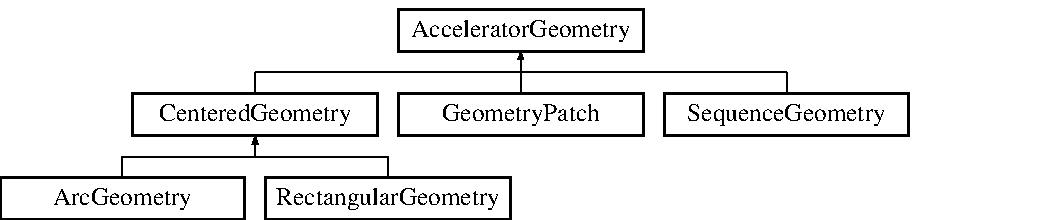
\includegraphics[height=2.957747cm]{classAcceleratorGeometry}
\end{center}
\end{figure}
\subsection*{Classes}
\begin{DoxyCompactItemize}
\item 
class \hyperlink{classAcceleratorGeometry_1_1BeyondExtent}{Beyond\+Extent}
\end{DoxyCompactItemize}
\subsection*{Public Types}
\begin{DoxyCompactItemize}
\item 
enum \hyperlink{classAcceleratorGeometry_a5c1661938176102f235836f5a8be6034}{Boundary\+Plane} \{ {\bfseries entrance}, 
{\bfseries exit}
 \}
\item 
\mbox{\Hypertarget{classAcceleratorGeometry_a8d2b94993161c0b2e4e6488ddd534b7f}\label{classAcceleratorGeometry_a8d2b94993161c0b2e4e6488ddd534b7f}} 
typedef std\+::pair$<$ double, double $>$ {\bfseries Extent}
\end{DoxyCompactItemize}
\subsection*{Public Member Functions}
\begin{DoxyCompactItemize}
\item 
virtual \hyperlink{classAcceleratorGeometry_aff2b5c1086ebcb68c68786e56d7db458}{$\sim$\+Accelerator\+Geometry} ()
\item 
virtual \hyperlink{classTransform3D}{Transform3D} \hyperlink{classAcceleratorGeometry_abf9c17cd1f84ac3e41973c85a65004de}{Get\+Geometry\+Transform} (double s0, double s) const =0
\item 
\hyperlink{classTransform3D}{Transform3D} \hyperlink{classAcceleratorGeometry_a47b2428c2a37fa828940ec35c20a956d}{Get\+Geometry\+Transform} (double s) const
\item 
virtual \hyperlink{classTransform3D}{Transform3D} \hyperlink{classAcceleratorGeometry_af26654f89c4bff1b516d2c6d6bb68871}{Get\+Geometry\+Transform} (\hyperlink{classAcceleratorGeometry_a5c1661938176102f235836f5a8be6034}{Boundary\+Plane} p) const =0
\item 
virtual \hyperlink{classTransform3D}{Transform3D} \hyperlink{classAcceleratorGeometry_a9bffb8262fc3b28195e1e25fbfb2b8ba}{Get\+Total\+Geometry\+Transform} () const
\item 
virtual Extent \hyperlink{classAcceleratorGeometry_a2db830fe927af3c9cba59b8452370bfb}{Get\+Geometry\+Extent} () const =0
\item 
virtual double \hyperlink{classAcceleratorGeometry_abc36f96d542e0d9db592f8e7ee455769}{Get\+Geometry\+Length} () const =0
\end{DoxyCompactItemize}


\subsection{Detailed Description}
Represents a frame of reference for a section of accelerator lattice. An \hyperlink{classAcceleratorGeometry}{Accelerator\+Geometry} can be considered a type of three-\/dimensional space line (R(s)), which is characterised by a single scalar s, the distance along the space line from the origin. Each \hyperlink{classAcceleratorGeometry}{Accelerator\+Geometry} has a specific length which bounds the allowed values of s (with respect to the local geometry origin). At each position s on the geometry, a local rectangular coordinate frame can be uniquely defined, with its origin at the point s, and its z-\/axis tangential to the geometry at s. The orientation of the local x-\/ and y-\/axes are also uniquely determined by the sum of any rotations applied going from the origin to s.

The primary responsibilty for an \hyperlink{classAcceleratorGeometry}{Accelerator\+Geometry} object is to supply transformations between coordinate frames defined on that geometry. 

\subsection{Member Enumeration Documentation}
\mbox{\Hypertarget{classAcceleratorGeometry_a5c1661938176102f235836f5a8be6034}\label{classAcceleratorGeometry_a5c1661938176102f235836f5a8be6034}} 
\index{Accelerator\+Geometry@{Accelerator\+Geometry}!Boundary\+Plane@{Boundary\+Plane}}
\index{Boundary\+Plane@{Boundary\+Plane}!Accelerator\+Geometry@{Accelerator\+Geometry}}
\subsubsection{\texorpdfstring{Boundary\+Plane}{BoundaryPlane}}
{\footnotesize\ttfamily enum \hyperlink{classAcceleratorGeometry_a5c1661938176102f235836f5a8be6034}{Accelerator\+Geometry\+::\+Boundary\+Plane}}

A Boundary\+Plane is the X-\/Y plane (z=0) of the coordinate frame defined at the entrance (start) or exit (end) of the Geometry. 

\subsection{Constructor \& Destructor Documentation}
\mbox{\Hypertarget{classAcceleratorGeometry_aff2b5c1086ebcb68c68786e56d7db458}\label{classAcceleratorGeometry_aff2b5c1086ebcb68c68786e56d7db458}} 
\index{Accelerator\+Geometry@{Accelerator\+Geometry}!````~Accelerator\+Geometry@{$\sim$\+Accelerator\+Geometry}}
\index{````~Accelerator\+Geometry@{$\sim$\+Accelerator\+Geometry}!Accelerator\+Geometry@{Accelerator\+Geometry}}
\subsubsection{\texorpdfstring{$\sim$\+Accelerator\+Geometry()}{~AcceleratorGeometry()}}
{\footnotesize\ttfamily Accelerator\+Geometry\+::$\sim$\+Accelerator\+Geometry (\begin{DoxyParamCaption}{ }\end{DoxyParamCaption})\hspace{0.3cm}{\ttfamily [inline]}, {\ttfamily [virtual]}}

Virtual destructor. 

\subsection{Member Function Documentation}
\mbox{\Hypertarget{classAcceleratorGeometry_a2db830fe927af3c9cba59b8452370bfb}\label{classAcceleratorGeometry_a2db830fe927af3c9cba59b8452370bfb}} 
\index{Accelerator\+Geometry@{Accelerator\+Geometry}!Get\+Geometry\+Extent@{Get\+Geometry\+Extent}}
\index{Get\+Geometry\+Extent@{Get\+Geometry\+Extent}!Accelerator\+Geometry@{Accelerator\+Geometry}}
\subsubsection{\texorpdfstring{Get\+Geometry\+Extent()}{GetGeometryExtent()}}
{\footnotesize\ttfamily virtual Extent Accelerator\+Geometry\+::\+Get\+Geometry\+Extent (\begin{DoxyParamCaption}{ }\end{DoxyParamCaption}) const\hspace{0.3cm}{\ttfamily [pure virtual]}}

Returns the local extent of this geometry. \begin{DoxyReturn}{Returns}
A pair giving the extent of this geometry. 
\end{DoxyReturn}


Implemented in \hyperlink{classGeometryPatch_a814a517dd837f92d7f26628562047cb2}{Geometry\+Patch}, \hyperlink{classSequenceGeometry_a1d904b73570a03e3496dbbd574b8fde0}{Sequence\+Geometry}, and \hyperlink{classCenteredGeometry_abd27afe15472ebd057d0b60f1d531a1a}{Centered\+Geometry}.

\mbox{\Hypertarget{classAcceleratorGeometry_abc36f96d542e0d9db592f8e7ee455769}\label{classAcceleratorGeometry_abc36f96d542e0d9db592f8e7ee455769}} 
\index{Accelerator\+Geometry@{Accelerator\+Geometry}!Get\+Geometry\+Length@{Get\+Geometry\+Length}}
\index{Get\+Geometry\+Length@{Get\+Geometry\+Length}!Accelerator\+Geometry@{Accelerator\+Geometry}}
\subsubsection{\texorpdfstring{Get\+Geometry\+Length()}{GetGeometryLength()}}
{\footnotesize\ttfamily virtual double Accelerator\+Geometry\+::\+Get\+Geometry\+Length (\begin{DoxyParamCaption}{ }\end{DoxyParamCaption}) const\hspace{0.3cm}{\ttfamily [pure virtual]}}

Returns the total arc-\/length of the geometry. \begin{DoxyReturn}{Returns}
A double giving the total length of this geometry. 
\end{DoxyReturn}


Implemented in \hyperlink{classGeometryPatch_ae2d9aef3fc3df96fdf0340124f099997}{Geometry\+Patch}, \hyperlink{classSequenceGeometry_a322e113ebda69e6c42af9415f3c964d9}{Sequence\+Geometry}, and \hyperlink{classCenteredGeometry_afe03a287567dec16f8663f4211f82add}{Centered\+Geometry}.

\mbox{\Hypertarget{classAcceleratorGeometry_abf9c17cd1f84ac3e41973c85a65004de}\label{classAcceleratorGeometry_abf9c17cd1f84ac3e41973c85a65004de}} 
\index{Accelerator\+Geometry@{Accelerator\+Geometry}!Get\+Geometry\+Transform@{Get\+Geometry\+Transform}}
\index{Get\+Geometry\+Transform@{Get\+Geometry\+Transform}!Accelerator\+Geometry@{Accelerator\+Geometry}}
\subsubsection{\texorpdfstring{Get\+Geometry\+Transform()}{GetGeometryTransform()}\hspace{0.1cm}{\footnotesize\ttfamily [1/3]}}
{\footnotesize\ttfamily virtual \hyperlink{classTransform3D}{Transform3D} Accelerator\+Geometry\+::\+Get\+Geometry\+Transform (\begin{DoxyParamCaption}\item[{double}]{s0,  }\item[{double}]{s }\end{DoxyParamCaption}) const\hspace{0.3cm}{\ttfamily [pure virtual]}}

Return the three-\/dimensional transformation from the frame at s0 to the frame at s. s and s0 are in the geometry\textquotesingle{}s s-\/frame, and must be within the geometry extents. 
\begin{DoxyParams}[1]{Parameters}
\mbox{\tt in}  & {\em s0} & The location at which the transform should be evalutated from. \\
\hline
\mbox{\tt in}  & {\em s} & The location at which the transform should be evalutated to. \\
\hline
\end{DoxyParams}

\begin{DoxyExceptions}{Exceptions}
{\em Throws} & a \hyperlink{classAcceleratorGeometry_1_1BeyondExtent}{Beyond\+Extent} exception if the requested s values are outside the geometry extent. \\
\hline
\end{DoxyExceptions}
\begin{DoxyReturn}{Returns}
The 3D transformation from the entrance to the exit of this geometry. 
\end{DoxyReturn}


Implemented in \hyperlink{classArcGeometry_affd534869f6f79b4b271a07b51145b7c}{Arc\+Geometry}, \hyperlink{classSequenceGeometry_a7531d4e915026c4978f12190d6908167}{Sequence\+Geometry}, \hyperlink{classGeometryPatch_ae45360bf4f4a8bad9189eb34bca2a919}{Geometry\+Patch}, and \hyperlink{classRectangularGeometry_a2e25d8cd4902949308ffd031544ca8c9}{Rectangular\+Geometry}.

\mbox{\Hypertarget{classAcceleratorGeometry_a47b2428c2a37fa828940ec35c20a956d}\label{classAcceleratorGeometry_a47b2428c2a37fa828940ec35c20a956d}} 
\index{Accelerator\+Geometry@{Accelerator\+Geometry}!Get\+Geometry\+Transform@{Get\+Geometry\+Transform}}
\index{Get\+Geometry\+Transform@{Get\+Geometry\+Transform}!Accelerator\+Geometry@{Accelerator\+Geometry}}
\subsubsection{\texorpdfstring{Get\+Geometry\+Transform()}{GetGeometryTransform()}\hspace{0.1cm}{\footnotesize\ttfamily [2/3]}}
{\footnotesize\ttfamily \hyperlink{classTransform3D}{Transform3D} Accelerator\+Geometry\+::\+Get\+Geometry\+Transform (\begin{DoxyParamCaption}\item[{double}]{s }\end{DoxyParamCaption}) const\hspace{0.3cm}{\ttfamily [inline]}}

Return the three-\/dimensional transformation from the local origin to the frame at s. s is in the geometry\textquotesingle{}s s-\/frame, and must be within the geometry extents. 
\begin{DoxyParams}[1]{Parameters}
\mbox{\tt in}  & {\em s} & The location at which the transform should be evalutated to. \\
\hline
\end{DoxyParams}

\begin{DoxyExceptions}{Exceptions}
{\em Throws} & a \hyperlink{classAcceleratorGeometry_1_1BeyondExtent}{Beyond\+Extent} exception if the requested s value is outside the geometry extent. \\
\hline
\end{DoxyExceptions}
\begin{DoxyReturn}{Returns}
The 3D transformation from the entrance to the exit of this geometry. 
\end{DoxyReturn}
\mbox{\Hypertarget{classAcceleratorGeometry_af26654f89c4bff1b516d2c6d6bb68871}\label{classAcceleratorGeometry_af26654f89c4bff1b516d2c6d6bb68871}} 
\index{Accelerator\+Geometry@{Accelerator\+Geometry}!Get\+Geometry\+Transform@{Get\+Geometry\+Transform}}
\index{Get\+Geometry\+Transform@{Get\+Geometry\+Transform}!Accelerator\+Geometry@{Accelerator\+Geometry}}
\subsubsection{\texorpdfstring{Get\+Geometry\+Transform()}{GetGeometryTransform()}\hspace{0.1cm}{\footnotesize\ttfamily [3/3]}}
{\footnotesize\ttfamily virtual \hyperlink{classTransform3D}{Transform3D} Accelerator\+Geometry\+::\+Get\+Geometry\+Transform (\begin{DoxyParamCaption}\item[{\hyperlink{classAcceleratorGeometry_a5c1661938176102f235836f5a8be6034}{Boundary\+Plane}}]{p }\end{DoxyParamCaption}) const\hspace{0.3cm}{\ttfamily [pure virtual]}}

Returns the transformation from the geometry origin to the specified boundary plane. 
\begin{DoxyParams}[1]{Parameters}
\mbox{\tt in}  & {\em p} & The chosen Boundary\+Plane \\
\hline
\end{DoxyParams}
\begin{DoxyReturn}{Returns}
The 3D transformation from the geometry origin to a specified boundary plane (extrance or exit). 
\end{DoxyReturn}


Implemented in \hyperlink{classArcGeometry_aaa665b9dba9b879f38cb5e4a97967533}{Arc\+Geometry}, \hyperlink{classSequenceGeometry_a4dc3260e63d8fff7b22d7d7908741b1f}{Sequence\+Geometry}, \hyperlink{classGeometryPatch_a461f15c9a93cc4473463191c9d0f6465}{Geometry\+Patch}, and \hyperlink{classRectangularGeometry_a21891a331a7ac6cb4283d95115c29020}{Rectangular\+Geometry}.

\mbox{\Hypertarget{classAcceleratorGeometry_a9bffb8262fc3b28195e1e25fbfb2b8ba}\label{classAcceleratorGeometry_a9bffb8262fc3b28195e1e25fbfb2b8ba}} 
\index{Accelerator\+Geometry@{Accelerator\+Geometry}!Get\+Total\+Geometry\+Transform@{Get\+Total\+Geometry\+Transform}}
\index{Get\+Total\+Geometry\+Transform@{Get\+Total\+Geometry\+Transform}!Accelerator\+Geometry@{Accelerator\+Geometry}}
\subsubsection{\texorpdfstring{Get\+Total\+Geometry\+Transform()}{GetTotalGeometryTransform()}}
{\footnotesize\ttfamily \hyperlink{classTransform3D}{Transform3D} Accelerator\+Geometry\+::\+Get\+Total\+Geometry\+Transform (\begin{DoxyParamCaption}{ }\end{DoxyParamCaption}) const\hspace{0.3cm}{\ttfamily [virtual]}}

Returns the transformation from the entrance plane frame to the exit plane frame. \begin{DoxyReturn}{Returns}
The 3D transformation from the entrance to the exit of this geometry. 
\end{DoxyReturn}


Reimplemented in \hyperlink{classArcGeometry_aceed7dd7294528003f4bd9f624ef6c9b}{Arc\+Geometry}, \hyperlink{classSequenceGeometry_a8c7221a5186be9cefe0f7fc674447e71}{Sequence\+Geometry}, \hyperlink{classGeometryPatch_a94c4c26b1a43acc6a34b29d00a229d70}{Geometry\+Patch}, and \hyperlink{classRectangularGeometry_a830506a331c8b08def936613ed727c62}{Rectangular\+Geometry}.



The documentation for this class was generated from the following files\+:\begin{DoxyCompactItemize}
\item 
/home/fallon/git/merlin-\/cmake/\+Merlin/Accelerator\+Geometry.\+h\item 
/home/fallon/git/merlin-\/cmake/\+Merlin/Accelerator\+Geometry.\+cpp\end{DoxyCompactItemize}

\hypertarget{classAcceleratorModel}{}\section{Accelerator\+Model Class Reference}
\label{classAcceleratorModel}\index{Accelerator\+Model@{Accelerator\+Model}}
\subsection*{Classes}
\begin{DoxyCompactItemize}
\item 
class \hyperlink{classAcceleratorModel_1_1BadRange}{Bad\+Range}
\item 
class \hyperlink{classAcceleratorModel_1_1Beamline}{Beamline}
\end{DoxyCompactItemize}
\subsection*{Public Types}
\begin{DoxyCompactItemize}
\item 
\mbox{\Hypertarget{classAcceleratorModel_ab9639b0d9cf93a310fcb297b018b3c6a}\label{classAcceleratorModel_ab9639b0d9cf93a310fcb297b018b3c6a}} 
typedef size\+\_\+t {\bfseries Index}
\item 
typedef std\+::vector$<$ \hyperlink{classComponentFrame}{Component\+Frame} $\ast$ $>$ \hyperlink{classAcceleratorModel_a94e1f92813c1d6f73d67b1fc0b117b57}{Flat\+Lattice}
\item 
\mbox{\Hypertarget{classAcceleratorModel_a7265824c3711f9852a202a870d4044d6}\label{classAcceleratorModel_a7265824c3711f9852a202a870d4044d6}} 
typedef Flat\+Lattice\+::iterator {\bfseries Beamline\+Iterator}
\item 
\mbox{\Hypertarget{classAcceleratorModel_a8e63cf6784d2c010162c9eb5774e0354}\label{classAcceleratorModel_a8e63cf6784d2c010162c9eb5774e0354}} 
typedef Flat\+Lattice\+::const\+\_\+iterator {\bfseries Const\+Beamline\+Iterator}
\item 
\mbox{\Hypertarget{classAcceleratorModel_a8165efd082262a45367acb5c8678e5ac}\label{classAcceleratorModel_a8165efd082262a45367acb5c8678e5ac}} 
typedef \hyperlink{classring__iterator}{ring\+\_\+iterator}$<$ \hyperlink{classAcceleratorModel_a94e1f92813c1d6f73d67b1fc0b117b57}{Flat\+Lattice}, Flat\+Lattice\+::iterator $>$ {\bfseries Ring\+Iterator}
\end{DoxyCompactItemize}
\subsection*{Public Member Functions}
\begin{DoxyCompactItemize}
\item 
\hyperlink{classAcceleratorModel_a6a9e7ceecf090ae7b8039eb45ab897e0}{Accelerator\+Model} ()
\item 
\hyperlink{classAcceleratorModel_a5d8c8baa3e2f5e041e366d99bb4e23e0}{$\sim$\+Accelerator\+Model} ()
\item 
\hyperlink{classAcceleratorModel_1_1Beamline}{Beamline} \hyperlink{classAcceleratorModel_ac5cc18e6817b0ca55c1df440af3fcec8}{Get\+Beamline} ()
\item 
\hyperlink{classAcceleratorModel_1_1Beamline}{Beamline} \hyperlink{classAcceleratorModel_a4fa60bb81f95cd89b3b990ecd07fd030}{Get\+Beamline} (Index n1, Index n2)
\item 
\hyperlink{classAcceleratorModel_1_1Beamline}{Beamline} \hyperlink{classAcceleratorModel_ad83c41dd787735b484204018be25ff0b}{Get\+Beamline} (const string \&pat1, const string \&pat2, int n1=1, int n2=1)
\item 
\hyperlink{classring__iterator}{Ring\+Iterator} \hyperlink{classAcceleratorModel_ab1da9f1e5c94b3d59a04a4039f3fe208}{Get\+Ring} (int n=0)
\item 
\hyperlink{classAcceleratorModel_1_1Beamline}{Beamline} \hyperlink{classAcceleratorModel_ab24870490b1f431466744a4881137717}{Get\+Reversed\+Beamline} ()
\item 
int \hyperlink{classAcceleratorModel_a2f800545bb423bd9e23329dbf06e7aab}{Extract\+Components} (const string \&pat, vector$<$ \hyperlink{classComponentFrame}{Component\+Frame} $\ast$$>$ \&results)
\item 
int \hyperlink{classAcceleratorModel_a4793bccb6ce6bebfe6552dfc34de0ba3}{Extract\+Model\+Elements} (const string \&pat, vector$<$ \hyperlink{classModelElement}{Model\+Element} $\ast$$>$ \&results)
\item 
{\footnotesize template$<$class T $>$ }\\int \hyperlink{classAcceleratorModel_a05ba8806c80eb1cc1110fedeb0053fa1}{Extract\+Typed\+Components} (vector$<$ \hyperlink{classTComponentFrame}{T\+Component\+Frame}$<$ T $>$ $\ast$$>$ \&results, const string \&pattern=\char`\"{}$\ast$\char`\"{})
\item 
{\footnotesize template$<$class T $>$ }\\int \hyperlink{classAcceleratorModel_ace0602a999a9f0aaa4bcf4fe7a387c74}{Extract\+Typed\+Elements} (T \&results, const string \&pattern=\char`\"{}$\ast$\char`\"{})
\item 
size\+\_\+t \hyperlink{classAcceleratorModel_a90afd6c93e2f5b857c99dff1918b1b45}{Get\+Indecies} (const std\+::string \&pat, std\+::vector$<$ Index $>$ \&iarray) const
\item 
size\+\_\+t \hyperlink{classAcceleratorModel_a2b17df7112cefae9bb5cd6bfbac2053e}{Get\+Indecies} (const \hyperlink{classAcceleratorModel_1_1Beamline}{Beamline} \&a\+Beamline, const std\+::string \&pat, std\+::vector$<$ Index $>$ \&iarray) const
\item 
size\+\_\+t \hyperlink{classAcceleratorModel_aa923525617851a9e195bb2e2ff861c10}{Get\+R\+O\+Channels} (const string \&ch\+ID, std\+::vector$<$ \hyperlink{classROChannel}{R\+O\+Channel} $\ast$$>$ \&channels)
\item 
size\+\_\+t \hyperlink{classAcceleratorModel_a0a9b66c73d84583645d27bb2667e3c1c}{Get\+R\+W\+Channels} (const string \&ch\+ID, std\+::vector$<$ \hyperlink{classRWChannel}{R\+W\+Channel} $\ast$$>$ \&channels)
\item 
size\+\_\+t \hyperlink{classAcceleratorModel_a51e9ce4f03dd71bf536f9737ce046b81}{Get\+R\+O\+Channels} (\hyperlink{classAcceleratorModel_1_1Beamline}{Beamline} \&a\+Beamline, const std\+::string \&ch\+ID, std\+::vector$<$ \hyperlink{classROChannel}{R\+O\+Channel} $\ast$$>$ \&channels)
\item 
size\+\_\+t \hyperlink{classAcceleratorModel_a4f12fb9f1575e602949e65107f5fa156}{Get\+R\+W\+Channels} (\hyperlink{classAcceleratorModel_1_1Beamline}{Beamline} \&a\+Beamline, const std\+::string \&ch\+ID, std\+::vector$<$ \hyperlink{classRWChannel}{R\+W\+Channel} $\ast$$>$ \&channels)
\item 
\hyperlink{classLatticeFrame}{Lattice\+Frame} \& \hyperlink{classAcceleratorModel_aa7b457249913fd0b22e64a5e21867036}{Get\+Global\+Frame} ()
\item 
const \hyperlink{classLatticeFrame}{Lattice\+Frame} \& \hyperlink{classAcceleratorModel_a4c3c860c99171aa3b386617d670ffd74}{Get\+Global\+Frame} () const
\item 
void \hyperlink{classAcceleratorModel_aa6f37c1d7609b625e12513e4b67cdb0b}{Add\+Model\+Element} (\hyperlink{classModelElement}{Model\+Element} $\ast$element)
\item 
void \hyperlink{classAcceleratorModel_aa45a7c623e66585a7a6ebe78d84729b8}{Report\+Model\+Statistics} (std\+::ostream \&os) const
\item 
size\+\_\+t \hyperlink{classAcceleratorModel_ad31f8b05e50d50aca672c4a5b5fd8469}{Get\+Accelerator\+Supports} (Accelerator\+Support\+List \&supports)
\item 
int \hyperlink{classAcceleratorModel_adde2e2c4ba8d2ed9eb0ad1fd85c96253}{Find\+Element\+Lattice\+Position} (string Requested\+Element)
\end{DoxyCompactItemize}
\subsection*{Friends}
\begin{DoxyCompactItemize}
\item 
\mbox{\Hypertarget{classAcceleratorModel_add246d96861a1c983714568729f7edb9}\label{classAcceleratorModel_add246d96861a1c983714568729f7edb9}} 
class {\bfseries Accelerator\+Model\+Constructor}
\end{DoxyCompactItemize}


\subsection{Member Typedef Documentation}
\mbox{\Hypertarget{classAcceleratorModel_a94e1f92813c1d6f73d67b1fc0b117b57}\label{classAcceleratorModel_a94e1f92813c1d6f73d67b1fc0b117b57}} 
\index{Accelerator\+Model@{Accelerator\+Model}!Flat\+Lattice@{Flat\+Lattice}}
\index{Flat\+Lattice@{Flat\+Lattice}!Accelerator\+Model@{Accelerator\+Model}}
\subsubsection{\texorpdfstring{Flat\+Lattice}{FlatLattice}}
{\footnotesize\ttfamily typedef std\+::vector$<$\hyperlink{classComponentFrame}{Component\+Frame}$\ast$$>$ \hyperlink{classAcceleratorModel_a94e1f92813c1d6f73d67b1fc0b117b57}{Accelerator\+Model\+::\+Flat\+Lattice}}

A sequence of \hyperlink{classComponentFrame}{Component\+Frame} objects representing the complete accelerator lattice. 

\subsection{Constructor \& Destructor Documentation}
\mbox{\Hypertarget{classAcceleratorModel_a6a9e7ceecf090ae7b8039eb45ab897e0}\label{classAcceleratorModel_a6a9e7ceecf090ae7b8039eb45ab897e0}} 
\index{Accelerator\+Model@{Accelerator\+Model}!Accelerator\+Model@{Accelerator\+Model}}
\index{Accelerator\+Model@{Accelerator\+Model}!Accelerator\+Model@{Accelerator\+Model}}
\subsubsection{\texorpdfstring{Accelerator\+Model()}{AcceleratorModel()}}
{\footnotesize\ttfamily Accelerator\+Model\+::\+Accelerator\+Model (\begin{DoxyParamCaption}{ }\end{DoxyParamCaption})}

Constructor. \mbox{\Hypertarget{classAcceleratorModel_a5d8c8baa3e2f5e041e366d99bb4e23e0}\label{classAcceleratorModel_a5d8c8baa3e2f5e041e366d99bb4e23e0}} 
\index{Accelerator\+Model@{Accelerator\+Model}!````~Accelerator\+Model@{$\sim$\+Accelerator\+Model}}
\index{````~Accelerator\+Model@{$\sim$\+Accelerator\+Model}!Accelerator\+Model@{Accelerator\+Model}}
\subsubsection{\texorpdfstring{$\sim$\+Accelerator\+Model()}{~AcceleratorModel()}}
{\footnotesize\ttfamily Accelerator\+Model\+::$\sim$\+Accelerator\+Model (\begin{DoxyParamCaption}{ }\end{DoxyParamCaption})}

Destructor. 

\subsection{Member Function Documentation}
\mbox{\Hypertarget{classAcceleratorModel_aa6f37c1d7609b625e12513e4b67cdb0b}\label{classAcceleratorModel_aa6f37c1d7609b625e12513e4b67cdb0b}} 
\index{Accelerator\+Model@{Accelerator\+Model}!Add\+Model\+Element@{Add\+Model\+Element}}
\index{Add\+Model\+Element@{Add\+Model\+Element}!Accelerator\+Model@{Accelerator\+Model}}
\subsubsection{\texorpdfstring{Add\+Model\+Element()}{AddModelElement()}}
{\footnotesize\ttfamily void Accelerator\+Model\+::\+Add\+Model\+Element (\begin{DoxyParamCaption}\item[{\hyperlink{classModelElement}{Model\+Element} $\ast$}]{element }\end{DoxyParamCaption})}

Allows clients to construct and add new \hyperlink{classModelElement}{Model\+Element} objects to the \hyperlink{classAcceleratorModel}{Accelerator\+Model}. 
\begin{DoxyParams}[1]{Parameters}
\mbox{\tt in}  & {\em element} & A pointer to the \hyperlink{classModelElement}{Model\+Element} to add to the \hyperlink{classAcceleratorModel}{Accelerator\+Model}. \\
\hline
\end{DoxyParams}
\mbox{\Hypertarget{classAcceleratorModel_a2f800545bb423bd9e23329dbf06e7aab}\label{classAcceleratorModel_a2f800545bb423bd9e23329dbf06e7aab}} 
\index{Accelerator\+Model@{Accelerator\+Model}!Extract\+Components@{Extract\+Components}}
\index{Extract\+Components@{Extract\+Components}!Accelerator\+Model@{Accelerator\+Model}}
\subsubsection{\texorpdfstring{Extract\+Components()}{ExtractComponents()}}
{\footnotesize\ttfamily int Accelerator\+Model\+::\+Extract\+Components (\begin{DoxyParamCaption}\item[{const string \&}]{pat,  }\item[{vector$<$ \hyperlink{classComponentFrame}{Component\+Frame} $\ast$$>$ \&}]{results }\end{DoxyParamCaption})}

Returns in results all \hyperlink{classComponentFrame}{Component\+Frame} objects whose name matches the string pattern pat. Returns the length of results on exit. Note that the previous contents of results is overwritten. Components are returned in \hyperlink{classAcceleratorModel_1_1Beamline}{Beamline} order. 
\begin{DoxyParams}[1]{Parameters}
\mbox{\tt in}  & {\em pat} & The pattern of element names that should be matched. \\
\hline
\mbox{\tt out}  & {\em results} & The vector of \hyperlink{classComponentFrame}{Component\+Frame} pointers that will contain the output results. \\
\hline
\end{DoxyParams}
\begin{DoxyReturn}{Returns}
An integer containing the number of extracted components. 
\end{DoxyReturn}
\mbox{\Hypertarget{classAcceleratorModel_a4793bccb6ce6bebfe6552dfc34de0ba3}\label{classAcceleratorModel_a4793bccb6ce6bebfe6552dfc34de0ba3}} 
\index{Accelerator\+Model@{Accelerator\+Model}!Extract\+Model\+Elements@{Extract\+Model\+Elements}}
\index{Extract\+Model\+Elements@{Extract\+Model\+Elements}!Accelerator\+Model@{Accelerator\+Model}}
\subsubsection{\texorpdfstring{Extract\+Model\+Elements()}{ExtractModelElements()}}
{\footnotesize\ttfamily int Accelerator\+Model\+::\+Extract\+Model\+Elements (\begin{DoxyParamCaption}\item[{const string \&}]{pat,  }\item[{vector$<$ \hyperlink{classModelElement}{Model\+Element} $\ast$$>$ \&}]{results }\end{DoxyParamCaption})}

Returns in results all \hyperlink{classModelElement}{Model\+Element} objects whose name matches the string pattern pat. Returns the length of results on exit. Note that the previous contents of results is overwritten. The order results is undefined. 
\begin{DoxyParams}[1]{Parameters}
\mbox{\tt in}  & {\em pat} & The pattern of element names that should be matched. \\
\hline
\mbox{\tt out}  & {\em results} & The vector of \hyperlink{classModelElement}{Model\+Element} pointers that will contain the output results. \\
\hline
\end{DoxyParams}
\begin{DoxyReturn}{Returns}
An integer containing the number of extracted model elements. 
\end{DoxyReturn}
\mbox{\Hypertarget{classAcceleratorModel_a05ba8806c80eb1cc1110fedeb0053fa1}\label{classAcceleratorModel_a05ba8806c80eb1cc1110fedeb0053fa1}} 
\index{Accelerator\+Model@{Accelerator\+Model}!Extract\+Typed\+Components@{Extract\+Typed\+Components}}
\index{Extract\+Typed\+Components@{Extract\+Typed\+Components}!Accelerator\+Model@{Accelerator\+Model}}
\subsubsection{\texorpdfstring{Extract\+Typed\+Components()}{ExtractTypedComponents()}}
{\footnotesize\ttfamily template$<$class T $>$ \\
int Accelerator\+Model\+::\+Extract\+Typed\+Components (\begin{DoxyParamCaption}\item[{vector$<$ \hyperlink{classTComponentFrame}{T\+Component\+Frame}$<$ T $>$ $\ast$$>$ \&}]{results,  }\item[{const string \&}]{pattern = {\ttfamily \char`\"{}$\ast$\char`\"{}} }\end{DoxyParamCaption})\hspace{0.3cm}{\ttfamily [inline]}}

template function returning \hyperlink{classTComponentFrame}{T\+Component\+Frame} objects corresponding to Accelerator\+Components of type T. pattern is optional string pattern which can be used to match only those components with a specific (unqualified) name. Components are returned in \hyperlink{classAcceleratorModel_1_1Beamline}{Beamline} order. 
\begin{DoxyParams}[1]{Parameters}
\mbox{\tt out}  & {\em results} & A vector container for pointers to the type of Accelerator\+Components one wishes to match. \\
\hline
\mbox{\tt in}  & {\em pattern} & A string containing the pattern of unqualified element names to match. Default is to match all elements. \\
\hline
\end{DoxyParams}
\begin{DoxyReturn}{Returns}
An integer containing the number of matched components 
\end{DoxyReturn}
\mbox{\Hypertarget{classAcceleratorModel_ace0602a999a9f0aaa4bcf4fe7a387c74}\label{classAcceleratorModel_ace0602a999a9f0aaa4bcf4fe7a387c74}} 
\index{Accelerator\+Model@{Accelerator\+Model}!Extract\+Typed\+Elements@{Extract\+Typed\+Elements}}
\index{Extract\+Typed\+Elements@{Extract\+Typed\+Elements}!Accelerator\+Model@{Accelerator\+Model}}
\subsubsection{\texorpdfstring{Extract\+Typed\+Elements()}{ExtractTypedElements()}}
{\footnotesize\ttfamily template$<$class T $>$ \\
int Accelerator\+Model\+::\+Extract\+Typed\+Elements (\begin{DoxyParamCaption}\item[{T \&}]{results,  }\item[{const string \&}]{pattern = {\ttfamily \char`\"{}$\ast$\char`\"{}} }\end{DoxyParamCaption})\hspace{0.3cm}{\ttfamily [inline]}}

template function returning Model\+Elements of type T. pattern is optional string pattern which can be used to match only those components with a specific (unqualified) name. Order is undefined. 
\begin{DoxyParams}[1]{Parameters}
\mbox{\tt out}  & {\em results} & A vector container for pointers to the type of Model\+Elements one wishes to match. \\
\hline
\mbox{\tt in}  & {\em pattern} & A string containing the pattern of unqualified element names to match. Default is to match all elements. \\
\hline
\end{DoxyParams}
\begin{DoxyReturn}{Returns}
An integer containing the number of matched components 
\end{DoxyReturn}
\mbox{\Hypertarget{classAcceleratorModel_adde2e2c4ba8d2ed9eb0ad1fd85c96253}\label{classAcceleratorModel_adde2e2c4ba8d2ed9eb0ad1fd85c96253}} 
\index{Accelerator\+Model@{Accelerator\+Model}!Find\+Element\+Lattice\+Position@{Find\+Element\+Lattice\+Position}}
\index{Find\+Element\+Lattice\+Position@{Find\+Element\+Lattice\+Position}!Accelerator\+Model@{Accelerator\+Model}}
\subsubsection{\texorpdfstring{Find\+Element\+Lattice\+Position()}{FindElementLatticePosition()}}
{\footnotesize\ttfamily int Accelerator\+Model\+::\+Find\+Element\+Lattice\+Position (\begin{DoxyParamCaption}\item[{string}]{Requested\+Element }\end{DoxyParamCaption})}

Find the lattice position of a given element. 
\begin{DoxyParams}[1]{Parameters}
\mbox{\tt in}  & {\em Requested\+Element} & The name of the requested element to find. \\
\hline
\end{DoxyParams}
\begin{DoxyReturn}{Returns}
An integer containing the number of the element in the lattice. 
\end{DoxyReturn}
\mbox{\Hypertarget{classAcceleratorModel_ad31f8b05e50d50aca672c4a5b5fd8469}\label{classAcceleratorModel_ad31f8b05e50d50aca672c4a5b5fd8469}} 
\index{Accelerator\+Model@{Accelerator\+Model}!Get\+Accelerator\+Supports@{Get\+Accelerator\+Supports}}
\index{Get\+Accelerator\+Supports@{Get\+Accelerator\+Supports}!Accelerator\+Model@{Accelerator\+Model}}
\subsubsection{\texorpdfstring{Get\+Accelerator\+Supports()}{GetAcceleratorSupports()}}
{\footnotesize\ttfamily size\+\_\+t Accelerator\+Model\+::\+Get\+Accelerator\+Supports (\begin{DoxyParamCaption}\item[{Accelerator\+Support\+List \&}]{supports }\end{DoxyParamCaption})}

Access to \hyperlink{classAcceleratorSupport}{Accelerator\+Support} objects. 
\begin{DoxyParams}[1]{Parameters}
\mbox{\tt out}  & {\em supports} & A reference to the requested output location for the accelerator support list. \\
\hline
\end{DoxyParams}
\begin{DoxyReturn}{Returns}
The number of found accelerator supports found. 
\end{DoxyReturn}
\mbox{\Hypertarget{classAcceleratorModel_ac5cc18e6817b0ca55c1df440af3fcec8}\label{classAcceleratorModel_ac5cc18e6817b0ca55c1df440af3fcec8}} 
\index{Accelerator\+Model@{Accelerator\+Model}!Get\+Beamline@{Get\+Beamline}}
\index{Get\+Beamline@{Get\+Beamline}!Accelerator\+Model@{Accelerator\+Model}}
\subsubsection{\texorpdfstring{Get\+Beamline()}{GetBeamline()}\hspace{0.1cm}{\footnotesize\ttfamily [1/3]}}
{\footnotesize\ttfamily \hyperlink{classAcceleratorModel_1_1Beamline}{Accelerator\+Model\+::\+Beamline} Accelerator\+Model\+::\+Get\+Beamline (\begin{DoxyParamCaption}{ }\end{DoxyParamCaption})}

Returns the entire beamline of the model. \begin{DoxyReturn}{Returns}
The entire \hyperlink{classAcceleratorModel_1_1Beamline}{Beamline} for this \hyperlink{classAcceleratorModel}{Accelerator\+Model}. 
\end{DoxyReturn}
\mbox{\Hypertarget{classAcceleratorModel_a4fa60bb81f95cd89b3b990ecd07fd030}\label{classAcceleratorModel_a4fa60bb81f95cd89b3b990ecd07fd030}} 
\index{Accelerator\+Model@{Accelerator\+Model}!Get\+Beamline@{Get\+Beamline}}
\index{Get\+Beamline@{Get\+Beamline}!Accelerator\+Model@{Accelerator\+Model}}
\subsubsection{\texorpdfstring{Get\+Beamline()}{GetBeamline()}\hspace{0.1cm}{\footnotesize\ttfamily [2/3]}}
{\footnotesize\ttfamily \hyperlink{classAcceleratorModel_1_1Beamline}{Accelerator\+Model\+::\+Beamline} Accelerator\+Model\+::\+Get\+Beamline (\begin{DoxyParamCaption}\item[{Accelerator\+Model\+::\+Index}]{n1,  }\item[{Accelerator\+Model\+::\+Index}]{n2 }\end{DoxyParamCaption})}

Returns the beamline from elements n1 to n2. 
\begin{DoxyParams}[1]{Parameters}
\mbox{\tt in}  & {\em n1} & The index of the first element to return in the \hyperlink{classAcceleratorModel_1_1Beamline}{Beamline}. \\
\hline
\mbox{\tt in}  & {\em n2} & The index of the last element to return in the \hyperlink{classAcceleratorModel_1_1Beamline}{Beamline}. \\
\hline
\end{DoxyParams}

\begin{DoxyExceptions}{Exceptions}
{\em Throws} & a \hyperlink{classAcceleratorModel_1_1BadRange}{Bad\+Range} exception if the requested range cannot be found. \\
\hline
\end{DoxyExceptions}
\begin{DoxyReturn}{Returns}
The requested \hyperlink{classAcceleratorModel_1_1Beamline}{Beamline}. 
\end{DoxyReturn}
\mbox{\Hypertarget{classAcceleratorModel_ad83c41dd787735b484204018be25ff0b}\label{classAcceleratorModel_ad83c41dd787735b484204018be25ff0b}} 
\index{Accelerator\+Model@{Accelerator\+Model}!Get\+Beamline@{Get\+Beamline}}
\index{Get\+Beamline@{Get\+Beamline}!Accelerator\+Model@{Accelerator\+Model}}
\subsubsection{\texorpdfstring{Get\+Beamline()}{GetBeamline()}\hspace{0.1cm}{\footnotesize\ttfamily [3/3]}}
{\footnotesize\ttfamily \hyperlink{classAcceleratorModel_1_1Beamline}{Accelerator\+Model\+::\+Beamline} Accelerator\+Model\+::\+Get\+Beamline (\begin{DoxyParamCaption}\item[{const string \&}]{pat1,  }\item[{const string \&}]{pat2,  }\item[{int}]{n1 = {\ttfamily 1},  }\item[{int}]{n2 = {\ttfamily 1} }\end{DoxyParamCaption})}

Returns a \hyperlink{classAcceleratorModel_1_1Beamline}{Beamline} from the n1-\/th occurrence of the component whose qualified name matches the pattern pat1, to the n2-\/th occurrence of the component matching patl2. Throws \hyperlink{classAcceleratorModel_1_1BadRange}{Bad\+Range} if no section is found. 
\begin{DoxyParams}[1]{Parameters}
\mbox{\tt in}  & {\em pat1} & A string containing the qualified name of the elements to match for the start of the \hyperlink{classAcceleratorModel_1_1Beamline}{Beamline}. \\
\hline
\mbox{\tt in}  & {\em pat2} & A string containing the qualified name of the elements to match for the end of the \hyperlink{classAcceleratorModel_1_1Beamline}{Beamline}. \\
\hline
\mbox{\tt in}  & {\em n1} & The number of the occurrence of pat1 from which to start the \hyperlink{classAcceleratorModel_1_1Beamline}{Beamline} (default is the first). \\
\hline
\mbox{\tt in}  & {\em n2} & The number of the occurrence of pat2 from which to end the \hyperlink{classAcceleratorModel_1_1Beamline}{Beamline} (default is the first). \\
\hline
\end{DoxyParams}

\begin{DoxyExceptions}{Exceptions}
{\em Throws} & a \hyperlink{classAcceleratorModel_1_1BadRange}{Bad\+Range} exception if the requested range cannot be found. \\
\hline
\end{DoxyExceptions}
\begin{DoxyReturn}{Returns}
The requested \hyperlink{classAcceleratorModel_1_1Beamline}{Beamline}. 
\end{DoxyReturn}
\mbox{\Hypertarget{classAcceleratorModel_aa7b457249913fd0b22e64a5e21867036}\label{classAcceleratorModel_aa7b457249913fd0b22e64a5e21867036}} 
\index{Accelerator\+Model@{Accelerator\+Model}!Get\+Global\+Frame@{Get\+Global\+Frame}}
\index{Get\+Global\+Frame@{Get\+Global\+Frame}!Accelerator\+Model@{Accelerator\+Model}}
\subsubsection{\texorpdfstring{Get\+Global\+Frame()}{GetGlobalFrame()}\hspace{0.1cm}{\footnotesize\ttfamily [1/2]}}
{\footnotesize\ttfamily \hyperlink{classLatticeFrame}{Lattice\+Frame}\& Accelerator\+Model\+::\+Get\+Global\+Frame (\begin{DoxyParamCaption}{ }\end{DoxyParamCaption})\hspace{0.3cm}{\ttfamily [inline]}}

Returns the top-\/level \hyperlink{classLatticeFrame}{Lattice\+Frame} (global frame) for the model. The global frame is the root object of the lattice frame hierachy. \begin{DoxyReturn}{Returns}
The \hyperlink{classLatticeFrame}{Lattice\+Frame} containing the global\+Frame. 
\end{DoxyReturn}
\mbox{\Hypertarget{classAcceleratorModel_a4c3c860c99171aa3b386617d670ffd74}\label{classAcceleratorModel_a4c3c860c99171aa3b386617d670ffd74}} 
\index{Accelerator\+Model@{Accelerator\+Model}!Get\+Global\+Frame@{Get\+Global\+Frame}}
\index{Get\+Global\+Frame@{Get\+Global\+Frame}!Accelerator\+Model@{Accelerator\+Model}}
\subsubsection{\texorpdfstring{Get\+Global\+Frame()}{GetGlobalFrame()}\hspace{0.1cm}{\footnotesize\ttfamily [2/2]}}
{\footnotesize\ttfamily const \hyperlink{classLatticeFrame}{Lattice\+Frame}\& Accelerator\+Model\+::\+Get\+Global\+Frame (\begin{DoxyParamCaption}{ }\end{DoxyParamCaption}) const\hspace{0.3cm}{\ttfamily [inline]}}

Returns the top-\/level \hyperlink{classLatticeFrame}{Lattice\+Frame} (global frame) for the model. The global frame is the root object of the lattice frame hierachy. const version. \begin{DoxyReturn}{Returns}
The \hyperlink{classLatticeFrame}{Lattice\+Frame} containing the global\+Frame. 
\end{DoxyReturn}
\mbox{\Hypertarget{classAcceleratorModel_a90afd6c93e2f5b857c99dff1918b1b45}\label{classAcceleratorModel_a90afd6c93e2f5b857c99dff1918b1b45}} 
\index{Accelerator\+Model@{Accelerator\+Model}!Get\+Indecies@{Get\+Indecies}}
\index{Get\+Indecies@{Get\+Indecies}!Accelerator\+Model@{Accelerator\+Model}}
\subsubsection{\texorpdfstring{Get\+Indecies()}{GetIndecies()}\hspace{0.1cm}{\footnotesize\ttfamily [1/2]}}
{\footnotesize\ttfamily size\+\_\+t Accelerator\+Model\+::\+Get\+Indecies (\begin{DoxyParamCaption}\item[{const std\+::string \&}]{pat,  }\item[{std\+::vector$<$ Index $>$ \&}]{iarray }\end{DoxyParamCaption}) const}

Returns the indecies of components matching par in iarray for the entire beamline. iarray is overwritten by this function. Function returns length of iarray. 
\begin{DoxyParams}[1]{Parameters}
\mbox{\tt in}  & {\em pat} & A string containing the pattern of element names to match. \\
\hline
\mbox{\tt out}  & {\em iarray} & A vector array holding the Indecies of the element locations that matched the name pattern. \\
\hline
\end{DoxyParams}
\begin{DoxyReturn}{Returns}
A size\+\_\+t containing the number of matched elements 
\end{DoxyReturn}
\mbox{\Hypertarget{classAcceleratorModel_a2b17df7112cefae9bb5cd6bfbac2053e}\label{classAcceleratorModel_a2b17df7112cefae9bb5cd6bfbac2053e}} 
\index{Accelerator\+Model@{Accelerator\+Model}!Get\+Indecies@{Get\+Indecies}}
\index{Get\+Indecies@{Get\+Indecies}!Accelerator\+Model@{Accelerator\+Model}}
\subsubsection{\texorpdfstring{Get\+Indecies()}{GetIndecies()}\hspace{0.1cm}{\footnotesize\ttfamily [2/2]}}
{\footnotesize\ttfamily size\+\_\+t Accelerator\+Model\+::\+Get\+Indecies (\begin{DoxyParamCaption}\item[{const \hyperlink{classAcceleratorModel_1_1Beamline}{Beamline} \&}]{a\+Beamline,  }\item[{const std\+::string \&}]{pat,  }\item[{std\+::vector$<$ Index $>$ \&}]{iarray }\end{DoxyParamCaption}) const}

Same as above, but limits search to the specified (sub-\/)beamline. 
\begin{DoxyParams}[1]{Parameters}
\mbox{\tt in}  & {\em a\+Beamline} & The (sub) \hyperlink{classAcceleratorModel_1_1Beamline}{Beamline} to search. \\
\hline
\mbox{\tt in}  & {\em pat} & A string containing the pattern of element names to match. \\
\hline
\mbox{\tt out}  & {\em iarray} & A vector array holding the Indecies of the element locations that matched the name pattern. \\
\hline
\end{DoxyParams}
\begin{DoxyReturn}{Returns}
A size\+\_\+t containing the number of matched elements. 
\end{DoxyReturn}
\mbox{\Hypertarget{classAcceleratorModel_ab24870490b1f431466744a4881137717}\label{classAcceleratorModel_ab24870490b1f431466744a4881137717}} 
\index{Accelerator\+Model@{Accelerator\+Model}!Get\+Reversed\+Beamline@{Get\+Reversed\+Beamline}}
\index{Get\+Reversed\+Beamline@{Get\+Reversed\+Beamline}!Accelerator\+Model@{Accelerator\+Model}}
\subsubsection{\texorpdfstring{Get\+Reversed\+Beamline()}{GetReversedBeamline()}}
{\footnotesize\ttfamily \hyperlink{classAcceleratorModel_1_1Beamline}{Accelerator\+Model\+::\+Beamline} Accelerator\+Model\+::\+Get\+Reversed\+Beamline (\begin{DoxyParamCaption}{ }\end{DoxyParamCaption})}

Returns the reversed complete beamline of the model. \begin{DoxyReturn}{Returns}
The reversed \hyperlink{classAcceleratorModel_1_1Beamline}{Beamline} 
\end{DoxyReturn}
\mbox{\Hypertarget{classAcceleratorModel_ab1da9f1e5c94b3d59a04a4039f3fe208}\label{classAcceleratorModel_ab1da9f1e5c94b3d59a04a4039f3fe208}} 
\index{Accelerator\+Model@{Accelerator\+Model}!Get\+Ring@{Get\+Ring}}
\index{Get\+Ring@{Get\+Ring}!Accelerator\+Model@{Accelerator\+Model}}
\subsubsection{\texorpdfstring{Get\+Ring()}{GetRing()}}
{\footnotesize\ttfamily \hyperlink{classring__iterator}{Accelerator\+Model\+::\+Ring\+Iterator} Accelerator\+Model\+::\+Get\+Ring (\begin{DoxyParamCaption}\item[{int}]{n = {\ttfamily 0} }\end{DoxyParamCaption})}

Assumes that the \hyperlink{classAcceleratorModel}{Accelerator\+Model} represents a ring accelerator, and returns a Ring\+Iterator which iterates continuously the ring. n represents the offset from the beginning of the ring as defined in the \hyperlink{classAcceleratorModel}{Accelerator\+Model}. 
\begin{DoxyParams}[1]{Parameters}
\mbox{\tt in}  & {\em n} & An integer containing the offset from the beginning of the ring in number of elements. \\
\hline
\end{DoxyParams}
\begin{DoxyReturn}{Returns}
A Ring\+Iterator for the entire ring starting at position n. 
\end{DoxyReturn}
\mbox{\Hypertarget{classAcceleratorModel_aa923525617851a9e195bb2e2ff861c10}\label{classAcceleratorModel_aa923525617851a9e195bb2e2ff861c10}} 
\index{Accelerator\+Model@{Accelerator\+Model}!Get\+R\+O\+Channels@{Get\+R\+O\+Channels}}
\index{Get\+R\+O\+Channels@{Get\+R\+O\+Channels}!Accelerator\+Model@{Accelerator\+Model}}
\subsubsection{\texorpdfstring{Get\+R\+O\+Channels()}{GetROChannels()}\hspace{0.1cm}{\footnotesize\ttfamily [1/2]}}
{\footnotesize\ttfamily size\+\_\+t Accelerator\+Model\+::\+Get\+R\+O\+Channels (\begin{DoxyParamCaption}\item[{const string \&}]{ch\+ID,  }\item[{std\+::vector$<$ \hyperlink{classROChannel}{R\+O\+Channel} $\ast$$>$ \&}]{channels }\end{DoxyParamCaption})}

Returns in channels all R\+O\+Channels matching ch\+ID. Returns the number of channels found. 
\begin{DoxyParams}[1]{Parameters}
\mbox{\tt in}  & {\em ch\+ID} & A string containing the pattern of channel names to match. \\
\hline
\mbox{\tt out}  & {\em channels} & A vector array holding the R\+O\+Channels that matched the ch\+ID pattern. \\
\hline
\end{DoxyParams}
\begin{DoxyReturn}{Returns}
A size\+\_\+t containing the number of matched channels. 
\end{DoxyReturn}
\mbox{\Hypertarget{classAcceleratorModel_a51e9ce4f03dd71bf536f9737ce046b81}\label{classAcceleratorModel_a51e9ce4f03dd71bf536f9737ce046b81}} 
\index{Accelerator\+Model@{Accelerator\+Model}!Get\+R\+O\+Channels@{Get\+R\+O\+Channels}}
\index{Get\+R\+O\+Channels@{Get\+R\+O\+Channels}!Accelerator\+Model@{Accelerator\+Model}}
\subsubsection{\texorpdfstring{Get\+R\+O\+Channels()}{GetROChannels()}\hspace{0.1cm}{\footnotesize\ttfamily [2/2]}}
{\footnotesize\ttfamily size\+\_\+t Accelerator\+Model\+::\+Get\+R\+O\+Channels (\begin{DoxyParamCaption}\item[{\hyperlink{classAcceleratorModel_1_1Beamline}{Accelerator\+Model\+::\+Beamline} \&}]{a\+Beamline,  }\item[{const std\+::string \&}]{ch\+ID,  }\item[{std\+::vector$<$ \hyperlink{classROChannel}{R\+O\+Channel} $\ast$$>$ \&}]{channels }\end{DoxyParamCaption})}

Returns read-\/only channels matching chid for all matching components in a\+Beamline. Note that only channels associated with Accelerator\+Components can be extracted using this method. 
\begin{DoxyParams}[1]{Parameters}
\mbox{\tt in}  & {\em a\+Beamline} & The (sub) \hyperlink{classAcceleratorModel_1_1Beamline}{Beamline} to search. \\
\hline
\mbox{\tt in}  & {\em ch\+ID} & A string containing the pattern of channel names to match. \\
\hline
\mbox{\tt out}  & {\em channels} & A vector array holding the R\+W\+Channels that matched the ch\+ID pattern. \\
\hline
\end{DoxyParams}
\begin{DoxyReturn}{Returns}
A size\+\_\+t containing the number of matched channels. 
\end{DoxyReturn}
\mbox{\Hypertarget{classAcceleratorModel_a0a9b66c73d84583645d27bb2667e3c1c}\label{classAcceleratorModel_a0a9b66c73d84583645d27bb2667e3c1c}} 
\index{Accelerator\+Model@{Accelerator\+Model}!Get\+R\+W\+Channels@{Get\+R\+W\+Channels}}
\index{Get\+R\+W\+Channels@{Get\+R\+W\+Channels}!Accelerator\+Model@{Accelerator\+Model}}
\subsubsection{\texorpdfstring{Get\+R\+W\+Channels()}{GetRWChannels()}\hspace{0.1cm}{\footnotesize\ttfamily [1/2]}}
{\footnotesize\ttfamily size\+\_\+t Accelerator\+Model\+::\+Get\+R\+W\+Channels (\begin{DoxyParamCaption}\item[{const string \&}]{ch\+ID,  }\item[{std\+::vector$<$ \hyperlink{classRWChannel}{R\+W\+Channel} $\ast$$>$ \&}]{channels }\end{DoxyParamCaption})}

Returns in channels all R\+W\+Channels matching ch\+ID. Returns the number of channels found. 
\begin{DoxyParams}[1]{Parameters}
\mbox{\tt in}  & {\em ch\+ID} & A string containing the pattern of channel names to match. \\
\hline
\mbox{\tt out}  & {\em channels} & A vector array holding the R\+W\+Channels that matched the ch\+ID pattern. \\
\hline
\end{DoxyParams}
\begin{DoxyReturn}{Returns}
A size\+\_\+t containing the number of matched channels. 
\end{DoxyReturn}
\mbox{\Hypertarget{classAcceleratorModel_a4f12fb9f1575e602949e65107f5fa156}\label{classAcceleratorModel_a4f12fb9f1575e602949e65107f5fa156}} 
\index{Accelerator\+Model@{Accelerator\+Model}!Get\+R\+W\+Channels@{Get\+R\+W\+Channels}}
\index{Get\+R\+W\+Channels@{Get\+R\+W\+Channels}!Accelerator\+Model@{Accelerator\+Model}}
\subsubsection{\texorpdfstring{Get\+R\+W\+Channels()}{GetRWChannels()}\hspace{0.1cm}{\footnotesize\ttfamily [2/2]}}
{\footnotesize\ttfamily size\+\_\+t Accelerator\+Model\+::\+Get\+R\+W\+Channels (\begin{DoxyParamCaption}\item[{\hyperlink{classAcceleratorModel_1_1Beamline}{Accelerator\+Model\+::\+Beamline} \&}]{a\+Beamline,  }\item[{const std\+::string \&}]{ch\+ID,  }\item[{std\+::vector$<$ \hyperlink{classRWChannel}{R\+W\+Channel} $\ast$$>$ \&}]{channels }\end{DoxyParamCaption})}

Returns read-\/write channels matching chid for all matching components in a\+Beamline. Note that only channels associated with Accelerator\+Components can be extracted using this method. 
\begin{DoxyParams}[1]{Parameters}
\mbox{\tt in}  & {\em a\+Beamline} & The (sub) \hyperlink{classAcceleratorModel_1_1Beamline}{Beamline} to search. \\
\hline
\mbox{\tt in}  & {\em ch\+ID} & A string containing the pattern of channel names to match. \\
\hline
\mbox{\tt out}  & {\em channels} & A vector array holding the R\+W\+Channels that matched the ch\+ID pattern. \\
\hline
\end{DoxyParams}
\begin{DoxyReturn}{Returns}
A size\+\_\+t containing the number of matched channels. 
\end{DoxyReturn}
\mbox{\Hypertarget{classAcceleratorModel_aa45a7c623e66585a7a6ebe78d84729b8}\label{classAcceleratorModel_aa45a7c623e66585a7a6ebe78d84729b8}} 
\index{Accelerator\+Model@{Accelerator\+Model}!Report\+Model\+Statistics@{Report\+Model\+Statistics}}
\index{Report\+Model\+Statistics@{Report\+Model\+Statistics}!Accelerator\+Model@{Accelerator\+Model}}
\subsubsection{\texorpdfstring{Report\+Model\+Statistics()}{ReportModelStatistics()}}
{\footnotesize\ttfamily void Accelerator\+Model\+::\+Report\+Model\+Statistics (\begin{DoxyParamCaption}\item[{std\+::ostream \&}]{os }\end{DoxyParamCaption}) const}

Prints to the specified stream statistics about the model. 
\begin{DoxyParams}[1]{Parameters}
\mbox{\tt out}  & {\em os} & The stream to output the model statistics to. \\
\hline
\end{DoxyParams}


The documentation for this class was generated from the following files\+:\begin{DoxyCompactItemize}
\item 
/home/fallon/git/merlin-\/cmake/\+Merlin/Accelerator\+Model.\+h\item 
/home/fallon/git/merlin-\/cmake/\+Merlin/Accelerator\+Model.\+cpp\end{DoxyCompactItemize}

\hypertarget{classAcceleratorModelConstructor}{}\section{Accelerator\+Model\+Constructor Class Reference}
\label{classAcceleratorModelConstructor}\index{Accelerator\+Model\+Constructor@{Accelerator\+Model\+Constructor}}
\subsection*{Public Types}
\begin{DoxyCompactItemize}
\item 
\mbox{\Hypertarget{classAcceleratorModelConstructor_a95137acaeede54d6f7bcaf696a627d60}\label{classAcceleratorModelConstructor_a95137acaeede54d6f7bcaf696a627d60}} 
typedef std\+::stack$<$ \hyperlink{classSequenceFrame}{Sequence\+Frame} $\ast$$>$ {\bfseries Frame\+Stack}
\end{DoxyCompactItemize}
\subsection*{Public Member Functions}
\begin{DoxyCompactItemize}
\item 
\mbox{\Hypertarget{classAcceleratorModelConstructor_a7bf5f980e78539e2fe087d0bc17c1665}\label{classAcceleratorModelConstructor_a7bf5f980e78539e2fe087d0bc17c1665}} 
void {\bfseries New\+Model} ()
\item 
\mbox{\Hypertarget{classAcceleratorModelConstructor_a510b776b012e3b65835090b719b6a4e0}\label{classAcceleratorModelConstructor_a510b776b012e3b65835090b719b6a4e0}} 
\hyperlink{classAcceleratorModel}{Accelerator\+Model} $\ast$ {\bfseries Get\+Model} ()
\item 
\mbox{\Hypertarget{classAcceleratorModelConstructor_aad55cb64c05fb52cf13ac4e1332193a9}\label{classAcceleratorModelConstructor_aad55cb64c05fb52cf13ac4e1332193a9}} 
void {\bfseries New\+Frame} (\hyperlink{classSequenceFrame}{Sequence\+Frame} $\ast$a\+Frame)
\item 
\mbox{\Hypertarget{classAcceleratorModelConstructor_aa8c38df39965086b3518ed805f130cf4}\label{classAcceleratorModelConstructor_aa8c38df39965086b3518ed805f130cf4}} 
void {\bfseries End\+Frame} ()
\item 
\mbox{\Hypertarget{classAcceleratorModelConstructor_a11be4caa0df30c52c992621ae0adcba0}\label{classAcceleratorModelConstructor_a11be4caa0df30c52c992621ae0adcba0}} 
{\footnotesize template$<$class T $>$ }\\T $\ast$ {\bfseries Append\+Component} (T \&acc, double d=0)
\item 
\mbox{\Hypertarget{classAcceleratorModelConstructor_a21ccc90688cd0ea76891dda5d36c2e7b}\label{classAcceleratorModelConstructor_a21ccc90688cd0ea76891dda5d36c2e7b}} 
{\footnotesize template$<$class T $>$ }\\T $\ast$ {\bfseries Append\+Component} (T $\ast$acc, double d=0)
\item 
\mbox{\Hypertarget{classAcceleratorModelConstructor_a6a3fd6d8e2a92651ac70e2469a396681}\label{classAcceleratorModelConstructor_a6a3fd6d8e2a92651ac70e2469a396681}} 
void {\bfseries Append\+Component\+Frame} (\hyperlink{classComponentFrame}{Component\+Frame} $\ast$cf)
\item 
\mbox{\Hypertarget{classAcceleratorModelConstructor_a833a360f8881b60f6eeaab636c1f6d37}\label{classAcceleratorModelConstructor_a833a360f8881b60f6eeaab636c1f6d37}} 
void {\bfseries Append\+Frame} (\hyperlink{classSequenceFrame}{Sequence\+Frame} $\ast$a\+Frame)
\item 
\mbox{\Hypertarget{classAcceleratorModelConstructor_afe1516820679d7d820f264ee0740921f}\label{classAcceleratorModelConstructor_afe1516820679d7d820f264ee0740921f}} 
\hyperlink{classSequenceFrame}{Sequence\+Frame} \& {\bfseries Get\+Current\+Frame} () const
\item 
\mbox{\Hypertarget{classAcceleratorModelConstructor_a86180838de0ec075c0a009da4ba3535c}\label{classAcceleratorModelConstructor_a86180838de0ec075c0a009da4ba3535c}} 
int {\bfseries Get\+Current\+Frame\+Depth} () const
\item 
\mbox{\Hypertarget{classAcceleratorModelConstructor_a6c138a047f21536500eae4cf3ae918cf}\label{classAcceleratorModelConstructor_a6c138a047f21536500eae4cf3ae918cf}} 
void {\bfseries Append\+Drift} (double d)
\item 
\mbox{\Hypertarget{classAcceleratorModelConstructor_a8a49d3c29c1b4cd57e71e14d1f766688}\label{classAcceleratorModelConstructor_a8a49d3c29c1b4cd57e71e14d1f766688}} 
void {\bfseries Add\+Model\+Element} (\hyperlink{classModelElement}{Model\+Element} $\ast$element)
\item 
\mbox{\Hypertarget{classAcceleratorModelConstructor_a18134efe6ac33c9071083502e2d3ac2e}\label{classAcceleratorModelConstructor_a18134efe6ac33c9071083502e2d3ac2e}} 
void {\bfseries Report\+Statistics} (std\+::ostream \&os) const
\end{DoxyCompactItemize}


The documentation for this class was generated from the following files\+:\begin{DoxyCompactItemize}
\item 
/home/fallon/git/merlin-\/cmake/\+Merlin/Accelerator\+Model\+Constructor.\+h\item 
/home/fallon/git/merlin-\/cmake/\+Merlin/Accelerator\+Model\+Constructor.\+cpp\end{DoxyCompactItemize}

\hypertarget{classAcceleratorSupport}{}\section{Accelerator\+Support Class Reference}
\label{classAcceleratorSupport}\index{Accelerator\+Support@{Accelerator\+Support}}
\subsection*{Public Member Functions}
\begin{DoxyCompactItemize}
\item 
\mbox{\Hypertarget{classAcceleratorSupport_a3d1f38dc08dcd877a07f50a96425f293}\label{classAcceleratorSupport_a3d1f38dc08dcd877a07f50a96425f293}} 
void {\bfseries Set\+Position} (double s, double x, double z)
\item 
\mbox{\Hypertarget{classAcceleratorSupport_a0312e8cceec8274d3cd44efb0121d410}\label{classAcceleratorSupport_a0312e8cceec8274d3cd44efb0121d410}} 
double {\bfseries Get\+Arc\+Position} () const
\item 
\mbox{\Hypertarget{classAcceleratorSupport_a382e1698f3d45a2a713b77ec5c06242f}\label{classAcceleratorSupport_a382e1698f3d45a2a713b77ec5c06242f}} 
\hyperlink{classTVec2D}{Point2D} {\bfseries Get\+Location} () const
\item 
\mbox{\Hypertarget{classAcceleratorSupport_ae0d45901cbfaa582abd9e3d280bc50d9}\label{classAcceleratorSupport_ae0d45901cbfaa582abd9e3d280bc50d9}} 
double {\bfseries Distance\+To} (const \hyperlink{classAcceleratorSupport}{Accelerator\+Support} \&a\+Support) const
\item 
\mbox{\Hypertarget{classAcceleratorSupport_a0784f7a91f1e3b37c1fec5d9d7d80f9e}\label{classAcceleratorSupport_a0784f7a91f1e3b37c1fec5d9d7d80f9e}} 
void {\bfseries Set\+Offset} (double x, double y, double z)
\item 
\mbox{\Hypertarget{classAcceleratorSupport_a139fa4e844f8a74ed55b207d6bd68517}\label{classAcceleratorSupport_a139fa4e844f8a74ed55b207d6bd68517}} 
void {\bfseries Set\+Offset} (const \hyperlink{classTVec3D}{Vector3D} \&X)
\item 
\mbox{\Hypertarget{classAcceleratorSupport_a53c2f48185cefc3940d817515b768eba}\label{classAcceleratorSupport_a53c2f48185cefc3940d817515b768eba}} 
const \hyperlink{classTVec3D}{Vector3D} \& {\bfseries Get\+Offset} () const
\item 
\mbox{\Hypertarget{classAcceleratorSupport_a8199f8401e14ac6bbd9d013f797876eb}\label{classAcceleratorSupport_a8199f8401e14ac6bbd9d013f797876eb}} 
const \hyperlink{classTVec3D}{Vector3D} \& {\bfseries Increment\+Offset} (double dx, double dy, double dz)
\item 
\mbox{\Hypertarget{classAcceleratorSupport_a8f6f6869d8ba7cac9da00095ed7650e0}\label{classAcceleratorSupport_a8f6f6869d8ba7cac9da00095ed7650e0}} 
const \hyperlink{classTVec3D}{Vector3D} \& {\bfseries Increment\+Offset} (const \hyperlink{classTVec3D}{Vector3D} \&dX)
\item 
\mbox{\Hypertarget{classAcceleratorSupport_a78b6c10ccbe31ca4bb384ded5bfef600}\label{classAcceleratorSupport_a78b6c10ccbe31ca4bb384ded5bfef600}} 
void {\bfseries Reset} ()
\end{DoxyCompactItemize}
\subsection*{Friends}
\begin{DoxyCompactItemize}
\item 
\mbox{\Hypertarget{classAcceleratorSupport_aa2dd076947a17c6edbad646011d1b9c8}\label{classAcceleratorSupport_aa2dd076947a17c6edbad646011d1b9c8}} 
class {\bfseries Support\+Structure}
\end{DoxyCompactItemize}


The documentation for this class was generated from the following files\+:\begin{DoxyCompactItemize}
\item 
/home/fallon/git/merlin-\/cmake/\+Merlin/Accelerator\+Support.\+h\item 
/home/fallon/git/merlin-\/cmake/\+Merlin/Accelerator\+Support.\+cpp\end{DoxyCompactItemize}

\hypertarget{classACG}{}\section{A\+CG Class Reference}
\label{classACG}\index{A\+CG@{A\+CG}}
Inheritance diagram for A\+CG\+:\begin{figure}[H]
\begin{center}
\leavevmode
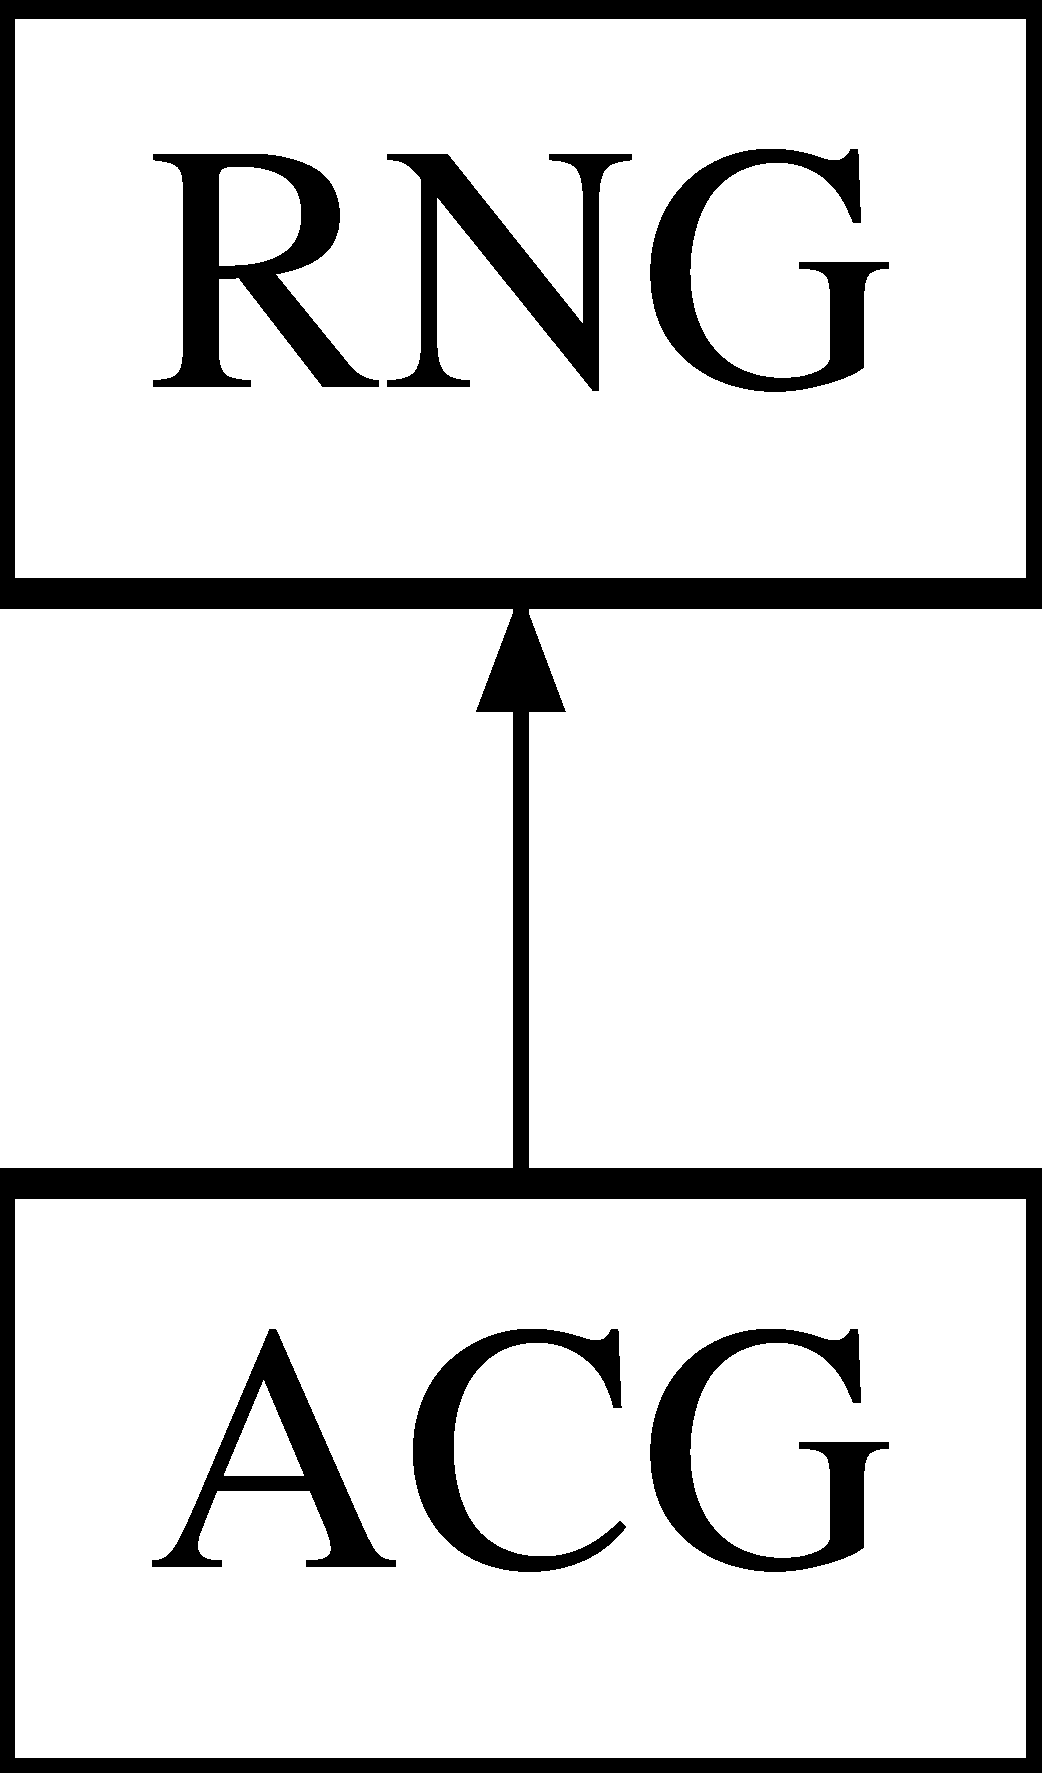
\includegraphics[height=2.000000cm]{classACG}
\end{center}
\end{figure}
\subsection*{Public Member Functions}
\begin{DoxyCompactItemize}
\item 
\mbox{\Hypertarget{classACG_ab574de6ba1590b838b3235fefb503041}\label{classACG_ab574de6ba1590b838b3235fefb503041}} 
{\bfseries A\+CG} (\+\_\+\+G\+\_\+uint32\+\_\+t seed=0, int size=55)
\item 
\mbox{\Hypertarget{classACG_ab2fa5f8178d29fe1f3d97529fa439df3}\label{classACG_ab2fa5f8178d29fe1f3d97529fa439df3}} 
virtual unsigned int {\bfseries as\+Long} ()
\item 
\mbox{\Hypertarget{classACG_a8cae86432d64c79199acb140019a0c6f}\label{classACG_a8cae86432d64c79199acb140019a0c6f}} 
virtual void {\bfseries reset} ()
\end{DoxyCompactItemize}


The documentation for this class was generated from the following files\+:\begin{DoxyCompactItemize}
\item 
/home/fallon/git/merlin-\/cmake/\+Merlin/A\+C\+G.\+h\item 
/home/fallon/git/merlin-\/cmake/\+Merlin/A\+C\+G.\+cpp\end{DoxyCompactItemize}

\hypertarget{classAMBufferManager}{}\section{A\+M\+Buffer\+Manager$<$ M, B, D $>$ Class Template Reference}
\label{classAMBufferManager}\index{A\+M\+Buffer\+Manager$<$ M, B, D $>$@{A\+M\+Buffer\+Manager$<$ M, B, D $>$}}
\subsection*{Public Member Functions}
\begin{DoxyCompactItemize}
\item 
\mbox{\Hypertarget{classAMBufferManager_a13820bc70783c397947c0f1bba2f58fe}\label{classAMBufferManager_a13820bc70783c397947c0f1bba2f58fe}} 
void {\bfseries Add\+Buffer} (B $\ast$buf)
\item 
\mbox{\Hypertarget{classAMBufferManager_a951f25ba53f19c8f9eba4f3030275d08}\label{classAMBufferManager_a951f25ba53f19c8f9eba4f3030275d08}} 
bool {\bfseries Remove\+Buffer} (B $\ast$buf)
\item 
\mbox{\Hypertarget{classAMBufferManager_ad0b5cb9c008ef288566afcbd3389060a}\label{classAMBufferManager_ad0b5cb9c008ef288566afcbd3389060a}} 
void {\bfseries Clear\+All\+Buffers} ()
\item 
\mbox{\Hypertarget{classAMBufferManager_a5ffab8073fc4b5d7255bd723ffe9fde8}\label{classAMBufferManager_a5ffab8073fc4b5d7255bd723ffe9fde8}} 
void {\bfseries Send\+To\+Buffers} (const M \&monitor, const D \&data)
\item 
\mbox{\Hypertarget{classAMBufferManager_a3f266c61b388badd6c4d37ffd16e4d09}\label{classAMBufferManager_a3f266c61b388badd6c4d37ffd16e4d09}} 
bool {\bfseries empty} () const
\end{DoxyCompactItemize}
\subsection*{Static Public Member Functions}
\begin{DoxyCompactItemize}
\item 
\mbox{\Hypertarget{classAMBufferManager_a031dca55ec86390f314ce595871519c8}\label{classAMBufferManager_a031dca55ec86390f314ce595871519c8}} 
static void {\bfseries Set\+Default\+Buffer} (B $\ast$buf)
\end{DoxyCompactItemize}


The documentation for this class was generated from the following file\+:\begin{DoxyCompactItemize}
\item 
/home/fallon/git/merlin-\/cmake/\+Merlin/A\+M\+Buffer\+Manager.\+h\end{DoxyCompactItemize}

\hypertarget{structInterpolatedAperture_1_1ap}{}\section{Interpolated\+Aperture\+:\+:ap Struct Reference}
\label{structInterpolatedAperture_1_1ap}\index{Interpolated\+Aperture\+::ap@{Interpolated\+Aperture\+::ap}}
\subsection*{Public Attributes}
\begin{DoxyCompactItemize}
\item 
\mbox{\Hypertarget{structInterpolatedAperture_1_1ap_a0759a9aa95c7a0e25336b26eb15ff4ca}\label{structInterpolatedAperture_1_1ap_a0759a9aa95c7a0e25336b26eb15ff4ca}} 
double {\bfseries s}
\item 
\mbox{\Hypertarget{structInterpolatedAperture_1_1ap_a3d62c47aeda602381be5cef93f7e3025}\label{structInterpolatedAperture_1_1ap_a3d62c47aeda602381be5cef93f7e3025}} 
double {\bfseries ap1}
\item 
\mbox{\Hypertarget{structInterpolatedAperture_1_1ap_a1b71fc032ac1b791ef2f77c6fb05caf2}\label{structInterpolatedAperture_1_1ap_a1b71fc032ac1b791ef2f77c6fb05caf2}} 
double {\bfseries ap2}
\item 
\mbox{\Hypertarget{structInterpolatedAperture_1_1ap_ae23652da42c61ac5686612ff5ed05d34}\label{structInterpolatedAperture_1_1ap_ae23652da42c61ac5686612ff5ed05d34}} 
double {\bfseries ap3}
\item 
\mbox{\Hypertarget{structInterpolatedAperture_1_1ap_afa60ba260c28653c614de5684146ebb9}\label{structInterpolatedAperture_1_1ap_afa60ba260c28653c614de5684146ebb9}} 
double {\bfseries ap4}
\item 
\mbox{\Hypertarget{structInterpolatedAperture_1_1ap_ac986e548358501ff50a66e4dc5c1102e}\label{structInterpolatedAperture_1_1ap_ac986e548358501ff50a66e4dc5c1102e}} 
\hyperlink{classInterpolatedAperture_a39433c0172ff3f57ea3daefaff6fcc74}{Aperture\+Class\+\_\+t} {\bfseries Ap\+Type}
\end{DoxyCompactItemize}


The documentation for this struct was generated from the following file\+:\begin{DoxyCompactItemize}
\item 
/home/fallon/git/merlin-\/cmake/\+Merlin/Interpolated\+Apertures.\+h\end{DoxyCompactItemize}

\hypertarget{structApertureConfiguration_1_1ap}{}\section{Aperture\+Configuration\+:\+:ap Struct Reference}
\label{structApertureConfiguration_1_1ap}\index{Aperture\+Configuration\+::ap@{Aperture\+Configuration\+::ap}}


{\ttfamily \#include $<$Aperture\+Configuration.\+h$>$}

\subsection*{Public Attributes}
\begin{DoxyCompactItemize}
\item 
\mbox{\Hypertarget{structApertureConfiguration_1_1ap_a662b14825383706cfb1548a9af083659}\label{structApertureConfiguration_1_1ap_a662b14825383706cfb1548a9af083659}} 
double {\bfseries s}
\item 
\mbox{\Hypertarget{structApertureConfiguration_1_1ap_adac536334e262f6d77863d37035c580f}\label{structApertureConfiguration_1_1ap_adac536334e262f6d77863d37035c580f}} 
double {\bfseries ap1}
\item 
\mbox{\Hypertarget{structApertureConfiguration_1_1ap_a0307ca82001fedad44736c53cd620291}\label{structApertureConfiguration_1_1ap_a0307ca82001fedad44736c53cd620291}} 
double {\bfseries ap2}
\item 
\mbox{\Hypertarget{structApertureConfiguration_1_1ap_a77f2d801233879025e5502434364da89}\label{structApertureConfiguration_1_1ap_a77f2d801233879025e5502434364da89}} 
double {\bfseries ap3}
\item 
\mbox{\Hypertarget{structApertureConfiguration_1_1ap_ab9d4875c612d163f4583ad2e27c68165}\label{structApertureConfiguration_1_1ap_ab9d4875c612d163f4583ad2e27c68165}} 
double {\bfseries ap4}
\item 
\mbox{\Hypertarget{structApertureConfiguration_1_1ap_a86afc7bed14928c846b70d358efc740c}\label{structApertureConfiguration_1_1ap_a86afc7bed14928c846b70d358efc740c}} 
\hyperlink{classApertureConfiguration_a84c9eaffaf4394f1538d2ec57a85c706}{Aperture\+Class\+\_\+t} {\bfseries Ap\+Type}
\end{DoxyCompactItemize}


\subsection{Detailed Description}
See the M\+AD users guide for how these apertures are defined. (current as of V5.\+02.\+07) \href{http://madx.web.cern.ch/madx/releases/last-dev/madxuguide.pdf}{\tt http\+://madx.\+web.\+cern.\+ch/madx/releases/last-\/dev/madxuguide.\+pdf} \char`\"{}\+Physical Aperture\+: Aperture definition\char`\"{}

Interpolated in this case is where one type joins another -\/ internal usage, not a M\+A\+D-\/X type. 

The documentation for this struct was generated from the following file\+:\begin{DoxyCompactItemize}
\item 
/home/fallon/git/merlin-\/cmake/\+Merlin/Aperture\+Configuration.\+h\end{DoxyCompactItemize}

\hypertarget{classAperture}{}\section{Aperture Class Reference}
\label{classAperture}\index{Aperture@{Aperture}}


{\ttfamily \#include $<$Aperture.\+h$>$}

Inheritance diagram for Aperture\+:\begin{figure}[H]
\begin{center}
\leavevmode
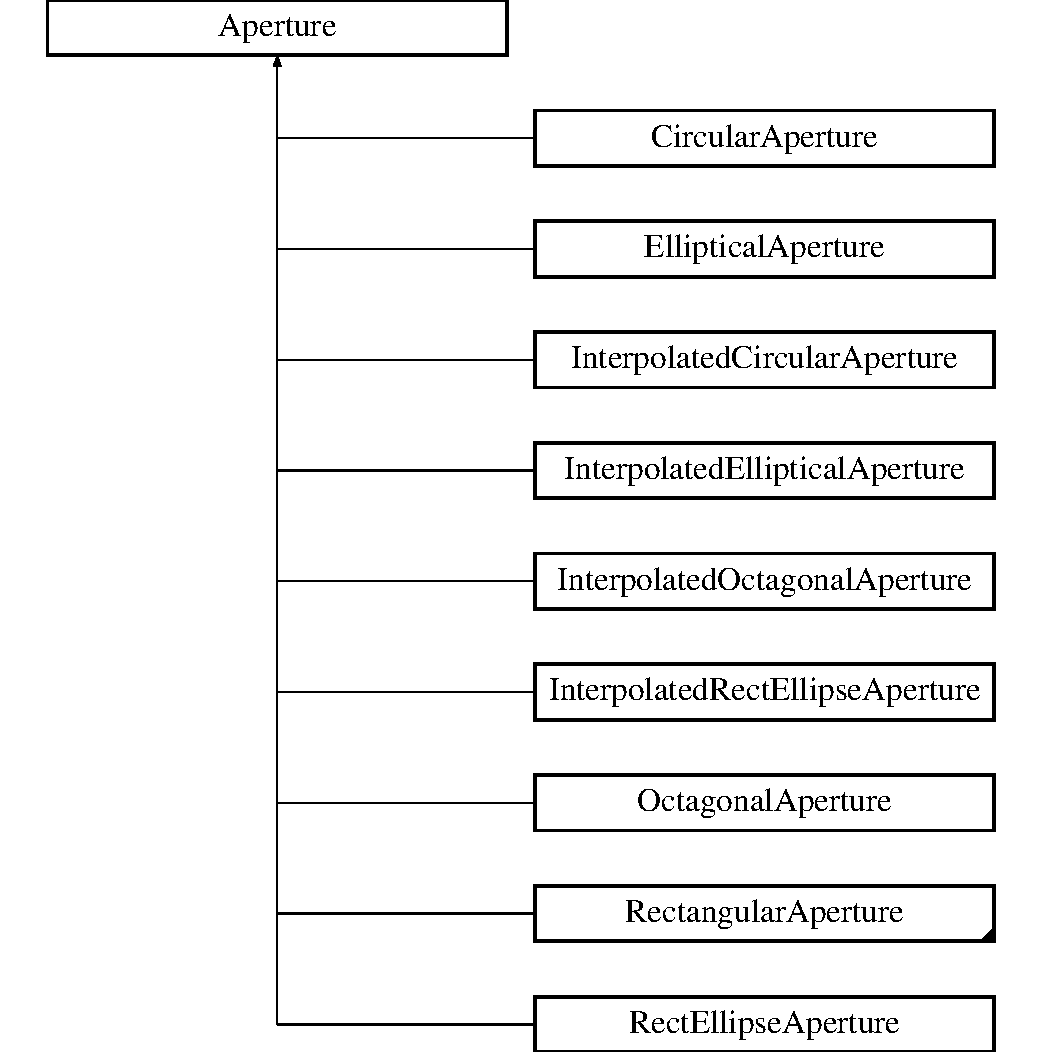
\includegraphics[height=10.000000cm]{classAperture}
\end{center}
\end{figure}
\subsection*{Public Member Functions}
\begin{DoxyCompactItemize}
\item 
\hyperlink{classAperture_ad20a215bea35fe695d98c1d4e000112f}{Aperture} (\hyperlink{classMaterial}{Material} $\ast$m=nullptr)
\item 
virtual \hyperlink{classAperture_ad2ec00bf784a25710ce4049f339513d6}{$\sim$\+Aperture} ()
\item 
virtual bool \hyperlink{classAperture_a77854d058bf8a00cfeb7a6d766dc0028}{Point\+Inside} (double x, double y, double z) const =0
\item 
bool \hyperlink{classAperture_a3fe1acdd1ca1792a7df9305b2ff6e454}{Point\+Inside} (const \hyperlink{classTVec3D}{Point3D} \&p) const
\item 
virtual double \hyperlink{classAperture_ad0ea7907d393ec1e6a8303343fe9dd29}{Get\+Radius\+At} (double phi, double z) const =0
\item 
virtual std\+::string \hyperlink{classAperture_ad7af612271a0586feea83c38549dfb75}{Get\+Aperture\+Type} () const =0
\item 
\hyperlink{classMaterial}{Material} $\ast$ \hyperlink{classAperture_ae75acab11fe8687836cd71afe80e9dd2}{Get\+Material} () const
\item 
void \hyperlink{classAperture_aa35484166441c2be0e2e159c6d6f4a11}{Set\+Material} (\hyperlink{classMaterial}{Material} $\ast$m)
\item 
virtual void \hyperlink{classAperture_aff2f276b93bb2cb94e559e1c4901e38e}{printout} (std\+::ostream \&out) const
\end{DoxyCompactItemize}
\subsection*{Protected Attributes}
\begin{DoxyCompactItemize}
\item 
\hyperlink{classMaterial}{Material} $\ast$ \hyperlink{classAperture_ae92ba16dcfebf1949db67b8fc0ae3c7b}{Aperture\+Material}
\end{DoxyCompactItemize}


\subsection{Detailed Description}
Represents the cross section of the vacuum pipe or other collimating aperture. 

\subsection{Constructor \& Destructor Documentation}
\mbox{\Hypertarget{classAperture_ad20a215bea35fe695d98c1d4e000112f}\label{classAperture_ad20a215bea35fe695d98c1d4e000112f}} 
\index{Aperture@{Aperture}!Aperture@{Aperture}}
\index{Aperture@{Aperture}!Aperture@{Aperture}}
\subsubsection{\texorpdfstring{Aperture()}{Aperture()}}
{\footnotesize\ttfamily Aperture\+::\+Aperture (\begin{DoxyParamCaption}\item[{\hyperlink{classMaterial}{Material} $\ast$}]{m = {\ttfamily nullptr} }\end{DoxyParamCaption})\hspace{0.3cm}{\ttfamily [inline]}}

Constructor 
\begin{DoxyParams}[1]{Parameters}
\mbox{\tt in}  & {\em m} & The material to attach to this aperture. \\
\hline
\end{DoxyParams}
\mbox{\Hypertarget{classAperture_ad2ec00bf784a25710ce4049f339513d6}\label{classAperture_ad2ec00bf784a25710ce4049f339513d6}} 
\index{Aperture@{Aperture}!````~Aperture@{$\sim$\+Aperture}}
\index{````~Aperture@{$\sim$\+Aperture}!Aperture@{Aperture}}
\subsubsection{\texorpdfstring{$\sim$\+Aperture()}{~Aperture()}}
{\footnotesize\ttfamily Aperture\+::$\sim$\+Aperture (\begin{DoxyParamCaption}{ }\end{DoxyParamCaption})\hspace{0.3cm}{\ttfamily [virtual]}}

Destructor 

\subsection{Member Function Documentation}
\mbox{\Hypertarget{classAperture_ad7af612271a0586feea83c38549dfb75}\label{classAperture_ad7af612271a0586feea83c38549dfb75}} 
\index{Aperture@{Aperture}!Get\+Aperture\+Type@{Get\+Aperture\+Type}}
\index{Get\+Aperture\+Type@{Get\+Aperture\+Type}!Aperture@{Aperture}}
\subsubsection{\texorpdfstring{Get\+Aperture\+Type()}{GetApertureType()}}
{\footnotesize\ttfamily virtual std\+::string Aperture\+::\+Get\+Aperture\+Type (\begin{DoxyParamCaption}{ }\end{DoxyParamCaption}) const\hspace{0.3cm}{\ttfamily [pure virtual]}}

Returns the type of the aperture. \begin{DoxyReturn}{Returns}
A string containing the type of the aperture. 
\end{DoxyReturn}


Implemented in \hyperlink{classOctagonalAperture_ada756a63c21912b26d79a5743bbd051f}{Octagonal\+Aperture}, \hyperlink{classEllipticalAperture_a8c56e3ab5e8483dd42ed6e35855409df}{Elliptical\+Aperture}, \hyperlink{classInterpolatedOctagonalAperture_a9e16536001e2732bcaf15d55134e05bf}{Interpolated\+Octagonal\+Aperture}, \hyperlink{classInterpolatedEllipticalAperture_a02a87b57b089796ccf55c9bbe16a11ec}{Interpolated\+Elliptical\+Aperture}, \hyperlink{classInterpolatedCircularAperture_ad6c2112ec4e0bd1b21b679e3fab08704}{Interpolated\+Circular\+Aperture}, \hyperlink{classCircularAperture_a18f05ba1dde35881014ba3aa2ed693bc}{Circular\+Aperture}, \hyperlink{classInterpolatedRectEllipseAperture_a310886ba54e5ea6a4e95d8946c9a7440}{Interpolated\+Rect\+Ellipse\+Aperture}, \hyperlink{classRectangularAperture_ac7d8e273423b18e1898286a51e3f22c7}{Rectangular\+Aperture}, and \hyperlink{classRectEllipseAperture_a983dec943872b82aa91f74cd10558207}{Rect\+Ellipse\+Aperture}.

\mbox{\Hypertarget{classAperture_ae75acab11fe8687836cd71afe80e9dd2}\label{classAperture_ae75acab11fe8687836cd71afe80e9dd2}} 
\index{Aperture@{Aperture}!Get\+Material@{Get\+Material}}
\index{Get\+Material@{Get\+Material}!Aperture@{Aperture}}
\subsubsection{\texorpdfstring{Get\+Material()}{GetMaterial()}}
{\footnotesize\ttfamily \hyperlink{classMaterial}{Material} $\ast$ Aperture\+::\+Get\+Material (\begin{DoxyParamCaption}{ }\end{DoxyParamCaption}) const}

Gets the material associated with this aperture. \begin{DoxyReturn}{Returns}
A pointer to a \hyperlink{classMaterial}{Material} class attached to this aperture. 
\end{DoxyReturn}
\mbox{\Hypertarget{classAperture_ad0ea7907d393ec1e6a8303343fe9dd29}\label{classAperture_ad0ea7907d393ec1e6a8303343fe9dd29}} 
\index{Aperture@{Aperture}!Get\+Radius\+At@{Get\+Radius\+At}}
\index{Get\+Radius\+At@{Get\+Radius\+At}!Aperture@{Aperture}}
\subsubsection{\texorpdfstring{Get\+Radius\+At()}{GetRadiusAt()}}
{\footnotesize\ttfamily virtual double Aperture\+::\+Get\+Radius\+At (\begin{DoxyParamCaption}\item[{double}]{phi,  }\item[{double}]{z }\end{DoxyParamCaption}) const\hspace{0.3cm}{\ttfamily [pure virtual]}}

Returns the radius to the aperture at location z and angle phi. 
\begin{DoxyParams}[1]{Parameters}
\mbox{\tt in}  & {\em phi} & The angle. \\
\hline
\mbox{\tt in}  & {\em z} & The z position of the particle. \\
\hline
\end{DoxyParams}
\begin{DoxyReturn}{Returns}
A double containing the aperture radius. 
\end{DoxyReturn}


Implemented in \hyperlink{classOctagonalAperture_ab79ca14c1d75522637bea3ffbbb0d8a4}{Octagonal\+Aperture}, \hyperlink{classEllipticalAperture_aec41ce72d82e004b8de123e37d3b11e9}{Elliptical\+Aperture}, \hyperlink{classInterpolatedOctagonalAperture_a92937e111009433a274722eb316270e1}{Interpolated\+Octagonal\+Aperture}, \hyperlink{classInterpolatedEllipticalAperture_adcbc99d397eba723e88877d199c035d8}{Interpolated\+Elliptical\+Aperture}, \hyperlink{classInterpolatedCircularAperture_a4c614ba51b5da0e01808f719f6a7511f}{Interpolated\+Circular\+Aperture}, \hyperlink{classCircularAperture_ab2f83be4d78bb1495b2b0aebef78e189}{Circular\+Aperture}, \hyperlink{classInterpolatedRectEllipseAperture_aac0970213673334851109d69e0e6a423}{Interpolated\+Rect\+Ellipse\+Aperture}, \hyperlink{classRectangularAperture_a7ef1ddd66a755305b7bab2a2c3ac5d58}{Rectangular\+Aperture}, and \hyperlink{classRectEllipseAperture_a3e6ea0e15b7a9f026bc7ead70efe5e18}{Rect\+Ellipse\+Aperture}.

\mbox{\Hypertarget{classAperture_a77854d058bf8a00cfeb7a6d766dc0028}\label{classAperture_a77854d058bf8a00cfeb7a6d766dc0028}} 
\index{Aperture@{Aperture}!Point\+Inside@{Point\+Inside}}
\index{Point\+Inside@{Point\+Inside}!Aperture@{Aperture}}
\subsubsection{\texorpdfstring{Point\+Inside()}{PointInside()}\hspace{0.1cm}{\footnotesize\ttfamily [1/2]}}
{\footnotesize\ttfamily virtual bool Aperture\+::\+Point\+Inside (\begin{DoxyParamCaption}\item[{double}]{x,  }\item[{double}]{y,  }\item[{double}]{z }\end{DoxyParamCaption}) const\hspace{0.3cm}{\ttfamily [pure virtual]}}

Returns true if the point (x,y,z) is within the aperture. 
\begin{DoxyParams}[1]{Parameters}
\mbox{\tt in}  & {\em x} & The x coordinate of the particle \\
\hline
\mbox{\tt in}  & {\em y} & The y coordinate of the particle \\
\hline
\mbox{\tt in}  & {\em z} & The z coordinate of the particle \\
\hline
\end{DoxyParams}
\begin{DoxyReturn}{Returns}
A bool set to true if the specified point, is within the \hyperlink{classAperture}{Aperture}. false if it is not. 
\end{DoxyReturn}


Implemented in \hyperlink{classOctagonalAperture_a9c3e4ba8a96d3b97fc92fdeef975caf9}{Octagonal\+Aperture}, \hyperlink{classEllipticalAperture_ad2ac194f4f03d5e590a7640afa69ace9}{Elliptical\+Aperture}, \hyperlink{classInterpolatedOctagonalAperture_a7d2e6993a0d679e23038ca88245db59b}{Interpolated\+Octagonal\+Aperture}, \hyperlink{classInterpolatedEllipticalAperture_a2e0b148eea71b6651cdf78df66d69e62}{Interpolated\+Elliptical\+Aperture}, \hyperlink{classOneSidedUnalignedCollimatorAperture_afad818345b971dffa9ca6fa36a166e35}{One\+Sided\+Unaligned\+Collimator\+Aperture}, \hyperlink{classInterpolatedCircularAperture_aeb31875191b05bd63bd00fe11294a432}{Interpolated\+Circular\+Aperture}, \hyperlink{classCircularAperture_a1cc2c7d1ff491dbfb0c24790897d4519}{Circular\+Aperture}, \hyperlink{classUnalignedCollimatorAperture_af116c2ff1d60c4894a9b9ae4cfc2b19e}{Unaligned\+Collimator\+Aperture}, \hyperlink{classInterpolatedRectEllipseAperture_a53862c9efd9d7e090e08ff027b6b80cf}{Interpolated\+Rect\+Ellipse\+Aperture}, \hyperlink{classCollimatorAperture_a964f63287a0ab48900859d75dfa644dc}{Collimator\+Aperture}, \hyperlink{classRectangularAperture_a47e965df14eb63f2a3851ea0e9fe26db}{Rectangular\+Aperture}, and \hyperlink{classRectEllipseAperture_ac3cc7fae775b055d74ea185a77b08c7f}{Rect\+Ellipse\+Aperture}.

\mbox{\Hypertarget{classAperture_a3fe1acdd1ca1792a7df9305b2ff6e454}\label{classAperture_a3fe1acdd1ca1792a7df9305b2ff6e454}} 
\index{Aperture@{Aperture}!Point\+Inside@{Point\+Inside}}
\index{Point\+Inside@{Point\+Inside}!Aperture@{Aperture}}
\subsubsection{\texorpdfstring{Point\+Inside()}{PointInside()}\hspace{0.1cm}{\footnotesize\ttfamily [2/2]}}
{\footnotesize\ttfamily bool Aperture\+::\+Point\+Inside (\begin{DoxyParamCaption}\item[{const \hyperlink{classTVec3D}{Point3D} \&}]{p }\end{DoxyParamCaption}) const\hspace{0.3cm}{\ttfamily [inline]}}

Returns true if the point p is within the aperture. 
\begin{DoxyParams}[1]{Parameters}
\mbox{\tt in}  & {\em p} & 3D point reference to check \\
\hline
\end{DoxyParams}
\begin{DoxyReturn}{Returns}
A bool set to true if the specified point, is within the \hyperlink{classAperture}{Aperture}. false if it is not. 
\end{DoxyReturn}
\mbox{\Hypertarget{classAperture_aff2f276b93bb2cb94e559e1c4901e38e}\label{classAperture_aff2f276b93bb2cb94e559e1c4901e38e}} 
\index{Aperture@{Aperture}!printout@{printout}}
\index{printout@{printout}!Aperture@{Aperture}}
\subsubsection{\texorpdfstring{printout()}{printout()}}
{\footnotesize\ttfamily void Aperture\+::printout (\begin{DoxyParamCaption}\item[{std\+::ostream \&}]{out }\end{DoxyParamCaption}) const\hspace{0.3cm}{\ttfamily [virtual]}}

Prints out the \hyperlink{classAperture}{Aperture} parameters to a specified stream. 
\begin{DoxyParams}[1]{Parameters}
\mbox{\tt out}  & {\em out} & The output stream to use. \\
\hline
\end{DoxyParams}


Reimplemented in \hyperlink{classOctagonalAperture_ad8329324a912bc76c97fd3f8bbefa5ac}{Octagonal\+Aperture}, \hyperlink{classEllipticalAperture_af45343465b84072027de770839bbd73d}{Elliptical\+Aperture}, \hyperlink{classInterpolatedOctagonalAperture_ad1e9dcb72289db534c78e297fa4c8197}{Interpolated\+Octagonal\+Aperture}, \hyperlink{classInterpolatedEllipticalAperture_aee15c62d0ff01c37120481cc821f9d87}{Interpolated\+Elliptical\+Aperture}, \hyperlink{classInterpolatedCircularAperture_af32b8d603ed9dd511c3b00a045400795}{Interpolated\+Circular\+Aperture}, \hyperlink{classCircularAperture_af7380933fd3494dd0d1868b655a78b08}{Circular\+Aperture}, \hyperlink{classInterpolatedRectEllipseAperture_abd88d2108988e8653517e3291dd92ff2}{Interpolated\+Rect\+Ellipse\+Aperture}, \hyperlink{classRectangularAperture_ab3a9514337b3fd3f2368f03ab6410533}{Rectangular\+Aperture}, and \hyperlink{classRectEllipseAperture_a13285bdfb9c849fe94cd261ae1bfffe4}{Rect\+Ellipse\+Aperture}.

\mbox{\Hypertarget{classAperture_aa35484166441c2be0e2e159c6d6f4a11}\label{classAperture_aa35484166441c2be0e2e159c6d6f4a11}} 
\index{Aperture@{Aperture}!Set\+Material@{Set\+Material}}
\index{Set\+Material@{Set\+Material}!Aperture@{Aperture}}
\subsubsection{\texorpdfstring{Set\+Material()}{SetMaterial()}}
{\footnotesize\ttfamily void Aperture\+::\+Set\+Material (\begin{DoxyParamCaption}\item[{\hyperlink{classMaterial}{Material} $\ast$}]{m }\end{DoxyParamCaption})}

Sets the material associated with this aperture. 
\begin{DoxyParams}[1]{Parameters}
\mbox{\tt in}  & {\em m} & The material to attach to this aperture. \\
\hline
\end{DoxyParams}


\subsection{Member Data Documentation}
\mbox{\Hypertarget{classAperture_ae92ba16dcfebf1949db67b8fc0ae3c7b}\label{classAperture_ae92ba16dcfebf1949db67b8fc0ae3c7b}} 
\index{Aperture@{Aperture}!Aperture\+Material@{Aperture\+Material}}
\index{Aperture\+Material@{Aperture\+Material}!Aperture@{Aperture}}
\subsubsection{\texorpdfstring{Aperture\+Material}{ApertureMaterial}}
{\footnotesize\ttfamily \hyperlink{classMaterial}{Material}$\ast$ Aperture\+::\+Aperture\+Material\hspace{0.3cm}{\ttfamily [protected]}}

The \hyperlink{classMaterial}{Material} of this aperture. 

The documentation for this class was generated from the following files\+:\begin{DoxyCompactItemize}
\item 
/home/fallon/git/merlin-\/cmake/\+Merlin/Aperture.\+h\item 
/home/fallon/git/merlin-\/cmake/\+Merlin/Aperture.\+cpp\end{DoxyCompactItemize}

\hypertarget{classApertureConfiguration}{}\section{Aperture\+Configuration Class Reference}
\label{classApertureConfiguration}\index{Aperture\+Configuration@{Aperture\+Configuration}}
\subsection*{Classes}
\begin{DoxyCompactItemize}
\item 
struct \hyperlink{structApertureConfiguration_1_1ap}{ap}
\end{DoxyCompactItemize}
\subsection*{Public Types}
\begin{DoxyCompactItemize}
\item 
typedef size\+\_\+t \hyperlink{classApertureConfiguration_a84c9eaffaf4394f1538d2ec57a85c706}{Aperture\+Class\+\_\+t}
\end{DoxyCompactItemize}
\subsection*{Public Member Functions}
\begin{DoxyCompactItemize}
\item 
\hyperlink{classApertureConfiguration_ac9b95b8adbd178d7345cd147000d7038}{Aperture\+Configuration} ()
\item 
\hyperlink{classApertureConfiguration_affd6ff3a6500fb8b7aecc5d8cc7d5ab5}{Aperture\+Configuration} (std\+::string Input\+File\+Name)
\item 
void \hyperlink{classApertureConfiguration_a23e6989301d2c88027decc4c6cf63049}{Load\+Aperture\+Configuration} (std\+::string Input\+File\+Name)
\item 
void \hyperlink{classApertureConfiguration_ac57cc418854b69b0893c8a0c36386ace}{Output\+Aperture\+List} (std\+::ostream \&os)
\item 
void \hyperlink{classApertureConfiguration_af954151209360897a506d914f922f03f}{Configure\+Element\+Apertures} (\hyperlink{classAcceleratorModel}{Accelerator\+Model} $\ast$)
\item 
void \hyperlink{classApertureConfiguration_a18b3907d726e2ef8731d6fe9a8a50ea4}{Delete\+All\+Apertures} (\hyperlink{classAcceleratorModel}{Accelerator\+Model} $\ast$Model)
\item 
void \hyperlink{classApertureConfiguration_a2def09944077a1c8048ea201256234a5}{Set\+Log\+File} (ostream \&os)
\item 
void \hyperlink{classApertureConfiguration_acbb9431d139a07249cf0487f8fd4753b}{Enable\+Logging} (bool flag)
\item 
void \hyperlink{classApertureConfiguration_a71fec510b3f362a5307ffde2fb876ab7}{Set\+Default\+Aperture} (\hyperlink{classAperture}{Aperture} $\ast$\hyperlink{structApertureConfiguration_1_1ap}{ap})
\item 
void \hyperlink{classApertureConfiguration_a24391451e6a25bc59ea448bdf06bb1b4}{Enable\+Default\+Aperture} (bool flag)
\end{DoxyCompactItemize}
\subsection*{Public Attributes}
\begin{DoxyCompactItemize}
\item 
std\+::ostream $\ast$ \hyperlink{classApertureConfiguration_a14da0e53d6b7306ad417dfa51f4d7470}{log}
\item 
bool \hyperlink{classApertureConfiguration_ad4005122e0a206a8376407ed8c54c0f6}{log\+Flag}
\item 
\hyperlink{structApertureConfiguration_1_1ap}{ap} \hyperlink{classApertureConfiguration_a20692047dd6ec339da5bf9e80f9f9f3c}{Aperture\+Entry}
\item 
std\+::vector$<$ \hyperlink{structApertureConfiguration_1_1ap}{ap} $>$ \hyperlink{classApertureConfiguration_a4b70556fb8ac55e8fb5d3d3e0b75b039}{Aperture\+List}
\item 
\hyperlink{classAperture}{Aperture} $\ast$ \hyperlink{classApertureConfiguration_a3b08ff20e5bbbb3d28d73048e1933f9f}{Default\+Aperture}
\item 
\mbox{\Hypertarget{classApertureConfiguration_ac7d2024a3d3b062f50733c2106fba998}\label{classApertureConfiguration_ac7d2024a3d3b062f50733c2106fba998}} 
bool {\bfseries Default\+Aperture\+Flag}
\end{DoxyCompactItemize}


\subsection{Member Typedef Documentation}
\mbox{\Hypertarget{classApertureConfiguration_a84c9eaffaf4394f1538d2ec57a85c706}\label{classApertureConfiguration_a84c9eaffaf4394f1538d2ec57a85c706}} 
\index{Aperture\+Configuration@{Aperture\+Configuration}!Aperture\+Class\+\_\+t@{Aperture\+Class\+\_\+t}}
\index{Aperture\+Class\+\_\+t@{Aperture\+Class\+\_\+t}!Aperture\+Configuration@{Aperture\+Configuration}}
\subsubsection{\texorpdfstring{Aperture\+Class\+\_\+t}{ApertureClass\_t}}
{\footnotesize\ttfamily typedef size\+\_\+t \hyperlink{classApertureConfiguration_a84c9eaffaf4394f1538d2ec57a85c706}{Aperture\+Configuration\+::\+Aperture\+Class\+\_\+t}}

Typedef for access to the enum 

\subsection{Constructor \& Destructor Documentation}
\mbox{\Hypertarget{classApertureConfiguration_ac9b95b8adbd178d7345cd147000d7038}\label{classApertureConfiguration_ac9b95b8adbd178d7345cd147000d7038}} 
\index{Aperture\+Configuration@{Aperture\+Configuration}!Aperture\+Configuration@{Aperture\+Configuration}}
\index{Aperture\+Configuration@{Aperture\+Configuration}!Aperture\+Configuration@{Aperture\+Configuration}}
\subsubsection{\texorpdfstring{Aperture\+Configuration()}{ApertureConfiguration()}\hspace{0.1cm}{\footnotesize\ttfamily [1/2]}}
{\footnotesize\ttfamily Aperture\+Configuration\+::\+Aperture\+Configuration (\begin{DoxyParamCaption}{ }\end{DoxyParamCaption})}

Constructor \mbox{\Hypertarget{classApertureConfiguration_affd6ff3a6500fb8b7aecc5d8cc7d5ab5}\label{classApertureConfiguration_affd6ff3a6500fb8b7aecc5d8cc7d5ab5}} 
\index{Aperture\+Configuration@{Aperture\+Configuration}!Aperture\+Configuration@{Aperture\+Configuration}}
\index{Aperture\+Configuration@{Aperture\+Configuration}!Aperture\+Configuration@{Aperture\+Configuration}}
\subsubsection{\texorpdfstring{Aperture\+Configuration()}{ApertureConfiguration()}\hspace{0.1cm}{\footnotesize\ttfamily [2/2]}}
{\footnotesize\ttfamily Aperture\+Configuration\+::\+Aperture\+Configuration (\begin{DoxyParamCaption}\item[{std\+::string}]{Input\+File\+Name }\end{DoxyParamCaption})}

Constructor with an input file to load 
\begin{DoxyParams}[1]{Parameters}
\mbox{\tt in}  & {\em Input\+File\+Name} & The name of the aperture file to load \\
\hline
\end{DoxyParams}


\subsection{Member Function Documentation}
\mbox{\Hypertarget{classApertureConfiguration_af954151209360897a506d914f922f03f}\label{classApertureConfiguration_af954151209360897a506d914f922f03f}} 
\index{Aperture\+Configuration@{Aperture\+Configuration}!Configure\+Element\+Apertures@{Configure\+Element\+Apertures}}
\index{Configure\+Element\+Apertures@{Configure\+Element\+Apertures}!Aperture\+Configuration@{Aperture\+Configuration}}
\subsubsection{\texorpdfstring{Configure\+Element\+Apertures()}{ConfigureElementApertures()}}
{\footnotesize\ttfamily void Aperture\+Configuration\+::\+Configure\+Element\+Apertures (\begin{DoxyParamCaption}\item[{\hyperlink{classAcceleratorModel}{Accelerator\+Model} $\ast$}]{Model }\end{DoxyParamCaption})}

Configures the beam pipe for a given accelerator model 
\begin{DoxyParams}[1]{Parameters}
\mbox{\tt in}  & {\em Model} & A pointer to the \hyperlink{classAcceleratorModel}{Accelerator\+Model} class to add the apertures to \\
\hline
\end{DoxyParams}
Elements -\/ The container with all \hyperlink{classAcceleratorComponent}{Accelerator\+Component} entries comp -\/ Iterator to all \hyperlink{classAcceleratorComponent}{Accelerator\+Component} entries

Aperture\+List -\/ The container with all \hyperlink{classAperture}{Aperture} entries itr -\/ Iterator to all \hyperlink{classAperture}{Aperture} entries.

This\+Element\+Aperture -\/ The container for the current element \hyperlink{classAperture}{Aperture}.

Give magnets and other fixed elements a set aperture. Give drifts interpolated apertures.

3 possible cases 1\+: First entry in the element (or accelerator) 2\+: Entries within an element 3\+: Final entry within an element (or accelerator)

Now move on to assigning the correct type of aperture.

Check if all values are constant\mbox{\Hypertarget{classApertureConfiguration_a18b3907d726e2ef8731d6fe9a8a50ea4}\label{classApertureConfiguration_a18b3907d726e2ef8731d6fe9a8a50ea4}} 
\index{Aperture\+Configuration@{Aperture\+Configuration}!Delete\+All\+Apertures@{Delete\+All\+Apertures}}
\index{Delete\+All\+Apertures@{Delete\+All\+Apertures}!Aperture\+Configuration@{Aperture\+Configuration}}
\subsubsection{\texorpdfstring{Delete\+All\+Apertures()}{DeleteAllApertures()}}
{\footnotesize\ttfamily void Aperture\+Configuration\+::\+Delete\+All\+Apertures (\begin{DoxyParamCaption}\item[{\hyperlink{classAcceleratorModel}{Accelerator\+Model} $\ast$}]{Model }\end{DoxyParamCaption})}

Deletes all apertures currently attached to the given accelerator model 
\begin{DoxyParams}[1]{Parameters}
\mbox{\tt in}  & {\em Model} & A pointer to the \hyperlink{classAcceleratorModel}{Accelerator\+Model} class to add the apertures to \\
\hline
\end{DoxyParams}
\mbox{\Hypertarget{classApertureConfiguration_a24391451e6a25bc59ea448bdf06bb1b4}\label{classApertureConfiguration_a24391451e6a25bc59ea448bdf06bb1b4}} 
\index{Aperture\+Configuration@{Aperture\+Configuration}!Enable\+Default\+Aperture@{Enable\+Default\+Aperture}}
\index{Enable\+Default\+Aperture@{Enable\+Default\+Aperture}!Aperture\+Configuration@{Aperture\+Configuration}}
\subsubsection{\texorpdfstring{Enable\+Default\+Aperture()}{EnableDefaultAperture()}}
{\footnotesize\ttfamily void Aperture\+Configuration\+::\+Enable\+Default\+Aperture (\begin{DoxyParamCaption}\item[{bool}]{flag }\end{DoxyParamCaption})}

Enable/disable use of the default aperture where it is not possible to clearly select an aperture type (e.\+g. O\+C\+T\+A\+G\+ON -\/$>$ R\+E\+C\+T\+E\+L\+L\+I\+P\+SE joins) 
\begin{DoxyParams}[1]{Parameters}
\mbox{\tt in}  & {\em flag} & A bool to enable or disable the usage of the default aperture \\
\hline
\end{DoxyParams}
\mbox{\Hypertarget{classApertureConfiguration_acbb9431d139a07249cf0487f8fd4753b}\label{classApertureConfiguration_acbb9431d139a07249cf0487f8fd4753b}} 
\index{Aperture\+Configuration@{Aperture\+Configuration}!Enable\+Logging@{Enable\+Logging}}
\index{Enable\+Logging@{Enable\+Logging}!Aperture\+Configuration@{Aperture\+Configuration}}
\subsubsection{\texorpdfstring{Enable\+Logging()}{EnableLogging()}}
{\footnotesize\ttfamily void Aperture\+Configuration\+::\+Enable\+Logging (\begin{DoxyParamCaption}\item[{bool}]{flag }\end{DoxyParamCaption})}

Enable/disable logging 
\begin{DoxyParams}[1]{Parameters}
\mbox{\tt in}  & {\em flag} & The requested logging state \\
\hline
\end{DoxyParams}
\mbox{\Hypertarget{classApertureConfiguration_a23e6989301d2c88027decc4c6cf63049}\label{classApertureConfiguration_a23e6989301d2c88027decc4c6cf63049}} 
\index{Aperture\+Configuration@{Aperture\+Configuration}!Load\+Aperture\+Configuration@{Load\+Aperture\+Configuration}}
\index{Load\+Aperture\+Configuration@{Load\+Aperture\+Configuration}!Aperture\+Configuration@{Aperture\+Configuration}}
\subsubsection{\texorpdfstring{Load\+Aperture\+Configuration()}{LoadApertureConfiguration()}}
{\footnotesize\ttfamily void Aperture\+Configuration\+::\+Load\+Aperture\+Configuration (\begin{DoxyParamCaption}\item[{std\+::string}]{Input\+File\+Name }\end{DoxyParamCaption})}

Load the \hyperlink{classAperture}{Aperture} settings from an input file. 
\begin{DoxyParams}[1]{Parameters}
\mbox{\tt in}  & {\em Input\+File\+Name} & The name of the aperture file to load \\
\hline
\end{DoxyParams}
\mbox{\Hypertarget{classApertureConfiguration_ac57cc418854b69b0893c8a0c36386ace}\label{classApertureConfiguration_ac57cc418854b69b0893c8a0c36386ace}} 
\index{Aperture\+Configuration@{Aperture\+Configuration}!Output\+Aperture\+List@{Output\+Aperture\+List}}
\index{Output\+Aperture\+List@{Output\+Aperture\+List}!Aperture\+Configuration@{Aperture\+Configuration}}
\subsubsection{\texorpdfstring{Output\+Aperture\+List()}{OutputApertureList()}}
{\footnotesize\ttfamily void Aperture\+Configuration\+::\+Output\+Aperture\+List (\begin{DoxyParamCaption}\item[{std\+::ostream \&}]{os }\end{DoxyParamCaption})}

Dumps the input file back out 
\begin{DoxyParams}[1]{Parameters}
\mbox{\tt in}  & {\em os} & The name of the stream to output to \\
\hline
\end{DoxyParams}
\mbox{\Hypertarget{classApertureConfiguration_a71fec510b3f362a5307ffde2fb876ab7}\label{classApertureConfiguration_a71fec510b3f362a5307ffde2fb876ab7}} 
\index{Aperture\+Configuration@{Aperture\+Configuration}!Set\+Default\+Aperture@{Set\+Default\+Aperture}}
\index{Set\+Default\+Aperture@{Set\+Default\+Aperture}!Aperture\+Configuration@{Aperture\+Configuration}}
\subsubsection{\texorpdfstring{Set\+Default\+Aperture()}{SetDefaultAperture()}}
{\footnotesize\ttfamily void Aperture\+Configuration\+::\+Set\+Default\+Aperture (\begin{DoxyParamCaption}\item[{\hyperlink{classAperture}{Aperture} $\ast$}]{ap }\end{DoxyParamCaption})}

Set a default class of aperture to use in ambiguous cases 
\begin{DoxyParams}[1]{Parameters}
\mbox{\tt in}  & {\em flag} & The requested logging state \\
\hline
\end{DoxyParams}
\mbox{\Hypertarget{classApertureConfiguration_a2def09944077a1c8048ea201256234a5}\label{classApertureConfiguration_a2def09944077a1c8048ea201256234a5}} 
\index{Aperture\+Configuration@{Aperture\+Configuration}!Set\+Log\+File@{Set\+Log\+File}}
\index{Set\+Log\+File@{Set\+Log\+File}!Aperture\+Configuration@{Aperture\+Configuration}}
\subsubsection{\texorpdfstring{Set\+Log\+File()}{SetLogFile()}}
{\footnotesize\ttfamily void Aperture\+Configuration\+::\+Set\+Log\+File (\begin{DoxyParamCaption}\item[{ostream \&}]{os }\end{DoxyParamCaption})}

Set the stream for the collimator settings log. 
\begin{DoxyParams}[1]{Parameters}
\mbox{\tt in}  & {\em os} & The stream to log the generated aperture to \\
\hline
\end{DoxyParams}


\subsection{Member Data Documentation}
\mbox{\Hypertarget{classApertureConfiguration_a20692047dd6ec339da5bf9e80f9f9f3c}\label{classApertureConfiguration_a20692047dd6ec339da5bf9e80f9f9f3c}} 
\index{Aperture\+Configuration@{Aperture\+Configuration}!Aperture\+Entry@{Aperture\+Entry}}
\index{Aperture\+Entry@{Aperture\+Entry}!Aperture\+Configuration@{Aperture\+Configuration}}
\subsubsection{\texorpdfstring{Aperture\+Entry}{ApertureEntry}}
{\footnotesize\ttfamily \hyperlink{structApertureConfiguration_1_1ap}{ap} Aperture\+Configuration\+::\+Aperture\+Entry}

One aperture entry \mbox{\Hypertarget{classApertureConfiguration_a4b70556fb8ac55e8fb5d3d3e0b75b039}\label{classApertureConfiguration_a4b70556fb8ac55e8fb5d3d3e0b75b039}} 
\index{Aperture\+Configuration@{Aperture\+Configuration}!Aperture\+List@{Aperture\+List}}
\index{Aperture\+List@{Aperture\+List}!Aperture\+Configuration@{Aperture\+Configuration}}
\subsubsection{\texorpdfstring{Aperture\+List}{ApertureList}}
{\footnotesize\ttfamily std\+::vector$<$\hyperlink{structApertureConfiguration_1_1ap}{ap}$>$ Aperture\+Configuration\+::\+Aperture\+List}

The global list of \hyperlink{classAperture}{Aperture} entries \mbox{\Hypertarget{classApertureConfiguration_a3b08ff20e5bbbb3d28d73048e1933f9f}\label{classApertureConfiguration_a3b08ff20e5bbbb3d28d73048e1933f9f}} 
\index{Aperture\+Configuration@{Aperture\+Configuration}!Default\+Aperture@{Default\+Aperture}}
\index{Default\+Aperture@{Default\+Aperture}!Aperture\+Configuration@{Aperture\+Configuration}}
\subsubsection{\texorpdfstring{Default\+Aperture}{DefaultAperture}}
{\footnotesize\ttfamily \hyperlink{classAperture}{Aperture}$\ast$ Aperture\+Configuration\+::\+Default\+Aperture}

A pointer to a default aperture entry \mbox{\Hypertarget{classApertureConfiguration_a14da0e53d6b7306ad417dfa51f4d7470}\label{classApertureConfiguration_a14da0e53d6b7306ad417dfa51f4d7470}} 
\index{Aperture\+Configuration@{Aperture\+Configuration}!log@{log}}
\index{log@{log}!Aperture\+Configuration@{Aperture\+Configuration}}
\subsubsection{\texorpdfstring{log}{log}}
{\footnotesize\ttfamily std\+::ostream$\ast$ Aperture\+Configuration\+::log}

The output log file \mbox{\Hypertarget{classApertureConfiguration_ad4005122e0a206a8376407ed8c54c0f6}\label{classApertureConfiguration_ad4005122e0a206a8376407ed8c54c0f6}} 
\index{Aperture\+Configuration@{Aperture\+Configuration}!log\+Flag@{log\+Flag}}
\index{log\+Flag@{log\+Flag}!Aperture\+Configuration@{Aperture\+Configuration}}
\subsubsection{\texorpdfstring{log\+Flag}{logFlag}}
{\footnotesize\ttfamily bool Aperture\+Configuration\+::log\+Flag}

Enable/disable logging 

The documentation for this class was generated from the following files\+:\begin{DoxyCompactItemize}
\item 
/home/fallon/git/merlin-\/cmake/\+Merlin/Aperture\+Configuration.\+h\item 
/home/fallon/git/merlin-\/cmake/\+Merlin/Aperture\+Configuration.\+cpp\end{DoxyCompactItemize}

\hypertarget{structParticleTracking_1_1ApplyDeltaT}{}\section{Particle\+Tracking\+:\+:Apply\+DeltaT Struct Reference}
\label{structParticleTracking_1_1ApplyDeltaT}\index{Particle\+Tracking\+::\+Apply\+DeltaT@{Particle\+Tracking\+::\+Apply\+DeltaT}}
\subsection*{Public Member Functions}
\begin{DoxyCompactItemize}
\item 
\mbox{\Hypertarget{structParticleTracking_1_1ApplyDeltaT_aa28643de7cbcebfb80ff88c178e10a57}\label{structParticleTracking_1_1ApplyDeltaT_aa28643de7cbcebfb80ff88c178e10a57}} 
{\bfseries Apply\+DeltaT} (double \+\_\+dt)
\item 
\mbox{\Hypertarget{structParticleTracking_1_1ApplyDeltaT_a955db807255e6128cbfb245921e9f26e}\label{structParticleTracking_1_1ApplyDeltaT_a955db807255e6128cbfb245921e9f26e}} 
void {\bfseries operator()} (\hyperlink{classPSvector}{P\+Svector} \&v)
\end{DoxyCompactItemize}


The documentation for this struct was generated from the following file\+:\begin{DoxyCompactItemize}
\item 
/home/fallon/git/merlin-\/cmake/\+Merlin/Ring\+Delta\+T\+Process.\+cpp\end{DoxyCompactItemize}

\hypertarget{structApplyDriftWithPathLength}{}\section{Apply\+Drift\+With\+Path\+Length Struct Reference}
\label{structApplyDriftWithPathLength}\index{Apply\+Drift\+With\+Path\+Length@{Apply\+Drift\+With\+Path\+Length}}


{\ttfamily \#include $<$R\+Map.\+h$>$}

\subsection*{Public Member Functions}
\begin{DoxyCompactItemize}
\item 
\mbox{\Hypertarget{structApplyDriftWithPathLength_ad80d616f299e65ac79280c70a1f8276c}\label{structApplyDriftWithPathLength_ad80d616f299e65ac79280c70a1f8276c}} 
{\bfseries Apply\+Drift\+With\+Path\+Length} (double len)
\item 
\mbox{\Hypertarget{structApplyDriftWithPathLength_a98794d4b2287603b32f7ff187e22fdbd}\label{structApplyDriftWithPathLength_a98794d4b2287603b32f7ff187e22fdbd}} 
void {\bfseries Apply} (\hyperlink{classPSvector}{P\+Svector} \&x) const
\item 
\mbox{\Hypertarget{structApplyDriftWithPathLength_a980edf5898779c059e29ee3c25c269f9}\label{structApplyDriftWithPathLength_a980edf5898779c059e29ee3c25c269f9}} 
void {\bfseries operator()} (\hyperlink{classPSvector}{P\+Svector} \&x) const
\end{DoxyCompactItemize}
\subsection*{Public Attributes}
\begin{DoxyCompactItemize}
\item 
\mbox{\Hypertarget{structApplyDriftWithPathLength_a3d9881e37469f0e554959b0f700b3609}\label{structApplyDriftWithPathLength_a3d9881e37469f0e554959b0f700b3609}} 
double {\bfseries s}
\end{DoxyCompactItemize}


\subsection{Detailed Description}
Apply a simple drift with (2nd-\/order) path length 

The documentation for this struct was generated from the following file\+:\begin{DoxyCompactItemize}
\item 
/home/fallon/git/merlin-\/cmake/\+Merlin/R\+Map.\+h\end{DoxyCompactItemize}

\hypertarget{structParticleTracking_1_1ApplyRFMap}{}\section{Particle\+Tracking\+:\+:Apply\+R\+F\+Map Struct Reference}
\label{structParticleTracking_1_1ApplyRFMap}\index{Particle\+Tracking\+::\+Apply\+R\+F\+Map@{Particle\+Tracking\+::\+Apply\+R\+F\+Map}}
\subsection*{Public Member Functions}
\begin{DoxyCompactItemize}
\item 
\mbox{\Hypertarget{structParticleTracking_1_1ApplyRFMap_a5a9995fc5bfda09e713ee2960a72d6a3}\label{structParticleTracking_1_1ApplyRFMap_a5a9995fc5bfda09e713ee2960a72d6a3}} 
{\bfseries Apply\+R\+F\+Map} (double Vnorm, double kval, double phase, double len)
\item 
\mbox{\Hypertarget{structParticleTracking_1_1ApplyRFMap_a3f3a431366c67d833f14febe3283081e}\label{structParticleTracking_1_1ApplyRFMap_a3f3a431366c67d833f14febe3283081e}} 
void {\bfseries Apply} (\hyperlink{classPSvector}{P\+Svector} \&p) const
\end{DoxyCompactItemize}
\subsection*{Public Attributes}
\begin{DoxyCompactItemize}
\item 
\mbox{\Hypertarget{structParticleTracking_1_1ApplyRFMap_a00e2f56a895e6d879d96359d860ff73a}\label{structParticleTracking_1_1ApplyRFMap_a00e2f56a895e6d879d96359d860ff73a}} 
double {\bfseries Vn}
\item 
\mbox{\Hypertarget{structParticleTracking_1_1ApplyRFMap_a92697e3534e023edbfbb89e41a8db350}\label{structParticleTracking_1_1ApplyRFMap_a92697e3534e023edbfbb89e41a8db350}} 
double {\bfseries k}
\item 
\mbox{\Hypertarget{structParticleTracking_1_1ApplyRFMap_a707b319e338c38e48103973fd6d16a9c}\label{structParticleTracking_1_1ApplyRFMap_a707b319e338c38e48103973fd6d16a9c}} 
double {\bfseries phi0}
\item 
\mbox{\Hypertarget{structParticleTracking_1_1ApplyRFMap_a36fec00ab667f1aa971ac79fd543614f}\label{structParticleTracking_1_1ApplyRFMap_a36fec00ab667f1aa971ac79fd543614f}} 
double {\bfseries d0}
\item 
\mbox{\Hypertarget{structParticleTracking_1_1ApplyRFMap_ae6f66c8cf11541f884bf11dd8d1a8bc8}\label{structParticleTracking_1_1ApplyRFMap_ae6f66c8cf11541f884bf11dd8d1a8bc8}} 
double {\bfseries ds}
\end{DoxyCompactItemize}


The documentation for this struct was generated from the following file\+:\begin{DoxyCompactItemize}
\item 
/home/fallon/git/merlin-\/cmake/\+Merlin/L\+C\+A\+Vintegrator.\+cpp\end{DoxyCompactItemize}

\hypertarget{structParticleTracking_1_1SYMPLECTIC_1_1ApplyRTMap}{}\section{Particle\+Tracking\+:\+:S\+Y\+M\+P\+L\+E\+C\+T\+IC\+:\+:Apply\+R\+T\+Map Struct Reference}
\label{structParticleTracking_1_1SYMPLECTIC_1_1ApplyRTMap}\index{Particle\+Tracking\+::\+S\+Y\+M\+P\+L\+E\+C\+T\+I\+C\+::\+Apply\+R\+T\+Map@{Particle\+Tracking\+::\+S\+Y\+M\+P\+L\+E\+C\+T\+I\+C\+::\+Apply\+R\+T\+Map}}
\subsection*{Public Member Functions}
\begin{DoxyCompactItemize}
\item 
\mbox{\Hypertarget{structParticleTracking_1_1SYMPLECTIC_1_1ApplyRTMap_a0040d7c857ac38ca17524b3d09ce69ed}\label{structParticleTracking_1_1SYMPLECTIC_1_1ApplyRTMap_a0040d7c857ac38ca17524b3d09ce69ed}} 
{\bfseries Apply\+R\+T\+Map} (\hyperlink{classRTMap}{R\+T\+Map} $\ast$M)
\item 
\mbox{\Hypertarget{structParticleTracking_1_1SYMPLECTIC_1_1ApplyRTMap_a11a4445ae9250b725e8f4300a56deacf}\label{structParticleTracking_1_1SYMPLECTIC_1_1ApplyRTMap_a11a4445ae9250b725e8f4300a56deacf}} 
void {\bfseries operator()} (\hyperlink{classPSvector}{P\+Svector} \&v) const
\end{DoxyCompactItemize}


The documentation for this struct was generated from the following file\+:\begin{DoxyCompactItemize}
\item 
/home/fallon/git/merlin-\/cmake/\+Merlin/Symplectic\+Integrators.\+cpp\end{DoxyCompactItemize}

\hypertarget{structApplySimpleDrift}{}\section{Apply\+Simple\+Drift Struct Reference}
\label{structApplySimpleDrift}\index{Apply\+Simple\+Drift@{Apply\+Simple\+Drift}}


{\ttfamily \#include $<$R\+Map.\+h$>$}

\subsection*{Public Member Functions}
\begin{DoxyCompactItemize}
\item 
\hyperlink{structApplySimpleDrift_aca5ddd8bc2526f0a35aacbfc82818b00}{Apply\+Simple\+Drift} (double len)
\item 
\mbox{\Hypertarget{structApplySimpleDrift_a06b1721530aea532611860d6032a3d87}\label{structApplySimpleDrift_a06b1721530aea532611860d6032a3d87}} 
void {\bfseries Apply} (\hyperlink{classPSvector}{P\+Svector} \&x) const
\item 
void \hyperlink{structApplySimpleDrift_aaa41aa85b14166594c969a00098104d0}{Apply} (\hyperlink{classTPSMoments}{T\+P\+S\+Moments}$<$ 2 $>$ \&s) const
\item 
void \hyperlink{structApplySimpleDrift_ab0b910607a8ab8646efc7cfde4d14fef}{Apply} (\hyperlink{classTPSMoments}{T\+P\+S\+Moments}$<$ 3 $>$ \&s) const
\item 
\mbox{\Hypertarget{structApplySimpleDrift_ac10b63d63c6f386c0049c9fa20f6c255}\label{structApplySimpleDrift_ac10b63d63c6f386c0049c9fa20f6c255}} 
{\footnotesize template$<$class T $>$ }\\void {\bfseries operator()} (T \&s) const
\end{DoxyCompactItemize}
\subsection*{Public Attributes}
\begin{DoxyCompactItemize}
\item 
\mbox{\Hypertarget{structApplySimpleDrift_ace5778ecb7610ed73c57b4dd32423c09}\label{structApplySimpleDrift_ace5778ecb7610ed73c57b4dd32423c09}} 
double {\bfseries z}
\end{DoxyCompactItemize}


\subsection{Detailed Description}
Functions for apply simple drift spaces. We provide these functions for effeciency\+: since drift spaces generally make up half the number of elements in a beamline, we provide special \textquotesingle{}tuned\textquotesingle{} routines for speeding the drifts up. Apply a simple drift 

\subsection{Constructor \& Destructor Documentation}
\mbox{\Hypertarget{structApplySimpleDrift_aca5ddd8bc2526f0a35aacbfc82818b00}\label{structApplySimpleDrift_aca5ddd8bc2526f0a35aacbfc82818b00}} 
\index{Apply\+Simple\+Drift@{Apply\+Simple\+Drift}!Apply\+Simple\+Drift@{Apply\+Simple\+Drift}}
\index{Apply\+Simple\+Drift@{Apply\+Simple\+Drift}!Apply\+Simple\+Drift@{Apply\+Simple\+Drift}}
\subsubsection{\texorpdfstring{Apply\+Simple\+Drift()}{ApplySimpleDrift()}}
{\footnotesize\ttfamily Apply\+Simple\+Drift\+::\+Apply\+Simple\+Drift (\begin{DoxyParamCaption}\item[{double}]{len }\end{DoxyParamCaption})\hspace{0.3cm}{\ttfamily [inline]}, {\ttfamily [explicit]}}

Apply to single vector 

\subsection{Member Function Documentation}
\mbox{\Hypertarget{structApplySimpleDrift_aaa41aa85b14166594c969a00098104d0}\label{structApplySimpleDrift_aaa41aa85b14166594c969a00098104d0}} 
\index{Apply\+Simple\+Drift@{Apply\+Simple\+Drift}!Apply@{Apply}}
\index{Apply@{Apply}!Apply\+Simple\+Drift@{Apply\+Simple\+Drift}}
\subsubsection{\texorpdfstring{Apply()}{Apply()}\hspace{0.1cm}{\footnotesize\ttfamily [1/2]}}
{\footnotesize\ttfamily void Apply\+Simple\+Drift\+::\+Apply (\begin{DoxyParamCaption}\item[{\hyperlink{classTPSMoments}{T\+P\+S\+Moments}$<$ 2 $>$ \&}]{s }\end{DoxyParamCaption}) const\hspace{0.3cm}{\ttfamily [inline]}}

apply to 4D phase space moments \mbox{\Hypertarget{structApplySimpleDrift_ab0b910607a8ab8646efc7cfde4d14fef}\label{structApplySimpleDrift_ab0b910607a8ab8646efc7cfde4d14fef}} 
\index{Apply\+Simple\+Drift@{Apply\+Simple\+Drift}!Apply@{Apply}}
\index{Apply@{Apply}!Apply\+Simple\+Drift@{Apply\+Simple\+Drift}}
\subsubsection{\texorpdfstring{Apply()}{Apply()}\hspace{0.1cm}{\footnotesize\ttfamily [2/2]}}
{\footnotesize\ttfamily void Apply\+Simple\+Drift\+::\+Apply (\begin{DoxyParamCaption}\item[{\hyperlink{classTPSMoments}{T\+P\+S\+Moments}$<$ 3 $>$ \&}]{s }\end{DoxyParamCaption}) const\hspace{0.3cm}{\ttfamily [inline]}}

apply to 6D phase space moments 

The documentation for this struct was generated from the following file\+:\begin{DoxyCompactItemize}
\item 
/home/fallon/git/merlin-\/cmake/\+Merlin/R\+Map.\+h\end{DoxyCompactItemize}

\hypertarget{structSMPTracking_1_1ApplySolenoid}{}\section{S\+M\+P\+Tracking\+:\+:Apply\+Solenoid Struct Reference}
\label{structSMPTracking_1_1ApplySolenoid}\index{S\+M\+P\+Tracking\+::\+Apply\+Solenoid@{S\+M\+P\+Tracking\+::\+Apply\+Solenoid}}
\subsection*{Public Member Functions}
\begin{DoxyCompactItemize}
\item 
\mbox{\Hypertarget{structSMPTracking_1_1ApplySolenoid_a2a7455e6ec7498069e99c8d9f723e0ae}\label{structSMPTracking_1_1ApplySolenoid_a2a7455e6ec7498069e99c8d9f723e0ae}} 
{\bfseries Apply\+Solenoid} (double z, double kk)
\item 
\mbox{\Hypertarget{structSMPTracking_1_1ApplySolenoid_a71cbd831953e1f250324d0f56036a495}\label{structSMPTracking_1_1ApplySolenoid_a71cbd831953e1f250324d0f56036a495}} 
void {\bfseries Apply} (\hyperlink{classSMPTracking_1_1SliceMacroParticle}{Slice\+Macro\+Particle} \&p) const
\end{DoxyCompactItemize}
\subsection*{Public Attributes}
\begin{DoxyCompactItemize}
\item 
\mbox{\Hypertarget{structSMPTracking_1_1ApplySolenoid_aa91fb3bb33ba0f696b7454a556efaea6}\label{structSMPTracking_1_1ApplySolenoid_aa91fb3bb33ba0f696b7454a556efaea6}} 
double {\bfseries ds}
\item 
\mbox{\Hypertarget{structSMPTracking_1_1ApplySolenoid_a96a8424bd0388661bc0593236c3c0ba6}\label{structSMPTracking_1_1ApplySolenoid_a96a8424bd0388661bc0593236c3c0ba6}} 
double {\bfseries k}
\end{DoxyCompactItemize}


The documentation for this struct was generated from the following file\+:\begin{DoxyCompactItemize}
\item 
/home/fallon/git/merlin-\/cmake/\+Merlin/S\+M\+P\+Std\+Integrators.\+cpp\end{DoxyCompactItemize}

\hypertarget{structSMPTracking_1_1ApplyTWRF}{}\section{S\+M\+P\+Tracking\+:\+:Apply\+T\+W\+RF Struct Reference}
\label{structSMPTracking_1_1ApplyTWRF}\index{S\+M\+P\+Tracking\+::\+Apply\+T\+W\+RF@{S\+M\+P\+Tracking\+::\+Apply\+T\+W\+RF}}
\subsection*{Public Member Functions}
\begin{DoxyCompactItemize}
\item 
\mbox{\Hypertarget{structSMPTracking_1_1ApplyTWRF_a5f52dc63feb4253d6ee5b1b2fc8a4572}\label{structSMPTracking_1_1ApplyTWRF_a5f52dc63feb4253d6ee5b1b2fc8a4572}} 
{\bfseries Apply\+T\+W\+RF} (double p0, double ds1, double g1, double f1, double phi, bool entr\+\_\+f, bool exit\+\_\+f)
\item 
\mbox{\Hypertarget{structSMPTracking_1_1ApplyTWRF_a788333f0fc4abfa7a708bcd558346b84}\label{structSMPTracking_1_1ApplyTWRF_a788333f0fc4abfa7a708bcd558346b84}} 
void {\bfseries Apply} (\hyperlink{classSMPTracking_1_1SliceMacroParticle}{Slice\+Macro\+Particle} \&p) const
\end{DoxyCompactItemize}
\subsection*{Public Attributes}
\begin{DoxyCompactItemize}
\item 
\mbox{\Hypertarget{structSMPTracking_1_1ApplyTWRF_a8dbba77286fd250c51dbd3a76b550cb0}\label{structSMPTracking_1_1ApplyTWRF_a8dbba77286fd250c51dbd3a76b550cb0}} 
double {\bfseries k}
\item 
\mbox{\Hypertarget{structSMPTracking_1_1ApplyTWRF_a1fa3592a049b57a7e3ebc26a3684325c}\label{structSMPTracking_1_1ApplyTWRF_a1fa3592a049b57a7e3ebc26a3684325c}} 
double {\bfseries f}
\item 
\mbox{\Hypertarget{structSMPTracking_1_1ApplyTWRF_af5239379abf1e8dbf5e5f9fe85c9fcbb}\label{structSMPTracking_1_1ApplyTWRF_af5239379abf1e8dbf5e5f9fe85c9fcbb}} 
double {\bfseries g}
\item 
\mbox{\Hypertarget{structSMPTracking_1_1ApplyTWRF_a508525ec748bfbdc10bc367eb1bdfe55}\label{structSMPTracking_1_1ApplyTWRF_a508525ec748bfbdc10bc367eb1bdfe55}} 
double {\bfseries ds}
\item 
\mbox{\Hypertarget{structSMPTracking_1_1ApplyTWRF_a1ed9a769114767fc5867bf36a36f278a}\label{structSMPTracking_1_1ApplyTWRF_a1ed9a769114767fc5867bf36a36f278a}} 
double {\bfseries phi0}
\item 
\mbox{\Hypertarget{structSMPTracking_1_1ApplyTWRF_a0911f6b721e3f200d5efa131ca52c50c}\label{structSMPTracking_1_1ApplyTWRF_a0911f6b721e3f200d5efa131ca52c50c}} 
double {\bfseries E0}
\item 
\mbox{\Hypertarget{structSMPTracking_1_1ApplyTWRF_aa860dd9e421784177f86e09a6b6f0e82}\label{structSMPTracking_1_1ApplyTWRF_aa860dd9e421784177f86e09a6b6f0e82}} 
double {\bfseries E1}
\item 
\mbox{\Hypertarget{structSMPTracking_1_1ApplyTWRF_aa00b3a8df0f94365d7084f214bc59afa}\label{structSMPTracking_1_1ApplyTWRF_aa00b3a8df0f94365d7084f214bc59afa}} 
bool {\bfseries inc\+\_\+entr\+\_\+f}
\item 
\mbox{\Hypertarget{structSMPTracking_1_1ApplyTWRF_a95e76c0754acfdc2e902137f56c1b191}\label{structSMPTracking_1_1ApplyTWRF_a95e76c0754acfdc2e902137f56c1b191}} 
bool {\bfseries inc\+\_\+exit\+\_\+f}
\end{DoxyCompactItemize}


The documentation for this struct was generated from the following file\+:\begin{DoxyCompactItemize}
\item 
/home/fallon/git/merlin-\/cmake/\+Merlin/S\+M\+P\+Std\+Integrators.\+cpp\end{DoxyCompactItemize}

\hypertarget{structSMPTracking_1_1ApplyTWRFEdgeField}{}\section{S\+M\+P\+Tracking\+:\+:Apply\+T\+W\+R\+F\+Edge\+Field Struct Reference}
\label{structSMPTracking_1_1ApplyTWRFEdgeField}\index{S\+M\+P\+Tracking\+::\+Apply\+T\+W\+R\+F\+Edge\+Field@{S\+M\+P\+Tracking\+::\+Apply\+T\+W\+R\+F\+Edge\+Field}}
\subsection*{Public Member Functions}
\begin{DoxyCompactItemize}
\item 
\mbox{\Hypertarget{structSMPTracking_1_1ApplyTWRFEdgeField_a21703ff6c3e47fc16330ce233b4a77e2}\label{structSMPTracking_1_1ApplyTWRFEdgeField_a21703ff6c3e47fc16330ce233b4a77e2}} 
{\bfseries Apply\+T\+W\+R\+F\+Edge\+Field} (double p0, double g, double f, double phi)
\item 
\mbox{\Hypertarget{structSMPTracking_1_1ApplyTWRFEdgeField_ab80744005d6f613ad45e1ad2160d70c0}\label{structSMPTracking_1_1ApplyTWRFEdgeField_ab80744005d6f613ad45e1ad2160d70c0}} 
void {\bfseries Apply} (\hyperlink{classSMPTracking_1_1SliceMacroParticle}{Slice\+Macro\+Particle} \&x) const
\end{DoxyCompactItemize}
\subsection*{Public Attributes}
\begin{DoxyCompactItemize}
\item 
\mbox{\Hypertarget{structSMPTracking_1_1ApplyTWRFEdgeField_a7053133c979e1adaae6bc22cb7e1cfed}\label{structSMPTracking_1_1ApplyTWRFEdgeField_a7053133c979e1adaae6bc22cb7e1cfed}} 
double {\bfseries Ez}
\item 
\mbox{\Hypertarget{structSMPTracking_1_1ApplyTWRFEdgeField_acd2a09c6a1b183583aed33a0576115f3}\label{structSMPTracking_1_1ApplyTWRFEdgeField_acd2a09c6a1b183583aed33a0576115f3}} 
double {\bfseries k}
\item 
\mbox{\Hypertarget{structSMPTracking_1_1ApplyTWRFEdgeField_a7e3b785289c4778b79ba6fcb9eb94390}\label{structSMPTracking_1_1ApplyTWRFEdgeField_a7e3b785289c4778b79ba6fcb9eb94390}} 
double {\bfseries phi0}
\end{DoxyCompactItemize}


The documentation for this struct was generated from the following file\+:\begin{DoxyCompactItemize}
\item 
/home/fallon/git/merlin-\/cmake/\+Merlin/S\+M\+P\+Std\+Integrators.\+cpp\end{DoxyCompactItemize}

\hypertarget{classArcGeometry}{}\section{Arc\+Geometry Class Reference}
\label{classArcGeometry}\index{Arc\+Geometry@{Arc\+Geometry}}
Inheritance diagram for Arc\+Geometry\+:\begin{figure}[H]
\begin{center}
\leavevmode
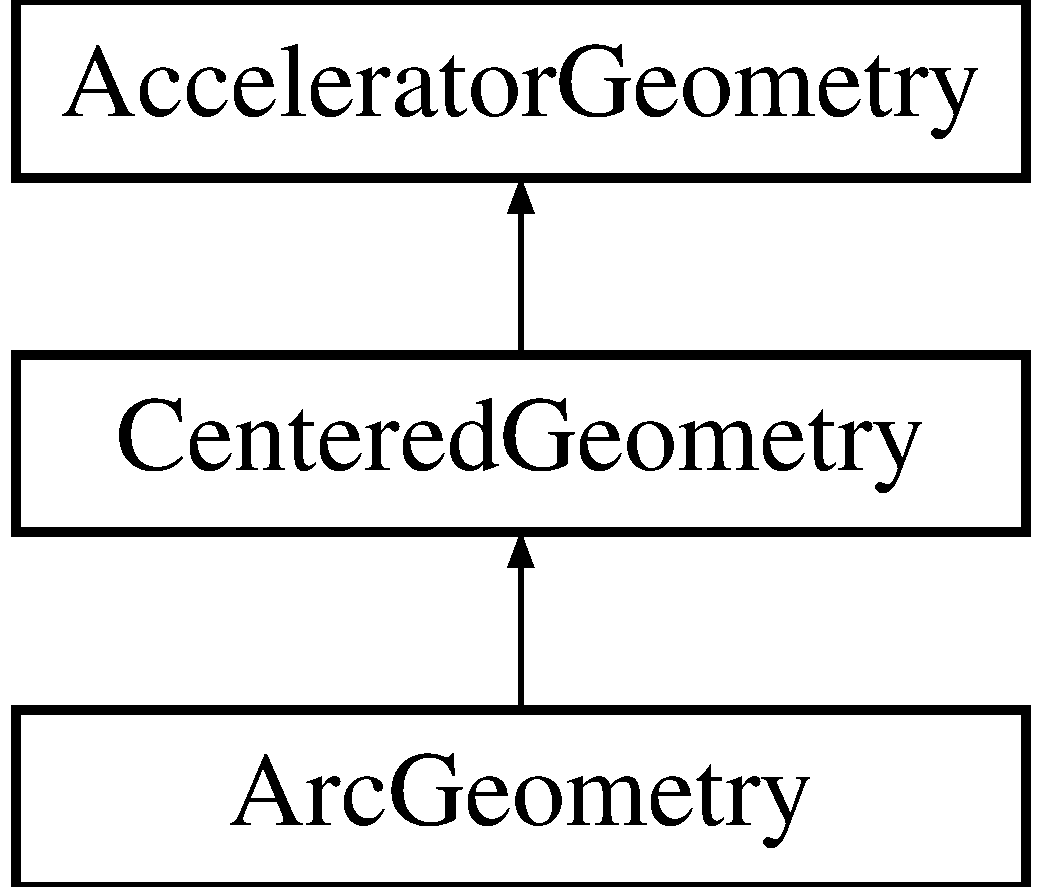
\includegraphics[height=3.000000cm]{classArcGeometry}
\end{center}
\end{figure}
\subsection*{Public Member Functions}
\begin{DoxyCompactItemize}
\item 
\mbox{\Hypertarget{classArcGeometry_ab2831b04e62efcd40d0f2f14985828f0}\label{classArcGeometry_ab2831b04e62efcd40d0f2f14985828f0}} 
{\bfseries Arc\+Geometry} (double l, double curv)
\item 
\mbox{\Hypertarget{classArcGeometry_a0a285ce6fb24e94c734be8529f33f023}\label{classArcGeometry_a0a285ce6fb24e94c734be8529f33f023}} 
double {\bfseries Get\+Curvature} () const
\item 
\mbox{\Hypertarget{classArcGeometry_ab8816547aaf9ef2993af2daee51758e1}\label{classArcGeometry_ab8816547aaf9ef2993af2daee51758e1}} 
double {\bfseries Get\+Angle} () const
\item 
virtual \hyperlink{classTransform3D}{Transform3D} \hyperlink{classArcGeometry_affd534869f6f79b4b271a07b51145b7c}{Get\+Geometry\+Transform} (double s0, double s) const
\item 
virtual \hyperlink{classTransform3D}{Transform3D} \hyperlink{classArcGeometry_aaa665b9dba9b879f38cb5e4a97967533}{Get\+Geometry\+Transform} (\hyperlink{classAcceleratorGeometry_a5c1661938176102f235836f5a8be6034}{Boundary\+Plane} p) const
\item 
virtual \hyperlink{classTransform3D}{Transform3D} \hyperlink{classArcGeometry_aceed7dd7294528003f4bd9f624ef6c9b}{Get\+Total\+Geometry\+Transform} () const
\item 
\mbox{\Hypertarget{classArcGeometry_afced48a170ee36a2a87277148e3617c1}\label{classArcGeometry_afced48a170ee36a2a87277148e3617c1}} 
void {\bfseries Set\+Curvature} (double curv)
\item 
\mbox{\Hypertarget{classArcGeometry_a4a41e90600cbd47c308df598438e99a0}\label{classArcGeometry_a4a41e90600cbd47c308df598438e99a0}} 
void {\bfseries Set\+Tilt} (double t)
\item 
\mbox{\Hypertarget{classArcGeometry_a339d9b840cb94a4aef516989e3149ed2}\label{classArcGeometry_a339d9b840cb94a4aef516989e3149ed2}} 
double {\bfseries Get\+Tilt} () const
\end{DoxyCompactItemize}
\subsection*{Additional Inherited Members}


\subsection{Member Function Documentation}
\mbox{\Hypertarget{classArcGeometry_affd534869f6f79b4b271a07b51145b7c}\label{classArcGeometry_affd534869f6f79b4b271a07b51145b7c}} 
\index{Arc\+Geometry@{Arc\+Geometry}!Get\+Geometry\+Transform@{Get\+Geometry\+Transform}}
\index{Get\+Geometry\+Transform@{Get\+Geometry\+Transform}!Arc\+Geometry@{Arc\+Geometry}}
\subsubsection{\texorpdfstring{Get\+Geometry\+Transform()}{GetGeometryTransform()}\hspace{0.1cm}{\footnotesize\ttfamily [1/2]}}
{\footnotesize\ttfamily \hyperlink{classTransform3D}{Transform3D} Arc\+Geometry\+::\+Get\+Geometry\+Transform (\begin{DoxyParamCaption}\item[{double}]{s0,  }\item[{double}]{s }\end{DoxyParamCaption}) const\hspace{0.3cm}{\ttfamily [virtual]}}

Return the three-\/dimensional transformation from the frame at s0 to the frame at s. s and s0 are in the geometry\textquotesingle{}s s-\/frame, and must be within the geometry extents. 
\begin{DoxyParams}[1]{Parameters}
\mbox{\tt in}  & {\em s0} & The location at which the transform should be evalutated from. \\
\hline
\mbox{\tt in}  & {\em s} & The location at which the transform should be evalutated to. \\
\hline
\end{DoxyParams}

\begin{DoxyExceptions}{Exceptions}
{\em Throws} & a Beyond\+Extent exception if the requested s values are outside the geometry extent. \\
\hline
\end{DoxyExceptions}
\begin{DoxyReturn}{Returns}
The 3D transformation from the entrance to the exit of this geometry. 
\end{DoxyReturn}


Implements \hyperlink{classAcceleratorGeometry_abf9c17cd1f84ac3e41973c85a65004de}{Accelerator\+Geometry}.

\mbox{\Hypertarget{classArcGeometry_aaa665b9dba9b879f38cb5e4a97967533}\label{classArcGeometry_aaa665b9dba9b879f38cb5e4a97967533}} 
\index{Arc\+Geometry@{Arc\+Geometry}!Get\+Geometry\+Transform@{Get\+Geometry\+Transform}}
\index{Get\+Geometry\+Transform@{Get\+Geometry\+Transform}!Arc\+Geometry@{Arc\+Geometry}}
\subsubsection{\texorpdfstring{Get\+Geometry\+Transform()}{GetGeometryTransform()}\hspace{0.1cm}{\footnotesize\ttfamily [2/2]}}
{\footnotesize\ttfamily \hyperlink{classTransform3D}{Transform3D} Arc\+Geometry\+::\+Get\+Geometry\+Transform (\begin{DoxyParamCaption}\item[{\hyperlink{classAcceleratorGeometry_a5c1661938176102f235836f5a8be6034}{Boundary\+Plane}}]{p }\end{DoxyParamCaption}) const\hspace{0.3cm}{\ttfamily [virtual]}}

Returns the transformation from the geometry origin to the specified boundary plane. 
\begin{DoxyParams}[1]{Parameters}
\mbox{\tt in}  & {\em p} & The chosen Boundary\+Plane \\
\hline
\end{DoxyParams}
\begin{DoxyReturn}{Returns}
The 3D transformation from the geometry origin to a specified boundary plane (extrance or exit). 
\end{DoxyReturn}


Implements \hyperlink{classAcceleratorGeometry_af26654f89c4bff1b516d2c6d6bb68871}{Accelerator\+Geometry}.

\mbox{\Hypertarget{classArcGeometry_aceed7dd7294528003f4bd9f624ef6c9b}\label{classArcGeometry_aceed7dd7294528003f4bd9f624ef6c9b}} 
\index{Arc\+Geometry@{Arc\+Geometry}!Get\+Total\+Geometry\+Transform@{Get\+Total\+Geometry\+Transform}}
\index{Get\+Total\+Geometry\+Transform@{Get\+Total\+Geometry\+Transform}!Arc\+Geometry@{Arc\+Geometry}}
\subsubsection{\texorpdfstring{Get\+Total\+Geometry\+Transform()}{GetTotalGeometryTransform()}}
{\footnotesize\ttfamily \hyperlink{classTransform3D}{Transform3D} Arc\+Geometry\+::\+Get\+Total\+Geometry\+Transform (\begin{DoxyParamCaption}{ }\end{DoxyParamCaption}) const\hspace{0.3cm}{\ttfamily [virtual]}}

Returns the transformation from the entrance plane frame to the exit plane frame. \begin{DoxyReturn}{Returns}
The 3D transformation from the entrance to the exit of this geometry. 
\end{DoxyReturn}


Reimplemented from \hyperlink{classAcceleratorGeometry_a9bffb8262fc3b28195e1e25fbfb2b8ba}{Accelerator\+Geometry}.



The documentation for this class was generated from the following files\+:\begin{DoxyCompactItemize}
\item 
/home/fallon/git/merlin-\/cmake/\+Merlin/Arc\+Geometry.\+h\item 
/home/fallon/git/merlin-\/cmake/\+Merlin/Arc\+Geometry.\+cpp\end{DoxyCompactItemize}

\hypertarget{classATL2D}{}\section{A\+T\+L2D Class Reference}
\label{classATL2D}\index{A\+T\+L2D@{A\+T\+L2D}}
\subsection*{Public Types}
\begin{DoxyCompactItemize}
\item 
\mbox{\Hypertarget{classATL2D_a9da4a65fa21af08f0afcab8060ed43da}\label{classATL2D_a9da4a65fa21af08f0afcab8060ed43da}} 
enum {\bfseries A\+T\+L\+Mode} \{ {\bfseries increment}, 
{\bfseries absolute}
 \}
\end{DoxyCompactItemize}
\subsection*{Public Member Functions}
\begin{DoxyCompactItemize}
\item 
\mbox{\Hypertarget{classATL2D_a508d8ea70eba237e929dedb2f56a18ac}\label{classATL2D_a508d8ea70eba237e929dedb2f56a18ac}} 
{\bfseries A\+T\+L2D} (double anA, const Accelerator\+Support\+List \&supports, const \hyperlink{classTVec2D}{Point2D} ref\+Point=\hyperlink{classTVec2D}{Point2D}(0, 0), ifstream $\ast$evec\+T\+File=nullptr, ifstream $\ast$eval\+File=nullptr)
\item 
\mbox{\Hypertarget{classATL2D_ac63fb4a4064f82f12962809ba42dc876}\label{classATL2D_ac63fb4a4064f82f12962809ba42dc876}} 
void {\bfseries Reset} ()
\item 
\mbox{\Hypertarget{classATL2D_ab89d4ac472d16428f05862da37c6a775}\label{classATL2D_ab89d4ac472d16428f05862da37c6a775}} 
double {\bfseries Do\+Step} (double dt)
\item 
\mbox{\Hypertarget{classATL2D_a82db2b069d935cbd55a94b95036db641}\label{classATL2D_a82db2b069d935cbd55a94b95036db641}} 
void {\bfseries Record\+Offsets} (std\+::ostream \&os) const
\item 
\mbox{\Hypertarget{classATL2D_a71428bd01bf47b361b09ff410851bbe4}\label{classATL2D_a71428bd01bf47b361b09ff410851bbe4}} 
double {\bfseries Get\+Time} () const
\item 
\mbox{\Hypertarget{classATL2D_a06c110e3eac5943a4dc811a1b8c0c312}\label{classATL2D_a06c110e3eac5943a4dc811a1b8c0c312}} 
void {\bfseries Set\+Random\+Seed} (unsigned int nseed)
\item 
\mbox{\Hypertarget{classATL2D_ac1adf7295344bbab22b6eccfeee7538e}\label{classATL2D_ac1adf7295344bbab22b6eccfeee7538e}} 
unsigned int {\bfseries Get\+Random\+Seed} () const
\item 
\mbox{\Hypertarget{classATL2D_a1ea2e3c38ce8345fc3331cbe7e87ab4a}\label{classATL2D_a1ea2e3c38ce8345fc3331cbe7e87ab4a}} 
void {\bfseries Reset\+Random\+Seed} ()
\item 
\mbox{\Hypertarget{classATL2D_a017e4c5e7e34b0320812ba7757bce60a}\label{classATL2D_a017e4c5e7e34b0320812ba7757bce60a}} 
bool {\bfseries Set\+A\+T\+L\+Mode} (const A\+T\+L\+Mode mode)
\item 
\mbox{\Hypertarget{classATL2D_aa96730144a50df16e195e61a4eeb9380}\label{classATL2D_aa96730144a50df16e195e61a4eeb9380}} 
bool {\bfseries Set\+Vibration} (const double vrms)
\item 
\mbox{\Hypertarget{classATL2D_adf994271afcce311a67c63fe094a3423}\label{classATL2D_adf994271afcce311a67c63fe094a3423}} 
void {\bfseries Record\+Eigen\+System} (ofstream $\ast$evec\+T\+File, ofstream $\ast$eval\+File)
\end{DoxyCompactItemize}


The documentation for this class was generated from the following files\+:\begin{DoxyCompactItemize}
\item 
/home/fallon/git/merlin-\/cmake/\+Merlin/A\+T\+L2\+D.\+h\item 
/home/fallon/git/merlin-\/cmake/\+Merlin/A\+T\+L2\+D.\+cpp\end{DoxyCompactItemize}

\hypertarget{classTBunchCMPTracker_1_1B__Integrator}{}\section{T\+Bunch\+C\+M\+P\+Tracker$<$ \+\_\+B $>$\+:\+:B\+\_\+\+Integrator Class Reference}
\label{classTBunchCMPTracker_1_1B__Integrator}\index{T\+Bunch\+C\+M\+P\+Tracker$<$ \+\_\+\+B $>$\+::\+B\+\_\+\+Integrator@{T\+Bunch\+C\+M\+P\+Tracker$<$ \+\_\+\+B $>$\+::\+B\+\_\+\+Integrator}}
Inheritance diagram for T\+Bunch\+C\+M\+P\+Tracker$<$ \+\_\+B $>$\+:\+:B\+\_\+\+Integrator\+:\begin{figure}[H]
\begin{center}
\leavevmode
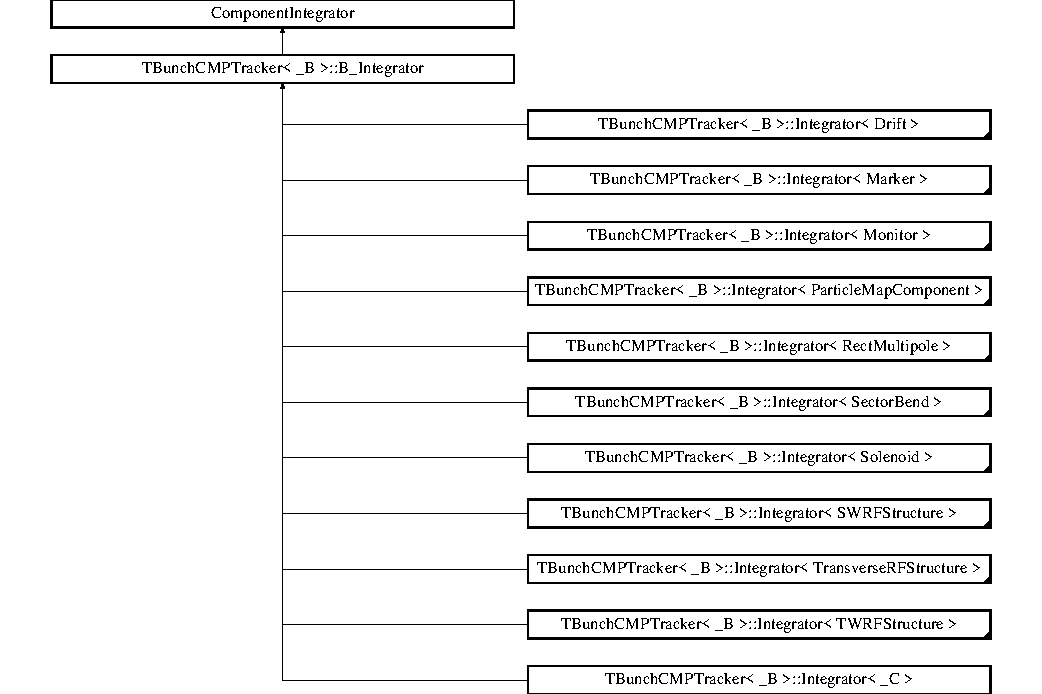
\includegraphics[height=9.333334cm]{classTBunchCMPTracker_1_1B__Integrator}
\end{center}
\end{figure}
\subsection*{Public Member Functions}
\begin{DoxyCompactItemize}
\item 
\mbox{\Hypertarget{classTBunchCMPTracker_1_1B__Integrator_ad7015d6e3d90070283aac44ac1e9555b}\label{classTBunchCMPTracker_1_1B__Integrator_ad7015d6e3d90070283aac44ac1e9555b}} 
void {\bfseries Set\+Bunch} (\+\_\+B \&a\+Bunch)
\item 
\mbox{\Hypertarget{classTBunchCMPTracker_1_1B__Integrator_a5bfcc6e762a41c0660d6884d980b72b4}\label{classTBunchCMPTracker_1_1B__Integrator_a5bfcc6e762a41c0660d6884d980b72b4}} 
virtual double {\bfseries Track} (double ds)
\end{DoxyCompactItemize}
\subsection*{Protected Attributes}
\begin{DoxyCompactItemize}
\item 
\mbox{\Hypertarget{classTBunchCMPTracker_1_1B__Integrator_afe34e0eab12b5077fa154034943f3ea5}\label{classTBunchCMPTracker_1_1B__Integrator_afe34e0eab12b5077fa154034943f3ea5}} 
\+\_\+B $\ast$ {\bfseries current\+Bunch}
\end{DoxyCompactItemize}
\subsection*{Additional Inherited Members}


The documentation for this class was generated from the following file\+:\begin{DoxyCompactItemize}
\item 
/home/fallon/git/merlin-\/cmake/\+Merlin/Component\+Tracker.\+h\end{DoxyCompactItemize}

\hypertarget{structMADKeyMap_1_1bad__key}{}\section{M\+A\+D\+Key\+Map\+:\+:bad\+\_\+key Struct Reference}
\label{structMADKeyMap_1_1bad__key}\index{M\+A\+D\+Key\+Map\+::bad\+\_\+key@{M\+A\+D\+Key\+Map\+::bad\+\_\+key}}


The documentation for this struct was generated from the following file\+:\begin{DoxyCompactItemize}
\item 
/home/fallon/git/merlin-\/cmake/\+Merlin/M\+A\+D\+Key\+Map.\+h\end{DoxyCompactItemize}

\hypertarget{classInterpolation_1_1BadRange}{}\section{Interpolation\+:\+:Bad\+Range Class Reference}
\label{classInterpolation_1_1BadRange}\index{Interpolation\+::\+Bad\+Range@{Interpolation\+::\+Bad\+Range}}
Inheritance diagram for Interpolation\+:\+:Bad\+Range\+:\begin{figure}[H]
\begin{center}
\leavevmode
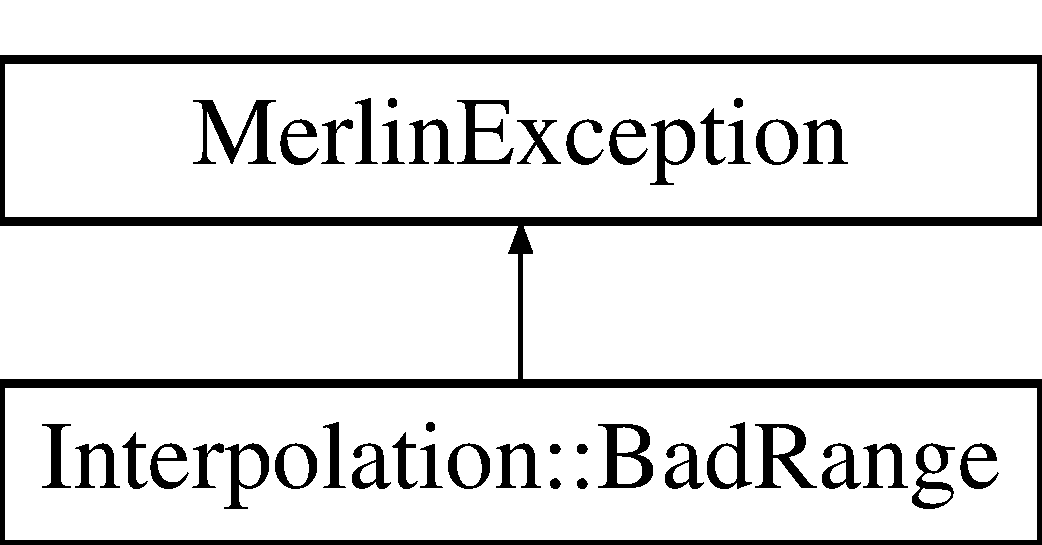
\includegraphics[height=2.000000cm]{classInterpolation_1_1BadRange}
\end{center}
\end{figure}
\subsection*{Public Member Functions}
\begin{DoxyCompactItemize}
\item 
\mbox{\Hypertarget{classInterpolation_1_1BadRange_a2ee312bf850dbd51ff47d7114644efb3}\label{classInterpolation_1_1BadRange_a2ee312bf850dbd51ff47d7114644efb3}} 
{\bfseries Bad\+Range} (double x, const \hyperlink{classNumericalRange}{Float\+Range} \&r)
\end{DoxyCompactItemize}
\subsection*{Public Attributes}
\begin{DoxyCompactItemize}
\item 
\mbox{\Hypertarget{classInterpolation_1_1BadRange_a2c2abea652f02f8858eaa6c290674785}\label{classInterpolation_1_1BadRange_a2c2abea652f02f8858eaa6c290674785}} 
double {\bfseries value}
\item 
\mbox{\Hypertarget{classInterpolation_1_1BadRange_a10104044db3ab00fb715e68a7c28627a}\label{classInterpolation_1_1BadRange_a10104044db3ab00fb715e68a7c28627a}} 
\hyperlink{classNumericalRange}{Float\+Range} {\bfseries valid\+\_\+range}
\end{DoxyCompactItemize}
\subsection*{Additional Inherited Members}


The documentation for this class was generated from the following files\+:\begin{DoxyCompactItemize}
\item 
/home/fallon/git/merlin-\/cmake/\+Merlin/Interpolation.\+h\item 
/home/fallon/git/merlin-\/cmake/\+Merlin/Interpolation.\+cpp\end{DoxyCompactItemize}

\hypertarget{classAcceleratorModel_1_1BadRange}{}\section{Accelerator\+Model\+:\+:Bad\+Range Class Reference}
\label{classAcceleratorModel_1_1BadRange}\index{Accelerator\+Model\+::\+Bad\+Range@{Accelerator\+Model\+::\+Bad\+Range}}


{\ttfamily \#include $<$Accelerator\+Model.\+h$>$}

Inheritance diagram for Accelerator\+Model\+:\+:Bad\+Range\+:\begin{figure}[H]
\begin{center}
\leavevmode
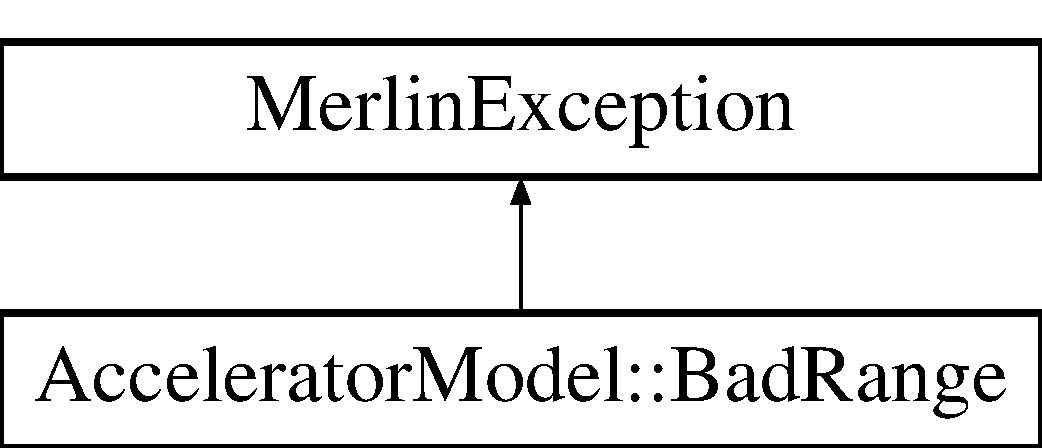
\includegraphics[height=2.000000cm]{classAcceleratorModel_1_1BadRange}
\end{center}
\end{figure}
\subsection*{Additional Inherited Members}


\subsection{Detailed Description}
Exception class for Get\+Beamline functions 

The documentation for this class was generated from the following file\+:\begin{DoxyCompactItemize}
\item 
/home/fallon/git/merlin-\/cmake/\+Merlin/Accelerator\+Model.\+h\end{DoxyCompactItemize}

\hypertarget{classbasic__echo__ostream}{}\section{basic\+\_\+echo\+\_\+ostream$<$ T, Tr $>$ Class Template Reference}
\label{classbasic__echo__ostream}\index{basic\+\_\+echo\+\_\+ostream$<$ T, Tr $>$@{basic\+\_\+echo\+\_\+ostream$<$ T, Tr $>$}}
Inheritance diagram for basic\+\_\+echo\+\_\+ostream$<$ T, Tr $>$\+:\begin{figure}[H]
\begin{center}
\leavevmode
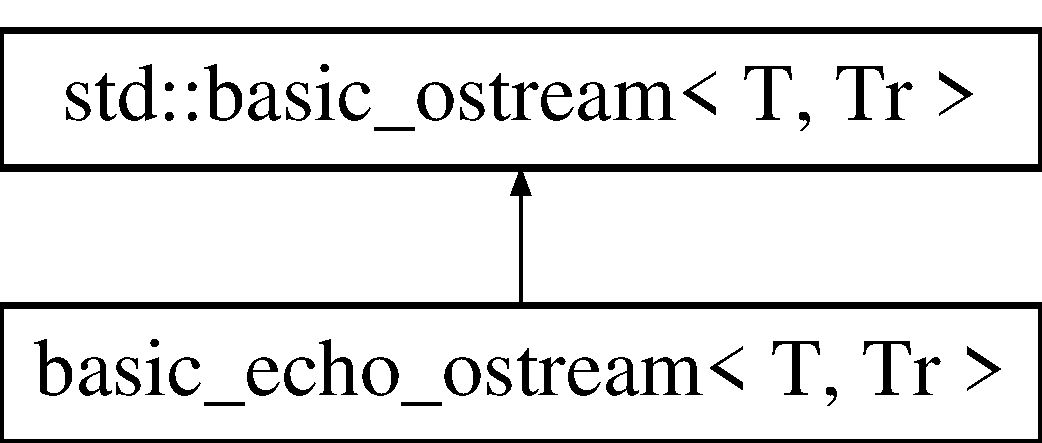
\includegraphics[height=2.000000cm]{classbasic__echo__ostream}
\end{center}
\end{figure}
\subsection*{Classes}
\begin{DoxyCompactItemize}
\item 
class \hyperlink{classbasic__echo__ostream_1_1echo__streambuf}{echo\+\_\+streambuf}
\end{DoxyCompactItemize}
\subsection*{Public Member Functions}
\begin{DoxyCompactItemize}
\item 
\mbox{\Hypertarget{classbasic__echo__ostream_adef0dcc882ca8eb0b503ffcdc4bf2958}\label{classbasic__echo__ostream_adef0dcc882ca8eb0b503ffcdc4bf2958}} 
{\bfseries basic\+\_\+echo\+\_\+ostream} (std\+::basic\+\_\+ostream$<$ T, Tr $>$ \&first, std\+::basic\+\_\+ostream$<$ T, Tr $>$ \&second)
\end{DoxyCompactItemize}


The documentation for this class was generated from the following file\+:\begin{DoxyCompactItemize}
\item 
/home/fallon/git/merlin-\/cmake/\+Merlin/echo\+\_\+ostream.\+h\end{DoxyCompactItemize}

\hypertarget{classBeamData}{}\section{Beam\+Data Class Reference}
\label{classBeamData}\index{Beam\+Data@{Beam\+Data}}
\subsection*{Public Member Functions}
\begin{DoxyCompactItemize}
\item 
\mbox{\Hypertarget{classBeamData_ac4ff99b7261467265ac3912e470d7d7e}\label{classBeamData_ac4ff99b7261467265ac3912e470d7d7e}} 
bool {\bfseries ok} () const
\item 
\mbox{\Hypertarget{classBeamData_a4a8455b1f348e72dd5d3bb8e6b2c80f8}\label{classBeamData_a4a8455b1f348e72dd5d3bb8e6b2c80f8}} 
double {\bfseries gamma\+\_\+x} () const
\item 
\mbox{\Hypertarget{classBeamData_a6c4c04483593a1d5fb079c013d233c85}\label{classBeamData_a6c4c04483593a1d5fb079c013d233c85}} 
double {\bfseries gamma\+\_\+y} () const
\item 
\mbox{\Hypertarget{classBeamData_ae731a1497167bff681c4bc07034b6ed8}\label{classBeamData_ae731a1497167bff681c4bc07034b6ed8}} 
double {\bfseries sigma\+\_\+x} () const
\item 
\mbox{\Hypertarget{classBeamData_a1d6ef4b768a88bf4540fc88850f1c674}\label{classBeamData_a1d6ef4b768a88bf4540fc88850f1c674}} 
double {\bfseries sigma\+\_\+y} () const
\item 
\mbox{\Hypertarget{classBeamData_a7e16ee61642e673914a6e7a48910b1b4}\label{classBeamData_a7e16ee61642e673914a6e7a48910b1b4}} 
double {\bfseries sigma\+\_\+xp} () const
\item 
\mbox{\Hypertarget{classBeamData_aaf10e290313f13ef8eafd741c2950652}\label{classBeamData_aaf10e290313f13ef8eafd741c2950652}} 
double {\bfseries sigma\+\_\+yp} () const
\end{DoxyCompactItemize}
\subsection*{Public Attributes}
\begin{DoxyCompactItemize}
\item 
\mbox{\Hypertarget{classBeamData_a2876f0ddc250924cea86ceb37f60b458}\label{classBeamData_a2876f0ddc250924cea86ceb37f60b458}} 
double {\bfseries beta\+\_\+x}
\item 
\mbox{\Hypertarget{classBeamData_a73def6d2b4da1e6faeb4ed8cb199d5cd}\label{classBeamData_a73def6d2b4da1e6faeb4ed8cb199d5cd}} 
double {\bfseries beta\+\_\+y}
\item 
\mbox{\Hypertarget{classBeamData_a6276d7cdbdf1ce3f9440779d519e11f1}\label{classBeamData_a6276d7cdbdf1ce3f9440779d519e11f1}} 
double {\bfseries alpha\+\_\+x}
\item 
\mbox{\Hypertarget{classBeamData_a50c29f6199a44ff8e4edb3ad1e200e2f}\label{classBeamData_a50c29f6199a44ff8e4edb3ad1e200e2f}} 
double {\bfseries alpha\+\_\+y}
\item 
\mbox{\Hypertarget{classBeamData_ab902ce8e07049d0cb53330abe8451106}\label{classBeamData_ab902ce8e07049d0cb53330abe8451106}} 
double {\bfseries emit\+\_\+x}
\item 
\mbox{\Hypertarget{classBeamData_a51a6a5027d314a721e3ba9465db92114}\label{classBeamData_a51a6a5027d314a721e3ba9465db92114}} 
double {\bfseries emit\+\_\+y}
\item 
\mbox{\Hypertarget{classBeamData_ab8d029d4060ee5412a1e106a5c51c401}\label{classBeamData_ab8d029d4060ee5412a1e106a5c51c401}} 
double {\bfseries sig\+\_\+dp}
\item 
\mbox{\Hypertarget{classBeamData_a933ca595f133a07e52a2b72e308e0219}\label{classBeamData_a933ca595f133a07e52a2b72e308e0219}} 
double {\bfseries sig\+\_\+z}
\item 
\mbox{\Hypertarget{classBeamData_a212c9818f67e05d2d14e1f33dafb4c62}\label{classBeamData_a212c9818f67e05d2d14e1f33dafb4c62}} 
double {\bfseries x0}
\item 
\mbox{\Hypertarget{classBeamData_a08315a47b36fa979cae2999c0d330f40}\label{classBeamData_a08315a47b36fa979cae2999c0d330f40}} 
double {\bfseries xp0}
\item 
\mbox{\Hypertarget{classBeamData_a9589ce6ab4bc4a3bba7318016e8573e4}\label{classBeamData_a9589ce6ab4bc4a3bba7318016e8573e4}} 
double {\bfseries y0}
\item 
\mbox{\Hypertarget{classBeamData_a5ac747b13988d365f0a107120cece249}\label{classBeamData_a5ac747b13988d365f0a107120cece249}} 
double {\bfseries yp0}
\item 
\mbox{\Hypertarget{classBeamData_aaf403be214b8a4edfe85b59d1b023a8e}\label{classBeamData_aaf403be214b8a4edfe85b59d1b023a8e}} 
double {\bfseries ct0}
\item 
\mbox{\Hypertarget{classBeamData_a638cbb6fbd46a12a44492b88eb94016a}\label{classBeamData_a638cbb6fbd46a12a44492b88eb94016a}} 
double {\bfseries p0}
\item 
\mbox{\Hypertarget{classBeamData_a4bb725a9908083b6a8d2e09db5bae93f}\label{classBeamData_a4bb725a9908083b6a8d2e09db5bae93f}} 
double {\bfseries c\+\_\+xy}
\item 
\mbox{\Hypertarget{classBeamData_a2dd71a41d153b6724685190826df62f9}\label{classBeamData_a2dd71a41d153b6724685190826df62f9}} 
double {\bfseries c\+\_\+xyp}
\item 
\mbox{\Hypertarget{classBeamData_a2862e30484c8adffe41eac6882fc208f}\label{classBeamData_a2862e30484c8adffe41eac6882fc208f}} 
double {\bfseries c\+\_\+xpy}
\item 
\mbox{\Hypertarget{classBeamData_a2479aaa6b075a182e89bf924323caa41}\label{classBeamData_a2479aaa6b075a182e89bf924323caa41}} 
double {\bfseries c\+\_\+xpyp}
\item 
\mbox{\Hypertarget{classBeamData_a9f6987dae37a0c6d13f701b3af6a1286}\label{classBeamData_a9f6987dae37a0c6d13f701b3af6a1286}} 
double {\bfseries Dx}
\item 
\mbox{\Hypertarget{classBeamData_a9f4efcc8951fd3a7045a4291e6ae0004}\label{classBeamData_a9f4efcc8951fd3a7045a4291e6ae0004}} 
double {\bfseries Dxp}
\item 
\mbox{\Hypertarget{classBeamData_ad3ed1445bc60061ec94ea986d1723d5c}\label{classBeamData_ad3ed1445bc60061ec94ea986d1723d5c}} 
double {\bfseries Dy}
\item 
\mbox{\Hypertarget{classBeamData_a93ebce129459bf8650648047c6924d5d}\label{classBeamData_a93ebce129459bf8650648047c6924d5d}} 
double {\bfseries Dyp}
\item 
\mbox{\Hypertarget{classBeamData_ac779e54adef56269a2a21ec3cfb18211}\label{classBeamData_ac779e54adef56269a2a21ec3cfb18211}} 
double {\bfseries charge}
\end{DoxyCompactItemize}


The documentation for this class was generated from the following file\+:\begin{DoxyCompactItemize}
\item 
/home/fallon/git/merlin-\/cmake/\+Merlin/Beam\+Data.\+h\end{DoxyCompactItemize}

\hypertarget{classAcceleratorModel_1_1Beamline}{}\section{Accelerator\+Model\+:\+:Beamline Class Reference}
\label{classAcceleratorModel_1_1Beamline}\index{Accelerator\+Model\+::\+Beamline@{Accelerator\+Model\+::\+Beamline}}


{\ttfamily \#include $<$Accelerator\+Model.\+h$>$}

\subsection*{Classes}
\begin{DoxyCompactItemize}
\item 
class \hyperlink{classAcceleratorModel_1_1Beamline_1_1TRK}{T\+RK}
\end{DoxyCompactItemize}
\subsection*{Public Member Functions}
\begin{DoxyCompactItemize}
\item 
\mbox{\Hypertarget{classAcceleratorModel_1_1Beamline_a3474fa3882d6c64f585fd1d31f33bbab}\label{classAcceleratorModel_1_1Beamline_a3474fa3882d6c64f585fd1d31f33bbab}} 
{\bfseries Beamline} (Beamline\+Iterator fst, Beamline\+Iterator lst, Index fst\+\_\+i, Index lst\+\_\+i)
\item 
bool \hyperlink{classAcceleratorModel_1_1Beamline_acbb49274dda0a8bbc7daa0a3a845508e}{Is\+Reversed} ()
\item 
{\footnotesize template$<$class T $>$ }\\T \& \hyperlink{classAcceleratorModel_1_1Beamline_af48fc0105707f1b09e5b343ffa829854}{Track} (T \&tobj)
\item 
Beamline\+Iterator \hyperlink{classAcceleratorModel_1_1Beamline_a1cccebda06318f2ed33b12a19cf7acba}{begin} ()
\item 
Const\+Beamline\+Iterator \hyperlink{classAcceleratorModel_1_1Beamline_a1580e7da07af01517c3d552464b267ed}{begin} () const
\item 
Beamline\+Iterator \hyperlink{classAcceleratorModel_1_1Beamline_a190fe2e2aeca28999af7b07beea84d60}{end} ()
\item 
Const\+Beamline\+Iterator \hyperlink{classAcceleratorModel_1_1Beamline_af0f0f0244723579b42b2e893a2273ea4}{end} () const
\item 
\hyperlink{classComponentFrame}{Component\+Frame} \& \hyperlink{classAcceleratorModel_1_1Beamline_a56c50274a705cd04a6059ffe384c897a}{First} ()
\item 
const \hyperlink{classComponentFrame}{Component\+Frame} \& \hyperlink{classAcceleratorModel_1_1Beamline_aa1a924ddf820afe8c914a4ff03893bc3}{First} () const
\item 
\hyperlink{classComponentFrame}{Component\+Frame} \& \hyperlink{classAcceleratorModel_1_1Beamline_aebb83c56d1f6b346f08f29cad78a4896}{Last} ()
\item 
const \hyperlink{classComponentFrame}{Component\+Frame} \& \hyperlink{classAcceleratorModel_1_1Beamline_a3d9e8887cc1b7cfbc0d497f749af3950}{Last} () const
\item 
Index \hyperlink{classAcceleratorModel_1_1Beamline_a67b5d69c05315b04b3f0fb4c28fe40a9}{first\+\_\+index} () const
\item 
Index \hyperlink{classAcceleratorModel_1_1Beamline_a5e20d3e994c496cf16744d0a54bd26a0}{last\+\_\+index} () const
\end{DoxyCompactItemize}


\subsection{Detailed Description}
Represents the complete or contiguous sub-\/section of the accelerator lattice. 

\subsection{Member Function Documentation}
\mbox{\Hypertarget{classAcceleratorModel_1_1Beamline_a1cccebda06318f2ed33b12a19cf7acba}\label{classAcceleratorModel_1_1Beamline_a1cccebda06318f2ed33b12a19cf7acba}} 
\index{Accelerator\+Model\+::\+Beamline@{Accelerator\+Model\+::\+Beamline}!begin@{begin}}
\index{begin@{begin}!Accelerator\+Model\+::\+Beamline@{Accelerator\+Model\+::\+Beamline}}
\subsubsection{\texorpdfstring{begin()}{begin()}\hspace{0.1cm}{\footnotesize\ttfamily [1/2]}}
{\footnotesize\ttfamily Beamline\+Iterator Accelerator\+Model\+::\+Beamline\+::begin (\begin{DoxyParamCaption}{ }\end{DoxyParamCaption})\hspace{0.3cm}{\ttfamily [inline]}}

Standard library type iterator accessors. Gets a Beamline\+Iterator pointing to the first element in the \hyperlink{classAcceleratorModel_1_1Beamline}{Beamline}. \begin{DoxyReturn}{Returns}
A Beamline\+Iterator pointing to the first element in the \hyperlink{classAcceleratorModel_1_1Beamline}{Beamline}. 
\end{DoxyReturn}
\mbox{\Hypertarget{classAcceleratorModel_1_1Beamline_a1580e7da07af01517c3d552464b267ed}\label{classAcceleratorModel_1_1Beamline_a1580e7da07af01517c3d552464b267ed}} 
\index{Accelerator\+Model\+::\+Beamline@{Accelerator\+Model\+::\+Beamline}!begin@{begin}}
\index{begin@{begin}!Accelerator\+Model\+::\+Beamline@{Accelerator\+Model\+::\+Beamline}}
\subsubsection{\texorpdfstring{begin()}{begin()}\hspace{0.1cm}{\footnotesize\ttfamily [2/2]}}
{\footnotesize\ttfamily Const\+Beamline\+Iterator Accelerator\+Model\+::\+Beamline\+::begin (\begin{DoxyParamCaption}{ }\end{DoxyParamCaption}) const\hspace{0.3cm}{\ttfamily [inline]}}

Gets a const Beamline\+Iterator pointing to the first element in the \hyperlink{classAcceleratorModel_1_1Beamline}{Beamline}. \begin{DoxyReturn}{Returns}
A const Beamline\+Iterator pointing to the first element in the \hyperlink{classAcceleratorModel_1_1Beamline}{Beamline}. 
\end{DoxyReturn}
\mbox{\Hypertarget{classAcceleratorModel_1_1Beamline_a190fe2e2aeca28999af7b07beea84d60}\label{classAcceleratorModel_1_1Beamline_a190fe2e2aeca28999af7b07beea84d60}} 
\index{Accelerator\+Model\+::\+Beamline@{Accelerator\+Model\+::\+Beamline}!end@{end}}
\index{end@{end}!Accelerator\+Model\+::\+Beamline@{Accelerator\+Model\+::\+Beamline}}
\subsubsection{\texorpdfstring{end()}{end()}\hspace{0.1cm}{\footnotesize\ttfamily [1/2]}}
{\footnotesize\ttfamily Beamline\+Iterator Accelerator\+Model\+::\+Beamline\+::end (\begin{DoxyParamCaption}{ }\end{DoxyParamCaption})\hspace{0.3cm}{\ttfamily [inline]}}

Gets a Beamline\+Iterator pointing to the end of the \hyperlink{classAcceleratorModel_1_1Beamline}{Beamline}. \begin{DoxyReturn}{Returns}
A Beamline\+Iterator pointing to the end of the \hyperlink{classAcceleratorModel_1_1Beamline}{Beamline}. 
\end{DoxyReturn}
\mbox{\Hypertarget{classAcceleratorModel_1_1Beamline_af0f0f0244723579b42b2e893a2273ea4}\label{classAcceleratorModel_1_1Beamline_af0f0f0244723579b42b2e893a2273ea4}} 
\index{Accelerator\+Model\+::\+Beamline@{Accelerator\+Model\+::\+Beamline}!end@{end}}
\index{end@{end}!Accelerator\+Model\+::\+Beamline@{Accelerator\+Model\+::\+Beamline}}
\subsubsection{\texorpdfstring{end()}{end()}\hspace{0.1cm}{\footnotesize\ttfamily [2/2]}}
{\footnotesize\ttfamily Const\+Beamline\+Iterator Accelerator\+Model\+::\+Beamline\+::end (\begin{DoxyParamCaption}{ }\end{DoxyParamCaption}) const\hspace{0.3cm}{\ttfamily [inline]}}

Gets a const Beamline\+Iterator pointing to the end of the \hyperlink{classAcceleratorModel_1_1Beamline}{Beamline}. \begin{DoxyReturn}{Returns}
A const Beamline\+Iterator pointing to the end of the \hyperlink{classAcceleratorModel_1_1Beamline}{Beamline}. 
\end{DoxyReturn}
\mbox{\Hypertarget{classAcceleratorModel_1_1Beamline_a56c50274a705cd04a6059ffe384c897a}\label{classAcceleratorModel_1_1Beamline_a56c50274a705cd04a6059ffe384c897a}} 
\index{Accelerator\+Model\+::\+Beamline@{Accelerator\+Model\+::\+Beamline}!First@{First}}
\index{First@{First}!Accelerator\+Model\+::\+Beamline@{Accelerator\+Model\+::\+Beamline}}
\subsubsection{\texorpdfstring{First()}{First()}\hspace{0.1cm}{\footnotesize\ttfamily [1/2]}}
{\footnotesize\ttfamily \hyperlink{classComponentFrame}{Component\+Frame}\& Accelerator\+Model\+::\+Beamline\+::\+First (\begin{DoxyParamCaption}{ }\end{DoxyParamCaption})\hspace{0.3cm}{\ttfamily [inline]}}

Gets a reference to the first \hyperlink{classComponentFrame}{Component\+Frame}. \begin{DoxyReturn}{Returns}
A reference to the first \hyperlink{classComponentFrame}{Component\+Frame}. 
\end{DoxyReturn}
\mbox{\Hypertarget{classAcceleratorModel_1_1Beamline_aa1a924ddf820afe8c914a4ff03893bc3}\label{classAcceleratorModel_1_1Beamline_aa1a924ddf820afe8c914a4ff03893bc3}} 
\index{Accelerator\+Model\+::\+Beamline@{Accelerator\+Model\+::\+Beamline}!First@{First}}
\index{First@{First}!Accelerator\+Model\+::\+Beamline@{Accelerator\+Model\+::\+Beamline}}
\subsubsection{\texorpdfstring{First()}{First()}\hspace{0.1cm}{\footnotesize\ttfamily [2/2]}}
{\footnotesize\ttfamily const \hyperlink{classComponentFrame}{Component\+Frame}\& Accelerator\+Model\+::\+Beamline\+::\+First (\begin{DoxyParamCaption}{ }\end{DoxyParamCaption}) const\hspace{0.3cm}{\ttfamily [inline]}}

Gets a const reference to the first \hyperlink{classComponentFrame}{Component\+Frame}. \begin{DoxyReturn}{Returns}
A const reference to the first \hyperlink{classComponentFrame}{Component\+Frame}. 
\end{DoxyReturn}
\mbox{\Hypertarget{classAcceleratorModel_1_1Beamline_a67b5d69c05315b04b3f0fb4c28fe40a9}\label{classAcceleratorModel_1_1Beamline_a67b5d69c05315b04b3f0fb4c28fe40a9}} 
\index{Accelerator\+Model\+::\+Beamline@{Accelerator\+Model\+::\+Beamline}!first\+\_\+index@{first\+\_\+index}}
\index{first\+\_\+index@{first\+\_\+index}!Accelerator\+Model\+::\+Beamline@{Accelerator\+Model\+::\+Beamline}}
\subsubsection{\texorpdfstring{first\+\_\+index()}{first\_index()}}
{\footnotesize\ttfamily Index Accelerator\+Model\+::\+Beamline\+::first\+\_\+index (\begin{DoxyParamCaption}{ }\end{DoxyParamCaption}) const\hspace{0.3cm}{\ttfamily [inline]}}

Gets the index of the first element in the \hyperlink{classAcceleratorModel_1_1Beamline}{Beamline}. \begin{DoxyReturn}{Returns}
The index of the first element in the \hyperlink{classAcceleratorModel_1_1Beamline}{Beamline}. 
\end{DoxyReturn}
\mbox{\Hypertarget{classAcceleratorModel_1_1Beamline_acbb49274dda0a8bbc7daa0a3a845508e}\label{classAcceleratorModel_1_1Beamline_acbb49274dda0a8bbc7daa0a3a845508e}} 
\index{Accelerator\+Model\+::\+Beamline@{Accelerator\+Model\+::\+Beamline}!Is\+Reversed@{Is\+Reversed}}
\index{Is\+Reversed@{Is\+Reversed}!Accelerator\+Model\+::\+Beamline@{Accelerator\+Model\+::\+Beamline}}
\subsubsection{\texorpdfstring{Is\+Reversed()}{IsReversed()}}
{\footnotesize\ttfamily bool Accelerator\+Model\+::\+Beamline\+::\+Is\+Reversed (\begin{DoxyParamCaption}{ }\end{DoxyParamCaption})\hspace{0.3cm}{\ttfamily [inline]}}

Checks if the beamline is reversed. \begin{DoxyReturn}{Returns}
Returns a bool set to true if the beamline is reversed. 
\end{DoxyReturn}
\mbox{\Hypertarget{classAcceleratorModel_1_1Beamline_aebb83c56d1f6b346f08f29cad78a4896}\label{classAcceleratorModel_1_1Beamline_aebb83c56d1f6b346f08f29cad78a4896}} 
\index{Accelerator\+Model\+::\+Beamline@{Accelerator\+Model\+::\+Beamline}!Last@{Last}}
\index{Last@{Last}!Accelerator\+Model\+::\+Beamline@{Accelerator\+Model\+::\+Beamline}}
\subsubsection{\texorpdfstring{Last()}{Last()}\hspace{0.1cm}{\footnotesize\ttfamily [1/2]}}
{\footnotesize\ttfamily \hyperlink{classComponentFrame}{Component\+Frame}\& Accelerator\+Model\+::\+Beamline\+::\+Last (\begin{DoxyParamCaption}{ }\end{DoxyParamCaption})\hspace{0.3cm}{\ttfamily [inline]}}

Gets a reference to the last \hyperlink{classComponentFrame}{Component\+Frame}. \begin{DoxyReturn}{Returns}
A reference to the last \hyperlink{classComponentFrame}{Component\+Frame}. 
\end{DoxyReturn}
\mbox{\Hypertarget{classAcceleratorModel_1_1Beamline_a3d9e8887cc1b7cfbc0d497f749af3950}\label{classAcceleratorModel_1_1Beamline_a3d9e8887cc1b7cfbc0d497f749af3950}} 
\index{Accelerator\+Model\+::\+Beamline@{Accelerator\+Model\+::\+Beamline}!Last@{Last}}
\index{Last@{Last}!Accelerator\+Model\+::\+Beamline@{Accelerator\+Model\+::\+Beamline}}
\subsubsection{\texorpdfstring{Last()}{Last()}\hspace{0.1cm}{\footnotesize\ttfamily [2/2]}}
{\footnotesize\ttfamily const \hyperlink{classComponentFrame}{Component\+Frame}\& Accelerator\+Model\+::\+Beamline\+::\+Last (\begin{DoxyParamCaption}{ }\end{DoxyParamCaption}) const\hspace{0.3cm}{\ttfamily [inline]}}

Gets a const reference to the last \hyperlink{classComponentFrame}{Component\+Frame}. \begin{DoxyReturn}{Returns}
A const reference to the last \hyperlink{classComponentFrame}{Component\+Frame}. 
\end{DoxyReturn}
\mbox{\Hypertarget{classAcceleratorModel_1_1Beamline_a5e20d3e994c496cf16744d0a54bd26a0}\label{classAcceleratorModel_1_1Beamline_a5e20d3e994c496cf16744d0a54bd26a0}} 
\index{Accelerator\+Model\+::\+Beamline@{Accelerator\+Model\+::\+Beamline}!last\+\_\+index@{last\+\_\+index}}
\index{last\+\_\+index@{last\+\_\+index}!Accelerator\+Model\+::\+Beamline@{Accelerator\+Model\+::\+Beamline}}
\subsubsection{\texorpdfstring{last\+\_\+index()}{last\_index()}}
{\footnotesize\ttfamily Index Accelerator\+Model\+::\+Beamline\+::last\+\_\+index (\begin{DoxyParamCaption}{ }\end{DoxyParamCaption}) const\hspace{0.3cm}{\ttfamily [inline]}}

Gets the index of the last element in the \hyperlink{classAcceleratorModel_1_1Beamline}{Beamline}. \begin{DoxyReturn}{Returns}
The index of the last element in the \hyperlink{classAcceleratorModel_1_1Beamline}{Beamline}. 
\end{DoxyReturn}
\mbox{\Hypertarget{classAcceleratorModel_1_1Beamline_af48fc0105707f1b09e5b343ffa829854}\label{classAcceleratorModel_1_1Beamline_af48fc0105707f1b09e5b343ffa829854}} 
\index{Accelerator\+Model\+::\+Beamline@{Accelerator\+Model\+::\+Beamline}!Track@{Track}}
\index{Track@{Track}!Accelerator\+Model\+::\+Beamline@{Accelerator\+Model\+::\+Beamline}}
\subsubsection{\texorpdfstring{Track()}{Track()}}
{\footnotesize\ttfamily template$<$class T $>$ \\
T\& Accelerator\+Model\+::\+Beamline\+::\+Track (\begin{DoxyParamCaption}\item[{T \&}]{tobj }\end{DoxyParamCaption})\hspace{0.3cm}{\ttfamily [inline]}}

Template function that iterates the functor object tobj over the \hyperlink{classAcceleratorModel_1_1Beamline}{Beamline}. Returns a reference to tobj on exit. We make use of the \hyperlink{classAcceleratorModel_1_1Beamline_1_1TRK}{T\+RK} wrapper, to avoid the call to tobj\textquotesingle{}s copy constructor

The documentation for this class was generated from the following file\+:\begin{DoxyCompactItemize}
\item 
/home/fallon/git/merlin-\/cmake/\+Merlin/Accelerator\+Model.\+h\end{DoxyCompactItemize}

\hypertarget{classBetatronTunes}{}\section{Betatron\+Tunes Class Reference}
\label{classBetatronTunes}\index{Betatron\+Tunes@{Betatron\+Tunes}}
\subsection*{Public Member Functions}
\begin{DoxyCompactItemize}
\item 
\mbox{\Hypertarget{classBetatronTunes_a267df4288b59cea8533f3b5301732481}\label{classBetatronTunes_a267df4288b59cea8533f3b5301732481}} 
{\bfseries Betatron\+Tunes} (\hyperlink{classAcceleratorModel}{Accelerator\+Model} $\ast$a\+Model, double ref\+Momentum)
\item 
\mbox{\Hypertarget{classBetatronTunes_a009b05c790ce6ad20ce6c36f8676ba7a}\label{classBetatronTunes_a009b05c790ce6ad20ce6c36f8676ba7a}} 
void {\bfseries Find\+Tunes} (\hyperlink{classPSvector}{P\+Svector} \&particle, int ntrack=256, bool diffusion=true)
\item 
\mbox{\Hypertarget{classBetatronTunes_a894d740f154eac6a0b522e7dda36520f}\label{classBetatronTunes_a894d740f154eac6a0b522e7dda36520f}} 
double {\bfseries Get\+Qx} ()
\item 
\mbox{\Hypertarget{classBetatronTunes_a280d562fb454aabcbf5d197b1d80f398}\label{classBetatronTunes_a280d562fb454aabcbf5d197b1d80f398}} 
double {\bfseries Getd\+Qx} ()
\item 
\mbox{\Hypertarget{classBetatronTunes_a6f98a529a8b65d279c30c58b0f6e553d}\label{classBetatronTunes_a6f98a529a8b65d279c30c58b0f6e553d}} 
double {\bfseries Get\+Qy} ()
\item 
\mbox{\Hypertarget{classBetatronTunes_aa9123db26a63dbc26f5ff6ac911abedb}\label{classBetatronTunes_aa9123db26a63dbc26f5ff6ac911abedb}} 
double {\bfseries Getd\+Qy} ()
\item 
\mbox{\Hypertarget{classBetatronTunes_adba5af4b8588ada6f3d481d8ad9688fc}\label{classBetatronTunes_adba5af4b8588ada6f3d481d8ad9688fc}} 
void {\bfseries Set\+H\+E\+L\+Process} (\hyperlink{classParticleTracking_1_1HollowELensProcess}{Hollow\+E\+Lens\+Process} $\ast$H\+E\+LP)
\item 
\mbox{\Hypertarget{classBetatronTunes_a2d9b4d26c4a86e3b0057cdbcd4e25a10}\label{classBetatronTunes_a2d9b4d26c4a86e3b0057cdbcd4e25a10}} 
double {\bfseries Find\+Tune} (vector$<$ double $>$ \&data)
\end{DoxyCompactItemize}
\subsection*{Public Attributes}
\begin{DoxyCompactItemize}
\item 
\mbox{\Hypertarget{classBetatronTunes_ac5541a59b692a1b274fdfec9022d9724}\label{classBetatronTunes_ac5541a59b692a1b274fdfec9022d9724}} 
double {\bfseries Qx}
\item 
\mbox{\Hypertarget{classBetatronTunes_adcf9a0108432de1f4c81748b05113246}\label{classBetatronTunes_adcf9a0108432de1f4c81748b05113246}} 
double {\bfseries Qy}
\item 
\mbox{\Hypertarget{classBetatronTunes_afafa35c6bca3035b4c0f0f26124f511b}\label{classBetatronTunes_afafa35c6bca3035b4c0f0f26124f511b}} 
double {\bfseries d\+Qx}
\item 
\mbox{\Hypertarget{classBetatronTunes_a4f2beb84e770a6831072d66f10eae690}\label{classBetatronTunes_a4f2beb84e770a6831072d66f10eae690}} 
double {\bfseries d\+Qy}
\end{DoxyCompactItemize}


The documentation for this class was generated from the following files\+:\begin{DoxyCompactItemize}
\item 
/home/fallon/git/merlin-\/cmake/\+Merlin/Betatron\+Tunes.\+h\item 
/home/fallon/git/merlin-\/cmake/\+Merlin/Betatron\+Tunes.\+cpp\end{DoxyCompactItemize}

\hypertarget{classAcceleratorGeometry_1_1BeyondExtent}{}\section{Accelerator\+Geometry\+:\+:Beyond\+Extent Class Reference}
\label{classAcceleratorGeometry_1_1BeyondExtent}\index{Accelerator\+Geometry\+::\+Beyond\+Extent@{Accelerator\+Geometry\+::\+Beyond\+Extent}}


{\ttfamily \#include $<$Accelerator\+Geometry.\+h$>$}



\subsection{Detailed Description}
Exception thrown indicating that an s-\/distance was outside of the current geometry extent. 

The documentation for this class was generated from the following file\+:\begin{DoxyCompactItemize}
\item 
/home/fallon/git/merlin-\/cmake/\+Merlin/Accelerator\+Geometry.\+h\end{DoxyCompactItemize}

\hypertarget{classBinomial}{}\section{Binomial Class Reference}
\label{classBinomial}\index{Binomial@{Binomial}}
Inheritance diagram for Binomial\+:\begin{figure}[H]
\begin{center}
\leavevmode
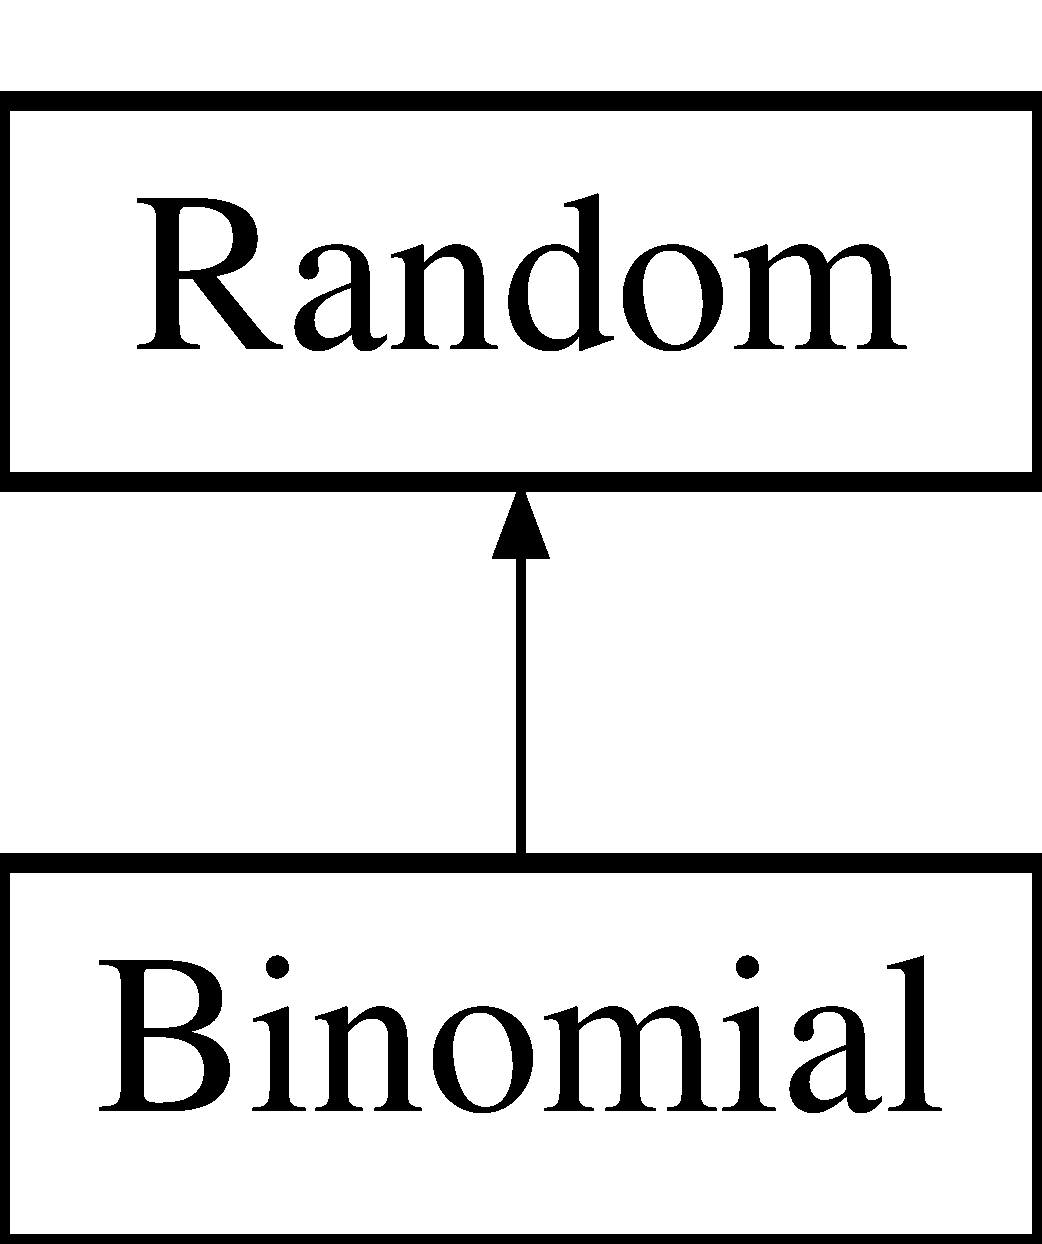
\includegraphics[height=2.000000cm]{classBinomial}
\end{center}
\end{figure}
\subsection*{Public Member Functions}
\begin{DoxyCompactItemize}
\item 
\mbox{\Hypertarget{classBinomial_a428350f0a46f32c41f695e63a46ffa94}\label{classBinomial_a428350f0a46f32c41f695e63a46ffa94}} 
{\bfseries Binomial} (int n, double u, \hyperlink{classRNG}{R\+NG} $\ast$gen)
\item 
\mbox{\Hypertarget{classBinomial_a022822b08181402387ac3a8f4fce35db}\label{classBinomial_a022822b08181402387ac3a8f4fce35db}} 
int {\bfseries n} ()
\item 
\mbox{\Hypertarget{classBinomial_a01acca773a5bdb3e468d78e19a946b24}\label{classBinomial_a01acca773a5bdb3e468d78e19a946b24}} 
int {\bfseries n} (int xn)
\item 
\mbox{\Hypertarget{classBinomial_aa43457c0e0e177c619894425bbcb9879}\label{classBinomial_aa43457c0e0e177c619894425bbcb9879}} 
double {\bfseries u} ()
\item 
\mbox{\Hypertarget{classBinomial_a4fadb644ba8ddae03657401da11b5e81}\label{classBinomial_a4fadb644ba8ddae03657401da11b5e81}} 
double {\bfseries u} (double xu)
\item 
\mbox{\Hypertarget{classBinomial_afa2e867ce22cf0b78b624de7a8f44291}\label{classBinomial_afa2e867ce22cf0b78b624de7a8f44291}} 
virtual double {\bfseries operator()} ()
\end{DoxyCompactItemize}
\subsection*{Protected Attributes}
\begin{DoxyCompactItemize}
\item 
\mbox{\Hypertarget{classBinomial_a7b043cf18cd7a22f4bbadd5a94932c8f}\label{classBinomial_a7b043cf18cd7a22f4bbadd5a94932c8f}} 
int {\bfseries pN}
\item 
\mbox{\Hypertarget{classBinomial_ae4dd874e53dde7f2041e13a1bf356447}\label{classBinomial_ae4dd874e53dde7f2041e13a1bf356447}} 
double {\bfseries pU}
\end{DoxyCompactItemize}


The documentation for this class was generated from the following files\+:\begin{DoxyCompactItemize}
\item 
/home/fallon/git/merlin-\/cmake/\+Merlin/Binomial.\+h\item 
/home/fallon/git/merlin-\/cmake/\+Merlin/Binomial.\+cpp\end{DoxyCompactItemize}

\hypertarget{classBPM}{}\section{B\+PM Class Reference}
\label{classBPM}\index{B\+PM@{B\+PM}}
Inheritance diagram for B\+PM\+:\begin{figure}[H]
\begin{center}
\leavevmode
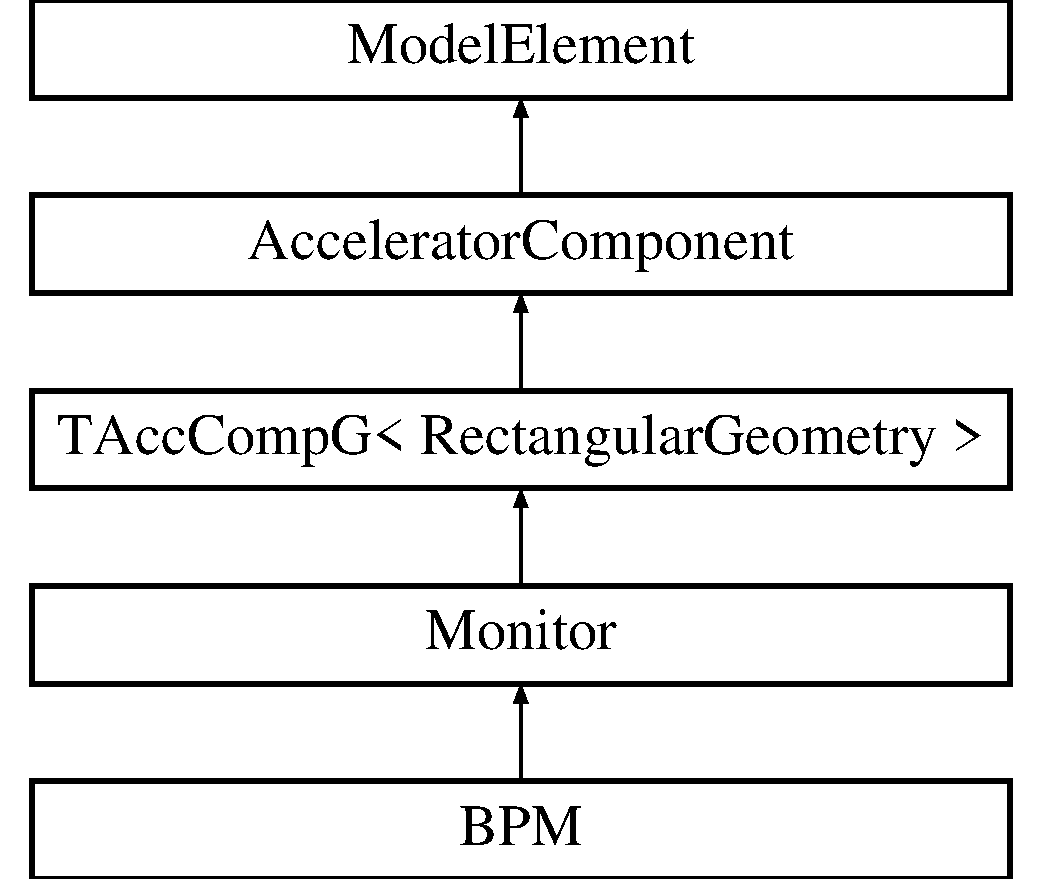
\includegraphics[height=5.000000cm]{classBPM}
\end{center}
\end{figure}
\subsection*{Classes}
\begin{DoxyCompactItemize}
\item 
class \hyperlink{classBPM_1_1Buffer}{Buffer}
\item 
struct \hyperlink{structBPM_1_1Data}{Data}
\item 
class \hyperlink{classBPM_1_1Response}{Response}
\end{DoxyCompactItemize}
\subsection*{Public Types}
\begin{DoxyCompactItemize}
\item 
\mbox{\Hypertarget{classBPM_a191c31480c5ccefd8ce44c84ca19ebcf}\label{classBPM_a191c31480c5ccefd8ce44c84ca19ebcf}} 
typedef \hyperlink{classAMBufferManager}{A\+M\+Buffer\+Manager}$<$ \hyperlink{classBPM}{B\+PM}, \hyperlink{classBPM_1_1Buffer}{Buffer}, \hyperlink{structBPM_1_1Data}{Data} $>$ {\bfseries Buffer\+Manager}
\end{DoxyCompactItemize}
\subsection*{Public Member Functions}
\begin{DoxyCompactItemize}
\item 
\mbox{\Hypertarget{classBPM_a5b3c7aea940a5894dfcaca0a3e3ca999}\label{classBPM_a5b3c7aea940a5894dfcaca0a3e3ca999}} 
{\bfseries B\+PM} (const string \&\hyperlink{classModelElement_aada171ead2085c75b592cf07d91bc5c2}{id}, double len=0, double mpos=0)
\item 
\mbox{\Hypertarget{classBPM_a3d13a6666a7ed0764c032ccc6cc326bf}\label{classBPM_a3d13a6666a7ed0764c032ccc6cc326bf}} 
void {\bfseries Set\+Resolution} (double xr, double yr)
\item 
\mbox{\Hypertarget{classBPM_aa13a91f52e78d6610b16b21639deb390}\label{classBPM_aa13a91f52e78d6610b16b21639deb390}} 
double {\bfseries Set\+Res} (double r)
\item 
\mbox{\Hypertarget{classBPM_ab6e698f9655b8b13bed9f7dc7f70cf1e}\label{classBPM_ab6e698f9655b8b13bed9f7dc7f70cf1e}} 
void {\bfseries Set\+Scale} (double xs, double ys)
\item 
\mbox{\Hypertarget{classBPM_aa34bd41aa62234b3a956b6dad58d739c}\label{classBPM_aa34bd41aa62234b3a956b6dad58d739c}} 
\hyperlink{classBPM_1_1Response}{Response} $\ast$ {\bfseries Set\+Response} (\hyperlink{classBPM_1_1Response}{Response} $\ast$)
\item 
\mbox{\Hypertarget{classBPM_a5fc14b1e25177f95ef65dba3becc2663}\label{classBPM_a5fc14b1e25177f95ef65dba3becc2663}} 
virtual void {\bfseries Make\+Measurement} (const \hyperlink{classBunch}{Bunch} \&a\+Bunch)
\item 
virtual int \hyperlink{classBPM_acaf99f021f92252962f2fbcbc24a2679}{Get\+Index} () const
\item 
virtual const string \& \hyperlink{classBPM_a1fbab5ffd976674ed24ef5833caaf7ee}{Get\+Type} () const
\item 
virtual void \hyperlink{classBPM_a3f0db54eff4f4e95fc2dd81728ea8759}{Prepare\+Tracker} (\hyperlink{classComponentTracker}{Component\+Tracker} \&a\+Tracker)
\item 
virtual \hyperlink{classModelElement}{Model\+Element} $\ast$ \hyperlink{classBPM_a21bba21422046a434a38268c0cb5ada6}{Copy} () const
\item 
\mbox{\Hypertarget{classBPM_ac1116db96cd45fdc5916c051e55ea454}\label{classBPM_ac1116db96cd45fdc5916c051e55ea454}} 
void {\bfseries Add\+Buffer} (\hyperlink{classBPM_1_1Buffer}{Buffer} $\ast$abuffer)
\item 
\mbox{\Hypertarget{classBPM_aa34dbcecc2c8febed932371753e903b6}\label{classBPM_aa34dbcecc2c8febed932371753e903b6}} 
bool {\bfseries Remove\+Buffer} (\hyperlink{classBPM_1_1Buffer}{Buffer} $\ast$a\+Buffer)
\item 
\mbox{\Hypertarget{classBPM_a1c2f74ef9b72e81da05fc682ae04e03d}\label{classBPM_a1c2f74ef9b72e81da05fc682ae04e03d}} 
void {\bfseries Clear\+All\+Buffers} ()
\end{DoxyCompactItemize}
\subsection*{Static Public Member Functions}
\begin{DoxyCompactItemize}
\item 
\mbox{\Hypertarget{classBPM_a11a2523361aa03be19252b5335efdc48}\label{classBPM_a11a2523361aa03be19252b5335efdc48}} 
static void {\bfseries Set\+Default\+Buffer} (\hyperlink{classBPM_1_1Buffer}{Buffer} $\ast$buffer)
\end{DoxyCompactItemize}
\subsection*{Static Public Attributes}
\begin{DoxyCompactItemize}
\item 
\mbox{\Hypertarget{classBPM_a093ea71219d65492338ac96da3df0b70}\label{classBPM_a093ea71219d65492338ac96da3df0b70}} 
static const int {\bfseries ID} = \hyperlink{classAcceleratorComponent_aa7ad4d39e1a488b705983842ed1ac784}{Unique\+Index}()
\item 
\mbox{\Hypertarget{classBPM_acdece9060883eb54d96949f62ae5e91c}\label{classBPM_acdece9060883eb54d96949f62ae5e91c}} 
static bool {\bfseries generate\+\_\+noise} = true
\end{DoxyCompactItemize}
\subsection*{Additional Inherited Members}


\subsection{Member Function Documentation}
\mbox{\Hypertarget{classBPM_a21bba21422046a434a38268c0cb5ada6}\label{classBPM_a21bba21422046a434a38268c0cb5ada6}} 
\index{B\+PM@{B\+PM}!Copy@{Copy}}
\index{Copy@{Copy}!B\+PM@{B\+PM}}
\subsubsection{\texorpdfstring{Copy()}{Copy()}}
{\footnotesize\ttfamily \hyperlink{classModelElement}{Model\+Element} $\ast$ B\+P\+M\+::\+Copy (\begin{DoxyParamCaption}{ }\end{DoxyParamCaption}) const\hspace{0.3cm}{\ttfamily [virtual]}}

Virtual constructor. 

Reimplemented from \hyperlink{classMonitor_a66d7932308a7206eeefc552bd3f5b1f6}{Monitor}.

\mbox{\Hypertarget{classBPM_acaf99f021f92252962f2fbcbc24a2679}\label{classBPM_acaf99f021f92252962f2fbcbc24a2679}} 
\index{B\+PM@{B\+PM}!Get\+Index@{Get\+Index}}
\index{Get\+Index@{Get\+Index}!B\+PM@{B\+PM}}
\subsubsection{\texorpdfstring{Get\+Index()}{GetIndex()}}
{\footnotesize\ttfamily int B\+P\+M\+::\+Get\+Index (\begin{DoxyParamCaption}{ }\end{DoxyParamCaption}) const\hspace{0.3cm}{\ttfamily [virtual]}}

Returns the unique index for this class of accelerator components. \begin{DoxyReturn}{Returns}
An integer containing the unique index for this \hyperlink{classAcceleratorComponent}{Accelerator\+Component} type. 
\end{DoxyReturn}


Reimplemented from \hyperlink{classMonitor_a38297eb50d06dd56201f2b48d92aa789}{Monitor}.

\mbox{\Hypertarget{classBPM_a1fbab5ffd976674ed24ef5833caaf7ee}\label{classBPM_a1fbab5ffd976674ed24ef5833caaf7ee}} 
\index{B\+PM@{B\+PM}!Get\+Type@{Get\+Type}}
\index{Get\+Type@{Get\+Type}!B\+PM@{B\+PM}}
\subsubsection{\texorpdfstring{Get\+Type()}{GetType()}}
{\footnotesize\ttfamily const string \& B\+P\+M\+::\+Get\+Type (\begin{DoxyParamCaption}{ }\end{DoxyParamCaption}) const\hspace{0.3cm}{\ttfamily [virtual]}}

Return the type string for the element. \begin{DoxyReturn}{Returns}
A string containing the type of the element. 
\end{DoxyReturn}


Reimplemented from \hyperlink{classMonitor_a8408f173bef0f0c0dd89b6624c84f66b}{Monitor}.

\mbox{\Hypertarget{classBPM_a3f0db54eff4f4e95fc2dd81728ea8759}\label{classBPM_a3f0db54eff4f4e95fc2dd81728ea8759}} 
\index{B\+PM@{B\+PM}!Prepare\+Tracker@{Prepare\+Tracker}}
\index{Prepare\+Tracker@{Prepare\+Tracker}!B\+PM@{B\+PM}}
\subsubsection{\texorpdfstring{Prepare\+Tracker()}{PrepareTracker()}}
{\footnotesize\ttfamily void B\+P\+M\+::\+Prepare\+Tracker (\begin{DoxyParamCaption}\item[{\hyperlink{classComponentTracker}{Component\+Tracker} \&}]{a\+Tracker }\end{DoxyParamCaption})\hspace{0.3cm}{\ttfamily [virtual]}}

Primary tracking interface. Prepares the specified Tracker object for tracking this component. 
\begin{DoxyParams}[1]{Parameters}
\mbox{\tt in,out}  & {\em a\+Tracker} & The tracker to prepare. \\
\hline
\end{DoxyParams}


Reimplemented from \hyperlink{classMonitor_a8d5e3ab0d68f89a51aabdcde2b01977a}{Monitor}.



The documentation for this class was generated from the following files\+:\begin{DoxyCompactItemize}
\item 
/home/fallon/git/merlin-\/cmake/\+Merlin/B\+P\+M.\+h\item 
/home/fallon/git/merlin-\/cmake/\+Merlin/B\+P\+M.\+cpp\end{DoxyCompactItemize}

\hypertarget{classBPMChannel}{}\section{B\+P\+M\+Channel Class Reference}
\label{classBPMChannel}\index{B\+P\+M\+Channel@{B\+P\+M\+Channel}}
Inheritance diagram for B\+P\+M\+Channel\+:\begin{figure}[H]
\begin{center}
\leavevmode
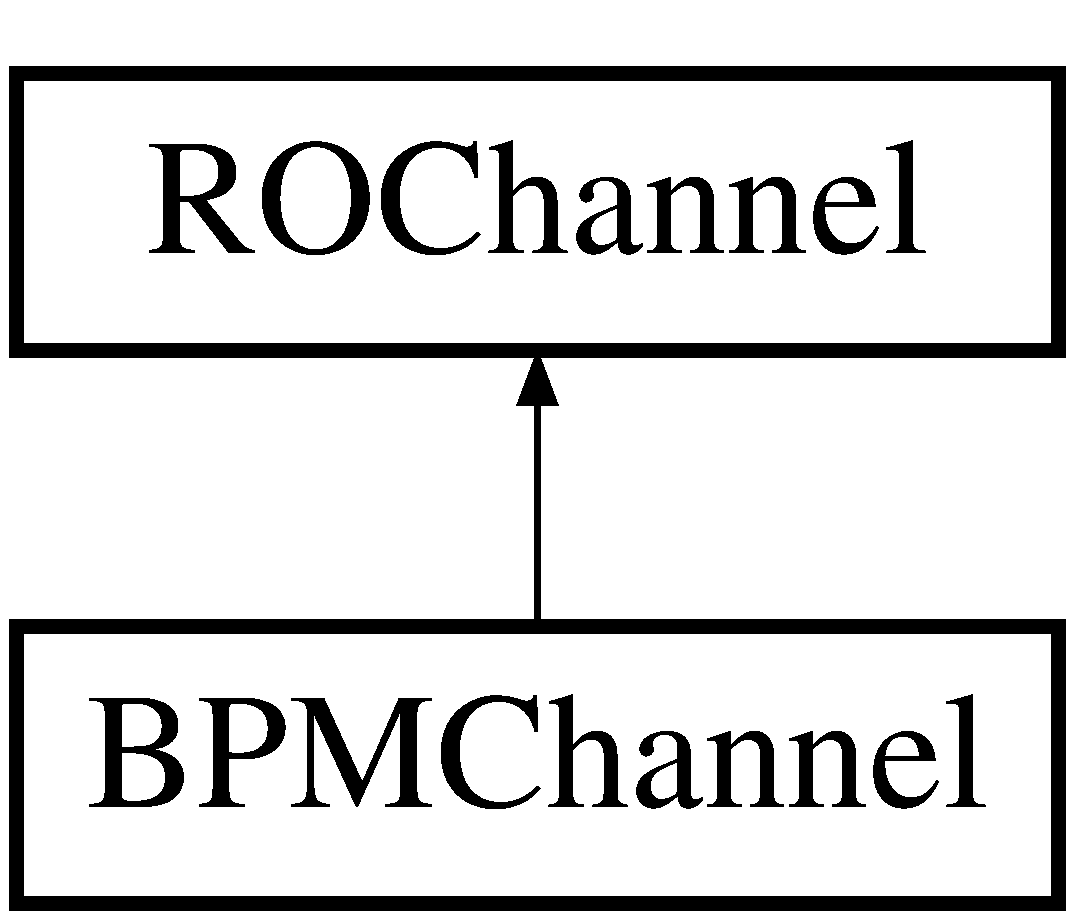
\includegraphics[height=2.000000cm]{classBPMChannel}
\end{center}
\end{figure}
\subsection*{Public Member Functions}
\begin{DoxyCompactItemize}
\item 
\mbox{\Hypertarget{classBPMChannel_aa12b2a5d9774cd741c45d79596bf9f4b}\label{classBPMChannel_aa12b2a5d9774cd741c45d79596bf9f4b}} 
{\bfseries B\+P\+M\+Channel} (char XorY, \hyperlink{classBPMDataBuffer}{B\+P\+M\+Data\+Buffer} $\ast$data\+Buff)
\item 
\mbox{\Hypertarget{classBPMChannel_a460efd551918caf02c04914da18c6d57}\label{classBPMChannel_a460efd551918caf02c04914da18c6d57}} 
virtual std\+::string {\bfseries Get\+ID} () const
\item 
\mbox{\Hypertarget{classBPMChannel_a31e679f16b475899d5f45a10363cb0a0}\label{classBPMChannel_a31e679f16b475899d5f45a10363cb0a0}} 
virtual double {\bfseries Read} () const
\item 
\mbox{\Hypertarget{classBPMChannel_aae9880f3570c3833bc5d43f75d5dc529}\label{classBPMChannel_aae9880f3570c3833bc5d43f75d5dc529}} 
void {\bfseries Set\+B\+P\+M\+Offset} (double v)
\end{DoxyCompactItemize}


The documentation for this class was generated from the following files\+:\begin{DoxyCompactItemize}
\item 
/home/fallon/git/merlin-\/cmake/\+Merlin/B\+P\+M\+Channel.\+h\item 
/home/fallon/git/merlin-\/cmake/\+Merlin/B\+P\+M\+Channel.\+cpp\end{DoxyCompactItemize}

\hypertarget{classBPMChannelCtor}{}\section{B\+P\+M\+Channel\+Ctor Class Reference}
\label{classBPMChannelCtor}\index{B\+P\+M\+Channel\+Ctor@{B\+P\+M\+Channel\+Ctor}}
Inheritance diagram for B\+P\+M\+Channel\+Ctor\+:\begin{figure}[H]
\begin{center}
\leavevmode
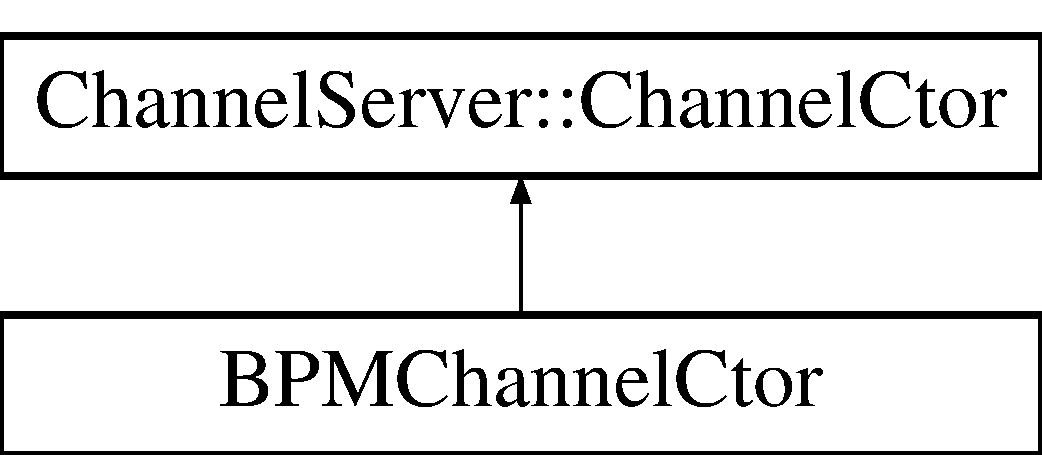
\includegraphics[height=2.000000cm]{classBPMChannelCtor}
\end{center}
\end{figure}
\subsection*{Public Member Functions}
\begin{DoxyCompactItemize}
\item 
\mbox{\Hypertarget{classBPMChannelCtor_a04a47491e8aaa4bbc6b737cacd72d1a3}\label{classBPMChannelCtor_a04a47491e8aaa4bbc6b737cacd72d1a3}} 
{\bfseries B\+P\+M\+Channel\+Ctor} (char xy)
\item 
\mbox{\Hypertarget{classBPMChannelCtor_a6679bced189b1099cffcd04e624b0702}\label{classBPMChannelCtor_a6679bced189b1099cffcd04e624b0702}} 
virtual \hyperlink{classROChannel}{R\+O\+Channel} $\ast$ {\bfseries Construct\+RO} (\hyperlink{classModelElement}{Model\+Element} $\ast$an\+Element)
\item 
\mbox{\Hypertarget{classBPMChannelCtor_ac25de30b6e0bee8cfd2152d9c03e8d4d}\label{classBPMChannelCtor_ac25de30b6e0bee8cfd2152d9c03e8d4d}} 
virtual \hyperlink{classRWChannel}{R\+W\+Channel} $\ast$ {\bfseries Construct\+RW} (\hyperlink{classModelElement}{Model\+Element} $\ast$an\+Element)
\end{DoxyCompactItemize}
\subsection*{Static Public Attributes}
\begin{DoxyCompactItemize}
\item 
\mbox{\Hypertarget{classBPMChannelCtor_a18f9bbeb19f981ae0c342efd0c4ad5bf}\label{classBPMChannelCtor_a18f9bbeb19f981ae0c342efd0c4ad5bf}} 
static \hyperlink{classBPMDataBufferServer}{B\+P\+M\+Data\+Buffer\+Server} {\bfseries the\+Server}
\end{DoxyCompactItemize}
\subsection*{Additional Inherited Members}


The documentation for this class was generated from the following files\+:\begin{DoxyCompactItemize}
\item 
/home/fallon/git/merlin-\/cmake/\+Merlin/B\+P\+M\+Channel\+Ctor.\+h\item 
/home/fallon/git/merlin-\/cmake/\+Merlin/B\+P\+M\+Channel\+Ctor.\+cpp\end{DoxyCompactItemize}

\hypertarget{classBPMDataBuffer}{}\section{B\+P\+M\+Data\+Buffer Class Reference}
\label{classBPMDataBuffer}\index{B\+P\+M\+Data\+Buffer@{B\+P\+M\+Data\+Buffer}}
Inheritance diagram for B\+P\+M\+Data\+Buffer\+:\begin{figure}[H]
\begin{center}
\leavevmode
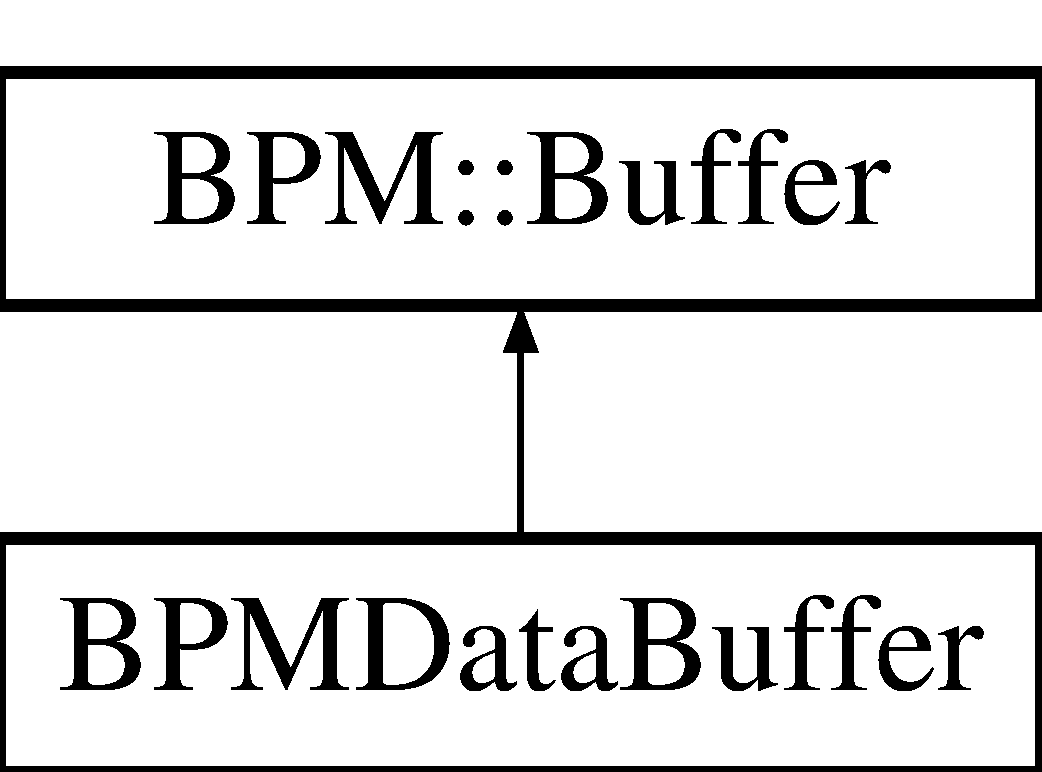
\includegraphics[height=2.000000cm]{classBPMDataBuffer}
\end{center}
\end{figure}
\subsection*{Public Member Functions}
\begin{DoxyCompactItemize}
\item 
\mbox{\Hypertarget{classBPMDataBuffer_a8710bff1ff2db1bc54d93f92d8ceb7bf}\label{classBPMDataBuffer_a8710bff1ff2db1bc54d93f92d8ceb7bf}} 
virtual void {\bfseries Record} (const \hyperlink{classBPM}{B\+PM} \&a\+B\+PM, const \hyperlink{structBPM_1_1Data}{B\+P\+M\+::\+Data} \&data)
\item 
\mbox{\Hypertarget{classBPMDataBuffer_af220d26561b1e99b443bde1131702066}\label{classBPMDataBuffer_af220d26561b1e99b443bde1131702066}} 
void {\bfseries Set\+ID} (const string \&an\+ID)
\item 
\mbox{\Hypertarget{classBPMDataBuffer_ab0767c41e8d3eae8277fdc6b193269d0}\label{classBPMDataBuffer_ab0767c41e8d3eae8277fdc6b193269d0}} 
void {\bfseries Set\+Offsets} (double x, double y)
\end{DoxyCompactItemize}
\subsection*{Friends}
\begin{DoxyCompactItemize}
\item 
\mbox{\Hypertarget{classBPMDataBuffer_a7d383da5b53613d4683641b8bd04620c}\label{classBPMDataBuffer_a7d383da5b53613d4683641b8bd04620c}} 
class {\bfseries B\+P\+M\+Channel}
\end{DoxyCompactItemize}


The documentation for this class was generated from the following files\+:\begin{DoxyCompactItemize}
\item 
/home/fallon/git/merlin-\/cmake/\+Merlin/B\+P\+M\+Data\+Buffer.\+h\item 
/home/fallon/git/merlin-\/cmake/\+Merlin/B\+P\+M\+Data\+Buffer.\+cpp\end{DoxyCompactItemize}

\hypertarget{classBPMDataBufferServer}{}\section{B\+P\+M\+Data\+Buffer\+Server Class Reference}
\label{classBPMDataBufferServer}\index{B\+P\+M\+Data\+Buffer\+Server@{B\+P\+M\+Data\+Buffer\+Server}}
\subsection*{Public Member Functions}
\begin{DoxyCompactItemize}
\item 
\mbox{\Hypertarget{classBPMDataBufferServer_abf194b7ad1b0ebea5d160b8dce57af5a}\label{classBPMDataBufferServer_abf194b7ad1b0ebea5d160b8dce57af5a}} 
\hyperlink{classBPMDataBuffer}{B\+P\+M\+Data\+Buffer} $\ast$ {\bfseries Get\+Data\+Buffer} (\hyperlink{classBPM}{B\+PM} $\ast$bpm, bool create=true)
\item 
\mbox{\Hypertarget{classBPMDataBufferServer_aeb249391dcc08b5dd055ce48e221afd8}\label{classBPMDataBufferServer_aeb249391dcc08b5dd055ce48e221afd8}} 
void {\bfseries Dump} (ostream \&os)
\end{DoxyCompactItemize}


The documentation for this class was generated from the following files\+:\begin{DoxyCompactItemize}
\item 
/home/fallon/git/merlin-\/cmake/\+Merlin/B\+P\+M\+Data\+Buffer\+Server.\+h\item 
/home/fallon/git/merlin-\/cmake/\+Merlin/B\+P\+M\+Data\+Buffer\+Server.\+cpp\end{DoxyCompactItemize}

\hypertarget{classBPM_1_1Buffer}{}\section{B\+PM\+:\+:Buffer Class Reference}
\label{classBPM_1_1Buffer}\index{B\+P\+M\+::\+Buffer@{B\+P\+M\+::\+Buffer}}
Inheritance diagram for B\+PM\+:\+:Buffer\+:\begin{figure}[H]
\begin{center}
\leavevmode
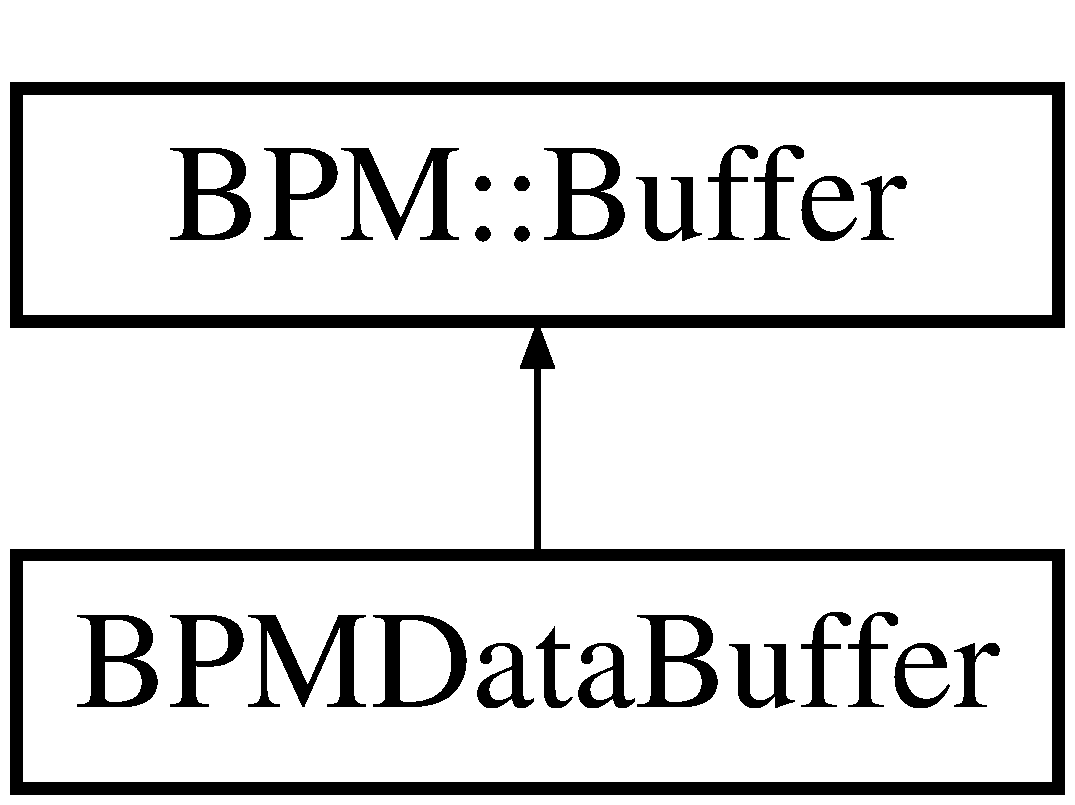
\includegraphics[height=2.000000cm]{classBPM_1_1Buffer}
\end{center}
\end{figure}
\subsection*{Public Member Functions}
\begin{DoxyCompactItemize}
\item 
\mbox{\Hypertarget{classBPM_1_1Buffer_a5e2ffba153542517e30ece29f1927168}\label{classBPM_1_1Buffer_a5e2ffba153542517e30ece29f1927168}} 
virtual void {\bfseries Record} (const \hyperlink{classBPM}{B\+PM} \&a\+B\+PM, const \hyperlink{structBPM_1_1Data}{Data} \&data)=0
\end{DoxyCompactItemize}


The documentation for this class was generated from the following file\+:\begin{DoxyCompactItemize}
\item 
/home/fallon/git/merlin-\/cmake/\+Merlin/B\+P\+M.\+h\end{DoxyCompactItemize}

\hypertarget{classRMSProfileMonitor_1_1Buffer}{}\section{R\+M\+S\+Profile\+Monitor\+:\+:Buffer Class Reference}
\label{classRMSProfileMonitor_1_1Buffer}\index{R\+M\+S\+Profile\+Monitor\+::\+Buffer@{R\+M\+S\+Profile\+Monitor\+::\+Buffer}}
\subsection*{Public Member Functions}
\begin{DoxyCompactItemize}
\item 
\mbox{\Hypertarget{classRMSProfileMonitor_1_1Buffer_ae5da389cea296ad7a2919f2e7b4c90a5}\label{classRMSProfileMonitor_1_1Buffer_ae5da389cea296ad7a2919f2e7b4c90a5}} 
virtual void {\bfseries Record} (const \hyperlink{classRMSProfileMonitor}{R\+M\+S\+Profile\+Monitor} \&mon, const \hyperlink{structRMSProfileMonitor_1_1Data}{Data} \&dat)=0
\end{DoxyCompactItemize}


The documentation for this class was generated from the following file\+:\begin{DoxyCompactItemize}
\item 
/home/fallon/git/merlin-\/cmake/\+Merlin/R\+M\+S\+Profile\+Monitor.\+h\end{DoxyCompactItemize}

\hypertarget{classBunch}{}\section{Bunch Class Reference}
\label{classBunch}\index{Bunch@{Bunch}}
Inheritance diagram for Bunch\+:\begin{figure}[H]
\begin{center}
\leavevmode
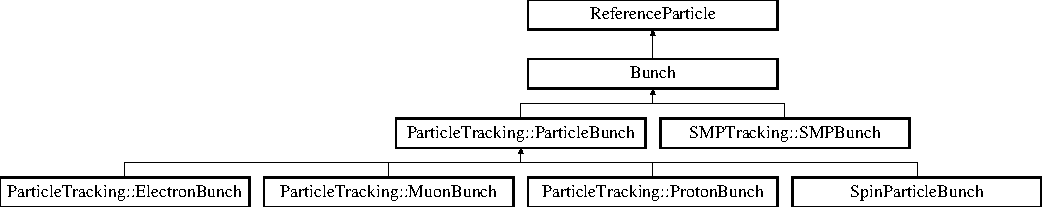
\includegraphics[height=2.786070cm]{classBunch}
\end{center}
\end{figure}
\subsection*{Public Member Functions}
\begin{DoxyCompactItemize}
\item 
\mbox{\Hypertarget{classBunch_a8bfec1887f57505cafcad9a0acf6d3ca}\label{classBunch_a8bfec1887f57505cafcad9a0acf6d3ca}} 
{\bfseries Bunch} (double p, double q)
\item 
\mbox{\Hypertarget{classBunch_a946942aa6a7404ce13b5103abc7a3dfe}\label{classBunch_a946942aa6a7404ce13b5103abc7a3dfe}} 
virtual double {\bfseries Get\+Total\+Charge} () const =0
\item 
\mbox{\Hypertarget{classBunch_a204ba650bb0ff67d7fd75477da70766f}\label{classBunch_a204ba650bb0ff67d7fd75477da70766f}} 
virtual \hyperlink{classTPSMoments}{P\+Smoments} \& {\bfseries Get\+Moments} (\hyperlink{classTPSMoments}{P\+Smoments} \&sigma) const =0
\item 
\mbox{\Hypertarget{classBunch_a9262fb601fe43bffc9cb2debd5ffdb73}\label{classBunch_a9262fb601fe43bffc9cb2debd5ffdb73}} 
\hyperlink{classTPSMoments}{P\+Smoments} {\bfseries Get\+Moments} () const
\item 
\mbox{\Hypertarget{classBunch_a77d7e164f04dd31d73f7f1014fb8feec}\label{classBunch_a77d7e164f04dd31d73f7f1014fb8feec}} 
virtual \hyperlink{classTPSMoments_3_011_01_4}{P\+Smoments2D} \& {\bfseries Get\+Projected\+Moments} (P\+Scoord u, P\+Scoord v, \hyperlink{classTPSMoments_3_011_01_4}{P\+Smoments2D} \&sigma) const =0
\item 
\mbox{\Hypertarget{classBunch_a0259dd62c200a2f6df6595cb352bebca}\label{classBunch_a0259dd62c200a2f6df6595cb352bebca}} 
virtual \hyperlink{classPSvector}{P\+Svector} \& {\bfseries Get\+Centroid} (\hyperlink{classPSvector}{P\+Svector} \&p) const =0
\item 
\mbox{\Hypertarget{classBunch_a5ccc9ef2f9ff77b09bd7b4a636975455}\label{classBunch_a5ccc9ef2f9ff77b09bd7b4a636975455}} 
virtual \hyperlink{classTVec2D}{Point2D} {\bfseries Get\+Projected\+Centroid} (P\+Scoord u, P\+Scoord v) const =0
\item 
\mbox{\Hypertarget{classBunch_a37ff416d2fab31ab4db21e10662529d8}\label{classBunch_a37ff416d2fab31ab4db21e10662529d8}} 
virtual double {\bfseries Adjust\+Ref\+Momentum\+To\+Mean} ()=0
\item 
\mbox{\Hypertarget{classBunch_a350e2213fc71673b56ad3570aaa7674a}\label{classBunch_a350e2213fc71673b56ad3570aaa7674a}} 
virtual double {\bfseries Adjust\+Ref\+Time\+To\+Mean} ()=0
\item 
\mbox{\Hypertarget{classBunch_a6d87afade5729dcb2830a8c3fc3ee862}\label{classBunch_a6d87afade5729dcb2830a8c3fc3ee862}} 
virtual void {\bfseries Output} (std\+::ostream \&os) const =0
\item 
\mbox{\Hypertarget{classBunch_acb5f121fce6c8334f37e79db78348c2a}\label{classBunch_acb5f121fce6c8334f37e79db78348c2a}} 
virtual Histogram \& {\bfseries Project\+Distribution} (P\+Scoord axis, Histogram \&hist) const =0
\item 
\mbox{\Hypertarget{classBunch_af67bae6bc37a75e9a5ead6093b6eda96}\label{classBunch_af67bae6bc37a75e9a5ead6093b6eda96}} 
virtual bool {\bfseries Apply\+Transformation} (const \hyperlink{classTransform3D}{Transform3D} \&t)=0
\end{DoxyCompactItemize}
\subsection*{Additional Inherited Members}


The documentation for this class was generated from the following file\+:\begin{DoxyCompactItemize}
\item 
/home/fallon/git/merlin-\/cmake/\+Merlin/Bunch.\+h\end{DoxyCompactItemize}

\hypertarget{classBunchConstructor}{}\section{Bunch\+Constructor Class Reference}
\label{classBunchConstructor}\index{Bunch\+Constructor@{Bunch\+Constructor}}
Inheritance diagram for Bunch\+Constructor\+:\begin{figure}[H]
\begin{center}
\leavevmode
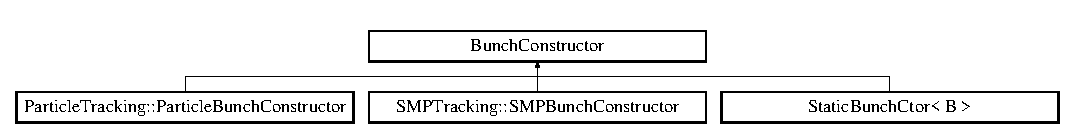
\includegraphics[height=1.419518cm]{classBunchConstructor}
\end{center}
\end{figure}
\subsection*{Public Member Functions}
\begin{DoxyCompactItemize}
\item 
\mbox{\Hypertarget{classBunchConstructor_ace0adecca72de2979692b2c1deb79674}\label{classBunchConstructor_ace0adecca72de2979692b2c1deb79674}} 
virtual \hyperlink{classBunch}{Bunch} $\ast$ {\bfseries Construct\+Bunch} (int bunch\+Index=0) const =0
\end{DoxyCompactItemize}


The documentation for this class was generated from the following file\+:\begin{DoxyCompactItemize}
\item 
/home/fallon/git/merlin-\/cmake/\+Merlin/Bunch\+Constructor.\+h\end{DoxyCompactItemize}

\hypertarget{classBunchProcess}{}\section{Bunch\+Process Class Reference}
\label{classBunchProcess}\index{Bunch\+Process@{Bunch\+Process}}
Inheritance diagram for Bunch\+Process\+:\begin{figure}[H]
\begin{center}
\leavevmode
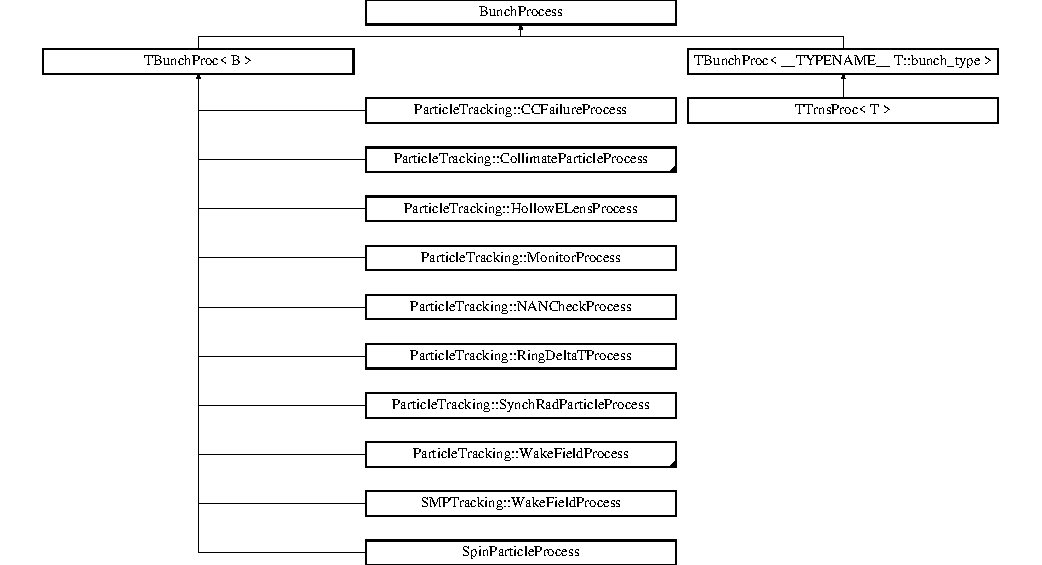
\includegraphics[height=7.593220cm]{classBunchProcess}
\end{center}
\end{figure}
\subsection*{Public Member Functions}
\begin{DoxyCompactItemize}
\item 
\mbox{\Hypertarget{classBunchProcess_a5ec5af6ed253cd2f92dab04a6ee7a301}\label{classBunchProcess_a5ec5af6ed253cd2f92dab04a6ee7a301}} 
{\bfseries Bunch\+Process} (const string \&an\+ID, int a\+Priority=0)
\item 
\mbox{\Hypertarget{classBunchProcess_aa3110b3448fb4c5ce859f6dd0cc5a1eb}\label{classBunchProcess_aa3110b3448fb4c5ce859f6dd0cc5a1eb}} 
void {\bfseries Set\+Priority} (int p)
\item 
\mbox{\Hypertarget{classBunchProcess_a29d3480447a2035719f43b1c95d51a20}\label{classBunchProcess_a29d3480447a2035719f43b1c95d51a20}} 
int {\bfseries Get\+Priority} () const
\item 
\mbox{\Hypertarget{classBunchProcess_a8c8732d2cc71b545387a27cc8adc74ff}\label{classBunchProcess_a8c8732d2cc71b545387a27cc8adc74ff}} 
virtual void {\bfseries Initialise\+Process} (\hyperlink{classBunch}{Bunch} \&bunch)=0
\item 
\mbox{\Hypertarget{classBunchProcess_a319a4b99d3b042832af4f18a733403fd}\label{classBunchProcess_a319a4b99d3b042832af4f18a733403fd}} 
virtual void {\bfseries Set\+Current\+Component} (\hyperlink{classAcceleratorComponent}{Accelerator\+Component} \&component)
\item 
\mbox{\Hypertarget{classBunchProcess_a8add569705fe42dac0dbc1504d774901}\label{classBunchProcess_a8add569705fe42dac0dbc1504d774901}} 
virtual void {\bfseries Do\+Process} (double ds)=0
\item 
\mbox{\Hypertarget{classBunchProcess_a6bfda24adc7b189da4affba9b01b8240}\label{classBunchProcess_a6bfda24adc7b189da4affba9b01b8240}} 
virtual double {\bfseries Get\+Max\+Allowed\+Step\+Size} () const =0
\item 
\mbox{\Hypertarget{classBunchProcess_af6dcbeb4426b78109b73db2d3adcb8e5}\label{classBunchProcess_af6dcbeb4426b78109b73db2d3adcb8e5}} 
bool {\bfseries Is\+Active} () const
\item 
\mbox{\Hypertarget{classBunchProcess_a416caaff14b5ca631fe262baf83ccf1a}\label{classBunchProcess_a416caaff14b5ca631fe262baf83ccf1a}} 
const string \& {\bfseries Get\+ID} () const
\end{DoxyCompactItemize}
\subsection*{Protected Attributes}
\begin{DoxyCompactItemize}
\item 
\mbox{\Hypertarget{classBunchProcess_a1195731a895d235e3bb209a9d68403e2}\label{classBunchProcess_a1195731a895d235e3bb209a9d68403e2}} 
bool {\bfseries active}
\item 
\mbox{\Hypertarget{classBunchProcess_a296359b6cf1acd671709188cee5a39f4}\label{classBunchProcess_a296359b6cf1acd671709188cee5a39f4}} 
\hyperlink{classAcceleratorComponent}{Accelerator\+Component} $\ast$ {\bfseries current\+Component}
\end{DoxyCompactItemize}


The documentation for this class was generated from the following file\+:\begin{DoxyCompactItemize}
\item 
/home/fallon/git/merlin-\/cmake/\+Merlin/Bunch\+Process.\+h\end{DoxyCompactItemize}

\hypertarget{classBunchTracker}{}\section{Bunch\+Tracker$<$ P $>$ Class Template Reference}
\label{classBunchTracker}\index{Bunch\+Tracker$<$ P $>$@{Bunch\+Tracker$<$ P $>$}}


{\ttfamily \#include $<$Tracking\+Simulation.\+h$>$}

Inheritance diagram for Bunch\+Tracker$<$ P $>$\+:\begin{figure}[H]
\begin{center}
\leavevmode
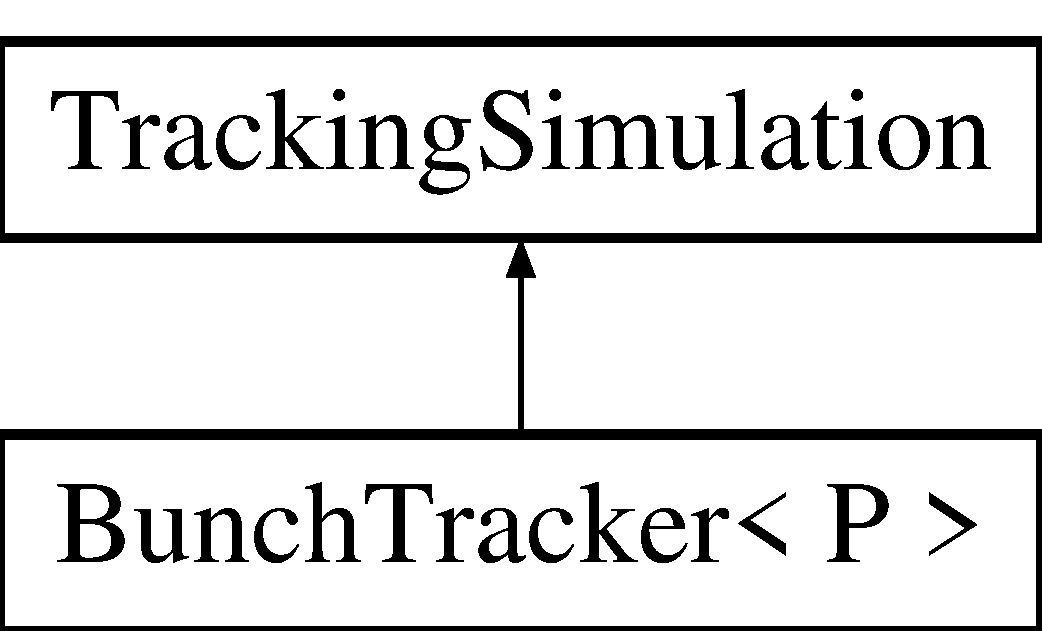
\includegraphics[height=2.000000cm]{classBunchTracker}
\end{center}
\end{figure}
\subsection*{Public Types}
\begin{DoxyCompactItemize}
\item 
\mbox{\Hypertarget{classBunchTracker_a29e2137d8cc489998b6866707b1e326b}\label{classBunchTracker_a29e2137d8cc489998b6866707b1e326b}} 
typedef P\+::bunch\+\_\+type {\bfseries bunch\+\_\+type}
\item 
\mbox{\Hypertarget{classBunchTracker_a169c5a919b7864192d34f96ae5ad0b5e}\label{classBunchTracker_a169c5a919b7864192d34f96ae5ad0b5e}} 
typedef P {\bfseries transport\+\_\+process}
\end{DoxyCompactItemize}
\subsection*{Public Member Functions}
\begin{DoxyCompactItemize}
\item 
\hyperlink{classBunchTracker_a724b0e1b99f6b86e8ba7922461548e18}{Bunch\+Tracker} (const \hyperlink{classAcceleratorModel_1_1Beamline}{Accelerator\+Model\+::\+Beamline} \&bline)
\item 
\hyperlink{classBunchTracker_aac4546a7a80bd46d2e428836202e3bad}{Bunch\+Tracker} (const \hyperlink{classAcceleratorModel_1_1Beamline}{Accelerator\+Model\+::\+Beamline} \&bline, bunch\+\_\+type $\ast$bunch0)
\item 
\mbox{\Hypertarget{classBunchTracker_abe4b943181ba4389901d7f2c608b8a63}\label{classBunchTracker_abe4b943181ba4389901d7f2c608b8a63}} 
bunch\+\_\+type \& {\bfseries Get\+Bunch} ()
\item 
\mbox{\Hypertarget{classBunchTracker_a99324bea77d070cf43028114544a9e61}\label{classBunchTracker_a99324bea77d070cf43028114544a9e61}} 
transport\+\_\+process \& {\bfseries Get\+Transport\+Process} ()
\end{DoxyCompactItemize}
\subsection*{Additional Inherited Members}


\subsection{Detailed Description}
\subsubsection*{template$<$class P$>$\newline
class Bunch\+Tracker$<$ P $>$}

A template class which is used to implement a bunch implementation specific \hyperlink{classTrackingSimulation}{Tracking\+Simulation}. P must be a bunch specific transport process which has only a default constructor. It must also define P\+::bunch\+\_\+type which specifies the type of bunch implementation to be tracked. 

\subsection{Constructor \& Destructor Documentation}
\mbox{\Hypertarget{classBunchTracker_a724b0e1b99f6b86e8ba7922461548e18}\label{classBunchTracker_a724b0e1b99f6b86e8ba7922461548e18}} 
\index{Bunch\+Tracker@{Bunch\+Tracker}!Bunch\+Tracker@{Bunch\+Tracker}}
\index{Bunch\+Tracker@{Bunch\+Tracker}!Bunch\+Tracker@{Bunch\+Tracker}}
\subsubsection{\texorpdfstring{Bunch\+Tracker()}{BunchTracker()}\hspace{0.1cm}{\footnotesize\ttfamily [1/2]}}
{\footnotesize\ttfamily template$<$class P $>$ \\
\hyperlink{classBunchTracker}{Bunch\+Tracker}$<$ P $>$\+::\hyperlink{classBunchTracker}{Bunch\+Tracker} (\begin{DoxyParamCaption}\item[{const \hyperlink{classAcceleratorModel_1_1Beamline}{Accelerator\+Model\+::\+Beamline} \&}]{bline }\end{DoxyParamCaption})\hspace{0.3cm}{\ttfamily [inline]}, {\ttfamily [explicit]}}

Constructor taking the beamline to be tracked. The initial bunch must be specified by supplying a concrete \hyperlink{classBunchConstructor}{Bunch\+Constructor} via Set\+Initial\+Bunch\+Ctor. \mbox{\Hypertarget{classBunchTracker_aac4546a7a80bd46d2e428836202e3bad}\label{classBunchTracker_aac4546a7a80bd46d2e428836202e3bad}} 
\index{Bunch\+Tracker@{Bunch\+Tracker}!Bunch\+Tracker@{Bunch\+Tracker}}
\index{Bunch\+Tracker@{Bunch\+Tracker}!Bunch\+Tracker@{Bunch\+Tracker}}
\subsubsection{\texorpdfstring{Bunch\+Tracker()}{BunchTracker()}\hspace{0.1cm}{\footnotesize\ttfamily [2/2]}}
{\footnotesize\ttfamily template$<$class P $>$ \\
\hyperlink{classBunchTracker}{Bunch\+Tracker}$<$ P $>$\+::\hyperlink{classBunchTracker}{Bunch\+Tracker} (\begin{DoxyParamCaption}\item[{const \hyperlink{classAcceleratorModel_1_1Beamline}{Accelerator\+Model\+::\+Beamline} \&}]{bline,  }\item[{bunch\+\_\+type $\ast$}]{bunch0 }\end{DoxyParamCaption})\hspace{0.3cm}{\ttfamily [inline]}}

Constructs a \hyperlink{classBunchTracker}{Bunch\+Tracker} taking the beamline to be tracked and the initial bunch to be used. 

The documentation for this class was generated from the following file\+:\begin{DoxyCompactItemize}
\item 
/home/fallon/git/merlin-\/cmake/\+Merlin/Tracking\+Simulation.\+h\end{DoxyCompactItemize}

\hypertarget{classBzField}{}\section{Bz\+Field Class Reference}
\label{classBzField}\index{Bz\+Field@{Bz\+Field}}
Inheritance diagram for Bz\+Field\+:\begin{figure}[H]
\begin{center}
\leavevmode
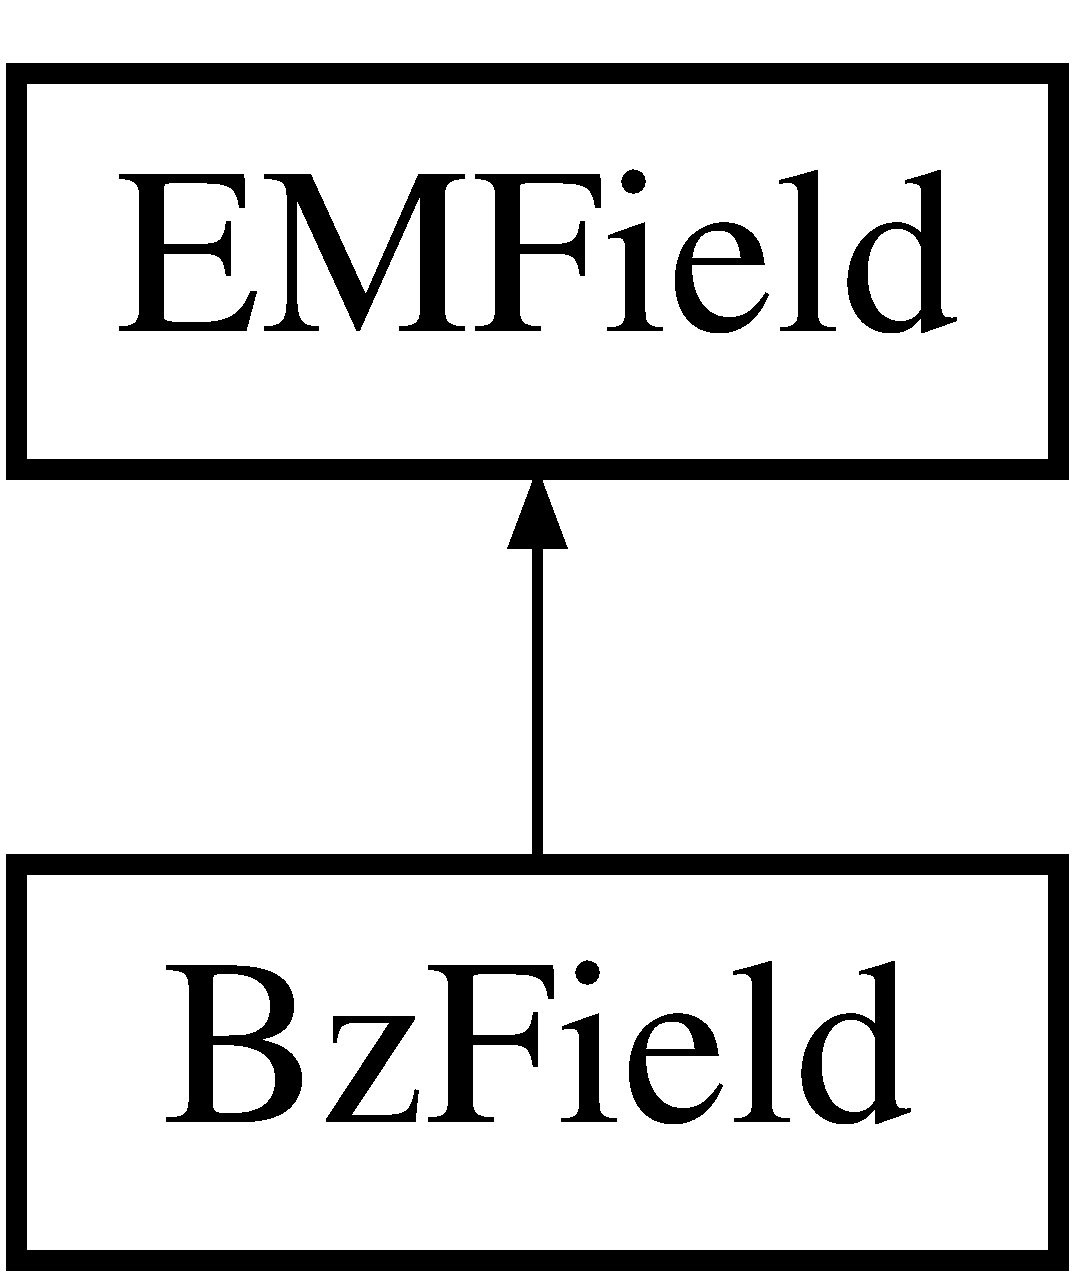
\includegraphics[height=2.000000cm]{classBzField}
\end{center}
\end{figure}
\subsection*{Public Member Functions}
\begin{DoxyCompactItemize}
\item 
\mbox{\Hypertarget{classBzField_a0d34ffdce32cfd2323417a73082de638}\label{classBzField_a0d34ffdce32cfd2323417a73082de638}} 
{\bfseries Bz\+Field} (double B)
\item 
\mbox{\Hypertarget{classBzField_a5469af2716fcda0e6111410413fe5cde}\label{classBzField_a5469af2716fcda0e6111410413fe5cde}} 
double {\bfseries Get\+Strength} () const
\item 
virtual \hyperlink{classTVec3D}{Vector3D} \hyperlink{classBzField_a9903383be440aa99b504f5585ddd65f9}{Get\+B\+Field\+At} (const \hyperlink{classTVec3D}{Point3D} \&x, double t=0) const
\item 
virtual \hyperlink{classTVec3D}{Vector3D} \hyperlink{classBzField_a05df21f7fec6b866936b6c8c70883bf0}{Get\+E\+Field\+At} (const \hyperlink{classTVec3D}{Point3D} \&x, double t=0) const
\item 
\mbox{\Hypertarget{classBzField_a585e0732eb58207e6d1e6f0d1c680921}\label{classBzField_a585e0732eb58207e6d1e6f0d1c680921}} 
void {\bfseries Set\+Strength} (double B)
\end{DoxyCompactItemize}


\subsection{Member Function Documentation}
\mbox{\Hypertarget{classBzField_a9903383be440aa99b504f5585ddd65f9}\label{classBzField_a9903383be440aa99b504f5585ddd65f9}} 
\index{Bz\+Field@{Bz\+Field}!Get\+B\+Field\+At@{Get\+B\+Field\+At}}
\index{Get\+B\+Field\+At@{Get\+B\+Field\+At}!Bz\+Field@{Bz\+Field}}
\subsubsection{\texorpdfstring{Get\+B\+Field\+At()}{GetBFieldAt()}}
{\footnotesize\ttfamily \hyperlink{classTVec3D}{Vector3D} Bz\+Field\+::\+Get\+B\+Field\+At (\begin{DoxyParamCaption}\item[{const \hyperlink{classTVec3D}{Point3D} \&}]{x,  }\item[{double}]{t = {\ttfamily 0} }\end{DoxyParamCaption}) const\hspace{0.3cm}{\ttfamily [virtual]}}

Returns the magnetic field at the point x and time t. 
\begin{DoxyParams}[1]{Parameters}
\mbox{\tt in}  & {\em x} & The location of the particle. \\
\hline
\mbox{\tt in}  & {\em t} & The time when the force is applied. \\
\hline
\end{DoxyParams}
\begin{DoxyReturn}{Returns}
A Vector3D containing the magnetic field. 
\end{DoxyReturn}


Implements \hyperlink{classEMField_ab1ce822878e2facc77f836e3eeea7fd8}{E\+M\+Field}.

\mbox{\Hypertarget{classBzField_a05df21f7fec6b866936b6c8c70883bf0}\label{classBzField_a05df21f7fec6b866936b6c8c70883bf0}} 
\index{Bz\+Field@{Bz\+Field}!Get\+E\+Field\+At@{Get\+E\+Field\+At}}
\index{Get\+E\+Field\+At@{Get\+E\+Field\+At}!Bz\+Field@{Bz\+Field}}
\subsubsection{\texorpdfstring{Get\+E\+Field\+At()}{GetEFieldAt()}}
{\footnotesize\ttfamily \hyperlink{classTVec3D}{Vector3D} Bz\+Field\+::\+Get\+E\+Field\+At (\begin{DoxyParamCaption}\item[{const \hyperlink{classTVec3D}{Point3D} \&}]{x,  }\item[{double}]{t = {\ttfamily 0} }\end{DoxyParamCaption}) const\hspace{0.3cm}{\ttfamily [virtual]}}

Returns the electric field at the point x and time t 
\begin{DoxyParams}[1]{Parameters}
\mbox{\tt in}  & {\em x} & The location of the particle. \\
\hline
\mbox{\tt in}  & {\em t} & The time when the force is applied. \\
\hline
\end{DoxyParams}
\begin{DoxyReturn}{Returns}
A Vector3D containing the electric field. 
\end{DoxyReturn}


Implements \hyperlink{classEMField_a3b1045b1ab38a337478c9a94ac6c1852}{E\+M\+Field}.



The documentation for this class was generated from the following files\+:\begin{DoxyCompactItemize}
\item 
/home/fallon/git/merlin-\/cmake/\+Merlin/Bz\+Field.\+h\item 
/home/fallon/git/merlin-\/cmake/\+Merlin/Bz\+Field.\+cpp\end{DoxyCompactItemize}

\hypertarget{structCalculateLatticeFunction}{}\section{Calculate\+Lattice\+Function Struct Reference}
\label{structCalculateLatticeFunction}\index{Calculate\+Lattice\+Function@{Calculate\+Lattice\+Function}}
\subsection*{Public Member Functions}
\begin{DoxyCompactItemize}
\item 
\mbox{\Hypertarget{structCalculateLatticeFunction_a84643bd5eef2c2beaa0f0860a958e1be}\label{structCalculateLatticeFunction_a84643bd5eef2c2beaa0f0860a958e1be}} 
{\bfseries Calculate\+Lattice\+Function} (double \+\_\+s, const \hyperlink{classPSvector}{Particle} \&\+\_\+p, \hyperlink{classTLAS_1_1Matrix}{Real\+Matrix} \&\+\_\+N)
\item 
\mbox{\Hypertarget{structCalculateLatticeFunction_a657e6f8fe13799fec595784e1cbee54b}\label{structCalculateLatticeFunction_a657e6f8fe13799fec595784e1cbee54b}} 
void {\bfseries operator()} (\hyperlink{classLatticeFunction}{Lattice\+Function} $\ast$lfn)
\end{DoxyCompactItemize}


The documentation for this struct was generated from the following file\+:\begin{DoxyCompactItemize}
\item 
/home/fallon/git/merlin-\/cmake/\+Merlin/Lattice\+Functions.\+cpp\end{DoxyCompactItemize}

\hypertarget{classParticleTracking_1_1CCFailureProcess}{}\section{Particle\+Tracking\+:\+:C\+C\+Failure\+Process Class Reference}
\label{classParticleTracking_1_1CCFailureProcess}\index{Particle\+Tracking\+::\+C\+C\+Failure\+Process@{Particle\+Tracking\+::\+C\+C\+Failure\+Process}}
Inheritance diagram for Particle\+Tracking\+:\+:C\+C\+Failure\+Process\+:\begin{figure}[H]
\begin{center}
\leavevmode
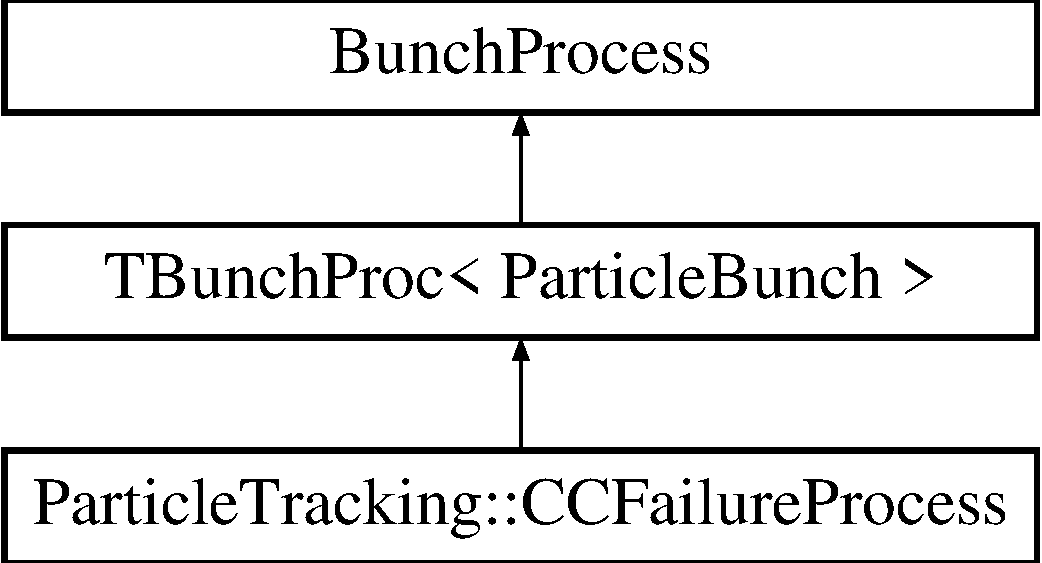
\includegraphics[height=3.000000cm]{classParticleTracking_1_1CCFailureProcess}
\end{center}
\end{figure}
\subsection*{Public Member Functions}
\begin{DoxyCompactItemize}
\item 
\mbox{\Hypertarget{classParticleTracking_1_1CCFailureProcess_a171576b7a0b0e136c7041361e657c766}\label{classParticleTracking_1_1CCFailureProcess_a171576b7a0b0e136c7041361e657c766}} 
{\bfseries C\+C\+Failure\+Process} (int priority, int mode, \hyperlink{classAcceleratorModel}{Accelerator\+Model} $\ast$model, \hyperlink{classLatticeFunctionTable}{Lattice\+Function\+Table} $\ast$twiss)
\item 
\mbox{\Hypertarget{classParticleTracking_1_1CCFailureProcess_ae6436ce8a7eca4a56f2fa2e7158d0354}\label{classParticleTracking_1_1CCFailureProcess_ae6436ce8a7eca4a56f2fa2e7158d0354}} 
{\bfseries C\+C\+Failure\+Process} (int priority, int mode, \hyperlink{classAcceleratorModel}{Accelerator\+Model} $\ast$model, \hyperlink{classLatticeFunctionTable}{Lattice\+Function\+Table} $\ast$twiss, double freq, double crossing, double phase)
\item 
\mbox{\Hypertarget{classParticleTracking_1_1CCFailureProcess_a261a44ddfc6788d6bb662a302a4a048e}\label{classParticleTracking_1_1CCFailureProcess_a261a44ddfc6788d6bb662a302a4a048e}} 
{\bfseries C\+C\+Failure\+Process} (int priority, int mode, \hyperlink{classAcceleratorModel}{Accelerator\+Model} $\ast$model, \hyperlink{classLatticeFunctionTable}{Lattice\+Function\+Table} $\ast$twiss, double freq, double crossing, double phase, int non\+\_\+fail\+\_\+turn, int fail\+\_\+turn)
\item 
\mbox{\Hypertarget{classParticleTracking_1_1CCFailureProcess_a06335f46c5ba7832146e63e2a3dcf654}\label{classParticleTracking_1_1CCFailureProcess_a06335f46c5ba7832146e63e2a3dcf654}} 
virtual void {\bfseries Initialise\+Process} (\hyperlink{classBunch}{Bunch} \&bunch)
\item 
\mbox{\Hypertarget{classParticleTracking_1_1CCFailureProcess_aa44d30217e3f47d96db39466b3842739}\label{classParticleTracking_1_1CCFailureProcess_aa44d30217e3f47d96db39466b3842739}} 
virtual void {\bfseries Set\+Current\+Component} (\hyperlink{classAcceleratorComponent}{Accelerator\+Component} \&component)
\item 
\mbox{\Hypertarget{classParticleTracking_1_1CCFailureProcess_aa82ef6c532bfb74a99650dcc621eac9e}\label{classParticleTracking_1_1CCFailureProcess_aa82ef6c532bfb74a99650dcc621eac9e}} 
virtual void {\bfseries Do\+Process} (double ds)
\item 
\mbox{\Hypertarget{classParticleTracking_1_1CCFailureProcess_a7f8667dc8441f0fe57df127700b79606}\label{classParticleTracking_1_1CCFailureProcess_a7f8667dc8441f0fe57df127700b79606}} 
virtual double {\bfseries Get\+Max\+Allowed\+Step\+Size} () const
\item 
\mbox{\Hypertarget{classParticleTracking_1_1CCFailureProcess_adc086c1b44548ee89004c64b4a7d9e18}\label{classParticleTracking_1_1CCFailureProcess_adc086c1b44548ee89004c64b4a7d9e18}} 
virtual double {\bfseries Calc\+M\+\_\+12} (int start, int end, double deltamu, bool horizontal)
\item 
\mbox{\Hypertarget{classParticleTracking_1_1CCFailureProcess_af94d94452a58b029a4a916e475c1e5e2}\label{classParticleTracking_1_1CCFailureProcess_af94d94452a58b029a4a916e475c1e5e2}} 
virtual double {\bfseries Calc\+M\+\_\+22} (int start, int end, double deltamu, bool horizontal)
\item 
\mbox{\Hypertarget{classParticleTracking_1_1CCFailureProcess_a2bb5e086e48d9f47d88a4f5d7357470d}\label{classParticleTracking_1_1CCFailureProcess_a2bb5e086e48d9f47d88a4f5d7357470d}} 
virtual double {\bfseries Calc\+M\+\_\+12} (int start, int end, bool horizontal)
\item 
\mbox{\Hypertarget{classParticleTracking_1_1CCFailureProcess_aefd15e7f80af1811e19e8e813279c31a}\label{classParticleTracking_1_1CCFailureProcess_aefd15e7f80af1811e19e8e813279c31a}} 
virtual double {\bfseries Calc\+M\+\_\+22} (int start, int end, bool horizontal)
\item 
\mbox{\Hypertarget{classParticleTracking_1_1CCFailureProcess_acf1f4eb29fed5c90248291eb554e60a1}\label{classParticleTracking_1_1CCFailureProcess_acf1f4eb29fed5c90248291eb554e60a1}} 
virtual pair$<$ double, double $>$ {\bfseries Calc\+Mu} (int element)
\item 
\mbox{\Hypertarget{classParticleTracking_1_1CCFailureProcess_aecf310c2335ed1b0ced8e24025ad55bf}\label{classParticleTracking_1_1CCFailureProcess_aecf310c2335ed1b0ced8e24025ad55bf}} 
virtual pair$<$ double, double $>$ {\bfseries Calc\+Delta\+Mu} (int element1, int element2)
\item 
\mbox{\Hypertarget{classParticleTracking_1_1CCFailureProcess_acdf305adc230d6c2fd19e5d503151bc5}\label{classParticleTracking_1_1CCFailureProcess_acdf305adc230d6c2fd19e5d503151bc5}} 
virtual double {\bfseries Calc\+V1} (double M12)
\item 
\mbox{\Hypertarget{classParticleTracking_1_1CCFailureProcess_a4531684518c8196140b868e80bbf7973}\label{classParticleTracking_1_1CCFailureProcess_a4531684518c8196140b868e80bbf7973}} 
virtual double {\bfseries Calc\+V1} (double deltamu, int n1, int n2, bool horizontal)
\item 
\mbox{\Hypertarget{classParticleTracking_1_1CCFailureProcess_a5f3f22a7613e9ec6c6e0bbe92753027b}\label{classParticleTracking_1_1CCFailureProcess_a5f3f22a7613e9ec6c6e0bbe92753027b}} 
virtual double {\bfseries Calc\+V2} (double V1, double M22)
\item 
\mbox{\Hypertarget{classParticleTracking_1_1CCFailureProcess_ac0f155202d76cc1c521b3126def5e1a0}\label{classParticleTracking_1_1CCFailureProcess_ac0f155202d76cc1c521b3126def5e1a0}} 
virtual void {\bfseries Apply\+Pre\+C\+C\+Kick} (\hyperlink{classPSvector}{P\+Svector} \&p, double V, double M12, bool horizontal)
\item 
\mbox{\Hypertarget{classParticleTracking_1_1CCFailureProcess_a40f00d034e33703c0825428b974ff585}\label{classParticleTracking_1_1CCFailureProcess_a40f00d034e33703c0825428b974ff585}} 
virtual void {\bfseries Apply\+Post\+C\+C\+Kick} (\hyperlink{classPSvector}{P\+Svector} \&p, double V, double M12, bool horizontal)
\item 
\mbox{\Hypertarget{classParticleTracking_1_1CCFailureProcess_a5fc3da714963b381a84e8fad8ad301b8}\label{classParticleTracking_1_1CCFailureProcess_a5fc3da714963b381a84e8fad8ad301b8}} 
virtual void {\bfseries Set\+Failure\+On\+Off} (bool onoff)
\item 
\mbox{\Hypertarget{classParticleTracking_1_1CCFailureProcess_abb6bbf06ce70c224d428f32282d3dc4a}\label{classParticleTracking_1_1CCFailureProcess_abb6bbf06ce70c224d428f32282d3dc4a}} 
virtual void {\bfseries Set\+Failure\+Turns} (int ft)
\item 
\mbox{\Hypertarget{classParticleTracking_1_1CCFailureProcess_af537977e29d771616b53f85d3d20b712}\label{classParticleTracking_1_1CCFailureProcess_af537977e29d771616b53f85d3d20b712}} 
virtual void {\bfseries Set\+Non\+Failure\+Turns} (int nft)
\item 
\mbox{\Hypertarget{classParticleTracking_1_1CCFailureProcess_ab816440403837c79221b8a71049ce982}\label{classParticleTracking_1_1CCFailureProcess_ab816440403837c79221b8a71049ce982}} 
virtual void {\bfseries Set\+Failure\+Planes} (bool hor, bool ver)
\end{DoxyCompactItemize}
\subsection*{Additional Inherited Members}


The documentation for this class was generated from the following files\+:\begin{DoxyCompactItemize}
\item 
/home/fallon/git/merlin-\/cmake/\+Merlin/C\+C\+Failure\+Process.\+h\item 
/home/fallon/git/merlin-\/cmake/\+Merlin/C\+C\+Failure\+Process.\+cpp\end{DoxyCompactItemize}

\hypertarget{classCenteredGeometry}{}\section{Centered\+Geometry Class Reference}
\label{classCenteredGeometry}\index{Centered\+Geometry@{Centered\+Geometry}}
Inheritance diagram for Centered\+Geometry\+:\begin{figure}[H]
\begin{center}
\leavevmode
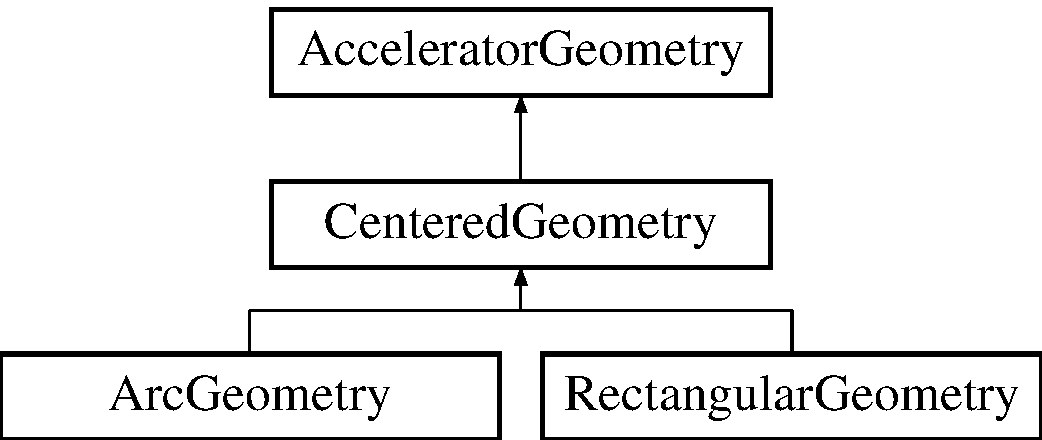
\includegraphics[height=3.000000cm]{classCenteredGeometry}
\end{center}
\end{figure}
\subsection*{Public Member Functions}
\begin{DoxyCompactItemize}
\item 
\mbox{\Hypertarget{classCenteredGeometry_a3326b5b4b276ef6e7c277ad29d675dbb}\label{classCenteredGeometry_a3326b5b4b276ef6e7c277ad29d675dbb}} 
{\bfseries Centered\+Geometry} (double l)
\item 
virtual double \hyperlink{classCenteredGeometry_afe03a287567dec16f8663f4211f82add}{Get\+Geometry\+Length} () const
\item 
virtual Accelerator\+Geometry\+::\+Extent \hyperlink{classCenteredGeometry_abd27afe15472ebd057d0b60f1d531a1a}{Get\+Geometry\+Extent} () const
\end{DoxyCompactItemize}
\subsection*{Protected Member Functions}
\begin{DoxyCompactItemize}
\item 
\mbox{\Hypertarget{classCenteredGeometry_ad3cf5fb2053fa2122b1b2853ad54b88f}\label{classCenteredGeometry_ad3cf5fb2053fa2122b1b2853ad54b88f}} 
void {\bfseries Check\+Bounds} (double s1, double s2) const
\item 
\mbox{\Hypertarget{classCenteredGeometry_ae17b8865d0b86aa6cc2b391bf3eff7a3}\label{classCenteredGeometry_ae17b8865d0b86aa6cc2b391bf3eff7a3}} 
void {\bfseries Check\+Bounds} (double s) const
\end{DoxyCompactItemize}
\subsection*{Protected Attributes}
\begin{DoxyCompactItemize}
\item 
\mbox{\Hypertarget{classCenteredGeometry_a0e05846708a78529814ed74b1ec6a2cb}\label{classCenteredGeometry_a0e05846708a78529814ed74b1ec6a2cb}} 
double {\bfseries len}
\end{DoxyCompactItemize}
\subsection*{Additional Inherited Members}


\subsection{Member Function Documentation}
\mbox{\Hypertarget{classCenteredGeometry_abd27afe15472ebd057d0b60f1d531a1a}\label{classCenteredGeometry_abd27afe15472ebd057d0b60f1d531a1a}} 
\index{Centered\+Geometry@{Centered\+Geometry}!Get\+Geometry\+Extent@{Get\+Geometry\+Extent}}
\index{Get\+Geometry\+Extent@{Get\+Geometry\+Extent}!Centered\+Geometry@{Centered\+Geometry}}
\subsubsection{\texorpdfstring{Get\+Geometry\+Extent()}{GetGeometryExtent()}}
{\footnotesize\ttfamily Accelerator\+Geometry\+::\+Extent Centered\+Geometry\+::\+Get\+Geometry\+Extent (\begin{DoxyParamCaption}{ }\end{DoxyParamCaption}) const\hspace{0.3cm}{\ttfamily [inline]}, {\ttfamily [virtual]}}

Returns the local extent of this geometry. \begin{DoxyReturn}{Returns}
A pair giving the extent of this geometry. 
\end{DoxyReturn}


Implements \hyperlink{classAcceleratorGeometry_a2db830fe927af3c9cba59b8452370bfb}{Accelerator\+Geometry}.

\mbox{\Hypertarget{classCenteredGeometry_afe03a287567dec16f8663f4211f82add}\label{classCenteredGeometry_afe03a287567dec16f8663f4211f82add}} 
\index{Centered\+Geometry@{Centered\+Geometry}!Get\+Geometry\+Length@{Get\+Geometry\+Length}}
\index{Get\+Geometry\+Length@{Get\+Geometry\+Length}!Centered\+Geometry@{Centered\+Geometry}}
\subsubsection{\texorpdfstring{Get\+Geometry\+Length()}{GetGeometryLength()}}
{\footnotesize\ttfamily double Centered\+Geometry\+::\+Get\+Geometry\+Length (\begin{DoxyParamCaption}{ }\end{DoxyParamCaption}) const\hspace{0.3cm}{\ttfamily [inline]}, {\ttfamily [virtual]}}

Returns the total arc-\/length of the geometry. \begin{DoxyReturn}{Returns}
A double giving the total length of this geometry. 
\end{DoxyReturn}


Implements \hyperlink{classAcceleratorGeometry_abc36f96d542e0d9db592f8e7ee455769}{Accelerator\+Geometry}.



The documentation for this class was generated from the following file\+:\begin{DoxyCompactItemize}
\item 
/home/fallon/git/merlin-\/cmake/\+Merlin/Centered\+Geometry.\+h\end{DoxyCompactItemize}

\hypertarget{classChannelServer_1_1ChannelCtor}{}\section{Channel\+Server\+:\+:Channel\+Ctor Class Reference}
\label{classChannelServer_1_1ChannelCtor}\index{Channel\+Server\+::\+Channel\+Ctor@{Channel\+Server\+::\+Channel\+Ctor}}
Inheritance diagram for Channel\+Server\+:\+:Channel\+Ctor\+:\begin{figure}[H]
\begin{center}
\leavevmode
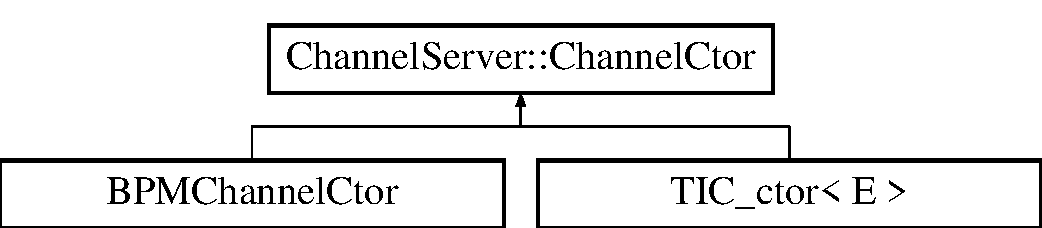
\includegraphics[height=2.000000cm]{classChannelServer_1_1ChannelCtor}
\end{center}
\end{figure}
\subsection*{Public Member Functions}
\begin{DoxyCompactItemize}
\item 
\mbox{\Hypertarget{classChannelServer_1_1ChannelCtor_a682cb384c9d734a4f5d5299b26df312e}\label{classChannelServer_1_1ChannelCtor_a682cb384c9d734a4f5d5299b26df312e}} 
virtual \hyperlink{classROChannel}{R\+O\+Channel} $\ast$ {\bfseries Construct\+RO} (\hyperlink{classModelElement}{Model\+Element} $\ast$an\+Element)=0
\item 
\mbox{\Hypertarget{classChannelServer_1_1ChannelCtor_af75ca12bf26102eacb1e8a729ff3690b}\label{classChannelServer_1_1ChannelCtor_af75ca12bf26102eacb1e8a729ff3690b}} 
virtual \hyperlink{classRWChannel}{R\+W\+Channel} $\ast$ {\bfseries Construct\+RW} (\hyperlink{classModelElement}{Model\+Element} $\ast$an\+Element)=0
\item 
\mbox{\Hypertarget{classChannelServer_1_1ChannelCtor_ad1ef45766e2c8d83033db9c3170d0a1b}\label{classChannelServer_1_1ChannelCtor_ad1ef45766e2c8d83033db9c3170d0a1b}} 
std\+::string {\bfseries Get\+ID} ()
\item 
\mbox{\Hypertarget{classChannelServer_1_1ChannelCtor_af2e88064ee9b1d1a02e31b59aaf8700b}\label{classChannelServer_1_1ChannelCtor_af2e88064ee9b1d1a02e31b59aaf8700b}} 
const string \& {\bfseries Get\+Type} () const
\item 
\mbox{\Hypertarget{classChannelServer_1_1ChannelCtor_a6aacf865e0d9b04e70da858458662656}\label{classChannelServer_1_1ChannelCtor_a6aacf865e0d9b04e70da858458662656}} 
const string \& {\bfseries Get\+Key} () const
\end{DoxyCompactItemize}
\subsection*{Protected Member Functions}
\begin{DoxyCompactItemize}
\item 
\mbox{\Hypertarget{classChannelServer_1_1ChannelCtor_a90a2a06743e7e77bd59135e3835fcda0}\label{classChannelServer_1_1ChannelCtor_a90a2a06743e7e77bd59135e3835fcda0}} 
{\bfseries Channel\+Ctor} (const string \&a\+Type, const string \&a\+Key)
\end{DoxyCompactItemize}
\subsection*{Protected Attributes}
\begin{DoxyCompactItemize}
\item 
\mbox{\Hypertarget{classChannelServer_1_1ChannelCtor_a07645ac6a004b22887e5631cd3a9cbc9}\label{classChannelServer_1_1ChannelCtor_a07645ac6a004b22887e5631cd3a9cbc9}} 
std\+::string {\bfseries type}
\item 
\mbox{\Hypertarget{classChannelServer_1_1ChannelCtor_af1452bd1601ae3b9dff497745fa162b7}\label{classChannelServer_1_1ChannelCtor_af1452bd1601ae3b9dff497745fa162b7}} 
std\+::string {\bfseries key}
\end{DoxyCompactItemize}


The documentation for this class was generated from the following files\+:\begin{DoxyCompactItemize}
\item 
/home/fallon/git/merlin-\/cmake/\+Merlin/Channel\+Server.\+h\item 
/home/fallon/git/merlin-\/cmake/\+Merlin/Channel\+Server.\+cpp\end{DoxyCompactItemize}

\hypertarget{classChannelServer}{}\section{Channel\+Server Class Reference}
\label{classChannelServer}\index{Channel\+Server@{Channel\+Server}}
\subsection*{Classes}
\begin{DoxyCompactItemize}
\item 
class \hyperlink{classChannelServer_1_1ChannelCtor}{Channel\+Ctor}
\end{DoxyCompactItemize}
\subsection*{Public Types}
\begin{DoxyCompactItemize}
\item 
\mbox{\Hypertarget{classChannelServer_adde1c6e4f0cac691b23c8746cea7e7b6}\label{classChannelServer_adde1c6e4f0cac691b23c8746cea7e7b6}} 
typedef std\+::map$<$ std\+::string, \hyperlink{classChannelServer_1_1ChannelCtor}{Channel\+Ctor} $\ast$ $>$ {\bfseries Ctor\+Table}
\end{DoxyCompactItemize}
\subsection*{Public Member Functions}
\begin{DoxyCompactItemize}
\item 
\mbox{\Hypertarget{classChannelServer_a2974f5201de153453cef0f778f0b0914}\label{classChannelServer_a2974f5201de153453cef0f778f0b0914}} 
size\+\_\+t {\bfseries Get\+R\+O\+Channels} (const string \&ch\+ID, std\+::vector$<$ \hyperlink{classROChannel}{R\+O\+Channel} $\ast$$>$ \&channels)
\item 
\mbox{\Hypertarget{classChannelServer_aebd556c35a30e712ce4024f500b0b1fb}\label{classChannelServer_aebd556c35a30e712ce4024f500b0b1fb}} 
size\+\_\+t {\bfseries Get\+R\+W\+Channels} (const string \&ch\+ID, std\+::vector$<$ \hyperlink{classRWChannel}{R\+W\+Channel} $\ast$$>$ \&channels)
\item 
\mbox{\Hypertarget{classChannelServer_ac2ba111c261a2962216be8d494d1f09b}\label{classChannelServer_ac2ba111c261a2962216be8d494d1f09b}} 
size\+\_\+t {\bfseries Get\+R\+O\+Channels} (\hyperlink{classAcceleratorModel_1_1Beamline}{Accelerator\+Model\+::\+Beamline} \&a\+Beamline, const std\+::string \&chid, std\+::vector$<$ \hyperlink{classROChannel}{R\+O\+Channel} $\ast$$>$ \&channels)
\item 
\mbox{\Hypertarget{classChannelServer_a6e0745f0faadfc8597c76bb208dd40d1}\label{classChannelServer_a6e0745f0faadfc8597c76bb208dd40d1}} 
size\+\_\+t {\bfseries Get\+R\+W\+Channels} (\hyperlink{classAcceleratorModel_1_1Beamline}{Accelerator\+Model\+::\+Beamline} \&a\+Beamline, const std\+::string \&chid, std\+::vector$<$ \hyperlink{classRWChannel}{R\+W\+Channel} $\ast$$>$ \&channels)
\item 
\mbox{\Hypertarget{classChannelServer_a15dadfefbf4ebb41db8f1c6db8f85b6f}\label{classChannelServer_a15dadfefbf4ebb41db8f1c6db8f85b6f}} 
void {\bfseries Register\+Ctor} (\hyperlink{classChannelServer_1_1ChannelCtor}{Channel\+Ctor} $\ast$chctor)
\item 
\mbox{\Hypertarget{classChannelServer_a73ce366d47580f069d4c44fcf2835d1d}\label{classChannelServer_a73ce366d47580f069d4c44fcf2835d1d}} 
void {\bfseries Set\+Repository} (\hyperlink{classElementRepository}{Element\+Repository} $\ast$me\+\_\+repo)
\end{DoxyCompactItemize}


The documentation for this class was generated from the following files\+:\begin{DoxyCompactItemize}
\item 
/home/fallon/git/merlin-\/cmake/\+Merlin/Channel\+Server.\+h\item 
/home/fallon/git/merlin-\/cmake/\+Merlin/Channel\+Server.\+cpp\end{DoxyCompactItemize}

\hypertarget{classCircularAperture}{}\section{Circular\+Aperture Class Reference}
\label{classCircularAperture}\index{Circular\+Aperture@{Circular\+Aperture}}


{\ttfamily \#include $<$Simple\+Apertures.\+h$>$}

Inheritance diagram for Circular\+Aperture\+:\begin{figure}[H]
\begin{center}
\leavevmode
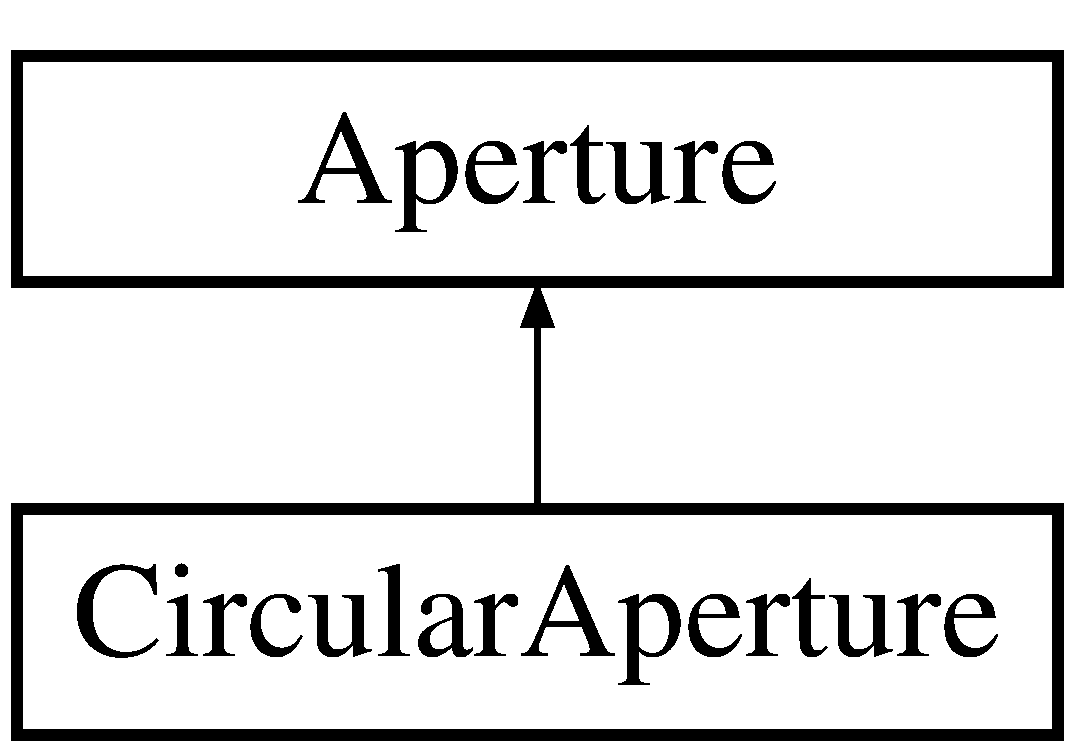
\includegraphics[height=2.000000cm]{classCircularAperture}
\end{center}
\end{figure}
\subsection*{Public Member Functions}
\begin{DoxyCompactItemize}
\item 
\mbox{\Hypertarget{classCircularAperture_ab762f5d7bdfd14133a3c638736842aae}\label{classCircularAperture_ab762f5d7bdfd14133a3c638736842aae}} 
{\bfseries Circular\+Aperture} (double r)
\item 
\mbox{\Hypertarget{classCircularAperture_aeb06ebc0f40d863ce9e8d062bf27e20f}\label{classCircularAperture_aeb06ebc0f40d863ce9e8d062bf27e20f}} 
double {\bfseries Get\+Radius} () const
\item 
\mbox{\Hypertarget{classCircularAperture_a8b4384aa00bc5da6c88b7f0132554e19}\label{classCircularAperture_a8b4384aa00bc5da6c88b7f0132554e19}} 
double {\bfseries Get\+Diameter} () const
\item 
\mbox{\Hypertarget{classCircularAperture_a4702c029c5be632e94301bb76a99a428}\label{classCircularAperture_a4702c029c5be632e94301bb76a99a428}} 
void {\bfseries Set\+Radius} (double r)
\item 
\mbox{\Hypertarget{classCircularAperture_a952ec2c24dec60e01e8efec258b979f5}\label{classCircularAperture_a952ec2c24dec60e01e8efec258b979f5}} 
void {\bfseries Set\+Diameter} (double d)
\item 
virtual bool \hyperlink{classCircularAperture_a1cc2c7d1ff491dbfb0c24790897d4519}{Point\+Inside} (double x, double y, double z) const
\item 
virtual double \hyperlink{classCircularAperture_ab2f83be4d78bb1495b2b0aebef78e189}{Get\+Radius\+At} (double phi, double z) const
\item 
virtual std\+::string \hyperlink{classCircularAperture_a18f05ba1dde35881014ba3aa2ed693bc}{Get\+Aperture\+Type} () const
\item 
virtual void \hyperlink{classCircularAperture_af7380933fd3494dd0d1868b655a78b08}{printout} (std\+::ostream \&out) const
\end{DoxyCompactItemize}
\subsection*{Additional Inherited Members}


\subsection{Detailed Description}
Represents an aperture with a circular cross-\/section. The aperture is assumed to be extruded along its geometry. 

\subsection{Member Function Documentation}
\mbox{\Hypertarget{classCircularAperture_a18f05ba1dde35881014ba3aa2ed693bc}\label{classCircularAperture_a18f05ba1dde35881014ba3aa2ed693bc}} 
\index{Circular\+Aperture@{Circular\+Aperture}!Get\+Aperture\+Type@{Get\+Aperture\+Type}}
\index{Get\+Aperture\+Type@{Get\+Aperture\+Type}!Circular\+Aperture@{Circular\+Aperture}}
\subsubsection{\texorpdfstring{Get\+Aperture\+Type()}{GetApertureType()}}
{\footnotesize\ttfamily std\+::string Circular\+Aperture\+::\+Get\+Aperture\+Type (\begin{DoxyParamCaption}{ }\end{DoxyParamCaption}) const\hspace{0.3cm}{\ttfamily [inline]}, {\ttfamily [virtual]}}

Returns the type of the aperture. \begin{DoxyReturn}{Returns}
A string containing the type of the aperture. 
\end{DoxyReturn}


Implements \hyperlink{classAperture_ad7af612271a0586feea83c38549dfb75}{Aperture}.

\mbox{\Hypertarget{classCircularAperture_ab2f83be4d78bb1495b2b0aebef78e189}\label{classCircularAperture_ab2f83be4d78bb1495b2b0aebef78e189}} 
\index{Circular\+Aperture@{Circular\+Aperture}!Get\+Radius\+At@{Get\+Radius\+At}}
\index{Get\+Radius\+At@{Get\+Radius\+At}!Circular\+Aperture@{Circular\+Aperture}}
\subsubsection{\texorpdfstring{Get\+Radius\+At()}{GetRadiusAt()}}
{\footnotesize\ttfamily double Circular\+Aperture\+::\+Get\+Radius\+At (\begin{DoxyParamCaption}\item[{double}]{phi,  }\item[{double}]{z }\end{DoxyParamCaption}) const\hspace{0.3cm}{\ttfamily [virtual]}}

Returns the radius.

Circular \hyperlink{classAperture}{Aperture} Functions 

Implements \hyperlink{classAperture_ad0ea7907d393ec1e6a8303343fe9dd29}{Aperture}.

\mbox{\Hypertarget{classCircularAperture_a1cc2c7d1ff491dbfb0c24790897d4519}\label{classCircularAperture_a1cc2c7d1ff491dbfb0c24790897d4519}} 
\index{Circular\+Aperture@{Circular\+Aperture}!Point\+Inside@{Point\+Inside}}
\index{Point\+Inside@{Point\+Inside}!Circular\+Aperture@{Circular\+Aperture}}
\subsubsection{\texorpdfstring{Point\+Inside()}{PointInside()}}
{\footnotesize\ttfamily bool Circular\+Aperture\+::\+Point\+Inside (\begin{DoxyParamCaption}\item[{double}]{x,  }\item[{double}]{y,  }\item[{double}]{z }\end{DoxyParamCaption}) const\hspace{0.3cm}{\ttfamily [inline]}, {\ttfamily [virtual]}}

Returns true if the point (x,y,z) is within the aperture. The z coordinate is ignored. 

Implements \hyperlink{classAperture_a77854d058bf8a00cfeb7a6d766dc0028}{Aperture}.

\mbox{\Hypertarget{classCircularAperture_af7380933fd3494dd0d1868b655a78b08}\label{classCircularAperture_af7380933fd3494dd0d1868b655a78b08}} 
\index{Circular\+Aperture@{Circular\+Aperture}!printout@{printout}}
\index{printout@{printout}!Circular\+Aperture@{Circular\+Aperture}}
\subsubsection{\texorpdfstring{printout()}{printout()}}
{\footnotesize\ttfamily void Circular\+Aperture\+::printout (\begin{DoxyParamCaption}\item[{std\+::ostream \&}]{out }\end{DoxyParamCaption}) const\hspace{0.3cm}{\ttfamily [virtual]}}

Prints out the \hyperlink{classAperture}{Aperture} parameters to a specified stream. 
\begin{DoxyParams}[1]{Parameters}
\mbox{\tt out}  & {\em out} & The output stream to use. \\
\hline
\end{DoxyParams}


Reimplemented from \hyperlink{classAperture_aff2f276b93bb2cb94e559e1c4901e38e}{Aperture}.



The documentation for this class was generated from the following files\+:\begin{DoxyCompactItemize}
\item 
/home/fallon/git/merlin-\/cmake/\+Merlin/Simple\+Apertures.\+h\item 
/home/fallon/git/merlin-\/cmake/\+Merlin/Simple\+Apertures.\+cpp\end{DoxyCompactItemize}

\hypertarget{structClearLatticeFunction}{}\section{Clear\+Lattice\+Function Struct Reference}
\label{structClearLatticeFunction}\index{Clear\+Lattice\+Function@{Clear\+Lattice\+Function}}
\subsection*{Public Member Functions}
\begin{DoxyCompactItemize}
\item 
\mbox{\Hypertarget{structClearLatticeFunction_ae0601e470e3d9cbe56d8793e735f29c1}\label{structClearLatticeFunction_ae0601e470e3d9cbe56d8793e735f29c1}} 
void {\bfseries operator()} (\hyperlink{classLatticeFunction}{Lattice\+Function} $\ast$lfn)
\end{DoxyCompactItemize}


The documentation for this struct was generated from the following file\+:\begin{DoxyCompactItemize}
\item 
/home/fallon/git/merlin-\/cmake/\+Merlin/Lattice\+Functions.\+cpp\end{DoxyCompactItemize}

\hypertarget{classClosedOrbit}{}\section{Closed\+Orbit Class Reference}
\label{classClosedOrbit}\index{Closed\+Orbit@{Closed\+Orbit}}
\subsection*{Public Member Functions}
\begin{DoxyCompactItemize}
\item 
\mbox{\Hypertarget{classClosedOrbit_afbbe124fdc603de514cce959fc90db02}\label{classClosedOrbit_afbbe124fdc603de514cce959fc90db02}} 
{\bfseries Closed\+Orbit} (\hyperlink{classAcceleratorModel}{Accelerator\+Model} $\ast$a\+Model, double ref\+Momentum)
\item 
\mbox{\Hypertarget{classClosedOrbit_ace9fda3eec47500e4a1ff0d5e301020c}\label{classClosedOrbit_ace9fda3eec47500e4a1ff0d5e301020c}} 
void {\bfseries Find\+Closed\+Orbit} (\hyperlink{classPSvector}{P\+Svector} \&particle, int ncpt=0)
\item 
\mbox{\Hypertarget{classClosedOrbit_aca682dc3a765e0c329593105e03da6ed}\label{classClosedOrbit_aca682dc3a765e0c329593105e03da6ed}} 
void {\bfseries Find\+R\+M\+S\+Orbit} (\hyperlink{classPSvector}{P\+Svector} \&particle)
\item 
\mbox{\Hypertarget{classClosedOrbit_a5227f58329058be8e35a060eb6721e31}\label{classClosedOrbit_a5227f58329058be8e35a060eb6721e31}} 
void {\bfseries Transverse\+Only} (bool flag)
\item 
\mbox{\Hypertarget{classClosedOrbit_a87667981d76fec5dce8ec8d213fa0739}\label{classClosedOrbit_a87667981d76fec5dce8ec8d213fa0739}} 
void {\bfseries Radiation} (bool flag)
\item 
\mbox{\Hypertarget{classClosedOrbit_aeb1d11fe50153fd03912e2a890669acb}\label{classClosedOrbit_aeb1d11fe50153fd03912e2a890669acb}} 
void {\bfseries Set\+Rad\+Step\+Size} (double rad\+\_\+stepsize)
\item 
\mbox{\Hypertarget{classClosedOrbit_ac0f99b1c811c309f41632c12a77cd68d}\label{classClosedOrbit_ac0f99b1c811c309f41632c12a77cd68d}} 
void {\bfseries Set\+Rad\+Num\+Steps} (int rad\+\_\+numsteps)
\item 
\mbox{\Hypertarget{classClosedOrbit_a9b77f7e8be310ffbb305a9c0b426c16e}\label{classClosedOrbit_a9b77f7e8be310ffbb305a9c0b426c16e}} 
void {\bfseries Full\+Acceleration} (bool flag)
\item 
\mbox{\Hypertarget{classClosedOrbit_a66bccb6696d84ae18835d1ba026f6d8a}\label{classClosedOrbit_a66bccb6696d84ae18835d1ba026f6d8a}} 
void {\bfseries Scale\+Bend\+Path\+Length} (double scale)
\item 
\mbox{\Hypertarget{classClosedOrbit_a959f43e822fde678d95b995050158e1f}\label{classClosedOrbit_a959f43e822fde678d95b995050158e1f}} 
void {\bfseries Set\+Delta} (double new\+\_\+delta)
\item 
\mbox{\Hypertarget{classClosedOrbit_a4894fdac476b86f3f9aacbe17b074d51}\label{classClosedOrbit_a4894fdac476b86f3f9aacbe17b074d51}} 
void {\bfseries Set\+Tolerance} (double tolerance)
\item 
\mbox{\Hypertarget{classClosedOrbit_ac8ed5c9d59bd8bf305595773ad993058}\label{classClosedOrbit_ac8ed5c9d59bd8bf305595773ad993058}} 
void {\bfseries Set\+Max\+Iterations} (int max\+\_\+iterations)
\item 
\mbox{\Hypertarget{classClosedOrbit_a88194e65d537025263bf7df39b8c2045}\label{classClosedOrbit_a88194e65d537025263bf7df39b8c2045}} 
void {\bfseries Add\+Process} (\hyperlink{classTBunchProc}{Particle\+Bunch\+Process} $\ast$a\+Process)
\end{DoxyCompactItemize}
\subsection*{Public Attributes}
\begin{DoxyCompactItemize}
\item 
\mbox{\Hypertarget{classClosedOrbit_a2a375e532a8603a0e97b8819b7b770bb}\label{classClosedOrbit_a2a375e532a8603a0e97b8819b7b770bb}} 
double {\bfseries w}
\item 
\mbox{\Hypertarget{classClosedOrbit_aea27444278158b7a5ecc0e43e619bf9a}\label{classClosedOrbit_aea27444278158b7a5ecc0e43e619bf9a}} 
int {\bfseries iter}
\end{DoxyCompactItemize}


The documentation for this class was generated from the following files\+:\begin{DoxyCompactItemize}
\item 
/home/fallon/git/merlin-\/cmake/\+Merlin/Closed\+Orbit.\+h\item 
/home/fallon/git/merlin-\/cmake/\+Merlin/Closed\+Orbit.\+cpp\end{DoxyCompactItemize}

\hypertarget{classParticleTracking_1_1CollimateParticleProcess}{}\section{Particle\+Tracking\+:\+:Collimate\+Particle\+Process Class Reference}
\label{classParticleTracking_1_1CollimateParticleProcess}\index{Particle\+Tracking\+::\+Collimate\+Particle\+Process@{Particle\+Tracking\+::\+Collimate\+Particle\+Process}}


{\ttfamily \#include $<$Collimate\+Particle\+Process.\+h$>$}

Inheritance diagram for Particle\+Tracking\+:\+:Collimate\+Particle\+Process\+:\begin{figure}[H]
\begin{center}
\leavevmode
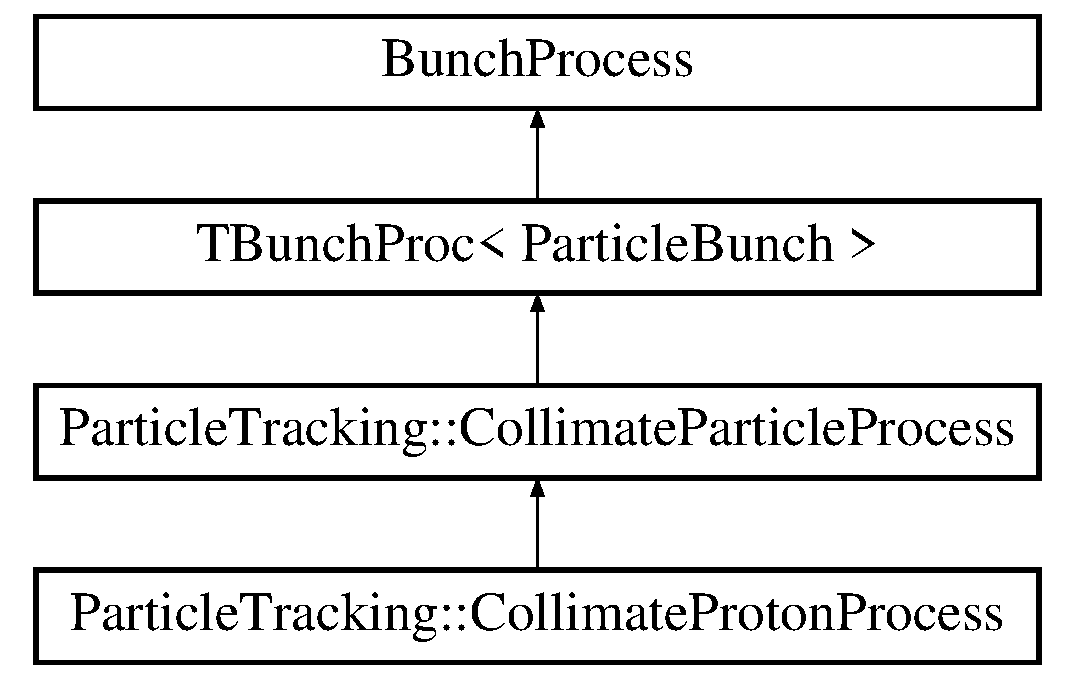
\includegraphics[height=4.000000cm]{classParticleTracking_1_1CollimateParticleProcess}
\end{center}
\end{figure}
\subsection*{Public Types}
\begin{DoxyCompactItemize}
\item 
typedef map$<$ string, int $>$ \hyperlink{classParticleTracking_1_1CollimateParticleProcess_ac2ecc4232755ca120567b420af5b1dc8}{I\+D\+T\+BL}
\end{DoxyCompactItemize}
\subsection*{Public Member Functions}
\begin{DoxyCompactItemize}
\item 
\hyperlink{classParticleTracking_1_1CollimateParticleProcess_ae93c881a9b08429d74a06627c55d4cd4}{Collimate\+Particle\+Process} (int priority, int mode, std\+::ostream $\ast$osp=nullptr)
\item 
virtual void \hyperlink{classParticleTracking_1_1CollimateParticleProcess_a884a7d80cda58ee50cdaa4ec2fb56b62}{Initialise\+Process} (\hyperlink{classBunch}{Bunch} \&bunch)
\item 
virtual void \hyperlink{classParticleTracking_1_1CollimateParticleProcess_ab3f22a0f67414d883f33e39dab7d763b}{Set\+Current\+Component} (\hyperlink{classAcceleratorComponent}{Accelerator\+Component} \&component)
\item 
virtual void \hyperlink{classParticleTracking_1_1CollimateParticleProcess_a0e987f9ad599b59c82751cceff1b97f9}{Do\+Process} (double ds)
\item 
virtual double \hyperlink{classParticleTracking_1_1CollimateParticleProcess_a26262dec26f0c35658a2a968a1583b81}{Get\+Max\+Allowed\+Step\+Size} () const
\item 
void \hyperlink{classParticleTracking_1_1CollimateParticleProcess_a6ce4a520f7eb912bdfa635ef26614733}{Scatter\+At\+Collimator} (bool tf)
\item 
void \hyperlink{classParticleTracking_1_1CollimateParticleProcess_a621e89e37cda11077f18dc3ff4980de8}{Create\+Particle\+Loss\+Files} (bool flg, string fprefix=\char`\"{}\char`\"{})
\item 
void \hyperlink{classParticleTracking_1_1CollimateParticleProcess_ab6d43f1bec63763099ef71a003ceaef4}{Index\+Particles} (bool index)
\item 
\mbox{\Hypertarget{classParticleTracking_1_1CollimateParticleProcess_ad048cb54a8e9e365e6102e0b4029aba0}\label{classParticleTracking_1_1CollimateParticleProcess_ad048cb54a8e9e365e6102e0b4029aba0}} 
void {\bfseries Index\+Particles} (std\+::list$<$ size\+\_\+t $>$ \&an\+Index)
\item 
\mbox{\Hypertarget{classParticleTracking_1_1CollimateParticleProcess_a80f6d0e9bbd8afda5e94ddc0d8be4203}\label{classParticleTracking_1_1CollimateParticleProcess_a80f6d0e9bbd8afda5e94ddc0d8be4203}} 
const std\+::list$<$ size\+\_\+t $>$ \& {\bfseries Get\+Indecies} () const
\item 
void \hyperlink{classParticleTracking_1_1CollimateParticleProcess_ae00a6eaeda4b46eb25a1bc28e399b4f8}{Set\+Loss\+Threshold} (double losspc)
\item 
void \hyperlink{classParticleTracking_1_1CollimateParticleProcess_af9bcc2aff428281af1d79011d6978685}{Set\+Log\+Stream} (std\+::ostream $\ast$an\+Os)
\item 
void \hyperlink{classParticleTracking_1_1CollimateParticleProcess_a12c96ec3f91752f211c135f96ba2248c}{Enable\+Imperfections} (bool)
\item 
\mbox{\Hypertarget{classParticleTracking_1_1CollimateParticleProcess_a5fb0f7680678f9301a7328012b4ca345}\label{classParticleTracking_1_1CollimateParticleProcess_a5fb0f7680678f9301a7328012b4ca345}} 
virtual double {\bfseries Get\+Output\+Bin\+Size} () const
\item 
\mbox{\Hypertarget{classParticleTracking_1_1CollimateParticleProcess_aa615fc6c8eb385a5a1d7ff563b64571f}\label{classParticleTracking_1_1CollimateParticleProcess_aa615fc6c8eb385a5a1d7ff563b64571f}} 
virtual void {\bfseries Set\+Output\+Bin\+Size} (double)
\item 
\mbox{\Hypertarget{classParticleTracking_1_1CollimateParticleProcess_ac996f3bfacd5358da92209ca517bf4e3}\label{classParticleTracking_1_1CollimateParticleProcess_ac996f3bfacd5358da92209ca517bf4e3}} 
virtual void {\bfseries Set\+Collimation\+Output} (\hyperlink{classParticleTracking_1_1CollimationOutput}{Collimation\+Output} $\ast$odb)
\end{DoxyCompactItemize}
\subsection*{Public Attributes}
\begin{DoxyCompactItemize}
\item 
\mbox{\Hypertarget{classParticleTracking_1_1CollimateParticleProcess_a4f49392ff553cbadb600c5813ee26c76}\label{classParticleTracking_1_1CollimateParticleProcess_a4f49392ff553cbadb600c5813ee26c76}} 
std\+::vector$<$ \hyperlink{classParticleTracking_1_1CollimationOutput}{Collimation\+Output} $\ast$ $>$ {\bfseries Collimation\+Output\+Vector}
\item 
\mbox{\Hypertarget{classParticleTracking_1_1CollimateParticleProcess_a1da526fdda9ded05c1fa0e6127a6ae85}\label{classParticleTracking_1_1CollimateParticleProcess_a1da526fdda9ded05c1fa0e6127a6ae85}} 
std\+::vector$<$ \hyperlink{classParticleTracking_1_1CollimationOutput}{Collimation\+Output} $\ast$ $>$\+::iterator {\bfseries Collimation\+Output\+Iterator}
\end{DoxyCompactItemize}
\subsection*{Protected Member Functions}
\begin{DoxyCompactItemize}
\item 
\mbox{\Hypertarget{classParticleTracking_1_1CollimateParticleProcess_adc2ef32a6f444a0083b4e44d23441503}\label{classParticleTracking_1_1CollimateParticleProcess_adc2ef32a6f444a0083b4e44d23441503}} 
double {\bfseries Get\+Bin\+Size} () const
\end{DoxyCompactItemize}
\subsection*{Protected Attributes}
\begin{DoxyCompactItemize}
\item 
\mbox{\Hypertarget{classParticleTracking_1_1CollimateParticleProcess_afee90888d5dc01760302786c74ebb5b1}\label{classParticleTracking_1_1CollimateParticleProcess_afee90888d5dc01760302786c74ebb5b1}} 
int {\bfseries cmode}
\item 
\mbox{\Hypertarget{classParticleTracking_1_1CollimateParticleProcess_a1ad8e990f6603de53341ddf8810a5ce0}\label{classParticleTracking_1_1CollimateParticleProcess_a1ad8e990f6603de53341ddf8810a5ce0}} 
std\+::ostream $\ast$ {\bfseries os}
\item 
\mbox{\Hypertarget{classParticleTracking_1_1CollimateParticleProcess_a248fe2a4e249f9f75a8905b2a6bf4584}\label{classParticleTracking_1_1CollimateParticleProcess_a248fe2a4e249f9f75a8905b2a6bf4584}} 
bool {\bfseries create\+Loss\+Files}
\item 
\mbox{\Hypertarget{classParticleTracking_1_1CollimateParticleProcess_a80462e8bff6f6db8a6e3e0b41bdf2d1b}\label{classParticleTracking_1_1CollimateParticleProcess_a80462e8bff6f6db8a6e3e0b41bdf2d1b}} 
string {\bfseries file\+\_\+prefix}
\item 
\mbox{\Hypertarget{classParticleTracking_1_1CollimateParticleProcess_a3302a12aa91cf298e26d956a6addb6b3}\label{classParticleTracking_1_1CollimateParticleProcess_a3302a12aa91cf298e26d956a6addb6b3}} 
double {\bfseries loss\+Threshold}
\item 
\mbox{\Hypertarget{classParticleTracking_1_1CollimateParticleProcess_aba22f330c790e143d7120066544e1dc0}\label{classParticleTracking_1_1CollimateParticleProcess_aba22f330c790e143d7120066544e1dc0}} 
size\+\_\+t {\bfseries nstart}
\item 
\mbox{\Hypertarget{classParticleTracking_1_1CollimateParticleProcess_a0ca088327b33f967861164ffbcecb151}\label{classParticleTracking_1_1CollimateParticleProcess_a0ca088327b33f967861164ffbcecb151}} 
std\+::list$<$ size\+\_\+t $>$ $\ast$ {\bfseries pindex}
\item 
\mbox{\Hypertarget{classParticleTracking_1_1CollimateParticleProcess_ad306056a5b618f3864010d273d17e3ad}\label{classParticleTracking_1_1CollimateParticleProcess_ad306056a5b618f3864010d273d17e3ad}} 
\hyperlink{classParticleTracking_1_1CollimateParticleProcess_ac2ecc4232755ca120567b420af5b1dc8}{I\+D\+T\+BL} {\bfseries idtbl}
\item 
P\+Svector\+Array \hyperlink{classParticleTracking_1_1CollimateParticleProcess_acb74939dca67e8da645bf20aaef0e26c}{Input\+Array}
\item 
\mbox{\Hypertarget{classParticleTracking_1_1CollimateParticleProcess_a8307d83a64674534ecdd944a27db7dfe}\label{classParticleTracking_1_1CollimateParticleProcess_a8307d83a64674534ecdd944a27db7dfe}} 
double {\bfseries s\+\_\+total}
\item 
\mbox{\Hypertarget{classParticleTracking_1_1CollimateParticleProcess_a634bec0a65c8f12e4e90cc022324e665}\label{classParticleTracking_1_1CollimateParticleProcess_a634bec0a65c8f12e4e90cc022324e665}} 
double {\bfseries s}
\item 
\mbox{\Hypertarget{classParticleTracking_1_1CollimateParticleProcess_a5a32a5153ed9d7625fd4aa553440e98d}\label{classParticleTracking_1_1CollimateParticleProcess_a5a32a5153ed9d7625fd4aa553440e98d}} 
double {\bfseries next\+\_\+s}
\item 
double \hyperlink{classParticleTracking_1_1CollimateParticleProcess_aa43743501b217f519067dce6e51b7cae}{len}
\item 
\mbox{\Hypertarget{classParticleTracking_1_1CollimateParticleProcess_a132d2896b273060ded3c90d5a299fae3}\label{classParticleTracking_1_1CollimateParticleProcess_a132d2896b273060ded3c90d5a299fae3}} 
bool {\bfseries is\+\_\+collimator}
\item 
\mbox{\Hypertarget{classParticleTracking_1_1CollimateParticleProcess_aa5a72c6b9ea9312a914ec295591bd0bb}\label{classParticleTracking_1_1CollimateParticleProcess_aa5a72c6b9ea9312a914ec295591bd0bb}} 
bool {\bfseries at\+\_\+entr}
\item 
\mbox{\Hypertarget{classParticleTracking_1_1CollimateParticleProcess_a0a51123f486fc70fc0d47155a2c85af8}\label{classParticleTracking_1_1CollimateParticleProcess_a0a51123f486fc70fc0d47155a2c85af8}} 
bool {\bfseries at\+\_\+cent}
\item 
\mbox{\Hypertarget{classParticleTracking_1_1CollimateParticleProcess_a5e451b17d714a378029ed16a051a9f32}\label{classParticleTracking_1_1CollimateParticleProcess_a5e451b17d714a378029ed16a051a9f32}} 
bool {\bfseries at\+\_\+exit}
\item 
\mbox{\Hypertarget{classParticleTracking_1_1CollimateParticleProcess_ada6ce19e4650dc38c70317c49e6a4869}\label{classParticleTracking_1_1CollimateParticleProcess_ada6ce19e4650dc38c70317c49e6a4869}} 
size\+\_\+t {\bfseries nlost}
\item 
\mbox{\Hypertarget{classParticleTracking_1_1CollimateParticleProcess_a594a82c8e53c9fc5ed2667c87d8f8bb9}\label{classParticleTracking_1_1CollimateParticleProcess_a594a82c8e53c9fc5ed2667c87d8f8bb9}} 
bool {\bfseries Collimation\+Output\+Set}
\item 
\mbox{\Hypertarget{classParticleTracking_1_1CollimateParticleProcess_a3ed5b3d85099b62085da0b2edd2993e7}\label{classParticleTracking_1_1CollimateParticleProcess_a3ed5b3d85099b62085da0b2edd2993e7}} 
int {\bfseries Col\+Par\+Pro\+Turn}
\item 
\mbox{\Hypertarget{classParticleTracking_1_1CollimateParticleProcess_a62aaf5e4ceb58f6b70a90549d712fffe}\label{classParticleTracking_1_1CollimateParticleProcess_a62aaf5e4ceb58f6b70a90549d712fffe}} 
std\+::string {\bfseries First\+Element\+Name}
\item 
\mbox{\Hypertarget{classParticleTracking_1_1CollimateParticleProcess_a925643d41849280b5fbd885e06f3fbc3}\label{classParticleTracking_1_1CollimateParticleProcess_a925643d41849280b5fbd885e06f3fbc3}} 
double {\bfseries First\+ElementS}
\item 
\mbox{\Hypertarget{classParticleTracking_1_1CollimateParticleProcess_ae5e80a65d12aba3ab2b80b65ab91cf54}\label{classParticleTracking_1_1CollimateParticleProcess_ae5e80a65d12aba3ab2b80b65ab91cf54}} 
bool {\bfseries First\+Element\+Set}
\end{DoxyCompactItemize}


\subsection{Detailed Description}
A process which effectively collimates the particle beam, given the aperture of the current component. Collimation within a component can occur at one or more positions\+:

C\+O\+L\+L\+\_\+\+A\+T\+\_\+\+E\+N\+T\+R\+A\+N\+CE, C\+O\+L\+L\+\_\+\+A\+T\+\_\+\+C\+E\+N\+T\+ER, C\+O\+L\+L\+\_\+\+A\+T\+\_\+\+E\+X\+IT 

\subsection{Member Typedef Documentation}
\mbox{\Hypertarget{classParticleTracking_1_1CollimateParticleProcess_ac2ecc4232755ca120567b420af5b1dc8}\label{classParticleTracking_1_1CollimateParticleProcess_ac2ecc4232755ca120567b420af5b1dc8}} 
\index{Particle\+Tracking\+::\+Collimate\+Particle\+Process@{Particle\+Tracking\+::\+Collimate\+Particle\+Process}!I\+D\+T\+BL@{I\+D\+T\+BL}}
\index{I\+D\+T\+BL@{I\+D\+T\+BL}!Particle\+Tracking\+::\+Collimate\+Particle\+Process@{Particle\+Tracking\+::\+Collimate\+Particle\+Process}}
\subsubsection{\texorpdfstring{I\+D\+T\+BL}{IDTBL}}
{\footnotesize\ttfamily typedef map$<$string,int$>$ \hyperlink{classParticleTracking_1_1CollimateParticleProcess_ac2ecc4232755ca120567b420af5b1dc8}{Particle\+Tracking\+::\+Collimate\+Particle\+Process\+::\+I\+D\+T\+BL}}

Used to generate unique filenames for particle loss data files. 

\subsection{Constructor \& Destructor Documentation}
\mbox{\Hypertarget{classParticleTracking_1_1CollimateParticleProcess_ae93c881a9b08429d74a06627c55d4cd4}\label{classParticleTracking_1_1CollimateParticleProcess_ae93c881a9b08429d74a06627c55d4cd4}} 
\index{Particle\+Tracking\+::\+Collimate\+Particle\+Process@{Particle\+Tracking\+::\+Collimate\+Particle\+Process}!Collimate\+Particle\+Process@{Collimate\+Particle\+Process}}
\index{Collimate\+Particle\+Process@{Collimate\+Particle\+Process}!Particle\+Tracking\+::\+Collimate\+Particle\+Process@{Particle\+Tracking\+::\+Collimate\+Particle\+Process}}
\subsubsection{\texorpdfstring{Collimate\+Particle\+Process()}{CollimateParticleProcess()}}
{\footnotesize\ttfamily Particle\+Tracking\+::\+Collimate\+Particle\+Process\+::\+Collimate\+Particle\+Process (\begin{DoxyParamCaption}\item[{int}]{priority,  }\item[{int}]{mode,  }\item[{std\+::ostream $\ast$}]{osp = {\ttfamily nullptr} }\end{DoxyParamCaption})}

Constructor taking the collimation mode, and the output stream pointer to which to print the results. mode can be a logical OR combination of the collimation modes. A nullptr for osp (default) suppresses output. 

\subsection{Member Function Documentation}
\mbox{\Hypertarget{classParticleTracking_1_1CollimateParticleProcess_a621e89e37cda11077f18dc3ff4980de8}\label{classParticleTracking_1_1CollimateParticleProcess_a621e89e37cda11077f18dc3ff4980de8}} 
\index{Particle\+Tracking\+::\+Collimate\+Particle\+Process@{Particle\+Tracking\+::\+Collimate\+Particle\+Process}!Create\+Particle\+Loss\+Files@{Create\+Particle\+Loss\+Files}}
\index{Create\+Particle\+Loss\+Files@{Create\+Particle\+Loss\+Files}!Particle\+Tracking\+::\+Collimate\+Particle\+Process@{Particle\+Tracking\+::\+Collimate\+Particle\+Process}}
\subsubsection{\texorpdfstring{Create\+Particle\+Loss\+Files()}{CreateParticleLossFiles()}}
{\footnotesize\ttfamily void Particle\+Tracking\+::\+Collimate\+Particle\+Process\+::\+Create\+Particle\+Loss\+Files (\begin{DoxyParamCaption}\item[{bool}]{flg,  }\item[{string}]{fprefix = {\ttfamily \char`\"{}\char`\"{}} }\end{DoxyParamCaption})\hspace{0.3cm}{\ttfamily [inline]}}

If flg is true, then files are generated containing the lost (collimated) particles. The file names have the form \{fprefix.\}type.\+id.\+n.\+loss, where the string fprefix is optional, type.\+id is the qualified name of the element where the particle loss occurs, and n is an occurrence count for like-\/named elements (starting with n=1). \mbox{\Hypertarget{classParticleTracking_1_1CollimateParticleProcess_a0e987f9ad599b59c82751cceff1b97f9}\label{classParticleTracking_1_1CollimateParticleProcess_a0e987f9ad599b59c82751cceff1b97f9}} 
\index{Particle\+Tracking\+::\+Collimate\+Particle\+Process@{Particle\+Tracking\+::\+Collimate\+Particle\+Process}!Do\+Process@{Do\+Process}}
\index{Do\+Process@{Do\+Process}!Particle\+Tracking\+::\+Collimate\+Particle\+Process@{Particle\+Tracking\+::\+Collimate\+Particle\+Process}}
\subsubsection{\texorpdfstring{Do\+Process()}{DoProcess()}}
{\footnotesize\ttfamily void Particle\+Tracking\+::\+Collimate\+Particle\+Process\+::\+Do\+Process (\begin{DoxyParamCaption}\item[{double}]{ds }\end{DoxyParamCaption})\hspace{0.3cm}{\ttfamily [virtual]}}

Preform the process for the specified step ds. 

Implements \hyperlink{classBunchProcess}{Bunch\+Process}.

\mbox{\Hypertarget{classParticleTracking_1_1CollimateParticleProcess_a12c96ec3f91752f211c135f96ba2248c}\label{classParticleTracking_1_1CollimateParticleProcess_a12c96ec3f91752f211c135f96ba2248c}} 
\index{Particle\+Tracking\+::\+Collimate\+Particle\+Process@{Particle\+Tracking\+::\+Collimate\+Particle\+Process}!Enable\+Imperfections@{Enable\+Imperfections}}
\index{Enable\+Imperfections@{Enable\+Imperfections}!Particle\+Tracking\+::\+Collimate\+Particle\+Process@{Particle\+Tracking\+::\+Collimate\+Particle\+Process}}
\subsubsection{\texorpdfstring{Enable\+Imperfections()}{EnableImperfections()}}
{\footnotesize\ttfamily void Particle\+Tracking\+::\+Collimate\+Particle\+Process\+::\+Enable\+Imperfections (\begin{DoxyParamCaption}\item[{bool}]{enable }\end{DoxyParamCaption})}

Enable collimator jaw imperfections \mbox{\Hypertarget{classParticleTracking_1_1CollimateParticleProcess_a26262dec26f0c35658a2a968a1583b81}\label{classParticleTracking_1_1CollimateParticleProcess_a26262dec26f0c35658a2a968a1583b81}} 
\index{Particle\+Tracking\+::\+Collimate\+Particle\+Process@{Particle\+Tracking\+::\+Collimate\+Particle\+Process}!Get\+Max\+Allowed\+Step\+Size@{Get\+Max\+Allowed\+Step\+Size}}
\index{Get\+Max\+Allowed\+Step\+Size@{Get\+Max\+Allowed\+Step\+Size}!Particle\+Tracking\+::\+Collimate\+Particle\+Process@{Particle\+Tracking\+::\+Collimate\+Particle\+Process}}
\subsubsection{\texorpdfstring{Get\+Max\+Allowed\+Step\+Size()}{GetMaxAllowedStepSize()}}
{\footnotesize\ttfamily double Particle\+Tracking\+::\+Collimate\+Particle\+Process\+::\+Get\+Max\+Allowed\+Step\+Size (\begin{DoxyParamCaption}{ }\end{DoxyParamCaption}) const\hspace{0.3cm}{\ttfamily [virtual]}}

Returns the current maximum step length for this process. 

Implements \hyperlink{classBunchProcess}{Bunch\+Process}.

\mbox{\Hypertarget{classParticleTracking_1_1CollimateParticleProcess_ab6d43f1bec63763099ef71a003ceaef4}\label{classParticleTracking_1_1CollimateParticleProcess_ab6d43f1bec63763099ef71a003ceaef4}} 
\index{Particle\+Tracking\+::\+Collimate\+Particle\+Process@{Particle\+Tracking\+::\+Collimate\+Particle\+Process}!Index\+Particles@{Index\+Particles}}
\index{Index\+Particles@{Index\+Particles}!Particle\+Tracking\+::\+Collimate\+Particle\+Process@{Particle\+Tracking\+::\+Collimate\+Particle\+Process}}
\subsubsection{\texorpdfstring{Index\+Particles()}{IndexParticles()}}
{\footnotesize\ttfamily void Particle\+Tracking\+::\+Collimate\+Particle\+Process\+::\+Index\+Particles (\begin{DoxyParamCaption}\item[{bool}]{index }\end{DoxyParamCaption})}

If index is true, then the initial particles are sequential indexed (1..n). These index values for each particle are then maintained, and output during any particle output operation (as the first column). The indexing allows particles to be traced back to the original cooridinates. \mbox{\Hypertarget{classParticleTracking_1_1CollimateParticleProcess_a884a7d80cda58ee50cdaa4ec2fb56b62}\label{classParticleTracking_1_1CollimateParticleProcess_a884a7d80cda58ee50cdaa4ec2fb56b62}} 
\index{Particle\+Tracking\+::\+Collimate\+Particle\+Process@{Particle\+Tracking\+::\+Collimate\+Particle\+Process}!Initialise\+Process@{Initialise\+Process}}
\index{Initialise\+Process@{Initialise\+Process}!Particle\+Tracking\+::\+Collimate\+Particle\+Process@{Particle\+Tracking\+::\+Collimate\+Particle\+Process}}
\subsubsection{\texorpdfstring{Initialise\+Process()}{InitialiseProcess()}}
{\footnotesize\ttfamily void Particle\+Tracking\+::\+Collimate\+Particle\+Process\+::\+Initialise\+Process (\begin{DoxyParamCaption}\item[{\hyperlink{classBunch}{Bunch} \&}]{bunch }\end{DoxyParamCaption})\hspace{0.3cm}{\ttfamily [virtual]}}

Initialise this process with the specified \hyperlink{classBunch}{Bunch}. If bunch is not a \hyperlink{classParticleTracking_1_1ParticleBunch}{Particle\+Bunch} object, the process becomes inactive. 

Reimplemented from \hyperlink{classTBunchProc}{T\+Bunch\+Proc$<$ B $>$}.

\mbox{\Hypertarget{classParticleTracking_1_1CollimateParticleProcess_a6ce4a520f7eb912bdfa635ef26614733}\label{classParticleTracking_1_1CollimateParticleProcess_a6ce4a520f7eb912bdfa635ef26614733}} 
\index{Particle\+Tracking\+::\+Collimate\+Particle\+Process@{Particle\+Tracking\+::\+Collimate\+Particle\+Process}!Scatter\+At\+Collimator@{Scatter\+At\+Collimator}}
\index{Scatter\+At\+Collimator@{Scatter\+At\+Collimator}!Particle\+Tracking\+::\+Collimate\+Particle\+Process@{Particle\+Tracking\+::\+Collimate\+Particle\+Process}}
\subsubsection{\texorpdfstring{Scatter\+At\+Collimator()}{ScatterAtCollimator()}}
{\footnotesize\ttfamily void Particle\+Tracking\+::\+Collimate\+Particle\+Process\+::\+Scatter\+At\+Collimator (\begin{DoxyParamCaption}\item[{bool}]{tf }\end{DoxyParamCaption})\hspace{0.3cm}{\ttfamily [inline]}}

If set to true, the process scatters the particles in energy and angle at a \hyperlink{classCollimator}{Collimator} element, if the particle is outside the aperture. \mbox{\Hypertarget{classParticleTracking_1_1CollimateParticleProcess_ab3f22a0f67414d883f33e39dab7d763b}\label{classParticleTracking_1_1CollimateParticleProcess_ab3f22a0f67414d883f33e39dab7d763b}} 
\index{Particle\+Tracking\+::\+Collimate\+Particle\+Process@{Particle\+Tracking\+::\+Collimate\+Particle\+Process}!Set\+Current\+Component@{Set\+Current\+Component}}
\index{Set\+Current\+Component@{Set\+Current\+Component}!Particle\+Tracking\+::\+Collimate\+Particle\+Process@{Particle\+Tracking\+::\+Collimate\+Particle\+Process}}
\subsubsection{\texorpdfstring{Set\+Current\+Component()}{SetCurrentComponent()}}
{\footnotesize\ttfamily void Particle\+Tracking\+::\+Collimate\+Particle\+Process\+::\+Set\+Current\+Component (\begin{DoxyParamCaption}\item[{\hyperlink{classAcceleratorComponent}{Accelerator\+Component} \&}]{component }\end{DoxyParamCaption})\hspace{0.3cm}{\ttfamily [virtual]}}

Sets the current accelerator component. 

Reimplemented from \hyperlink{classBunchProcess}{Bunch\+Process}.

\mbox{\Hypertarget{classParticleTracking_1_1CollimateParticleProcess_af9bcc2aff428281af1d79011d6978685}\label{classParticleTracking_1_1CollimateParticleProcess_af9bcc2aff428281af1d79011d6978685}} 
\index{Particle\+Tracking\+::\+Collimate\+Particle\+Process@{Particle\+Tracking\+::\+Collimate\+Particle\+Process}!Set\+Log\+Stream@{Set\+Log\+Stream}}
\index{Set\+Log\+Stream@{Set\+Log\+Stream}!Particle\+Tracking\+::\+Collimate\+Particle\+Process@{Particle\+Tracking\+::\+Collimate\+Particle\+Process}}
\subsubsection{\texorpdfstring{Set\+Log\+Stream()}{SetLogStream()}}
{\footnotesize\ttfamily void Particle\+Tracking\+::\+Collimate\+Particle\+Process\+::\+Set\+Log\+Stream (\begin{DoxyParamCaption}\item[{std\+::ostream $\ast$}]{an\+Os }\end{DoxyParamCaption})\hspace{0.3cm}{\ttfamily [inline]}}

Set the log stream for the process. A nullptr turns logging off. \mbox{\Hypertarget{classParticleTracking_1_1CollimateParticleProcess_ae00a6eaeda4b46eb25a1bc28e399b4f8}\label{classParticleTracking_1_1CollimateParticleProcess_ae00a6eaeda4b46eb25a1bc28e399b4f8}} 
\index{Particle\+Tracking\+::\+Collimate\+Particle\+Process@{Particle\+Tracking\+::\+Collimate\+Particle\+Process}!Set\+Loss\+Threshold@{Set\+Loss\+Threshold}}
\index{Set\+Loss\+Threshold@{Set\+Loss\+Threshold}!Particle\+Tracking\+::\+Collimate\+Particle\+Process@{Particle\+Tracking\+::\+Collimate\+Particle\+Process}}
\subsubsection{\texorpdfstring{Set\+Loss\+Threshold()}{SetLossThreshold()}}
{\footnotesize\ttfamily void Particle\+Tracking\+::\+Collimate\+Particle\+Process\+::\+Set\+Loss\+Threshold (\begin{DoxyParamCaption}\item[{double}]{losspc }\end{DoxyParamCaption})}

Sets the threshold for particle loss before the process throws Particle\+Loss\+Threshold exception. The value is in \% of the initial particle number (default = 100\%). 

\subsection{Member Data Documentation}
\mbox{\Hypertarget{classParticleTracking_1_1CollimateParticleProcess_acb74939dca67e8da645bf20aaef0e26c}\label{classParticleTracking_1_1CollimateParticleProcess_acb74939dca67e8da645bf20aaef0e26c}} 
\index{Particle\+Tracking\+::\+Collimate\+Particle\+Process@{Particle\+Tracking\+::\+Collimate\+Particle\+Process}!Input\+Array@{Input\+Array}}
\index{Input\+Array@{Input\+Array}!Particle\+Tracking\+::\+Collimate\+Particle\+Process@{Particle\+Tracking\+::\+Collimate\+Particle\+Process}}
\subsubsection{\texorpdfstring{Input\+Array}{InputArray}}
{\footnotesize\ttfamily P\+Svector\+Array Particle\+Tracking\+::\+Collimate\+Particle\+Process\+::\+Input\+Array\hspace{0.3cm}{\ttfamily [protected]}}

The input array \mbox{\Hypertarget{classParticleTracking_1_1CollimateParticleProcess_aa43743501b217f519067dce6e51b7cae}\label{classParticleTracking_1_1CollimateParticleProcess_aa43743501b217f519067dce6e51b7cae}} 
\index{Particle\+Tracking\+::\+Collimate\+Particle\+Process@{Particle\+Tracking\+::\+Collimate\+Particle\+Process}!len@{len}}
\index{len@{len}!Particle\+Tracking\+::\+Collimate\+Particle\+Process@{Particle\+Tracking\+::\+Collimate\+Particle\+Process}}
\subsubsection{\texorpdfstring{len}{len}}
{\footnotesize\ttfamily double Particle\+Tracking\+::\+Collimate\+Particle\+Process\+::len\hspace{0.3cm}{\ttfamily [protected]}}

physical length 

The documentation for this class was generated from the following files\+:\begin{DoxyCompactItemize}
\item 
/home/fallon/git/merlin-\/cmake/\+Merlin/Collimate\+Particle\+Process.\+h\item 
/home/fallon/git/merlin-\/cmake/\+Merlin/Collimate\+Particle\+Process.\+cpp\end{DoxyCompactItemize}

\hypertarget{classParticleTracking_1_1CollimateProtonProcess}{}\section{Particle\+Tracking\+:\+:Collimate\+Proton\+Process Class Reference}
\label{classParticleTracking_1_1CollimateProtonProcess}\index{Particle\+Tracking\+::\+Collimate\+Proton\+Process@{Particle\+Tracking\+::\+Collimate\+Proton\+Process}}
Inheritance diagram for Particle\+Tracking\+:\+:Collimate\+Proton\+Process\+:\begin{figure}[H]
\begin{center}
\leavevmode
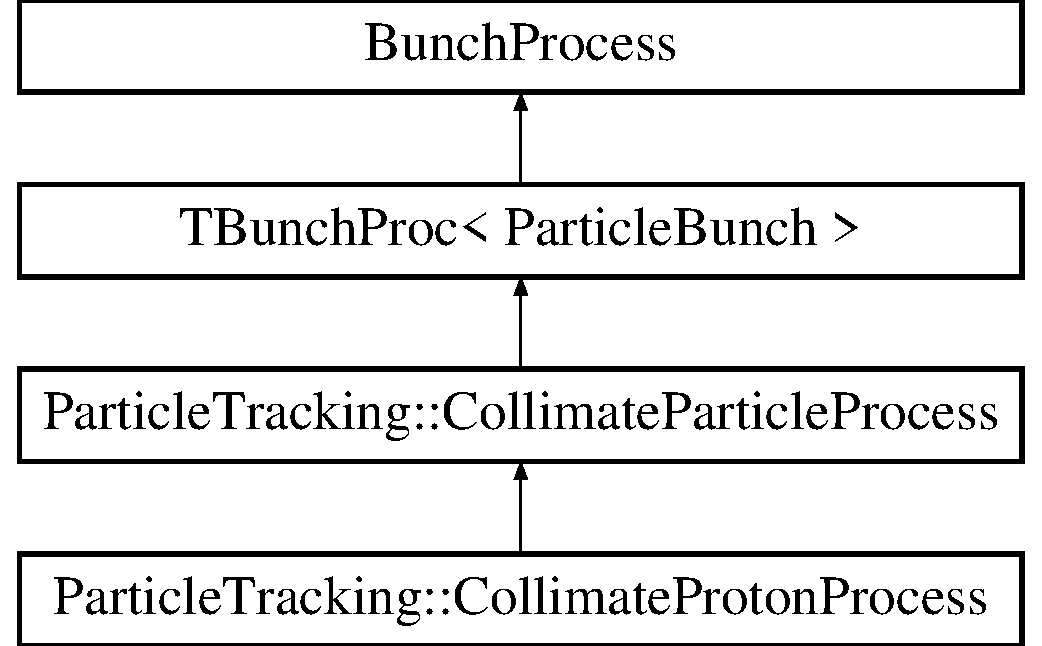
\includegraphics[height=4.000000cm]{classParticleTracking_1_1CollimateProtonProcess}
\end{center}
\end{figure}
\subsection*{Public Member Functions}
\begin{DoxyCompactItemize}
\item 
\hyperlink{classParticleTracking_1_1CollimateProtonProcess_aebcb1f9c086ac8e79e76a8382f37f4c3}{Collimate\+Proton\+Process} (int priority, int mode, std\+::ostream $\ast$osp=nullptr)
\item 
\mbox{\Hypertarget{classParticleTracking_1_1CollimateProtonProcess_a609995f15fbeba015e59c9ce2afba351}\label{classParticleTracking_1_1CollimateProtonProcess_a609995f15fbeba015e59c9ce2afba351}} 
void {\bfseries Set\+Scattering\+Model} (\hyperlink{classCollimation_1_1ScatteringModel}{Collimation\+::\+Scattering\+Model} $\ast$s)
\end{DoxyCompactItemize}
\subsection*{Additional Inherited Members}


\subsection{Constructor \& Destructor Documentation}
\mbox{\Hypertarget{classParticleTracking_1_1CollimateProtonProcess_aebcb1f9c086ac8e79e76a8382f37f4c3}\label{classParticleTracking_1_1CollimateProtonProcess_aebcb1f9c086ac8e79e76a8382f37f4c3}} 
\index{Particle\+Tracking\+::\+Collimate\+Proton\+Process@{Particle\+Tracking\+::\+Collimate\+Proton\+Process}!Collimate\+Proton\+Process@{Collimate\+Proton\+Process}}
\index{Collimate\+Proton\+Process@{Collimate\+Proton\+Process}!Particle\+Tracking\+::\+Collimate\+Proton\+Process@{Particle\+Tracking\+::\+Collimate\+Proton\+Process}}
\subsubsection{\texorpdfstring{Collimate\+Proton\+Process()}{CollimateProtonProcess()}}
{\footnotesize\ttfamily Particle\+Tracking\+::\+Collimate\+Proton\+Process\+::\+Collimate\+Proton\+Process (\begin{DoxyParamCaption}\item[{int}]{priority,  }\item[{int}]{mode,  }\item[{std\+::ostream $\ast$}]{osp = {\ttfamily nullptr} }\end{DoxyParamCaption})}

Constructor taking the collimation mode, and the output stream pointer to which to print the results. mode can be a logical OR combination of the collimation modes. A null pointer for osp (default) suppresses output. 

The documentation for this class was generated from the following files\+:\begin{DoxyCompactItemize}
\item 
/home/fallon/git/merlin-\/cmake/\+Merlin/Collimate\+Proton\+Process.\+h\item 
/home/fallon/git/merlin-\/cmake/\+Merlin/Collimate\+Proton\+Process.\+cpp\end{DoxyCompactItemize}

\hypertarget{classParticleTracking_1_1CollimationOutput}{}\section{Particle\+Tracking\+:\+:Collimation\+Output Class Reference}
\label{classParticleTracking_1_1CollimationOutput}\index{Particle\+Tracking\+::\+Collimation\+Output@{Particle\+Tracking\+::\+Collimation\+Output}}


{\ttfamily \#include $<$Collimation\+Output.\+h$>$}

Inheritance diagram for Particle\+Tracking\+:\+:Collimation\+Output\+:\begin{figure}[H]
\begin{center}
\leavevmode
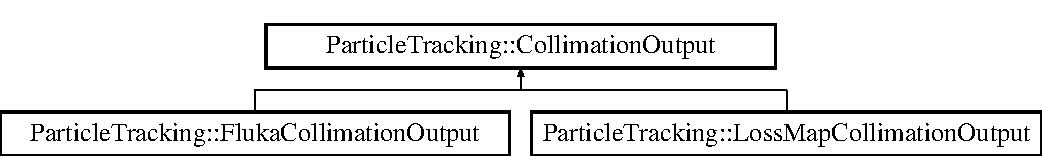
\includegraphics[height=2.000000cm]{classParticleTracking_1_1CollimationOutput}
\end{center}
\end{figure}
\subsection*{Public Member Functions}
\begin{DoxyCompactItemize}
\item 
\mbox{\Hypertarget{classParticleTracking_1_1CollimationOutput_a238ba78a99bc3b19b91b784860fcdc78}\label{classParticleTracking_1_1CollimationOutput_a238ba78a99bc3b19b91b784860fcdc78}} 
{\bfseries Collimation\+Output} (Output\+Type otype=nearestelement)
\item 
\mbox{\Hypertarget{classParticleTracking_1_1CollimationOutput_a7d6306b0c7bedc6a69637955f937c28c}\label{classParticleTracking_1_1CollimationOutput_a7d6306b0c7bedc6a69637955f937c28c}} 
virtual void {\bfseries Finalise} ()
\item 
\mbox{\Hypertarget{classParticleTracking_1_1CollimationOutput_abf969e669e6e55c32c76ea283ad299bf}\label{classParticleTracking_1_1CollimationOutput_abf969e669e6e55c32c76ea283ad299bf}} 
virtual void {\bfseries Output} (std\+::ostream $\ast$os)
\item 
\mbox{\Hypertarget{classParticleTracking_1_1CollimationOutput_a3f6588b17f24390257331804bc2e4280}\label{classParticleTracking_1_1CollimationOutput_a3f6588b17f24390257331804bc2e4280}} 
virtual void {\bfseries Dispose} (\hyperlink{classAcceleratorComponent}{Accelerator\+Component} \&currcomponent, double pos, \hyperlink{classPSvector}{Particle} \&particle, int turn=0)
\end{DoxyCompactItemize}
\subsection*{Public Attributes}
\begin{DoxyCompactItemize}
\item 
\mbox{\Hypertarget{classParticleTracking_1_1CollimationOutput_a93800f83f3cb5f670f8be5f3d81ade41}\label{classParticleTracking_1_1CollimationOutput_a93800f83f3cb5f670f8be5f3d81ade41}} 
Output\+Type {\bfseries otype}
\item 
\mbox{\Hypertarget{classParticleTracking_1_1CollimationOutput_a5862c5673daf1373dedd1c08a76692ee}\label{classParticleTracking_1_1CollimationOutput_a5862c5673daf1373dedd1c08a76692ee}} 
\hyperlink{structParticleTracking_1_1LossData}{Loss\+Data} {\bfseries temp}
\item 
\mbox{\Hypertarget{classParticleTracking_1_1CollimationOutput_a1f881bfef9b1a6eda0a804be14ae8d70}\label{classParticleTracking_1_1CollimationOutput_a1f881bfef9b1a6eda0a804be14ae8d70}} 
std\+::vector$<$ \hyperlink{structParticleTracking_1_1LossData}{Loss\+Data} $>$ {\bfseries Dead\+Particles}
\item 
\mbox{\Hypertarget{classParticleTracking_1_1CollimationOutput_af373054ef09844f2926ab59c0d3a8be5}\label{classParticleTracking_1_1CollimationOutput_af373054ef09844f2926ab59c0d3a8be5}} 
std\+::vector$<$ \hyperlink{structParticleTracking_1_1LossData}{Loss\+Data} $>$ {\bfseries Output\+Losses}
\end{DoxyCompactItemize}
\subsection*{Protected Attributes}
\begin{DoxyCompactItemize}
\item 
\mbox{\Hypertarget{classParticleTracking_1_1CollimationOutput_aa592d3da5fe8ffe8abc05b1e473b92d6}\label{classParticleTracking_1_1CollimationOutput_aa592d3da5fe8ffe8abc05b1e473b92d6}} 
\hyperlink{classAcceleratorComponent}{Accelerator\+Component} $\ast$ {\bfseries current\+Component}
\end{DoxyCompactItemize}


\subsection{Detailed Description}
\hyperlink{classParticleTracking_1_1CollimationOutput}{Collimation\+Output} handles the output from the collimation process, specifically lost particles. It is called from Collimate\+Proton\+Process\+::\+Do\+Scatter and allows the user to create loss map output files, root hist files, or a user specified output format. 

The documentation for this class was generated from the following files\+:\begin{DoxyCompactItemize}
\item 
/home/fallon/git/merlin-\/cmake/\+Merlin/Collimation\+Output.\+h\item 
/home/fallon/git/merlin-\/cmake/\+Merlin/Collimation\+Output.\+cpp\end{DoxyCompactItemize}

\hypertarget{classCollimator}{}\section{Collimator Class Reference}
\label{classCollimator}\index{Collimator@{Collimator}}
Inheritance diagram for Collimator\+:\begin{figure}[H]
\begin{center}
\leavevmode
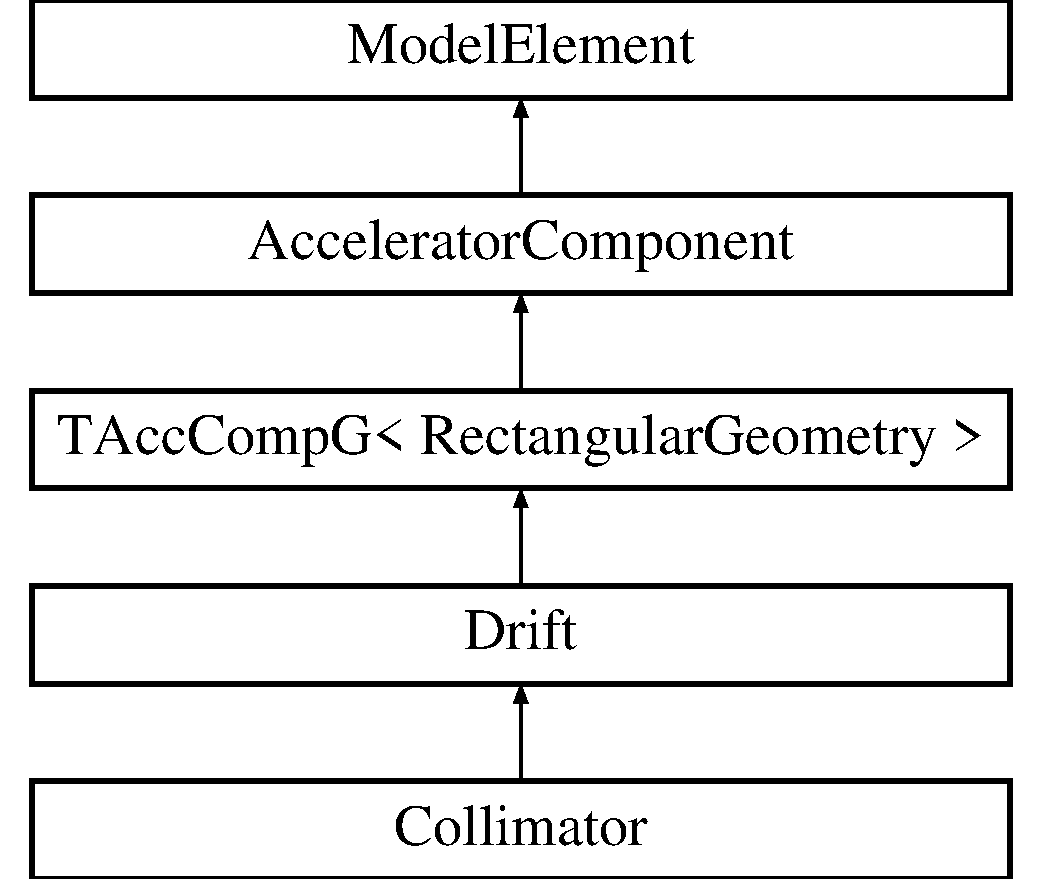
\includegraphics[height=5.000000cm]{classCollimator}
\end{center}
\end{figure}
\subsection*{Public Member Functions}
\begin{DoxyCompactItemize}
\item 
\mbox{\Hypertarget{classCollimator_ab48a84c675c70f019d22135d487c2196}\label{classCollimator_ab48a84c675c70f019d22135d487c2196}} 
{\bfseries Collimator} (const string \&\hyperlink{classModelElement_aada171ead2085c75b592cf07d91bc5c2}{id}, double len)
\item 
\mbox{\Hypertarget{classCollimator_ad2ccfcac873485325e5d3ab81d6074bc}\label{classCollimator_ad2ccfcac873485325e5d3ab81d6074bc}} 
{\bfseries Collimator} (const string \&\hyperlink{classModelElement_aada171ead2085c75b592cf07d91bc5c2}{id}, double len, double rad\+Length)
\item 
\mbox{\Hypertarget{classCollimator_a62fb8545803efcdfe2ec6e4148efe56b}\label{classCollimator_a62fb8545803efcdfe2ec6e4148efe56b}} 
{\bfseries Collimator} (const string \&\hyperlink{classModelElement_aada171ead2085c75b592cf07d91bc5c2}{id}, double len, \hyperlink{classMaterial}{Material} $\ast$pp, double P0)
\item 
\mbox{\Hypertarget{classCollimator_a5ee805434a47d85f881fd34bf659c4c5}\label{classCollimator_a5ee805434a47d85f881fd34bf659c4c5}} 
double {\bfseries Get\+Num\+Rad\+Lengths} () const
\item 
\mbox{\Hypertarget{classCollimator_a7e3d4a833345b797ab162809cc8317bd}\label{classCollimator_a7e3d4a833345b797ab162809cc8317bd}} 
double {\bfseries Get\+Material\+Radiation\+Length} () const
\item 
virtual const string \& \hyperlink{classCollimator_aab811743031565147b965ca9b9fdfbc4}{Get\+Type} () const
\item 
virtual int \hyperlink{classCollimator_a158a9d8999d55a27efe4e56e5af8b56a}{Get\+Index} () const
\item 
virtual void \hyperlink{classCollimator_acbcf691bfcf53d652d14b9381c711fe7}{Prepare\+Tracker} (\hyperlink{classComponentTracker}{Component\+Tracker} \&a\+Tracker)
\item 
virtual void \hyperlink{classCollimator_a89d782779f8e57af28eeb963078bbf20}{Rotate\+Y180} ()
\item 
virtual \hyperlink{classModelElement}{Model\+Element} $\ast$ \hyperlink{classCollimator_a82e63d47e1688d84f2e8f2fc3d247700}{Copy} () const
\item 
\mbox{\Hypertarget{classCollimator_af3b0682b5f87377f653370e38d831edb}\label{classCollimator_af3b0682b5f87377f653370e38d831edb}} 
virtual void {\bfseries Set\+Coll\+ID} (int n)
\item 
\mbox{\Hypertarget{classCollimator_a7efb007cd0aa46b4e15260a983eb3fd4}\label{classCollimator_a7efb007cd0aa46b4e15260a983eb3fd4}} 
virtual int {\bfseries Get\+Coll\+ID} ()
\item 
\mbox{\Hypertarget{classCollimator_a023abea4e74906fd0e2b6d74a7d679b6}\label{classCollimator_a023abea4e74906fd0e2b6d74a7d679b6}} 
virtual void {\bfseries Set\+Material} (\hyperlink{classMaterial}{Material} $\ast$pp)
\end{DoxyCompactItemize}
\subsection*{Public Attributes}
\begin{DoxyCompactItemize}
\item 
\mbox{\Hypertarget{classCollimator_afa138af5a4dc2f3bea288b00ab8daf6c}\label{classCollimator_afa138af5a4dc2f3bea288b00ab8daf6c}} 
bool {\bfseries scatter\+\_\+at\+\_\+this\+\_\+collimator}
\item 
\mbox{\Hypertarget{classCollimator_ac4c4bda4b1e20e8b9a943c168bbaa18b}\label{classCollimator_ac4c4bda4b1e20e8b9a943c168bbaa18b}} 
\hyperlink{classMaterial}{Material} $\ast$ {\bfseries p}
\end{DoxyCompactItemize}
\subsection*{Static Public Attributes}
\begin{DoxyCompactItemize}
\item 
\mbox{\Hypertarget{classCollimator_ac20290ce8e9880c343436e04166c05fb}\label{classCollimator_ac20290ce8e9880c343436e04166c05fb}} 
static const int {\bfseries ID} = \hyperlink{classAcceleratorComponent_aa7ad4d39e1a488b705983842ed1ac784}{Unique\+Index}()
\end{DoxyCompactItemize}
\subsection*{Additional Inherited Members}


\subsection{Member Function Documentation}
\mbox{\Hypertarget{classCollimator_a82e63d47e1688d84f2e8f2fc3d247700}\label{classCollimator_a82e63d47e1688d84f2e8f2fc3d247700}} 
\index{Collimator@{Collimator}!Copy@{Copy}}
\index{Copy@{Copy}!Collimator@{Collimator}}
\subsubsection{\texorpdfstring{Copy()}{Copy()}}
{\footnotesize\ttfamily \hyperlink{classModelElement}{Model\+Element} $\ast$ Collimator\+::\+Copy (\begin{DoxyParamCaption}{ }\end{DoxyParamCaption}) const\hspace{0.3cm}{\ttfamily [virtual]}}

Virtual constructor. 

Reimplemented from \hyperlink{classDrift_ae47df31297596e13944364d602c95ce5}{Drift}.

\mbox{\Hypertarget{classCollimator_a158a9d8999d55a27efe4e56e5af8b56a}\label{classCollimator_a158a9d8999d55a27efe4e56e5af8b56a}} 
\index{Collimator@{Collimator}!Get\+Index@{Get\+Index}}
\index{Get\+Index@{Get\+Index}!Collimator@{Collimator}}
\subsubsection{\texorpdfstring{Get\+Index()}{GetIndex()}}
{\footnotesize\ttfamily int Collimator\+::\+Get\+Index (\begin{DoxyParamCaption}{ }\end{DoxyParamCaption}) const\hspace{0.3cm}{\ttfamily [virtual]}}

Returns the unique index for this class of accelerator components. \begin{DoxyReturn}{Returns}
An integer containing the unique index for this \hyperlink{classAcceleratorComponent}{Accelerator\+Component} type. 
\end{DoxyReturn}


Reimplemented from \hyperlink{classDrift_a19bc19d48348912f8693e3ebbf9e92f2}{Drift}.

\mbox{\Hypertarget{classCollimator_aab811743031565147b965ca9b9fdfbc4}\label{classCollimator_aab811743031565147b965ca9b9fdfbc4}} 
\index{Collimator@{Collimator}!Get\+Type@{Get\+Type}}
\index{Get\+Type@{Get\+Type}!Collimator@{Collimator}}
\subsubsection{\texorpdfstring{Get\+Type()}{GetType()}}
{\footnotesize\ttfamily const string \& Collimator\+::\+Get\+Type (\begin{DoxyParamCaption}{ }\end{DoxyParamCaption}) const\hspace{0.3cm}{\ttfamily [virtual]}}

Return the type string for the element. \begin{DoxyReturn}{Returns}
A string containing the type of the element. 
\end{DoxyReturn}


Reimplemented from \hyperlink{classDrift_a9f5e7d0aafd8689a4420b3d5e7b6879e}{Drift}.

\mbox{\Hypertarget{classCollimator_acbcf691bfcf53d652d14b9381c711fe7}\label{classCollimator_acbcf691bfcf53d652d14b9381c711fe7}} 
\index{Collimator@{Collimator}!Prepare\+Tracker@{Prepare\+Tracker}}
\index{Prepare\+Tracker@{Prepare\+Tracker}!Collimator@{Collimator}}
\subsubsection{\texorpdfstring{Prepare\+Tracker()}{PrepareTracker()}}
{\footnotesize\ttfamily void Collimator\+::\+Prepare\+Tracker (\begin{DoxyParamCaption}\item[{\hyperlink{classComponentTracker}{Component\+Tracker} \&}]{a\+Tracker }\end{DoxyParamCaption})\hspace{0.3cm}{\ttfamily [virtual]}}

Primary tracking interface. Prepares the specified Tracker object for tracking this component. 
\begin{DoxyParams}[1]{Parameters}
\mbox{\tt in,out}  & {\em a\+Tracker} & The tracker to prepare. \\
\hline
\end{DoxyParams}


Reimplemented from \hyperlink{classDrift_a9f3925549a0c7c99b39a1abea8546642}{Drift}.

\mbox{\Hypertarget{classCollimator_a89d782779f8e57af28eeb963078bbf20}\label{classCollimator_a89d782779f8e57af28eeb963078bbf20}} 
\index{Collimator@{Collimator}!Rotate\+Y180@{Rotate\+Y180}}
\index{Rotate\+Y180@{Rotate\+Y180}!Collimator@{Collimator}}
\subsubsection{\texorpdfstring{Rotate\+Y180()}{RotateY180()}}
{\footnotesize\ttfamily void Collimator\+::\+Rotate\+Y180 (\begin{DoxyParamCaption}{ }\end{DoxyParamCaption})\hspace{0.3cm}{\ttfamily [virtual]}}

Rotates the component 180 degrees about its local Y axis. 

Reimplemented from \hyperlink{classDrift_abf387eddfcabfc81b186080f6301ce60}{Drift}.



The documentation for this class was generated from the following files\+:\begin{DoxyCompactItemize}
\item 
/home/fallon/git/merlin-\/cmake/\+Merlin/Collimator.\+h\item 
/home/fallon/git/merlin-\/cmake/\+Merlin/Collimator.\+cpp\end{DoxyCompactItemize}

\hypertarget{classCollimatorAperture}{}\section{Collimator\+Aperture Class Reference}
\label{classCollimatorAperture}\index{Collimator\+Aperture@{Collimator\+Aperture}}
Inheritance diagram for Collimator\+Aperture\+:\begin{figure}[H]
\begin{center}
\leavevmode
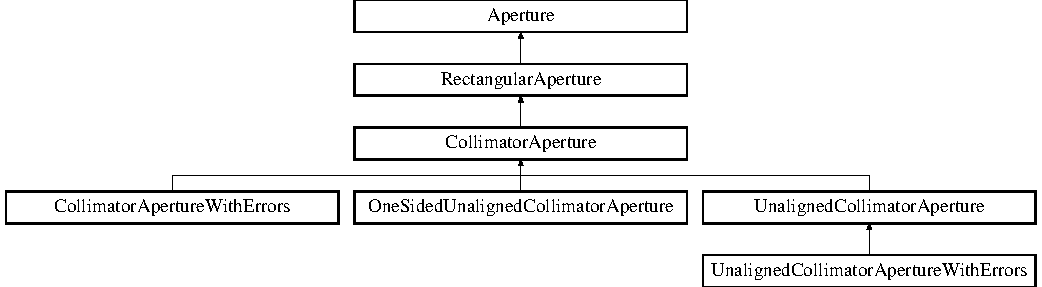
\includegraphics[height=3.856750cm]{classCollimatorAperture}
\end{center}
\end{figure}
\subsection*{Public Member Functions}
\begin{DoxyCompactItemize}
\item 
\mbox{\Hypertarget{classCollimatorAperture_adad8412cd5d214300ff9affba85fd2c0}\label{classCollimatorAperture_adad8412cd5d214300ff9affba85fd2c0}} 
{\bfseries Collimator\+Aperture} (double w, double h, double t, \hyperlink{classMaterial}{Material} $\ast$m, double length, double x\+\_\+offset\+\_\+entry=0.\+0, double y\+\_\+offset\+\_\+entry=0.\+0)
\item 
\mbox{\Hypertarget{classCollimatorAperture_adbb882e5fd5020f445d9434af14c9976}\label{classCollimatorAperture_adbb882e5fd5020f445d9434af14c9976}} 
void {\bfseries Set\+Exit\+Width} (double)
\item 
\mbox{\Hypertarget{classCollimatorAperture_a033019c071c3237758a12426b2271d7c}\label{classCollimatorAperture_a033019c071c3237758a12426b2271d7c}} 
void {\bfseries Set\+Exit\+Height} (double)
\item 
\mbox{\Hypertarget{classCollimatorAperture_a20dc185884657c57576a4429ae252883}\label{classCollimatorAperture_a20dc185884657c57576a4429ae252883}} 
void {\bfseries Set\+Exit\+X\+Offset} (double)
\item 
\mbox{\Hypertarget{classCollimatorAperture_ae36decdc5cf5f485cb49dd2f06560e17}\label{classCollimatorAperture_ae36decdc5cf5f485cb49dd2f06560e17}} 
void {\bfseries Set\+Exit\+Y\+Offset} (double)
\item 
\mbox{\Hypertarget{classCollimatorAperture_afad39797ce9f9b9c2509240cc24b32aa}\label{classCollimatorAperture_afad39797ce9f9b9c2509240cc24b32aa}} 
double {\bfseries Get\+Full\+Entrance\+Height} () const
\item 
\mbox{\Hypertarget{classCollimatorAperture_abb63b6012de92cd33c33cd7b3646830d}\label{classCollimatorAperture_abb63b6012de92cd33c33cd7b3646830d}} 
double {\bfseries Get\+Full\+Entrance\+Width} () const
\item 
\mbox{\Hypertarget{classCollimatorAperture_a3950274bb3219c7a2ac0498446bf6be9}\label{classCollimatorAperture_a3950274bb3219c7a2ac0498446bf6be9}} 
double {\bfseries Get\+Full\+Exit\+Height} () const
\item 
\mbox{\Hypertarget{classCollimatorAperture_a8f0b1847c4fd67a80a638b3b7c052165}\label{classCollimatorAperture_a8f0b1847c4fd67a80a638b3b7c052165}} 
double {\bfseries Get\+Full\+Exit\+Width} () const
\item 
\mbox{\Hypertarget{classCollimatorAperture_ad7c7fb4fb80ce5c7d12a1454ae60d4f2}\label{classCollimatorAperture_ad7c7fb4fb80ce5c7d12a1454ae60d4f2}} 
double {\bfseries Get\+Entrance\+X\+Offset} () const
\item 
\mbox{\Hypertarget{classCollimatorAperture_ac50da50f9ebdaedd28e9af235c039186}\label{classCollimatorAperture_ac50da50f9ebdaedd28e9af235c039186}} 
double {\bfseries Get\+Entrance\+Y\+Offset} () const
\item 
\mbox{\Hypertarget{classCollimatorAperture_a962112540fd88b997ab8019f0ac8c21b}\label{classCollimatorAperture_a962112540fd88b997ab8019f0ac8c21b}} 
double {\bfseries Get\+Exit\+X\+Offset} () const
\item 
\mbox{\Hypertarget{classCollimatorAperture_a871583a668abc5cb83485728a44a2f70}\label{classCollimatorAperture_a871583a668abc5cb83485728a44a2f70}} 
double {\bfseries Get\+Exit\+Y\+Offset} () const
\item 
\mbox{\Hypertarget{classCollimatorAperture_a642ac7c2c581c57e2bb3d817f63c7220}\label{classCollimatorAperture_a642ac7c2c581c57e2bb3d817f63c7220}} 
double {\bfseries Get\+Collimator\+Tilt} () const
\item 
virtual bool \hyperlink{classCollimatorAperture_a964f63287a0ab48900859d75dfa644dc}{Point\+Inside} (double x, double y, double z) const
\end{DoxyCompactItemize}
\subsection*{Protected Attributes}
\begin{DoxyCompactItemize}
\item 
\mbox{\Hypertarget{classCollimatorAperture_a6693e925c07620a86550d68f2684acf1}\label{classCollimatorAperture_a6693e925c07620a86550d68f2684acf1}} 
double {\bfseries alpha}
\item 
\mbox{\Hypertarget{classCollimatorAperture_a0e9a1df31ea6ab02b4097ed94032e112}\label{classCollimatorAperture_a0e9a1df31ea6ab02b4097ed94032e112}} 
double {\bfseries Collimator\+Length}
\item 
\mbox{\Hypertarget{classCollimatorAperture_a9fcd224bf89f803e076ea769412c197d}\label{classCollimatorAperture_a9fcd224bf89f803e076ea769412c197d}} 
double {\bfseries jaw\+\_\+length}
\item 
\mbox{\Hypertarget{classCollimatorAperture_a41ffac3b41d5408b8b545d5c69c36bc3}\label{classCollimatorAperture_a41ffac3b41d5408b8b545d5c69c36bc3}} 
double {\bfseries x\+\_\+offset\+\_\+entry}
\item 
\mbox{\Hypertarget{classCollimatorAperture_a88b7cee0cac55eae2ad0b59344713cfc}\label{classCollimatorAperture_a88b7cee0cac55eae2ad0b59344713cfc}} 
double {\bfseries y\+\_\+offset\+\_\+entry}
\item 
\mbox{\Hypertarget{classCollimatorAperture_af1bf39716a6aa1cb858e73b453b68b44}\label{classCollimatorAperture_af1bf39716a6aa1cb858e73b453b68b44}} 
double {\bfseries x\+\_\+offset\+\_\+exit}
\item 
\mbox{\Hypertarget{classCollimatorAperture_a982d5beff7769e18f0ba0e00931ffda9}\label{classCollimatorAperture_a982d5beff7769e18f0ba0e00931ffda9}} 
double {\bfseries y\+\_\+offset\+\_\+exit}
\item 
\mbox{\Hypertarget{classCollimatorAperture_ac7b2d5e2f7d15a954673121ccf87532e}\label{classCollimatorAperture_ac7b2d5e2f7d15a954673121ccf87532e}} 
double {\bfseries w\+\_\+exit}
\item 
\mbox{\Hypertarget{classCollimatorAperture_a9dbd66e11b024c3b0137a0ac48d9d1f0}\label{classCollimatorAperture_a9dbd66e11b024c3b0137a0ac48d9d1f0}} 
double {\bfseries h\+\_\+exit}
\item 
\mbox{\Hypertarget{classCollimatorAperture_a538827ab2f3b2bc57929bc14dbe883f7}\label{classCollimatorAperture_a538827ab2f3b2bc57929bc14dbe883f7}} 
double {\bfseries cosalpha}
\item 
\mbox{\Hypertarget{classCollimatorAperture_ab4378fb24152e848970c944f82f64af7}\label{classCollimatorAperture_ab4378fb24152e848970c944f82f64af7}} 
double {\bfseries sinalpha}
\end{DoxyCompactItemize}


\subsection{Member Function Documentation}
\mbox{\Hypertarget{classCollimatorAperture_a964f63287a0ab48900859d75dfa644dc}\label{classCollimatorAperture_a964f63287a0ab48900859d75dfa644dc}} 
\index{Collimator\+Aperture@{Collimator\+Aperture}!Point\+Inside@{Point\+Inside}}
\index{Point\+Inside@{Point\+Inside}!Collimator\+Aperture@{Collimator\+Aperture}}
\subsubsection{\texorpdfstring{Point\+Inside()}{PointInside()}}
{\footnotesize\ttfamily bool Collimator\+Aperture\+::\+Point\+Inside (\begin{DoxyParamCaption}\item[{double}]{x,  }\item[{double}]{y,  }\item[{double}]{z }\end{DoxyParamCaption}) const\hspace{0.3cm}{\ttfamily [inline]}, {\ttfamily [virtual]}}

Returns true if the point (x,y,z) is within the aperture. The z coordinate is ignored. 

Reimplemented from \hyperlink{classRectangularAperture_a47e965df14eb63f2a3851ea0e9fe26db}{Rectangular\+Aperture}.



Reimplemented in \hyperlink{classOneSidedUnalignedCollimatorAperture_afad818345b971dffa9ca6fa36a166e35}{One\+Sided\+Unaligned\+Collimator\+Aperture}, and \hyperlink{classUnalignedCollimatorAperture_af116c2ff1d60c4894a9b9ae4cfc2b19e}{Unaligned\+Collimator\+Aperture}.



The documentation for this class was generated from the following files\+:\begin{DoxyCompactItemize}
\item 
/home/fallon/git/merlin-\/cmake/\+Merlin/Collimator\+Aperture.\+h\item 
/home/fallon/git/merlin-\/cmake/\+Merlin/Collimator\+Aperture.\+cpp\end{DoxyCompactItemize}

\hypertarget{classCollimatorApertureWithErrors}{}\section{Collimator\+Aperture\+With\+Errors Class Reference}
\label{classCollimatorApertureWithErrors}\index{Collimator\+Aperture\+With\+Errors@{Collimator\+Aperture\+With\+Errors}}
Inheritance diagram for Collimator\+Aperture\+With\+Errors\+:\begin{figure}[H]
\begin{center}
\leavevmode
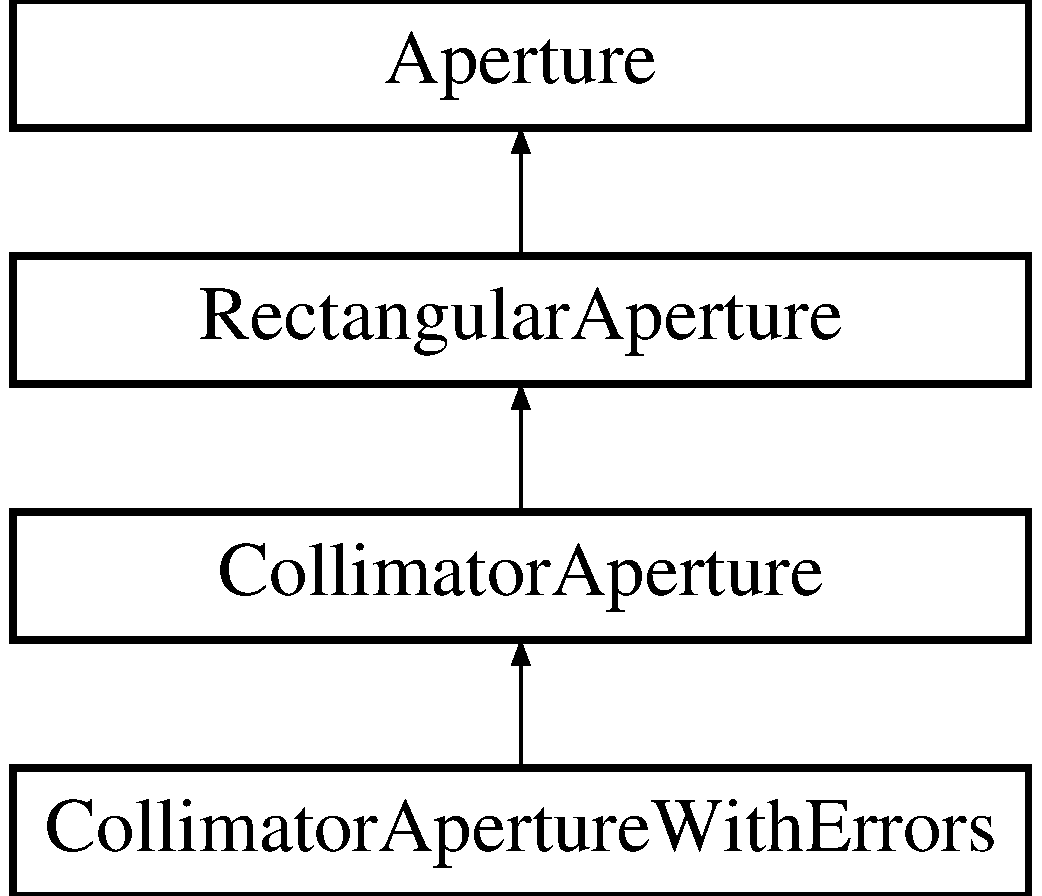
\includegraphics[height=4.000000cm]{classCollimatorApertureWithErrors}
\end{center}
\end{figure}
\subsection*{Additional Inherited Members}


The documentation for this class was generated from the following files\+:\begin{DoxyCompactItemize}
\item 
/home/fallon/git/merlin-\/cmake/\+Merlin/Collimator\+Aperture.\+h\item 
/home/fallon/git/merlin-\/cmake/\+Merlin/Collimator\+Aperture.\+cpp\end{DoxyCompactItemize}

\hypertarget{structCollimatorDatabase_1_1CollimatorData}{}\section{Collimator\+Database\+:\+:Collimator\+Data Struct Reference}
\label{structCollimatorDatabase_1_1CollimatorData}\index{Collimator\+Database\+::\+Collimator\+Data@{Collimator\+Database\+::\+Collimator\+Data}}
\subsection*{Public Attributes}
\begin{DoxyCompactItemize}
\item 
\mbox{\Hypertarget{structCollimatorDatabase_1_1CollimatorData_a1ed6a77cd58187aaf0ea722389f38f19}\label{structCollimatorDatabase_1_1CollimatorData_a1ed6a77cd58187aaf0ea722389f38f19}} 
string {\bfseries name}
\item 
\mbox{\Hypertarget{structCollimatorDatabase_1_1CollimatorData_a5dc32c87ee52ab8fa3ee1621043fe934}\label{structCollimatorDatabase_1_1CollimatorData_a5dc32c87ee52ab8fa3ee1621043fe934}} 
double {\bfseries x\+\_\+gap}
\item 
\mbox{\Hypertarget{structCollimatorDatabase_1_1CollimatorData_ad4fd54532c669c3f6526dc2722d4b56a}\label{structCollimatorDatabase_1_1CollimatorData_ad4fd54532c669c3f6526dc2722d4b56a}} 
double {\bfseries y\+\_\+gap}
\item 
\mbox{\Hypertarget{structCollimatorDatabase_1_1CollimatorData_a898c54733e84d0e3ac8616b9fe9ff0c4}\label{structCollimatorDatabase_1_1CollimatorData_a898c54733e84d0e3ac8616b9fe9ff0c4}} 
double {\bfseries tilt}
\item 
\mbox{\Hypertarget{structCollimatorDatabase_1_1CollimatorData_a54c7282e9c967ecfc2ecc65383951146}\label{structCollimatorDatabase_1_1CollimatorData_a54c7282e9c967ecfc2ecc65383951146}} 
double {\bfseries x\+\_\+offset}
\item 
\mbox{\Hypertarget{structCollimatorDatabase_1_1CollimatorData_a0bd7b9c424b96f27afa177b86fb88495}\label{structCollimatorDatabase_1_1CollimatorData_a0bd7b9c424b96f27afa177b86fb88495}} 
double {\bfseries y\+\_\+offset}
\item 
\mbox{\Hypertarget{structCollimatorDatabase_1_1CollimatorData_a3be4209575cfb2a1007fc6032ab23c43}\label{structCollimatorDatabase_1_1CollimatorData_a3be4209575cfb2a1007fc6032ab23c43}} 
double {\bfseries j1\+\_\+tilt}
\item 
\mbox{\Hypertarget{structCollimatorDatabase_1_1CollimatorData_a6daad4f0f91d9c8c9de32bccde4d115d}\label{structCollimatorDatabase_1_1CollimatorData_a6daad4f0f91d9c8c9de32bccde4d115d}} 
double {\bfseries j2\+\_\+tilt}
\item 
\mbox{\Hypertarget{structCollimatorDatabase_1_1CollimatorData_a7441d0943e80f9bcbdd6f8458aa48a69}\label{structCollimatorDatabase_1_1CollimatorData_a7441d0943e80f9bcbdd6f8458aa48a69}} 
double {\bfseries length}
\item 
\mbox{\Hypertarget{structCollimatorDatabase_1_1CollimatorData_acdf1a13ef311bae190b2c5ed0250bc21}\label{structCollimatorDatabase_1_1CollimatorData_acdf1a13ef311bae190b2c5ed0250bc21}} 
\hyperlink{classMaterial}{Material} $\ast$ {\bfseries Jaw\+Material}
\item 
\mbox{\Hypertarget{structCollimatorDatabase_1_1CollimatorData_a93cb9999ca10e8468a5de64245ca2261}\label{structCollimatorDatabase_1_1CollimatorData_a93cb9999ca10e8468a5de64245ca2261}} 
double {\bfseries sigma\+\_\+x}
\item 
\mbox{\Hypertarget{structCollimatorDatabase_1_1CollimatorData_a8820fb77370721e18a13b3d0f4d9a5d9}\label{structCollimatorDatabase_1_1CollimatorData_a8820fb77370721e18a13b3d0f4d9a5d9}} 
double {\bfseries sigma\+\_\+y}
\item 
\mbox{\Hypertarget{structCollimatorDatabase_1_1CollimatorData_a4073c006110a6071fb00811b2c540c1a}\label{structCollimatorDatabase_1_1CollimatorData_a4073c006110a6071fb00811b2c540c1a}} 
double {\bfseries beta\+\_\+x}
\item 
\mbox{\Hypertarget{structCollimatorDatabase_1_1CollimatorData_a7fa27fa0751dd0208a1464cdb99c1cf5}\label{structCollimatorDatabase_1_1CollimatorData_a7fa27fa0751dd0208a1464cdb99c1cf5}} 
double {\bfseries beta\+\_\+y}
\item 
\mbox{\Hypertarget{structCollimatorDatabase_1_1CollimatorData_a1e8877202df1772d054480e0e65a75c4}\label{structCollimatorDatabase_1_1CollimatorData_a1e8877202df1772d054480e0e65a75c4}} 
double {\bfseries position}
\end{DoxyCompactItemize}


The documentation for this struct was generated from the following file\+:\begin{DoxyCompactItemize}
\item 
/home/fallon/git/merlin-\/cmake/\+Merlin/Collimator\+Database.\+h\end{DoxyCompactItemize}

\hypertarget{classCollimatorDatabase}{}\section{Collimator\+Database Class Reference}
\label{classCollimatorDatabase}\index{Collimator\+Database@{Collimator\+Database}}
\subsection*{Classes}
\begin{DoxyCompactItemize}
\item 
struct \hyperlink{structCollimatorDatabase_1_1CollimatorData}{Collimator\+Data}
\item 
struct \hyperlink{structCollimatorDatabase_1_1FlukaData}{Fluka\+Data}
\end{DoxyCompactItemize}
\subsection*{Public Member Functions}
\begin{DoxyCompactItemize}
\item 
\mbox{\Hypertarget{classCollimatorDatabase_a522d3f54bdfcff69de497b91ea8c062b}\label{classCollimatorDatabase_a522d3f54bdfcff69de497b91ea8c062b}} 
{\bfseries Collimator\+Database} (string, \hyperlink{classMaterialDatabase}{Material\+Database} $\ast$, bool use\+\_\+sigma)
\item 
\mbox{\Hypertarget{classCollimatorDatabase_a79ae3c3797a924c0275bcf0d01233f24}\label{classCollimatorDatabase_a79ae3c3797a924c0275bcf0d01233f24}} 
double {\bfseries Configure\+Collimators} (\hyperlink{classAcceleratorModel}{Accelerator\+Model} $\ast$model, double emittance\+\_\+x, double emittance\+\_\+y, \hyperlink{classLatticeFunctionTable}{Lattice\+Function\+Table} $\ast$twiss)
\item 
\mbox{\Hypertarget{classCollimatorDatabase_a7586e2ed55ceb3f6629a1c238139bfd5}\label{classCollimatorDatabase_a7586e2ed55ceb3f6629a1c238139bfd5}} 
void {\bfseries Configure\+Collimators} (\hyperlink{classAcceleratorModel}{Accelerator\+Model} $\ast$model)
\item 
\mbox{\Hypertarget{classCollimatorDatabase_a3148664be49eb8d4b769b6dacbdaa8fd}\label{classCollimatorDatabase_a3148664be49eb8d4b769b6dacbdaa8fd}} 
void {\bfseries Select\+Impact\+Factor} (string pcoll, double impact)
\item 
\mbox{\Hypertarget{classCollimatorDatabase_a1f5c7ad93b128be19abe75f644b799aa}\label{classCollimatorDatabase_a1f5c7ad93b128be19abe75f644b799aa}} 
void {\bfseries Set\+Log\+File} (ostream \&os)
\item 
\mbox{\Hypertarget{classCollimatorDatabase_ac026ba83eb7f7cca7803b83db35a13a8}\label{classCollimatorDatabase_ac026ba83eb7f7cca7803b83db35a13a8}} 
void {\bfseries Enable\+Logging} (bool)
\item 
\mbox{\Hypertarget{classCollimatorDatabase_aa0edd5394c70ac34799e938b45c74ca1}\label{classCollimatorDatabase_aa0edd5394c70ac34799e938b45c74ca1}} 
void {\bfseries Set\+Error\+Log\+File} (ostream \&os)
\item 
\mbox{\Hypertarget{classCollimatorDatabase_a92c66e0b048558a6dcd1c238f5c4c51d}\label{classCollimatorDatabase_a92c66e0b048558a6dcd1c238f5c4c51d}} 
void {\bfseries Enable\+Error\+Logging} (bool)
\item 
\mbox{\Hypertarget{classCollimatorDatabase_aff58a2e845593716bc6142c56a7839db}\label{classCollimatorDatabase_aff58a2e845593716bc6142c56a7839db}} 
void {\bfseries Match\+Beam\+Envelope} (bool)
\item 
\mbox{\Hypertarget{classCollimatorDatabase_a49489d25f279c54fd72e3825366c8679}\label{classCollimatorDatabase_a49489d25f279c54fd72e3825366c8679}} 
void {\bfseries Match\+Reference\+Orbit} (bool)
\item 
\mbox{\Hypertarget{classCollimatorDatabase_a4f0344dfcf085122ef6d3c86100b9d38}\label{classCollimatorDatabase_a4f0344dfcf085122ef6d3c86100b9d38}} 
void {\bfseries Enable\+Jaw\+Flattness\+Errors} (bool)
\item 
\mbox{\Hypertarget{classCollimatorDatabase_aebc1598dbf4c8f17bc492f76c088bd4c}\label{classCollimatorDatabase_aebc1598dbf4c8f17bc492f76c088bd4c}} 
void {\bfseries Enable\+Jaw\+Alignment\+Errors} (bool)
\item 
\mbox{\Hypertarget{classCollimatorDatabase_a3bef02a7762d782bfb3ed381524f2545}\label{classCollimatorDatabase_a3bef02a7762d782bfb3ed381524f2545}} 
void {\bfseries Set\+Jaw\+Position\+Error} (double)
\item 
\mbox{\Hypertarget{classCollimatorDatabase_a7b0a6de72a3e3a1ce4b5b707555962fb}\label{classCollimatorDatabase_a7b0a6de72a3e3a1ce4b5b707555962fb}} 
void {\bfseries Set\+Jaw\+Angle\+Error} (double)
\item 
\mbox{\Hypertarget{classCollimatorDatabase_ada524dc893dd45c13589f056d3f88395}\label{classCollimatorDatabase_ada524dc893dd45c13589f056d3f88395}} 
void {\bfseries Output\+Fluka\+Database} (std\+::ostream $\ast$os)
\end{DoxyCompactItemize}
\subsection*{Public Attributes}
\begin{DoxyCompactItemize}
\item 
\mbox{\Hypertarget{classCollimatorDatabase_a9b40299413a16a35cfe70c84bb84b2c6}\label{classCollimatorDatabase_a9b40299413a16a35cfe70c84bb84b2c6}} 
\hyperlink{structCollimatorDatabase_1_1CollimatorData}{Collimator\+Data} $\ast$ {\bfseries Coll\+Data}
\item 
\mbox{\Hypertarget{classCollimatorDatabase_af76c72a800ad72332d2b8e419e61cf02}\label{classCollimatorDatabase_af76c72a800ad72332d2b8e419e61cf02}} 
size\+\_\+t {\bfseries number\+\_\+collimators}
\item 
\mbox{\Hypertarget{classCollimatorDatabase_a365430d78ff5805a7bddae31881a2344}\label{classCollimatorDatabase_a365430d78ff5805a7bddae31881a2344}} 
bool {\bfseries use\+\_\+sigma}
\item 
\mbox{\Hypertarget{classCollimatorDatabase_a11105d827fb57a9f8a6bcbb5516f5851}\label{classCollimatorDatabase_a11105d827fb57a9f8a6bcbb5516f5851}} 
vector$<$ \hyperlink{structCollimatorDatabase_1_1FlukaData}{Fluka\+Data} $\ast$ $>$ {\bfseries Stored\+Fluka\+Data}
\end{DoxyCompactItemize}
\subsection*{Protected Attributes}
\begin{DoxyCompactItemize}
\item 
\mbox{\Hypertarget{classCollimatorDatabase_a7b8b2127314a0b01855807e5e5a2963b}\label{classCollimatorDatabase_a7b8b2127314a0b01855807e5e5a2963b}} 
string {\bfseries Primary\+Collimator}
\item 
\mbox{\Hypertarget{classCollimatorDatabase_ad25fe80be4cc702d137d68340a0a5ad5}\label{classCollimatorDatabase_ad25fe80be4cc702d137d68340a0a5ad5}} 
double {\bfseries Requested\+Impact\+Factor}
\item 
\mbox{\Hypertarget{classCollimatorDatabase_a2c655e155d1de5d24c2c4084f4e51949}\label{classCollimatorDatabase_a2c655e155d1de5d24c2c4084f4e51949}} 
double {\bfseries Impact\+Sigma}
\item 
\mbox{\Hypertarget{classCollimatorDatabase_acbeb55e323d44910f2c1f5b234bf9e34}\label{classCollimatorDatabase_acbeb55e323d44910f2c1f5b234bf9e34}} 
ostream $\ast$ {\bfseries log}
\item 
\mbox{\Hypertarget{classCollimatorDatabase_ac792ee7809133d779463e04ba74722cb}\label{classCollimatorDatabase_ac792ee7809133d779463e04ba74722cb}} 
bool {\bfseries log\+Flag}
\item 
\mbox{\Hypertarget{classCollimatorDatabase_afd80ffc3255c28d3699561ee6a2415f2}\label{classCollimatorDatabase_afd80ffc3255c28d3699561ee6a2415f2}} 
ostream $\ast$ {\bfseries Error\+Log}
\item 
\mbox{\Hypertarget{classCollimatorDatabase_a416745423609e03c2ef3eb65210a559d}\label{classCollimatorDatabase_a416745423609e03c2ef3eb65210a559d}} 
bool {\bfseries Error\+Log\+Flag}
\item 
\mbox{\Hypertarget{classCollimatorDatabase_a9c773f7d9140ae71b1dc7fe4b4931120}\label{classCollimatorDatabase_a9c773f7d9140ae71b1dc7fe4b4931120}} 
bool {\bfseries One\+Side\+Jaw\+T\+C\+D\+QA}
\item 
\mbox{\Hypertarget{classCollimatorDatabase_a667e972952d2417741699b9bd6b1cf10}\label{classCollimatorDatabase_a667e972952d2417741699b9bd6b1cf10}} 
bool {\bfseries Enable\+Match\+Beam\+Envelope}
\item 
\mbox{\Hypertarget{classCollimatorDatabase_a62909c92e8ec2fc1b9cd4b1662484006}\label{classCollimatorDatabase_a62909c92e8ec2fc1b9cd4b1662484006}} 
bool {\bfseries Enable\+Match\+Reference\+Orbit}
\item 
\mbox{\Hypertarget{classCollimatorDatabase_ada2dff3b62ee40ad440b49a031c69cea}\label{classCollimatorDatabase_ada2dff3b62ee40ad440b49a031c69cea}} 
bool {\bfseries Jaw\+Flattness\+Errors}
\item 
\mbox{\Hypertarget{classCollimatorDatabase_a56e1b47ff877e1cbbff3bcdc62e587a9}\label{classCollimatorDatabase_a56e1b47ff877e1cbbff3bcdc62e587a9}} 
bool {\bfseries Jaw\+Alignment\+Errors}
\item 
\mbox{\Hypertarget{classCollimatorDatabase_af4a5410c7927aaaeed7b1cd323010670}\label{classCollimatorDatabase_af4a5410c7927aaaeed7b1cd323010670}} 
bool {\bfseries Enable\+Resistive\+Collimator\+Wakes}
\item 
\mbox{\Hypertarget{classCollimatorDatabase_ab3bc7c834c40288b5998799a25274457}\label{classCollimatorDatabase_ab3bc7c834c40288b5998799a25274457}} 
double {\bfseries Angle\+Error}
\item 
\mbox{\Hypertarget{classCollimatorDatabase_a1d6fa3b40d99e448b4acb99b8e792673}\label{classCollimatorDatabase_a1d6fa3b40d99e448b4acb99b8e792673}} 
double {\bfseries Position\+Error}
\end{DoxyCompactItemize}


The documentation for this class was generated from the following files\+:\begin{DoxyCompactItemize}
\item 
/home/fallon/git/merlin-\/cmake/\+Merlin/Collimator\+Database.\+h\item 
/home/fallon/git/merlin-\/cmake/\+Merlin/Collimator\+Database.\+cpp\end{DoxyCompactItemize}

\hypertarget{classcollimatortable}{}\section{collimatortable Class Reference}
\label{classcollimatortable}\index{collimatortable@{collimatortable}}
\subsection*{Public Member Functions}
\begin{DoxyCompactItemize}
\item 
\mbox{\Hypertarget{classcollimatortable_a643ad3aa5ed1fc9b40f1cdb2a72ee235}\label{classcollimatortable_a643ad3aa5ed1fc9b40f1cdb2a72ee235}} 
bool {\bfseries inrange} (double x)
\item 
\mbox{\Hypertarget{classcollimatortable_a7c5f7dc44d2a1edb34a457bc0a19f171}\label{classcollimatortable_a7c5f7dc44d2a1edb34a457bc0a19f171}} 
double {\bfseries parabolic} (double v1, double v2, double v3, double d)
\item 
\mbox{\Hypertarget{classcollimatortable_a185fb12140e882bc6d5a49359d51924d}\label{classcollimatortable_a185fb12140e882bc6d5a49359d51924d}} 
double {\bfseries interpolate} (double s)
\item 
\mbox{\Hypertarget{classcollimatortable_a80bc57031c95f6923894879dc0a90660}\label{classcollimatortable_a80bc57031c95f6923894879dc0a90660}} 
{\bfseries collimatortable} (const char $\ast$file, double Gamma=0, double xi=0)
\end{DoxyCompactItemize}


The documentation for this class was generated from the following file\+:\begin{DoxyCompactItemize}
\item 
/home/fallon/git/merlin-\/cmake/\+Merlin/Collimator\+Table.\+h\end{DoxyCompactItemize}

\hypertarget{classCollimatorWakePotentials}{}\section{Collimator\+Wake\+Potentials Class Reference}
\label{classCollimatorWakePotentials}\index{Collimator\+Wake\+Potentials@{Collimator\+Wake\+Potentials}}


{\ttfamily \#include $<$Collimator\+Wake\+Potentials.\+h$>$}

Inheritance diagram for Collimator\+Wake\+Potentials\+:\begin{figure}[H]
\begin{center}
\leavevmode
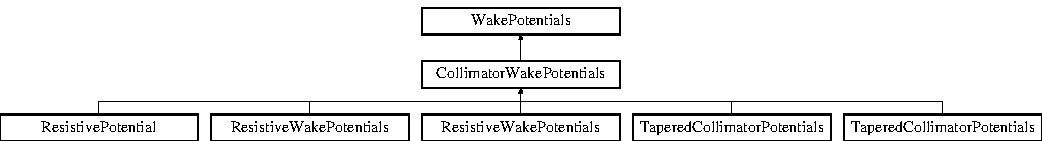
\includegraphics[height=1.898305cm]{classCollimatorWakePotentials}
\end{center}
\end{figure}
\subsection*{Public Member Functions}
\begin{DoxyCompactItemize}
\item 
\mbox{\Hypertarget{classCollimatorWakePotentials_ab22c8d82e26094888578038b9038edc4}\label{classCollimatorWakePotentials_ab22c8d82e26094888578038b9038edc4}} 
{\bfseries Collimator\+Wake\+Potentials} (int m, double rad=0, double conduct=0)
\item 
\mbox{\Hypertarget{classCollimatorWakePotentials_a9bb8993b24d511ef41d43c7273b232da}\label{classCollimatorWakePotentials_a9bb8993b24d511ef41d43c7273b232da}} 
virtual double {\bfseries Wlong} (double s, int m) const =0
\item 
\mbox{\Hypertarget{classCollimatorWakePotentials_a2c1dd7c28101b8fbe26b6dcf889ddeaa}\label{classCollimatorWakePotentials_a2c1dd7c28101b8fbe26b6dcf889ddeaa}} 
virtual double {\bfseries Wtrans} (double s, int m) const =0
\end{DoxyCompactItemize}
\subsection*{Protected Attributes}
\begin{DoxyCompactItemize}
\item 
\mbox{\Hypertarget{classCollimatorWakePotentials_a1286185550a00371317d394f65c23d48}\label{classCollimatorWakePotentials_a1286185550a00371317d394f65c23d48}} 
int {\bfseries nmodes}
\end{DoxyCompactItemize}


\subsection{Detailed Description}
Abstract class for calculating the longitudinal and transverse single-\/bunch wakefield potentials (Greens functions) with modes 

The documentation for this class was generated from the following file\+:\begin{DoxyCompactItemize}
\item 
/home/fallon/git/merlin-\/cmake/\+Merlin/Collimator\+Wake\+Potentials.\+h\end{DoxyCompactItemize}

\hypertarget{classParticleTracking_1_1CollimatorWakeProcess}{}\section{Particle\+Tracking\+:\+:Collimator\+Wake\+Process Class Reference}
\label{classParticleTracking_1_1CollimatorWakeProcess}\index{Particle\+Tracking\+::\+Collimator\+Wake\+Process@{Particle\+Tracking\+::\+Collimator\+Wake\+Process}}


{\ttfamily \#include $<$Collimator\+Wake\+Process.\+h$>$}

Inheritance diagram for Particle\+Tracking\+:\+:Collimator\+Wake\+Process\+:\begin{figure}[H]
\begin{center}
\leavevmode
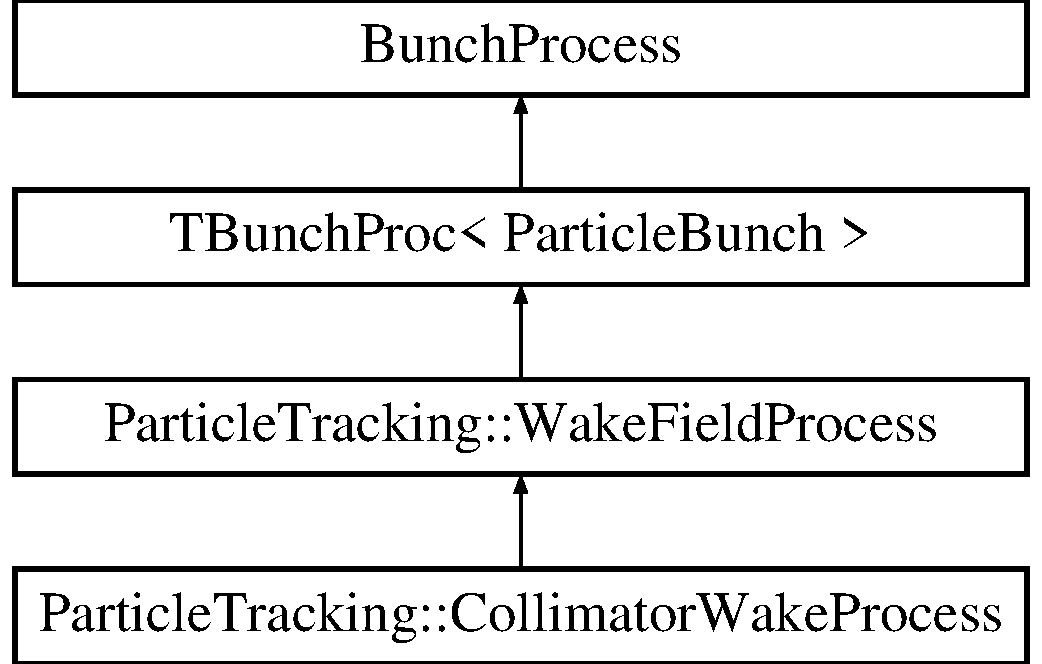
\includegraphics[height=4.000000cm]{classParticleTracking_1_1CollimatorWakeProcess}
\end{center}
\end{figure}
\subsection*{Public Member Functions}
\begin{DoxyCompactItemize}
\item 
\mbox{\Hypertarget{classParticleTracking_1_1CollimatorWakeProcess_a1687e6bd771ce5e53248951e5a9594a7}\label{classParticleTracking_1_1CollimatorWakeProcess_a1687e6bd771ce5e53248951e5a9594a7}} 
{\bfseries Collimator\+Wake\+Process} (int, int, size\+\_\+t, double)
\item 
\mbox{\Hypertarget{classParticleTracking_1_1CollimatorWakeProcess_a7506091d0d9a7c42a197e9d5142e7d7e}\label{classParticleTracking_1_1CollimatorWakeProcess_a7506091d0d9a7c42a197e9d5142e7d7e}} 
virtual void {\bfseries Apply\+Wakefield} (double)
\item 
\mbox{\Hypertarget{classParticleTracking_1_1CollimatorWakeProcess_a9e82c6f3737bb7a27f9ed008494d7d83}\label{classParticleTracking_1_1CollimatorWakeProcess_a9e82c6f3737bb7a27f9ed008494d7d83}} 
virtual void {\bfseries Calculate\+WakeT} (double, int)
\item 
\mbox{\Hypertarget{classParticleTracking_1_1CollimatorWakeProcess_ac2d3d936f632db178288b64877e08231}\label{classParticleTracking_1_1CollimatorWakeProcess_ac2d3d936f632db178288b64877e08231}} 
virtual void {\bfseries Calculate\+WakeL} (double, int)
\end{DoxyCompactItemize}
\subsection*{Additional Inherited Members}


\subsection{Detailed Description}
Class for calculating the longitudinal and transverse single-\/bunch wakefields for Collimators with modes 

The documentation for this class was generated from the following files\+:\begin{DoxyCompactItemize}
\item 
/home/fallon/git/merlin-\/cmake/\+Merlin/Collimator\+Wake\+Process.\+h\item 
/home/fallon/git/merlin-\/cmake/\+Merlin/Collimator\+Wake\+Process.\+cpp\end{DoxyCompactItemize}

\hypertarget{structParticleTracking_1_1SYMPLECTIC_1_1CombinedFunctionSectorBendMap}{}\section{Particle\+Tracking\+:\+:S\+Y\+M\+P\+L\+E\+C\+T\+IC\+:\+:Combined\+Function\+Sector\+Bend\+Map Struct Reference}
\label{structParticleTracking_1_1SYMPLECTIC_1_1CombinedFunctionSectorBendMap}\index{Particle\+Tracking\+::\+S\+Y\+M\+P\+L\+E\+C\+T\+I\+C\+::\+Combined\+Function\+Sector\+Bend\+Map@{Particle\+Tracking\+::\+S\+Y\+M\+P\+L\+E\+C\+T\+I\+C\+::\+Combined\+Function\+Sector\+Bend\+Map}}
\subsection*{Public Member Functions}
\begin{DoxyCompactItemize}
\item 
\mbox{\Hypertarget{structParticleTracking_1_1SYMPLECTIC_1_1CombinedFunctionSectorBendMap_a70f052af5ba4063ebbb54c2fc254171f}\label{structParticleTracking_1_1SYMPLECTIC_1_1CombinedFunctionSectorBendMap_a70f052af5ba4063ebbb54c2fc254171f}} 
{\bfseries Combined\+Function\+Sector\+Bend\+Map} (double \+\_\+h, double \+\_\+k1, double \+\_\+ds)
\item 
\mbox{\Hypertarget{structParticleTracking_1_1SYMPLECTIC_1_1CombinedFunctionSectorBendMap_aff39718739fdc8fd508b1dcf238e8031}\label{structParticleTracking_1_1SYMPLECTIC_1_1CombinedFunctionSectorBendMap_aff39718739fdc8fd508b1dcf238e8031}} 
void {\bfseries operator()} (\hyperlink{classPSvector}{P\+Svector} \&v) const
\end{DoxyCompactItemize}


The documentation for this struct was generated from the following file\+:\begin{DoxyCompactItemize}
\item 
/home/fallon/git/merlin-\/cmake/\+Merlin/Symplectic\+Integrators.\+cpp\end{DoxyCompactItemize}

\hypertarget{classCombinedWakeRF}{}\section{Combined\+Wake\+RF Class Reference}
\label{classCombinedWakeRF}\index{Combined\+Wake\+RF@{Combined\+Wake\+RF}}
Inheritance diagram for Combined\+Wake\+RF\+:\begin{figure}[H]
\begin{center}
\leavevmode
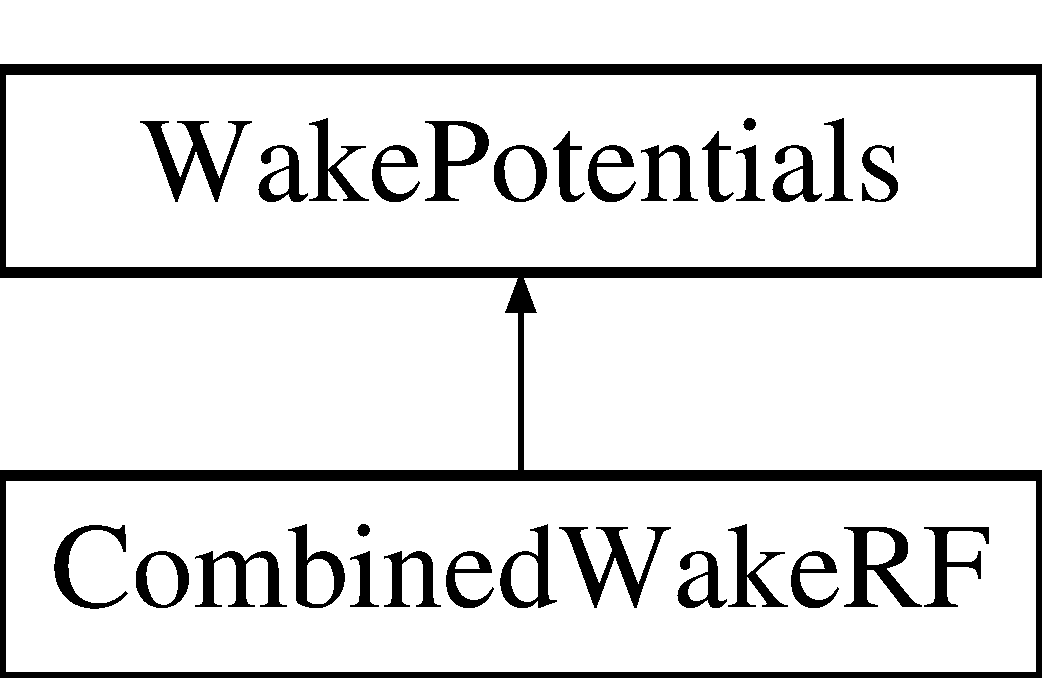
\includegraphics[height=2.000000cm]{classCombinedWakeRF}
\end{center}
\end{figure}
\subsection*{Public Member Functions}
\begin{DoxyCompactItemize}
\item 
\mbox{\Hypertarget{classCombinedWakeRF_a3251b2e49e253d5e282e8db29f93672f}\label{classCombinedWakeRF_a3251b2e49e253d5e282e8db29f93672f}} 
virtual \hyperlink{classTVec2D}{Vector2D} {\bfseries Wxy} (double x, double y) const =0
\item 
\mbox{\Hypertarget{classCombinedWakeRF_a40c2e3fc3c8df751e1f78dc9dbadf224}\label{classCombinedWakeRF_a40c2e3fc3c8df751e1f78dc9dbadf224}} 
virtual \hyperlink{classTVec2D}{Vector2D} {\bfseries Coupler\+R\+F\+Kick} (double x, double y, double phi) const =0
\end{DoxyCompactItemize}
\subsection*{Additional Inherited Members}


The documentation for this class was generated from the following file\+:\begin{DoxyCompactItemize}
\item 
/home/fallon/git/merlin-\/cmake/\+Merlin/Combined\+Wake\+R\+F.\+h\end{DoxyCompactItemize}

\hypertarget{classComplex}{}\section{Complex Class Reference}
\label{classComplex}\index{Complex@{Complex}}
\subsection*{Public Types}
\begin{DoxyCompactItemize}
\item 
\mbox{\Hypertarget{classComplex_acc42f0a27ce00262073f8eeaa34d2b33}\label{classComplex_acc42f0a27ce00262073f8eeaa34d2b33}} 
typedef double {\bfseries value\+\_\+type}
\end{DoxyCompactItemize}
\subsection*{Public Member Functions}
\begin{DoxyCompactItemize}
\item 
\mbox{\Hypertarget{classComplex_a312e4b19146128408fb06e0150b0faf6}\label{classComplex_a312e4b19146128408fb06e0150b0faf6}} 
double {\bfseries real} () const
\item 
\mbox{\Hypertarget{classComplex_af8aacf982e2e6c142921bc850f6dc974}\label{classComplex_af8aacf982e2e6c142921bc850f6dc974}} 
double {\bfseries imag} () const
\item 
\mbox{\Hypertarget{classComplex_aaa379be764626b09b66055ba1500567c}\label{classComplex_aaa379be764626b09b66055ba1500567c}} 
void {\bfseries real} (double re)
\item 
\mbox{\Hypertarget{classComplex_a72fdcc794ef364082c293e04d5373b30}\label{classComplex_a72fdcc794ef364082c293e04d5373b30}} 
void {\bfseries imag} (double im)
\item 
\mbox{\Hypertarget{classComplex_a26053ce38e21511f0147ac398d896edc}\label{classComplex_a26053ce38e21511f0147ac398d896edc}} 
{\bfseries Complex} (double re=0, double im=0)
\item 
\mbox{\Hypertarget{classComplex_a956a3fc04d0049607bb67cf9cd3817d0}\label{classComplex_a956a3fc04d0049607bb67cf9cd3817d0}} 
\hyperlink{classComplex}{Complex} \& {\bfseries operator+=} (const \hyperlink{classComplex}{Complex} \&rhs)
\item 
\mbox{\Hypertarget{classComplex_ae9f59191ac370070463e4669df631185}\label{classComplex_ae9f59191ac370070463e4669df631185}} 
\hyperlink{classComplex}{Complex} \& {\bfseries operator-\/=} (const \hyperlink{classComplex}{Complex} \&rhs)
\item 
\mbox{\Hypertarget{classComplex_aa4d2d37f0613b14e7b74c5afb49617d9}\label{classComplex_aa4d2d37f0613b14e7b74c5afb49617d9}} 
\hyperlink{classComplex}{Complex} \& {\bfseries operator$\ast$=} (const \hyperlink{classComplex}{Complex} \&rhs)
\item 
\mbox{\Hypertarget{classComplex_a6cdb101e53dbaae088c7d2e3c2099f06}\label{classComplex_a6cdb101e53dbaae088c7d2e3c2099f06}} 
\hyperlink{classComplex}{Complex} \& {\bfseries operator/=} (const \hyperlink{classComplex}{Complex} \&rhs)
\item 
\mbox{\Hypertarget{classComplex_a8011d6b4dae1439794acb899bd89e644}\label{classComplex_a8011d6b4dae1439794acb899bd89e644}} 
\hyperlink{classComplex}{Complex} \& {\bfseries operator=} (double rhs)
\item 
\mbox{\Hypertarget{classComplex_a01668fb06790072b5024f1ae30330265}\label{classComplex_a01668fb06790072b5024f1ae30330265}} 
\hyperlink{classComplex}{Complex} \& {\bfseries operator+=} (double rhs)
\item 
\mbox{\Hypertarget{classComplex_ae6f003951046107e6cf9ed966cdacb4b}\label{classComplex_ae6f003951046107e6cf9ed966cdacb4b}} 
\hyperlink{classComplex}{Complex} \& {\bfseries operator-\/=} (double rhs)
\item 
\mbox{\Hypertarget{classComplex_a263612eaf143cc6d59a8080898b5f459}\label{classComplex_a263612eaf143cc6d59a8080898b5f459}} 
\hyperlink{classComplex}{Complex} \& {\bfseries operator$\ast$=} (double rhs)
\item 
\mbox{\Hypertarget{classComplex_a112c776ce33c58fff313059a4595ca40}\label{classComplex_a112c776ce33c58fff313059a4595ca40}} 
\hyperlink{classComplex}{Complex} \& {\bfseries operator/=} (double rhs)
\end{DoxyCompactItemize}
\subsection*{Friends}
\begin{DoxyCompactItemize}
\item 
\mbox{\Hypertarget{classComplex_a1e6272806b797c78f0e60b8df9e8b245}\label{classComplex_a1e6272806b797c78f0e60b8df9e8b245}} 
\hyperlink{classComplex}{Complex} {\bfseries operator+} (const \hyperlink{classComplex}{Complex} \&lhs, const \hyperlink{classComplex}{Complex} \&rhs)
\item 
\mbox{\Hypertarget{classComplex_aa515b95c56079a8b076c67b81fa29d8f}\label{classComplex_aa515b95c56079a8b076c67b81fa29d8f}} 
\hyperlink{classComplex}{Complex} {\bfseries operator+} (const \hyperlink{classComplex}{Complex} \&lhs, double rhs)
\item 
\mbox{\Hypertarget{classComplex_a6e253695b765d426941d622528fd1ce2}\label{classComplex_a6e253695b765d426941d622528fd1ce2}} 
\hyperlink{classComplex}{Complex} {\bfseries operator+} (double lhs, const \hyperlink{classComplex}{Complex} \&rhs)
\item 
\mbox{\Hypertarget{classComplex_a505282e00ae5011159bc06603f7e7748}\label{classComplex_a505282e00ae5011159bc06603f7e7748}} 
\hyperlink{classComplex}{Complex} {\bfseries operator-\/} (const \hyperlink{classComplex}{Complex} \&lhs, const \hyperlink{classComplex}{Complex} \&rhs)
\item 
\mbox{\Hypertarget{classComplex_aa35731468ad777bdf42b1b65f6b9a31f}\label{classComplex_aa35731468ad777bdf42b1b65f6b9a31f}} 
\hyperlink{classComplex}{Complex} {\bfseries operator-\/} (const \hyperlink{classComplex}{Complex} \&lhs, double rhs)
\item 
\mbox{\Hypertarget{classComplex_a25a8a3b823f6aa69b93a0cd1b911c51b}\label{classComplex_a25a8a3b823f6aa69b93a0cd1b911c51b}} 
\hyperlink{classComplex}{Complex} {\bfseries operator-\/} (double lhs, const \hyperlink{classComplex}{Complex} \&rhs)
\item 
\mbox{\Hypertarget{classComplex_ab57557ea1ebbe8d4e0a63576f692559b}\label{classComplex_ab57557ea1ebbe8d4e0a63576f692559b}} 
\hyperlink{classComplex}{Complex} {\bfseries operator$\ast$} (const \hyperlink{classComplex}{Complex} \&lhs, double rhs)
\item 
\mbox{\Hypertarget{classComplex_a9603db869212023c65ec6bcf0d76b428}\label{classComplex_a9603db869212023c65ec6bcf0d76b428}} 
\hyperlink{classComplex}{Complex} {\bfseries operator$\ast$} (double lhs, const \hyperlink{classComplex}{Complex} \&rhs)
\item 
\mbox{\Hypertarget{classComplex_a96f4f298e72a81883672eb390e151687}\label{classComplex_a96f4f298e72a81883672eb390e151687}} 
\hyperlink{classComplex}{Complex} {\bfseries operator$\ast$} (const \hyperlink{classComplex}{Complex} \&rhs, const \hyperlink{classComplex}{Complex} \&lhs)
\item 
\mbox{\Hypertarget{classComplex_a2f83f0b45c961481f4a770015987ab65}\label{classComplex_a2f83f0b45c961481f4a770015987ab65}} 
\hyperlink{classComplex}{Complex} {\bfseries operator/} (const \hyperlink{classComplex}{Complex} \&lhs, double rhs)
\item 
\mbox{\Hypertarget{classComplex_a50e2d7b7de78e5a15e875db0a0b7cd79}\label{classComplex_a50e2d7b7de78e5a15e875db0a0b7cd79}} 
\hyperlink{classComplex}{Complex} {\bfseries operator/} (double lhs, const \hyperlink{classComplex}{Complex} \&rhs)
\item 
\mbox{\Hypertarget{classComplex_a74299d39e590ee073c044e6515026e4c}\label{classComplex_a74299d39e590ee073c044e6515026e4c}} 
bool {\bfseries operator==} (const \hyperlink{classComplex}{Complex} \&lhs, const \hyperlink{classComplex}{Complex} \&rhs)
\item 
\mbox{\Hypertarget{classComplex_a038f44233af24bcbf5386cff932129c9}\label{classComplex_a038f44233af24bcbf5386cff932129c9}} 
bool {\bfseries operator!=} (const \hyperlink{classComplex}{Complex} \&lhs, const \hyperlink{classComplex}{Complex} \&rhs)
\item 
\mbox{\Hypertarget{classComplex_a7bfb3c8e6d5305a2e1fd35b65b769177}\label{classComplex_a7bfb3c8e6d5305a2e1fd35b65b769177}} 
bool {\bfseries operator==} (const \hyperlink{classComplex}{Complex} \&lhs, double rhs)
\item 
\mbox{\Hypertarget{classComplex_addc4d2972fa9b485672f6280b9662a6c}\label{classComplex_addc4d2972fa9b485672f6280b9662a6c}} 
bool {\bfseries operator==} (double lhs, const \hyperlink{classComplex}{Complex} \&rhs)
\item 
\mbox{\Hypertarget{classComplex_aa758a7e07ce04bd59ace05a8c76a32c5}\label{classComplex_aa758a7e07ce04bd59ace05a8c76a32c5}} 
bool {\bfseries operator!=} (const \hyperlink{classComplex}{Complex} \&lhs, double rhs)
\item 
\mbox{\Hypertarget{classComplex_a8a7daff739159661e2ca8d3b5567f54b}\label{classComplex_a8a7daff739159661e2ca8d3b5567f54b}} 
bool {\bfseries operator!=} (double lhs, const \hyperlink{classComplex}{Complex} \&rhs)
\item 
\mbox{\Hypertarget{classComplex_a555b5046f4568f2283dbf0da344f6568}\label{classComplex_a555b5046f4568f2283dbf0da344f6568}} 
double {\bfseries abs} (const \hyperlink{classComplex}{Complex} \&rhs)
\item 
\mbox{\Hypertarget{classComplex_aad848c12d615222511616b3429c7048f}\label{classComplex_aad848c12d615222511616b3429c7048f}} 
double {\bfseries arg} (const \hyperlink{classComplex}{Complex} \&rhs)
\item 
\mbox{\Hypertarget{classComplex_a3e1172e031ba44fa502d8a8b133eb543}\label{classComplex_a3e1172e031ba44fa502d8a8b133eb543}} 
bool {\bfseries operator$<$} (const \hyperlink{classComplex}{Complex} \&, const \hyperlink{classComplex}{Complex} \&)
\item 
\mbox{\Hypertarget{classComplex_a81f946146f25e02aa3077ca2c80afe3c}\label{classComplex_a81f946146f25e02aa3077ca2c80afe3c}} 
std\+::ostream \& {\bfseries operator$<$$<$} (std\+::ostream \&os, const \hyperlink{classComplex}{Complex} \&z)
\item 
\mbox{\Hypertarget{classComplex_aefb0d844617443b811d1b853bd54b278}\label{classComplex_aefb0d844617443b811d1b853bd54b278}} 
\hyperlink{classComplex}{Complex} {\bfseries log} (const \hyperlink{classComplex}{Complex} \&z)
\end{DoxyCompactItemize}


The documentation for this class was generated from the following file\+:\begin{DoxyCompactItemize}
\item 
/home/fallon/git/merlin-\/cmake/\+Merlin/Complex\+Def.\+h\end{DoxyCompactItemize}

\hypertarget{classComponentDivider}{}\section{Component\+Divider Class Reference}
\label{classComponentDivider}\index{Component\+Divider@{Component\+Divider}}
Inheritance diagram for Component\+Divider\+:\begin{figure}[H]
\begin{center}
\leavevmode
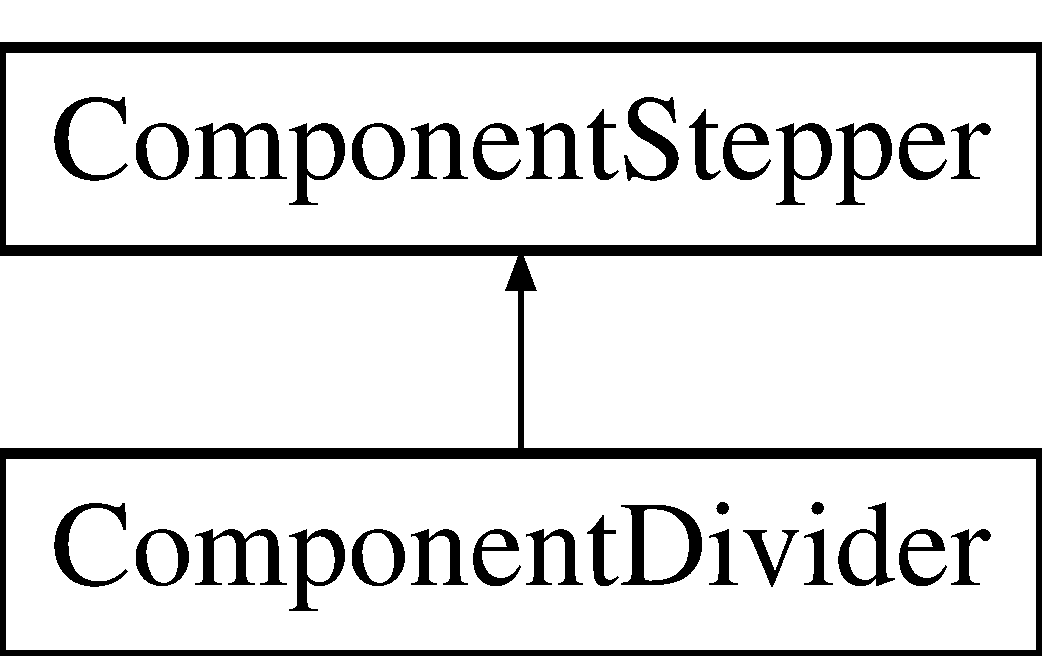
\includegraphics[height=2.000000cm]{classComponentDivider}
\end{center}
\end{figure}
\subsection*{Public Member Functions}
\begin{DoxyCompactItemize}
\item 
\mbox{\Hypertarget{classComponentDivider_aca9b92aa1de8a03d4ee464a64819de56}\label{classComponentDivider_aca9b92aa1de8a03d4ee464a64819de56}} 
{\bfseries Component\+Divider} (int ns, double min\+\_\+step=0)
\item 
\mbox{\Hypertarget{classComponentDivider_a213ba55b81fedda805634d20d79b389b}\label{classComponentDivider_a213ba55b81fedda805634d20d79b389b}} 
virtual void {\bfseries Set\+Component} (\hyperlink{classAcceleratorComponent}{Accelerator\+Component} \&cmp)
\item 
\mbox{\Hypertarget{classComponentDivider_a1cd3ca95fade3a16f66e5ed6ed617d8d}\label{classComponentDivider_a1cd3ca95fade3a16f66e5ed6ed617d8d}} 
virtual bool {\bfseries Increment} (double ds)
\item 
\mbox{\Hypertarget{classComponentDivider_a2df40bedd77f7f20312b748ab7557197}\label{classComponentDivider_a2df40bedd77f7f20312b748ab7557197}} 
virtual double {\bfseries Distance\+To\+Step\+Boundary} () const
\end{DoxyCompactItemize}


The documentation for this class was generated from the following files\+:\begin{DoxyCompactItemize}
\item 
/home/fallon/git/merlin-\/cmake/\+Merlin/Component\+Stepper.\+h\item 
/home/fallon/git/merlin-\/cmake/\+Merlin/Component\+Stepper.\+cpp\end{DoxyCompactItemize}

\hypertarget{classComponentFrame}{}\section{Component\+Frame Class Reference}
\label{classComponentFrame}\index{Component\+Frame@{Component\+Frame}}
Inheritance diagram for Component\+Frame\+:\begin{figure}[H]
\begin{center}
\leavevmode
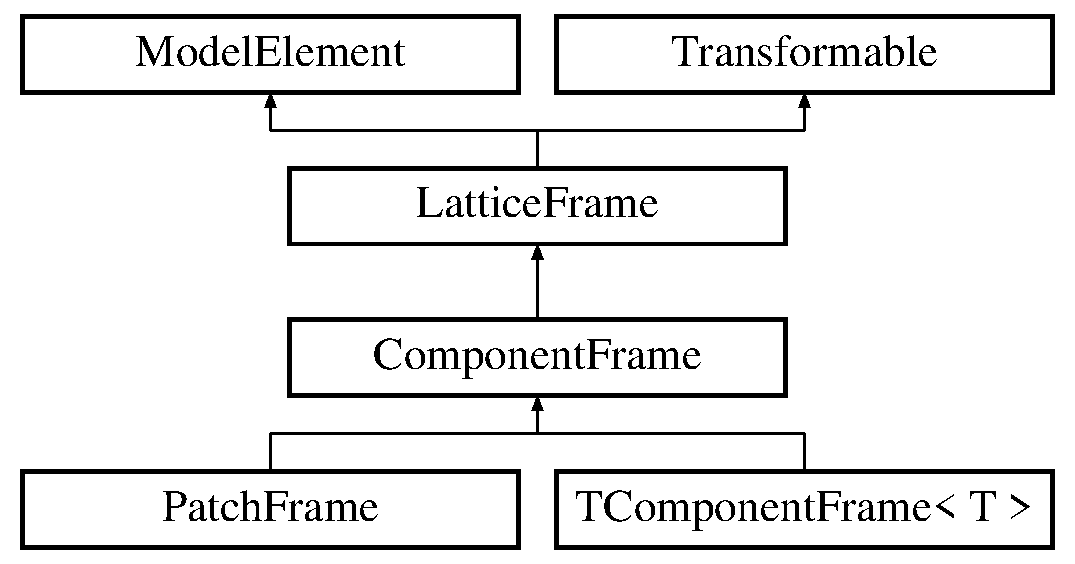
\includegraphics[height=4.000000cm]{classComponentFrame}
\end{center}
\end{figure}
\subsection*{Public Member Functions}
\begin{DoxyCompactItemize}
\item 
\mbox{\Hypertarget{classComponentFrame_a72c737f7b560d3914d87f3716331bcc8}\label{classComponentFrame_a72c737f7b560d3914d87f3716331bcc8}} 
{\bfseries Component\+Frame} (\hyperlink{classAcceleratorComponent}{Accelerator\+Component} \&ac, const string \&\hyperlink{classModelElement_aada171ead2085c75b592cf07d91bc5c2}{id}=\char`\"{}\char`\"{})
\item 
\mbox{\Hypertarget{classComponentFrame_a375129b6b8d2fdc5597612ad1d50d3f8}\label{classComponentFrame_a375129b6b8d2fdc5597612ad1d50d3f8}} 
{\bfseries Component\+Frame} (const \hyperlink{classComponentFrame}{Component\+Frame} \&rhs)
\item 
\mbox{\Hypertarget{classComponentFrame_a625e7460564cd2d4352c9d8c50b9d20c}\label{classComponentFrame_a625e7460564cd2d4352c9d8c50b9d20c}} 
\hyperlink{classAcceleratorComponent}{Accelerator\+Component} \& {\bfseries Get\+Component} ()
\item 
\mbox{\Hypertarget{classComponentFrame_a4fc89e92e4184017cd9e2847cc1aa670}\label{classComponentFrame_a4fc89e92e4184017cd9e2847cc1aa670}} 
const \hyperlink{classAcceleratorComponent}{Accelerator\+Component} \& {\bfseries Get\+Component} () const
\item 
\mbox{\Hypertarget{classComponentFrame_ac986b27ff10603bc444d24adf9083048}\label{classComponentFrame_ac986b27ff10603bc444d24adf9083048}} 
bool {\bfseries Is\+Component} () const
\item 
\mbox{\Hypertarget{classComponentFrame_aedbeb7e7ee6174ca0bb87e811507d010}\label{classComponentFrame_aedbeb7e7ee6174ca0bb87e811507d010}} 
virtual const \hyperlink{classTransform3D}{Transform3D} $\ast$ {\bfseries Get\+Entrance\+Geometry\+Patch} () const
\item 
\mbox{\Hypertarget{classComponentFrame_aebc675ac7af1342156b86e2a655212f3}\label{classComponentFrame_aebc675ac7af1342156b86e2a655212f3}} 
virtual const \hyperlink{classTransform3D}{Transform3D} $\ast$ {\bfseries Get\+Exit\+Geometry\+Patch} () const
\item 
\mbox{\Hypertarget{classComponentFrame_ab9bb6673e9023fe21fe3e82eee581fce}\label{classComponentFrame_ab9bb6673e9023fe21fe3e82eee581fce}} 
virtual void {\bfseries Invalidate} () const
\item 
virtual const string \& \hyperlink{classComponentFrame_a32bc80a48e64f286ee07519e17220248}{Get\+Name} () const
\item 
virtual const string \& \hyperlink{classComponentFrame_ab87e0e461ced7eb26a6c58bd1b04cf05}{Get\+Type} () const
\item 
virtual \hyperlink{classModelElement}{Model\+Element} $\ast$ \hyperlink{classComponentFrame_a24f6aea39b57e4b10a764877d1be6b7f}{Copy} () const
\item 
\mbox{\Hypertarget{classComponentFrame_a433281bac0ba719835fd42cc2b44c06f}\label{classComponentFrame_a433281bac0ba719835fd42cc2b44c06f}} 
void {\bfseries Set\+Beamline\+Index} (size\+\_\+t n)
\item 
\mbox{\Hypertarget{classComponentFrame_ae1ca4721d618ffb3b8a050cc4d747286}\label{classComponentFrame_ae1ca4721d618ffb3b8a050cc4d747286}} 
size\+\_\+t {\bfseries Get\+Beamline\+Index} () const
\item 
\mbox{\Hypertarget{classComponentFrame_a466620bbb459f94c54dee5e0b0c211a1}\label{classComponentFrame_a466620bbb459f94c54dee5e0b0c211a1}} 
void {\bfseries Append\+Beamline\+Indecies} (std\+::vector$<$ size\+\_\+t $>$ \&) const
\end{DoxyCompactItemize}
\subsection*{Protected Member Functions}
\begin{DoxyCompactItemize}
\item 
\mbox{\Hypertarget{classComponentFrame_a93ced219a99cf00a814bd72477add2d1}\label{classComponentFrame_a93ced219a99cf00a814bd72477add2d1}} 
{\bfseries Component\+Frame} (\hyperlink{classAcceleratorComponent}{Accelerator\+Component} $\ast$ac, const string \&\hyperlink{classModelElement_aada171ead2085c75b592cf07d91bc5c2}{id}=\char`\"{}\char`\"{})
\item 
\mbox{\Hypertarget{classComponentFrame_abe2f16cb15154490aeb3ec7c25168b0d}\label{classComponentFrame_abe2f16cb15154490aeb3ec7c25168b0d}} 
virtual bool {\bfseries Is\+Boundary\+Plane} (\hyperlink{classAcceleratorGeometry_a5c1661938176102f235836f5a8be6034}{Boundary\+Plane} p, const \hyperlink{classLatticeFrame}{Lattice\+Frame} $\ast$a\+Sub\+Frame) const
\end{DoxyCompactItemize}
\subsection*{Protected Attributes}
\begin{DoxyCompactItemize}
\item 
\mbox{\Hypertarget{classComponentFrame_acec711896d0568a381fea3f05066a4a6}\label{classComponentFrame_acec711896d0568a381fea3f05066a4a6}} 
\hyperlink{classAcceleratorComponent}{Accelerator\+Component} $\ast$ {\bfseries the\+Component}
\end{DoxyCompactItemize}
\subsection*{Additional Inherited Members}


\subsection{Member Function Documentation}
\mbox{\Hypertarget{classComponentFrame_a24f6aea39b57e4b10a764877d1be6b7f}\label{classComponentFrame_a24f6aea39b57e4b10a764877d1be6b7f}} 
\index{Component\+Frame@{Component\+Frame}!Copy@{Copy}}
\index{Copy@{Copy}!Component\+Frame@{Component\+Frame}}
\subsubsection{\texorpdfstring{Copy()}{Copy()}}
{\footnotesize\ttfamily \hyperlink{classModelElement}{Model\+Element} $\ast$ Component\+Frame\+::\+Copy (\begin{DoxyParamCaption}{ }\end{DoxyParamCaption}) const\hspace{0.3cm}{\ttfamily [virtual]}}

Virtual constructor. 

Implements \hyperlink{classModelElement_ac3ca26d649bd86a0f31a58ae09941429}{Model\+Element}.



Reimplemented in \hyperlink{classPatchFrame_a4103f544750beb79b95795c6be388c1d}{Patch\+Frame}, and \hyperlink{classTComponentFrame_a83b3faa024200e7d628451e1f8b50900}{T\+Component\+Frame$<$ T $>$}.

\mbox{\Hypertarget{classComponentFrame_a32bc80a48e64f286ee07519e17220248}\label{classComponentFrame_a32bc80a48e64f286ee07519e17220248}} 
\index{Component\+Frame@{Component\+Frame}!Get\+Name@{Get\+Name}}
\index{Get\+Name@{Get\+Name}!Component\+Frame@{Component\+Frame}}
\subsubsection{\texorpdfstring{Get\+Name()}{GetName()}}
{\footnotesize\ttfamily const string \& Component\+Frame\+::\+Get\+Name (\begin{DoxyParamCaption}{ }\end{DoxyParamCaption}) const\hspace{0.3cm}{\ttfamily [inline]}, {\ttfamily [virtual]}}

Return the name of the element. \begin{DoxyReturn}{Returns}
A string containing the name of the element. 
\end{DoxyReturn}


Reimplemented from \hyperlink{classModelElement_ae2bb7fbbbde063a49a02ea6fe22d92c4}{Model\+Element}.



Reimplemented in \hyperlink{classPatchFrame_a51ebb7649aa5fc1403bcd70925d7c85f}{Patch\+Frame}.

\mbox{\Hypertarget{classComponentFrame_ab87e0e461ced7eb26a6c58bd1b04cf05}\label{classComponentFrame_ab87e0e461ced7eb26a6c58bd1b04cf05}} 
\index{Component\+Frame@{Component\+Frame}!Get\+Type@{Get\+Type}}
\index{Get\+Type@{Get\+Type}!Component\+Frame@{Component\+Frame}}
\subsubsection{\texorpdfstring{Get\+Type()}{GetType()}}
{\footnotesize\ttfamily const string \& Component\+Frame\+::\+Get\+Type (\begin{DoxyParamCaption}{ }\end{DoxyParamCaption}) const\hspace{0.3cm}{\ttfamily [virtual]}}

Return the type string for the element. \begin{DoxyReturn}{Returns}
A string containing the type of the element. 
\end{DoxyReturn}


Implements \hyperlink{classModelElement_a04dc2e51e1999fca612eb1838ec6b271}{Model\+Element}.



Reimplemented in \hyperlink{classPatchFrame_a1ef493fda343de4400b198097db32f20}{Patch\+Frame}.



The documentation for this class was generated from the following files\+:\begin{DoxyCompactItemize}
\item 
/home/fallon/git/merlin-\/cmake/\+Merlin/Component\+Frame.\+h\item 
/home/fallon/git/merlin-\/cmake/\+Merlin/Component\+Frame.\+cpp\end{DoxyCompactItemize}

\hypertarget{classComponentIntegrator}{}\section{Component\+Integrator Class Reference}
\label{classComponentIntegrator}\index{Component\+Integrator@{Component\+Integrator}}
Inheritance diagram for Component\+Integrator\+:\begin{figure}[H]
\begin{center}
\leavevmode
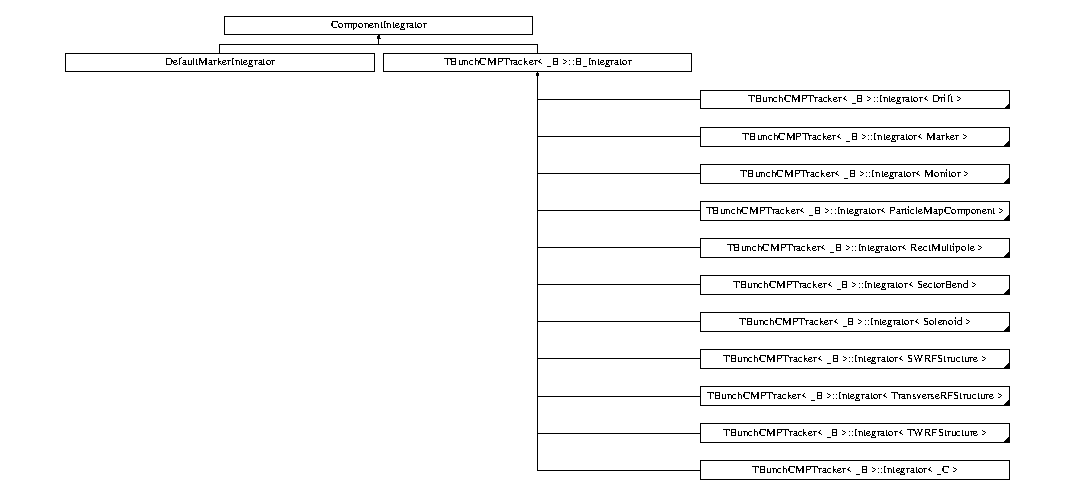
\includegraphics[height=6.222222cm]{classComponentIntegrator}
\end{center}
\end{figure}
\subsection*{Public Member Functions}
\begin{DoxyCompactItemize}
\item 
\mbox{\Hypertarget{classComponentIntegrator_a81037449593735e62c70fa6cd0c20768}\label{classComponentIntegrator_a81037449593735e62c70fa6cd0c20768}} 
void {\bfseries Track\+All} ()
\item 
\mbox{\Hypertarget{classComponentIntegrator_a5ea98e93a176d8581ac48f268173ebd5}\label{classComponentIntegrator_a5ea98e93a176d8581ac48f268173ebd5}} 
virtual double {\bfseries Track} (double ds)
\item 
\mbox{\Hypertarget{classComponentIntegrator_a9cb39d2e0d4f22344817accd711c193c}\label{classComponentIntegrator_a9cb39d2e0d4f22344817accd711c193c}} 
virtual int {\bfseries Get\+Component\+Index} () const =0
\item 
\mbox{\Hypertarget{classComponentIntegrator_ab4350e450e7f45283a9d5919859c26cc}\label{classComponentIntegrator_ab4350e450e7f45283a9d5919859c26cc}} 
double {\bfseries Get\+Integrated\+Length} () const
\item 
\mbox{\Hypertarget{classComponentIntegrator_a421b563148487d2a54200d278764fc40}\label{classComponentIntegrator_a421b563148487d2a54200d278764fc40}} 
double {\bfseries Get\+Remaining\+Length} () const
\item 
\mbox{\Hypertarget{classComponentIntegrator_afab3c609d39a252ec6c63065a509f565}\label{classComponentIntegrator_afab3c609d39a252ec6c63065a509f565}} 
bool {\bfseries Is\+Valid\+Step} (double ds) const
\item 
\mbox{\Hypertarget{classComponentIntegrator_a9953712a9b723fec4de0ce73c6c469eb}\label{classComponentIntegrator_a9953712a9b723fec4de0ce73c6c469eb}} 
virtual \hyperlink{classNumericalRange}{Float\+Range} {\bfseries Get\+Valid\+Step\+Range} () const
\item 
\mbox{\Hypertarget{classComponentIntegrator_aa44c60a7824f638dd29b22740279d2ae}\label{classComponentIntegrator_aa44c60a7824f638dd29b22740279d2ae}} 
bool {\bfseries At\+Entrance} () const
\item 
\mbox{\Hypertarget{classComponentIntegrator_a7b7ede6cc52f7bd3c763a5cb5b429900}\label{classComponentIntegrator_a7b7ede6cc52f7bd3c763a5cb5b429900}} 
bool {\bfseries At\+Exit} (double step=0) const
\end{DoxyCompactItemize}
\subsection*{Protected Member Functions}
\begin{DoxyCompactItemize}
\item 
\mbox{\Hypertarget{classComponentIntegrator_a297f809c321275632fee9d8ff5888a1c}\label{classComponentIntegrator_a297f809c321275632fee9d8ff5888a1c}} 
virtual void {\bfseries Set\+Current\+Component} (\hyperlink{classAcceleratorComponent}{Accelerator\+Component} \&a\+Component)
\item 
\mbox{\Hypertarget{classComponentIntegrator_aa9f0b7d4e71dee27739cd88fbf964e15}\label{classComponentIntegrator_aa9f0b7d4e71dee27739cd88fbf964e15}} 
virtual void {\bfseries Track\+Step} (double ds)=0
\item 
\mbox{\Hypertarget{classComponentIntegrator_aedbb23def430ead6302118934b54cafd}\label{classComponentIntegrator_aedbb23def430ead6302118934b54cafd}} 
virtual void {\bfseries Track\+Entrance} ()
\item 
\mbox{\Hypertarget{classComponentIntegrator_aca649a742f2355d7cbe0aa2297253d75}\label{classComponentIntegrator_aca649a742f2355d7cbe0aa2297253d75}} 
virtual void {\bfseries Track\+Exit} ()
\end{DoxyCompactItemize}
\subsection*{Friends}
\begin{DoxyCompactItemize}
\item 
\mbox{\Hypertarget{classComponentIntegrator_a47ec22f8d261031cdb117f49bfa14c59}\label{classComponentIntegrator_a47ec22f8d261031cdb117f49bfa14c59}} 
class {\bfseries Component\+Tracker}
\end{DoxyCompactItemize}


The documentation for this class was generated from the following file\+:\begin{DoxyCompactItemize}
\item 
/home/fallon/git/merlin-\/cmake/\+Merlin/Component\+Integrator.\+h\end{DoxyCompactItemize}

\hypertarget{classComponentStepper}{}\section{Component\+Stepper Class Reference}
\label{classComponentStepper}\index{Component\+Stepper@{Component\+Stepper}}
Inheritance diagram for Component\+Stepper\+:\begin{figure}[H]
\begin{center}
\leavevmode
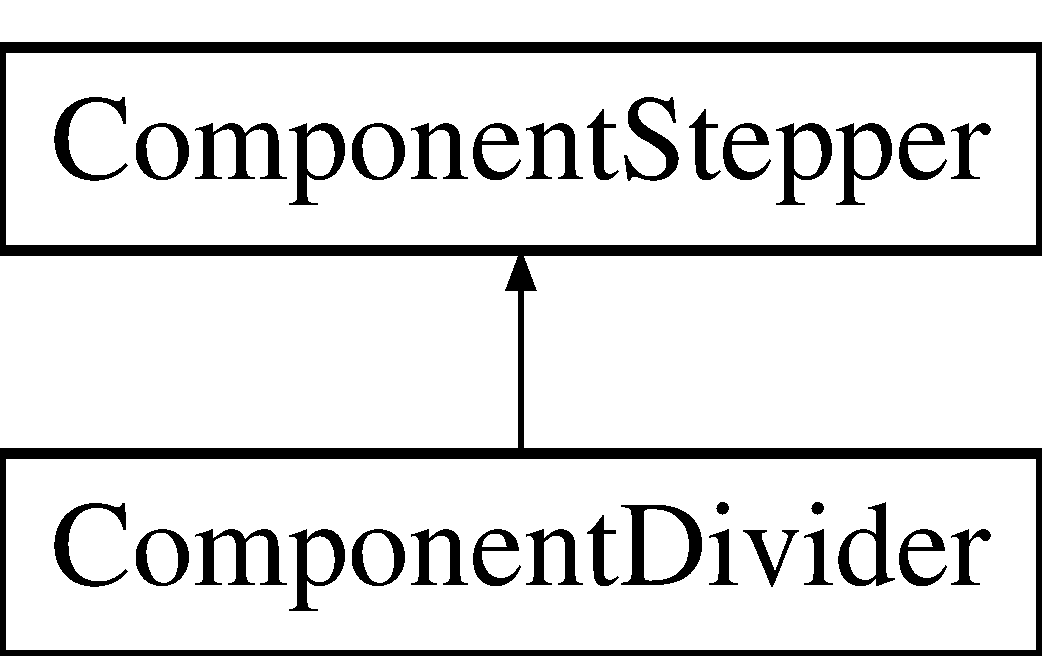
\includegraphics[height=2.000000cm]{classComponentStepper}
\end{center}
\end{figure}
\subsection*{Public Member Functions}
\begin{DoxyCompactItemize}
\item 
\mbox{\Hypertarget{classComponentStepper_a998dc625427f105d0785c84991d181e4}\label{classComponentStepper_a998dc625427f105d0785c84991d181e4}} 
virtual void {\bfseries Set\+Component} (\hyperlink{classAcceleratorComponent}{Accelerator\+Component} \&cmp)=0
\item 
\mbox{\Hypertarget{classComponentStepper_aebd8148108e7c10ac9e01a3dedfae6d2}\label{classComponentStepper_aebd8148108e7c10ac9e01a3dedfae6d2}} 
virtual bool {\bfseries Increment} (double ds)=0
\item 
\mbox{\Hypertarget{classComponentStepper_adfa9b6cc805623310bb9b7125b116842}\label{classComponentStepper_adfa9b6cc805623310bb9b7125b116842}} 
virtual double {\bfseries Distance\+To\+Step\+Boundary} () const =0
\end{DoxyCompactItemize}


The documentation for this class was generated from the following file\+:\begin{DoxyCompactItemize}
\item 
/home/fallon/git/merlin-\/cmake/\+Merlin/Component\+Stepper.\+h\end{DoxyCompactItemize}

\hypertarget{classComponentTracker}{}\section{Component\+Tracker Class Reference}
\label{classComponentTracker}\index{Component\+Tracker@{Component\+Tracker}}
Inheritance diagram for Component\+Tracker\+:\begin{figure}[H]
\begin{center}
\leavevmode
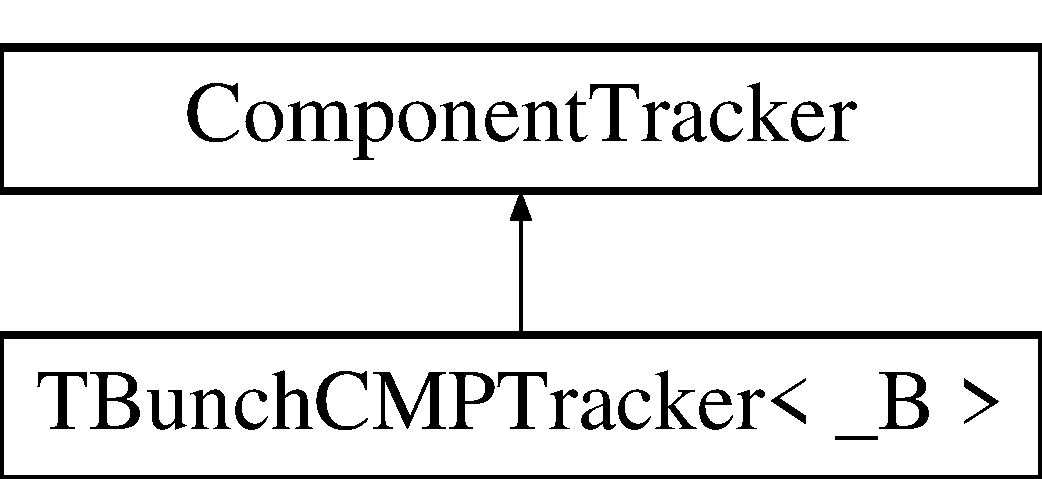
\includegraphics[height=2.000000cm]{classComponentTracker}
\end{center}
\end{figure}
\subsection*{Classes}
\begin{DoxyCompactItemize}
\item 
class \hyperlink{classComponentTracker_1_1IntegratorSet}{Integrator\+Set}
\item 
struct \hyperlink{structComponentTracker_1_1UnknownComponent}{Unknown\+Component}
\end{DoxyCompactItemize}
\subsection*{Public Types}
\begin{DoxyCompactItemize}
\item 
\mbox{\Hypertarget{classComponentTracker_a7195e1d7493af8da99857479953b088d}\label{classComponentTracker_a7195e1d7493af8da99857479953b088d}} 
enum {\bfseries State} \{ {\bfseries undefined}, 
{\bfseries initialised}, 
{\bfseries tracking}, 
{\bfseries finished}
 \}
\end{DoxyCompactItemize}
\subsection*{Public Member Functions}
\begin{DoxyCompactItemize}
\item 
\mbox{\Hypertarget{classComponentTracker_a71f34b270f618c4ca7d57bbe2a188c14}\label{classComponentTracker_a71f34b270f618c4ca7d57bbe2a188c14}} 
void {\bfseries Track} ()
\item 
\mbox{\Hypertarget{classComponentTracker_a5aa444b7ec70f30c5ed5000eb334efce}\label{classComponentTracker_a5aa444b7ec70f30c5ed5000eb334efce}} 
double {\bfseries Track\+Step} (double ds)
\item 
\mbox{\Hypertarget{classComponentTracker_ac4b090709df62a3cf8852229108df99a}\label{classComponentTracker_ac4b090709df62a3cf8852229108df99a}} 
Component\+Tracker\+::\+State {\bfseries Get\+State} () const
\item 
\mbox{\Hypertarget{classComponentTracker_adaf3f184f56c9c48f1dbbf93f3d1098c}\label{classComponentTracker_adaf3f184f56c9c48f1dbbf93f3d1098c}} 
void {\bfseries Reset} ()
\item 
\mbox{\Hypertarget{classComponentTracker_aec1cf2003378b9cb77dd06dcee8a51ad}\label{classComponentTracker_aec1cf2003378b9cb77dd06dcee8a51ad}} 
double {\bfseries Get\+Remaining\+Length} () const
\item 
\mbox{\Hypertarget{classComponentTracker_ac18f1348aea3d837ce8dd7ffb38e068f}\label{classComponentTracker_ac18f1348aea3d837ce8dd7ffb38e068f}} 
double {\bfseries Get\+Integrated\+Length} () const
\item 
\mbox{\Hypertarget{classComponentTracker_a2c56d801b3a3527d9df82b27bf3a199e}\label{classComponentTracker_a2c56d801b3a3527d9df82b27bf3a199e}} 
bool {\bfseries Select\+Integrator} (int index, \hyperlink{classAcceleratorComponent}{Accelerator\+Component} \&component)
\item 
\mbox{\Hypertarget{classComponentTracker_aa6e30205dd34c75a1631583684aa2968}\label{classComponentTracker_aa6e30205dd34c75a1631583684aa2968}} 
void {\bfseries operator()} (\hyperlink{classAcceleratorComponent}{Accelerator\+Component} $\ast$component)
\item 
\mbox{\Hypertarget{classComponentTracker_a66a893a1dc4bd8c76b6e86c34f630e72}\label{classComponentTracker_a66a893a1dc4bd8c76b6e86c34f630e72}} 
void {\bfseries Clear\+Integrator\+Set} ()
\end{DoxyCompactItemize}
\subsection*{Protected Member Functions}
\begin{DoxyCompactItemize}
\item 
\mbox{\Hypertarget{classComponentTracker_adb4cf1da1962de439a3ce3aa004fce02}\label{classComponentTracker_adb4cf1da1962de439a3ce3aa004fce02}} 
{\bfseries Component\+Tracker} (\hyperlink{classComponentTracker_1_1IntegratorSet}{Integrator\+Set} $\ast$iset)
\item 
\mbox{\Hypertarget{classComponentTracker_a121e9c22544f5dfec001e5cb0e2c5a61}\label{classComponentTracker_a121e9c22544f5dfec001e5cb0e2c5a61}} 
virtual void {\bfseries Initialise\+Integrator} (\hyperlink{classComponentIntegrator}{Component\+Integrator} $\ast$)
\item 
\mbox{\Hypertarget{classComponentTracker_a3d08499122659d456fc3bf1189e46979}\label{classComponentTracker_a3d08499122659d456fc3bf1189e46979}} 
bool {\bfseries Register} (\hyperlink{classComponentIntegrator}{Component\+Integrator} $\ast$intg)
\end{DoxyCompactItemize}


The documentation for this class was generated from the following files\+:\begin{DoxyCompactItemize}
\item 
/home/fallon/git/merlin-\/cmake/\+Merlin/Component\+Tracker.\+h\item 
/home/fallon/git/merlin-\/cmake/\+Merlin/Component\+Tracker.\+cpp\end{DoxyCompactItemize}

\hypertarget{classCompositeMaterial}{}\section{Composite\+Material Class Reference}
\label{classCompositeMaterial}\index{Composite\+Material@{Composite\+Material}}
Inheritance diagram for Composite\+Material\+:\begin{figure}[H]
\begin{center}
\leavevmode
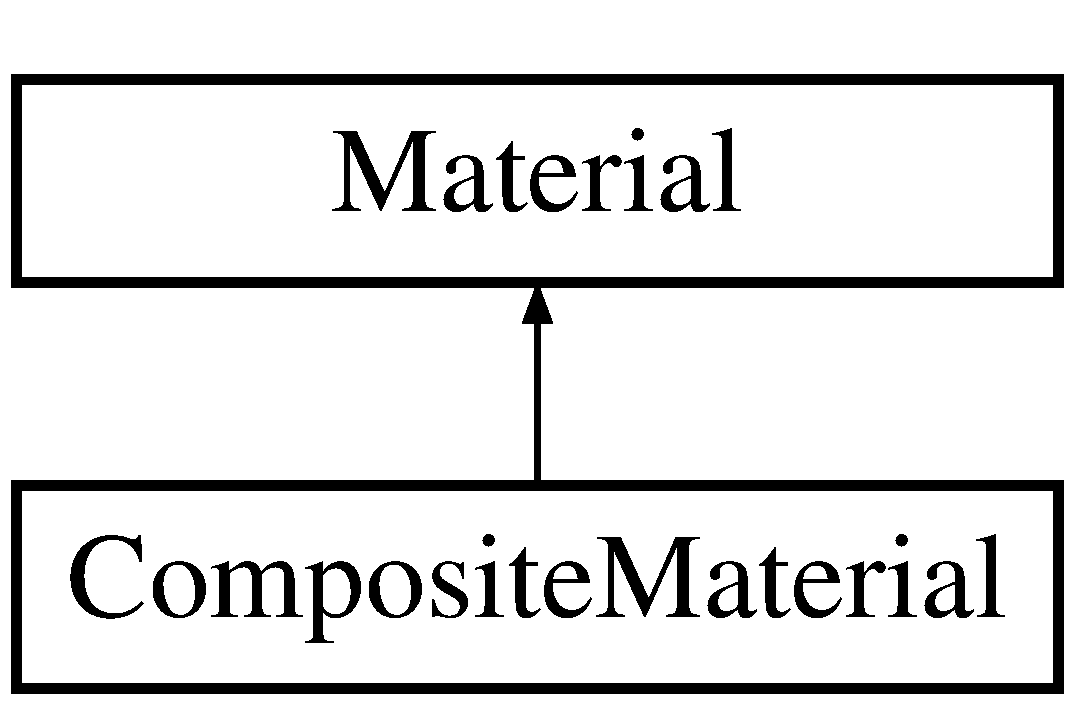
\includegraphics[height=2.000000cm]{classCompositeMaterial}
\end{center}
\end{figure}
\subsection*{Public Member Functions}
\begin{DoxyCompactItemize}
\item 
\mbox{\Hypertarget{classCompositeMaterial_a5b8d5a91e5b4926ca42e54b4d9895fc3}\label{classCompositeMaterial_a5b8d5a91e5b4926ca42e54b4d9895fc3}} 
double {\bfseries Calculate\+Electron\+Density} ()
\item 
\mbox{\Hypertarget{classCompositeMaterial_a17007f969cd002e14fb87d3a892fda72}\label{classCompositeMaterial_a17007f969cd002e14fb87d3a892fda72}} 
double {\bfseries Calculate\+Plasma\+Energy} ()
\item 
\mbox{\Hypertarget{classCompositeMaterial_a4367abb1f10eb5697ccdd7a022f4101d}\label{classCompositeMaterial_a4367abb1f10eb5697ccdd7a022f4101d}} 
double {\bfseries Calculate\+Mean\+Excitation\+Energy} ()
\item 
\mbox{\Hypertarget{classCompositeMaterial_a14b99f32cf76e8b5866d050985d95bef}\label{classCompositeMaterial_a14b99f32cf76e8b5866d050985d95bef}} 
double {\bfseries Calculate\+Radiation\+Length} ()
\item 
\mbox{\Hypertarget{classCompositeMaterial_a734c1d5d8a442a6f681130ae982d206a}\label{classCompositeMaterial_a734c1d5d8a442a6f681130ae982d206a}} 
double {\bfseries Calculate\+Sixtrackd\+Edx} ()
\item 
\mbox{\Hypertarget{classCompositeMaterial_a57fb4ce9a7fffe98982f92e78e9de545}\label{classCompositeMaterial_a57fb4ce9a7fffe98982f92e78e9de545}} 
void {\bfseries Calculate\+All\+Weighted\+Variables} ()
\item 
\mbox{\Hypertarget{classCompositeMaterial_ac07365b00ab5ab5b6e35ad2ae93a7175}\label{classCompositeMaterial_ac07365b00ab5ab5b6e35ad2ae93a7175}} 
double {\bfseries Calculate\+WeightedA} ()
\item 
\mbox{\Hypertarget{classCompositeMaterial_abad95425de71a2faf22aa4ff37abadbb}\label{classCompositeMaterial_abad95425de71a2faf22aa4ff37abadbb}} 
double {\bfseries Calculate\+WeightedZ} ()
\item 
\mbox{\Hypertarget{classCompositeMaterial_a9e0af4666694ec0fb7d79e6561dc24da}\label{classCompositeMaterial_a9e0af4666694ec0fb7d79e6561dc24da}} 
double {\bfseries Calculate\+Six\+Track\+Elastic\+Nucleus\+Cross\+Section} ()
\item 
\mbox{\Hypertarget{classCompositeMaterial_a936bfee04c5da651bc94e13c0e3e9f4a}\label{classCompositeMaterial_a936bfee04c5da651bc94e13c0e3e9f4a}} 
void {\bfseries Set\+Name} (std\+::string)
\item 
\mbox{\Hypertarget{classCompositeMaterial_aaa63c9b0d2aef14512e695d2460add6c}\label{classCompositeMaterial_aaa63c9b0d2aef14512e695d2460add6c}} 
void {\bfseries Set\+Symbol} (std\+::string)
\item 
\mbox{\Hypertarget{classCompositeMaterial_a0dbd53004231422ac9cc2d6bafb93370}\label{classCompositeMaterial_a0dbd53004231422ac9cc2d6bafb93370}} 
void {\bfseries Set\+Conductivity} (double)
\item 
\mbox{\Hypertarget{classCompositeMaterial_a61b3fd305750da332b7419f4b2dc6c44}\label{classCompositeMaterial_a61b3fd305750da332b7419f4b2dc6c44}} 
void {\bfseries Set\+Radiation\+Length} (double)
\item 
\mbox{\Hypertarget{classCompositeMaterial_aefa4007dfb9dd5bc83bbfa1cf4ab16ce}\label{classCompositeMaterial_aefa4007dfb9dd5bc83bbfa1cf4ab16ce}} 
void {\bfseries Set\+Density} (double)
\item 
\mbox{\Hypertarget{classCompositeMaterial_a044aef4bffa4067fe9f0053aee51f91b}\label{classCompositeMaterial_a044aef4bffa4067fe9f0053aee51f91b}} 
void {\bfseries Set\+Electron\+Density} (double)
\item 
\mbox{\Hypertarget{classCompositeMaterial_acc7aa25ad845eeee1d11328ed4a29b2a}\label{classCompositeMaterial_acc7aa25ad845eeee1d11328ed4a29b2a}} 
void {\bfseries Set\+Mean\+Excitation\+Energy} (double)
\item 
\mbox{\Hypertarget{classCompositeMaterial_a5185762d0b0925ef56b33b51815027b1}\label{classCompositeMaterial_a5185762d0b0925ef56b33b51815027b1}} 
void {\bfseries Set\+Plasma\+Energy} (double)
\item 
\mbox{\Hypertarget{classCompositeMaterial_aa8fb62d02d6994a16423c83b4a5180b6}\label{classCompositeMaterial_aa8fb62d02d6994a16423c83b4a5180b6}} 
void {\bfseries Set\+Sixtrackd\+Edx} (double)
\item 
\mbox{\Hypertarget{classCompositeMaterial_a614ea5d77a2df4cd63553b15852becfa}\label{classCompositeMaterial_a614ea5d77a2df4cd63553b15852becfa}} 
double {\bfseries Get\+Atomic\+Number} () const
\item 
\mbox{\Hypertarget{classCompositeMaterial_ae0ad2dbd3a5f0a6f30d61046ffff0871}\label{classCompositeMaterial_ae0ad2dbd3a5f0a6f30d61046ffff0871}} 
string {\bfseries Get\+Name} () const
\item 
\mbox{\Hypertarget{classCompositeMaterial_a96b066d69fba2729228e27af9f19449a}\label{classCompositeMaterial_a96b066d69fba2729228e27af9f19449a}} 
string {\bfseries Get\+Symbol} () const
\item 
\mbox{\Hypertarget{classCompositeMaterial_a569c8070e0a7df2d13e19ebf6b3c1310}\label{classCompositeMaterial_a569c8070e0a7df2d13e19ebf6b3c1310}} 
double {\bfseries Get\+Atomic\+Mass} () const
\item 
\mbox{\Hypertarget{classCompositeMaterial_a94f891493c118a7168906a665cdc4820}\label{classCompositeMaterial_a94f891493c118a7168906a665cdc4820}} 
double {\bfseries Get\+Conductivity} () const
\item 
\mbox{\Hypertarget{classCompositeMaterial_a75038d643406370fb57e2b4d718fbc24}\label{classCompositeMaterial_a75038d643406370fb57e2b4d718fbc24}} 
double {\bfseries Get\+Radiation\+Length} () const
\item 
\mbox{\Hypertarget{classCompositeMaterial_af6662ed3ee081a64f87d0c2de80cd621}\label{classCompositeMaterial_af6662ed3ee081a64f87d0c2de80cd621}} 
double {\bfseries Get\+Radiation\+Length\+InM} () const
\item 
\mbox{\Hypertarget{classCompositeMaterial_a666adf4b2976890c87dc9f750a9d82ed}\label{classCompositeMaterial_a666adf4b2976890c87dc9f750a9d82ed}} 
double {\bfseries Get\+Density} () const
\item 
\mbox{\Hypertarget{classCompositeMaterial_a7c29bdfc7d50f9b35edcfcd78466ac5c}\label{classCompositeMaterial_a7c29bdfc7d50f9b35edcfcd78466ac5c}} 
double {\bfseries Get\+Electron\+Density} () const
\item 
\mbox{\Hypertarget{classCompositeMaterial_ae6b0125c73e34217daf343a382d436b9}\label{classCompositeMaterial_ae6b0125c73e34217daf343a382d436b9}} 
double {\bfseries Get\+Mean\+Excitation\+Energy} () const
\item 
\mbox{\Hypertarget{classCompositeMaterial_a657c72b582b8cd47f2d543f62efdc077}\label{classCompositeMaterial_a657c72b582b8cd47f2d543f62efdc077}} 
double {\bfseries Get\+Plasma\+Energy} () const
\item 
\mbox{\Hypertarget{classCompositeMaterial_a02b8233ff4fd1317dbbca3e34dac2cac}\label{classCompositeMaterial_a02b8233ff4fd1317dbbca3e34dac2cac}} 
double {\bfseries Get\+Sixtrack\+Total\+Nucleus\+Cross\+Section} () const
\item 
\mbox{\Hypertarget{classCompositeMaterial_a290910e39c9b00605c148af0c2db53eb}\label{classCompositeMaterial_a290910e39c9b00605c148af0c2db53eb}} 
double {\bfseries Get\+Sixtrack\+Inelastic\+Nucleus\+Cross\+Section} () const
\item 
\mbox{\Hypertarget{classCompositeMaterial_ae8fdb12824bc47c073c53fe88ff6fa39}\label{classCompositeMaterial_ae8fdb12824bc47c073c53fe88ff6fa39}} 
double {\bfseries Get\+Sixtrack\+Rutherford\+Cross\+Section} () const
\item 
\mbox{\Hypertarget{classCompositeMaterial_aaebafbc87f92617435eadf08443d7553}\label{classCompositeMaterial_aaebafbc87f92617435eadf08443d7553}} 
double {\bfseries Get\+Sixtrackd\+Edx} () const
\item 
\mbox{\Hypertarget{classCompositeMaterial_ac5ed48551361a5ddd874d50861e55e48}\label{classCompositeMaterial_ac5ed48551361a5ddd874d50861e55e48}} 
double {\bfseries Get\+Sixtrack\+Nuclear\+Slope} () const
\item 
\mbox{\Hypertarget{classCompositeMaterial_a55e5872e47265b1c508e2703fc11136f}\label{classCompositeMaterial_a55e5872e47265b1c508e2703fc11136f}} 
bool {\bfseries Verify\+Material} () const
\item 
\mbox{\Hypertarget{classCompositeMaterial_a79cc20acca42097c03158e7226577c30}\label{classCompositeMaterial_a79cc20acca42097c03158e7226577c30}} 
bool {\bfseries Add\+Material\+By\+Mass\+Fraction} (\hyperlink{classMaterial}{Material} $\ast$, double)
\item 
\mbox{\Hypertarget{classCompositeMaterial_a57c206edc2c73a2538adac685e920a67}\label{classCompositeMaterial_a57c206edc2c73a2538adac685e920a67}} 
bool {\bfseries Add\+Material\+By\+Number\+Fraction} (\hyperlink{classMaterial}{Material} $\ast$, double)
\item 
\mbox{\Hypertarget{classCompositeMaterial_a1b18895aa44371dbb3ba083551bca374}\label{classCompositeMaterial_a1b18895aa44371dbb3ba083551bca374}} 
\hyperlink{classMaterial}{Material} $\ast$ {\bfseries Select\+Random\+Material} ()
\item 
\mbox{\Hypertarget{classCompositeMaterial_a9e554e29728b41919a889c14fdbceb4e}\label{classCompositeMaterial_a9e554e29728b41919a889c14fdbceb4e}} 
\hyperlink{classMaterial}{Material} $\ast$ {\bfseries Get\+Current\+Material} ()
\item 
\mbox{\Hypertarget{classCompositeMaterial_aaa3e26958a021b1d36c5e6d845a3658d}\label{classCompositeMaterial_aaa3e26958a021b1d36c5e6d845a3658d}} 
bool {\bfseries Assemble} ()
\item 
\mbox{\Hypertarget{classCompositeMaterial_a1624e66e7aeac60d853113f5fc43d634}\label{classCompositeMaterial_a1624e66e7aeac60d853113f5fc43d634}} 
bool {\bfseries Is\+Assembled} ()
\item 
\mbox{\Hypertarget{classCompositeMaterial_a50db7787a5a2b4399798dca825b8ab1d}\label{classCompositeMaterial_a50db7787a5a2b4399798dca825b8ab1d}} 
virtual bool {\bfseries Is\+Mixture} () const
\item 
\mbox{\Hypertarget{classCompositeMaterial_a179b0ed456a5f2177ca905a441a7e411}\label{classCompositeMaterial_a179b0ed456a5f2177ca905a441a7e411}} 
vector$<$ pair$<$ string, double $>$ $>$ {\bfseries Get\+Constituent\+Elements} ()
\end{DoxyCompactItemize}
\subsection*{Additional Inherited Members}


The documentation for this class was generated from the following files\+:\begin{DoxyCompactItemize}
\item 
/home/fallon/git/merlin-\/cmake/\+Merlin/Composite\+Material.\+h\item 
/home/fallon/git/merlin-\/cmake/\+Merlin/Composite\+Material.\+cpp\end{DoxyCompactItemize}

\hypertarget{classTLAS_1_1ConstSubMatrix}{}\section{T\+L\+AS\+:\+:Const\+Sub\+Matrix$<$ T $>$ Class Template Reference}
\label{classTLAS_1_1ConstSubMatrix}\index{T\+L\+A\+S\+::\+Const\+Sub\+Matrix$<$ T $>$@{T\+L\+A\+S\+::\+Const\+Sub\+Matrix$<$ T $>$}}
\subsection*{Public Types}
\begin{DoxyCompactItemize}
\item 
\mbox{\Hypertarget{classTLAS_1_1ConstSubMatrix_a8b65c964e230e32c876de94fc085469b}\label{classTLAS_1_1ConstSubMatrix_a8b65c964e230e32c876de94fc085469b}} 
typedef T {\bfseries value\+\_\+type}
\item 
\mbox{\Hypertarget{classTLAS_1_1ConstSubMatrix_ae193711f50b2937cd818fe4a4b71c4dc}\label{classTLAS_1_1ConstSubMatrix_ae193711f50b2937cd818fe4a4b71c4dc}} 
typedef \hyperlink{classTLAS_1_1Vector}{Vector}$<$ T $>$ {\bfseries vector\+\_\+type}
\item 
\mbox{\Hypertarget{classTLAS_1_1ConstSubMatrix_a4400793cf57c8dd1c96028e2bdced85e}\label{classTLAS_1_1ConstSubMatrix_a4400793cf57c8dd1c96028e2bdced85e}} 
typedef \hyperlink{classTLAS_1_1Matrix}{Matrix}$<$ T $>$ {\bfseries matrix\+\_\+type}
\end{DoxyCompactItemize}
\subsection*{Public Member Functions}
\begin{DoxyCompactItemize}
\item 
\mbox{\Hypertarget{classTLAS_1_1ConstSubMatrix_a53d63cd02b0e70a2a4590303f8d23624}\label{classTLAS_1_1ConstSubMatrix_a53d63cd02b0e70a2a4590303f8d23624}} 
T {\bfseries operator()} (Subscript i, Subscript j) const
\item 
\mbox{\Hypertarget{classTLAS_1_1ConstSubMatrix_ac92b5ac8a595494a19779540b3c241a4}\label{classTLAS_1_1ConstSubMatrix_ac92b5ac8a595494a19779540b3c241a4}} 
{\bfseries operator Matrix$<$ T $>$} () const
\item 
\mbox{\Hypertarget{classTLAS_1_1ConstSubMatrix_a48e08e979b2416fa3c560fa85a8efe52}\label{classTLAS_1_1ConstSubMatrix_a48e08e979b2416fa3c560fa85a8efe52}} 
Dimension {\bfseries nrows} () const
\item 
\mbox{\Hypertarget{classTLAS_1_1ConstSubMatrix_a57b0802f01e8e8e8f8ae2b394823508a}\label{classTLAS_1_1ConstSubMatrix_a57b0802f01e8e8e8f8ae2b394823508a}} 
Dimension {\bfseries ncols} () const
\item 
\mbox{\Hypertarget{classTLAS_1_1ConstSubMatrix_a7a9bb970ebcd2fca652a97711889acce}\label{classTLAS_1_1ConstSubMatrix_a7a9bb970ebcd2fca652a97711889acce}} 
\hyperlink{structTLAS_1_1MatrixDim}{Matrix\+Dim} {\bfseries dim} () const
\end{DoxyCompactItemize}
\subsection*{Friends}
\begin{DoxyCompactItemize}
\item 
\mbox{\Hypertarget{classTLAS_1_1ConstSubMatrix_a17fc06682c9f9c46f1e0e38b7af25b80}\label{classTLAS_1_1ConstSubMatrix_a17fc06682c9f9c46f1e0e38b7af25b80}} 
class {\bfseries Matrix$<$ T $>$}
\item 
\mbox{\Hypertarget{classTLAS_1_1ConstSubMatrix_a46c149b98c38cb0aa6399812693f1db0}\label{classTLAS_1_1ConstSubMatrix_a46c149b98c38cb0aa6399812693f1db0}} 
class {\bfseries Sub\+Matrix$<$ T $>$}
\end{DoxyCompactItemize}


The documentation for this class was generated from the following file\+:\begin{DoxyCompactItemize}
\item 
/home/fallon/git/merlin-\/cmake/\+Merlin/T\+Matrix\+Lib.\+h\end{DoxyCompactItemize}

\hypertarget{classTLAS_1_1ConstSubVector}{}\section{T\+L\+AS\+:\+:Const\+Sub\+Vector$<$ T $>$ Class Template Reference}
\label{classTLAS_1_1ConstSubVector}\index{T\+L\+A\+S\+::\+Const\+Sub\+Vector$<$ T $>$@{T\+L\+A\+S\+::\+Const\+Sub\+Vector$<$ T $>$}}
\subsection*{Public Types}
\begin{DoxyCompactItemize}
\item 
\mbox{\Hypertarget{classTLAS_1_1ConstSubVector_a2416a9fbe9300ad488a9d57dd0eb5c03}\label{classTLAS_1_1ConstSubVector_a2416a9fbe9300ad488a9d57dd0eb5c03}} 
typedef T {\bfseries value\+\_\+type}
\item 
\mbox{\Hypertarget{classTLAS_1_1ConstSubVector_a7778cbe85ee868cfc841fbb4a1c4b85e}\label{classTLAS_1_1ConstSubVector_a7778cbe85ee868cfc841fbb4a1c4b85e}} 
typedef \hyperlink{classTLAS_1_1Vector}{Vector}$<$ T $>$ {\bfseries vector\+\_\+type}
\item 
\mbox{\Hypertarget{classTLAS_1_1ConstSubVector_a84fb99ac9f91af1585c623b2c830a320}\label{classTLAS_1_1ConstSubVector_a84fb99ac9f91af1585c623b2c830a320}} 
typedef \hyperlink{classTLAS_1_1Matrix}{Matrix}$<$ T $>$ {\bfseries matrix\+\_\+type}
\end{DoxyCompactItemize}
\subsection*{Public Member Functions}
\begin{DoxyCompactItemize}
\item 
\mbox{\Hypertarget{classTLAS_1_1ConstSubVector_a1849978296470dbb98243fc98de71b1b}\label{classTLAS_1_1ConstSubVector_a1849978296470dbb98243fc98de71b1b}} 
T {\bfseries operator()} (Subscript i) const
\item 
\mbox{\Hypertarget{classTLAS_1_1ConstSubVector_a5a99e709bfa9737783c212f8793965fa}\label{classTLAS_1_1ConstSubVector_a5a99e709bfa9737783c212f8793965fa}} 
T {\bfseries operator\mbox{[}$\,$\mbox{]}} (Subscript i) const
\item 
\mbox{\Hypertarget{classTLAS_1_1ConstSubVector_a0d6d7c2c0b471ece68d3759e0774c057}\label{classTLAS_1_1ConstSubVector_a0d6d7c2c0b471ece68d3759e0774c057}} 
{\bfseries operator Vector$<$ T $>$} () const
\item 
\mbox{\Hypertarget{classTLAS_1_1ConstSubVector_a5611a4a21dbfc649de757f51c9681a6b}\label{classTLAS_1_1ConstSubVector_a5611a4a21dbfc649de757f51c9681a6b}} 
Dimension {\bfseries size} () const
\item 
\mbox{\Hypertarget{classTLAS_1_1ConstSubVector_a5304fc461f1dcb4bb8d3e74cde085047}\label{classTLAS_1_1ConstSubVector_a5304fc461f1dcb4bb8d3e74cde085047}} 
{\bfseries Const\+Sub\+Vector} (const \hyperlink{classTLAS_1_1ConstSubVector}{Const\+Sub\+Vector}$<$ T $>$ \&v)
\item 
\mbox{\Hypertarget{classTLAS_1_1ConstSubVector_a6d08e03330d9265b3900592541313a1e}\label{classTLAS_1_1ConstSubVector_a6d08e03330d9265b3900592541313a1e}} 
\hyperlink{classTLAS_1_1ConstSubVector}{Const\+Sub\+Vector}$<$ T $>$ \& {\bfseries operator=} (const \hyperlink{classTLAS_1_1ConstSubVector}{Const\+Sub\+Vector}$<$ T $>$ \&)
\end{DoxyCompactItemize}
\subsection*{Public Attributes}
\begin{DoxyCompactItemize}
\item 
\mbox{\Hypertarget{classTLAS_1_1ConstSubVector_a966402cc19fadb2306554d63d7998b37}\label{classTLAS_1_1ConstSubVector_a966402cc19fadb2306554d63d7998b37}} 
{\bfseries V\+E\+C\+\_\+\+T\+Y\+P\+E\+\_\+\+D\+E\+FS}
\end{DoxyCompactItemize}
\subsection*{Friends}
\begin{DoxyCompactItemize}
\item 
\mbox{\Hypertarget{classTLAS_1_1ConstSubVector_a17fc06682c9f9c46f1e0e38b7af25b80}\label{classTLAS_1_1ConstSubVector_a17fc06682c9f9c46f1e0e38b7af25b80}} 
class {\bfseries Matrix$<$ T $>$}
\item 
\mbox{\Hypertarget{classTLAS_1_1ConstSubVector_a07857ea092bfd5d08a811e05ad544204}\label{classTLAS_1_1ConstSubVector_a07857ea092bfd5d08a811e05ad544204}} 
class {\bfseries Vector$<$ T $>$}
\item 
\mbox{\Hypertarget{classTLAS_1_1ConstSubVector_ae8eafab737fa8fc043dfc78dbbc714e9}\label{classTLAS_1_1ConstSubVector_ae8eafab737fa8fc043dfc78dbbc714e9}} 
class {\bfseries Sub\+Vector$<$ T $>$}
\end{DoxyCompactItemize}


The documentation for this class was generated from the following file\+:\begin{DoxyCompactItemize}
\item 
/home/fallon/git/merlin-\/cmake/\+Merlin/T\+Matrix\+Lib.\+h\end{DoxyCompactItemize}

\hypertarget{classTLAS_1_1ConvergenceFailure}{}\section{T\+L\+AS\+:\+:Convergence\+Failure Class Reference}
\label{classTLAS_1_1ConvergenceFailure}\index{T\+L\+A\+S\+::\+Convergence\+Failure@{T\+L\+A\+S\+::\+Convergence\+Failure}}


The documentation for this class was generated from the following file\+:\begin{DoxyCompactItemize}
\item 
/home/fallon/git/merlin-\/cmake/\+Merlin/T\+L\+A\+S.\+h\end{DoxyCompactItemize}

\hypertarget{structCopyLatticeFunction}{}\section{Copy\+Lattice\+Function Struct Reference}
\label{structCopyLatticeFunction}\index{Copy\+Lattice\+Function@{Copy\+Lattice\+Function}}
\subsection*{Public Member Functions}
\begin{DoxyCompactItemize}
\item 
\mbox{\Hypertarget{structCopyLatticeFunction_ad5cdcc7c3870241cff21581bf92e69a0}\label{structCopyLatticeFunction_ad5cdcc7c3870241cff21581bf92e69a0}} 
{\bfseries Copy\+Lattice\+Function} (vectorlfn \&copy)
\item 
\mbox{\Hypertarget{structCopyLatticeFunction_a394aaff7aaf33ca3b41546781d46eb72}\label{structCopyLatticeFunction_a394aaff7aaf33ca3b41546781d46eb72}} 
void {\bfseries operator()} (\hyperlink{classLatticeFunction}{Lattice\+Function} $\ast$lfn)
\end{DoxyCompactItemize}


The documentation for this struct was generated from the following file\+:\begin{DoxyCompactItemize}
\item 
/home/fallon/git/merlin-\/cmake/\+Merlin/Lattice\+Functions.\+cpp\end{DoxyCompactItemize}

\hypertarget{classCorrectorWinding}{}\section{Corrector\+Winding Class Reference}
\label{classCorrectorWinding}\index{Corrector\+Winding@{Corrector\+Winding}}
Inheritance diagram for Corrector\+Winding\+:\begin{figure}[H]
\begin{center}
\leavevmode
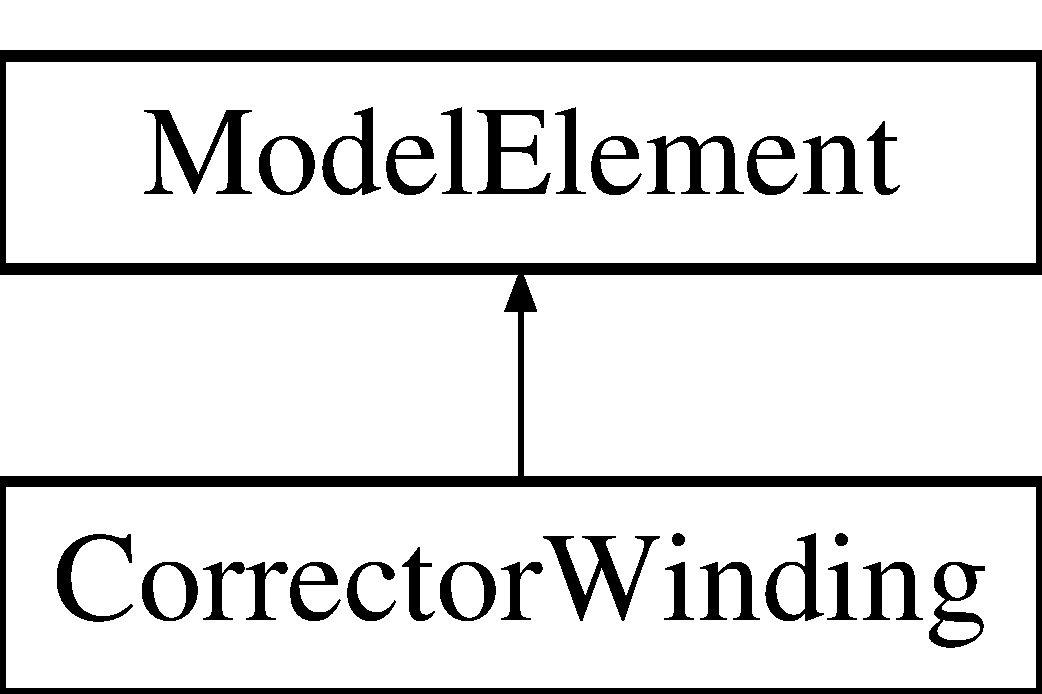
\includegraphics[height=2.000000cm]{classCorrectorWinding}
\end{center}
\end{figure}
\subsection*{Public Member Functions}
\begin{DoxyCompactItemize}
\item 
\mbox{\Hypertarget{classCorrectorWinding_a0133eff52cac0b50d79314d9b02e8b96}\label{classCorrectorWinding_a0133eff52cac0b50d79314d9b02e8b96}} 
{\bfseries Corrector\+Winding} (\hyperlink{classRectMultipole}{Rect\+Multipole} \&a\+Magnet)
\item 
\mbox{\Hypertarget{classCorrectorWinding_a8a678f90a648c17177b4d71336a56f33}\label{classCorrectorWinding_a8a678f90a648c17177b4d71336a56f33}} 
void {\bfseries Set\+Bx} (double value)
\item 
\mbox{\Hypertarget{classCorrectorWinding_adf6a894ef2ed17dfab64d91c1275145a}\label{classCorrectorWinding_adf6a894ef2ed17dfab64d91c1275145a}} 
void {\bfseries Set\+By} (double value)
\item 
\mbox{\Hypertarget{classCorrectorWinding_a822bb73822518fda0f6865974eb25731}\label{classCorrectorWinding_a822bb73822518fda0f6865974eb25731}} 
double {\bfseries Get\+Bx} () const
\item 
\mbox{\Hypertarget{classCorrectorWinding_a8b8920d4ce236592966c5c75837fef77}\label{classCorrectorWinding_a8b8920d4ce236592966c5c75837fef77}} 
double {\bfseries Get\+By} () const
\item 
virtual const string \& \hyperlink{classCorrectorWinding_afb8a04514388b2b9b0e640b606f8f47c}{Get\+Name} () const
\item 
virtual const string \& \hyperlink{classCorrectorWinding_a299195a163660e3bd13e15437a91dd91}{Get\+Type} () const
\item 
virtual \hyperlink{classModelElement}{Model\+Element} $\ast$ \hyperlink{classCorrectorWinding_adb8096ea0f8eb3743747fada685cc62c}{Copy} () const
\item 
\mbox{\Hypertarget{classCorrectorWinding_a1b7f26174afd6d35ba9e6d1e13dd4643}\label{classCorrectorWinding_a1b7f26174afd6d35ba9e6d1e13dd4643}} 
size\+\_\+t {\bfseries Get\+Beamline\+Index} () const
\item 
\mbox{\Hypertarget{classCorrectorWinding_ad3f271bc5190e0540895b4fadf4583a1}\label{classCorrectorWinding_ad3f271bc5190e0540895b4fadf4583a1}} 
void {\bfseries Append\+Beamline\+Indecies} (std\+::vector$<$ size\+\_\+t $>$ \&) const
\end{DoxyCompactItemize}
\subsection*{Additional Inherited Members}


\subsection{Member Function Documentation}
\mbox{\Hypertarget{classCorrectorWinding_adb8096ea0f8eb3743747fada685cc62c}\label{classCorrectorWinding_adb8096ea0f8eb3743747fada685cc62c}} 
\index{Corrector\+Winding@{Corrector\+Winding}!Copy@{Copy}}
\index{Copy@{Copy}!Corrector\+Winding@{Corrector\+Winding}}
\subsubsection{\texorpdfstring{Copy()}{Copy()}}
{\footnotesize\ttfamily \hyperlink{classModelElement}{Model\+Element} $\ast$ Corrector\+Winding\+::\+Copy (\begin{DoxyParamCaption}{ }\end{DoxyParamCaption}) const\hspace{0.3cm}{\ttfamily [virtual]}}

Virtual constructor. 

Implements \hyperlink{classModelElement_ac3ca26d649bd86a0f31a58ae09941429}{Model\+Element}.

\mbox{\Hypertarget{classCorrectorWinding_afb8a04514388b2b9b0e640b606f8f47c}\label{classCorrectorWinding_afb8a04514388b2b9b0e640b606f8f47c}} 
\index{Corrector\+Winding@{Corrector\+Winding}!Get\+Name@{Get\+Name}}
\index{Get\+Name@{Get\+Name}!Corrector\+Winding@{Corrector\+Winding}}
\subsubsection{\texorpdfstring{Get\+Name()}{GetName()}}
{\footnotesize\ttfamily const string \& Corrector\+Winding\+::\+Get\+Name (\begin{DoxyParamCaption}{ }\end{DoxyParamCaption}) const\hspace{0.3cm}{\ttfamily [inline]}, {\ttfamily [virtual]}}

Return the name of the element. \begin{DoxyReturn}{Returns}
A string containing the name of the element. 
\end{DoxyReturn}


Reimplemented from \hyperlink{classModelElement_ae2bb7fbbbde063a49a02ea6fe22d92c4}{Model\+Element}.

\mbox{\Hypertarget{classCorrectorWinding_a299195a163660e3bd13e15437a91dd91}\label{classCorrectorWinding_a299195a163660e3bd13e15437a91dd91}} 
\index{Corrector\+Winding@{Corrector\+Winding}!Get\+Type@{Get\+Type}}
\index{Get\+Type@{Get\+Type}!Corrector\+Winding@{Corrector\+Winding}}
\subsubsection{\texorpdfstring{Get\+Type()}{GetType()}}
{\footnotesize\ttfamily const string \& Corrector\+Winding\+::\+Get\+Type (\begin{DoxyParamCaption}{ }\end{DoxyParamCaption}) const\hspace{0.3cm}{\ttfamily [virtual]}}

Return the type string for the element. \begin{DoxyReturn}{Returns}
A string containing the type of the element. 
\end{DoxyReturn}


Implements \hyperlink{classModelElement_a04dc2e51e1999fca612eb1838ec6b271}{Model\+Element}.



The documentation for this class was generated from the following files\+:\begin{DoxyCompactItemize}
\item 
/home/fallon/git/merlin-\/cmake/\+Merlin/Corrector\+Winding.\+h\item 
/home/fallon/git/merlin-\/cmake/\+Merlin/Corrector\+Winding.\+cpp\end{DoxyCompactItemize}

\hypertarget{classParticleTracking_1_1CouplerWakeFieldProcess}{}\section{Particle\+Tracking\+:\+:Coupler\+Wake\+Field\+Process Class Reference}
\label{classParticleTracking_1_1CouplerWakeFieldProcess}\index{Particle\+Tracking\+::\+Coupler\+Wake\+Field\+Process@{Particle\+Tracking\+::\+Coupler\+Wake\+Field\+Process}}
Inheritance diagram for Particle\+Tracking\+:\+:Coupler\+Wake\+Field\+Process\+:\begin{figure}[H]
\begin{center}
\leavevmode
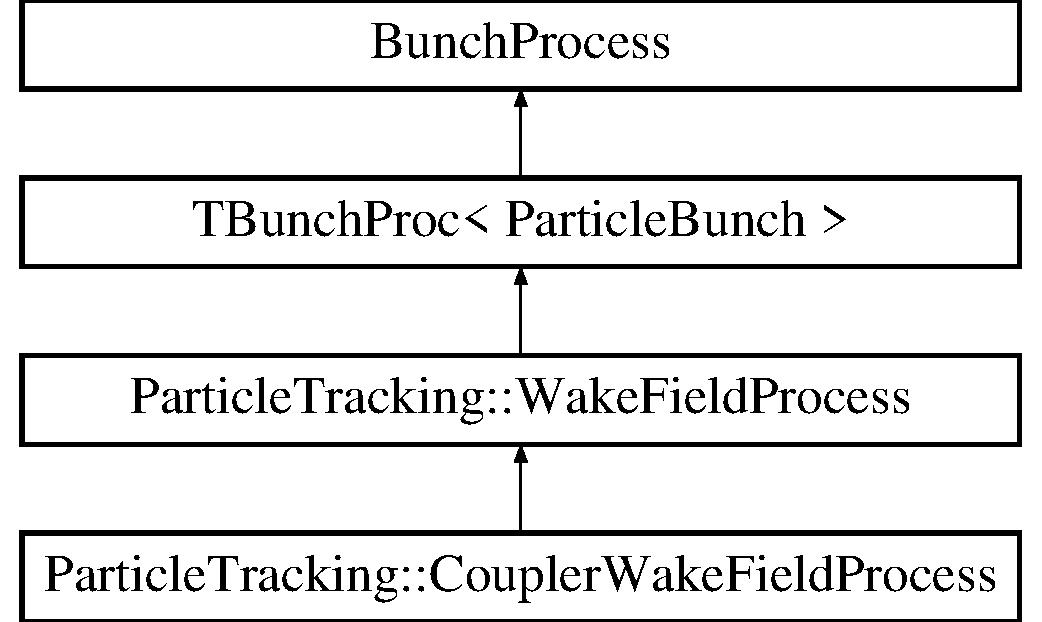
\includegraphics[height=4.000000cm]{classParticleTracking_1_1CouplerWakeFieldProcess}
\end{center}
\end{figure}
\subsection*{Public Member Functions}
\begin{DoxyCompactItemize}
\item 
\mbox{\Hypertarget{classParticleTracking_1_1CouplerWakeFieldProcess_a8f0b330d2bb20b06f3814c1bcd3e759d}\label{classParticleTracking_1_1CouplerWakeFieldProcess_a8f0b330d2bb20b06f3814c1bcd3e759d}} 
{\bfseries Coupler\+Wake\+Field\+Process} (int prio, size\+\_\+t nb=100, double ns=3.\+0)
\item 
\mbox{\Hypertarget{classParticleTracking_1_1CouplerWakeFieldProcess_a3c438187fd0e8b61073ca5dbac2c938d}\label{classParticleTracking_1_1CouplerWakeFieldProcess_a3c438187fd0e8b61073ca5dbac2c938d}} 
virtual void {\bfseries Set\+Current\+Component} (\hyperlink{classAcceleratorComponent}{Accelerator\+Component} \&component)
\item 
\mbox{\Hypertarget{classParticleTracking_1_1CouplerWakeFieldProcess_a035ec04f75196141d68da7430196b5f0}\label{classParticleTracking_1_1CouplerWakeFieldProcess_a035ec04f75196141d68da7430196b5f0}} 
virtual void {\bfseries Calculate\+WakeT} ()
\end{DoxyCompactItemize}
\subsection*{Additional Inherited Members}


The documentation for this class was generated from the following files\+:\begin{DoxyCompactItemize}
\item 
/home/fallon/git/merlin-\/cmake/\+Merlin/Coupler\+Wake\+Field\+Process.\+h\item 
/home/fallon/git/merlin-\/cmake/\+Merlin/Coupler\+Wake\+Field\+Process.\+cpp\end{DoxyCompactItemize}

\hypertarget{classCrabMarker}{}\section{Crab\+Marker Class Reference}
\label{classCrabMarker}\index{Crab\+Marker@{Crab\+Marker}}
Inheritance diagram for Crab\+Marker\+:\begin{figure}[H]
\begin{center}
\leavevmode
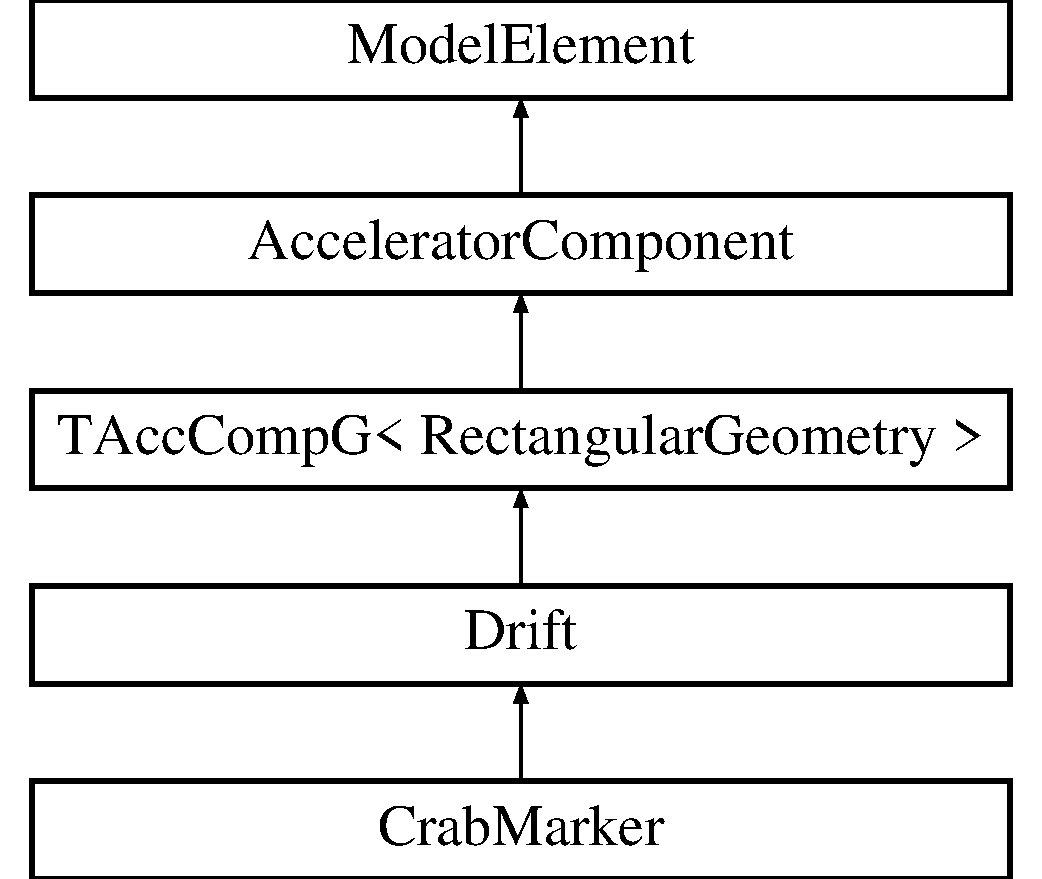
\includegraphics[height=5.000000cm]{classCrabMarker}
\end{center}
\end{figure}
\subsection*{Public Member Functions}
\begin{DoxyCompactItemize}
\item 
\mbox{\Hypertarget{classCrabMarker_ae029d5f0fce67401d5274cf7b19c193c}\label{classCrabMarker_ae029d5f0fce67401d5274cf7b19c193c}} 
{\bfseries Crab\+Marker} (const string \&\hyperlink{classModelElement_aada171ead2085c75b592cf07d91bc5c2}{id}, double len)
\item 
\mbox{\Hypertarget{classCrabMarker_a5fcb632e0f9788dec2494a3d8e67fa71}\label{classCrabMarker_a5fcb632e0f9788dec2494a3d8e67fa71}} 
{\bfseries Crab\+Marker} (const string \&\hyperlink{classModelElement_aada171ead2085c75b592cf07d91bc5c2}{id}, double len, double mux, double muy)
\item 
virtual const string \& \hyperlink{classCrabMarker_a45ab65449808d5072eb033858c2d961a}{Get\+Type} () const
\item 
virtual int \hyperlink{classCrabMarker_ae8678c41613db9792f84faf3feb88f2b}{Get\+Index} () const
\item 
virtual void \hyperlink{classCrabMarker_ab29822625603a198dc7623979ed1bb3b}{Prepare\+Tracker} (\hyperlink{classComponentTracker}{Component\+Tracker} \&a\+Tracker)
\item 
virtual void \hyperlink{classCrabMarker_a4b60620517f65b4e1f557300a3dbe89b}{Rotate\+Y180} ()
\item 
virtual \hyperlink{classModelElement}{Model\+Element} $\ast$ \hyperlink{classCrabMarker_acd6d5d5a310e985f191443b42d8abc72}{Copy} () const
\item 
\mbox{\Hypertarget{classCrabMarker_a11d4fee61122e5c5ce49aefac64de104}\label{classCrabMarker_a11d4fee61122e5c5ce49aefac64de104}} 
double {\bfseries Get\+MuX} () const
\item 
\mbox{\Hypertarget{classCrabMarker_aeb4bdc05a12bf74a267006b6c8296ff5}\label{classCrabMarker_aeb4bdc05a12bf74a267006b6c8296ff5}} 
double {\bfseries Get\+MuY} () const
\item 
\mbox{\Hypertarget{classCrabMarker_a69706d4550b59d629de7d407e8acb378}\label{classCrabMarker_a69706d4550b59d629de7d407e8acb378}} 
void {\bfseries Set\+MuX} (double mux)
\item 
\mbox{\Hypertarget{classCrabMarker_a0a6ced78b027536a8418a2c9496a0795}\label{classCrabMarker_a0a6ced78b027536a8418a2c9496a0795}} 
void {\bfseries Set\+MuY} (double muy)
\end{DoxyCompactItemize}
\subsection*{Static Public Attributes}
\begin{DoxyCompactItemize}
\item 
\mbox{\Hypertarget{classCrabMarker_a117b834252f16859870333f898179929}\label{classCrabMarker_a117b834252f16859870333f898179929}} 
static const int {\bfseries ID} = \hyperlink{classAcceleratorComponent_aa7ad4d39e1a488b705983842ed1ac784}{Unique\+Index}()
\end{DoxyCompactItemize}
\subsection*{Additional Inherited Members}


\subsection{Member Function Documentation}
\mbox{\Hypertarget{classCrabMarker_acd6d5d5a310e985f191443b42d8abc72}\label{classCrabMarker_acd6d5d5a310e985f191443b42d8abc72}} 
\index{Crab\+Marker@{Crab\+Marker}!Copy@{Copy}}
\index{Copy@{Copy}!Crab\+Marker@{Crab\+Marker}}
\subsubsection{\texorpdfstring{Copy()}{Copy()}}
{\footnotesize\ttfamily \hyperlink{classModelElement}{Model\+Element} $\ast$ Crab\+Marker\+::\+Copy (\begin{DoxyParamCaption}{ }\end{DoxyParamCaption}) const\hspace{0.3cm}{\ttfamily [virtual]}}

Virtual constructor. 

Reimplemented from \hyperlink{classDrift_ae47df31297596e13944364d602c95ce5}{Drift}.

\mbox{\Hypertarget{classCrabMarker_ae8678c41613db9792f84faf3feb88f2b}\label{classCrabMarker_ae8678c41613db9792f84faf3feb88f2b}} 
\index{Crab\+Marker@{Crab\+Marker}!Get\+Index@{Get\+Index}}
\index{Get\+Index@{Get\+Index}!Crab\+Marker@{Crab\+Marker}}
\subsubsection{\texorpdfstring{Get\+Index()}{GetIndex()}}
{\footnotesize\ttfamily int Crab\+Marker\+::\+Get\+Index (\begin{DoxyParamCaption}{ }\end{DoxyParamCaption}) const\hspace{0.3cm}{\ttfamily [virtual]}}

Returns the unique index for this class of accelerator components. \begin{DoxyReturn}{Returns}
An integer containing the unique index for this \hyperlink{classAcceleratorComponent}{Accelerator\+Component} type. 
\end{DoxyReturn}


Reimplemented from \hyperlink{classDrift_a19bc19d48348912f8693e3ebbf9e92f2}{Drift}.

\mbox{\Hypertarget{classCrabMarker_a45ab65449808d5072eb033858c2d961a}\label{classCrabMarker_a45ab65449808d5072eb033858c2d961a}} 
\index{Crab\+Marker@{Crab\+Marker}!Get\+Type@{Get\+Type}}
\index{Get\+Type@{Get\+Type}!Crab\+Marker@{Crab\+Marker}}
\subsubsection{\texorpdfstring{Get\+Type()}{GetType()}}
{\footnotesize\ttfamily const string \& Crab\+Marker\+::\+Get\+Type (\begin{DoxyParamCaption}{ }\end{DoxyParamCaption}) const\hspace{0.3cm}{\ttfamily [virtual]}}

Return the type string for the element. \begin{DoxyReturn}{Returns}
A string containing the type of the element. 
\end{DoxyReturn}


Reimplemented from \hyperlink{classDrift_a9f5e7d0aafd8689a4420b3d5e7b6879e}{Drift}.

\mbox{\Hypertarget{classCrabMarker_ab29822625603a198dc7623979ed1bb3b}\label{classCrabMarker_ab29822625603a198dc7623979ed1bb3b}} 
\index{Crab\+Marker@{Crab\+Marker}!Prepare\+Tracker@{Prepare\+Tracker}}
\index{Prepare\+Tracker@{Prepare\+Tracker}!Crab\+Marker@{Crab\+Marker}}
\subsubsection{\texorpdfstring{Prepare\+Tracker()}{PrepareTracker()}}
{\footnotesize\ttfamily void Crab\+Marker\+::\+Prepare\+Tracker (\begin{DoxyParamCaption}\item[{\hyperlink{classComponentTracker}{Component\+Tracker} \&}]{a\+Tracker }\end{DoxyParamCaption})\hspace{0.3cm}{\ttfamily [virtual]}}

Primary tracking interface. Prepares the specified Tracker object for tracking this component. 
\begin{DoxyParams}[1]{Parameters}
\mbox{\tt in,out}  & {\em a\+Tracker} & The tracker to prepare. \\
\hline
\end{DoxyParams}


Reimplemented from \hyperlink{classDrift_a9f3925549a0c7c99b39a1abea8546642}{Drift}.

\mbox{\Hypertarget{classCrabMarker_a4b60620517f65b4e1f557300a3dbe89b}\label{classCrabMarker_a4b60620517f65b4e1f557300a3dbe89b}} 
\index{Crab\+Marker@{Crab\+Marker}!Rotate\+Y180@{Rotate\+Y180}}
\index{Rotate\+Y180@{Rotate\+Y180}!Crab\+Marker@{Crab\+Marker}}
\subsubsection{\texorpdfstring{Rotate\+Y180()}{RotateY180()}}
{\footnotesize\ttfamily void Crab\+Marker\+::\+Rotate\+Y180 (\begin{DoxyParamCaption}{ }\end{DoxyParamCaption})\hspace{0.3cm}{\ttfamily [virtual]}}

Rotates the component 180 degrees about its local Y axis. 

Reimplemented from \hyperlink{classDrift_abf387eddfcabfc81b186080f6301ce60}{Drift}.



The documentation for this class was generated from the following files\+:\begin{DoxyCompactItemize}
\item 
/home/fallon/git/merlin-\/cmake/\+Merlin/Crab\+Marker.\+h\item 
/home/fallon/git/merlin-\/cmake/\+Merlin/Crab\+Marker.\+cpp\end{DoxyCompactItemize}

\hypertarget{classCollimation_1_1CrossSections}{}\section{Collimation\+:\+:Cross\+Sections Class Reference}
\label{classCollimation_1_1CrossSections}\index{Collimation\+::\+Cross\+Sections@{Collimation\+::\+Cross\+Sections}}
\subsection*{Public Member Functions}
\begin{DoxyCompactItemize}
\item 
\mbox{\Hypertarget{classCollimation_1_1CrossSections_af198fdf0a641898485ed0e28e1044ee3}\label{classCollimation_1_1CrossSections_af198fdf0a641898485ed0e28e1044ee3}} 
{\bfseries Cross\+Sections} (\hyperlink{classMaterial}{Material} $\ast$mat, double E, int scattertype)
\item 
\mbox{\Hypertarget{classCollimation_1_1CrossSections_ae08c93cdc037cd9e36cd53ee158b9cc3}\label{classCollimation_1_1CrossSections_ae08c93cdc037cd9e36cd53ee158b9cc3}} 
bool {\bfseries operator==} (const \hyperlink{classCollimation_1_1CrossSections}{Cross\+Sections} \&rhs)
\item 
\mbox{\Hypertarget{classCollimation_1_1CrossSections_ad5c87b9d0d93ee57e7d01b80ee4b5708}\label{classCollimation_1_1CrossSections_ad5c87b9d0d93ee57e7d01b80ee4b5708}} 
void {\bfseries Configure\+Cross\+Sections} (double E0)
\item 
\mbox{\Hypertarget{classCollimation_1_1CrossSections_a7e7758d0981c978be882530ff75205a3}\label{classCollimation_1_1CrossSections_a7e7758d0981c978be882530ff75205a3}} 
double {\bfseries Get\+Total\+Mean\+Free\+Path} ()
\item 
\mbox{\Hypertarget{classCollimation_1_1CrossSections_a004c8d8142324cd8b079b8e8d83efdf6}\label{classCollimation_1_1CrossSections_a004c8d8142324cd8b079b8e8d83efdf6}} 
void {\bfseries Set\+\_\+\+E0} (double a)
\item 
\mbox{\Hypertarget{classCollimation_1_1CrossSections_a90165895d41755e3084a4208025729bf}\label{classCollimation_1_1CrossSections_a90165895d41755e3084a4208025729bf}} 
double {\bfseries Get\+\_\+\+E0} () const
\item 
\mbox{\Hypertarget{classCollimation_1_1CrossSections_ad3a26cb9585681523d27c32f69ad76e0}\label{classCollimation_1_1CrossSections_ad3a26cb9585681523d27c32f69ad76e0}} 
void {\bfseries Set\+\_\+sig\+\_\+p\+N\+\_\+tot\+\_\+ref} (double a)
\item 
\mbox{\Hypertarget{classCollimation_1_1CrossSections_a58cdd9c33d62a3588d867e6606ee8b35}\label{classCollimation_1_1CrossSections_a58cdd9c33d62a3588d867e6606ee8b35}} 
double {\bfseries Get\+\_\+sig\+\_\+p\+N\+\_\+tot\+\_\+ref} () const
\item 
\mbox{\Hypertarget{classCollimation_1_1CrossSections_a2530102210c4a3762601c1a75010da5e}\label{classCollimation_1_1CrossSections_a2530102210c4a3762601c1a75010da5e}} 
void {\bfseries Set\+\_\+sig\+\_\+p\+N\+\_\+inel\+\_\+ref} (double a)
\item 
\mbox{\Hypertarget{classCollimation_1_1CrossSections_a93034b9138f9cd2c7e2516f1a0add512}\label{classCollimation_1_1CrossSections_a93034b9138f9cd2c7e2516f1a0add512}} 
double {\bfseries Get\+\_\+sig\+\_\+p\+N\+\_\+inel\+\_\+ref} () const
\item 
\mbox{\Hypertarget{classCollimation_1_1CrossSections_a5c7133b2033f3a1ba91424b9a1a46229}\label{classCollimation_1_1CrossSections_a5c7133b2033f3a1ba91424b9a1a46229}} 
void {\bfseries Set\+\_\+sig\+\_\+\+R\+\_\+ref} (double a)
\item 
\mbox{\Hypertarget{classCollimation_1_1CrossSections_ab0d57857f18cd6b73331487d83f8ef1a}\label{classCollimation_1_1CrossSections_ab0d57857f18cd6b73331487d83f8ef1a}} 
double {\bfseries Get\+\_\+sig\+\_\+\+R\+\_\+ref} () const
\item 
\mbox{\Hypertarget{classCollimation_1_1CrossSections_aaef706a0c9445dd5945cb3f255d3faca}\label{classCollimation_1_1CrossSections_aaef706a0c9445dd5945cb3f255d3faca}} 
void {\bfseries Set\+\_\+sig\+\_\+R} (double a)
\item 
\mbox{\Hypertarget{classCollimation_1_1CrossSections_a606580f9848fb8f823034f2d837919f3}\label{classCollimation_1_1CrossSections_a606580f9848fb8f823034f2d837919f3}} 
double {\bfseries Get\+\_\+sig\+\_\+R} () const
\item 
\mbox{\Hypertarget{classCollimation_1_1CrossSections_a0cd26fa266de2917c02ec0fdd5a769b1}\label{classCollimation_1_1CrossSections_a0cd26fa266de2917c02ec0fdd5a769b1}} 
void {\bfseries Set\+\_\+sig\+\_\+pp\+\_\+tot} (double a)
\item 
\mbox{\Hypertarget{classCollimation_1_1CrossSections_a81ca6f4f323b96e735530b813a89f410}\label{classCollimation_1_1CrossSections_a81ca6f4f323b96e735530b813a89f410}} 
double {\bfseries Get\+\_\+sig\+\_\+pp\+\_\+tot} () const
\item 
\mbox{\Hypertarget{classCollimation_1_1CrossSections_ae3a984471750c040d45b109469050dce}\label{classCollimation_1_1CrossSections_ae3a984471750c040d45b109469050dce}} 
void {\bfseries Set\+\_\+sig\+\_\+pp\+\_\+el} (double a)
\item 
\mbox{\Hypertarget{classCollimation_1_1CrossSections_a475d52055ff07d199ecccdd80a0adf57}\label{classCollimation_1_1CrossSections_a475d52055ff07d199ecccdd80a0adf57}} 
double {\bfseries Get\+\_\+sig\+\_\+pp\+\_\+el} () const
\item 
\mbox{\Hypertarget{classCollimation_1_1CrossSections_a4fd7f49bad4bfe35f6211b63dabcf346}\label{classCollimation_1_1CrossSections_a4fd7f49bad4bfe35f6211b63dabcf346}} 
void {\bfseries Set\+\_\+sig\+\_\+pn\+\_\+el} (double a)
\item 
\mbox{\Hypertarget{classCollimation_1_1CrossSections_a1590877c8d2121ffb8c4e7b2582e7851}\label{classCollimation_1_1CrossSections_a1590877c8d2121ffb8c4e7b2582e7851}} 
double {\bfseries Get\+\_\+sig\+\_\+pn\+\_\+el} () const
\item 
\mbox{\Hypertarget{classCollimation_1_1CrossSections_ab449c77ff2061a721e4e4612a075525d}\label{classCollimation_1_1CrossSections_ab449c77ff2061a721e4e4612a075525d}} 
void {\bfseries Set\+\_\+sig\+\_\+pp\+\_\+sd} (double a)
\item 
\mbox{\Hypertarget{classCollimation_1_1CrossSections_a00ad39aefab3fc49aa12fa4f3a6b1f27}\label{classCollimation_1_1CrossSections_a00ad39aefab3fc49aa12fa4f3a6b1f27}} 
double {\bfseries Get\+\_\+sig\+\_\+pp\+\_\+sd} () const
\item 
\mbox{\Hypertarget{classCollimation_1_1CrossSections_a4a3b15e43375935b6b91acf6b6329df7}\label{classCollimation_1_1CrossSections_a4a3b15e43375935b6b91acf6b6329df7}} 
void {\bfseries Set\+\_\+sig\+\_\+pn\+\_\+sd} (double a)
\item 
\mbox{\Hypertarget{classCollimation_1_1CrossSections_a6f6e1c3d6ba388e16574a8f711456441}\label{classCollimation_1_1CrossSections_a6f6e1c3d6ba388e16574a8f711456441}} 
double {\bfseries Get\+\_\+sig\+\_\+pn\+\_\+sd} () const
\item 
\mbox{\Hypertarget{classCollimation_1_1CrossSections_a9095f2f9dedf4dd3e74c00c2d4de4974}\label{classCollimation_1_1CrossSections_a9095f2f9dedf4dd3e74c00c2d4de4974}} 
void {\bfseries Set\+\_\+sig\+\_\+p\+N\+\_\+tot} (double a)
\item 
\mbox{\Hypertarget{classCollimation_1_1CrossSections_a0f5aee0939a050d1787d872f34cf0103}\label{classCollimation_1_1CrossSections_a0f5aee0939a050d1787d872f34cf0103}} 
double {\bfseries Get\+\_\+sig\+\_\+p\+N\+\_\+tot} () const
\item 
\mbox{\Hypertarget{classCollimation_1_1CrossSections_a7d138a9c781b9cc38487a942aa8c3eef}\label{classCollimation_1_1CrossSections_a7d138a9c781b9cc38487a942aa8c3eef}} 
void {\bfseries Set\+\_\+sig\+\_\+p\+N\+\_\+inel} (double a)
\item 
\mbox{\Hypertarget{classCollimation_1_1CrossSections_a5e1017aec82f2727e5143552b07c7412}\label{classCollimation_1_1CrossSections_a5e1017aec82f2727e5143552b07c7412}} 
double {\bfseries Get\+\_\+sig\+\_\+p\+N\+\_\+inel} () const
\item 
\mbox{\Hypertarget{classCollimation_1_1CrossSections_a457989f96aa78e993f73130cdf455917}\label{classCollimation_1_1CrossSections_a457989f96aa78e993f73130cdf455917}} 
void {\bfseries Set\+\_\+sig\+\_\+p\+N\+\_\+el} (double a)
\item 
\mbox{\Hypertarget{classCollimation_1_1CrossSections_a3c9e3cf531ddf2eb88cd91f096a1d5c7}\label{classCollimation_1_1CrossSections_a3c9e3cf531ddf2eb88cd91f096a1d5c7}} 
double {\bfseries Get\+\_\+sig\+\_\+p\+N\+\_\+el} () const
\item 
\mbox{\Hypertarget{classCollimation_1_1CrossSections_ab0436d16d72e280d7502232bdfc36635}\label{classCollimation_1_1CrossSections_ab0436d16d72e280d7502232bdfc36635}} 
void {\bfseries Set\+\_\+lambda\+\_\+tot} (double a)
\item 
\mbox{\Hypertarget{classCollimation_1_1CrossSections_a90a5ef78a04febc2de3d8fcaac48c651}\label{classCollimation_1_1CrossSections_a90a5ef78a04febc2de3d8fcaac48c651}} 
double {\bfseries Get\+\_\+lambda\+\_\+tot} () const
\item 
\mbox{\Hypertarget{classCollimation_1_1CrossSections_afcaecf5efc63e0771c642356b4a18f4b}\label{classCollimation_1_1CrossSections_afcaecf5efc63e0771c642356b4a18f4b}} 
void {\bfseries Set\+\_\+elastic\+\_\+diff} (double a)
\item 
\mbox{\Hypertarget{classCollimation_1_1CrossSections_a77c38b00bd2171d14349a9f9d8d8c7cb}\label{classCollimation_1_1CrossSections_a77c38b00bd2171d14349a9f9d8d8c7cb}} 
double {\bfseries Get\+\_\+elastic\+\_\+diff} () const
\item 
\mbox{\Hypertarget{classCollimation_1_1CrossSections_add37bafb39df3bfc380c1d652b914248}\label{classCollimation_1_1CrossSections_add37bafb39df3bfc380c1d652b914248}} 
void {\bfseries Set\+\_\+com\+\_\+sqd} (double a)
\item 
\mbox{\Hypertarget{classCollimation_1_1CrossSections_a37d21a97bda5c09a18dee1bfbff6586e}\label{classCollimation_1_1CrossSections_a37d21a97bda5c09a18dee1bfbff6586e}} 
double {\bfseries Get\+\_\+com\+\_\+sqd} () const
\item 
\mbox{\Hypertarget{classCollimation_1_1CrossSections_a40819a0a2ed3ce4063b42ab4ec2d3cfd}\label{classCollimation_1_1CrossSections_a40819a0a2ed3ce4063b42ab4ec2d3cfd}} 
void {\bfseries Set\+\_\+density} (double a)
\item 
\mbox{\Hypertarget{classCollimation_1_1CrossSections_a969aa7158af5b0354f9a1987570943a2}\label{classCollimation_1_1CrossSections_a969aa7158af5b0354f9a1987570943a2}} 
double {\bfseries Get\+\_\+density} () const
\item 
\mbox{\Hypertarget{classCollimation_1_1CrossSections_a1c38d17e2370ebc7267ae6fbd79c7091}\label{classCollimation_1_1CrossSections_a1c38d17e2370ebc7267ae6fbd79c7091}} 
void {\bfseries Set\+\_\+atomic\+\_\+mass} (double a)
\item 
\mbox{\Hypertarget{classCollimation_1_1CrossSections_aed072de15db2d4392c27e432aedecbe2}\label{classCollimation_1_1CrossSections_aed072de15db2d4392c27e432aedecbe2}} 
double {\bfseries Get\+\_\+atomic\+\_\+mass} () const
\item 
\mbox{\Hypertarget{classCollimation_1_1CrossSections_abb26a8ab7513e1111fb57cdb818a8b03}\label{classCollimation_1_1CrossSections_abb26a8ab7513e1111fb57cdb818a8b03}} 
void {\bfseries Set\+\_\+atomic\+\_\+no} (double a)
\item 
\mbox{\Hypertarget{classCollimation_1_1CrossSections_a32823016d314982b8ec9855140369f2e}\label{classCollimation_1_1CrossSections_a32823016d314982b8ec9855140369f2e}} 
double {\bfseries Get\+\_\+atomic\+\_\+no} () const
\item 
\mbox{\Hypertarget{classCollimation_1_1CrossSections_a1b287c237264fe218afeb6b710f351f7}\label{classCollimation_1_1CrossSections_a1b287c237264fe218afeb6b710f351f7}} 
void {\bfseries Set\+\_\+scat\+\_\+type} (int a)
\item 
\mbox{\Hypertarget{classCollimation_1_1CrossSections_abec4558086c5b943c293f09a8eae6cb0}\label{classCollimation_1_1CrossSections_abec4558086c5b943c293f09a8eae6cb0}} 
int {\bfseries Get\+\_\+scat\+\_\+type} () const
\item 
\mbox{\Hypertarget{classCollimation_1_1CrossSections_a86b9cc61058db4490c9b4d08b8988475}\label{classCollimation_1_1CrossSections_a86b9cc61058db4490c9b4d08b8988475}} 
\hyperlink{classParticleTracking_1_1ppElasticScatter}{Particle\+Tracking\+::pp\+Elastic\+Scatter} $\ast$ {\bfseries Get\+Elastic\+Scatter} () const
\item 
\mbox{\Hypertarget{classCollimation_1_1CrossSections_a9e9fa09cd12cb1df1675ead3f9b6cd1b}\label{classCollimation_1_1CrossSections_a9e9fa09cd12cb1df1675ead3f9b6cd1b}} 
\hyperlink{classParticleTracking_1_1ppDiffractiveScatter}{Particle\+Tracking\+::pp\+Diffractive\+Scatter} $\ast$ {\bfseries Get\+Diffractive\+Scatter} () const
\end{DoxyCompactItemize}


The documentation for this class was generated from the following files\+:\begin{DoxyCompactItemize}
\item 
/home/fallon/git/merlin-\/cmake/\+Merlin/Cross\+Sections.\+h\item 
/home/fallon/git/merlin-\/cmake/\+Merlin/Cross\+Sections.\+cpp\end{DoxyCompactItemize}

\hypertarget{structBPM_1_1Data}{}\section{B\+PM\+:\+:Data Struct Reference}
\label{structBPM_1_1Data}\index{B\+P\+M\+::\+Data@{B\+P\+M\+::\+Data}}
\subsection*{Public Attributes}
\begin{DoxyCompactItemize}
\item 
\mbox{\Hypertarget{structBPM_1_1Data_ae3c713a2a275b2af6aec1b3daaf82fb9}\label{structBPM_1_1Data_ae3c713a2a275b2af6aec1b3daaf82fb9}} 
double {\bfseries ct}
\item 
\mbox{\Hypertarget{structBPM_1_1Data_a3e76695dcc552f38a13849215db9a53e}\label{structBPM_1_1Data_a3e76695dcc552f38a13849215db9a53e}} 
\hyperlink{structMeasurement}{Measurement} {\bfseries x}
\item 
\mbox{\Hypertarget{structBPM_1_1Data_a3f3087f435f87077fe43c8ebdd9f7dce}\label{structBPM_1_1Data_a3f3087f435f87077fe43c8ebdd9f7dce}} 
\hyperlink{structMeasurement}{Measurement} {\bfseries y}
\end{DoxyCompactItemize}


The documentation for this struct was generated from the following file\+:\begin{DoxyCompactItemize}
\item 
/home/fallon/git/merlin-\/cmake/\+Merlin/B\+P\+M.\+h\end{DoxyCompactItemize}

\hypertarget{structRMSProfileMonitor_1_1Data}{}\section{R\+M\+S\+Profile\+Monitor\+:\+:Data Struct Reference}
\label{structRMSProfileMonitor_1_1Data}\index{R\+M\+S\+Profile\+Monitor\+::\+Data@{R\+M\+S\+Profile\+Monitor\+::\+Data}}
\subsection*{Public Attributes}
\begin{DoxyCompactItemize}
\item 
\mbox{\Hypertarget{structRMSProfileMonitor_1_1Data_ae3bac40010386599425e6a280bb590b3}\label{structRMSProfileMonitor_1_1Data_ae3bac40010386599425e6a280bb590b3}} 
\hyperlink{structMeasurement}{Measurement} {\bfseries x0}
\item 
\mbox{\Hypertarget{structRMSProfileMonitor_1_1Data_a582d4b697561938da71596a2fbf30a27}\label{structRMSProfileMonitor_1_1Data_a582d4b697561938da71596a2fbf30a27}} 
\hyperlink{structMeasurement}{Measurement} {\bfseries y0}
\item 
\mbox{\Hypertarget{structRMSProfileMonitor_1_1Data_a0f9755795592629bbbcae93708d43014}\label{structRMSProfileMonitor_1_1Data_a0f9755795592629bbbcae93708d43014}} 
\hyperlink{structMeasurement}{Measurement} {\bfseries u0}
\item 
\mbox{\Hypertarget{structRMSProfileMonitor_1_1Data_a7a78144b06356135cb1208607ba4554a}\label{structRMSProfileMonitor_1_1Data_a7a78144b06356135cb1208607ba4554a}} 
\hyperlink{structMeasurement}{Measurement} {\bfseries xrms}
\item 
\mbox{\Hypertarget{structRMSProfileMonitor_1_1Data_ae3a871526fd5c3867bcff28d37ee5c1c}\label{structRMSProfileMonitor_1_1Data_ae3a871526fd5c3867bcff28d37ee5c1c}} 
\hyperlink{structMeasurement}{Measurement} {\bfseries yrms}
\item 
\mbox{\Hypertarget{structRMSProfileMonitor_1_1Data_a7f7e4edbc8489bcca429df67afbcd820}\label{structRMSProfileMonitor_1_1Data_a7f7e4edbc8489bcca429df67afbcd820}} 
\hyperlink{structMeasurement}{Measurement} {\bfseries urms}
\end{DoxyCompactItemize}


The documentation for this struct was generated from the following file\+:\begin{DoxyCompactItemize}
\item 
/home/fallon/git/merlin-\/cmake/\+Merlin/R\+M\+S\+Profile\+Monitor.\+h\end{DoxyCompactItemize}

\hypertarget{classDecapole}{}\section{Decapole Class Reference}
\label{classDecapole}\index{Decapole@{Decapole}}
Inheritance diagram for Decapole\+:\begin{figure}[H]
\begin{center}
\leavevmode
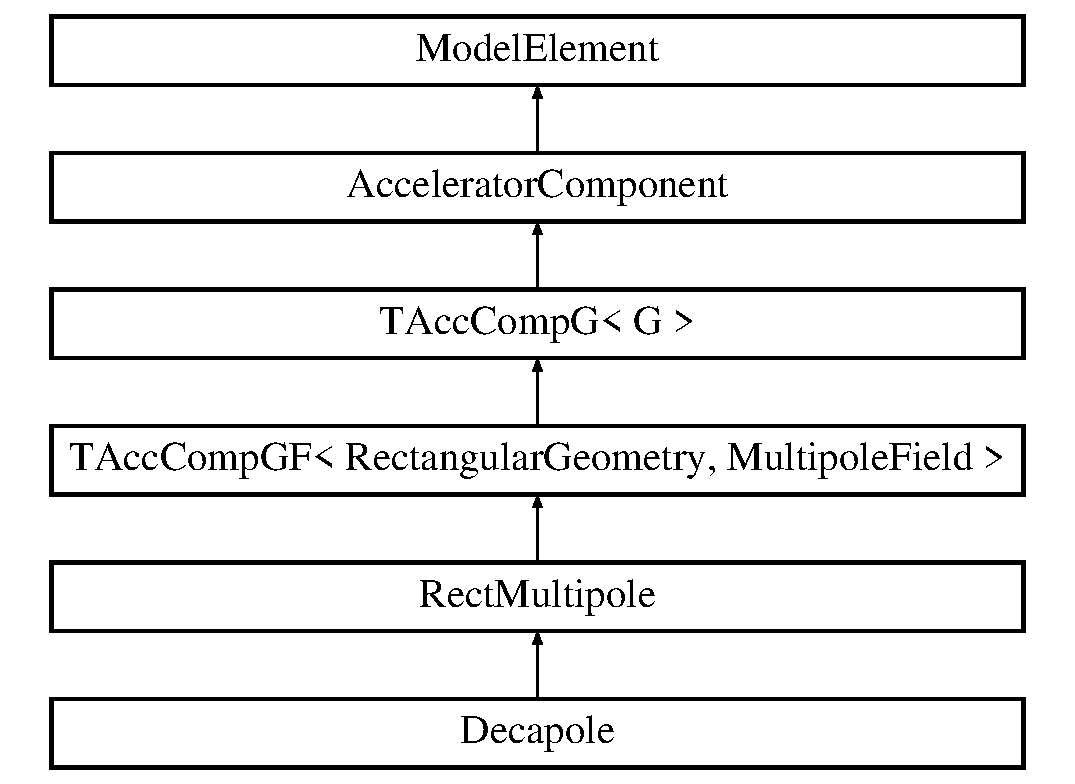
\includegraphics[height=6.000000cm]{classDecapole}
\end{center}
\end{figure}
\subsection*{Public Member Functions}
\begin{DoxyCompactItemize}
\item 
\mbox{\Hypertarget{classDecapole_aef67b36ade58a9fe117943cca2f4f4ef}\label{classDecapole_aef67b36ade58a9fe117943cca2f4f4ef}} 
{\bfseries Decapole} (const string \&\hyperlink{classModelElement_aada171ead2085c75b592cf07d91bc5c2}{id}, double len, double dnB)
\item 
\mbox{\Hypertarget{classDecapole_a7343a8e327da5d756edb2a1c69ebf591}\label{classDecapole_a7343a8e327da5d756edb2a1c69ebf591}} 
{\bfseries Decapole} (const string \&\hyperlink{classModelElement_aada171ead2085c75b592cf07d91bc5c2}{id}, double len, double B, double r0)
\item 
virtual void \hyperlink{classDecapole_a7fd7331bfbc39982539f8077afef2e6e}{Prepare\+Tracker} (\hyperlink{classComponentTracker}{Component\+Tracker} \&a\+Tracker)
\item 
virtual int \hyperlink{classDecapole_ac34dc3e11924c94ff4464cc0ca5ddf68}{Get\+Index} () const
\item 
virtual const string \& \hyperlink{classDecapole_af39bab6b0dd2177c83cc8dd548401103}{Get\+Type} () const
\item 
virtual \hyperlink{classModelElement}{Model\+Element} $\ast$ \hyperlink{classDecapole_a050b4c993227a975118da09b638ec450}{Copy} () const
\end{DoxyCompactItemize}
\subsection*{Static Public Attributes}
\begin{DoxyCompactItemize}
\item 
\mbox{\Hypertarget{classDecapole_a71ddf08cf9b2779f95cfc616763de2c8}\label{classDecapole_a71ddf08cf9b2779f95cfc616763de2c8}} 
static const int {\bfseries ID} = \hyperlink{classAcceleratorComponent_aa7ad4d39e1a488b705983842ed1ac784}{Unique\+Index}()
\end{DoxyCompactItemize}
\subsection*{Additional Inherited Members}


\subsection{Member Function Documentation}
\mbox{\Hypertarget{classDecapole_a050b4c993227a975118da09b638ec450}\label{classDecapole_a050b4c993227a975118da09b638ec450}} 
\index{Decapole@{Decapole}!Copy@{Copy}}
\index{Copy@{Copy}!Decapole@{Decapole}}
\subsubsection{\texorpdfstring{Copy()}{Copy()}}
{\footnotesize\ttfamily \hyperlink{classModelElement}{Model\+Element} $\ast$ Decapole\+::\+Copy (\begin{DoxyParamCaption}{ }\end{DoxyParamCaption}) const\hspace{0.3cm}{\ttfamily [virtual]}}

Virtual constructor. 

Implements \hyperlink{classModelElement_ac3ca26d649bd86a0f31a58ae09941429}{Model\+Element}.

\mbox{\Hypertarget{classDecapole_ac34dc3e11924c94ff4464cc0ca5ddf68}\label{classDecapole_ac34dc3e11924c94ff4464cc0ca5ddf68}} 
\index{Decapole@{Decapole}!Get\+Index@{Get\+Index}}
\index{Get\+Index@{Get\+Index}!Decapole@{Decapole}}
\subsubsection{\texorpdfstring{Get\+Index()}{GetIndex()}}
{\footnotesize\ttfamily int Decapole\+::\+Get\+Index (\begin{DoxyParamCaption}{ }\end{DoxyParamCaption}) const\hspace{0.3cm}{\ttfamily [virtual]}}

Returns the unique index for this class of accelerator components. \begin{DoxyReturn}{Returns}
An integer containing the unique index for this \hyperlink{classAcceleratorComponent}{Accelerator\+Component} type. 
\end{DoxyReturn}


Reimplemented from \hyperlink{classRectMultipole_a9bc789b2a193e341aab8bbd47a0e3ad4}{Rect\+Multipole}.

\mbox{\Hypertarget{classDecapole_af39bab6b0dd2177c83cc8dd548401103}\label{classDecapole_af39bab6b0dd2177c83cc8dd548401103}} 
\index{Decapole@{Decapole}!Get\+Type@{Get\+Type}}
\index{Get\+Type@{Get\+Type}!Decapole@{Decapole}}
\subsubsection{\texorpdfstring{Get\+Type()}{GetType()}}
{\footnotesize\ttfamily const string \& Decapole\+::\+Get\+Type (\begin{DoxyParamCaption}{ }\end{DoxyParamCaption}) const\hspace{0.3cm}{\ttfamily [virtual]}}

Return the type string for the element. \begin{DoxyReturn}{Returns}
A string containing the type of the element. 
\end{DoxyReturn}


Implements \hyperlink{classModelElement_a04dc2e51e1999fca612eb1838ec6b271}{Model\+Element}.

\mbox{\Hypertarget{classDecapole_a7fd7331bfbc39982539f8077afef2e6e}\label{classDecapole_a7fd7331bfbc39982539f8077afef2e6e}} 
\index{Decapole@{Decapole}!Prepare\+Tracker@{Prepare\+Tracker}}
\index{Prepare\+Tracker@{Prepare\+Tracker}!Decapole@{Decapole}}
\subsubsection{\texorpdfstring{Prepare\+Tracker()}{PrepareTracker()}}
{\footnotesize\ttfamily void Decapole\+::\+Prepare\+Tracker (\begin{DoxyParamCaption}\item[{\hyperlink{classComponentTracker}{Component\+Tracker} \&}]{a\+Tracker }\end{DoxyParamCaption})\hspace{0.3cm}{\ttfamily [virtual]}}

Primary tracking interface. Prepares the specified Tracker object for tracking this component. 
\begin{DoxyParams}[1]{Parameters}
\mbox{\tt in,out}  & {\em a\+Tracker} & The tracker to prepare. \\
\hline
\end{DoxyParams}


Reimplemented from \hyperlink{classRectMultipole_a2626d08254eee03cffb73abb20a9381a}{Rect\+Multipole}.



The documentation for this class was generated from the following files\+:\begin{DoxyCompactItemize}
\item 
/home/fallon/git/merlin-\/cmake/\+Merlin/Standard\+Multipoles.\+h\item 
/home/fallon/git/merlin-\/cmake/\+Merlin/Standard\+Multipoles.\+cpp\end{DoxyCompactItemize}

\hypertarget{classDefaultMarkerIntegrator}{}\section{Default\+Marker\+Integrator Class Reference}
\label{classDefaultMarkerIntegrator}\index{Default\+Marker\+Integrator@{Default\+Marker\+Integrator}}
Inheritance diagram for Default\+Marker\+Integrator\+:\begin{figure}[H]
\begin{center}
\leavevmode
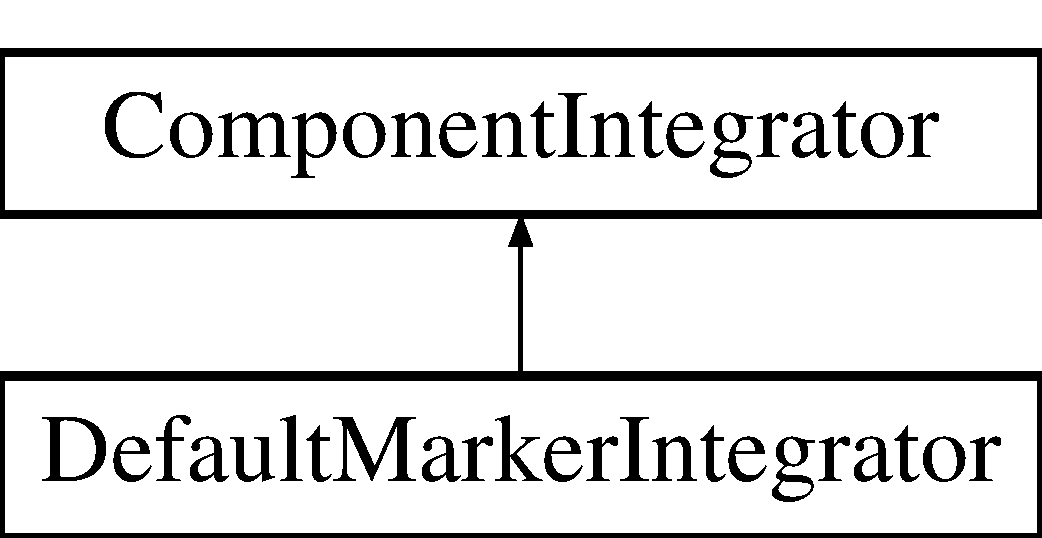
\includegraphics[height=2.000000cm]{classDefaultMarkerIntegrator}
\end{center}
\end{figure}
\subsection*{Public Member Functions}
\begin{DoxyCompactItemize}
\item 
\mbox{\Hypertarget{classDefaultMarkerIntegrator_a8b9a6a8fead23f02fa0996240ff63052}\label{classDefaultMarkerIntegrator_a8b9a6a8fead23f02fa0996240ff63052}} 
virtual void {\bfseries Track\+Step} (double ds)
\item 
\mbox{\Hypertarget{classDefaultMarkerIntegrator_a2e9df0ac86d3f001fafb89766ac594f7}\label{classDefaultMarkerIntegrator_a2e9df0ac86d3f001fafb89766ac594f7}} 
virtual int {\bfseries Get\+Component\+Index} () const
\end{DoxyCompactItemize}
\subsection*{Additional Inherited Members}


The documentation for this class was generated from the following file\+:\begin{DoxyCompactItemize}
\item 
/home/fallon/git/merlin-\/cmake/\+Merlin/Component\+Tracker.\+cpp\end{DoxyCompactItemize}

\hypertarget{structDeleteLatticeFunction}{}\section{Delete\+Lattice\+Function Struct Reference}
\label{structDeleteLatticeFunction}\index{Delete\+Lattice\+Function@{Delete\+Lattice\+Function}}
\subsection*{Public Member Functions}
\begin{DoxyCompactItemize}
\item 
\mbox{\Hypertarget{structDeleteLatticeFunction_a2a4dfdff879f293827c5704cfb42cc16}\label{structDeleteLatticeFunction_a2a4dfdff879f293827c5704cfb42cc16}} 
void {\bfseries operator()} (\hyperlink{classLatticeFunction}{Lattice\+Function} $\ast$lfn)
\end{DoxyCompactItemize}


The documentation for this struct was generated from the following file\+:\begin{DoxyCompactItemize}
\item 
/home/fallon/git/merlin-\/cmake/\+Merlin/Lattice\+Functions.\+cpp\end{DoxyCompactItemize}

\hypertarget{classdeleter}{}\section{deleter$<$ T $>$ Class Template Reference}
\label{classdeleter}\index{deleter$<$ T $>$@{deleter$<$ T $>$}}
\subsection*{Public Member Functions}
\begin{DoxyCompactItemize}
\item 
\mbox{\Hypertarget{classdeleter_a1f11e6dee735861e4391f150986bd8c0}\label{classdeleter_a1f11e6dee735861e4391f150986bd8c0}} 
void {\bfseries operator()} (T $\ast$p)
\end{DoxyCompactItemize}


The documentation for this class was generated from the following file\+:\begin{DoxyCompactItemize}
\item 
/home/fallon/git/merlin-\/cmake/\+Merlin/deleters.\+h\end{DoxyCompactItemize}

\hypertarget{classTLAS_1_1DimensionError}{}\section{T\+L\+AS\+:\+:Dimension\+Error Class Reference}
\label{classTLAS_1_1DimensionError}\index{T\+L\+A\+S\+::\+Dimension\+Error@{T\+L\+A\+S\+::\+Dimension\+Error}}


The documentation for this class was generated from the following file\+:\begin{DoxyCompactItemize}
\item 
/home/fallon/git/merlin-\/cmake/\+Merlin/T\+Matrix\+Lib.\+h\end{DoxyCompactItemize}

\hypertarget{classDiscreteUniform}{}\section{Discrete\+Uniform Class Reference}
\label{classDiscreteUniform}\index{Discrete\+Uniform@{Discrete\+Uniform}}
Inheritance diagram for Discrete\+Uniform\+:\begin{figure}[H]
\begin{center}
\leavevmode
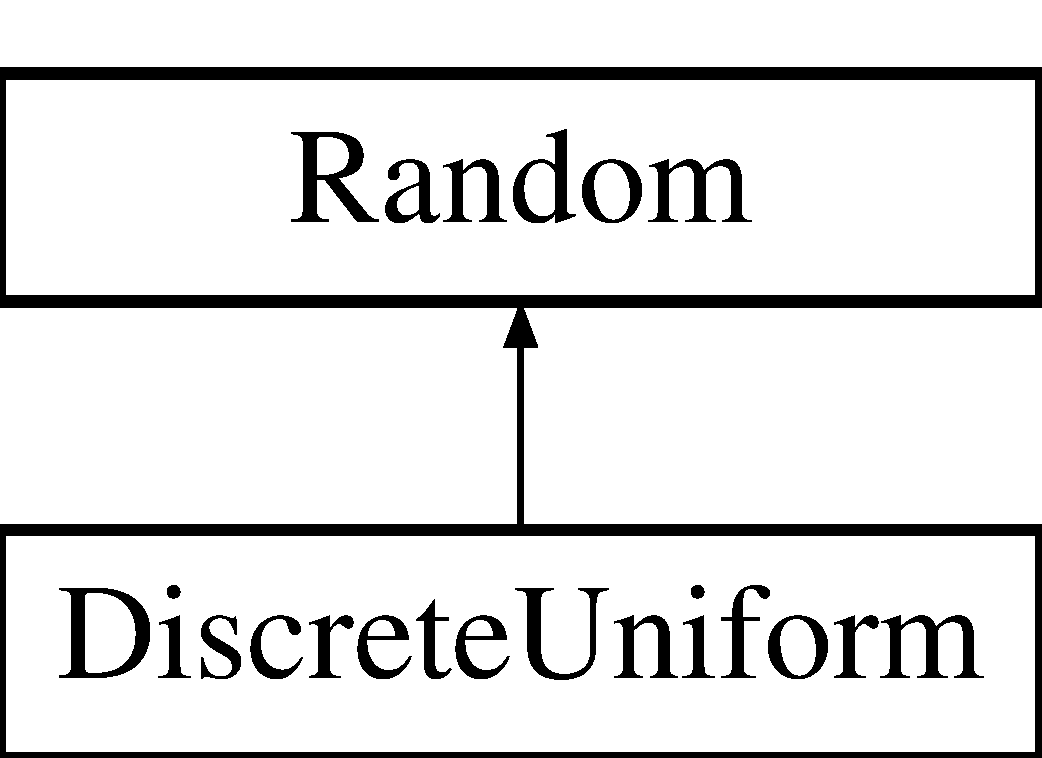
\includegraphics[height=2.000000cm]{classDiscreteUniform}
\end{center}
\end{figure}
\subsection*{Public Member Functions}
\begin{DoxyCompactItemize}
\item 
\mbox{\Hypertarget{classDiscreteUniform_a4cd644abbd479ee58e8b6bf70686db7a}\label{classDiscreteUniform_a4cd644abbd479ee58e8b6bf70686db7a}} 
{\bfseries Discrete\+Uniform} (long low, long high, \hyperlink{classRNG}{R\+NG} $\ast$gen)
\item 
\mbox{\Hypertarget{classDiscreteUniform_a68f6f2ad8c6c328e93e1585266034ad0}\label{classDiscreteUniform_a68f6f2ad8c6c328e93e1585266034ad0}} 
long {\bfseries low} ()
\item 
\mbox{\Hypertarget{classDiscreteUniform_a109761f3438d492cacd657c4b9aabaed}\label{classDiscreteUniform_a109761f3438d492cacd657c4b9aabaed}} 
long {\bfseries low} (long x)
\item 
\mbox{\Hypertarget{classDiscreteUniform_a7de12b0dfdda18803f90fe15d7449483}\label{classDiscreteUniform_a7de12b0dfdda18803f90fe15d7449483}} 
long {\bfseries high} ()
\item 
\mbox{\Hypertarget{classDiscreteUniform_adad3426a37c3e33d8619611994b164fd}\label{classDiscreteUniform_adad3426a37c3e33d8619611994b164fd}} 
long {\bfseries high} (long x)
\item 
\mbox{\Hypertarget{classDiscreteUniform_af10e3df9f920c1b3c9f77f1255c80494}\label{classDiscreteUniform_af10e3df9f920c1b3c9f77f1255c80494}} 
virtual double {\bfseries operator()} ()
\end{DoxyCompactItemize}
\subsection*{Additional Inherited Members}


The documentation for this class was generated from the following files\+:\begin{DoxyCompactItemize}
\item 
/home/fallon/git/merlin-\/cmake/\+Merlin/Disc\+Unif.\+h\item 
/home/fallon/git/merlin-\/cmake/\+Merlin/Disc\+Unif.\+cpp\end{DoxyCompactItemize}

\hypertarget{classDispersion}{}\section{Dispersion Class Reference}
\label{classDispersion}\index{Dispersion@{Dispersion}}
\subsection*{Public Member Functions}
\begin{DoxyCompactItemize}
\item 
\mbox{\Hypertarget{classDispersion_ada11ee98a456d0771489a38a7bbb5089}\label{classDispersion_ada11ee98a456d0771489a38a7bbb5089}} 
{\bfseries Dispersion} (\hyperlink{classAcceleratorModel}{Accelerator\+Model} $\ast$a\+Model, double ref\+Momentum)
\item 
\mbox{\Hypertarget{classDispersion_a38ddd6464b864201c419885427e6efcb}\label{classDispersion_a38ddd6464b864201c419885427e6efcb}} 
void {\bfseries Find\+Dispersion} (int n=0)
\item 
\mbox{\Hypertarget{classDispersion_a2c2dc96248506bffec89596a4c1e20e0}\label{classDispersion_a2c2dc96248506bffec89596a4c1e20e0}} 
void {\bfseries Find\+R\+M\+S\+Dispersion} (ofstream $\ast$file=nullptr)
\item 
\mbox{\Hypertarget{classDispersion_a89f3e942913a0ebb5364f2b0e542e228}\label{classDispersion_a89f3e942913a0ebb5364f2b0e542e228}} 
double {\bfseries Set\+Delta} (double new\+\_\+delta)
\end{DoxyCompactItemize}
\subsection*{Public Attributes}
\begin{DoxyCompactItemize}
\item 
\mbox{\Hypertarget{classDispersion_a59a3d8faa785ae15c685d7ee40c4e5ac}\label{classDispersion_a59a3d8faa785ae15c685d7ee40c4e5ac}} 
double {\bfseries Dx}
\item 
\mbox{\Hypertarget{classDispersion_a02e36e2131952e8f748235c5e6ff8169}\label{classDispersion_a02e36e2131952e8f748235c5e6ff8169}} 
double {\bfseries Dxp}
\item 
\mbox{\Hypertarget{classDispersion_a04b2faddfe2fd639bb66cf2f2d6476b4}\label{classDispersion_a04b2faddfe2fd639bb66cf2f2d6476b4}} 
double {\bfseries Dy}
\item 
\mbox{\Hypertarget{classDispersion_a14da8ca178ea8bcb5e856a6995078b87}\label{classDispersion_a14da8ca178ea8bcb5e856a6995078b87}} 
double {\bfseries Dyp}
\item 
\mbox{\Hypertarget{classDispersion_ab4fa7fd69dd9ec3b6356681ab05b8624}\label{classDispersion_ab4fa7fd69dd9ec3b6356681ab05b8624}} 
double {\bfseries Dx\+R\+MS}
\item 
\mbox{\Hypertarget{classDispersion_a80a1aeac15e980fed8a0d3aa4d1a6bd9}\label{classDispersion_a80a1aeac15e980fed8a0d3aa4d1a6bd9}} 
double {\bfseries Dy\+R\+MS}
\end{DoxyCompactItemize}


The documentation for this class was generated from the following files\+:\begin{DoxyCompactItemize}
\item 
/home/fallon/git/merlin-\/cmake/\+Merlin/Dispersion.\+h\item 
/home/fallon/git/merlin-\/cmake/\+Merlin/Dispersion.\+cpp\end{DoxyCompactItemize}

\hypertarget{classDrift}{}\section{Drift Class Reference}
\label{classDrift}\index{Drift@{Drift}}
Inheritance diagram for Drift\+:\begin{figure}[H]
\begin{center}
\leavevmode
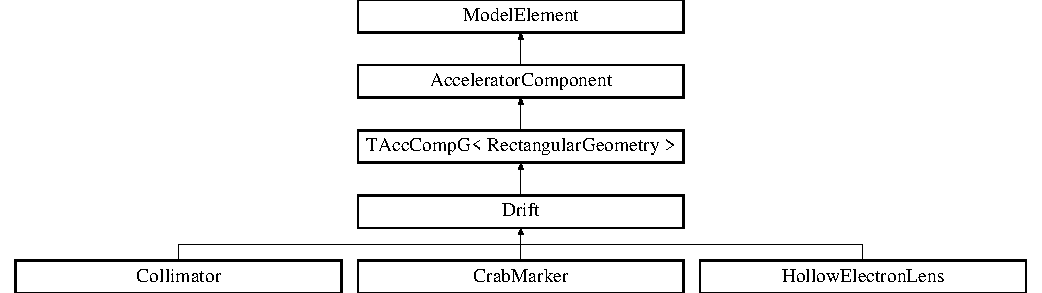
\includegraphics[height=3.938116cm]{classDrift}
\end{center}
\end{figure}
\subsection*{Public Member Functions}
\begin{DoxyCompactItemize}
\item 
\mbox{\Hypertarget{classDrift_a145d09c5783fcb458e9ee2269907fa5c}\label{classDrift_a145d09c5783fcb458e9ee2269907fa5c}} 
{\bfseries Drift} (const string \&\hyperlink{classModelElement_aada171ead2085c75b592cf07d91bc5c2}{id}, double len=0)
\item 
virtual const string \& \hyperlink{classDrift_a9f5e7d0aafd8689a4420b3d5e7b6879e}{Get\+Type} () const
\item 
virtual int \hyperlink{classDrift_a19bc19d48348912f8693e3ebbf9e92f2}{Get\+Index} () const
\item 
virtual void \hyperlink{classDrift_a9f3925549a0c7c99b39a1abea8546642}{Prepare\+Tracker} (\hyperlink{classComponentTracker}{Component\+Tracker} \&a\+Tracker)
\item 
virtual void \hyperlink{classDrift_abf387eddfcabfc81b186080f6301ce60}{Rotate\+Y180} ()
\item 
virtual \hyperlink{classModelElement}{Model\+Element} $\ast$ \hyperlink{classDrift_ae47df31297596e13944364d602c95ce5}{Copy} () const
\end{DoxyCompactItemize}
\subsection*{Static Public Attributes}
\begin{DoxyCompactItemize}
\item 
\mbox{\Hypertarget{classDrift_a885256e2c87bf0efc79b1295fd560a77}\label{classDrift_a885256e2c87bf0efc79b1295fd560a77}} 
static const int {\bfseries ID} = \hyperlink{classAcceleratorComponent_aa7ad4d39e1a488b705983842ed1ac784}{Unique\+Index}()
\end{DoxyCompactItemize}
\subsection*{Additional Inherited Members}


\subsection{Member Function Documentation}
\mbox{\Hypertarget{classDrift_ae47df31297596e13944364d602c95ce5}\label{classDrift_ae47df31297596e13944364d602c95ce5}} 
\index{Drift@{Drift}!Copy@{Copy}}
\index{Copy@{Copy}!Drift@{Drift}}
\subsubsection{\texorpdfstring{Copy()}{Copy()}}
{\footnotesize\ttfamily \hyperlink{classModelElement}{Model\+Element} $\ast$ Drift\+::\+Copy (\begin{DoxyParamCaption}{ }\end{DoxyParamCaption}) const\hspace{0.3cm}{\ttfamily [virtual]}}

Virtual constructor. 

Implements \hyperlink{classModelElement_ac3ca26d649bd86a0f31a58ae09941429}{Model\+Element}.



Reimplemented in \hyperlink{classCollimator_a82e63d47e1688d84f2e8f2fc3d247700}{Collimator}, \hyperlink{classHollowElectronLens_a95d48cbadab7dcc58a1d4c1d9895e8d3}{Hollow\+Electron\+Lens}, and \hyperlink{classCrabMarker_acd6d5d5a310e985f191443b42d8abc72}{Crab\+Marker}.

\mbox{\Hypertarget{classDrift_a19bc19d48348912f8693e3ebbf9e92f2}\label{classDrift_a19bc19d48348912f8693e3ebbf9e92f2}} 
\index{Drift@{Drift}!Get\+Index@{Get\+Index}}
\index{Get\+Index@{Get\+Index}!Drift@{Drift}}
\subsubsection{\texorpdfstring{Get\+Index()}{GetIndex()}}
{\footnotesize\ttfamily int Drift\+::\+Get\+Index (\begin{DoxyParamCaption}{ }\end{DoxyParamCaption}) const\hspace{0.3cm}{\ttfamily [virtual]}}

Returns the unique index for this class of accelerator components. \begin{DoxyReturn}{Returns}
An integer containing the unique index for this \hyperlink{classAcceleratorComponent}{Accelerator\+Component} type. 
\end{DoxyReturn}


Reimplemented from \hyperlink{classAcceleratorComponent_abd1490171ac9af6004d3da01fb3b95fb}{Accelerator\+Component}.



Reimplemented in \hyperlink{classCollimator_a158a9d8999d55a27efe4e56e5af8b56a}{Collimator}, \hyperlink{classHollowElectronLens_a87c06909a695e81cb1abc546019e4e40}{Hollow\+Electron\+Lens}, and \hyperlink{classCrabMarker_ae8678c41613db9792f84faf3feb88f2b}{Crab\+Marker}.

\mbox{\Hypertarget{classDrift_a9f5e7d0aafd8689a4420b3d5e7b6879e}\label{classDrift_a9f5e7d0aafd8689a4420b3d5e7b6879e}} 
\index{Drift@{Drift}!Get\+Type@{Get\+Type}}
\index{Get\+Type@{Get\+Type}!Drift@{Drift}}
\subsubsection{\texorpdfstring{Get\+Type()}{GetType()}}
{\footnotesize\ttfamily const string \& Drift\+::\+Get\+Type (\begin{DoxyParamCaption}{ }\end{DoxyParamCaption}) const\hspace{0.3cm}{\ttfamily [virtual]}}

Return the type string for the element. \begin{DoxyReturn}{Returns}
A string containing the type of the element. 
\end{DoxyReturn}


Implements \hyperlink{classModelElement_a04dc2e51e1999fca612eb1838ec6b271}{Model\+Element}.



Reimplemented in \hyperlink{classCollimator_aab811743031565147b965ca9b9fdfbc4}{Collimator}, \hyperlink{classHollowElectronLens_add07b8f08bad11edfb3df87be488e9ff}{Hollow\+Electron\+Lens}, and \hyperlink{classCrabMarker_a45ab65449808d5072eb033858c2d961a}{Crab\+Marker}.

\mbox{\Hypertarget{classDrift_a9f3925549a0c7c99b39a1abea8546642}\label{classDrift_a9f3925549a0c7c99b39a1abea8546642}} 
\index{Drift@{Drift}!Prepare\+Tracker@{Prepare\+Tracker}}
\index{Prepare\+Tracker@{Prepare\+Tracker}!Drift@{Drift}}
\subsubsection{\texorpdfstring{Prepare\+Tracker()}{PrepareTracker()}}
{\footnotesize\ttfamily void Drift\+::\+Prepare\+Tracker (\begin{DoxyParamCaption}\item[{\hyperlink{classComponentTracker}{Component\+Tracker} \&}]{a\+Tracker }\end{DoxyParamCaption})\hspace{0.3cm}{\ttfamily [virtual]}}

Primary tracking interface. Prepares the specified Tracker object for tracking this component. 
\begin{DoxyParams}[1]{Parameters}
\mbox{\tt in,out}  & {\em a\+Tracker} & The tracker to prepare. \\
\hline
\end{DoxyParams}


Reimplemented from \hyperlink{classAcceleratorComponent_ab897c54689ac946f40c3ad0716ddd4bb}{Accelerator\+Component}.



Reimplemented in \hyperlink{classCollimator_acbcf691bfcf53d652d14b9381c711fe7}{Collimator}, \hyperlink{classHollowElectronLens_a86e8e69936f636a5d3fa0675e0434bf4}{Hollow\+Electron\+Lens}, and \hyperlink{classCrabMarker_ab29822625603a198dc7623979ed1bb3b}{Crab\+Marker}.

\mbox{\Hypertarget{classDrift_abf387eddfcabfc81b186080f6301ce60}\label{classDrift_abf387eddfcabfc81b186080f6301ce60}} 
\index{Drift@{Drift}!Rotate\+Y180@{Rotate\+Y180}}
\index{Rotate\+Y180@{Rotate\+Y180}!Drift@{Drift}}
\subsubsection{\texorpdfstring{Rotate\+Y180()}{RotateY180()}}
{\footnotesize\ttfamily void Drift\+::\+Rotate\+Y180 (\begin{DoxyParamCaption}{ }\end{DoxyParamCaption})\hspace{0.3cm}{\ttfamily [virtual]}}

Rotates the component 180 degrees about its local Y axis. 

Implements \hyperlink{classAcceleratorComponent_a8bf0d39b56578ca99f286ca1504b9072}{Accelerator\+Component}.



Reimplemented in \hyperlink{classCollimator_a89d782779f8e57af28eeb963078bbf20}{Collimator}, \hyperlink{classHollowElectronLens_a8e806750ac6f8129d3be4a089303da36}{Hollow\+Electron\+Lens}, and \hyperlink{classCrabMarker_a4b60620517f65b4e1f557300a3dbe89b}{Crab\+Marker}.



The documentation for this class was generated from the following files\+:\begin{DoxyCompactItemize}
\item 
/home/fallon/git/merlin-\/cmake/\+Merlin/Drift.\+h\item 
/home/fallon/git/merlin-\/cmake/\+Merlin/Drift.\+cpp\end{DoxyCompactItemize}

\hypertarget{classSMPTracking_1_1DriftCI}{}\section{S\+M\+P\+Tracking\+:\+:Drift\+CI Class Reference}
\label{classSMPTracking_1_1DriftCI}\index{S\+M\+P\+Tracking\+::\+Drift\+CI@{S\+M\+P\+Tracking\+::\+Drift\+CI}}
Inheritance diagram for S\+M\+P\+Tracking\+:\+:Drift\+CI\+:\begin{figure}[H]
\begin{center}
\leavevmode
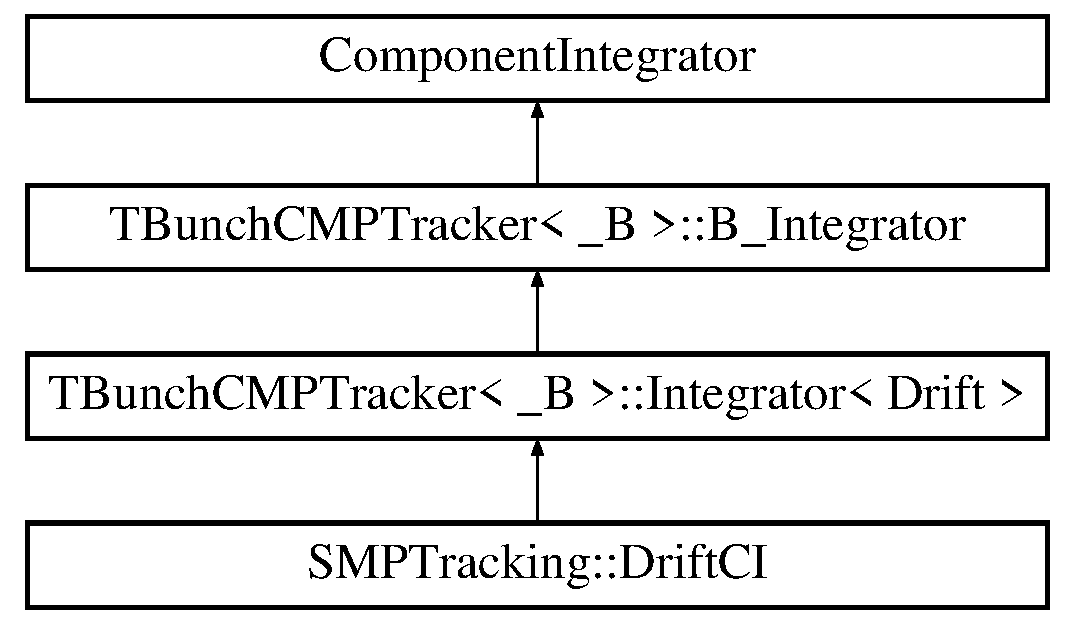
\includegraphics[height=4.000000cm]{classSMPTracking_1_1DriftCI}
\end{center}
\end{figure}
\subsection*{Protected Member Functions}
\begin{DoxyCompactItemize}
\item 
\mbox{\Hypertarget{classSMPTracking_1_1DriftCI_a03279e4909b380097b10de4ab97dc39c}\label{classSMPTracking_1_1DriftCI_a03279e4909b380097b10de4ab97dc39c}} 
void {\bfseries Track\+Step} (double ds)
\end{DoxyCompactItemize}
\subsection*{Additional Inherited Members}


The documentation for this class was generated from the following files\+:\begin{DoxyCompactItemize}
\item 
/home/fallon/git/merlin-\/cmake/\+Merlin/S\+M\+P\+Std\+Integrators.\+h\item 
/home/fallon/git/merlin-\/cmake/\+Merlin/S\+M\+P\+Std\+Integrators.\+cpp\item 
/home/fallon/git/merlin-\/cmake/\+Merlin/Std\+Integrators.\+cpp\item 
/home/fallon/git/merlin-\/cmake/\+Merlin/Symplectic\+Integrators.\+cpp\end{DoxyCompactItemize}

\hypertarget{structParticleTracking_1_1DriftMap}{}\section{Particle\+Tracking\+:\+:Drift\+Map Struct Reference}
\label{structParticleTracking_1_1DriftMap}\index{Particle\+Tracking\+::\+Drift\+Map@{Particle\+Tracking\+::\+Drift\+Map}}
\subsection*{Public Member Functions}
\begin{DoxyCompactItemize}
\item 
\mbox{\Hypertarget{structParticleTracking_1_1DriftMap_ae8a4b596efe78885579de4aebecbc9a2}\label{structParticleTracking_1_1DriftMap_ae8a4b596efe78885579de4aebecbc9a2}} 
{\bfseries Drift\+Map} (double l)
\item 
\mbox{\Hypertarget{structParticleTracking_1_1DriftMap_a88e2c1d56ebeaf11fe0d8507ad07e48d}\label{structParticleTracking_1_1DriftMap_a88e2c1d56ebeaf11fe0d8507ad07e48d}} 
void {\bfseries Apply} (\hyperlink{classPSvector}{P\+Svector} \&x) const
\end{DoxyCompactItemize}
\subsection*{Public Attributes}
\begin{DoxyCompactItemize}
\item 
\mbox{\Hypertarget{structParticleTracking_1_1DriftMap_a0d11b751191b5bb65c8a3303ed479e1f}\label{structParticleTracking_1_1DriftMap_a0d11b751191b5bb65c8a3303ed479e1f}} 
double {\bfseries s}
\end{DoxyCompactItemize}


The documentation for this struct was generated from the following file\+:\begin{DoxyCompactItemize}
\item 
/home/fallon/git/merlin-\/cmake/\+Merlin/L\+C\+A\+Vintegrator.\+cpp\end{DoxyCompactItemize}

\hypertarget{structParticleTracking_1_1SYMPLECTIC_1_1DriftMap}{}\section{Particle\+Tracking\+:\+:S\+Y\+M\+P\+L\+E\+C\+T\+IC\+:\+:Drift\+Map Struct Reference}
\label{structParticleTracking_1_1SYMPLECTIC_1_1DriftMap}\index{Particle\+Tracking\+::\+S\+Y\+M\+P\+L\+E\+C\+T\+I\+C\+::\+Drift\+Map@{Particle\+Tracking\+::\+S\+Y\+M\+P\+L\+E\+C\+T\+I\+C\+::\+Drift\+Map}}
\subsection*{Public Member Functions}
\begin{DoxyCompactItemize}
\item 
\mbox{\Hypertarget{structParticleTracking_1_1SYMPLECTIC_1_1DriftMap_a80b6ab7ccd49226e6badf3e54180d3a8}\label{structParticleTracking_1_1SYMPLECTIC_1_1DriftMap_a80b6ab7ccd49226e6badf3e54180d3a8}} 
{\bfseries Drift\+Map} (double \+\_\+ds)
\item 
\mbox{\Hypertarget{structParticleTracking_1_1SYMPLECTIC_1_1DriftMap_ac7126df37adc5bb08d4e1fbc6165e425}\label{structParticleTracking_1_1SYMPLECTIC_1_1DriftMap_ac7126df37adc5bb08d4e1fbc6165e425}} 
void {\bfseries operator()} (\hyperlink{classPSvector}{P\+Svector} \&v) const
\end{DoxyCompactItemize}


The documentation for this struct was generated from the following file\+:\begin{DoxyCompactItemize}
\item 
/home/fallon/git/merlin-\/cmake/\+Merlin/Symplectic\+Integrators.\+cpp\end{DoxyCompactItemize}

\hypertarget{classbasic__echo__ostream_1_1echo__streambuf}{}\section{basic\+\_\+echo\+\_\+ostream$<$ T, Tr $>$\+:\+:echo\+\_\+streambuf Class Reference}
\label{classbasic__echo__ostream_1_1echo__streambuf}\index{basic\+\_\+echo\+\_\+ostream$<$ T, Tr $>$\+::echo\+\_\+streambuf@{basic\+\_\+echo\+\_\+ostream$<$ T, Tr $>$\+::echo\+\_\+streambuf}}
Inheritance diagram for basic\+\_\+echo\+\_\+ostream$<$ T, Tr $>$\+:\+:echo\+\_\+streambuf\+:\begin{figure}[H]
\begin{center}
\leavevmode
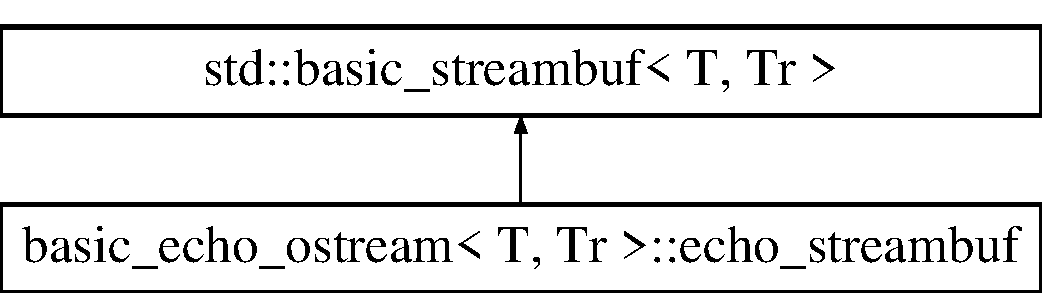
\includegraphics[height=2.000000cm]{classbasic__echo__ostream_1_1echo__streambuf}
\end{center}
\end{figure}
\subsection*{Public Member Functions}
\begin{DoxyCompactItemize}
\item 
\mbox{\Hypertarget{classbasic__echo__ostream_1_1echo__streambuf_a6786d570d7a3c2d1b5846b89bfb5bac6}\label{classbasic__echo__ostream_1_1echo__streambuf_a6786d570d7a3c2d1b5846b89bfb5bac6}} 
{\bfseries echo\+\_\+streambuf} (std\+::basic\+\_\+ostream$<$ T, Tr $>$ \&os1, std\+::basic\+\_\+ostream$<$ T, Tr $>$ \&os2)
\end{DoxyCompactItemize}
\subsection*{Protected Member Functions}
\begin{DoxyCompactItemize}
\item 
\mbox{\Hypertarget{classbasic__echo__ostream_1_1echo__streambuf_a3940a28cc68fab9e66aee12856537972}\label{classbasic__echo__ostream_1_1echo__streambuf_a3940a28cc68fab9e66aee12856537972}} 
virtual int\+\_\+type {\bfseries overflow} (int\+\_\+type c)
\end{DoxyCompactItemize}


The documentation for this class was generated from the following file\+:\begin{DoxyCompactItemize}
\item 
/home/fallon/git/merlin-\/cmake/\+Merlin/echo\+\_\+ostream.\+h\end{DoxyCompactItemize}

\hypertarget{classCollimation_1_1Elasticpn}{}\section{Collimation\+:\+:Elasticpn Class Reference}
\label{classCollimation_1_1Elasticpn}\index{Collimation\+::\+Elasticpn@{Collimation\+::\+Elasticpn}}
Inheritance diagram for Collimation\+:\+:Elasticpn\+:\begin{figure}[H]
\begin{center}
\leavevmode
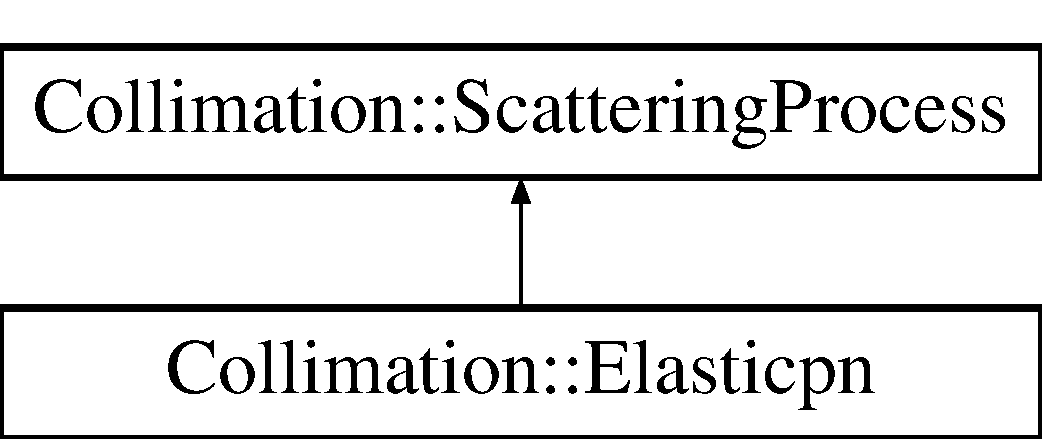
\includegraphics[height=2.000000cm]{classCollimation_1_1Elasticpn}
\end{center}
\end{figure}
\subsection*{Public Member Functions}
\begin{DoxyCompactItemize}
\item 
\mbox{\Hypertarget{classCollimation_1_1Elasticpn_a4936dc72ce59bf97e08d7b3d08a04f4e}\label{classCollimation_1_1Elasticpn_a4936dc72ce59bf97e08d7b3d08a04f4e}} 
void {\bfseries Configure} (\hyperlink{classMaterial}{Material} $\ast$matin, \hyperlink{classCollimation_1_1CrossSections}{Cross\+Sections} $\ast$C\+Sin)
\item 
\mbox{\Hypertarget{classCollimation_1_1Elasticpn_aad8b618c7a11d3deebae1d367e094d0a}\label{classCollimation_1_1Elasticpn_aad8b618c7a11d3deebae1d367e094d0a}} 
bool {\bfseries Scatter} (\hyperlink{classPSvector}{P\+Svector} \&p, double E)
\item 
\mbox{\Hypertarget{classCollimation_1_1Elasticpn_ad2113716a36e2f4b35763044726122ec}\label{classCollimation_1_1Elasticpn_ad2113716a36e2f4b35763044726122ec}} 
std\+::string {\bfseries Get\+Process\+Type} () const
\end{DoxyCompactItemize}
\subsection*{Additional Inherited Members}


The documentation for this class was generated from the following files\+:\begin{DoxyCompactItemize}
\item 
/home/fallon/git/merlin-\/cmake/\+Merlin/Scattering\+Process.\+h\item 
/home/fallon/git/merlin-\/cmake/\+Merlin/Scattering\+Process.\+cpp\end{DoxyCompactItemize}

\hypertarget{classCollimation_1_1ElasticpN}{}\section{Collimation\+:\+:ElasticpN Class Reference}
\label{classCollimation_1_1ElasticpN}\index{Collimation\+::\+ElasticpN@{Collimation\+::\+ElasticpN}}
Inheritance diagram for Collimation\+:\+:ElasticpN\+:\begin{figure}[H]
\begin{center}
\leavevmode
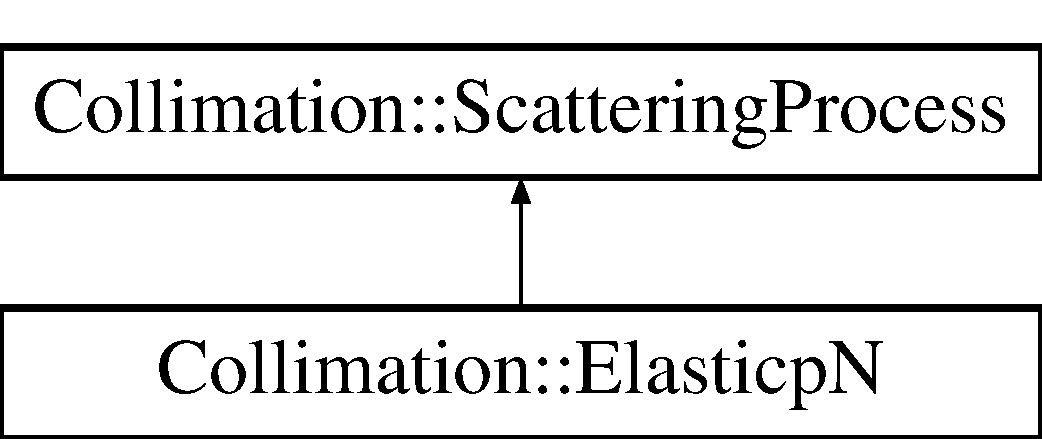
\includegraphics[height=2.000000cm]{classCollimation_1_1ElasticpN}
\end{center}
\end{figure}
\subsection*{Public Member Functions}
\begin{DoxyCompactItemize}
\item 
\mbox{\Hypertarget{classCollimation_1_1ElasticpN_accb8e381e0c880d0b4c6fa62d98c83c4}\label{classCollimation_1_1ElasticpN_accb8e381e0c880d0b4c6fa62d98c83c4}} 
void {\bfseries Configure} (\hyperlink{classMaterial}{Material} $\ast$matin, \hyperlink{classCollimation_1_1CrossSections}{Cross\+Sections} $\ast$C\+Sin)
\item 
\mbox{\Hypertarget{classCollimation_1_1ElasticpN_a8b912ff2801930f895ae26ad03e356d6}\label{classCollimation_1_1ElasticpN_a8b912ff2801930f895ae26ad03e356d6}} 
bool {\bfseries Scatter} (\hyperlink{classPSvector}{P\+Svector} \&p, double E)
\item 
\mbox{\Hypertarget{classCollimation_1_1ElasticpN_ae6850b1195f075ba5115e02acdb72e27}\label{classCollimation_1_1ElasticpN_ae6850b1195f075ba5115e02acdb72e27}} 
std\+::string {\bfseries Get\+Process\+Type} () const
\end{DoxyCompactItemize}
\subsection*{Additional Inherited Members}


The documentation for this class was generated from the following files\+:\begin{DoxyCompactItemize}
\item 
/home/fallon/git/merlin-\/cmake/\+Merlin/Scattering\+Process.\+h\item 
/home/fallon/git/merlin-\/cmake/\+Merlin/Scattering\+Process.\+cpp\end{DoxyCompactItemize}

\hypertarget{classParticleTracking_1_1ElectronBunch}{}\section{Particle\+Tracking\+:\+:Electron\+Bunch Class Reference}
\label{classParticleTracking_1_1ElectronBunch}\index{Particle\+Tracking\+::\+Electron\+Bunch@{Particle\+Tracking\+::\+Electron\+Bunch}}
Inheritance diagram for Particle\+Tracking\+:\+:Electron\+Bunch\+:\begin{figure}[H]
\begin{center}
\leavevmode
\includegraphics[height=4.000000cm]{classParticleTracking_1_1ElectronBunch}
\end{center}
\end{figure}
\subsection*{Public Member Functions}
\begin{DoxyCompactItemize}
\item 
\mbox{\Hypertarget{classParticleTracking_1_1ElectronBunch_a3ece7133ea022eadf059234b38318b63}\label{classParticleTracking_1_1ElectronBunch_a3ece7133ea022eadf059234b38318b63}} 
{\bfseries Electron\+Bunch} (double P0, double \hyperlink{namespaceParticleTracking_a3e89510a540596b235a808915deb0f7a}{Q}, P\+Svector\+Array \&particles)
\item 
\mbox{\Hypertarget{classParticleTracking_1_1ElectronBunch_a614833e3c43033b193c361cfa0c67c9b}\label{classParticleTracking_1_1ElectronBunch_a614833e3c43033b193c361cfa0c67c9b}} 
{\bfseries Electron\+Bunch} (double P0, double \hyperlink{namespaceParticleTracking_a3e89510a540596b235a808915deb0f7a}{Q}, std\+::istream \&is)
\item 
\mbox{\Hypertarget{classParticleTracking_1_1ElectronBunch_acba0ccc138b89bd959cccb553917e975}\label{classParticleTracking_1_1ElectronBunch_acba0ccc138b89bd959cccb553917e975}} 
{\bfseries Electron\+Bunch} (double P0, double Qm=1)
\item 
\mbox{\Hypertarget{classParticleTracking_1_1ElectronBunch_ade1b916df46d59543b8023e94bff1b01}\label{classParticleTracking_1_1ElectronBunch_ade1b916df46d59543b8023e94bff1b01}} 
virtual bool {\bfseries Is\+Stable} () const
\item 
\mbox{\Hypertarget{classParticleTracking_1_1ElectronBunch_a2dcf33728949051ac3a3213636bbadbc}\label{classParticleTracking_1_1ElectronBunch_a2dcf33728949051ac3a3213636bbadbc}} 
virtual double {\bfseries Get\+Particle\+Mass} () const
\item 
\mbox{\Hypertarget{classParticleTracking_1_1ElectronBunch_aa2fb3184a2f3a43b15c718ca1b6c76a3}\label{classParticleTracking_1_1ElectronBunch_aa2fb3184a2f3a43b15c718ca1b6c76a3}} 
virtual double {\bfseries Get\+Particle\+Mass\+MeV} () const
\item 
\mbox{\Hypertarget{classParticleTracking_1_1ElectronBunch_a28065187be47dd9c62cfa9711897d6d7}\label{classParticleTracking_1_1ElectronBunch_a28065187be47dd9c62cfa9711897d6d7}} 
virtual double {\bfseries Get\+Particle\+Lifetime} () const
\item 
\mbox{\Hypertarget{classParticleTracking_1_1ElectronBunch_aa7a7b711f90f558030b9c69949ab668e}\label{classParticleTracking_1_1ElectronBunch_aa7a7b711f90f558030b9c69949ab668e}} 
void {\bfseries set} ()
\item 
\mbox{\Hypertarget{classParticleTracking_1_1ElectronBunch_aa253bb32fb5041946c43002ae4e9d736}\label{classParticleTracking_1_1ElectronBunch_aa253bb32fb5041946c43002ae4e9d736}} 
void {\bfseries report} ()
\end{DoxyCompactItemize}
\subsection*{Additional Inherited Members}


The documentation for this class was generated from the following files\+:\begin{DoxyCompactItemize}
\item 
/home/fallon/git/merlin-\/cmake/\+Merlin/Electron\+Bunch.\+h\item 
/home/fallon/git/merlin-\/cmake/\+Merlin/Electron\+Bunch.\+cpp\end{DoxyCompactItemize}

\hypertarget{classElementRepository}{}\section{Element\+Repository Class Reference}
\label{classElementRepository}\index{Element\+Repository@{Element\+Repository}}
\subsection*{Public Types}
\begin{DoxyCompactItemize}
\item 
\mbox{\Hypertarget{classElementRepository_aa336fe6741b21762f5e0f28311ff24a6}\label{classElementRepository_aa336fe6741b21762f5e0f28311ff24a6}} 
typedef std\+::set$<$ \hyperlink{classModelElement}{Model\+Element} $\ast$$>$ {\bfseries Element\+Set}
\item 
\mbox{\Hypertarget{classElementRepository_a789e7a8685d8e44d0fd3fe8a80d2d45f}\label{classElementRepository_a789e7a8685d8e44d0fd3fe8a80d2d45f}} 
typedef Element\+Set\+::iterator {\bfseries iterator}
\item 
\mbox{\Hypertarget{classElementRepository_a7ac8b068862b2ce832973594fd47599a}\label{classElementRepository_a7ac8b068862b2ce832973594fd47599a}} 
typedef Element\+Set\+::const\+\_\+iterator {\bfseries const\+\_\+iterator}
\end{DoxyCompactItemize}
\subsection*{Public Member Functions}
\begin{DoxyCompactItemize}
\item 
\mbox{\Hypertarget{classElementRepository_a5c7dee409a53d501144a9cf5c6200e1e}\label{classElementRepository_a5c7dee409a53d501144a9cf5c6200e1e}} 
bool {\bfseries Add} (\hyperlink{classModelElement}{Model\+Element} $\ast$an\+Element)
\item 
\mbox{\Hypertarget{classElementRepository_a48528e41abe5ed8a121db383ead83f63}\label{classElementRepository_a48528e41abe5ed8a121db383ead83f63}} 
size\+\_\+t {\bfseries Count} (const std\+::string \&id) const
\item 
\mbox{\Hypertarget{classElementRepository_ae8833698c1c4efa1fffd01547d9166dd}\label{classElementRepository_ae8833698c1c4efa1fffd01547d9166dd}} 
size\+\_\+t {\bfseries Find} (const std\+::string \&id, std\+::vector$<$ \hyperlink{classModelElement}{Model\+Element} $\ast$$>$ \&elements)
\item 
\mbox{\Hypertarget{classElementRepository_a3fc873824d592ab3a60964de5f32691f}\label{classElementRepository_a3fc873824d592ab3a60964de5f32691f}} 
size\+\_\+t {\bfseries Size} () const
\item 
\mbox{\Hypertarget{classElementRepository_a064256ae32d76ad39d96c931ab672b84}\label{classElementRepository_a064256ae32d76ad39d96c931ab672b84}} 
Element\+Repository\+::iterator {\bfseries begin} ()
\item 
\mbox{\Hypertarget{classElementRepository_a486611a7bbecfa3af43d21e8193eb8f9}\label{classElementRepository_a486611a7bbecfa3af43d21e8193eb8f9}} 
Element\+Repository\+::iterator {\bfseries end} ()
\item 
\mbox{\Hypertarget{classElementRepository_afd781833fb84125ff0ece3174785b554}\label{classElementRepository_afd781833fb84125ff0ece3174785b554}} 
Element\+Repository\+::const\+\_\+iterator {\bfseries begin} () const
\item 
\mbox{\Hypertarget{classElementRepository_ae5268cb7a343889091f8fb4eccab2403}\label{classElementRepository_ae5268cb7a343889091f8fb4eccab2403}} 
Element\+Repository\+::const\+\_\+iterator {\bfseries end} () const
\end{DoxyCompactItemize}
\subsection*{Public Attributes}
\begin{DoxyCompactItemize}
\item 
\mbox{\Hypertarget{classElementRepository_a091e41cbcced653eb54c59531e0db8fa}\label{classElementRepository_a091e41cbcced653eb54c59531e0db8fa}} 
Element\+Set {\bfseries the\+Elements}
\end{DoxyCompactItemize}


The documentation for this class was generated from the following files\+:\begin{DoxyCompactItemize}
\item 
/home/fallon/git/merlin-\/cmake/\+Merlin/Element\+Repository.\+h\item 
/home/fallon/git/merlin-\/cmake/\+Merlin/Element\+Repository.\+cpp\end{DoxyCompactItemize}

\hypertarget{classEllipticalAperture}{}\section{Elliptical\+Aperture Class Reference}
\label{classEllipticalAperture}\index{Elliptical\+Aperture@{Elliptical\+Aperture}}


{\ttfamily \#include $<$Simple\+Apertures.\+h$>$}

Inheritance diagram for Elliptical\+Aperture\+:\begin{figure}[H]
\begin{center}
\leavevmode
\includegraphics[height=2.000000cm]{classEllipticalAperture}
\end{center}
\end{figure}
\subsection*{Public Member Functions}
\begin{DoxyCompactItemize}
\item 
\mbox{\Hypertarget{classEllipticalAperture_a4eed40d814a493a2260d0db04c8cf663}\label{classEllipticalAperture_a4eed40d814a493a2260d0db04c8cf663}} 
{\bfseries Elliptical\+Aperture} (double width, double height)
\item 
\mbox{\Hypertarget{classEllipticalAperture_a1552d434f593fc0c9ea91ef2c958f533}\label{classEllipticalAperture_a1552d434f593fc0c9ea91ef2c958f533}} 
double {\bfseries Get\+Half\+Width} () const
\item 
\mbox{\Hypertarget{classEllipticalAperture_a86aa77eab0fb05163f178ebcdb4f4bed}\label{classEllipticalAperture_a86aa77eab0fb05163f178ebcdb4f4bed}} 
double {\bfseries Get\+Half\+Height} () const
\item 
virtual bool \hyperlink{classEllipticalAperture_ad2ac194f4f03d5e590a7640afa69ace9}{Point\+Inside} (double x, double y, double z) const
\item 
virtual double \hyperlink{classEllipticalAperture_aec41ce72d82e004b8de123e37d3b11e9}{Get\+Radius\+At} (double phi, double z) const
\item 
virtual std\+::string \hyperlink{classEllipticalAperture_a8c56e3ab5e8483dd42ed6e35855409df}{Get\+Aperture\+Type} () const
\item 
virtual void \hyperlink{classEllipticalAperture_af45343465b84072027de770839bbd73d}{printout} (std\+::ostream \&out) const
\end{DoxyCompactItemize}
\subsection*{Additional Inherited Members}


\subsection{Detailed Description}
Represents an aperture with an elliptical cross-\/section. The aperture is assumed extruded along its geometry. 

\subsection{Member Function Documentation}
\mbox{\Hypertarget{classEllipticalAperture_a8c56e3ab5e8483dd42ed6e35855409df}\label{classEllipticalAperture_a8c56e3ab5e8483dd42ed6e35855409df}} 
\index{Elliptical\+Aperture@{Elliptical\+Aperture}!Get\+Aperture\+Type@{Get\+Aperture\+Type}}
\index{Get\+Aperture\+Type@{Get\+Aperture\+Type}!Elliptical\+Aperture@{Elliptical\+Aperture}}
\subsubsection{\texorpdfstring{Get\+Aperture\+Type()}{GetApertureType()}}
{\footnotesize\ttfamily std\+::string Elliptical\+Aperture\+::\+Get\+Aperture\+Type (\begin{DoxyParamCaption}{ }\end{DoxyParamCaption}) const\hspace{0.3cm}{\ttfamily [inline]}, {\ttfamily [virtual]}}

Returns the type of the aperture. \begin{DoxyReturn}{Returns}
A string containing the type of the aperture. 
\end{DoxyReturn}


Implements \hyperlink{classAperture_ad7af612271a0586feea83c38549dfb75}{Aperture}.

\mbox{\Hypertarget{classEllipticalAperture_aec41ce72d82e004b8de123e37d3b11e9}\label{classEllipticalAperture_aec41ce72d82e004b8de123e37d3b11e9}} 
\index{Elliptical\+Aperture@{Elliptical\+Aperture}!Get\+Radius\+At@{Get\+Radius\+At}}
\index{Get\+Radius\+At@{Get\+Radius\+At}!Elliptical\+Aperture@{Elliptical\+Aperture}}
\subsubsection{\texorpdfstring{Get\+Radius\+At()}{GetRadiusAt()}}
{\footnotesize\ttfamily double Elliptical\+Aperture\+::\+Get\+Radius\+At (\begin{DoxyParamCaption}\item[{double}]{phi,  }\item[{double}]{z }\end{DoxyParamCaption}) const\hspace{0.3cm}{\ttfamily [virtual]}}

Returns the radius to the aperture at the angle phi. The z coordinate is ignored.

Elliptical \hyperlink{classAperture}{Aperture} Functions 

Implements \hyperlink{classAperture_ad0ea7907d393ec1e6a8303343fe9dd29}{Aperture}.

\mbox{\Hypertarget{classEllipticalAperture_ad2ac194f4f03d5e590a7640afa69ace9}\label{classEllipticalAperture_ad2ac194f4f03d5e590a7640afa69ace9}} 
\index{Elliptical\+Aperture@{Elliptical\+Aperture}!Point\+Inside@{Point\+Inside}}
\index{Point\+Inside@{Point\+Inside}!Elliptical\+Aperture@{Elliptical\+Aperture}}
\subsubsection{\texorpdfstring{Point\+Inside()}{PointInside()}}
{\footnotesize\ttfamily bool Elliptical\+Aperture\+::\+Point\+Inside (\begin{DoxyParamCaption}\item[{double}]{x,  }\item[{double}]{y,  }\item[{double}]{z }\end{DoxyParamCaption}) const\hspace{0.3cm}{\ttfamily [inline]}, {\ttfamily [virtual]}}

Returns true if the point (x,y,z) is within the aperture. The z coordinate is ignored. 

Implements \hyperlink{classAperture_a77854d058bf8a00cfeb7a6d766dc0028}{Aperture}.

\mbox{\Hypertarget{classEllipticalAperture_af45343465b84072027de770839bbd73d}\label{classEllipticalAperture_af45343465b84072027de770839bbd73d}} 
\index{Elliptical\+Aperture@{Elliptical\+Aperture}!printout@{printout}}
\index{printout@{printout}!Elliptical\+Aperture@{Elliptical\+Aperture}}
\subsubsection{\texorpdfstring{printout()}{printout()}}
{\footnotesize\ttfamily void Elliptical\+Aperture\+::printout (\begin{DoxyParamCaption}\item[{std\+::ostream \&}]{out }\end{DoxyParamCaption}) const\hspace{0.3cm}{\ttfamily [virtual]}}

Prints out the \hyperlink{classAperture}{Aperture} parameters to a specified stream. 
\begin{DoxyParams}[1]{Parameters}
\mbox{\tt out}  & {\em out} & The output stream to use. \\
\hline
\end{DoxyParams}


Reimplemented from \hyperlink{classAperture_aff2f276b93bb2cb94e559e1c4901e38e}{Aperture}.



The documentation for this class was generated from the following files\+:\begin{DoxyCompactItemize}
\item 
/home/fallon/git/merlin-\/cmake/\+Merlin/Simple\+Apertures.\+h\item 
/home/fallon/git/merlin-\/cmake/\+Merlin/Simple\+Apertures.\+cpp\end{DoxyCompactItemize}

\hypertarget{classEMField}{}\section{E\+M\+Field Class Reference}
\label{classEMField}\index{E\+M\+Field@{E\+M\+Field}}


{\ttfamily \#include $<$E\+M\+Field.\+h$>$}

Inheritance diagram for E\+M\+Field\+:\begin{figure}[H]
\begin{center}
\leavevmode
\includegraphics[height=3.000000cm]{classEMField}
\end{center}
\end{figure}
\subsection*{Public Member Functions}
\begin{DoxyCompactItemize}
\item 
virtual \hyperlink{classEMField_a6b0decf0b473356a847f72d73c291878}{$\sim$\+E\+M\+Field} ()
\item 
virtual \hyperlink{classTVec3D}{Vector3D} \hyperlink{classEMField_ab1ce822878e2facc77f836e3eeea7fd8}{Get\+B\+Field\+At} (const \hyperlink{classTVec3D}{Point3D} \&x, double t=0) const =0
\item 
virtual \hyperlink{classTVec3D}{Vector3D} \hyperlink{classEMField_a3b1045b1ab38a337478c9a94ac6c1852}{Get\+E\+Field\+At} (const \hyperlink{classTVec3D}{Point3D} \&x, double t=0) const =0
\item 
virtual \hyperlink{classTVec3D}{Vector3D} \hyperlink{classEMField_aa00f4f213a55c9223f6ca08463a57691}{Get\+Force\+At} (const \hyperlink{classTVec3D}{Point3D} \&x, const \hyperlink{classTVec3D}{Vector3D} \&v, double q, double t=0) const
\end{DoxyCompactItemize}


\subsection{Detailed Description}
Represents an electro-\/magnetic field region. The field is defined in a implicit rectangular coordinate frame (x,y,z). 

\subsection{Constructor \& Destructor Documentation}
\mbox{\Hypertarget{classEMField_a6b0decf0b473356a847f72d73c291878}\label{classEMField_a6b0decf0b473356a847f72d73c291878}} 
\index{E\+M\+Field@{E\+M\+Field}!````~E\+M\+Field@{$\sim$\+E\+M\+Field}}
\index{````~E\+M\+Field@{$\sim$\+E\+M\+Field}!E\+M\+Field@{E\+M\+Field}}
\subsubsection{\texorpdfstring{$\sim$\+E\+M\+Field()}{~EMField()}}
{\footnotesize\ttfamily E\+M\+Field\+::$\sim$\+E\+M\+Field (\begin{DoxyParamCaption}{ }\end{DoxyParamCaption})\hspace{0.3cm}{\ttfamily [virtual]}}

Virtual destructor. 

\subsection{Member Function Documentation}
\mbox{\Hypertarget{classEMField_ab1ce822878e2facc77f836e3eeea7fd8}\label{classEMField_ab1ce822878e2facc77f836e3eeea7fd8}} 
\index{E\+M\+Field@{E\+M\+Field}!Get\+B\+Field\+At@{Get\+B\+Field\+At}}
\index{Get\+B\+Field\+At@{Get\+B\+Field\+At}!E\+M\+Field@{E\+M\+Field}}
\subsubsection{\texorpdfstring{Get\+B\+Field\+At()}{GetBFieldAt()}}
{\footnotesize\ttfamily virtual \hyperlink{classTVec3D}{Vector3D} E\+M\+Field\+::\+Get\+B\+Field\+At (\begin{DoxyParamCaption}\item[{const \hyperlink{classTVec3D}{Point3D} \&}]{x,  }\item[{double}]{t = {\ttfamily 0} }\end{DoxyParamCaption}) const\hspace{0.3cm}{\ttfamily [pure virtual]}}

Returns the magnetic field at the point x and time t. 
\begin{DoxyParams}[1]{Parameters}
\mbox{\tt in}  & {\em x} & The location of the particle. \\
\hline
\mbox{\tt in}  & {\em t} & The time when the force is applied. \\
\hline
\end{DoxyParams}
\begin{DoxyReturn}{Returns}
A Vector3D containing the magnetic field. 
\end{DoxyReturn}


Implemented in \hyperlink{classMultipoleField_aa3dd644cac091d6f384196245bfbb7dd}{Multipole\+Field}, \hyperlink{classTransverseRFfield_a2611f12fe6dea94c5aaa57267396bcb0}{Transverse\+R\+Ffield}, \hyperlink{classSWRFfield_a95ebdd2f637626f2015d37680f7c00d0}{S\+W\+R\+Ffield}, \hyperlink{classTWRFfield_af7323274ea32ee6c91d447e5dcdd1f89}{T\+W\+R\+Ffield}, and \hyperlink{classBzField_a9903383be440aa99b504f5585ddd65f9}{Bz\+Field}.

\mbox{\Hypertarget{classEMField_a3b1045b1ab38a337478c9a94ac6c1852}\label{classEMField_a3b1045b1ab38a337478c9a94ac6c1852}} 
\index{E\+M\+Field@{E\+M\+Field}!Get\+E\+Field\+At@{Get\+E\+Field\+At}}
\index{Get\+E\+Field\+At@{Get\+E\+Field\+At}!E\+M\+Field@{E\+M\+Field}}
\subsubsection{\texorpdfstring{Get\+E\+Field\+At()}{GetEFieldAt()}}
{\footnotesize\ttfamily virtual \hyperlink{classTVec3D}{Vector3D} E\+M\+Field\+::\+Get\+E\+Field\+At (\begin{DoxyParamCaption}\item[{const \hyperlink{classTVec3D}{Point3D} \&}]{x,  }\item[{double}]{t = {\ttfamily 0} }\end{DoxyParamCaption}) const\hspace{0.3cm}{\ttfamily [pure virtual]}}

Returns the electric field at the point x and time t 
\begin{DoxyParams}[1]{Parameters}
\mbox{\tt in}  & {\em x} & The location of the particle. \\
\hline
\mbox{\tt in}  & {\em t} & The time when the force is applied. \\
\hline
\end{DoxyParams}
\begin{DoxyReturn}{Returns}
A Vector3D containing the electric field. 
\end{DoxyReturn}


Implemented in \hyperlink{classMultipoleField_a73c52e27189c14b69d6cae9e1bb8bad0}{Multipole\+Field}, \hyperlink{classTransverseRFfield_a3efd2da8ae985720208f3d439ffabfac}{Transverse\+R\+Ffield}, \hyperlink{classSWRFfield_ac40ae5a64589c9e36c0fc826633851bb}{S\+W\+R\+Ffield}, \hyperlink{classTWRFfield_a36c281b70fb42827fe16450863b81cc2}{T\+W\+R\+Ffield}, and \hyperlink{classBzField_a05df21f7fec6b866936b6c8c70883bf0}{Bz\+Field}.

\mbox{\Hypertarget{classEMField_aa00f4f213a55c9223f6ca08463a57691}\label{classEMField_aa00f4f213a55c9223f6ca08463a57691}} 
\index{E\+M\+Field@{E\+M\+Field}!Get\+Force\+At@{Get\+Force\+At}}
\index{Get\+Force\+At@{Get\+Force\+At}!E\+M\+Field@{E\+M\+Field}}
\subsubsection{\texorpdfstring{Get\+Force\+At()}{GetForceAt()}}
{\footnotesize\ttfamily \hyperlink{classTVec3D}{Vector3D} E\+M\+Field\+::\+Get\+Force\+At (\begin{DoxyParamCaption}\item[{const \hyperlink{classTVec3D}{Point3D} \&}]{x,  }\item[{const \hyperlink{classTVec3D}{Vector3D} \&}]{v,  }\item[{double}]{q,  }\item[{double}]{t = {\ttfamily 0} }\end{DoxyParamCaption}) const\hspace{0.3cm}{\ttfamily [virtual]}}

Returns the force due to this field on a particle of charge q with position x and velocity v at time t. 
\begin{DoxyParams}[1]{Parameters}
\mbox{\tt in}  & {\em x} & The location of the particle. \\
\hline
\mbox{\tt in}  & {\em v} & The velocity of the particle. \\
\hline
\mbox{\tt in}  & {\em q} & The charge of the particle. \\
\hline
\mbox{\tt in}  & {\em t} & The time when the force is applied. \\
\hline
\end{DoxyParams}
\begin{DoxyReturn}{Returns}
A Vector3D containing the force on a particle of charge q. 
\end{DoxyReturn}


Reimplemented in \hyperlink{classMultipoleField_a0f0e87ad80978757fd7f14a37086162b}{Multipole\+Field}, \hyperlink{classTransverseRFfield_a3251fc6bd5c3393ae47956a55036e1e8}{Transverse\+R\+Ffield}, \hyperlink{classSWRFfield_a72eee724db2bc2e21d100bb0c684a590}{S\+W\+R\+Ffield}, and \hyperlink{classTWRFfield_a9674bc165692a22af4edd4ce928c202c}{T\+W\+R\+Ffield}.



The documentation for this class was generated from the following files\+:\begin{DoxyCompactItemize}
\item 
/home/fallon/git/merlin-\/cmake/\+Merlin/E\+M\+Field.\+h\item 
/home/fallon/git/merlin-\/cmake/\+Merlin/E\+M\+Field.\+cpp\end{DoxyCompactItemize}

\hypertarget{structParticleTracking_1_1EntranceFieldMap}{}\section{Particle\+Tracking\+:\+:Entrance\+Field\+Map Struct Reference}
\label{structParticleTracking_1_1EntranceFieldMap}\index{Particle\+Tracking\+::\+Entrance\+Field\+Map@{Particle\+Tracking\+::\+Entrance\+Field\+Map}}
\subsection*{Public Member Functions}
\begin{DoxyCompactItemize}
\item 
\mbox{\Hypertarget{structParticleTracking_1_1EntranceFieldMap_a9bbb025daf384a35167f060d00918893}\label{structParticleTracking_1_1EntranceFieldMap_a9bbb025daf384a35167f060d00918893}} 
{\bfseries Entrance\+Field\+Map} (double g, double k1, double phi, double p)
\item 
\mbox{\Hypertarget{structParticleTracking_1_1EntranceFieldMap_a85b93a634827560603afa79795c262f2}\label{structParticleTracking_1_1EntranceFieldMap_a85b93a634827560603afa79795c262f2}} 
void {\bfseries Apply} (\hyperlink{classPSvector}{P\+Svector} \&x) const
\end{DoxyCompactItemize}
\subsection*{Public Attributes}
\begin{DoxyCompactItemize}
\item 
\mbox{\Hypertarget{structParticleTracking_1_1EntranceFieldMap_afaa52be65c093140b48d6a20cca6294e}\label{structParticleTracking_1_1EntranceFieldMap_afaa52be65c093140b48d6a20cca6294e}} 
double {\bfseries Ez}
\item 
\mbox{\Hypertarget{structParticleTracking_1_1EntranceFieldMap_a8059d5ce1deb0e569b5ee460d5f1e069}\label{structParticleTracking_1_1EntranceFieldMap_a8059d5ce1deb0e569b5ee460d5f1e069}} 
double {\bfseries k}
\item 
\mbox{\Hypertarget{structParticleTracking_1_1EntranceFieldMap_af0073cd8216638404b7eb59bda91e336}\label{structParticleTracking_1_1EntranceFieldMap_af0073cd8216638404b7eb59bda91e336}} 
double {\bfseries phi0}
\end{DoxyCompactItemize}


The documentation for this struct was generated from the following file\+:\begin{DoxyCompactItemize}
\item 
/home/fallon/git/merlin-\/cmake/\+Merlin/L\+C\+A\+Vintegrator.\+cpp\end{DoxyCompactItemize}

\hypertarget{classEquilibriumDistribution}{}\section{Equilibrium\+Distribution Class Reference}
\label{classEquilibriumDistribution}\index{Equilibrium\+Distribution@{Equilibrium\+Distribution}}
\subsection*{Public Member Functions}
\begin{DoxyCompactItemize}
\item 
\mbox{\Hypertarget{classEquilibriumDistribution_a9b3e828883b2eeb824fa3789c10aa1f4}\label{classEquilibriumDistribution_a9b3e828883b2eeb824fa3789c10aa1f4}} 
{\bfseries Equilibrium\+Distribution} (\hyperlink{classAcceleratorModel}{Accelerator\+Model} $\ast$a\+Model, double ref\+Momentum)
\item 
\mbox{\Hypertarget{classEquilibriumDistribution_a35f4831dd3a0b3f19cacb28f4b0351c8}\label{classEquilibriumDistribution_a35f4831dd3a0b3f19cacb28f4b0351c8}} 
double {\bfseries Emittance} (int n)
\item 
\mbox{\Hypertarget{classEquilibriumDistribution_ae862d379f4dd44fc62bc1ee3caa97b14}\label{classEquilibriumDistribution_ae862d379f4dd44fc62bc1ee3caa97b14}} 
double {\bfseries Damping\+Time} (int n)
\item 
\mbox{\Hypertarget{classEquilibriumDistribution_aee17371cfee938a9ac3317f205256652}\label{classEquilibriumDistribution_aee17371cfee938a9ac3317f205256652}} 
double {\bfseries Damping\+Constant} (int n)
\item 
\mbox{\Hypertarget{classEquilibriumDistribution_a16c2fc4ceae40eaab65e26bb304c8ed3}\label{classEquilibriumDistribution_a16c2fc4ceae40eaab65e26bb304c8ed3}} 
double {\bfseries Tune} (int n)
\item 
\mbox{\Hypertarget{classEquilibriumDistribution_ac5db93e0c92bed6dc7d2090a372a1af8}\label{classEquilibriumDistribution_ac5db93e0c92bed6dc7d2090a372a1af8}} 
double {\bfseries Synchronous\+Time} ()
\item 
\mbox{\Hypertarget{classEquilibriumDistribution_a0f2fdfc822b0e82129598facfa289b24}\label{classEquilibriumDistribution_a0f2fdfc822b0e82129598facfa289b24}} 
double {\bfseries Beam\+Moment} (int i, int j, int ncpt=0)
\item 
\mbox{\Hypertarget{classEquilibriumDistribution_a3cde35c512dd20acb7d902baccc4e32f}\label{classEquilibriumDistribution_a3cde35c512dd20acb7d902baccc4e32f}} 
void {\bfseries Calculate\+Damping\+Constants} ()
\item 
\mbox{\Hypertarget{classEquilibriumDistribution_acd6501bc6762543a3dd69025fbfa1278}\label{classEquilibriumDistribution_acd6501bc6762543a3dd69025fbfa1278}} 
void {\bfseries Calculate\+Emittance} ()
\end{DoxyCompactItemize}


The documentation for this class was generated from the following files\+:\begin{DoxyCompactItemize}
\item 
/home/fallon/git/merlin-\/cmake/\+Merlin/Equilibrium\+Distribution.\+h\item 
/home/fallon/git/merlin-\/cmake/\+Merlin/Equilibrium\+Distribution.\+cpp\end{DoxyCompactItemize}

\hypertarget{classErlang}{}\section{Erlang Class Reference}
\label{classErlang}\index{Erlang@{Erlang}}
Inheritance diagram for Erlang\+:\begin{figure}[H]
\begin{center}
\leavevmode
\includegraphics[height=2.000000cm]{classErlang}
\end{center}
\end{figure}
\subsection*{Public Member Functions}
\begin{DoxyCompactItemize}
\item 
\mbox{\Hypertarget{classErlang_a34ccf900ca24bfd260d920553ddecc3e}\label{classErlang_a34ccf900ca24bfd260d920553ddecc3e}} 
{\bfseries Erlang} (double mean, double variance, \hyperlink{classRNG}{R\+NG} $\ast$gen)
\item 
\mbox{\Hypertarget{classErlang_a0f8346175fa4243dcbb0f6f3556019e6}\label{classErlang_a0f8346175fa4243dcbb0f6f3556019e6}} 
double {\bfseries mean} ()
\item 
\mbox{\Hypertarget{classErlang_a60eecf9a38105ae12fed90187d6c8255}\label{classErlang_a60eecf9a38105ae12fed90187d6c8255}} 
double {\bfseries mean} (double x)
\item 
\mbox{\Hypertarget{classErlang_a30540e58fa1b9c4c94326717082eedd8}\label{classErlang_a30540e58fa1b9c4c94326717082eedd8}} 
double {\bfseries variance} ()
\item 
\mbox{\Hypertarget{classErlang_ad7b9a7b37c023a2da0d3e3533cf10bce}\label{classErlang_ad7b9a7b37c023a2da0d3e3533cf10bce}} 
double {\bfseries variance} (double x)
\item 
\mbox{\Hypertarget{classErlang_a0205a7995b67fe080b9284d275d1ec5e}\label{classErlang_a0205a7995b67fe080b9284d275d1ec5e}} 
virtual double {\bfseries operator()} ()
\end{DoxyCompactItemize}
\subsection*{Protected Member Functions}
\begin{DoxyCompactItemize}
\item 
\mbox{\Hypertarget{classErlang_a0910e81d2b37c0f167cbb40eab66ca94}\label{classErlang_a0910e81d2b37c0f167cbb40eab66ca94}} 
void {\bfseries set\+State} ()
\end{DoxyCompactItemize}
\subsection*{Protected Attributes}
\begin{DoxyCompactItemize}
\item 
\mbox{\Hypertarget{classErlang_a373327bbb8dc48b8b390ee19d96af06d}\label{classErlang_a373327bbb8dc48b8b390ee19d96af06d}} 
double {\bfseries p\+Mean}
\item 
\mbox{\Hypertarget{classErlang_ab69812fc063c419e6a50e247e8312d4c}\label{classErlang_ab69812fc063c419e6a50e247e8312d4c}} 
double {\bfseries p\+Variance}
\item 
\mbox{\Hypertarget{classErlang_a037def7df09de60747b50ce6dea16338}\label{classErlang_a037def7df09de60747b50ce6dea16338}} 
int {\bfseries k}
\item 
\mbox{\Hypertarget{classErlang_a14507d83b15e9e91445e4ef4793ef1b6}\label{classErlang_a14507d83b15e9e91445e4ef4793ef1b6}} 
double {\bfseries a}
\end{DoxyCompactItemize}


The documentation for this class was generated from the following files\+:\begin{DoxyCompactItemize}
\item 
/home/fallon/git/merlin-\/cmake/\+Merlin/Erlang.\+h\item 
/home/fallon/git/merlin-\/cmake/\+Merlin/Er\+Lang.\+cpp\end{DoxyCompactItemize}

\hypertarget{classParticleTracking_1_1ExcessiveParticleLoss}{}\section{Particle\+Tracking\+:\+:Excessive\+Particle\+Loss Class Reference}
\label{classParticleTracking_1_1ExcessiveParticleLoss}\index{Particle\+Tracking\+::\+Excessive\+Particle\+Loss@{Particle\+Tracking\+::\+Excessive\+Particle\+Loss}}
Inheritance diagram for Particle\+Tracking\+:\+:Excessive\+Particle\+Loss\+:\begin{figure}[H]
\begin{center}
\leavevmode
\includegraphics[height=2.000000cm]{classParticleTracking_1_1ExcessiveParticleLoss}
\end{center}
\end{figure}
\subsection*{Public Member Functions}
\begin{DoxyCompactItemize}
\item 
\mbox{\Hypertarget{classParticleTracking_1_1ExcessiveParticleLoss_a236082baeff01fd4a73dd7af3b2a995c}\label{classParticleTracking_1_1ExcessiveParticleLoss_a236082baeff01fd4a73dd7af3b2a995c}} 
{\bfseries Excessive\+Particle\+Loss} (const string \&c\+\_\+id, double threshold, size\+\_\+t nlost, size\+\_\+t nstart)
\end{DoxyCompactItemize}
\subsection*{Additional Inherited Members}


The documentation for this class was generated from the following files\+:\begin{DoxyCompactItemize}
\item 
/home/fallon/git/merlin-\/cmake/\+Merlin/Collimate\+Particle\+Process.\+h\item 
/home/fallon/git/merlin-\/cmake/\+Merlin/Collimate\+Particle\+Process.\+cpp\end{DoxyCompactItemize}

\hypertarget{classParticleTracking_1_1FlukaCollimationOutput}{}\section{Particle\+Tracking\+:\+:Fluka\+Collimation\+Output Class Reference}
\label{classParticleTracking_1_1FlukaCollimationOutput}\index{Particle\+Tracking\+::\+Fluka\+Collimation\+Output@{Particle\+Tracking\+::\+Fluka\+Collimation\+Output}}
Inheritance diagram for Particle\+Tracking\+:\+:Fluka\+Collimation\+Output\+:\begin{figure}[H]
\begin{center}
\leavevmode
\includegraphics[height=2.000000cm]{classParticleTracking_1_1FlukaCollimationOutput}
\end{center}
\end{figure}
\subsection*{Public Member Functions}
\begin{DoxyCompactItemize}
\item 
\mbox{\Hypertarget{classParticleTracking_1_1FlukaCollimationOutput_a8939577857cd777d0af50875e2346b0b}\label{classParticleTracking_1_1FlukaCollimationOutput_a8939577857cd777d0af50875e2346b0b}} 
{\bfseries Fluka\+Collimation\+Output} (Output\+Type otype=tencm)
\item 
\mbox{\Hypertarget{classParticleTracking_1_1FlukaCollimationOutput_aeed422d3b645564ccd7c88d414e6b1f7}\label{classParticleTracking_1_1FlukaCollimationOutput_aeed422d3b645564ccd7c88d414e6b1f7}} 
virtual void {\bfseries Finalise} ()
\item 
\mbox{\Hypertarget{classParticleTracking_1_1FlukaCollimationOutput_a2cb04066285d2342c2b57225a0b1df3a}\label{classParticleTracking_1_1FlukaCollimationOutput_a2cb04066285d2342c2b57225a0b1df3a}} 
virtual void {\bfseries Output} (std\+::ostream $\ast$os)
\item 
\mbox{\Hypertarget{classParticleTracking_1_1FlukaCollimationOutput_aa32023d84ee6a923f28ca29bb48b33ae}\label{classParticleTracking_1_1FlukaCollimationOutput_aa32023d84ee6a923f28ca29bb48b33ae}} 
virtual void {\bfseries Dispose} (\hyperlink{classAcceleratorComponent}{Accelerator\+Component} \&currcomponent, double pos, \hyperlink{classPSvector}{Particle} \&particle, int turn=0)
\end{DoxyCompactItemize}
\subsection*{Additional Inherited Members}


The documentation for this class was generated from the following files\+:\begin{DoxyCompactItemize}
\item 
/home/fallon/git/merlin-\/cmake/\+Merlin/Fluka\+Collimation\+Output.\+h\item 
/home/fallon/git/merlin-\/cmake/\+Merlin/Fluka\+Collimation\+Output.\+cpp\end{DoxyCompactItemize}

\hypertarget{structCollimatorDatabase_1_1FlukaData}{}\section{Collimator\+Database\+:\+:Fluka\+Data Struct Reference}
\label{structCollimatorDatabase_1_1FlukaData}\index{Collimator\+Database\+::\+Fluka\+Data@{Collimator\+Database\+::\+Fluka\+Data}}
\subsection*{Public Attributes}
\begin{DoxyCompactItemize}
\item 
\mbox{\Hypertarget{structCollimatorDatabase_1_1FlukaData_a7661bc79bf46c5b3d66537e52072c892}\label{structCollimatorDatabase_1_1FlukaData_a7661bc79bf46c5b3d66537e52072c892}} 
int {\bfseries id\+\_\+coll}
\item 
\mbox{\Hypertarget{structCollimatorDatabase_1_1FlukaData_a838064f279a6f3f5570fed3eaf4c558e}\label{structCollimatorDatabase_1_1FlukaData_a838064f279a6f3f5570fed3eaf4c558e}} 
string {\bfseries name}
\item 
\mbox{\Hypertarget{structCollimatorDatabase_1_1FlukaData_ae7e7c1ec9cc735b2322a9f15094ac369}\label{structCollimatorDatabase_1_1FlukaData_ae7e7c1ec9cc735b2322a9f15094ac369}} 
double {\bfseries position}
\item 
\mbox{\Hypertarget{structCollimatorDatabase_1_1FlukaData_a692b53c22dcf3f581efadda85844223f}\label{structCollimatorDatabase_1_1FlukaData_a692b53c22dcf3f581efadda85844223f}} 
double {\bfseries angle}
\item 
\mbox{\Hypertarget{structCollimatorDatabase_1_1FlukaData_af0eea1e357d538bb9aafb2a552697f7a}\label{structCollimatorDatabase_1_1FlukaData_af0eea1e357d538bb9aafb2a552697f7a}} 
double {\bfseries beta\+\_\+x}
\item 
\mbox{\Hypertarget{structCollimatorDatabase_1_1FlukaData_ab1e4d640c1021fd39b2064025d3b8ec0}\label{structCollimatorDatabase_1_1FlukaData_ab1e4d640c1021fd39b2064025d3b8ec0}} 
double {\bfseries beta\+\_\+y}
\item 
\mbox{\Hypertarget{structCollimatorDatabase_1_1FlukaData_a99ee205d60a3bc44829e975c12e39324}\label{structCollimatorDatabase_1_1FlukaData_a99ee205d60a3bc44829e975c12e39324}} 
double {\bfseries half\+\_\+gap}
\item 
\mbox{\Hypertarget{structCollimatorDatabase_1_1FlukaData_ac6fae4754575449917b085e42fca9775}\label{structCollimatorDatabase_1_1FlukaData_ac6fae4754575449917b085e42fca9775}} 
string {\bfseries material}
\item 
\mbox{\Hypertarget{structCollimatorDatabase_1_1FlukaData_afc873dfbac34b3415ca3deb2890eae01}\label{structCollimatorDatabase_1_1FlukaData_afc873dfbac34b3415ca3deb2890eae01}} 
double {\bfseries length}
\item 
\mbox{\Hypertarget{structCollimatorDatabase_1_1FlukaData_a760773a7fe5e3ab382fab08655fca632}\label{structCollimatorDatabase_1_1FlukaData_a760773a7fe5e3ab382fab08655fca632}} 
double {\bfseries sig\+\_\+x}
\item 
\mbox{\Hypertarget{structCollimatorDatabase_1_1FlukaData_a77edb35c0a218a2c3a7ea8d4ca9d2b7d}\label{structCollimatorDatabase_1_1FlukaData_a77edb35c0a218a2c3a7ea8d4ca9d2b7d}} 
double {\bfseries sig\+\_\+y}
\item 
\mbox{\Hypertarget{structCollimatorDatabase_1_1FlukaData_a552b1d356522ae1a89b061a51397110f}\label{structCollimatorDatabase_1_1FlukaData_a552b1d356522ae1a89b061a51397110f}} 
double {\bfseries j1\+\_\+tilt}
\item 
\mbox{\Hypertarget{structCollimatorDatabase_1_1FlukaData_a5081b4bf0abc8b600e654a41e8926573}\label{structCollimatorDatabase_1_1FlukaData_a5081b4bf0abc8b600e654a41e8926573}} 
double {\bfseries j2\+\_\+tilt}
\item 
\mbox{\Hypertarget{structCollimatorDatabase_1_1FlukaData_a7a8ed8745d5c4f05bb122a6b85c3f29b}\label{structCollimatorDatabase_1_1FlukaData_a7a8ed8745d5c4f05bb122a6b85c3f29b}} 
double {\bfseries n\+\_\+sig}
\end{DoxyCompactItemize}


The documentation for this struct was generated from the following file\+:\begin{DoxyCompactItemize}
\item 
/home/fallon/git/merlin-\/cmake/\+Merlin/Collimator\+Database.\+h\end{DoxyCompactItemize}

\hypertarget{classFrameModifier}{}\section{Frame\+Modifier Class Reference}
\label{classFrameModifier}\index{Frame\+Modifier@{Frame\+Modifier}}
Inheritance diagram for Frame\+Modifier\+:\begin{figure}[H]
\begin{center}
\leavevmode
\includegraphics[height=3.000000cm]{classFrameModifier}
\end{center}
\end{figure}
\subsection*{Public Member Functions}
\begin{DoxyCompactItemize}
\item 
\mbox{\Hypertarget{classFrameModifier_ac2b2749ebbb3aece457efa89a5fdfe47}\label{classFrameModifier_ac2b2749ebbb3aece457efa89a5fdfe47}} 
{\bfseries Frame\+Modifier} (\hyperlink{classLatticeFrame}{Lattice\+Frame} $\ast$frame, const std\+::string \&label=\char`\"{}\char`\"{})
\item 
\hyperlink{classModelElement}{Model\+Element} $\ast$ \hyperlink{classFrameModifier_a26eef02b3d5e008da70d9cece9f018e4}{Copy} () const
\item 
const string \& \hyperlink{classFrameModifier_aeed9502abd0561668d9d654a08fef546}{Get\+Type} () const
\item 
\mbox{\Hypertarget{classFrameModifier_af764b5f7b22ee16909d4d5b356a073a1}\label{classFrameModifier_af764b5f7b22ee16909d4d5b356a073a1}} 
virtual void {\bfseries Invalidate} () const
\item 
\mbox{\Hypertarget{classFrameModifier_ad7c5b005b0d07cacdf2f3fb868d77fbb}\label{classFrameModifier_ad7c5b005b0d07cacdf2f3fb868d77fbb}} 
virtual void {\bfseries Consolidate\+Construction} ()
\item 
\mbox{\Hypertarget{classFrameModifier_a9ed478874d82aad125893a9a30ee69d5}\label{classFrameModifier_a9ed478874d82aad125893a9a30ee69d5}} 
void {\bfseries Remove} ()
\end{DoxyCompactItemize}
\subsection*{Additional Inherited Members}


\subsection{Member Function Documentation}
\mbox{\Hypertarget{classFrameModifier_a26eef02b3d5e008da70d9cece9f018e4}\label{classFrameModifier_a26eef02b3d5e008da70d9cece9f018e4}} 
\index{Frame\+Modifier@{Frame\+Modifier}!Copy@{Copy}}
\index{Copy@{Copy}!Frame\+Modifier@{Frame\+Modifier}}
\subsubsection{\texorpdfstring{Copy()}{Copy()}}
{\footnotesize\ttfamily \hyperlink{classModelElement}{Model\+Element} $\ast$ Frame\+Modifier\+::\+Copy (\begin{DoxyParamCaption}{ }\end{DoxyParamCaption}) const\hspace{0.3cm}{\ttfamily [virtual]}}

Virtual constructor. 

Implements \hyperlink{classModelElement_ac3ca26d649bd86a0f31a58ae09941429}{Model\+Element}.

\mbox{\Hypertarget{classFrameModifier_aeed9502abd0561668d9d654a08fef546}\label{classFrameModifier_aeed9502abd0561668d9d654a08fef546}} 
\index{Frame\+Modifier@{Frame\+Modifier}!Get\+Type@{Get\+Type}}
\index{Get\+Type@{Get\+Type}!Frame\+Modifier@{Frame\+Modifier}}
\subsubsection{\texorpdfstring{Get\+Type()}{GetType()}}
{\footnotesize\ttfamily const string \& Frame\+Modifier\+::\+Get\+Type (\begin{DoxyParamCaption}{ }\end{DoxyParamCaption}) const\hspace{0.3cm}{\ttfamily [virtual]}}

Return the type string for the element. \begin{DoxyReturn}{Returns}
A string containing the type of the element. 
\end{DoxyReturn}


Implements \hyperlink{classModelElement_a04dc2e51e1999fca612eb1838ec6b271}{Model\+Element}.



The documentation for this class was generated from the following files\+:\begin{DoxyCompactItemize}
\item 
/home/fallon/git/merlin-\/cmake/\+Merlin/Frame\+Modifier.\+h\item 
/home/fallon/git/merlin-\/cmake/\+Merlin/Frame\+Modifier.\+cpp\end{DoxyCompactItemize}

\hypertarget{classFrameTraverser}{}\section{Frame\+Traverser Class Reference}
\label{classFrameTraverser}\index{Frame\+Traverser@{Frame\+Traverser}}
\subsection*{Public Member Functions}
\begin{DoxyCompactItemize}
\item 
\mbox{\Hypertarget{classFrameTraverser_a4adeec2d73231f96b9611851194ea7df}\label{classFrameTraverser_a4adeec2d73231f96b9611851194ea7df}} 
virtual void {\bfseries Act\+On} (\hyperlink{classLatticeFrame}{Lattice\+Frame} $\ast$frame)=0
\end{DoxyCompactItemize}


The documentation for this class was generated from the following file\+:\begin{DoxyCompactItemize}
\item 
/home/fallon/git/merlin-\/cmake/\+Merlin/Lattice\+Frame.\+h\end{DoxyCompactItemize}

\hypertarget{classGeneralRotation}{}\section{General\+Rotation Class Reference}
\label{classGeneralRotation}\index{General\+Rotation@{General\+Rotation}}
Inheritance diagram for General\+Rotation\+:\begin{figure}[H]
\begin{center}
\leavevmode
\includegraphics[height=2.000000cm]{classGeneralRotation}
\end{center}
\end{figure}
\subsection*{Public Member Functions}
\begin{DoxyCompactItemize}
\item 
\mbox{\Hypertarget{classGeneralRotation_a26f398a5a67a365017c59808e2b8a4fe}\label{classGeneralRotation_a26f398a5a67a365017c59808e2b8a4fe}} 
{\bfseries General\+Rotation} (const \hyperlink{classGeneralRotation}{General\+Rotation} \&gr)
\item 
\mbox{\Hypertarget{classGeneralRotation_a05513fbb0463c33ac98925842902a12f}\label{classGeneralRotation_a05513fbb0463c33ac98925842902a12f}} 
{\bfseries General\+Rotation} (const \hyperlink{classTLAS_1_1Matrix}{Real\+Matrix} \&r)
\item 
\mbox{\Hypertarget{classGeneralRotation_a7fcd451d202938f6b229f0376cd01f07}\label{classGeneralRotation_a7fcd451d202938f6b229f0376cd01f07}} 
virtual \hyperlink{classRot3Drep}{Rot3\+Drep} $\ast$ {\bfseries inv} () const
\item 
\mbox{\Hypertarget{classGeneralRotation_a30e2330a1a0bb094e7aa8e52e71f8867}\label{classGeneralRotation_a30e2330a1a0bb094e7aa8e52e71f8867}} 
virtual \hyperlink{classTVec3D}{Point3D} {\bfseries rotate} (const \hyperlink{classTVec3D}{Point3D} \&p) const
\item 
\mbox{\Hypertarget{classGeneralRotation_afa80b3aa4026891ef4cf83c7967356be}\label{classGeneralRotation_afa80b3aa4026891ef4cf83c7967356be}} 
virtual \hyperlink{classTVec3D}{Vector3D} {\bfseries rotate} (const \hyperlink{classTVec3D}{Vector3D} \&v) const
\item 
\mbox{\Hypertarget{classGeneralRotation_aa8f316924815641078cc79a9dcb26bc1}\label{classGeneralRotation_aa8f316924815641078cc79a9dcb26bc1}} 
virtual \hyperlink{classRot3Drep}{Rot3\+Drep} $\ast$ {\bfseries dot} (const \hyperlink{classRot3Drep}{Rot3\+Drep} \&r) const
\item 
\mbox{\Hypertarget{classGeneralRotation_a41230f5508a00ea39a18e5877229f7aa}\label{classGeneralRotation_a41230f5508a00ea39a18e5877229f7aa}} 
virtual \hyperlink{classRot3Drep}{Rot3\+Drep} $\ast$ {\bfseries dot\+By} (const \hyperlink{classRotationX}{RotationX} \&rx) const
\item 
\mbox{\Hypertarget{classGeneralRotation_a1a2122211fed615b6638f966236d9b0d}\label{classGeneralRotation_a1a2122211fed615b6638f966236d9b0d}} 
virtual \hyperlink{classRot3Drep}{Rot3\+Drep} $\ast$ {\bfseries dot\+By} (const \hyperlink{classRotationY}{RotationY} \&ry) const
\item 
\mbox{\Hypertarget{classGeneralRotation_ac6e1bfb01f9b9765dd458c1817c8eb58}\label{classGeneralRotation_ac6e1bfb01f9b9765dd458c1817c8eb58}} 
virtual \hyperlink{classRot3Drep}{Rot3\+Drep} $\ast$ {\bfseries dot\+By} (const \hyperlink{classRotationZ}{RotationZ} \&rz) const
\item 
\mbox{\Hypertarget{classGeneralRotation_a1dc153b8a8fa42528c8bdb336def6c2d}\label{classGeneralRotation_a1dc153b8a8fa42528c8bdb336def6c2d}} 
virtual \hyperlink{classRot3Drep}{Rot3\+Drep} $\ast$ {\bfseries dot\+By} (const \hyperlink{classGeneralRotation}{General\+Rotation} \&r) const
\item 
\mbox{\Hypertarget{classGeneralRotation_a3405154f0ffc8804034e13ed58c1d659}\label{classGeneralRotation_a3405154f0ffc8804034e13ed58c1d659}} 
virtual Rotation\+Type {\bfseries type} () const
\item 
\mbox{\Hypertarget{classGeneralRotation_a2f8be1dfef1cf8d5a1e7ada7bae98e49}\label{classGeneralRotation_a2f8be1dfef1cf8d5a1e7ada7bae98e49}} 
virtual bool {\bfseries is\+Identity} () const
\item 
\mbox{\Hypertarget{classGeneralRotation_aea3676c3cbebc5cf93a85a1065cadba0}\label{classGeneralRotation_aea3676c3cbebc5cf93a85a1065cadba0}} 
virtual bool {\bfseries is\+Xrot} () const
\item 
\mbox{\Hypertarget{classGeneralRotation_a40409a8d5543a86a138b62dfc517f802}\label{classGeneralRotation_a40409a8d5543a86a138b62dfc517f802}} 
virtual bool {\bfseries is\+Yrot} () const
\item 
\mbox{\Hypertarget{classGeneralRotation_a14e95c78dab01a7cd84df4be04fc63f7}\label{classGeneralRotation_a14e95c78dab01a7cd84df4be04fc63f7}} 
virtual bool {\bfseries is\+Zrot} () const
\item 
\mbox{\Hypertarget{classGeneralRotation_a433a4b23bd06d30b506d99d1684afbf7}\label{classGeneralRotation_a433a4b23bd06d30b506d99d1684afbf7}} 
virtual \hyperlink{classRot3Drep}{Rot3\+Drep} $\ast$ {\bfseries rot\+Xby\+PI} () const
\item 
\mbox{\Hypertarget{classGeneralRotation_a5d2b0137dfdf9d0c743443e9fefd3aa6}\label{classGeneralRotation_a5d2b0137dfdf9d0c743443e9fefd3aa6}} 
virtual \hyperlink{classRot3Drep}{Rot3\+Drep} $\ast$ {\bfseries rot\+Yby\+PI} () const
\item 
\mbox{\Hypertarget{classGeneralRotation_a976d4d8dc5e180e3dd941e9e4585f8a5}\label{classGeneralRotation_a976d4d8dc5e180e3dd941e9e4585f8a5}} 
virtual \hyperlink{classRot3Drep}{Rot3\+Drep} $\ast$ {\bfseries rot\+Zby\+PI} () const
\item 
\mbox{\Hypertarget{classGeneralRotation_a759442801151e2716ec11b453b404026}\label{classGeneralRotation_a759442801151e2716ec11b453b404026}} 
virtual \hyperlink{classTLAS_1_1Matrix}{Real\+Matrix} \& {\bfseries get\+Matrix} (\hyperlink{classTLAS_1_1Matrix}{Real\+Matrix} \&m) const
\end{DoxyCompactItemize}
\subsection*{Friends}
\begin{DoxyCompactItemize}
\item 
\mbox{\Hypertarget{classGeneralRotation_aa9126bf86448aec856025132f7ab50b4}\label{classGeneralRotation_aa9126bf86448aec856025132f7ab50b4}} 
class {\bfseries RotationX}
\item 
\mbox{\Hypertarget{classGeneralRotation_aa8f212eef88f1f69f88268b7a083b034}\label{classGeneralRotation_aa8f212eef88f1f69f88268b7a083b034}} 
class {\bfseries RotationY}
\item 
\mbox{\Hypertarget{classGeneralRotation_adc2f3d65267e35d6e20f522271f30831}\label{classGeneralRotation_adc2f3d65267e35d6e20f522271f30831}} 
class {\bfseries RotationZ}
\end{DoxyCompactItemize}
\subsection*{Additional Inherited Members}


The documentation for this class was generated from the following files\+:\begin{DoxyCompactItemize}
\item 
/home/fallon/git/merlin-\/cmake/\+Merlin/General\+Rotation.\+h\item 
/home/fallon/git/merlin-\/cmake/\+Merlin/General\+Rotation.\+cpp\end{DoxyCompactItemize}

\hypertarget{classGeometric}{}\section{Geometric Class Reference}
\label{classGeometric}\index{Geometric@{Geometric}}
Inheritance diagram for Geometric\+:\begin{figure}[H]
\begin{center}
\leavevmode
\includegraphics[height=2.000000cm]{classGeometric}
\end{center}
\end{figure}
\subsection*{Public Member Functions}
\begin{DoxyCompactItemize}
\item 
\mbox{\Hypertarget{classGeometric_ad840da2e2d8374dad4c3f96e6016a8e2}\label{classGeometric_ad840da2e2d8374dad4c3f96e6016a8e2}} 
{\bfseries Geometric} (double mean, \hyperlink{classRNG}{R\+NG} $\ast$gen)
\item 
\mbox{\Hypertarget{classGeometric_ab6e40ae0b3e3a4c19015cadf3e55895e}\label{classGeometric_ab6e40ae0b3e3a4c19015cadf3e55895e}} 
double {\bfseries mean} ()
\item 
\mbox{\Hypertarget{classGeometric_a42ce5ab70e53854595fa9b5924491957}\label{classGeometric_a42ce5ab70e53854595fa9b5924491957}} 
double {\bfseries mean} (double x)
\item 
\mbox{\Hypertarget{classGeometric_aa3aedf1004991f7cc5af61cc2ccb832d}\label{classGeometric_aa3aedf1004991f7cc5af61cc2ccb832d}} 
virtual double {\bfseries operator()} ()
\end{DoxyCompactItemize}
\subsection*{Protected Attributes}
\begin{DoxyCompactItemize}
\item 
\mbox{\Hypertarget{classGeometric_a19f80fe921231d13b53f37e0c45381e0}\label{classGeometric_a19f80fe921231d13b53f37e0c45381e0}} 
double {\bfseries p\+Mean}
\end{DoxyCompactItemize}


The documentation for this class was generated from the following files\+:\begin{DoxyCompactItemize}
\item 
/home/fallon/git/merlin-\/cmake/\+Merlin/Geom.\+h\item 
/home/fallon/git/merlin-\/cmake/\+Merlin/Geom.\+cpp\end{DoxyCompactItemize}

\hypertarget{classGeometryObject3D}{}\section{Geometry\+Object3D Class Reference}
\label{classGeometryObject3D}\index{Geometry\+Object3D@{Geometry\+Object3D}}
\subsection*{Public Member Functions}
\begin{DoxyCompactItemize}
\item 
\mbox{\Hypertarget{classGeometryObject3D_a7f2dfeb80ea998ba75c770a4f1835ab0}\label{classGeometryObject3D_a7f2dfeb80ea998ba75c770a4f1835ab0}} 
void {\bfseries Translate} (double dx, double dy, double dz)
\item 
\mbox{\Hypertarget{classGeometryObject3D_a4d533ab03f321f3ecb158e030e76b843}\label{classGeometryObject3D_a4d533ab03f321f3ecb158e030e76b843}} 
void {\bfseries RotateX} (double angle)
\item 
\mbox{\Hypertarget{classGeometryObject3D_a60f7c421b6955fe89b2294b480ef5a8b}\label{classGeometryObject3D_a60f7c421b6955fe89b2294b480ef5a8b}} 
void {\bfseries RotateY} (double angle)
\item 
\mbox{\Hypertarget{classGeometryObject3D_aa852b19ca8cf899006928b6a69515b29}\label{classGeometryObject3D_aa852b19ca8cf899006928b6a69515b29}} 
void {\bfseries RotateZ} (double angle)
\item 
\mbox{\Hypertarget{classGeometryObject3D_a0bcc2b47b93afbb34689a0d0e7933768}\label{classGeometryObject3D_a0bcc2b47b93afbb34689a0d0e7933768}} 
void {\bfseries Apply\+Transformation} (const \hyperlink{classTransform3D}{Transform3D} \&t1)
\item 
\mbox{\Hypertarget{classGeometryObject3D_afd0b4ab47fc23e0b94803fc3da21f700}\label{classGeometryObject3D_afd0b4ab47fc23e0b94803fc3da21f700}} 
void {\bfseries Clear\+Transformation} ()
\item 
\mbox{\Hypertarget{classGeometryObject3D_a5f41e994e521f9ee91bbb3c2392209d9}\label{classGeometryObject3D_a5f41e994e521f9ee91bbb3c2392209d9}} 
void {\bfseries Set\+Transformation} (const \hyperlink{classTransform3D}{Transform3D} \&t1)
\item 
\mbox{\Hypertarget{classGeometryObject3D_ab7d95e970bfefffc954ad161f62a8c5f}\label{classGeometryObject3D_ab7d95e970bfefffc954ad161f62a8c5f}} 
const \hyperlink{classTransform3D}{Transform3D} \& {\bfseries Get\+Transformation} () const
\item 
\mbox{\Hypertarget{classGeometryObject3D_a38c25f94fad20641ea9436c74d80b240}\label{classGeometryObject3D_a38c25f94fad20641ea9436c74d80b240}} 
bool {\bfseries Is\+Transformed} () const
\end{DoxyCompactItemize}
\subsection*{Protected Member Functions}
\begin{DoxyCompactItemize}
\item 
\mbox{\Hypertarget{classGeometryObject3D_a70a7a3c9b7d057738f8fd457296632c1}\label{classGeometryObject3D_a70a7a3c9b7d057738f8fd457296632c1}} 
{\bfseries Geometry\+Object3D} (const \hyperlink{classTransform3D}{Transform3D} \&t0=\hyperlink{classTransform3D}{Transform3D}())
\item 
\mbox{\Hypertarget{classGeometryObject3D_a3e50dca00ed7fef0b31bbbd492085b1e}\label{classGeometryObject3D_a3e50dca00ed7fef0b31bbbd492085b1e}} 
virtual void {\bfseries Has\+Changed} () const
\end{DoxyCompactItemize}


The documentation for this class was generated from the following file\+:\begin{DoxyCompactItemize}
\item 
/home/fallon/git/merlin-\/cmake/\+Merlin/Geometry\+Object3\+D.\+h\end{DoxyCompactItemize}

\hypertarget{classGeometryPatch}{}\section{Geometry\+Patch Class Reference}
\label{classGeometryPatch}\index{Geometry\+Patch@{Geometry\+Patch}}
Inheritance diagram for Geometry\+Patch\+:\begin{figure}[H]
\begin{center}
\leavevmode
\includegraphics[height=2.000000cm]{classGeometryPatch}
\end{center}
\end{figure}
\subsection*{Public Member Functions}
\begin{DoxyCompactItemize}
\item 
virtual \hyperlink{classTransform3D}{Transform3D} \hyperlink{classGeometryPatch_ae45360bf4f4a8bad9189eb34bca2a919}{Get\+Geometry\+Transform} (double s0, double s) const
\item 
virtual \hyperlink{classTransform3D}{Transform3D} \hyperlink{classGeometryPatch_a461f15c9a93cc4473463191c9d0f6465}{Get\+Geometry\+Transform} (\hyperlink{classAcceleratorGeometry_a5c1661938176102f235836f5a8be6034}{Boundary\+Plane} p) const
\item 
virtual \hyperlink{classTransform3D}{Transform3D} \hyperlink{classGeometryPatch_a94c4c26b1a43acc6a34b29d00a229d70}{Get\+Total\+Geometry\+Transform} () const
\item 
virtual Extent \hyperlink{classGeometryPatch_a814a517dd837f92d7f26628562047cb2}{Get\+Geometry\+Extent} () const
\item 
virtual double \hyperlink{classGeometryPatch_ae2d9aef3fc3df96fdf0340124f099997}{Get\+Geometry\+Length} () const
\end{DoxyCompactItemize}
\subsection*{Additional Inherited Members}


\subsection{Member Function Documentation}
\mbox{\Hypertarget{classGeometryPatch_a814a517dd837f92d7f26628562047cb2}\label{classGeometryPatch_a814a517dd837f92d7f26628562047cb2}} 
\index{Geometry\+Patch@{Geometry\+Patch}!Get\+Geometry\+Extent@{Get\+Geometry\+Extent}}
\index{Get\+Geometry\+Extent@{Get\+Geometry\+Extent}!Geometry\+Patch@{Geometry\+Patch}}
\subsubsection{\texorpdfstring{Get\+Geometry\+Extent()}{GetGeometryExtent()}}
{\footnotesize\ttfamily virtual Extent Geometry\+Patch\+::\+Get\+Geometry\+Extent (\begin{DoxyParamCaption}{ }\end{DoxyParamCaption}) const\hspace{0.3cm}{\ttfamily [inline]}, {\ttfamily [virtual]}}

Returns the local extent of this geometry. \begin{DoxyReturn}{Returns}
A pair giving the extent of this geometry. 
\end{DoxyReturn}


Implements \hyperlink{classAcceleratorGeometry_a2db830fe927af3c9cba59b8452370bfb}{Accelerator\+Geometry}.

\mbox{\Hypertarget{classGeometryPatch_ae2d9aef3fc3df96fdf0340124f099997}\label{classGeometryPatch_ae2d9aef3fc3df96fdf0340124f099997}} 
\index{Geometry\+Patch@{Geometry\+Patch}!Get\+Geometry\+Length@{Get\+Geometry\+Length}}
\index{Get\+Geometry\+Length@{Get\+Geometry\+Length}!Geometry\+Patch@{Geometry\+Patch}}
\subsubsection{\texorpdfstring{Get\+Geometry\+Length()}{GetGeometryLength()}}
{\footnotesize\ttfamily virtual double Geometry\+Patch\+::\+Get\+Geometry\+Length (\begin{DoxyParamCaption}{ }\end{DoxyParamCaption}) const\hspace{0.3cm}{\ttfamily [inline]}, {\ttfamily [virtual]}}

Returns the total arc-\/length of the geometry. \begin{DoxyReturn}{Returns}
A double giving the total length of this geometry. 
\end{DoxyReturn}


Implements \hyperlink{classAcceleratorGeometry_abc36f96d542e0d9db592f8e7ee455769}{Accelerator\+Geometry}.

\mbox{\Hypertarget{classGeometryPatch_ae45360bf4f4a8bad9189eb34bca2a919}\label{classGeometryPatch_ae45360bf4f4a8bad9189eb34bca2a919}} 
\index{Geometry\+Patch@{Geometry\+Patch}!Get\+Geometry\+Transform@{Get\+Geometry\+Transform}}
\index{Get\+Geometry\+Transform@{Get\+Geometry\+Transform}!Geometry\+Patch@{Geometry\+Patch}}
\subsubsection{\texorpdfstring{Get\+Geometry\+Transform()}{GetGeometryTransform()}\hspace{0.1cm}{\footnotesize\ttfamily [1/2]}}
{\footnotesize\ttfamily virtual \hyperlink{classTransform3D}{Transform3D} Geometry\+Patch\+::\+Get\+Geometry\+Transform (\begin{DoxyParamCaption}\item[{double}]{s0,  }\item[{double}]{s }\end{DoxyParamCaption}) const\hspace{0.3cm}{\ttfamily [inline]}, {\ttfamily [virtual]}}

Return the three-\/dimensional transformation from the frame at s0 to the frame at s. s and s0 are in the geometry\textquotesingle{}s s-\/frame, and must be within the geometry extents. 
\begin{DoxyParams}[1]{Parameters}
\mbox{\tt in}  & {\em s0} & The location at which the transform should be evalutated from. \\
\hline
\mbox{\tt in}  & {\em s} & The location at which the transform should be evalutated to. \\
\hline
\end{DoxyParams}

\begin{DoxyExceptions}{Exceptions}
{\em Throws} & a Beyond\+Extent exception if the requested s values are outside the geometry extent. \\
\hline
\end{DoxyExceptions}
\begin{DoxyReturn}{Returns}
The 3D transformation from the entrance to the exit of this geometry. 
\end{DoxyReturn}


Implements \hyperlink{classAcceleratorGeometry_abf9c17cd1f84ac3e41973c85a65004de}{Accelerator\+Geometry}.

\mbox{\Hypertarget{classGeometryPatch_a461f15c9a93cc4473463191c9d0f6465}\label{classGeometryPatch_a461f15c9a93cc4473463191c9d0f6465}} 
\index{Geometry\+Patch@{Geometry\+Patch}!Get\+Geometry\+Transform@{Get\+Geometry\+Transform}}
\index{Get\+Geometry\+Transform@{Get\+Geometry\+Transform}!Geometry\+Patch@{Geometry\+Patch}}
\subsubsection{\texorpdfstring{Get\+Geometry\+Transform()}{GetGeometryTransform()}\hspace{0.1cm}{\footnotesize\ttfamily [2/2]}}
{\footnotesize\ttfamily virtual \hyperlink{classTransform3D}{Transform3D} Geometry\+Patch\+::\+Get\+Geometry\+Transform (\begin{DoxyParamCaption}\item[{\hyperlink{classAcceleratorGeometry_a5c1661938176102f235836f5a8be6034}{Boundary\+Plane}}]{p }\end{DoxyParamCaption}) const\hspace{0.3cm}{\ttfamily [inline]}, {\ttfamily [virtual]}}

Returns the transformation from the geometry origin to the specified boundary plane. 
\begin{DoxyParams}[1]{Parameters}
\mbox{\tt in}  & {\em p} & The chosen Boundary\+Plane \\
\hline
\end{DoxyParams}
\begin{DoxyReturn}{Returns}
The 3D transformation from the geometry origin to a specified boundary plane (extrance or exit). 
\end{DoxyReturn}


Implements \hyperlink{classAcceleratorGeometry_af26654f89c4bff1b516d2c6d6bb68871}{Accelerator\+Geometry}.

\mbox{\Hypertarget{classGeometryPatch_a94c4c26b1a43acc6a34b29d00a229d70}\label{classGeometryPatch_a94c4c26b1a43acc6a34b29d00a229d70}} 
\index{Geometry\+Patch@{Geometry\+Patch}!Get\+Total\+Geometry\+Transform@{Get\+Total\+Geometry\+Transform}}
\index{Get\+Total\+Geometry\+Transform@{Get\+Total\+Geometry\+Transform}!Geometry\+Patch@{Geometry\+Patch}}
\subsubsection{\texorpdfstring{Get\+Total\+Geometry\+Transform()}{GetTotalGeometryTransform()}}
{\footnotesize\ttfamily virtual \hyperlink{classTransform3D}{Transform3D} Geometry\+Patch\+::\+Get\+Total\+Geometry\+Transform (\begin{DoxyParamCaption}{ }\end{DoxyParamCaption}) const\hspace{0.3cm}{\ttfamily [inline]}, {\ttfamily [virtual]}}

Returns the transformation from the entrance plane frame to the exit plane frame. \begin{DoxyReturn}{Returns}
The 3D transformation from the entrance to the exit of this geometry. 
\end{DoxyReturn}


Reimplemented from \hyperlink{classAcceleratorGeometry_a9bffb8262fc3b28195e1e25fbfb2b8ba}{Accelerator\+Geometry}.



The documentation for this class was generated from the following file\+:\begin{DoxyCompactItemize}
\item 
/home/fallon/git/merlin-\/cmake/\+Merlin/Geometry\+Patch.\+h\end{DoxyCompactItemize}

\hypertarget{classGirderMount}{}\section{Girder\+Mount Class Reference}
\label{classGirderMount}\index{Girder\+Mount@{Girder\+Mount}}
Inheritance diagram for Girder\+Mount\+:\begin{figure}[H]
\begin{center}
\leavevmode
\includegraphics[height=5.000000cm]{classGirderMount}
\end{center}
\end{figure}
\subsection*{Public Member Functions}
\begin{DoxyCompactItemize}
\item 
\mbox{\Hypertarget{classGirderMount_ad8837e8defdc07b2ff2120eb25ca8207}\label{classGirderMount_ad8837e8defdc07b2ff2120eb25ca8207}} 
{\bfseries Girder\+Mount} (const std\+::string \&\hyperlink{classModelElement_aada171ead2085c75b592cf07d91bc5c2}{id})
\item 
virtual const string \& \hyperlink{classGirderMount_af23acf9dc5a5aa1bf3eb246fd6fcbca1}{Get\+Type} () const
\item 
virtual \hyperlink{classModelElement}{Model\+Element} $\ast$ \hyperlink{classGirderMount_aa33c58a633237a7a54faa73ba73b4185}{Copy} () const
\end{DoxyCompactItemize}
\subsection*{Additional Inherited Members}


\subsection{Member Function Documentation}
\mbox{\Hypertarget{classGirderMount_aa33c58a633237a7a54faa73ba73b4185}\label{classGirderMount_aa33c58a633237a7a54faa73ba73b4185}} 
\index{Girder\+Mount@{Girder\+Mount}!Copy@{Copy}}
\index{Copy@{Copy}!Girder\+Mount@{Girder\+Mount}}
\subsubsection{\texorpdfstring{Copy()}{Copy()}}
{\footnotesize\ttfamily \hyperlink{classModelElement}{Model\+Element} $\ast$ Girder\+Mount\+::\+Copy (\begin{DoxyParamCaption}{ }\end{DoxyParamCaption}) const\hspace{0.3cm}{\ttfamily [virtual]}}

Virtual constructor. 

Reimplemented from \hyperlink{classSequenceFrame_a89a9046c330fa9955cd2e6b67b5c64f7}{Sequence\+Frame}.

\mbox{\Hypertarget{classGirderMount_af23acf9dc5a5aa1bf3eb246fd6fcbca1}\label{classGirderMount_af23acf9dc5a5aa1bf3eb246fd6fcbca1}} 
\index{Girder\+Mount@{Girder\+Mount}!Get\+Type@{Get\+Type}}
\index{Get\+Type@{Get\+Type}!Girder\+Mount@{Girder\+Mount}}
\subsubsection{\texorpdfstring{Get\+Type()}{GetType()}}
{\footnotesize\ttfamily const string \& Girder\+Mount\+::\+Get\+Type (\begin{DoxyParamCaption}{ }\end{DoxyParamCaption}) const\hspace{0.3cm}{\ttfamily [virtual]}}

Return the type string for the element. \begin{DoxyReturn}{Returns}
A string containing the type of the element. 
\end{DoxyReturn}


Reimplemented from \hyperlink{classSequenceFrame_a062ab78de738251ac5af6c62b470edcf}{Sequence\+Frame}.



The documentation for this class was generated from the following files\+:\begin{DoxyCompactItemize}
\item 
/home/fallon/git/merlin-\/cmake/\+Merlin/Support\+Structure.\+h\item 
/home/fallon/git/merlin-\/cmake/\+Merlin/Support\+Structure.\+cpp\end{DoxyCompactItemize}

\hypertarget{classHollowElectronLens}{}\section{Hollow\+Electron\+Lens Class Reference}
\label{classHollowElectronLens}\index{Hollow\+Electron\+Lens@{Hollow\+Electron\+Lens}}
Inheritance diagram for Hollow\+Electron\+Lens\+:\begin{figure}[H]
\begin{center}
\leavevmode
\includegraphics[height=5.000000cm]{classHollowElectronLens}
\end{center}
\end{figure}
\subsection*{Public Member Functions}
\begin{DoxyCompactItemize}
\item 
\mbox{\Hypertarget{classHollowElectronLens_a3d2a72ad73c6837bd2e2954333efdc30}\label{classHollowElectronLens_a3d2a72ad73c6837bd2e2954333efdc30}} 
{\bfseries Hollow\+Electron\+Lens} (const string \&\hyperlink{classModelElement_aada171ead2085c75b592cf07d91bc5c2}{id}, double len, int mode, double current, double beta\+\_\+e, double rigidity, double length\+\_\+e)
\item 
virtual const string \& \hyperlink{classHollowElectronLens_add07b8f08bad11edfb3df87be488e9ff}{Get\+Type} () const
\item 
virtual int \hyperlink{classHollowElectronLens_a87c06909a695e81cb1abc546019e4e40}{Get\+Index} () const
\item 
virtual void \hyperlink{classHollowElectronLens_a86e8e69936f636a5d3fa0675e0434bf4}{Prepare\+Tracker} (\hyperlink{classComponentTracker}{Component\+Tracker} \&a\+Tracker)
\item 
virtual void \hyperlink{classHollowElectronLens_a8e806750ac6f8129d3be4a089303da36}{Rotate\+Y180} ()
\item 
virtual \hyperlink{classModelElement}{Model\+Element} $\ast$ \hyperlink{classHollowElectronLens_a95d48cbadab7dcc58a1d4c1d9895e8d3}{Copy} () const
\item 
\mbox{\Hypertarget{classHollowElectronLens_a9f3f6149b14cb77eae31ed570648c84b}\label{classHollowElectronLens_a9f3f6149b14cb77eae31ed570648c84b}} 
virtual double {\bfseries Get\+Rmax} () const
\item 
\mbox{\Hypertarget{classHollowElectronLens_a70ccff641171a4dd78875a73ae7a3dea}\label{classHollowElectronLens_a70ccff641171a4dd78875a73ae7a3dea}} 
virtual double {\bfseries Get\+Rmin} () const
\item 
\mbox{\Hypertarget{classHollowElectronLens_a1270cb88c6606bc8df0695a447d8e921}\label{classHollowElectronLens_a1270cb88c6606bc8df0695a447d8e921}} 
virtual void {\bfseries Set\+Rmax} (double rmax)
\item 
\mbox{\Hypertarget{classHollowElectronLens_ae1b2fa9b7c31ce28898137292ad8a353}\label{classHollowElectronLens_ae1b2fa9b7c31ce28898137292ad8a353}} 
virtual void {\bfseries Set\+Rmin} (double rmin)
\item 
\mbox{\Hypertarget{classHollowElectronLens_a1af226184c45586f024528db9a2855a6}\label{classHollowElectronLens_a1af226184c45586f024528db9a2855a6}} 
void {\bfseries Set\+Radii} (double rmin, double rmax)
\item 
\mbox{\Hypertarget{classHollowElectronLens_a91fd03e26c34f7cd4fd3fbef963ec687}\label{classHollowElectronLens_a91fd03e26c34f7cd4fd3fbef963ec687}} 
virtual void {\bfseries Set\+Effective\+Length} (double l\+\_\+e)
\item 
\mbox{\Hypertarget{classHollowElectronLens_a8287eeb02310b2c99b99416773940b81}\label{classHollowElectronLens_a8287eeb02310b2c99b99416773940b81}} 
virtual void {\bfseries Set\+Op\+Mode} (Operation\+Mode mode)
\item 
\mbox{\Hypertarget{classHollowElectronLens_a2902249e6cceb7747659d38091a05f40}\label{classHollowElectronLens_a2902249e6cceb7747659d38091a05f40}} 
virtual void {\bfseries Set\+AC} (double tune, double deltatune, double tunevarperstep, double turnsperstep, double multi)
\item 
\mbox{\Hypertarget{classHollowElectronLens_aa237a87757030d437c35e9c32b5e67a7}\label{classHollowElectronLens_aa237a87757030d437c35e9c32b5e67a7}} 
virtual void {\bfseries Set\+Turnskip} (int skip)
\item 
\mbox{\Hypertarget{classHollowElectronLens_a89069800c53cda326c0581cf8e8d5ea3}\label{classHollowElectronLens_a89069800c53cda326c0581cf8e8d5ea3}} 
virtual void {\bfseries Set\+Radial\+Profile} ()
\item 
\mbox{\Hypertarget{classHollowElectronLens_ae7477b99bdeda3fa7cdcd6238e44ceb0}\label{classHollowElectronLens_ae7477b99bdeda3fa7cdcd6238e44ceb0}} 
virtual void {\bfseries Set\+Perfect\+Profile} ()
\item 
\mbox{\Hypertarget{classHollowElectronLens_a1335e4c66375e38333f946899c6fa35f}\label{classHollowElectronLens_a1335e4c66375e38333f946899c6fa35f}} 
virtual void {\bfseries Set\+L\+H\+C\+Radial\+Profile} ()
\item 
\mbox{\Hypertarget{classHollowElectronLens_a0856ff105f65c9adbdc6fe602975f0c2}\label{classHollowElectronLens_a0856ff105f65c9adbdc6fe602975f0c2}} 
virtual void {\bfseries Set\+Electron\+Direction} (bool dir)
\end{DoxyCompactItemize}
\subsection*{Public Attributes}
\begin{DoxyCompactItemize}
\item 
\mbox{\Hypertarget{classHollowElectronLens_a82035d8cbafa4c9a73c9f1c904e043bf}\label{classHollowElectronLens_a82035d8cbafa4c9a73c9f1c904e043bf}} 
double {\bfseries Current}
\item 
\mbox{\Hypertarget{classHollowElectronLens_af5534b779999e7af8bd96f692dbadf55}\label{classHollowElectronLens_af5534b779999e7af8bd96f692dbadf55}} 
double {\bfseries Electron\+Beta}
\item 
\mbox{\Hypertarget{classHollowElectronLens_af1826b7c78dfbfd506ae60c68ee08b82}\label{classHollowElectronLens_af1826b7c78dfbfd506ae60c68ee08b82}} 
double {\bfseries Rigidity}
\item 
\mbox{\Hypertarget{classHollowElectronLens_a2a795572653dd175038ff4c0d0a7d91b}\label{classHollowElectronLens_a2a795572653dd175038ff4c0d0a7d91b}} 
double {\bfseries Effective\+Length}
\item 
\mbox{\Hypertarget{classHollowElectronLens_ad321597d24dcbbfc903e62a48d893f27}\label{classHollowElectronLens_ad321597d24dcbbfc903e62a48d893f27}} 
double {\bfseries Sigma\+\_\+x}
\item 
\mbox{\Hypertarget{classHollowElectronLens_a774ce1829c0b527448bc9b966b404694}\label{classHollowElectronLens_a774ce1829c0b527448bc9b966b404694}} 
double {\bfseries X\+Offset}
\item 
\mbox{\Hypertarget{classHollowElectronLens_ac18878b50466db51d8ddd2593d26384d}\label{classHollowElectronLens_ac18878b50466db51d8ddd2593d26384d}} 
double {\bfseries Y\+Offset}
\item 
\mbox{\Hypertarget{classHollowElectronLens_af916023d6945471be6343ea4cd2256ea}\label{classHollowElectronLens_af916023d6945471be6343ea4cd2256ea}} 
double {\bfseries Tune}
\item 
\mbox{\Hypertarget{classHollowElectronLens_ab08f012d6f44151785ba80449104e0e3}\label{classHollowElectronLens_ab08f012d6f44151785ba80449104e0e3}} 
double {\bfseries Delta\+Tune}
\item 
\mbox{\Hypertarget{classHollowElectronLens_a3fa668d694644f32763e6db4c1b2b17b}\label{classHollowElectronLens_a3fa668d694644f32763e6db4c1b2b17b}} 
double {\bfseries Tune\+Var\+Per\+Step}
\item 
\mbox{\Hypertarget{classHollowElectronLens_a1c47c534e4de8de8a80443fcb8394f4d}\label{classHollowElectronLens_a1c47c534e4de8de8a80443fcb8394f4d}} 
double {\bfseries Turns\+Per\+Step}
\item 
\mbox{\Hypertarget{classHollowElectronLens_addd07b0ada6341a3756003145a022000}\label{classHollowElectronLens_addd07b0ada6341a3756003145a022000}} 
double {\bfseries Multiplier}
\item 
\mbox{\Hypertarget{classHollowElectronLens_a8b12683fa0711bafdd3632790556dc45}\label{classHollowElectronLens_a8b12683fa0711bafdd3632790556dc45}} 
double {\bfseries Nstep}
\item 
\mbox{\Hypertarget{classHollowElectronLens_ad5d8fbd840881a7c99ac04e733b55b66}\label{classHollowElectronLens_ad5d8fbd840881a7c99ac04e733b55b66}} 
int {\bfseries Turn}
\item 
\mbox{\Hypertarget{classHollowElectronLens_a4719ae32d91f557c92fab6d609266fbd}\label{classHollowElectronLens_a4719ae32d91f557c92fab6d609266fbd}} 
int {\bfseries Skip\+Turn}
\item 
\mbox{\Hypertarget{classHollowElectronLens_a0ae6a3422bc61ae8b57090265e307af0}\label{classHollowElectronLens_a0ae6a3422bc61ae8b57090265e307af0}} 
double {\bfseries Min\+Tune}
\item 
\mbox{\Hypertarget{classHollowElectronLens_adf2debc8bd3054569a8f1f2e73e4e007}\label{classHollowElectronLens_adf2debc8bd3054569a8f1f2e73e4e007}} 
bool {\bfseries A\+C\+Set}
\item 
\mbox{\Hypertarget{classHollowElectronLens_a9981fa74ecedfca0564ab54141755ef3}\label{classHollowElectronLens_a9981fa74ecedfca0564ab54141755ef3}} 
bool {\bfseries Simple\+Profile}
\item 
\mbox{\Hypertarget{classHollowElectronLens_a955b1dda0acae56774e27ea830c7e985}\label{classHollowElectronLens_a955b1dda0acae56774e27ea830c7e985}} 
bool {\bfseries Aligned\+To\+Orbit}
\item 
\mbox{\Hypertarget{classHollowElectronLens_a3ae333d82b7a4c825d38c08aef2271a0}\label{classHollowElectronLens_a3ae333d82b7a4c825d38c08aef2271a0}} 
bool {\bfseries Electron\+Direction}
\item 
\mbox{\Hypertarget{classHollowElectronLens_a65fc620810eb1a9db90bed09f8335eb2}\label{classHollowElectronLens_a65fc620810eb1a9db90bed09f8335eb2}} 
bool {\bfseries L\+H\+C\+\_\+\+Radial}
\item 
\mbox{\Hypertarget{classHollowElectronLens_a68219b515df6a1b42032f39779aaf1fd}\label{classHollowElectronLens_a68219b515df6a1b42032f39779aaf1fd}} 
Operation\+Mode {\bfseries O\+Mode}
\end{DoxyCompactItemize}
\subsection*{Static Public Attributes}
\begin{DoxyCompactItemize}
\item 
\mbox{\Hypertarget{classHollowElectronLens_ab3a62945c35f95d17922e9f9ea5216f7}\label{classHollowElectronLens_ab3a62945c35f95d17922e9f9ea5216f7}} 
static const int {\bfseries ID} = \hyperlink{classAcceleratorComponent_aa7ad4d39e1a488b705983842ed1ac784}{Unique\+Index}()
\end{DoxyCompactItemize}
\subsection*{Additional Inherited Members}


\subsection{Member Function Documentation}
\mbox{\Hypertarget{classHollowElectronLens_a95d48cbadab7dcc58a1d4c1d9895e8d3}\label{classHollowElectronLens_a95d48cbadab7dcc58a1d4c1d9895e8d3}} 
\index{Hollow\+Electron\+Lens@{Hollow\+Electron\+Lens}!Copy@{Copy}}
\index{Copy@{Copy}!Hollow\+Electron\+Lens@{Hollow\+Electron\+Lens}}
\subsubsection{\texorpdfstring{Copy()}{Copy()}}
{\footnotesize\ttfamily \hyperlink{classModelElement}{Model\+Element} $\ast$ Hollow\+Electron\+Lens\+::\+Copy (\begin{DoxyParamCaption}{ }\end{DoxyParamCaption}) const\hspace{0.3cm}{\ttfamily [virtual]}}

Virtual constructor. 

Reimplemented from \hyperlink{classDrift_ae47df31297596e13944364d602c95ce5}{Drift}.

\mbox{\Hypertarget{classHollowElectronLens_a87c06909a695e81cb1abc546019e4e40}\label{classHollowElectronLens_a87c06909a695e81cb1abc546019e4e40}} 
\index{Hollow\+Electron\+Lens@{Hollow\+Electron\+Lens}!Get\+Index@{Get\+Index}}
\index{Get\+Index@{Get\+Index}!Hollow\+Electron\+Lens@{Hollow\+Electron\+Lens}}
\subsubsection{\texorpdfstring{Get\+Index()}{GetIndex()}}
{\footnotesize\ttfamily int Hollow\+Electron\+Lens\+::\+Get\+Index (\begin{DoxyParamCaption}{ }\end{DoxyParamCaption}) const\hspace{0.3cm}{\ttfamily [virtual]}}

Returns the unique index for this class of accelerator components. \begin{DoxyReturn}{Returns}
An integer containing the unique index for this \hyperlink{classAcceleratorComponent}{Accelerator\+Component} type. 
\end{DoxyReturn}


Reimplemented from \hyperlink{classDrift_a19bc19d48348912f8693e3ebbf9e92f2}{Drift}.

\mbox{\Hypertarget{classHollowElectronLens_add07b8f08bad11edfb3df87be488e9ff}\label{classHollowElectronLens_add07b8f08bad11edfb3df87be488e9ff}} 
\index{Hollow\+Electron\+Lens@{Hollow\+Electron\+Lens}!Get\+Type@{Get\+Type}}
\index{Get\+Type@{Get\+Type}!Hollow\+Electron\+Lens@{Hollow\+Electron\+Lens}}
\subsubsection{\texorpdfstring{Get\+Type()}{GetType()}}
{\footnotesize\ttfamily const string \& Hollow\+Electron\+Lens\+::\+Get\+Type (\begin{DoxyParamCaption}{ }\end{DoxyParamCaption}) const\hspace{0.3cm}{\ttfamily [virtual]}}

Return the type string for the element. \begin{DoxyReturn}{Returns}
A string containing the type of the element. 
\end{DoxyReturn}


Reimplemented from \hyperlink{classDrift_a9f5e7d0aafd8689a4420b3d5e7b6879e}{Drift}.

\mbox{\Hypertarget{classHollowElectronLens_a86e8e69936f636a5d3fa0675e0434bf4}\label{classHollowElectronLens_a86e8e69936f636a5d3fa0675e0434bf4}} 
\index{Hollow\+Electron\+Lens@{Hollow\+Electron\+Lens}!Prepare\+Tracker@{Prepare\+Tracker}}
\index{Prepare\+Tracker@{Prepare\+Tracker}!Hollow\+Electron\+Lens@{Hollow\+Electron\+Lens}}
\subsubsection{\texorpdfstring{Prepare\+Tracker()}{PrepareTracker()}}
{\footnotesize\ttfamily void Hollow\+Electron\+Lens\+::\+Prepare\+Tracker (\begin{DoxyParamCaption}\item[{\hyperlink{classComponentTracker}{Component\+Tracker} \&}]{a\+Tracker }\end{DoxyParamCaption})\hspace{0.3cm}{\ttfamily [virtual]}}

Primary tracking interface. Prepares the specified Tracker object for tracking this component. 
\begin{DoxyParams}[1]{Parameters}
\mbox{\tt in,out}  & {\em a\+Tracker} & The tracker to prepare. \\
\hline
\end{DoxyParams}


Reimplemented from \hyperlink{classDrift_a9f3925549a0c7c99b39a1abea8546642}{Drift}.

\mbox{\Hypertarget{classHollowElectronLens_a8e806750ac6f8129d3be4a089303da36}\label{classHollowElectronLens_a8e806750ac6f8129d3be4a089303da36}} 
\index{Hollow\+Electron\+Lens@{Hollow\+Electron\+Lens}!Rotate\+Y180@{Rotate\+Y180}}
\index{Rotate\+Y180@{Rotate\+Y180}!Hollow\+Electron\+Lens@{Hollow\+Electron\+Lens}}
\subsubsection{\texorpdfstring{Rotate\+Y180()}{RotateY180()}}
{\footnotesize\ttfamily void Hollow\+Electron\+Lens\+::\+Rotate\+Y180 (\begin{DoxyParamCaption}{ }\end{DoxyParamCaption})\hspace{0.3cm}{\ttfamily [virtual]}}

Rotates the component 180 degrees about its local Y axis. 

Reimplemented from \hyperlink{classDrift_abf387eddfcabfc81b186080f6301ce60}{Drift}.



The documentation for this class was generated from the following files\+:\begin{DoxyCompactItemize}
\item 
/home/fallon/git/merlin-\/cmake/\+Merlin/Hollow\+Electron\+Lens.\+h\item 
/home/fallon/git/merlin-\/cmake/\+Merlin/Hollow\+Electron\+Lens.\+cpp\end{DoxyCompactItemize}

\hypertarget{classParticleTracking_1_1HollowELensProcess}{}\section{Particle\+Tracking\+:\+:Hollow\+E\+Lens\+Process Class Reference}
\label{classParticleTracking_1_1HollowELensProcess}\index{Particle\+Tracking\+::\+Hollow\+E\+Lens\+Process@{Particle\+Tracking\+::\+Hollow\+E\+Lens\+Process}}
Inheritance diagram for Particle\+Tracking\+:\+:Hollow\+E\+Lens\+Process\+:\begin{figure}[H]
\begin{center}
\leavevmode
\includegraphics[height=3.000000cm]{classParticleTracking_1_1HollowELensProcess}
\end{center}
\end{figure}
\subsection*{Public Member Functions}
\begin{DoxyCompactItemize}
\item 
\mbox{\Hypertarget{classParticleTracking_1_1HollowELensProcess_a0bc915216899b9b0e966d10c5ecdce4e}\label{classParticleTracking_1_1HollowELensProcess_a0bc915216899b9b0e966d10c5ecdce4e}} 
{\bfseries Hollow\+E\+Lens\+Process} (int priority)
\item 
\mbox{\Hypertarget{classParticleTracking_1_1HollowELensProcess_a35a560def2fd582aa9c43dd2d0145ebb}\label{classParticleTracking_1_1HollowELensProcess_a35a560def2fd582aa9c43dd2d0145ebb}} 
virtual void {\bfseries Initialise\+Process} (\hyperlink{classBunch}{Bunch} \&bunch)
\item 
\mbox{\Hypertarget{classParticleTracking_1_1HollowELensProcess_ad8e462ec2479abfed426aa70ad4a7d9b}\label{classParticleTracking_1_1HollowELensProcess_ad8e462ec2479abfed426aa70ad4a7d9b}} 
virtual void {\bfseries Set\+Current\+Component} (\hyperlink{classAcceleratorComponent}{Accelerator\+Component} \&component)
\item 
\mbox{\Hypertarget{classParticleTracking_1_1HollowELensProcess_a6715ce136b7dba4afddeed508fcc7866}\label{classParticleTracking_1_1HollowELensProcess_a6715ce136b7dba4afddeed508fcc7866}} 
virtual void {\bfseries Do\+Process} (double ds)
\item 
\mbox{\Hypertarget{classParticleTracking_1_1HollowELensProcess_aecd39771258e06bd8b2c9ad321b2f746}\label{classParticleTracking_1_1HollowELensProcess_aecd39771258e06bd8b2c9ad321b2f746}} 
virtual double {\bfseries Get\+Max\+Allowed\+Step\+Size} () const
\item 
\mbox{\Hypertarget{classParticleTracking_1_1HollowELensProcess_aa5c9b1efb62a97383d87a65c0ff78793}\label{classParticleTracking_1_1HollowELensProcess_aa5c9b1efb62a97383d87a65c0ff78793}} 
virtual double {\bfseries Calc\+Theta\+Max} (double r)
\item 
\mbox{\Hypertarget{classParticleTracking_1_1HollowELensProcess_a6fcfa90bb1c4bc9cb89ea6139e859041}\label{classParticleTracking_1_1HollowELensProcess_a6fcfa90bb1c4bc9cb89ea6139e859041}} 
virtual double {\bfseries Calc\+Kick\+Simple} (\hyperlink{classPSvector}{Particle} \&p)
\item 
\mbox{\Hypertarget{classParticleTracking_1_1HollowELensProcess_a4a56b57048ce38d560f310381b1a8a5e}\label{classParticleTracking_1_1HollowELensProcess_a4a56b57048ce38d560f310381b1a8a5e}} 
virtual double {\bfseries Calc\+Kick\+Simple} (double R)
\item 
\mbox{\Hypertarget{classParticleTracking_1_1HollowELensProcess_a0aebf79890a6212f9dd8eaacf4beff37}\label{classParticleTracking_1_1HollowELensProcess_a0aebf79890a6212f9dd8eaacf4beff37}} 
virtual double {\bfseries Calc\+Kick\+Radial} (\hyperlink{classPSvector}{Particle} \&p)
\item 
\mbox{\Hypertarget{classParticleTracking_1_1HollowELensProcess_ab54b9f25e2f3a14093b5ec01e1bbea13}\label{classParticleTracking_1_1HollowELensProcess_ab54b9f25e2f3a14093b5ec01e1bbea13}} 
virtual double {\bfseries Calc\+Kick\+Radial} (double R)
\item 
\mbox{\Hypertarget{classParticleTracking_1_1HollowELensProcess_a7259cd1c58e8957b2adee90ab608855e}\label{classParticleTracking_1_1HollowELensProcess_a7259cd1c58e8957b2adee90ab608855e}} 
virtual void {\bfseries Output\+Profile} (std\+::ostream $\ast$os, double E=7000, double min=0, double max=10)
\end{DoxyCompactItemize}
\subsection*{Additional Inherited Members}


The documentation for this class was generated from the following files\+:\begin{DoxyCompactItemize}
\item 
/home/fallon/git/merlin-\/cmake/\+Merlin/Hollow\+E\+Lens\+Process.\+h\item 
/home/fallon/git/merlin-\/cmake/\+Merlin/Hollow\+E\+Lens\+Process.\+cpp\end{DoxyCompactItemize}

\hypertarget{classParticleTracking_1_1HorizontalHaloParticleBunchFilter}{}\section{Particle\+Tracking\+:\+:Horizontal\+Halo\+Particle\+Bunch\+Filter Class Reference}
\label{classParticleTracking_1_1HorizontalHaloParticleBunchFilter}\index{Particle\+Tracking\+::\+Horizontal\+Halo\+Particle\+Bunch\+Filter@{Particle\+Tracking\+::\+Horizontal\+Halo\+Particle\+Bunch\+Filter}}
Inheritance diagram for Particle\+Tracking\+:\+:Horizontal\+Halo\+Particle\+Bunch\+Filter\+:\begin{figure}[H]
\begin{center}
\leavevmode
\includegraphics[height=2.000000cm]{classParticleTracking_1_1HorizontalHaloParticleBunchFilter}
\end{center}
\end{figure}
\subsection*{Public Member Functions}
\begin{DoxyCompactItemize}
\item 
\mbox{\Hypertarget{classParticleTracking_1_1HorizontalHaloParticleBunchFilter_a6a3d6ed5c884ffb251b68a3b3f9a08c6}\label{classParticleTracking_1_1HorizontalHaloParticleBunchFilter_a6a3d6ed5c884ffb251b68a3b3f9a08c6}} 
bool {\bfseries Apply} (const \hyperlink{classPSvector}{P\+Svector} \&v) const
\item 
\mbox{\Hypertarget{classParticleTracking_1_1HorizontalHaloParticleBunchFilter_afef57c0a8a48491c0fb6f08810392656}\label{classParticleTracking_1_1HorizontalHaloParticleBunchFilter_afef57c0a8a48491c0fb6f08810392656}} 
void {\bfseries Set\+Horizontal\+Limit} (double)
\item 
\mbox{\Hypertarget{classParticleTracking_1_1HorizontalHaloParticleBunchFilter_a5b1c09609921f8d06a7b501e26a2bf0e}\label{classParticleTracking_1_1HorizontalHaloParticleBunchFilter_a5b1c09609921f8d06a7b501e26a2bf0e}} 
void {\bfseries Set\+Horizontal\+Orbit} (double)
\end{DoxyCompactItemize}


The documentation for this class was generated from the following files\+:\begin{DoxyCompactItemize}
\item 
/home/fallon/git/merlin-\/cmake/\+Merlin/Bunch\+Filter.\+h\item 
/home/fallon/git/merlin-\/cmake/\+Merlin/Bunch\+Filter.\+cpp\end{DoxyCompactItemize}

\hypertarget{classHyperGeometric}{}\section{Hyper\+Geometric Class Reference}
\label{classHyperGeometric}\index{Hyper\+Geometric@{Hyper\+Geometric}}
Inheritance diagram for Hyper\+Geometric\+:\begin{figure}[H]
\begin{center}
\leavevmode
\includegraphics[height=2.000000cm]{classHyperGeometric}
\end{center}
\end{figure}
\subsection*{Public Member Functions}
\begin{DoxyCompactItemize}
\item 
\mbox{\Hypertarget{classHyperGeometric_a608e1fdb6ec6958de3f014a039c14d87}\label{classHyperGeometric_a608e1fdb6ec6958de3f014a039c14d87}} 
{\bfseries Hyper\+Geometric} (double mean, double variance, \hyperlink{classRNG}{R\+NG} $\ast$gen)
\item 
\mbox{\Hypertarget{classHyperGeometric_ac7cf633f31288ad7a25529e5788202e0}\label{classHyperGeometric_ac7cf633f31288ad7a25529e5788202e0}} 
double {\bfseries mean} ()
\item 
\mbox{\Hypertarget{classHyperGeometric_a9cf3ed97e81c65e6a24432c679d6dadc}\label{classHyperGeometric_a9cf3ed97e81c65e6a24432c679d6dadc}} 
double {\bfseries mean} (double x)
\item 
\mbox{\Hypertarget{classHyperGeometric_a89d66642acfd511269ff9a0fcb41d930}\label{classHyperGeometric_a89d66642acfd511269ff9a0fcb41d930}} 
double {\bfseries variance} ()
\item 
\mbox{\Hypertarget{classHyperGeometric_abe401bb20634053eb7cfd73acdc5da49}\label{classHyperGeometric_abe401bb20634053eb7cfd73acdc5da49}} 
double {\bfseries variance} (double x)
\item 
\mbox{\Hypertarget{classHyperGeometric_ac591236de6a20f3cf5a810db72186110}\label{classHyperGeometric_ac591236de6a20f3cf5a810db72186110}} 
virtual double {\bfseries operator()} ()
\end{DoxyCompactItemize}
\subsection*{Protected Member Functions}
\begin{DoxyCompactItemize}
\item 
\mbox{\Hypertarget{classHyperGeometric_aef3d04599132dfcb61279abf730f5aee}\label{classHyperGeometric_aef3d04599132dfcb61279abf730f5aee}} 
void {\bfseries set\+State} ()
\end{DoxyCompactItemize}
\subsection*{Protected Attributes}
\begin{DoxyCompactItemize}
\item 
\mbox{\Hypertarget{classHyperGeometric_aac24e6315abfbd3d5f8ca8a3bc71ecb8}\label{classHyperGeometric_aac24e6315abfbd3d5f8ca8a3bc71ecb8}} 
double {\bfseries p\+Mean}
\item 
\mbox{\Hypertarget{classHyperGeometric_a2a26f69a62deab5a542c32f34cc54db1}\label{classHyperGeometric_a2a26f69a62deab5a542c32f34cc54db1}} 
double {\bfseries p\+Variance}
\item 
\mbox{\Hypertarget{classHyperGeometric_a8abe2e5f1133067e04451ddf0890696c}\label{classHyperGeometric_a8abe2e5f1133067e04451ddf0890696c}} 
double {\bfseries pP}
\end{DoxyCompactItemize}


The documentation for this class was generated from the following files\+:\begin{DoxyCompactItemize}
\item 
/home/fallon/git/merlin-\/cmake/\+Merlin/Hyp\+Geom.\+h\item 
/home/fallon/git/merlin-\/cmake/\+Merlin/Hyp\+Geom.\+cpp\end{DoxyCompactItemize}

\hypertarget{structTLAS_1_1IdentityMatrix}{}\section{T\+L\+AS\+:\+:Identity\+Matrix Struct Reference}
\label{structTLAS_1_1IdentityMatrix}\index{T\+L\+A\+S\+::\+Identity\+Matrix@{T\+L\+A\+S\+::\+Identity\+Matrix}}
\subsection*{Public Member Functions}
\begin{DoxyCompactItemize}
\item 
\mbox{\Hypertarget{structTLAS_1_1IdentityMatrix_af50c78d8a3e0849b6e4e9e4eb62fce37}\label{structTLAS_1_1IdentityMatrix_af50c78d8a3e0849b6e4e9e4eb62fce37}} 
{\bfseries Identity\+Matrix} (Dimension n)
\end{DoxyCompactItemize}
\subsection*{Public Attributes}
\begin{DoxyCompactItemize}
\item 
\mbox{\Hypertarget{structTLAS_1_1IdentityMatrix_adcc4c48bfbb807d24518cb29cc951b21}\label{structTLAS_1_1IdentityMatrix_adcc4c48bfbb807d24518cb29cc951b21}} 
Dimension {\bfseries dim}
\end{DoxyCompactItemize}


The documentation for this struct was generated from the following file\+:\begin{DoxyCompactItemize}
\item 
/home/fallon/git/merlin-\/cmake/\+Merlin/T\+Matrix\+Lib.\+h\end{DoxyCompactItemize}

\hypertarget{classIdentityRotation}{}\section{Identity\+Rotation Class Reference}
\label{classIdentityRotation}\index{Identity\+Rotation@{Identity\+Rotation}}
Inheritance diagram for Identity\+Rotation\+:\begin{figure}[H]
\begin{center}
\leavevmode
\includegraphics[height=2.000000cm]{classIdentityRotation}
\end{center}
\end{figure}
\subsection*{Public Member Functions}
\begin{DoxyCompactItemize}
\item 
\mbox{\Hypertarget{classIdentityRotation_a45c8543e87f123e0ad2dc489e61023d2}\label{classIdentityRotation_a45c8543e87f123e0ad2dc489e61023d2}} 
virtual \hyperlink{classRot3Drep}{Rot3\+Drep} $\ast$ {\bfseries inv} () const
\item 
\mbox{\Hypertarget{classIdentityRotation_a139e1924b9f63fac4deb517859d0a985}\label{classIdentityRotation_a139e1924b9f63fac4deb517859d0a985}} 
virtual \hyperlink{classTVec3D}{Point3D} {\bfseries rotate} (const \hyperlink{classTVec3D}{Point3D} \&p) const
\item 
\mbox{\Hypertarget{classIdentityRotation_ad8bcfed7e18f925f3d0b335e75db4540}\label{classIdentityRotation_ad8bcfed7e18f925f3d0b335e75db4540}} 
virtual \hyperlink{classTVec3D}{Vector3D} {\bfseries rotate} (const \hyperlink{classTVec3D}{Vector3D} \&v) const
\item 
\mbox{\Hypertarget{classIdentityRotation_ac7b632c325078bc6bd7c9fbb79f1bbc1}\label{classIdentityRotation_ac7b632c325078bc6bd7c9fbb79f1bbc1}} 
virtual bool {\bfseries is\+Identity} () const
\item 
\mbox{\Hypertarget{classIdentityRotation_aa6d34c107c6ac591d8086e5c75a5ec3c}\label{classIdentityRotation_aa6d34c107c6ac591d8086e5c75a5ec3c}} 
virtual \hyperlink{classRot3Drep}{Rot3\+Drep} $\ast$ {\bfseries dot} (const \hyperlink{classRot3Drep}{Rot3\+Drep} \&r) const
\item 
\mbox{\Hypertarget{classIdentityRotation_aeb9e3e33d49c576b624041f1cdd82748}\label{classIdentityRotation_aeb9e3e33d49c576b624041f1cdd82748}} 
virtual \hyperlink{classRot3Drep}{Rot3\+Drep} $\ast$ {\bfseries dot\+By} (const \hyperlink{classRotationX}{RotationX} \&rx) const
\item 
\mbox{\Hypertarget{classIdentityRotation_af2dfa126790966b0c3b16293708d785d}\label{classIdentityRotation_af2dfa126790966b0c3b16293708d785d}} 
virtual \hyperlink{classRot3Drep}{Rot3\+Drep} $\ast$ {\bfseries dot\+By} (const \hyperlink{classRotationY}{RotationY} \&ry) const
\item 
\mbox{\Hypertarget{classIdentityRotation_a8e13fdf2134b9cc1040afa0045df820b}\label{classIdentityRotation_a8e13fdf2134b9cc1040afa0045df820b}} 
virtual \hyperlink{classRot3Drep}{Rot3\+Drep} $\ast$ {\bfseries dot\+By} (const \hyperlink{classRotationZ}{RotationZ} \&rz) const
\item 
\mbox{\Hypertarget{classIdentityRotation_acf6c046dc7ea95d34cbae6872239bae3}\label{classIdentityRotation_acf6c046dc7ea95d34cbae6872239bae3}} 
virtual \hyperlink{classRot3Drep}{Rot3\+Drep} $\ast$ {\bfseries dot\+By} (const \hyperlink{classGeneralRotation}{General\+Rotation} \&r) const
\item 
\mbox{\Hypertarget{classIdentityRotation_aa8258d47fac52dc471541538b8ca7365}\label{classIdentityRotation_aa8258d47fac52dc471541538b8ca7365}} 
virtual Rotation\+Type {\bfseries type} () const
\item 
\mbox{\Hypertarget{classIdentityRotation_a771942c0c1c9094d9e80e190b042fdd3}\label{classIdentityRotation_a771942c0c1c9094d9e80e190b042fdd3}} 
virtual \hyperlink{classRot3Drep}{Rot3\+Drep} $\ast$ {\bfseries rot\+Xby\+PI} () const
\item 
\mbox{\Hypertarget{classIdentityRotation_aff89a5217963d997707bb0584d21909b}\label{classIdentityRotation_aff89a5217963d997707bb0584d21909b}} 
virtual \hyperlink{classRot3Drep}{Rot3\+Drep} $\ast$ {\bfseries rot\+Yby\+PI} () const
\item 
\mbox{\Hypertarget{classIdentityRotation_a4471302431f5cdbf70b661691d6d77fb}\label{classIdentityRotation_a4471302431f5cdbf70b661691d6d77fb}} 
virtual \hyperlink{classRot3Drep}{Rot3\+Drep} $\ast$ {\bfseries rot\+Zby\+PI} () const
\item 
\mbox{\Hypertarget{classIdentityRotation_aad8dc19f0d23592f784464d8a701b530}\label{classIdentityRotation_aad8dc19f0d23592f784464d8a701b530}} 
virtual \hyperlink{classTLAS_1_1Matrix}{Real\+Matrix} \& {\bfseries get\+Matrix} (\hyperlink{classTLAS_1_1Matrix}{Real\+Matrix} \&m) const
\end{DoxyCompactItemize}
\subsection*{Additional Inherited Members}


The documentation for this class was generated from the following files\+:\begin{DoxyCompactItemize}
\item 
/home/fallon/git/merlin-\/cmake/\+Merlin/Identity\+Rotation.\+h\item 
/home/fallon/git/merlin-\/cmake/\+Merlin/Identity\+Rotation.\+cpp\end{DoxyCompactItemize}

\hypertarget{classCollimation_1_1Inelastic}{}\section{Collimation\+:\+:Inelastic Class Reference}
\label{classCollimation_1_1Inelastic}\index{Collimation\+::\+Inelastic@{Collimation\+::\+Inelastic}}
Inheritance diagram for Collimation\+:\+:Inelastic\+:\begin{figure}[H]
\begin{center}
\leavevmode
\includegraphics[height=2.000000cm]{classCollimation_1_1Inelastic}
\end{center}
\end{figure}
\subsection*{Public Member Functions}
\begin{DoxyCompactItemize}
\item 
\mbox{\Hypertarget{classCollimation_1_1Inelastic_aa42cf6edfaaaed8e8168161328e9ff0d}\label{classCollimation_1_1Inelastic_aa42cf6edfaaaed8e8168161328e9ff0d}} 
void {\bfseries Configure} (\hyperlink{classMaterial}{Material} $\ast$matin, \hyperlink{classCollimation_1_1CrossSections}{Cross\+Sections} $\ast$C\+Sin)
\item 
\mbox{\Hypertarget{classCollimation_1_1Inelastic_aa7e042df2353413fb4c408db129663df}\label{classCollimation_1_1Inelastic_aa7e042df2353413fb4c408db129663df}} 
bool {\bfseries Scatter} (\hyperlink{classPSvector}{P\+Svector} \&p, double E)
\item 
\mbox{\Hypertarget{classCollimation_1_1Inelastic_a8cfb7de711cfad66ba13409aa0060c39}\label{classCollimation_1_1Inelastic_a8cfb7de711cfad66ba13409aa0060c39}} 
std\+::string {\bfseries Get\+Process\+Type} () const
\end{DoxyCompactItemize}
\subsection*{Additional Inherited Members}


The documentation for this class was generated from the following files\+:\begin{DoxyCompactItemize}
\item 
/home/fallon/git/merlin-\/cmake/\+Merlin/Scattering\+Process.\+h\item 
/home/fallon/git/merlin-\/cmake/\+Merlin/Scattering\+Process.\+cpp\end{DoxyCompactItemize}

\hypertarget{classIntegrateEigenvector}{}\section{Integrate\+Eigenvector Class Reference}
\label{classIntegrateEigenvector}\index{Integrate\+Eigenvector@{Integrate\+Eigenvector}}
Inheritance diagram for Integrate\+Eigenvector\+:\begin{figure}[H]
\begin{center}
\leavevmode
\includegraphics[height=2.000000cm]{classIntegrateEigenvector}
\end{center}
\end{figure}
\subsection*{Public Member Functions}
\begin{DoxyCompactItemize}
\item 
\mbox{\Hypertarget{classIntegrateEigenvector_a9e545ef8092a0b042184ca76632d421a}\label{classIntegrateEigenvector_a9e545ef8092a0b042184ca76632d421a}} 
double {\bfseries Integral} (\hyperlink{classTLAS_1_1Vector}{Complex\+Vector} \&Ek, \hyperlink{classSectorBend}{Sector\+Bend} $\ast$sb, double p0)
\end{DoxyCompactItemize}
\subsection*{Protected Member Functions}
\begin{DoxyCompactItemize}
\item 
\mbox{\Hypertarget{classIntegrateEigenvector_a7fe101905db849cd2aefed777e5feee7}\label{classIntegrateEigenvector_a7fe101905db849cd2aefed777e5feee7}} 
void {\bfseries polint} (double xa\mbox{[}$\,$\mbox{]}, double ya\mbox{[}$\,$\mbox{]}, int n, double x, double \&y, double \&dy)
\item 
\mbox{\Hypertarget{classIntegrateEigenvector_ae9fea1ffbe9b85b00fe2835385af93eb}\label{classIntegrateEigenvector_ae9fea1ffbe9b85b00fe2835385af93eb}} 
double {\bfseries trapzd} (double a, double b, int n)
\item 
\mbox{\Hypertarget{classIntegrateEigenvector_ae3fb01a52a3539c391b68c0ebf1a125d}\label{classIntegrateEigenvector_ae3fb01a52a3539c391b68c0ebf1a125d}} 
double {\bfseries qromb} (double a, double b)
\item 
\mbox{\Hypertarget{classIntegrateEigenvector_ac119f9ee70abc5f5ba083a0ba5785be1}\label{classIntegrateEigenvector_ac119f9ee70abc5f5ba083a0ba5785be1}} 
virtual double {\bfseries func} (double s)=0
\end{DoxyCompactItemize}
\subsection*{Protected Attributes}
\begin{DoxyCompactItemize}
\item 
\mbox{\Hypertarget{classIntegrateEigenvector_aed0a99ab5790a8b960dfbc8f3afe3f02}\label{classIntegrateEigenvector_aed0a99ab5790a8b960dfbc8f3afe3f02}} 
\hyperlink{classTLAS_1_1Vector}{Complex\+Vector} {\bfseries ek}
\item 
\mbox{\Hypertarget{classIntegrateEigenvector_ac10f027ab6ac39111e41955e813eec0c}\label{classIntegrateEigenvector_ac10f027ab6ac39111e41955e813eec0c}} 
\hyperlink{classComplex}{Complex} {\bfseries k}
\item 
\mbox{\Hypertarget{classIntegrateEigenvector_a7b139028e9c81df69d9e662247bbbc59}\label{classIntegrateEigenvector_a7b139028e9c81df69d9e662247bbbc59}} 
double {\bfseries h}
\item 
\mbox{\Hypertarget{classIntegrateEigenvector_a174147cdeb165de4f5fb4e22fa9b899b}\label{classIntegrateEigenvector_a174147cdeb165de4f5fb4e22fa9b899b}} 
double {\bfseries tan\+E1}
\end{DoxyCompactItemize}


The documentation for this class was generated from the following files\+:\begin{DoxyCompactItemize}
\item 
/home/fallon/git/merlin-\/cmake/\+Merlin/Equilibrium\+Distribution.\+h\item 
/home/fallon/git/merlin-\/cmake/\+Merlin/Equilibrium\+Distribution.\+cpp\end{DoxyCompactItemize}

\hypertarget{classIntegrateWithGradient}{}\section{Integrate\+With\+Gradient Class Reference}
\label{classIntegrateWithGradient}\index{Integrate\+With\+Gradient@{Integrate\+With\+Gradient}}
Inheritance diagram for Integrate\+With\+Gradient\+:\begin{figure}[H]
\begin{center}
\leavevmode
\includegraphics[height=2.000000cm]{classIntegrateWithGradient}
\end{center}
\end{figure}
\subsection*{Protected Member Functions}
\begin{DoxyCompactItemize}
\item 
\mbox{\Hypertarget{classIntegrateWithGradient_a1290702bacf95efd33ca0368ce016861}\label{classIntegrateWithGradient_a1290702bacf95efd33ca0368ce016861}} 
virtual double {\bfseries func} (double s)
\end{DoxyCompactItemize}
\subsection*{Additional Inherited Members}


The documentation for this class was generated from the following files\+:\begin{DoxyCompactItemize}
\item 
/home/fallon/git/merlin-\/cmake/\+Merlin/Equilibrium\+Distribution.\+h\item 
/home/fallon/git/merlin-\/cmake/\+Merlin/Equilibrium\+Distribution.\+cpp\end{DoxyCompactItemize}

\hypertarget{classIntegrateZeroGradient}{}\section{Integrate\+Zero\+Gradient Class Reference}
\label{classIntegrateZeroGradient}\index{Integrate\+Zero\+Gradient@{Integrate\+Zero\+Gradient}}
Inheritance diagram for Integrate\+Zero\+Gradient\+:\begin{figure}[H]
\begin{center}
\leavevmode
\includegraphics[height=2.000000cm]{classIntegrateZeroGradient}
\end{center}
\end{figure}
\subsection*{Protected Member Functions}
\begin{DoxyCompactItemize}
\item 
\mbox{\Hypertarget{classIntegrateZeroGradient_a9e57fdac82023930870b916e1d534f7c}\label{classIntegrateZeroGradient_a9e57fdac82023930870b916e1d534f7c}} 
virtual double {\bfseries func} (double s)
\end{DoxyCompactItemize}
\subsection*{Additional Inherited Members}


The documentation for this class was generated from the following files\+:\begin{DoxyCompactItemize}
\item 
/home/fallon/git/merlin-\/cmake/\+Merlin/Equilibrium\+Distribution.\+h\item 
/home/fallon/git/merlin-\/cmake/\+Merlin/Equilibrium\+Distribution.\+cpp\end{DoxyCompactItemize}

\hypertarget{classTBunchCMPTracker_1_1Integrator}{}\section{T\+Bunch\+C\+M\+P\+Tracker$<$ \+\_\+B $>$\+:\+:Integrator$<$ \+\_\+C $>$ Class Template Reference}
\label{classTBunchCMPTracker_1_1Integrator}\index{T\+Bunch\+C\+M\+P\+Tracker$<$ \+\_\+\+B $>$\+::\+Integrator$<$ \+\_\+\+C $>$@{T\+Bunch\+C\+M\+P\+Tracker$<$ \+\_\+\+B $>$\+::\+Integrator$<$ \+\_\+\+C $>$}}
Inheritance diagram for T\+Bunch\+C\+M\+P\+Tracker$<$ \+\_\+B $>$\+:\+:Integrator$<$ \+\_\+C $>$\+:\begin{figure}[H]
\begin{center}
\leavevmode
\includegraphics[height=3.000000cm]{classTBunchCMPTracker_1_1Integrator}
\end{center}
\end{figure}
\subsection*{Public Types}
\begin{DoxyCompactItemize}
\item 
\mbox{\Hypertarget{classTBunchCMPTracker_1_1Integrator_a10098d2f1d1f8455c6f8d5abac7e3e23}\label{classTBunchCMPTracker_1_1Integrator_a10098d2f1d1f8455c6f8d5abac7e3e23}} 
typedef \+\_\+C {\bfseries Component\+Type}
\end{DoxyCompactItemize}
\subsection*{Protected Member Functions}
\begin{DoxyCompactItemize}
\item 
\mbox{\Hypertarget{classTBunchCMPTracker_1_1Integrator_a791ce5aa87621e15c81181a47e8ef429}\label{classTBunchCMPTracker_1_1Integrator_a791ce5aa87621e15c81181a47e8ef429}} 
void {\bfseries Set\+Current\+Component} (\hyperlink{classAcceleratorComponent}{Accelerator\+Component} \&c)
\item 
\mbox{\Hypertarget{classTBunchCMPTracker_1_1Integrator_a9d7564294ec65927814aa895393bd401}\label{classTBunchCMPTracker_1_1Integrator_a9d7564294ec65927814aa895393bd401}} 
int {\bfseries Get\+Component\+Index} () const
\end{DoxyCompactItemize}
\subsection*{Protected Attributes}
\begin{DoxyCompactItemize}
\item 
\mbox{\Hypertarget{classTBunchCMPTracker_1_1Integrator_a16557a3e9968e88a714d349cd2481778}\label{classTBunchCMPTracker_1_1Integrator_a16557a3e9968e88a714d349cd2481778}} 
\+\_\+C $\ast$ {\bfseries current\+Component}
\end{DoxyCompactItemize}
\subsection*{Additional Inherited Members}


The documentation for this class was generated from the following file\+:\begin{DoxyCompactItemize}
\item 
/home/fallon/git/merlin-\/cmake/\+Merlin/Component\+Tracker.\+h\end{DoxyCompactItemize}

\hypertarget{classComponentTracker_1_1IntegratorSet}{}\section{Component\+Tracker\+:\+:Integrator\+Set Class Reference}
\label{classComponentTracker_1_1IntegratorSet}\index{Component\+Tracker\+::\+Integrator\+Set@{Component\+Tracker\+::\+Integrator\+Set}}
\subsection*{Public Types}
\begin{DoxyCompactItemize}
\item 
\mbox{\Hypertarget{classComponentTracker_1_1IntegratorSet_ada5c8ec2cf4a0342bd0091b3746e987e}\label{classComponentTracker_1_1IntegratorSet_ada5c8ec2cf4a0342bd0091b3746e987e}} 
typedef std\+::map$<$ int, \hyperlink{classComponentIntegrator}{Component\+Integrator} $\ast$$>$ {\bfseries I\+Map}
\end{DoxyCompactItemize}
\subsection*{Public Member Functions}
\begin{DoxyCompactItemize}
\item 
\mbox{\Hypertarget{classComponentTracker_1_1IntegratorSet_ab840beb3b67f5e176b1a5eef2bccfa1a}\label{classComponentTracker_1_1IntegratorSet_ab840beb3b67f5e176b1a5eef2bccfa1a}} 
bool {\bfseries Add} (\hyperlink{classComponentIntegrator}{Component\+Integrator} $\ast$intg)
\item 
\mbox{\Hypertarget{classComponentTracker_1_1IntegratorSet_a76cf4819fc1ff1843b77d1632e173a3e}\label{classComponentTracker_1_1IntegratorSet_a76cf4819fc1ff1843b77d1632e173a3e}} 
\hyperlink{classComponentIntegrator}{Component\+Integrator} $\ast$ {\bfseries Get\+Integrator} (int n)
\end{DoxyCompactItemize}


The documentation for this class was generated from the following files\+:\begin{DoxyCompactItemize}
\item 
/home/fallon/git/merlin-\/cmake/\+Merlin/Component\+Tracker.\+h\item 
/home/fallon/git/merlin-\/cmake/\+Merlin/Component\+Tracker.\+cpp\end{DoxyCompactItemize}

\hypertarget{classInterpolatedAperture}{}\section{Interpolated\+Aperture Class Reference}
\label{classInterpolatedAperture}\index{Interpolated\+Aperture@{Interpolated\+Aperture}}
Inheritance diagram for Interpolated\+Aperture\+:\begin{figure}[H]
\begin{center}
\leavevmode
\includegraphics[height=1.414141cm]{classInterpolatedAperture}
\end{center}
\end{figure}
\subsection*{Classes}
\begin{DoxyCompactItemize}
\item 
struct \hyperlink{structInterpolatedAperture_1_1ap}{ap}
\end{DoxyCompactItemize}
\subsection*{Public Types}
\begin{DoxyCompactItemize}
\item 
typedef size\+\_\+t \hyperlink{classInterpolatedAperture_a39433c0172ff3f57ea3daefaff6fcc74}{Aperture\+Class\+\_\+t}
\end{DoxyCompactItemize}
\subsection*{Public Member Functions}
\begin{DoxyCompactItemize}
\item 
\mbox{\Hypertarget{classInterpolatedAperture_aa9b9b9b96730b66406a8dfaab70d6a21}\label{classInterpolatedAperture_aa9b9b9b96730b66406a8dfaab70d6a21}} 
{\bfseries Interpolated\+Aperture} (std\+::vector$<$ \hyperlink{structInterpolatedAperture_1_1ap}{ap} $>$ Aperture\+List\+Input)
\item 
\mbox{\Hypertarget{classInterpolatedAperture_ac817b636d2b41c1e79d98a58bfdc3edb}\label{classInterpolatedAperture_ac817b636d2b41c1e79d98a58bfdc3edb}} 
std\+::vector$<$ \hyperlink{structInterpolatedAperture_1_1ap}{ap} $>$ {\bfseries Get\+Aperture\+List} () const
\item 
\mbox{\Hypertarget{classInterpolatedAperture_abf8bb1059594cc4a44e61d4ad1b8a4eb}\label{classInterpolatedAperture_abf8bb1059594cc4a44e61d4ad1b8a4eb}} 
void {\bfseries AddS} (double s)
\item 
\mbox{\Hypertarget{classInterpolatedAperture_a126708a073d5d3377ef2a0dd487abcc4}\label{classInterpolatedAperture_a126708a073d5d3377ef2a0dd487abcc4}} 
void {\bfseries Add\+Ap1} (double ap1)
\item 
\mbox{\Hypertarget{classInterpolatedAperture_a54c1d4e6108085e0915f2ba780c84eb7}\label{classInterpolatedAperture_a54c1d4e6108085e0915f2ba780c84eb7}} 
void {\bfseries Add\+Ap2} (double ap2)
\item 
\mbox{\Hypertarget{classInterpolatedAperture_ae0da0812b465b3a4f47b4b71e6cbc48e}\label{classInterpolatedAperture_ae0da0812b465b3a4f47b4b71e6cbc48e}} 
void {\bfseries Add\+Ap3} (double ap3)
\item 
\mbox{\Hypertarget{classInterpolatedAperture_a55bc70248b81962ba26f6742cbd90cf5}\label{classInterpolatedAperture_a55bc70248b81962ba26f6742cbd90cf5}} 
void {\bfseries Add\+Ap4} (double ap4)
\item 
\mbox{\Hypertarget{classInterpolatedAperture_ab8528e3dc333878fcc60da4dce59153d}\label{classInterpolatedAperture_ab8528e3dc333878fcc60da4dce59153d}} 
void {\bfseries Add\+Entry} ()
\end{DoxyCompactItemize}
\subsection*{Public Attributes}
\begin{DoxyCompactItemize}
\item 
\mbox{\Hypertarget{classInterpolatedAperture_a964e06523f8e53d85015679d77b1c508}\label{classInterpolatedAperture_a964e06523f8e53d85015679d77b1c508}} 
\hyperlink{structInterpolatedAperture_1_1ap}{ap} {\bfseries Aperture\+Entry}
\item 
\mbox{\Hypertarget{classInterpolatedAperture_a93beb0c191f55f74ac45bedad8209334}\label{classInterpolatedAperture_a93beb0c191f55f74ac45bedad8209334}} 
std\+::vector$<$ \hyperlink{structInterpolatedAperture_1_1ap}{ap} $>$ {\bfseries Aperture\+List}
\end{DoxyCompactItemize}


\subsection{Member Typedef Documentation}
\mbox{\Hypertarget{classInterpolatedAperture_a39433c0172ff3f57ea3daefaff6fcc74}\label{classInterpolatedAperture_a39433c0172ff3f57ea3daefaff6fcc74}} 
\index{Interpolated\+Aperture@{Interpolated\+Aperture}!Aperture\+Class\+\_\+t@{Aperture\+Class\+\_\+t}}
\index{Aperture\+Class\+\_\+t@{Aperture\+Class\+\_\+t}!Interpolated\+Aperture@{Interpolated\+Aperture}}
\subsubsection{\texorpdfstring{Aperture\+Class\+\_\+t}{ApertureClass\_t}}
{\footnotesize\ttfamily typedef size\+\_\+t \hyperlink{classInterpolatedAperture_a39433c0172ff3f57ea3daefaff6fcc74}{Interpolated\+Aperture\+::\+Aperture\+Class\+\_\+t}}

Typedef for access to the enum 

The documentation for this class was generated from the following file\+:\begin{DoxyCompactItemize}
\item 
/home/fallon/git/merlin-\/cmake/\+Merlin/Interpolated\+Apertures.\+h\end{DoxyCompactItemize}

\hypertarget{classInterpolatedCircularAperture}{}\section{Interpolated\+Circular\+Aperture Class Reference}
\label{classInterpolatedCircularAperture}\index{Interpolated\+Circular\+Aperture@{Interpolated\+Circular\+Aperture}}
Inheritance diagram for Interpolated\+Circular\+Aperture\+:\begin{figure}[H]
\begin{center}
\leavevmode
\includegraphics[height=2.000000cm]{classInterpolatedCircularAperture}
\end{center}
\end{figure}
\subsection*{Public Member Functions}
\begin{DoxyCompactItemize}
\item 
\mbox{\Hypertarget{classInterpolatedCircularAperture_ace9034e16c850e8522a092016fba70d5}\label{classInterpolatedCircularAperture_ace9034e16c850e8522a092016fba70d5}} 
{\bfseries Interpolated\+Circular\+Aperture} (std\+::vector$<$ \hyperlink{structInterpolatedAperture_1_1ap}{ap} $>$ Element\+Aperture\+List)
\item 
\mbox{\Hypertarget{classInterpolatedCircularAperture_a0d6548d2b63b73f1936663742a7f925c}\label{classInterpolatedCircularAperture_a0d6548d2b63b73f1936663742a7f925c}} 
double {\bfseries Get\+Radius} () const
\item 
\mbox{\Hypertarget{classInterpolatedCircularAperture_ae7797994de32856e7bc2d04ce43e86e1}\label{classInterpolatedCircularAperture_ae7797994de32856e7bc2d04ce43e86e1}} 
double {\bfseries Get\+Diameter} () const
\item 
\mbox{\Hypertarget{classInterpolatedCircularAperture_a89abff39be85ea5173ef3c5c036a02bb}\label{classInterpolatedCircularAperture_a89abff39be85ea5173ef3c5c036a02bb}} 
void {\bfseries Set\+Radius} (double r)
\item 
\mbox{\Hypertarget{classInterpolatedCircularAperture_a3becf78e1850d7cfaea826794be0ff38}\label{classInterpolatedCircularAperture_a3becf78e1850d7cfaea826794be0ff38}} 
void {\bfseries Set\+Diameter} (double d)
\item 
virtual bool \hyperlink{classInterpolatedCircularAperture_aeb31875191b05bd63bd00fe11294a432}{Point\+Inside} (double x, double y, double z) const
\item 
virtual double \hyperlink{classInterpolatedCircularAperture_a4c614ba51b5da0e01808f719f6a7511f}{Get\+Radius\+At} (double phi, double z) const
\item 
virtual std\+::string \hyperlink{classInterpolatedCircularAperture_ad6c2112ec4e0bd1b21b679e3fab08704}{Get\+Aperture\+Type} () const
\item 
virtual void \hyperlink{classInterpolatedCircularAperture_af32b8d603ed9dd511c3b00a045400795}{printout} (std\+::ostream \&out) const
\end{DoxyCompactItemize}
\subsection*{Additional Inherited Members}


\subsection{Member Function Documentation}
\mbox{\Hypertarget{classInterpolatedCircularAperture_ad6c2112ec4e0bd1b21b679e3fab08704}\label{classInterpolatedCircularAperture_ad6c2112ec4e0bd1b21b679e3fab08704}} 
\index{Interpolated\+Circular\+Aperture@{Interpolated\+Circular\+Aperture}!Get\+Aperture\+Type@{Get\+Aperture\+Type}}
\index{Get\+Aperture\+Type@{Get\+Aperture\+Type}!Interpolated\+Circular\+Aperture@{Interpolated\+Circular\+Aperture}}
\subsubsection{\texorpdfstring{Get\+Aperture\+Type()}{GetApertureType()}}
{\footnotesize\ttfamily std\+::string Interpolated\+Circular\+Aperture\+::\+Get\+Aperture\+Type (\begin{DoxyParamCaption}{ }\end{DoxyParamCaption}) const\hspace{0.3cm}{\ttfamily [inline]}, {\ttfamily [virtual]}}

Returns the type of the aperture. \begin{DoxyReturn}{Returns}
A string containing the type of the aperture. 
\end{DoxyReturn}


Implements \hyperlink{classAperture_ad7af612271a0586feea83c38549dfb75}{Aperture}.

\mbox{\Hypertarget{classInterpolatedCircularAperture_a4c614ba51b5da0e01808f719f6a7511f}\label{classInterpolatedCircularAperture_a4c614ba51b5da0e01808f719f6a7511f}} 
\index{Interpolated\+Circular\+Aperture@{Interpolated\+Circular\+Aperture}!Get\+Radius\+At@{Get\+Radius\+At}}
\index{Get\+Radius\+At@{Get\+Radius\+At}!Interpolated\+Circular\+Aperture@{Interpolated\+Circular\+Aperture}}
\subsubsection{\texorpdfstring{Get\+Radius\+At()}{GetRadiusAt()}}
{\footnotesize\ttfamily double Interpolated\+Circular\+Aperture\+::\+Get\+Radius\+At (\begin{DoxyParamCaption}\item[{double}]{phi,  }\item[{double}]{z }\end{DoxyParamCaption}) const\hspace{0.3cm}{\ttfamily [virtual]}}

Returns the radius to the aperture at location z and angle phi. 
\begin{DoxyParams}[1]{Parameters}
\mbox{\tt in}  & {\em phi} & The angle. \\
\hline
\mbox{\tt in}  & {\em z} & The z position of the particle. \\
\hline
\end{DoxyParams}
\begin{DoxyReturn}{Returns}
A double containing the aperture radius. 
\end{DoxyReturn}


Implements \hyperlink{classAperture_ad0ea7907d393ec1e6a8303343fe9dd29}{Aperture}.

\mbox{\Hypertarget{classInterpolatedCircularAperture_aeb31875191b05bd63bd00fe11294a432}\label{classInterpolatedCircularAperture_aeb31875191b05bd63bd00fe11294a432}} 
\index{Interpolated\+Circular\+Aperture@{Interpolated\+Circular\+Aperture}!Point\+Inside@{Point\+Inside}}
\index{Point\+Inside@{Point\+Inside}!Interpolated\+Circular\+Aperture@{Interpolated\+Circular\+Aperture}}
\subsubsection{\texorpdfstring{Point\+Inside()}{PointInside()}}
{\footnotesize\ttfamily bool Interpolated\+Circular\+Aperture\+::\+Point\+Inside (\begin{DoxyParamCaption}\item[{double}]{x,  }\item[{double}]{y,  }\item[{double}]{z }\end{DoxyParamCaption}) const\hspace{0.3cm}{\ttfamily [virtual]}}

\hyperlink{classInterpolatedCircularAperture}{Interpolated\+Circular\+Aperture} 

Implements \hyperlink{classAperture_a77854d058bf8a00cfeb7a6d766dc0028}{Aperture}.

\mbox{\Hypertarget{classInterpolatedCircularAperture_af32b8d603ed9dd511c3b00a045400795}\label{classInterpolatedCircularAperture_af32b8d603ed9dd511c3b00a045400795}} 
\index{Interpolated\+Circular\+Aperture@{Interpolated\+Circular\+Aperture}!printout@{printout}}
\index{printout@{printout}!Interpolated\+Circular\+Aperture@{Interpolated\+Circular\+Aperture}}
\subsubsection{\texorpdfstring{printout()}{printout()}}
{\footnotesize\ttfamily void Interpolated\+Circular\+Aperture\+::printout (\begin{DoxyParamCaption}\item[{std\+::ostream \&}]{out }\end{DoxyParamCaption}) const\hspace{0.3cm}{\ttfamily [virtual]}}

Prints out the \hyperlink{classAperture}{Aperture} parameters to a specified stream. 
\begin{DoxyParams}[1]{Parameters}
\mbox{\tt out}  & {\em out} & The output stream to use. \\
\hline
\end{DoxyParams}


Reimplemented from \hyperlink{classAperture_aff2f276b93bb2cb94e559e1c4901e38e}{Aperture}.



The documentation for this class was generated from the following files\+:\begin{DoxyCompactItemize}
\item 
/home/fallon/git/merlin-\/cmake/\+Merlin/Interpolated\+Apertures.\+h\item 
/home/fallon/git/merlin-\/cmake/\+Merlin/Interpolated\+Apertures.\+cpp\end{DoxyCompactItemize}

\hypertarget{classInterpolatedEllipticalAperture}{}\section{Interpolated\+Elliptical\+Aperture Class Reference}
\label{classInterpolatedEllipticalAperture}\index{Interpolated\+Elliptical\+Aperture@{Interpolated\+Elliptical\+Aperture}}
Inheritance diagram for Interpolated\+Elliptical\+Aperture\+:\begin{figure}[H]
\begin{center}
\leavevmode
\includegraphics[height=2.000000cm]{classInterpolatedEllipticalAperture}
\end{center}
\end{figure}
\subsection*{Public Member Functions}
\begin{DoxyCompactItemize}
\item 
\mbox{\Hypertarget{classInterpolatedEllipticalAperture_aef39af895ecd3701141f3be35ea62ebf}\label{classInterpolatedEllipticalAperture_aef39af895ecd3701141f3be35ea62ebf}} 
{\bfseries Interpolated\+Elliptical\+Aperture} (std\+::vector$<$ \hyperlink{structInterpolatedAperture_1_1ap}{ap} $>$ Element\+Aperture\+List)
\item 
virtual bool \hyperlink{classInterpolatedEllipticalAperture_a2e0b148eea71b6651cdf78df66d69e62}{Point\+Inside} (double x, double y, double z) const
\item 
virtual double \hyperlink{classInterpolatedEllipticalAperture_adcbc99d397eba723e88877d199c035d8}{Get\+Radius\+At} (double phi, double z) const
\item 
virtual std\+::string \hyperlink{classInterpolatedEllipticalAperture_a02a87b57b089796ccf55c9bbe16a11ec}{Get\+Aperture\+Type} () const
\item 
virtual void \hyperlink{classInterpolatedEllipticalAperture_aee15c62d0ff01c37120481cc821f9d87}{printout} (std\+::ostream \&out) const
\end{DoxyCompactItemize}
\subsection*{Additional Inherited Members}


\subsection{Member Function Documentation}
\mbox{\Hypertarget{classInterpolatedEllipticalAperture_a02a87b57b089796ccf55c9bbe16a11ec}\label{classInterpolatedEllipticalAperture_a02a87b57b089796ccf55c9bbe16a11ec}} 
\index{Interpolated\+Elliptical\+Aperture@{Interpolated\+Elliptical\+Aperture}!Get\+Aperture\+Type@{Get\+Aperture\+Type}}
\index{Get\+Aperture\+Type@{Get\+Aperture\+Type}!Interpolated\+Elliptical\+Aperture@{Interpolated\+Elliptical\+Aperture}}
\subsubsection{\texorpdfstring{Get\+Aperture\+Type()}{GetApertureType()}}
{\footnotesize\ttfamily std\+::string Interpolated\+Elliptical\+Aperture\+::\+Get\+Aperture\+Type (\begin{DoxyParamCaption}{ }\end{DoxyParamCaption}) const\hspace{0.3cm}{\ttfamily [inline]}, {\ttfamily [virtual]}}

Returns the type of the aperture. \begin{DoxyReturn}{Returns}
A string containing the type of the aperture. 
\end{DoxyReturn}


Implements \hyperlink{classAperture_ad7af612271a0586feea83c38549dfb75}{Aperture}.

\mbox{\Hypertarget{classInterpolatedEllipticalAperture_adcbc99d397eba723e88877d199c035d8}\label{classInterpolatedEllipticalAperture_adcbc99d397eba723e88877d199c035d8}} 
\index{Interpolated\+Elliptical\+Aperture@{Interpolated\+Elliptical\+Aperture}!Get\+Radius\+At@{Get\+Radius\+At}}
\index{Get\+Radius\+At@{Get\+Radius\+At}!Interpolated\+Elliptical\+Aperture@{Interpolated\+Elliptical\+Aperture}}
\subsubsection{\texorpdfstring{Get\+Radius\+At()}{GetRadiusAt()}}
{\footnotesize\ttfamily double Interpolated\+Elliptical\+Aperture\+::\+Get\+Radius\+At (\begin{DoxyParamCaption}\item[{double}]{phi,  }\item[{double}]{z }\end{DoxyParamCaption}) const\hspace{0.3cm}{\ttfamily [virtual]}}

Returns the radius to the aperture at location z and angle phi. 
\begin{DoxyParams}[1]{Parameters}
\mbox{\tt in}  & {\em phi} & The angle. \\
\hline
\mbox{\tt in}  & {\em z} & The z position of the particle. \\
\hline
\end{DoxyParams}
\begin{DoxyReturn}{Returns}
A double containing the aperture radius. 
\end{DoxyReturn}


Implements \hyperlink{classAperture_ad0ea7907d393ec1e6a8303343fe9dd29}{Aperture}.

\mbox{\Hypertarget{classInterpolatedEllipticalAperture_a2e0b148eea71b6651cdf78df66d69e62}\label{classInterpolatedEllipticalAperture_a2e0b148eea71b6651cdf78df66d69e62}} 
\index{Interpolated\+Elliptical\+Aperture@{Interpolated\+Elliptical\+Aperture}!Point\+Inside@{Point\+Inside}}
\index{Point\+Inside@{Point\+Inside}!Interpolated\+Elliptical\+Aperture@{Interpolated\+Elliptical\+Aperture}}
\subsubsection{\texorpdfstring{Point\+Inside()}{PointInside()}}
{\footnotesize\ttfamily bool Interpolated\+Elliptical\+Aperture\+::\+Point\+Inside (\begin{DoxyParamCaption}\item[{double}]{x,  }\item[{double}]{y,  }\item[{double}]{z }\end{DoxyParamCaption}) const\hspace{0.3cm}{\ttfamily [virtual]}}

\hyperlink{classInterpolatedEllipticalAperture}{Interpolated\+Elliptical\+Aperture} 

Implements \hyperlink{classAperture_a77854d058bf8a00cfeb7a6d766dc0028}{Aperture}.

\mbox{\Hypertarget{classInterpolatedEllipticalAperture_aee15c62d0ff01c37120481cc821f9d87}\label{classInterpolatedEllipticalAperture_aee15c62d0ff01c37120481cc821f9d87}} 
\index{Interpolated\+Elliptical\+Aperture@{Interpolated\+Elliptical\+Aperture}!printout@{printout}}
\index{printout@{printout}!Interpolated\+Elliptical\+Aperture@{Interpolated\+Elliptical\+Aperture}}
\subsubsection{\texorpdfstring{printout()}{printout()}}
{\footnotesize\ttfamily void Interpolated\+Elliptical\+Aperture\+::printout (\begin{DoxyParamCaption}\item[{std\+::ostream \&}]{out }\end{DoxyParamCaption}) const\hspace{0.3cm}{\ttfamily [virtual]}}

Prints out the \hyperlink{classAperture}{Aperture} parameters to a specified stream. 
\begin{DoxyParams}[1]{Parameters}
\mbox{\tt out}  & {\em out} & The output stream to use. \\
\hline
\end{DoxyParams}


Reimplemented from \hyperlink{classAperture_aff2f276b93bb2cb94e559e1c4901e38e}{Aperture}.



The documentation for this class was generated from the following files\+:\begin{DoxyCompactItemize}
\item 
/home/fallon/git/merlin-\/cmake/\+Merlin/Interpolated\+Apertures.\+h\item 
/home/fallon/git/merlin-\/cmake/\+Merlin/Interpolated\+Apertures.\+cpp\end{DoxyCompactItemize}

\hypertarget{classInterpolatedOctagonalAperture}{}\section{Interpolated\+Octagonal\+Aperture Class Reference}
\label{classInterpolatedOctagonalAperture}\index{Interpolated\+Octagonal\+Aperture@{Interpolated\+Octagonal\+Aperture}}
Inheritance diagram for Interpolated\+Octagonal\+Aperture\+:\begin{figure}[H]
\begin{center}
\leavevmode
\includegraphics[height=2.000000cm]{classInterpolatedOctagonalAperture}
\end{center}
\end{figure}
\subsection*{Public Member Functions}
\begin{DoxyCompactItemize}
\item 
\mbox{\Hypertarget{classInterpolatedOctagonalAperture_af4358601b30f900de27456482339415e}\label{classInterpolatedOctagonalAperture_af4358601b30f900de27456482339415e}} 
{\bfseries Interpolated\+Octagonal\+Aperture} (std\+::vector$<$ \hyperlink{structInterpolatedAperture_1_1ap}{Interpolated\+Aperture\+::ap} $>$ Element\+Aperture\+List)
\item 
virtual bool \hyperlink{classInterpolatedOctagonalAperture_a7d2e6993a0d679e23038ca88245db59b}{Point\+Inside} (double x, double y, double z) const
\item 
virtual double \hyperlink{classInterpolatedOctagonalAperture_a92937e111009433a274722eb316270e1}{Get\+Radius\+At} (double phi, double z) const
\item 
virtual std\+::string \hyperlink{classInterpolatedOctagonalAperture_a9e16536001e2732bcaf15d55134e05bf}{Get\+Aperture\+Type} () const
\item 
\mbox{\Hypertarget{classInterpolatedOctagonalAperture_a451b6969d069c3de4f07510051792335}\label{classInterpolatedOctagonalAperture_a451b6969d069c3de4f07510051792335}} 
void {\bfseries Enable\+Print} ()
\item 
virtual void \hyperlink{classInterpolatedOctagonalAperture_ad1e9dcb72289db534c78e297fa4c8197}{printout} (std\+::ostream \&out) const
\end{DoxyCompactItemize}
\subsection*{Public Attributes}
\begin{DoxyCompactItemize}
\item 
\mbox{\Hypertarget{classInterpolatedOctagonalAperture_a4e8414a4ca5807baaa27b994da732183}\label{classInterpolatedOctagonalAperture_a4e8414a4ca5807baaa27b994da732183}} 
bool {\bfseries Print}
\end{DoxyCompactItemize}
\subsection*{Additional Inherited Members}


\subsection{Member Function Documentation}
\mbox{\Hypertarget{classInterpolatedOctagonalAperture_a9e16536001e2732bcaf15d55134e05bf}\label{classInterpolatedOctagonalAperture_a9e16536001e2732bcaf15d55134e05bf}} 
\index{Interpolated\+Octagonal\+Aperture@{Interpolated\+Octagonal\+Aperture}!Get\+Aperture\+Type@{Get\+Aperture\+Type}}
\index{Get\+Aperture\+Type@{Get\+Aperture\+Type}!Interpolated\+Octagonal\+Aperture@{Interpolated\+Octagonal\+Aperture}}
\subsubsection{\texorpdfstring{Get\+Aperture\+Type()}{GetApertureType()}}
{\footnotesize\ttfamily std\+::string Interpolated\+Octagonal\+Aperture\+::\+Get\+Aperture\+Type (\begin{DoxyParamCaption}{ }\end{DoxyParamCaption}) const\hspace{0.3cm}{\ttfamily [inline]}, {\ttfamily [virtual]}}

Returns the type of the aperture. \begin{DoxyReturn}{Returns}
A string containing the type of the aperture. 
\end{DoxyReturn}


Implements \hyperlink{classAperture_ad7af612271a0586feea83c38549dfb75}{Aperture}.

\mbox{\Hypertarget{classInterpolatedOctagonalAperture_a92937e111009433a274722eb316270e1}\label{classInterpolatedOctagonalAperture_a92937e111009433a274722eb316270e1}} 
\index{Interpolated\+Octagonal\+Aperture@{Interpolated\+Octagonal\+Aperture}!Get\+Radius\+At@{Get\+Radius\+At}}
\index{Get\+Radius\+At@{Get\+Radius\+At}!Interpolated\+Octagonal\+Aperture@{Interpolated\+Octagonal\+Aperture}}
\subsubsection{\texorpdfstring{Get\+Radius\+At()}{GetRadiusAt()}}
{\footnotesize\ttfamily double Interpolated\+Octagonal\+Aperture\+::\+Get\+Radius\+At (\begin{DoxyParamCaption}\item[{double}]{phi,  }\item[{double}]{z }\end{DoxyParamCaption}) const\hspace{0.3cm}{\ttfamily [virtual]}}

Returns the radius to the aperture at location z and angle phi. 
\begin{DoxyParams}[1]{Parameters}
\mbox{\tt in}  & {\em phi} & The angle. \\
\hline
\mbox{\tt in}  & {\em z} & The z position of the particle. \\
\hline
\end{DoxyParams}
\begin{DoxyReturn}{Returns}
A double containing the aperture radius. 
\end{DoxyReturn}


Implements \hyperlink{classAperture_ad0ea7907d393ec1e6a8303343fe9dd29}{Aperture}.

\mbox{\Hypertarget{classInterpolatedOctagonalAperture_a7d2e6993a0d679e23038ca88245db59b}\label{classInterpolatedOctagonalAperture_a7d2e6993a0d679e23038ca88245db59b}} 
\index{Interpolated\+Octagonal\+Aperture@{Interpolated\+Octagonal\+Aperture}!Point\+Inside@{Point\+Inside}}
\index{Point\+Inside@{Point\+Inside}!Interpolated\+Octagonal\+Aperture@{Interpolated\+Octagonal\+Aperture}}
\subsubsection{\texorpdfstring{Point\+Inside()}{PointInside()}}
{\footnotesize\ttfamily bool Interpolated\+Octagonal\+Aperture\+::\+Point\+Inside (\begin{DoxyParamCaption}\item[{double}]{x,  }\item[{double}]{y,  }\item[{double}]{z }\end{DoxyParamCaption}) const\hspace{0.3cm}{\ttfamily [virtual]}}

\hyperlink{classInterpolatedOctagonalAperture}{Interpolated\+Octagonal\+Aperture} 

Implements \hyperlink{classAperture_a77854d058bf8a00cfeb7a6d766dc0028}{Aperture}.

\mbox{\Hypertarget{classInterpolatedOctagonalAperture_ad1e9dcb72289db534c78e297fa4c8197}\label{classInterpolatedOctagonalAperture_ad1e9dcb72289db534c78e297fa4c8197}} 
\index{Interpolated\+Octagonal\+Aperture@{Interpolated\+Octagonal\+Aperture}!printout@{printout}}
\index{printout@{printout}!Interpolated\+Octagonal\+Aperture@{Interpolated\+Octagonal\+Aperture}}
\subsubsection{\texorpdfstring{printout()}{printout()}}
{\footnotesize\ttfamily void Interpolated\+Octagonal\+Aperture\+::printout (\begin{DoxyParamCaption}\item[{std\+::ostream \&}]{out }\end{DoxyParamCaption}) const\hspace{0.3cm}{\ttfamily [virtual]}}

Prints out the \hyperlink{classAperture}{Aperture} parameters to a specified stream. 
\begin{DoxyParams}[1]{Parameters}
\mbox{\tt out}  & {\em out} & The output stream to use. \\
\hline
\end{DoxyParams}


Reimplemented from \hyperlink{classAperture_aff2f276b93bb2cb94e559e1c4901e38e}{Aperture}.



The documentation for this class was generated from the following files\+:\begin{DoxyCompactItemize}
\item 
/home/fallon/git/merlin-\/cmake/\+Merlin/Interpolated\+Apertures.\+h\item 
/home/fallon/git/merlin-\/cmake/\+Merlin/Interpolated\+Apertures.\+cpp\end{DoxyCompactItemize}

\hypertarget{classInterpolatedRectEllipseAperture}{}\section{Interpolated\+Rect\+Ellipse\+Aperture Class Reference}
\label{classInterpolatedRectEllipseAperture}\index{Interpolated\+Rect\+Ellipse\+Aperture@{Interpolated\+Rect\+Ellipse\+Aperture}}
Inheritance diagram for Interpolated\+Rect\+Ellipse\+Aperture\+:\begin{figure}[H]
\begin{center}
\leavevmode
\includegraphics[height=2.000000cm]{classInterpolatedRectEllipseAperture}
\end{center}
\end{figure}
\subsection*{Public Member Functions}
\begin{DoxyCompactItemize}
\item 
\mbox{\Hypertarget{classInterpolatedRectEllipseAperture_a7b865b5a634ee81c9be83b8f332a595e}\label{classInterpolatedRectEllipseAperture_a7b865b5a634ee81c9be83b8f332a595e}} 
{\bfseries Interpolated\+Rect\+Ellipse\+Aperture} (std\+::vector$<$ \hyperlink{structInterpolatedAperture_1_1ap}{Interpolated\+Aperture\+::ap} $>$ Element\+Aperture\+List)
\item 
virtual bool \hyperlink{classInterpolatedRectEllipseAperture_a53862c9efd9d7e090e08ff027b6b80cf}{Point\+Inside} (double x, double y, double z) const
\item 
virtual double \hyperlink{classInterpolatedRectEllipseAperture_aac0970213673334851109d69e0e6a423}{Get\+Radius\+At} (double phi, double z) const
\item 
virtual std\+::string \hyperlink{classInterpolatedRectEllipseAperture_a310886ba54e5ea6a4e95d8946c9a7440}{Get\+Aperture\+Type} () const
\item 
\mbox{\Hypertarget{classInterpolatedRectEllipseAperture_a29c088ec134eb576d91fb3960b8a9ca2}\label{classInterpolatedRectEllipseAperture_a29c088ec134eb576d91fb3960b8a9ca2}} 
void {\bfseries Enable\+Print} ()
\item 
virtual void \hyperlink{classInterpolatedRectEllipseAperture_abd88d2108988e8653517e3291dd92ff2}{printout} (std\+::ostream \&out) const
\end{DoxyCompactItemize}
\subsection*{Public Attributes}
\begin{DoxyCompactItemize}
\item 
\mbox{\Hypertarget{classInterpolatedRectEllipseAperture_acf0dbeca73324999d2130270f893c3f1}\label{classInterpolatedRectEllipseAperture_acf0dbeca73324999d2130270f893c3f1}} 
bool {\bfseries Print}
\end{DoxyCompactItemize}
\subsection*{Additional Inherited Members}


\subsection{Member Function Documentation}
\mbox{\Hypertarget{classInterpolatedRectEllipseAperture_a310886ba54e5ea6a4e95d8946c9a7440}\label{classInterpolatedRectEllipseAperture_a310886ba54e5ea6a4e95d8946c9a7440}} 
\index{Interpolated\+Rect\+Ellipse\+Aperture@{Interpolated\+Rect\+Ellipse\+Aperture}!Get\+Aperture\+Type@{Get\+Aperture\+Type}}
\index{Get\+Aperture\+Type@{Get\+Aperture\+Type}!Interpolated\+Rect\+Ellipse\+Aperture@{Interpolated\+Rect\+Ellipse\+Aperture}}
\subsubsection{\texorpdfstring{Get\+Aperture\+Type()}{GetApertureType()}}
{\footnotesize\ttfamily std\+::string Interpolated\+Rect\+Ellipse\+Aperture\+::\+Get\+Aperture\+Type (\begin{DoxyParamCaption}{ }\end{DoxyParamCaption}) const\hspace{0.3cm}{\ttfamily [inline]}, {\ttfamily [virtual]}}

Returns the type of the aperture. \begin{DoxyReturn}{Returns}
A string containing the type of the aperture. 
\end{DoxyReturn}


Implements \hyperlink{classAperture_ad7af612271a0586feea83c38549dfb75}{Aperture}.

\mbox{\Hypertarget{classInterpolatedRectEllipseAperture_aac0970213673334851109d69e0e6a423}\label{classInterpolatedRectEllipseAperture_aac0970213673334851109d69e0e6a423}} 
\index{Interpolated\+Rect\+Ellipse\+Aperture@{Interpolated\+Rect\+Ellipse\+Aperture}!Get\+Radius\+At@{Get\+Radius\+At}}
\index{Get\+Radius\+At@{Get\+Radius\+At}!Interpolated\+Rect\+Ellipse\+Aperture@{Interpolated\+Rect\+Ellipse\+Aperture}}
\subsubsection{\texorpdfstring{Get\+Radius\+At()}{GetRadiusAt()}}
{\footnotesize\ttfamily double Interpolated\+Rect\+Ellipse\+Aperture\+::\+Get\+Radius\+At (\begin{DoxyParamCaption}\item[{double}]{phi,  }\item[{double}]{z }\end{DoxyParamCaption}) const\hspace{0.3cm}{\ttfamily [virtual]}}

Returns the radius to the aperture at location z and angle phi. 
\begin{DoxyParams}[1]{Parameters}
\mbox{\tt in}  & {\em phi} & The angle. \\
\hline
\mbox{\tt in}  & {\em z} & The z position of the particle. \\
\hline
\end{DoxyParams}
\begin{DoxyReturn}{Returns}
A double containing the aperture radius. 
\end{DoxyReturn}


Implements \hyperlink{classAperture_ad0ea7907d393ec1e6a8303343fe9dd29}{Aperture}.

\mbox{\Hypertarget{classInterpolatedRectEllipseAperture_a53862c9efd9d7e090e08ff027b6b80cf}\label{classInterpolatedRectEllipseAperture_a53862c9efd9d7e090e08ff027b6b80cf}} 
\index{Interpolated\+Rect\+Ellipse\+Aperture@{Interpolated\+Rect\+Ellipse\+Aperture}!Point\+Inside@{Point\+Inside}}
\index{Point\+Inside@{Point\+Inside}!Interpolated\+Rect\+Ellipse\+Aperture@{Interpolated\+Rect\+Ellipse\+Aperture}}
\subsubsection{\texorpdfstring{Point\+Inside()}{PointInside()}}
{\footnotesize\ttfamily bool Interpolated\+Rect\+Ellipse\+Aperture\+::\+Point\+Inside (\begin{DoxyParamCaption}\item[{double}]{x,  }\item[{double}]{y,  }\item[{double}]{z }\end{DoxyParamCaption}) const\hspace{0.3cm}{\ttfamily [virtual]}}

\hyperlink{classInterpolatedRectEllipseAperture}{Interpolated\+Rect\+Ellipse\+Aperture} 

Implements \hyperlink{classAperture_a77854d058bf8a00cfeb7a6d766dc0028}{Aperture}.

\mbox{\Hypertarget{classInterpolatedRectEllipseAperture_abd88d2108988e8653517e3291dd92ff2}\label{classInterpolatedRectEllipseAperture_abd88d2108988e8653517e3291dd92ff2}} 
\index{Interpolated\+Rect\+Ellipse\+Aperture@{Interpolated\+Rect\+Ellipse\+Aperture}!printout@{printout}}
\index{printout@{printout}!Interpolated\+Rect\+Ellipse\+Aperture@{Interpolated\+Rect\+Ellipse\+Aperture}}
\subsubsection{\texorpdfstring{printout()}{printout()}}
{\footnotesize\ttfamily void Interpolated\+Rect\+Ellipse\+Aperture\+::printout (\begin{DoxyParamCaption}\item[{std\+::ostream \&}]{out }\end{DoxyParamCaption}) const\hspace{0.3cm}{\ttfamily [virtual]}}

Prints out the \hyperlink{classAperture}{Aperture} parameters to a specified stream. 
\begin{DoxyParams}[1]{Parameters}
\mbox{\tt out}  & {\em out} & The output stream to use. \\
\hline
\end{DoxyParams}


Reimplemented from \hyperlink{classAperture_aff2f276b93bb2cb94e559e1c4901e38e}{Aperture}.



The documentation for this class was generated from the following files\+:\begin{DoxyCompactItemize}
\item 
/home/fallon/git/merlin-\/cmake/\+Merlin/Interpolated\+Apertures.\+h\item 
/home/fallon/git/merlin-\/cmake/\+Merlin/Interpolated\+Apertures.\+cpp\end{DoxyCompactItemize}

\hypertarget{classInterpolation}{}\section{Interpolation Class Reference}
\label{classInterpolation}\index{Interpolation@{Interpolation}}
\subsection*{Classes}
\begin{DoxyCompactItemize}
\item 
class \hyperlink{classInterpolation_1_1BadRange}{Bad\+Range}
\item 
class \hyperlink{classInterpolation_1_1Method}{Method}
\end{DoxyCompactItemize}
\subsection*{Public Member Functions}
\begin{DoxyCompactItemize}
\item 
\mbox{\Hypertarget{classInterpolation_aa9622506183eb8156a26df6adf6a832a}\label{classInterpolation_aa9622506183eb8156a26df6adf6a832a}} 
{\bfseries Interpolation} (const std\+::vector$<$ double $>$ \&yvals, double xmin, double dx)
\item 
\mbox{\Hypertarget{classInterpolation_af2e464628655aef69bee97db4b1604f8}\label{classInterpolation_af2e464628655aef69bee97db4b1604f8}} 
{\bfseries Interpolation} (const std\+::vector$<$ double $>$ \&xvals, const std\+::vector$<$ double $>$ \&yvals)
\item 
\mbox{\Hypertarget{classInterpolation_a227b538026a9742388faa4a041c15435}\label{classInterpolation_a227b538026a9742388faa4a041c15435}} 
double {\bfseries operator()} (double x) const
\end{DoxyCompactItemize}


The documentation for this class was generated from the following files\+:\begin{DoxyCompactItemize}
\item 
/home/fallon/git/merlin-\/cmake/\+Merlin/Interpolation.\+h\item 
/home/fallon/git/merlin-\/cmake/\+Merlin/Interpolation.\+cpp\end{DoxyCompactItemize}

\hypertarget{classTBunchCMPTracker_1_1ISetBase}{}\section{T\+Bunch\+C\+M\+P\+Tracker$<$ \+\_\+B $>$\+:\+:I\+Set\+Base Class Reference}
\label{classTBunchCMPTracker_1_1ISetBase}\index{T\+Bunch\+C\+M\+P\+Tracker$<$ \+\_\+\+B $>$\+::\+I\+Set\+Base@{T\+Bunch\+C\+M\+P\+Tracker$<$ \+\_\+\+B $>$\+::\+I\+Set\+Base}}
\subsection*{Public Member Functions}
\begin{DoxyCompactItemize}
\item 
\mbox{\Hypertarget{classTBunchCMPTracker_1_1ISetBase_af1d306ff9e77bbc068a19a0d41514551}\label{classTBunchCMPTracker_1_1ISetBase_af1d306ff9e77bbc068a19a0d41514551}} 
virtual void {\bfseries Init} (\hyperlink{classTBunchCMPTracker}{T\+Bunch\+C\+M\+P\+Tracker} \&) const =0
\end{DoxyCompactItemize}


The documentation for this class was generated from the following file\+:\begin{DoxyCompactItemize}
\item 
/home/fallon/git/merlin-\/cmake/\+Merlin/Component\+Tracker.\+h\end{DoxyCompactItemize}

\hypertarget{structCollimation_1_1JawImpactData}{}\section{Collimation\+:\+:Jaw\+Impact\+Data Struct Reference}
\label{structCollimation_1_1JawImpactData}\index{Collimation\+::\+Jaw\+Impact\+Data@{Collimation\+::\+Jaw\+Impact\+Data}}
\subsection*{Public Attributes}
\begin{DoxyCompactItemize}
\item 
\mbox{\Hypertarget{structCollimation_1_1JawImpactData_a3388b027ab02dd082e7413d6385c6234}\label{structCollimation_1_1JawImpactData_a3388b027ab02dd082e7413d6385c6234}} 
int {\bfseries turn}
\item 
\mbox{\Hypertarget{structCollimation_1_1JawImpactData_a7e74338204522a7908d630eec9dc57e2}\label{structCollimation_1_1JawImpactData_a7e74338204522a7908d630eec9dc57e2}} 
int {\bfseries ID}
\item 
\mbox{\Hypertarget{structCollimation_1_1JawImpactData_af315e9a3420f8a04b49308ae5c015cbe}\label{structCollimation_1_1JawImpactData_af315e9a3420f8a04b49308ae5c015cbe}} 
double {\bfseries x}
\item 
\mbox{\Hypertarget{structCollimation_1_1JawImpactData_a4a3b4224cf8c5d0a9ba0eed85f3095bd}\label{structCollimation_1_1JawImpactData_a4a3b4224cf8c5d0a9ba0eed85f3095bd}} 
double {\bfseries xp}
\item 
\mbox{\Hypertarget{structCollimation_1_1JawImpactData_aa1e132413030fd45c7c8d6a0c61da184}\label{structCollimation_1_1JawImpactData_aa1e132413030fd45c7c8d6a0c61da184}} 
double {\bfseries y}
\item 
\mbox{\Hypertarget{structCollimation_1_1JawImpactData_a6694dd5ef57175ba201fa437c373cb98}\label{structCollimation_1_1JawImpactData_a6694dd5ef57175ba201fa437c373cb98}} 
double {\bfseries yp}
\item 
\mbox{\Hypertarget{structCollimation_1_1JawImpactData_a641346d5c05b406af914dc0fcfb63437}\label{structCollimation_1_1JawImpactData_a641346d5c05b406af914dc0fcfb63437}} 
double {\bfseries ct}
\item 
\mbox{\Hypertarget{structCollimation_1_1JawImpactData_a63e42384042f83750b635e929f071883}\label{structCollimation_1_1JawImpactData_a63e42384042f83750b635e929f071883}} 
double {\bfseries dp}
\item 
\mbox{\Hypertarget{structCollimation_1_1JawImpactData_a0fa28bb4d11eac18eb06acfc162c0ea5}\label{structCollimation_1_1JawImpactData_a0fa28bb4d11eac18eb06acfc162c0ea5}} 
string {\bfseries name}
\end{DoxyCompactItemize}


The documentation for this struct was generated from the following file\+:\begin{DoxyCompactItemize}
\item 
/home/fallon/git/merlin-\/cmake/\+Merlin/Scattering\+Model.\+h\end{DoxyCompactItemize}

\hypertarget{classKlystron}{}\section{Klystron Class Reference}
\label{classKlystron}\index{Klystron@{Klystron}}
Inheritance diagram for Klystron\+:\begin{figure}[H]
\begin{center}
\leavevmode
\includegraphics[height=2.000000cm]{classKlystron}
\end{center}
\end{figure}
\subsection*{Public Types}
\begin{DoxyCompactItemize}
\item 
\mbox{\Hypertarget{classKlystron_a54ec059b3d22e65d6eb333d94210c0aa}\label{classKlystron_a54ec059b3d22e65d6eb333d94210c0aa}} 
enum {\bfseries Mode} \{ {\bfseries vector\+\_\+sum}, 
{\bfseries balanced}
 \}
\end{DoxyCompactItemize}
\subsection*{Public Member Functions}
\begin{DoxyCompactItemize}
\item 
\mbox{\Hypertarget{classKlystron_acaf5e3857ea7e108837baa9b84971f27}\label{classKlystron_acaf5e3857ea7e108837baa9b84971f27}} 
{\bfseries Klystron} (const std\+::string \&a\+Name, const std\+::vector$<$ \hyperlink{classRFStructure}{R\+F\+Structure} $\ast$$>$ \&cavs, Mode m=balanced)
\item 
\mbox{\Hypertarget{classKlystron_ac4082acd4a409eabfe8abd389bf88b39}\label{classKlystron_ac4082acd4a409eabfe8abd389bf88b39}} 
double {\bfseries Get\+Voltage} () const
\item 
\mbox{\Hypertarget{classKlystron_a1c67ed0f04a1c3f5bafc38e58300cabe}\label{classKlystron_a1c67ed0f04a1c3f5bafc38e58300cabe}} 
double {\bfseries Get\+Phase} () const
\item 
\mbox{\Hypertarget{classKlystron_aaebe3c3ef31d610ef0039a89dedea4d3}\label{classKlystron_aaebe3c3ef31d610ef0039a89dedea4d3}} 
\hyperlink{classComplex}{Complex} {\bfseries Get\+Voltage\+Phasor} () const
\item 
\mbox{\Hypertarget{classKlystron_a0a634244d8b903845dd9419d71b63950}\label{classKlystron_a0a634244d8b903845dd9419d71b63950}} 
void {\bfseries Set\+Voltage} (double v)
\item 
\mbox{\Hypertarget{classKlystron_a2f2f40f8878361f389d86494ecaa090d}\label{classKlystron_a2f2f40f8878361f389d86494ecaa090d}} 
void {\bfseries Set\+Phase} (double phi)
\item 
\mbox{\Hypertarget{classKlystron_a99f21505a2e21716cc9bc45d0740f67f}\label{classKlystron_a99f21505a2e21716cc9bc45d0740f67f}} 
void {\bfseries Set\+Voltage\+Phasor} (const \hyperlink{classComplex}{Complex} \&)
\item 
\mbox{\Hypertarget{classKlystron_ab74307b431b48c0a85d16373b39a4a91}\label{classKlystron_ab74307b431b48c0a85d16373b39a4a91}} 
size\+\_\+t {\bfseries Get\+Number\+Of\+Cavities} () const
\item 
virtual const std\+::string \& \hyperlink{classKlystron_a77d772abd8172d0de103bd14c838f6fc}{Get\+Type} () const
\item 
virtual \hyperlink{classKlystron}{Klystron} $\ast$ \hyperlink{classKlystron_a2cb5bf0328cf1f47d0d7bff0a0b55f16}{Copy} () const
\end{DoxyCompactItemize}
\subsection*{Protected Member Functions}
\begin{DoxyCompactItemize}
\item 
\mbox{\Hypertarget{classKlystron_a6b7d40b02b8c2543e5be02331f44c370}\label{classKlystron_a6b7d40b02b8c2543e5be02331f44c370}} 
void {\bfseries Adjust\+Cavities} ()
\item 
\mbox{\Hypertarget{classKlystron_a488e47037173ab7db3588d45e3b5704f}\label{classKlystron_a488e47037173ab7db3588d45e3b5704f}} 
void {\bfseries Adjust\+Vector\+Sum} (double v, double phi)
\item 
\mbox{\Hypertarget{classKlystron_a05ddf9dc32caea3476e03c55045d2054}\label{classKlystron_a05ddf9dc32caea3476e03c55045d2054}} 
void {\bfseries Append\+Beamline\+Indecies} (std\+::vector$<$ size\+\_\+t $>$ \&) const
\end{DoxyCompactItemize}
\subsection*{Protected Attributes}
\begin{DoxyCompactItemize}
\item 
\mbox{\Hypertarget{classKlystron_ad2d66efe8ade15e9fd59b0088094d641}\label{classKlystron_ad2d66efe8ade15e9fd59b0088094d641}} 
std\+::vector$<$ \hyperlink{classRFStructure}{R\+F\+Structure} $\ast$ $>$ {\bfseries rf\+\_\+cavs}
\item 
\mbox{\Hypertarget{classKlystron_a580e03399e384a48593bd6c54240f0b0}\label{classKlystron_a580e03399e384a48593bd6c54240f0b0}} 
Mode {\bfseries kmode}
\item 
\mbox{\Hypertarget{classKlystron_aa2767d918b32e2752f84143c2db9da4a}\label{classKlystron_aa2767d918b32e2752f84143c2db9da4a}} 
double {\bfseries V\+\_\+k}
\item 
\mbox{\Hypertarget{classKlystron_a0b97be677d940619294aba0cd31d1634}\label{classKlystron_a0b97be677d940619294aba0cd31d1634}} 
double {\bfseries phi\+\_\+k}
\end{DoxyCompactItemize}


\subsection{Member Function Documentation}
\mbox{\Hypertarget{classKlystron_a2cb5bf0328cf1f47d0d7bff0a0b55f16}\label{classKlystron_a2cb5bf0328cf1f47d0d7bff0a0b55f16}} 
\index{Klystron@{Klystron}!Copy@{Copy}}
\index{Copy@{Copy}!Klystron@{Klystron}}
\subsubsection{\texorpdfstring{Copy()}{Copy()}}
{\footnotesize\ttfamily \hyperlink{classKlystron}{Klystron} $\ast$ Klystron\+::\+Copy (\begin{DoxyParamCaption}{ }\end{DoxyParamCaption}) const\hspace{0.3cm}{\ttfamily [virtual]}}

Virtual constructor. 

Implements \hyperlink{classModelElement_ac3ca26d649bd86a0f31a58ae09941429}{Model\+Element}.

\mbox{\Hypertarget{classKlystron_a77d772abd8172d0de103bd14c838f6fc}\label{classKlystron_a77d772abd8172d0de103bd14c838f6fc}} 
\index{Klystron@{Klystron}!Get\+Type@{Get\+Type}}
\index{Get\+Type@{Get\+Type}!Klystron@{Klystron}}
\subsubsection{\texorpdfstring{Get\+Type()}{GetType()}}
{\footnotesize\ttfamily const string \& Klystron\+::\+Get\+Type (\begin{DoxyParamCaption}{ }\end{DoxyParamCaption}) const\hspace{0.3cm}{\ttfamily [virtual]}}

Return the type string for the element. \begin{DoxyReturn}{Returns}
A string containing the type of the element. 
\end{DoxyReturn}


Implements \hyperlink{classModelElement_a04dc2e51e1999fca612eb1838ec6b271}{Model\+Element}.



The documentation for this class was generated from the following files\+:\begin{DoxyCompactItemize}
\item 
/home/fallon/git/merlin-\/cmake/\+Merlin/Klystron.\+h\item 
/home/fallon/git/merlin-\/cmake/\+Merlin/Klystron.\+cpp\end{DoxyCompactItemize}

\hypertarget{classLandau}{}\section{Landau Class Reference}
\label{classLandau}\index{Landau@{Landau}}
Inheritance diagram for Landau\+:\begin{figure}[H]
\begin{center}
\leavevmode
\includegraphics[height=2.000000cm]{classLandau}
\end{center}
\end{figure}
\subsection*{Public Member Functions}
\begin{DoxyCompactItemize}
\item 
\mbox{\Hypertarget{classLandau_a7b13cc264bc16a801ba8de983c2e98d0}\label{classLandau_a7b13cc264bc16a801ba8de983c2e98d0}} 
{\bfseries Landau} (\hyperlink{classRNG}{R\+NG} $\ast$gen)
\item 
\mbox{\Hypertarget{classLandau_a48705f9d5e8161bb52c32f97ee287d52}\label{classLandau_a48705f9d5e8161bb52c32f97ee287d52}} 
virtual double {\bfseries operator()} ()
\end{DoxyCompactItemize}
\subsection*{Additional Inherited Members}


The documentation for this class was generated from the following files\+:\begin{DoxyCompactItemize}
\item 
/home/fallon/git/merlin-\/cmake/\+Merlin/Landau.\+h\item 
/home/fallon/git/merlin-\/cmake/\+Merlin/Landau.\+cpp\end{DoxyCompactItemize}

\hypertarget{classLatticeFrame}{}\section{Lattice\+Frame Class Reference}
\label{classLatticeFrame}\index{Lattice\+Frame@{Lattice\+Frame}}
Inheritance diagram for Lattice\+Frame\+:\begin{figure}[H]
\begin{center}
\leavevmode
\includegraphics[height=3.566879cm]{classLatticeFrame}
\end{center}
\end{figure}
\subsection*{Public Types}
\begin{DoxyCompactItemize}
\item 
\mbox{\Hypertarget{classLatticeFrame_a86fcbbfc5418b03a9db1fc9f7b38731e}\label{classLatticeFrame_a86fcbbfc5418b03a9db1fc9f7b38731e}} 
typedef \hyperlink{classAcceleratorGeometry_a5c1661938176102f235836f5a8be6034}{Accelerator\+Geometry\+::\+Boundary\+Plane} {\bfseries Boundary\+Plane}
\end{DoxyCompactItemize}
\subsection*{Public Member Functions}
\begin{DoxyCompactItemize}
\item 
\mbox{\Hypertarget{classLatticeFrame_a494317af9e915e21c3a82b9385b92eec}\label{classLatticeFrame_a494317af9e915e21c3a82b9385b92eec}} 
{\bfseries Lattice\+Frame} (const string \&\hyperlink{classModelElement_aada171ead2085c75b592cf07d91bc5c2}{id}=\char`\"{}\char`\"{})
\item 
\mbox{\Hypertarget{classLatticeFrame_a89733fe81d51902a4674b86d794c9e65}\label{classLatticeFrame_a89733fe81d51902a4674b86d794c9e65}} 
{\bfseries Lattice\+Frame} (const \hyperlink{classLatticeFrame}{Lattice\+Frame} \&rhs)
\item 
\mbox{\Hypertarget{classLatticeFrame_a1819cd3de57f80adf6df6a45d877836d}\label{classLatticeFrame_a1819cd3de57f80adf6df6a45d877836d}} 
virtual \hyperlink{classTransform3D}{Transform3D} {\bfseries Get\+Frame\+Transform} (const \hyperlink{classLatticeFrame}{Lattice\+Frame} $\ast$sframe=G\+L\+O\+B\+A\+L\+\_\+\+F\+R\+A\+ME) const
\item 
\mbox{\Hypertarget{classLatticeFrame_a3f6fe51d31dc37ae61c1433e3da18a2a}\label{classLatticeFrame_a3f6fe51d31dc37ae61c1433e3da18a2a}} 
virtual \hyperlink{classTransform3D}{Transform3D} {\bfseries Get\+Local\+Frame\+Transform} () const
\item 
\mbox{\Hypertarget{classLatticeFrame_a327a991935c17cf2f36d2a6902435e70}\label{classLatticeFrame_a327a991935c17cf2f36d2a6902435e70}} 
\hyperlink{classTransform3D}{Transform3D} {\bfseries Get\+Physical\+Transform} (const \hyperlink{classLatticeFrame}{Lattice\+Frame} $\ast$sframe=G\+L\+O\+B\+A\+L\+\_\+\+F\+R\+A\+ME) const
\item 
\mbox{\Hypertarget{classLatticeFrame_aff23afda9016c4a74994fc980fd1b9fe}\label{classLatticeFrame_aff23afda9016c4a74994fc980fd1b9fe}} 
\hyperlink{classTransform3D}{Transform3D} {\bfseries Get\+Local\+Physical\+Transform} () const
\item 
\mbox{\Hypertarget{classLatticeFrame_ae0596f5e2af2dfb8096bb851ee96eecf}\label{classLatticeFrame_ae0596f5e2af2dfb8096bb851ee96eecf}} 
const \hyperlink{classAcceleratorGeometry}{Accelerator\+Geometry} $\ast$ {\bfseries Get\+Geometry} () const
\item 
\mbox{\Hypertarget{classLatticeFrame_a44ffa8c7f79e259569805758170c9e15}\label{classLatticeFrame_a44ffa8c7f79e259569805758170c9e15}} 
double {\bfseries Get\+Position} (const \hyperlink{classLatticeFrame}{Lattice\+Frame} $\ast$sframe=G\+L\+O\+B\+A\+L\+\_\+\+F\+R\+A\+ME) const
\item 
\mbox{\Hypertarget{classLatticeFrame_a6a74ea0f6b4ac03c4d386710f359e255}\label{classLatticeFrame_a6a74ea0f6b4ac03c4d386710f359e255}} 
double {\bfseries Get\+Local\+Position} () const
\item 
\mbox{\Hypertarget{classLatticeFrame_a9c864cf033c8c926629951cf8b7639fb}\label{classLatticeFrame_a9c864cf033c8c926629951cf8b7639fb}} 
\hyperlink{classTransform3D}{Transform3D} {\bfseries Get\+Geometry\+Transform} (double s0, double s) const
\item 
\mbox{\Hypertarget{classLatticeFrame_ab5f38910a4b098750ec5624cbaf9dbbd}\label{classLatticeFrame_ab5f38910a4b098750ec5624cbaf9dbbd}} 
\hyperlink{classTransform3D}{Transform3D} {\bfseries Get\+Geometry\+Transform} (double s) const
\item 
\mbox{\Hypertarget{classLatticeFrame_aa088b1814f9c1945cd254fac94517164}\label{classLatticeFrame_aa088b1814f9c1945cd254fac94517164}} 
\hyperlink{classTransform3D}{Transform3D} {\bfseries Get\+Geometry\+Transform} (\hyperlink{classAcceleratorGeometry_a5c1661938176102f235836f5a8be6034}{Boundary\+Plane} p) const
\item 
\mbox{\Hypertarget{classLatticeFrame_a3c9139ef029cb7187d83c23c6c528207}\label{classLatticeFrame_a3c9139ef029cb7187d83c23c6c528207}} 
\hyperlink{classTransform3D}{Transform3D} {\bfseries Get\+Total\+Geometry\+Transform} () const
\item 
\mbox{\Hypertarget{classLatticeFrame_a5496f26d6e6105cd5b710306bd7faa84}\label{classLatticeFrame_a5496f26d6e6105cd5b710306bd7faa84}} 
Accelerator\+Geometry\+::\+Extent {\bfseries Get\+Geometry\+Extent} (const \hyperlink{classLatticeFrame}{Lattice\+Frame} $\ast$sframe=G\+L\+O\+B\+A\+L\+\_\+\+F\+R\+A\+ME) const
\item 
\mbox{\Hypertarget{classLatticeFrame_a88527971d05930174ee88f4e5010e786}\label{classLatticeFrame_a88527971d05930174ee88f4e5010e786}} 
Accelerator\+Geometry\+::\+Extent {\bfseries Get\+Local\+Geometry\+Extent} () const
\item 
\mbox{\Hypertarget{classLatticeFrame_a5243ecf1b657c69362b6f33f5abc92e2}\label{classLatticeFrame_a5243ecf1b657c69362b6f33f5abc92e2}} 
double {\bfseries Get\+Geometry\+Length} () const
\item 
\mbox{\Hypertarget{classLatticeFrame_a83cd6eb39c55759acb4d9bdd108359ed}\label{classLatticeFrame_a83cd6eb39c55759acb4d9bdd108359ed}} 
virtual \hyperlink{classTransform3D}{Transform3D} {\bfseries Get\+Boundary\+Plane\+Transform} (\hyperlink{classAcceleratorGeometry_a5c1661938176102f235836f5a8be6034}{Boundary\+Plane} p) const
\item 
\mbox{\Hypertarget{classLatticeFrame_ac877f58ec71c7a759ede049bb7991e3d}\label{classLatticeFrame_ac877f58ec71c7a759ede049bb7991e3d}} 
\hyperlink{classTransform3D}{Transform3D} {\bfseries Get\+Entrance\+Plane\+Transform} () const
\item 
\mbox{\Hypertarget{classLatticeFrame_a6c210dce6355bc321156c6a77379210e}\label{classLatticeFrame_a6c210dce6355bc321156c6a77379210e}} 
\hyperlink{classTransform3D}{Transform3D} {\bfseries Get\+Exit\+Plane\+Transform} () const
\item 
\mbox{\Hypertarget{classLatticeFrame_aade2aa81a0d3b4c8612bad772af5e643}\label{classLatticeFrame_aade2aa81a0d3b4c8612bad772af5e643}} 
void {\bfseries Apply\+Local\+Frame\+Transform} (const \hyperlink{classTransform3D}{Transform3D} \&t1)
\item 
\mbox{\Hypertarget{classLatticeFrame_a257523e508b033ccf55ba10e4ba89898}\label{classLatticeFrame_a257523e508b033ccf55ba10e4ba89898}} 
void {\bfseries Set\+Local\+Frame\+Transform} (const \hyperlink{classTransform3D}{Transform3D} \&t)
\item 
\mbox{\Hypertarget{classLatticeFrame_a430b99d6e7f32c2a59210a19d5d556e0}\label{classLatticeFrame_a430b99d6e7f32c2a59210a19d5d556e0}} 
void {\bfseries Clear\+Local\+Frame\+Transform} ()
\item 
\mbox{\Hypertarget{classLatticeFrame_aa65df79513fa6b8a4b9b37396b9d53d1}\label{classLatticeFrame_aa65df79513fa6b8a4b9b37396b9d53d1}} 
virtual void {\bfseries Consolidate\+Construction} ()
\item 
\mbox{\Hypertarget{classLatticeFrame_a9a593cc4a3c66399dc8b2b57dab6c225}\label{classLatticeFrame_a9a593cc4a3c66399dc8b2b57dab6c225}} 
void {\bfseries Set\+Local\+Position} (double s)
\item 
\mbox{\Hypertarget{classLatticeFrame_a80c96880eaf32959e7beb65f69078aae}\label{classLatticeFrame_a80c96880eaf32959e7beb65f69078aae}} 
\hyperlink{classLatticeFrame}{Lattice\+Frame} $\ast$ {\bfseries Set\+Super\+Frame} (\hyperlink{classLatticeFrame}{Lattice\+Frame} $\ast$a\+Frame)
\item 
\mbox{\Hypertarget{classLatticeFrame_a6cf4b97853eb405ae52ff228e4edfe67}\label{classLatticeFrame_a6cf4b97853eb405ae52ff228e4edfe67}} 
virtual bool {\bfseries Replace\+Sub\+Frame} (\hyperlink{classLatticeFrame}{Lattice\+Frame} $\ast$sub\+Frame, \hyperlink{classLatticeFrame}{Lattice\+Frame} $\ast$new\+Sub\+Frame)
\item 
\mbox{\Hypertarget{classLatticeFrame_a0db4335ecfff72e707b262f85559ba6b}\label{classLatticeFrame_a0db4335ecfff72e707b262f85559ba6b}} 
bool {\bfseries Is\+Global\+Frame} () const
\item 
\mbox{\Hypertarget{classLatticeFrame_ae1579cc6358b34369152a21978073fd2}\label{classLatticeFrame_ae1579cc6358b34369152a21978073fd2}} 
\hyperlink{classLatticeFrame}{Lattice\+Frame} $\ast$ {\bfseries Get\+Global\+Frame} () const
\item 
\mbox{\Hypertarget{classLatticeFrame_a9b75d74badb354a8c3c407f00b8a346c}\label{classLatticeFrame_a9b75d74badb354a8c3c407f00b8a346c}} 
virtual void {\bfseries Traverse} (\hyperlink{classFrameTraverser}{Frame\+Traverser} \&ft)
\end{DoxyCompactItemize}
\subsection*{Protected Member Functions}
\begin{DoxyCompactItemize}
\item 
\mbox{\Hypertarget{classLatticeFrame_a0457bfa8d82df13f81663c45e9458023}\label{classLatticeFrame_a0457bfa8d82df13f81663c45e9458023}} 
void {\bfseries Set\+Geometry} (const \hyperlink{classAcceleratorGeometry}{Accelerator\+Geometry} $\ast$geom)
\end{DoxyCompactItemize}
\subsection*{Protected Attributes}
\begin{DoxyCompactItemize}
\item 
\mbox{\Hypertarget{classLatticeFrame_a57881cf05ff6484d8a9106be82007922}\label{classLatticeFrame_a57881cf05ff6484d8a9106be82007922}} 
\hyperlink{classLatticeFrame}{Lattice\+Frame} $\ast$ {\bfseries super\+Frame}
\end{DoxyCompactItemize}


The documentation for this class was generated from the following files\+:\begin{DoxyCompactItemize}
\item 
/home/fallon/git/merlin-\/cmake/\+Merlin/Lattice\+Frame.\+h\item 
/home/fallon/git/merlin-\/cmake/\+Merlin/Lattice\+Frame.\+cpp\end{DoxyCompactItemize}

\hypertarget{classLatticeFunction}{}\section{Lattice\+Function Class Reference}
\label{classLatticeFunction}\index{Lattice\+Function@{Lattice\+Function}}
\subsection*{Public Member Functions}
\begin{DoxyCompactItemize}
\item 
\mbox{\Hypertarget{classLatticeFunction_a6e33cfe025ed55e70d6b25314360775a}\label{classLatticeFunction_a6e33cfe025ed55e70d6b25314360775a}} 
{\bfseries Lattice\+Function} (int \+\_\+i, int \+\_\+j, int \+\_\+k)
\item 
\mbox{\Hypertarget{classLatticeFunction_a349e070d795e12143cbbd73bef578021}\label{classLatticeFunction_a349e070d795e12143cbbd73bef578021}} 
void {\bfseries Get\+Indices} (int \&\+\_\+i, int \&\+\_\+j, int \&\+\_\+k)
\item 
\mbox{\Hypertarget{classLatticeFunction_a7760ffc32ff74bf328f8dbe08a60e312}\label{classLatticeFunction_a7760ffc32ff74bf328f8dbe08a60e312}} 
void {\bfseries Append\+Value} (double v)
\item 
\mbox{\Hypertarget{classLatticeFunction_a0a29f9e9e0e6cbcc0e5223f7fb8ccd5d}\label{classLatticeFunction_a0a29f9e9e0e6cbcc0e5223f7fb8ccd5d}} 
void {\bfseries Clear\+Values} ()
\item 
\mbox{\Hypertarget{classLatticeFunction_a053e7ae8358860754579e6f26518afce}\label{classLatticeFunction_a053e7ae8358860754579e6f26518afce}} 
double {\bfseries Get\+Value} (int n)
\item 
\mbox{\Hypertarget{classLatticeFunction_a454bb966400b44e30aa6fc8d537069a6}\label{classLatticeFunction_a454bb966400b44e30aa6fc8d537069a6}} 
void {\bfseries Derivative} (\hyperlink{classLatticeFunction}{Lattice\+Function} $\ast$lfnM, \hyperlink{classLatticeFunction}{Lattice\+Function} $\ast$lfnP, double dp)
\item 
\mbox{\Hypertarget{classLatticeFunction_a36b72ebc1aab1430747a6bfa7f8af3c2}\label{classLatticeFunction_a36b72ebc1aab1430747a6bfa7f8af3c2}} 
vector$<$ double $>$\+::iterator {\bfseries begin} ()
\item 
\mbox{\Hypertarget{classLatticeFunction_a66ac483b110c37f79c719b32bceef948}\label{classLatticeFunction_a66ac483b110c37f79c719b32bceef948}} 
vector$<$ double $>$\+::iterator {\bfseries end} ()
\item 
\mbox{\Hypertarget{classLatticeFunction_a84aff9598b47f89f3dcba4f474c9e38f}\label{classLatticeFunction_a84aff9598b47f89f3dcba4f474c9e38f}} 
int {\bfseries size} ()
\end{DoxyCompactItemize}


The documentation for this class was generated from the following files\+:\begin{DoxyCompactItemize}
\item 
/home/fallon/git/merlin-\/cmake/\+Merlin/Lattice\+Functions.\+h\item 
/home/fallon/git/merlin-\/cmake/\+Merlin/Lattice\+Functions.\+cpp\end{DoxyCompactItemize}

\hypertarget{classLatticeFunctionTable}{}\section{Lattice\+Function\+Table Class Reference}
\label{classLatticeFunctionTable}\index{Lattice\+Function\+Table@{Lattice\+Function\+Table}}
\subsection*{Public Member Functions}
\begin{DoxyCompactItemize}
\item 
\mbox{\Hypertarget{classLatticeFunctionTable_a1f699b93a14d63db6175351364bb0414}\label{classLatticeFunctionTable_a1f699b93a14d63db6175351364bb0414}} 
{\bfseries Lattice\+Function\+Table} (\hyperlink{classAcceleratorModel}{Accelerator\+Model} $\ast$a\+Model, double ref\+Momentum)
\item 
\mbox{\Hypertarget{classLatticeFunctionTable_a7a3e7ef1ac7af2f54dedd6e35beca1d7}\label{classLatticeFunctionTable_a7a3e7ef1ac7af2f54dedd6e35beca1d7}} 
void {\bfseries Add\+Function} (int i, int j, int k)
\item 
\mbox{\Hypertarget{classLatticeFunctionTable_a71e3bf84eccace02070beba0fd37f9d4}\label{classLatticeFunctionTable_a71e3bf84eccace02070beba0fd37f9d4}} 
void {\bfseries Use\+Default\+Functions} ()
\item 
\mbox{\Hypertarget{classLatticeFunctionTable_a5b9683ea74868114892d4cda7aaccf4f}\label{classLatticeFunctionTable_a5b9683ea74868114892d4cda7aaccf4f}} 
void {\bfseries Use\+Orbit\+Functions} ()
\item 
\mbox{\Hypertarget{classLatticeFunctionTable_a4a478df4049debf8b540847f3e74659e}\label{classLatticeFunctionTable_a4a478df4049debf8b540847f3e74659e}} 
void {\bfseries Remove\+Function} (int i, int j, int k)
\item 
\mbox{\Hypertarget{classLatticeFunctionTable_ac4dcc64f14dbe857fd4edbddecf980cf}\label{classLatticeFunctionTable_ac4dcc64f14dbe857fd4edbddecf980cf}} 
void {\bfseries Remove\+All\+Functions} ()
\item 
\mbox{\Hypertarget{classLatticeFunctionTable_a4d3087be8504ba32a8c61efc2e68947f}\label{classLatticeFunctionTable_a4d3087be8504ba32a8c61efc2e68947f}} 
void {\bfseries Calculate} (\hyperlink{classPSvector}{P\+Svector} $\ast$p=nullptr, \hyperlink{classTLAS_1_1Matrix}{Real\+Matrix} $\ast$M=nullptr)
\item 
\mbox{\Hypertarget{classLatticeFunctionTable_a6652d49a6b053862cb7d9fbaf6f1ed77}\label{classLatticeFunctionTable_a6652d49a6b053862cb7d9fbaf6f1ed77}} 
void {\bfseries Calculate\+Energy\+Derivative} ()
\item 
\mbox{\Hypertarget{classLatticeFunctionTable_a8e60c65a50edeb3661a7948264ad33d9}\label{classLatticeFunctionTable_a8e60c65a50edeb3661a7948264ad33d9}} 
double {\bfseries Value} (int i, int j, int k, int ncpt)
\item 
\mbox{\Hypertarget{classLatticeFunctionTable_a4adb983bfa720eadce9df6fa98a758c9}\label{classLatticeFunctionTable_a4adb983bfa720eadce9df6fa98a758c9}} 
void {\bfseries Print\+Table} (ostream \&os, int n1=0, int n2=-\/1)
\item 
\mbox{\Hypertarget{classLatticeFunctionTable_a79db762960848db5521bfb831aecc76d}\label{classLatticeFunctionTable_a79db762960848db5521bfb831aecc76d}} 
void {\bfseries Size} (int \&rows, int \&cols)
\item 
\mbox{\Hypertarget{classLatticeFunctionTable_a7b5bb004a331cc07d0bbd45abcae0b50}\label{classLatticeFunctionTable_a7b5bb004a331cc07d0bbd45abcae0b50}} 
int {\bfseries Get\+S\+Pos\+Index} (double s)
\item 
\mbox{\Hypertarget{classLatticeFunctionTable_a6343f0db5047789aaf2c7356dcbceace}\label{classLatticeFunctionTable_a6343f0db5047789aaf2c7356dcbceace}} 
void {\bfseries Set\+Delta} (double new\+\_\+delta)
\item 
\mbox{\Hypertarget{classLatticeFunctionTable_a90371231e8ae46af4259b8c17c2be70d}\label{classLatticeFunctionTable_a90371231e8ae46af4259b8c17c2be70d}} 
void {\bfseries Make\+T\+M\+Symplectic} (bool flag)
\item 
\mbox{\Hypertarget{classLatticeFunctionTable_a573d27f32ebae61d8e283c7703d52f11}\label{classLatticeFunctionTable_a573d27f32ebae61d8e283c7703d52f11}} 
int {\bfseries Number\+Of\+Rows} ()
\item 
\mbox{\Hypertarget{classLatticeFunctionTable_a7800b666c3b881a0b52df70caa0a1ae6}\label{classLatticeFunctionTable_a7800b666c3b881a0b52df70caa0a1ae6}} 
void {\bfseries Scale\+Bend\+Path\+Length} (double scale)
\item 
\mbox{\Hypertarget{classLatticeFunctionTable_a05ab7fc7c5ff546f4589cf2e43ff41fb}\label{classLatticeFunctionTable_a05ab7fc7c5ff546f4589cf2e43ff41fb}} 
double {\bfseries Mean} (int i, int j, int k, int n1=0, int n2=-\/1)
\item 
\mbox{\Hypertarget{classLatticeFunctionTable_a209a618b236781d931666a51b34412e6}\label{classLatticeFunctionTable_a209a618b236781d931666a51b34412e6}} 
double {\bfseries R\+MS} (int i, int j, int k, int n1=0, int n2=-\/1)
\end{DoxyCompactItemize}


The documentation for this class was generated from the following files\+:\begin{DoxyCompactItemize}
\item 
/home/fallon/git/merlin-\/cmake/\+Merlin/Lattice\+Functions.\+h\item 
/home/fallon/git/merlin-\/cmake/\+Merlin/Lattice\+Functions.\+cpp\end{DoxyCompactItemize}

\hypertarget{classParticleTracking_1_1LCAVIntegrator}{}\section{Particle\+Tracking\+:\+:L\+C\+A\+V\+Integrator Class Reference}
\label{classParticleTracking_1_1LCAVIntegrator}\index{Particle\+Tracking\+::\+L\+C\+A\+V\+Integrator@{Particle\+Tracking\+::\+L\+C\+A\+V\+Integrator}}
Inheritance diagram for Particle\+Tracking\+:\+:L\+C\+A\+V\+Integrator\+:\begin{figure}[H]
\begin{center}
\leavevmode
\includegraphics[height=4.000000cm]{classParticleTracking_1_1LCAVIntegrator}
\end{center}
\end{figure}
\subsection*{Protected Member Functions}
\begin{DoxyCompactItemize}
\item 
\mbox{\Hypertarget{classParticleTracking_1_1LCAVIntegrator_a4a393fda9f3531ccd9769b176b986a6a}\label{classParticleTracking_1_1LCAVIntegrator_a4a393fda9f3531ccd9769b176b986a6a}} 
void {\bfseries Track\+Step} (double)
\item 
\mbox{\Hypertarget{classParticleTracking_1_1LCAVIntegrator_aafc19c2525e1338f2554ee67aa7b0498}\label{classParticleTracking_1_1LCAVIntegrator_aafc19c2525e1338f2554ee67aa7b0498}} 
void {\bfseries Track\+Entrance} ()
\item 
\mbox{\Hypertarget{classParticleTracking_1_1LCAVIntegrator_a1ec416aa0f787588f179ab2da01e0817}\label{classParticleTracking_1_1LCAVIntegrator_a1ec416aa0f787588f179ab2da01e0817}} 
void {\bfseries Track\+Exit} ()
\end{DoxyCompactItemize}
\subsection*{Additional Inherited Members}


The documentation for this class was generated from the following files\+:\begin{DoxyCompactItemize}
\item 
/home/fallon/git/merlin-\/cmake/\+Merlin/L\+C\+A\+Vintegrator.\+h\item 
/home/fallon/git/merlin-\/cmake/\+Merlin/L\+C\+A\+Vintegrator.\+cpp\end{DoxyCompactItemize}

\hypertarget{structParticleTracking_1_1LCAVMap}{}\section{Particle\+Tracking\+:\+:L\+C\+A\+V\+Map Struct Reference}
\label{structParticleTracking_1_1LCAVMap}\index{Particle\+Tracking\+::\+L\+C\+A\+V\+Map@{Particle\+Tracking\+::\+L\+C\+A\+V\+Map}}
\subsection*{Public Member Functions}
\begin{DoxyCompactItemize}
\item 
\mbox{\Hypertarget{structParticleTracking_1_1LCAVMap_ac9a968f13dff517c51adae86db4be375}\label{structParticleTracking_1_1LCAVMap_ac9a968f13dff517c51adae86db4be375}} 
{\bfseries L\+C\+A\+V\+Map} (double g, double ds, double k1, double phi, double p0)
\item 
\mbox{\Hypertarget{structParticleTracking_1_1LCAVMap_a1031008d25fcfe8893adb5b3e2f1d9c0}\label{structParticleTracking_1_1LCAVMap_a1031008d25fcfe8893adb5b3e2f1d9c0}} 
void {\bfseries Apply} (\hyperlink{classPSvector}{P\+Svector} \&x) const
\item 
\mbox{\Hypertarget{structParticleTracking_1_1LCAVMap_a44bcf49adfd2c6678af2386f8b182f66}\label{structParticleTracking_1_1LCAVMap_a44bcf49adfd2c6678af2386f8b182f66}} 
double {\bfseries Eav} () const
\end{DoxyCompactItemize}
\subsection*{Public Attributes}
\begin{DoxyCompactItemize}
\item 
\mbox{\Hypertarget{structParticleTracking_1_1LCAVMap_a66d158feeee8abc3e726a9eec6d0d0a0}\label{structParticleTracking_1_1LCAVMap_a66d158feeee8abc3e726a9eec6d0d0a0}} 
double {\bfseries k}
\item 
\mbox{\Hypertarget{structParticleTracking_1_1LCAVMap_af8f697e9dc1071f8349defb1e76055b2}\label{structParticleTracking_1_1LCAVMap_af8f697e9dc1071f8349defb1e76055b2}} 
double {\bfseries Ez}
\item 
\mbox{\Hypertarget{structParticleTracking_1_1LCAVMap_a11466df4eb8378aabc1d4d5288392997}\label{structParticleTracking_1_1LCAVMap_a11466df4eb8378aabc1d4d5288392997}} 
double {\bfseries L}
\item 
\mbox{\Hypertarget{structParticleTracking_1_1LCAVMap_ae4cd215967becd24bef9bea9cfa9895b}\label{structParticleTracking_1_1LCAVMap_ae4cd215967becd24bef9bea9cfa9895b}} 
double {\bfseries phi0}
\item 
\mbox{\Hypertarget{structParticleTracking_1_1LCAVMap_acbe32520f83bf7dbca2bb426409d4887}\label{structParticleTracking_1_1LCAVMap_acbe32520f83bf7dbca2bb426409d4887}} 
double {\bfseries E0}
\item 
\mbox{\Hypertarget{structParticleTracking_1_1LCAVMap_aae986c2cc3fe9adb4cb99fe46e2b3bd3}\label{structParticleTracking_1_1LCAVMap_aae986c2cc3fe9adb4cb99fe46e2b3bd3}} 
double {\bfseries E1}
\item 
\mbox{\Hypertarget{structParticleTracking_1_1LCAVMap_af772db9fb1de30281919e2eef8c583db}\label{structParticleTracking_1_1LCAVMap_af772db9fb1de30281919e2eef8c583db}} 
double {\bfseries Esum}
\item 
\mbox{\Hypertarget{structParticleTracking_1_1LCAVMap_a7ebbd05524b4917790910bacd42b2668}\label{structParticleTracking_1_1LCAVMap_a7ebbd05524b4917790910bacd42b2668}} 
size\+\_\+t {\bfseries np}
\end{DoxyCompactItemize}


The documentation for this struct was generated from the following file\+:\begin{DoxyCompactItemize}
\item 
/home/fallon/git/merlin-\/cmake/\+Merlin/L\+C\+A\+Vintegrator.\+cpp\end{DoxyCompactItemize}

\hypertarget{classLinearFBSystem}{}\section{Linear\+F\+B\+System Class Reference}
\label{classLinearFBSystem}\index{Linear\+F\+B\+System@{Linear\+F\+B\+System}}
\subsection*{Public Member Functions}
\begin{DoxyCompactItemize}
\item 
\mbox{\Hypertarget{classLinearFBSystem_a61e823fce2a88857f47ac68df6d3d3f1}\label{classLinearFBSystem_a61e823fce2a88857f47ac68df6d3d3f1}} 
{\bfseries Linear\+F\+B\+System} (std\+::vector$<$ \hyperlink{classROChannel}{R\+O\+Channel} $\ast$$>$ \&sigs, std\+::vector$<$ \hyperlink{classRWChannel}{R\+W\+Channel} $\ast$$>$ \&acts, const \hyperlink{classTLAS_1_1Matrix}{Real\+Matrix} \&M)
\item 
\mbox{\Hypertarget{classLinearFBSystem_aea0fb2b61de072efb6f20ce692f8115a}\label{classLinearFBSystem_aea0fb2b61de072efb6f20ce692f8115a}} 
{\bfseries Linear\+F\+B\+System} (\hyperlink{classROChannelArray}{R\+O\+Channel\+Array} \&sigs, \hyperlink{classRWChannelArray}{R\+W\+Channel\+Array} \&acts, const \hyperlink{classTLAS_1_1Matrix}{Real\+Matrix} \&M)
\item 
\mbox{\Hypertarget{classLinearFBSystem_acb3b2e6a880de066f4ee37156e20447f}\label{classLinearFBSystem_acb3b2e6a880de066f4ee37156e20447f}} 
void {\bfseries Signals\+To\+Setpoints} ()
\item 
\mbox{\Hypertarget{classLinearFBSystem_ac9a6be5d7594c52d625ba764a265460a}\label{classLinearFBSystem_ac9a6be5d7594c52d625ba764a265460a}} 
void {\bfseries Store\+Actuators} () const
\item 
\mbox{\Hypertarget{classLinearFBSystem_a5eed47c6292fc1c4e8fb955da32b4aa9}\label{classLinearFBSystem_a5eed47c6292fc1c4e8fb955da32b4aa9}} 
void {\bfseries Restore\+Actuators} ()
\item 
\mbox{\Hypertarget{classLinearFBSystem_adb6b1fdf6cb4542d3030c21d1d48fd5d}\label{classLinearFBSystem_adb6b1fdf6cb4542d3030c21d1d48fd5d}} 
void {\bfseries Set\+Response\+Matrix} (const \hyperlink{classTLAS_1_1Matrix}{Real\+Matrix} \&M)
\item 
\mbox{\Hypertarget{classLinearFBSystem_a6b210631d2f0be9e074f43bb5aa765a4}\label{classLinearFBSystem_a6b210631d2f0be9e074f43bb5aa765a4}} 
void {\bfseries Set\+Gain} (double g)
\item 
\mbox{\Hypertarget{classLinearFBSystem_a70c64767990f29b6488f92b4a837d3ba}\label{classLinearFBSystem_a70c64767990f29b6488f92b4a837d3ba}} 
double {\bfseries Get\+Gain} () const
\item 
\mbox{\Hypertarget{classLinearFBSystem_a5f4cd891580465d3da7e80f071a3021c}\label{classLinearFBSystem_a5f4cd891580465d3da7e80f071a3021c}} 
void {\bfseries Apply} ()
\item 
\mbox{\Hypertarget{classLinearFBSystem_a90f146cfb91547e2b9e5706b0da8d791}\label{classLinearFBSystem_a90f146cfb91547e2b9e5706b0da8d791}} 
void {\bfseries Set\+Setpoints} (const \hyperlink{classTLAS_1_1Vector}{Real\+Vector} \&S0)
\item 
\mbox{\Hypertarget{classLinearFBSystem_a37a4e22a12d097bb8e9c83bf6b58977d}\label{classLinearFBSystem_a37a4e22a12d097bb8e9c83bf6b58977d}} 
double {\bfseries Get\+Actuator\+R\+MS} () const
\item 
\mbox{\Hypertarget{classLinearFBSystem_ac8b3bc49328df575ca10191d42a799e7}\label{classLinearFBSystem_ac8b3bc49328df575ca10191d42a799e7}} 
double {\bfseries Get\+Signal\+R\+MS} () const
\item 
\mbox{\Hypertarget{classLinearFBSystem_ab2716a52d99476d7596f55d75ba2f174}\label{classLinearFBSystem_ab2716a52d99476d7596f55d75ba2f174}} 
int {\bfseries Get\+Num\+Signals} () const
\item 
\mbox{\Hypertarget{classLinearFBSystem_a09992dd8f591c7a9f525f5e4dc928814}\label{classLinearFBSystem_a09992dd8f591c7a9f525f5e4dc928814}} 
int {\bfseries Get\+Num\+Actuators} () const
\item 
\mbox{\Hypertarget{classLinearFBSystem_a511fa59d0d021ae7957ea62d3cd9ae04}\label{classLinearFBSystem_a511fa59d0d021ae7957ea62d3cd9ae04}} 
void {\bfseries Set\+Pulse\+Delay} (int n)
\end{DoxyCompactItemize}


The documentation for this class was generated from the following files\+:\begin{DoxyCompactItemize}
\item 
/home/fallon/git/merlin-\/cmake/\+Merlin/Linear\+F\+B\+System.\+h\item 
/home/fallon/git/merlin-\/cmake/\+Merlin/Linear\+F\+B\+System.\+cpp\end{DoxyCompactItemize}

\hypertarget{classParticleTracking_1_1LinearParticleMap}{}\section{Particle\+Tracking\+:\+:Linear\+Particle\+Map Class Reference}
\label{classParticleTracking_1_1LinearParticleMap}\index{Particle\+Tracking\+::\+Linear\+Particle\+Map@{Particle\+Tracking\+::\+Linear\+Particle\+Map}}
Inheritance diagram for Particle\+Tracking\+:\+:Linear\+Particle\+Map\+:\begin{figure}[H]
\begin{center}
\leavevmode
\includegraphics[height=2.000000cm]{classParticleTracking_1_1LinearParticleMap}
\end{center}
\end{figure}
\subsection*{Public Member Functions}
\begin{DoxyCompactItemize}
\item 
\mbox{\Hypertarget{classParticleTracking_1_1LinearParticleMap_a5a2f888af408bdc890b99a044bf746fe}\label{classParticleTracking_1_1LinearParticleMap_a5a2f888af408bdc890b99a044bf746fe}} 
virtual \hyperlink{classParticleTracking_1_1ParticleBunch}{Particle\+Bunch} \& {\bfseries Apply} (\hyperlink{classParticleTracking_1_1ParticleBunch}{Particle\+Bunch} \&bunch) const
\item 
\mbox{\Hypertarget{classParticleTracking_1_1LinearParticleMap_abe75484013b58ce19857ce106d5b9424}\label{classParticleTracking_1_1LinearParticleMap_abe75484013b58ce19857ce106d5b9424}} 
virtual void {\bfseries Invert} ()
\end{DoxyCompactItemize}
\subsection*{Public Attributes}
\begin{DoxyCompactItemize}
\item 
\mbox{\Hypertarget{classParticleTracking_1_1LinearParticleMap_a8b608bf5c827370d5a85e3fc61b6fdff}\label{classParticleTracking_1_1LinearParticleMap_a8b608bf5c827370d5a85e3fc61b6fdff}} 
\hyperlink{classRMtrx}{R\+Mtrx} {\bfseries R}
\end{DoxyCompactItemize}


The documentation for this class was generated from the following files\+:\begin{DoxyCompactItemize}
\item 
/home/fallon/git/merlin-\/cmake/\+Merlin/Linear\+Particle\+Map.\+h\item 
/home/fallon/git/merlin-\/cmake/\+Merlin/Linear\+Particle\+Map.\+cpp\end{DoxyCompactItemize}

\hypertarget{structRMap_1_1LinearTermArray}{}\section{R\+Map\+:\+:Linear\+Term\+Array Struct Reference}
\label{structRMap_1_1LinearTermArray}\index{R\+Map\+::\+Linear\+Term\+Array@{R\+Map\+::\+Linear\+Term\+Array}}
\subsection*{Public Types}
\begin{DoxyCompactItemize}
\item 
\mbox{\Hypertarget{structRMap_1_1LinearTermArray_acce58bd2d8723a73e04ca2899404a82d}\label{structRMap_1_1LinearTermArray_acce58bd2d8723a73e04ca2899404a82d}} 
typedef \hyperlink{structRMap_1_1Rij}{Rij} $\ast$ {\bfseries iterator}
\item 
\mbox{\Hypertarget{structRMap_1_1LinearTermArray_a3f0fa103626e74b87346d37b725c3e82}\label{structRMap_1_1LinearTermArray_a3f0fa103626e74b87346d37b725c3e82}} 
typedef const \hyperlink{structRMap_1_1Rij}{Rij} $\ast$ {\bfseries const\+\_\+iterator}
\end{DoxyCompactItemize}
\subsection*{Public Member Functions}
\begin{DoxyCompactItemize}
\item 
\mbox{\Hypertarget{structRMap_1_1LinearTermArray_a19080d2a593944807c6fa8fb46971b38}\label{structRMap_1_1LinearTermArray_a19080d2a593944807c6fa8fb46971b38}} 
void {\bfseries push\+\_\+back} (const \hyperlink{structRMap_1_1Rij}{Rij} \&r)
\item 
\mbox{\Hypertarget{structRMap_1_1LinearTermArray_a85139a3016751ab62cd24d2d34493950}\label{structRMap_1_1LinearTermArray_a85139a3016751ab62cd24d2d34493950}} 
\hyperlink{structRMap_1_1Rij}{Rij} \& {\bfseries back} ()
\item 
\mbox{\Hypertarget{structRMap_1_1LinearTermArray_aa7b23415315192b652c8de4bfc6eea98}\label{structRMap_1_1LinearTermArray_aa7b23415315192b652c8de4bfc6eea98}} 
const \hyperlink{structRMap_1_1Rij}{Rij} \& {\bfseries back} () const
\item 
\mbox{\Hypertarget{structRMap_1_1LinearTermArray_a241a1e30ce33700fd1ac523476429298}\label{structRMap_1_1LinearTermArray_a241a1e30ce33700fd1ac523476429298}} 
void {\bfseries reserve} (size\+\_\+t)
\item 
\mbox{\Hypertarget{structRMap_1_1LinearTermArray_ac37a88d44f339d3348d794030e37738f}\label{structRMap_1_1LinearTermArray_ac37a88d44f339d3348d794030e37738f}} 
\hyperlink{structRMap_1_1Rij}{Rij} $\ast$ {\bfseries begin} ()
\item 
\mbox{\Hypertarget{structRMap_1_1LinearTermArray_ac8ecbf490924e293eae2f42f1a6f5922}\label{structRMap_1_1LinearTermArray_ac8ecbf490924e293eae2f42f1a6f5922}} 
\hyperlink{structRMap_1_1Rij}{Rij} $\ast$ {\bfseries end} ()
\item 
\mbox{\Hypertarget{structRMap_1_1LinearTermArray_a2d28bdae880865b4ac84dd61d279438e}\label{structRMap_1_1LinearTermArray_a2d28bdae880865b4ac84dd61d279438e}} 
const \hyperlink{structRMap_1_1Rij}{Rij} $\ast$ {\bfseries begin} () const
\item 
\mbox{\Hypertarget{structRMap_1_1LinearTermArray_a8ee1800dbb2ce47eeebc09a2d90d5d04}\label{structRMap_1_1LinearTermArray_a8ee1800dbb2ce47eeebc09a2d90d5d04}} 
const \hyperlink{structRMap_1_1Rij}{Rij} $\ast$ {\bfseries end} () const
\end{DoxyCompactItemize}
\subsection*{Public Attributes}
\begin{DoxyCompactItemize}
\item 
\mbox{\Hypertarget{structRMap_1_1LinearTermArray_a2dfce51c07536313f1ee158c46d6e5f3}\label{structRMap_1_1LinearTermArray_a2dfce51c07536313f1ee158c46d6e5f3}} 
\hyperlink{structRMap_1_1Rij}{Rij} {\bfseries array} \mbox{[}36\mbox{]}
\item 
\mbox{\Hypertarget{structRMap_1_1LinearTermArray_a8cca25ec6bcb7a0440f33788a879306b}\label{structRMap_1_1LinearTermArray_a8cca25ec6bcb7a0440f33788a879306b}} 
\hyperlink{structRMap_1_1Rij}{Rij} $\ast$ {\bfseries last}
\end{DoxyCompactItemize}


The documentation for this struct was generated from the following file\+:\begin{DoxyCompactItemize}
\item 
/home/fallon/git/merlin-\/cmake/\+Merlin/R\+Map.\+h\end{DoxyCompactItemize}

\hypertarget{classLinMtrxBase}{}\section{Lin\+Mtrx\+Base Class Reference}
\label{classLinMtrxBase}\index{Lin\+Mtrx\+Base@{Lin\+Mtrx\+Base}}


{\ttfamily \#include $<$Matrix\+Maps.\+h$>$}

Inheritance diagram for Lin\+Mtrx\+Base\+:\begin{figure}[H]
\begin{center}
\leavevmode
\includegraphics[height=2.000000cm]{classLinMtrxBase}
\end{center}
\end{figure}
\subsection*{Public Member Functions}
\begin{DoxyCompactItemize}
\item 
int \hyperlink{classLinMtrxBase_abd9d5bbf418c4f59c0b8398e563e9145}{Get\+N\+DF} () const
\item 
double \hyperlink{classLinMtrxBase_ad87096504b60b12224fdd87ad8120d37}{Get\+Ref\+Momentum} () const
\item 
bool \hyperlink{classLinMtrxBase_afc223d6f5ecc5f29900fc1826a52e06d}{Energy\+Independent} () const
\end{DoxyCompactItemize}
\subsection*{Public Attributes}
\begin{DoxyCompactItemize}
\item 
\mbox{\Hypertarget{classLinMtrxBase_aa18a835d2d0b0509048b3a76fd1f9cf8}\label{classLinMtrxBase_aa18a835d2d0b0509048b3a76fd1f9cf8}} 
\hyperlink{classTLAS_1_1Matrix}{Real\+Matrix} {\bfseries R}
\end{DoxyCompactItemize}
\subsection*{Protected Member Functions}
\begin{DoxyCompactItemize}
\item 
\mbox{\Hypertarget{classLinMtrxBase_abfd11ce1b8ecea951a84182de3936ce1}\label{classLinMtrxBase_abfd11ce1b8ecea951a84182de3936ce1}} 
{\bfseries Lin\+Mtrx\+Base} (double P, int ndf)
\item 
\hyperlink{classLinMtrxBase_a1fe32642d8171e69eed4de24951e6ccc}{Lin\+Mtrx\+Base} (const \hyperlink{classTLAS_1_1Matrix}{Real\+Matrix} \&RR, double P0)
\item 
double \hyperlink{classLinMtrxBase_a9123e5c023982c2602d7d42d5a5ddf9c}{scaledp} (double P, double dp) const
\end{DoxyCompactItemize}
\subsection*{Protected Attributes}
\begin{DoxyCompactItemize}
\item 
\mbox{\Hypertarget{classLinMtrxBase_a690fa8a50d44fabb823542a3cfaa710f}\label{classLinMtrxBase_a690fa8a50d44fabb823542a3cfaa710f}} 
double {\bfseries Pref}
\end{DoxyCompactItemize}


\subsection{Detailed Description}
Base class for linear matrix maps. Lin\+Mtrx\+Map is intended only as a common base for class \hyperlink{classRMtrx}{R\+Mtrx} and class \hyperlink{classRdpMtrx}{Rdp\+Mtrx}. It cannot be instantiated. 

\subsection{Constructor \& Destructor Documentation}
\mbox{\Hypertarget{classLinMtrxBase_a1fe32642d8171e69eed4de24951e6ccc}\label{classLinMtrxBase_a1fe32642d8171e69eed4de24951e6ccc}} 
\index{Lin\+Mtrx\+Base@{Lin\+Mtrx\+Base}!Lin\+Mtrx\+Base@{Lin\+Mtrx\+Base}}
\index{Lin\+Mtrx\+Base@{Lin\+Mtrx\+Base}!Lin\+Mtrx\+Base@{Lin\+Mtrx\+Base}}
\subsubsection{\texorpdfstring{Lin\+Mtrx\+Base()}{LinMtrxBase()}}
{\footnotesize\ttfamily Lin\+Mtrx\+Base\+::\+Lin\+Mtrx\+Base (\begin{DoxyParamCaption}\item[{const \hyperlink{classTLAS_1_1Matrix}{Real\+Matrix} \&}]{RR,  }\item[{double}]{P0 }\end{DoxyParamCaption})\hspace{0.3cm}{\ttfamily [protected]}}

Construction directly from an arbitrary matrix. 

\subsection{Member Function Documentation}
\mbox{\Hypertarget{classLinMtrxBase_afc223d6f5ecc5f29900fc1826a52e06d}\label{classLinMtrxBase_afc223d6f5ecc5f29900fc1826a52e06d}} 
\index{Lin\+Mtrx\+Base@{Lin\+Mtrx\+Base}!Energy\+Independent@{Energy\+Independent}}
\index{Energy\+Independent@{Energy\+Independent}!Lin\+Mtrx\+Base@{Lin\+Mtrx\+Base}}
\subsubsection{\texorpdfstring{Energy\+Independent()}{EnergyIndependent()}}
{\footnotesize\ttfamily bool Lin\+Mtrx\+Base\+::\+Energy\+Independent (\begin{DoxyParamCaption}{ }\end{DoxyParamCaption}) const\hspace{0.3cm}{\ttfamily [inline]}}

Returns true if this map is energy independent. \mbox{\Hypertarget{classLinMtrxBase_abd9d5bbf418c4f59c0b8398e563e9145}\label{classLinMtrxBase_abd9d5bbf418c4f59c0b8398e563e9145}} 
\index{Lin\+Mtrx\+Base@{Lin\+Mtrx\+Base}!Get\+N\+DF@{Get\+N\+DF}}
\index{Get\+N\+DF@{Get\+N\+DF}!Lin\+Mtrx\+Base@{Lin\+Mtrx\+Base}}
\subsubsection{\texorpdfstring{Get\+N\+D\+F()}{GetNDF()}}
{\footnotesize\ttfamily int Lin\+Mtrx\+Base\+::\+Get\+N\+DF (\begin{DoxyParamCaption}{ }\end{DoxyParamCaption}) const\hspace{0.3cm}{\ttfamily [inline]}}

Return the number of degrees of freedom for this matrix (dimension/2). \mbox{\Hypertarget{classLinMtrxBase_ad87096504b60b12224fdd87ad8120d37}\label{classLinMtrxBase_ad87096504b60b12224fdd87ad8120d37}} 
\index{Lin\+Mtrx\+Base@{Lin\+Mtrx\+Base}!Get\+Ref\+Momentum@{Get\+Ref\+Momentum}}
\index{Get\+Ref\+Momentum@{Get\+Ref\+Momentum}!Lin\+Mtrx\+Base@{Lin\+Mtrx\+Base}}
\subsubsection{\texorpdfstring{Get\+Ref\+Momentum()}{GetRefMomentum()}}
{\footnotesize\ttfamily double Lin\+Mtrx\+Base\+::\+Get\+Ref\+Momentum (\begin{DoxyParamCaption}{ }\end{DoxyParamCaption}) const\hspace{0.3cm}{\ttfamily [inline]}}

Return the reference momentum in Ge\+V/c (returns 0 if the map is energy independent). \mbox{\Hypertarget{classLinMtrxBase_a9123e5c023982c2602d7d42d5a5ddf9c}\label{classLinMtrxBase_a9123e5c023982c2602d7d42d5a5ddf9c}} 
\index{Lin\+Mtrx\+Base@{Lin\+Mtrx\+Base}!scaledp@{scaledp}}
\index{scaledp@{scaledp}!Lin\+Mtrx\+Base@{Lin\+Mtrx\+Base}}
\subsubsection{\texorpdfstring{scaledp()}{scaledp()}}
{\footnotesize\ttfamily double Lin\+Mtrx\+Base\+::scaledp (\begin{DoxyParamCaption}\item[{double}]{P,  }\item[{double}]{dp }\end{DoxyParamCaption}) const\hspace{0.3cm}{\ttfamily [inline]}, {\ttfamily [protected]}}

Returns the momentum error re-\/scaled to the reference momentum. 

The documentation for this class was generated from the following files\+:\begin{DoxyCompactItemize}
\item 
/home/fallon/git/merlin-\/cmake/\+Merlin/Matrix\+Maps.\+h\item 
/home/fallon/git/merlin-\/cmake/\+Merlin/Matrix\+Maps.\+cpp\end{DoxyCompactItemize}

\hypertarget{classLogNormal}{}\section{Log\+Normal Class Reference}
\label{classLogNormal}\index{Log\+Normal@{Log\+Normal}}
Inheritance diagram for Log\+Normal\+:\begin{figure}[H]
\begin{center}
\leavevmode
\includegraphics[height=3.000000cm]{classLogNormal}
\end{center}
\end{figure}
\subsection*{Public Member Functions}
\begin{DoxyCompactItemize}
\item 
\mbox{\Hypertarget{classLogNormal_a997a8254223fdd5d0cb2b5d0cdcbbac3}\label{classLogNormal_a997a8254223fdd5d0cb2b5d0cdcbbac3}} 
{\bfseries Log\+Normal} (double mean, double variance, \hyperlink{classRNG}{R\+NG} $\ast$gen)
\item 
\mbox{\Hypertarget{classLogNormal_ace81c6117251f9624f9919efc78dc800}\label{classLogNormal_ace81c6117251f9624f9919efc78dc800}} 
double {\bfseries mean} ()
\item 
\mbox{\Hypertarget{classLogNormal_afc0a39c7bfb669065d6af7949d68823c}\label{classLogNormal_afc0a39c7bfb669065d6af7949d68823c}} 
double {\bfseries mean} (double x)
\item 
\mbox{\Hypertarget{classLogNormal_afcb8d5c3bd0fce94326501c8ac133b6f}\label{classLogNormal_afcb8d5c3bd0fce94326501c8ac133b6f}} 
double {\bfseries variance} ()
\item 
\mbox{\Hypertarget{classLogNormal_abc5cbea370296cd32254d39f1e059611}\label{classLogNormal_abc5cbea370296cd32254d39f1e059611}} 
double {\bfseries variance} (double x)
\item 
\mbox{\Hypertarget{classLogNormal_a23c4f82e41aa47bf8d0a74c2c1bc4062}\label{classLogNormal_a23c4f82e41aa47bf8d0a74c2c1bc4062}} 
virtual double {\bfseries operator()} ()
\end{DoxyCompactItemize}
\subsection*{Protected Member Functions}
\begin{DoxyCompactItemize}
\item 
\mbox{\Hypertarget{classLogNormal_ae4243f850ec1352c16d89db06515cb80}\label{classLogNormal_ae4243f850ec1352c16d89db06515cb80}} 
void {\bfseries set\+State} ()
\end{DoxyCompactItemize}
\subsection*{Protected Attributes}
\begin{DoxyCompactItemize}
\item 
\mbox{\Hypertarget{classLogNormal_ae1b1f5cf34efe304a3b8ea5f5c07927a}\label{classLogNormal_ae1b1f5cf34efe304a3b8ea5f5c07927a}} 
double {\bfseries log\+Mean}
\item 
\mbox{\Hypertarget{classLogNormal_a2fbafbeceddb8e0cd0dfe95be66512dc}\label{classLogNormal_a2fbafbeceddb8e0cd0dfe95be66512dc}} 
double {\bfseries log\+Variance}
\end{DoxyCompactItemize}


The documentation for this class was generated from the following files\+:\begin{DoxyCompactItemize}
\item 
/home/fallon/git/merlin-\/cmake/\+Merlin/Log\+Norm.\+h\item 
/home/fallon/git/merlin-\/cmake/\+Merlin/Log\+Norm.\+cpp\end{DoxyCompactItemize}

\hypertarget{structParticleTracking_1_1LossData}{}\section{Particle\+Tracking\+:\+:Loss\+Data Struct Reference}
\label{structParticleTracking_1_1LossData}\index{Particle\+Tracking\+::\+Loss\+Data@{Particle\+Tracking\+::\+Loss\+Data}}


{\ttfamily \#include $<$Collimation\+Output.\+h$>$}

\subsection*{Public Types}
\begin{DoxyCompactItemize}
\item 
\mbox{\Hypertarget{structParticleTracking_1_1LossData_a8dcd8174abff8de1215d83b0eb04f0e9}\label{structParticleTracking_1_1LossData_a8dcd8174abff8de1215d83b0eb04f0e9}} 
enum {\bfseries Loss\+Types} \{ {\bfseries Collimator}, 
{\bfseries Cold}, 
{\bfseries Warm}, 
{\bfseries Undefined}
 \}
\end{DoxyCompactItemize}
\subsection*{Public Member Functions}
\begin{DoxyCompactItemize}
\item 
\mbox{\Hypertarget{structParticleTracking_1_1LossData_a7ecfecc575103b3d4db3283bdff7927b}\label{structParticleTracking_1_1LossData_a7ecfecc575103b3d4db3283bdff7927b}} 
void {\bfseries reset} ()
\item 
\mbox{\Hypertarget{structParticleTracking_1_1LossData_af8e7bb0763178724ca6280e23d9484d0}\label{structParticleTracking_1_1LossData_af8e7bb0763178724ca6280e23d9484d0}} 
bool {\bfseries operator$<$} (\hyperlink{structParticleTracking_1_1LossData}{Loss\+Data} other) const
\item 
\mbox{\Hypertarget{structParticleTracking_1_1LossData_ab305b8624aee035f8fc3b74e29816a01}\label{structParticleTracking_1_1LossData_ab305b8624aee035f8fc3b74e29816a01}} 
bool {\bfseries operator==} (\hyperlink{structParticleTracking_1_1LossData}{Loss\+Data} other) const
\item 
\mbox{\Hypertarget{structParticleTracking_1_1LossData_a576ba6416592fb5cd87b5423260c769c}\label{structParticleTracking_1_1LossData_a576ba6416592fb5cd87b5423260c769c}} 
\hyperlink{structParticleTracking_1_1LossData}{Loss\+Data} {\bfseries operator+} (\hyperlink{structParticleTracking_1_1LossData}{Loss\+Data} other)
\item 
\mbox{\Hypertarget{structParticleTracking_1_1LossData_a2ac74c648271fe06e904fbb56878bf07}\label{structParticleTracking_1_1LossData_a2ac74c648271fe06e904fbb56878bf07}} 
\hyperlink{structParticleTracking_1_1LossData}{Loss\+Data} {\bfseries operator++} ()
\end{DoxyCompactItemize}
\subsection*{Public Attributes}
\begin{DoxyCompactItemize}
\item 
\mbox{\Hypertarget{structParticleTracking_1_1LossData_ae3ef721446c137cf63bd0322235d579b}\label{structParticleTracking_1_1LossData_ae3ef721446c137cf63bd0322235d579b}} 
std\+::string {\bfseries Element\+Name}
\item 
\mbox{\Hypertarget{structParticleTracking_1_1LossData_a9dc9365025f637a5940b7dc8eac59a1b}\label{structParticleTracking_1_1LossData_a9dc9365025f637a5940b7dc8eac59a1b}} 
\hyperlink{classPSvector}{P\+Svector} {\bfseries p}
\item 
\mbox{\Hypertarget{structParticleTracking_1_1LossData_a33992b25ed25caf9603245f5e80e6a53}\label{structParticleTracking_1_1LossData_a33992b25ed25caf9603245f5e80e6a53}} 
double {\bfseries s}
\item 
\mbox{\Hypertarget{structParticleTracking_1_1LossData_afe6ed783ff688aaa3b9bfc830f59a958}\label{structParticleTracking_1_1LossData_afe6ed783ff688aaa3b9bfc830f59a958}} 
double {\bfseries interval}
\item 
\mbox{\Hypertarget{structParticleTracking_1_1LossData_ab2e752654bf9aba6f1be719c4d820b50}\label{structParticleTracking_1_1LossData_ab2e752654bf9aba6f1be719c4d820b50}} 
double {\bfseries position}
\item 
\mbox{\Hypertarget{structParticleTracking_1_1LossData_af76edb987b4534e0bec81ff0349e3bc9}\label{structParticleTracking_1_1LossData_af76edb987b4534e0bec81ff0349e3bc9}} 
double {\bfseries length}
\item 
\mbox{\Hypertarget{structParticleTracking_1_1LossData_adb6bb51ebf825400bd085f3011e31359}\label{structParticleTracking_1_1LossData_adb6bb51ebf825400bd085f3011e31359}} 
double {\bfseries lost}
\item 
\mbox{\Hypertarget{structParticleTracking_1_1LossData_ad44c84db3996fda46d4becee3961f389}\label{structParticleTracking_1_1LossData_ad44c84db3996fda46d4becee3961f389}} 
Loss\+Types {\bfseries temperature}
\item 
\mbox{\Hypertarget{structParticleTracking_1_1LossData_a591eb4d416b30cef42f149a228d2ebdf}\label{structParticleTracking_1_1LossData_a591eb4d416b30cef42f149a228d2ebdf}} 
int {\bfseries turn}
\item 
\mbox{\Hypertarget{structParticleTracking_1_1LossData_a709b1e6fae778f2ebd1c5c73e460b8c7}\label{structParticleTracking_1_1LossData_a709b1e6fae778f2ebd1c5c73e460b8c7}} 
int {\bfseries coll\+\_\+id}
\item 
\mbox{\Hypertarget{structParticleTracking_1_1LossData_a32ac4288f18db8099d2ca3694391e72c}\label{structParticleTracking_1_1LossData_a32ac4288f18db8099d2ca3694391e72c}} 
double {\bfseries angle}
\end{DoxyCompactItemize}


\subsection{Detailed Description}
Struct used to store individual lost particle data 

The documentation for this struct was generated from the following file\+:\begin{DoxyCompactItemize}
\item 
/home/fallon/git/merlin-\/cmake/\+Merlin/Collimation\+Output.\+h\end{DoxyCompactItemize}

\hypertarget{classParticleTracking_1_1LossMapCollimationOutput}{}\section{Particle\+Tracking\+:\+:Loss\+Map\+Collimation\+Output Class Reference}
\label{classParticleTracking_1_1LossMapCollimationOutput}\index{Particle\+Tracking\+::\+Loss\+Map\+Collimation\+Output@{Particle\+Tracking\+::\+Loss\+Map\+Collimation\+Output}}
Inheritance diagram for Particle\+Tracking\+:\+:Loss\+Map\+Collimation\+Output\+:\begin{figure}[H]
\begin{center}
\leavevmode
\includegraphics[height=2.000000cm]{classParticleTracking_1_1LossMapCollimationOutput}
\end{center}
\end{figure}
\subsection*{Public Member Functions}
\begin{DoxyCompactItemize}
\item 
\mbox{\Hypertarget{classParticleTracking_1_1LossMapCollimationOutput_abf296e24d81dee21cd1ed8024aadeb3b}\label{classParticleTracking_1_1LossMapCollimationOutput_abf296e24d81dee21cd1ed8024aadeb3b}} 
{\bfseries Loss\+Map\+Collimation\+Output} (Output\+Type otype=tencm)
\item 
virtual void \hyperlink{classParticleTracking_1_1LossMapCollimationOutput_a74a6bede8d155ab85825132d4b4e5b62}{Finalise} ()
\item 
virtual void \hyperlink{classParticleTracking_1_1LossMapCollimationOutput_a9e630f3568cc66c134720f72aa8bb7a4}{Output} (std\+::ostream $\ast$os)
\item 
virtual void \hyperlink{classParticleTracking_1_1LossMapCollimationOutput_af4f4453bf26750dff5f8dc9ba1862583}{Dispose} (\hyperlink{classAcceleratorComponent}{Accelerator\+Component} \&currcomponent, double pos, \hyperlink{classPSvector}{Particle} \&particle, int turn=0)
\item 
void \hyperlink{classParticleTracking_1_1LossMapCollimationOutput_a14471490bc642f45166fc024d7d80be9}{Set\+Warm\+Region} (std\+::pair$<$ double, double $>$ wr)
\item 
void \hyperlink{classParticleTracking_1_1LossMapCollimationOutput_a9e2316935bced564a8a8d83763ac23cd}{Clear\+Warm\+Regions} ()
\item 
std\+::vector$<$ std\+::pair$<$ double, double $>$ $>$ \hyperlink{classParticleTracking_1_1LossMapCollimationOutput_a0545aef555f123f8a94cd33af807e346}{Get\+Warm\+Regions} () const
\end{DoxyCompactItemize}
\subsection*{Protected Attributes}
\begin{DoxyCompactItemize}
\item 
\mbox{\Hypertarget{classParticleTracking_1_1LossMapCollimationOutput_afd7b50e2e9454ff5f012f91c8dc70208}\label{classParticleTracking_1_1LossMapCollimationOutput_afd7b50e2e9454ff5f012f91c8dc70208}} 
std\+::vector$<$ std\+::pair$<$ double, double $>$ $>$ {\bfseries Warm\+Regions}
\end{DoxyCompactItemize}
\subsection*{Additional Inherited Members}


\subsection{Member Function Documentation}
\mbox{\Hypertarget{classParticleTracking_1_1LossMapCollimationOutput_a9e2316935bced564a8a8d83763ac23cd}\label{classParticleTracking_1_1LossMapCollimationOutput_a9e2316935bced564a8a8d83763ac23cd}} 
\index{Particle\+Tracking\+::\+Loss\+Map\+Collimation\+Output@{Particle\+Tracking\+::\+Loss\+Map\+Collimation\+Output}!Clear\+Warm\+Regions@{Clear\+Warm\+Regions}}
\index{Clear\+Warm\+Regions@{Clear\+Warm\+Regions}!Particle\+Tracking\+::\+Loss\+Map\+Collimation\+Output@{Particle\+Tracking\+::\+Loss\+Map\+Collimation\+Output}}
\subsubsection{\texorpdfstring{Clear\+Warm\+Regions()}{ClearWarmRegions()}}
{\footnotesize\ttfamily void Particle\+Tracking\+::\+Loss\+Map\+Collimation\+Output\+::\+Clear\+Warm\+Regions (\begin{DoxyParamCaption}{ }\end{DoxyParamCaption})}

Clears out any previously defined warm regions. \mbox{\Hypertarget{classParticleTracking_1_1LossMapCollimationOutput_af4f4453bf26750dff5f8dc9ba1862583}\label{classParticleTracking_1_1LossMapCollimationOutput_af4f4453bf26750dff5f8dc9ba1862583}} 
\index{Particle\+Tracking\+::\+Loss\+Map\+Collimation\+Output@{Particle\+Tracking\+::\+Loss\+Map\+Collimation\+Output}!Dispose@{Dispose}}
\index{Dispose@{Dispose}!Particle\+Tracking\+::\+Loss\+Map\+Collimation\+Output@{Particle\+Tracking\+::\+Loss\+Map\+Collimation\+Output}}
\subsubsection{\texorpdfstring{Dispose()}{Dispose()}}
{\footnotesize\ttfamily void Particle\+Tracking\+::\+Loss\+Map\+Collimation\+Output\+::\+Dispose (\begin{DoxyParamCaption}\item[{\hyperlink{classAcceleratorComponent}{Accelerator\+Component} \&}]{currcomponent,  }\item[{double}]{pos,  }\item[{\hyperlink{classPSvector}{Particle} \&}]{particle,  }\item[{int}]{turn = {\ttfamily 0} }\end{DoxyParamCaption})\hspace{0.3cm}{\ttfamily [virtual]}}

Called from Collimate\+Proton\+Process\+::\+Do\+Scatter to add a particle to the \hyperlink{classParticleTracking_1_1CollimationOutput}{Collimation\+Output} 

Reimplemented from \hyperlink{classParticleTracking_1_1CollimationOutput}{Particle\+Tracking\+::\+Collimation\+Output}.

\mbox{\Hypertarget{classParticleTracking_1_1LossMapCollimationOutput_a74a6bede8d155ab85825132d4b4e5b62}\label{classParticleTracking_1_1LossMapCollimationOutput_a74a6bede8d155ab85825132d4b4e5b62}} 
\index{Particle\+Tracking\+::\+Loss\+Map\+Collimation\+Output@{Particle\+Tracking\+::\+Loss\+Map\+Collimation\+Output}!Finalise@{Finalise}}
\index{Finalise@{Finalise}!Particle\+Tracking\+::\+Loss\+Map\+Collimation\+Output@{Particle\+Tracking\+::\+Loss\+Map\+Collimation\+Output}}
\subsubsection{\texorpdfstring{Finalise()}{Finalise()}}
{\footnotesize\ttfamily void Particle\+Tracking\+::\+Loss\+Map\+Collimation\+Output\+::\+Finalise (\begin{DoxyParamCaption}{ }\end{DoxyParamCaption})\hspace{0.3cm}{\ttfamily [virtual]}}

Finalise will call any sorting algorithms and perform formatting for final output 

Reimplemented from \hyperlink{classParticleTracking_1_1CollimationOutput}{Particle\+Tracking\+::\+Collimation\+Output}.

\mbox{\Hypertarget{classParticleTracking_1_1LossMapCollimationOutput_a0545aef555f123f8a94cd33af807e346}\label{classParticleTracking_1_1LossMapCollimationOutput_a0545aef555f123f8a94cd33af807e346}} 
\index{Particle\+Tracking\+::\+Loss\+Map\+Collimation\+Output@{Particle\+Tracking\+::\+Loss\+Map\+Collimation\+Output}!Get\+Warm\+Regions@{Get\+Warm\+Regions}}
\index{Get\+Warm\+Regions@{Get\+Warm\+Regions}!Particle\+Tracking\+::\+Loss\+Map\+Collimation\+Output@{Particle\+Tracking\+::\+Loss\+Map\+Collimation\+Output}}
\subsubsection{\texorpdfstring{Get\+Warm\+Regions()}{GetWarmRegions()}}
{\footnotesize\ttfamily std\+::vector$<$ std\+::pair$<$ double, double $>$ $>$ Particle\+Tracking\+::\+Loss\+Map\+Collimation\+Output\+::\+Get\+Warm\+Regions (\begin{DoxyParamCaption}{ }\end{DoxyParamCaption}) const}

Gets the vector containing the currently set warm regions of the machine. \begin{DoxyReturn}{Returns}
The std\+::vector of std\+::pair$<$double,double$>$ with each entry containing the start and end locations of warm regions. 
\end{DoxyReturn}
\mbox{\Hypertarget{classParticleTracking_1_1LossMapCollimationOutput_a9e630f3568cc66c134720f72aa8bb7a4}\label{classParticleTracking_1_1LossMapCollimationOutput_a9e630f3568cc66c134720f72aa8bb7a4}} 
\index{Particle\+Tracking\+::\+Loss\+Map\+Collimation\+Output@{Particle\+Tracking\+::\+Loss\+Map\+Collimation\+Output}!Output@{Output}}
\index{Output@{Output}!Particle\+Tracking\+::\+Loss\+Map\+Collimation\+Output@{Particle\+Tracking\+::\+Loss\+Map\+Collimation\+Output}}
\subsubsection{\texorpdfstring{Output()}{Output()}}
{\footnotesize\ttfamily void Particle\+Tracking\+::\+Loss\+Map\+Collimation\+Output\+::\+Output (\begin{DoxyParamCaption}\item[{std\+::ostream $\ast$}]{os }\end{DoxyParamCaption})\hspace{0.3cm}{\ttfamily [virtual]}}

Outputs the loss map data to a specified output stream 
\begin{DoxyParams}[1]{Parameters}
\mbox{\tt out}  & {\em os} & The stream to output to. \\
\hline
\end{DoxyParams}


Reimplemented from \hyperlink{classParticleTracking_1_1CollimationOutput}{Particle\+Tracking\+::\+Collimation\+Output}.

\mbox{\Hypertarget{classParticleTracking_1_1LossMapCollimationOutput_a14471490bc642f45166fc024d7d80be9}\label{classParticleTracking_1_1LossMapCollimationOutput_a14471490bc642f45166fc024d7d80be9}} 
\index{Particle\+Tracking\+::\+Loss\+Map\+Collimation\+Output@{Particle\+Tracking\+::\+Loss\+Map\+Collimation\+Output}!Set\+Warm\+Region@{Set\+Warm\+Region}}
\index{Set\+Warm\+Region@{Set\+Warm\+Region}!Particle\+Tracking\+::\+Loss\+Map\+Collimation\+Output@{Particle\+Tracking\+::\+Loss\+Map\+Collimation\+Output}}
\subsubsection{\texorpdfstring{Set\+Warm\+Region()}{SetWarmRegion()}}
{\footnotesize\ttfamily void Particle\+Tracking\+::\+Loss\+Map\+Collimation\+Output\+::\+Set\+Warm\+Region (\begin{DoxyParamCaption}\item[{std\+::pair$<$ double, double $>$}]{wr }\end{DoxyParamCaption})}

Sets a warm area of the machine. 
\begin{DoxyParams}[1]{Parameters}
\mbox{\tt in}  & {\em wr} & A std\+::pair that contains the start and end location of a warm region. First contains the start location, and second the end. \\
\hline
\end{DoxyParams}


The documentation for this class was generated from the following files\+:\begin{DoxyCompactItemize}
\item 
/home/fallon/git/merlin-\/cmake/\+Merlin/Loss\+Map\+Collimation\+Output.\+h\item 
/home/fallon/git/merlin-\/cmake/\+Merlin/Loss\+Map\+Collimation\+Output.\+cpp\end{DoxyCompactItemize}

\hypertarget{classTLAS_1_1LUMatrix}{}\section{T\+L\+AS\+:\+:L\+U\+Matrix$<$ T $>$ Class Template Reference}
\label{classTLAS_1_1LUMatrix}\index{T\+L\+A\+S\+::\+L\+U\+Matrix$<$ T $>$@{T\+L\+A\+S\+::\+L\+U\+Matrix$<$ T $>$}}
\subsection*{Public Member Functions}
\begin{DoxyCompactItemize}
\item 
\mbox{\Hypertarget{classTLAS_1_1LUMatrix_a12adb425f742cb4300005fe732724f96}\label{classTLAS_1_1LUMatrix_a12adb425f742cb4300005fe732724f96}} 
{\bfseries L\+U\+Matrix} (const \hyperlink{classTLAS_1_1Matrix}{Matrix}$<$ T $>$ \&M)
\item 
\mbox{\Hypertarget{classTLAS_1_1LUMatrix_a0f35b4996cab4ed281b24757e64aca8c}\label{classTLAS_1_1LUMatrix_a0f35b4996cab4ed281b24757e64aca8c}} 
\hyperlink{classTLAS_1_1Vector}{Vector}$<$ T $>$ \& {\bfseries operator()} (\hyperlink{classTLAS_1_1Vector}{Vector}$<$ T $>$ \&rhs) const
\item 
\mbox{\Hypertarget{classTLAS_1_1LUMatrix_ab7ef672105533c8c7c1e76d820e940ba}\label{classTLAS_1_1LUMatrix_ab7ef672105533c8c7c1e76d820e940ba}} 
\hyperlink{classTLAS_1_1SubVector}{Sub\+Vector}$<$ T $>$ \& {\bfseries operator()} (\hyperlink{classTLAS_1_1SubVector}{Sub\+Vector}$<$ T $>$ \&rhs) const
\item 
\mbox{\Hypertarget{classTLAS_1_1LUMatrix_a24a33167d4d0b9471d47d10521eee4fb}\label{classTLAS_1_1LUMatrix_a24a33167d4d0b9471d47d10521eee4fb}} 
\hyperlink{classTLAS_1_1Vector}{Vector}$<$ T $>$ {\bfseries operator()} (const \hyperlink{classTLAS_1_1Vector}{Vector}$<$ T $>$ \&rhs) const
\item 
\mbox{\Hypertarget{classTLAS_1_1LUMatrix_a9ce97023c155ed718875397f56c27178}\label{classTLAS_1_1LUMatrix_a9ce97023c155ed718875397f56c27178}} 
\hyperlink{classTLAS_1_1Vector}{Vector}$<$ T $>$ {\bfseries operator()} (const \hyperlink{classTLAS_1_1SubVector}{Sub\+Vector}$<$ T $>$ \&rhs) const
\item 
\mbox{\Hypertarget{classTLAS_1_1LUMatrix_a16feb95ac619cd1b0d80e4f8a90bf8b0}\label{classTLAS_1_1LUMatrix_a16feb95ac619cd1b0d80e4f8a90bf8b0}} 
\hyperlink{classTLAS_1_1Vector}{Vector}$<$ T $>$ {\bfseries operator()} (const \hyperlink{classTLAS_1_1ConstSubVector}{Const\+Sub\+Vector}$<$ T $>$ \&rhs) const
\item 
\mbox{\Hypertarget{classTLAS_1_1LUMatrix_ad41b1d393b235d086698927901988653}\label{classTLAS_1_1LUMatrix_ad41b1d393b235d086698927901988653}} 
T {\bfseries det} () const
\end{DoxyCompactItemize}


The documentation for this class was generated from the following files\+:\begin{DoxyCompactItemize}
\item 
/home/fallon/git/merlin-\/cmake/\+Merlin/T\+L\+A\+S.\+h\item 
/home/fallon/git/merlin-\/cmake/\+Merlin/T\+L\+A\+Simp.\+h\end{DoxyCompactItemize}

\hypertarget{classMADInterface}{}\section{M\+A\+D\+Interface Class Reference}
\label{classMADInterface}\index{M\+A\+D\+Interface@{M\+A\+D\+Interface}}
\subsection*{Public Member Functions}
\begin{DoxyCompactItemize}
\item 
\mbox{\Hypertarget{classMADInterface_a83058e0a3e17b68ba952ec3b524dde50}\label{classMADInterface_a83058e0a3e17b68ba952ec3b524dde50}} 
{\bfseries M\+A\+D\+Interface} (const std\+::string \&mad\+File\+Name=\char`\"{}\char`\"{}, double P0=0)
\item 
\mbox{\Hypertarget{classMADInterface_aa98b0a328ef5966b194ca68a51125879}\label{classMADInterface_aa98b0a328ef5966b194ca68a51125879}} 
\hyperlink{classAcceleratorModel}{Accelerator\+Model} $\ast$ {\bfseries Construct\+Model} ()
\item 
\mbox{\Hypertarget{classMADInterface_a5d3ebaf2fc9e7c0d8e16d7cd8baa3042}\label{classMADInterface_a5d3ebaf2fc9e7c0d8e16d7cd8baa3042}} 
void {\bfseries Set\+Log\+File} (ostream \&os)
\item 
\mbox{\Hypertarget{classMADInterface_ab3b9413e5a8a0587f94c51cb4f9543b7}\label{classMADInterface_ab3b9413e5a8a0587f94c51cb4f9543b7}} 
void {\bfseries Set\+Logging\+On} ()
\item 
\mbox{\Hypertarget{classMADInterface_a6a0bd36881fcdf534852f170134d2617}\label{classMADInterface_a6a0bd36881fcdf534852f170134d2617}} 
void {\bfseries Set\+Logging\+Off} ()
\item 
\mbox{\Hypertarget{classMADInterface_a03079d581da500028096a54371999c0e}\label{classMADInterface_a03079d581da500028096a54371999c0e}} 
void {\bfseries Set\+Single\+Cell\+RF} (bool scrf)
\item 
\mbox{\Hypertarget{classMADInterface_ada2648cc56d210d98cde1e5fe688aeec}\label{classMADInterface_ada2648cc56d210d98cde1e5fe688aeec}} 
void {\bfseries Honour\+Mad\+Structure} (bool flg)
\item 
\mbox{\Hypertarget{classMADInterface_a1b6de40f551ca56bfbcb04eb945e55fc}\label{classMADInterface_a1b6de40f551ca56bfbcb04eb945e55fc}} 
void {\bfseries Construct\+Flat\+Lattice} (bool flg)
\item 
\mbox{\Hypertarget{classMADInterface_a42aa6fb84925ebeb8dbc70bccb2b881b}\label{classMADInterface_a42aa6fb84925ebeb8dbc70bccb2b881b}} 
void {\bfseries Construct\+Apertures} (bool flg)
\item 
\mbox{\Hypertarget{classMADInterface_a74261494d192474c43f0dd3577ffa7e8}\label{classMADInterface_a74261494d192474c43f0dd3577ffa7e8}} 
void {\bfseries Ignore\+Zero\+Length\+Type} (const string \&mad\+Type)
\item 
\mbox{\Hypertarget{classMADInterface_a5f9cd10f2e8d5371cf34e3dbf167fa72}\label{classMADInterface_a5f9cd10f2e8d5371cf34e3dbf167fa72}} 
void {\bfseries Scale\+For\+Synch\+Rad} (bool scale\+SR)
\item 
\mbox{\Hypertarget{classMADInterface_a7e0fbeb4772d867f0126ee63c92547e8}\label{classMADInterface_a7e0fbeb4772d867f0126ee63c92547e8}} 
void {\bfseries Treat\+Type\+As\+Drift} (const std\+::string \&typestr)
\item 
\mbox{\Hypertarget{classMADInterface_a093ee774fb5a1237872b7fea3d9c3746}\label{classMADInterface_a093ee774fb5a1237872b7fea3d9c3746}} 
void {\bfseries Append\+Model} (const std\+::string \&fname, double pref)
\item 
\mbox{\Hypertarget{classMADInterface_a4d9b830ead435b36a3d16e965dc4cb26}\label{classMADInterface_a4d9b830ead435b36a3d16e965dc4cb26}} 
\hyperlink{classAcceleratorModel}{Accelerator\+Model} $\ast$ {\bfseries Get\+Model} ()
\item 
\mbox{\Hypertarget{classMADInterface_a1a7cb78ddf64a25920067637cbd82ec0}\label{classMADInterface_a1a7cb78ddf64a25920067637cbd82ec0}} 
void {\bfseries Construct\+New\+Frame} (const string \&name)
\item 
\mbox{\Hypertarget{classMADInterface_abe0f2699c216150de8568551ec20ddc0}\label{classMADInterface_abe0f2699c216150de8568551ec20ddc0}} 
void {\bfseries End\+Frame} (const string \&name)
\end{DoxyCompactItemize}
\subsection*{Protected Member Functions}
\begin{DoxyCompactItemize}
\item 
\mbox{\Hypertarget{classMADInterface_ad05b1c2a40e639a4727db03cf012d8bf}\label{classMADInterface_ad05b1c2a40e639a4727db03cf012d8bf}} 
double {\bfseries Read\+Component} ()
\item 
\mbox{\Hypertarget{classMADInterface_a91ec92a381cf1998b15036a50d321a50}\label{classMADInterface_a91ec92a381cf1998b15036a50d321a50}} 
void {\bfseries Initialise} ()
\end{DoxyCompactItemize}
\subsection*{Protected Attributes}
\begin{DoxyCompactItemize}
\item 
\mbox{\Hypertarget{classMADInterface_a2ab42ab2c9a23b816c44a7b99218e885}\label{classMADInterface_a2ab42ab2c9a23b816c44a7b99218e885}} 
double {\bfseries energy}
\item 
\mbox{\Hypertarget{classMADInterface_a34c551eac2474df1d886f9bed292bcc0}\label{classMADInterface_a34c551eac2474df1d886f9bed292bcc0}} 
std\+::string {\bfseries filename}
\item 
\mbox{\Hypertarget{classMADInterface_a7ca8265e03528e52c4cc6fe5d3fc925b}\label{classMADInterface_a7ca8265e03528e52c4cc6fe5d3fc925b}} 
ifstream $\ast$ {\bfseries ifs}
\item 
\mbox{\Hypertarget{classMADInterface_a10cee32b471875f95f63773b273ccce6}\label{classMADInterface_a10cee32b471875f95f63773b273ccce6}} 
ostream $\ast$ {\bfseries log}
\item 
\mbox{\Hypertarget{classMADInterface_a22ca3d722e39990917a4360913610f44}\label{classMADInterface_a22ca3d722e39990917a4360913610f44}} 
bool {\bfseries log\+Flag}
\item 
\mbox{\Hypertarget{classMADInterface_a45f77a21bd68d0a06669740c5ea664e8}\label{classMADInterface_a45f77a21bd68d0a06669740c5ea664e8}} 
bool {\bfseries flat\+Lattice}
\item 
\mbox{\Hypertarget{classMADInterface_a037a808f7945080bc8007e4d5102c21e}\label{classMADInterface_a037a808f7945080bc8007e4d5102c21e}} 
bool {\bfseries hon\+Mad\+Structs}
\item 
\mbox{\Hypertarget{classMADInterface_a339e67bace2fe6783e7232d460043c75}\label{classMADInterface_a339e67bace2fe6783e7232d460043c75}} 
bool {\bfseries inc\+Apertures}
\item 
\mbox{\Hypertarget{classMADInterface_aa7bd7401dc9642e3549d136d9595e3c7}\label{classMADInterface_aa7bd7401dc9642e3549d136d9595e3c7}} 
bool {\bfseries inc\+\_\+sr}
\item 
\mbox{\Hypertarget{classMADInterface_a24e7babcea40fa122c8386f3f46e0748}\label{classMADInterface_a24e7babcea40fa122c8386f3f46e0748}} 
std\+::set$<$ std\+::string $>$ {\bfseries zero\+Lengths}
\item 
\mbox{\Hypertarget{classMADInterface_a470da79cc20dfe838f3704f5edf51b4f}\label{classMADInterface_a470da79cc20dfe838f3704f5edf51b4f}} 
std\+::set$<$ std\+::string $>$ {\bfseries drift\+Types}
\item 
\mbox{\Hypertarget{classMADInterface_a1e401441c398fed4d27f063d04e16894}\label{classMADInterface_a1e401441c398fed4d27f063d04e16894}} 
\hyperlink{classAcceleratorModelConstructor}{Accelerator\+Model\+Constructor} $\ast$ {\bfseries ctor}
\item 
\mbox{\Hypertarget{classMADInterface_a2a001e8bd03ad7db347ba10aa875a529}\label{classMADInterface_a2a001e8bd03ad7db347ba10aa875a529}} 
\hyperlink{classMADKeyMap}{M\+A\+D\+Key\+Map} $\ast$ {\bfseries prm\+Map}
\item 
\mbox{\Hypertarget{classMADInterface_af333f3fffe3d1c34dae3f51726bc00aa}\label{classMADInterface_af333f3fffe3d1c34dae3f51726bc00aa}} 
double {\bfseries z}
\item 
\mbox{\Hypertarget{classMADInterface_ab29d618ca9b6420f4d10672fc334a8ca}\label{classMADInterface_ab29d618ca9b6420f4d10672fc334a8ca}} 
bool {\bfseries single\+\_\+cell\+\_\+rf}
\end{DoxyCompactItemize}


The documentation for this class was generated from the following files\+:\begin{DoxyCompactItemize}
\item 
/home/fallon/git/merlin-\/cmake/\+Merlin/M\+A\+D\+Interface.\+h\item 
/home/fallon/git/merlin-\/cmake/\+Merlin/M\+A\+D\+Interface.\+cpp\end{DoxyCompactItemize}

\hypertarget{classMADKeyMap}{}\section{M\+A\+D\+Key\+Map Class Reference}
\label{classMADKeyMap}\index{M\+A\+D\+Key\+Map@{M\+A\+D\+Key\+Map}}
\subsection*{Classes}
\begin{DoxyCompactItemize}
\item 
struct \hyperlink{structMADKeyMap_1_1bad__key}{bad\+\_\+key}
\end{DoxyCompactItemize}
\subsection*{Public Types}
\begin{DoxyCompactItemize}
\item 
\mbox{\Hypertarget{classMADKeyMap_a024c1991023f003ad16c9fb0b652c8f6}\label{classMADKeyMap_a024c1991023f003ad16c9fb0b652c8f6}} 
typedef std\+::map$<$ std\+::string, size\+\_\+t $>$ {\bfseries key\+\_\+map}
\end{DoxyCompactItemize}
\subsection*{Public Member Functions}
\begin{DoxyCompactItemize}
\item 
\mbox{\Hypertarget{classMADKeyMap_ab6f8993e4e7085c27f3745a05272b5b8}\label{classMADKeyMap_ab6f8993e4e7085c27f3745a05272b5b8}} 
{\bfseries M\+A\+D\+Key\+Map} (const std\+::string \&hstr)
\item 
\mbox{\Hypertarget{classMADKeyMap_a7b21089cff1ecdc76ae3530d88c07b56}\label{classMADKeyMap_a7b21089cff1ecdc76ae3530d88c07b56}} 
virtual double {\bfseries Get\+Parameter} (const std\+::string \&key, bool warn=true)
\item 
\mbox{\Hypertarget{classMADKeyMap_ab5f651eeb437140e0f481e0146d827a0}\label{classMADKeyMap_ab5f651eeb437140e0f481e0146d827a0}} 
virtual void {\bfseries Read\+Row} (std\+::istream \&is)
\end{DoxyCompactItemize}
\subsection*{Public Attributes}
\begin{DoxyCompactItemize}
\item 
\mbox{\Hypertarget{classMADKeyMap_a4f40b43f56a3a6283d3f54e9e8094efb}\label{classMADKeyMap_a4f40b43f56a3a6283d3f54e9e8094efb}} 
bool {\bfseries has\+\_\+type}
\item 
\mbox{\Hypertarget{classMADKeyMap_a1e185867d6fbac193c6f6a95a6ad885b}\label{classMADKeyMap_a1e185867d6fbac193c6f6a95a6ad885b}} 
bool {\bfseries has\+\_\+apertype}
\end{DoxyCompactItemize}


The documentation for this class was generated from the following files\+:\begin{DoxyCompactItemize}
\item 
/home/fallon/git/merlin-\/cmake/\+Merlin/M\+A\+D\+Key\+Map.\+h\item 
/home/fallon/git/merlin-\/cmake/\+Merlin/M\+A\+D\+Key\+Map.\+cpp\end{DoxyCompactItemize}

\hypertarget{classMagnetMover}{}\section{Magnet\+Mover Class Reference}
\label{classMagnetMover}\index{Magnet\+Mover@{Magnet\+Mover}}
Inheritance diagram for Magnet\+Mover\+:\begin{figure}[H]
\begin{center}
\leavevmode
\includegraphics[height=4.000000cm]{classMagnetMover}
\end{center}
\end{figure}
\subsection*{Public Member Functions}
\begin{DoxyCompactItemize}
\item 
\mbox{\Hypertarget{classMagnetMover_a7522b2315a8ce3a01f20f9584fcad3c5}\label{classMagnetMover_a7522b2315a8ce3a01f20f9584fcad3c5}} 
{\bfseries Magnet\+Mover} (const string \&\hyperlink{classModelElement_aada171ead2085c75b592cf07d91bc5c2}{id})
\item 
\mbox{\Hypertarget{classMagnetMover_a2f5aa9a59c7ba1be65b15e3aeffb5d6e}\label{classMagnetMover_a2f5aa9a59c7ba1be65b15e3aeffb5d6e}} 
double {\bfseries GetX} () const
\item 
\mbox{\Hypertarget{classMagnetMover_a989e79711f3328f8f7421091c3ffd2ee}\label{classMagnetMover_a989e79711f3328f8f7421091c3ffd2ee}} 
double {\bfseries GetY} () const
\item 
\mbox{\Hypertarget{classMagnetMover_a008127e73af03536a65653c7a16355d1}\label{classMagnetMover_a008127e73af03536a65653c7a16355d1}} 
double {\bfseries Get\+Roll} () const
\item 
\mbox{\Hypertarget{classMagnetMover_aa86a36cec8e640663afdf8a6ac7e1ec8}\label{classMagnetMover_aa86a36cec8e640663afdf8a6ac7e1ec8}} 
void {\bfseries SetX} (double x)
\item 
\mbox{\Hypertarget{classMagnetMover_afeba622e8e6e614cac77d86c12c54c33}\label{classMagnetMover_afeba622e8e6e614cac77d86c12c54c33}} 
void {\bfseries SetY} (double y)
\item 
\mbox{\Hypertarget{classMagnetMover_a0d48dd351523f3ce0484ec5b027abab8}\label{classMagnetMover_a0d48dd351523f3ce0484ec5b027abab8}} 
void {\bfseries Set\+Roll} (double roll)
\item 
\mbox{\Hypertarget{classMagnetMover_a506b27917ba29d7de07fbfb72b3a1066}\label{classMagnetMover_a506b27917ba29d7de07fbfb72b3a1066}} 
void {\bfseries Reset} ()
\item 
virtual const string \& \hyperlink{classMagnetMover_a01e7a7b50824532e141fa18ba58c2758}{Get\+Type} () const
\item 
virtual \hyperlink{classModelElement}{Model\+Element} $\ast$ \hyperlink{classMagnetMover_aff87bd41b6b3f0e158ccfd4f2a03aaf5}{Copy} () const
\item 
\mbox{\Hypertarget{classMagnetMover_a7bfb101314ef1fb40cd1447d36463dee}\label{classMagnetMover_a7bfb101314ef1fb40cd1447d36463dee}} 
virtual \hyperlink{classTransform3D}{Transform3D} {\bfseries Get\+Local\+Frame\+Transform} () const
\end{DoxyCompactItemize}
\subsection*{Additional Inherited Members}


\subsection{Member Function Documentation}
\mbox{\Hypertarget{classMagnetMover_aff87bd41b6b3f0e158ccfd4f2a03aaf5}\label{classMagnetMover_aff87bd41b6b3f0e158ccfd4f2a03aaf5}} 
\index{Magnet\+Mover@{Magnet\+Mover}!Copy@{Copy}}
\index{Copy@{Copy}!Magnet\+Mover@{Magnet\+Mover}}
\subsubsection{\texorpdfstring{Copy()}{Copy()}}
{\footnotesize\ttfamily \hyperlink{classModelElement}{Model\+Element} $\ast$ Magnet\+Mover\+::\+Copy (\begin{DoxyParamCaption}{ }\end{DoxyParamCaption}) const\hspace{0.3cm}{\ttfamily [virtual]}}

Virtual constructor. 

Reimplemented from \hyperlink{classSequenceFrame_a89a9046c330fa9955cd2e6b67b5c64f7}{Sequence\+Frame}.

\mbox{\Hypertarget{classMagnetMover_a01e7a7b50824532e141fa18ba58c2758}\label{classMagnetMover_a01e7a7b50824532e141fa18ba58c2758}} 
\index{Magnet\+Mover@{Magnet\+Mover}!Get\+Type@{Get\+Type}}
\index{Get\+Type@{Get\+Type}!Magnet\+Mover@{Magnet\+Mover}}
\subsubsection{\texorpdfstring{Get\+Type()}{GetType()}}
{\footnotesize\ttfamily const string \& Magnet\+Mover\+::\+Get\+Type (\begin{DoxyParamCaption}{ }\end{DoxyParamCaption}) const\hspace{0.3cm}{\ttfamily [virtual]}}

Return the type string for the element. \begin{DoxyReturn}{Returns}
A string containing the type of the element. 
\end{DoxyReturn}


Reimplemented from \hyperlink{classSequenceFrame_a062ab78de738251ac5af6c62b470edcf}{Sequence\+Frame}.



The documentation for this class was generated from the following files\+:\begin{DoxyCompactItemize}
\item 
/home/fallon/git/merlin-\/cmake/\+Merlin/Magnet\+Mover.\+h\item 
/home/fallon/git/merlin-\/cmake/\+Merlin/Magnet\+Mover.\+cpp\end{DoxyCompactItemize}

\hypertarget{structmap__applicator}{}\section{map\+\_\+applicator$<$ M, X $>$ Struct Template Reference}
\label{structmap__applicator}\index{map\+\_\+applicator$<$ M, X $>$@{map\+\_\+applicator$<$ M, X $>$}}


{\ttfamily \#include $<$R\+Map.\+h$>$}

\subsection*{Public Member Functions}
\begin{DoxyCompactItemize}
\item 
\mbox{\Hypertarget{structmap__applicator_a931ec15cffc2fc726c32f66bf6235420}\label{structmap__applicator_a931ec15cffc2fc726c32f66bf6235420}} 
{\bfseries map\+\_\+applicator} (const M \&anM)
\item 
\mbox{\Hypertarget{structmap__applicator_ae4ad9e94b78307e46eb81cd0162cadce}\label{structmap__applicator_ae4ad9e94b78307e46eb81cd0162cadce}} 
void {\bfseries operator()} (X \&x) const
\end{DoxyCompactItemize}
\subsection*{Public Attributes}
\begin{DoxyCompactItemize}
\item 
\mbox{\Hypertarget{structmap__applicator_ab1d780ee888e0863f08cc76d44c4116b}\label{structmap__applicator_ab1d780ee888e0863f08cc76d44c4116b}} 
const M \& {\bfseries m}
\end{DoxyCompactItemize}


\subsection{Detailed Description}
\subsubsection*{template$<$class M, class X$>$\newline
struct map\+\_\+applicator$<$ M, X $>$}

Functor for applying a map as given 

The documentation for this struct was generated from the following file\+:\begin{DoxyCompactItemize}
\item 
/home/fallon/git/merlin-\/cmake/\+Merlin/R\+Map.\+h\end{DoxyCompactItemize}

\hypertarget{structmap__applicator__dp}{}\section{map\+\_\+applicator\+\_\+dp$<$ M, X $>$ Struct Template Reference}
\label{structmap__applicator__dp}\index{map\+\_\+applicator\+\_\+dp$<$ M, X $>$@{map\+\_\+applicator\+\_\+dp$<$ M, X $>$}}


{\ttfamily \#include $<$R\+Map.\+h$>$}

\subsection*{Public Member Functions}
\begin{DoxyCompactItemize}
\item 
\mbox{\Hypertarget{structmap__applicator__dp_a5459fea5f0721b189edf06b0800bac08}\label{structmap__applicator__dp_a5459fea5f0721b189edf06b0800bac08}} 
{\bfseries map\+\_\+applicator\+\_\+dp} (const M \&anM, double dp\+\_\+r)
\item 
\mbox{\Hypertarget{structmap__applicator__dp_a6ff7844ec3810e18eb0d09efd92feafb}\label{structmap__applicator__dp_a6ff7844ec3810e18eb0d09efd92feafb}} 
void {\bfseries operator()} (X \&x) const
\end{DoxyCompactItemize}
\subsection*{Public Attributes}
\begin{DoxyCompactItemize}
\item 
\mbox{\Hypertarget{structmap__applicator__dp_ae48209fc2390864e9a3fe110572830a3}\label{structmap__applicator__dp_ae48209fc2390864e9a3fe110572830a3}} 
const M \& {\bfseries m}
\item 
\mbox{\Hypertarget{structmap__applicator__dp_ab9c8d99752d2ddbbd9edddf5ac3a2add}\label{structmap__applicator__dp_ab9c8d99752d2ddbbd9edddf5ac3a2add}} 
double {\bfseries p\+\_\+ratio}
\end{DoxyCompactItemize}


\subsection{Detailed Description}
\subsubsection*{template$<$class M, class X$>$\newline
struct map\+\_\+applicator\+\_\+dp$<$ M, X $>$}

Functor for apply a map after re-\/scaling the momentum. Used mainly for tracking dipole magnets where the reference geometry (curvature) does not match the bend field / beam energy. typename X must supply double X\+::dp() function. 

The documentation for this struct was generated from the following file\+:\begin{DoxyCompactItemize}
\item 
/home/fallon/git/merlin-\/cmake/\+Merlin/R\+Map.\+h\end{DoxyCompactItemize}

\hypertarget{classmap__deleter}{}\section{map\+\_\+deleter$<$ key, val $>$ Class Template Reference}
\label{classmap__deleter}\index{map\+\_\+deleter$<$ key, val $>$@{map\+\_\+deleter$<$ key, val $>$}}
\subsection*{Public Member Functions}
\begin{DoxyCompactItemize}
\item 
\mbox{\Hypertarget{classmap__deleter_a94e44e43c4a99abdb90c044a7dfec51a}\label{classmap__deleter_a94e44e43c4a99abdb90c044a7dfec51a}} 
void {\bfseries operator()} (std\+::pair$<$ key, val $\ast$$>$ \&arg)
\end{DoxyCompactItemize}


The documentation for this class was generated from the following file\+:\begin{DoxyCompactItemize}
\item 
/home/fallon/git/merlin-\/cmake/\+Merlin/deleters.\+h\end{DoxyCompactItemize}

\hypertarget{classMarker}{}\section{Marker Class Reference}
\label{classMarker}\index{Marker@{Marker}}
Inheritance diagram for Marker\+:\begin{figure}[H]
\begin{center}
\leavevmode
\includegraphics[height=3.000000cm]{classMarker}
\end{center}
\end{figure}
\subsection*{Public Member Functions}
\begin{DoxyCompactItemize}
\item 
\mbox{\Hypertarget{classMarker_a4c656d101a6f402031e40328d96000a0}\label{classMarker_a4c656d101a6f402031e40328d96000a0}} 
{\bfseries Marker} (const std\+::string \&\hyperlink{classModelElement_aada171ead2085c75b592cf07d91bc5c2}{id})
\item 
virtual void \hyperlink{classMarker_a3910ebbb39ce13360e4dd53897c490ce}{Prepare\+Tracker} (\hyperlink{classComponentTracker}{Component\+Tracker} \&a\+Tracker)
\item 
virtual int \hyperlink{classMarker_a3453b35526a601d4c97d689b61f73454}{Get\+Index} () const
\item 
virtual const string \& \hyperlink{classMarker_a3fc5e5a8665da63bc18a28c604c71036}{Get\+Type} () const
\item 
virtual \hyperlink{classModelElement}{Model\+Element} $\ast$ \hyperlink{classMarker_a79a35a1eac386b87a456cbfff265c9ec}{Copy} () const
\item 
virtual void \hyperlink{classMarker_aa1e927fe0a2eea626759daec624c97f3}{Rotate\+Y180} ()
\end{DoxyCompactItemize}
\subsection*{Static Public Attributes}
\begin{DoxyCompactItemize}
\item 
\mbox{\Hypertarget{classMarker_a4ade4412f174253602075f03b70e52fe}\label{classMarker_a4ade4412f174253602075f03b70e52fe}} 
static const int {\bfseries ID} = \hyperlink{classAcceleratorComponent_aa7ad4d39e1a488b705983842ed1ac784}{Unique\+Index}()
\end{DoxyCompactItemize}
\subsection*{Additional Inherited Members}


\subsection{Member Function Documentation}
\mbox{\Hypertarget{classMarker_a79a35a1eac386b87a456cbfff265c9ec}\label{classMarker_a79a35a1eac386b87a456cbfff265c9ec}} 
\index{Marker@{Marker}!Copy@{Copy}}
\index{Copy@{Copy}!Marker@{Marker}}
\subsubsection{\texorpdfstring{Copy()}{Copy()}}
{\footnotesize\ttfamily \hyperlink{classModelElement}{Model\+Element} $\ast$ Marker\+::\+Copy (\begin{DoxyParamCaption}{ }\end{DoxyParamCaption}) const\hspace{0.3cm}{\ttfamily [virtual]}}

Virtual constructor. 

Implements \hyperlink{classModelElement_ac3ca26d649bd86a0f31a58ae09941429}{Model\+Element}.

\mbox{\Hypertarget{classMarker_a3453b35526a601d4c97d689b61f73454}\label{classMarker_a3453b35526a601d4c97d689b61f73454}} 
\index{Marker@{Marker}!Get\+Index@{Get\+Index}}
\index{Get\+Index@{Get\+Index}!Marker@{Marker}}
\subsubsection{\texorpdfstring{Get\+Index()}{GetIndex()}}
{\footnotesize\ttfamily int Marker\+::\+Get\+Index (\begin{DoxyParamCaption}{ }\end{DoxyParamCaption}) const\hspace{0.3cm}{\ttfamily [virtual]}}

Returns the unique index for this class of accelerator components. \begin{DoxyReturn}{Returns}
An integer containing the unique index for this \hyperlink{classAcceleratorComponent}{Accelerator\+Component} type. 
\end{DoxyReturn}


Reimplemented from \hyperlink{classAcceleratorComponent_abd1490171ac9af6004d3da01fb3b95fb}{Accelerator\+Component}.

\mbox{\Hypertarget{classMarker_a3fc5e5a8665da63bc18a28c604c71036}\label{classMarker_a3fc5e5a8665da63bc18a28c604c71036}} 
\index{Marker@{Marker}!Get\+Type@{Get\+Type}}
\index{Get\+Type@{Get\+Type}!Marker@{Marker}}
\subsubsection{\texorpdfstring{Get\+Type()}{GetType()}}
{\footnotesize\ttfamily const string \& Marker\+::\+Get\+Type (\begin{DoxyParamCaption}{ }\end{DoxyParamCaption}) const\hspace{0.3cm}{\ttfamily [virtual]}}

Return the type string for the element. \begin{DoxyReturn}{Returns}
A string containing the type of the element. 
\end{DoxyReturn}


Implements \hyperlink{classModelElement_a04dc2e51e1999fca612eb1838ec6b271}{Model\+Element}.

\mbox{\Hypertarget{classMarker_a3910ebbb39ce13360e4dd53897c490ce}\label{classMarker_a3910ebbb39ce13360e4dd53897c490ce}} 
\index{Marker@{Marker}!Prepare\+Tracker@{Prepare\+Tracker}}
\index{Prepare\+Tracker@{Prepare\+Tracker}!Marker@{Marker}}
\subsubsection{\texorpdfstring{Prepare\+Tracker()}{PrepareTracker()}}
{\footnotesize\ttfamily void Marker\+::\+Prepare\+Tracker (\begin{DoxyParamCaption}\item[{\hyperlink{classComponentTracker}{Component\+Tracker} \&}]{a\+Tracker }\end{DoxyParamCaption})\hspace{0.3cm}{\ttfamily [virtual]}}

Primary tracking interface. Prepares the specified Tracker object for tracking this component. 
\begin{DoxyParams}[1]{Parameters}
\mbox{\tt in,out}  & {\em a\+Tracker} & The tracker to prepare. \\
\hline
\end{DoxyParams}


Reimplemented from \hyperlink{classAcceleratorComponent_ab897c54689ac946f40c3ad0716ddd4bb}{Accelerator\+Component}.

\mbox{\Hypertarget{classMarker_aa1e927fe0a2eea626759daec624c97f3}\label{classMarker_aa1e927fe0a2eea626759daec624c97f3}} 
\index{Marker@{Marker}!Rotate\+Y180@{Rotate\+Y180}}
\index{Rotate\+Y180@{Rotate\+Y180}!Marker@{Marker}}
\subsubsection{\texorpdfstring{Rotate\+Y180()}{RotateY180()}}
{\footnotesize\ttfamily void Marker\+::\+Rotate\+Y180 (\begin{DoxyParamCaption}{ }\end{DoxyParamCaption})\hspace{0.3cm}{\ttfamily [virtual]}}

Rotates the component 180 degrees about its local Y axis. 

Implements \hyperlink{classAcceleratorComponent_a8bf0d39b56578ca99f286ca1504b9072}{Accelerator\+Component}.



The documentation for this class was generated from the following files\+:\begin{DoxyCompactItemize}
\item 
/home/fallon/git/merlin-\/cmake/\+Merlin/Marker.\+h\item 
/home/fallon/git/merlin-\/cmake/\+Merlin/Marker.\+cpp\end{DoxyCompactItemize}

\hypertarget{classSMPTracking_1_1MarkerCI}{}\section{S\+M\+P\+Tracking\+:\+:Marker\+CI Class Reference}
\label{classSMPTracking_1_1MarkerCI}\index{S\+M\+P\+Tracking\+::\+Marker\+CI@{S\+M\+P\+Tracking\+::\+Marker\+CI}}
Inheritance diagram for S\+M\+P\+Tracking\+:\+:Marker\+CI\+:\begin{figure}[H]
\begin{center}
\leavevmode
\includegraphics[height=4.000000cm]{classSMPTracking_1_1MarkerCI}
\end{center}
\end{figure}
\subsection*{Protected Member Functions}
\begin{DoxyCompactItemize}
\item 
\mbox{\Hypertarget{classSMPTracking_1_1MarkerCI_a44d302aa47a9004667005aab4302ebda}\label{classSMPTracking_1_1MarkerCI_a44d302aa47a9004667005aab4302ebda}} 
void {\bfseries Track\+Step} (double ds)
\end{DoxyCompactItemize}
\subsection*{Additional Inherited Members}


The documentation for this class was generated from the following files\+:\begin{DoxyCompactItemize}
\item 
/home/fallon/git/merlin-\/cmake/\+Merlin/S\+M\+P\+Std\+Integrators.\+h\item 
/home/fallon/git/merlin-\/cmake/\+Merlin/Std\+Integrators.\+cpp\end{DoxyCompactItemize}

\hypertarget{classMaterial}{}\section{Material Class Reference}
\label{classMaterial}\index{Material@{Material}}
Inheritance diagram for Material\+:\begin{figure}[H]
\begin{center}
\leavevmode
\includegraphics[height=2.000000cm]{classMaterial}
\end{center}
\end{figure}
\subsection*{Public Member Functions}
\begin{DoxyCompactItemize}
\item 
\mbox{\Hypertarget{classMaterial_a407362b1d7771e24ebaa794461b4ba5f}\label{classMaterial_a407362b1d7771e24ebaa794461b4ba5f}} 
{\bfseries Material} (std\+::string name0, std\+::string sym0, double A0, int Atomic\+Number0, double Sigma\+\_\+\+E0, double Sigma\+\_\+\+I0, double Sigma\+\_\+\+R0, double d\+Edx0, double X00, double Density0, double Conductivity0)
\item 
\mbox{\Hypertarget{classMaterial_a0391844350344c114d9a73554a81403b}\label{classMaterial_a0391844350344c114d9a73554a81403b}} 
virtual double {\bfseries Calculate\+Electron\+Density} ()
\item 
\mbox{\Hypertarget{classMaterial_a77283d66fdb3795231343ddb1ae2229d}\label{classMaterial_a77283d66fdb3795231343ddb1ae2229d}} 
virtual double {\bfseries Calculate\+Plasma\+Energy} ()
\item 
\mbox{\Hypertarget{classMaterial_a21fb580d741582d3193ac3fa8d3297d0}\label{classMaterial_a21fb580d741582d3193ac3fa8d3297d0}} 
virtual double {\bfseries Calculate\+Mean\+Excitation\+Energy} ()
\item 
\mbox{\Hypertarget{classMaterial_a11140942dec2dd470b54815734a142b2}\label{classMaterial_a11140942dec2dd470b54815734a142b2}} 
virtual double {\bfseries Calculate\+Radiation\+Length} ()
\item 
\mbox{\Hypertarget{classMaterial_a7be9f69f91ff80e0a2a874f3f968bdf8}\label{classMaterial_a7be9f69f91ff80e0a2a874f3f968bdf8}} 
virtual double {\bfseries Calculate\+Sixtrack\+Nuclear\+Slope} ()
\item 
\mbox{\Hypertarget{classMaterial_ab51b54426a98338a7c41c09669293ca3}\label{classMaterial_ab51b54426a98338a7c41c09669293ca3}} 
virtual double {\bfseries Calculate\+Sixtrack\+Total\+Nucleus\+Cross\+Section} ()
\item 
\mbox{\Hypertarget{classMaterial_a44fe9ec847b2927b03faf537d3a8320a}\label{classMaterial_a44fe9ec847b2927b03faf537d3a8320a}} 
virtual double {\bfseries Calculate\+Sixtrack\+Inelastic\+Nucleus\+Cross\+Section} ()
\item 
\mbox{\Hypertarget{classMaterial_a09a9216d47645a63563383f440f57df0}\label{classMaterial_a09a9216d47645a63563383f440f57df0}} 
virtual double {\bfseries Calculate\+Sixtrack\+Rutherford\+Cross\+Section} ()
\item 
\mbox{\Hypertarget{classMaterial_a427f44e15033c186cc6bb8461e5f6598}\label{classMaterial_a427f44e15033c186cc6bb8461e5f6598}} 
virtual double {\bfseries Calculate\+Sixtrackd\+Edx} (double E=7\+E12)
\item 
\mbox{\Hypertarget{classMaterial_ae1c76861394c67fef0fe8140eed29d33}\label{classMaterial_ae1c76861394c67fef0fe8140eed29d33}} 
virtual void {\bfseries Set\+Atomic\+Number} (double)
\item 
\mbox{\Hypertarget{classMaterial_af613682bc7b2b3cf805616015af24ddc}\label{classMaterial_af613682bc7b2b3cf805616015af24ddc}} 
virtual void {\bfseries Set\+Name} (std\+::string)
\item 
\mbox{\Hypertarget{classMaterial_adcad443a3ee311effac6d13038bf2d8e}\label{classMaterial_adcad443a3ee311effac6d13038bf2d8e}} 
virtual void {\bfseries Set\+Symbol} (std\+::string)
\item 
\mbox{\Hypertarget{classMaterial_a2ac44b05f4430cdc014e705662a3d703}\label{classMaterial_a2ac44b05f4430cdc014e705662a3d703}} 
virtual void {\bfseries Set\+Atomic\+Mass} (double)
\item 
\mbox{\Hypertarget{classMaterial_a9df5f5bf64f69711a084b2833e1e45ee}\label{classMaterial_a9df5f5bf64f69711a084b2833e1e45ee}} 
virtual void {\bfseries Set\+Conductivity} (double)
\item 
\mbox{\Hypertarget{classMaterial_a05c932efa014014aa29b49b4cda02e42}\label{classMaterial_a05c932efa014014aa29b49b4cda02e42}} 
virtual void {\bfseries Set\+Radiation\+Length} (double)
\item 
\mbox{\Hypertarget{classMaterial_a26a4541347d037bda629699efa9152b8}\label{classMaterial_a26a4541347d037bda629699efa9152b8}} 
virtual void {\bfseries Set\+Density} (double)
\item 
\mbox{\Hypertarget{classMaterial_a03364fec290102e8cb2f16d23966d8e6}\label{classMaterial_a03364fec290102e8cb2f16d23966d8e6}} 
virtual void {\bfseries Set\+Electron\+Density} (double)
\item 
\mbox{\Hypertarget{classMaterial_ad23b41ce9c281c71c23693198e6eae22}\label{classMaterial_ad23b41ce9c281c71c23693198e6eae22}} 
virtual void {\bfseries Set\+Mean\+Excitation\+Energy} (double)
\item 
\mbox{\Hypertarget{classMaterial_a654554829a40e3796813db3e1c682bea}\label{classMaterial_a654554829a40e3796813db3e1c682bea}} 
virtual void {\bfseries Set\+Plasma\+Energy} (double)
\item 
\mbox{\Hypertarget{classMaterial_ab82d25df46dde9bc047a4cc6fe403419}\label{classMaterial_ab82d25df46dde9bc047a4cc6fe403419}} 
virtual void {\bfseries Set\+Sixtrack\+Total\+Nucleus\+Cross\+Section} (double)
\item 
\mbox{\Hypertarget{classMaterial_ab4a6c2d8e3ae42894d2b7df580de83b4}\label{classMaterial_ab4a6c2d8e3ae42894d2b7df580de83b4}} 
virtual void {\bfseries Set\+Sixtrack\+Elastic\+Nucleus\+Cross\+Section} (double)
\item 
\mbox{\Hypertarget{classMaterial_a8d81650679f3bc0b970fd8c46ae5e693}\label{classMaterial_a8d81650679f3bc0b970fd8c46ae5e693}} 
virtual void {\bfseries Set\+Sixtrack\+Inelastic\+Nucleus\+Cross\+Section} (double)
\item 
\mbox{\Hypertarget{classMaterial_a1c29fad42c95bd4ef037f332c8910095}\label{classMaterial_a1c29fad42c95bd4ef037f332c8910095}} 
virtual void {\bfseries Set\+Sixtrack\+Rutherford\+Cross\+Section} (double)
\item 
\mbox{\Hypertarget{classMaterial_a867a1c3af7a6f33a40ad3b4ab36823b3}\label{classMaterial_a867a1c3af7a6f33a40ad3b4ab36823b3}} 
virtual void {\bfseries Set\+Sixtrackd\+Edx} (double)
\item 
\mbox{\Hypertarget{classMaterial_a33f53a008f1b4813e7df3c1f6c1c76f8}\label{classMaterial_a33f53a008f1b4813e7df3c1f6c1c76f8}} 
virtual void {\bfseries Set\+Sixtrack\+Nuclear\+Slope} (double)
\item 
\mbox{\Hypertarget{classMaterial_a2b6995952782d23b1d6aad6bcc2786ed}\label{classMaterial_a2b6995952782d23b1d6aad6bcc2786ed}} 
virtual double {\bfseries Get\+Atomic\+Number} () const
\item 
\mbox{\Hypertarget{classMaterial_a68d816115f80b94e52a4a11b2703c994}\label{classMaterial_a68d816115f80b94e52a4a11b2703c994}} 
virtual std\+::string {\bfseries Get\+Name} () const
\item 
\mbox{\Hypertarget{classMaterial_a02fb929434c0a878e150aeacfb07116f}\label{classMaterial_a02fb929434c0a878e150aeacfb07116f}} 
virtual std\+::string {\bfseries Get\+Symbol} () const
\item 
\mbox{\Hypertarget{classMaterial_a7526794905bb9abaa826cdeeecb6d473}\label{classMaterial_a7526794905bb9abaa826cdeeecb6d473}} 
virtual double {\bfseries Get\+Atomic\+Mass} () const
\item 
\mbox{\Hypertarget{classMaterial_a47a5336149eaa97fc86e44e443412eaf}\label{classMaterial_a47a5336149eaa97fc86e44e443412eaf}} 
virtual double {\bfseries Get\+Conductivity} () const
\item 
\mbox{\Hypertarget{classMaterial_ab8246539050920a46d5e71c26a48f31c}\label{classMaterial_ab8246539050920a46d5e71c26a48f31c}} 
virtual double {\bfseries Get\+Radiation\+Length} () const
\item 
\mbox{\Hypertarget{classMaterial_ae749da9d49789a401376d63e363f531f}\label{classMaterial_ae749da9d49789a401376d63e363f531f}} 
virtual double {\bfseries Get\+Radiation\+Length\+InM} () const
\item 
\mbox{\Hypertarget{classMaterial_a7aa071d8e1cee56eea1ddbc7fd5ff300}\label{classMaterial_a7aa071d8e1cee56eea1ddbc7fd5ff300}} 
virtual double {\bfseries Get\+Density} () const
\item 
\mbox{\Hypertarget{classMaterial_a547f866bf5ea40e02eeeb1ee166c0f15}\label{classMaterial_a547f866bf5ea40e02eeeb1ee166c0f15}} 
virtual double {\bfseries Get\+Electron\+Density} () const
\item 
\mbox{\Hypertarget{classMaterial_aaf0356189f6b4a7050b2d6045b287743}\label{classMaterial_aaf0356189f6b4a7050b2d6045b287743}} 
virtual double {\bfseries Get\+Mean\+Excitation\+Energy} () const
\item 
\mbox{\Hypertarget{classMaterial_a5e98d2a2b7451fd0d6d60dab4a7525c9}\label{classMaterial_a5e98d2a2b7451fd0d6d60dab4a7525c9}} 
virtual double {\bfseries Get\+Plasma\+Energy} () const
\item 
\mbox{\Hypertarget{classMaterial_a211db3f0b4d95c4437bcede759945cb1}\label{classMaterial_a211db3f0b4d95c4437bcede759945cb1}} 
virtual double {\bfseries Get\+Sixtrack\+Total\+Nucleus\+Cross\+Section} () const
\item 
\mbox{\Hypertarget{classMaterial_a8d2f1bb326cb6f2ac76ac5878fc00425}\label{classMaterial_a8d2f1bb326cb6f2ac76ac5878fc00425}} 
virtual double {\bfseries Get\+Sixtrack\+Inelastic\+Nucleus\+Cross\+Section} () const
\item 
\mbox{\Hypertarget{classMaterial_aba642597537094b5b01ff4a9af9132a0}\label{classMaterial_aba642597537094b5b01ff4a9af9132a0}} 
virtual double {\bfseries Get\+Sixtrack\+Elastic\+Nucleus\+Cross\+Section} () const
\item 
\mbox{\Hypertarget{classMaterial_a9b08c08e4659a993fc38229a71fc7736}\label{classMaterial_a9b08c08e4659a993fc38229a71fc7736}} 
virtual double {\bfseries Get\+Sixtrack\+Rutherford\+Cross\+Section} () const
\item 
\mbox{\Hypertarget{classMaterial_a973c5bbd6ab046924c4261152625e4aa}\label{classMaterial_a973c5bbd6ab046924c4261152625e4aa}} 
virtual double {\bfseries Get\+Sixtrackd\+Edx} () const
\item 
\mbox{\Hypertarget{classMaterial_a23cb3dd182fed5a88e7f393c305edc02}\label{classMaterial_a23cb3dd182fed5a88e7f393c305edc02}} 
virtual double {\bfseries Get\+Sixtrack\+Nuclear\+Slope} () const
\item 
\mbox{\Hypertarget{classMaterial_a8dc92a19ec9f2929a43787d809840112}\label{classMaterial_a8dc92a19ec9f2929a43787d809840112}} 
virtual bool {\bfseries Verify\+Material} () const
\item 
\mbox{\Hypertarget{classMaterial_a63b277df30b8b29c9c4d4154a769f485}\label{classMaterial_a63b277df30b8b29c9c4d4154a769f485}} 
virtual bool {\bfseries Is\+Mixture} () const
\item 
\mbox{\Hypertarget{classMaterial_ab4c5804c4bd4215405e1d7ae2c03d538}\label{classMaterial_ab4c5804c4bd4215405e1d7ae2c03d538}} 
virtual \hyperlink{classMaterial}{Material} $\ast$ {\bfseries Select\+Random\+Material} ()
\end{DoxyCompactItemize}
\subsection*{Protected Attributes}
\begin{DoxyCompactItemize}
\item 
\mbox{\Hypertarget{classMaterial_ac0ccfacb2c0e5fce5c71b514e85fc5fb}\label{classMaterial_ac0ccfacb2c0e5fce5c71b514e85fc5fb}} 
double {\bfseries Atomic\+Number}
\item 
\mbox{\Hypertarget{classMaterial_a463456d67fa4d325597555cec005dda3}\label{classMaterial_a463456d67fa4d325597555cec005dda3}} 
double {\bfseries Atomic\+Mass}
\item 
\mbox{\Hypertarget{classMaterial_a793dc9034c137caf3d8b3b4b0f9d451b}\label{classMaterial_a793dc9034c137caf3d8b3b4b0f9d451b}} 
std\+::string {\bfseries Name}
\item 
\mbox{\Hypertarget{classMaterial_a65e583d5eb0f35a6d950ac6228b76f31}\label{classMaterial_a65e583d5eb0f35a6d950ac6228b76f31}} 
std\+::string {\bfseries Symbol}
\item 
\mbox{\Hypertarget{classMaterial_a6f1efaa0cf74c0cbd7e22cb777100a5b}\label{classMaterial_a6f1efaa0cf74c0cbd7e22cb777100a5b}} 
double {\bfseries Conductivity}
\item 
\mbox{\Hypertarget{classMaterial_a23031909b4e2203e7b8027655c6760b0}\label{classMaterial_a23031909b4e2203e7b8027655c6760b0}} 
double {\bfseries X0}
\item 
\mbox{\Hypertarget{classMaterial_a8aa89c76c5b6a64f821ebdda6507da92}\label{classMaterial_a8aa89c76c5b6a64f821ebdda6507da92}} 
double {\bfseries Density}
\item 
\mbox{\Hypertarget{classMaterial_a93eb8d7244aa2be7bcae77d9bbaa7eba}\label{classMaterial_a93eb8d7244aa2be7bcae77d9bbaa7eba}} 
double {\bfseries Electron\+Density}
\item 
\mbox{\Hypertarget{classMaterial_a168447e2e98e789579f36d2e323a8805}\label{classMaterial_a168447e2e98e789579f36d2e323a8805}} 
double {\bfseries Mean\+Excitation\+Energy}
\item 
\mbox{\Hypertarget{classMaterial_a9de62c98b49dfdc122010aaf0d62e1f4}\label{classMaterial_a9de62c98b49dfdc122010aaf0d62e1f4}} 
double {\bfseries Plasma\+Energy}
\item 
\mbox{\Hypertarget{classMaterial_ab226917288b30b78bde617bbc4982fe6}\label{classMaterial_ab226917288b30b78bde617bbc4982fe6}} 
double {\bfseries sigma\+\_\+p\+N\+\_\+total}
\item 
\mbox{\Hypertarget{classMaterial_a0d0e1af53e41de965f1ce59415b7ce6a}\label{classMaterial_a0d0e1af53e41de965f1ce59415b7ce6a}} 
double {\bfseries sigma\+\_\+p\+N\+\_\+elastic}
\item 
\mbox{\Hypertarget{classMaterial_a59a263a9e3b1d113c1050a9997a0ae63}\label{classMaterial_a59a263a9e3b1d113c1050a9997a0ae63}} 
double {\bfseries sigma\+\_\+p\+N\+\_\+inelastic}
\item 
\mbox{\Hypertarget{classMaterial_a798c049ca8aef435661427a3c44c0523}\label{classMaterial_a798c049ca8aef435661427a3c44c0523}} 
double {\bfseries sigma\+\_\+\+Rutherford}
\item 
\mbox{\Hypertarget{classMaterial_af8323fb477b0eb4ff75af8c30bca3844}\label{classMaterial_af8323fb477b0eb4ff75af8c30bca3844}} 
double {\bfseries d\+Edx}
\item 
\mbox{\Hypertarget{classMaterial_a510b1591d24edfb5654b230309d723b1}\label{classMaterial_a510b1591d24edfb5654b230309d723b1}} 
double {\bfseries b\+\_\+N}
\end{DoxyCompactItemize}


The documentation for this class was generated from the following files\+:\begin{DoxyCompactItemize}
\item 
/home/fallon/git/merlin-\/cmake/\+Merlin/Material.\+h\item 
/home/fallon/git/merlin-\/cmake/\+Merlin/Material.\+cpp\end{DoxyCompactItemize}

\hypertarget{classMaterialDatabase}{}\section{Material\+Database Class Reference}
\label{classMaterialDatabase}\index{Material\+Database@{Material\+Database}}
\subsection*{Public Member Functions}
\begin{DoxyCompactItemize}
\item 
\mbox{\Hypertarget{classMaterialDatabase_a68b0a76231c3229040aba4b97dae4a6b}\label{classMaterialDatabase_a68b0a76231c3229040aba4b97dae4a6b}} 
\hyperlink{classMaterial}{Material} $\ast$ {\bfseries Find\+Material} (std\+::string symbol)
\item 
\mbox{\Hypertarget{classMaterialDatabase_a7e759c5841af04bde79283377b0655c1}\label{classMaterialDatabase_a7e759c5841af04bde79283377b0655c1}} 
bool {\bfseries Verify\+Materials} ()
\item 
\mbox{\Hypertarget{classMaterialDatabase_adb84e0a24c7f2f70d4ee8c9604212236}\label{classMaterialDatabase_adb84e0a24c7f2f70d4ee8c9604212236}} 
void {\bfseries Dump\+Material\+Properties} ()
\end{DoxyCompactItemize}
\subsection*{Public Attributes}
\begin{DoxyCompactItemize}
\item 
\mbox{\Hypertarget{classMaterialDatabase_a11749a3b302062c998d983929681629f}\label{classMaterialDatabase_a11749a3b302062c998d983929681629f}} 
std\+::map$<$ std\+::string, \hyperlink{classMaterial}{Material} $\ast$ $>$ {\bfseries db}
\end{DoxyCompactItemize}


The documentation for this class was generated from the following files\+:\begin{DoxyCompactItemize}
\item 
/home/fallon/git/merlin-\/cmake/\+Merlin/Material\+Database.\+h\item 
/home/fallon/git/merlin-\/cmake/\+Merlin/Material\+Database.\+cpp\end{DoxyCompactItemize}

\hypertarget{classMaterialMixture}{}\section{Material\+Mixture Class Reference}
\label{classMaterialMixture}\index{Material\+Mixture@{Material\+Mixture}}


{\ttfamily \#include $<$Material\+Mixture.\+h$>$}

Inheritance diagram for Material\+Mixture\+:\begin{figure}[H]
\begin{center}
\leavevmode
\includegraphics[height=2.000000cm]{classMaterialMixture}
\end{center}
\end{figure}
\subsection*{Public Member Functions}
\begin{DoxyCompactItemize}
\item 
\mbox{\Hypertarget{classMaterialMixture_ab745b38374c60bc9f93c269ba7f8f743}\label{classMaterialMixture_ab745b38374c60bc9f93c269ba7f8f743}} 
double {\bfseries Calculate\+Electron\+Density} ()
\item 
\mbox{\Hypertarget{classMaterialMixture_a6d51b9ff9a5bda54547b591234defb15}\label{classMaterialMixture_a6d51b9ff9a5bda54547b591234defb15}} 
double {\bfseries Calculate\+Plasma\+Energy} ()
\item 
\mbox{\Hypertarget{classMaterialMixture_a3b79778fd0400c2e2de547108eb13d73}\label{classMaterialMixture_a3b79778fd0400c2e2de547108eb13d73}} 
double {\bfseries Calculate\+Mean\+Excitation\+Energy} ()
\item 
\mbox{\Hypertarget{classMaterialMixture_ad8e5edfd8491d95da2e839252f271db4}\label{classMaterialMixture_ad8e5edfd8491d95da2e839252f271db4}} 
double {\bfseries Calculate\+Radiation\+Length} ()
\item 
\mbox{\Hypertarget{classMaterialMixture_a5ed458e5de0e2e4a39c2ffa8924cbcac}\label{classMaterialMixture_a5ed458e5de0e2e4a39c2ffa8924cbcac}} 
double {\bfseries Calculate\+Sixtrackd\+Edx} ()
\item 
void \hyperlink{classMaterialMixture_ad6e1e1e953197836fc0252ea5d4aa393}{Set\+Name} (std\+::string)
\item 
\mbox{\Hypertarget{classMaterialMixture_ab156207a51ae5114255b1333f5bb62fd}\label{classMaterialMixture_ab156207a51ae5114255b1333f5bb62fd}} 
void {\bfseries Set\+Symbol} (std\+::string)
\item 
\mbox{\Hypertarget{classMaterialMixture_a82ae091e47b5ca3e5f7b27807aff1c40}\label{classMaterialMixture_a82ae091e47b5ca3e5f7b27807aff1c40}} 
void {\bfseries Set\+Conductivity} (double)
\item 
\mbox{\Hypertarget{classMaterialMixture_a80252497f674d6542da115e3b03e3536}\label{classMaterialMixture_a80252497f674d6542da115e3b03e3536}} 
void {\bfseries Set\+Radiation\+Length} (double)
\item 
\mbox{\Hypertarget{classMaterialMixture_a89fc43f0cb4b2fe4669f1fb902bc7bb7}\label{classMaterialMixture_a89fc43f0cb4b2fe4669f1fb902bc7bb7}} 
void {\bfseries Set\+Density} (double)
\item 
\mbox{\Hypertarget{classMaterialMixture_a848b137efcf54e6aa132cfcd1cb5792f}\label{classMaterialMixture_a848b137efcf54e6aa132cfcd1cb5792f}} 
void {\bfseries Set\+Electron\+Density} (double)
\item 
\mbox{\Hypertarget{classMaterialMixture_a21dfc651951389186875e0e61e6525f7}\label{classMaterialMixture_a21dfc651951389186875e0e61e6525f7}} 
void {\bfseries Set\+Mean\+Excitation\+Energy} (double)
\item 
\mbox{\Hypertarget{classMaterialMixture_acdf65905ea885e77324bee6ff26ec5dd}\label{classMaterialMixture_acdf65905ea885e77324bee6ff26ec5dd}} 
void {\bfseries Set\+Plasma\+Energy} (double)
\item 
\mbox{\Hypertarget{classMaterialMixture_ac252c63156bdf036fd9318d1ba5037c4}\label{classMaterialMixture_ac252c63156bdf036fd9318d1ba5037c4}} 
void {\bfseries Set\+Sixtrackd\+Edx} (double)
\item 
\mbox{\Hypertarget{classMaterialMixture_ad2003aad99a343720489291e31b369ab}\label{classMaterialMixture_ad2003aad99a343720489291e31b369ab}} 
double {\bfseries Get\+Atomic\+Number} () const
\item 
std\+::string \hyperlink{classMaterialMixture_a6be94c93c7018961429d044aef451f8b}{Get\+Name} () const
\item 
\mbox{\Hypertarget{classMaterialMixture_a860c2188098fa4ec0c4e16c4e9cd4db3}\label{classMaterialMixture_a860c2188098fa4ec0c4e16c4e9cd4db3}} 
std\+::string {\bfseries Get\+Symbol} () const
\item 
\mbox{\Hypertarget{classMaterialMixture_a6e27296de6f8700d772f0aab8f112795}\label{classMaterialMixture_a6e27296de6f8700d772f0aab8f112795}} 
double {\bfseries Get\+Atomic\+Mass} () const
\item 
\mbox{\Hypertarget{classMaterialMixture_af291242e54471618546b37a9dbbffaaa}\label{classMaterialMixture_af291242e54471618546b37a9dbbffaaa}} 
double {\bfseries Get\+Conductivity} () const
\item 
\mbox{\Hypertarget{classMaterialMixture_a88ce3076c483d8a9a191d316d4ee0fd3}\label{classMaterialMixture_a88ce3076c483d8a9a191d316d4ee0fd3}} 
double {\bfseries Get\+Radiation\+Length} () const
\item 
\mbox{\Hypertarget{classMaterialMixture_a9828d36e445ab8635df50df95498692a}\label{classMaterialMixture_a9828d36e445ab8635df50df95498692a}} 
double {\bfseries Get\+Radiation\+Length\+InM} () const
\item 
\mbox{\Hypertarget{classMaterialMixture_a850d19d5ef071c75df14435d4aee66be}\label{classMaterialMixture_a850d19d5ef071c75df14435d4aee66be}} 
double {\bfseries Get\+Density} () const
\item 
\mbox{\Hypertarget{classMaterialMixture_a2f85d6eb38810652d72750bb9a120155}\label{classMaterialMixture_a2f85d6eb38810652d72750bb9a120155}} 
double {\bfseries Get\+Electron\+Density} () const
\item 
\mbox{\Hypertarget{classMaterialMixture_a9b24fe962a7fcc63130ca68ddc0ef7ff}\label{classMaterialMixture_a9b24fe962a7fcc63130ca68ddc0ef7ff}} 
double {\bfseries Get\+Mean\+Excitation\+Energy} () const
\item 
\mbox{\Hypertarget{classMaterialMixture_a84fd1bd444eb8075f7eae80fdc212f55}\label{classMaterialMixture_a84fd1bd444eb8075f7eae80fdc212f55}} 
double {\bfseries Get\+Plasma\+Energy} () const
\item 
\mbox{\Hypertarget{classMaterialMixture_a9022f4e581e457de2028aecd5264c50d}\label{classMaterialMixture_a9022f4e581e457de2028aecd5264c50d}} 
double {\bfseries Get\+Sixtrack\+Total\+Nucleus\+Cross\+Section} () const
\item 
\mbox{\Hypertarget{classMaterialMixture_a4ba48f544f2580797b1471fce0d475c7}\label{classMaterialMixture_a4ba48f544f2580797b1471fce0d475c7}} 
double {\bfseries Get\+Sixtrack\+Inelastic\+Nucleus\+Cross\+Section} () const
\item 
\mbox{\Hypertarget{classMaterialMixture_a233acb11f931beb3bd1c40b8743c5fc5}\label{classMaterialMixture_a233acb11f931beb3bd1c40b8743c5fc5}} 
double {\bfseries Get\+Sixtrack\+Rutherford\+Cross\+Section} () const
\item 
\mbox{\Hypertarget{classMaterialMixture_a18c1b96dbbe0b9c519529c2643627c20}\label{classMaterialMixture_a18c1b96dbbe0b9c519529c2643627c20}} 
double {\bfseries Get\+Sixtrackd\+Edx} () const
\item 
\mbox{\Hypertarget{classMaterialMixture_a108b44df729e3278913d0f1ff4d25a8c}\label{classMaterialMixture_a108b44df729e3278913d0f1ff4d25a8c}} 
double {\bfseries Get\+Sixtrack\+Nuclear\+Slope} () const
\item 
bool \hyperlink{classMaterialMixture_a9361444da7bc84a876b0a94e1bdba907}{Verify\+Material} () const
\item 
bool \hyperlink{classMaterialMixture_af45689244f830ba85046d7abec5125d1}{Add\+Material\+By\+Mass\+Fraction} (\hyperlink{classMaterial}{Material} $\ast$, double)
\item 
bool \hyperlink{classMaterialMixture_ac5de09e88622268d97d7d0ebe541d097}{Add\+Material\+By\+Number\+Fraction} (\hyperlink{classMaterial}{Material} $\ast$, double)
\item 
\hyperlink{classMaterial}{Material} $\ast$ \hyperlink{classMaterialMixture_af13d1230726a4b35b8bbe877f6322ca5}{Select\+Random\+Material} ()
\item 
\hyperlink{classMaterial}{Material} $\ast$ \hyperlink{classMaterialMixture_a79fdfceeff97e4df6ddf90bbaecea148}{Get\+Current\+Material} ()
\item 
bool \hyperlink{classMaterialMixture_aa7e9fe0d5261c41b91ecd9843887416e}{Assemble} ()
\item 
bool \hyperlink{classMaterialMixture_a859435679b11be52ab5b92bfacb95d17}{Is\+Assembled} ()
\item 
virtual bool \hyperlink{classMaterialMixture_ac9ff85c8bc6ea548e91b35f10c312f74}{Is\+Mixture} () const
\item 
std\+::vector$<$ std\+::pair$<$ std\+::string, double $>$ $>$ \hyperlink{classMaterialMixture_a41c2bd2c8228e49ceb09b641935239b4}{Get\+Constituent\+Elements} ()
\end{DoxyCompactItemize}
\subsection*{Additional Inherited Members}


\subsection{Detailed Description}
A material mixture is a mixture of assorted materials, e.\+g. a metal alloy It contains a map with the component materials. Since it inherits from the base \hyperlink{classMaterial}{Material} class, the same functions can be used in scattering, etc. Some properties will be the weighted mean of the component properties. Some will be discrete values where a material selection must be made at random. To support this the \hyperlink{classMaterial}{Material} functions are virtual, and are overridden here. 

\subsection{Member Function Documentation}
\mbox{\Hypertarget{classMaterialMixture_af45689244f830ba85046d7abec5125d1}\label{classMaterialMixture_af45689244f830ba85046d7abec5125d1}} 
\index{Material\+Mixture@{Material\+Mixture}!Add\+Material\+By\+Mass\+Fraction@{Add\+Material\+By\+Mass\+Fraction}}
\index{Add\+Material\+By\+Mass\+Fraction@{Add\+Material\+By\+Mass\+Fraction}!Material\+Mixture@{Material\+Mixture}}
\subsubsection{\texorpdfstring{Add\+Material\+By\+Mass\+Fraction()}{AddMaterialByMassFraction()}}
{\footnotesize\ttfamily bool Material\+Mixture\+::\+Add\+Material\+By\+Mass\+Fraction (\begin{DoxyParamCaption}\item[{\hyperlink{classMaterial}{Material} $\ast$}]{m,  }\item[{double}]{f }\end{DoxyParamCaption})}

This function adds materials by mass fraction i.\+e. if 5\% of the material by mass is element m, the double here is 0.\+05, etc. \mbox{\Hypertarget{classMaterialMixture_ac5de09e88622268d97d7d0ebe541d097}\label{classMaterialMixture_ac5de09e88622268d97d7d0ebe541d097}} 
\index{Material\+Mixture@{Material\+Mixture}!Add\+Material\+By\+Number\+Fraction@{Add\+Material\+By\+Number\+Fraction}}
\index{Add\+Material\+By\+Number\+Fraction@{Add\+Material\+By\+Number\+Fraction}!Material\+Mixture@{Material\+Mixture}}
\subsubsection{\texorpdfstring{Add\+Material\+By\+Number\+Fraction()}{AddMaterialByNumberFraction()}}
{\footnotesize\ttfamily bool Material\+Mixture\+::\+Add\+Material\+By\+Number\+Fraction (\begin{DoxyParamCaption}\item[{\hyperlink{classMaterial}{Material} $\ast$}]{m,  }\item[{double}]{f }\end{DoxyParamCaption})}

This function adds materials by number density fraction i.\+e. if 5\% of the component atoms are element m, the double here is 0.\+05, etc. \mbox{\Hypertarget{classMaterialMixture_aa7e9fe0d5261c41b91ecd9843887416e}\label{classMaterialMixture_aa7e9fe0d5261c41b91ecd9843887416e}} 
\index{Material\+Mixture@{Material\+Mixture}!Assemble@{Assemble}}
\index{Assemble@{Assemble}!Material\+Mixture@{Material\+Mixture}}
\subsubsection{\texorpdfstring{Assemble()}{Assemble()}}
{\footnotesize\ttfamily bool Material\+Mixture\+::\+Assemble (\begin{DoxyParamCaption}{ }\end{DoxyParamCaption})}

Assembles the material \mbox{\Hypertarget{classMaterialMixture_a41c2bd2c8228e49ceb09b641935239b4}\label{classMaterialMixture_a41c2bd2c8228e49ceb09b641935239b4}} 
\index{Material\+Mixture@{Material\+Mixture}!Get\+Constituent\+Elements@{Get\+Constituent\+Elements}}
\index{Get\+Constituent\+Elements@{Get\+Constituent\+Elements}!Material\+Mixture@{Material\+Mixture}}
\subsubsection{\texorpdfstring{Get\+Constituent\+Elements()}{GetConstituentElements()}}
{\footnotesize\ttfamily std\+::vector$<$ std\+::pair$<$ std\+::string, double $>$ $>$ Material\+Mixture\+::\+Get\+Constituent\+Elements (\begin{DoxyParamCaption}{ }\end{DoxyParamCaption})}

Return list of constitutent element symbols as strings \mbox{\Hypertarget{classMaterialMixture_a79fdfceeff97e4df6ddf90bbaecea148}\label{classMaterialMixture_a79fdfceeff97e4df6ddf90bbaecea148}} 
\index{Material\+Mixture@{Material\+Mixture}!Get\+Current\+Material@{Get\+Current\+Material}}
\index{Get\+Current\+Material@{Get\+Current\+Material}!Material\+Mixture@{Material\+Mixture}}
\subsubsection{\texorpdfstring{Get\+Current\+Material()}{GetCurrentMaterial()}}
{\footnotesize\ttfamily \hyperlink{classMaterial}{Material} $\ast$ Material\+Mixture\+::\+Get\+Current\+Material (\begin{DoxyParamCaption}{ }\end{DoxyParamCaption})}

Returns Current\+Element. \mbox{\Hypertarget{classMaterialMixture_a6be94c93c7018961429d044aef451f8b}\label{classMaterialMixture_a6be94c93c7018961429d044aef451f8b}} 
\index{Material\+Mixture@{Material\+Mixture}!Get\+Name@{Get\+Name}}
\index{Get\+Name@{Get\+Name}!Material\+Mixture@{Material\+Mixture}}
\subsubsection{\texorpdfstring{Get\+Name()}{GetName()}}
{\footnotesize\ttfamily std\+::string Material\+Mixture\+::\+Get\+Name (\begin{DoxyParamCaption}{ }\end{DoxyParamCaption}) const\hspace{0.3cm}{\ttfamily [virtual]}}

Accessors 

Reimplemented from \hyperlink{classMaterial}{Material}.

\mbox{\Hypertarget{classMaterialMixture_a859435679b11be52ab5b92bfacb95d17}\label{classMaterialMixture_a859435679b11be52ab5b92bfacb95d17}} 
\index{Material\+Mixture@{Material\+Mixture}!Is\+Assembled@{Is\+Assembled}}
\index{Is\+Assembled@{Is\+Assembled}!Material\+Mixture@{Material\+Mixture}}
\subsubsection{\texorpdfstring{Is\+Assembled()}{IsAssembled()}}
{\footnotesize\ttfamily bool Material\+Mixture\+::\+Is\+Assembled (\begin{DoxyParamCaption}{ }\end{DoxyParamCaption})}

Is this material ready to be used? \mbox{\Hypertarget{classMaterialMixture_ac9ff85c8bc6ea548e91b35f10c312f74}\label{classMaterialMixture_ac9ff85c8bc6ea548e91b35f10c312f74}} 
\index{Material\+Mixture@{Material\+Mixture}!Is\+Mixture@{Is\+Mixture}}
\index{Is\+Mixture@{Is\+Mixture}!Material\+Mixture@{Material\+Mixture}}
\subsubsection{\texorpdfstring{Is\+Mixture()}{IsMixture()}}
{\footnotesize\ttfamily bool Material\+Mixture\+::\+Is\+Mixture (\begin{DoxyParamCaption}{ }\end{DoxyParamCaption}) const\hspace{0.3cm}{\ttfamily [virtual]}}

Is this a compound material? true for compounds, false for elements 

Reimplemented from \hyperlink{classMaterial}{Material}.

\mbox{\Hypertarget{classMaterialMixture_af13d1230726a4b35b8bbe877f6322ca5}\label{classMaterialMixture_af13d1230726a4b35b8bbe877f6322ca5}} 
\index{Material\+Mixture@{Material\+Mixture}!Select\+Random\+Material@{Select\+Random\+Material}}
\index{Select\+Random\+Material@{Select\+Random\+Material}!Material\+Mixture@{Material\+Mixture}}
\subsubsection{\texorpdfstring{Select\+Random\+Material()}{SelectRandomMaterial()}}
{\footnotesize\ttfamily \hyperlink{classMaterial}{Material} $\ast$ Material\+Mixture\+::\+Select\+Random\+Material (\begin{DoxyParamCaption}{ }\end{DoxyParamCaption})\hspace{0.3cm}{\ttfamily [virtual]}}

Returns a random element and sets Current\+Element to this element also. 

Reimplemented from \hyperlink{classMaterial}{Material}.

\mbox{\Hypertarget{classMaterialMixture_ad6e1e1e953197836fc0252ea5d4aa393}\label{classMaterialMixture_ad6e1e1e953197836fc0252ea5d4aa393}} 
\index{Material\+Mixture@{Material\+Mixture}!Set\+Name@{Set\+Name}}
\index{Set\+Name@{Set\+Name}!Material\+Mixture@{Material\+Mixture}}
\subsubsection{\texorpdfstring{Set\+Name()}{SetName()}}
{\footnotesize\ttfamily void Material\+Mixture\+::\+Set\+Name (\begin{DoxyParamCaption}\item[{std\+::string}]{p }\end{DoxyParamCaption})\hspace{0.3cm}{\ttfamily [virtual]}}

Set parameters 

Reimplemented from \hyperlink{classMaterial}{Material}.

\mbox{\Hypertarget{classMaterialMixture_a9361444da7bc84a876b0a94e1bdba907}\label{classMaterialMixture_a9361444da7bc84a876b0a94e1bdba907}} 
\index{Material\+Mixture@{Material\+Mixture}!Verify\+Material@{Verify\+Material}}
\index{Verify\+Material@{Verify\+Material}!Material\+Mixture@{Material\+Mixture}}
\subsubsection{\texorpdfstring{Verify\+Material()}{VerifyMaterial()}}
{\footnotesize\ttfamily bool Material\+Mixture\+::\+Verify\+Material (\begin{DoxyParamCaption}{ }\end{DoxyParamCaption}) const\hspace{0.3cm}{\ttfamily [virtual]}}

Check that the material properties make some sort of sense 

Reimplemented from \hyperlink{classMaterial}{Material}.



The documentation for this class was generated from the following files\+:\begin{DoxyCompactItemize}
\item 
/home/fallon/git/merlin-\/cmake/\+Merlin/Material\+Mixture.\+h\item 
/home/fallon/git/merlin-\/cmake/\+Merlin/Material\+Mixture.\+cpp\end{DoxyCompactItemize}

\hypertarget{classTLAS_1_1Matrix}{}\section{T\+L\+AS\+:\+:Matrix$<$ T $>$ Class Template Reference}
\label{classTLAS_1_1Matrix}\index{T\+L\+A\+S\+::\+Matrix$<$ T $>$@{T\+L\+A\+S\+::\+Matrix$<$ T $>$}}
\subsection*{Public Types}
\begin{DoxyCompactItemize}
\item 
\mbox{\Hypertarget{classTLAS_1_1Matrix_ace2c6c66b72304c9ca09970a371541e0}\label{classTLAS_1_1Matrix_ace2c6c66b72304c9ca09970a371541e0}} 
typedef T {\bfseries value\+\_\+type}
\item 
\mbox{\Hypertarget{classTLAS_1_1Matrix_a2249a5b1d8e5c7b4e59df1ea8868aa6a}\label{classTLAS_1_1Matrix_a2249a5b1d8e5c7b4e59df1ea8868aa6a}} 
typedef std\+::valarray$<$ T $>$ {\bfseries array\+\_\+type}
\item 
\mbox{\Hypertarget{classTLAS_1_1Matrix_a07ee28c93347b7b9819d9632074adae8}\label{classTLAS_1_1Matrix_a07ee28c93347b7b9819d9632074adae8}} 
typedef std\+::slice {\bfseries slice\+\_\+type}
\item 
\mbox{\Hypertarget{classTLAS_1_1Matrix_ab44ad8b938091852abdb38c44f4aad0b}\label{classTLAS_1_1Matrix_ab44ad8b938091852abdb38c44f4aad0b}} 
typedef std\+::gslice {\bfseries gslice\+\_\+type}
\item 
\mbox{\Hypertarget{classTLAS_1_1Matrix_a0a394f95f6ccc26e95b4cbf961f9b014}\label{classTLAS_1_1Matrix_a0a394f95f6ccc26e95b4cbf961f9b014}} 
typedef std\+::valarray$<$ size\+\_\+t $>$ {\bfseries index\+\_\+array\+\_\+type}
\item 
\mbox{\Hypertarget{classTLAS_1_1Matrix_a3d6287e3761c0fedbc58f14a9bcf9c5f}\label{classTLAS_1_1Matrix_a3d6287e3761c0fedbc58f14a9bcf9c5f}} 
typedef T $\ast$ {\bfseries iterator}
\item 
\mbox{\Hypertarget{classTLAS_1_1Matrix_a5c445d631a032bfc93a8e130fdf8abff}\label{classTLAS_1_1Matrix_a5c445d631a032bfc93a8e130fdf8abff}} 
typedef const T $\ast$ {\bfseries const\+\_\+iterator}
\end{DoxyCompactItemize}
\subsection*{Public Member Functions}
\begin{DoxyCompactItemize}
\item 
\mbox{\Hypertarget{classTLAS_1_1Matrix_ae2745879c11247b9bf4cf2858acc8ca4}\label{classTLAS_1_1Matrix_ae2745879c11247b9bf4cf2858acc8ca4}} 
{\bfseries Matrix} (Dimension rows, Dimension cols)
\item 
\mbox{\Hypertarget{classTLAS_1_1Matrix_a71aedbd256ec0b12170eed49e1cba74e}\label{classTLAS_1_1Matrix_a71aedbd256ec0b12170eed49e1cba74e}} 
{\bfseries Matrix} (Dimension rows, Dimension cols, const T \&val)
\item 
\mbox{\Hypertarget{classTLAS_1_1Matrix_a4d24d8b9523e6229e4d1f7b137f4b4a0}\label{classTLAS_1_1Matrix_a4d24d8b9523e6229e4d1f7b137f4b4a0}} 
{\bfseries Matrix} (\hyperlink{structTLAS_1_1IdentityMatrix}{Identity\+Matrix} I)
\item 
\mbox{\Hypertarget{classTLAS_1_1Matrix_adcf9257fc883fe33c3b7926501da1292}\label{classTLAS_1_1Matrix_adcf9257fc883fe33c3b7926501da1292}} 
{\footnotesize template$<$class U $>$ }\\{\bfseries Matrix} (const \hyperlink{classTLAS_1_1Matrix}{Matrix}$<$ U $>$ \&rhs)
\item 
\mbox{\Hypertarget{classTLAS_1_1Matrix_a3f2804344339a18930d13bcbb4ee5fa7}\label{classTLAS_1_1Matrix_a3f2804344339a18930d13bcbb4ee5fa7}} 
\hyperlink{classTLAS_1_1Matrix}{Matrix}$<$ T $>$ \& {\bfseries operator=} (const \hyperlink{classTLAS_1_1Matrix}{Matrix}$<$ T $>$ \&m)
\item 
\mbox{\Hypertarget{classTLAS_1_1Matrix_ac97db92c42cce3785407a0d492e94df4}\label{classTLAS_1_1Matrix_ac97db92c42cce3785407a0d492e94df4}} 
\hyperlink{classTLAS_1_1Matrix}{Matrix}$<$ T $>$ \& {\bfseries operator=} (const T \&val)
\item 
\mbox{\Hypertarget{classTLAS_1_1Matrix_a9a7ca068e3d96880c07e78f73fbde2c9}\label{classTLAS_1_1Matrix_a9a7ca068e3d96880c07e78f73fbde2c9}} 
\hyperlink{classTLAS_1_1Matrix}{Matrix}$<$ T $>$ \& {\bfseries operator=} (const \hyperlink{classTLAS_1_1ConstSubMatrix}{Const\+Sub\+Matrix}$<$ T $>$ \&sm)
\item 
\mbox{\Hypertarget{classTLAS_1_1Matrix_acbfbddde8efde1bbe3d64dd980fb6efe}\label{classTLAS_1_1Matrix_acbfbddde8efde1bbe3d64dd980fb6efe}} 
\hyperlink{classTLAS_1_1Matrix}{Matrix}$<$ T $>$ \& {\bfseries copy} (const \hyperlink{classTLAS_1_1Matrix}{Matrix}$<$ T $>$ \&rhs)
\item 
\mbox{\Hypertarget{classTLAS_1_1Matrix_a58a23834e4f79cbc28a7bef42d16a106}\label{classTLAS_1_1Matrix_a58a23834e4f79cbc28a7bef42d16a106}} 
\hyperlink{classTLAS_1_1Matrix}{Matrix}$<$ T $>$ \& {\bfseries copy} (const \hyperlink{classTLAS_1_1ConstSubMatrix}{Const\+Sub\+Matrix}$<$ T $>$ \&rhs)
\item 
\mbox{\Hypertarget{classTLAS_1_1Matrix_ae0fe442180beb4d2e3a2495e793417c7}\label{classTLAS_1_1Matrix_ae0fe442180beb4d2e3a2495e793417c7}} 
\hyperlink{classTLAS_1_1Matrix}{Matrix}$<$ T $>$ \& {\bfseries copy} (\hyperlink{structTLAS_1_1IdentityMatrix}{Identity\+Matrix} I)
\item 
\mbox{\Hypertarget{classTLAS_1_1Matrix_a99ee860378e9c58d20bda1dd3544e0d0}\label{classTLAS_1_1Matrix_a99ee860378e9c58d20bda1dd3544e0d0}} 
Dimension {\bfseries nrows} () const
\item 
\mbox{\Hypertarget{classTLAS_1_1Matrix_ae667fd3dc0fa26a0e3b26859a013523b}\label{classTLAS_1_1Matrix_ae667fd3dc0fa26a0e3b26859a013523b}} 
Dimension {\bfseries ncols} () const
\item 
\mbox{\Hypertarget{classTLAS_1_1Matrix_aa6362615018bec56a31038247cb8fe68}\label{classTLAS_1_1Matrix_aa6362615018bec56a31038247cb8fe68}} 
\hyperlink{structTLAS_1_1MatrixDim}{Matrix\+Dim} {\bfseries dim} () const
\item 
\mbox{\Hypertarget{classTLAS_1_1Matrix_adb54e018aa49a048986e3936f447be7c}\label{classTLAS_1_1Matrix_adb54e018aa49a048986e3936f447be7c}} 
void {\bfseries redim} (Dimension n, Dimension m)
\item 
\mbox{\Hypertarget{classTLAS_1_1Matrix_a814ff3302a6f0725ad2fd9142a27af84}\label{classTLAS_1_1Matrix_a814ff3302a6f0725ad2fd9142a27af84}} 
void {\bfseries redim} (\hyperlink{structTLAS_1_1MatrixDim}{Matrix\+Dim} md)
\item 
\mbox{\Hypertarget{classTLAS_1_1Matrix_a121b0c51ec461b1102527510ed1484c6}\label{classTLAS_1_1Matrix_a121b0c51ec461b1102527510ed1484c6}} 
T \& {\bfseries operator()} (Subscript i, Subscript j)
\item 
\mbox{\Hypertarget{classTLAS_1_1Matrix_a06b08c4e0cb836953a9826ae04562606}\label{classTLAS_1_1Matrix_a06b08c4e0cb836953a9826ae04562606}} 
T {\bfseries operator()} (Subscript i, Subscript j) const
\item 
\mbox{\Hypertarget{classTLAS_1_1Matrix_a0f42850de750b43d23530619fa7310c6}\label{classTLAS_1_1Matrix_a0f42850de750b43d23530619fa7310c6}} 
\hyperlink{classTLAS_1_1SubVector}{Sub\+Vector}$<$ T $>$ {\bfseries operator()} (Subscript i, Range col\+\_\+r)
\item 
\mbox{\Hypertarget{classTLAS_1_1Matrix_ab6a9916b81266044063022812ecd8200}\label{classTLAS_1_1Matrix_ab6a9916b81266044063022812ecd8200}} 
\hyperlink{classTLAS_1_1SubVector}{Sub\+Vector}$<$ T $>$ {\bfseries operator()} (Range row\+\_\+r, Subscript j)
\item 
\mbox{\Hypertarget{classTLAS_1_1Matrix_a30876c6a33cc3f94cf8ea70fa6d68004}\label{classTLAS_1_1Matrix_a30876c6a33cc3f94cf8ea70fa6d68004}} 
\hyperlink{classTLAS_1_1SubMatrix}{Sub\+Matrix}$<$ T $>$ {\bfseries operator()} (const Range \&row\+\_\+r, const Range \&col\+\_\+r)
\item 
\mbox{\Hypertarget{classTLAS_1_1Matrix_a21a46bf3c6aefeed8a3bb9ffe2dc9c5f}\label{classTLAS_1_1Matrix_a21a46bf3c6aefeed8a3bb9ffe2dc9c5f}} 
\hyperlink{classTLAS_1_1SubVector}{Sub\+Vector}$<$ T $>$ {\bfseries row} (Subscript i)
\item 
\mbox{\Hypertarget{classTLAS_1_1Matrix_a65e89469c3bc1229f9923f0adc8e0f53}\label{classTLAS_1_1Matrix_a65e89469c3bc1229f9923f0adc8e0f53}} 
\hyperlink{classTLAS_1_1SubVector}{Sub\+Vector}$<$ T $>$ {\bfseries column} (Subscript j)
\item 
\mbox{\Hypertarget{classTLAS_1_1Matrix_a954322b50f072969b6ac63595ea5ca16}\label{classTLAS_1_1Matrix_a954322b50f072969b6ac63595ea5ca16}} 
\hyperlink{classTLAS_1_1ConstSubVector}{Const\+Sub\+Vector}$<$ T $>$ {\bfseries operator()} (Subscript i, Range col\+\_\+r) const
\item 
\mbox{\Hypertarget{classTLAS_1_1Matrix_a09ae031976c6e4245c764da84705abda}\label{classTLAS_1_1Matrix_a09ae031976c6e4245c764da84705abda}} 
\hyperlink{classTLAS_1_1ConstSubVector}{Const\+Sub\+Vector}$<$ T $>$ {\bfseries operator()} (Range row\+\_\+r, Subscript j) const
\item 
\mbox{\Hypertarget{classTLAS_1_1Matrix_a5cc55ffecf08e5d6d77d9672019dd053}\label{classTLAS_1_1Matrix_a5cc55ffecf08e5d6d77d9672019dd053}} 
\hyperlink{classTLAS_1_1ConstSubMatrix}{Const\+Sub\+Matrix}$<$ T $>$ {\bfseries operator()} (const Range \&row\+\_\+r, const Range \&col\+\_\+r) const
\item 
\mbox{\Hypertarget{classTLAS_1_1Matrix_a7d8de174547be8f582127b15747a437a}\label{classTLAS_1_1Matrix_a7d8de174547be8f582127b15747a437a}} 
\hyperlink{classTLAS_1_1ConstSubVector}{Const\+Sub\+Vector}$<$ T $>$ {\bfseries row} (Subscript i) const
\item 
\mbox{\Hypertarget{classTLAS_1_1Matrix_ad2cb3493fc529670ccf3ef430a58a333}\label{classTLAS_1_1Matrix_ad2cb3493fc529670ccf3ef430a58a333}} 
\hyperlink{classTLAS_1_1ConstSubVector}{Const\+Sub\+Vector}$<$ T $>$ {\bfseries column} (Subscript j) const
\item 
\mbox{\Hypertarget{classTLAS_1_1Matrix_a02f998004764c4189d7334a91accb482}\label{classTLAS_1_1Matrix_a02f998004764c4189d7334a91accb482}} 
\hyperlink{classTLAS_1_1SubVector}{Sub\+Vector}$<$ T $>$ {\bfseries operator\mbox{[}$\,$\mbox{]}} (Subscript i)
\item 
\mbox{\Hypertarget{classTLAS_1_1Matrix_ae54f4d00e34406ff3985e3b1523f3b2d}\label{classTLAS_1_1Matrix_ae54f4d00e34406ff3985e3b1523f3b2d}} 
\hyperlink{classTLAS_1_1ConstSubVector}{Const\+Sub\+Vector}$<$ T $>$ {\bfseries operator\mbox{[}$\,$\mbox{]}} (Subscript i) const
\item 
\mbox{\Hypertarget{classTLAS_1_1Matrix_adf8e6f071a7fd9b5800759a77d686656}\label{classTLAS_1_1Matrix_adf8e6f071a7fd9b5800759a77d686656}} 
\hyperlink{classTLAS_1_1Matrix}{Matrix}$<$ T $>$ \& {\bfseries operator+=} (const T \&val)
\item 
\mbox{\Hypertarget{classTLAS_1_1Matrix_a372250f97e0f731c4a080e745f492fde}\label{classTLAS_1_1Matrix_a372250f97e0f731c4a080e745f492fde}} 
\hyperlink{classTLAS_1_1Matrix}{Matrix}$<$ T $>$ \& {\bfseries operator-\/=} (const T \&val)
\item 
\mbox{\Hypertarget{classTLAS_1_1Matrix_a72ab7f8f54003721c65d004caf63f123}\label{classTLAS_1_1Matrix_a72ab7f8f54003721c65d004caf63f123}} 
\hyperlink{classTLAS_1_1Matrix}{Matrix}$<$ T $>$ \& {\bfseries operator$\ast$=} (const T \&val)
\item 
\mbox{\Hypertarget{classTLAS_1_1Matrix_ab3c2f25953ab13ad88c741162eb2d1be}\label{classTLAS_1_1Matrix_ab3c2f25953ab13ad88c741162eb2d1be}} 
\hyperlink{classTLAS_1_1Matrix}{Matrix}$<$ T $>$ \& {\bfseries operator/=} (const T \&val)
\item 
\mbox{\Hypertarget{classTLAS_1_1Matrix_a536fd2825459691853fe4cf5f0b81925}\label{classTLAS_1_1Matrix_a536fd2825459691853fe4cf5f0b81925}} 
\hyperlink{classTLAS_1_1Matrix}{Matrix}$<$ T $>$ \& {\bfseries operator+=} (const \hyperlink{classTLAS_1_1Matrix}{Matrix}$<$ T $>$ \&m)
\item 
\mbox{\Hypertarget{classTLAS_1_1Matrix_aeb7d19ee6dfcd243403c1a37acb02b96}\label{classTLAS_1_1Matrix_aeb7d19ee6dfcd243403c1a37acb02b96}} 
\hyperlink{classTLAS_1_1Matrix}{Matrix}$<$ T $>$ \& {\bfseries operator-\/=} (const \hyperlink{classTLAS_1_1Matrix}{Matrix}$<$ T $>$ \&m)
\item 
\mbox{\Hypertarget{classTLAS_1_1Matrix_a76fb60360dc1fabe4fd987327e568ce9}\label{classTLAS_1_1Matrix_a76fb60360dc1fabe4fd987327e568ce9}} 
\hyperlink{classTLAS_1_1Matrix}{Matrix}$<$ T $>$ \& {\bfseries operator$\ast$=} (const \hyperlink{classTLAS_1_1Matrix}{Matrix}$<$ T $>$ \&m)
\item 
\mbox{\Hypertarget{classTLAS_1_1Matrix_a7d22b9141657c91b5f7b1ff20fb364b8}\label{classTLAS_1_1Matrix_a7d22b9141657c91b5f7b1ff20fb364b8}} 
\hyperlink{classTLAS_1_1Matrix}{Matrix}$<$ T $>$ \& {\bfseries operator/=} (const \hyperlink{classTLAS_1_1Matrix}{Matrix}$<$ T $>$ \&m)
\item 
\mbox{\Hypertarget{classTLAS_1_1Matrix_aab8dabfb3cceb01b6ad5de1c02b7efd3}\label{classTLAS_1_1Matrix_aab8dabfb3cceb01b6ad5de1c02b7efd3}} 
iterator {\bfseries begin} ()
\item 
\mbox{\Hypertarget{classTLAS_1_1Matrix_ace3b72b0677d11b1483513db8640d074}\label{classTLAS_1_1Matrix_ace3b72b0677d11b1483513db8640d074}} 
iterator {\bfseries end} ()
\item 
\mbox{\Hypertarget{classTLAS_1_1Matrix_aba5f8235e3ec082c9dbac1a3c1359832}\label{classTLAS_1_1Matrix_aba5f8235e3ec082c9dbac1a3c1359832}} 
const\+\_\+iterator {\bfseries begin} () const
\item 
\mbox{\Hypertarget{classTLAS_1_1Matrix_a6dbe90640f184e494fe5d9b7e9b9d963}\label{classTLAS_1_1Matrix_a6dbe90640f184e494fe5d9b7e9b9d963}} 
const\+\_\+iterator {\bfseries end} () const
\end{DoxyCompactItemize}
\subsection*{Friends}
\begin{DoxyCompactItemize}
\item 
\mbox{\Hypertarget{classTLAS_1_1Matrix_ae8eafab737fa8fc043dfc78dbbc714e9}\label{classTLAS_1_1Matrix_ae8eafab737fa8fc043dfc78dbbc714e9}} 
class {\bfseries Sub\+Vector$<$ T $>$}
\item 
\mbox{\Hypertarget{classTLAS_1_1Matrix_a46c149b98c38cb0aa6399812693f1db0}\label{classTLAS_1_1Matrix_a46c149b98c38cb0aa6399812693f1db0}} 
class {\bfseries Sub\+Matrix$<$ T $>$}
\item 
\mbox{\Hypertarget{classTLAS_1_1Matrix_a5ef9f387b06b0e81e2c5f80d51947abe}\label{classTLAS_1_1Matrix_a5ef9f387b06b0e81e2c5f80d51947abe}} 
class {\bfseries Const\+Sub\+Matrix$<$ T $>$}
\end{DoxyCompactItemize}


The documentation for this class was generated from the following file\+:\begin{DoxyCompactItemize}
\item 
/home/fallon/git/merlin-\/cmake/\+Merlin/T\+Matrix\+Lib.\+h\end{DoxyCompactItemize}

\hypertarget{structTLAS_1_1MatrixDim}{}\section{T\+L\+AS\+:\+:Matrix\+Dim Struct Reference}
\label{structTLAS_1_1MatrixDim}\index{T\+L\+A\+S\+::\+Matrix\+Dim@{T\+L\+A\+S\+::\+Matrix\+Dim}}
\subsection*{Public Member Functions}
\begin{DoxyCompactItemize}
\item 
\mbox{\Hypertarget{structTLAS_1_1MatrixDim_acf05201717c296b6f01cc418184e9c7b}\label{structTLAS_1_1MatrixDim_acf05201717c296b6f01cc418184e9c7b}} 
{\bfseries Matrix\+Dim} (Dimension nrow, Dimension ncol)
\item 
\mbox{\Hypertarget{structTLAS_1_1MatrixDim_ad66a343176a6de9a126b8b94d8ee4a0c}\label{structTLAS_1_1MatrixDim_ad66a343176a6de9a126b8b94d8ee4a0c}} 
bool {\bfseries operator==} (const \hyperlink{structTLAS_1_1MatrixDim}{Matrix\+Dim} \&rhs) const
\item 
\mbox{\Hypertarget{structTLAS_1_1MatrixDim_a474846c8978769a05090f1a076d476cd}\label{structTLAS_1_1MatrixDim_a474846c8978769a05090f1a076d476cd}} 
bool {\bfseries operator!=} (const \hyperlink{structTLAS_1_1MatrixDim}{Matrix\+Dim} \&rhs) const
\end{DoxyCompactItemize}
\subsection*{Public Attributes}
\begin{DoxyCompactItemize}
\item 
\mbox{\Hypertarget{structTLAS_1_1MatrixDim_a60db406fdd756ede1af138e76d95728b}\label{structTLAS_1_1MatrixDim_a60db406fdd756ede1af138e76d95728b}} 
Dimension {\bfseries n}
\item 
\mbox{\Hypertarget{structTLAS_1_1MatrixDim_a4aeb4c75dcb47242de89975f8bf42a55}\label{structTLAS_1_1MatrixDim_a4aeb4c75dcb47242de89975f8bf42a55}} 
Dimension {\bfseries m}
\end{DoxyCompactItemize}


The documentation for this struct was generated from the following file\+:\begin{DoxyCompactItemize}
\item 
/home/fallon/git/merlin-\/cmake/\+Merlin/T\+Matrix\+Lib.\+h\end{DoxyCompactItemize}

\hypertarget{structMeasurement}{}\section{Measurement Struct Reference}
\label{structMeasurement}\index{Measurement@{Measurement}}
\subsection*{Public Member Functions}
\begin{DoxyCompactItemize}
\item 
\mbox{\Hypertarget{structMeasurement_a44c789182a2f0f835cf21b019d9f7ee7}\label{structMeasurement_a44c789182a2f0f835cf21b019d9f7ee7}} 
{\bfseries Measurement} (double v, double err)
\end{DoxyCompactItemize}
\subsection*{Public Attributes}
\begin{DoxyCompactItemize}
\item 
\mbox{\Hypertarget{structMeasurement_a823f1a4e614b8d87fa80b58b88207504}\label{structMeasurement_a823f1a4e614b8d87fa80b58b88207504}} 
double {\bfseries value}
\item 
\mbox{\Hypertarget{structMeasurement_af356f5e1725db528491f041cc521aa7c}\label{structMeasurement_af356f5e1725db528491f041cc521aa7c}} 
double {\bfseries error}
\end{DoxyCompactItemize}


The documentation for this struct was generated from the following file\+:\begin{DoxyCompactItemize}
\item 
/home/fallon/git/merlin-\/cmake/\+Merlin/Measurement.\+h\end{DoxyCompactItemize}

\hypertarget{classMerlinException}{}\section{Merlin\+Exception Class Reference}
\label{classMerlinException}\index{Merlin\+Exception@{Merlin\+Exception}}


{\ttfamily \#include $<$Merlin\+Exception.\+h$>$}

Inheritance diagram for Merlin\+Exception\+:\begin{figure}[H]
\begin{center}
\leavevmode
\includegraphics[height=1.530055cm]{classMerlinException}
\end{center}
\end{figure}
\subsection*{Public Member Functions}
\begin{DoxyCompactItemize}
\item 
\hyperlink{classMerlinException_afddab52b70c55154ca28da753db48e02}{Merlin\+Exception} (const std\+::string \&s)
\item 
\hyperlink{classMerlinException_a3980e824be4eabd76fd2cbcbcd1e0bc0}{Merlin\+Exception} ()
\item 
virtual \hyperlink{classMerlinException_a211e13e8cb3d6cbdfcdad4ba9889a3d2}{$\sim$\+Merlin\+Exception} ()
\item 
const char $\ast$ \hyperlink{classMerlinException_a8f43d9799e86d593f1e2154a90972638}{Msg} () const
\end{DoxyCompactItemize}
\subsection*{Protected Member Functions}
\begin{DoxyCompactItemize}
\item 
void \hyperlink{classMerlinException_a51f0305351accf8471662e3fa8ba4e7f}{Set\+Msg} (const std\+::string \&s)
\item 
void \hyperlink{classMerlinException_a056d45fb247c29660580c9c1d350f245}{Append\+Msg} (const std\+::string \&s)
\end{DoxyCompactItemize}


\subsection{Detailed Description}
Root class for all Merlin exceptions. 

\subsection{Constructor \& Destructor Documentation}
\mbox{\Hypertarget{classMerlinException_afddab52b70c55154ca28da753db48e02}\label{classMerlinException_afddab52b70c55154ca28da753db48e02}} 
\index{Merlin\+Exception@{Merlin\+Exception}!Merlin\+Exception@{Merlin\+Exception}}
\index{Merlin\+Exception@{Merlin\+Exception}!Merlin\+Exception@{Merlin\+Exception}}
\subsubsection{\texorpdfstring{Merlin\+Exception()}{MerlinException()}\hspace{0.1cm}{\footnotesize\ttfamily [1/2]}}
{\footnotesize\ttfamily Merlin\+Exception\+::\+Merlin\+Exception (\begin{DoxyParamCaption}\item[{const std\+::string \&}]{s }\end{DoxyParamCaption})\hspace{0.3cm}{\ttfamily [inline]}, {\ttfamily [explicit]}}

Constructor\+: Builds the \hyperlink{classMerlinException}{Merlin\+Exception} and sets the exception message. 
\begin{DoxyParams}[1]{Parameters}
\mbox{\tt in}  & {\em s} & The exception message. \\
\hline
\end{DoxyParams}
\mbox{\Hypertarget{classMerlinException_a3980e824be4eabd76fd2cbcbcd1e0bc0}\label{classMerlinException_a3980e824be4eabd76fd2cbcbcd1e0bc0}} 
\index{Merlin\+Exception@{Merlin\+Exception}!Merlin\+Exception@{Merlin\+Exception}}
\index{Merlin\+Exception@{Merlin\+Exception}!Merlin\+Exception@{Merlin\+Exception}}
\subsubsection{\texorpdfstring{Merlin\+Exception()}{MerlinException()}\hspace{0.1cm}{\footnotesize\ttfamily [2/2]}}
{\footnotesize\ttfamily Merlin\+Exception\+::\+Merlin\+Exception (\begin{DoxyParamCaption}{ }\end{DoxyParamCaption})\hspace{0.3cm}{\ttfamily [inline]}}

Constructor\+: Builds the \hyperlink{classMerlinException}{Merlin\+Exception}. \mbox{\Hypertarget{classMerlinException_a211e13e8cb3d6cbdfcdad4ba9889a3d2}\label{classMerlinException_a211e13e8cb3d6cbdfcdad4ba9889a3d2}} 
\index{Merlin\+Exception@{Merlin\+Exception}!````~Merlin\+Exception@{$\sim$\+Merlin\+Exception}}
\index{````~Merlin\+Exception@{$\sim$\+Merlin\+Exception}!Merlin\+Exception@{Merlin\+Exception}}
\subsubsection{\texorpdfstring{$\sim$\+Merlin\+Exception()}{~MerlinException()}}
{\footnotesize\ttfamily virtual Merlin\+Exception\+::$\sim$\+Merlin\+Exception (\begin{DoxyParamCaption}{ }\end{DoxyParamCaption})\hspace{0.3cm}{\ttfamily [inline]}, {\ttfamily [virtual]}}

Virtual destructor. 

\subsection{Member Function Documentation}
\mbox{\Hypertarget{classMerlinException_a056d45fb247c29660580c9c1d350f245}\label{classMerlinException_a056d45fb247c29660580c9c1d350f245}} 
\index{Merlin\+Exception@{Merlin\+Exception}!Append\+Msg@{Append\+Msg}}
\index{Append\+Msg@{Append\+Msg}!Merlin\+Exception@{Merlin\+Exception}}
\subsubsection{\texorpdfstring{Append\+Msg()}{AppendMsg()}}
{\footnotesize\ttfamily void Merlin\+Exception\+::\+Append\+Msg (\begin{DoxyParamCaption}\item[{const std\+::string \&}]{s }\end{DoxyParamCaption})\hspace{0.3cm}{\ttfamily [inline]}, {\ttfamily [protected]}}

Appends a string to the exception message. \begin{DoxySeeAlso}{See also}
\hyperlink{classMerlinException_a51f0305351accf8471662e3fa8ba4e7f}{Set\+Msg} 
\end{DoxySeeAlso}

\begin{DoxyParams}[1]{Parameters}
\mbox{\tt in}  & {\em s} & The string to append to the exception message. \\
\hline
\end{DoxyParams}
\mbox{\Hypertarget{classMerlinException_a8f43d9799e86d593f1e2154a90972638}\label{classMerlinException_a8f43d9799e86d593f1e2154a90972638}} 
\index{Merlin\+Exception@{Merlin\+Exception}!Msg@{Msg}}
\index{Msg@{Msg}!Merlin\+Exception@{Merlin\+Exception}}
\subsubsection{\texorpdfstring{Msg()}{Msg()}}
{\footnotesize\ttfamily const char $\ast$ Merlin\+Exception\+::\+Msg (\begin{DoxyParamCaption}{ }\end{DoxyParamCaption}) const\hspace{0.3cm}{\ttfamily [inline]}}

Gets the exception message. \begin{DoxyReturn}{Returns}
The current exception message. 
\end{DoxyReturn}
\mbox{\Hypertarget{classMerlinException_a51f0305351accf8471662e3fa8ba4e7f}\label{classMerlinException_a51f0305351accf8471662e3fa8ba4e7f}} 
\index{Merlin\+Exception@{Merlin\+Exception}!Set\+Msg@{Set\+Msg}}
\index{Set\+Msg@{Set\+Msg}!Merlin\+Exception@{Merlin\+Exception}}
\subsubsection{\texorpdfstring{Set\+Msg()}{SetMsg()}}
{\footnotesize\ttfamily void Merlin\+Exception\+::\+Set\+Msg (\begin{DoxyParamCaption}\item[{const std\+::string \&}]{s }\end{DoxyParamCaption})\hspace{0.3cm}{\ttfamily [inline]}, {\ttfamily [protected]}}

Sets the exception message. \begin{DoxySeeAlso}{See also}
\hyperlink{classMerlinException_a056d45fb247c29660580c9c1d350f245}{Append\+Msg} 
\end{DoxySeeAlso}

\begin{DoxyParams}[1]{Parameters}
\mbox{\tt in}  & {\em s} & The exception message. \\
\hline
\end{DoxyParams}


The documentation for this class was generated from the following file\+:\begin{DoxyCompactItemize}
\item 
/home/fallon/git/merlin-\/cmake/\+Merlin/Merlin\+Exception.\+h\end{DoxyCompactItemize}

\hypertarget{classMerlinIO}{}\section{Merlin\+IO Class Reference}
\label{classMerlinIO}\index{Merlin\+IO@{Merlin\+IO}}
\subsection*{Static Public Member Functions}
\begin{DoxyCompactItemize}
\item 
\mbox{\Hypertarget{classMerlinIO_a536df209dfd388a76015d3ab7a3a4021}\label{classMerlinIO_a536df209dfd388a76015d3ab7a3a4021}} 
static std\+::istream \& {\bfseries in} ()
\item 
\mbox{\Hypertarget{classMerlinIO_abca2e07f9240cf2e1939ea4f92fc9191}\label{classMerlinIO_abca2e07f9240cf2e1939ea4f92fc9191}} 
static std\+::ostream \& {\bfseries out} ()
\item 
\mbox{\Hypertarget{classMerlinIO_af7f3478d3ceb8155ccf6ab3a43917ccb}\label{classMerlinIO_af7f3478d3ceb8155ccf6ab3a43917ccb}} 
static std\+::ostream \& {\bfseries error} ()
\item 
\mbox{\Hypertarget{classMerlinIO_ac4e062e20481279616e56126b4575c8a}\label{classMerlinIO_ac4e062e20481279616e56126b4575c8a}} 
static std\+::ostream \& {\bfseries warning} ()
\end{DoxyCompactItemize}
\subsection*{Static Public Attributes}
\begin{DoxyCompactItemize}
\item 
\mbox{\Hypertarget{classMerlinIO_ace749bc506c0bc96249220c04546a9da}\label{classMerlinIO_ace749bc506c0bc96249220c04546a9da}} 
static std\+::istream $\ast$ {\bfseries std\+\_\+in} = \&std\+::cin
\item 
\mbox{\Hypertarget{classMerlinIO_a55751722b15bac17efbc11d5009f7f9e}\label{classMerlinIO_a55751722b15bac17efbc11d5009f7f9e}} 
static std\+::ostream $\ast$ {\bfseries std\+\_\+out} = \&std\+::cout
\item 
\mbox{\Hypertarget{classMerlinIO_a32ced0f64eb98819758cc150a0bad430}\label{classMerlinIO_a32ced0f64eb98819758cc150a0bad430}} 
static std\+::ostream $\ast$ {\bfseries std\+\_\+err} = \&std\+::cerr
\item 
\mbox{\Hypertarget{classMerlinIO_aa0b6d4999bdfe3fd74897c436668e202}\label{classMerlinIO_aa0b6d4999bdfe3fd74897c436668e202}} 
static std\+::ostream $\ast$ {\bfseries std\+\_\+warn} = \&std\+::cerr
\end{DoxyCompactItemize}


The documentation for this class was generated from the following files\+:\begin{DoxyCompactItemize}
\item 
/home/fallon/git/merlin-\/cmake/\+Merlin/Merlin\+I\+O.\+h\item 
/home/fallon/git/merlin-\/cmake/\+Merlin/Merlin\+I\+O.\+cpp\end{DoxyCompactItemize}

\hypertarget{classMerlinProfile}{}\section{Merlin\+Profile Class Reference}
\label{classMerlinProfile}\index{Merlin\+Profile@{Merlin\+Profile}}
\subsection*{Static Public Member Functions}
\begin{DoxyCompactItemize}
\item 
\mbox{\Hypertarget{classMerlinProfile_a3eb1452ef8df91477dcd388eedf1eb79}\label{classMerlinProfile_a3eb1452ef8df91477dcd388eedf1eb79}} 
static void {\bfseries Add\+Process} (std\+::string ID)
\item 
\mbox{\Hypertarget{classMerlinProfile_a77213a74b632933c9d5e9d8ad70d220d}\label{classMerlinProfile_a77213a74b632933c9d5e9d8ad70d220d}} 
static void {\bfseries Remove\+Process} (std\+::string ID)
\item 
\mbox{\Hypertarget{classMerlinProfile_a0b1df0105c0492d30df6e2710fd32749}\label{classMerlinProfile_a0b1df0105c0492d30df6e2710fd32749}} 
static void {\bfseries Start\+Process\+Timer} (std\+::string ID)
\item 
\mbox{\Hypertarget{classMerlinProfile_abaaf5bcc177e694a692524ff1138cd5e}\label{classMerlinProfile_abaaf5bcc177e694a692524ff1138cd5e}} 
static void {\bfseries End\+Process\+Timer} (std\+::string ID)
\item 
\mbox{\Hypertarget{classMerlinProfile_a9a66f9c1599cc308bd35a6de1372b160}\label{classMerlinProfile_a9a66f9c1599cc308bd35a6de1372b160}} 
static void {\bfseries Set\+Process\+Duration} (timespec t, std\+::string ID)
\item 
\mbox{\Hypertarget{classMerlinProfile_a4a8f7fe7998b0c41de72c1557b2595d4}\label{classMerlinProfile_a4a8f7fe7998b0c41de72c1557b2595d4}} 
static void {\bfseries Clear\+Time} ()
\item 
\mbox{\Hypertarget{classMerlinProfile_acdedf65c95a05160b04503622b0f08eb}\label{classMerlinProfile_acdedf65c95a05160b04503622b0f08eb}} 
static void {\bfseries Get\+Profile\+Data} ()
\item 
\mbox{\Hypertarget{classMerlinProfile_ae73ff6bdcbefb2918d2de910036ca81e}\label{classMerlinProfile_ae73ff6bdcbefb2918d2de910036ca81e}} 
static bool {\bfseries Is\+Enabled} ()
\end{DoxyCompactItemize}


The documentation for this class was generated from the following files\+:\begin{DoxyCompactItemize}
\item 
/home/fallon/git/merlin-\/cmake/\+Merlin/Merlin\+Profile.\+h\item 
/home/fallon/git/merlin-\/cmake/\+Merlin/Merlin\+Profile.\+cpp\end{DoxyCompactItemize}

\hypertarget{classInterpolation_1_1Method}{}\section{Interpolation\+:\+:Method Class Reference}
\label{classInterpolation_1_1Method}\index{Interpolation\+::\+Method@{Interpolation\+::\+Method}}
\subsection*{Public Member Functions}
\begin{DoxyCompactItemize}
\item 
\mbox{\Hypertarget{classInterpolation_1_1Method_a068937a47a2bb8ca1ac5a73e0e7be442}\label{classInterpolation_1_1Method_a068937a47a2bb8ca1ac5a73e0e7be442}} 
virtual double {\bfseries Value\+At} (double x) const =0
\end{DoxyCompactItemize}


The documentation for this class was generated from the following file\+:\begin{DoxyCompactItemize}
\item 
/home/fallon/git/merlin-\/cmake/\+Merlin/Interpolation.\+h\end{DoxyCompactItemize}

\hypertarget{classMLCG}{}\section{M\+L\+CG Class Reference}
\label{classMLCG}\index{M\+L\+CG@{M\+L\+CG}}
Inheritance diagram for M\+L\+CG\+:\begin{figure}[H]
\begin{center}
\leavevmode
\includegraphics[height=2.000000cm]{classMLCG}
\end{center}
\end{figure}
\subsection*{Public Member Functions}
\begin{DoxyCompactItemize}
\item 
\mbox{\Hypertarget{classMLCG_ac3153b34a4f6bb034253620ff407536e}\label{classMLCG_ac3153b34a4f6bb034253620ff407536e}} 
{\bfseries M\+L\+CG} (\+\_\+\+G\+\_\+int32\+\_\+t seed1=0, \+\_\+\+G\+\_\+int32\+\_\+t seed2=1)
\item 
\mbox{\Hypertarget{classMLCG_a4e1056e4f4f8b64492b5dd2b3e1d6edf}\label{classMLCG_a4e1056e4f4f8b64492b5dd2b3e1d6edf}} 
virtual \+\_\+\+G\+\_\+uint32\+\_\+t {\bfseries as\+Long} ()
\item 
\mbox{\Hypertarget{classMLCG_a4cd69b7eb0e95fcd6ef166cdd3c9f0e9}\label{classMLCG_a4cd69b7eb0e95fcd6ef166cdd3c9f0e9}} 
virtual void {\bfseries reset} ()
\item 
\mbox{\Hypertarget{classMLCG_adada9c0545fcd680e6ebc53ed7af48cf}\label{classMLCG_adada9c0545fcd680e6ebc53ed7af48cf}} 
\+\_\+\+G\+\_\+int32\+\_\+t {\bfseries seed1} ()
\item 
\mbox{\Hypertarget{classMLCG_addf0ae8c4fea56684790536ccf22eeae}\label{classMLCG_addf0ae8c4fea56684790536ccf22eeae}} 
void {\bfseries seed1} (\+\_\+\+G\+\_\+int32\+\_\+t)
\item 
\mbox{\Hypertarget{classMLCG_a83ddc61317cdfd82df1b0f2f1c192528}\label{classMLCG_a83ddc61317cdfd82df1b0f2f1c192528}} 
\+\_\+\+G\+\_\+int32\+\_\+t {\bfseries seed2} ()
\item 
\mbox{\Hypertarget{classMLCG_a8f75f51a1abc139e5445c1357ff25f42}\label{classMLCG_a8f75f51a1abc139e5445c1357ff25f42}} 
void {\bfseries seed2} (\+\_\+\+G\+\_\+int32\+\_\+t)
\item 
\mbox{\Hypertarget{classMLCG_a50a52715dee88153f16bcba1a06dfae7}\label{classMLCG_a50a52715dee88153f16bcba1a06dfae7}} 
void {\bfseries reseed} (\+\_\+\+G\+\_\+int32\+\_\+t, \+\_\+\+G\+\_\+int32\+\_\+t)
\end{DoxyCompactItemize}


The documentation for this class was generated from the following files\+:\begin{DoxyCompactItemize}
\item 
/home/fallon/git/merlin-\/cmake/\+Merlin/M\+L\+C\+G.\+h\item 
/home/fallon/git/merlin-\/cmake/\+Merlin/M\+L\+C\+G.\+cpp\end{DoxyCompactItemize}

\hypertarget{classModelElement}{}\section{Model\+Element Class Reference}
\label{classModelElement}\index{Model\+Element@{Model\+Element}}


{\ttfamily \#include $<$Model\+Element.\+h$>$}

Inheritance diagram for Model\+Element\+:\begin{figure}[H]
\begin{center}
\leavevmode
\includegraphics[height=0.850633cm]{classModelElement}
\end{center}
\end{figure}
\subsection*{Public Member Functions}
\begin{DoxyCompactItemize}
\item 
\hyperlink{classModelElement_ac9c52abd91d0352df179d0719b63e060}{Model\+Element} (const std\+::string \&a\+Name=\char`\"{}$<$U\+N\+N\+A\+M\+ED$>$\char`\"{})
\item 
virtual const std\+::string \& \hyperlink{classModelElement_ae2bb7fbbbde063a49a02ea6fe22d92c4}{Get\+Name} () const
\item 
virtual const std\+::string \& \hyperlink{classModelElement_a04dc2e51e1999fca612eb1838ec6b271}{Get\+Type} () const =0
\item 
std\+::string \hyperlink{classModelElement_a838ca2cdb62831a812704e6a9a9c7401}{Get\+Qualified\+Name} () const
\item 
virtual \hyperlink{classModelElement}{Model\+Element} $\ast$ \hyperlink{classModelElement_ac3ca26d649bd86a0f31a58ae09941429}{Copy} () const =0
\item 
void \hyperlink{classModelElement_a6ee25b15570805484cdde49e66b910de}{Set\+Name} (const std\+::string \&name)
\item 
size\+\_\+t \hyperlink{classModelElement_a97fe4db8a9b82b5778e4286044ccacf8}{Get\+Beamline\+Indecies} (std\+::vector$<$ size\+\_\+t $>$ \&ivec) const
\item 
\mbox{\Hypertarget{classModelElement_ac397920ee1bc4a9c8a6eff01205f11dd}\label{classModelElement_ac397920ee1bc4a9c8a6eff01205f11dd}} 
virtual void {\bfseries Append\+Beamline\+Indecies} (std\+::vector$<$ size\+\_\+t $>$ \&ivec) const =0
\end{DoxyCompactItemize}
\subsection*{Protected Member Functions}
\begin{DoxyCompactItemize}
\item 
void \hyperlink{classModelElement_a1898eee7e930e5aff788e13fa4619529}{Init} (const std\+::string \&a\+Name)
\end{DoxyCompactItemize}
\subsection*{Protected Attributes}
\begin{DoxyCompactItemize}
\item 
std\+::string \hyperlink{classModelElement_aada171ead2085c75b592cf07d91bc5c2}{id}
\end{DoxyCompactItemize}


\subsection{Detailed Description}
Root class for all elements/components which are used to construct an \hyperlink{classAcceleratorModel}{Accelerator\+Model}. All \hyperlink{classModelElement}{Model\+Element} objects are characterised by a type string and an identifier (name). The type string identifies the type of element (class), while the name is specific to an instance of that element type. 

\subsection{Constructor \& Destructor Documentation}
\mbox{\Hypertarget{classModelElement_ac9c52abd91d0352df179d0719b63e060}\label{classModelElement_ac9c52abd91d0352df179d0719b63e060}} 
\index{Model\+Element@{Model\+Element}!Model\+Element@{Model\+Element}}
\index{Model\+Element@{Model\+Element}!Model\+Element@{Model\+Element}}
\subsubsection{\texorpdfstring{Model\+Element()}{ModelElement()}}
{\footnotesize\ttfamily Model\+Element\+::\+Model\+Element (\begin{DoxyParamCaption}\item[{const std\+::string \&}]{a\+Name = {\ttfamily \char`\"{}$<$UNNAMED$>$\char`\"{}} }\end{DoxyParamCaption})\hspace{0.3cm}{\ttfamily [inline]}, {\ttfamily [explicit]}}

Constructor taking the name of the element. 
\begin{DoxyParams}[1]{Parameters}
\mbox{\tt in}  & {\em a\+Name} & A string containing the name of the element \\
\hline
\end{DoxyParams}


\subsection{Member Function Documentation}
\mbox{\Hypertarget{classModelElement_ac3ca26d649bd86a0f31a58ae09941429}\label{classModelElement_ac3ca26d649bd86a0f31a58ae09941429}} 
\index{Model\+Element@{Model\+Element}!Copy@{Copy}}
\index{Copy@{Copy}!Model\+Element@{Model\+Element}}
\subsubsection{\texorpdfstring{Copy()}{Copy()}}
{\footnotesize\ttfamily virtual \hyperlink{classModelElement}{Model\+Element}$\ast$ Model\+Element\+::\+Copy (\begin{DoxyParamCaption}{ }\end{DoxyParamCaption}) const\hspace{0.3cm}{\ttfamily [pure virtual]}}

Virtual constructor. 

Implemented in \hyperlink{classDecapole_a050b4c993227a975118da09b638ec450}{Decapole}, \hyperlink{classSkewSextupole_ac580c5b90fa653d51fd2f7288d65a9c7}{Skew\+Sextupole}, \hyperlink{classOctupole_a41df65c2095e03ee2347a7b3b986baa1}{Octupole}, \hyperlink{classSectorBend_a0f6e6636cd2db549f55f3d630223f9c6}{Sector\+Bend}, \hyperlink{classSkewQuadrupole_af5c7ad09d1966dfd71144e6e08942a53}{Skew\+Quadrupole}, \hyperlink{classBPM_a21bba21422046a434a38268c0cb5ada6}{B\+PM}, \hyperlink{classSimpleMount_a73ed116b3cceff1dd3cb71722f117139}{Simple\+Mount}, \hyperlink{classSextupole_ad2dad4cec1619235b9341c9d8fb855a8}{Sextupole}, \hyperlink{classRMSProfileMonitor_a44abc9eaa3a638c8fffadc81a3728b6e}{R\+M\+S\+Profile\+Monitor}, \hyperlink{classGirderMount_aa33c58a633237a7a54faa73ba73b4185}{Girder\+Mount}, \hyperlink{classMonitor_a66d7932308a7206eeefc552bd3f5b1f6}{Monitor}, \hyperlink{classCollimator_a82e63d47e1688d84f2e8f2fc3d247700}{Collimator}, \hyperlink{classKlystron_a2cb5bf0328cf1f47d0d7bff0a0b55f16}{Klystron}, \hyperlink{classComponentFrame_a24f6aea39b57e4b10a764877d1be6b7f}{Component\+Frame}, \hyperlink{classQuadrupole_aed92f774f225e5dbc2b88d3f928d6d9e}{Quadrupole}, \hyperlink{classMagnetMover_aff87bd41b6b3f0e158ccfd4f2a03aaf5}{Magnet\+Mover}, \hyperlink{classSolenoid_a712906ddbcacc761559736d01b04b513}{Solenoid}, \hyperlink{classSequenceFrame_a89a9046c330fa9955cd2e6b67b5c64f7}{Sequence\+Frame}, \hyperlink{classParticleTracking_1_1ParticleMapComponent_ac5e2a2ba7a0d7e29d7dc0ee023e300b0}{Particle\+Tracking\+::\+Particle\+Map\+Component}, \hyperlink{classYCor_a3abe7858695c36ee89e50836d0a908b8}{Y\+Cor}, \hyperlink{classTransverseRFStructure_a834a1ab102f7173c459a4e801f28e25b}{Transverse\+R\+F\+Structure}, \hyperlink{classPatchFrame_a4103f544750beb79b95795c6be388c1d}{Patch\+Frame}, \hyperlink{classDrift_ae47df31297596e13944364d602c95ce5}{Drift}, \hyperlink{classTWRFStructure_a46eda3c195425b6cc0dc6377e08a9df9}{T\+W\+R\+F\+Structure}, \hyperlink{classHollowElectronLens_a95d48cbadab7dcc58a1d4c1d9895e8d3}{Hollow\+Electron\+Lens}, \hyperlink{classCrabMarker_acd6d5d5a310e985f191443b42d8abc72}{Crab\+Marker}, \hyperlink{classMarker_a79a35a1eac386b87a456cbfff265c9ec}{Marker}, \hyperlink{classSWRFStructure_a7dac196eefbb13ccb9e5f40e2af40356}{S\+W\+R\+F\+Structure}, \hyperlink{classCorrectorWinding_adb8096ea0f8eb3743747fada685cc62c}{Corrector\+Winding}, \hyperlink{classTComponentFrame_a83b3faa024200e7d628451e1f8b50900}{T\+Component\+Frame$<$ T $>$}, \hyperlink{classFrameModifier_a26eef02b3d5e008da70d9cece9f018e4}{Frame\+Modifier}, and \hyperlink{classXCor_a8c84be893f565bd2dac6cf24da38873f}{X\+Cor}.

\mbox{\Hypertarget{classModelElement_a97fe4db8a9b82b5778e4286044ccacf8}\label{classModelElement_a97fe4db8a9b82b5778e4286044ccacf8}} 
\index{Model\+Element@{Model\+Element}!Get\+Beamline\+Indecies@{Get\+Beamline\+Indecies}}
\index{Get\+Beamline\+Indecies@{Get\+Beamline\+Indecies}!Model\+Element@{Model\+Element}}
\subsubsection{\texorpdfstring{Get\+Beamline\+Indecies()}{GetBeamlineIndecies()}}
{\footnotesize\ttfamily size\+\_\+t Model\+Element\+::\+Get\+Beamline\+Indecies (\begin{DoxyParamCaption}\item[{std\+::vector$<$ size\+\_\+t $>$ \&}]{ivec }\end{DoxyParamCaption}) const\hspace{0.3cm}{\ttfamily [inline]}}

Returns in ivec an ordered list of beamline indecies associated with this \hyperlink{classModelElement}{Model\+Element}. Returns the length of ivec. 
\begin{DoxyParams}[1]{Parameters}
\mbox{\tt out}  & {\em ivec} & The ordered list of beamline indecies associated with this \hyperlink{classModelElement}{Model\+Element}. \\
\hline
\end{DoxyParams}
\begin{DoxyReturn}{Returns}
The size of ivec 
\end{DoxyReturn}
\mbox{\Hypertarget{classModelElement_ae2bb7fbbbde063a49a02ea6fe22d92c4}\label{classModelElement_ae2bb7fbbbde063a49a02ea6fe22d92c4}} 
\index{Model\+Element@{Model\+Element}!Get\+Name@{Get\+Name}}
\index{Get\+Name@{Get\+Name}!Model\+Element@{Model\+Element}}
\subsubsection{\texorpdfstring{Get\+Name()}{GetName()}}
{\footnotesize\ttfamily const std\+::string \& Model\+Element\+::\+Get\+Name (\begin{DoxyParamCaption}{ }\end{DoxyParamCaption}) const\hspace{0.3cm}{\ttfamily [inline]}, {\ttfamily [virtual]}}

Return the name of the element. \begin{DoxyReturn}{Returns}
A string containing the name of the element. 
\end{DoxyReturn}


Reimplemented in \hyperlink{classComponentFrame_a32bc80a48e64f286ee07519e17220248}{Component\+Frame}, \hyperlink{classPatchFrame_a51ebb7649aa5fc1403bcd70925d7c85f}{Patch\+Frame}, and \hyperlink{classCorrectorWinding_afb8a04514388b2b9b0e640b606f8f47c}{Corrector\+Winding}.

\mbox{\Hypertarget{classModelElement_a838ca2cdb62831a812704e6a9a9c7401}\label{classModelElement_a838ca2cdb62831a812704e6a9a9c7401}} 
\index{Model\+Element@{Model\+Element}!Get\+Qualified\+Name@{Get\+Qualified\+Name}}
\index{Get\+Qualified\+Name@{Get\+Qualified\+Name}!Model\+Element@{Model\+Element}}
\subsubsection{\texorpdfstring{Get\+Qualified\+Name()}{GetQualifiedName()}}
{\footnotesize\ttfamily std\+::string Model\+Element\+::\+Get\+Qualified\+Name (\begin{DoxyParamCaption}{ }\end{DoxyParamCaption}) const\hspace{0.3cm}{\ttfamily [inline]}}

Return the qualified name of the component. The qualified name has the form typestr.\+namestr. \begin{DoxyReturn}{Returns}
A string containing the qualified name of the element. 
\end{DoxyReturn}
\mbox{\Hypertarget{classModelElement_a04dc2e51e1999fca612eb1838ec6b271}\label{classModelElement_a04dc2e51e1999fca612eb1838ec6b271}} 
\index{Model\+Element@{Model\+Element}!Get\+Type@{Get\+Type}}
\index{Get\+Type@{Get\+Type}!Model\+Element@{Model\+Element}}
\subsubsection{\texorpdfstring{Get\+Type()}{GetType()}}
{\footnotesize\ttfamily virtual const std\+::string\& Model\+Element\+::\+Get\+Type (\begin{DoxyParamCaption}{ }\end{DoxyParamCaption}) const\hspace{0.3cm}{\ttfamily [pure virtual]}}

Return the type string for the element. \begin{DoxyReturn}{Returns}
A string containing the type of the element. 
\end{DoxyReturn}


Implemented in \hyperlink{classDecapole_af39bab6b0dd2177c83cc8dd548401103}{Decapole}, \hyperlink{classSkewSextupole_ae10ab2f55d9cf84bdab2cb2f707c8758}{Skew\+Sextupole}, \hyperlink{classOctupole_a6fc17a6bae176112451bb7aa8d31438c}{Octupole}, \hyperlink{classSectorBend_a4721383872aa001dc557acb546f25929}{Sector\+Bend}, \hyperlink{classSkewQuadrupole_a12f3bb5618dfc4516cf975c01f634a22}{Skew\+Quadrupole}, \hyperlink{classBPM_a1fbab5ffd976674ed24ef5833caaf7ee}{B\+PM}, \hyperlink{classSimpleMount_afc88ec17aa2aea7f526bb7f52913f96a}{Simple\+Mount}, \hyperlink{classSextupole_a7553de8e94eb0567f0e0b4f74183b8f2}{Sextupole}, \hyperlink{classRMSProfileMonitor_ab97d742126deccadd878c402291a6263}{R\+M\+S\+Profile\+Monitor}, \hyperlink{classGirderMount_af23acf9dc5a5aa1bf3eb246fd6fcbca1}{Girder\+Mount}, \hyperlink{classMonitor_a8408f173bef0f0c0dd89b6624c84f66b}{Monitor}, \hyperlink{classSequenceFrame_a062ab78de738251ac5af6c62b470edcf}{Sequence\+Frame}, \hyperlink{classKlystron_a77d772abd8172d0de103bd14c838f6fc}{Klystron}, \hyperlink{classQuadrupole_aa8d08b76a82688cbb9161b120114faff}{Quadrupole}, \hyperlink{classComponentFrame_ab87e0e461ced7eb26a6c58bd1b04cf05}{Component\+Frame}, \hyperlink{classCollimator_aab811743031565147b965ca9b9fdfbc4}{Collimator}, \hyperlink{classYCor_afd6affaaca36f2c9a096eea1f6a1a767}{Y\+Cor}, \hyperlink{classMagnetMover_a01e7a7b50824532e141fa18ba58c2758}{Magnet\+Mover}, \hyperlink{classSolenoid_ac120a84dc2b8e02ad747d818b3bf66af}{Solenoid}, \hyperlink{classParticleTracking_1_1ParticleMapComponent_ac16294b88ccb64111e35174e2c369b88}{Particle\+Tracking\+::\+Particle\+Map\+Component}, \hyperlink{classMarker_a3fc5e5a8665da63bc18a28c604c71036}{Marker}, \hyperlink{classXCor_a7b8f33e0c46765aaf030ddc24dcdd91b}{X\+Cor}, \hyperlink{classCorrectorWinding_a299195a163660e3bd13e15437a91dd91}{Corrector\+Winding}, \hyperlink{classPatchFrame_a1ef493fda343de4400b198097db32f20}{Patch\+Frame}, \hyperlink{classFrameModifier_aeed9502abd0561668d9d654a08fef546}{Frame\+Modifier}, \hyperlink{classTransverseRFStructure_a3dbe71ac560ebc89a02d869d3dd7999d}{Transverse\+R\+F\+Structure}, \hyperlink{classDrift_a9f5e7d0aafd8689a4420b3d5e7b6879e}{Drift}, \hyperlink{classTWRFStructure_ae3eb08e80bfac82a5a1ba43ce367a71f}{T\+W\+R\+F\+Structure}, \hyperlink{classHollowElectronLens_add07b8f08bad11edfb3df87be488e9ff}{Hollow\+Electron\+Lens}, \hyperlink{classCrabMarker_a45ab65449808d5072eb033858c2d961a}{Crab\+Marker}, and \hyperlink{classSWRFStructure_aad97277c40295deeda896f9d710330e7}{S\+W\+R\+F\+Structure}.

\mbox{\Hypertarget{classModelElement_a1898eee7e930e5aff788e13fa4619529}\label{classModelElement_a1898eee7e930e5aff788e13fa4619529}} 
\index{Model\+Element@{Model\+Element}!Init@{Init}}
\index{Init@{Init}!Model\+Element@{Model\+Element}}
\subsubsection{\texorpdfstring{Init()}{Init()}}
{\footnotesize\ttfamily void Model\+Element\+::\+Init (\begin{DoxyParamCaption}\item[{const std\+::string \&}]{a\+Name }\end{DoxyParamCaption})\hspace{0.3cm}{\ttfamily [inline]}, {\ttfamily [protected]}}

Initialise the \hyperlink{classModelElement}{Model\+Element} with the specified name. 
\begin{DoxyParams}[1]{Parameters}
\mbox{\tt in}  & {\em a\+Name} & A string containing the element name. \\
\hline
\end{DoxyParams}
\mbox{\Hypertarget{classModelElement_a6ee25b15570805484cdde49e66b910de}\label{classModelElement_a6ee25b15570805484cdde49e66b910de}} 
\index{Model\+Element@{Model\+Element}!Set\+Name@{Set\+Name}}
\index{Set\+Name@{Set\+Name}!Model\+Element@{Model\+Element}}
\subsubsection{\texorpdfstring{Set\+Name()}{SetName()}}
{\footnotesize\ttfamily void Model\+Element\+::\+Set\+Name (\begin{DoxyParamCaption}\item[{const std\+::string \&}]{name }\end{DoxyParamCaption})\hspace{0.3cm}{\ttfamily [inline]}}

Set the name of the component. 
\begin{DoxyParams}[1]{Parameters}
\mbox{\tt in}  & {\em name} & A string containing the element name. \\
\hline
\end{DoxyParams}


\subsection{Member Data Documentation}
\mbox{\Hypertarget{classModelElement_aada171ead2085c75b592cf07d91bc5c2}\label{classModelElement_aada171ead2085c75b592cf07d91bc5c2}} 
\index{Model\+Element@{Model\+Element}!id@{id}}
\index{id@{id}!Model\+Element@{Model\+Element}}
\subsubsection{\texorpdfstring{id}{id}}
{\footnotesize\ttfamily std\+::string Model\+Element\+::id\hspace{0.3cm}{\ttfamily [protected]}}

The name of the element. 

The documentation for this class was generated from the following file\+:\begin{DoxyCompactItemize}
\item 
/home/fallon/git/merlin-\/cmake/\+Merlin/Model\+Element.\+h\end{DoxyCompactItemize}

\hypertarget{classMonitor}{}\section{Monitor Class Reference}
\label{classMonitor}\index{Monitor@{Monitor}}
Inheritance diagram for Monitor\+:\begin{figure}[H]
\begin{center}
\leavevmode
\includegraphics[height=5.000000cm]{classMonitor}
\end{center}
\end{figure}
\subsection*{Public Member Functions}
\begin{DoxyCompactItemize}
\item 
\mbox{\Hypertarget{classMonitor_ab6b1056e847682aaa2fcccbe2c2da118}\label{classMonitor_ab6b1056e847682aaa2fcccbe2c2da118}} 
{\bfseries Monitor} (const string \&\hyperlink{classModelElement_aada171ead2085c75b592cf07d91bc5c2}{id}, double len=0, double mpt=0)
\item 
\mbox{\Hypertarget{classMonitor_a897cdb3d64fa8b63299e69674af54f90}\label{classMonitor_a897cdb3d64fa8b63299e69674af54f90}} 
virtual void {\bfseries Make\+Measurement} (const \hyperlink{classBunch}{Bunch} \&)
\item 
\mbox{\Hypertarget{classMonitor_a3e0fbeb41304651a275d804cf58fa972}\label{classMonitor_a3e0fbeb41304651a275d804cf58fa972}} 
void {\bfseries Set\+Measurement\+Pt} (double mpt)
\item 
\mbox{\Hypertarget{classMonitor_a5a2472da4c7b0dad9dc41c9412323f75}\label{classMonitor_a5a2472da4c7b0dad9dc41c9412323f75}} 
double {\bfseries Get\+Measurement\+Pt} () const
\item 
\mbox{\Hypertarget{classMonitor_a35f497be8c4c054b3f618315be69361d}\label{classMonitor_a35f497be8c4c054b3f618315be69361d}} 
bool {\bfseries Is\+Active} () const
\item 
virtual void \hyperlink{classMonitor_ad4af2f46ca124bf0c958eca70a2c2769}{Rotate\+Y180} ()
\item 
\mbox{\Hypertarget{classMonitor_afb06f23d1f3157be6ad39fcd9f37c203}\label{classMonitor_afb06f23d1f3157be6ad39fcd9f37c203}} 
bool {\bfseries Is\+Reflected} () const
\item 
\mbox{\Hypertarget{classMonitor_ade50b2f5494470571f99a8f64ac53559}\label{classMonitor_ade50b2f5494470571f99a8f64ac53559}} 
bool {\bfseries Set\+Reflected} (bool rflg)
\item 
\mbox{\Hypertarget{classMonitor_a635cfa9f8db51282548e3617dd215125}\label{classMonitor_a635cfa9f8db51282548e3617dd215125}} 
bool {\bfseries Set\+Active} (bool b)
\item 
virtual int \hyperlink{classMonitor_a38297eb50d06dd56201f2b48d92aa789}{Get\+Index} () const
\item 
virtual const string \& \hyperlink{classMonitor_a8408f173bef0f0c0dd89b6624c84f66b}{Get\+Type} () const
\item 
virtual void \hyperlink{classMonitor_a8d5e3ab0d68f89a51aabdcde2b01977a}{Prepare\+Tracker} (\hyperlink{classComponentTracker}{Component\+Tracker} \&a\+Tracker)
\item 
virtual \hyperlink{classModelElement}{Model\+Element} $\ast$ \hyperlink{classMonitor_a66d7932308a7206eeefc552bd3f5b1f6}{Copy} () const
\end{DoxyCompactItemize}
\subsection*{Static Public Attributes}
\begin{DoxyCompactItemize}
\item 
\mbox{\Hypertarget{classMonitor_a039390f890a247be2044b1be22611132}\label{classMonitor_a039390f890a247be2044b1be22611132}} 
static bool {\bfseries all\+\_\+inactive} = false
\item 
\mbox{\Hypertarget{classMonitor_a4e03289570053fc98b3e290acb33868c}\label{classMonitor_a4e03289570053fc98b3e290acb33868c}} 
static const int {\bfseries ID} = \hyperlink{classAcceleratorComponent_aa7ad4d39e1a488b705983842ed1ac784}{Unique\+Index}()
\end{DoxyCompactItemize}
\subsection*{Additional Inherited Members}


\subsection{Member Function Documentation}
\mbox{\Hypertarget{classMonitor_a66d7932308a7206eeefc552bd3f5b1f6}\label{classMonitor_a66d7932308a7206eeefc552bd3f5b1f6}} 
\index{Monitor@{Monitor}!Copy@{Copy}}
\index{Copy@{Copy}!Monitor@{Monitor}}
\subsubsection{\texorpdfstring{Copy()}{Copy()}}
{\footnotesize\ttfamily \hyperlink{classModelElement}{Model\+Element} $\ast$ Monitor\+::\+Copy (\begin{DoxyParamCaption}{ }\end{DoxyParamCaption}) const\hspace{0.3cm}{\ttfamily [virtual]}}

Virtual constructor. 

Implements \hyperlink{classModelElement_ac3ca26d649bd86a0f31a58ae09941429}{Model\+Element}.



Reimplemented in \hyperlink{classBPM_a21bba21422046a434a38268c0cb5ada6}{B\+PM}, and \hyperlink{classRMSProfileMonitor_a44abc9eaa3a638c8fffadc81a3728b6e}{R\+M\+S\+Profile\+Monitor}.

\mbox{\Hypertarget{classMonitor_a38297eb50d06dd56201f2b48d92aa789}\label{classMonitor_a38297eb50d06dd56201f2b48d92aa789}} 
\index{Monitor@{Monitor}!Get\+Index@{Get\+Index}}
\index{Get\+Index@{Get\+Index}!Monitor@{Monitor}}
\subsubsection{\texorpdfstring{Get\+Index()}{GetIndex()}}
{\footnotesize\ttfamily int Monitor\+::\+Get\+Index (\begin{DoxyParamCaption}{ }\end{DoxyParamCaption}) const\hspace{0.3cm}{\ttfamily [virtual]}}

Returns the unique index for this class of accelerator components. \begin{DoxyReturn}{Returns}
An integer containing the unique index for this \hyperlink{classAcceleratorComponent}{Accelerator\+Component} type. 
\end{DoxyReturn}


Reimplemented from \hyperlink{classAcceleratorComponent_abd1490171ac9af6004d3da01fb3b95fb}{Accelerator\+Component}.



Reimplemented in \hyperlink{classBPM_acaf99f021f92252962f2fbcbc24a2679}{B\+PM}, and \hyperlink{classRMSProfileMonitor_a87a98fa994d96c393a91500320242942}{R\+M\+S\+Profile\+Monitor}.

\mbox{\Hypertarget{classMonitor_a8408f173bef0f0c0dd89b6624c84f66b}\label{classMonitor_a8408f173bef0f0c0dd89b6624c84f66b}} 
\index{Monitor@{Monitor}!Get\+Type@{Get\+Type}}
\index{Get\+Type@{Get\+Type}!Monitor@{Monitor}}
\subsubsection{\texorpdfstring{Get\+Type()}{GetType()}}
{\footnotesize\ttfamily const string \& Monitor\+::\+Get\+Type (\begin{DoxyParamCaption}{ }\end{DoxyParamCaption}) const\hspace{0.3cm}{\ttfamily [virtual]}}

Return the type string for the element. \begin{DoxyReturn}{Returns}
A string containing the type of the element. 
\end{DoxyReturn}


Implements \hyperlink{classModelElement_a04dc2e51e1999fca612eb1838ec6b271}{Model\+Element}.



Reimplemented in \hyperlink{classBPM_a1fbab5ffd976674ed24ef5833caaf7ee}{B\+PM}, and \hyperlink{classRMSProfileMonitor_ab97d742126deccadd878c402291a6263}{R\+M\+S\+Profile\+Monitor}.

\mbox{\Hypertarget{classMonitor_a8d5e3ab0d68f89a51aabdcde2b01977a}\label{classMonitor_a8d5e3ab0d68f89a51aabdcde2b01977a}} 
\index{Monitor@{Monitor}!Prepare\+Tracker@{Prepare\+Tracker}}
\index{Prepare\+Tracker@{Prepare\+Tracker}!Monitor@{Monitor}}
\subsubsection{\texorpdfstring{Prepare\+Tracker()}{PrepareTracker()}}
{\footnotesize\ttfamily void Monitor\+::\+Prepare\+Tracker (\begin{DoxyParamCaption}\item[{\hyperlink{classComponentTracker}{Component\+Tracker} \&}]{a\+Tracker }\end{DoxyParamCaption})\hspace{0.3cm}{\ttfamily [virtual]}}

Primary tracking interface. Prepares the specified Tracker object for tracking this component. 
\begin{DoxyParams}[1]{Parameters}
\mbox{\tt in,out}  & {\em a\+Tracker} & The tracker to prepare. \\
\hline
\end{DoxyParams}


Reimplemented from \hyperlink{classAcceleratorComponent_ab897c54689ac946f40c3ad0716ddd4bb}{Accelerator\+Component}.



Reimplemented in \hyperlink{classBPM_a3f0db54eff4f4e95fc2dd81728ea8759}{B\+PM}, and \hyperlink{classRMSProfileMonitor_ae5c6ecda857727f6ac78da99b08c88c1}{R\+M\+S\+Profile\+Monitor}.

\mbox{\Hypertarget{classMonitor_ad4af2f46ca124bf0c958eca70a2c2769}\label{classMonitor_ad4af2f46ca124bf0c958eca70a2c2769}} 
\index{Monitor@{Monitor}!Rotate\+Y180@{Rotate\+Y180}}
\index{Rotate\+Y180@{Rotate\+Y180}!Monitor@{Monitor}}
\subsubsection{\texorpdfstring{Rotate\+Y180()}{RotateY180()}}
{\footnotesize\ttfamily void Monitor\+::\+Rotate\+Y180 (\begin{DoxyParamCaption}{ }\end{DoxyParamCaption})\hspace{0.3cm}{\ttfamily [virtual]}}

Rotates the component 180 degrees about its local Y axis. 

Implements \hyperlink{classAcceleratorComponent_a8bf0d39b56578ca99f286ca1504b9072}{Accelerator\+Component}.



The documentation for this class was generated from the following files\+:\begin{DoxyCompactItemize}
\item 
/home/fallon/git/merlin-\/cmake/\+Merlin/Monitor.\+h\item 
/home/fallon/git/merlin-\/cmake/\+Merlin/Monitor.\+cpp\end{DoxyCompactItemize}

\hypertarget{classSMPTracking_1_1MonitorCI}{}\section{S\+M\+P\+Tracking\+:\+:Monitor\+CI Class Reference}
\label{classSMPTracking_1_1MonitorCI}\index{S\+M\+P\+Tracking\+::\+Monitor\+CI@{S\+M\+P\+Tracking\+::\+Monitor\+CI}}
Inheritance diagram for S\+M\+P\+Tracking\+:\+:Monitor\+CI\+:\begin{figure}[H]
\begin{center}
\leavevmode
\includegraphics[height=4.000000cm]{classSMPTracking_1_1MonitorCI}
\end{center}
\end{figure}
\subsection*{Protected Member Functions}
\begin{DoxyCompactItemize}
\item 
\mbox{\Hypertarget{classSMPTracking_1_1MonitorCI_af8876bf6eecc81c1c51b1dca45bda413}\label{classSMPTracking_1_1MonitorCI_af8876bf6eecc81c1c51b1dca45bda413}} 
void {\bfseries Track\+Step} (double ds)
\end{DoxyCompactItemize}
\subsection*{Additional Inherited Members}


The documentation for this class was generated from the following files\+:\begin{DoxyCompactItemize}
\item 
/home/fallon/git/merlin-\/cmake/\+Merlin/S\+M\+P\+Std\+Integrators.\+h\item 
/home/fallon/git/merlin-\/cmake/\+Merlin/S\+M\+P\+Std\+Integrators.\+cpp\item 
/home/fallon/git/merlin-\/cmake/\+Merlin/Std\+Integrators.\+cpp\end{DoxyCompactItemize}

\hypertarget{classParticleTracking_1_1MonitorProcess}{}\section{Particle\+Tracking\+:\+:Monitor\+Process Class Reference}
\label{classParticleTracking_1_1MonitorProcess}\index{Particle\+Tracking\+::\+Monitor\+Process@{Particle\+Tracking\+::\+Monitor\+Process}}


{\ttfamily \#include $<$Monitor\+Process.\+h$>$}

Inheritance diagram for Particle\+Tracking\+:\+:Monitor\+Process\+:\begin{figure}[H]
\begin{center}
\leavevmode
\includegraphics[height=3.000000cm]{classParticleTracking_1_1MonitorProcess}
\end{center}
\end{figure}
\subsection*{Public Member Functions}
\begin{DoxyCompactItemize}
\item 
\hyperlink{classParticleTracking_1_1MonitorProcess_a666c203e1393e207f65e89d6a1a5d231}{Monitor\+Process} (const string \&a\+ID=\char`\"{}M\+O\+N\+I\+T\+OR\char`\"{}, int prio=0, const string \&prefix=\char`\"{}\char`\"{})
\item 
\mbox{\Hypertarget{classParticleTracking_1_1MonitorProcess_a5eee229385d9bd491fd8fc78f02ac4bf}\label{classParticleTracking_1_1MonitorProcess_a5eee229385d9bd491fd8fc78f02ac4bf}} 
void \hyperlink{classParticleTracking_1_1MonitorProcess_a5eee229385d9bd491fd8fc78f02ac4bf}{Set\+Prefix} (const string \&prefix)
\begin{DoxyCompactList}\small\item\em Set the output file name prefix. \end{DoxyCompactList}\item 
\mbox{\Hypertarget{classParticleTracking_1_1MonitorProcess_abbc8579ca8f14f0d9a795dc5fe7e664f}\label{classParticleTracking_1_1MonitorProcess_abbc8579ca8f14f0d9a795dc5fe7e664f}} 
void \hyperlink{classParticleTracking_1_1MonitorProcess_abbc8579ca8f14f0d9a795dc5fe7e664f}{Add\+Element} (const string e)
\begin{DoxyCompactList}\small\item\em Add element at which to record. \end{DoxyCompactList}\item 
\mbox{\Hypertarget{classParticleTracking_1_1MonitorProcess_a67766a1c348ec6cd8adb95ee8e7024bb}\label{classParticleTracking_1_1MonitorProcess_a67766a1c348ec6cd8adb95ee8e7024bb}} 
void {\bfseries Initialise\+Process} (\hyperlink{classBunch}{Bunch} \&bunch)
\item 
\mbox{\Hypertarget{classParticleTracking_1_1MonitorProcess_a21fedd0f57d6fc91ee86f826c3555ddf}\label{classParticleTracking_1_1MonitorProcess_a21fedd0f57d6fc91ee86f826c3555ddf}} 
void {\bfseries Do\+Process} (const double ds)
\item 
\mbox{\Hypertarget{classParticleTracking_1_1MonitorProcess_aae5bb4721521effd76a91a00d6a610dd}\label{classParticleTracking_1_1MonitorProcess_aae5bb4721521effd76a91a00d6a610dd}} 
double {\bfseries Get\+Max\+Allowed\+Step\+Size} () const
\item 
\mbox{\Hypertarget{classParticleTracking_1_1MonitorProcess_aaec27ae366e78b3cdfc8484f96398df8}\label{classParticleTracking_1_1MonitorProcess_aaec27ae366e78b3cdfc8484f96398df8}} 
void {\bfseries Set\+Current\+Component} (\hyperlink{classAcceleratorComponent}{Accelerator\+Component} \&component)
\end{DoxyCompactItemize}
\subsection*{Additional Inherited Members}


\subsection{Detailed Description}
A process for recording particle coordinates at elements

Can be attached to the tracker to record particle coordinates at all or specific elements to files. 

\subsection{Constructor \& Destructor Documentation}
\mbox{\Hypertarget{classParticleTracking_1_1MonitorProcess_a666c203e1393e207f65e89d6a1a5d231}\label{classParticleTracking_1_1MonitorProcess_a666c203e1393e207f65e89d6a1a5d231}} 
\index{Particle\+Tracking\+::\+Monitor\+Process@{Particle\+Tracking\+::\+Monitor\+Process}!Monitor\+Process@{Monitor\+Process}}
\index{Monitor\+Process@{Monitor\+Process}!Particle\+Tracking\+::\+Monitor\+Process@{Particle\+Tracking\+::\+Monitor\+Process}}
\subsubsection{\texorpdfstring{Monitor\+Process()}{MonitorProcess()}}
{\footnotesize\ttfamily Monitor\+Process\+::\+Monitor\+Process (\begin{DoxyParamCaption}\item[{const string \&}]{a\+ID = {\ttfamily \char`\"{}MONITOR\char`\"{}},  }\item[{int}]{prio = {\ttfamily 0},  }\item[{const string \&}]{prefix = {\ttfamily \char`\"{}\char`\"{}} }\end{DoxyParamCaption})}

Create a \hyperlink{classParticleTracking_1_1MonitorProcess}{Monitor\+Process}


\begin{DoxyParams}{Parameters}
{\em a\+ID} & Process ID \\
\hline
{\em prio} & Process priority \\
\hline
{\em prefix} & Output file name prefix \\
\hline
\end{DoxyParams}


The documentation for this class was generated from the following files\+:\begin{DoxyCompactItemize}
\item 
/home/fallon/git/merlin-\/cmake/\+Merlin/Monitor\+Process.\+h\item 
/home/fallon/git/merlin-\/cmake/\+Merlin/Monitor\+Process.\+cpp\end{DoxyCompactItemize}

\hypertarget{classMultiNormal}{}\section{Multi\+Normal$<$ N $>$ Class Template Reference}
\label{classMultiNormal}\index{Multi\+Normal$<$ N $>$@{Multi\+Normal$<$ N $>$}}
\subsection*{Public Member Functions}
\begin{DoxyCompactItemize}
\item 
\mbox{\Hypertarget{classMultiNormal_a3b51d29b8b3212b172be0c72392661af}\label{classMultiNormal_a3b51d29b8b3212b172be0c72392661af}} 
{\bfseries Multi\+Normal} (const \hyperlink{classTLAS_1_1Matrix}{Real\+Matrix} \&Cov, const \hyperlink{classTLAS_1_1Vector}{Real\+Vector} \&M)
\item 
\mbox{\Hypertarget{classMultiNormal_af48239d7db6ef780ef7a7ae08a0c14f4}\label{classMultiNormal_af48239d7db6ef780ef7a7ae08a0c14f4}} 
{\bfseries Multi\+Normal} (const \hyperlink{classTCovMtrx}{T\+Cov\+Mtrx}$<$ double, N $>$ \&Cov, const \hyperlink{classTLAS_1_1Vector}{Real\+Vector} \&M)
\item 
\mbox{\Hypertarget{classMultiNormal_ac7e7334ab62e8d489d02df817df1b64f}\label{classMultiNormal_ac7e7334ab62e8d489d02df817df1b64f}} 
{\bfseries Multi\+Normal} (const \hyperlink{classTPSMoments}{T\+P\+S\+Moments}$<$ N/2 $>$ \&pm)
\item 
\mbox{\Hypertarget{classMultiNormal_ac6ba5ec025064bdf7794049c6d6c1021}\label{classMultiNormal_ac6ba5ec025064bdf7794049c6d6c1021}} 
\hyperlink{classTLAS_1_1Vector}{Real\+Vector} {\bfseries Get\+Rand\+Vec} ()
\end{DoxyCompactItemize}


The documentation for this class was generated from the following file\+:\begin{DoxyCompactItemize}
\item 
/home/fallon/git/merlin-\/cmake/\+Merlin/Multi\+Normal.\+h\end{DoxyCompactItemize}

\hypertarget{classMultipoleField}{}\section{Multipole\+Field Class Reference}
\label{classMultipoleField}\index{Multipole\+Field@{Multipole\+Field}}
Inheritance diagram for Multipole\+Field\+:\begin{figure}[H]
\begin{center}
\leavevmode
\includegraphics[height=2.000000cm]{classMultipoleField}
\end{center}
\end{figure}
\subsection*{Public Types}
\begin{DoxyCompactItemize}
\item 
\mbox{\Hypertarget{classMultipoleField_a86804e129a8722b84657911ee896c2c2}\label{classMultipoleField_a86804e129a8722b84657911ee896c2c2}} 
typedef std\+::vector$<$ \hyperlink{classComplex}{Complex} $>$ {\bfseries Term\+Expansion}
\item 
\mbox{\Hypertarget{classMultipoleField_ac0068be8fc703fc19723180af9cb2674}\label{classMultipoleField_ac0068be8fc703fc19723180af9cb2674}} 
typedef Term\+Expansion\+::iterator {\bfseries iterator}
\item 
\mbox{\Hypertarget{classMultipoleField_ab37c9a704c9b8b76926f77bc18d1c24f}\label{classMultipoleField_ab37c9a704c9b8b76926f77bc18d1c24f}} 
typedef Term\+Expansion\+::const\+\_\+iterator {\bfseries const\+\_\+iterator}
\end{DoxyCompactItemize}
\subsection*{Public Member Functions}
\begin{DoxyCompactItemize}
\item 
\mbox{\Hypertarget{classMultipoleField_aeb879644e25fe0ba14749b0546dccf37}\label{classMultipoleField_aeb879644e25fe0ba14749b0546dccf37}} 
{\bfseries Multipole\+Field} (double scale, size\+\_\+t nt=0)
\item 
\mbox{\Hypertarget{classMultipoleField_a4b2629b87d7947d3d30c6e0556bd342f}\label{classMultipoleField_a4b2629b87d7947d3d30c6e0556bd342f}} 
{\bfseries Multipole\+Field} (int np, double bn, double an, double r0)
\item 
\mbox{\Hypertarget{classMultipoleField_a36f459118517759deac6acead57296b0}\label{classMultipoleField_a36f459118517759deac6acead57296b0}} 
{\bfseries Multipole\+Field} (int np, double bn, double r0, bool skew=false)
\item 
\mbox{\Hypertarget{classMultipoleField_a638a295dab979eae41601880f3be591c}\label{classMultipoleField_a638a295dab979eae41601880f3be591c}} 
{\bfseries Multipole\+Field} (int np, double bn, bool skew=false)
\item 
\mbox{\Hypertarget{classMultipoleField_ad6afcf837d67f053ed08f1d722e5bad8}\label{classMultipoleField_ad6afcf837d67f053ed08f1d722e5bad8}} 
double {\bfseries Get\+Field\+Scale} () const
\item 
\mbox{\Hypertarget{classMultipoleField_a22fafceaf2021a213b53268f61ca8dd8}\label{classMultipoleField_a22fafceaf2021a213b53268f61ca8dd8}} 
void {\bfseries Set\+Field\+Scale} (double scale)
\item 
\mbox{\Hypertarget{classMultipoleField_ac1b5db6245cd557d04a9bdeeb9942e12}\label{classMultipoleField_ac1b5db6245cd557d04a9bdeeb9942e12}} 
bool {\bfseries Is\+Null\+Field} () const
\item 
\mbox{\Hypertarget{classMultipoleField_a02d9d48e2a7a1d2be9aefbf66044e2b5}\label{classMultipoleField_a02d9d48e2a7a1d2be9aefbf66044e2b5}} 
\hyperlink{classComplex}{Complex} {\bfseries Get\+Kn} (int np, double rigidity) const
\item 
\mbox{\Hypertarget{classMultipoleField_a5e397a69e6a566663545de9f168d849e}\label{classMultipoleField_a5e397a69e6a566663545de9f168d849e}} 
\hyperlink{classComplex}{Complex} {\bfseries Get\+Field2D} (double x, double y, int exclude=-\/1) const
\item 
virtual \hyperlink{classTVec3D}{Vector3D} \hyperlink{classMultipoleField_aa3dd644cac091d6f384196245bfbb7dd}{Get\+B\+Field\+At} (const \hyperlink{classTVec3D}{Point3D} \&x, double t=0) const
\item 
virtual \hyperlink{classTVec3D}{Vector3D} \hyperlink{classMultipoleField_a73c52e27189c14b69d6cae9e1bb8bad0}{Get\+E\+Field\+At} (const \hyperlink{classTVec3D}{Point3D} \&x, double t=0) const
\item 
virtual \hyperlink{classTVec3D}{Vector3D} \hyperlink{classMultipoleField_a0f0e87ad80978757fd7f14a37086162b}{Get\+Force\+At} (const \hyperlink{classTVec3D}{Point3D} \&x, const \hyperlink{classTVec3D}{Vector3D} \&v, double q, double t=0) const
\item 
\mbox{\Hypertarget{classMultipoleField_a58fae7fe3a2975e18c4c4135079fc01c}\label{classMultipoleField_a58fae7fe3a2975e18c4c4135079fc01c}} 
void {\bfseries Rotate\+Y180} ()
\item 
\mbox{\Hypertarget{classMultipoleField_a0c95d4aef124a22a4635288bcc47f91e}\label{classMultipoleField_a0c95d4aef124a22a4635288bcc47f91e}} 
void {\bfseries Print\+Field} (std\+::ostream \&os) const
\item 
\mbox{\Hypertarget{classMultipoleField_a95302032bb2cfc3c0cf915acad03a624}\label{classMultipoleField_a95302032bb2cfc3c0cf915acad03a624}} 
void {\bfseries Set\+Component} (size\+\_\+t np, double bn, double an=0, double r0=1)
\item 
\mbox{\Hypertarget{classMultipoleField_a250ed03746b63efc6fd37169c08c3428}\label{classMultipoleField_a250ed03746b63efc6fd37169c08c3428}} 
\hyperlink{classComplex}{Complex} {\bfseries Get\+Component} (size\+\_\+t np, double r0=1.\+0) const
\item 
\mbox{\Hypertarget{classMultipoleField_a539db24f08e3a4dd12c40989c89ad4ae}\label{classMultipoleField_a539db24f08e3a4dd12c40989c89ad4ae}} 
\hyperlink{classComplex}{Complex} {\bfseries Get\+Coefficient} (size\+\_\+t np, double r0=1.\+0) const
\item 
\mbox{\Hypertarget{classMultipoleField_a3c8f1c58af549fe46d72c29904ca953c}\label{classMultipoleField_a3c8f1c58af549fe46d72c29904ca953c}} 
void {\bfseries Set\+Coefficient} (size\+\_\+t np, const \hyperlink{classComplex}{Complex} \&b, double r0=1.\+0)
\item 
\mbox{\Hypertarget{classMultipoleField_a8fd784edb87e9192399437fcdd935111}\label{classMultipoleField_a8fd784edb87e9192399437fcdd935111}} 
int {\bfseries Highest\+Multipole} () const
\item 
\mbox{\Hypertarget{classMultipoleField_a19054618212550ba26847a6f7c294b7e}\label{classMultipoleField_a19054618212550ba26847a6f7c294b7e}} 
int {\bfseries Lowest\+Multipole} () const
\end{DoxyCompactItemize}


\subsection{Member Function Documentation}
\mbox{\Hypertarget{classMultipoleField_aa3dd644cac091d6f384196245bfbb7dd}\label{classMultipoleField_aa3dd644cac091d6f384196245bfbb7dd}} 
\index{Multipole\+Field@{Multipole\+Field}!Get\+B\+Field\+At@{Get\+B\+Field\+At}}
\index{Get\+B\+Field\+At@{Get\+B\+Field\+At}!Multipole\+Field@{Multipole\+Field}}
\subsubsection{\texorpdfstring{Get\+B\+Field\+At()}{GetBFieldAt()}}
{\footnotesize\ttfamily \hyperlink{classTVec3D}{Vector3D} Multipole\+Field\+::\+Get\+B\+Field\+At (\begin{DoxyParamCaption}\item[{const \hyperlink{classTVec3D}{Point3D} \&}]{x,  }\item[{double}]{t = {\ttfamily 0} }\end{DoxyParamCaption}) const\hspace{0.3cm}{\ttfamily [virtual]}}

Returns the magnetic field at the point x and time t. 
\begin{DoxyParams}[1]{Parameters}
\mbox{\tt in}  & {\em x} & The location of the particle. \\
\hline
\mbox{\tt in}  & {\em t} & The time when the force is applied. \\
\hline
\end{DoxyParams}
\begin{DoxyReturn}{Returns}
A Vector3D containing the magnetic field. 
\end{DoxyReturn}


Implements \hyperlink{classEMField_ab1ce822878e2facc77f836e3eeea7fd8}{E\+M\+Field}.

\mbox{\Hypertarget{classMultipoleField_a73c52e27189c14b69d6cae9e1bb8bad0}\label{classMultipoleField_a73c52e27189c14b69d6cae9e1bb8bad0}} 
\index{Multipole\+Field@{Multipole\+Field}!Get\+E\+Field\+At@{Get\+E\+Field\+At}}
\index{Get\+E\+Field\+At@{Get\+E\+Field\+At}!Multipole\+Field@{Multipole\+Field}}
\subsubsection{\texorpdfstring{Get\+E\+Field\+At()}{GetEFieldAt()}}
{\footnotesize\ttfamily \hyperlink{classTVec3D}{Vector3D} Multipole\+Field\+::\+Get\+E\+Field\+At (\begin{DoxyParamCaption}\item[{const \hyperlink{classTVec3D}{Point3D} \&}]{x,  }\item[{double}]{t = {\ttfamily 0} }\end{DoxyParamCaption}) const\hspace{0.3cm}{\ttfamily [virtual]}}

Returns the electric field at the point x and time t 
\begin{DoxyParams}[1]{Parameters}
\mbox{\tt in}  & {\em x} & The location of the particle. \\
\hline
\mbox{\tt in}  & {\em t} & The time when the force is applied. \\
\hline
\end{DoxyParams}
\begin{DoxyReturn}{Returns}
A Vector3D containing the electric field. 
\end{DoxyReturn}


Implements \hyperlink{classEMField_a3b1045b1ab38a337478c9a94ac6c1852}{E\+M\+Field}.

\mbox{\Hypertarget{classMultipoleField_a0f0e87ad80978757fd7f14a37086162b}\label{classMultipoleField_a0f0e87ad80978757fd7f14a37086162b}} 
\index{Multipole\+Field@{Multipole\+Field}!Get\+Force\+At@{Get\+Force\+At}}
\index{Get\+Force\+At@{Get\+Force\+At}!Multipole\+Field@{Multipole\+Field}}
\subsubsection{\texorpdfstring{Get\+Force\+At()}{GetForceAt()}}
{\footnotesize\ttfamily \hyperlink{classTVec3D}{Vector3D} Multipole\+Field\+::\+Get\+Force\+At (\begin{DoxyParamCaption}\item[{const \hyperlink{classTVec3D}{Point3D} \&}]{x,  }\item[{const \hyperlink{classTVec3D}{Vector3D} \&}]{v,  }\item[{double}]{q,  }\item[{double}]{t = {\ttfamily 0} }\end{DoxyParamCaption}) const\hspace{0.3cm}{\ttfamily [virtual]}}

Returns the force due to this field on a particle of charge q with position x and velocity v at time t. 
\begin{DoxyParams}[1]{Parameters}
\mbox{\tt in}  & {\em x} & The location of the particle. \\
\hline
\mbox{\tt in}  & {\em v} & The velocity of the particle. \\
\hline
\mbox{\tt in}  & {\em q} & The charge of the particle. \\
\hline
\mbox{\tt in}  & {\em t} & The time when the force is applied. \\
\hline
\end{DoxyParams}
\begin{DoxyReturn}{Returns}
A Vector3D containing the force on a particle of charge q. 
\end{DoxyReturn}


Reimplemented from \hyperlink{classEMField_aa00f4f213a55c9223f6ca08463a57691}{E\+M\+Field}.



The documentation for this class was generated from the following files\+:\begin{DoxyCompactItemize}
\item 
/home/fallon/git/merlin-\/cmake/\+Merlin/Multipole\+Field.\+h\item 
/home/fallon/git/merlin-\/cmake/\+Merlin/Multipole\+Field.\+cpp\end{DoxyCompactItemize}

\hypertarget{structParticleTracking_1_1SYMPLECTIC_1_1MultipoleKick}{}\section{Particle\+Tracking\+:\+:S\+Y\+M\+P\+L\+E\+C\+T\+IC\+:\+:Multipole\+Kick Struct Reference}
\label{structParticleTracking_1_1SYMPLECTIC_1_1MultipoleKick}\index{Particle\+Tracking\+::\+S\+Y\+M\+P\+L\+E\+C\+T\+I\+C\+::\+Multipole\+Kick@{Particle\+Tracking\+::\+S\+Y\+M\+P\+L\+E\+C\+T\+I\+C\+::\+Multipole\+Kick}}
\subsection*{Public Member Functions}
\begin{DoxyCompactItemize}
\item 
\mbox{\Hypertarget{structParticleTracking_1_1SYMPLECTIC_1_1MultipoleKick_a8ba34a40c2468a6725d2cf5011a38cb5}\label{structParticleTracking_1_1SYMPLECTIC_1_1MultipoleKick_a8ba34a40c2468a6725d2cf5011a38cb5}} 
{\bfseries Multipole\+Kick} (const \hyperlink{classMultipoleField}{Multipole\+Field} \&f, double ds, double P0, double q, double phi=0)
\item 
\mbox{\Hypertarget{structParticleTracking_1_1SYMPLECTIC_1_1MultipoleKick_ac38ece0389796db7912a53963d4250ab}\label{structParticleTracking_1_1SYMPLECTIC_1_1MultipoleKick_ac38ece0389796db7912a53963d4250ab}} 
void {\bfseries operator()} (\hyperlink{classPSvector}{P\+Svector} \&v)
\end{DoxyCompactItemize}


The documentation for this struct was generated from the following file\+:\begin{DoxyCompactItemize}
\item 
/home/fallon/git/merlin-\/cmake/\+Merlin/Symplectic\+Integrators.\+cpp\end{DoxyCompactItemize}

\hypertarget{classParticleTracking_1_1MuonBunch}{}\section{Particle\+Tracking\+:\+:Muon\+Bunch Class Reference}
\label{classParticleTracking_1_1MuonBunch}\index{Particle\+Tracking\+::\+Muon\+Bunch@{Particle\+Tracking\+::\+Muon\+Bunch}}
Inheritance diagram for Particle\+Tracking\+:\+:Muon\+Bunch\+:\begin{figure}[H]
\begin{center}
\leavevmode
\includegraphics[height=4.000000cm]{classParticleTracking_1_1MuonBunch}
\end{center}
\end{figure}
\subsection*{Public Member Functions}
\begin{DoxyCompactItemize}
\item 
\hyperlink{classParticleTracking_1_1MuonBunch_a077d02b03d0ad009d12562e4c06fe444}{Muon\+Bunch} (double P0, double \hyperlink{namespaceParticleTracking_a3e89510a540596b235a808915deb0f7a}{Q}, P\+Svector\+Array \&particles)
\item 
\hyperlink{classParticleTracking_1_1MuonBunch_a1c9caceed02a15a0fde3cea4ead6688a}{Muon\+Bunch} (double P0, double \hyperlink{namespaceParticleTracking_a3e89510a540596b235a808915deb0f7a}{Q}, std\+::istream \&is)
\item 
\hyperlink{classParticleTracking_1_1MuonBunch_a8a063042340c07694f0ccc18703e1f99}{Muon\+Bunch} (double P0, double Qm=1)
\item 
\mbox{\Hypertarget{classParticleTracking_1_1MuonBunch_aa35c0d8f0dc6ac91ca1070bbfdc3b578}\label{classParticleTracking_1_1MuonBunch_aa35c0d8f0dc6ac91ca1070bbfdc3b578}} 
virtual bool {\bfseries Is\+Stable} () const
\item 
\mbox{\Hypertarget{classParticleTracking_1_1MuonBunch_a312d39bc4e87efc6b85e1c1b77ae9c37}\label{classParticleTracking_1_1MuonBunch_a312d39bc4e87efc6b85e1c1b77ae9c37}} 
virtual double {\bfseries Get\+Particle\+Mass} () const
\item 
\mbox{\Hypertarget{classParticleTracking_1_1MuonBunch_a6affca90197b2c8e7363faf6865b8ec1}\label{classParticleTracking_1_1MuonBunch_a6affca90197b2c8e7363faf6865b8ec1}} 
virtual double {\bfseries Get\+Particle\+Mass\+MeV} () const
\item 
\mbox{\Hypertarget{classParticleTracking_1_1MuonBunch_a09be9e8c76da3ba2de80cfb48ca4c32b}\label{classParticleTracking_1_1MuonBunch_a09be9e8c76da3ba2de80cfb48ca4c32b}} 
virtual double {\bfseries Get\+Particle\+Lifetime} () const
\item 
\mbox{\Hypertarget{classParticleTracking_1_1MuonBunch_a92bc286c4988656541f7da69faf19162}\label{classParticleTracking_1_1MuonBunch_a92bc286c4988656541f7da69faf19162}} 
void {\bfseries set} ()
\item 
\mbox{\Hypertarget{classParticleTracking_1_1MuonBunch_a1cd2e8dfa9d0d513dbd9e8916cbf4e26}\label{classParticleTracking_1_1MuonBunch_a1cd2e8dfa9d0d513dbd9e8916cbf4e26}} 
void {\bfseries report} ()
\end{DoxyCompactItemize}
\subsection*{Additional Inherited Members}


\subsection{Constructor \& Destructor Documentation}
\mbox{\Hypertarget{classParticleTracking_1_1MuonBunch_a077d02b03d0ad009d12562e4c06fe444}\label{classParticleTracking_1_1MuonBunch_a077d02b03d0ad009d12562e4c06fe444}} 
\index{Particle\+Tracking\+::\+Muon\+Bunch@{Particle\+Tracking\+::\+Muon\+Bunch}!Muon\+Bunch@{Muon\+Bunch}}
\index{Muon\+Bunch@{Muon\+Bunch}!Particle\+Tracking\+::\+Muon\+Bunch@{Particle\+Tracking\+::\+Muon\+Bunch}}
\subsubsection{\texorpdfstring{Muon\+Bunch()}{MuonBunch()}\hspace{0.1cm}{\footnotesize\ttfamily [1/3]}}
{\footnotesize\ttfamily Particle\+Tracking\+::\+Muon\+Bunch\+::\+Muon\+Bunch (\begin{DoxyParamCaption}\item[{double}]{P0,  }\item[{double}]{Q,  }\item[{P\+Svector\+Array \&}]{particles }\end{DoxyParamCaption})\hspace{0.3cm}{\ttfamily [inline]}}

Constructs a \hyperlink{classParticleTracking_1_1MuonBunch}{Muon\+Bunch} using the specified momentum, total charge and the particle array. Note that on exit, particles is empty. \mbox{\Hypertarget{classParticleTracking_1_1MuonBunch_a1c9caceed02a15a0fde3cea4ead6688a}\label{classParticleTracking_1_1MuonBunch_a1c9caceed02a15a0fde3cea4ead6688a}} 
\index{Particle\+Tracking\+::\+Muon\+Bunch@{Particle\+Tracking\+::\+Muon\+Bunch}!Muon\+Bunch@{Muon\+Bunch}}
\index{Muon\+Bunch@{Muon\+Bunch}!Particle\+Tracking\+::\+Muon\+Bunch@{Particle\+Tracking\+::\+Muon\+Bunch}}
\subsubsection{\texorpdfstring{Muon\+Bunch()}{MuonBunch()}\hspace{0.1cm}{\footnotesize\ttfamily [2/3]}}
{\footnotesize\ttfamily Particle\+Tracking\+::\+Muon\+Bunch\+::\+Muon\+Bunch (\begin{DoxyParamCaption}\item[{double}]{P0,  }\item[{double}]{Q,  }\item[{std\+::istream \&}]{is }\end{DoxyParamCaption})\hspace{0.3cm}{\ttfamily [inline]}}

Read phase space vectors from specified input stream. \mbox{\Hypertarget{classParticleTracking_1_1MuonBunch_a8a063042340c07694f0ccc18703e1f99}\label{classParticleTracking_1_1MuonBunch_a8a063042340c07694f0ccc18703e1f99}} 
\index{Particle\+Tracking\+::\+Muon\+Bunch@{Particle\+Tracking\+::\+Muon\+Bunch}!Muon\+Bunch@{Muon\+Bunch}}
\index{Muon\+Bunch@{Muon\+Bunch}!Particle\+Tracking\+::\+Muon\+Bunch@{Particle\+Tracking\+::\+Muon\+Bunch}}
\subsubsection{\texorpdfstring{Muon\+Bunch()}{MuonBunch()}\hspace{0.1cm}{\footnotesize\ttfamily [3/3]}}
{\footnotesize\ttfamily Particle\+Tracking\+::\+Muon\+Bunch\+::\+Muon\+Bunch (\begin{DoxyParamCaption}\item[{double}]{P0,  }\item[{double}]{Qm = {\ttfamily 1} }\end{DoxyParamCaption})\hspace{0.3cm}{\ttfamily [inline]}}

Constructs an empty \hyperlink{classParticleTracking_1_1MuonBunch}{Muon\+Bunch} with the specified momentum P0 and charge per macro particle Qm (default = +1). 

The documentation for this class was generated from the following files\+:\begin{DoxyCompactItemize}
\item 
/home/fallon/git/merlin-\/cmake/\+Merlin/Muon\+Bunch.\+h\item 
/home/fallon/git/merlin-\/cmake/\+Merlin/Muon\+Bunch.\+cpp\end{DoxyCompactItemize}

\hypertarget{classMVCMatrix}{}\section{M\+V\+C\+Matrix$<$ T, N $>$ Class Template Reference}
\label{classMVCMatrix}\index{M\+V\+C\+Matrix$<$ T, N $>$@{M\+V\+C\+Matrix$<$ T, N $>$}}
\subsection*{Public Member Functions}
\begin{DoxyCompactItemize}
\item 
\mbox{\Hypertarget{classMVCMatrix_a08f50c0e3b5565a94599fe1e9bfb473a}\label{classMVCMatrix_a08f50c0e3b5565a94599fe1e9bfb473a}} 
T {\bfseries mean} (int n) const
\item 
\mbox{\Hypertarget{classMVCMatrix_a57beba1da7fe709bbb9d0e8fd15759bf}\label{classMVCMatrix_a57beba1da7fe709bbb9d0e8fd15759bf}} 
T {\bfseries std} (int n) const
\item 
\mbox{\Hypertarget{classMVCMatrix_a16edd049740bd6aabcc380f17c48204a}\label{classMVCMatrix_a16edd049740bd6aabcc380f17c48204a}} 
T {\bfseries variance} (int n) const
\item 
\mbox{\Hypertarget{classMVCMatrix_a28dfce1aa8d04008ca50605332c2f2b0}\label{classMVCMatrix_a28dfce1aa8d04008ca50605332c2f2b0}} 
T {\bfseries r} (int n, int m) const
\item 
\mbox{\Hypertarget{classMVCMatrix_a029ee737822faabdf046f956ca0776bd}\label{classMVCMatrix_a029ee737822faabdf046f956ca0776bd}} 
T \& {\bfseries operator()} (int i, int j)
\item 
\mbox{\Hypertarget{classMVCMatrix_a57937186999075e8201e645a15302d05}\label{classMVCMatrix_a57937186999075e8201e645a15302d05}} 
const T \& {\bfseries operator()} (int i, int j) const
\item 
\mbox{\Hypertarget{classMVCMatrix_a609c0b7ba6a1e68cefece451488044b1}\label{classMVCMatrix_a609c0b7ba6a1e68cefece451488044b1}} 
T \& {\bfseries operator\mbox{[}$\,$\mbox{]}} (int n)
\item 
\mbox{\Hypertarget{classMVCMatrix_acaf268d490eb9022271dd16d6b99fb72}\label{classMVCMatrix_acaf268d490eb9022271dd16d6b99fb72}} 
const T \& {\bfseries operator\mbox{[}$\,$\mbox{]}} (int n) const
\item 
\mbox{\Hypertarget{classMVCMatrix_ae878724ee3bfb377f1606d2ec1935781}\label{classMVCMatrix_ae878724ee3bfb377f1606d2ec1935781}} 
void {\bfseries zero} ()
\item 
\mbox{\Hypertarget{classMVCMatrix_a096d9f2ec91d6dc2375ceedf10bf7be9}\label{classMVCMatrix_a096d9f2ec91d6dc2375ceedf10bf7be9}} 
void {\bfseries print\+Formatted} (ostream \&os, bool normalised=true) const
\item 
\mbox{\Hypertarget{classMVCMatrix_a5f77d2b7b76949ef86a07dd88e04c6ad}\label{classMVCMatrix_a5f77d2b7b76949ef86a07dd88e04c6ad}} 
bool {\bfseries operator==} (const \hyperlink{classMVCMatrix}{M\+V\+C\+Matrix}$<$ T, N $>$ \&rhs) const
\item 
\mbox{\Hypertarget{classMVCMatrix_a32d6721577af3be9bb9e5f4fe9af156a}\label{classMVCMatrix_a32d6721577af3be9bb9e5f4fe9af156a}} 
bool {\bfseries operator!=} (const \hyperlink{classMVCMatrix}{M\+V\+C\+Matrix}$<$ T, N $>$ \&rhs) const
\end{DoxyCompactItemize}


The documentation for this class was generated from the following file\+:\begin{DoxyCompactItemize}
\item 
/home/fallon/git/merlin-\/cmake/\+Merlin/M\+V\+C\+Matrix.\+h\end{DoxyCompactItemize}

\hypertarget{classParticleTracking_1_1NANCheckProcess}{}\section{Particle\+Tracking\+:\+:N\+A\+N\+Check\+Process Class Reference}
\label{classParticleTracking_1_1NANCheckProcess}\index{Particle\+Tracking\+::\+N\+A\+N\+Check\+Process@{Particle\+Tracking\+::\+N\+A\+N\+Check\+Process}}
Inheritance diagram for Particle\+Tracking\+:\+:N\+A\+N\+Check\+Process\+:\begin{figure}[H]
\begin{center}
\leavevmode
\includegraphics[height=3.000000cm]{classParticleTracking_1_1NANCheckProcess}
\end{center}
\end{figure}
\subsection*{Public Member Functions}
\begin{DoxyCompactItemize}
\item 
\mbox{\Hypertarget{classParticleTracking_1_1NANCheckProcess_a96642dc74facc35b7de6780cdb7c34d4}\label{classParticleTracking_1_1NANCheckProcess_a96642dc74facc35b7de6780cdb7c34d4}} 
{\bfseries N\+A\+N\+Check\+Process} (const string \&a\+ID=\char`\"{}N\+AN Check\char`\"{}, int prio=0)
\item 
\mbox{\Hypertarget{classParticleTracking_1_1NANCheckProcess_a64380a5b8db8634acce4a163562619c4}\label{classParticleTracking_1_1NANCheckProcess_a64380a5b8db8634acce4a163562619c4}} 
void {\bfseries Initialise\+Process} (\hyperlink{classBunch}{Bunch} \&bunch)
\item 
\mbox{\Hypertarget{classParticleTracking_1_1NANCheckProcess_a07e4647804d5c04f7c4c7d0c34bb47b1}\label{classParticleTracking_1_1NANCheckProcess_a07e4647804d5c04f7c4c7d0c34bb47b1}} 
void {\bfseries Do\+Process} (const double ds)
\item 
\mbox{\Hypertarget{classParticleTracking_1_1NANCheckProcess_a081dc3a6d90cf0d9453bcdcd1b80c766}\label{classParticleTracking_1_1NANCheckProcess_a081dc3a6d90cf0d9453bcdcd1b80c766}} 
double {\bfseries Get\+Max\+Allowed\+Step\+Size} () const
\item 
\mbox{\Hypertarget{classParticleTracking_1_1NANCheckProcess_a3b1aaf9c692696843e4c30c754b08db4}\label{classParticleTracking_1_1NANCheckProcess_a3b1aaf9c692696843e4c30c754b08db4}} 
void {\bfseries Set\+Current\+Component} (\hyperlink{classAcceleratorComponent}{Accelerator\+Component} \&component)
\end{DoxyCompactItemize}
\subsection*{Additional Inherited Members}


The documentation for this class was generated from the following files\+:\begin{DoxyCompactItemize}
\item 
/home/fallon/git/merlin-\/cmake/\+Merlin/N\+A\+N\+Check\+Process.\+h\item 
/home/fallon/git/merlin-\/cmake/\+Merlin/N\+A\+N\+Check\+Process.\+cpp\end{DoxyCompactItemize}

\hypertarget{classNegativeExpntl}{}\section{Negative\+Expntl Class Reference}
\label{classNegativeExpntl}\index{Negative\+Expntl@{Negative\+Expntl}}
Inheritance diagram for Negative\+Expntl\+:\begin{figure}[H]
\begin{center}
\leavevmode
\includegraphics[height=2.000000cm]{classNegativeExpntl}
\end{center}
\end{figure}
\subsection*{Public Member Functions}
\begin{DoxyCompactItemize}
\item 
\mbox{\Hypertarget{classNegativeExpntl_ad98e2ba38873bda73316853c87d5de1c}\label{classNegativeExpntl_ad98e2ba38873bda73316853c87d5de1c}} 
{\bfseries Negative\+Expntl} (double xmean, \hyperlink{classRNG}{R\+NG} $\ast$gen)
\item 
\mbox{\Hypertarget{classNegativeExpntl_a68eca0748dc604a870e739200d1d3fe8}\label{classNegativeExpntl_a68eca0748dc604a870e739200d1d3fe8}} 
double {\bfseries mean} ()
\item 
\mbox{\Hypertarget{classNegativeExpntl_a695b6c62e78f000b29f4cc24186e6a65}\label{classNegativeExpntl_a695b6c62e78f000b29f4cc24186e6a65}} 
double {\bfseries mean} (double x)
\item 
\mbox{\Hypertarget{classNegativeExpntl_ae75530b7489af4772b67a585c0e3cfa7}\label{classNegativeExpntl_ae75530b7489af4772b67a585c0e3cfa7}} 
virtual double {\bfseries operator()} ()
\end{DoxyCompactItemize}
\subsection*{Protected Attributes}
\begin{DoxyCompactItemize}
\item 
\mbox{\Hypertarget{classNegativeExpntl_ab85d88d3a76f09a0867362b280db62bb}\label{classNegativeExpntl_ab85d88d3a76f09a0867362b280db62bb}} 
double {\bfseries p\+Mean}
\end{DoxyCompactItemize}


The documentation for this class was generated from the following files\+:\begin{DoxyCompactItemize}
\item 
/home/fallon/git/merlin-\/cmake/\+Merlin/Neg\+Exp.\+h\item 
/home/fallon/git/merlin-\/cmake/\+Merlin/Neg\+Exp.\+cpp\end{DoxyCompactItemize}

\hypertarget{classTLAS_1_1NonSquareMatrix}{}\section{T\+L\+AS\+:\+:Non\+Square\+Matrix Class Reference}
\label{classTLAS_1_1NonSquareMatrix}\index{T\+L\+A\+S\+::\+Non\+Square\+Matrix@{T\+L\+A\+S\+::\+Non\+Square\+Matrix}}


The documentation for this class was generated from the following file\+:\begin{DoxyCompactItemize}
\item 
/home/fallon/git/merlin-\/cmake/\+Merlin/T\+L\+A\+S.\+h\end{DoxyCompactItemize}

\hypertarget{classNormal}{}\section{Normal Class Reference}
\label{classNormal}\index{Normal@{Normal}}
Inheritance diagram for Normal\+:\begin{figure}[H]
\begin{center}
\leavevmode
\includegraphics[height=3.000000cm]{classNormal}
\end{center}
\end{figure}
\subsection*{Public Member Functions}
\begin{DoxyCompactItemize}
\item 
\mbox{\Hypertarget{classNormal_afb809744e4cd1c713aae4b58908fd01d}\label{classNormal_afb809744e4cd1c713aae4b58908fd01d}} 
{\bfseries Normal} (double xmean, double xvariance, \hyperlink{classRNG}{R\+NG} $\ast$gen)
\item 
\mbox{\Hypertarget{classNormal_aea85fa0b005d3cdda816bc447f1286ff}\label{classNormal_aea85fa0b005d3cdda816bc447f1286ff}} 
double {\bfseries mean} ()
\item 
\mbox{\Hypertarget{classNormal_a2b7bd472325dd774d61fd629db0db6df}\label{classNormal_a2b7bd472325dd774d61fd629db0db6df}} 
double {\bfseries mean} (double x)
\item 
\mbox{\Hypertarget{classNormal_aa26ac3da8f897e9ab2142a6687d848ca}\label{classNormal_aa26ac3da8f897e9ab2142a6687d848ca}} 
double {\bfseries variance} ()
\item 
\mbox{\Hypertarget{classNormal_a67427015715c1b76c1a18a82eb96425e}\label{classNormal_a67427015715c1b76c1a18a82eb96425e}} 
double {\bfseries variance} (double x)
\item 
\mbox{\Hypertarget{classNormal_af896319f6e3f10f15c4bab4ed7120d9d}\label{classNormal_af896319f6e3f10f15c4bab4ed7120d9d}} 
virtual double {\bfseries operator()} ()
\end{DoxyCompactItemize}
\subsection*{Protected Attributes}
\begin{DoxyCompactItemize}
\item 
\mbox{\Hypertarget{classNormal_a0b3f96d6bc1fcb410ec0459163c93592}\label{classNormal_a0b3f96d6bc1fcb410ec0459163c93592}} 
double {\bfseries p\+Mean}
\item 
\mbox{\Hypertarget{classNormal_a05378bf23b8f202492e4681eb233d2d9}\label{classNormal_a05378bf23b8f202492e4681eb233d2d9}} 
double {\bfseries p\+Variance}
\item 
\mbox{\Hypertarget{classNormal_a7a9ef250fa4bbf940566a61fee8904eb}\label{classNormal_a7a9ef250fa4bbf940566a61fee8904eb}} 
double {\bfseries p\+Std\+Dev}
\end{DoxyCompactItemize}


The documentation for this class was generated from the following files\+:\begin{DoxyCompactItemize}
\item 
/home/fallon/git/merlin-\/cmake/\+Merlin/Normal.\+h\item 
/home/fallon/git/merlin-\/cmake/\+Merlin/Normal.\+cpp\end{DoxyCompactItemize}

\hypertarget{classNumericalRange}{}\section{Numerical\+Range$<$ T, C $>$ Class Template Reference}
\label{classNumericalRange}\index{Numerical\+Range$<$ T, C $>$@{Numerical\+Range$<$ T, C $>$}}
Inheritance diagram for Numerical\+Range$<$ T, C $>$\+:\begin{figure}[H]
\begin{center}
\leavevmode
\includegraphics[height=2.000000cm]{classNumericalRange}
\end{center}
\end{figure}
\subsection*{Public Member Functions}
\begin{DoxyCompactItemize}
\item 
\mbox{\Hypertarget{classNumericalRange_a08f1beb2fbae022150c172078bf04ff6}\label{classNumericalRange_a08f1beb2fbae022150c172078bf04ff6}} 
{\bfseries Numerical\+Range} (const T \&lo, const T \&hi)
\item 
\mbox{\Hypertarget{classNumericalRange_a836e8e8e2143145acee352af7e28c156}\label{classNumericalRange_a836e8e8e2143145acee352af7e28c156}} 
{\bfseries Numerical\+Range} (\hyperlink{structUnboundedRange}{Unbounded\+Range})
\item 
\mbox{\Hypertarget{classNumericalRange_a12b86dd2004fcb4496d6365f74c7214a}\label{classNumericalRange_a12b86dd2004fcb4496d6365f74c7214a}} 
{\bfseries Numerical\+Range} (const T \&fp)
\item 
\mbox{\Hypertarget{classNumericalRange_a085db034212ff269606b4bb940e97096}\label{classNumericalRange_a085db034212ff269606b4bb940e97096}} 
bool {\bfseries Is\+Unbounded} () const
\item 
\mbox{\Hypertarget{classNumericalRange_ac430a224c1416ce496d89d7d418c9fe5}\label{classNumericalRange_ac430a224c1416ce496d89d7d418c9fe5}} 
bool {\bfseries Is\+Fixed\+Point} () const
\item 
\mbox{\Hypertarget{classNumericalRange_a22a33cdde0e5c0237978aca52582feb8}\label{classNumericalRange_a22a33cdde0e5c0237978aca52582feb8}} 
bool {\bfseries operator()} (const T \&x) const
\item 
\mbox{\Hypertarget{classNumericalRange_ac847c294781d61bce0c6ae2fead7dca9}\label{classNumericalRange_ac847c294781d61bce0c6ae2fead7dca9}} 
bool {\bfseries operator==} (const \hyperlink{classNumericalRange}{Numerical\+Range} \&rhs) const
\item 
\mbox{\Hypertarget{classNumericalRange_a102eee38c47e3ed2280d0e965b6c814d}\label{classNumericalRange_a102eee38c47e3ed2280d0e965b6c814d}} 
bool {\bfseries operator!=} (const \hyperlink{classNumericalRange}{Numerical\+Range} \&rhs) const
\item 
\mbox{\Hypertarget{classNumericalRange_ab095e7124a8dc084442a65bea2a8231c}\label{classNumericalRange_ab095e7124a8dc084442a65bea2a8231c}} 
Range\+Base\+::\+Result {\bfseries Check} (const T \&x) const
\end{DoxyCompactItemize}
\subsection*{Public Attributes}
\begin{DoxyCompactItemize}
\item 
\mbox{\Hypertarget{classNumericalRange_a3b5e49117eaefab52b6679471ff9d169}\label{classNumericalRange_a3b5e49117eaefab52b6679471ff9d169}} 
T {\bfseries lower}
\item 
\mbox{\Hypertarget{classNumericalRange_afda256094bd5e85d08f25c9bdbd6cdf3}\label{classNumericalRange_afda256094bd5e85d08f25c9bdbd6cdf3}} 
T {\bfseries upper}
\end{DoxyCompactItemize}
\subsection*{Additional Inherited Members}


The documentation for this class was generated from the following file\+:\begin{DoxyCompactItemize}
\item 
/home/fallon/git/merlin-\/cmake/\+Merlin/Range.\+h\end{DoxyCompactItemize}

\hypertarget{classOctagonalAperture}{}\section{Octagonal\+Aperture Class Reference}
\label{classOctagonalAperture}\index{Octagonal\+Aperture@{Octagonal\+Aperture}}


{\ttfamily \#include $<$Simple\+Apertures.\+h$>$}

Inheritance diagram for Octagonal\+Aperture\+:\begin{figure}[H]
\begin{center}
\leavevmode
\includegraphics[height=2.000000cm]{classOctagonalAperture}
\end{center}
\end{figure}
\subsection*{Public Member Functions}
\begin{DoxyCompactItemize}
\item 
\mbox{\Hypertarget{classOctagonalAperture_adb79bb0889670382a40c81f60be0f9ac}\label{classOctagonalAperture_adb79bb0889670382a40c81f60be0f9ac}} 
{\bfseries Octagonal\+Aperture} (double width, double height, double ang1, double ang2)
\item 
\mbox{\Hypertarget{classOctagonalAperture_af44098a71aec44b260fbafd32eef4f5d}\label{classOctagonalAperture_af44098a71aec44b260fbafd32eef4f5d}} 
double {\bfseries Get\+Half\+Width} () const
\item 
\mbox{\Hypertarget{classOctagonalAperture_a9bdac57db6e28494fda9ed9473cdb53d}\label{classOctagonalAperture_a9bdac57db6e28494fda9ed9473cdb53d}} 
double {\bfseries Get\+Half\+Height} () const
\item 
\mbox{\Hypertarget{classOctagonalAperture_acf26d6dc0318e69a5d1034d6dbe3fbc0}\label{classOctagonalAperture_acf26d6dc0318e69a5d1034d6dbe3fbc0}} 
double {\bfseries Get\+Angle1} () const
\item 
\mbox{\Hypertarget{classOctagonalAperture_a51cea43c4b298526e9f56310380355f9}\label{classOctagonalAperture_a51cea43c4b298526e9f56310380355f9}} 
double {\bfseries Get\+Angle2} () const
\item 
virtual bool \hyperlink{classOctagonalAperture_a9c3e4ba8a96d3b97fc92fdeef975caf9}{Point\+Inside} (double x, double y, double z) const
\item 
virtual double \hyperlink{classOctagonalAperture_ab79ca14c1d75522637bea3ffbbb0d8a4}{Get\+Radius\+At} (double phi, double z) const
\item 
virtual std\+::string \hyperlink{classOctagonalAperture_ada756a63c21912b26d79a5743bbd051f}{Get\+Aperture\+Type} () const
\item 
virtual void \hyperlink{classOctagonalAperture_ad8329324a912bc76c97fd3f8bbefa5ac}{printout} (std\+::ostream \&out) const
\end{DoxyCompactItemize}
\subsection*{Additional Inherited Members}


\subsection{Detailed Description}
Represents an aperture with an octagon cross-\/section. The aperture is assumed extruded along its geometry. 

\subsection{Member Function Documentation}
\mbox{\Hypertarget{classOctagonalAperture_ada756a63c21912b26d79a5743bbd051f}\label{classOctagonalAperture_ada756a63c21912b26d79a5743bbd051f}} 
\index{Octagonal\+Aperture@{Octagonal\+Aperture}!Get\+Aperture\+Type@{Get\+Aperture\+Type}}
\index{Get\+Aperture\+Type@{Get\+Aperture\+Type}!Octagonal\+Aperture@{Octagonal\+Aperture}}
\subsubsection{\texorpdfstring{Get\+Aperture\+Type()}{GetApertureType()}}
{\footnotesize\ttfamily std\+::string Octagonal\+Aperture\+::\+Get\+Aperture\+Type (\begin{DoxyParamCaption}{ }\end{DoxyParamCaption}) const\hspace{0.3cm}{\ttfamily [inline]}, {\ttfamily [virtual]}}

Returns the type of the aperture. \begin{DoxyReturn}{Returns}
A string containing the type of the aperture. 
\end{DoxyReturn}


Implements \hyperlink{classAperture_ad7af612271a0586feea83c38549dfb75}{Aperture}.

\mbox{\Hypertarget{classOctagonalAperture_ab79ca14c1d75522637bea3ffbbb0d8a4}\label{classOctagonalAperture_ab79ca14c1d75522637bea3ffbbb0d8a4}} 
\index{Octagonal\+Aperture@{Octagonal\+Aperture}!Get\+Radius\+At@{Get\+Radius\+At}}
\index{Get\+Radius\+At@{Get\+Radius\+At}!Octagonal\+Aperture@{Octagonal\+Aperture}}
\subsubsection{\texorpdfstring{Get\+Radius\+At()}{GetRadiusAt()}}
{\footnotesize\ttfamily double Octagonal\+Aperture\+::\+Get\+Radius\+At (\begin{DoxyParamCaption}\item[{double}]{phi,  }\item[{double}]{z }\end{DoxyParamCaption}) const\hspace{0.3cm}{\ttfamily [virtual]}}

Returns the radius to the aperture at the angle phi. The z coordinate is ignored.

Octagonal \hyperlink{classAperture}{Aperture} Functions 

Implements \hyperlink{classAperture_ad0ea7907d393ec1e6a8303343fe9dd29}{Aperture}.

\mbox{\Hypertarget{classOctagonalAperture_a9c3e4ba8a96d3b97fc92fdeef975caf9}\label{classOctagonalAperture_a9c3e4ba8a96d3b97fc92fdeef975caf9}} 
\index{Octagonal\+Aperture@{Octagonal\+Aperture}!Point\+Inside@{Point\+Inside}}
\index{Point\+Inside@{Point\+Inside}!Octagonal\+Aperture@{Octagonal\+Aperture}}
\subsubsection{\texorpdfstring{Point\+Inside()}{PointInside()}}
{\footnotesize\ttfamily bool Octagonal\+Aperture\+::\+Point\+Inside (\begin{DoxyParamCaption}\item[{double}]{x,  }\item[{double}]{y,  }\item[{double}]{z }\end{DoxyParamCaption}) const\hspace{0.3cm}{\ttfamily [inline]}, {\ttfamily [virtual]}}

Returns true if the point (x,y,z) is within the aperture. The z coordinate is ignored. 

Implements \hyperlink{classAperture_a77854d058bf8a00cfeb7a6d766dc0028}{Aperture}.

\mbox{\Hypertarget{classOctagonalAperture_ad8329324a912bc76c97fd3f8bbefa5ac}\label{classOctagonalAperture_ad8329324a912bc76c97fd3f8bbefa5ac}} 
\index{Octagonal\+Aperture@{Octagonal\+Aperture}!printout@{printout}}
\index{printout@{printout}!Octagonal\+Aperture@{Octagonal\+Aperture}}
\subsubsection{\texorpdfstring{printout()}{printout()}}
{\footnotesize\ttfamily void Octagonal\+Aperture\+::printout (\begin{DoxyParamCaption}\item[{std\+::ostream \&}]{out }\end{DoxyParamCaption}) const\hspace{0.3cm}{\ttfamily [virtual]}}

Prints out the \hyperlink{classAperture}{Aperture} parameters to a specified stream. 
\begin{DoxyParams}[1]{Parameters}
\mbox{\tt out}  & {\em out} & The output stream to use. \\
\hline
\end{DoxyParams}


Reimplemented from \hyperlink{classAperture_aff2f276b93bb2cb94e559e1c4901e38e}{Aperture}.



The documentation for this class was generated from the following files\+:\begin{DoxyCompactItemize}
\item 
/home/fallon/git/merlin-\/cmake/\+Merlin/Simple\+Apertures.\+h\item 
/home/fallon/git/merlin-\/cmake/\+Merlin/Simple\+Apertures.\+cpp\end{DoxyCompactItemize}

\hypertarget{classOctupole}{}\section{Octupole Class Reference}
\label{classOctupole}\index{Octupole@{Octupole}}
Inheritance diagram for Octupole\+:\begin{figure}[H]
\begin{center}
\leavevmode
\includegraphics[height=6.000000cm]{classOctupole}
\end{center}
\end{figure}
\subsection*{Public Member Functions}
\begin{DoxyCompactItemize}
\item 
\mbox{\Hypertarget{classOctupole_a2e0f44eefe831616d0150a1733fba2de}\label{classOctupole_a2e0f44eefe831616d0150a1733fba2de}} 
{\bfseries Octupole} (const string \&\hyperlink{classModelElement_aada171ead2085c75b592cf07d91bc5c2}{id}, double len, double dnB)
\item 
\mbox{\Hypertarget{classOctupole_aac08ddbc1b2aca06d6918063f297c183}\label{classOctupole_aac08ddbc1b2aca06d6918063f297c183}} 
{\bfseries Octupole} (const string \&\hyperlink{classModelElement_aada171ead2085c75b592cf07d91bc5c2}{id}, double len, double B, double r0)
\item 
virtual void \hyperlink{classOctupole_a646ac61a3ef6a66e987df0364d8bb465}{Prepare\+Tracker} (\hyperlink{classComponentTracker}{Component\+Tracker} \&a\+Tracker)
\item 
virtual int \hyperlink{classOctupole_acf28f59d4bb7f7ad6729e23902915d2b}{Get\+Index} () const
\item 
virtual const string \& \hyperlink{classOctupole_a6fc17a6bae176112451bb7aa8d31438c}{Get\+Type} () const
\item 
virtual \hyperlink{classModelElement}{Model\+Element} $\ast$ \hyperlink{classOctupole_a41df65c2095e03ee2347a7b3b986baa1}{Copy} () const
\end{DoxyCompactItemize}
\subsection*{Static Public Attributes}
\begin{DoxyCompactItemize}
\item 
\mbox{\Hypertarget{classOctupole_a6f5d63cb353ca987b06ab5c13245c42b}\label{classOctupole_a6f5d63cb353ca987b06ab5c13245c42b}} 
static const int {\bfseries ID} = \hyperlink{classAcceleratorComponent_aa7ad4d39e1a488b705983842ed1ac784}{Unique\+Index}()
\end{DoxyCompactItemize}
\subsection*{Additional Inherited Members}


\subsection{Member Function Documentation}
\mbox{\Hypertarget{classOctupole_a41df65c2095e03ee2347a7b3b986baa1}\label{classOctupole_a41df65c2095e03ee2347a7b3b986baa1}} 
\index{Octupole@{Octupole}!Copy@{Copy}}
\index{Copy@{Copy}!Octupole@{Octupole}}
\subsubsection{\texorpdfstring{Copy()}{Copy()}}
{\footnotesize\ttfamily \hyperlink{classModelElement}{Model\+Element} $\ast$ Octupole\+::\+Copy (\begin{DoxyParamCaption}{ }\end{DoxyParamCaption}) const\hspace{0.3cm}{\ttfamily [virtual]}}

Virtual constructor. 

Implements \hyperlink{classModelElement_ac3ca26d649bd86a0f31a58ae09941429}{Model\+Element}.

\mbox{\Hypertarget{classOctupole_acf28f59d4bb7f7ad6729e23902915d2b}\label{classOctupole_acf28f59d4bb7f7ad6729e23902915d2b}} 
\index{Octupole@{Octupole}!Get\+Index@{Get\+Index}}
\index{Get\+Index@{Get\+Index}!Octupole@{Octupole}}
\subsubsection{\texorpdfstring{Get\+Index()}{GetIndex()}}
{\footnotesize\ttfamily int Octupole\+::\+Get\+Index (\begin{DoxyParamCaption}{ }\end{DoxyParamCaption}) const\hspace{0.3cm}{\ttfamily [virtual]}}

Returns the unique index for this class of accelerator components. \begin{DoxyReturn}{Returns}
An integer containing the unique index for this \hyperlink{classAcceleratorComponent}{Accelerator\+Component} type. 
\end{DoxyReturn}


Reimplemented from \hyperlink{classRectMultipole_a9bc789b2a193e341aab8bbd47a0e3ad4}{Rect\+Multipole}.

\mbox{\Hypertarget{classOctupole_a6fc17a6bae176112451bb7aa8d31438c}\label{classOctupole_a6fc17a6bae176112451bb7aa8d31438c}} 
\index{Octupole@{Octupole}!Get\+Type@{Get\+Type}}
\index{Get\+Type@{Get\+Type}!Octupole@{Octupole}}
\subsubsection{\texorpdfstring{Get\+Type()}{GetType()}}
{\footnotesize\ttfamily const string \& Octupole\+::\+Get\+Type (\begin{DoxyParamCaption}{ }\end{DoxyParamCaption}) const\hspace{0.3cm}{\ttfamily [virtual]}}

Return the type string for the element. \begin{DoxyReturn}{Returns}
A string containing the type of the element. 
\end{DoxyReturn}


Implements \hyperlink{classModelElement_a04dc2e51e1999fca612eb1838ec6b271}{Model\+Element}.

\mbox{\Hypertarget{classOctupole_a646ac61a3ef6a66e987df0364d8bb465}\label{classOctupole_a646ac61a3ef6a66e987df0364d8bb465}} 
\index{Octupole@{Octupole}!Prepare\+Tracker@{Prepare\+Tracker}}
\index{Prepare\+Tracker@{Prepare\+Tracker}!Octupole@{Octupole}}
\subsubsection{\texorpdfstring{Prepare\+Tracker()}{PrepareTracker()}}
{\footnotesize\ttfamily void Octupole\+::\+Prepare\+Tracker (\begin{DoxyParamCaption}\item[{\hyperlink{classComponentTracker}{Component\+Tracker} \&}]{a\+Tracker }\end{DoxyParamCaption})\hspace{0.3cm}{\ttfamily [virtual]}}

Primary tracking interface. Prepares the specified Tracker object for tracking this component. 
\begin{DoxyParams}[1]{Parameters}
\mbox{\tt in,out}  & {\em a\+Tracker} & The tracker to prepare. \\
\hline
\end{DoxyParams}


Reimplemented from \hyperlink{classRectMultipole_a2626d08254eee03cffb73abb20a9381a}{Rect\+Multipole}.



The documentation for this class was generated from the following files\+:\begin{DoxyCompactItemize}
\item 
/home/fallon/git/merlin-\/cmake/\+Merlin/Standard\+Multipoles.\+h\item 
/home/fallon/git/merlin-\/cmake/\+Merlin/Standard\+Multipoles.\+cpp\end{DoxyCompactItemize}

\hypertarget{classOneSidedUnalignedCollimatorAperture}{}\section{One\+Sided\+Unaligned\+Collimator\+Aperture Class Reference}
\label{classOneSidedUnalignedCollimatorAperture}\index{One\+Sided\+Unaligned\+Collimator\+Aperture@{One\+Sided\+Unaligned\+Collimator\+Aperture}}
Inheritance diagram for One\+Sided\+Unaligned\+Collimator\+Aperture\+:\begin{figure}[H]
\begin{center}
\leavevmode
\includegraphics[height=4.000000cm]{classOneSidedUnalignedCollimatorAperture}
\end{center}
\end{figure}
\subsection*{Public Member Functions}
\begin{DoxyCompactItemize}
\item 
\mbox{\Hypertarget{classOneSidedUnalignedCollimatorAperture_a7840a2f092583cdeeb3131f9257a2608}\label{classOneSidedUnalignedCollimatorAperture_a7840a2f092583cdeeb3131f9257a2608}} 
{\bfseries One\+Sided\+Unaligned\+Collimator\+Aperture} (double w, double h, double t, \hyperlink{classMaterial}{Material} $\ast$m, double length, double x\+\_\+offset\+\_\+entry=0.\+0, double y\+\_\+offset\+\_\+entry=0.\+0)
\item 
bool \hyperlink{classOneSidedUnalignedCollimatorAperture_afad818345b971dffa9ca6fa36a166e35}{Point\+Inside} (double x, double y, double z) const
\item 
\mbox{\Hypertarget{classOneSidedUnalignedCollimatorAperture_ab1b960f8484f250662ff605c5852226e}\label{classOneSidedUnalignedCollimatorAperture_ab1b960f8484f250662ff605c5852226e}} 
void {\bfseries Set\+Jaw\+Side} (bool)
\end{DoxyCompactItemize}
\subsection*{Public Attributes}
\begin{DoxyCompactItemize}
\item 
\mbox{\Hypertarget{classOneSidedUnalignedCollimatorAperture_aeb036403f8735d94007b1a9d3b5f0ae5}\label{classOneSidedUnalignedCollimatorAperture_aeb036403f8735d94007b1a9d3b5f0ae5}} 
bool {\bfseries Positive\+Side}
\end{DoxyCompactItemize}
\subsection*{Additional Inherited Members}


\subsection{Member Function Documentation}
\mbox{\Hypertarget{classOneSidedUnalignedCollimatorAperture_afad818345b971dffa9ca6fa36a166e35}\label{classOneSidedUnalignedCollimatorAperture_afad818345b971dffa9ca6fa36a166e35}} 
\index{One\+Sided\+Unaligned\+Collimator\+Aperture@{One\+Sided\+Unaligned\+Collimator\+Aperture}!Point\+Inside@{Point\+Inside}}
\index{Point\+Inside@{Point\+Inside}!One\+Sided\+Unaligned\+Collimator\+Aperture@{One\+Sided\+Unaligned\+Collimator\+Aperture}}
\subsubsection{\texorpdfstring{Point\+Inside()}{PointInside()}}
{\footnotesize\ttfamily bool One\+Sided\+Unaligned\+Collimator\+Aperture\+::\+Point\+Inside (\begin{DoxyParamCaption}\item[{double}]{x,  }\item[{double}]{y,  }\item[{double}]{z }\end{DoxyParamCaption}) const\hspace{0.3cm}{\ttfamily [inline]}, {\ttfamily [virtual]}}

Returns true if the point (x,y,z) is within the aperture. The z coordinate is ignored. 

Reimplemented from \hyperlink{classCollimatorAperture_a964f63287a0ab48900859d75dfa644dc}{Collimator\+Aperture}.



The documentation for this class was generated from the following files\+:\begin{DoxyCompactItemize}
\item 
/home/fallon/git/merlin-\/cmake/\+Merlin/Collimator\+Aperture.\+h\item 
/home/fallon/git/merlin-\/cmake/\+Merlin/Collimator\+Aperture.\+cpp\end{DoxyCompactItemize}

\hypertarget{classOPFormat}{}\section{O\+P\+Format Class Reference}
\label{classOPFormat}\index{O\+P\+Format@{O\+P\+Format}}
\subsection*{Public Member Functions}
\begin{DoxyCompactItemize}
\item 
\mbox{\Hypertarget{classOPFormat_a5eccf80a23c37888280f2b7f1f682105}\label{classOPFormat_a5eccf80a23c37888280f2b7f1f682105}} 
{\bfseries O\+P\+Format} (int p=16)
\item 
\mbox{\Hypertarget{classOPFormat_a222296f5ecbac5d21f7c63cec2dd7e24}\label{classOPFormat_a222296f5ecbac5d21f7c63cec2dd7e24}} 
\hyperlink{classOPFormat}{O\+P\+Format} \& {\bfseries scientific} ()
\item 
\mbox{\Hypertarget{classOPFormat_a6459872d512dbf36edea3a48bb61fbb3}\label{classOPFormat_a6459872d512dbf36edea3a48bb61fbb3}} 
\hyperlink{classOPFormat}{O\+P\+Format} \& {\bfseries fixed} ()
\item 
\mbox{\Hypertarget{classOPFormat_af07b7c21dfb7038e7b7d33fa35c4ada9}\label{classOPFormat_af07b7c21dfb7038e7b7d33fa35c4ada9}} 
\hyperlink{classOPFormat}{O\+P\+Format} \& {\bfseries general} ()
\item 
\mbox{\Hypertarget{classOPFormat_ae8bbc8f68aad716450a5c09b6a43d50b}\label{classOPFormat_ae8bbc8f68aad716450a5c09b6a43d50b}} 
\hyperlink{classOPFormat}{O\+P\+Format} \& {\bfseries precision} (int p)
\item 
\mbox{\Hypertarget{classOPFormat_af2c9ddba9723a455c1a29de5dd3293a8}\label{classOPFormat_af2c9ddba9723a455c1a29de5dd3293a8}} 
\hyperlink{classOPFormat}{O\+P\+Format} \& {\bfseries width} (int w)
\item 
\mbox{\Hypertarget{classOPFormat_a06eddce39d5e2c37ef77572a906162d0}\label{classOPFormat_a06eddce39d5e2c37ef77572a906162d0}} 
\hyperlink{classOPFormat}{O\+P\+Format} \& {\bfseries left} ()
\item 
\mbox{\Hypertarget{classOPFormat_ac066983d5d45b3e0f367cc461ac3b8ef}\label{classOPFormat_ac066983d5d45b3e0f367cc461ac3b8ef}} 
\hyperlink{classOPFormat}{O\+P\+Format} \& {\bfseries right} ()
\item 
\mbox{\Hypertarget{classOPFormat_a780e02206bf63b958040541601e3092e}\label{classOPFormat_a780e02206bf63b958040541601e3092e}} 
\hyperlink{classOPFormat}{O\+P\+Format} \& {\bfseries internal} ()
\item 
\mbox{\Hypertarget{classOPFormat_a0d94fd81acd41670888ce57908cfc6df}\label{classOPFormat_a0d94fd81acd41670888ce57908cfc6df}} 
\hyperlink{classOPFormat}{O\+P\+Format} \& {\bfseries overflow} (bool flg)
\item 
\mbox{\Hypertarget{classOPFormat_a780e01e6c97d10ce43abbc4608d7cbeb}\label{classOPFormat_a780e01e6c97d10ce43abbc4608d7cbeb}} 
string {\bfseries operator()} (double val) const
\item 
\mbox{\Hypertarget{classOPFormat_a08f2c2b1784dc6814139cd887f401b2f}\label{classOPFormat_a08f2c2b1784dc6814139cd887f401b2f}} 
string {\bfseries operator()} (int val) const
\item 
\mbox{\Hypertarget{classOPFormat_a32477675c9e56b8b705bc2a33d62ac82}\label{classOPFormat_a32477675c9e56b8b705bc2a33d62ac82}} 
string {\bfseries operator()} (const string \&val) const
\end{DoxyCompactItemize}
\subsection*{Public Attributes}
\begin{DoxyCompactItemize}
\item 
\mbox{\Hypertarget{classOPFormat_a1a3da7ebfe7561a47688c8cdca9e288e}\label{classOPFormat_a1a3da7ebfe7561a47688c8cdca9e288e}} 
int {\bfseries prc}
\item 
\mbox{\Hypertarget{classOPFormat_aa2cd71fe888440f55d3187bc0dee2c0b}\label{classOPFormat_aa2cd71fe888440f55d3187bc0dee2c0b}} 
int {\bfseries wdt}
\item 
\mbox{\Hypertarget{classOPFormat_a758b76d2c686a534c57b7931d613b091}\label{classOPFormat_a758b76d2c686a534c57b7931d613b091}} 
ios\+\_\+base\+::fmtflags {\bfseries fmt}
\item 
\mbox{\Hypertarget{classOPFormat_a467da17d13aa329a2a7da41c8d59e275}\label{classOPFormat_a467da17d13aa329a2a7da41c8d59e275}} 
ios\+\_\+base\+::fmtflags {\bfseries adjust}
\item 
\mbox{\Hypertarget{classOPFormat_a4d5b0a27ab35802f5eb88d0fb3af3f3b}\label{classOPFormat_a4d5b0a27ab35802f5eb88d0fb3af3f3b}} 
bool {\bfseries allowovf}
\end{DoxyCompactItemize}
\subsection*{Friends}
\begin{DoxyCompactItemize}
\item 
\mbox{\Hypertarget{classOPFormat_a97e83516f5d4bfec54c6f0aa5b6029e7}\label{classOPFormat_a97e83516f5d4bfec54c6f0aa5b6029e7}} 
ostream \& {\bfseries operator$<$$<$} (ostream \&os, const \hyperlink{classOPFormat}{O\+P\+Format} \&fmt)
\end{DoxyCompactItemize}


The documentation for this class was generated from the following files\+:\begin{DoxyCompactItemize}
\item 
/home/fallon/git/merlin-\/cmake/\+Merlin/O\+P\+Format.\+h\item 
/home/fallon/git/merlin-\/cmake/\+Merlin/O\+P\+Format.\+cpp\end{DoxyCompactItemize}

\hypertarget{classParticleTracking_1_1ParticleBunch}{}\section{Particle\+Tracking\+:\+:Particle\+Bunch Class Reference}
\label{classParticleTracking_1_1ParticleBunch}\index{Particle\+Tracking\+::\+Particle\+Bunch@{Particle\+Tracking\+::\+Particle\+Bunch}}
Inheritance diagram for Particle\+Tracking\+:\+:Particle\+Bunch\+:\begin{figure}[H]
\begin{center}
\leavevmode
\includegraphics[height=2.786070cm]{classParticleTracking_1_1ParticleBunch}
\end{center}
\end{figure}
\subsection*{Public Types}
\begin{DoxyCompactItemize}
\item 
\mbox{\Hypertarget{classParticleTracking_1_1ParticleBunch_a9bd29ef7b259882884c37d479c2c6b90}\label{classParticleTracking_1_1ParticleBunch_a9bd29ef7b259882884c37d479c2c6b90}} 
typedef \hyperlink{classPSvector}{Particle} {\bfseries particle\+\_\+type}
\item 
\mbox{\Hypertarget{classParticleTracking_1_1ParticleBunch_a689570edfbf2ac46354398e8c87318ee}\label{classParticleTracking_1_1ParticleBunch_a689570edfbf2ac46354398e8c87318ee}} 
typedef P\+Svector\+Array\+::iterator {\bfseries iterator}
\item 
\mbox{\Hypertarget{classParticleTracking_1_1ParticleBunch_af01f9b9839bbe89d082ac62c6aa058c4}\label{classParticleTracking_1_1ParticleBunch_af01f9b9839bbe89d082ac62c6aa058c4}} 
typedef P\+Svector\+Array\+::const\+\_\+iterator {\bfseries const\+\_\+iterator}
\end{DoxyCompactItemize}
\subsection*{Public Member Functions}
\begin{DoxyCompactItemize}
\item 
\mbox{\Hypertarget{classParticleTracking_1_1ParticleBunch_a12394eff212a7664fe65ad97a079a6b4}\label{classParticleTracking_1_1ParticleBunch_a12394eff212a7664fe65ad97a079a6b4}} 
{\bfseries Particle\+Bunch} (double P0, double \hyperlink{namespaceParticleTracking_a3e89510a540596b235a808915deb0f7a}{Q}, P\+Svector\+Array \&particles, double Particle\+Mass=Electron\+Mass, double Particle\+Mass\+MeV=Electron\+Mass\+MeV, double Particle\+Lifetime=-\/1)
\item 
\mbox{\Hypertarget{classParticleTracking_1_1ParticleBunch_a307d5ce629c73b76513e952d7270d4eb}\label{classParticleTracking_1_1ParticleBunch_a307d5ce629c73b76513e952d7270d4eb}} 
{\bfseries Particle\+Bunch} (double P0, double \hyperlink{namespaceParticleTracking_a3e89510a540596b235a808915deb0f7a}{Q}, std\+::istream \&is, double Particle\+Mass=Electron\+Mass, double Particle\+Mass\+MeV=Electron\+Mass\+MeV, double Particle\+Lifetime=-\/1)
\item 
\mbox{\Hypertarget{classParticleTracking_1_1ParticleBunch_acc7f07ef2381743da030b0296c1801b8}\label{classParticleTracking_1_1ParticleBunch_acc7f07ef2381743da030b0296c1801b8}} 
{\bfseries Particle\+Bunch} (double P0, double Qm=1, double Particle\+Mass=Electron\+Mass, double Particle\+Mass\+MeV=Electron\+Mass\+MeV, double Particle\+Lifetime=-\/1)
\item 
\mbox{\Hypertarget{classParticleTracking_1_1ParticleBunch_a9101597f075e6db1f4a6ba36febbfc49}\label{classParticleTracking_1_1ParticleBunch_a9101597f075e6db1f4a6ba36febbfc49}} 
virtual double {\bfseries Get\+Total\+Charge} () const
\item 
\mbox{\Hypertarget{classParticleTracking_1_1ParticleBunch_aab885f000312f068bdd65a0b09653277}\label{classParticleTracking_1_1ParticleBunch_aab885f000312f068bdd65a0b09653277}} 
virtual \hyperlink{classTPSMoments}{P\+Smoments} \& {\bfseries Get\+Moments} (\hyperlink{classTPSMoments}{P\+Smoments} \&sigma) const
\item 
\mbox{\Hypertarget{classParticleTracking_1_1ParticleBunch_a627e89f5e2ded0fdc69772a3a3a8eb1b}\label{classParticleTracking_1_1ParticleBunch_a627e89f5e2ded0fdc69772a3a3a8eb1b}} 
virtual \hyperlink{classTPSMoments_3_011_01_4}{P\+Smoments2D} \& {\bfseries Get\+Projected\+Moments} (P\+Scoord u, P\+Scoord v, \hyperlink{classTPSMoments_3_011_01_4}{P\+Smoments2D} \&sigma) const
\item 
\mbox{\Hypertarget{classParticleTracking_1_1ParticleBunch_ae73578f6511c0818911bfb4f648019d9}\label{classParticleTracking_1_1ParticleBunch_ae73578f6511c0818911bfb4f648019d9}} 
virtual \hyperlink{classPSvector}{P\+Svector} \& {\bfseries Get\+Centroid} (\hyperlink{classPSvector}{P\+Svector} \&p) const
\item 
\mbox{\Hypertarget{classParticleTracking_1_1ParticleBunch_a71204780add21070d0a786c3ad63b2b2}\label{classParticleTracking_1_1ParticleBunch_a71204780add21070d0a786c3ad63b2b2}} 
virtual \hyperlink{classTVec2D}{Point2D} {\bfseries Get\+Projected\+Centroid} (P\+Scoord u, P\+Scoord v) const
\item 
\mbox{\Hypertarget{classParticleTracking_1_1ParticleBunch_a00448df068be92b4f2e422cd3c40cc75}\label{classParticleTracking_1_1ParticleBunch_a00448df068be92b4f2e422cd3c40cc75}} 
std\+::pair$<$ double, double $>$ {\bfseries Get\+Moments} (P\+Scoord u) const
\item 
\mbox{\Hypertarget{classParticleTracking_1_1ParticleBunch_ae7043cde02ad717d725c3124b9bd9a28}\label{classParticleTracking_1_1ParticleBunch_ae7043cde02ad717d725c3124b9bd9a28}} 
virtual double {\bfseries Adjust\+Ref\+Momentum\+To\+Mean} ()
\item 
\mbox{\Hypertarget{classParticleTracking_1_1ParticleBunch_a3730d6184e22e70aa9800babdfb0e4f0}\label{classParticleTracking_1_1ParticleBunch_a3730d6184e22e70aa9800babdfb0e4f0}} 
virtual double {\bfseries Adjust\+Ref\+Momentum} (double dpp)
\item 
\mbox{\Hypertarget{classParticleTracking_1_1ParticleBunch_a166ad1ed26790989382b46dce32e5cd2}\label{classParticleTracking_1_1ParticleBunch_a166ad1ed26790989382b46dce32e5cd2}} 
virtual double {\bfseries Adjust\+Ref\+Time\+To\+Mean} ()
\item 
\mbox{\Hypertarget{classParticleTracking_1_1ParticleBunch_a493b7923034c9e1324593abdc52e5701}\label{classParticleTracking_1_1ParticleBunch_a493b7923034c9e1324593abdc52e5701}} 
virtual Histogram \& {\bfseries Project\+Distribution} (P\+Scoord axis, Histogram \&hist) const
\item 
\mbox{\Hypertarget{classParticleTracking_1_1ParticleBunch_a04af80ddfa77fa113827ff2cb56413b4}\label{classParticleTracking_1_1ParticleBunch_a04af80ddfa77fa113827ff2cb56413b4}} 
virtual bool {\bfseries Apply\+Transformation} (const \hyperlink{classTransform3D}{Transform3D} \&t)
\item 
\mbox{\Hypertarget{classParticleTracking_1_1ParticleBunch_a746e576dc7298bd9fb94a053c4cd8b28}\label{classParticleTracking_1_1ParticleBunch_a746e576dc7298bd9fb94a053c4cd8b28}} 
virtual void {\bfseries Sort\+By\+CT} ()
\item 
\mbox{\Hypertarget{classParticleTracking_1_1ParticleBunch_ab2c718545d78bc05e29d6f732859bb8c}\label{classParticleTracking_1_1ParticleBunch_ab2c718545d78bc05e29d6f732859bb8c}} 
virtual void {\bfseries Output} (std\+::ostream \&os) const
\item 
\mbox{\Hypertarget{classParticleTracking_1_1ParticleBunch_a072f88429da926afd6c60b6ec00fe767}\label{classParticleTracking_1_1ParticleBunch_a072f88429da926afd6c60b6ec00fe767}} 
virtual void {\bfseries Output} (std\+::ostream \&os, bool show\+\_\+header) const
\item 
\mbox{\Hypertarget{classParticleTracking_1_1ParticleBunch_aba428b139a379cb0413ebe63f046f1f5}\label{classParticleTracking_1_1ParticleBunch_aba428b139a379cb0413ebe63f046f1f5}} 
virtual void {\bfseries Output\+Index\+Particle} (std\+::ostream \&os, int index) const
\item 
\mbox{\Hypertarget{classParticleTracking_1_1ParticleBunch_ab6d406ac47400a839e8f689c96133ddc}\label{classParticleTracking_1_1ParticleBunch_ab6d406ac47400a839e8f689c96133ddc}} 
virtual void {\bfseries Input} (double \hyperlink{namespaceParticleTracking_a3e89510a540596b235a808915deb0f7a}{Q}, std\+::istream \&is)
\item 
\mbox{\Hypertarget{classParticleTracking_1_1ParticleBunch_a9702a34dc6146c73507e8050dec09e4f}\label{classParticleTracking_1_1ParticleBunch_a9702a34dc6146c73507e8050dec09e4f}} 
virtual size\+\_\+t {\bfseries Add\+Particle} (const \hyperlink{classPSvector}{Particle} \&p)
\item 
\mbox{\Hypertarget{classParticleTracking_1_1ParticleBunch_a3d0b76d7d4de8a034551cb0b396881f0}\label{classParticleTracking_1_1ParticleBunch_a3d0b76d7d4de8a034551cb0b396881f0}} 
void {\bfseries Set\+Macro\+Particle\+Charge} (double q)
\item 
\mbox{\Hypertarget{classParticleTracking_1_1ParticleBunch_a0a60374c23c8b8c9d99e7d1c6cb90847}\label{classParticleTracking_1_1ParticleBunch_a0a60374c23c8b8c9d99e7d1c6cb90847}} 
Particle\+Bunch\+::iterator {\bfseries begin} ()
\item 
\mbox{\Hypertarget{classParticleTracking_1_1ParticleBunch_a02fa2b3c2101801795673309a13134fc}\label{classParticleTracking_1_1ParticleBunch_a02fa2b3c2101801795673309a13134fc}} 
Particle\+Bunch\+::iterator {\bfseries end} ()
\item 
\mbox{\Hypertarget{classParticleTracking_1_1ParticleBunch_aee249404f054804edf5b2a6456d5a041}\label{classParticleTracking_1_1ParticleBunch_aee249404f054804edf5b2a6456d5a041}} 
Particle\+Bunch\+::const\+\_\+iterator {\bfseries begin} () const
\item 
\mbox{\Hypertarget{classParticleTracking_1_1ParticleBunch_aaae4e43e4e2954d08097271dc2b349b3}\label{classParticleTracking_1_1ParticleBunch_aaae4e43e4e2954d08097271dc2b349b3}} 
Particle\+Bunch\+::const\+\_\+iterator {\bfseries end} () const
\item 
\mbox{\Hypertarget{classParticleTracking_1_1ParticleBunch_a9eb04bb0e30be875481d8f0afa430f6c}\label{classParticleTracking_1_1ParticleBunch_a9eb04bb0e30be875481d8f0afa430f6c}} 
size\+\_\+t {\bfseries size} () const
\item 
\mbox{\Hypertarget{classParticleTracking_1_1ParticleBunch_afcc7318ac80ba730bc15fb2f61aec004}\label{classParticleTracking_1_1ParticleBunch_afcc7318ac80ba730bc15fb2f61aec004}} 
virtual void {\bfseries push\+\_\+back} (const \hyperlink{classPSvector}{Particle} \&p)
\item 
\mbox{\Hypertarget{classParticleTracking_1_1ParticleBunch_a3fb3fa3aee9b2467d84c6c6d1a68ce79}\label{classParticleTracking_1_1ParticleBunch_a3fb3fa3aee9b2467d84c6c6d1a68ce79}} 
virtual Particle\+Bunch\+::iterator {\bfseries erase} (Particle\+Bunch\+::iterator p)
\item 
\mbox{\Hypertarget{classParticleTracking_1_1ParticleBunch_a9a2af6df4a9a5db0e52c746d307f398c}\label{classParticleTracking_1_1ParticleBunch_a9a2af6df4a9a5db0e52c746d307f398c}} 
void {\bfseries reserve} (const size\+\_\+t n)
\item 
\mbox{\Hypertarget{classParticleTracking_1_1ParticleBunch_a67b712588f6abde1932fac7164676f44}\label{classParticleTracking_1_1ParticleBunch_a67b712588f6abde1932fac7164676f44}} 
P\+Svector\+Array \& {\bfseries Get\+Particles} ()
\item 
\mbox{\Hypertarget{classParticleTracking_1_1ParticleBunch_a4d492545a95fd845d7698d44e4702029}\label{classParticleTracking_1_1ParticleBunch_a4d492545a95fd845d7698d44e4702029}} 
const P\+Svector\+Array \& {\bfseries Get\+Particles} () const
\item 
\mbox{\Hypertarget{classParticleTracking_1_1ParticleBunch_a886578745bbd4593b790895084669969}\label{classParticleTracking_1_1ParticleBunch_a886578745bbd4593b790895084669969}} 
const \hyperlink{classPSvector}{Particle} \& {\bfseries First\+Particle} () const
\item 
\mbox{\Hypertarget{classParticleTracking_1_1ParticleBunch_a198993d659cbcf536255350854104e67}\label{classParticleTracking_1_1ParticleBunch_a198993d659cbcf536255350854104e67}} 
\hyperlink{classPSvector}{Particle} \& {\bfseries First\+Particle} ()
\item 
\mbox{\Hypertarget{classParticleTracking_1_1ParticleBunch_aca82f1eafacf2b73427efa2689ab1231}\label{classParticleTracking_1_1ParticleBunch_aca82f1eafacf2b73427efa2689ab1231}} 
void {\bfseries Set\+Centroid} (const \hyperlink{classPSvector}{Particle} \&x0)
\item 
\mbox{\Hypertarget{classParticleTracking_1_1ParticleBunch_a60a6b9714945e1fb11db89cc45be182d}\label{classParticleTracking_1_1ParticleBunch_a60a6b9714945e1fb11db89cc45be182d}} 
void {\bfseries clear} ()
\item 
\mbox{\Hypertarget{classParticleTracking_1_1ParticleBunch_af32c38dc3c2faa48df1310881966776a}\label{classParticleTracking_1_1ParticleBunch_af32c38dc3c2faa48df1310881966776a}} 
void {\bfseries swap} (\hyperlink{classParticleTracking_1_1ParticleBunch}{Particle\+Bunch} newbunch)
\item 
virtual int \hyperlink{classParticleTracking_1_1ParticleBunch_aa722546fa53e2299c66aece41ee8c813}{Scatter} (\hyperlink{classPSvector}{Particle} \&, double length, const \hyperlink{classAperture}{Aperture} $\ast$)
\item 
\mbox{\Hypertarget{classParticleTracking_1_1ParticleBunch_af0a5b035656938c7f029dd0fcfe6cda9}\label{classParticleTracking_1_1ParticleBunch_af0a5b035656938c7f029dd0fcfe6cda9}} 
void {\bfseries Set\+Scatter\+Configured} (bool)
\item 
\mbox{\Hypertarget{classParticleTracking_1_1ParticleBunch_a2bcc701e823ab01d96f4681721ddebb5}\label{classParticleTracking_1_1ParticleBunch_a2bcc701e823ab01d96f4681721ddebb5}} 
void {\bfseries Set\+IntS} (double)
\item 
\mbox{\Hypertarget{classParticleTracking_1_1ParticleBunch_a51c050dbb3e3a7ca323f87be92a038d1}\label{classParticleTracking_1_1ParticleBunch_a51c050dbb3e3a7ca323f87be92a038d1}} 
double {\bfseries Get\+IntS} ()
\item 
\mbox{\Hypertarget{classParticleTracking_1_1ParticleBunch_a42843c4bc2fe47a1fdc2e50ff14c8673}\label{classParticleTracking_1_1ParticleBunch_a42843c4bc2fe47a1fdc2e50ff14c8673}} 
virtual bool {\bfseries Is\+Stable} () const
\item 
\mbox{\Hypertarget{classParticleTracking_1_1ParticleBunch_a8a7ff653152eae9d5c0a8ca65f366f04}\label{classParticleTracking_1_1ParticleBunch_a8a7ff653152eae9d5c0a8ca65f366f04}} 
virtual double {\bfseries Get\+Particle\+Mass} () const
\item 
\mbox{\Hypertarget{classParticleTracking_1_1ParticleBunch_a5fe96cef7169c939e44747bbdfe5cf71}\label{classParticleTracking_1_1ParticleBunch_a5fe96cef7169c939e44747bbdfe5cf71}} 
virtual double {\bfseries Get\+Particle\+Mass\+MeV} () const
\item 
\mbox{\Hypertarget{classParticleTracking_1_1ParticleBunch_a33e565f3d234d8825e6ff2b3e8150f69}\label{classParticleTracking_1_1ParticleBunch_a33e565f3d234d8825e6ff2b3e8150f69}} 
virtual double {\bfseries Get\+Particle\+Lifetime} () const
\end{DoxyCompactItemize}
\subsection*{Public Attributes}
\begin{DoxyCompactItemize}
\item 
\mbox{\Hypertarget{classParticleTracking_1_1ParticleBunch_a1bf78134a9ed7ecbfc680bdb0a6c6906}\label{classParticleTracking_1_1ParticleBunch_a1bf78134a9ed7ecbfc680bdb0a6c6906}} 
bool {\bfseries init}
\item 
\mbox{\Hypertarget{classParticleTracking_1_1ParticleBunch_afe847ece1c0d2567d05a0d9350e7c227}\label{classParticleTracking_1_1ParticleBunch_afe847ece1c0d2567d05a0d9350e7c227}} 
int {\bfseries coords}
\item 
\mbox{\Hypertarget{classParticleTracking_1_1ParticleBunch_a4d0d0ceb8f238166f3e5159c432f33b4}\label{classParticleTracking_1_1ParticleBunch_a4d0d0ceb8f238166f3e5159c432f33b4}} 
bool {\bfseries Scatter\+Configured}
\item 
\mbox{\Hypertarget{classParticleTracking_1_1ParticleBunch_a78c8a17f4a0d186dbb70f3d3112415a6}\label{classParticleTracking_1_1ParticleBunch_a78c8a17f4a0d186dbb70f3d3112415a6}} 
size\+\_\+t {\bfseries Scattering\+Physics\+Model}
\item 
\mbox{\Hypertarget{classParticleTracking_1_1ParticleBunch_aa34efe72ed687ffc050fd7800f04576b}\label{classParticleTracking_1_1ParticleBunch_aa34efe72ed687ffc050fd7800f04576b}} 
double {\bfseries int\+\_\+s}
\end{DoxyCompactItemize}
\subsection*{Protected Attributes}
\begin{DoxyCompactItemize}
\item 
\mbox{\Hypertarget{classParticleTracking_1_1ParticleBunch_aedf794a9d1605091b26e57a018d66688}\label{classParticleTracking_1_1ParticleBunch_aedf794a9d1605091b26e57a018d66688}} 
P\+Svector\+Array {\bfseries p\+Array}
\end{DoxyCompactItemize}
\subsection*{Additional Inherited Members}


\subsection{Member Function Documentation}
\mbox{\Hypertarget{classParticleTracking_1_1ParticleBunch_aa722546fa53e2299c66aece41ee8c813}\label{classParticleTracking_1_1ParticleBunch_aa722546fa53e2299c66aece41ee8c813}} 
\index{Particle\+Tracking\+::\+Particle\+Bunch@{Particle\+Tracking\+::\+Particle\+Bunch}!Scatter@{Scatter}}
\index{Scatter@{Scatter}!Particle\+Tracking\+::\+Particle\+Bunch@{Particle\+Tracking\+::\+Particle\+Bunch}}
\subsubsection{\texorpdfstring{Scatter()}{Scatter()}}
{\footnotesize\ttfamily virtual int Particle\+Tracking\+::\+Particle\+Bunch\+::\+Scatter (\begin{DoxyParamCaption}\item[{\hyperlink{classPSvector}{Particle} \&}]{,  }\item[{double}]{length,  }\item[{const \hyperlink{classAperture}{Aperture} $\ast$}]{ }\end{DoxyParamCaption})\hspace{0.3cm}{\ttfamily [inline]}, {\ttfamily [virtual]}}

Per-\/particle type scattering. This virtual function will be replaced in specific particle bunch classes to enable the relevant physics for each particle type (protons, electrons, etc). 

Reimplemented in \hyperlink{classParticleTracking_1_1ProtonBunch_adca6b2edceb4186ed0c0b6cf0437cbae}{Particle\+Tracking\+::\+Proton\+Bunch}.



The documentation for this class was generated from the following files\+:\begin{DoxyCompactItemize}
\item 
/home/fallon/git/merlin-\/cmake/\+Merlin/Particle\+Bunch.\+h\item 
/home/fallon/git/merlin-\/cmake/\+Merlin/Particle\+Bunch.\+cpp\end{DoxyCompactItemize}

\hypertarget{classParticleTracking_1_1ParticleBunchConstructor}{}\section{Particle\+Tracking\+:\+:Particle\+Bunch\+Constructor Class Reference}
\label{classParticleTracking_1_1ParticleBunchConstructor}\index{Particle\+Tracking\+::\+Particle\+Bunch\+Constructor@{Particle\+Tracking\+::\+Particle\+Bunch\+Constructor}}


{\ttfamily \#include $<$Particle\+Bunch\+Constructor.\+h$>$}

Inheritance diagram for Particle\+Tracking\+:\+:Particle\+Bunch\+Constructor\+:\begin{figure}[H]
\begin{center}
\leavevmode
\includegraphics[height=2.000000cm]{classParticleTracking_1_1ParticleBunchConstructor}
\end{center}
\end{figure}
\subsection*{Public Member Functions}
\begin{DoxyCompactItemize}
\item 
\hyperlink{classParticleTracking_1_1ParticleBunchConstructor_a645edb6f56ea4bfb61ad75185a924050}{Particle\+Bunch\+Constructor} (const \hyperlink{classBeamData}{Beam\+Data} \&beam, size\+\_\+t npart, Distribution\+Type dist=normal\+Distribution)
\item 
void \hyperlink{classParticleTracking_1_1ParticleBunchConstructor_a1ac0c6a860f9c965024ae98cdfad3061}{Set\+Bunch\+Data} (const \hyperlink{classBeamData}{Beam\+Data} \&beam)
\item 
void \hyperlink{classParticleTracking_1_1ParticleBunchConstructor_af9b173eff7bf38dd184d57b4cfc79eae}{Set\+Num\+Particles} (size\+\_\+t npart)
\item 
void \hyperlink{classParticleTracking_1_1ParticleBunchConstructor_ace6c25b2b60441f1741fb501f654c819}{Set\+Distribution\+Cutoff} (double cut)
\item 
\mbox{\Hypertarget{classParticleTracking_1_1ParticleBunchConstructor_af124f82efd7a7d29040ae8d5475c69f4}\label{classParticleTracking_1_1ParticleBunchConstructor_af124f82efd7a7d29040ae8d5475c69f4}} 
void {\bfseries Set\+Distribution\+Cutoff} (const \hyperlink{classPSvector}{P\+Svector} \&cut)
\item 
virtual \hyperlink{classBunch}{Bunch} $\ast$ \hyperlink{classParticleTracking_1_1ParticleBunchConstructor_aebe4d8d199000312012024ff73b71ec2}{Construct\+Bunch} (int bunch\+Index=0) const
\item 
\mbox{\Hypertarget{classParticleTracking_1_1ParticleBunchConstructor_a7e550890fd24f43cf0f6c31bd0e26842}\label{classParticleTracking_1_1ParticleBunchConstructor_a7e550890fd24f43cf0f6c31bd0e26842}} 
virtual void {\bfseries Construct\+Bunch\+Distribution} (int bunch\+Index=0) const
\item 
void \hyperlink{classParticleTracking_1_1ParticleBunchConstructor_acbdb3fe8570599749338fc443899c581}{Set\+Filter} (\hyperlink{classParticleTracking_1_1ParticleBunchFilter}{Particle\+Bunch\+Filter} $\ast$filter)
\item 
\mbox{\Hypertarget{classParticleTracking_1_1ParticleBunchConstructor_aed1147c53a487f0118092f70872adffc}\label{classParticleTracking_1_1ParticleBunchConstructor_aed1147c53a487f0118092f70872adffc}} 
\hyperlink{classParticleTracking_1_1ParticleBunch}{Particle\+Bunch} $\ast$ {\bfseries Construct\+Particle\+Bunch} () const
\item 
\mbox{\Hypertarget{classParticleTracking_1_1ParticleBunchConstructor_a0aa5f93ba98296e883f0c968869ce748}\label{classParticleTracking_1_1ParticleBunchConstructor_a0aa5f93ba98296e883f0c968869ce748}} 
{\footnotesize template$<$class T\+\_\+bunch $>$ }\\T\+\_\+bunch $\ast$ {\bfseries Construct\+Particle\+Bunch} () const
\item 
void \hyperlink{classParticleTracking_1_1ParticleBunchConstructor_ab451ce643161911314a6d72ad564467d}{Force\+Centroid} (bool fc)
\end{DoxyCompactItemize}


\subsection{Detailed Description}
Constructs a particle bunch with random particles taken from a 6D distribution. The phase space moments are supplied as a \hyperlink{classBeamData}{Beam\+Data} struct. The form of the distribution can be either normal (Gaussian), in which case the data supplied in the \hyperlink{classBeamData}{Beam\+Data} struct is interpreted as R\+MS values, or flat, in which case the data specifies the +-\/ extents for a flat (rectangular) distribution.

An additional \hyperlink{classParticleTracking_1_1ParticleBunchFilter}{Particle\+Bunch\+Filter} can be specified which can further be used to modify the phase space distribution generated. 

\subsection{Constructor \& Destructor Documentation}
\mbox{\Hypertarget{classParticleTracking_1_1ParticleBunchConstructor_a645edb6f56ea4bfb61ad75185a924050}\label{classParticleTracking_1_1ParticleBunchConstructor_a645edb6f56ea4bfb61ad75185a924050}} 
\index{Particle\+Tracking\+::\+Particle\+Bunch\+Constructor@{Particle\+Tracking\+::\+Particle\+Bunch\+Constructor}!Particle\+Bunch\+Constructor@{Particle\+Bunch\+Constructor}}
\index{Particle\+Bunch\+Constructor@{Particle\+Bunch\+Constructor}!Particle\+Tracking\+::\+Particle\+Bunch\+Constructor@{Particle\+Tracking\+::\+Particle\+Bunch\+Constructor}}
\subsubsection{\texorpdfstring{Particle\+Bunch\+Constructor()}{ParticleBunchConstructor()}}
{\footnotesize\ttfamily Particle\+Tracking\+::\+Particle\+Bunch\+Constructor\+::\+Particle\+Bunch\+Constructor (\begin{DoxyParamCaption}\item[{const \hyperlink{classBeamData}{Beam\+Data} \&}]{beam,  }\item[{size\+\_\+t}]{npart,  }\item[{Distribution\+Type}]{dist = {\ttfamily normalDistribution} }\end{DoxyParamCaption})}

Constructor taking the beam data and the number of particles to generate. 

\subsection{Member Function Documentation}
\mbox{\Hypertarget{classParticleTracking_1_1ParticleBunchConstructor_aebe4d8d199000312012024ff73b71ec2}\label{classParticleTracking_1_1ParticleBunchConstructor_aebe4d8d199000312012024ff73b71ec2}} 
\index{Particle\+Tracking\+::\+Particle\+Bunch\+Constructor@{Particle\+Tracking\+::\+Particle\+Bunch\+Constructor}!Construct\+Bunch@{Construct\+Bunch}}
\index{Construct\+Bunch@{Construct\+Bunch}!Particle\+Tracking\+::\+Particle\+Bunch\+Constructor@{Particle\+Tracking\+::\+Particle\+Bunch\+Constructor}}
\subsubsection{\texorpdfstring{Construct\+Bunch()}{ConstructBunch()}}
{\footnotesize\ttfamily \hyperlink{classBunch}{Bunch} $\ast$ Particle\+Tracking\+::\+Particle\+Bunch\+Constructor\+::\+Construct\+Bunch (\begin{DoxyParamCaption}\item[{int}]{bunch\+Index = {\ttfamily 0} }\end{DoxyParamCaption}) const\hspace{0.3cm}{\ttfamily [virtual]}}

Constructs a new \hyperlink{classParticleTracking_1_1ParticleBunch}{Particle\+Bunch} based on the current bunch parameter settings. Each call to Construct\+Bunch generates a new random distribution (seed). The bunch Index is ignored in this case. Required due to pure virtual in \hyperlink{Bunch_8h_source}{Bunch.\+h} 

Implements \hyperlink{classBunchConstructor}{Bunch\+Constructor}.

\mbox{\Hypertarget{classParticleTracking_1_1ParticleBunchConstructor_ab451ce643161911314a6d72ad564467d}\label{classParticleTracking_1_1ParticleBunchConstructor_ab451ce643161911314a6d72ad564467d}} 
\index{Particle\+Tracking\+::\+Particle\+Bunch\+Constructor@{Particle\+Tracking\+::\+Particle\+Bunch\+Constructor}!Force\+Centroid@{Force\+Centroid}}
\index{Force\+Centroid@{Force\+Centroid}!Particle\+Tracking\+::\+Particle\+Bunch\+Constructor@{Particle\+Tracking\+::\+Particle\+Bunch\+Constructor}}
\subsubsection{\texorpdfstring{Force\+Centroid()}{ForceCentroid()}}
{\footnotesize\ttfamily void Particle\+Tracking\+::\+Particle\+Bunch\+Constructor\+::\+Force\+Centroid (\begin{DoxyParamCaption}\item[{bool}]{fc }\end{DoxyParamCaption})}

If fc==true, causes the centroids (means) of the particle distribution to be set to the specified centroid. When fc==false (default), the actually generated centroids will contain statistical variations from the desired values. \mbox{\Hypertarget{classParticleTracking_1_1ParticleBunchConstructor_a1ac0c6a860f9c965024ae98cdfad3061}\label{classParticleTracking_1_1ParticleBunchConstructor_a1ac0c6a860f9c965024ae98cdfad3061}} 
\index{Particle\+Tracking\+::\+Particle\+Bunch\+Constructor@{Particle\+Tracking\+::\+Particle\+Bunch\+Constructor}!Set\+Bunch\+Data@{Set\+Bunch\+Data}}
\index{Set\+Bunch\+Data@{Set\+Bunch\+Data}!Particle\+Tracking\+::\+Particle\+Bunch\+Constructor@{Particle\+Tracking\+::\+Particle\+Bunch\+Constructor}}
\subsubsection{\texorpdfstring{Set\+Bunch\+Data()}{SetBunchData()}}
{\footnotesize\ttfamily void Particle\+Tracking\+::\+Particle\+Bunch\+Constructor\+::\+Set\+Bunch\+Data (\begin{DoxyParamCaption}\item[{const \hyperlink{classBeamData}{Beam\+Data} \&}]{beam }\end{DoxyParamCaption})}

Sets the bunch information that will be used to generate the particle bunch. \mbox{\Hypertarget{classParticleTracking_1_1ParticleBunchConstructor_ace6c25b2b60441f1741fb501f654c819}\label{classParticleTracking_1_1ParticleBunchConstructor_ace6c25b2b60441f1741fb501f654c819}} 
\index{Particle\+Tracking\+::\+Particle\+Bunch\+Constructor@{Particle\+Tracking\+::\+Particle\+Bunch\+Constructor}!Set\+Distribution\+Cutoff@{Set\+Distribution\+Cutoff}}
\index{Set\+Distribution\+Cutoff@{Set\+Distribution\+Cutoff}!Particle\+Tracking\+::\+Particle\+Bunch\+Constructor@{Particle\+Tracking\+::\+Particle\+Bunch\+Constructor}}
\subsubsection{\texorpdfstring{Set\+Distribution\+Cutoff()}{SetDistributionCutoff()}}
{\footnotesize\ttfamily void Particle\+Tracking\+::\+Particle\+Bunch\+Constructor\+::\+Set\+Distribution\+Cutoff (\begin{DoxyParamCaption}\item[{double}]{cut }\end{DoxyParamCaption})}

Sets the distribution cut-\/off in standard deviations. Passing 0 indicates that no cut-\/off be applied (default). Only applies to normal distributions. The second form allows individual cutoffs for each of the six phase-\/space coordinates. \mbox{\Hypertarget{classParticleTracking_1_1ParticleBunchConstructor_acbdb3fe8570599749338fc443899c581}\label{classParticleTracking_1_1ParticleBunchConstructor_acbdb3fe8570599749338fc443899c581}} 
\index{Particle\+Tracking\+::\+Particle\+Bunch\+Constructor@{Particle\+Tracking\+::\+Particle\+Bunch\+Constructor}!Set\+Filter@{Set\+Filter}}
\index{Set\+Filter@{Set\+Filter}!Particle\+Tracking\+::\+Particle\+Bunch\+Constructor@{Particle\+Tracking\+::\+Particle\+Bunch\+Constructor}}
\subsubsection{\texorpdfstring{Set\+Filter()}{SetFilter()}}
{\footnotesize\ttfamily void Particle\+Tracking\+::\+Particle\+Bunch\+Constructor\+::\+Set\+Filter (\begin{DoxyParamCaption}\item[{\hyperlink{classParticleTracking_1_1ParticleBunchFilter}{Particle\+Bunch\+Filter} $\ast$}]{filter }\end{DoxyParamCaption})\hspace{0.3cm}{\ttfamily [inline]}}

Sets the filter to be used during bunch construction. A N\+U\+LL pointer indicates no filter. \mbox{\Hypertarget{classParticleTracking_1_1ParticleBunchConstructor_af9b173eff7bf38dd184d57b4cfc79eae}\label{classParticleTracking_1_1ParticleBunchConstructor_af9b173eff7bf38dd184d57b4cfc79eae}} 
\index{Particle\+Tracking\+::\+Particle\+Bunch\+Constructor@{Particle\+Tracking\+::\+Particle\+Bunch\+Constructor}!Set\+Num\+Particles@{Set\+Num\+Particles}}
\index{Set\+Num\+Particles@{Set\+Num\+Particles}!Particle\+Tracking\+::\+Particle\+Bunch\+Constructor@{Particle\+Tracking\+::\+Particle\+Bunch\+Constructor}}
\subsubsection{\texorpdfstring{Set\+Num\+Particles()}{SetNumParticles()}}
{\footnotesize\ttfamily void Particle\+Tracking\+::\+Particle\+Bunch\+Constructor\+::\+Set\+Num\+Particles (\begin{DoxyParamCaption}\item[{size\+\_\+t}]{npart }\end{DoxyParamCaption})}

Sets the number of particles to be generated. 

The documentation for this class was generated from the following files\+:\begin{DoxyCompactItemize}
\item 
/home/fallon/git/merlin-\/cmake/\+Merlin/Particle\+Bunch\+Constructor.\+h\item 
/home/fallon/git/merlin-\/cmake/\+Merlin/Particle\+Bunch\+Constructor.\+cpp\end{DoxyCompactItemize}

\hypertarget{classParticleTracking_1_1ParticleBunchFilter}{}\section{Particle\+Tracking\+:\+:Particle\+Bunch\+Filter Class Reference}
\label{classParticleTracking_1_1ParticleBunchFilter}\index{Particle\+Tracking\+::\+Particle\+Bunch\+Filter@{Particle\+Tracking\+::\+Particle\+Bunch\+Filter}}
Inheritance diagram for Particle\+Tracking\+:\+:Particle\+Bunch\+Filter\+:\begin{figure}[H]
\begin{center}
\leavevmode
\includegraphics[height=1.812298cm]{classParticleTracking_1_1ParticleBunchFilter}
\end{center}
\end{figure}
\subsection*{Public Member Functions}
\begin{DoxyCompactItemize}
\item 
\mbox{\Hypertarget{classParticleTracking_1_1ParticleBunchFilter_a33fa2ab62a13592ef5d4c21fe6c69106}\label{classParticleTracking_1_1ParticleBunchFilter_a33fa2ab62a13592ef5d4c21fe6c69106}} 
virtual bool {\bfseries Apply} (const \hyperlink{classPSvector}{P\+Svector} \&v) const =0
\end{DoxyCompactItemize}


The documentation for this class was generated from the following files\+:\begin{DoxyCompactItemize}
\item 
/home/fallon/git/merlin-\/cmake/\+Merlin/Bunch\+Filter.\+h\item 
/home/fallon/git/merlin-\/cmake/\+Merlin/Bunch\+Filter.\+cpp\end{DoxyCompactItemize}

\hypertarget{classParticleTracking_1_1ParticleMap}{}\section{Particle\+Tracking\+:\+:Particle\+Map Class Reference}
\label{classParticleTracking_1_1ParticleMap}\index{Particle\+Tracking\+::\+Particle\+Map@{Particle\+Tracking\+::\+Particle\+Map}}
Inheritance diagram for Particle\+Tracking\+:\+:Particle\+Map\+:\begin{figure}[H]
\begin{center}
\leavevmode
\includegraphics[height=2.000000cm]{classParticleTracking_1_1ParticleMap}
\end{center}
\end{figure}
\subsection*{Public Member Functions}
\begin{DoxyCompactItemize}
\item 
\mbox{\Hypertarget{classParticleTracking_1_1ParticleMap_a47541e2dd0493a13a2c7216df08f150b}\label{classParticleTracking_1_1ParticleMap_a47541e2dd0493a13a2c7216df08f150b}} 
virtual \hyperlink{classParticleTracking_1_1ParticleBunch}{Particle\+Bunch} \& {\bfseries Apply} (\hyperlink{classParticleTracking_1_1ParticleBunch}{Particle\+Bunch} \&bunch) const =0
\item 
\mbox{\Hypertarget{classParticleTracking_1_1ParticleMap_a9b2cb76aa2e954bb600c24436a8f21ec}\label{classParticleTracking_1_1ParticleMap_a9b2cb76aa2e954bb600c24436a8f21ec}} 
virtual void {\bfseries Invert} ()=0
\end{DoxyCompactItemize}


The documentation for this class was generated from the following file\+:\begin{DoxyCompactItemize}
\item 
/home/fallon/git/merlin-\/cmake/\+Merlin/Particle\+Map.\+h\end{DoxyCompactItemize}

\hypertarget{classParticleTracking_1_1ParticleMapCI}{}\section{Particle\+Tracking\+:\+:Particle\+Map\+CI Class Reference}
\label{classParticleTracking_1_1ParticleMapCI}\index{Particle\+Tracking\+::\+Particle\+Map\+CI@{Particle\+Tracking\+::\+Particle\+Map\+CI}}
Inheritance diagram for Particle\+Tracking\+:\+:Particle\+Map\+CI\+:\begin{figure}[H]
\begin{center}
\leavevmode
\includegraphics[height=4.000000cm]{classParticleTracking_1_1ParticleMapCI}
\end{center}
\end{figure}
\subsection*{Public Member Functions}
\begin{DoxyCompactItemize}
\item 
\mbox{\Hypertarget{classParticleTracking_1_1ParticleMapCI_a6100aee670bfe74d35d41bfb59e6ffe9}\label{classParticleTracking_1_1ParticleMapCI_a6100aee670bfe74d35d41bfb59e6ffe9}} 
virtual void {\bfseries Track\+Step} (double ds)
\end{DoxyCompactItemize}
\subsection*{Additional Inherited Members}


The documentation for this class was generated from the following files\+:\begin{DoxyCompactItemize}
\item 
/home/fallon/git/merlin-\/cmake/\+Merlin/Particle\+Map\+P\+I.\+h\item 
/home/fallon/git/merlin-\/cmake/\+Merlin/Particle\+Map\+P\+I.\+cpp\end{DoxyCompactItemize}

\hypertarget{classParticleTracking_1_1ParticleMapComponent}{}\section{Particle\+Tracking\+:\+:Particle\+Map\+Component Class Reference}
\label{classParticleTracking_1_1ParticleMapComponent}\index{Particle\+Tracking\+::\+Particle\+Map\+Component@{Particle\+Tracking\+::\+Particle\+Map\+Component}}
Inheritance diagram for Particle\+Tracking\+:\+:Particle\+Map\+Component\+:\begin{figure}[H]
\begin{center}
\leavevmode
\includegraphics[height=3.000000cm]{classParticleTracking_1_1ParticleMapComponent}
\end{center}
\end{figure}
\subsection*{Public Member Functions}
\begin{DoxyCompactItemize}
\item 
\mbox{\Hypertarget{classParticleTracking_1_1ParticleMapComponent_a1e9effde99d68fab8ebba36ab08266b1}\label{classParticleTracking_1_1ParticleMapComponent_a1e9effde99d68fab8ebba36ab08266b1}} 
{\bfseries Particle\+Map\+Component} (const std\+::string \&\hyperlink{classModelElement_aada171ead2085c75b592cf07d91bc5c2}{id}, \hyperlink{classParticleTracking_1_1ParticleMap}{Particle\+Map} $\ast$pmap, double int\+B2ds=0)
\item 
virtual const string \& \hyperlink{classParticleTracking_1_1ParticleMapComponent_ac16294b88ccb64111e35174e2c369b88}{Get\+Type} () const
\item 
virtual \hyperlink{classModelElement}{Model\+Element} $\ast$ \hyperlink{classParticleTracking_1_1ParticleMapComponent_ac5e2a2ba7a0d7e29d7dc0ee023e300b0}{Copy} () const
\item 
virtual int \hyperlink{classParticleTracking_1_1ParticleMapComponent_a7fbbdf569b4535569771f5fc19fc0c76}{Get\+Index} () const
\item 
virtual void \hyperlink{classParticleTracking_1_1ParticleMapComponent_a32c2b78fc4688e14006f906d5e321d10}{Rotate\+Y180} ()
\item 
\mbox{\Hypertarget{classParticleTracking_1_1ParticleMapComponent_a65c42c28c28015a0620c20e6662454b6}\label{classParticleTracking_1_1ParticleMapComponent_a65c42c28c28015a0620c20e6662454b6}} 
\hyperlink{classParticleTracking_1_1ParticleBunch}{Particle\+Bunch} \& {\bfseries Apply} (\hyperlink{classParticleTracking_1_1ParticleBunch}{Particle\+Bunch} \&bunch) const
\item 
virtual void \hyperlink{classParticleTracking_1_1ParticleMapComponent_a3490b4f7e961c402ce7eb42ab4e080d7}{Prepare\+Tracker} (\hyperlink{classComponentTracker}{Component\+Tracker} \&a\+Tracker)
\item 
\mbox{\Hypertarget{classParticleTracking_1_1ParticleMapComponent_a57cbc233d0897e3f3b97393d7609f7bf}\label{classParticleTracking_1_1ParticleMapComponent_a57cbc233d0897e3f3b97393d7609f7bf}} 
double {\bfseries Get\+Int\+B2ds} () const
\end{DoxyCompactItemize}
\subsection*{Static Public Attributes}
\begin{DoxyCompactItemize}
\item 
\mbox{\Hypertarget{classParticleTracking_1_1ParticleMapComponent_ab90f7bed946b47c91230219ec842fb51}\label{classParticleTracking_1_1ParticleMapComponent_ab90f7bed946b47c91230219ec842fb51}} 
static const int {\bfseries ID} = \hyperlink{classAcceleratorComponent_aa7ad4d39e1a488b705983842ed1ac784}{Unique\+Index}()
\end{DoxyCompactItemize}
\subsection*{Additional Inherited Members}


\subsection{Member Function Documentation}
\mbox{\Hypertarget{classParticleTracking_1_1ParticleMapComponent_ac5e2a2ba7a0d7e29d7dc0ee023e300b0}\label{classParticleTracking_1_1ParticleMapComponent_ac5e2a2ba7a0d7e29d7dc0ee023e300b0}} 
\index{Particle\+Tracking\+::\+Particle\+Map\+Component@{Particle\+Tracking\+::\+Particle\+Map\+Component}!Copy@{Copy}}
\index{Copy@{Copy}!Particle\+Tracking\+::\+Particle\+Map\+Component@{Particle\+Tracking\+::\+Particle\+Map\+Component}}
\subsubsection{\texorpdfstring{Copy()}{Copy()}}
{\footnotesize\ttfamily \hyperlink{classModelElement}{Model\+Element} $\ast$ Particle\+Tracking\+::\+Particle\+Map\+Component\+::\+Copy (\begin{DoxyParamCaption}{ }\end{DoxyParamCaption}) const\hspace{0.3cm}{\ttfamily [virtual]}}

Virtual constructor. 

Implements \hyperlink{classModelElement_ac3ca26d649bd86a0f31a58ae09941429}{Model\+Element}.

\mbox{\Hypertarget{classParticleTracking_1_1ParticleMapComponent_a7fbbdf569b4535569771f5fc19fc0c76}\label{classParticleTracking_1_1ParticleMapComponent_a7fbbdf569b4535569771f5fc19fc0c76}} 
\index{Particle\+Tracking\+::\+Particle\+Map\+Component@{Particle\+Tracking\+::\+Particle\+Map\+Component}!Get\+Index@{Get\+Index}}
\index{Get\+Index@{Get\+Index}!Particle\+Tracking\+::\+Particle\+Map\+Component@{Particle\+Tracking\+::\+Particle\+Map\+Component}}
\subsubsection{\texorpdfstring{Get\+Index()}{GetIndex()}}
{\footnotesize\ttfamily int Particle\+Tracking\+::\+Particle\+Map\+Component\+::\+Get\+Index (\begin{DoxyParamCaption}{ }\end{DoxyParamCaption}) const\hspace{0.3cm}{\ttfamily [virtual]}}

Returns the unique index for this class of accelerator components. \begin{DoxyReturn}{Returns}
An integer containing the unique index for this \hyperlink{classAcceleratorComponent}{Accelerator\+Component} type. 
\end{DoxyReturn}


Reimplemented from \hyperlink{classAcceleratorComponent_abd1490171ac9af6004d3da01fb3b95fb}{Accelerator\+Component}.

\mbox{\Hypertarget{classParticleTracking_1_1ParticleMapComponent_ac16294b88ccb64111e35174e2c369b88}\label{classParticleTracking_1_1ParticleMapComponent_ac16294b88ccb64111e35174e2c369b88}} 
\index{Particle\+Tracking\+::\+Particle\+Map\+Component@{Particle\+Tracking\+::\+Particle\+Map\+Component}!Get\+Type@{Get\+Type}}
\index{Get\+Type@{Get\+Type}!Particle\+Tracking\+::\+Particle\+Map\+Component@{Particle\+Tracking\+::\+Particle\+Map\+Component}}
\subsubsection{\texorpdfstring{Get\+Type()}{GetType()}}
{\footnotesize\ttfamily const string \& Particle\+Tracking\+::\+Particle\+Map\+Component\+::\+Get\+Type (\begin{DoxyParamCaption}{ }\end{DoxyParamCaption}) const\hspace{0.3cm}{\ttfamily [virtual]}}

Return the type string for the element. \begin{DoxyReturn}{Returns}
A string containing the type of the element. 
\end{DoxyReturn}


Implements \hyperlink{classModelElement_a04dc2e51e1999fca612eb1838ec6b271}{Model\+Element}.

\mbox{\Hypertarget{classParticleTracking_1_1ParticleMapComponent_a3490b4f7e961c402ce7eb42ab4e080d7}\label{classParticleTracking_1_1ParticleMapComponent_a3490b4f7e961c402ce7eb42ab4e080d7}} 
\index{Particle\+Tracking\+::\+Particle\+Map\+Component@{Particle\+Tracking\+::\+Particle\+Map\+Component}!Prepare\+Tracker@{Prepare\+Tracker}}
\index{Prepare\+Tracker@{Prepare\+Tracker}!Particle\+Tracking\+::\+Particle\+Map\+Component@{Particle\+Tracking\+::\+Particle\+Map\+Component}}
\subsubsection{\texorpdfstring{Prepare\+Tracker()}{PrepareTracker()}}
{\footnotesize\ttfamily void Particle\+Tracking\+::\+Particle\+Map\+Component\+::\+Prepare\+Tracker (\begin{DoxyParamCaption}\item[{\hyperlink{classComponentTracker}{Component\+Tracker} \&}]{a\+Tracker }\end{DoxyParamCaption})\hspace{0.3cm}{\ttfamily [virtual]}}

Primary tracking interface. Prepares the specified Tracker object for tracking this component. 
\begin{DoxyParams}[1]{Parameters}
\mbox{\tt in,out}  & {\em a\+Tracker} & The tracker to prepare. \\
\hline
\end{DoxyParams}


Reimplemented from \hyperlink{classAcceleratorComponent_ab897c54689ac946f40c3ad0716ddd4bb}{Accelerator\+Component}.

\mbox{\Hypertarget{classParticleTracking_1_1ParticleMapComponent_a32c2b78fc4688e14006f906d5e321d10}\label{classParticleTracking_1_1ParticleMapComponent_a32c2b78fc4688e14006f906d5e321d10}} 
\index{Particle\+Tracking\+::\+Particle\+Map\+Component@{Particle\+Tracking\+::\+Particle\+Map\+Component}!Rotate\+Y180@{Rotate\+Y180}}
\index{Rotate\+Y180@{Rotate\+Y180}!Particle\+Tracking\+::\+Particle\+Map\+Component@{Particle\+Tracking\+::\+Particle\+Map\+Component}}
\subsubsection{\texorpdfstring{Rotate\+Y180()}{RotateY180()}}
{\footnotesize\ttfamily void Particle\+Tracking\+::\+Particle\+Map\+Component\+::\+Rotate\+Y180 (\begin{DoxyParamCaption}{ }\end{DoxyParamCaption})\hspace{0.3cm}{\ttfamily [virtual]}}

Rotates the component 180 degrees about its local Y axis. 

Implements \hyperlink{classAcceleratorComponent_a8bf0d39b56578ca99f286ca1504b9072}{Accelerator\+Component}.



The documentation for this class was generated from the following files\+:\begin{DoxyCompactItemize}
\item 
/home/fallon/git/merlin-\/cmake/\+Merlin/Particle\+Map\+Component.\+h\item 
/home/fallon/git/merlin-\/cmake/\+Merlin/Particle\+Map\+Component.\+cpp\end{DoxyCompactItemize}

\hypertarget{classPatchFrame}{}\section{Patch\+Frame Class Reference}
\label{classPatchFrame}\index{Patch\+Frame@{Patch\+Frame}}
Inheritance diagram for Patch\+Frame\+:\begin{figure}[H]
\begin{center}
\leavevmode
\includegraphics[height=4.000000cm]{classPatchFrame}
\end{center}
\end{figure}
\subsection*{Public Member Functions}
\begin{DoxyCompactItemize}
\item 
\mbox{\Hypertarget{classPatchFrame_aac5f9293d32f7df83696902a3ba9c828}\label{classPatchFrame_aac5f9293d32f7df83696902a3ba9c828}} 
{\bfseries Patch\+Frame} (\hyperlink{classGeometryPatch}{Geometry\+Patch} $\ast$pg, const string \&\hyperlink{classModelElement_aada171ead2085c75b592cf07d91bc5c2}{id}=\char`\"{}\char`\"{})
\item 
\mbox{\Hypertarget{classPatchFrame_a0f25ac08064516ed6c581bcffa26ee60}\label{classPatchFrame_a0f25ac08064516ed6c581bcffa26ee60}} 
{\bfseries Patch\+Frame} (const \hyperlink{classPatchFrame}{Patch\+Frame} \&rhs)
\item 
virtual const string \& \hyperlink{classPatchFrame_a1ef493fda343de4400b198097db32f20}{Get\+Type} () const
\item 
virtual const string \& \hyperlink{classPatchFrame_a51ebb7649aa5fc1403bcd70925d7c85f}{Get\+Name} () const
\item 
virtual \hyperlink{classModelElement}{Model\+Element} $\ast$ \hyperlink{classPatchFrame_a4103f544750beb79b95795c6be388c1d}{Copy} () const
\item 
\mbox{\Hypertarget{classPatchFrame_acb2a849a533a090741bf45095f9f43d5}\label{classPatchFrame_acb2a849a533a090741bf45095f9f43d5}} 
virtual const \hyperlink{classTransform3D}{Transform3D} $\ast$ {\bfseries Get\+Entrance\+Geometry\+Patch} () const
\item 
\mbox{\Hypertarget{classPatchFrame_a4a6be1febf2f1aebd68876213b854a13}\label{classPatchFrame_a4a6be1febf2f1aebd68876213b854a13}} 
void {\bfseries Set\+Geometry\+Patch} (\hyperlink{classGeometryPatch}{Geometry\+Patch} $\ast$gp)
\end{DoxyCompactItemize}
\subsection*{Additional Inherited Members}


\subsection{Member Function Documentation}
\mbox{\Hypertarget{classPatchFrame_a4103f544750beb79b95795c6be388c1d}\label{classPatchFrame_a4103f544750beb79b95795c6be388c1d}} 
\index{Patch\+Frame@{Patch\+Frame}!Copy@{Copy}}
\index{Copy@{Copy}!Patch\+Frame@{Patch\+Frame}}
\subsubsection{\texorpdfstring{Copy()}{Copy()}}
{\footnotesize\ttfamily virtual \hyperlink{classModelElement}{Model\+Element}$\ast$ Patch\+Frame\+::\+Copy (\begin{DoxyParamCaption}{ }\end{DoxyParamCaption}) const\hspace{0.3cm}{\ttfamily [inline]}, {\ttfamily [virtual]}}

Virtual constructor. 

Reimplemented from \hyperlink{classComponentFrame_a24f6aea39b57e4b10a764877d1be6b7f}{Component\+Frame}.

\mbox{\Hypertarget{classPatchFrame_a51ebb7649aa5fc1403bcd70925d7c85f}\label{classPatchFrame_a51ebb7649aa5fc1403bcd70925d7c85f}} 
\index{Patch\+Frame@{Patch\+Frame}!Get\+Name@{Get\+Name}}
\index{Get\+Name@{Get\+Name}!Patch\+Frame@{Patch\+Frame}}
\subsubsection{\texorpdfstring{Get\+Name()}{GetName()}}
{\footnotesize\ttfamily virtual const string\& Patch\+Frame\+::\+Get\+Name (\begin{DoxyParamCaption}{ }\end{DoxyParamCaption}) const\hspace{0.3cm}{\ttfamily [inline]}, {\ttfamily [virtual]}}

Return the name of the element. \begin{DoxyReturn}{Returns}
A string containing the name of the element. 
\end{DoxyReturn}


Reimplemented from \hyperlink{classComponentFrame_a32bc80a48e64f286ee07519e17220248}{Component\+Frame}.

\mbox{\Hypertarget{classPatchFrame_a1ef493fda343de4400b198097db32f20}\label{classPatchFrame_a1ef493fda343de4400b198097db32f20}} 
\index{Patch\+Frame@{Patch\+Frame}!Get\+Type@{Get\+Type}}
\index{Get\+Type@{Get\+Type}!Patch\+Frame@{Patch\+Frame}}
\subsubsection{\texorpdfstring{Get\+Type()}{GetType()}}
{\footnotesize\ttfamily virtual const string\& Patch\+Frame\+::\+Get\+Type (\begin{DoxyParamCaption}{ }\end{DoxyParamCaption}) const\hspace{0.3cm}{\ttfamily [inline]}, {\ttfamily [virtual]}}

Return the type string for the element. \begin{DoxyReturn}{Returns}
A string containing the type of the element. 
\end{DoxyReturn}


Reimplemented from \hyperlink{classComponentFrame_ab87e0e461ced7eb26a6c58bd1b04cf05}{Component\+Frame}.



The documentation for this class was generated from the following file\+:\begin{DoxyCompactItemize}
\item 
/home/fallon/git/merlin-\/cmake/\+Merlin/Patch\+Frame.\+h\end{DoxyCompactItemize}

\hypertarget{classPhaseAdvance}{}\section{Phase\+Advance Class Reference}
\label{classPhaseAdvance}\index{Phase\+Advance@{Phase\+Advance}}
\subsection*{Public Member Functions}
\begin{DoxyCompactItemize}
\item 
\mbox{\Hypertarget{classPhaseAdvance_ab21570d4d331f863e295e6f2666af601}\label{classPhaseAdvance_ab21570d4d331f863e295e6f2666af601}} 
{\bfseries Phase\+Advance} (\hyperlink{classAcceleratorModel}{Accelerator\+Model} $\ast$a\+Model, \hyperlink{classLatticeFunctionTable}{Lattice\+Function\+Table} $\ast$a\+Twiss, double ref\+Momentum)
\item 
\mbox{\Hypertarget{classPhaseAdvance_a40194e50ffc986c8c762fcbc5efd36e9}\label{classPhaseAdvance_a40194e50ffc986c8c762fcbc5efd36e9}} 
void {\bfseries Set\+Delta} (double new\+\_\+delta)
\item 
\mbox{\Hypertarget{classPhaseAdvance_a343d806d7094377110b700db00780124}\label{classPhaseAdvance_a343d806d7094377110b700db00780124}} 
void {\bfseries Scale\+Bend\+Path\+Length} (double scale)
\item 
\mbox{\Hypertarget{classPhaseAdvance_a63d81604d18e1b1c5798a218b454ae7c}\label{classPhaseAdvance_a63d81604d18e1b1c5798a218b454ae7c}} 
double {\bfseries Phase\+Advance\+Between} (int n1, int n2, bool horizontal)
\item 
\mbox{\Hypertarget{classPhaseAdvance_a8f55ad250637390232e08b2d36f8215d}\label{classPhaseAdvance_a8f55ad250637390232e08b2d36f8215d}} 
double {\bfseries Phase\+Advance\+Between} (string name1, string name2, bool horizontal)
\item 
\mbox{\Hypertarget{classPhaseAdvance_a0bad9e2c61b80eacaba3b9cb632ceb9c}\label{classPhaseAdvance_a0bad9e2c61b80eacaba3b9cb632ceb9c}} 
double {\bfseries Phase\+Advance\+Between} (int n, bool horizontal)
\item 
\mbox{\Hypertarget{classPhaseAdvance_a3a9d16418e3e647ae0ca2a24e06c52d5}\label{classPhaseAdvance_a3a9d16418e3e647ae0ca2a24e06c52d5}} 
double {\bfseries Phase\+Advance\+Between} (string name, bool horizontal)
\item 
\mbox{\Hypertarget{classPhaseAdvance_aa7a65194fc28b1ab04da43f82b648124}\label{classPhaseAdvance_aa7a65194fc28b1ab04da43f82b648124}} 
\hyperlink{classTLAS_1_1Matrix}{Real\+Matrix} {\bfseries Transfer\+Map\+Between} (int n1, int n2)
\item 
\mbox{\Hypertarget{classPhaseAdvance_a4ec2c1a5c219606aa52ad911a1c1099f}\label{classPhaseAdvance_a4ec2c1a5c219606aa52ad911a1c1099f}} 
double {\bfseries Get\+Phase\+AdvanceX} (int n2, int n1=0)
\item 
\mbox{\Hypertarget{classPhaseAdvance_a0d2a2832c69f92c474e33e8aa31c7c3c}\label{classPhaseAdvance_a0d2a2832c69f92c474e33e8aa31c7c3c}} 
double {\bfseries Get\+Phase\+AdvanceY} (int n2, int n1=0)
\item 
\mbox{\Hypertarget{classPhaseAdvance_adcb18c08e79b26b104f5069ce4f7a7ae}\label{classPhaseAdvance_adcb18c08e79b26b104f5069ce4f7a7ae}} 
pair$<$ double, double $>$ {\bfseries Calc\+Integer\+Part} (int n)
\end{DoxyCompactItemize}


The documentation for this class was generated from the following files\+:\begin{DoxyCompactItemize}
\item 
/home/fallon/git/merlin-\/cmake/\+Merlin/Phase\+Advance.\+h\item 
/home/fallon/git/merlin-\/cmake/\+Merlin/Phase\+Advance.\+cpp\end{DoxyCompactItemize}

\hypertarget{structPointTag}{}\section{Point\+Tag Struct Reference}
\label{structPointTag}\index{Point\+Tag@{Point\+Tag}}


The documentation for this struct was generated from the following file\+:\begin{DoxyCompactItemize}
\item 
/home/fallon/git/merlin-\/cmake/\+Merlin/Vector\+Tags.\+h\end{DoxyCompactItemize}

\hypertarget{classPoisson}{}\section{Poisson Class Reference}
\label{classPoisson}\index{Poisson@{Poisson}}
Inheritance diagram for Poisson\+:\begin{figure}[H]
\begin{center}
\leavevmode
\includegraphics[height=2.000000cm]{classPoisson}
\end{center}
\end{figure}
\subsection*{Public Member Functions}
\begin{DoxyCompactItemize}
\item 
\mbox{\Hypertarget{classPoisson_a2434ee1f8367d7d795138519c209bec7}\label{classPoisson_a2434ee1f8367d7d795138519c209bec7}} 
{\bfseries Poisson} (double mean, \hyperlink{classRNG}{R\+NG} $\ast$gen)
\item 
\mbox{\Hypertarget{classPoisson_a02b61c65ae798d6a3b6b6fea218037ba}\label{classPoisson_a02b61c65ae798d6a3b6b6fea218037ba}} 
double {\bfseries mean} ()
\item 
\mbox{\Hypertarget{classPoisson_a5a3d672a4f8dc743b73a45b8441985c2}\label{classPoisson_a5a3d672a4f8dc743b73a45b8441985c2}} 
double {\bfseries mean} (double x)
\item 
\mbox{\Hypertarget{classPoisson_a7ad3e76b5d0ad9f6e3a7dd80bbfecbb3}\label{classPoisson_a7ad3e76b5d0ad9f6e3a7dd80bbfecbb3}} 
virtual double {\bfseries operator()} ()
\end{DoxyCompactItemize}
\subsection*{Protected Attributes}
\begin{DoxyCompactItemize}
\item 
\mbox{\Hypertarget{classPoisson_a315f2a4f65f0e1f4a44e17f9ee177a6e}\label{classPoisson_a315f2a4f65f0e1f4a44e17f9ee177a6e}} 
double {\bfseries p\+Mean}
\end{DoxyCompactItemize}


The documentation for this class was generated from the following files\+:\begin{DoxyCompactItemize}
\item 
/home/fallon/git/merlin-\/cmake/\+Merlin/Poisson.\+h\item 
/home/fallon/git/merlin-\/cmake/\+Merlin/Poisson.\+cpp\end{DoxyCompactItemize}

\hypertarget{classSectorBend_1_1PoleFace}{}\section{Sector\+Bend\+:\+:Pole\+Face Class Reference}
\label{classSectorBend_1_1PoleFace}\index{Sector\+Bend\+::\+Pole\+Face@{Sector\+Bend\+::\+Pole\+Face}}
\subsection*{Public Member Functions}
\begin{DoxyCompactItemize}
\item 
\mbox{\Hypertarget{classSectorBend_1_1PoleFace_a17af3e7c9081888316a71f27b0725bbe}\label{classSectorBend_1_1PoleFace_a17af3e7c9081888316a71f27b0725bbe}} 
{\bfseries Pole\+Face} (double angle=0, double f\+\_\+int=0, double hg=0, double type=1)
\end{DoxyCompactItemize}
\subsection*{Public Attributes}
\begin{DoxyCompactItemize}
\item 
\mbox{\Hypertarget{classSectorBend_1_1PoleFace_ae3a82f5a4669c18a3d6378e02fbfae5c}\label{classSectorBend_1_1PoleFace_ae3a82f5a4669c18a3d6378e02fbfae5c}} 
double {\bfseries rot}
\item 
\mbox{\Hypertarget{classSectorBend_1_1PoleFace_ac1f7f1f0d19acd97d4a1f2fe1f76ddd5}\label{classSectorBend_1_1PoleFace_ac1f7f1f0d19acd97d4a1f2fe1f76ddd5}} 
double {\bfseries fint}
\item 
\mbox{\Hypertarget{classSectorBend_1_1PoleFace_aa531e800d8463ab26c1ca691c11568ad}\label{classSectorBend_1_1PoleFace_aa531e800d8463ab26c1ca691c11568ad}} 
double {\bfseries hgap}
\item 
\mbox{\Hypertarget{classSectorBend_1_1PoleFace_a633d125848ccde9abbfcf5b04e653de5}\label{classSectorBend_1_1PoleFace_a633d125848ccde9abbfcf5b04e653de5}} 
double {\bfseries type}
\end{DoxyCompactItemize}


The documentation for this class was generated from the following files\+:\begin{DoxyCompactItemize}
\item 
/home/fallon/git/merlin-\/cmake/\+Merlin/Sector\+Bend.\+h\item 
/home/fallon/git/merlin-\/cmake/\+Merlin/Sector\+Bend.\+cpp\end{DoxyCompactItemize}

\hypertarget{classSectorBend_1_1PoleFaceInfo}{}\section{Sector\+Bend\+:\+:Pole\+Face\+Info Class Reference}
\label{classSectorBend_1_1PoleFaceInfo}\index{Sector\+Bend\+::\+Pole\+Face\+Info@{Sector\+Bend\+::\+Pole\+Face\+Info}}
\subsection*{Public Member Functions}
\begin{DoxyCompactItemize}
\item 
\mbox{\Hypertarget{classSectorBend_1_1PoleFaceInfo_a36aeaeae11c826173dedf1cf99438536}\label{classSectorBend_1_1PoleFaceInfo_a36aeaeae11c826173dedf1cf99438536}} 
{\bfseries Pole\+Face\+Info} (const \hyperlink{classSectorBend_1_1PoleFaceInfo}{Pole\+Face\+Info} \&rhs)
\item 
\mbox{\Hypertarget{classSectorBend_1_1PoleFaceInfo_aafe7919f96ef69bf2260577ab63d6acf}\label{classSectorBend_1_1PoleFaceInfo_aafe7919f96ef69bf2260577ab63d6acf}} 
\hyperlink{classSectorBend_1_1PoleFaceInfo}{Pole\+Face\+Info} \& {\bfseries operator=} (const \hyperlink{classSectorBend_1_1PoleFaceInfo}{Pole\+Face\+Info} \&rhs)
\item 
\mbox{\Hypertarget{classSectorBend_1_1PoleFaceInfo_abfa97efbbe60db48f34be27b43e6b015}\label{classSectorBend_1_1PoleFaceInfo_abfa97efbbe60db48f34be27b43e6b015}} 
void {\bfseries Set\+Info} (\hyperlink{classSectorBend_1_1PoleFace}{Pole\+Face} $\ast$e1, \hyperlink{classSectorBend_1_1PoleFace}{Pole\+Face} $\ast$e2)
\item 
\mbox{\Hypertarget{classSectorBend_1_1PoleFaceInfo_a46c13b93e3e1c9f98ef59b32afbe146f}\label{classSectorBend_1_1PoleFaceInfo_a46c13b93e3e1c9f98ef59b32afbe146f}} 
void {\bfseries Set\+Info} (\hyperlink{classSectorBend_1_1PoleFace}{Pole\+Face} $\ast$e1)
\end{DoxyCompactItemize}
\subsection*{Public Attributes}
\begin{DoxyCompactItemize}
\item 
\mbox{\Hypertarget{classSectorBend_1_1PoleFaceInfo_aedd867c93ab58daa3ee73da5a6647a95}\label{classSectorBend_1_1PoleFaceInfo_aedd867c93ab58daa3ee73da5a6647a95}} 
\hyperlink{classSectorBend_1_1PoleFace}{Pole\+Face} $\ast$ {\bfseries entrance}
\item 
\mbox{\Hypertarget{classSectorBend_1_1PoleFaceInfo_aa938600306f6364c15117ee0a92d1354}\label{classSectorBend_1_1PoleFaceInfo_aa938600306f6364c15117ee0a92d1354}} 
\hyperlink{classSectorBend_1_1PoleFace}{Pole\+Face} $\ast$ {\bfseries exit}
\end{DoxyCompactItemize}


The documentation for this class was generated from the following files\+:\begin{DoxyCompactItemize}
\item 
/home/fallon/git/merlin-\/cmake/\+Merlin/Sector\+Bend.\+h\item 
/home/fallon/git/merlin-\/cmake/\+Merlin/Sector\+Bend.\+cpp\end{DoxyCompactItemize}

\hypertarget{structParticleTracking_1_1SYMPLECTIC_1_1PoleFaceRotation}{}\section{Particle\+Tracking\+:\+:S\+Y\+M\+P\+L\+E\+C\+T\+IC\+:\+:Pole\+Face\+Rotation Struct Reference}
\label{structParticleTracking_1_1SYMPLECTIC_1_1PoleFaceRotation}\index{Particle\+Tracking\+::\+S\+Y\+M\+P\+L\+E\+C\+T\+I\+C\+::\+Pole\+Face\+Rotation@{Particle\+Tracking\+::\+S\+Y\+M\+P\+L\+E\+C\+T\+I\+C\+::\+Pole\+Face\+Rotation}}
\subsection*{Public Member Functions}
\begin{DoxyCompactItemize}
\item 
\mbox{\Hypertarget{structParticleTracking_1_1SYMPLECTIC_1_1PoleFaceRotation_a93a3b4619867c6dcfd812ab1fee68062}\label{structParticleTracking_1_1SYMPLECTIC_1_1PoleFaceRotation_a93a3b4619867c6dcfd812ab1fee68062}} 
{\bfseries Pole\+Face\+Rotation} (double h, \hyperlink{classSectorBend_1_1PoleFace}{Sector\+Bend\+::\+Pole\+Face} pf)
\item 
\mbox{\Hypertarget{structParticleTracking_1_1SYMPLECTIC_1_1PoleFaceRotation_abb18dc42d99e0af1e9e0b1093a532a39}\label{structParticleTracking_1_1SYMPLECTIC_1_1PoleFaceRotation_abb18dc42d99e0af1e9e0b1093a532a39}} 
void {\bfseries operator()} (\hyperlink{classPSvector}{P\+Svector} \&v) const
\end{DoxyCompactItemize}


The documentation for this struct was generated from the following file\+:\begin{DoxyCompactItemize}
\item 
/home/fallon/git/merlin-\/cmake/\+Merlin/Symplectic\+Integrators.\+cpp\end{DoxyCompactItemize}

\hypertarget{classParticleTracking_1_1ppDiffractiveScatter}{}\section{Particle\+Tracking\+:\+:pp\+Diffractive\+Scatter Class Reference}
\label{classParticleTracking_1_1ppDiffractiveScatter}\index{Particle\+Tracking\+::pp\+Diffractive\+Scatter@{Particle\+Tracking\+::pp\+Diffractive\+Scatter}}


{\ttfamily \#include $<$Diffractive\+Scatter.\+h$>$}

\subsection*{Public Member Functions}
\begin{DoxyCompactItemize}
\item 
\hyperlink{classParticleTracking_1_1ppDiffractiveScatter_a1127d26a2b1b95632ed823ef803a855b}{pp\+Diffractive\+Scatter} ()
\item 
void \hyperlink{classParticleTracking_1_1ppDiffractiveScatter_adaec9271ebbbc79bf484f5bbd7e89605}{Generate\+Distribution} (double energy)
\item 
void \hyperlink{classParticleTracking_1_1ppDiffractiveScatter_aea40467446793fb960701530018efdc5}{Generate\+Dsig\+Dt\+Dxi} (double energy)
\item 
void \hyperlink{classParticleTracking_1_1ppDiffractiveScatter_afa8a735da9c32b48a09f014a00ea8265}{Integrate\+Dsig\+Dt\+Dxi} ()
\item 
double \hyperlink{classParticleTracking_1_1ppDiffractiveScatter_ab76465efcf0e83555243d73f93a7049b}{SelectT} ()
\begin{DoxyCompactList}\small\item\em Picks a t value from the generated distribution (including interpolation) \end{DoxyCompactList}\item 
double \hyperlink{classParticleTracking_1_1ppDiffractiveScatter_a09ef68dfe8abc179ccabb766b0c46be1}{Select\+Xi} ()
\begin{DoxyCompactList}\small\item\em Picks an Xi value from the generated distribution (including interpolation) \end{DoxyCompactList}\item 
void \hyperlink{classParticleTracking_1_1ppDiffractiveScatter_a7daeefd79f8f288f6edc0b85c2acc1c7}{Set\+T\+Min} (double tmin)
\item 
void \hyperlink{classParticleTracking_1_1ppDiffractiveScatter_a31b1bc459e301f2a4ae78f2caa803ec0}{Set\+T\+Max} (double tmax)
\item 
void \hyperlink{classParticleTracking_1_1ppDiffractiveScatter_acfd8385c3ee1f3e710a1c7ef15183039}{Set\+Xi\+Max} (double ximax)
\item 
void \hyperlink{classParticleTracking_1_1ppDiffractiveScatter_a8138fee1bfa1b108e2862a1f56024fa8}{Set\+Xi\+Min} (double ximin)
\item 
void \hyperlink{classParticleTracking_1_1ppDiffractiveScatter_a19f9d33319193a4dab8e50c48fd72d7a}{Set\+T\+Step\+Size} (double step)
\item 
void \hyperlink{classParticleTracking_1_1ppDiffractiveScatter_af1e7bef526bd62823d1cdc5e9346ac1f}{Set\+Xi\+Step\+Size} (double step)
\item 
double \hyperlink{classParticleTracking_1_1ppDiffractiveScatter_a8d902c13f5e4ad344a70838dbf88549f}{Get\+T\+Min} () const
\item 
double \hyperlink{classParticleTracking_1_1ppDiffractiveScatter_a59b5664ec798af2b1cc682240c477523}{Get\+T\+Max} () const
\item 
double \hyperlink{classParticleTracking_1_1ppDiffractiveScatter_a3f2bea86667f9eef5afad654eef91d21}{Get\+Xi\+Min} () const
\item 
double \hyperlink{classParticleTracking_1_1ppDiffractiveScatter_a0f05fe9418d9081c40fb89ae0274fc56}{Get\+Xi\+Max} () const
\item 
double \hyperlink{classParticleTracking_1_1ppDiffractiveScatter_a552947ba20fbbf8e93cbc48b3e9e6a5f}{Get\+T\+Step\+Size} () const
\item 
double \hyperlink{classParticleTracking_1_1ppDiffractiveScatter_a7b00f2c992d0e353c85c6ee4b0e6cbda}{Get\+Xi\+Step\+Size} () const
\item 
double \hyperlink{classParticleTracking_1_1ppDiffractiveScatter_a89425dbbdcf14f06ffe2bf50cfde7072}{Get\+Diffractive\+Cross\+Section} () const
\item 
void \hyperlink{classParticleTracking_1_1ppDiffractiveScatter_a206970eeedffc495ff7558fd5078b2a0}{Enable\+Debug} (bool debug)
\item 
std\+::pair$<$ double, double $>$ \hyperlink{classParticleTracking_1_1ppDiffractiveScatter_a813e2437d113d3db8994e3301d07855e}{Select} ()
\end{DoxyCompactItemize}


\subsection{Detailed Description}
Class for all things relating to proton-\/proton single diffractive scattering. This includes\+:
\begin{DoxyItemize}
\item Generation of differential cross sections.
\item Integration of the differential cross sections.
\item Generation of momentum transfer t values for calculation of scattering angles.
\item Generation of mass loss values for calculation of momentum changes.
\item Multiple scattering models 
\end{DoxyItemize}

\subsection{Constructor \& Destructor Documentation}
\mbox{\Hypertarget{classParticleTracking_1_1ppDiffractiveScatter_a1127d26a2b1b95632ed823ef803a855b}\label{classParticleTracking_1_1ppDiffractiveScatter_a1127d26a2b1b95632ed823ef803a855b}} 
\index{Particle\+Tracking\+::pp\+Diffractive\+Scatter@{Particle\+Tracking\+::pp\+Diffractive\+Scatter}!pp\+Diffractive\+Scatter@{pp\+Diffractive\+Scatter}}
\index{pp\+Diffractive\+Scatter@{pp\+Diffractive\+Scatter}!Particle\+Tracking\+::pp\+Diffractive\+Scatter@{Particle\+Tracking\+::pp\+Diffractive\+Scatter}}
\subsubsection{\texorpdfstring{pp\+Diffractive\+Scatter()}{ppDiffractiveScatter()}}
{\footnotesize\ttfamily Particle\+Tracking\+::pp\+Diffractive\+Scatter\+::pp\+Diffractive\+Scatter (\begin{DoxyParamCaption}{ }\end{DoxyParamCaption})\hspace{0.3cm}{\ttfamily [inline]}}

class constructor 

\subsection{Member Function Documentation}
\mbox{\Hypertarget{classParticleTracking_1_1ppDiffractiveScatter_a206970eeedffc495ff7558fd5078b2a0}\label{classParticleTracking_1_1ppDiffractiveScatter_a206970eeedffc495ff7558fd5078b2a0}} 
\index{Particle\+Tracking\+::pp\+Diffractive\+Scatter@{Particle\+Tracking\+::pp\+Diffractive\+Scatter}!Enable\+Debug@{Enable\+Debug}}
\index{Enable\+Debug@{Enable\+Debug}!Particle\+Tracking\+::pp\+Diffractive\+Scatter@{Particle\+Tracking\+::pp\+Diffractive\+Scatter}}
\subsubsection{\texorpdfstring{Enable\+Debug()}{EnableDebug()}}
{\footnotesize\ttfamily void Particle\+Tracking\+::pp\+Diffractive\+Scatter\+::\+Enable\+Debug (\begin{DoxyParamCaption}\item[{bool}]{flag }\end{DoxyParamCaption})}

Debug toggle -\/ set to true or false to enable/disable debugging output 
\begin{DoxyParams}{Parameters}
{\em debug} & Turn on and off debugging output\\
\hline
\end{DoxyParams}
Debug toggle -\/ set to true or false to enable/disable debugging output \mbox{\Hypertarget{classParticleTracking_1_1ppDiffractiveScatter_adaec9271ebbbc79bf484f5bbd7e89605}\label{classParticleTracking_1_1ppDiffractiveScatter_adaec9271ebbbc79bf484f5bbd7e89605}} 
\index{Particle\+Tracking\+::pp\+Diffractive\+Scatter@{Particle\+Tracking\+::pp\+Diffractive\+Scatter}!Generate\+Distribution@{Generate\+Distribution}}
\index{Generate\+Distribution@{Generate\+Distribution}!Particle\+Tracking\+::pp\+Diffractive\+Scatter@{Particle\+Tracking\+::pp\+Diffractive\+Scatter}}
\subsubsection{\texorpdfstring{Generate\+Distribution()}{GenerateDistribution()}}
{\footnotesize\ttfamily void Particle\+Tracking\+::pp\+Diffractive\+Scatter\+::\+Generate\+Distribution (\begin{DoxyParamCaption}\item[{double}]{energy }\end{DoxyParamCaption})}

Generates the requried differential cross sections and integrates for the specified energy

Generates the required differential cross sections and integrates for the specified energy Generating pp Diffractive differential cross section

Integrating differential cross section

Diffractive Configuration generation done \mbox{\Hypertarget{classParticleTracking_1_1ppDiffractiveScatter_aea40467446793fb960701530018efdc5}\label{classParticleTracking_1_1ppDiffractiveScatter_aea40467446793fb960701530018efdc5}} 
\index{Particle\+Tracking\+::pp\+Diffractive\+Scatter@{Particle\+Tracking\+::pp\+Diffractive\+Scatter}!Generate\+Dsig\+Dt\+Dxi@{Generate\+Dsig\+Dt\+Dxi}}
\index{Generate\+Dsig\+Dt\+Dxi@{Generate\+Dsig\+Dt\+Dxi}!Particle\+Tracking\+::pp\+Diffractive\+Scatter@{Particle\+Tracking\+::pp\+Diffractive\+Scatter}}
\subsubsection{\texorpdfstring{Generate\+Dsig\+Dt\+Dxi()}{GenerateDsigDtDxi()}}
{\footnotesize\ttfamily void Particle\+Tracking\+::pp\+Diffractive\+Scatter\+::\+Generate\+Dsig\+Dt\+Dxi (\begin{DoxyParamCaption}\item[{double}]{energy }\end{DoxyParamCaption})}

Generates the elastic differential cross section Places the results into the vectors t and D\+Sig 
\begin{DoxyParams}{Parameters}
{\em energy} & sqrt s \\
\hline
\end{DoxyParams}
\mbox{\Hypertarget{classParticleTracking_1_1ppDiffractiveScatter_a89425dbbdcf14f06ffe2bf50cfde7072}\label{classParticleTracking_1_1ppDiffractiveScatter_a89425dbbdcf14f06ffe2bf50cfde7072}} 
\index{Particle\+Tracking\+::pp\+Diffractive\+Scatter@{Particle\+Tracking\+::pp\+Diffractive\+Scatter}!Get\+Diffractive\+Cross\+Section@{Get\+Diffractive\+Cross\+Section}}
\index{Get\+Diffractive\+Cross\+Section@{Get\+Diffractive\+Cross\+Section}!Particle\+Tracking\+::pp\+Diffractive\+Scatter@{Particle\+Tracking\+::pp\+Diffractive\+Scatter}}
\subsubsection{\texorpdfstring{Get\+Diffractive\+Cross\+Section()}{GetDiffractiveCrossSection()}}
{\footnotesize\ttfamily double Particle\+Tracking\+::pp\+Diffractive\+Scatter\+::\+Get\+Diffractive\+Cross\+Section (\begin{DoxyParamCaption}{ }\end{DoxyParamCaption}) const}

Gets the Integrated Single diffractive cross section

Gets the Integrated elastic cross section \mbox{\Hypertarget{classParticleTracking_1_1ppDiffractiveScatter_a59b5664ec798af2b1cc682240c477523}\label{classParticleTracking_1_1ppDiffractiveScatter_a59b5664ec798af2b1cc682240c477523}} 
\index{Particle\+Tracking\+::pp\+Diffractive\+Scatter@{Particle\+Tracking\+::pp\+Diffractive\+Scatter}!Get\+T\+Max@{Get\+T\+Max}}
\index{Get\+T\+Max@{Get\+T\+Max}!Particle\+Tracking\+::pp\+Diffractive\+Scatter@{Particle\+Tracking\+::pp\+Diffractive\+Scatter}}
\subsubsection{\texorpdfstring{Get\+T\+Max()}{GetTMax()}}
{\footnotesize\ttfamily double Particle\+Tracking\+::pp\+Diffractive\+Scatter\+::\+Get\+T\+Max (\begin{DoxyParamCaption}{ }\end{DoxyParamCaption}) const}

Gets the currently set maximum t value \mbox{\Hypertarget{classParticleTracking_1_1ppDiffractiveScatter_a8d902c13f5e4ad344a70838dbf88549f}\label{classParticleTracking_1_1ppDiffractiveScatter_a8d902c13f5e4ad344a70838dbf88549f}} 
\index{Particle\+Tracking\+::pp\+Diffractive\+Scatter@{Particle\+Tracking\+::pp\+Diffractive\+Scatter}!Get\+T\+Min@{Get\+T\+Min}}
\index{Get\+T\+Min@{Get\+T\+Min}!Particle\+Tracking\+::pp\+Diffractive\+Scatter@{Particle\+Tracking\+::pp\+Diffractive\+Scatter}}
\subsubsection{\texorpdfstring{Get\+T\+Min()}{GetTMin()}}
{\footnotesize\ttfamily double Particle\+Tracking\+::pp\+Diffractive\+Scatter\+::\+Get\+T\+Min (\begin{DoxyParamCaption}{ }\end{DoxyParamCaption}) const}

Gets the currently set minimum t value

Gets the currently set minimum/maximum t value \mbox{\Hypertarget{classParticleTracking_1_1ppDiffractiveScatter_a552947ba20fbbf8e93cbc48b3e9e6a5f}\label{classParticleTracking_1_1ppDiffractiveScatter_a552947ba20fbbf8e93cbc48b3e9e6a5f}} 
\index{Particle\+Tracking\+::pp\+Diffractive\+Scatter@{Particle\+Tracking\+::pp\+Diffractive\+Scatter}!Get\+T\+Step\+Size@{Get\+T\+Step\+Size}}
\index{Get\+T\+Step\+Size@{Get\+T\+Step\+Size}!Particle\+Tracking\+::pp\+Diffractive\+Scatter@{Particle\+Tracking\+::pp\+Diffractive\+Scatter}}
\subsubsection{\texorpdfstring{Get\+T\+Step\+Size()}{GetTStepSize()}}
{\footnotesize\ttfamily double Particle\+Tracking\+::pp\+Diffractive\+Scatter\+::\+Get\+T\+Step\+Size (\begin{DoxyParamCaption}{ }\end{DoxyParamCaption}) const}

Gets the currently set t step size \mbox{\Hypertarget{classParticleTracking_1_1ppDiffractiveScatter_a0f05fe9418d9081c40fb89ae0274fc56}\label{classParticleTracking_1_1ppDiffractiveScatter_a0f05fe9418d9081c40fb89ae0274fc56}} 
\index{Particle\+Tracking\+::pp\+Diffractive\+Scatter@{Particle\+Tracking\+::pp\+Diffractive\+Scatter}!Get\+Xi\+Max@{Get\+Xi\+Max}}
\index{Get\+Xi\+Max@{Get\+Xi\+Max}!Particle\+Tracking\+::pp\+Diffractive\+Scatter@{Particle\+Tracking\+::pp\+Diffractive\+Scatter}}
\subsubsection{\texorpdfstring{Get\+Xi\+Max()}{GetXiMax()}}
{\footnotesize\ttfamily double Particle\+Tracking\+::pp\+Diffractive\+Scatter\+::\+Get\+Xi\+Max (\begin{DoxyParamCaption}{ }\end{DoxyParamCaption}) const}

Gets the currently set maximum xo value \mbox{\Hypertarget{classParticleTracking_1_1ppDiffractiveScatter_a3f2bea86667f9eef5afad654eef91d21}\label{classParticleTracking_1_1ppDiffractiveScatter_a3f2bea86667f9eef5afad654eef91d21}} 
\index{Particle\+Tracking\+::pp\+Diffractive\+Scatter@{Particle\+Tracking\+::pp\+Diffractive\+Scatter}!Get\+Xi\+Min@{Get\+Xi\+Min}}
\index{Get\+Xi\+Min@{Get\+Xi\+Min}!Particle\+Tracking\+::pp\+Diffractive\+Scatter@{Particle\+Tracking\+::pp\+Diffractive\+Scatter}}
\subsubsection{\texorpdfstring{Get\+Xi\+Min()}{GetXiMin()}}
{\footnotesize\ttfamily double Particle\+Tracking\+::pp\+Diffractive\+Scatter\+::\+Get\+Xi\+Min (\begin{DoxyParamCaption}{ }\end{DoxyParamCaption}) const}

Gets the currently set minimum xi value

Gets the currently set minimum/maximum t value \mbox{\Hypertarget{classParticleTracking_1_1ppDiffractiveScatter_a7b00f2c992d0e353c85c6ee4b0e6cbda}\label{classParticleTracking_1_1ppDiffractiveScatter_a7b00f2c992d0e353c85c6ee4b0e6cbda}} 
\index{Particle\+Tracking\+::pp\+Diffractive\+Scatter@{Particle\+Tracking\+::pp\+Diffractive\+Scatter}!Get\+Xi\+Step\+Size@{Get\+Xi\+Step\+Size}}
\index{Get\+Xi\+Step\+Size@{Get\+Xi\+Step\+Size}!Particle\+Tracking\+::pp\+Diffractive\+Scatter@{Particle\+Tracking\+::pp\+Diffractive\+Scatter}}
\subsubsection{\texorpdfstring{Get\+Xi\+Step\+Size()}{GetXiStepSize()}}
{\footnotesize\ttfamily double Particle\+Tracking\+::pp\+Diffractive\+Scatter\+::\+Get\+Xi\+Step\+Size (\begin{DoxyParamCaption}{ }\end{DoxyParamCaption}) const}

Gets the currently set xi step size \mbox{\Hypertarget{classParticleTracking_1_1ppDiffractiveScatter_afa8a735da9c32b48a09f014a00ea8265}\label{classParticleTracking_1_1ppDiffractiveScatter_afa8a735da9c32b48a09f014a00ea8265}} 
\index{Particle\+Tracking\+::pp\+Diffractive\+Scatter@{Particle\+Tracking\+::pp\+Diffractive\+Scatter}!Integrate\+Dsig\+Dt\+Dxi@{Integrate\+Dsig\+Dt\+Dxi}}
\index{Integrate\+Dsig\+Dt\+Dxi@{Integrate\+Dsig\+Dt\+Dxi}!Particle\+Tracking\+::pp\+Diffractive\+Scatter@{Particle\+Tracking\+::pp\+Diffractive\+Scatter}}
\subsubsection{\texorpdfstring{Integrate\+Dsig\+Dt\+Dxi()}{IntegrateDsigDtDxi()}}
{\footnotesize\ttfamily void Particle\+Tracking\+::pp\+Diffractive\+Scatter\+::\+Integrate\+Dsig\+Dt\+Dxi (\begin{DoxyParamCaption}{ }\end{DoxyParamCaption})}

Integrates the elastic differential cross section \mbox{\Hypertarget{classParticleTracking_1_1ppDiffractiveScatter_a813e2437d113d3db8994e3301d07855e}\label{classParticleTracking_1_1ppDiffractiveScatter_a813e2437d113d3db8994e3301d07855e}} 
\index{Particle\+Tracking\+::pp\+Diffractive\+Scatter@{Particle\+Tracking\+::pp\+Diffractive\+Scatter}!Select@{Select}}
\index{Select@{Select}!Particle\+Tracking\+::pp\+Diffractive\+Scatter@{Particle\+Tracking\+::pp\+Diffractive\+Scatter}}
\subsubsection{\texorpdfstring{Select()}{Select()}}
{\footnotesize\ttfamily std\+::pair$<$ double, double $>$ Particle\+Tracking\+::pp\+Diffractive\+Scatter\+::\+Select (\begin{DoxyParamCaption}{ }\end{DoxyParamCaption})}

set value of deltat depending on evaluation of (it$<$(N-\/1))

set value of deltax depending on evaluation of (ix$<$(N-\/1)) \mbox{\Hypertarget{classParticleTracking_1_1ppDiffractiveScatter_ab76465efcf0e83555243d73f93a7049b}\label{classParticleTracking_1_1ppDiffractiveScatter_ab76465efcf0e83555243d73f93a7049b}} 
\index{Particle\+Tracking\+::pp\+Diffractive\+Scatter@{Particle\+Tracking\+::pp\+Diffractive\+Scatter}!SelectT@{SelectT}}
\index{SelectT@{SelectT}!Particle\+Tracking\+::pp\+Diffractive\+Scatter@{Particle\+Tracking\+::pp\+Diffractive\+Scatter}}
\subsubsection{\texorpdfstring{Select\+T()}{SelectT()}}
{\footnotesize\ttfamily double Particle\+Tracking\+::pp\+Diffractive\+Scatter\+::\+SelectT (\begin{DoxyParamCaption}{ }\end{DoxyParamCaption})}



Picks a t value from the generated distribution (including interpolation) 

Picks a t value from the generated distribution (including interpolation) \mbox{\Hypertarget{classParticleTracking_1_1ppDiffractiveScatter_a09ef68dfe8abc179ccabb766b0c46be1}\label{classParticleTracking_1_1ppDiffractiveScatter_a09ef68dfe8abc179ccabb766b0c46be1}} 
\index{Particle\+Tracking\+::pp\+Diffractive\+Scatter@{Particle\+Tracking\+::pp\+Diffractive\+Scatter}!Select\+Xi@{Select\+Xi}}
\index{Select\+Xi@{Select\+Xi}!Particle\+Tracking\+::pp\+Diffractive\+Scatter@{Particle\+Tracking\+::pp\+Diffractive\+Scatter}}
\subsubsection{\texorpdfstring{Select\+Xi()}{SelectXi()}}
{\footnotesize\ttfamily double Particle\+Tracking\+::pp\+Diffractive\+Scatter\+::\+Select\+Xi (\begin{DoxyParamCaption}{ }\end{DoxyParamCaption})}



Picks an Xi value from the generated distribution (including interpolation) 

Picks an xi value from the generated distribution (including interpolation) \mbox{\Hypertarget{classParticleTracking_1_1ppDiffractiveScatter_a31b1bc459e301f2a4ae78f2caa803ec0}\label{classParticleTracking_1_1ppDiffractiveScatter_a31b1bc459e301f2a4ae78f2caa803ec0}} 
\index{Particle\+Tracking\+::pp\+Diffractive\+Scatter@{Particle\+Tracking\+::pp\+Diffractive\+Scatter}!Set\+T\+Max@{Set\+T\+Max}}
\index{Set\+T\+Max@{Set\+T\+Max}!Particle\+Tracking\+::pp\+Diffractive\+Scatter@{Particle\+Tracking\+::pp\+Diffractive\+Scatter}}
\subsubsection{\texorpdfstring{Set\+T\+Max()}{SetTMax()}}
{\footnotesize\ttfamily void Particle\+Tracking\+::pp\+Diffractive\+Scatter\+::\+Set\+T\+Max (\begin{DoxyParamCaption}\item[{double}]{tmax }\end{DoxyParamCaption})}

Sets the maximum t value for generation \mbox{\Hypertarget{classParticleTracking_1_1ppDiffractiveScatter_a7daeefd79f8f288f6edc0b85c2acc1c7}\label{classParticleTracking_1_1ppDiffractiveScatter_a7daeefd79f8f288f6edc0b85c2acc1c7}} 
\index{Particle\+Tracking\+::pp\+Diffractive\+Scatter@{Particle\+Tracking\+::pp\+Diffractive\+Scatter}!Set\+T\+Min@{Set\+T\+Min}}
\index{Set\+T\+Min@{Set\+T\+Min}!Particle\+Tracking\+::pp\+Diffractive\+Scatter@{Particle\+Tracking\+::pp\+Diffractive\+Scatter}}
\subsubsection{\texorpdfstring{Set\+T\+Min()}{SetTMin()}}
{\footnotesize\ttfamily void Particle\+Tracking\+::pp\+Diffractive\+Scatter\+::\+Set\+T\+Min (\begin{DoxyParamCaption}\item[{double}]{tmin }\end{DoxyParamCaption})}

Sets the minimum t value for generation 
\begin{DoxyParams}{Parameters}
{\em tmin} & the minimum t value to generate\\
\hline
\end{DoxyParams}
Sets the minimum/maximum t value for generation \mbox{\Hypertarget{classParticleTracking_1_1ppDiffractiveScatter_a19f9d33319193a4dab8e50c48fd72d7a}\label{classParticleTracking_1_1ppDiffractiveScatter_a19f9d33319193a4dab8e50c48fd72d7a}} 
\index{Particle\+Tracking\+::pp\+Diffractive\+Scatter@{Particle\+Tracking\+::pp\+Diffractive\+Scatter}!Set\+T\+Step\+Size@{Set\+T\+Step\+Size}}
\index{Set\+T\+Step\+Size@{Set\+T\+Step\+Size}!Particle\+Tracking\+::pp\+Diffractive\+Scatter@{Particle\+Tracking\+::pp\+Diffractive\+Scatter}}
\subsubsection{\texorpdfstring{Set\+T\+Step\+Size()}{SetTStepSize()}}
{\footnotesize\ttfamily void Particle\+Tracking\+::pp\+Diffractive\+Scatter\+::\+Set\+T\+Step\+Size (\begin{DoxyParamCaption}\item[{double}]{Step\+Size }\end{DoxyParamCaption})}

Sets the step size in t for the differential cross section generation 
\begin{DoxyParams}{Parameters}
{\em step} & The step size to generate\\
\hline
\end{DoxyParams}
Sets the step size in t for the differential cross section generation \mbox{\Hypertarget{classParticleTracking_1_1ppDiffractiveScatter_acfd8385c3ee1f3e710a1c7ef15183039}\label{classParticleTracking_1_1ppDiffractiveScatter_acfd8385c3ee1f3e710a1c7ef15183039}} 
\index{Particle\+Tracking\+::pp\+Diffractive\+Scatter@{Particle\+Tracking\+::pp\+Diffractive\+Scatter}!Set\+Xi\+Max@{Set\+Xi\+Max}}
\index{Set\+Xi\+Max@{Set\+Xi\+Max}!Particle\+Tracking\+::pp\+Diffractive\+Scatter@{Particle\+Tracking\+::pp\+Diffractive\+Scatter}}
\subsubsection{\texorpdfstring{Set\+Xi\+Max()}{SetXiMax()}}
{\footnotesize\ttfamily void Particle\+Tracking\+::pp\+Diffractive\+Scatter\+::\+Set\+Xi\+Max (\begin{DoxyParamCaption}\item[{double}]{ximax }\end{DoxyParamCaption})}

Sets the maximum t value for generation 
\begin{DoxyParams}{Parameters}
{\em tmin} & the minimum xi value to generate \\
\hline
\end{DoxyParams}
\mbox{\Hypertarget{classParticleTracking_1_1ppDiffractiveScatter_a8138fee1bfa1b108e2862a1f56024fa8}\label{classParticleTracking_1_1ppDiffractiveScatter_a8138fee1bfa1b108e2862a1f56024fa8}} 
\index{Particle\+Tracking\+::pp\+Diffractive\+Scatter@{Particle\+Tracking\+::pp\+Diffractive\+Scatter}!Set\+Xi\+Min@{Set\+Xi\+Min}}
\index{Set\+Xi\+Min@{Set\+Xi\+Min}!Particle\+Tracking\+::pp\+Diffractive\+Scatter@{Particle\+Tracking\+::pp\+Diffractive\+Scatter}}
\subsubsection{\texorpdfstring{Set\+Xi\+Min()}{SetXiMin()}}
{\footnotesize\ttfamily void Particle\+Tracking\+::pp\+Diffractive\+Scatter\+::\+Set\+Xi\+Min (\begin{DoxyParamCaption}\item[{double}]{min }\end{DoxyParamCaption})}

Sets the minimum xi value for generation 
\begin{DoxyParams}{Parameters}
{\em tmin} & the minimum xi value to generate\\
\hline
\end{DoxyParams}
Sets the minimum/maximum t value for generation \mbox{\Hypertarget{classParticleTracking_1_1ppDiffractiveScatter_af1e7bef526bd62823d1cdc5e9346ac1f}\label{classParticleTracking_1_1ppDiffractiveScatter_af1e7bef526bd62823d1cdc5e9346ac1f}} 
\index{Particle\+Tracking\+::pp\+Diffractive\+Scatter@{Particle\+Tracking\+::pp\+Diffractive\+Scatter}!Set\+Xi\+Step\+Size@{Set\+Xi\+Step\+Size}}
\index{Set\+Xi\+Step\+Size@{Set\+Xi\+Step\+Size}!Particle\+Tracking\+::pp\+Diffractive\+Scatter@{Particle\+Tracking\+::pp\+Diffractive\+Scatter}}
\subsubsection{\texorpdfstring{Set\+Xi\+Step\+Size()}{SetXiStepSize()}}
{\footnotesize\ttfamily void Particle\+Tracking\+::pp\+Diffractive\+Scatter\+::\+Set\+Xi\+Step\+Size (\begin{DoxyParamCaption}\item[{double}]{Step\+Size }\end{DoxyParamCaption})}

Sets the step size in Xi for the differential cross section generation 
\begin{DoxyParams}{Parameters}
{\em step} & The step size to generate\\
\hline
\end{DoxyParams}
Sets the step size in xi for the differential cross section generation 

The documentation for this class was generated from the following files\+:\begin{DoxyCompactItemize}
\item 
/home/fallon/git/merlin-\/cmake/\+Merlin/Diffractive\+Scatter.\+h\item 
/home/fallon/git/merlin-\/cmake/\+Merlin/Diffractive\+Scatter.\+cpp\end{DoxyCompactItemize}

\hypertarget{classParticleTracking_1_1ppElasticScatter}{}\section{Particle\+Tracking\+:\+:pp\+Elastic\+Scatter Class Reference}
\label{classParticleTracking_1_1ppElasticScatter}\index{Particle\+Tracking\+::pp\+Elastic\+Scatter@{Particle\+Tracking\+::pp\+Elastic\+Scatter}}


{\ttfamily \#include $<$Elastic\+Scatter.\+h$>$}

\subsection*{Public Member Functions}
\begin{DoxyCompactItemize}
\item 
\hyperlink{classParticleTracking_1_1ppElasticScatter_a930b5acccec4e874db62a1e02d57bc91}{pp\+Elastic\+Scatter} ()
\item 
void \hyperlink{classParticleTracking_1_1ppElasticScatter_a95591a767306079a5737f57196139913}{Generate\+T\+Distribution} (double energy)
\item 
double \hyperlink{classParticleTracking_1_1ppElasticScatter_a7ca2a62dcdda44c0164cd0f4123bb140}{SelectT} ()
\item 
void \hyperlink{classParticleTracking_1_1ppElasticScatter_a0fc4f960f8ace37fe3c40f7c0e4bf97f}{Set\+T\+Min} (double tmin)
\item 
void \hyperlink{classParticleTracking_1_1ppElasticScatter_adabfe6cd2a5037abc49907b0e0307ecb}{Set\+T\+Max} (double)
\item 
void \hyperlink{classParticleTracking_1_1ppElasticScatter_ace72bdc553b86f4b2f29af9c14aa0b7c}{Set\+Step\+Size} (double)
\item 
double \hyperlink{classParticleTracking_1_1ppElasticScatter_a016346b9a16ef5c2b350f55dacc0d1b8}{Get\+T\+Min} () const
\item 
double \hyperlink{classParticleTracking_1_1ppElasticScatter_ace630973adc2e78e6db1a4e3cad947a1}{Get\+T\+Max} () const
\item 
double \hyperlink{classParticleTracking_1_1ppElasticScatter_af79d46e64c83d0953d4e42e0352d3945}{Get\+Step\+Size} () const
\item 
double \hyperlink{classParticleTracking_1_1ppElasticScatter_abcd733dbd562e6cf8ad66ab2dd087a28}{Get\+Elastic\+Cross\+Section} () const
\item 
double \hyperlink{classParticleTracking_1_1ppElasticScatter_ad65098d6677e1867b24f8ab815d173b9}{Get\+Elastic\+Cross\+SectionN} () const
\item 
double \hyperlink{classParticleTracking_1_1ppElasticScatter_a86e3e9ad3f0d852e1e2244be5db49547}{Pomeron\+Scatter} (double t\+\_\+input, double energy, bool em)
\item 
void \hyperlink{classParticleTracking_1_1ppElasticScatter_a064b2815b165071e41183abd2e0ff5c7}{Enable\+Debug} (bool)
\end{DoxyCompactItemize}


\subsection{Detailed Description}
Class for all things relating to proton-\/proton elastic scattering. This includes, generation of differential cross sections. Integration of the differential cross sections. Generation of momentum transfer t values for calculation of scattering angles. Multiple scattering models 

\subsection{Constructor \& Destructor Documentation}
\mbox{\Hypertarget{classParticleTracking_1_1ppElasticScatter_a930b5acccec4e874db62a1e02d57bc91}\label{classParticleTracking_1_1ppElasticScatter_a930b5acccec4e874db62a1e02d57bc91}} 
\index{Particle\+Tracking\+::pp\+Elastic\+Scatter@{Particle\+Tracking\+::pp\+Elastic\+Scatter}!pp\+Elastic\+Scatter@{pp\+Elastic\+Scatter}}
\index{pp\+Elastic\+Scatter@{pp\+Elastic\+Scatter}!Particle\+Tracking\+::pp\+Elastic\+Scatter@{Particle\+Tracking\+::pp\+Elastic\+Scatter}}
\subsubsection{\texorpdfstring{pp\+Elastic\+Scatter()}{ppElasticScatter()}}
{\footnotesize\ttfamily Particle\+Tracking\+::pp\+Elastic\+Scatter\+::pp\+Elastic\+Scatter (\begin{DoxyParamCaption}{ }\end{DoxyParamCaption})\hspace{0.3cm}{\ttfamily [inline]}}

class constructor 

\subsection{Member Function Documentation}
\mbox{\Hypertarget{classParticleTracking_1_1ppElasticScatter_a064b2815b165071e41183abd2e0ff5c7}\label{classParticleTracking_1_1ppElasticScatter_a064b2815b165071e41183abd2e0ff5c7}} 
\index{Particle\+Tracking\+::pp\+Elastic\+Scatter@{Particle\+Tracking\+::pp\+Elastic\+Scatter}!Enable\+Debug@{Enable\+Debug}}
\index{Enable\+Debug@{Enable\+Debug}!Particle\+Tracking\+::pp\+Elastic\+Scatter@{Particle\+Tracking\+::pp\+Elastic\+Scatter}}
\subsubsection{\texorpdfstring{Enable\+Debug()}{EnableDebug()}}
{\footnotesize\ttfamily void Particle\+Tracking\+::pp\+Elastic\+Scatter\+::\+Enable\+Debug (\begin{DoxyParamCaption}\item[{bool}]{flag }\end{DoxyParamCaption})}

Debug toggle -\/ set to true or false to enable/disable debugging output \mbox{\Hypertarget{classParticleTracking_1_1ppElasticScatter_a95591a767306079a5737f57196139913}\label{classParticleTracking_1_1ppElasticScatter_a95591a767306079a5737f57196139913}} 
\index{Particle\+Tracking\+::pp\+Elastic\+Scatter@{Particle\+Tracking\+::pp\+Elastic\+Scatter}!Generate\+T\+Distribution@{Generate\+T\+Distribution}}
\index{Generate\+T\+Distribution@{Generate\+T\+Distribution}!Particle\+Tracking\+::pp\+Elastic\+Scatter@{Particle\+Tracking\+::pp\+Elastic\+Scatter}}
\subsubsection{\texorpdfstring{Generate\+T\+Distribution()}{GenerateTDistribution()}}
{\footnotesize\ttfamily void Particle\+Tracking\+::pp\+Elastic\+Scatter\+::\+Generate\+T\+Distribution (\begin{DoxyParamCaption}\item[{double}]{energy }\end{DoxyParamCaption})}

Generates the requried differential cross sections and integrates for the specified energy \mbox{\Hypertarget{classParticleTracking_1_1ppElasticScatter_abcd733dbd562e6cf8ad66ab2dd087a28}\label{classParticleTracking_1_1ppElasticScatter_abcd733dbd562e6cf8ad66ab2dd087a28}} 
\index{Particle\+Tracking\+::pp\+Elastic\+Scatter@{Particle\+Tracking\+::pp\+Elastic\+Scatter}!Get\+Elastic\+Cross\+Section@{Get\+Elastic\+Cross\+Section}}
\index{Get\+Elastic\+Cross\+Section@{Get\+Elastic\+Cross\+Section}!Particle\+Tracking\+::pp\+Elastic\+Scatter@{Particle\+Tracking\+::pp\+Elastic\+Scatter}}
\subsubsection{\texorpdfstring{Get\+Elastic\+Cross\+Section()}{GetElasticCrossSection()}}
{\footnotesize\ttfamily double Particle\+Tracking\+::pp\+Elastic\+Scatter\+::\+Get\+Elastic\+Cross\+Section (\begin{DoxyParamCaption}{ }\end{DoxyParamCaption}) const}

Gets the Integrated elastic cross section \mbox{\Hypertarget{classParticleTracking_1_1ppElasticScatter_ad65098d6677e1867b24f8ab815d173b9}\label{classParticleTracking_1_1ppElasticScatter_ad65098d6677e1867b24f8ab815d173b9}} 
\index{Particle\+Tracking\+::pp\+Elastic\+Scatter@{Particle\+Tracking\+::pp\+Elastic\+Scatter}!Get\+Elastic\+Cross\+SectionN@{Get\+Elastic\+Cross\+SectionN}}
\index{Get\+Elastic\+Cross\+SectionN@{Get\+Elastic\+Cross\+SectionN}!Particle\+Tracking\+::pp\+Elastic\+Scatter@{Particle\+Tracking\+::pp\+Elastic\+Scatter}}
\subsubsection{\texorpdfstring{Get\+Elastic\+Cross\+Section\+N()}{GetElasticCrossSectionN()}}
{\footnotesize\ttfamily double Particle\+Tracking\+::pp\+Elastic\+Scatter\+::\+Get\+Elastic\+Cross\+SectionN (\begin{DoxyParamCaption}{ }\end{DoxyParamCaption}) const}

Gets the Integrated elastic cross section \mbox{\Hypertarget{classParticleTracking_1_1ppElasticScatter_af79d46e64c83d0953d4e42e0352d3945}\label{classParticleTracking_1_1ppElasticScatter_af79d46e64c83d0953d4e42e0352d3945}} 
\index{Particle\+Tracking\+::pp\+Elastic\+Scatter@{Particle\+Tracking\+::pp\+Elastic\+Scatter}!Get\+Step\+Size@{Get\+Step\+Size}}
\index{Get\+Step\+Size@{Get\+Step\+Size}!Particle\+Tracking\+::pp\+Elastic\+Scatter@{Particle\+Tracking\+::pp\+Elastic\+Scatter}}
\subsubsection{\texorpdfstring{Get\+Step\+Size()}{GetStepSize()}}
{\footnotesize\ttfamily double Particle\+Tracking\+::pp\+Elastic\+Scatter\+::\+Get\+Step\+Size (\begin{DoxyParamCaption}{ }\end{DoxyParamCaption}) const}

Gets the currently set step size \mbox{\Hypertarget{classParticleTracking_1_1ppElasticScatter_ace630973adc2e78e6db1a4e3cad947a1}\label{classParticleTracking_1_1ppElasticScatter_ace630973adc2e78e6db1a4e3cad947a1}} 
\index{Particle\+Tracking\+::pp\+Elastic\+Scatter@{Particle\+Tracking\+::pp\+Elastic\+Scatter}!Get\+T\+Max@{Get\+T\+Max}}
\index{Get\+T\+Max@{Get\+T\+Max}!Particle\+Tracking\+::pp\+Elastic\+Scatter@{Particle\+Tracking\+::pp\+Elastic\+Scatter}}
\subsubsection{\texorpdfstring{Get\+T\+Max()}{GetTMax()}}
{\footnotesize\ttfamily double Particle\+Tracking\+::pp\+Elastic\+Scatter\+::\+Get\+T\+Max (\begin{DoxyParamCaption}{ }\end{DoxyParamCaption}) const}

Gets the currently set maximum t value \mbox{\Hypertarget{classParticleTracking_1_1ppElasticScatter_a016346b9a16ef5c2b350f55dacc0d1b8}\label{classParticleTracking_1_1ppElasticScatter_a016346b9a16ef5c2b350f55dacc0d1b8}} 
\index{Particle\+Tracking\+::pp\+Elastic\+Scatter@{Particle\+Tracking\+::pp\+Elastic\+Scatter}!Get\+T\+Min@{Get\+T\+Min}}
\index{Get\+T\+Min@{Get\+T\+Min}!Particle\+Tracking\+::pp\+Elastic\+Scatter@{Particle\+Tracking\+::pp\+Elastic\+Scatter}}
\subsubsection{\texorpdfstring{Get\+T\+Min()}{GetTMin()}}
{\footnotesize\ttfamily double Particle\+Tracking\+::pp\+Elastic\+Scatter\+::\+Get\+T\+Min (\begin{DoxyParamCaption}{ }\end{DoxyParamCaption}) const}

Gets the currently set minimum t value \mbox{\Hypertarget{classParticleTracking_1_1ppElasticScatter_a86e3e9ad3f0d852e1e2244be5db49547}\label{classParticleTracking_1_1ppElasticScatter_a86e3e9ad3f0d852e1e2244be5db49547}} 
\index{Particle\+Tracking\+::pp\+Elastic\+Scatter@{Particle\+Tracking\+::pp\+Elastic\+Scatter}!Pomeron\+Scatter@{Pomeron\+Scatter}}
\index{Pomeron\+Scatter@{Pomeron\+Scatter}!Particle\+Tracking\+::pp\+Elastic\+Scatter@{Particle\+Tracking\+::pp\+Elastic\+Scatter}}
\subsubsection{\texorpdfstring{Pomeron\+Scatter()}{PomeronScatter()}}
{\footnotesize\ttfamily double Particle\+Tracking\+::pp\+Elastic\+Scatter\+::\+Pomeron\+Scatter (\begin{DoxyParamCaption}\item[{double}]{t\+\_\+input,  }\item[{double}]{energy,  }\item[{bool}]{em }\end{DoxyParamCaption})}

Generates the differential cross section at a given t value and energy The energy is the sqrt(s) of the interaction \mbox{\Hypertarget{classParticleTracking_1_1ppElasticScatter_a7ca2a62dcdda44c0164cd0f4123bb140}\label{classParticleTracking_1_1ppElasticScatter_a7ca2a62dcdda44c0164cd0f4123bb140}} 
\index{Particle\+Tracking\+::pp\+Elastic\+Scatter@{Particle\+Tracking\+::pp\+Elastic\+Scatter}!SelectT@{SelectT}}
\index{SelectT@{SelectT}!Particle\+Tracking\+::pp\+Elastic\+Scatter@{Particle\+Tracking\+::pp\+Elastic\+Scatter}}
\subsubsection{\texorpdfstring{Select\+T()}{SelectT()}}
{\footnotesize\ttfamily double Particle\+Tracking\+::pp\+Elastic\+Scatter\+::\+SelectT (\begin{DoxyParamCaption}{ }\end{DoxyParamCaption})}

Picks a t value from the generated distribution (including interpolation) \mbox{\Hypertarget{classParticleTracking_1_1ppElasticScatter_ace72bdc553b86f4b2f29af9c14aa0b7c}\label{classParticleTracking_1_1ppElasticScatter_ace72bdc553b86f4b2f29af9c14aa0b7c}} 
\index{Particle\+Tracking\+::pp\+Elastic\+Scatter@{Particle\+Tracking\+::pp\+Elastic\+Scatter}!Set\+Step\+Size@{Set\+Step\+Size}}
\index{Set\+Step\+Size@{Set\+Step\+Size}!Particle\+Tracking\+::pp\+Elastic\+Scatter@{Particle\+Tracking\+::pp\+Elastic\+Scatter}}
\subsubsection{\texorpdfstring{Set\+Step\+Size()}{SetStepSize()}}
{\footnotesize\ttfamily void Particle\+Tracking\+::pp\+Elastic\+Scatter\+::\+Set\+Step\+Size (\begin{DoxyParamCaption}\item[{double}]{Step\+Size }\end{DoxyParamCaption})}

Sets the step size in t for the differential cross section generation \mbox{\Hypertarget{classParticleTracking_1_1ppElasticScatter_adabfe6cd2a5037abc49907b0e0307ecb}\label{classParticleTracking_1_1ppElasticScatter_adabfe6cd2a5037abc49907b0e0307ecb}} 
\index{Particle\+Tracking\+::pp\+Elastic\+Scatter@{Particle\+Tracking\+::pp\+Elastic\+Scatter}!Set\+T\+Max@{Set\+T\+Max}}
\index{Set\+T\+Max@{Set\+T\+Max}!Particle\+Tracking\+::pp\+Elastic\+Scatter@{Particle\+Tracking\+::pp\+Elastic\+Scatter}}
\subsubsection{\texorpdfstring{Set\+T\+Max()}{SetTMax()}}
{\footnotesize\ttfamily void Particle\+Tracking\+::pp\+Elastic\+Scatter\+::\+Set\+T\+Max (\begin{DoxyParamCaption}\item[{double}]{tmax }\end{DoxyParamCaption})}

Sets the maximum t value for generation \mbox{\Hypertarget{classParticleTracking_1_1ppElasticScatter_a0fc4f960f8ace37fe3c40f7c0e4bf97f}\label{classParticleTracking_1_1ppElasticScatter_a0fc4f960f8ace37fe3c40f7c0e4bf97f}} 
\index{Particle\+Tracking\+::pp\+Elastic\+Scatter@{Particle\+Tracking\+::pp\+Elastic\+Scatter}!Set\+T\+Min@{Set\+T\+Min}}
\index{Set\+T\+Min@{Set\+T\+Min}!Particle\+Tracking\+::pp\+Elastic\+Scatter@{Particle\+Tracking\+::pp\+Elastic\+Scatter}}
\subsubsection{\texorpdfstring{Set\+T\+Min()}{SetTMin()}}
{\footnotesize\ttfamily void Particle\+Tracking\+::pp\+Elastic\+Scatter\+::\+Set\+T\+Min (\begin{DoxyParamCaption}\item[{double}]{tmin }\end{DoxyParamCaption})}

Sets the minimum t value for generation 
\begin{DoxyParams}{Parameters}
{\em tmin} & the minumum t value to generate\\
\hline
\end{DoxyParams}
Sets the minimum t value for generation 

The documentation for this class was generated from the following files\+:\begin{DoxyCompactItemize}
\item 
/home/fallon/git/merlin-\/cmake/\+Merlin/Elastic\+Scatter.\+h\item 
/home/fallon/git/merlin-\/cmake/\+Merlin/Elastic\+Scatter.\+cpp\end{DoxyCompactItemize}

\hypertarget{structPrintLatticeFunction}{}\section{Print\+Lattice\+Function Struct Reference}
\label{structPrintLatticeFunction}\index{Print\+Lattice\+Function@{Print\+Lattice\+Function}}
\subsection*{Public Member Functions}
\begin{DoxyCompactItemize}
\item 
\mbox{\Hypertarget{structPrintLatticeFunction_af50f51a22bb281bbb21520aa04f49fe6}\label{structPrintLatticeFunction_af50f51a22bb281bbb21520aa04f49fe6}} 
{\bfseries Print\+Lattice\+Function} (int r, ostream \&\+\_\+os)
\item 
\mbox{\Hypertarget{structPrintLatticeFunction_a45c81e7de77360d41e55bc8f5cb262b3}\label{structPrintLatticeFunction_a45c81e7de77360d41e55bc8f5cb262b3}} 
void {\bfseries operator()} (\hyperlink{classLatticeFunction}{Lattice\+Function} $\ast$lfn)
\end{DoxyCompactItemize}


The documentation for this struct was generated from the following file\+:\begin{DoxyCompactItemize}
\item 
/home/fallon/git/merlin-\/cmake/\+Merlin/Lattice\+Functions.\+cpp\end{DoxyCompactItemize}

\hypertarget{unionPrivateRNGDoubleType}{}\section{Private\+R\+N\+G\+Double\+Type Union Reference}
\label{unionPrivateRNGDoubleType}\index{Private\+R\+N\+G\+Double\+Type@{Private\+R\+N\+G\+Double\+Type}}
\subsection*{Public Attributes}
\begin{DoxyCompactItemize}
\item 
\mbox{\Hypertarget{unionPrivateRNGDoubleType_afe2829e8aa988ecd2b1fc288aef50da0}\label{unionPrivateRNGDoubleType_afe2829e8aa988ecd2b1fc288aef50da0}} 
double {\bfseries d}
\item 
\mbox{\Hypertarget{unionPrivateRNGDoubleType_a66326fd8ea0db21ee59df9bae71c7d58}\label{unionPrivateRNGDoubleType_a66326fd8ea0db21ee59df9bae71c7d58}} 
unsigned int {\bfseries u} \mbox{[}2\mbox{]}
\end{DoxyCompactItemize}


The documentation for this union was generated from the following file\+:\begin{DoxyCompactItemize}
\item 
/home/fallon/git/merlin-\/cmake/\+Merlin/R\+N\+G.\+h\end{DoxyCompactItemize}

\hypertarget{unionPrivateRNGSingleType}{}\section{Private\+R\+N\+G\+Single\+Type Union Reference}
\label{unionPrivateRNGSingleType}\index{Private\+R\+N\+G\+Single\+Type@{Private\+R\+N\+G\+Single\+Type}}
\subsection*{Public Attributes}
\begin{DoxyCompactItemize}
\item 
\mbox{\Hypertarget{unionPrivateRNGSingleType_af4af92bd0d391cdfac78953b49d390b7}\label{unionPrivateRNGSingleType_af4af92bd0d391cdfac78953b49d390b7}} 
float {\bfseries s}
\item 
\mbox{\Hypertarget{unionPrivateRNGSingleType_ab60822610ee8d793266f78ee397052a7}\label{unionPrivateRNGSingleType_ab60822610ee8d793266f78ee397052a7}} 
unsigned int {\bfseries u}
\end{DoxyCompactItemize}


The documentation for this union was generated from the following file\+:\begin{DoxyCompactItemize}
\item 
/home/fallon/git/merlin-\/cmake/\+Merlin/R\+N\+G.\+h\end{DoxyCompactItemize}

\hypertarget{classProcessStepManager}{}\section{Process\+Step\+Manager Class Reference}
\label{classProcessStepManager}\index{Process\+Step\+Manager@{Process\+Step\+Manager}}


{\ttfamily \#include $<$Process\+Step\+Manager.\+h$>$}

\subsection*{Public Member Functions}
\begin{DoxyCompactItemize}
\item 
void \hyperlink{classProcessStepManager_aecc48b51ff3d561b5e7e0e82d23b38b5}{Initialise} (\hyperlink{classBunch}{Bunch} \&bunch)
\item 
void \hyperlink{classProcessStepManager_acddc7adda6f07df634362afd97711a4e}{Track} (\hyperlink{classAcceleratorComponent}{Accelerator\+Component} \&component)
\item 
double \hyperlink{classProcessStepManager_ad8f5321c873d121e5419b6dc47313c00}{Get\+Integrated\+Length} ()
\item 
void \hyperlink{classProcessStepManager_ae4c8d521e07847880da29ebe02fc8f2d}{Add\+Process} (\hyperlink{classBunchProcess}{Bunch\+Process} $\ast$a\+Process)
\item 
bool \hyperlink{classProcessStepManager_a9795861d03d6eff0fecc49c98821f197}{Remove\+Process} (\hyperlink{classBunchProcess}{Bunch\+Process} $\ast$a\+Process)
\item 
void \hyperlink{classProcessStepManager_ab113f9ed035177beed45fe372a78843c}{Clear\+Processes} ()
\item 
\mbox{\Hypertarget{classProcessStepManager_a25456ece693d527e96040e0c834fd9ec}\label{classProcessStepManager_a25456ece693d527e96040e0c834fd9ec}} 
void {\bfseries Set\+Log\+Stream} (std\+::ostream $\ast$os)
\end{DoxyCompactItemize}


\subsection{Detailed Description}
Responsible for coordinating the tracking of a bunch through a single \hyperlink{classAcceleratorComponent}{Accelerator\+Component}. Tracking occurs by the application of a series of processes, which effectively intergrate the bunch motion along the beamline. 

\subsection{Member Function Documentation}
\mbox{\Hypertarget{classProcessStepManager_ae4c8d521e07847880da29ebe02fc8f2d}\label{classProcessStepManager_ae4c8d521e07847880da29ebe02fc8f2d}} 
\index{Process\+Step\+Manager@{Process\+Step\+Manager}!Add\+Process@{Add\+Process}}
\index{Add\+Process@{Add\+Process}!Process\+Step\+Manager@{Process\+Step\+Manager}}
\subsubsection{\texorpdfstring{Add\+Process()}{AddProcess()}}
{\footnotesize\ttfamily void Process\+Step\+Manager\+::\+Add\+Process (\begin{DoxyParamCaption}\item[{\hyperlink{classBunchProcess}{Bunch\+Process} $\ast$}]{a\+Process }\end{DoxyParamCaption})}

Add a process. \mbox{\Hypertarget{classProcessStepManager_ab113f9ed035177beed45fe372a78843c}\label{classProcessStepManager_ab113f9ed035177beed45fe372a78843c}} 
\index{Process\+Step\+Manager@{Process\+Step\+Manager}!Clear\+Processes@{Clear\+Processes}}
\index{Clear\+Processes@{Clear\+Processes}!Process\+Step\+Manager@{Process\+Step\+Manager}}
\subsubsection{\texorpdfstring{Clear\+Processes()}{ClearProcesses()}}
{\footnotesize\ttfamily void Process\+Step\+Manager\+::\+Clear\+Processes (\begin{DoxyParamCaption}{ }\end{DoxyParamCaption})}

Remove and destroys all processes in the current process table. \mbox{\Hypertarget{classProcessStepManager_ad8f5321c873d121e5419b6dc47313c00}\label{classProcessStepManager_ad8f5321c873d121e5419b6dc47313c00}} 
\index{Process\+Step\+Manager@{Process\+Step\+Manager}!Get\+Integrated\+Length@{Get\+Integrated\+Length}}
\index{Get\+Integrated\+Length@{Get\+Integrated\+Length}!Process\+Step\+Manager@{Process\+Step\+Manager}}
\subsubsection{\texorpdfstring{Get\+Integrated\+Length()}{GetIntegratedLength()}}
{\footnotesize\ttfamily double Process\+Step\+Manager\+::\+Get\+Integrated\+Length (\begin{DoxyParamCaption}{ }\end{DoxyParamCaption})}

Returns the total length integrated since the last call to \hyperlink{classProcessStepManager_aecc48b51ff3d561b5e7e0e82d23b38b5}{Initialise(\+Bunch\&)}. \mbox{\Hypertarget{classProcessStepManager_aecc48b51ff3d561b5e7e0e82d23b38b5}\label{classProcessStepManager_aecc48b51ff3d561b5e7e0e82d23b38b5}} 
\index{Process\+Step\+Manager@{Process\+Step\+Manager}!Initialise@{Initialise}}
\index{Initialise@{Initialise}!Process\+Step\+Manager@{Process\+Step\+Manager}}
\subsubsection{\texorpdfstring{Initialise()}{Initialise()}}
{\footnotesize\ttfamily void Process\+Step\+Manager\+::\+Initialise (\begin{DoxyParamCaption}\item[{\hyperlink{classBunch}{Bunch} \&}]{bunch }\end{DoxyParamCaption})}

Initialise the step manager with the specified (initial) bunch. \mbox{\Hypertarget{classProcessStepManager_a9795861d03d6eff0fecc49c98821f197}\label{classProcessStepManager_a9795861d03d6eff0fecc49c98821f197}} 
\index{Process\+Step\+Manager@{Process\+Step\+Manager}!Remove\+Process@{Remove\+Process}}
\index{Remove\+Process@{Remove\+Process}!Process\+Step\+Manager@{Process\+Step\+Manager}}
\subsubsection{\texorpdfstring{Remove\+Process()}{RemoveProcess()}}
{\footnotesize\ttfamily bool Process\+Step\+Manager\+::\+Remove\+Process (\begin{DoxyParamCaption}\item[{\hyperlink{classBunchProcess}{Bunch\+Process} $\ast$}]{a\+Process }\end{DoxyParamCaption})}

Remove a\+Process from the current process table. Returns true if a\+Process was present, otherwise false. \mbox{\Hypertarget{classProcessStepManager_acddc7adda6f07df634362afd97711a4e}\label{classProcessStepManager_acddc7adda6f07df634362afd97711a4e}} 
\index{Process\+Step\+Manager@{Process\+Step\+Manager}!Track@{Track}}
\index{Track@{Track}!Process\+Step\+Manager@{Process\+Step\+Manager}}
\subsubsection{\texorpdfstring{Track()}{Track()}}
{\footnotesize\ttfamily void Process\+Step\+Manager\+::\+Track (\begin{DoxyParamCaption}\item[{\hyperlink{classAcceleratorComponent}{Accelerator\+Component} \&}]{component }\end{DoxyParamCaption})}

Track the specified component. The current bunch object is updated accordingly. 

The documentation for this class was generated from the following files\+:\begin{DoxyCompactItemize}
\item 
/home/fallon/git/merlin-\/cmake/\+Merlin/Process\+Step\+Manager.\+h\item 
/home/fallon/git/merlin-\/cmake/\+Merlin/Process\+Step\+Manager.\+cpp\end{DoxyCompactItemize}

\hypertarget{classParticleTracking_1_1ProtonBunch}{}\section{Particle\+Tracking\+:\+:Proton\+Bunch Class Reference}
\label{classParticleTracking_1_1ProtonBunch}\index{Particle\+Tracking\+::\+Proton\+Bunch@{Particle\+Tracking\+::\+Proton\+Bunch}}
Inheritance diagram for Particle\+Tracking\+:\+:Proton\+Bunch\+:\begin{figure}[H]
\begin{center}
\leavevmode
\includegraphics[height=4.000000cm]{classParticleTracking_1_1ProtonBunch}
\end{center}
\end{figure}
\subsection*{Public Types}
\begin{DoxyCompactItemize}
\item 
enum \hyperlink{classParticleTracking_1_1ProtonBunch_acf0cdd892624c9fd814e6510e2aecf33}{scat\+Mode} \{ \newline
{\bfseries Six\+Track}, 
{\bfseries Six\+Track\+Ioniz}, 
{\bfseries Six\+Track\+Elastic}, 
{\bfseries Six\+Track\+SD}, 
\newline
{\bfseries Merlin}
 \}
\end{DoxyCompactItemize}
\subsection*{Public Member Functions}
\begin{DoxyCompactItemize}
\item 
\hyperlink{classParticleTracking_1_1ProtonBunch_ac164c660786ace46b7062aaf55cdc892}{Proton\+Bunch} (double P0, double \hyperlink{namespaceParticleTracking_a3e89510a540596b235a808915deb0f7a}{Q}, P\+Svector\+Array \&particles)
\item 
\hyperlink{classParticleTracking_1_1ProtonBunch_a8995b06940ff513e9f0ccfaed64dddc8}{Proton\+Bunch} (double P0, double \hyperlink{namespaceParticleTracking_a3e89510a540596b235a808915deb0f7a}{Q}, std\+::istream \&is)
\item 
\hyperlink{classParticleTracking_1_1ProtonBunch_ab69b76eea9a4dc9416b9932a7f34903d}{Proton\+Bunch} (double P0, double Qm=1)
\item 
\mbox{\Hypertarget{classParticleTracking_1_1ProtonBunch_ad5a81b30ed5f1adf21bc1e35c27e9a23}\label{classParticleTracking_1_1ProtonBunch_ad5a81b30ed5f1adf21bc1e35c27e9a23}} 
virtual bool {\bfseries Is\+Stable} () const
\item 
\mbox{\Hypertarget{classParticleTracking_1_1ProtonBunch_aea2c5de19c6fc0e3eadd51ce8dcf29c1}\label{classParticleTracking_1_1ProtonBunch_aea2c5de19c6fc0e3eadd51ce8dcf29c1}} 
virtual double {\bfseries Get\+Particle\+Mass} () const
\item 
\mbox{\Hypertarget{classParticleTracking_1_1ProtonBunch_a55cde65d6cfafbbfae5f4a98871c20b7}\label{classParticleTracking_1_1ProtonBunch_a55cde65d6cfafbbfae5f4a98871c20b7}} 
virtual double {\bfseries Get\+Particle\+Mass\+MeV} () const
\item 
\mbox{\Hypertarget{classParticleTracking_1_1ProtonBunch_a0db63a19fa76f18b7a1a4378c3b79763}\label{classParticleTracking_1_1ProtonBunch_a0db63a19fa76f18b7a1a4378c3b79763}} 
virtual double {\bfseries Get\+Particle\+Lifetime} () const
\item 
int \hyperlink{classParticleTracking_1_1ProtonBunch_adca6b2edceb4186ed0c0b6cf0437cbae}{Scatter} (\hyperlink{classPSvector}{Particle} \&pi, double x, const \hyperlink{classAperture}{Aperture} $\ast$ap)
\item 
\mbox{\Hypertarget{classParticleTracking_1_1ProtonBunch_a0dc10730820f3b14ef0d9ccda7407555}\label{classParticleTracking_1_1ProtonBunch_a0dc10730820f3b14ef0d9ccda7407555}} 
void {\bfseries set} ()
\item 
\mbox{\Hypertarget{classParticleTracking_1_1ProtonBunch_a16ebd4a742186ca3ab45b3ddeeaf8ad2}\label{classParticleTracking_1_1ProtonBunch_a16ebd4a742186ca3ab45b3ddeeaf8ad2}} 
void {\bfseries report} ()
\item 
\mbox{\Hypertarget{classParticleTracking_1_1ProtonBunch_a5743cad91de88bc9cbf8d1d767f9dba6}\label{classParticleTracking_1_1ProtonBunch_a5743cad91de88bc9cbf8d1d767f9dba6}} 
void {\bfseries Enable\+Scattering\+Physics} (\hyperlink{classParticleTracking_1_1ProtonBunch_acf0cdd892624c9fd814e6510e2aecf33}{scat\+Mode})
\item 
\mbox{\Hypertarget{classParticleTracking_1_1ProtonBunch_a842cb346e91b0717559c8518d44bd469}\label{classParticleTracking_1_1ProtonBunch_a842cb346e91b0717559c8518d44bd469}} 
int {\bfseries Scatter\+Sixtrack} (\hyperlink{classPSvector}{P\+Svector} \&pi, double x, const \hyperlink{classAperture}{Aperture} $\ast$ap)
\item 
\mbox{\Hypertarget{classParticleTracking_1_1ProtonBunch_ac7ec57f7d9cb3acf9c48067460a7109f}\label{classParticleTracking_1_1ProtonBunch_ac7ec57f7d9cb3acf9c48067460a7109f}} 
int {\bfseries Scatter\+Sixtrack\+Advanced\+Ionization} (\hyperlink{classPSvector}{P\+Svector} \&pi, double x, const \hyperlink{classAperture}{Aperture} $\ast$ap)
\item 
\mbox{\Hypertarget{classParticleTracking_1_1ProtonBunch_aae9e1d4f308d3266b734e15ad5057574}\label{classParticleTracking_1_1ProtonBunch_aae9e1d4f308d3266b734e15ad5057574}} 
int {\bfseries Scatter\+Sixtrack\+Advanced\+Elastic} (\hyperlink{classPSvector}{P\+Svector} \&pi, double x, const \hyperlink{classAperture}{Aperture} $\ast$ap)
\item 
\mbox{\Hypertarget{classParticleTracking_1_1ProtonBunch_a1735f4df4e284e990af6715b7a001776}\label{classParticleTracking_1_1ProtonBunch_a1735f4df4e284e990af6715b7a001776}} 
int {\bfseries Scatter\+Sixtrack\+Advanced\+Single\+Diffraction} (\hyperlink{classPSvector}{P\+Svector} \&pi, double x, const \hyperlink{classAperture}{Aperture} $\ast$ap)
\item 
int \hyperlink{classParticleTracking_1_1ProtonBunch_acbd045304a1e4fe64388761773a5b074}{Scatter\+Merlin} (\hyperlink{classPSvector}{P\+Svector} \&pi, double x, const \hyperlink{classAperture}{Aperture} $\ast$ap)
\item 
\mbox{\Hypertarget{classParticleTracking_1_1ProtonBunch_a1394c464048e05c1a124777187c74e0f}\label{classParticleTracking_1_1ProtonBunch_a1394c464048e05c1a124777187c74e0f}} 
void {\bfseries Configure\+Scatter} (const \hyperlink{classAperture}{Aperture} $\ast$ap)
\item 
void \hyperlink{classParticleTracking_1_1ProtonBunch_a1a078ed15d187c5208e6d50ec5a763ed}{Configure\+Scatter\+Merlin} (const \hyperlink{classAperture}{Aperture} $\ast$ap)
\item 
\mbox{\Hypertarget{classParticleTracking_1_1ProtonBunch_acfb35df65c549dc6cc02319325fce608}\label{classParticleTracking_1_1ProtonBunch_acfb35df65c549dc6cc02319325fce608}} 
void {\bfseries Configure\+Scatter\+Sixtrack} (const \hyperlink{classAperture}{Aperture} $\ast$ap)
\item 
void \hyperlink{classParticleTracking_1_1ProtonBunch_ab93e9a177d2a1b0e28983a8f59ef1e58}{Configure\+Scatter\+Sixtrack\+Advanced\+Ionization} (const \hyperlink{classAperture}{Aperture} $\ast$ap)
\item 
void \hyperlink{classParticleTracking_1_1ProtonBunch_a00346d5259395ac42034ab42f1f60a46}{Configure\+Scatter\+Sixtrack\+Advanced\+Elastic} (const \hyperlink{classAperture}{Aperture} $\ast$ap)
\item 
void \hyperlink{classParticleTracking_1_1ProtonBunch_a143508031aacba959d04fd0a397039be}{Configure\+Scatter\+Sixtrack\+Advanced\+Single\+Diffraction} (const \hyperlink{classAperture}{Aperture} $\ast$ap)
\end{DoxyCompactItemize}
\subsection*{Public Attributes}
\begin{DoxyCompactItemize}
\item 
\mbox{\Hypertarget{classParticleTracking_1_1ProtonBunch_ab98c607c379ce030fc1335366aaa6dbc}\label{classParticleTracking_1_1ProtonBunch_ab98c607c379ce030fc1335366aaa6dbc}} 
int($\ast$ {\bfseries Scatter\+Function\+Pointer} )(\hyperlink{classPSvector}{Particle} \&p, double x, const \hyperlink{classAperture}{Aperture} $\ast$ap)
\item 
\mbox{\Hypertarget{classParticleTracking_1_1ProtonBunch_a183cc9f7def8e96a95db83570e080171}\label{classParticleTracking_1_1ProtonBunch_a183cc9f7def8e96a95db83570e080171}} 
double {\bfseries A}
\item 
\mbox{\Hypertarget{classParticleTracking_1_1ProtonBunch_aab3791b31fa7883d107746d1cc4d0dcb}\label{classParticleTracking_1_1ProtonBunch_aab3791b31fa7883d107746d1cc4d0dcb}} 
double {\bfseries Z}
\item 
\mbox{\Hypertarget{classParticleTracking_1_1ProtonBunch_a0ba2f4b07908cfe6f71d868858a686e4}\label{classParticleTracking_1_1ProtonBunch_a0ba2f4b07908cfe6f71d868858a686e4}} 
double {\bfseries E0}
\item 
\mbox{\Hypertarget{classParticleTracking_1_1ProtonBunch_a70d07d12b0a2aab1fbdeb76f665d1105}\label{classParticleTracking_1_1ProtonBunch_a70d07d12b0a2aab1fbdeb76f665d1105}} 
double {\bfseries X0}
\item 
\mbox{\Hypertarget{classParticleTracking_1_1ProtonBunch_aea79b945bd9e0062482ba0d46b43e4fe}\label{classParticleTracking_1_1ProtonBunch_aea79b945bd9e0062482ba0d46b43e4fe}} 
double {\bfseries rho}
\item 
\mbox{\Hypertarget{classParticleTracking_1_1ProtonBunch_a24911689ef1f24f60ceeec827e849a7d}\label{classParticleTracking_1_1ProtonBunch_a24911689ef1f24f60ceeec827e849a7d}} 
double {\bfseries lambda\+\_\+tot}
\item 
\mbox{\Hypertarget{classParticleTracking_1_1ProtonBunch_a8c8d770d71f56702793885ba7207b958}\label{classParticleTracking_1_1ProtonBunch_a8c8d770d71f56702793885ba7207b958}} 
double {\bfseries b\+\_\+pp}
\item 
\mbox{\Hypertarget{classParticleTracking_1_1ProtonBunch_a3015153bb724456c5f1c3a6f8ea84e6a}\label{classParticleTracking_1_1ProtonBunch_a3015153bb724456c5f1c3a6f8ea84e6a}} 
double {\bfseries b\+\_\+N}
\item 
\mbox{\Hypertarget{classParticleTracking_1_1ProtonBunch_a4d514410c093072a3e0bd8d87f660eaf}\label{classParticleTracking_1_1ProtonBunch_a4d514410c093072a3e0bd8d87f660eaf}} 
double {\bfseries t\+\_\+low\+\_\+cut}
\item 
\mbox{\Hypertarget{classParticleTracking_1_1ProtonBunch_af315c52e09da05432170bc4ab8ca7371}\label{classParticleTracking_1_1ProtonBunch_af315c52e09da05432170bc4ab8ca7371}} 
double {\bfseries sigma\+\_\+p\+N\+\_\+total}
\item 
\mbox{\Hypertarget{classParticleTracking_1_1ProtonBunch_a42b13145828ed376ee5d0e4cdf8edb4f}\label{classParticleTracking_1_1ProtonBunch_a42b13145828ed376ee5d0e4cdf8edb4f}} 
double {\bfseries sigma\+\_\+p\+N\+\_\+elastic}
\item 
\mbox{\Hypertarget{classParticleTracking_1_1ProtonBunch_ad364a2c18703fdc0216610e9d00e4eec}\label{classParticleTracking_1_1ProtonBunch_ad364a2c18703fdc0216610e9d00e4eec}} 
double {\bfseries sigma\+\_\+pn\+\_\+elastic}
\item 
\mbox{\Hypertarget{classParticleTracking_1_1ProtonBunch_a1fdbee66a60323c4c668da4e1a3d8f68}\label{classParticleTracking_1_1ProtonBunch_a1fdbee66a60323c4c668da4e1a3d8f68}} 
double {\bfseries sigma\+\_\+pn\+\_\+\+Single\+Diffractive}
\item 
\mbox{\Hypertarget{classParticleTracking_1_1ProtonBunch_ae2fa45ea272fc932db6445393335d7df}\label{classParticleTracking_1_1ProtonBunch_ae2fa45ea272fc932db6445393335d7df}} 
double {\bfseries sigma\+\_\+\+Rutherford}
\item 
\mbox{\Hypertarget{classParticleTracking_1_1ProtonBunch_a0574e14185c9f1b0081cd4ac92e33dfd}\label{classParticleTracking_1_1ProtonBunch_a0574e14185c9f1b0081cd4ac92e33dfd}} 
double {\bfseries center\+\_\+of\+\_\+mass\+\_\+squared}
\item 
\mbox{\Hypertarget{classParticleTracking_1_1ProtonBunch_a43fe62e261f81d411236415bdab7c04e}\label{classParticleTracking_1_1ProtonBunch_a43fe62e261f81d411236415bdab7c04e}} 
double {\bfseries I}
\item 
\mbox{\Hypertarget{classParticleTracking_1_1ProtonBunch_a8971273a597bbcee61430f6519cf8d0e}\label{classParticleTracking_1_1ProtonBunch_a8971273a597bbcee61430f6519cf8d0e}} 
double {\bfseries tmax}
\item 
\mbox{\Hypertarget{classParticleTracking_1_1ProtonBunch_afc68fb2e0972f19d1352ef6446bfd12b}\label{classParticleTracking_1_1ProtonBunch_afc68fb2e0972f19d1352ef6446bfd12b}} 
double {\bfseries C}
\item 
\mbox{\Hypertarget{classParticleTracking_1_1ProtonBunch_ae2f9c057d807ba57a049d1062fa62d70}\label{classParticleTracking_1_1ProtonBunch_ae2f9c057d807ba57a049d1062fa62d70}} 
double {\bfseries C0}
\item 
\mbox{\Hypertarget{classParticleTracking_1_1ProtonBunch_a643e1779cc47d198cd578eb52d74ccf7}\label{classParticleTracking_1_1ProtonBunch_a643e1779cc47d198cd578eb52d74ccf7}} 
double {\bfseries C1}
\item 
\mbox{\Hypertarget{classParticleTracking_1_1ProtonBunch_aa879096a4788745354ceba97452090cf}\label{classParticleTracking_1_1ProtonBunch_aa879096a4788745354ceba97452090cf}} 
double {\bfseries delta}
\item 
\mbox{\Hypertarget{classParticleTracking_1_1ProtonBunch_a1c4abf9f57d57dce1eb6b1ead3377a8a}\label{classParticleTracking_1_1ProtonBunch_a1c4abf9f57d57dce1eb6b1ead3377a8a}} 
double {\bfseries d\+Edx}
\item 
\mbox{\Hypertarget{classParticleTracking_1_1ProtonBunch_a4ee537987418390989d9bc4d1b55aaa6}\label{classParticleTracking_1_1ProtonBunch_a4ee537987418390989d9bc4d1b55aaa6}} 
double {\bfseries xi0}
\item 
\mbox{\Hypertarget{classParticleTracking_1_1ProtonBunch_a27ca346304e73d21a558d7dddfd6a1aa}\label{classParticleTracking_1_1ProtonBunch_a27ca346304e73d21a558d7dddfd6a1aa}} 
std\+::string {\bfseries name}
\item 
\mbox{\Hypertarget{classParticleTracking_1_1ProtonBunch_a25257cb99a5d2a2cb6637857887ad129}\label{classParticleTracking_1_1ProtonBunch_a25257cb99a5d2a2cb6637857887ad129}} 
bool {\bfseries Got\+Elastic}
\item 
\mbox{\Hypertarget{classParticleTracking_1_1ProtonBunch_a39ff88ae1998a0b07f8f5b54def3945f}\label{classParticleTracking_1_1ProtonBunch_a39ff88ae1998a0b07f8f5b54def3945f}} 
\hyperlink{classParticleTracking_1_1ppElasticScatter}{pp\+Elastic\+Scatter} $\ast$ {\bfseries Elastic\+Scatter}
\item 
\mbox{\Hypertarget{classParticleTracking_1_1ProtonBunch_abc74a49a77ee685376e652bcab2e1051}\label{classParticleTracking_1_1ProtonBunch_abc74a49a77ee685376e652bcab2e1051}} 
bool {\bfseries Got\+Diffractive}
\item 
\mbox{\Hypertarget{classParticleTracking_1_1ProtonBunch_a1a1597dc4c74168ed5b7d652e5286c46}\label{classParticleTracking_1_1ProtonBunch_a1a1597dc4c74168ed5b7d652e5286c46}} 
\hyperlink{classParticleTracking_1_1ppDiffractiveScatter}{pp\+Diffractive\+Scatter} $\ast$ {\bfseries Diffractive\+Scatter}
\end{DoxyCompactItemize}
\subsection*{Additional Inherited Members}


\subsection{Member Enumeration Documentation}
\mbox{\Hypertarget{classParticleTracking_1_1ProtonBunch_acf0cdd892624c9fd814e6510e2aecf33}\label{classParticleTracking_1_1ProtonBunch_acf0cdd892624c9fd814e6510e2aecf33}} 
\index{Particle\+Tracking\+::\+Proton\+Bunch@{Particle\+Tracking\+::\+Proton\+Bunch}!scat\+Mode@{scat\+Mode}}
\index{scat\+Mode@{scat\+Mode}!Particle\+Tracking\+::\+Proton\+Bunch@{Particle\+Tracking\+::\+Proton\+Bunch}}
\subsubsection{\texorpdfstring{scat\+Mode}{scatMode}}
{\footnotesize\ttfamily enum \hyperlink{classParticleTracking_1_1ProtonBunch_acf0cdd892624c9fd814e6510e2aecf33}{Particle\+Tracking\+::\+Proton\+Bunch\+::scat\+Mode}}

Select the Scattering physics mode 

\subsection{Constructor \& Destructor Documentation}
\mbox{\Hypertarget{classParticleTracking_1_1ProtonBunch_ac164c660786ace46b7062aaf55cdc892}\label{classParticleTracking_1_1ProtonBunch_ac164c660786ace46b7062aaf55cdc892}} 
\index{Particle\+Tracking\+::\+Proton\+Bunch@{Particle\+Tracking\+::\+Proton\+Bunch}!Proton\+Bunch@{Proton\+Bunch}}
\index{Proton\+Bunch@{Proton\+Bunch}!Particle\+Tracking\+::\+Proton\+Bunch@{Particle\+Tracking\+::\+Proton\+Bunch}}
\subsubsection{\texorpdfstring{Proton\+Bunch()}{ProtonBunch()}\hspace{0.1cm}{\footnotesize\ttfamily [1/3]}}
{\footnotesize\ttfamily Particle\+Tracking\+::\+Proton\+Bunch\+::\+Proton\+Bunch (\begin{DoxyParamCaption}\item[{double}]{P0,  }\item[{double}]{Q,  }\item[{P\+Svector\+Array \&}]{particles }\end{DoxyParamCaption})\hspace{0.3cm}{\ttfamily [inline]}}

Constructs a \hyperlink{classParticleTracking_1_1ProtonBunch}{Proton\+Bunch} using the specified momentum, total charge and the particle array. Note that on exit, particles is empty. \mbox{\Hypertarget{classParticleTracking_1_1ProtonBunch_a8995b06940ff513e9f0ccfaed64dddc8}\label{classParticleTracking_1_1ProtonBunch_a8995b06940ff513e9f0ccfaed64dddc8}} 
\index{Particle\+Tracking\+::\+Proton\+Bunch@{Particle\+Tracking\+::\+Proton\+Bunch}!Proton\+Bunch@{Proton\+Bunch}}
\index{Proton\+Bunch@{Proton\+Bunch}!Particle\+Tracking\+::\+Proton\+Bunch@{Particle\+Tracking\+::\+Proton\+Bunch}}
\subsubsection{\texorpdfstring{Proton\+Bunch()}{ProtonBunch()}\hspace{0.1cm}{\footnotesize\ttfamily [2/3]}}
{\footnotesize\ttfamily Particle\+Tracking\+::\+Proton\+Bunch\+::\+Proton\+Bunch (\begin{DoxyParamCaption}\item[{double}]{P0,  }\item[{double}]{Q,  }\item[{std\+::istream \&}]{is }\end{DoxyParamCaption})\hspace{0.3cm}{\ttfamily [inline]}}

Read phase space vectors from specified input stream. \mbox{\Hypertarget{classParticleTracking_1_1ProtonBunch_ab69b76eea9a4dc9416b9932a7f34903d}\label{classParticleTracking_1_1ProtonBunch_ab69b76eea9a4dc9416b9932a7f34903d}} 
\index{Particle\+Tracking\+::\+Proton\+Bunch@{Particle\+Tracking\+::\+Proton\+Bunch}!Proton\+Bunch@{Proton\+Bunch}}
\index{Proton\+Bunch@{Proton\+Bunch}!Particle\+Tracking\+::\+Proton\+Bunch@{Particle\+Tracking\+::\+Proton\+Bunch}}
\subsubsection{\texorpdfstring{Proton\+Bunch()}{ProtonBunch()}\hspace{0.1cm}{\footnotesize\ttfamily [3/3]}}
{\footnotesize\ttfamily Particle\+Tracking\+::\+Proton\+Bunch\+::\+Proton\+Bunch (\begin{DoxyParamCaption}\item[{double}]{P0,  }\item[{double}]{Qm = {\ttfamily 1} }\end{DoxyParamCaption})\hspace{0.3cm}{\ttfamily [inline]}}

Constructs an empty \hyperlink{classParticleTracking_1_1ProtonBunch}{Proton\+Bunch} with the specified momentum P0 and charge per macro particle Qm (default = +1). 

\subsection{Member Function Documentation}
\mbox{\Hypertarget{classParticleTracking_1_1ProtonBunch_a1a078ed15d187c5208e6d50ec5a763ed}\label{classParticleTracking_1_1ProtonBunch_a1a078ed15d187c5208e6d50ec5a763ed}} 
\index{Particle\+Tracking\+::\+Proton\+Bunch@{Particle\+Tracking\+::\+Proton\+Bunch}!Configure\+Scatter\+Merlin@{Configure\+Scatter\+Merlin}}
\index{Configure\+Scatter\+Merlin@{Configure\+Scatter\+Merlin}!Particle\+Tracking\+::\+Proton\+Bunch@{Particle\+Tracking\+::\+Proton\+Bunch}}
\subsubsection{\texorpdfstring{Configure\+Scatter\+Merlin()}{ConfigureScatterMerlin()}}
{\footnotesize\ttfamily void Proton\+Bunch\+::\+Configure\+Scatter\+Merlin (\begin{DoxyParamCaption}\item[{const \hyperlink{classAperture}{Aperture} $\ast$}]{ap }\end{DoxyParamCaption})}

The proton momentum

The proton total energy

The proton gamma factor

The proton beta

The proton kinetic energy

Generate the elastic differential cross section for the proton energy

Generate the Single Diffractive differential cross section for the proton energy

We have now read the material properties, now to scale these if required to the current energy scale etc

The total elastic cross section\mbox{\Hypertarget{classParticleTracking_1_1ProtonBunch_a00346d5259395ac42034ab42f1f60a46}\label{classParticleTracking_1_1ProtonBunch_a00346d5259395ac42034ab42f1f60a46}} 
\index{Particle\+Tracking\+::\+Proton\+Bunch@{Particle\+Tracking\+::\+Proton\+Bunch}!Configure\+Scatter\+Sixtrack\+Advanced\+Elastic@{Configure\+Scatter\+Sixtrack\+Advanced\+Elastic}}
\index{Configure\+Scatter\+Sixtrack\+Advanced\+Elastic@{Configure\+Scatter\+Sixtrack\+Advanced\+Elastic}!Particle\+Tracking\+::\+Proton\+Bunch@{Particle\+Tracking\+::\+Proton\+Bunch}}
\subsubsection{\texorpdfstring{Configure\+Scatter\+Sixtrack\+Advanced\+Elastic()}{ConfigureScatterSixtrackAdvancedElastic()}}
{\footnotesize\ttfamily void Proton\+Bunch\+::\+Configure\+Scatter\+Sixtrack\+Advanced\+Elastic (\begin{DoxyParamCaption}\item[{const \hyperlink{classAperture}{Aperture} $\ast$}]{ap }\end{DoxyParamCaption})}

Generate the elastic differential cross section for the proton energy

The total elastic cross section\mbox{\Hypertarget{classParticleTracking_1_1ProtonBunch_ab93e9a177d2a1b0e28983a8f59ef1e58}\label{classParticleTracking_1_1ProtonBunch_ab93e9a177d2a1b0e28983a8f59ef1e58}} 
\index{Particle\+Tracking\+::\+Proton\+Bunch@{Particle\+Tracking\+::\+Proton\+Bunch}!Configure\+Scatter\+Sixtrack\+Advanced\+Ionization@{Configure\+Scatter\+Sixtrack\+Advanced\+Ionization}}
\index{Configure\+Scatter\+Sixtrack\+Advanced\+Ionization@{Configure\+Scatter\+Sixtrack\+Advanced\+Ionization}!Particle\+Tracking\+::\+Proton\+Bunch@{Particle\+Tracking\+::\+Proton\+Bunch}}
\subsubsection{\texorpdfstring{Configure\+Scatter\+Sixtrack\+Advanced\+Ionization()}{ConfigureScatterSixtrackAdvancedIonization()}}
{\footnotesize\ttfamily void Proton\+Bunch\+::\+Configure\+Scatter\+Sixtrack\+Advanced\+Ionization (\begin{DoxyParamCaption}\item[{const \hyperlink{classAperture}{Aperture} $\ast$}]{ap }\end{DoxyParamCaption})}

The proton gamma factor

The proton beta\mbox{\Hypertarget{classParticleTracking_1_1ProtonBunch_a143508031aacba959d04fd0a397039be}\label{classParticleTracking_1_1ProtonBunch_a143508031aacba959d04fd0a397039be}} 
\index{Particle\+Tracking\+::\+Proton\+Bunch@{Particle\+Tracking\+::\+Proton\+Bunch}!Configure\+Scatter\+Sixtrack\+Advanced\+Single\+Diffraction@{Configure\+Scatter\+Sixtrack\+Advanced\+Single\+Diffraction}}
\index{Configure\+Scatter\+Sixtrack\+Advanced\+Single\+Diffraction@{Configure\+Scatter\+Sixtrack\+Advanced\+Single\+Diffraction}!Particle\+Tracking\+::\+Proton\+Bunch@{Particle\+Tracking\+::\+Proton\+Bunch}}
\subsubsection{\texorpdfstring{Configure\+Scatter\+Sixtrack\+Advanced\+Single\+Diffraction()}{ConfigureScatterSixtrackAdvancedSingleDiffraction()}}
{\footnotesize\ttfamily void Proton\+Bunch\+::\+Configure\+Scatter\+Sixtrack\+Advanced\+Single\+Diffraction (\begin{DoxyParamCaption}\item[{const \hyperlink{classAperture}{Aperture} $\ast$}]{ap }\end{DoxyParamCaption})}

Generate the Single Diffractive differential cross section for the proton energy\mbox{\Hypertarget{classParticleTracking_1_1ProtonBunch_adca6b2edceb4186ed0c0b6cf0437cbae}\label{classParticleTracking_1_1ProtonBunch_adca6b2edceb4186ed0c0b6cf0437cbae}} 
\index{Particle\+Tracking\+::\+Proton\+Bunch@{Particle\+Tracking\+::\+Proton\+Bunch}!Scatter@{Scatter}}
\index{Scatter@{Scatter}!Particle\+Tracking\+::\+Proton\+Bunch@{Particle\+Tracking\+::\+Proton\+Bunch}}
\subsubsection{\texorpdfstring{Scatter()}{Scatter()}}
{\footnotesize\ttfamily int Proton\+Bunch\+::\+Scatter (\begin{DoxyParamCaption}\item[{\hyperlink{classPSvector}{Particle} \&}]{,  }\item[{double}]{length,  }\item[{const \hyperlink{classAperture}{Aperture} $\ast$}]{ }\end{DoxyParamCaption})\hspace{0.3cm}{\ttfamily [virtual]}}

Per-\/particle type scattering. This virtual function will be replaced in specific particle bunch classes to enable the relevant physics for each particle type (protons, electrons, etc). 

Reimplemented from \hyperlink{classParticleTracking_1_1ParticleBunch_aa722546fa53e2299c66aece41ee8c813}{Particle\+Tracking\+::\+Particle\+Bunch}.

\mbox{\Hypertarget{classParticleTracking_1_1ProtonBunch_acbd045304a1e4fe64388761773a5b074}\label{classParticleTracking_1_1ProtonBunch_acbd045304a1e4fe64388761773a5b074}} 
\index{Particle\+Tracking\+::\+Proton\+Bunch@{Particle\+Tracking\+::\+Proton\+Bunch}!Scatter\+Merlin@{Scatter\+Merlin}}
\index{Scatter\+Merlin@{Scatter\+Merlin}!Particle\+Tracking\+::\+Proton\+Bunch@{Particle\+Tracking\+::\+Proton\+Bunch}}
\subsubsection{\texorpdfstring{Scatter\+Merlin()}{ScatterMerlin()}}
{\footnotesize\ttfamily int Proton\+Bunch\+::\+Scatter\+Merlin (\begin{DoxyParamCaption}\item[{\hyperlink{classPSvector}{P\+Svector} \&}]{pi,  }\item[{double}]{x,  }\item[{const \hyperlink{classAperture}{Aperture} $\ast$}]{ap }\end{DoxyParamCaption})}

Scatter in x

Scatter in y

Check we are still inside the collimator If not, the particle leaves

Point process nuclear interactions

Elastic scatter pN (proton -\/ Nucleus)

Elastic scatter pn (proton -\/ nucleon)

Single Diffractive

Rutherford coulomb scattering

Inelastic interaction -\/ no more proton \+:(

We use the p.\+ct() coordinate to set the exact position of the proton loss within the collimator -\/ used for output.

The documentation for this class was generated from the following files\+:\begin{DoxyCompactItemize}
\item 
/home/fallon/git/merlin-\/cmake/\+Merlin/Proton\+Bunch.\+h\item 
/home/fallon/git/merlin-\/cmake/\+Merlin/Proton\+Bunch.\+cpp\end{DoxyCompactItemize}

\hypertarget{classPSvector}{}\section{P\+Svector Class Reference}
\label{classPSvector}\index{P\+Svector@{P\+Svector}}
Inheritance diagram for P\+Svector\+:\begin{figure}[H]
\begin{center}
\leavevmode
\includegraphics[height=3.000000cm]{classPSvector}
\end{center}
\end{figure}
\subsection*{Public Member Functions}
\begin{DoxyCompactItemize}
\item 
\mbox{\Hypertarget{classPSvector_abb03e1e715716a673a69d600266a30ff}\label{classPSvector_abb03e1e715716a673a69d600266a30ff}} 
{\bfseries P\+Svector} (double x)
\item 
\mbox{\Hypertarget{classPSvector_a5dd9fd651c1654d8d52cbb3995a6fbcb}\label{classPSvector_a5dd9fd651c1654d8d52cbb3995a6fbcb}} 
double {\bfseries x} () const
\item 
\mbox{\Hypertarget{classPSvector_a3154ad3b411b9803f36dade8b7979a71}\label{classPSvector_a3154ad3b411b9803f36dade8b7979a71}} 
double {\bfseries y} () const
\item 
\mbox{\Hypertarget{classPSvector_a79b60b8dc7824b0e32a69812e4f5ca7a}\label{classPSvector_a79b60b8dc7824b0e32a69812e4f5ca7a}} 
double {\bfseries ct} () const
\item 
\mbox{\Hypertarget{classPSvector_a91eac14d8de93cf9df32b0ffed629f8b}\label{classPSvector_a91eac14d8de93cf9df32b0ffed629f8b}} 
double {\bfseries xp} () const
\item 
\mbox{\Hypertarget{classPSvector_aa1f1e48d622162f22deff5667e9a9846}\label{classPSvector_aa1f1e48d622162f22deff5667e9a9846}} 
double {\bfseries yp} () const
\item 
\mbox{\Hypertarget{classPSvector_adb94e16cafba3bd8dca0389ef3331155}\label{classPSvector_adb94e16cafba3bd8dca0389ef3331155}} 
double {\bfseries dp} () const
\item 
\mbox{\Hypertarget{classPSvector_a2de8a707f53f7391431290e22538ca2a}\label{classPSvector_a2de8a707f53f7391431290e22538ca2a}} 
double {\bfseries type} () const
\item 
\mbox{\Hypertarget{classPSvector_afceeaffbfacd8c5e3f34cb1317753f24}\label{classPSvector_afceeaffbfacd8c5e3f34cb1317753f24}} 
double {\bfseries location} () const
\item 
\mbox{\Hypertarget{classPSvector_ab17416dd29468f5fb06631ff5cc18d3e}\label{classPSvector_ab17416dd29468f5fb06631ff5cc18d3e}} 
double {\bfseries id} () const
\item 
\mbox{\Hypertarget{classPSvector_aed24813f91ab65abf9c64c8a45f538d6}\label{classPSvector_aed24813f91ab65abf9c64c8a45f538d6}} 
double {\bfseries sd} () const
\item 
\mbox{\Hypertarget{classPSvector_ae315fcc6cb8a4c10dd19187e5884c7d9}\label{classPSvector_ae315fcc6cb8a4c10dd19187e5884c7d9}} 
double {\bfseries operator\mbox{[}$\,$\mbox{]}} (P\+Scoord coord) const
\item 
\mbox{\Hypertarget{classPSvector_a3796bebfe2ff8ef2e2b1b4a37d88d27f}\label{classPSvector_a3796bebfe2ff8ef2e2b1b4a37d88d27f}} 
double \& {\bfseries x} ()
\item 
\mbox{\Hypertarget{classPSvector_a52338f315b75307c537fcd914b007c57}\label{classPSvector_a52338f315b75307c537fcd914b007c57}} 
double \& {\bfseries y} ()
\item 
\mbox{\Hypertarget{classPSvector_afd13620c5dbc1f9c0d7188a5ae370d9f}\label{classPSvector_afd13620c5dbc1f9c0d7188a5ae370d9f}} 
double \& {\bfseries ct} ()
\item 
\mbox{\Hypertarget{classPSvector_a6168e79fc668109f9f3d6bcf66eae911}\label{classPSvector_a6168e79fc668109f9f3d6bcf66eae911}} 
double \& {\bfseries xp} ()
\item 
\mbox{\Hypertarget{classPSvector_a776fef4f6aa8f619e4eda9abaa44a51c}\label{classPSvector_a776fef4f6aa8f619e4eda9abaa44a51c}} 
double \& {\bfseries yp} ()
\item 
\mbox{\Hypertarget{classPSvector_a8d1f581cd8872a8325dd46a12e3b043d}\label{classPSvector_a8d1f581cd8872a8325dd46a12e3b043d}} 
double \& {\bfseries dp} ()
\item 
\mbox{\Hypertarget{classPSvector_a53aa1efa26f823754ea016e4e60d32dc}\label{classPSvector_a53aa1efa26f823754ea016e4e60d32dc}} 
double \& {\bfseries type} ()
\item 
\mbox{\Hypertarget{classPSvector_adac410e12d116223e79045a0386e5fb6}\label{classPSvector_adac410e12d116223e79045a0386e5fb6}} 
double \& {\bfseries location} ()
\item 
\mbox{\Hypertarget{classPSvector_aa174d3501c6a13e0de5d2dcba12cada3}\label{classPSvector_aa174d3501c6a13e0de5d2dcba12cada3}} 
double \& {\bfseries id} ()
\item 
\mbox{\Hypertarget{classPSvector_a67f0ce982f2dea215d88c852e2915c58}\label{classPSvector_a67f0ce982f2dea215d88c852e2915c58}} 
double \& {\bfseries sd} ()
\item 
\mbox{\Hypertarget{classPSvector_a9ff2eb1777eaff719ea65ccd58f8cb59}\label{classPSvector_a9ff2eb1777eaff719ea65ccd58f8cb59}} 
double \& {\bfseries operator\mbox{[}$\,$\mbox{]}} (P\+Scoord coord)
\item 
\mbox{\Hypertarget{classPSvector_a767942ec933fccbf21ee6b5fca5f7ce2}\label{classPSvector_a767942ec933fccbf21ee6b5fca5f7ce2}} 
{\bfseries operator Real\+Vector} () const
\item 
\mbox{\Hypertarget{classPSvector_a98cc85c692b357ab24aef22e24f97e36}\label{classPSvector_a98cc85c692b357ab24aef22e24f97e36}} 
bool {\bfseries operator==} (const \hyperlink{classPSvector}{P\+Svector} \&psv) const
\item 
\mbox{\Hypertarget{classPSvector_ac80760393540dc4f80a882763944e380}\label{classPSvector_ac80760393540dc4f80a882763944e380}} 
bool {\bfseries operator!=} (const \hyperlink{classPSvector}{P\+Svector} \&psv) const
\item 
\mbox{\Hypertarget{classPSvector_ad4eabf08dca35bf15a33732d0b441c93}\label{classPSvector_ad4eabf08dca35bf15a33732d0b441c93}} 
void {\bfseries zero} ()
\item 
\mbox{\Hypertarget{classPSvector_a4482eb287a0410b583540329ec6a7fce}\label{classPSvector_a4482eb287a0410b583540329ec6a7fce}} 
\hyperlink{classPSvector}{P\+Svector} \& {\bfseries operator+=} (const \hyperlink{classPSvector}{P\+Svector} \&p)
\item 
\mbox{\Hypertarget{classPSvector_a119742f4133539fd90c28a294ef8d064}\label{classPSvector_a119742f4133539fd90c28a294ef8d064}} 
\hyperlink{classPSvector}{P\+Svector} \& {\bfseries operator-\/=} (const \hyperlink{classPSvector}{P\+Svector} \&p)
\item 
\mbox{\Hypertarget{classPSvector_a05a408f95b2f470d4c9363a35cd2190d}\label{classPSvector_a05a408f95b2f470d4c9363a35cd2190d}} 
\hyperlink{classPSvector}{P\+Svector} \& {\bfseries operator$\ast$=} (double x)
\item 
\mbox{\Hypertarget{classPSvector_a8f9849f446f2e8513ef571a53ebc5a72}\label{classPSvector_a8f9849f446f2e8513ef571a53ebc5a72}} 
\hyperlink{classPSvector}{P\+Svector} \& {\bfseries operator/=} (double x)
\item 
\mbox{\Hypertarget{classPSvector_a8d4833a60507c7fa7cf9494ce1988579}\label{classPSvector_a8d4833a60507c7fa7cf9494ce1988579}} 
\hyperlink{classPSvector}{P\+Svector} {\bfseries operator+} (const \hyperlink{classPSvector}{P\+Svector} \&rhs) const
\item 
\mbox{\Hypertarget{classPSvector_a049d77230193114620b2c8d94f0dd93c}\label{classPSvector_a049d77230193114620b2c8d94f0dd93c}} 
\hyperlink{classPSvector}{P\+Svector} {\bfseries operator-\/} (const \hyperlink{classPSvector}{P\+Svector} \&rhs) const
\end{DoxyCompactItemize}
\subsection*{Friends}
\begin{DoxyCompactItemize}
\item 
\mbox{\Hypertarget{classPSvector_a883c32f79cf2815f2d3e4bc8fa7fc51c}\label{classPSvector_a883c32f79cf2815f2d3e4bc8fa7fc51c}} 
std\+::ostream \& {\bfseries operator$<$$<$} (std\+::ostream \&os, const \hyperlink{classPSvector}{P\+Svector} \&v)
\item 
\mbox{\Hypertarget{classPSvector_ab4d320775711cd4d007e33768fdbdd35}\label{classPSvector_ab4d320775711cd4d007e33768fdbdd35}} 
std\+::istream \& {\bfseries operator$>$$>$} (std\+::istream \&is, \hyperlink{classPSvector}{P\+Svector} \&v)
\end{DoxyCompactItemize}


The documentation for this class was generated from the following file\+:\begin{DoxyCompactItemize}
\item 
/home/fallon/git/merlin-\/cmake/\+Merlin/P\+Svector.\+h\end{DoxyCompactItemize}

\hypertarget{classPSvectorTransform3D}{}\section{P\+Svector\+Transform3D Class Reference}
\label{classPSvectorTransform3D}\index{P\+Svector\+Transform3D@{P\+Svector\+Transform3D}}
\subsection*{Public Member Functions}
\begin{DoxyCompactItemize}
\item 
\mbox{\Hypertarget{classPSvectorTransform3D_ac9690662c64368d18d9a0028e98b7a23}\label{classPSvectorTransform3D_ac9690662c64368d18d9a0028e98b7a23}} 
{\bfseries P\+Svector\+Transform3D} (const \hyperlink{classTransform3D}{Transform3D} \&tfrm)
\item 
\mbox{\Hypertarget{classPSvectorTransform3D_a51b9b5842fcbaff3df035eda35a15ade}\label{classPSvectorTransform3D_a51b9b5842fcbaff3df035eda35a15ade}} 
\hyperlink{classPSvector}{P\+Svector} \& {\bfseries Apply} (\hyperlink{classPSvector}{P\+Svector} \&p) const
\item 
\mbox{\Hypertarget{classPSvectorTransform3D_a9136ff2809b7e8e7da0a2eb8c9d218d0}\label{classPSvectorTransform3D_a9136ff2809b7e8e7da0a2eb8c9d218d0}} 
P\+Svector\+Array \& {\bfseries Apply} (P\+Svector\+Array \&pv) const
\item 
\mbox{\Hypertarget{classPSvectorTransform3D_a28be797ef58256c2c5994607b5e012a9}\label{classPSvectorTransform3D_a28be797ef58256c2c5994607b5e012a9}} 
\hyperlink{classPSvector}{P\+Svector} \& {\bfseries operator()} (\hyperlink{classPSvector}{P\+Svector} \&p) const
\end{DoxyCompactItemize}


The documentation for this class was generated from the following files\+:\begin{DoxyCompactItemize}
\item 
/home/fallon/git/merlin-\/cmake/\+Merlin/P\+Svector\+Transform3\+D.\+h\item 
/home/fallon/git/merlin-\/cmake/\+Merlin/P\+Svector\+Transform3\+D.\+cpp\end{DoxyCompactItemize}

\hypertarget{classPureAxisRotation}{}\section{Pure\+Axis\+Rotation Class Reference}
\label{classPureAxisRotation}\index{Pure\+Axis\+Rotation@{Pure\+Axis\+Rotation}}
Inheritance diagram for Pure\+Axis\+Rotation\+:\begin{figure}[H]
\begin{center}
\leavevmode
\includegraphics[height=3.000000cm]{classPureAxisRotation}
\end{center}
\end{figure}
\subsection*{Public Member Functions}
\begin{DoxyCompactItemize}
\item 
\mbox{\Hypertarget{classPureAxisRotation_a5fb7052999dc8b5bdb5c480b2f5cd348}\label{classPureAxisRotation_a5fb7052999dc8b5bdb5c480b2f5cd348}} 
{\bfseries Pure\+Axis\+Rotation} (double phi)
\item 
\mbox{\Hypertarget{classPureAxisRotation_ad828a30d86f03b94b993d254f3d537a3}\label{classPureAxisRotation_ad828a30d86f03b94b993d254f3d537a3}} 
double {\bfseries angle} () const
\item 
\mbox{\Hypertarget{classPureAxisRotation_aba3f1189c246be86dfd02df9265f412d}\label{classPureAxisRotation_aba3f1189c246be86dfd02df9265f412d}} 
double {\bfseries sine} () const
\item 
\mbox{\Hypertarget{classPureAxisRotation_a8d5459ff0b6d7e465cfbe36d134e4d78}\label{classPureAxisRotation_a8d5459ff0b6d7e465cfbe36d134e4d78}} 
double {\bfseries cosine} () const
\end{DoxyCompactItemize}
\subsection*{Protected Member Functions}
\begin{DoxyCompactItemize}
\item 
\mbox{\Hypertarget{classPureAxisRotation_a3131513adc8dabbfee295f3c43a89bd4}\label{classPureAxisRotation_a3131513adc8dabbfee295f3c43a89bd4}} 
{\bfseries Pure\+Axis\+Rotation} (double cosa, double sina)
\end{DoxyCompactItemize}
\subsection*{Additional Inherited Members}


The documentation for this class was generated from the following files\+:\begin{DoxyCompactItemize}
\item 
/home/fallon/git/merlin-\/cmake/\+Merlin/Axis\+Rotations.\+h\item 
/home/fallon/git/merlin-\/cmake/\+Merlin/Axis\+Rotations.\+cpp\end{DoxyCompactItemize}

\hypertarget{classQuadrupole}{}\section{Quadrupole Class Reference}
\label{classQuadrupole}\index{Quadrupole@{Quadrupole}}
Inheritance diagram for Quadrupole\+:\begin{figure}[H]
\begin{center}
\leavevmode
\includegraphics[height=6.000000cm]{classQuadrupole}
\end{center}
\end{figure}
\subsection*{Public Member Functions}
\begin{DoxyCompactItemize}
\item 
\mbox{\Hypertarget{classQuadrupole_ad8be73280b12fb42aab05fb1f05ca510}\label{classQuadrupole_ad8be73280b12fb42aab05fb1f05ca510}} 
{\bfseries Quadrupole} (const string \&\hyperlink{classModelElement_aada171ead2085c75b592cf07d91bc5c2}{id}, double len, double dnB)
\item 
\mbox{\Hypertarget{classQuadrupole_a48b3e930b6d89db34feac2e44083eb10}\label{classQuadrupole_a48b3e930b6d89db34feac2e44083eb10}} 
{\bfseries Quadrupole} (const string \&\hyperlink{classModelElement_aada171ead2085c75b592cf07d91bc5c2}{id}, double len, double B, double r0)
\item 
virtual void \hyperlink{classQuadrupole_aa0160bdc8c7be3d48e400a9698907b15}{Prepare\+Tracker} (\hyperlink{classComponentTracker}{Component\+Tracker} \&a\+Tracker)
\item 
virtual int \hyperlink{classQuadrupole_a39b9e323df34c8db56f6daaaa112cf06}{Get\+Index} () const
\item 
virtual const string \& \hyperlink{classQuadrupole_aa8d08b76a82688cbb9161b120114faff}{Get\+Type} () const
\item 
virtual \hyperlink{classModelElement}{Model\+Element} $\ast$ \hyperlink{classQuadrupole_aed92f774f225e5dbc2b88d3f928d6d9e}{Copy} () const
\end{DoxyCompactItemize}
\subsection*{Static Public Attributes}
\begin{DoxyCompactItemize}
\item 
\mbox{\Hypertarget{classQuadrupole_ab9522c1df4abde43ca118fb4ea62fd59}\label{classQuadrupole_ab9522c1df4abde43ca118fb4ea62fd59}} 
static const int {\bfseries ID} = \hyperlink{classAcceleratorComponent_aa7ad4d39e1a488b705983842ed1ac784}{Unique\+Index}()
\end{DoxyCompactItemize}
\subsection*{Additional Inherited Members}


\subsection{Member Function Documentation}
\mbox{\Hypertarget{classQuadrupole_aed92f774f225e5dbc2b88d3f928d6d9e}\label{classQuadrupole_aed92f774f225e5dbc2b88d3f928d6d9e}} 
\index{Quadrupole@{Quadrupole}!Copy@{Copy}}
\index{Copy@{Copy}!Quadrupole@{Quadrupole}}
\subsubsection{\texorpdfstring{Copy()}{Copy()}}
{\footnotesize\ttfamily \hyperlink{classModelElement}{Model\+Element} $\ast$ Quadrupole\+::\+Copy (\begin{DoxyParamCaption}{ }\end{DoxyParamCaption}) const\hspace{0.3cm}{\ttfamily [virtual]}}

Virtual constructor. 

Implements \hyperlink{classModelElement_ac3ca26d649bd86a0f31a58ae09941429}{Model\+Element}.

\mbox{\Hypertarget{classQuadrupole_a39b9e323df34c8db56f6daaaa112cf06}\label{classQuadrupole_a39b9e323df34c8db56f6daaaa112cf06}} 
\index{Quadrupole@{Quadrupole}!Get\+Index@{Get\+Index}}
\index{Get\+Index@{Get\+Index}!Quadrupole@{Quadrupole}}
\subsubsection{\texorpdfstring{Get\+Index()}{GetIndex()}}
{\footnotesize\ttfamily int Quadrupole\+::\+Get\+Index (\begin{DoxyParamCaption}{ }\end{DoxyParamCaption}) const\hspace{0.3cm}{\ttfamily [virtual]}}

Returns the unique index for this class of accelerator components. \begin{DoxyReturn}{Returns}
An integer containing the unique index for this \hyperlink{classAcceleratorComponent}{Accelerator\+Component} type. 
\end{DoxyReturn}


Reimplemented from \hyperlink{classRectMultipole_a9bc789b2a193e341aab8bbd47a0e3ad4}{Rect\+Multipole}.

\mbox{\Hypertarget{classQuadrupole_aa8d08b76a82688cbb9161b120114faff}\label{classQuadrupole_aa8d08b76a82688cbb9161b120114faff}} 
\index{Quadrupole@{Quadrupole}!Get\+Type@{Get\+Type}}
\index{Get\+Type@{Get\+Type}!Quadrupole@{Quadrupole}}
\subsubsection{\texorpdfstring{Get\+Type()}{GetType()}}
{\footnotesize\ttfamily const string \& Quadrupole\+::\+Get\+Type (\begin{DoxyParamCaption}{ }\end{DoxyParamCaption}) const\hspace{0.3cm}{\ttfamily [virtual]}}

Return the type string for the element. \begin{DoxyReturn}{Returns}
A string containing the type of the element. 
\end{DoxyReturn}


Implements \hyperlink{classModelElement_a04dc2e51e1999fca612eb1838ec6b271}{Model\+Element}.

\mbox{\Hypertarget{classQuadrupole_aa0160bdc8c7be3d48e400a9698907b15}\label{classQuadrupole_aa0160bdc8c7be3d48e400a9698907b15}} 
\index{Quadrupole@{Quadrupole}!Prepare\+Tracker@{Prepare\+Tracker}}
\index{Prepare\+Tracker@{Prepare\+Tracker}!Quadrupole@{Quadrupole}}
\subsubsection{\texorpdfstring{Prepare\+Tracker()}{PrepareTracker()}}
{\footnotesize\ttfamily void Quadrupole\+::\+Prepare\+Tracker (\begin{DoxyParamCaption}\item[{\hyperlink{classComponentTracker}{Component\+Tracker} \&}]{a\+Tracker }\end{DoxyParamCaption})\hspace{0.3cm}{\ttfamily [virtual]}}

Primary tracking interface. Prepares the specified Tracker object for tracking this component. 
\begin{DoxyParams}[1]{Parameters}
\mbox{\tt in,out}  & {\em a\+Tracker} & The tracker to prepare. \\
\hline
\end{DoxyParams}


Reimplemented from \hyperlink{classRectMultipole_a2626d08254eee03cffb73abb20a9381a}{Rect\+Multipole}.



The documentation for this class was generated from the following files\+:\begin{DoxyCompactItemize}
\item 
/home/fallon/git/merlin-\/cmake/\+Merlin/Standard\+Multipoles.\+h\item 
/home/fallon/git/merlin-\/cmake/\+Merlin/Standard\+Multipoles.\+cpp\end{DoxyCompactItemize}

\hypertarget{structParticleTracking_1_1SYMPLECTIC_1_1QuadrupoleMap}{}\section{Particle\+Tracking\+:\+:S\+Y\+M\+P\+L\+E\+C\+T\+IC\+:\+:Quadrupole\+Map Struct Reference}
\label{structParticleTracking_1_1SYMPLECTIC_1_1QuadrupoleMap}\index{Particle\+Tracking\+::\+S\+Y\+M\+P\+L\+E\+C\+T\+I\+C\+::\+Quadrupole\+Map@{Particle\+Tracking\+::\+S\+Y\+M\+P\+L\+E\+C\+T\+I\+C\+::\+Quadrupole\+Map}}
\subsection*{Public Member Functions}
\begin{DoxyCompactItemize}
\item 
\mbox{\Hypertarget{structParticleTracking_1_1SYMPLECTIC_1_1QuadrupoleMap_aab96a0acffbac0d7c37e4c33afa91c86}\label{structParticleTracking_1_1SYMPLECTIC_1_1QuadrupoleMap_aab96a0acffbac0d7c37e4c33afa91c86}} 
{\bfseries Quadrupole\+Map} (double \+\_\+k1, double \+\_\+ds)
\item 
\mbox{\Hypertarget{structParticleTracking_1_1SYMPLECTIC_1_1QuadrupoleMap_a0201ce5e1dc97381f9df58d3fe6eb502}\label{structParticleTracking_1_1SYMPLECTIC_1_1QuadrupoleMap_a0201ce5e1dc97381f9df58d3fe6eb502}} 
void {\bfseries operator()} (\hyperlink{classPSvector}{P\+Svector} \&v) const
\end{DoxyCompactItemize}


The documentation for this struct was generated from the following file\+:\begin{DoxyCompactItemize}
\item 
/home/fallon/git/merlin-\/cmake/\+Merlin/Symplectic\+Integrators.\+cpp\end{DoxyCompactItemize}

\hypertarget{classR2Map}{}\section{R2\+Map Class Reference}
\label{classR2Map}\index{R2\+Map@{R2\+Map}}


{\ttfamily \#include $<$R\+Map.\+h$>$}

\subsection*{Public Member Functions}
\begin{DoxyCompactItemize}
\item 
\mbox{\Hypertarget{classR2Map_a02a1e75a1c226fe684c190e37db7d5a1}\label{classR2Map_a02a1e75a1c226fe684c190e37db7d5a1}} 
{\bfseries R2\+Map} (double a11, double a12, double a21, double a22)
\item 
\mbox{\Hypertarget{classR2Map_a5c45194c6cf04b5851db79b8d5e8ab8d}\label{classR2Map_a5c45194c6cf04b5851db79b8d5e8ab8d}} 
double $\ast$ {\bfseries operator\mbox{[}$\,$\mbox{]}} (int n)
\item 
\mbox{\Hypertarget{classR2Map_a8370e7d531d2a37c5d630a36cacc05ab}\label{classR2Map_a8370e7d531d2a37c5d630a36cacc05ab}} 
const double $\ast$ {\bfseries operator\mbox{[}$\,$\mbox{]}} (int n) const
\item 
\mbox{\Hypertarget{classR2Map_a891f2d8bd13f6fdc61a3206764a1756d}\label{classR2Map_a891f2d8bd13f6fdc61a3206764a1756d}} 
bool {\bfseries Is\+Identity} () const
\end{DoxyCompactItemize}
\subsection*{Public Attributes}
\begin{DoxyCompactItemize}
\item 
\mbox{\Hypertarget{classR2Map_a7269b538ddc68ccd7d0188f8b27f5e20}\label{classR2Map_a7269b538ddc68ccd7d0188f8b27f5e20}} 
double {\bfseries r11}
\item 
\mbox{\Hypertarget{classR2Map_a13c1a026ade058cca7a2ca2c69c0fb7e}\label{classR2Map_a13c1a026ade058cca7a2ca2c69c0fb7e}} 
double {\bfseries r12}
\item 
\mbox{\Hypertarget{classR2Map_a51c748395faa33d08967dca73834afd9}\label{classR2Map_a51c748395faa33d08967dca73834afd9}} 
double {\bfseries r21}
\item 
\mbox{\Hypertarget{classR2Map_a17e0393eee2fcf1cec76d13890475b3c}\label{classR2Map_a17e0393eee2fcf1cec76d13890475b3c}} 
double {\bfseries r22}
\end{DoxyCompactItemize}


\subsection{Detailed Description}
class \hyperlink{classR2Map}{R2\+Map} simple P\+OD R matrix representation for one degree of freedom 

The documentation for this class was generated from the following file\+:\begin{DoxyCompactItemize}
\item 
/home/fallon/git/merlin-\/cmake/\+Merlin/R\+Map.\+h\end{DoxyCompactItemize}

\hypertarget{classRandGenerator}{}\section{Rand\+Generator Class Reference}
\label{classRandGenerator}\index{Rand\+Generator@{Rand\+Generator}}


{\ttfamily \#include $<$Random\+N\+G.\+h$>$}

\subsection*{Public Member Functions}
\begin{DoxyCompactItemize}
\item 
\mbox{\Hypertarget{classRandGenerator_acd2c183bfe581a86e0eca06dfde7e833}\label{classRandGenerator_acd2c183bfe581a86e0eca06dfde7e833}} 
{\bfseries Rand\+Generator} (unsigned iseed=0)
\item 
\mbox{\Hypertarget{classRandGenerator_a421d4e9c40a075f130b123f0214039ba}\label{classRandGenerator_a421d4e9c40a075f130b123f0214039ba}} 
unsigned {\bfseries get\+Seed} () const
\item 
void \hyperlink{classRandGenerator_a7f8d9a54d46bc0bf9ab5b3bf5e369396}{reset} ()
\item 
void \hyperlink{classRandGenerator_a32087c36d8e6d3edda4775532d921132}{reset} (unsigned iseed)
\item 
double \hyperlink{classRandGenerator_a581d2a0a543b4df67361487a2c05125d}{normal} (double mean, double variance)
\item 
double \hyperlink{classRandGenerator_a0cc4c8abf0dd7d376a6574ec25617a41}{normal} (double mean, double variance, double cutoff)
\item 
double \hyperlink{classRandGenerator_a7a6a4584608b9a834c83767606204695}{uniform} (double low, double high)
\item 
double \hyperlink{classRandGenerator_a73dbeaf8bc87bb14c4a5be15c554f08f}{poisson} (double u)
\item 
double \hyperlink{classRandGenerator_a3469bd4f50eafa47d6b60441f4b3207b}{landau} ()
\item 
void \hyperlink{classRandGenerator_a9267feee8104be313e92a678c9f75bb2}{init} (unsigned iseed=0)
\end{DoxyCompactItemize}


\subsection{Detailed Description}
A class which represents a single random number generator. 

\subsection{Member Function Documentation}
\mbox{\Hypertarget{classRandGenerator_a9267feee8104be313e92a678c9f75bb2}\label{classRandGenerator_a9267feee8104be313e92a678c9f75bb2}} 
\index{Rand\+Generator@{Rand\+Generator}!init@{init}}
\index{init@{init}!Rand\+Generator@{Rand\+Generator}}
\subsubsection{\texorpdfstring{init()}{init()}}
{\footnotesize\ttfamily void Rand\+Generator\+::init (\begin{DoxyParamCaption}\item[{unsigned}]{iseed = {\ttfamily 0} }\end{DoxyParamCaption})}

Initialised the generator. Should be called before any other generator function. \mbox{\Hypertarget{classRandGenerator_a3469bd4f50eafa47d6b60441f4b3207b}\label{classRandGenerator_a3469bd4f50eafa47d6b60441f4b3207b}} 
\index{Rand\+Generator@{Rand\+Generator}!landau@{landau}}
\index{landau@{landau}!Rand\+Generator@{Rand\+Generator}}
\subsubsection{\texorpdfstring{landau()}{landau()}}
{\footnotesize\ttfamily double Rand\+Generator\+::landau (\begin{DoxyParamCaption}{ }\end{DoxyParamCaption})}

Generates a landau random number. \mbox{\Hypertarget{classRandGenerator_a581d2a0a543b4df67361487a2c05125d}\label{classRandGenerator_a581d2a0a543b4df67361487a2c05125d}} 
\index{Rand\+Generator@{Rand\+Generator}!normal@{normal}}
\index{normal@{normal}!Rand\+Generator@{Rand\+Generator}}
\subsubsection{\texorpdfstring{normal()}{normal()}\hspace{0.1cm}{\footnotesize\ttfamily [1/2]}}
{\footnotesize\ttfamily double Rand\+Generator\+::normal (\begin{DoxyParamCaption}\item[{double}]{mean,  }\item[{double}]{variance }\end{DoxyParamCaption})}

Generates a random number from a uniform (Gaussian) distribution with the specified mean and variance. \mbox{\Hypertarget{classRandGenerator_a0cc4c8abf0dd7d376a6574ec25617a41}\label{classRandGenerator_a0cc4c8abf0dd7d376a6574ec25617a41}} 
\index{Rand\+Generator@{Rand\+Generator}!normal@{normal}}
\index{normal@{normal}!Rand\+Generator@{Rand\+Generator}}
\subsubsection{\texorpdfstring{normal()}{normal()}\hspace{0.1cm}{\footnotesize\ttfamily [2/2]}}
{\footnotesize\ttfamily double Rand\+Generator\+::normal (\begin{DoxyParamCaption}\item[{double}]{mean,  }\item[{double}]{variance,  }\item[{double}]{cutoff }\end{DoxyParamCaption})}

Generates a random number from a uniform (Gaussian) distribution with the specified mean and variance. The resulting distribution is truncated to +/-\/cutoff standard deviations. \mbox{\Hypertarget{classRandGenerator_a73dbeaf8bc87bb14c4a5be15c554f08f}\label{classRandGenerator_a73dbeaf8bc87bb14c4a5be15c554f08f}} 
\index{Rand\+Generator@{Rand\+Generator}!poisson@{poisson}}
\index{poisson@{poisson}!Rand\+Generator@{Rand\+Generator}}
\subsubsection{\texorpdfstring{poisson()}{poisson()}}
{\footnotesize\ttfamily double Rand\+Generator\+::poisson (\begin{DoxyParamCaption}\item[{double}]{u }\end{DoxyParamCaption})}

Generates a poisson random number. \mbox{\Hypertarget{classRandGenerator_a7f8d9a54d46bc0bf9ab5b3bf5e369396}\label{classRandGenerator_a7f8d9a54d46bc0bf9ab5b3bf5e369396}} 
\index{Rand\+Generator@{Rand\+Generator}!reset@{reset}}
\index{reset@{reset}!Rand\+Generator@{Rand\+Generator}}
\subsubsection{\texorpdfstring{reset()}{reset()}\hspace{0.1cm}{\footnotesize\ttfamily [1/2]}}
{\footnotesize\ttfamily void Rand\+Generator\+::reset (\begin{DoxyParamCaption}{ }\end{DoxyParamCaption})}

Resets the seed for the generators to the last supplied seed value. \mbox{\Hypertarget{classRandGenerator_a32087c36d8e6d3edda4775532d921132}\label{classRandGenerator_a32087c36d8e6d3edda4775532d921132}} 
\index{Rand\+Generator@{Rand\+Generator}!reset@{reset}}
\index{reset@{reset}!Rand\+Generator@{Rand\+Generator}}
\subsubsection{\texorpdfstring{reset()}{reset()}\hspace{0.1cm}{\footnotesize\ttfamily [2/2]}}
{\footnotesize\ttfamily void Rand\+Generator\+::reset (\begin{DoxyParamCaption}\item[{unsigned}]{iseed }\end{DoxyParamCaption})}

Resets the initial seed for the generator. \mbox{\Hypertarget{classRandGenerator_a7a6a4584608b9a834c83767606204695}\label{classRandGenerator_a7a6a4584608b9a834c83767606204695}} 
\index{Rand\+Generator@{Rand\+Generator}!uniform@{uniform}}
\index{uniform@{uniform}!Rand\+Generator@{Rand\+Generator}}
\subsubsection{\texorpdfstring{uniform()}{uniform()}}
{\footnotesize\ttfamily double Rand\+Generator\+::uniform (\begin{DoxyParamCaption}\item[{double}]{low,  }\item[{double}]{high }\end{DoxyParamCaption})}

Generates a uniform random number in the range $\vert$low,high$>$ inclusive. 

The documentation for this class was generated from the following files\+:\begin{DoxyCompactItemize}
\item 
/home/fallon/git/merlin-\/cmake/\+Merlin/Random\+N\+G.\+h\item 
/home/fallon/git/merlin-\/cmake/\+Merlin/Random\+N\+G.\+cpp\end{DoxyCompactItemize}

\hypertarget{classRandom}{}\section{Random Class Reference}
\label{classRandom}\index{Random@{Random}}
Inheritance diagram for Random\+:\begin{figure}[H]
\begin{center}
\leavevmode
\includegraphics[height=12.000000cm]{classRandom}
\end{center}
\end{figure}
\subsection*{Public Member Functions}
\begin{DoxyCompactItemize}
\item 
\mbox{\Hypertarget{classRandom_aa8bf3ffac291c5cdedfe912e3161f9cf}\label{classRandom_aa8bf3ffac291c5cdedfe912e3161f9cf}} 
{\bfseries Random} (\hyperlink{classRNG}{R\+NG} $\ast$generator)
\item 
\mbox{\Hypertarget{classRandom_a29bc86657bf0b49ef12c0fc129ab9304}\label{classRandom_a29bc86657bf0b49ef12c0fc129ab9304}} 
virtual double {\bfseries operator()} ()=0
\item 
\mbox{\Hypertarget{classRandom_a321b3a2d700a209afd805932d7b78cf8}\label{classRandom_a321b3a2d700a209afd805932d7b78cf8}} 
\hyperlink{classRNG}{R\+NG} $\ast$ {\bfseries generator} ()
\item 
\mbox{\Hypertarget{classRandom_a0cde83254bfbab13e51f00ec131f5297}\label{classRandom_a0cde83254bfbab13e51f00ec131f5297}} 
void {\bfseries generator} (\hyperlink{classRNG}{R\+NG} $\ast$p)
\end{DoxyCompactItemize}
\subsection*{Protected Attributes}
\begin{DoxyCompactItemize}
\item 
\mbox{\Hypertarget{classRandom_ad96c1352a1eb2da25687af75af8be3f0}\label{classRandom_ad96c1352a1eb2da25687af75af8be3f0}} 
\hyperlink{classRNG}{R\+NG} $\ast$ {\bfseries p\+Generator}
\end{DoxyCompactItemize}


The documentation for this class was generated from the following file\+:\begin{DoxyCompactItemize}
\item 
/home/fallon/git/merlin-\/cmake/\+Merlin/Random.\+h\end{DoxyCompactItemize}

\hypertarget{classRandomInteger}{}\section{Random\+Integer Class Reference}
\label{classRandomInteger}\index{Random\+Integer@{Random\+Integer}}
\subsection*{Public Member Functions}
\begin{DoxyCompactItemize}
\item 
\mbox{\Hypertarget{classRandomInteger_a84024399aee48f6f4aa29457f54b3c49}\label{classRandomInteger_a84024399aee48f6f4aa29457f54b3c49}} 
{\bfseries Random\+Integer} (long low, long high, \hyperlink{classRNG}{R\+NG} $\ast$gen)
\item 
\mbox{\Hypertarget{classRandomInteger_a275ed177219519619705c1d87d8e996d}\label{classRandomInteger_a275ed177219519619705c1d87d8e996d}} 
{\bfseries Random\+Integer} (long high, \hyperlink{classRNG}{R\+NG} $\ast$gen)
\item 
\mbox{\Hypertarget{classRandomInteger_a7509364abe41d81d110cf876bffd02a5}\label{classRandomInteger_a7509364abe41d81d110cf876bffd02a5}} 
{\bfseries Random\+Integer} (\hyperlink{classRNG}{R\+NG} $\ast$gen)
\item 
\mbox{\Hypertarget{classRandomInteger_ab6bd52ad235f9dde28cf7bf5b31662c6}\label{classRandomInteger_ab6bd52ad235f9dde28cf7bf5b31662c6}} 
long {\bfseries low} () const
\item 
\mbox{\Hypertarget{classRandomInteger_a73dbed313ac77cacde98dfb41d7ad303}\label{classRandomInteger_a73dbed313ac77cacde98dfb41d7ad303}} 
long {\bfseries high} () const
\item 
\mbox{\Hypertarget{classRandomInteger_a4046802f9fbfddf31ffcb1f5ae48ecba}\label{classRandomInteger_a4046802f9fbfddf31ffcb1f5ae48ecba}} 
\hyperlink{classRNG}{R\+NG} $\ast$ {\bfseries generator} () const
\item 
\mbox{\Hypertarget{classRandomInteger_a78ad8e517f54ecf722fc8710201af682}\label{classRandomInteger_a78ad8e517f54ecf722fc8710201af682}} 
long {\bfseries low} (long x)
\item 
\mbox{\Hypertarget{classRandomInteger_a2b734b02907d9b653942a9d7b9848798}\label{classRandomInteger_a2b734b02907d9b653942a9d7b9848798}} 
long {\bfseries high} (long x)
\item 
\mbox{\Hypertarget{classRandomInteger_a8123bd4ef387083c981f6dc782e8dc6e}\label{classRandomInteger_a8123bd4ef387083c981f6dc782e8dc6e}} 
\hyperlink{classRNG}{R\+NG} $\ast$ {\bfseries generator} (\hyperlink{classRNG}{R\+NG} $\ast$gen)
\item 
\mbox{\Hypertarget{classRandomInteger_a379551dd6eef6d4ba935813d8ab69f03}\label{classRandomInteger_a379551dd6eef6d4ba935813d8ab69f03}} 
long {\bfseries as\+Long} ()
\item 
\mbox{\Hypertarget{classRandomInteger_a17386b5a1a510b38da1bb4977dec7150}\label{classRandomInteger_a17386b5a1a510b38da1bb4977dec7150}} 
long {\bfseries operator()} ()
\item 
\mbox{\Hypertarget{classRandomInteger_ac3bd46e2b83a71efa13ac722bf650eb5}\label{classRandomInteger_ac3bd46e2b83a71efa13ac722bf650eb5}} 
int {\bfseries as\+Int} ()
\item 
\mbox{\Hypertarget{classRandomInteger_a5854d231d62395b277d39f01fc19e137}\label{classRandomInteger_a5854d231d62395b277d39f01fc19e137}} 
long {\bfseries as\+Long} (long high)
\item 
\mbox{\Hypertarget{classRandomInteger_acadf46491f5a19eae4c7fed315b5909b}\label{classRandomInteger_acadf46491f5a19eae4c7fed315b5909b}} 
long {\bfseries as\+Long} (long low, long high)
\item 
\mbox{\Hypertarget{classRandomInteger_a557675ce051efe143dbfa7da60d08085}\label{classRandomInteger_a557675ce051efe143dbfa7da60d08085}} 
long {\bfseries operator()} (long high)
\item 
\mbox{\Hypertarget{classRandomInteger_a7beb936502f7d78c9989633a7594798e}\label{classRandomInteger_a7beb936502f7d78c9989633a7594798e}} 
long {\bfseries operator()} (long low, long high)
\end{DoxyCompactItemize}
\subsection*{Protected Member Functions}
\begin{DoxyCompactItemize}
\item 
\mbox{\Hypertarget{classRandomInteger_a9ecbdf03cb3f83d2941443ca1d3b8a13}\label{classRandomInteger_a9ecbdf03cb3f83d2941443ca1d3b8a13}} 
long {\bfseries \+\_\+as\+Long} (long, long)
\end{DoxyCompactItemize}
\subsection*{Protected Attributes}
\begin{DoxyCompactItemize}
\item 
\mbox{\Hypertarget{classRandomInteger_abd81b1dfe06e2bf07bc6e4eec8631dd6}\label{classRandomInteger_abd81b1dfe06e2bf07bc6e4eec8631dd6}} 
\hyperlink{classRNG}{R\+NG} $\ast$ {\bfseries p\+Generator}
\item 
\mbox{\Hypertarget{classRandomInteger_af7fd7ca1a4cdce7a53345e9eaac51c2f}\label{classRandomInteger_af7fd7ca1a4cdce7a53345e9eaac51c2f}} 
long {\bfseries p\+Low}
\item 
\mbox{\Hypertarget{classRandomInteger_a25d33b15e038258bda61475d71583741}\label{classRandomInteger_a25d33b15e038258bda61475d71583741}} 
long {\bfseries p\+High}
\end{DoxyCompactItemize}


The documentation for this class was generated from the following file\+:\begin{DoxyCompactItemize}
\item 
/home/fallon/git/merlin-\/cmake/\+Merlin/Rnd\+Int.\+h\end{DoxyCompactItemize}

\hypertarget{classRandomNG}{}\section{Random\+NG Class Reference}
\label{classRandomNG}\index{Random\+NG@{Random\+NG}}


{\ttfamily \#include $<$Random\+N\+G.\+h$>$}

\subsection*{Static Public Member Functions}
\begin{DoxyCompactItemize}
\item 
\mbox{\Hypertarget{classRandomNG_a0fd778fd76e386b5aab43c5e353a2dfb}\label{classRandomNG_a0fd778fd76e386b5aab43c5e353a2dfb}} 
static void {\bfseries reset} ()
\item 
static void \hyperlink{classRandomNG_a20d6021c831b68ac579b5d812bbbad9d}{reset} (unsigned iseed)
\item 
static unsigned \hyperlink{classRandomNG_a88efd3a5dfc5fa283d73687f52d351c7}{get\+Seed} ()
\item 
static double \hyperlink{classRandomNG_a94cd0fbe15525846e3d4646f2934eee9}{normal} (double mean, double variance)
\item 
static double \hyperlink{classRandomNG_a97273e66717ff62b3ed07d6f7b98e05a}{normal} (double mean, double variance, double cutoff)
\item 
static double \hyperlink{classRandomNG_a1590a28c391a32b94911ab14648a6a31}{uniform} (double low, double high)
\item 
static double \hyperlink{classRandomNG_a8a27bb986aca792cb4ca652125cd9676}{poisson} (double u)
\item 
static double \hyperlink{classRandomNG_acc4327088b8d7b96d9f6718fa584aa8b}{landau} ()
\item 
static void \hyperlink{classRandomNG_acaabcd3fa0e8e8fc73d4065cecbefd8a}{init} (unsigned iseed=0)
\end{DoxyCompactItemize}


\subsection{Detailed Description}
Singleton class for generating continuous floating point numbers from specific distributions. Currently only the normal (Gaussian) and uniform distributions are supported. 

\subsection{Member Function Documentation}
\mbox{\Hypertarget{classRandomNG_a88efd3a5dfc5fa283d73687f52d351c7}\label{classRandomNG_a88efd3a5dfc5fa283d73687f52d351c7}} 
\index{Random\+NG@{Random\+NG}!get\+Seed@{get\+Seed}}
\index{get\+Seed@{get\+Seed}!Random\+NG@{Random\+NG}}
\subsubsection{\texorpdfstring{get\+Seed()}{getSeed()}}
{\footnotesize\ttfamily unsigned Random\+N\+G\+::get\+Seed (\begin{DoxyParamCaption}{ }\end{DoxyParamCaption})\hspace{0.3cm}{\ttfamily [inline]}, {\ttfamily [static]}}

Get the seed for the generator. \mbox{\Hypertarget{classRandomNG_acaabcd3fa0e8e8fc73d4065cecbefd8a}\label{classRandomNG_acaabcd3fa0e8e8fc73d4065cecbefd8a}} 
\index{Random\+NG@{Random\+NG}!init@{init}}
\index{init@{init}!Random\+NG@{Random\+NG}}
\subsubsection{\texorpdfstring{init()}{init()}}
{\footnotesize\ttfamily void Random\+N\+G\+::init (\begin{DoxyParamCaption}\item[{unsigned}]{iseed = {\ttfamily 0} }\end{DoxyParamCaption})\hspace{0.3cm}{\ttfamily [inline]}, {\ttfamily [static]}}

Initialised the generator. Should be called before any other generator function. \mbox{\Hypertarget{classRandomNG_acc4327088b8d7b96d9f6718fa584aa8b}\label{classRandomNG_acc4327088b8d7b96d9f6718fa584aa8b}} 
\index{Random\+NG@{Random\+NG}!landau@{landau}}
\index{landau@{landau}!Random\+NG@{Random\+NG}}
\subsubsection{\texorpdfstring{landau()}{landau()}}
{\footnotesize\ttfamily double Random\+N\+G\+::landau (\begin{DoxyParamCaption}{ }\end{DoxyParamCaption})\hspace{0.3cm}{\ttfamily [inline]}, {\ttfamily [static]}}

Generates a uniform random number in the range $\vert$low,high$>$ inclusive. \mbox{\Hypertarget{classRandomNG_a94cd0fbe15525846e3d4646f2934eee9}\label{classRandomNG_a94cd0fbe15525846e3d4646f2934eee9}} 
\index{Random\+NG@{Random\+NG}!normal@{normal}}
\index{normal@{normal}!Random\+NG@{Random\+NG}}
\subsubsection{\texorpdfstring{normal()}{normal()}\hspace{0.1cm}{\footnotesize\ttfamily [1/2]}}
{\footnotesize\ttfamily double Random\+N\+G\+::normal (\begin{DoxyParamCaption}\item[{double}]{mean,  }\item[{double}]{variance }\end{DoxyParamCaption})\hspace{0.3cm}{\ttfamily [inline]}, {\ttfamily [static]}}

Generates a random number from a uniform (Gaussian) distribution with the specified mean and variance. \mbox{\Hypertarget{classRandomNG_a97273e66717ff62b3ed07d6f7b98e05a}\label{classRandomNG_a97273e66717ff62b3ed07d6f7b98e05a}} 
\index{Random\+NG@{Random\+NG}!normal@{normal}}
\index{normal@{normal}!Random\+NG@{Random\+NG}}
\subsubsection{\texorpdfstring{normal()}{normal()}\hspace{0.1cm}{\footnotesize\ttfamily [2/2]}}
{\footnotesize\ttfamily double Random\+N\+G\+::normal (\begin{DoxyParamCaption}\item[{double}]{mean,  }\item[{double}]{variance,  }\item[{double}]{cutoff }\end{DoxyParamCaption})\hspace{0.3cm}{\ttfamily [inline]}, {\ttfamily [static]}}

Generates a random number from a uniform (Gaussian) distribution with the specified mean and variance. The resulting distribution is truncated to +/-\/cutoff standard deviations. \mbox{\Hypertarget{classRandomNG_a8a27bb986aca792cb4ca652125cd9676}\label{classRandomNG_a8a27bb986aca792cb4ca652125cd9676}} 
\index{Random\+NG@{Random\+NG}!poisson@{poisson}}
\index{poisson@{poisson}!Random\+NG@{Random\+NG}}
\subsubsection{\texorpdfstring{poisson()}{poisson()}}
{\footnotesize\ttfamily double Random\+N\+G\+::poisson (\begin{DoxyParamCaption}\item[{double}]{u }\end{DoxyParamCaption})\hspace{0.3cm}{\ttfamily [inline]}, {\ttfamily [static]}}

Generates a uniform random number in the range $\vert$low,high$>$ inclusive. \mbox{\Hypertarget{classRandomNG_a20d6021c831b68ac579b5d812bbbad9d}\label{classRandomNG_a20d6021c831b68ac579b5d812bbbad9d}} 
\index{Random\+NG@{Random\+NG}!reset@{reset}}
\index{reset@{reset}!Random\+NG@{Random\+NG}}
\subsubsection{\texorpdfstring{reset()}{reset()}}
{\footnotesize\ttfamily void Random\+N\+G\+::reset (\begin{DoxyParamCaption}\item[{unsigned}]{iseed }\end{DoxyParamCaption})\hspace{0.3cm}{\ttfamily [inline]}, {\ttfamily [static]}}

Resets the initial seed for the generator. \mbox{\Hypertarget{classRandomNG_a1590a28c391a32b94911ab14648a6a31}\label{classRandomNG_a1590a28c391a32b94911ab14648a6a31}} 
\index{Random\+NG@{Random\+NG}!uniform@{uniform}}
\index{uniform@{uniform}!Random\+NG@{Random\+NG}}
\subsubsection{\texorpdfstring{uniform()}{uniform()}}
{\footnotesize\ttfamily double Random\+N\+G\+::uniform (\begin{DoxyParamCaption}\item[{double}]{low,  }\item[{double}]{high }\end{DoxyParamCaption})\hspace{0.3cm}{\ttfamily [inline]}, {\ttfamily [static]}}

Generates a uniform random number in the range $\vert$low,high$>$ inclusive. 

The documentation for this class was generated from the following files\+:\begin{DoxyCompactItemize}
\item 
/home/fallon/git/merlin-\/cmake/\+Merlin/Random\+N\+G.\+h\item 
/home/fallon/git/merlin-\/cmake/\+Merlin/Random\+N\+G.\+cpp\end{DoxyCompactItemize}

\hypertarget{classRangeBase}{}\section{Range\+Base Class Reference}
\label{classRangeBase}\index{Range\+Base@{Range\+Base}}
Inheritance diagram for Range\+Base\+:\begin{figure}[H]
\begin{center}
\leavevmode
\includegraphics[height=2.000000cm]{classRangeBase}
\end{center}
\end{figure}
\subsection*{Public Types}
\begin{DoxyCompactItemize}
\item 
\mbox{\Hypertarget{classRangeBase_ab062baecf890fc4b3eb47f4ed45adf18}\label{classRangeBase_ab062baecf890fc4b3eb47f4ed45adf18}} 
enum {\bfseries Result} \{ {\bfseries ok}, 
{\bfseries belowlower}, 
{\bfseries aboveupper}
 \}
\end{DoxyCompactItemize}


The documentation for this class was generated from the following file\+:\begin{DoxyCompactItemize}
\item 
/home/fallon/git/merlin-\/cmake/\+Merlin/Range.\+h\end{DoxyCompactItemize}

\hypertarget{classTLAS_1_1RangeError}{}\section{T\+L\+AS\+:\+:Range\+Error Class Reference}
\label{classTLAS_1_1RangeError}\index{T\+L\+A\+S\+::\+Range\+Error@{T\+L\+A\+S\+::\+Range\+Error}}


The documentation for this class was generated from the following file\+:\begin{DoxyCompactItemize}
\item 
/home/fallon/git/merlin-\/cmake/\+Merlin/T\+Matrix\+Lib.\+h\end{DoxyCompactItemize}

\hypertarget{classRdpMtrx}{}\section{Rdp\+Mtrx Class Reference}
\label{classRdpMtrx}\index{Rdp\+Mtrx@{Rdp\+Mtrx}}


{\ttfamily \#include $<$Matrix\+Maps.\+h$>$}

Inheritance diagram for Rdp\+Mtrx\+:\begin{figure}[H]
\begin{center}
\leavevmode
\includegraphics[height=2.000000cm]{classRdpMtrx}
\end{center}
\end{figure}
\subsection*{Public Member Functions}
\begin{DoxyCompactItemize}
\item 
\hyperlink{classRdpMtrx_a9b50f0956d194a4465884c195665a942}{Rdp\+Mtrx} (int ndf=3, double P0=0)
\item 
\hyperlink{classRdpMtrx_a0ddcf357a2525db9c315eacbbf700e63}{Rdp\+Mtrx} (const \hyperlink{classTLAS_1_1Matrix}{Real\+Matrix} \&RR, const \hyperlink{classTLAS_1_1Matrix}{Real\+Matrix} \&TT, double P0=0)
\item 
\hyperlink{classPSvector}{P\+Svector} \& \hyperlink{classRdpMtrx_a5896c951a1fb9be559e6772757df78fb}{Apply} (\hyperlink{classPSvector}{P\+Svector} \&x) const
\item 
\mbox{\Hypertarget{classRdpMtrx_aad837fd5689b665fef3ae6dc7323d219}\label{classRdpMtrx_aad837fd5689b665fef3ae6dc7323d219}} 
\hyperlink{classPSvector}{P\+Svector} \& {\bfseries Apply} (\hyperlink{classPSvector}{P\+Svector} \&x, double p0) const
\item 
P\+Svector\+Array \& \hyperlink{classRdpMtrx_a47ed4487db94625469b1bf36dfd8b00a}{Apply} (P\+Svector\+Array \&xa) const
\item 
\mbox{\Hypertarget{classRdpMtrx_a2c71f7ba1bd77318ee5a54425f4e5906}\label{classRdpMtrx_a2c71f7ba1bd77318ee5a54425f4e5906}} 
P\+Svector\+Array \& {\bfseries Apply} (P\+Svector\+Array \&xa, double p0) const
\item 
\hyperlink{classTPSMoments}{P\+Smoments} \& \hyperlink{classRdpMtrx_a54ac0d59f270749a5cd005bd9aa12955}{Apply} (\hyperlink{classTPSMoments}{P\+Smoments} \&sigma) const
\item 
\mbox{\Hypertarget{classRdpMtrx_afd6450da82570e1f421be6f787ee4d24}\label{classRdpMtrx_afd6450da82570e1f421be6f787ee4d24}} 
\hyperlink{classTPSMoments}{P\+Smoments} \& {\bfseries Apply} (\hyperlink{classTPSMoments}{P\+Smoments} \&sigma, double p0) const
\item 
P\+Smoments\+Array \& \hyperlink{classRdpMtrx_acaaf913bf301667d1b6b91d0ddc0f026}{Apply} (P\+Smoments\+Array \&sigma\+Array) const
\item 
\mbox{\Hypertarget{classRdpMtrx_a287d3391a7bd9efc66cf42a102e5176a}\label{classRdpMtrx_a287d3391a7bd9efc66cf42a102e5176a}} 
P\+Smoments\+Array \& {\bfseries Apply} (P\+Smoments\+Array \&sigma\+Array, double p0) const
\end{DoxyCompactItemize}
\subsection*{Public Attributes}
\begin{DoxyCompactItemize}
\item 
\hyperlink{classTLAS_1_1Matrix}{Real\+Matrix} \hyperlink{classRdpMtrx_a51af679232ea4866662715e629362efe}{T}
\end{DoxyCompactItemize}
\subsection*{Additional Inherited Members}


\subsection{Detailed Description}
An approximate linear map which contains a first-\/order chromatic correction. The matrix used for tracking is calculated as R0+\+R1$\ast$dp, where R0 is the matrix calculated about the reference momentum, R1 is the first order derivative wrt momentum and dp is the momentum error. For more information see \hyperlink{classRMtrx}{R\+Mtrx}. 

\subsection{Constructor \& Destructor Documentation}
\mbox{\Hypertarget{classRdpMtrx_a9b50f0956d194a4465884c195665a942}\label{classRdpMtrx_a9b50f0956d194a4465884c195665a942}} 
\index{Rdp\+Mtrx@{Rdp\+Mtrx}!Rdp\+Mtrx@{Rdp\+Mtrx}}
\index{Rdp\+Mtrx@{Rdp\+Mtrx}!Rdp\+Mtrx@{Rdp\+Mtrx}}
\subsubsection{\texorpdfstring{Rdp\+Mtrx()}{RdpMtrx()}\hspace{0.1cm}{\footnotesize\ttfamily [1/2]}}
{\footnotesize\ttfamily Rdp\+Mtrx\+::\+Rdp\+Mtrx (\begin{DoxyParamCaption}\item[{int}]{ndf = {\ttfamily 3},  }\item[{double}]{P0 = {\ttfamily 0} }\end{DoxyParamCaption})\hspace{0.3cm}{\ttfamily [inline]}, {\ttfamily [explicit]}}

Constructor taking the reference momentum and the number of degrees of freedom (ndf) for the matrix. The matrices are dimensioned but not initialised. \mbox{\Hypertarget{classRdpMtrx_a0ddcf357a2525db9c315eacbbf700e63}\label{classRdpMtrx_a0ddcf357a2525db9c315eacbbf700e63}} 
\index{Rdp\+Mtrx@{Rdp\+Mtrx}!Rdp\+Mtrx@{Rdp\+Mtrx}}
\index{Rdp\+Mtrx@{Rdp\+Mtrx}!Rdp\+Mtrx@{Rdp\+Mtrx}}
\subsubsection{\texorpdfstring{Rdp\+Mtrx()}{RdpMtrx()}\hspace{0.1cm}{\footnotesize\ttfamily [2/2]}}
{\footnotesize\ttfamily Rdp\+Mtrx\+::\+Rdp\+Mtrx (\begin{DoxyParamCaption}\item[{const \hyperlink{classTLAS_1_1Matrix}{Real\+Matrix} \&}]{RR,  }\item[{const \hyperlink{classTLAS_1_1Matrix}{Real\+Matrix} \&}]{TT,  }\item[{double}]{P0 = {\ttfamily 0} }\end{DoxyParamCaption})\hspace{0.3cm}{\ttfamily [inline]}}

Constructor from two arbitrary matrices. Both matrices should be square and of equal dimension, which should be 2n where n=1,2, or 3. 

\subsection{Member Function Documentation}
\mbox{\Hypertarget{classRdpMtrx_a5896c951a1fb9be559e6772757df78fb}\label{classRdpMtrx_a5896c951a1fb9be559e6772757df78fb}} 
\index{Rdp\+Mtrx@{Rdp\+Mtrx}!Apply@{Apply}}
\index{Apply@{Apply}!Rdp\+Mtrx@{Rdp\+Mtrx}}
\subsubsection{\texorpdfstring{Apply()}{Apply()}\hspace{0.1cm}{\footnotesize\ttfamily [1/4]}}
{\footnotesize\ttfamily \hyperlink{classPSvector}{P\+Svector} \& Rdp\+Mtrx\+::\+Apply (\begin{DoxyParamCaption}\item[{\hyperlink{classPSvector}{P\+Svector} \&}]{x }\end{DoxyParamCaption}) const}

Transforms the vector x by R such that x-\/$>$R.\+x. The second form explicitly specifies the reference momentum (Ge\+V/c) for the vector. Returns x. \mbox{\Hypertarget{classRdpMtrx_a47ed4487db94625469b1bf36dfd8b00a}\label{classRdpMtrx_a47ed4487db94625469b1bf36dfd8b00a}} 
\index{Rdp\+Mtrx@{Rdp\+Mtrx}!Apply@{Apply}}
\index{Apply@{Apply}!Rdp\+Mtrx@{Rdp\+Mtrx}}
\subsubsection{\texorpdfstring{Apply()}{Apply()}\hspace{0.1cm}{\footnotesize\ttfamily [2/4]}}
{\footnotesize\ttfamily P\+Svector\+Array \& Rdp\+Mtrx\+::\+Apply (\begin{DoxyParamCaption}\item[{P\+Svector\+Array \&}]{xa }\end{DoxyParamCaption}) const}

Transforms each vector in xa by R such that x-\/$>$R.\+x. The second form explicitly specifies the reference momentum (Ge\+V/c) for the vectors. Returns xa. \mbox{\Hypertarget{classRdpMtrx_a54ac0d59f270749a5cd005bd9aa12955}\label{classRdpMtrx_a54ac0d59f270749a5cd005bd9aa12955}} 
\index{Rdp\+Mtrx@{Rdp\+Mtrx}!Apply@{Apply}}
\index{Apply@{Apply}!Rdp\+Mtrx@{Rdp\+Mtrx}}
\subsubsection{\texorpdfstring{Apply()}{Apply()}\hspace{0.1cm}{\footnotesize\ttfamily [3/4]}}
{\footnotesize\ttfamily \hyperlink{classTPSMoments}{P\+Smoments} \& Rdp\+Mtrx\+::\+Apply (\begin{DoxyParamCaption}\item[{\hyperlink{classTPSMoments}{P\+Smoments} \&}]{sigma }\end{DoxyParamCaption}) const}

Transform sigma by R. If X,S represent the first-\/ and second-\/order moments respectively, then X-\/$>$R.\+X and S-\/$>$R.\+S.\+R\textquotesingle{}. The second form explicitly specifies the reference momentum (Ge\+V/c) for the moments. Returns sigma. \mbox{\Hypertarget{classRdpMtrx_acaaf913bf301667d1b6b91d0ddc0f026}\label{classRdpMtrx_acaaf913bf301667d1b6b91d0ddc0f026}} 
\index{Rdp\+Mtrx@{Rdp\+Mtrx}!Apply@{Apply}}
\index{Apply@{Apply}!Rdp\+Mtrx@{Rdp\+Mtrx}}
\subsubsection{\texorpdfstring{Apply()}{Apply()}\hspace{0.1cm}{\footnotesize\ttfamily [4/4]}}
{\footnotesize\ttfamily P\+Smoments\+Array \& Rdp\+Mtrx\+::\+Apply (\begin{DoxyParamCaption}\item[{P\+Smoments\+Array \&}]{sigma\+Array }\end{DoxyParamCaption}) const}

Transforms the moments in sigma\+Array by R (see apply(\+P\+Smoments\&) for details). The second form explicitly specifies the reference momentum (Ge\+V/c) for the moments. Returns sigma\+Array. 

\subsection{Member Data Documentation}
\mbox{\Hypertarget{classRdpMtrx_a51af679232ea4866662715e629362efe}\label{classRdpMtrx_a51af679232ea4866662715e629362efe}} 
\index{Rdp\+Mtrx@{Rdp\+Mtrx}!T@{T}}
\index{T@{T}!Rdp\+Mtrx@{Rdp\+Mtrx}}
\subsubsection{\texorpdfstring{T}{T}}
{\footnotesize\ttfamily \hyperlink{classTLAS_1_1Matrix}{Real\+Matrix} Rdp\+Mtrx\+::T}

Second-\/order momemtum derivative matrix (T matrix). 

The documentation for this class was generated from the following files\+:\begin{DoxyCompactItemize}
\item 
/home/fallon/git/merlin-\/cmake/\+Merlin/Matrix\+Maps.\+h\item 
/home/fallon/git/merlin-\/cmake/\+Merlin/Matrix\+Maps.\+cpp\end{DoxyCompactItemize}

\hypertarget{classRectangularAperture}{}\section{Rectangular\+Aperture Class Reference}
\label{classRectangularAperture}\index{Rectangular\+Aperture@{Rectangular\+Aperture}}


{\ttfamily \#include $<$Simple\+Apertures.\+h$>$}

Inheritance diagram for Rectangular\+Aperture\+:\begin{figure}[H]
\begin{center}
\leavevmode
\includegraphics[height=3.856750cm]{classRectangularAperture}
\end{center}
\end{figure}
\subsection*{Public Member Functions}
\begin{DoxyCompactItemize}
\item 
\mbox{\Hypertarget{classRectangularAperture_a72667ca4e6c0f26892912e429a26f21a}\label{classRectangularAperture_a72667ca4e6c0f26892912e429a26f21a}} 
{\bfseries Rectangular\+Aperture} (double width, double height)
\item 
\mbox{\Hypertarget{classRectangularAperture_afb6cead5d5d6247f3e9dda4e73fee28b}\label{classRectangularAperture_afb6cead5d5d6247f3e9dda4e73fee28b}} 
double {\bfseries Get\+Full\+Width} () const
\item 
\mbox{\Hypertarget{classRectangularAperture_a41ec2c085bca26497e15966da396debf}\label{classRectangularAperture_a41ec2c085bca26497e15966da396debf}} 
double {\bfseries Get\+Full\+Height} () const
\item 
\mbox{\Hypertarget{classRectangularAperture_a50f8945392fd7da7815bc883419f657a}\label{classRectangularAperture_a50f8945392fd7da7815bc883419f657a}} 
void {\bfseries Set\+Full\+Width} (double w)
\item 
\mbox{\Hypertarget{classRectangularAperture_ab5b5ae4f0e7ba861e94665afd1f18c6d}\label{classRectangularAperture_ab5b5ae4f0e7ba861e94665afd1f18c6d}} 
void {\bfseries Set\+Full\+Height} (double h)
\item 
virtual bool \hyperlink{classRectangularAperture_a47e965df14eb63f2a3851ea0e9fe26db}{Point\+Inside} (double x, double y, double z) const
\item 
virtual double \hyperlink{classRectangularAperture_a7ef1ddd66a755305b7bab2a2c3ac5d58}{Get\+Radius\+At} (double phi, double z) const
\item 
virtual std\+::string \hyperlink{classRectangularAperture_ac7d8e273423b18e1898286a51e3f22c7}{Get\+Aperture\+Type} () const
\item 
virtual void \hyperlink{classRectangularAperture_ab3a9514337b3fd3f2368f03ab6410533}{printout} (std\+::ostream \&out) const
\end{DoxyCompactItemize}
\subsection*{Additional Inherited Members}


\subsection{Detailed Description}
Represents an aperture with a rectangular cross-\/section. The aperture is assumed symmetric about the axis, and extruded along its geometry. 

\subsection{Member Function Documentation}
\mbox{\Hypertarget{classRectangularAperture_ac7d8e273423b18e1898286a51e3f22c7}\label{classRectangularAperture_ac7d8e273423b18e1898286a51e3f22c7}} 
\index{Rectangular\+Aperture@{Rectangular\+Aperture}!Get\+Aperture\+Type@{Get\+Aperture\+Type}}
\index{Get\+Aperture\+Type@{Get\+Aperture\+Type}!Rectangular\+Aperture@{Rectangular\+Aperture}}
\subsubsection{\texorpdfstring{Get\+Aperture\+Type()}{GetApertureType()}}
{\footnotesize\ttfamily std\+::string Rectangular\+Aperture\+::\+Get\+Aperture\+Type (\begin{DoxyParamCaption}{ }\end{DoxyParamCaption}) const\hspace{0.3cm}{\ttfamily [inline]}, {\ttfamily [virtual]}}

Returns the type of the aperture. \begin{DoxyReturn}{Returns}
A string containing the type of the aperture. 
\end{DoxyReturn}


Implements \hyperlink{classAperture_ad7af612271a0586feea83c38549dfb75}{Aperture}.

\mbox{\Hypertarget{classRectangularAperture_a7ef1ddd66a755305b7bab2a2c3ac5d58}\label{classRectangularAperture_a7ef1ddd66a755305b7bab2a2c3ac5d58}} 
\index{Rectangular\+Aperture@{Rectangular\+Aperture}!Get\+Radius\+At@{Get\+Radius\+At}}
\index{Get\+Radius\+At@{Get\+Radius\+At}!Rectangular\+Aperture@{Rectangular\+Aperture}}
\subsubsection{\texorpdfstring{Get\+Radius\+At()}{GetRadiusAt()}}
{\footnotesize\ttfamily double Rectangular\+Aperture\+::\+Get\+Radius\+At (\begin{DoxyParamCaption}\item[{double}]{phi,  }\item[{double}]{z }\end{DoxyParamCaption}) const\hspace{0.3cm}{\ttfamily [virtual]}}

Returns the radius to the aperture at the angle phi. The z coordinate is ignored.

Rectangular \hyperlink{classAperture}{Aperture} Functions 

Implements \hyperlink{classAperture_ad0ea7907d393ec1e6a8303343fe9dd29}{Aperture}.

\mbox{\Hypertarget{classRectangularAperture_a47e965df14eb63f2a3851ea0e9fe26db}\label{classRectangularAperture_a47e965df14eb63f2a3851ea0e9fe26db}} 
\index{Rectangular\+Aperture@{Rectangular\+Aperture}!Point\+Inside@{Point\+Inside}}
\index{Point\+Inside@{Point\+Inside}!Rectangular\+Aperture@{Rectangular\+Aperture}}
\subsubsection{\texorpdfstring{Point\+Inside()}{PointInside()}}
{\footnotesize\ttfamily bool Rectangular\+Aperture\+::\+Point\+Inside (\begin{DoxyParamCaption}\item[{double}]{x,  }\item[{double}]{y,  }\item[{double}]{z = {\ttfamily 0.0} }\end{DoxyParamCaption}) const\hspace{0.3cm}{\ttfamily [inline]}, {\ttfamily [virtual]}}

Returns true if the point (x,y,z) is within the aperture. The z coordinate is ignored. 

Implements \hyperlink{classAperture_a77854d058bf8a00cfeb7a6d766dc0028}{Aperture}.



Reimplemented in \hyperlink{classOneSidedUnalignedCollimatorAperture_afad818345b971dffa9ca6fa36a166e35}{One\+Sided\+Unaligned\+Collimator\+Aperture}, \hyperlink{classUnalignedCollimatorAperture_af116c2ff1d60c4894a9b9ae4cfc2b19e}{Unaligned\+Collimator\+Aperture}, and \hyperlink{classCollimatorAperture_a964f63287a0ab48900859d75dfa644dc}{Collimator\+Aperture}.

\mbox{\Hypertarget{classRectangularAperture_ab3a9514337b3fd3f2368f03ab6410533}\label{classRectangularAperture_ab3a9514337b3fd3f2368f03ab6410533}} 
\index{Rectangular\+Aperture@{Rectangular\+Aperture}!printout@{printout}}
\index{printout@{printout}!Rectangular\+Aperture@{Rectangular\+Aperture}}
\subsubsection{\texorpdfstring{printout()}{printout()}}
{\footnotesize\ttfamily void Rectangular\+Aperture\+::printout (\begin{DoxyParamCaption}\item[{std\+::ostream \&}]{out }\end{DoxyParamCaption}) const\hspace{0.3cm}{\ttfamily [virtual]}}

Prints out the \hyperlink{classAperture}{Aperture} parameters to a specified stream. 
\begin{DoxyParams}[1]{Parameters}
\mbox{\tt out}  & {\em out} & The output stream to use. \\
\hline
\end{DoxyParams}


Reimplemented from \hyperlink{classAperture_aff2f276b93bb2cb94e559e1c4901e38e}{Aperture}.



The documentation for this class was generated from the following files\+:\begin{DoxyCompactItemize}
\item 
/home/fallon/git/merlin-\/cmake/\+Merlin/Simple\+Apertures.\+h\item 
/home/fallon/git/merlin-\/cmake/\+Merlin/Simple\+Apertures.\+cpp\end{DoxyCompactItemize}

\hypertarget{classRectangularGeometry}{}\section{Rectangular\+Geometry Class Reference}
\label{classRectangularGeometry}\index{Rectangular\+Geometry@{Rectangular\+Geometry}}
Inheritance diagram for Rectangular\+Geometry\+:\begin{figure}[H]
\begin{center}
\leavevmode
\includegraphics[height=3.000000cm]{classRectangularGeometry}
\end{center}
\end{figure}
\subsection*{Public Member Functions}
\begin{DoxyCompactItemize}
\item 
\mbox{\Hypertarget{classRectangularGeometry_a25c95fc917e135faed4133f369c1ad51}\label{classRectangularGeometry_a25c95fc917e135faed4133f369c1ad51}} 
{\bfseries Rectangular\+Geometry} (double l)
\item 
virtual \hyperlink{classTransform3D}{Transform3D} \hyperlink{classRectangularGeometry_a2e25d8cd4902949308ffd031544ca8c9}{Get\+Geometry\+Transform} (double s0, double s) const
\item 
virtual \hyperlink{classTransform3D}{Transform3D} \hyperlink{classRectangularGeometry_a21891a331a7ac6cb4283d95115c29020}{Get\+Geometry\+Transform} (\hyperlink{classAcceleratorGeometry_a5c1661938176102f235836f5a8be6034}{Boundary\+Plane} p) const
\item 
virtual \hyperlink{classTransform3D}{Transform3D} \hyperlink{classRectangularGeometry_a830506a331c8b08def936613ed727c62}{Get\+Total\+Geometry\+Transform} () const
\end{DoxyCompactItemize}
\subsection*{Additional Inherited Members}


\subsection{Member Function Documentation}
\mbox{\Hypertarget{classRectangularGeometry_a2e25d8cd4902949308ffd031544ca8c9}\label{classRectangularGeometry_a2e25d8cd4902949308ffd031544ca8c9}} 
\index{Rectangular\+Geometry@{Rectangular\+Geometry}!Get\+Geometry\+Transform@{Get\+Geometry\+Transform}}
\index{Get\+Geometry\+Transform@{Get\+Geometry\+Transform}!Rectangular\+Geometry@{Rectangular\+Geometry}}
\subsubsection{\texorpdfstring{Get\+Geometry\+Transform()}{GetGeometryTransform()}\hspace{0.1cm}{\footnotesize\ttfamily [1/2]}}
{\footnotesize\ttfamily \hyperlink{classTransform3D}{Transform3D} Rectangular\+Geometry\+::\+Get\+Geometry\+Transform (\begin{DoxyParamCaption}\item[{double}]{s0,  }\item[{double}]{s }\end{DoxyParamCaption}) const\hspace{0.3cm}{\ttfamily [virtual]}}

Return the three-\/dimensional transformation from the frame at s0 to the frame at s. s and s0 are in the geometry\textquotesingle{}s s-\/frame, and must be within the geometry extents. 
\begin{DoxyParams}[1]{Parameters}
\mbox{\tt in}  & {\em s0} & The location at which the transform should be evalutated from. \\
\hline
\mbox{\tt in}  & {\em s} & The location at which the transform should be evalutated to. \\
\hline
\end{DoxyParams}

\begin{DoxyExceptions}{Exceptions}
{\em Throws} & a Beyond\+Extent exception if the requested s values are outside the geometry extent. \\
\hline
\end{DoxyExceptions}
\begin{DoxyReturn}{Returns}
The 3D transformation from the entrance to the exit of this geometry. 
\end{DoxyReturn}


Implements \hyperlink{classAcceleratorGeometry_abf9c17cd1f84ac3e41973c85a65004de}{Accelerator\+Geometry}.

\mbox{\Hypertarget{classRectangularGeometry_a21891a331a7ac6cb4283d95115c29020}\label{classRectangularGeometry_a21891a331a7ac6cb4283d95115c29020}} 
\index{Rectangular\+Geometry@{Rectangular\+Geometry}!Get\+Geometry\+Transform@{Get\+Geometry\+Transform}}
\index{Get\+Geometry\+Transform@{Get\+Geometry\+Transform}!Rectangular\+Geometry@{Rectangular\+Geometry}}
\subsubsection{\texorpdfstring{Get\+Geometry\+Transform()}{GetGeometryTransform()}\hspace{0.1cm}{\footnotesize\ttfamily [2/2]}}
{\footnotesize\ttfamily \hyperlink{classTransform3D}{Transform3D} Rectangular\+Geometry\+::\+Get\+Geometry\+Transform (\begin{DoxyParamCaption}\item[{\hyperlink{classAcceleratorGeometry_a5c1661938176102f235836f5a8be6034}{Boundary\+Plane}}]{p }\end{DoxyParamCaption}) const\hspace{0.3cm}{\ttfamily [virtual]}}

Returns the transformation from the geometry origin to the specified boundary plane. 
\begin{DoxyParams}[1]{Parameters}
\mbox{\tt in}  & {\em p} & The chosen Boundary\+Plane \\
\hline
\end{DoxyParams}
\begin{DoxyReturn}{Returns}
The 3D transformation from the geometry origin to a specified boundary plane (extrance or exit). 
\end{DoxyReturn}


Implements \hyperlink{classAcceleratorGeometry_af26654f89c4bff1b516d2c6d6bb68871}{Accelerator\+Geometry}.

\mbox{\Hypertarget{classRectangularGeometry_a830506a331c8b08def936613ed727c62}\label{classRectangularGeometry_a830506a331c8b08def936613ed727c62}} 
\index{Rectangular\+Geometry@{Rectangular\+Geometry}!Get\+Total\+Geometry\+Transform@{Get\+Total\+Geometry\+Transform}}
\index{Get\+Total\+Geometry\+Transform@{Get\+Total\+Geometry\+Transform}!Rectangular\+Geometry@{Rectangular\+Geometry}}
\subsubsection{\texorpdfstring{Get\+Total\+Geometry\+Transform()}{GetTotalGeometryTransform()}}
{\footnotesize\ttfamily \hyperlink{classTransform3D}{Transform3D} Rectangular\+Geometry\+::\+Get\+Total\+Geometry\+Transform (\begin{DoxyParamCaption}{ }\end{DoxyParamCaption}) const\hspace{0.3cm}{\ttfamily [virtual]}}

Returns the transformation from the entrance plane frame to the exit plane frame. \begin{DoxyReturn}{Returns}
The 3D transformation from the entrance to the exit of this geometry. 
\end{DoxyReturn}


Reimplemented from \hyperlink{classAcceleratorGeometry_a9bffb8262fc3b28195e1e25fbfb2b8ba}{Accelerator\+Geometry}.



The documentation for this class was generated from the following files\+:\begin{DoxyCompactItemize}
\item 
/home/fallon/git/merlin-\/cmake/\+Merlin/Rectangular\+Geometry.\+h\item 
/home/fallon/git/merlin-\/cmake/\+Merlin/Rectangular\+Geometry.\+cpp\end{DoxyCompactItemize}

\hypertarget{classRectEllipseAperture}{}\section{Rect\+Ellipse\+Aperture Class Reference}
\label{classRectEllipseAperture}\index{Rect\+Ellipse\+Aperture@{Rect\+Ellipse\+Aperture}}


{\ttfamily \#include $<$Rect\+Ellipse\+Aperture.\+h$>$}

Inheritance diagram for Rect\+Ellipse\+Aperture\+:\begin{figure}[H]
\begin{center}
\leavevmode
\includegraphics[height=2.000000cm]{classRectEllipseAperture}
\end{center}
\end{figure}
\subsection*{Public Member Functions}
\begin{DoxyCompactItemize}
\item 
\mbox{\Hypertarget{classRectEllipseAperture_a806557895c0a3df2e4e6e5e6aa577c19}\label{classRectEllipseAperture_a806557895c0a3df2e4e6e5e6aa577c19}} 
{\bfseries Rect\+Ellipse\+Aperture} (double rhw, double rhh, double ehh, double ehv)
\item 
bool \hyperlink{classRectEllipseAperture_ac3cc7fae775b055d74ea185a77b08c7f}{Point\+Inside} (double x, double y, double z) const
\item 
double \hyperlink{classRectEllipseAperture_a3e6ea0e15b7a9f026bc7ead70efe5e18}{Get\+Radius\+At} (double phi, double z) const
\item 
std\+::string \hyperlink{classRectEllipseAperture_a983dec943872b82aa91f74cd10558207}{Get\+Aperture\+Type} () const
\item 
virtual void \hyperlink{classRectEllipseAperture_a13285bdfb9c849fe94cd261ae1bfffe4}{printout} (std\+::ostream \&out) const
\end{DoxyCompactItemize}
\subsection*{Protected Attributes}
\begin{DoxyCompactItemize}
\item 
\mbox{\Hypertarget{classRectEllipseAperture_a18a4d399eecff1b88d2a1c2873241b5c}\label{classRectEllipseAperture_a18a4d399eecff1b88d2a1c2873241b5c}} 
const double {\bfseries Rect\+Half\+Width}
\item 
\mbox{\Hypertarget{classRectEllipseAperture_a6291fe35ddea612090a0cc4cbe611b35}\label{classRectEllipseAperture_a6291fe35ddea612090a0cc4cbe611b35}} 
const double {\bfseries Rect\+Half\+Height}
\item 
\mbox{\Hypertarget{classRectEllipseAperture_af4117212b527262c395e65d414cb8725}\label{classRectEllipseAperture_af4117212b527262c395e65d414cb8725}} 
const double {\bfseries Ellipse\+Half\+Horizontal}
\item 
\mbox{\Hypertarget{classRectEllipseAperture_a86196d64d0b4f36d7abd5cd13376ef20}\label{classRectEllipseAperture_a86196d64d0b4f36d7abd5cd13376ef20}} 
const double {\bfseries Ellipse\+Half\+Vertical}
\item 
\mbox{\Hypertarget{classRectEllipseAperture_a31610fc966b9ec09a8e86d65b7bac708}\label{classRectEllipseAperture_a31610fc966b9ec09a8e86d65b7bac708}} 
const double {\bfseries E\+H\+H2}
\item 
\mbox{\Hypertarget{classRectEllipseAperture_a05b1938a5cfac44daa43a9d283719f66}\label{classRectEllipseAperture_a05b1938a5cfac44daa43a9d283719f66}} 
const double {\bfseries HV}
\end{DoxyCompactItemize}


\subsection{Detailed Description}
Rectellipse \hyperlink{classAperture}{Aperture} This class defines the L\+HC beam screen 

\subsection{Member Function Documentation}
\mbox{\Hypertarget{classRectEllipseAperture_a983dec943872b82aa91f74cd10558207}\label{classRectEllipseAperture_a983dec943872b82aa91f74cd10558207}} 
\index{Rect\+Ellipse\+Aperture@{Rect\+Ellipse\+Aperture}!Get\+Aperture\+Type@{Get\+Aperture\+Type}}
\index{Get\+Aperture\+Type@{Get\+Aperture\+Type}!Rect\+Ellipse\+Aperture@{Rect\+Ellipse\+Aperture}}
\subsubsection{\texorpdfstring{Get\+Aperture\+Type()}{GetApertureType()}}
{\footnotesize\ttfamily std\+::string Rect\+Ellipse\+Aperture\+::\+Get\+Aperture\+Type (\begin{DoxyParamCaption}{ }\end{DoxyParamCaption}) const\hspace{0.3cm}{\ttfamily [virtual]}}

Returns the type of the aperture. \begin{DoxyReturn}{Returns}
A string containing the type of the aperture. 
\end{DoxyReturn}


Implements \hyperlink{classAperture_ad7af612271a0586feea83c38549dfb75}{Aperture}.

\mbox{\Hypertarget{classRectEllipseAperture_a3e6ea0e15b7a9f026bc7ead70efe5e18}\label{classRectEllipseAperture_a3e6ea0e15b7a9f026bc7ead70efe5e18}} 
\index{Rect\+Ellipse\+Aperture@{Rect\+Ellipse\+Aperture}!Get\+Radius\+At@{Get\+Radius\+At}}
\index{Get\+Radius\+At@{Get\+Radius\+At}!Rect\+Ellipse\+Aperture@{Rect\+Ellipse\+Aperture}}
\subsubsection{\texorpdfstring{Get\+Radius\+At()}{GetRadiusAt()}}
{\footnotesize\ttfamily double Rect\+Ellipse\+Aperture\+::\+Get\+Radius\+At (\begin{DoxyParamCaption}\item[{double}]{phi,  }\item[{double}]{z }\end{DoxyParamCaption}) const\hspace{0.3cm}{\ttfamily [virtual]}}

Returns the radius to the aperture at location z and angle phi. 
\begin{DoxyParams}[1]{Parameters}
\mbox{\tt in}  & {\em phi} & The angle. \\
\hline
\mbox{\tt in}  & {\em z} & The z position of the particle. \\
\hline
\end{DoxyParams}
\begin{DoxyReturn}{Returns}
A double containing the aperture radius. 
\end{DoxyReturn}


Implements \hyperlink{classAperture_ad0ea7907d393ec1e6a8303343fe9dd29}{Aperture}.

\mbox{\Hypertarget{classRectEllipseAperture_ac3cc7fae775b055d74ea185a77b08c7f}\label{classRectEllipseAperture_ac3cc7fae775b055d74ea185a77b08c7f}} 
\index{Rect\+Ellipse\+Aperture@{Rect\+Ellipse\+Aperture}!Point\+Inside@{Point\+Inside}}
\index{Point\+Inside@{Point\+Inside}!Rect\+Ellipse\+Aperture@{Rect\+Ellipse\+Aperture}}
\subsubsection{\texorpdfstring{Point\+Inside()}{PointInside()}}
{\footnotesize\ttfamily bool Rect\+Ellipse\+Aperture\+::\+Point\+Inside (\begin{DoxyParamCaption}\item[{double}]{x,  }\item[{double}]{y,  }\item[{double}]{z }\end{DoxyParamCaption}) const\hspace{0.3cm}{\ttfamily [virtual]}}

Returns true if the point (x,y,z) is within the aperture. 
\begin{DoxyParams}[1]{Parameters}
\mbox{\tt in}  & {\em x} & The x coordinate of the particle \\
\hline
\mbox{\tt in}  & {\em y} & The y coordinate of the particle \\
\hline
\mbox{\tt in}  & {\em z} & The z coordinate of the particle \\
\hline
\end{DoxyParams}
\begin{DoxyReturn}{Returns}
A bool set to true if the specified point, is within the \hyperlink{classAperture}{Aperture}. false if it is not. 
\end{DoxyReturn}


Implements \hyperlink{classAperture_a77854d058bf8a00cfeb7a6d766dc0028}{Aperture}.

\mbox{\Hypertarget{classRectEllipseAperture_a13285bdfb9c849fe94cd261ae1bfffe4}\label{classRectEllipseAperture_a13285bdfb9c849fe94cd261ae1bfffe4}} 
\index{Rect\+Ellipse\+Aperture@{Rect\+Ellipse\+Aperture}!printout@{printout}}
\index{printout@{printout}!Rect\+Ellipse\+Aperture@{Rect\+Ellipse\+Aperture}}
\subsubsection{\texorpdfstring{printout()}{printout()}}
{\footnotesize\ttfamily void Rect\+Ellipse\+Aperture\+::printout (\begin{DoxyParamCaption}\item[{std\+::ostream \&}]{out }\end{DoxyParamCaption}) const\hspace{0.3cm}{\ttfamily [virtual]}}

Prints out the \hyperlink{classAperture}{Aperture} parameters to a specified stream. 
\begin{DoxyParams}[1]{Parameters}
\mbox{\tt out}  & {\em out} & The output stream to use. \\
\hline
\end{DoxyParams}


Reimplemented from \hyperlink{classAperture_aff2f276b93bb2cb94e559e1c4901e38e}{Aperture}.



The documentation for this class was generated from the following files\+:\begin{DoxyCompactItemize}
\item 
/home/fallon/git/merlin-\/cmake/\+Merlin/Rect\+Ellipse\+Aperture.\+h\item 
/home/fallon/git/merlin-\/cmake/\+Merlin/Rect\+Ellipse\+Aperture.\+cpp\end{DoxyCompactItemize}

\hypertarget{classRectMultipole}{}\section{Rect\+Multipole Class Reference}
\label{classRectMultipole}\index{Rect\+Multipole@{Rect\+Multipole}}
Inheritance diagram for Rect\+Multipole\+:\begin{figure}[H]
\begin{center}
\leavevmode
\includegraphics[height=10.930931cm]{classRectMultipole}
\end{center}
\end{figure}
\subsection*{Public Member Functions}
\begin{DoxyCompactItemize}
\item 
\mbox{\Hypertarget{classRectMultipole_abd8a462fd5b1c2884a231aa79b2f0310}\label{classRectMultipole_abd8a462fd5b1c2884a231aa79b2f0310}} 
void {\bfseries Set\+Field\+Strength} (double b)
\item 
\mbox{\Hypertarget{classRectMultipole_a31dcf998569d121f8ad9165f8ad39698}\label{classRectMultipole_a31dcf998569d121f8ad9165f8ad39698}} 
double {\bfseries Get\+Field\+Strength} () const
\item 
\mbox{\Hypertarget{classRectMultipole_a230b498106a348b48ff93141ef0dcf49}\label{classRectMultipole_a230b498106a348b48ff93141ef0dcf49}} 
int {\bfseries Get\+Primary\+Pole\+No} () const
\item 
virtual int \hyperlink{classRectMultipole_a9bc789b2a193e341aab8bbd47a0e3ad4}{Get\+Index} () const
\item 
virtual void \hyperlink{classRectMultipole_a2626d08254eee03cffb73abb20a9381a}{Prepare\+Tracker} (\hyperlink{classComponentTracker}{Component\+Tracker} \&a\+Tracker)
\item 
virtual void \hyperlink{classRectMultipole_afa249ac1d4f3b6c8c1171e5586731ffd}{Rotate\+Y180} ()
\end{DoxyCompactItemize}
\subsection*{Static Public Attributes}
\begin{DoxyCompactItemize}
\item 
\mbox{\Hypertarget{classRectMultipole_a8cb07d2f2a4bf86dfdd65ae569714489}\label{classRectMultipole_a8cb07d2f2a4bf86dfdd65ae569714489}} 
static const int {\bfseries ID} = \hyperlink{classAcceleratorComponent_aa7ad4d39e1a488b705983842ed1ac784}{Unique\+Index}()
\end{DoxyCompactItemize}
\subsection*{Protected Member Functions}
\begin{DoxyCompactItemize}
\item 
\mbox{\Hypertarget{classRectMultipole_a61c242922ceb6b62c327031e2d0850e9}\label{classRectMultipole_a61c242922ceb6b62c327031e2d0850e9}} 
{\bfseries Rect\+Multipole} (const string \&\hyperlink{classModelElement_aada171ead2085c75b592cf07d91bc5c2}{id}, double length, int npole, double b, double r0, bool skew=false)
\item 
\mbox{\Hypertarget{classRectMultipole_ac5d1d71f5c835bfe6bf0a9259f1d139f}\label{classRectMultipole_ac5d1d71f5c835bfe6bf0a9259f1d139f}} 
{\bfseries Rect\+Multipole} (const string \&\hyperlink{classModelElement_aada171ead2085c75b592cf07d91bc5c2}{id}, double len, int np, double b, bool skew=false)
\end{DoxyCompactItemize}
\subsection*{Additional Inherited Members}


\subsection{Member Function Documentation}
\mbox{\Hypertarget{classRectMultipole_a9bc789b2a193e341aab8bbd47a0e3ad4}\label{classRectMultipole_a9bc789b2a193e341aab8bbd47a0e3ad4}} 
\index{Rect\+Multipole@{Rect\+Multipole}!Get\+Index@{Get\+Index}}
\index{Get\+Index@{Get\+Index}!Rect\+Multipole@{Rect\+Multipole}}
\subsubsection{\texorpdfstring{Get\+Index()}{GetIndex()}}
{\footnotesize\ttfamily int Rect\+Multipole\+::\+Get\+Index (\begin{DoxyParamCaption}{ }\end{DoxyParamCaption}) const\hspace{0.3cm}{\ttfamily [virtual]}}

Returns the unique index for this class of accelerator components. \begin{DoxyReturn}{Returns}
An integer containing the unique index for this \hyperlink{classAcceleratorComponent}{Accelerator\+Component} type. 
\end{DoxyReturn}


Reimplemented from \hyperlink{classAcceleratorComponent_abd1490171ac9af6004d3da01fb3b95fb}{Accelerator\+Component}.



Reimplemented in \hyperlink{classDecapole_ac34dc3e11924c94ff4464cc0ca5ddf68}{Decapole}, \hyperlink{classSkewSextupole_a8dbbf55904005b051ad5d84a9140ab10}{Skew\+Sextupole}, \hyperlink{classOctupole_acf28f59d4bb7f7ad6729e23902915d2b}{Octupole}, \hyperlink{classSkewQuadrupole_aa3fb2801ec77a1d9d4d7a4d603c2b767}{Skew\+Quadrupole}, \hyperlink{classSextupole_ab86d63dda91c41c870c89069724681a2}{Sextupole}, \hyperlink{classQuadrupole_a39b9e323df34c8db56f6daaaa112cf06}{Quadrupole}, \hyperlink{classYCor_a7e13236734c9ea7f52ecc2ee27523c4f}{Y\+Cor}, and \hyperlink{classXCor_abc1f1ab53804904384d6fadfcbaba5bb}{X\+Cor}.

\mbox{\Hypertarget{classRectMultipole_a2626d08254eee03cffb73abb20a9381a}\label{classRectMultipole_a2626d08254eee03cffb73abb20a9381a}} 
\index{Rect\+Multipole@{Rect\+Multipole}!Prepare\+Tracker@{Prepare\+Tracker}}
\index{Prepare\+Tracker@{Prepare\+Tracker}!Rect\+Multipole@{Rect\+Multipole}}
\subsubsection{\texorpdfstring{Prepare\+Tracker()}{PrepareTracker()}}
{\footnotesize\ttfamily void Rect\+Multipole\+::\+Prepare\+Tracker (\begin{DoxyParamCaption}\item[{\hyperlink{classComponentTracker}{Component\+Tracker} \&}]{a\+Tracker }\end{DoxyParamCaption})\hspace{0.3cm}{\ttfamily [virtual]}}

Primary tracking interface. Prepares the specified Tracker object for tracking this component. 
\begin{DoxyParams}[1]{Parameters}
\mbox{\tt in,out}  & {\em a\+Tracker} & The tracker to prepare. \\
\hline
\end{DoxyParams}


Reimplemented from \hyperlink{classAcceleratorComponent_ab897c54689ac946f40c3ad0716ddd4bb}{Accelerator\+Component}.



Reimplemented in \hyperlink{classDecapole_a7fd7331bfbc39982539f8077afef2e6e}{Decapole}, \hyperlink{classSkewSextupole_a8700a80f9f1863d5f6966cf0827ed342}{Skew\+Sextupole}, \hyperlink{classOctupole_a646ac61a3ef6a66e987df0364d8bb465}{Octupole}, \hyperlink{classSkewQuadrupole_ac277fd65922256a16c1d2774254c09d2}{Skew\+Quadrupole}, \hyperlink{classSextupole_a7059ddac1812040330950de346e22f48}{Sextupole}, \hyperlink{classYCor_a6d5d11f3128222ae114d250a2f7d62bb}{Y\+Cor}, \hyperlink{classQuadrupole_aa0160bdc8c7be3d48e400a9698907b15}{Quadrupole}, and \hyperlink{classXCor_abd5e017ea4191ee86f141d72979f90d2}{X\+Cor}.

\mbox{\Hypertarget{classRectMultipole_afa249ac1d4f3b6c8c1171e5586731ffd}\label{classRectMultipole_afa249ac1d4f3b6c8c1171e5586731ffd}} 
\index{Rect\+Multipole@{Rect\+Multipole}!Rotate\+Y180@{Rotate\+Y180}}
\index{Rotate\+Y180@{Rotate\+Y180}!Rect\+Multipole@{Rect\+Multipole}}
\subsubsection{\texorpdfstring{Rotate\+Y180()}{RotateY180()}}
{\footnotesize\ttfamily void Rect\+Multipole\+::\+Rotate\+Y180 (\begin{DoxyParamCaption}{ }\end{DoxyParamCaption})\hspace{0.3cm}{\ttfamily [virtual]}}

Rotates the component 180 degrees about its local Y axis. 

Implements \hyperlink{classAcceleratorComponent_a8bf0d39b56578ca99f286ca1504b9072}{Accelerator\+Component}.



The documentation for this class was generated from the following files\+:\begin{DoxyCompactItemize}
\item 
/home/fallon/git/merlin-\/cmake/\+Merlin/Rect\+Multipole.\+h\item 
/home/fallon/git/merlin-\/cmake/\+Merlin/Rect\+Multipole.\+cpp\end{DoxyCompactItemize}

\hypertarget{classSMPTracking_1_1RectMultipoleCI}{}\section{S\+M\+P\+Tracking\+:\+:Rect\+Multipole\+CI Class Reference}
\label{classSMPTracking_1_1RectMultipoleCI}\index{S\+M\+P\+Tracking\+::\+Rect\+Multipole\+CI@{S\+M\+P\+Tracking\+::\+Rect\+Multipole\+CI}}
Inheritance diagram for S\+M\+P\+Tracking\+:\+:Rect\+Multipole\+CI\+:\begin{figure}[H]
\begin{center}
\leavevmode
\includegraphics[height=4.000000cm]{classSMPTracking_1_1RectMultipoleCI}
\end{center}
\end{figure}
\subsection*{Protected Member Functions}
\begin{DoxyCompactItemize}
\item 
\mbox{\Hypertarget{classSMPTracking_1_1RectMultipoleCI_a9a71af00a0b4cd19d9fd874cc0414363}\label{classSMPTracking_1_1RectMultipoleCI_a9a71af00a0b4cd19d9fd874cc0414363}} 
void {\bfseries Track\+Step} (double ds)
\end{DoxyCompactItemize}
\subsection*{Additional Inherited Members}


The documentation for this class was generated from the following files\+:\begin{DoxyCompactItemize}
\item 
/home/fallon/git/merlin-\/cmake/\+Merlin/S\+M\+P\+Std\+Integrators.\+h\item 
/home/fallon/git/merlin-\/cmake/\+Merlin/S\+M\+P\+Std\+Integrators.\+cpp\item 
/home/fallon/git/merlin-\/cmake/\+Merlin/Std\+Integrators.\+cpp\item 
/home/fallon/git/merlin-\/cmake/\+Merlin/Symplectic\+Integrators.\+cpp\end{DoxyCompactItemize}

\hypertarget{classReferenceParticle}{}\section{Reference\+Particle Class Reference}
\label{classReferenceParticle}\index{Reference\+Particle@{Reference\+Particle}}
Inheritance diagram for Reference\+Particle\+:\begin{figure}[H]
\begin{center}
\leavevmode
\includegraphics[height=2.786070cm]{classReferenceParticle}
\end{center}
\end{figure}
\subsection*{Public Member Functions}
\begin{DoxyCompactItemize}
\item 
\mbox{\Hypertarget{classReferenceParticle_a022c65c297e33f2ea37b3e20977e6b26}\label{classReferenceParticle_a022c65c297e33f2ea37b3e20977e6b26}} 
double {\bfseries Get\+Reference\+Momentum} () const
\item 
\mbox{\Hypertarget{classReferenceParticle_aa058d2aebbfdf71c74e5cfc6d9126c1c}\label{classReferenceParticle_aa058d2aebbfdf71c74e5cfc6d9126c1c}} 
double {\bfseries Get\+Reference\+Time} () const
\item 
\mbox{\Hypertarget{classReferenceParticle_ab36a837877034ee10b9a8dacb37fe51d}\label{classReferenceParticle_ab36a837877034ee10b9a8dacb37fe51d}} 
double {\bfseries Get\+Charge\+Sign} () const
\item 
\mbox{\Hypertarget{classReferenceParticle_a4ddc425b08ea8350b67cd37a7b14e3bc}\label{classReferenceParticle_a4ddc425b08ea8350b67cd37a7b14e3bc}} 
void {\bfseries Set\+Reference\+Momentum} (double p)
\item 
\mbox{\Hypertarget{classReferenceParticle_aebb548cd2094e2af1f9f57579eebf544}\label{classReferenceParticle_aebb548cd2094e2af1f9f57579eebf544}} 
double {\bfseries Incr\+Reference\+Momentum} (double dp)
\item 
\mbox{\Hypertarget{classReferenceParticle_a4d14e2fa09781f375f64549b739ef549}\label{classReferenceParticle_a4d14e2fa09781f375f64549b739ef549}} 
void {\bfseries Set\+Reference\+Time} (double ct)
\item 
\mbox{\Hypertarget{classReferenceParticle_ac0c3f9887a68cd993863c14eb499057c}\label{classReferenceParticle_ac0c3f9887a68cd993863c14eb499057c}} 
double {\bfseries Incr\+Reference\+Time} (double dct)
\end{DoxyCompactItemize}
\subsection*{Protected Member Functions}
\begin{DoxyCompactItemize}
\item 
\mbox{\Hypertarget{classReferenceParticle_a12711501e1394b2a8da22ae17fe77fcf}\label{classReferenceParticle_a12711501e1394b2a8da22ae17fe77fcf}} 
{\bfseries Reference\+Particle} (double p, double q=1)
\item 
\mbox{\Hypertarget{classReferenceParticle_a229212d143de8b0b3e6b3a4372a6ae8a}\label{classReferenceParticle_a229212d143de8b0b3e6b3a4372a6ae8a}} 
void {\bfseries Set\+Charge\+Sign} (double q)
\end{DoxyCompactItemize}
\subsection*{Protected Attributes}
\begin{DoxyCompactItemize}
\item 
\mbox{\Hypertarget{classReferenceParticle_aae4d7611535c6781a042037b6766f8a4}\label{classReferenceParticle_aae4d7611535c6781a042037b6766f8a4}} 
double {\bfseries p0}
\item 
\mbox{\Hypertarget{classReferenceParticle_a941f126e579b170708d8043317e3e271}\label{classReferenceParticle_a941f126e579b170708d8043317e3e271}} 
double {\bfseries ct0}
\item 
\mbox{\Hypertarget{classReferenceParticle_a3123a1ccdf8950b30fa9ba53155b727b}\label{classReferenceParticle_a3123a1ccdf8950b30fa9ba53155b727b}} 
double {\bfseries qs}
\end{DoxyCompactItemize}


The documentation for this class was generated from the following file\+:\begin{DoxyCompactItemize}
\item 
/home/fallon/git/merlin-\/cmake/\+Merlin/Reference\+Particle.\+h\end{DoxyCompactItemize}

\hypertarget{classResistivePotential}{}\section{Resistive\+Potential Class Reference}
\label{classResistivePotential}\index{Resistive\+Potential@{Resistive\+Potential}}
Inheritance diagram for Resistive\+Potential\+:\begin{figure}[H]
\begin{center}
\leavevmode
\includegraphics[height=3.000000cm]{classResistivePotential}
\end{center}
\end{figure}
\subsection*{Public Member Functions}
\begin{DoxyCompactItemize}
\item 
\mbox{\Hypertarget{classResistivePotential_a3a950fd163663c7bcd837c0b1ba6ef35}\label{classResistivePotential_a3a950fd163663c7bcd837c0b1ba6ef35}} 
{\bfseries Resistive\+Potential} (int m, double ss, double bb, double l, string filename, double tau=0)
\item 
\mbox{\Hypertarget{classResistivePotential_a1c22863923684c3a1e778179cfba06a2}\label{classResistivePotential_a1c22863923684c3a1e778179cfba06a2}} 
double {\bfseries Wlong} (double z) const
\item 
\mbox{\Hypertarget{classResistivePotential_a010c771ce2175d6d2c4c31d1f79b42fb}\label{classResistivePotential_a010c771ce2175d6d2c4c31d1f79b42fb}} 
double {\bfseries Wtrans} (double z) const
\item 
\mbox{\Hypertarget{classResistivePotential_a18b408b483dd49c778758578b1a78ff7}\label{classResistivePotential_a18b408b483dd49c778758578b1a78ff7}} 
double {\bfseries Wtrans} (double z, int m) const
\item 
\mbox{\Hypertarget{classResistivePotential_abc4701fe36a37388a58f1031618495f6}\label{classResistivePotential_abc4701fe36a37388a58f1031618495f6}} 
double {\bfseries Wlong} (double z, int m) const
\end{DoxyCompactItemize}
\subsection*{Public Attributes}
\begin{DoxyCompactItemize}
\item 
\mbox{\Hypertarget{classResistivePotential_a7c55569d4239d5b16aa53b1ee9a28dca}\label{classResistivePotential_a7c55569d4239d5b16aa53b1ee9a28dca}} 
double {\bfseries sigma}
\item 
\mbox{\Hypertarget{classResistivePotential_aae79d42717ba750f107281868e3f0c87}\label{classResistivePotential_aae79d42717ba750f107281868e3f0c87}} 
double {\bfseries b}
\item 
\mbox{\Hypertarget{classResistivePotential_a61372d3a691ebd79ca09301abf6124f1}\label{classResistivePotential_a61372d3a691ebd79ca09301abf6124f1}} 
double {\bfseries leng}
\item 
\mbox{\Hypertarget{classResistivePotential_abd97956cae72f02ea79cc3fe6449af02}\label{classResistivePotential_abd97956cae72f02ea79cc3fe6449af02}} 
double {\bfseries scale}
\item 
\mbox{\Hypertarget{classResistivePotential_aef51358d4d2e9f7ec89fadb2126b2947}\label{classResistivePotential_aef51358d4d2e9f7ec89fadb2126b2947}} 
double {\bfseries step}
\item 
\mbox{\Hypertarget{classResistivePotential_a8adcb17a5975261614ec323a540d3765}\label{classResistivePotential_a8adcb17a5975261614ec323a540d3765}} 
int {\bfseries ncoeff}
\item 
\mbox{\Hypertarget{classResistivePotential_ad12c4441e8b243271e82f076d8b08836}\label{classResistivePotential_ad12c4441e8b243271e82f076d8b08836}} 
double {\bfseries lo}
\item 
\mbox{\Hypertarget{classResistivePotential_a82a4efbd4b7b9ea310ec30ced674c61c}\label{classResistivePotential_a82a4efbd4b7b9ea310ec30ced674c61c}} 
double {\bfseries hi}
\item 
\mbox{\Hypertarget{classResistivePotential_a83dfcaff4d4cb1fc5cef8a2aeb1d57bb}\label{classResistivePotential_a83dfcaff4d4cb1fc5cef8a2aeb1d57bb}} 
double $\ast$ {\bfseries coeff}
\item 
\mbox{\Hypertarget{classResistivePotential_a22a43a1d102ef3e2afc44904464ebb74}\label{classResistivePotential_a22a43a1d102ef3e2afc44904464ebb74}} 
\hyperlink{classcollimatortable}{collimatortable} $\ast$$\ast$ {\bfseries Transverse}
\item 
\mbox{\Hypertarget{classResistivePotential_abd59e168822d5c479a29d77dd2bf9029}\label{classResistivePotential_abd59e168822d5c479a29d77dd2bf9029}} 
\hyperlink{classcollimatortable}{collimatortable} $\ast$$\ast$ {\bfseries Longitudinal}
\end{DoxyCompactItemize}
\subsection*{Additional Inherited Members}


The documentation for this class was generated from the following file\+:\begin{DoxyCompactItemize}
\item 
/home/fallon/git/merlin-\/cmake/\+Merlin/Resistive\+Wake\+Potentials.\+h\end{DoxyCompactItemize}

\hypertarget{classResistiveWakePotentials}{}\section{Resistive\+Wake\+Potentials Class Reference}
\label{classResistiveWakePotentials}\index{Resistive\+Wake\+Potentials@{Resistive\+Wake\+Potentials}}


{\ttfamily \#include $<$Collimator\+Potential\+Models.\+h$>$}

Inheritance diagram for Resistive\+Wake\+Potentials\+:\begin{figure}[H]
\begin{center}
\leavevmode
\includegraphics[height=3.000000cm]{classResistiveWakePotentials}
\end{center}
\end{figure}
\subsection*{Public Member Functions}
\begin{DoxyCompactItemize}
\item 
\hyperlink{classResistiveWakePotentials_a6f109fb21a76cd90350f4046767ec699}{Resistive\+Wake\+Potentials} (int m, double r, double s, double l)
\item 
\mbox{\Hypertarget{classResistiveWakePotentials_a3dd8bca3fc9ec8c91841484447d40820}\label{classResistiveWakePotentials_a3dd8bca3fc9ec8c91841484447d40820}} 
virtual double {\bfseries Wlong} (double z, int m) const
\item 
\mbox{\Hypertarget{classResistiveWakePotentials_a15d00eaca552a5d4a110f428a1a55e40}\label{classResistiveWakePotentials_a15d00eaca552a5d4a110f428a1a55e40}} 
virtual double {\bfseries Wtrans} (double z, int m) const
\item 
\mbox{\Hypertarget{classResistiveWakePotentials_a6f109fb21a76cd90350f4046767ec699}\label{classResistiveWakePotentials_a6f109fb21a76cd90350f4046767ec699}} 
{\bfseries Resistive\+Wake\+Potentials} (int m, double r, double s, double l)
\item 
\mbox{\Hypertarget{classResistiveWakePotentials_ae2bf2edba99651463181c3575e6a6ab3}\label{classResistiveWakePotentials_ae2bf2edba99651463181c3575e6a6ab3}} 
double {\bfseries Wlong} (double z) const
\item 
\mbox{\Hypertarget{classResistiveWakePotentials_a01381b794edbc3af6d360cd73ba28d13}\label{classResistiveWakePotentials_a01381b794edbc3af6d360cd73ba28d13}} 
double {\bfseries Wtrans} (double z) const
\item 
\mbox{\Hypertarget{classResistiveWakePotentials_a15d00eaca552a5d4a110f428a1a55e40}\label{classResistiveWakePotentials_a15d00eaca552a5d4a110f428a1a55e40}} 
double {\bfseries Wtrans} (double z, int m) const
\item 
\mbox{\Hypertarget{classResistiveWakePotentials_a3dd8bca3fc9ec8c91841484447d40820}\label{classResistiveWakePotentials_a3dd8bca3fc9ec8c91841484447d40820}} 
double {\bfseries Wlong} (double z, int m) const
\end{DoxyCompactItemize}
\subsection*{Additional Inherited Members}


\subsection{Detailed Description}
the resistive wake potentials (in M\+KS ssytem) 

\subsection{Constructor \& Destructor Documentation}
\mbox{\Hypertarget{classResistiveWakePotentials_a6f109fb21a76cd90350f4046767ec699}\label{classResistiveWakePotentials_a6f109fb21a76cd90350f4046767ec699}} 
\index{Resistive\+Wake\+Potentials@{Resistive\+Wake\+Potentials}!Resistive\+Wake\+Potentials@{Resistive\+Wake\+Potentials}}
\index{Resistive\+Wake\+Potentials@{Resistive\+Wake\+Potentials}!Resistive\+Wake\+Potentials@{Resistive\+Wake\+Potentials}}
\subsubsection{\texorpdfstring{Resistive\+Wake\+Potentials()}{ResistiveWakePotentials()}}
{\footnotesize\ttfamily Resistive\+Wake\+Potentials\+::\+Resistive\+Wake\+Potentials (\begin{DoxyParamCaption}\item[{int}]{m,  }\item[{double}]{r,  }\item[{double}]{s,  }\item[{double}]{l }\end{DoxyParamCaption})}

the resistive wake potentials (in M\+KS ssytem) 

The documentation for this class was generated from the following files\+:\begin{DoxyCompactItemize}
\item 
/home/fallon/git/merlin-\/cmake/\+Merlin/Collimator\+Potential\+Models.\+h\item 
/home/fallon/git/merlin-\/cmake/\+Merlin/Resistive\+Wake\+Potentials.\+h\item 
/home/fallon/git/merlin-\/cmake/\+Merlin/Collimator\+Potential\+Models.\+cpp\end{DoxyCompactItemize}

\hypertarget{classBPM_1_1Response}{}\section{B\+PM\+:\+:Response Class Reference}
\label{classBPM_1_1Response}\index{B\+P\+M\+::\+Response@{B\+P\+M\+::\+Response}}
\subsection*{Public Member Functions}
\begin{DoxyCompactItemize}
\item 
\mbox{\Hypertarget{classBPM_1_1Response_adf3f1f24f8a224510b7988ebc9a05538}\label{classBPM_1_1Response_adf3f1f24f8a224510b7988ebc9a05538}} 
virtual void {\bfseries Apply} (\hyperlink{structBPM_1_1Data}{Data} $\ast$)=0
\end{DoxyCompactItemize}


The documentation for this class was generated from the following file\+:\begin{DoxyCompactItemize}
\item 
/home/fallon/git/merlin-\/cmake/\+Merlin/B\+P\+M.\+h\end{DoxyCompactItemize}

\hypertarget{classRFAcceleratingField}{}\section{R\+F\+Accelerating\+Field Class Reference}
\label{classRFAcceleratingField}\index{R\+F\+Accelerating\+Field@{R\+F\+Accelerating\+Field}}
Inheritance diagram for R\+F\+Accelerating\+Field\+:\begin{figure}[H]
\begin{center}
\leavevmode
\includegraphics[height=3.000000cm]{classRFAcceleratingField}
\end{center}
\end{figure}
\subsection*{Public Member Functions}
\begin{DoxyCompactItemize}
\item 
\mbox{\Hypertarget{classRFAcceleratingField_a724cce7e427fff7914c2af3f61f64a13}\label{classRFAcceleratingField_a724cce7e427fff7914c2af3f61f64a13}} 
{\bfseries R\+F\+Accelerating\+Field} (double Epk, double f, double phase=0)
\item 
\mbox{\Hypertarget{classRFAcceleratingField_a6cb32e01d28405a5053a96057c2c89c5}\label{classRFAcceleratingField_a6cb32e01d28405a5053a96057c2c89c5}} 
void {\bfseries Set\+Frequency} (double f)
\item 
\mbox{\Hypertarget{classRFAcceleratingField_a3895f43b72bf12e15c7027b7495e814f}\label{classRFAcceleratingField_a3895f43b72bf12e15c7027b7495e814f}} 
double {\bfseries Get\+Frequency} () const
\item 
\mbox{\Hypertarget{classRFAcceleratingField_a95b2baaecc2d4cfc9b5ae244557a81b1}\label{classRFAcceleratingField_a95b2baaecc2d4cfc9b5ae244557a81b1}} 
void {\bfseries Set\+Phase} (double phase)
\item 
\mbox{\Hypertarget{classRFAcceleratingField_a4bc93ffa1995cb9f8c98e666c7df6e96}\label{classRFAcceleratingField_a4bc93ffa1995cb9f8c98e666c7df6e96}} 
double {\bfseries Get\+Phase} () const
\item 
\mbox{\Hypertarget{classRFAcceleratingField_a0d0cb7e317f6b8c2b67a75fb1c8de6f3}\label{classRFAcceleratingField_a0d0cb7e317f6b8c2b67a75fb1c8de6f3}} 
void {\bfseries Set\+Amplitude} (double Epk)
\item 
\mbox{\Hypertarget{classRFAcceleratingField_acc4e840984df854ff49b2b34d6097f23}\label{classRFAcceleratingField_acc4e840984df854ff49b2b34d6097f23}} 
double {\bfseries Get\+Amplitude} () const
\item 
\mbox{\Hypertarget{classRFAcceleratingField_a5ace48c21ab38b73e5c195b771174854}\label{classRFAcceleratingField_a5ace48c21ab38b73e5c195b771174854}} 
virtual double {\bfseries Ez} (double z, double t) const =0
\item 
\mbox{\Hypertarget{classRFAcceleratingField_a2b97873ee152f024564968aff8dea197}\label{classRFAcceleratingField_a2b97873ee152f024564968aff8dea197}} 
double {\bfseries Get\+Wavelength} () const
\item 
\mbox{\Hypertarget{classRFAcceleratingField_a0d51545c0846113648afd22b92176462}\label{classRFAcceleratingField_a0d51545c0846113648afd22b92176462}} 
double {\bfseries GetK} () const
\item 
\mbox{\Hypertarget{classRFAcceleratingField_a40da3dba20e53eaa95820096aeb9859b}\label{classRFAcceleratingField_a40da3dba20e53eaa95820096aeb9859b}} 
void {\bfseries Set\+Full\+Acceleration} (bool full\+\_\+acceln)
\item 
\mbox{\Hypertarget{classRFAcceleratingField_afce56b04777b838f7543291d209d151c}\label{classRFAcceleratingField_afce56b04777b838f7543291d209d151c}} 
bool {\bfseries Full\+Acceleration} () const
\end{DoxyCompactItemize}
\subsection*{Protected Attributes}
\begin{DoxyCompactItemize}
\item 
\mbox{\Hypertarget{classRFAcceleratingField_ad9e2768bf6e1bb5aa1e1b00fad8ce5cc}\label{classRFAcceleratingField_ad9e2768bf6e1bb5aa1e1b00fad8ce5cc}} 
double {\bfseries w}
\item 
\mbox{\Hypertarget{classRFAcceleratingField_af0f5c16f96b2933f6a7d2b46cf7506c0}\label{classRFAcceleratingField_af0f5c16f96b2933f6a7d2b46cf7506c0}} 
double {\bfseries E0}
\item 
\mbox{\Hypertarget{classRFAcceleratingField_a7a0b6f75ae800e4ff29cfc447afb3105}\label{classRFAcceleratingField_a7a0b6f75ae800e4ff29cfc447afb3105}} 
double {\bfseries phi}
\item 
\mbox{\Hypertarget{classRFAcceleratingField_a2501566f666e3193c4473384a8662f35}\label{classRFAcceleratingField_a2501566f666e3193c4473384a8662f35}} 
bool {\bfseries full\+\_\+acceleration}
\end{DoxyCompactItemize}


The documentation for this class was generated from the following file\+:\begin{DoxyCompactItemize}
\item 
/home/fallon/git/merlin-\/cmake/\+Merlin/R\+F\+Accelerating\+Field.\+h\end{DoxyCompactItemize}

\hypertarget{classRFStructure}{}\section{R\+F\+Structure Class Reference}
\label{classRFStructure}\index{R\+F\+Structure@{R\+F\+Structure}}
Inheritance diagram for R\+F\+Structure\+:\begin{figure}[H]
\begin{center}
\leavevmode
\includegraphics[height=2.835443cm]{classRFStructure}
\end{center}
\end{figure}
\subsection*{Public Member Functions}
\begin{DoxyCompactItemize}
\item 
\mbox{\Hypertarget{classRFStructure_a1852d0b24be68eaedf39208d4f1cf915}\label{classRFStructure_a1852d0b24be68eaedf39208d4f1cf915}} 
double {\bfseries Get\+Frequency} () const
\item 
\mbox{\Hypertarget{classRFStructure_a442e494bea6d7f752c4c743aae737385}\label{classRFStructure_a442e494bea6d7f752c4c743aae737385}} 
void {\bfseries Set\+Amplitude} (double Epk)
\item 
\mbox{\Hypertarget{classRFStructure_af6465b8169e40df7f081f9f668b915b2}\label{classRFStructure_af6465b8169e40df7f081f9f668b915b2}} 
double {\bfseries Get\+Amplitude} () const
\item 
\mbox{\Hypertarget{classRFStructure_a65333944ca4cdc3f5ffa8e6bdfa834db}\label{classRFStructure_a65333944ca4cdc3f5ffa8e6bdfa834db}} 
void {\bfseries Set\+Voltage} (double v)
\item 
\mbox{\Hypertarget{classRFStructure_aa0d1024a798c27a12c1e11b3ad124000}\label{classRFStructure_aa0d1024a798c27a12c1e11b3ad124000}} 
void {\bfseries Set\+Phase} (double phase)
\item 
\mbox{\Hypertarget{classRFStructure_af5a05a50391704d94268f836458c97d2}\label{classRFStructure_af5a05a50391704d94268f836458c97d2}} 
void {\bfseries Set\+Voltage\+Phasor} (const \hyperlink{classComplex}{Complex} \&z)
\item 
\mbox{\Hypertarget{classRFStructure_a14a04cdb8fc44a860257e00cbd2d3a83}\label{classRFStructure_a14a04cdb8fc44a860257e00cbd2d3a83}} 
double {\bfseries Get\+Voltage} () const
\item 
\mbox{\Hypertarget{classRFStructure_a6b42204007f9552377dfb93fd595eb31}\label{classRFStructure_a6b42204007f9552377dfb93fd595eb31}} 
double {\bfseries Get\+Phase} () const
\item 
\mbox{\Hypertarget{classRFStructure_aabfffa7bb59404e8fba45ade1160f158}\label{classRFStructure_aabfffa7bb59404e8fba45ade1160f158}} 
\hyperlink{classComplex}{Complex} {\bfseries Get\+Voltage\+Phasor} () const
\item 
\mbox{\Hypertarget{classRFStructure_af06f8eacb495d71cc8adc404c835f7b2}\label{classRFStructure_af06f8eacb495d71cc8adc404c835f7b2}} 
double {\bfseries Get\+Beam\+Voltage} () const
\item 
\mbox{\Hypertarget{classRFStructure_a51457c1f02f8c08f908033be5ed99bda}\label{classRFStructure_a51457c1f02f8c08f908033be5ed99bda}} 
double {\bfseries Get\+Wavelength} () const
\item 
\mbox{\Hypertarget{classRFStructure_abca7f94064b1df4e5c33418372d6b4aa}\label{classRFStructure_abca7f94064b1df4e5c33418372d6b4aa}} 
double {\bfseries GetK} () const
\item 
\mbox{\Hypertarget{classRFStructure_a325c43f6b384dcdfb0301e454397f49a}\label{classRFStructure_a325c43f6b384dcdfb0301e454397f49a}} 
void {\bfseries Set\+Frequency} (double f)
\item 
\mbox{\Hypertarget{classRFStructure_aeb319dbc9c006d224b02ce3da8bb0e94}\label{classRFStructure_aeb319dbc9c006d224b02ce3da8bb0e94}} 
void {\bfseries Set\+Wavelength} (double lambda)
\item 
\mbox{\Hypertarget{classRFStructure_ad67d5f564bb9e8ef5b6eec29ce31f990}\label{classRFStructure_ad67d5f564bb9e8ef5b6eec29ce31f990}} 
void {\bfseries SetK} (double k)
\end{DoxyCompactItemize}
\subsection*{Protected Member Functions}
\begin{DoxyCompactItemize}
\item 
\mbox{\Hypertarget{classRFStructure_adfcf8bac081b7970ae3d601b300b7149}\label{classRFStructure_adfcf8bac081b7970ae3d601b300b7149}} 
{\bfseries R\+F\+Structure} (const string \&\hyperlink{classModelElement_aada171ead2085c75b592cf07d91bc5c2}{id}, double len, \hyperlink{classRFAcceleratingField}{R\+F\+Accelerating\+Field} $\ast$a\+Field)
\end{DoxyCompactItemize}
\subsection*{Additional Inherited Members}


The documentation for this class was generated from the following files\+:\begin{DoxyCompactItemize}
\item 
/home/fallon/git/merlin-\/cmake/\+Merlin/R\+F\+Structure.\+h\item 
/home/fallon/git/merlin-\/cmake/\+Merlin/R\+F\+Structure.\+cpp\end{DoxyCompactItemize}

\hypertarget{structParticleTracking_1_1SYMPLECTIC_1_1RFStructureMap}{}\section{Particle\+Tracking\+:\+:S\+Y\+M\+P\+L\+E\+C\+T\+IC\+:\+:R\+F\+Structure\+Map Struct Reference}
\label{structParticleTracking_1_1SYMPLECTIC_1_1RFStructureMap}\index{Particle\+Tracking\+::\+S\+Y\+M\+P\+L\+E\+C\+T\+I\+C\+::\+R\+F\+Structure\+Map@{Particle\+Tracking\+::\+S\+Y\+M\+P\+L\+E\+C\+T\+I\+C\+::\+R\+F\+Structure\+Map}}
\subsection*{Public Member Functions}
\begin{DoxyCompactItemize}
\item 
\mbox{\Hypertarget{structParticleTracking_1_1SYMPLECTIC_1_1RFStructureMap_aa13d5a2414c564eaace8d2a322f20876}\label{structParticleTracking_1_1SYMPLECTIC_1_1RFStructureMap_aa13d5a2414c564eaace8d2a322f20876}} 
{\bfseries R\+F\+Structure\+Map} (double Vnorm, double Verr, double kval, double phase, double phase\+Err, \hyperlink{classRMtrx}{R\+Mtrx} \&R, bool full\+\_\+accel)
\item 
\mbox{\Hypertarget{structParticleTracking_1_1SYMPLECTIC_1_1RFStructureMap_aa1110cdeb952f534f500ca26d9cd9591}\label{structParticleTracking_1_1SYMPLECTIC_1_1RFStructureMap_aa1110cdeb952f534f500ca26d9cd9591}} 
void {\bfseries operator()} (\hyperlink{classPSvector}{P\+Svector} \&v) const
\end{DoxyCompactItemize}


The documentation for this struct was generated from the following file\+:\begin{DoxyCompactItemize}
\item 
/home/fallon/git/merlin-\/cmake/\+Merlin/Symplectic\+Integrators.\+cpp\end{DoxyCompactItemize}

\hypertarget{structRMap_1_1Rij}{}\section{R\+Map\+:\+:Rij Struct Reference}
\label{structRMap_1_1Rij}\index{R\+Map\+::\+Rij@{R\+Map\+::\+Rij}}
\subsection*{Public Member Functions}
\begin{DoxyCompactItemize}
\item 
\mbox{\Hypertarget{structRMap_1_1Rij_a64a4b6c099409023fc69eaa8f98ff502}\label{structRMap_1_1Rij_a64a4b6c099409023fc69eaa8f98ff502}} 
{\bfseries Rij} (int k, int l, double v=0)
\item 
\mbox{\Hypertarget{structRMap_1_1Rij_a7da88a7c2c0b4d0e159925c1b4cb9c8b}\label{structRMap_1_1Rij_a7da88a7c2c0b4d0e159925c1b4cb9c8b}} 
void {\bfseries Apply} (const \hyperlink{classPSvector}{P\+Svector} \&orig, \hyperlink{classPSvector}{P\+Svector} \&res) const
\end{DoxyCompactItemize}
\subsection*{Public Attributes}
\begin{DoxyCompactItemize}
\item 
\mbox{\Hypertarget{structRMap_1_1Rij_a2db29f34d16591749a87bb898895ff4e}\label{structRMap_1_1Rij_a2db29f34d16591749a87bb898895ff4e}} 
int {\bfseries i}
\item 
\mbox{\Hypertarget{structRMap_1_1Rij_a7a58538cda98f8fe523c92e53fdf6fdc}\label{structRMap_1_1Rij_a7a58538cda98f8fe523c92e53fdf6fdc}} 
int {\bfseries j}
\item 
\mbox{\Hypertarget{structRMap_1_1Rij_aac7f4376689a0bb67e2cd78dca9b9c9d}\label{structRMap_1_1Rij_aac7f4376689a0bb67e2cd78dca9b9c9d}} 
double {\bfseries val}
\end{DoxyCompactItemize}


The documentation for this struct was generated from the following file\+:\begin{DoxyCompactItemize}
\item 
/home/fallon/git/merlin-\/cmake/\+Merlin/R\+Map.\+h\end{DoxyCompactItemize}

\hypertarget{classring__iterator}{}\section{ring\+\_\+iterator$<$ C, I $>$ Class Template Reference}
\label{classring__iterator}\index{ring\+\_\+iterator$<$ C, I $>$@{ring\+\_\+iterator$<$ C, I $>$}}
\subsection*{Public Types}
\begin{DoxyCompactItemize}
\item 
\mbox{\Hypertarget{classring__iterator_ab0e89893934c0c7efe0575b39a02fff3}\label{classring__iterator_ab0e89893934c0c7efe0575b39a02fff3}} 
typedef C\+::value\+\_\+type \& {\bfseries reference\+\_\+type}
\item 
\mbox{\Hypertarget{classring__iterator_afa40859958028339a8800b9bcdc3b4d6}\label{classring__iterator_afa40859958028339a8800b9bcdc3b4d6}} 
typedef C\+::value\+\_\+type $\ast$ {\bfseries pointer\+\_\+type}
\end{DoxyCompactItemize}
\subsection*{Public Member Functions}
\begin{DoxyCompactItemize}
\item 
\mbox{\Hypertarget{classring__iterator_a0fead78976a8e740747f436f015607eb}\label{classring__iterator_a0fead78976a8e740747f436f015607eb}} 
{\bfseries ring\+\_\+iterator} (C \&c, I itor)
\item 
\mbox{\Hypertarget{classring__iterator_a4ed73551b095f62062bfbb7808989c65}\label{classring__iterator_a4ed73551b095f62062bfbb7808989c65}} 
\hyperlink{classring__iterator}{ring\+\_\+iterator} \& {\bfseries operator++} ()
\item 
\mbox{\Hypertarget{classring__iterator_a52d59f39ea4db745643355d0ee905c35}\label{classring__iterator_a52d59f39ea4db745643355d0ee905c35}} 
\hyperlink{classring__iterator}{ring\+\_\+iterator} {\bfseries operator++} (int)
\item 
\mbox{\Hypertarget{classring__iterator_a750a42029eccecce7db1db9efb5c91cc}\label{classring__iterator_a750a42029eccecce7db1db9efb5c91cc}} 
\hyperlink{classring__iterator}{ring\+\_\+iterator} \& {\bfseries operator-\/-\/} ()
\item 
\mbox{\Hypertarget{classring__iterator_a63afb552d78862d8bcc3d2c0a407fe64}\label{classring__iterator_a63afb552d78862d8bcc3d2c0a407fe64}} 
\hyperlink{classring__iterator}{ring\+\_\+iterator} {\bfseries operator-\/-\/} (int)
\item 
\mbox{\Hypertarget{classring__iterator_a954a3dad1da5910d45d5bbe664a9a609}\label{classring__iterator_a954a3dad1da5910d45d5bbe664a9a609}} 
bool {\bfseries operator==} (const \hyperlink{classring__iterator}{ring\+\_\+iterator}$<$ C, I $>$ \&rhs) const
\item 
\mbox{\Hypertarget{classring__iterator_a0bcf181e94d6fb5fecc0359a53373aa0}\label{classring__iterator_a0bcf181e94d6fb5fecc0359a53373aa0}} 
bool {\bfseries operator!=} (const \hyperlink{classring__iterator}{ring\+\_\+iterator}$<$ C, I $>$ \&rhs) const
\item 
\mbox{\Hypertarget{classring__iterator_a3d89bbb31eea08684acb4762664f63e3}\label{classring__iterator_a3d89bbb31eea08684acb4762664f63e3}} 
bool {\bfseries operator==} (const I \&rhs) const
\item 
\mbox{\Hypertarget{classring__iterator_a98440a5e8c28be6b9f85516bcc3dc950}\label{classring__iterator_a98440a5e8c28be6b9f85516bcc3dc950}} 
bool {\bfseries operator!=} (const I \&rhs) const
\item 
\mbox{\Hypertarget{classring__iterator_a25253524a00c90cd566015af32debc21}\label{classring__iterator_a25253524a00c90cd566015af32debc21}} 
reference\+\_\+type {\bfseries operator$\ast$} ()
\item 
\mbox{\Hypertarget{classring__iterator_a3ed14676d771e9b459139137cd254fb5}\label{classring__iterator_a3ed14676d771e9b459139137cd254fb5}} 
pointer\+\_\+type {\bfseries operator-\/$>$} ()
\end{DoxyCompactItemize}


The documentation for this class was generated from the following file\+:\begin{DoxyCompactItemize}
\item 
/home/fallon/git/merlin-\/cmake/\+Merlin/ring\+\_\+iterator.\+h\end{DoxyCompactItemize}

\hypertarget{classParticleTracking_1_1RingDeltaTProcess}{}\section{Particle\+Tracking\+:\+:Ring\+Delta\+T\+Process Class Reference}
\label{classParticleTracking_1_1RingDeltaTProcess}\index{Particle\+Tracking\+::\+Ring\+Delta\+T\+Process@{Particle\+Tracking\+::\+Ring\+Delta\+T\+Process}}
Inheritance diagram for Particle\+Tracking\+:\+:Ring\+Delta\+T\+Process\+:\begin{figure}[H]
\begin{center}
\leavevmode
\includegraphics[height=3.000000cm]{classParticleTracking_1_1RingDeltaTProcess}
\end{center}
\end{figure}
\subsection*{Public Member Functions}
\begin{DoxyCompactItemize}
\item 
\mbox{\Hypertarget{classParticleTracking_1_1RingDeltaTProcess_aae9a58a04bf5e4926138391fef8135fb}\label{classParticleTracking_1_1RingDeltaTProcess_aae9a58a04bf5e4926138391fef8135fb}} 
{\bfseries Ring\+Delta\+T\+Process} (int prio)
\item 
\mbox{\Hypertarget{classParticleTracking_1_1RingDeltaTProcess_ac09d91dae0824e02bcbe8852b3d95994}\label{classParticleTracking_1_1RingDeltaTProcess_ac09d91dae0824e02bcbe8852b3d95994}} 
virtual void {\bfseries Set\+Current\+Component} (\hyperlink{classAcceleratorComponent}{Accelerator\+Component} \&component)
\item 
\mbox{\Hypertarget{classParticleTracking_1_1RingDeltaTProcess_acd6de9e4daafecfcc228577602a3606d}\label{classParticleTracking_1_1RingDeltaTProcess_acd6de9e4daafecfcc228577602a3606d}} 
virtual void {\bfseries Do\+Process} (double ds)
\item 
\mbox{\Hypertarget{classParticleTracking_1_1RingDeltaTProcess_a2db8727253d919f7581dfa9cc782b049}\label{classParticleTracking_1_1RingDeltaTProcess_a2db8727253d919f7581dfa9cc782b049}} 
virtual double {\bfseries Get\+Max\+Allowed\+Step\+Size} () const
\item 
\mbox{\Hypertarget{classParticleTracking_1_1RingDeltaTProcess_a3cf981c6176b8c80b24fe03c07a0497b}\label{classParticleTracking_1_1RingDeltaTProcess_a3cf981c6176b8c80b24fe03c07a0497b}} 
void {\bfseries Set\+Bend\+Scale} (double bendscale)
\end{DoxyCompactItemize}
\subsection*{Additional Inherited Members}


The documentation for this class was generated from the following files\+:\begin{DoxyCompactItemize}
\item 
/home/fallon/git/merlin-\/cmake/\+Merlin/Ring\+Delta\+T\+Process.\+h\item 
/home/fallon/git/merlin-\/cmake/\+Merlin/Ring\+Delta\+T\+Process.\+cpp\end{DoxyCompactItemize}

\hypertarget{classRMap}{}\section{R\+Map Class Reference}
\label{classRMap}\index{R\+Map@{R\+Map}}


{\ttfamily \#include $<$R\+Map.\+h$>$}

Inheritance diagram for R\+Map\+:\begin{figure}[H]
\begin{center}
\leavevmode
\includegraphics[height=2.000000cm]{classRMap}
\end{center}
\end{figure}
\subsection*{Classes}
\begin{DoxyCompactItemize}
\item 
struct \hyperlink{structRMap_1_1LinearTermArray}{Linear\+Term\+Array}
\item 
struct \hyperlink{structRMap_1_1Rij}{Rij}
\end{DoxyCompactItemize}
\subsection*{Public Types}
\begin{DoxyCompactItemize}
\item 
\mbox{\Hypertarget{classRMap_a4acf6f498514f84fb15fcba5b0b39912}\label{classRMap_a4acf6f498514f84fb15fcba5b0b39912}} 
typedef \hyperlink{structRMap_1_1Rij}{Linear\+Term\+Array\+::iterator} {\bfseries itor}
\item 
\mbox{\Hypertarget{classRMap_a4fce8e330b7ea653ef5f1fe54ac2dc19}\label{classRMap_a4fce8e330b7ea653ef5f1fe54ac2dc19}} 
typedef \hyperlink{structRMap_1_1Rij}{Linear\+Term\+Array\+::const\+\_\+iterator} {\bfseries const\+\_\+itor}
\end{DoxyCompactItemize}
\subsection*{Public Member Functions}
\begin{DoxyCompactItemize}
\item 
\mbox{\Hypertarget{classRMap_aacff921afa4b47cdfd7a89dc958fbbe1}\label{classRMap_aacff921afa4b47cdfd7a89dc958fbbe1}} 
{\bfseries R\+Map} (const \hyperlink{classTLAS_1_1Matrix}{Real\+Matrix} \&)
\item 
\hyperlink{classPSvector}{P\+Svector} \& \hyperlink{classRMap_a5f066ccc0acd249f83e9f5a8745e247e}{Apply} (\hyperlink{classPSvector}{P\+Svector} \&) const
\item 
{\footnotesize template$<$class T , int N$>$ }\\\hyperlink{classTCovMtrx}{T\+Cov\+Mtrx}$<$ T, N $>$ \& \hyperlink{classRMap_a1fae020085d62fe0ca1619f0e7d04329}{Apply} (\hyperlink{classTCovMtrx}{T\+Cov\+Mtrx}$<$ T, N $>$ \&S) const
\item 
\mbox{\Hypertarget{classRMap_a0d3f81dfaa8febb00bb033750980ac33}\label{classRMap_a0d3f81dfaa8febb00bb033750980ac33}} 
{\footnotesize template$<$int N$>$ }\\\hyperlink{classTPSMoments}{T\+P\+S\+Moments}$<$ N $>$ \& {\bfseries Apply} (\hyperlink{classTPSMoments}{T\+P\+S\+Moments}$<$ N $>$ \&S) const
\item 
void \hyperlink{classRMap_ac9ee823c65ecb03557cb2eb77aaf5b2a}{To\+Matrix} (\hyperlink{classTLAS_1_1Matrix}{Real\+Matrix} \&, bool init=true) const
\item 
\mbox{\Hypertarget{classRMap_adea1a38748338d0fc6c3dd696dd1eba5}\label{classRMap_adea1a38748338d0fc6c3dd696dd1eba5}} 
{\bfseries operator Real\+Matrix} () const
\item 
void \hyperlink{classRMap_a61aa381d19f03125b9e89b3842f52f1d}{Matrix\+Form} (std\+::ostream \&) const
\item 
\mbox{\Hypertarget{classRMap_a13cb8a56020de203419518ce2e8c1145}\label{classRMap_a13cb8a56020de203419518ce2e8c1145}} 
double {\bfseries operator()} (int i, int j) const
\item 
\mbox{\Hypertarget{classRMap_ac5fa5d827e3cbb65dab1c0b88d21c9af}\label{classRMap_ac5fa5d827e3cbb65dab1c0b88d21c9af}} 
double \& {\bfseries operator()} (int i, int j)
\item 
\mbox{\Hypertarget{classRMap_a7219e61d98665c469e03bc36de9f95a8}\label{classRMap_a7219e61d98665c469e03bc36de9f95a8}} 
void {\bfseries Add\+Term} (int i, int j, double v)
\item 
\mbox{\Hypertarget{classRMap_a0ad9c3f30ba3bf31404ebc8af27abe9c}\label{classRMap_a0ad9c3f30ba3bf31404ebc8af27abe9c}} 
double \& {\bfseries Add\+Term} (int i, int j)
\end{DoxyCompactItemize}
\subsection*{Protected Member Functions}
\begin{DoxyCompactItemize}
\item 
\mbox{\Hypertarget{classRMap_a9f6726f7a96974529a5b7b9ce7f86964}\label{classRMap_a9f6726f7a96974529a5b7b9ce7f86964}} 
void {\bfseries Apply} (const \hyperlink{classPSvector}{P\+Svector} \&, \hyperlink{classPSvector}{P\+Svector} \&) const
\item 
{\footnotesize template$<$class T , int N$>$ }\\void \hyperlink{classRMap_a5b755aa47a586978d9023da0462059ff}{map2nd} (\hyperlink{classTCovMtrx}{T\+Cov\+Mtrx}$<$ T, N $>$ \&res, const \hyperlink{structRMap_1_1Rij}{Rij} \&r1, const \hyperlink{structRMap_1_1Rij}{Rij} \&r2, const \hyperlink{classTCovMtrx}{T\+Cov\+Mtrx}$<$ T, N $>$ \&orig) const
\item 
\mbox{\Hypertarget{classRMap_a7d3ddceecda5af9bfbd3ae47dc8b165a}\label{classRMap_a7d3ddceecda5af9bfbd3ae47dc8b165a}} 
\hyperlink{structRMap_1_1Rij}{itor} {\bfseries Find\+Term} (int, int)
\end{DoxyCompactItemize}
\subsection*{Protected Attributes}
\begin{DoxyCompactItemize}
\item 
\mbox{\Hypertarget{classRMap_a7c5ab45ed9cf3d1d3b9c6e8905c2790a}\label{classRMap_a7c5ab45ed9cf3d1d3b9c6e8905c2790a}} 
\hyperlink{structRMap_1_1LinearTermArray}{Linear\+Term\+Array} {\bfseries rterms}
\end{DoxyCompactItemize}


\subsection{Detailed Description}
class \hyperlink{classRTMap}{R\+T\+Map}

A second-\/order T\+R\+A\+N\+S\+P\+O\+RT map for a \hyperlink{classPSvector}{P\+Svector}

class \hyperlink{classRTMap}{R\+T\+Map} represents both the first-\/order R and second-\/order T T\+R\+A\+N\+S\+P\+O\+RT matrices. For efficiency, only non-\/zero terms are stored. class \hyperlink{classRMap}{R\+Map} A linear phase space map. \hyperlink{classRMap}{R\+Map} represents a 6x6 matrixs (R matrix) which can map either a single \hyperlink{classPSvector}{P\+Svector} or a Sigma\+Matrix (2nd-\/order moments), or a P\+Smoment object (combination of first-\/ and second-\/order moments). Efficiency in terms of space and speed are achieved by using a sparse-\/matrix representation. 

\subsection{Member Function Documentation}
\mbox{\Hypertarget{classRMap_a5f066ccc0acd249f83e9f5a8745e247e}\label{classRMap_a5f066ccc0acd249f83e9f5a8745e247e}} 
\index{R\+Map@{R\+Map}!Apply@{Apply}}
\index{Apply@{Apply}!R\+Map@{R\+Map}}
\subsubsection{\texorpdfstring{Apply()}{Apply()}\hspace{0.1cm}{\footnotesize\ttfamily [1/2]}}
{\footnotesize\ttfamily \hyperlink{classPSvector}{P\+Svector}\& R\+Map\+::\+Apply (\begin{DoxyParamCaption}\item[{\hyperlink{classPSvector}{P\+Svector} \&}]{ }\end{DoxyParamCaption}) const}

Apply to a single \hyperlink{classPSvector}{P\+Svector} \mbox{\Hypertarget{classRMap_a1fae020085d62fe0ca1619f0e7d04329}\label{classRMap_a1fae020085d62fe0ca1619f0e7d04329}} 
\index{R\+Map@{R\+Map}!Apply@{Apply}}
\index{Apply@{Apply}!R\+Map@{R\+Map}}
\subsubsection{\texorpdfstring{Apply()}{Apply()}\hspace{0.1cm}{\footnotesize\ttfamily [2/2]}}
{\footnotesize\ttfamily template$<$class T , int N$>$ \\
\hyperlink{classTCovMtrx}{T\+Cov\+Mtrx}$<$T,N$>$\& R\+Map\+::\+Apply (\begin{DoxyParamCaption}\item[{\hyperlink{classTCovMtrx}{T\+Cov\+Mtrx}$<$ T, N $>$ \&}]{S }\end{DoxyParamCaption}) const\hspace{0.3cm}{\ttfamily [inline]}}

Apply to a covariance (sigma) matrix
\begin{DoxyItemize}
\item M\+S\+V\+C6 needs this to be defined here (inlined) for
\item the compiler to correctly compile it! 
\end{DoxyItemize}\mbox{\Hypertarget{classRMap_a5b755aa47a586978d9023da0462059ff}\label{classRMap_a5b755aa47a586978d9023da0462059ff}} 
\index{R\+Map@{R\+Map}!map2nd@{map2nd}}
\index{map2nd@{map2nd}!R\+Map@{R\+Map}}
\subsubsection{\texorpdfstring{map2nd()}{map2nd()}}
{\footnotesize\ttfamily template$<$class T , int N$>$ \\
void R\+Map\+::map2nd (\begin{DoxyParamCaption}\item[{\hyperlink{classTCovMtrx}{T\+Cov\+Mtrx}$<$ T, N $>$ \&}]{res,  }\item[{const \hyperlink{structRMap_1_1Rij}{Rij} \&}]{r1,  }\item[{const \hyperlink{structRMap_1_1Rij}{Rij} \&}]{r2,  }\item[{const \hyperlink{classTCovMtrx}{T\+Cov\+Mtrx}$<$ T, N $>$ \&}]{orig }\end{DoxyParamCaption}) const\hspace{0.3cm}{\ttfamily [inline]}, {\ttfamily [protected]}}

helper function used to map second order moments \mbox{\Hypertarget{classRMap_a61aa381d19f03125b9e89b3842f52f1d}\label{classRMap_a61aa381d19f03125b9e89b3842f52f1d}} 
\index{R\+Map@{R\+Map}!Matrix\+Form@{Matrix\+Form}}
\index{Matrix\+Form@{Matrix\+Form}!R\+Map@{R\+Map}}
\subsubsection{\texorpdfstring{Matrix\+Form()}{MatrixForm()}}
{\footnotesize\ttfamily void R\+Map\+::\+Matrix\+Form (\begin{DoxyParamCaption}\item[{std\+::ostream \&}]{os }\end{DoxyParamCaption}) const}

Output (matrix form) \mbox{\Hypertarget{classRMap_ac9ee823c65ecb03557cb2eb77aaf5b2a}\label{classRMap_ac9ee823c65ecb03557cb2eb77aaf5b2a}} 
\index{R\+Map@{R\+Map}!To\+Matrix@{To\+Matrix}}
\index{To\+Matrix@{To\+Matrix}!R\+Map@{R\+Map}}
\subsubsection{\texorpdfstring{To\+Matrix()}{ToMatrix()}}
{\footnotesize\ttfamily void R\+Map\+::\+To\+Matrix (\begin{DoxyParamCaption}\item[{\hyperlink{classTLAS_1_1Matrix}{Real\+Matrix} \&}]{R,  }\item[{bool}]{init = {\ttfamily true} }\end{DoxyParamCaption}) const}

Conversion to a matrix 

The documentation for this class was generated from the following files\+:\begin{DoxyCompactItemize}
\item 
/home/fallon/git/merlin-\/cmake/\+Merlin/R\+Map.\+h\item 
/home/fallon/git/merlin-\/cmake/\+Merlin/R\+Map.\+cpp\end{DoxyCompactItemize}

\hypertarget{classRMSProfileMonitor}{}\section{R\+M\+S\+Profile\+Monitor Class Reference}
\label{classRMSProfileMonitor}\index{R\+M\+S\+Profile\+Monitor@{R\+M\+S\+Profile\+Monitor}}
Inheritance diagram for R\+M\+S\+Profile\+Monitor\+:\begin{figure}[H]
\begin{center}
\leavevmode
\includegraphics[height=5.000000cm]{classRMSProfileMonitor}
\end{center}
\end{figure}
\subsection*{Classes}
\begin{DoxyCompactItemize}
\item 
class \hyperlink{classRMSProfileMonitor_1_1Buffer}{Buffer}
\item 
struct \hyperlink{structRMSProfileMonitor_1_1Data}{Data}
\end{DoxyCompactItemize}
\subsection*{Public Types}
\begin{DoxyCompactItemize}
\item 
\mbox{\Hypertarget{classRMSProfileMonitor_ae765dfc6b1dd16cd6b0518495ea57b05}\label{classRMSProfileMonitor_ae765dfc6b1dd16cd6b0518495ea57b05}} 
typedef \hyperlink{classAMBufferManager}{A\+M\+Buffer\+Manager}$<$ \hyperlink{classRMSProfileMonitor}{R\+M\+S\+Profile\+Monitor}, \hyperlink{classRMSProfileMonitor_1_1Buffer}{Buffer}, \hyperlink{structRMSProfileMonitor_1_1Data}{Data} $>$ {\bfseries Buffer\+Manager}
\end{DoxyCompactItemize}
\subsection*{Public Member Functions}
\begin{DoxyCompactItemize}
\item 
\mbox{\Hypertarget{classRMSProfileMonitor_ae31bf988119409343ebc8977d4b0f023}\label{classRMSProfileMonitor_ae31bf988119409343ebc8977d4b0f023}} 
{\bfseries R\+M\+S\+Profile\+Monitor} (const string \&\hyperlink{classModelElement_aada171ead2085c75b592cf07d91bc5c2}{id}, double uphi=pi/4, double len=0, double mpt=0)
\item 
\mbox{\Hypertarget{classRMSProfileMonitor_a167832c5f9034757f9fcd4cd78f070c9}\label{classRMSProfileMonitor_a167832c5f9034757f9fcd4cd78f070c9}} 
void {\bfseries Set\+Resolution} (double rx, double ry, double ru)
\item 
\mbox{\Hypertarget{classRMSProfileMonitor_a917c3008635dae5de84c7dfdd23e0644}\label{classRMSProfileMonitor_a917c3008635dae5de84c7dfdd23e0644}} 
void {\bfseries Add\+Buffer} (\hyperlink{classRMSProfileMonitor_1_1Buffer}{Buffer} $\ast$buffer)
\item 
\mbox{\Hypertarget{classRMSProfileMonitor_a56ffbde9de1137720dc396c802e6a57a}\label{classRMSProfileMonitor_a56ffbde9de1137720dc396c802e6a57a}} 
bool {\bfseries Remove\+Buffer} (\hyperlink{classRMSProfileMonitor_1_1Buffer}{Buffer} $\ast$a\+Buffer)
\item 
\mbox{\Hypertarget{classRMSProfileMonitor_a747da262f68701f971dab0ce55c95add}\label{classRMSProfileMonitor_a747da262f68701f971dab0ce55c95add}} 
void {\bfseries Remove\+All\+Buffers} ()
\item 
virtual int \hyperlink{classRMSProfileMonitor_a87a98fa994d96c393a91500320242942}{Get\+Index} () const
\item 
virtual const string \& \hyperlink{classRMSProfileMonitor_ab97d742126deccadd878c402291a6263}{Get\+Type} () const
\item 
\mbox{\Hypertarget{classRMSProfileMonitor_a2ebfded9365f9422d37f5619b30be94e}\label{classRMSProfileMonitor_a2ebfded9365f9422d37f5619b30be94e}} 
virtual void {\bfseries Make\+Measurement} (const \hyperlink{classBunch}{Bunch} \&a\+Bunch)
\item 
virtual void \hyperlink{classRMSProfileMonitor_ae5c6ecda857727f6ac78da99b08c88c1}{Prepare\+Tracker} (\hyperlink{classComponentTracker}{Component\+Tracker} \&a\+Tracker)
\item 
virtual \hyperlink{classModelElement}{Model\+Element} $\ast$ \hyperlink{classRMSProfileMonitor_a44abc9eaa3a638c8fffadc81a3728b6e}{Copy} () const
\end{DoxyCompactItemize}
\subsection*{Static Public Member Functions}
\begin{DoxyCompactItemize}
\item 
\mbox{\Hypertarget{classRMSProfileMonitor_a1671c03412c4e039241fdd58fe798b18}\label{classRMSProfileMonitor_a1671c03412c4e039241fdd58fe798b18}} 
static void {\bfseries Set\+Default\+Buffer} (\hyperlink{classRMSProfileMonitor_1_1Buffer}{Buffer} $\ast$buffer)
\end{DoxyCompactItemize}
\subsection*{Static Public Attributes}
\begin{DoxyCompactItemize}
\item 
\mbox{\Hypertarget{classRMSProfileMonitor_ae60df9ace4d5c454e7b759b529b5e7b8}\label{classRMSProfileMonitor_ae60df9ace4d5c454e7b759b529b5e7b8}} 
static const int {\bfseries ID} = \hyperlink{classAcceleratorComponent_aa7ad4d39e1a488b705983842ed1ac784}{Unique\+Index}()
\end{DoxyCompactItemize}
\subsection*{Additional Inherited Members}


\subsection{Member Function Documentation}
\mbox{\Hypertarget{classRMSProfileMonitor_a44abc9eaa3a638c8fffadc81a3728b6e}\label{classRMSProfileMonitor_a44abc9eaa3a638c8fffadc81a3728b6e}} 
\index{R\+M\+S\+Profile\+Monitor@{R\+M\+S\+Profile\+Monitor}!Copy@{Copy}}
\index{Copy@{Copy}!R\+M\+S\+Profile\+Monitor@{R\+M\+S\+Profile\+Monitor}}
\subsubsection{\texorpdfstring{Copy()}{Copy()}}
{\footnotesize\ttfamily \hyperlink{classModelElement}{Model\+Element} $\ast$ R\+M\+S\+Profile\+Monitor\+::\+Copy (\begin{DoxyParamCaption}{ }\end{DoxyParamCaption}) const\hspace{0.3cm}{\ttfamily [virtual]}}

Virtual constructor. 

Reimplemented from \hyperlink{classMonitor_a66d7932308a7206eeefc552bd3f5b1f6}{Monitor}.

\mbox{\Hypertarget{classRMSProfileMonitor_a87a98fa994d96c393a91500320242942}\label{classRMSProfileMonitor_a87a98fa994d96c393a91500320242942}} 
\index{R\+M\+S\+Profile\+Monitor@{R\+M\+S\+Profile\+Monitor}!Get\+Index@{Get\+Index}}
\index{Get\+Index@{Get\+Index}!R\+M\+S\+Profile\+Monitor@{R\+M\+S\+Profile\+Monitor}}
\subsubsection{\texorpdfstring{Get\+Index()}{GetIndex()}}
{\footnotesize\ttfamily int R\+M\+S\+Profile\+Monitor\+::\+Get\+Index (\begin{DoxyParamCaption}{ }\end{DoxyParamCaption}) const\hspace{0.3cm}{\ttfamily [virtual]}}

Returns the unique index for this class of accelerator components. \begin{DoxyReturn}{Returns}
An integer containing the unique index for this \hyperlink{classAcceleratorComponent}{Accelerator\+Component} type. 
\end{DoxyReturn}


Reimplemented from \hyperlink{classMonitor_a38297eb50d06dd56201f2b48d92aa789}{Monitor}.

\mbox{\Hypertarget{classRMSProfileMonitor_ab97d742126deccadd878c402291a6263}\label{classRMSProfileMonitor_ab97d742126deccadd878c402291a6263}} 
\index{R\+M\+S\+Profile\+Monitor@{R\+M\+S\+Profile\+Monitor}!Get\+Type@{Get\+Type}}
\index{Get\+Type@{Get\+Type}!R\+M\+S\+Profile\+Monitor@{R\+M\+S\+Profile\+Monitor}}
\subsubsection{\texorpdfstring{Get\+Type()}{GetType()}}
{\footnotesize\ttfamily const string \& R\+M\+S\+Profile\+Monitor\+::\+Get\+Type (\begin{DoxyParamCaption}{ }\end{DoxyParamCaption}) const\hspace{0.3cm}{\ttfamily [virtual]}}

Return the type string for the element. \begin{DoxyReturn}{Returns}
A string containing the type of the element. 
\end{DoxyReturn}


Reimplemented from \hyperlink{classMonitor_a8408f173bef0f0c0dd89b6624c84f66b}{Monitor}.

\mbox{\Hypertarget{classRMSProfileMonitor_ae5c6ecda857727f6ac78da99b08c88c1}\label{classRMSProfileMonitor_ae5c6ecda857727f6ac78da99b08c88c1}} 
\index{R\+M\+S\+Profile\+Monitor@{R\+M\+S\+Profile\+Monitor}!Prepare\+Tracker@{Prepare\+Tracker}}
\index{Prepare\+Tracker@{Prepare\+Tracker}!R\+M\+S\+Profile\+Monitor@{R\+M\+S\+Profile\+Monitor}}
\subsubsection{\texorpdfstring{Prepare\+Tracker()}{PrepareTracker()}}
{\footnotesize\ttfamily void R\+M\+S\+Profile\+Monitor\+::\+Prepare\+Tracker (\begin{DoxyParamCaption}\item[{\hyperlink{classComponentTracker}{Component\+Tracker} \&}]{a\+Tracker }\end{DoxyParamCaption})\hspace{0.3cm}{\ttfamily [virtual]}}

Primary tracking interface. Prepares the specified Tracker object for tracking this component. 
\begin{DoxyParams}[1]{Parameters}
\mbox{\tt in,out}  & {\em a\+Tracker} & The tracker to prepare. \\
\hline
\end{DoxyParams}


Reimplemented from \hyperlink{classMonitor_a8d5e3ab0d68f89a51aabdcde2b01977a}{Monitor}.



The documentation for this class was generated from the following files\+:\begin{DoxyCompactItemize}
\item 
/home/fallon/git/merlin-\/cmake/\+Merlin/R\+M\+S\+Profile\+Monitor.\+h\item 
/home/fallon/git/merlin-\/cmake/\+Merlin/R\+M\+S\+Profile\+Monitor.\+cpp\end{DoxyCompactItemize}

\hypertarget{classRMtrx}{}\section{R\+Mtrx Class Reference}
\label{classRMtrx}\index{R\+Mtrx@{R\+Mtrx}}


{\ttfamily \#include $<$Matrix\+Maps.\+h$>$}

Inheritance diagram for R\+Mtrx\+:\begin{figure}[H]
\begin{center}
\leavevmode
\includegraphics[height=2.000000cm]{classRMtrx}
\end{center}
\end{figure}
\subsection*{Public Member Functions}
\begin{DoxyCompactItemize}
\item 
\hyperlink{classRMtrx_a032c49c9e214bc5547f1f8905b90c0a7}{R\+Mtrx} (int ndf=3, double P=0)
\item 
\hyperlink{classRMtrx_af3e573feaa7716ab2e3359d1ed5553e9}{R\+Mtrx} (const \hyperlink{classTLAS_1_1Matrix}{Real\+Matrix} \&RR, double P0=0)
\item 
void \hyperlink{classRMtrx_ad5947ad3a111cb9b72ca3ae2e3fff35b}{Set\+Ref\+Momentum} (double p)
\item 
\hyperlink{classPSvector}{P\+Svector} \& \hyperlink{classRMtrx_a8c7db2715f9264ca496c3bbc830653ac}{Apply} (\hyperlink{classPSvector}{P\+Svector} \&x) const
\item 
\mbox{\Hypertarget{classRMtrx_afcfe247b08330a88da8ec65ec1be2a6a}\label{classRMtrx_afcfe247b08330a88da8ec65ec1be2a6a}} 
\hyperlink{classPSvector}{P\+Svector} \& {\bfseries Apply} (\hyperlink{classPSvector}{P\+Svector} \&x, double p0) const
\item 
P\+Svector\+Array \& \hyperlink{classRMtrx_a46df04852afc2eccc36360ea5a3a3826}{Apply} (P\+Svector\+Array \&xa) const
\item 
\mbox{\Hypertarget{classRMtrx_ac160408e3e173197cc36835a54c54eab}\label{classRMtrx_ac160408e3e173197cc36835a54c54eab}} 
P\+Svector\+Array \& {\bfseries Apply} (P\+Svector\+Array \&xa, double p0) const
\item 
\hyperlink{classTPSMoments}{P\+Smoments} \& \hyperlink{classRMtrx_a563c6861facf2b7147575ab0921357d8}{Apply} (\hyperlink{classTPSMoments}{P\+Smoments} \&sigma) const
\item 
\mbox{\Hypertarget{classRMtrx_a83d49550b5dff3ab2ceb53c11032fac8}\label{classRMtrx_a83d49550b5dff3ab2ceb53c11032fac8}} 
\hyperlink{classTPSMoments}{P\+Smoments} \& {\bfseries Apply} (\hyperlink{classTPSMoments}{P\+Smoments} \&sigma, double p0) const
\item 
P\+Smoments\+Array \& \hyperlink{classRMtrx_a3d1ab14e965dbadccf16040a28cb6911}{Apply} (P\+Smoments\+Array \&sigma\+Array) const
\item 
\mbox{\Hypertarget{classRMtrx_a0fc070459cafa48863cfb562cddbcd3e}\label{classRMtrx_a0fc070459cafa48863cfb562cddbcd3e}} 
P\+Smoments\+Array \& {\bfseries Apply} (P\+Smoments\+Array \&sigma\+Array, double p0) const
\item 
\hyperlink{classRMtrx}{R\+Mtrx} \& \hyperlink{classRMtrx_aec48b145bf3d175a14026d04fe3eb23c}{Invert} ()
\item 
\hyperlink{classRMtrx}{R\+Mtrx} \& \hyperlink{classRMtrx_a8d08b2c62149ffd5309b9cfb3783a8cd}{operator$\ast$=} (const \hyperlink{classRMtrx}{R\+Mtrx} \&rhs)
\item 
double \hyperlink{classRMtrx_a1cb4e9e7e00137f95f0a5b1511d0344e}{operator()} (int i, int j) const
\end{DoxyCompactItemize}
\subsection*{Additional Inherited Members}


\subsection{Detailed Description}
\hyperlink{classRMtrx}{R\+Mtrx} represents a linear map which is implemented by a matrix (R matrix). The map can act on single vectors or first-\/ and second-\/order moments, or arrays of the above. The dimensionality of the map is specified in the number of degrees of freedom (1,2 or 3). In addition, \hyperlink{classRMtrx}{R\+Mtrx} objects are associated with a specific reference momentum, about which the map (R) is calculated. Functions are provided for mapping vectors or moments whose reference momenta are different from the \hyperlink{classRMtrx}{R\+Mtrx} reference. \hyperlink{classRMtrx}{R\+Mtrx} objects can be multiplied together and inverted. 

\subsection{Constructor \& Destructor Documentation}
\mbox{\Hypertarget{classRMtrx_a032c49c9e214bc5547f1f8905b90c0a7}\label{classRMtrx_a032c49c9e214bc5547f1f8905b90c0a7}} 
\index{R\+Mtrx@{R\+Mtrx}!R\+Mtrx@{R\+Mtrx}}
\index{R\+Mtrx@{R\+Mtrx}!R\+Mtrx@{R\+Mtrx}}
\subsubsection{\texorpdfstring{R\+Mtrx()}{RMtrx()}\hspace{0.1cm}{\footnotesize\ttfamily [1/2]}}
{\footnotesize\ttfamily R\+Mtrx\+::\+R\+Mtrx (\begin{DoxyParamCaption}\item[{int}]{ndf = {\ttfamily 3},  }\item[{double}]{P = {\ttfamily 0} }\end{DoxyParamCaption})\hspace{0.3cm}{\ttfamily [inline]}, {\ttfamily [explicit]}}

Constructor taking the reference momentum and the number of degrees of freedom (ndf) for the matrix. The matrix is dimensioned but not initialised. \mbox{\Hypertarget{classRMtrx_af3e573feaa7716ab2e3359d1ed5553e9}\label{classRMtrx_af3e573feaa7716ab2e3359d1ed5553e9}} 
\index{R\+Mtrx@{R\+Mtrx}!R\+Mtrx@{R\+Mtrx}}
\index{R\+Mtrx@{R\+Mtrx}!R\+Mtrx@{R\+Mtrx}}
\subsubsection{\texorpdfstring{R\+Mtrx()}{RMtrx()}\hspace{0.1cm}{\footnotesize\ttfamily [2/2]}}
{\footnotesize\ttfamily R\+Mtrx\+::\+R\+Mtrx (\begin{DoxyParamCaption}\item[{const \hyperlink{classTLAS_1_1Matrix}{Real\+Matrix} \&}]{RR,  }\item[{double}]{P0 = {\ttfamily 0} }\end{DoxyParamCaption})\hspace{0.3cm}{\ttfamily [inline]}}

Construction from an aribrary matrix. The matrix should be square with dimension 2n, where n is 1,2 or 3. 

\subsection{Member Function Documentation}
\mbox{\Hypertarget{classRMtrx_a8c7db2715f9264ca496c3bbc830653ac}\label{classRMtrx_a8c7db2715f9264ca496c3bbc830653ac}} 
\index{R\+Mtrx@{R\+Mtrx}!Apply@{Apply}}
\index{Apply@{Apply}!R\+Mtrx@{R\+Mtrx}}
\subsubsection{\texorpdfstring{Apply()}{Apply()}\hspace{0.1cm}{\footnotesize\ttfamily [1/4]}}
{\footnotesize\ttfamily \hyperlink{classPSvector}{P\+Svector} \& R\+Mtrx\+::\+Apply (\begin{DoxyParamCaption}\item[{\hyperlink{classPSvector}{P\+Svector} \&}]{x }\end{DoxyParamCaption}) const}

Transforms the vector x by R such that x-\/$>$R.\+x. The second form explicitly specifies the reference momentum (Ge\+V/c) for the vector. Returns x. \mbox{\Hypertarget{classRMtrx_a46df04852afc2eccc36360ea5a3a3826}\label{classRMtrx_a46df04852afc2eccc36360ea5a3a3826}} 
\index{R\+Mtrx@{R\+Mtrx}!Apply@{Apply}}
\index{Apply@{Apply}!R\+Mtrx@{R\+Mtrx}}
\subsubsection{\texorpdfstring{Apply()}{Apply()}\hspace{0.1cm}{\footnotesize\ttfamily [2/4]}}
{\footnotesize\ttfamily P\+Svector\+Array \& R\+Mtrx\+::\+Apply (\begin{DoxyParamCaption}\item[{P\+Svector\+Array \&}]{xa }\end{DoxyParamCaption}) const}

Transforms each vector in xa by R such that x-\/$>$R.\+x. The second form explicitly specifies the reference momentum (Ge\+V/c) for the vectors. Returns xa. \mbox{\Hypertarget{classRMtrx_a563c6861facf2b7147575ab0921357d8}\label{classRMtrx_a563c6861facf2b7147575ab0921357d8}} 
\index{R\+Mtrx@{R\+Mtrx}!Apply@{Apply}}
\index{Apply@{Apply}!R\+Mtrx@{R\+Mtrx}}
\subsubsection{\texorpdfstring{Apply()}{Apply()}\hspace{0.1cm}{\footnotesize\ttfamily [3/4]}}
{\footnotesize\ttfamily \hyperlink{classTPSMoments}{P\+Smoments} \& R\+Mtrx\+::\+Apply (\begin{DoxyParamCaption}\item[{\hyperlink{classTPSMoments}{P\+Smoments} \&}]{sigma }\end{DoxyParamCaption}) const}

Transform sigma by R. If X,S represent the first-\/ and second-\/order moments respectively, then X-\/$>$R.\+X and S-\/$>$R.\+S.\+R\textquotesingle{}. The second form explicitly specifies the reference momentum (Ge\+V/c) for the moments. Returns sigma. \mbox{\Hypertarget{classRMtrx_a3d1ab14e965dbadccf16040a28cb6911}\label{classRMtrx_a3d1ab14e965dbadccf16040a28cb6911}} 
\index{R\+Mtrx@{R\+Mtrx}!Apply@{Apply}}
\index{Apply@{Apply}!R\+Mtrx@{R\+Mtrx}}
\subsubsection{\texorpdfstring{Apply()}{Apply()}\hspace{0.1cm}{\footnotesize\ttfamily [4/4]}}
{\footnotesize\ttfamily P\+Smoments\+Array \& R\+Mtrx\+::\+Apply (\begin{DoxyParamCaption}\item[{P\+Smoments\+Array \&}]{sigma\+Array }\end{DoxyParamCaption}) const}

Transforms the moments in sigma\+Array by R (see apply(\+P\+Smoments\&) for details). The second form explicitly specifies the reference momentum (Ge\+V/c) for the moments. Returns sigma\+Array. \mbox{\Hypertarget{classRMtrx_aec48b145bf3d175a14026d04fe3eb23c}\label{classRMtrx_aec48b145bf3d175a14026d04fe3eb23c}} 
\index{R\+Mtrx@{R\+Mtrx}!Invert@{Invert}}
\index{Invert@{Invert}!R\+Mtrx@{R\+Mtrx}}
\subsubsection{\texorpdfstring{Invert()}{Invert()}}
{\footnotesize\ttfamily \hyperlink{classRMtrx}{R\+Mtrx} \& R\+Mtrx\+::\+Invert (\begin{DoxyParamCaption}{ }\end{DoxyParamCaption})}

Invert the matrix. \mbox{\Hypertarget{classRMtrx_a1cb4e9e7e00137f95f0a5b1511d0344e}\label{classRMtrx_a1cb4e9e7e00137f95f0a5b1511d0344e}} 
\index{R\+Mtrx@{R\+Mtrx}!operator()@{operator()}}
\index{operator()@{operator()}!R\+Mtrx@{R\+Mtrx}}
\subsubsection{\texorpdfstring{operator()()}{operator()()}}
{\footnotesize\ttfamily double R\+Mtrx\+::operator() (\begin{DoxyParamCaption}\item[{int}]{i,  }\item[{int}]{j }\end{DoxyParamCaption}) const\hspace{0.3cm}{\ttfamily [inline]}}

array-\/like accessor \mbox{\Hypertarget{classRMtrx_a8d08b2c62149ffd5309b9cfb3783a8cd}\label{classRMtrx_a8d08b2c62149ffd5309b9cfb3783a8cd}} 
\index{R\+Mtrx@{R\+Mtrx}!operator$\ast$=@{operator$\ast$=}}
\index{operator$\ast$=@{operator$\ast$=}!R\+Mtrx@{R\+Mtrx}}
\subsubsection{\texorpdfstring{operator$\ast$=()}{operator*=()}}
{\footnotesize\ttfamily \hyperlink{classRMtrx}{R\+Mtrx} \& R\+Mtrx\+::operator$\ast$= (\begin{DoxyParamCaption}\item[{const \hyperlink{classRMtrx}{R\+Mtrx} \&}]{rhs }\end{DoxyParamCaption})}

Dot operation. ({\itshape this)}=R represents ($\ast$this)-\/$>$R.($\ast$this). \mbox{\Hypertarget{classRMtrx_ad5947ad3a111cb9b72ca3ae2e3fff35b}\label{classRMtrx_ad5947ad3a111cb9b72ca3ae2e3fff35b}} 
\index{R\+Mtrx@{R\+Mtrx}!Set\+Ref\+Momentum@{Set\+Ref\+Momentum}}
\index{Set\+Ref\+Momentum@{Set\+Ref\+Momentum}!R\+Mtrx@{R\+Mtrx}}
\subsubsection{\texorpdfstring{Set\+Ref\+Momentum()}{SetRefMomentum()}}
{\footnotesize\ttfamily void R\+Mtrx\+::\+Set\+Ref\+Momentum (\begin{DoxyParamCaption}\item[{double}]{p }\end{DoxyParamCaption})\hspace{0.3cm}{\ttfamily [inline]}}

Set the reference momentum 

The documentation for this class was generated from the following files\+:\begin{DoxyCompactItemize}
\item 
/home/fallon/git/merlin-\/cmake/\+Merlin/Matrix\+Maps.\+h\item 
/home/fallon/git/merlin-\/cmake/\+Merlin/Matrix\+Maps.\+cpp\end{DoxyCompactItemize}

\hypertarget{classRNG}{}\section{R\+NG Class Reference}
\label{classRNG}\index{R\+NG@{R\+NG}}
Inheritance diagram for R\+NG\+:\begin{figure}[H]
\begin{center}
\leavevmode
\includegraphics[height=2.000000cm]{classRNG}
\end{center}
\end{figure}
\subsection*{Public Member Functions}
\begin{DoxyCompactItemize}
\item 
\mbox{\Hypertarget{classRNG_a3ca4f6df2a08eeef9e5167c02419ee65}\label{classRNG_a3ca4f6df2a08eeef9e5167c02419ee65}} 
virtual \+\_\+\+G\+\_\+uint32\+\_\+t {\bfseries as\+Long} ()=0
\item 
\mbox{\Hypertarget{classRNG_ab56c37d9e11ac58668a8a5b227193b43}\label{classRNG_ab56c37d9e11ac58668a8a5b227193b43}} 
virtual void {\bfseries reset} ()=0
\item 
\mbox{\Hypertarget{classRNG_ab60c118887bc81e10e67986db0f185f1}\label{classRNG_ab60c118887bc81e10e67986db0f185f1}} 
float {\bfseries as\+Float} ()
\item 
\mbox{\Hypertarget{classRNG_a317405bbcffe9c9432e99f5ac067fb31}\label{classRNG_a317405bbcffe9c9432e99f5ac067fb31}} 
double {\bfseries as\+Double} ()
\end{DoxyCompactItemize}


The documentation for this class was generated from the following files\+:\begin{DoxyCompactItemize}
\item 
/home/fallon/git/merlin-\/cmake/\+Merlin/R\+N\+G.\+h\item 
/home/fallon/git/merlin-\/cmake/\+Merlin/R\+N\+G.\+cpp\end{DoxyCompactItemize}

\hypertarget{classROChannel}{}\section{R\+O\+Channel Class Reference}
\label{classROChannel}\index{R\+O\+Channel@{R\+O\+Channel}}
Inheritance diagram for R\+O\+Channel\+:\begin{figure}[H]
\begin{center}
\leavevmode
\includegraphics[height=3.000000cm]{classROChannel}
\end{center}
\end{figure}
\subsection*{Public Member Functions}
\begin{DoxyCompactItemize}
\item 
\mbox{\Hypertarget{classROChannel_a2847e182e183e1ce848b088e725c4bc1}\label{classROChannel_a2847e182e183e1ce848b088e725c4bc1}} 
virtual std\+::string {\bfseries Get\+ID} () const =0
\item 
\mbox{\Hypertarget{classROChannel_afdc5d5fbbc09167568e8ca576dfbdae0}\label{classROChannel_afdc5d5fbbc09167568e8ca576dfbdae0}} 
virtual double {\bfseries Read} () const =0
\end{DoxyCompactItemize}


The documentation for this class was generated from the following file\+:\begin{DoxyCompactItemize}
\item 
/home/fallon/git/merlin-\/cmake/\+Merlin/Channels.\+h\end{DoxyCompactItemize}

\hypertarget{classROChannelArray}{}\section{R\+O\+Channel\+Array Class Reference}
\label{classROChannelArray}\index{R\+O\+Channel\+Array@{R\+O\+Channel\+Array}}
Inheritance diagram for R\+O\+Channel\+Array\+:\begin{figure}[H]
\begin{center}
\leavevmode
\includegraphics[height=2.000000cm]{classROChannelArray}
\end{center}
\end{figure}
\subsection*{Public Member Functions}
\begin{DoxyCompactItemize}
\item 
\mbox{\Hypertarget{classROChannelArray_a7b33e2fd444f313c601aba64352633b9}\label{classROChannelArray_a7b33e2fd444f313c601aba64352633b9}} 
{\bfseries R\+O\+Channel\+Array} (const std\+::vector$<$ \hyperlink{classROChannel}{R\+O\+Channel} $\ast$$>$ \&chnls)
\item 
\mbox{\Hypertarget{classROChannelArray_af9ad7e092950b3d27b8cee59026dc2f3}\label{classROChannelArray_af9ad7e092950b3d27b8cee59026dc2f3}} 
{\bfseries R\+O\+Channel\+Array} (\hyperlink{classROChannelArray}{R\+O\+Channel\+Array} \&rhs)
\item 
\mbox{\Hypertarget{classROChannelArray_a980b5d5d6cc70f0d1b9f41da31dba00e}\label{classROChannelArray_a980b5d5d6cc70f0d1b9f41da31dba00e}} 
double {\bfseries Read} (size\+\_\+t n) const
\item 
\mbox{\Hypertarget{classROChannelArray_afa6021569c24fad1af7ddd40fc3edf39}\label{classROChannelArray_afa6021569c24fad1af7ddd40fc3edf39}} 
void {\bfseries Read\+All} (\hyperlink{classTLAS_1_1Vector}{Real\+Vector} \&vec) const
\item 
\mbox{\Hypertarget{classROChannelArray_a7da6e826dc0375fec11a6e9337250ee2}\label{classROChannelArray_a7da6e826dc0375fec11a6e9337250ee2}} 
{\bfseries operator Real\+Vector} () const
\item 
\mbox{\Hypertarget{classROChannelArray_a83ade65f4a8b711d4a9f9d1a7e332214}\label{classROChannelArray_a83ade65f4a8b711d4a9f9d1a7e332214}} 
void {\bfseries Print} (std\+::ostream \&os) const
\item 
\mbox{\Hypertarget{classROChannelArray_a36935a4fcf731ae14e8fcea8f8976e43}\label{classROChannelArray_a36935a4fcf731ae14e8fcea8f8976e43}} 
size\+\_\+t {\bfseries Size} () const
\item 
\mbox{\Hypertarget{classROChannelArray_a6dd0570d3023696b171cb24cbf826a98}\label{classROChannelArray_a6dd0570d3023696b171cb24cbf826a98}} 
size\+\_\+t {\bfseries Set\+Channels} (const std\+::vector$<$ \hyperlink{classROChannel}{R\+O\+Channel} $\ast$$>$ \&chnls)
\item 
\mbox{\Hypertarget{classROChannelArray_afce30ea1ce47974a47b0b4f3ff004dc5}\label{classROChannelArray_afce30ea1ce47974a47b0b4f3ff004dc5}} 
const \hyperlink{classROChannel}{R\+O\+Channel} \& {\bfseries operator\mbox{[}$\,$\mbox{]}} (size\+\_\+t n) const
\item 
\mbox{\Hypertarget{classROChannelArray_a0046970c2c81701daa34d5d5512de141}\label{classROChannelArray_a0046970c2c81701daa34d5d5512de141}} 
\hyperlink{classROChannel}{R\+O\+Channel} \& {\bfseries operator\mbox{[}$\,$\mbox{]}} (size\+\_\+t n)
\end{DoxyCompactItemize}
\subsection*{Protected Member Functions}
\begin{DoxyCompactItemize}
\item 
\mbox{\Hypertarget{classROChannelArray_a1007091833e28642d16ed404b833fec2}\label{classROChannelArray_a1007091833e28642d16ed404b833fec2}} 
{\bfseries R\+O\+Channel\+Array} (size\+\_\+t n)
\item 
\mbox{\Hypertarget{classROChannelArray_a8e4e6279be71b14d4868463abcbc89a3}\label{classROChannelArray_a8e4e6279be71b14d4868463abcbc89a3}} 
void {\bfseries Destroy\+Channels} ()
\end{DoxyCompactItemize}
\subsection*{Protected Attributes}
\begin{DoxyCompactItemize}
\item 
\mbox{\Hypertarget{classROChannelArray_a4acf7becc0c68bd8ecd4418b91e44ef5}\label{classROChannelArray_a4acf7becc0c68bd8ecd4418b91e44ef5}} 
std\+::vector$<$ \hyperlink{classROChannel}{R\+O\+Channel} $\ast$ $>$ {\bfseries channels}
\end{DoxyCompactItemize}


The documentation for this class was generated from the following files\+:\begin{DoxyCompactItemize}
\item 
/home/fallon/git/merlin-\/cmake/\+Merlin/Channels.\+h\item 
/home/fallon/git/merlin-\/cmake/\+Merlin/Channels.\+cpp\end{DoxyCompactItemize}

\hypertarget{classRot3Drep}{}\section{Rot3\+Drep Class Reference}
\label{classRot3Drep}\index{Rot3\+Drep@{Rot3\+Drep}}
Inheritance diagram for Rot3\+Drep\+:\begin{figure}[H]
\begin{center}
\leavevmode
\includegraphics[height=3.000000cm]{classRot3Drep}
\end{center}
\end{figure}
\subsection*{Public Member Functions}
\begin{DoxyCompactItemize}
\item 
\mbox{\Hypertarget{classRot3Drep_a144f6f5232faf1fcf2ff26e53197e8b6}\label{classRot3Drep_a144f6f5232faf1fcf2ff26e53197e8b6}} 
virtual \hyperlink{classTVec3D}{Point3D} {\bfseries rotate} (const \hyperlink{classTVec3D}{Point3D} \&x) const =0
\item 
\mbox{\Hypertarget{classRot3Drep_ac1cdcfb8bb353d4fb8b5053dfa27774d}\label{classRot3Drep_ac1cdcfb8bb353d4fb8b5053dfa27774d}} 
virtual \hyperlink{classTVec3D}{Vector3D} {\bfseries rotate} (const \hyperlink{classTVec3D}{Vector3D} \&v) const =0
\item 
\mbox{\Hypertarget{classRot3Drep_a79665bf674cb75448e93f7920734530f}\label{classRot3Drep_a79665bf674cb75448e93f7920734530f}} 
virtual \hyperlink{classRot3Drep}{Rot3\+Drep} $\ast$ {\bfseries dot} (const \hyperlink{classRot3Drep}{Rot3\+Drep} \&r) const =0
\item 
\mbox{\Hypertarget{classRot3Drep_abd05a5836c8cb0f5972fda589ea41d25}\label{classRot3Drep_abd05a5836c8cb0f5972fda589ea41d25}} 
virtual \hyperlink{classRot3Drep}{Rot3\+Drep} $\ast$ {\bfseries dot\+By} (const \hyperlink{classRotationX}{RotationX} \&rx) const =0
\item 
\mbox{\Hypertarget{classRot3Drep_ab798a9dd3e86994e08059169a3471195}\label{classRot3Drep_ab798a9dd3e86994e08059169a3471195}} 
virtual \hyperlink{classRot3Drep}{Rot3\+Drep} $\ast$ {\bfseries dot\+By} (const \hyperlink{classRotationY}{RotationY} \&ry) const =0
\item 
\mbox{\Hypertarget{classRot3Drep_a4a748754154757e4c3504248067a33cf}\label{classRot3Drep_a4a748754154757e4c3504248067a33cf}} 
virtual \hyperlink{classRot3Drep}{Rot3\+Drep} $\ast$ {\bfseries dot\+By} (const \hyperlink{classRotationZ}{RotationZ} \&rz) const =0
\item 
\mbox{\Hypertarget{classRot3Drep_aa33517e145be705c02fa3c76a7e35431}\label{classRot3Drep_aa33517e145be705c02fa3c76a7e35431}} 
virtual \hyperlink{classRot3Drep}{Rot3\+Drep} $\ast$ {\bfseries dot\+By} (const \hyperlink{classGeneralRotation}{General\+Rotation} \&r) const =0
\item 
\mbox{\Hypertarget{classRot3Drep_a4b69c235b8f058be5f0730cc48406623}\label{classRot3Drep_a4b69c235b8f058be5f0730cc48406623}} 
virtual \hyperlink{classRot3Drep}{Rot3\+Drep} $\ast$ {\bfseries inv} () const =0
\item 
\mbox{\Hypertarget{classRot3Drep_a61eef2f311c1d127fba95558f7a3f0e4}\label{classRot3Drep_a61eef2f311c1d127fba95558f7a3f0e4}} 
virtual Rotation\+Type {\bfseries type} () const =0
\item 
\mbox{\Hypertarget{classRot3Drep_ac6af6cc434c763ef47f4bdef97e06954}\label{classRot3Drep_ac6af6cc434c763ef47f4bdef97e06954}} 
virtual bool {\bfseries is\+Identity} () const
\item 
\mbox{\Hypertarget{classRot3Drep_a5ae2e7b3668117e8867da069411d7a5d}\label{classRot3Drep_a5ae2e7b3668117e8867da069411d7a5d}} 
virtual bool {\bfseries is\+Xrot} () const
\item 
\mbox{\Hypertarget{classRot3Drep_a27f5203470ed52429b6104abe305aec4}\label{classRot3Drep_a27f5203470ed52429b6104abe305aec4}} 
virtual bool {\bfseries is\+Yrot} () const
\item 
\mbox{\Hypertarget{classRot3Drep_a70e6fc631acd5013ac357282b1833f41}\label{classRot3Drep_a70e6fc631acd5013ac357282b1833f41}} 
virtual bool {\bfseries is\+Zrot} () const
\item 
\mbox{\Hypertarget{classRot3Drep_a9852532cadc4f8baa7910bb61d4ba1e2}\label{classRot3Drep_a9852532cadc4f8baa7910bb61d4ba1e2}} 
virtual \hyperlink{classRot3Drep}{Rot3\+Drep} $\ast$ {\bfseries rot\+Xby\+PI} () const =0
\item 
\mbox{\Hypertarget{classRot3Drep_a32db771c9536e516036027278861897b}\label{classRot3Drep_a32db771c9536e516036027278861897b}} 
virtual \hyperlink{classRot3Drep}{Rot3\+Drep} $\ast$ {\bfseries rot\+Yby\+PI} () const =0
\item 
\mbox{\Hypertarget{classRot3Drep_a04101dccb6b9173abee832e14e06353e}\label{classRot3Drep_a04101dccb6b9173abee832e14e06353e}} 
virtual \hyperlink{classRot3Drep}{Rot3\+Drep} $\ast$ {\bfseries rot\+Zby\+PI} () const =0
\item 
\mbox{\Hypertarget{classRot3Drep_aaf24bb524acea63860efb135c922d7f9}\label{classRot3Drep_aaf24bb524acea63860efb135c922d7f9}} 
virtual \hyperlink{classTLAS_1_1Matrix}{Real\+Matrix} \& {\bfseries get\+Matrix} (\hyperlink{classTLAS_1_1Matrix}{Real\+Matrix} \&m) const =0
\end{DoxyCompactItemize}
\subsection*{Static Public Member Functions}
\begin{DoxyCompactItemize}
\item 
\mbox{\Hypertarget{classRot3Drep_a537c9be08480edac92df742457d2c91e}\label{classRot3Drep_a537c9be08480edac92df742457d2c91e}} 
static \hyperlink{classRot3Drep}{Rot3\+Drep} $\ast$ {\bfseries identity} ()
\item 
\mbox{\Hypertarget{classRot3Drep_a6c31a707b20d354ed5274e63e57662cc}\label{classRot3Drep_a6c31a707b20d354ed5274e63e57662cc}} 
static \hyperlink{classRot3Drep}{Rot3\+Drep} $\ast$ {\bfseries rotationX} (double angle)
\item 
\mbox{\Hypertarget{classRot3Drep_aa80cbaf80e2182bcd4874bb93b61e6f3}\label{classRot3Drep_aa80cbaf80e2182bcd4874bb93b61e6f3}} 
static \hyperlink{classRot3Drep}{Rot3\+Drep} $\ast$ {\bfseries rotationY} (double angle)
\item 
\mbox{\Hypertarget{classRot3Drep_a5d7f88f83689785334f8114a6e82a3a8}\label{classRot3Drep_a5d7f88f83689785334f8114a6e82a3a8}} 
static \hyperlink{classRot3Drep}{Rot3\+Drep} $\ast$ {\bfseries rotationZ} (double angle)
\end{DoxyCompactItemize}
\subsection*{Friends}
\begin{DoxyCompactItemize}
\item 
\mbox{\Hypertarget{classRot3Drep_ad2119ee6f154f26d86a6a685ee1ccb1f}\label{classRot3Drep_ad2119ee6f154f26d86a6a685ee1ccb1f}} 
class {\bfseries Rotation3D}
\end{DoxyCompactItemize}


The documentation for this class was generated from the following files\+:\begin{DoxyCompactItemize}
\item 
/home/fallon/git/merlin-\/cmake/\+Merlin/Rot3\+Drep.\+h\item 
/home/fallon/git/merlin-\/cmake/\+Merlin/Rot3\+Drep.\+cpp\end{DoxyCompactItemize}

\hypertarget{structRotateSpinVector}{}\section{Rotate\+Spin\+Vector Struct Reference}
\label{structRotateSpinVector}\index{Rotate\+Spin\+Vector@{Rotate\+Spin\+Vector}}
\subsection*{Public Member Functions}
\begin{DoxyCompactItemize}
\item 
\mbox{\Hypertarget{structRotateSpinVector_a901849a84d1e5624e9bd7b84163165cf}\label{structRotateSpinVector_a901849a84d1e5624e9bd7b84163165cf}} 
{\bfseries Rotate\+Spin\+Vector} (bool bend)
\item 
\mbox{\Hypertarget{structRotateSpinVector_ad1cd2088b37c80bcc374d9e7bd9bebad}\label{structRotateSpinVector_ad1cd2088b37c80bcc374d9e7bd9bebad}} 
void {\bfseries Rotate\+Spin} (const \hyperlink{classTVec3D}{Vector3D} \&bnorm, double ds, \hyperlink{classSpinVector}{Spin\+Vector} \&spin, double gamma)
\end{DoxyCompactItemize}


The documentation for this struct was generated from the following file\+:\begin{DoxyCompactItemize}
\item 
/home/fallon/git/merlin-\/cmake/\+Merlin/Spin\+Particle\+Process.\+cpp\end{DoxyCompactItemize}

\hypertarget{classRotation2D}{}\section{Rotation2D Class Reference}
\label{classRotation2D}\index{Rotation2D@{Rotation2D}}
\subsection*{Public Member Functions}
\begin{DoxyCompactItemize}
\item 
\mbox{\Hypertarget{classRotation2D_a08b470eb97a95a070e2a066ca1f8c581}\label{classRotation2D_a08b470eb97a95a070e2a066ca1f8c581}} 
{\bfseries Rotation2D} (double angle=0)
\item 
\mbox{\Hypertarget{classRotation2D_abcde0a19f54143d06d3e2134d48b2707}\label{classRotation2D_abcde0a19f54143d06d3e2134d48b2707}} 
double {\bfseries rotation} () const
\item 
\mbox{\Hypertarget{classRotation2D_af5d9239f14615e5bd3be151760b8e992}\label{classRotation2D_af5d9239f14615e5bd3be151760b8e992}} 
void {\bfseries set\+Rotation} (double phi)
\item 
\mbox{\Hypertarget{classRotation2D_a343d0cec4f04943968f4bccb193236fe}\label{classRotation2D_a343d0cec4f04943968f4bccb193236fe}} 
double {\bfseries sinphi} () const
\item 
\mbox{\Hypertarget{classRotation2D_afbe8524e8e90b0800daa8a8f3f5a670e}\label{classRotation2D_afbe8524e8e90b0800daa8a8f3f5a670e}} 
double {\bfseries cosphi} () const
\item 
\mbox{\Hypertarget{classRotation2D_a3cb129f9254d0a9a439fb3cdceeb62a4}\label{classRotation2D_a3cb129f9254d0a9a439fb3cdceeb62a4}} 
bool {\bfseries is\+Identity} () const
\item 
\mbox{\Hypertarget{classRotation2D_abd1a7eb86ccd731900b783eb56977a55}\label{classRotation2D_abd1a7eb86ccd731900b783eb56977a55}} 
const \hyperlink{classRotation2D}{Rotation2D} \& {\bfseries operator$\ast$=} (const \hyperlink{classRotation2D}{Rotation2D} \&R)
\item 
\mbox{\Hypertarget{classRotation2D_ae43a62ea41ebd042c2ce80006f8873e1}\label{classRotation2D_ae43a62ea41ebd042c2ce80006f8873e1}} 
\hyperlink{classRotation2D}{Rotation2D} {\bfseries inv} () const
\item 
\mbox{\Hypertarget{classRotation2D_a2500e93474133f1cba7a0d9f4500cb77}\label{classRotation2D_a2500e93474133f1cba7a0d9f4500cb77}} 
const \hyperlink{classRotation2D}{Rotation2D} \& {\bfseries invert} ()
\item 
\mbox{\Hypertarget{classRotation2D_a6ad83a04e64850dfdb077f2a0c4b4f1c}\label{classRotation2D_a6ad83a04e64850dfdb077f2a0c4b4f1c}} 
\hyperlink{classTVec2D}{Point2D} {\bfseries operator()} (const \hyperlink{classTVec2D}{Point2D} \&p) const
\item 
\mbox{\Hypertarget{classRotation2D_aade2c9af3204a5e8ed31084823d0f90d}\label{classRotation2D_aade2c9af3204a5e8ed31084823d0f90d}} 
\hyperlink{classTVec2D}{Vector2D} {\bfseries operator()} (const \hyperlink{classTVec2D}{Vector2D} \&v) const
\end{DoxyCompactItemize}
\subsection*{Friends}
\begin{DoxyCompactItemize}
\item 
\mbox{\Hypertarget{classRotation2D_a1d87ea840fbe2fd4387f6c09ec1ab355}\label{classRotation2D_a1d87ea840fbe2fd4387f6c09ec1ab355}} 
\hyperlink{classRotation2D}{Rotation2D} {\bfseries operator$\ast$} (const \hyperlink{classRotation2D}{Rotation2D} \&R2, const \hyperlink{classRotation2D}{Rotation2D} \&R1)
\item 
\mbox{\Hypertarget{classRotation2D_a1050ed7f17f9a8eac24d9ef77c849d7c}\label{classRotation2D_a1050ed7f17f9a8eac24d9ef77c849d7c}} 
ostream \& {\bfseries operator$<$$<$} (ostream \&os, const \hyperlink{classRotation2D}{Rotation2D} \&rot)
\item 
\mbox{\Hypertarget{classRotation2D_ab5a93aba28aadf88cddd9556104596a5}\label{classRotation2D_ab5a93aba28aadf88cddd9556104596a5}} 
istream \& {\bfseries operator$>$$>$} (istream \&is, \hyperlink{classRotation2D}{Rotation2D} \&rot)
\end{DoxyCompactItemize}


The documentation for this class was generated from the following file\+:\begin{DoxyCompactItemize}
\item 
/home/fallon/git/merlin-\/cmake/\+Merlin/Transform2\+D.\+h\end{DoxyCompactItemize}

\hypertarget{classRotation3D}{}\section{Rotation3D Class Reference}
\label{classRotation3D}\index{Rotation3D@{Rotation3D}}
\subsection*{Public Member Functions}
\begin{DoxyCompactItemize}
\item 
\mbox{\Hypertarget{classRotation3D_a92c13a00bfbcd09df47b852c7551751f}\label{classRotation3D_a92c13a00bfbcd09df47b852c7551751f}} 
{\bfseries Rotation3D} (const \hyperlink{classRotation3D}{Rotation3D} \&R)
\item 
\mbox{\Hypertarget{classRotation3D_ab44a2952513af8c8a6d81276ab74cee7}\label{classRotation3D_ab44a2952513af8c8a6d81276ab74cee7}} 
const \hyperlink{classRotation3D}{Rotation3D} \& {\bfseries operator=} (const \hyperlink{classRotation3D}{Rotation3D} \&right)
\item 
\mbox{\Hypertarget{classRotation3D_ab013ab82e560f87799240c3f98e6c9fb}\label{classRotation3D_ab013ab82e560f87799240c3f98e6c9fb}} 
\hyperlink{classTVec3D}{Point3D} {\bfseries operator()} (const \hyperlink{classTVec3D}{Point3D} \&x) const
\item 
\mbox{\Hypertarget{classRotation3D_a8106c1eb8bd8aa5302730e4770ea0858}\label{classRotation3D_a8106c1eb8bd8aa5302730e4770ea0858}} 
\hyperlink{classTVec3D}{Vector3D} {\bfseries operator()} (const \hyperlink{classTVec3D}{Vector3D} \&v) const
\item 
\mbox{\Hypertarget{classRotation3D_ad5b8b8aa6c03845519f8246bfe43a57f}\label{classRotation3D_ad5b8b8aa6c03845519f8246bfe43a57f}} 
\hyperlink{classRotation3D}{Rotation3D} {\bfseries operator$\ast$} (const \hyperlink{classRotation3D}{Rotation3D} \&R) const
\item 
\mbox{\Hypertarget{classRotation3D_af007ab8ce2f92651e92d65be9b19a151}\label{classRotation3D_af007ab8ce2f92651e92d65be9b19a151}} 
\hyperlink{classTVec3D}{Point3D} {\bfseries operator$\ast$} (const \hyperlink{classTVec3D}{Point3D} \&p) const
\item 
\mbox{\Hypertarget{classRotation3D_a6eae3a36df1cc7795681df5885a07619}\label{classRotation3D_a6eae3a36df1cc7795681df5885a07619}} 
\hyperlink{classTVec3D}{Vector3D} {\bfseries operator$\ast$} (const \hyperlink{classTVec3D}{Vector3D} \&v) const
\item 
\mbox{\Hypertarget{classRotation3D_a9bd372db0fd5a03ef147bd78f5e1d5a4}\label{classRotation3D_a9bd372db0fd5a03ef147bd78f5e1d5a4}} 
\hyperlink{classRotation3D}{Rotation3D} {\bfseries inv} () const
\item 
\mbox{\Hypertarget{classRotation3D_a3c3e11132cbd0ce4d62b0750a1cf864c}\label{classRotation3D_a3c3e11132cbd0ce4d62b0750a1cf864c}} 
Rotation\+Type {\bfseries type} () const
\item 
\mbox{\Hypertarget{classRotation3D_a40f40fecdb7e00ae4278070457486c39}\label{classRotation3D_a40f40fecdb7e00ae4278070457486c39}} 
bool {\bfseries is\+Identity} () const
\item 
\mbox{\Hypertarget{classRotation3D_aa63aa9726e36d6959a941ae889182248}\label{classRotation3D_aa63aa9726e36d6959a941ae889182248}} 
bool {\bfseries is\+Xrot} () const
\item 
\mbox{\Hypertarget{classRotation3D_a6c465343776cfd2597a262f6834d52c1}\label{classRotation3D_a6c465343776cfd2597a262f6834d52c1}} 
bool {\bfseries is\+Yrot} () const
\item 
\mbox{\Hypertarget{classRotation3D_aa5972c59f83f94018f6d55e5bc125881}\label{classRotation3D_aa5972c59f83f94018f6d55e5bc125881}} 
bool {\bfseries is\+Zrot} () const
\item 
\mbox{\Hypertarget{classRotation3D_ac9b241f04b01a6d22133177d2db4601b}\label{classRotation3D_ac9b241f04b01a6d22133177d2db4601b}} 
\hyperlink{classRotation3D}{Rotation3D} {\bfseries rot\+Xby\+PI} () const
\item 
\mbox{\Hypertarget{classRotation3D_a6c1cc6409f9adab869745f003c1b4962}\label{classRotation3D_a6c1cc6409f9adab869745f003c1b4962}} 
\hyperlink{classRotation3D}{Rotation3D} {\bfseries rot\+Yby\+PI} () const
\item 
\mbox{\Hypertarget{classRotation3D_aae78095c192d01e4c2b084cb139ad955}\label{classRotation3D_aae78095c192d01e4c2b084cb139ad955}} 
\hyperlink{classRotation3D}{Rotation3D} {\bfseries rot\+Zby\+PI} () const
\item 
\mbox{\Hypertarget{classRotation3D_a5a5b87686c4d8a369e181a901e3c4807}\label{classRotation3D_a5a5b87686c4d8a369e181a901e3c4807}} 
\hyperlink{classTLAS_1_1Matrix}{Real\+Matrix} \& {\bfseries get\+Matrix} (\hyperlink{classTLAS_1_1Matrix}{Real\+Matrix} \&m) const
\end{DoxyCompactItemize}
\subsection*{Static Public Member Functions}
\begin{DoxyCompactItemize}
\item 
\mbox{\Hypertarget{classRotation3D_a66e919375b8d247397c831e2480e66af}\label{classRotation3D_a66e919375b8d247397c831e2480e66af}} 
static \hyperlink{classRotation3D}{Rotation3D} {\bfseries identity} ()
\item 
\mbox{\Hypertarget{classRotation3D_ab14dd274b5bd1217dbb639ddfa971774}\label{classRotation3D_ab14dd274b5bd1217dbb639ddfa971774}} 
static \hyperlink{classRotation3D}{Rotation3D} {\bfseries rotationX} (double angle)
\item 
\mbox{\Hypertarget{classRotation3D_ad1e194fb1463363d295152ebdaaae082}\label{classRotation3D_ad1e194fb1463363d295152ebdaaae082}} 
static \hyperlink{classRotation3D}{Rotation3D} {\bfseries rotationY} (double angle)
\item 
\mbox{\Hypertarget{classRotation3D_a2dc1e02b6b0d0c9a80327a2c30f44a11}\label{classRotation3D_a2dc1e02b6b0d0c9a80327a2c30f44a11}} 
static \hyperlink{classRotation3D}{Rotation3D} {\bfseries rotationZ} (double angle)
\end{DoxyCompactItemize}


The documentation for this class was generated from the following file\+:\begin{DoxyCompactItemize}
\item 
/home/fallon/git/merlin-\/cmake/\+Merlin/Rotation3\+D.\+h\end{DoxyCompactItemize}

\hypertarget{classRotationX}{}\section{RotationX Class Reference}
\label{classRotationX}\index{RotationX@{RotationX}}
Inheritance diagram for RotationX\+:\begin{figure}[H]
\begin{center}
\leavevmode
\includegraphics[height=3.000000cm]{classRotationX}
\end{center}
\end{figure}
\subsection*{Public Member Functions}
\begin{DoxyCompactItemize}
\item 
\mbox{\Hypertarget{classRotationX_ae701e6d326874b3e65c2ee0a946c97af}\label{classRotationX_ae701e6d326874b3e65c2ee0a946c97af}} 
{\bfseries RotationX} (double phi)
\item 
\mbox{\Hypertarget{classRotationX_a93e9e5772a113de6da619096706f3b12}\label{classRotationX_a93e9e5772a113de6da619096706f3b12}} 
virtual \hyperlink{classRot3Drep}{Rot3\+Drep} $\ast$ {\bfseries inv} () const
\item 
\mbox{\Hypertarget{classRotationX_a5ed32c1643e9689e61be37a4179626c3}\label{classRotationX_a5ed32c1643e9689e61be37a4179626c3}} 
virtual \hyperlink{classTVec3D}{Point3D} {\bfseries rotate} (const \hyperlink{classTVec3D}{Point3D} \&p) const
\item 
\mbox{\Hypertarget{classRotationX_af79dc26cef3cbe899de0506e6d9a6152}\label{classRotationX_af79dc26cef3cbe899de0506e6d9a6152}} 
virtual \hyperlink{classTVec3D}{Vector3D} {\bfseries rotate} (const \hyperlink{classTVec3D}{Vector3D} \&v) const
\item 
\mbox{\Hypertarget{classRotationX_a7b8794fafa0727d2ac80f6207986c474}\label{classRotationX_a7b8794fafa0727d2ac80f6207986c474}} 
virtual \hyperlink{classRot3Drep}{Rot3\+Drep} $\ast$ {\bfseries dot} (const \hyperlink{classRot3Drep}{Rot3\+Drep} \&r) const
\item 
\mbox{\Hypertarget{classRotationX_a3a3002acfb348c4802452215feb14a6b}\label{classRotationX_a3a3002acfb348c4802452215feb14a6b}} 
virtual \hyperlink{classRot3Drep}{Rot3\+Drep} $\ast$ {\bfseries dot\+By} (const \hyperlink{classRotationX}{RotationX} \&rx) const
\item 
\mbox{\Hypertarget{classRotationX_a01c159ba4d583c41115d5cfb9e081918}\label{classRotationX_a01c159ba4d583c41115d5cfb9e081918}} 
virtual \hyperlink{classRot3Drep}{Rot3\+Drep} $\ast$ {\bfseries dot\+By} (const \hyperlink{classRotationY}{RotationY} \&ry) const
\item 
\mbox{\Hypertarget{classRotationX_a6569b4dfb35a3c538868a6eb7cf8e1aa}\label{classRotationX_a6569b4dfb35a3c538868a6eb7cf8e1aa}} 
virtual \hyperlink{classRot3Drep}{Rot3\+Drep} $\ast$ {\bfseries dot\+By} (const \hyperlink{classRotationZ}{RotationZ} \&rz) const
\item 
\mbox{\Hypertarget{classRotationX_abc94c0410bcd747a6c3ef342565f4f6b}\label{classRotationX_abc94c0410bcd747a6c3ef342565f4f6b}} 
virtual \hyperlink{classRot3Drep}{Rot3\+Drep} $\ast$ {\bfseries dot\+By} (const \hyperlink{classGeneralRotation}{General\+Rotation} \&r) const
\item 
\mbox{\Hypertarget{classRotationX_accd56ab188b397a488ec42c85a8960fa}\label{classRotationX_accd56ab188b397a488ec42c85a8960fa}} 
virtual Rotation\+Type {\bfseries type} () const
\item 
\mbox{\Hypertarget{classRotationX_a0917d59d2051dfa1fc74565474b8b8cf}\label{classRotationX_a0917d59d2051dfa1fc74565474b8b8cf}} 
virtual bool {\bfseries is\+Xrot} () const
\item 
\mbox{\Hypertarget{classRotationX_a0da4b1704b5ce84b1c21b7f6c70fd695}\label{classRotationX_a0da4b1704b5ce84b1c21b7f6c70fd695}} 
virtual \hyperlink{classRot3Drep}{Rot3\+Drep} $\ast$ {\bfseries rot\+Xby\+PI} () const
\item 
\mbox{\Hypertarget{classRotationX_a056ef56c6808e9f9bff48fc4014bc8da}\label{classRotationX_a056ef56c6808e9f9bff48fc4014bc8da}} 
virtual \hyperlink{classRot3Drep}{Rot3\+Drep} $\ast$ {\bfseries rot\+Yby\+PI} () const
\item 
\mbox{\Hypertarget{classRotationX_ad229625714fbfbe20e38385343da184e}\label{classRotationX_ad229625714fbfbe20e38385343da184e}} 
virtual \hyperlink{classRot3Drep}{Rot3\+Drep} $\ast$ {\bfseries rot\+Zby\+PI} () const
\item 
\mbox{\Hypertarget{classRotationX_aee0561d51b08fea32e3c4019f2cc6368}\label{classRotationX_aee0561d51b08fea32e3c4019f2cc6368}} 
virtual \hyperlink{classTLAS_1_1Matrix}{Real\+Matrix} \& {\bfseries get\+Matrix} (\hyperlink{classTLAS_1_1Matrix}{Real\+Matrix} \&m) const
\end{DoxyCompactItemize}
\subsection*{Additional Inherited Members}


The documentation for this class was generated from the following files\+:\begin{DoxyCompactItemize}
\item 
/home/fallon/git/merlin-\/cmake/\+Merlin/Axis\+Rotations.\+h\item 
/home/fallon/git/merlin-\/cmake/\+Merlin/Axis\+Rotations.\+cpp\end{DoxyCompactItemize}

\hypertarget{classRotationY}{}\section{RotationY Class Reference}
\label{classRotationY}\index{RotationY@{RotationY}}
Inheritance diagram for RotationY\+:\begin{figure}[H]
\begin{center}
\leavevmode
\includegraphics[height=3.000000cm]{classRotationY}
\end{center}
\end{figure}
\subsection*{Public Member Functions}
\begin{DoxyCompactItemize}
\item 
\mbox{\Hypertarget{classRotationY_a1e82717aed9986081117c489817c9022}\label{classRotationY_a1e82717aed9986081117c489817c9022}} 
{\bfseries RotationY} (double phi)
\item 
\mbox{\Hypertarget{classRotationY_ac2be8663641ead3dc194b8fffb2b1e03}\label{classRotationY_ac2be8663641ead3dc194b8fffb2b1e03}} 
virtual \hyperlink{classRot3Drep}{Rot3\+Drep} $\ast$ {\bfseries inv} () const
\item 
\mbox{\Hypertarget{classRotationY_a6374c28902e48cac0ddee2c509f46be2}\label{classRotationY_a6374c28902e48cac0ddee2c509f46be2}} 
virtual \hyperlink{classTVec3D}{Point3D} {\bfseries rotate} (const \hyperlink{classTVec3D}{Point3D} \&p) const
\item 
\mbox{\Hypertarget{classRotationY_a4632bc9dc6998d99e40a30473fa1453e}\label{classRotationY_a4632bc9dc6998d99e40a30473fa1453e}} 
virtual \hyperlink{classTVec3D}{Vector3D} {\bfseries rotate} (const \hyperlink{classTVec3D}{Vector3D} \&v) const
\item 
\mbox{\Hypertarget{classRotationY_a4c1ec99e01822ef63cb3e3ef93cbe5cd}\label{classRotationY_a4c1ec99e01822ef63cb3e3ef93cbe5cd}} 
virtual \hyperlink{classRot3Drep}{Rot3\+Drep} $\ast$ {\bfseries dot} (const \hyperlink{classRot3Drep}{Rot3\+Drep} \&r) const
\item 
\mbox{\Hypertarget{classRotationY_abd41904da3c55d728add69d9c23b1a6a}\label{classRotationY_abd41904da3c55d728add69d9c23b1a6a}} 
virtual \hyperlink{classRot3Drep}{Rot3\+Drep} $\ast$ {\bfseries dot\+By} (const \hyperlink{classRotationX}{RotationX} \&rx) const
\item 
\mbox{\Hypertarget{classRotationY_ac68cdf9032e93cf8c8624e4e1e1688b3}\label{classRotationY_ac68cdf9032e93cf8c8624e4e1e1688b3}} 
virtual \hyperlink{classRot3Drep}{Rot3\+Drep} $\ast$ {\bfseries dot\+By} (const \hyperlink{classRotationY}{RotationY} \&ry) const
\item 
\mbox{\Hypertarget{classRotationY_a9389d432e32026212736937ea5e7f590}\label{classRotationY_a9389d432e32026212736937ea5e7f590}} 
virtual \hyperlink{classRot3Drep}{Rot3\+Drep} $\ast$ {\bfseries dot\+By} (const \hyperlink{classRotationZ}{RotationZ} \&rz) const
\item 
\mbox{\Hypertarget{classRotationY_a7d005b601392a3016fabc98b8ab938d9}\label{classRotationY_a7d005b601392a3016fabc98b8ab938d9}} 
virtual \hyperlink{classRot3Drep}{Rot3\+Drep} $\ast$ {\bfseries dot\+By} (const \hyperlink{classGeneralRotation}{General\+Rotation} \&r) const
\item 
\mbox{\Hypertarget{classRotationY_a5f2d4dcfc76d809edb67865ad785859b}\label{classRotationY_a5f2d4dcfc76d809edb67865ad785859b}} 
virtual Rotation\+Type {\bfseries type} () const
\item 
\mbox{\Hypertarget{classRotationY_a442becfecf22eea91304e5e2b284facf}\label{classRotationY_a442becfecf22eea91304e5e2b284facf}} 
virtual bool {\bfseries is\+Yrot} () const
\item 
\mbox{\Hypertarget{classRotationY_a48b680e189e71174e506e8428536fff3}\label{classRotationY_a48b680e189e71174e506e8428536fff3}} 
virtual \hyperlink{classRot3Drep}{Rot3\+Drep} $\ast$ {\bfseries rot\+Xby\+PI} () const
\item 
\mbox{\Hypertarget{classRotationY_a815159085039b37311078ebbddc86c9d}\label{classRotationY_a815159085039b37311078ebbddc86c9d}} 
virtual \hyperlink{classRot3Drep}{Rot3\+Drep} $\ast$ {\bfseries rot\+Yby\+PI} () const
\item 
\mbox{\Hypertarget{classRotationY_ae048b7b2a3ca7666078cead8419b0ec0}\label{classRotationY_ae048b7b2a3ca7666078cead8419b0ec0}} 
virtual \hyperlink{classRot3Drep}{Rot3\+Drep} $\ast$ {\bfseries rot\+Zby\+PI} () const
\item 
\mbox{\Hypertarget{classRotationY_a86dafbeb67d753c22dc90378bf23abef}\label{classRotationY_a86dafbeb67d753c22dc90378bf23abef}} 
virtual \hyperlink{classTLAS_1_1Matrix}{Real\+Matrix} \& {\bfseries get\+Matrix} (\hyperlink{classTLAS_1_1Matrix}{Real\+Matrix} \&m) const
\end{DoxyCompactItemize}
\subsection*{Additional Inherited Members}


The documentation for this class was generated from the following files\+:\begin{DoxyCompactItemize}
\item 
/home/fallon/git/merlin-\/cmake/\+Merlin/Axis\+Rotations.\+h\item 
/home/fallon/git/merlin-\/cmake/\+Merlin/Axis\+Rotations.\+cpp\end{DoxyCompactItemize}

\hypertarget{classRotationZ}{}\section{RotationZ Class Reference}
\label{classRotationZ}\index{RotationZ@{RotationZ}}
Inheritance diagram for RotationZ\+:\begin{figure}[H]
\begin{center}
\leavevmode
\includegraphics[height=3.000000cm]{classRotationZ}
\end{center}
\end{figure}
\subsection*{Public Member Functions}
\begin{DoxyCompactItemize}
\item 
\mbox{\Hypertarget{classRotationZ_ae164f21147311ca0ed72caac710938d6}\label{classRotationZ_ae164f21147311ca0ed72caac710938d6}} 
{\bfseries RotationZ} (double phi)
\item 
\mbox{\Hypertarget{classRotationZ_ae62ce25d36ebdef20c0f79d1d77fc455}\label{classRotationZ_ae62ce25d36ebdef20c0f79d1d77fc455}} 
virtual \hyperlink{classRot3Drep}{Rot3\+Drep} $\ast$ {\bfseries inv} () const
\item 
\mbox{\Hypertarget{classRotationZ_ab44c188ca0bbfd6d61021dd8496600b4}\label{classRotationZ_ab44c188ca0bbfd6d61021dd8496600b4}} 
virtual \hyperlink{classTVec3D}{Point3D} {\bfseries rotate} (const \hyperlink{classTVec3D}{Point3D} \&p) const
\item 
\mbox{\Hypertarget{classRotationZ_aa5de61658ebcd43d7a1769d68a17c967}\label{classRotationZ_aa5de61658ebcd43d7a1769d68a17c967}} 
virtual \hyperlink{classTVec3D}{Vector3D} {\bfseries rotate} (const \hyperlink{classTVec3D}{Vector3D} \&v) const
\item 
\mbox{\Hypertarget{classRotationZ_a94296471d44c3ee104bd36faaa3de83a}\label{classRotationZ_a94296471d44c3ee104bd36faaa3de83a}} 
virtual \hyperlink{classRot3Drep}{Rot3\+Drep} $\ast$ {\bfseries dot} (const \hyperlink{classRot3Drep}{Rot3\+Drep} \&r) const
\item 
\mbox{\Hypertarget{classRotationZ_ae8c91953f2624ec8e735a390dc021534}\label{classRotationZ_ae8c91953f2624ec8e735a390dc021534}} 
virtual \hyperlink{classRot3Drep}{Rot3\+Drep} $\ast$ {\bfseries dot\+By} (const \hyperlink{classRotationX}{RotationX} \&rx) const
\item 
\mbox{\Hypertarget{classRotationZ_a6e7aadac7ccc37ea03669b3df3da3a67}\label{classRotationZ_a6e7aadac7ccc37ea03669b3df3da3a67}} 
virtual \hyperlink{classRot3Drep}{Rot3\+Drep} $\ast$ {\bfseries dot\+By} (const \hyperlink{classRotationY}{RotationY} \&ry) const
\item 
\mbox{\Hypertarget{classRotationZ_a2e0e11749f2c1163d1ca085bb161acba}\label{classRotationZ_a2e0e11749f2c1163d1ca085bb161acba}} 
virtual \hyperlink{classRot3Drep}{Rot3\+Drep} $\ast$ {\bfseries dot\+By} (const \hyperlink{classRotationZ}{RotationZ} \&rz) const
\item 
\mbox{\Hypertarget{classRotationZ_ae8cb8f3d22d32d19aac9bb3d92d9b481}\label{classRotationZ_ae8cb8f3d22d32d19aac9bb3d92d9b481}} 
virtual \hyperlink{classRot3Drep}{Rot3\+Drep} $\ast$ {\bfseries dot\+By} (const \hyperlink{classGeneralRotation}{General\+Rotation} \&r) const
\item 
\mbox{\Hypertarget{classRotationZ_aada2bca49428ca464a34aef01d125c11}\label{classRotationZ_aada2bca49428ca464a34aef01d125c11}} 
virtual Rotation\+Type {\bfseries type} () const
\item 
\mbox{\Hypertarget{classRotationZ_aa482472db431a8e1d2ed948874cbbc05}\label{classRotationZ_aa482472db431a8e1d2ed948874cbbc05}} 
virtual bool {\bfseries is\+Zrot} () const
\item 
\mbox{\Hypertarget{classRotationZ_a05e8de3f89f862ca3a7eb760c271ece5}\label{classRotationZ_a05e8de3f89f862ca3a7eb760c271ece5}} 
virtual \hyperlink{classRot3Drep}{Rot3\+Drep} $\ast$ {\bfseries rot\+Xby\+PI} () const
\item 
\mbox{\Hypertarget{classRotationZ_ada98cca2304ba299887c46c5eba58a29}\label{classRotationZ_ada98cca2304ba299887c46c5eba58a29}} 
virtual \hyperlink{classRot3Drep}{Rot3\+Drep} $\ast$ {\bfseries rot\+Yby\+PI} () const
\item 
\mbox{\Hypertarget{classRotationZ_a39e6060ab19ad24b23591de10dc5199d}\label{classRotationZ_a39e6060ab19ad24b23591de10dc5199d}} 
virtual \hyperlink{classRot3Drep}{Rot3\+Drep} $\ast$ {\bfseries rot\+Zby\+PI} () const
\item 
\mbox{\Hypertarget{classRotationZ_ab03b725b3e081f60864d4c866e434435}\label{classRotationZ_ab03b725b3e081f60864d4c866e434435}} 
virtual \hyperlink{classTLAS_1_1Matrix}{Real\+Matrix} \& {\bfseries get\+Matrix} (\hyperlink{classTLAS_1_1Matrix}{Real\+Matrix} \&m) const
\end{DoxyCompactItemize}
\subsection*{Additional Inherited Members}


The documentation for this class was generated from the following files\+:\begin{DoxyCompactItemize}
\item 
/home/fallon/git/merlin-\/cmake/\+Merlin/Axis\+Rotations.\+h\item 
/home/fallon/git/merlin-\/cmake/\+Merlin/Axis\+Rotations.\+cpp\end{DoxyCompactItemize}

\hypertarget{structParticleTracking_1_1SYMPLECTIC_1_1RSRFStructureMap}{}\section{Particle\+Tracking\+:\+:S\+Y\+M\+P\+L\+E\+C\+T\+IC\+:\+:R\+S\+R\+F\+Structure\+Map Struct Reference}
\label{structParticleTracking_1_1SYMPLECTIC_1_1RSRFStructureMap}\index{Particle\+Tracking\+::\+S\+Y\+M\+P\+L\+E\+C\+T\+I\+C\+::\+R\+S\+R\+F\+Structure\+Map@{Particle\+Tracking\+::\+S\+Y\+M\+P\+L\+E\+C\+T\+I\+C\+::\+R\+S\+R\+F\+Structure\+Map}}
\subsection*{Public Member Functions}
\begin{DoxyCompactItemize}
\item 
\mbox{\Hypertarget{structParticleTracking_1_1SYMPLECTIC_1_1RSRFStructureMap_ada35ad44bdbef691c3d12fef991071cf}\label{structParticleTracking_1_1SYMPLECTIC_1_1RSRFStructureMap_ada35ad44bdbef691c3d12fef991071cf}} 
{\bfseries R\+S\+R\+F\+Structure\+Map} (double Vnorm, double Verr, double kval, double phase, double phase\+Err, double length)
\item 
\mbox{\Hypertarget{structParticleTracking_1_1SYMPLECTIC_1_1RSRFStructureMap_ab6f83f48b2a7cc7fa41b72175ca6ce9b}\label{structParticleTracking_1_1SYMPLECTIC_1_1RSRFStructureMap_ab6f83f48b2a7cc7fa41b72175ca6ce9b}} 
void {\bfseries operator()} (\hyperlink{classPSvector}{P\+Svector} \&v) const
\end{DoxyCompactItemize}


The documentation for this struct was generated from the following file\+:\begin{DoxyCompactItemize}
\item 
/home/fallon/git/merlin-\/cmake/\+Merlin/Symplectic\+Integrators.\+cpp\end{DoxyCompactItemize}

\hypertarget{classRTMap}{}\section{R\+T\+Map Class Reference}
\label{classRTMap}\index{R\+T\+Map@{R\+T\+Map}}
Inheritance diagram for R\+T\+Map\+:\begin{figure}[H]
\begin{center}
\leavevmode
\includegraphics[height=2.000000cm]{classRTMap}
\end{center}
\end{figure}
\subsection*{Public Member Functions}
\begin{DoxyCompactItemize}
\item 
\mbox{\Hypertarget{classRTMap_aade87acf520b03c47e0f9a81e48fb4f3}\label{classRTMap_aade87acf520b03c47e0f9a81e48fb4f3}} 
{\bfseries R\+T\+Map} (const \hyperlink{classTLAS_1_1Matrix}{Real\+Matrix} \&R)
\item 
\mbox{\Hypertarget{classRTMap_a37c8097dc4bcf3fc17a6e6a8aaeb53d1}\label{classRTMap_a37c8097dc4bcf3fc17a6e6a8aaeb53d1}} 
double \& {\bfseries operator()} (int i, int j, int k)
\item 
\mbox{\Hypertarget{classRTMap_a0fc735f8f3ef682249cf3f0e312daee1}\label{classRTMap_a0fc735f8f3ef682249cf3f0e312daee1}} 
double \& {\bfseries operator()} (int i, int j)
\item 
\mbox{\Hypertarget{classRTMap_a1267b88f696b11fb565adf0dec59581c}\label{classRTMap_a1267b88f696b11fb565adf0dec59581c}} 
\hyperlink{classPSvector}{P\+Svector} \& {\bfseries Apply} (\hyperlink{classPSvector}{P\+Svector} \&p) const
\item 
\mbox{\Hypertarget{classRTMap_a1a6ba2770f3be2f9c2bb23a6b054ef69}\label{classRTMap_a1a6ba2770f3be2f9c2bb23a6b054ef69}} 
void {\bfseries Print} (std\+::ostream \&) const
\end{DoxyCompactItemize}
\subsection*{Additional Inherited Members}


The documentation for this class was generated from the following files\+:\begin{DoxyCompactItemize}
\item 
/home/fallon/git/merlin-\/cmake/\+Merlin/R\+T\+Map.\+h\item 
/home/fallon/git/merlin-\/cmake/\+Merlin/R\+T\+Map.\+cpp\end{DoxyCompactItemize}

\hypertarget{classCollimation_1_1Rutherford}{}\section{Collimation\+:\+:Rutherford Class Reference}
\label{classCollimation_1_1Rutherford}\index{Collimation\+::\+Rutherford@{Collimation\+::\+Rutherford}}
Inheritance diagram for Collimation\+:\+:Rutherford\+:\begin{figure}[H]
\begin{center}
\leavevmode
\includegraphics[height=2.000000cm]{classCollimation_1_1Rutherford}
\end{center}
\end{figure}
\subsection*{Public Member Functions}
\begin{DoxyCompactItemize}
\item 
\mbox{\Hypertarget{classCollimation_1_1Rutherford_a39761c3e56d41e0e7562d3ecd7e335c7}\label{classCollimation_1_1Rutherford_a39761c3e56d41e0e7562d3ecd7e335c7}} 
void {\bfseries Configure} (\hyperlink{classMaterial}{Material} $\ast$matin, \hyperlink{classCollimation_1_1CrossSections}{Cross\+Sections} $\ast$C\+Sin)
\item 
\mbox{\Hypertarget{classCollimation_1_1Rutherford_a4a58821d03ec9daf314e953f45292f10}\label{classCollimation_1_1Rutherford_a4a58821d03ec9daf314e953f45292f10}} 
bool {\bfseries Scatter} (\hyperlink{classPSvector}{P\+Svector} \&p, double E)
\item 
\mbox{\Hypertarget{classCollimation_1_1Rutherford_aa6453ca45a1ccc3f041d350f5361d217}\label{classCollimation_1_1Rutherford_aa6453ca45a1ccc3f041d350f5361d217}} 
std\+::string {\bfseries Get\+Process\+Type} () const
\end{DoxyCompactItemize}
\subsection*{Additional Inherited Members}


The documentation for this class was generated from the following files\+:\begin{DoxyCompactItemize}
\item 
/home/fallon/git/merlin-\/cmake/\+Merlin/Scattering\+Process.\+h\item 
/home/fallon/git/merlin-\/cmake/\+Merlin/Scattering\+Process.\+cpp\end{DoxyCompactItemize}

\hypertarget{classRWChannel}{}\section{R\+W\+Channel Class Reference}
\label{classRWChannel}\index{R\+W\+Channel@{R\+W\+Channel}}
Inheritance diagram for R\+W\+Channel\+:\begin{figure}[H]
\begin{center}
\leavevmode
\includegraphics[height=3.000000cm]{classRWChannel}
\end{center}
\end{figure}
\subsection*{Public Member Functions}
\begin{DoxyCompactItemize}
\item 
\mbox{\Hypertarget{classRWChannel_a017cc5642572c1a2943e0142529e8262}\label{classRWChannel_a017cc5642572c1a2943e0142529e8262}} 
virtual void {\bfseries Write} (double value)=0
\item 
\mbox{\Hypertarget{classRWChannel_a4f219851b7360b8c24acff6df79a800b}\label{classRWChannel_a4f219851b7360b8c24acff6df79a800b}} 
virtual double {\bfseries Increment} (double delta)
\end{DoxyCompactItemize}


The documentation for this class was generated from the following file\+:\begin{DoxyCompactItemize}
\item 
/home/fallon/git/merlin-\/cmake/\+Merlin/Channels.\+h\end{DoxyCompactItemize}

\hypertarget{classRWChannelArray}{}\section{R\+W\+Channel\+Array Class Reference}
\label{classRWChannelArray}\index{R\+W\+Channel\+Array@{R\+W\+Channel\+Array}}
Inheritance diagram for R\+W\+Channel\+Array\+:\begin{figure}[H]
\begin{center}
\leavevmode
\includegraphics[height=2.000000cm]{classRWChannelArray}
\end{center}
\end{figure}
\subsection*{Public Member Functions}
\begin{DoxyCompactItemize}
\item 
\mbox{\Hypertarget{classRWChannelArray_a4b3521bf5f79240d86f2c230310bf805}\label{classRWChannelArray_a4b3521bf5f79240d86f2c230310bf805}} 
{\bfseries R\+W\+Channel\+Array} (const std\+::vector$<$ \hyperlink{classRWChannel}{R\+W\+Channel} $\ast$$>$ \&chnls)
\item 
\mbox{\Hypertarget{classRWChannelArray_add933d9f0ee55a326d107bb0f1667017}\label{classRWChannelArray_add933d9f0ee55a326d107bb0f1667017}} 
{\bfseries R\+W\+Channel\+Array} (\hyperlink{classRWChannelArray}{R\+W\+Channel\+Array} \&rhs)
\item 
\mbox{\Hypertarget{classRWChannelArray_a021b876efe66d9d59c19540fd84ffe82}\label{classRWChannelArray_a021b876efe66d9d59c19540fd84ffe82}} 
size\+\_\+t {\bfseries Set\+Channels} (const std\+::vector$<$ \hyperlink{classRWChannel}{R\+W\+Channel} $\ast$$>$ \&chnls)
\item 
\mbox{\Hypertarget{classRWChannelArray_a4e4e0e529e2bac69d9a173dfa4e36b2c}\label{classRWChannelArray_a4e4e0e529e2bac69d9a173dfa4e36b2c}} 
void {\bfseries Write} (size\+\_\+t n, double value)
\item 
\mbox{\Hypertarget{classRWChannelArray_a15bd35bdc6edec99d021c91ff7c047c6}\label{classRWChannelArray_a15bd35bdc6edec99d021c91ff7c047c6}} 
void {\bfseries Write\+All} (double value)
\item 
\mbox{\Hypertarget{classRWChannelArray_a028a8261ce19da768788a6215f8261b2}\label{classRWChannelArray_a028a8261ce19da768788a6215f8261b2}} 
void {\bfseries Write\+All} (const \hyperlink{classTLAS_1_1Vector}{Real\+Vector} \&values)
\item 
\mbox{\Hypertarget{classRWChannelArray_ad23a682047a4dd66cfbc5de5aaf55045}\label{classRWChannelArray_ad23a682047a4dd66cfbc5de5aaf55045}} 
void {\bfseries Increment} (size\+\_\+t n, double value)
\item 
\mbox{\Hypertarget{classRWChannelArray_a29121b55143074523c68051c2408919c}\label{classRWChannelArray_a29121b55143074523c68051c2408919c}} 
void {\bfseries Increment\+All} (double value)
\item 
\mbox{\Hypertarget{classRWChannelArray_a939ccd1ca3e816438cddd3bca8871466}\label{classRWChannelArray_a939ccd1ca3e816438cddd3bca8871466}} 
void {\bfseries Increment\+All} (const \hyperlink{classTLAS_1_1Vector}{Real\+Vector} \&values)
\item 
\mbox{\Hypertarget{classRWChannelArray_a1d3fc56e4c0234342c88acdd754954c0}\label{classRWChannelArray_a1d3fc56e4c0234342c88acdd754954c0}} 
void {\bfseries operator=} (const \hyperlink{classTLAS_1_1Vector}{Real\+Vector} \&v)
\end{DoxyCompactItemize}
\subsection*{Additional Inherited Members}


The documentation for this class was generated from the following files\+:\begin{DoxyCompactItemize}
\item 
/home/fallon/git/merlin-\/cmake/\+Merlin/Channels.\+h\item 
/home/fallon/git/merlin-\/cmake/\+Merlin/Channels.\+cpp\end{DoxyCompactItemize}

\hypertarget{classRWChannelState}{}\section{R\+W\+Channel\+State Class Reference}
\label{classRWChannelState}\index{R\+W\+Channel\+State@{R\+W\+Channel\+State}}
\subsection*{Public Member Functions}
\begin{DoxyCompactItemize}
\item 
\mbox{\Hypertarget{classRWChannelState_a915f0173f6ad3d24e1df25bd50fd2808}\label{classRWChannelState_a915f0173f6ad3d24e1df25bd50fd2808}} 
{\bfseries R\+W\+Channel\+State} (const std\+::vector$<$ \hyperlink{classRWChannel}{R\+W\+Channel} $\ast$$>$ \&channels)
\item 
\mbox{\Hypertarget{classRWChannelState_a35501c441cbc4904ba1dc710331a1ce2}\label{classRWChannelState_a35501c441cbc4904ba1dc710331a1ce2}} 
void {\bfseries Reset} ()
\item 
\mbox{\Hypertarget{classRWChannelState_a0e98bb9d7f5ef09cd7455d917bbd3462}\label{classRWChannelState_a0e98bb9d7f5ef09cd7455d917bbd3462}} 
void {\bfseries Cache\+Current\+State} ()
\end{DoxyCompactItemize}


The documentation for this class was generated from the following files\+:\begin{DoxyCompactItemize}
\item 
/home/fallon/git/merlin-\/cmake/\+Merlin/R\+W\+Channel\+State.\+h\item 
/home/fallon/git/merlin-\/cmake/\+Merlin/R\+W\+Channel\+State.\+cpp\end{DoxyCompactItemize}

\hypertarget{classCollimation_1_1ScatteringModel}{}\section{Collimation\+:\+:Scattering\+Model Class Reference}
\label{classCollimation_1_1ScatteringModel}\index{Collimation\+::\+Scattering\+Model@{Collimation\+::\+Scattering\+Model}}


{\ttfamily \#include $<$Scattering\+Model.\+h$>$}

Inheritance diagram for Collimation\+:\+:Scattering\+Model\+:\begin{figure}[H]
\begin{center}
\leavevmode
\includegraphics[height=1.267925cm]{classCollimation_1_1ScatteringModel}
\end{center}
\end{figure}
\subsection*{Public Member Functions}
\begin{DoxyCompactItemize}
\item 
\mbox{\Hypertarget{classCollimation_1_1ScatteringModel_af0f4f845010afa08e73c994f403b9594}\label{classCollimation_1_1ScatteringModel_af0f4f845010afa08e73c994f403b9594}} 
void {\bfseries Set\+Scatter\+Type} (int st)
\item 
\mbox{\Hypertarget{classCollimation_1_1ScatteringModel_ae02a9599c204920f5dad460c03f4b06b}\label{classCollimation_1_1ScatteringModel_ae02a9599c204920f5dad460c03f4b06b}} 
double {\bfseries Path\+Length} (\hyperlink{classMaterial}{Material} $\ast$mat, double E0)
\item 
\mbox{\Hypertarget{classCollimation_1_1ScatteringModel_a7e66a2e5ba9751820c71d136eee6c8e5}\label{classCollimation_1_1ScatteringModel_a7e66a2e5ba9751820c71d136eee6c8e5}} 
void {\bfseries Energy\+Loss} (\hyperlink{classPSvector}{P\+Svector} \&p, double x, \hyperlink{classMaterial}{Material} $\ast$mat, double E0)
\item 
\mbox{\Hypertarget{classCollimation_1_1ScatteringModel_a57f0a007a6262d51bd53c31bb9d915fc}\label{classCollimation_1_1ScatteringModel_a57f0a007a6262d51bd53c31bb9d915fc}} 
void {\bfseries Straggle} (\hyperlink{classPSvector}{P\+Svector} \&p, double x, \hyperlink{classMaterial}{Material} $\ast$mat, double E1, double E2)
\item 
\mbox{\Hypertarget{classCollimation_1_1ScatteringModel_afe215c86a71492355efc6c622872c442}\label{classCollimation_1_1ScatteringModel_afe215c86a71492355efc6c622872c442}} 
bool {\bfseries Particle\+Scatter} (\hyperlink{classPSvector}{P\+Svector} \&p, \hyperlink{classMaterial}{Material} $\ast$mat, double E)
\item 
virtual void \hyperlink{classCollimation_1_1ScatteringModel_a2e670af5fbb3c40a4f294e135f14892b}{Add\+Process} (\hyperlink{classCollimation_1_1ScatteringProcess}{Collimation\+::\+Scattering\+Process} $\ast$S)
\item 
\mbox{\Hypertarget{classCollimation_1_1ScatteringModel_a5740bae984dbed3dfdb4fe3b356d74b5}\label{classCollimation_1_1ScatteringModel_a5740bae984dbed3dfdb4fe3b356d74b5}} 
void {\bfseries Clear\+Processes} ()
\item 
\mbox{\Hypertarget{classCollimation_1_1ScatteringModel_a7e7b3d041e2cf13e9ea4b777390c728f}\label{classCollimation_1_1ScatteringModel_a7e7b3d041e2cf13e9ea4b777390c728f}} 
void {\bfseries Scatter\+Plot} (\hyperlink{classPSvector}{Particle\+Tracking\+::\+Particle} \&p, double z, int turn, std\+::string name)
\item 
\mbox{\Hypertarget{classCollimation_1_1ScatteringModel_a8be5a13d6a070fa2cec17371012a02dd}\label{classCollimation_1_1ScatteringModel_a8be5a13d6a070fa2cec17371012a02dd}} 
void {\bfseries Set\+Scatter\+Plot} (std\+::string name, int single\+\_\+turn=0)
\item 
\mbox{\Hypertarget{classCollimation_1_1ScatteringModel_accb6dd3b9b69ae4990030ef9e5160e1e}\label{classCollimation_1_1ScatteringModel_accb6dd3b9b69ae4990030ef9e5160e1e}} 
void {\bfseries Output\+Scatter\+Plot} (std\+::string directory, int seed=0)
\item 
\mbox{\Hypertarget{classCollimation_1_1ScatteringModel_a252b20da3d6da6edf6ec914518fbbf2a}\label{classCollimation_1_1ScatteringModel_a252b20da3d6da6edf6ec914518fbbf2a}} 
void {\bfseries Jaw\+Impact} (\hyperlink{classPSvector}{Particle\+Tracking\+::\+Particle} \&p, int turn, std\+::string name)
\item 
\mbox{\Hypertarget{classCollimation_1_1ScatteringModel_a8aaa0f301ab975acbd0fdea1c0429f45}\label{classCollimation_1_1ScatteringModel_a8aaa0f301ab975acbd0fdea1c0429f45}} 
void {\bfseries Set\+Jaw\+Impact} (std\+::string name, int single\+\_\+turn=0)
\item 
\mbox{\Hypertarget{classCollimation_1_1ScatteringModel_a879816da386807aefd1e1af353e29340}\label{classCollimation_1_1ScatteringModel_a879816da386807aefd1e1af353e29340}} 
void {\bfseries Output\+Jaw\+Impact} (std\+::string directory, int seed=0)
\item 
\mbox{\Hypertarget{classCollimation_1_1ScatteringModel_acd2f8d82c9169a5b38a48fa3b5dc1be3}\label{classCollimation_1_1ScatteringModel_acd2f8d82c9169a5b38a48fa3b5dc1be3}} 
int {\bfseries Get\+Scattering\+Physics\+Model} ()
\end{DoxyCompactItemize}
\subsection*{Public Attributes}
\begin{DoxyCompactItemize}
\item 
\mbox{\Hypertarget{classCollimation_1_1ScatteringModel_ab4db7776e1c4bb5eecde3c4ec18c89a7}\label{classCollimation_1_1ScatteringModel_ab4db7776e1c4bb5eecde3c4ec18c89a7}} 
std\+::vector$<$ std\+::string $>$ {\bfseries Scatter\+Plot\+Names}
\item 
\mbox{\Hypertarget{classCollimation_1_1ScatteringModel_a8b423f725f0050c150d23145d38b6742}\label{classCollimation_1_1ScatteringModel_a8b423f725f0050c150d23145d38b6742}} 
bool {\bfseries Scatter\+Plot\+\_\+on}
\item 
\mbox{\Hypertarget{classCollimation_1_1ScatteringModel_a8a4b6e2c421450bc04ffb1dd123322e1}\label{classCollimation_1_1ScatteringModel_a8a4b6e2c421450bc04ffb1dd123322e1}} 
std\+::vector$<$ \hyperlink{structCollimation_1_1ScatterPlotData}{Scatter\+Plot\+Data} $\ast$ $>$ {\bfseries Stored\+Scatter\+Plot\+Data}
\item 
\mbox{\Hypertarget{classCollimation_1_1ScatteringModel_afab632770a66d1d034d0ff56ce4a32f9}\label{classCollimation_1_1ScatteringModel_afab632770a66d1d034d0ff56ce4a32f9}} 
std\+::vector$<$ std\+::string $>$ {\bfseries Jaw\+Impact\+Names}
\item 
\mbox{\Hypertarget{classCollimation_1_1ScatteringModel_a63f2a7a806ad87ba868def8f7d5627f7}\label{classCollimation_1_1ScatteringModel_a63f2a7a806ad87ba868def8f7d5627f7}} 
bool {\bfseries Jaw\+Impact\+\_\+on}
\item 
\mbox{\Hypertarget{classCollimation_1_1ScatteringModel_a4d145269de4166e19e31e5ba1491277e}\label{classCollimation_1_1ScatteringModel_a4d145269de4166e19e31e5ba1491277e}} 
std\+::vector$<$ \hyperlink{structCollimation_1_1JawImpactData}{Jaw\+Impact\+Data} $\ast$ $>$ {\bfseries Stored\+Jaw\+Impact\+Data}
\end{DoxyCompactItemize}
\subsection*{Protected Attributes}
\begin{DoxyCompactItemize}
\item 
\mbox{\Hypertarget{classCollimation_1_1ScatteringModel_af157546eccacaa7acd89c07d991050c7}\label{classCollimation_1_1ScatteringModel_af157546eccacaa7acd89c07d991050c7}} 
std\+::vector$<$ \hyperlink{classCollimation_1_1ScatteringProcess}{Collimation\+::\+Scattering\+Process} $\ast$ $>$ {\bfseries Processes}
\item 
\mbox{\Hypertarget{classCollimation_1_1ScatteringModel_a609f6307d78e218887cc8bc49d278aed}\label{classCollimation_1_1ScatteringModel_a609f6307d78e218887cc8bc49d278aed}} 
std\+::vector$<$ double $>$ {\bfseries fraction}
\item 
\mbox{\Hypertarget{classCollimation_1_1ScatteringModel_a3103f2bcd31c2de405014011635b333d}\label{classCollimation_1_1ScatteringModel_a3103f2bcd31c2de405014011635b333d}} 
std\+::map$<$ std\+::string, \hyperlink{classCollimation_1_1CrossSections}{Collimation\+::\+Cross\+Sections} $\ast$$>$ {\bfseries stored\+\_\+cross\+\_\+sections}
\item 
\mbox{\Hypertarget{classCollimation_1_1ScatteringModel_ab7c63c75caf2610bf007ea92d9cd7237}\label{classCollimation_1_1ScatteringModel_ab7c63c75caf2610bf007ea92d9cd7237}} 
std\+::map$<$ std\+::string, \hyperlink{classCollimation_1_1CrossSections}{Collimation\+::\+Cross\+Sections} $\ast$$>$\+::iterator {\bfseries C\+S\+\_\+iterator}
\item 
\mbox{\Hypertarget{classCollimation_1_1ScatteringModel_acf2c0b605b5e37b0768181632d7317b7}\label{classCollimation_1_1ScatteringModel_acf2c0b605b5e37b0768181632d7317b7}} 
Energy\+Loss\+Mode {\bfseries energy\+\_\+loss\+\_\+mode}
\end{DoxyCompactItemize}


\subsection{Detailed Description}
Base class for scattering models

The user can customise a \hyperlink{classCollimation_1_1ScatteringModel}{Scattering\+Model} using \hyperlink{classCollimation_1_1ScatteringModel_a2e670af5fbb3c40a4f294e135f14892b}{Add\+Process()}, or can use the predefiend models such as \hyperlink{classCollimation_1_1ScatteringModelMerlin}{Scattering\+Model\+Merlin}. 

\subsection{Member Function Documentation}
\mbox{\Hypertarget{classCollimation_1_1ScatteringModel_a2e670af5fbb3c40a4f294e135f14892b}\label{classCollimation_1_1ScatteringModel_a2e670af5fbb3c40a4f294e135f14892b}} 
\index{Collimation\+::\+Scattering\+Model@{Collimation\+::\+Scattering\+Model}!Add\+Process@{Add\+Process}}
\index{Add\+Process@{Add\+Process}!Collimation\+::\+Scattering\+Model@{Collimation\+::\+Scattering\+Model}}
\subsubsection{\texorpdfstring{Add\+Process()}{AddProcess()}}
{\footnotesize\ttfamily virtual void Collimation\+::\+Scattering\+Model\+::\+Add\+Process (\begin{DoxyParamCaption}\item[{\hyperlink{classCollimation_1_1ScatteringProcess}{Collimation\+::\+Scattering\+Process} $\ast$}]{S }\end{DoxyParamCaption})\hspace{0.3cm}{\ttfamily [inline]}, {\ttfamily [virtual]}}

Add Scattering\+Processes to the model 

Reimplemented in \hyperlink{classCollimation_1_1ScatteringModelFixed_a856fcbc7bc8e50339c7ba6b0d121fadd}{Collimation\+::\+Scattering\+Model\+Fixed}.



The documentation for this class was generated from the following files\+:\begin{DoxyCompactItemize}
\item 
/home/fallon/git/merlin-\/cmake/\+Merlin/Scattering\+Model.\+h\item 
/home/fallon/git/merlin-\/cmake/\+Merlin/Scattering\+Model.\+cpp\end{DoxyCompactItemize}

\hypertarget{classCollimation_1_1ScatteringModelFixed}{}\section{Collimation\+:\+:Scattering\+Model\+Fixed Class Reference}
\label{classCollimation_1_1ScatteringModelFixed}\index{Collimation\+::\+Scattering\+Model\+Fixed@{Collimation\+::\+Scattering\+Model\+Fixed}}


{\ttfamily \#include $<$Scattering\+Models\+Merlin.\+h$>$}

Inheritance diagram for Collimation\+:\+:Scattering\+Model\+Fixed\+:\begin{figure}[H]
\begin{center}
\leavevmode
\includegraphics[height=1.267925cm]{classCollimation_1_1ScatteringModelFixed}
\end{center}
\end{figure}
\subsection*{Public Member Functions}
\begin{DoxyCompactItemize}
\item 
void \hyperlink{classCollimation_1_1ScatteringModelFixed_a856fcbc7bc8e50339c7ba6b0d121fadd}{Add\+Process} (\hyperlink{classCollimation_1_1ScatteringProcess}{Collimation\+::\+Scattering\+Process} $\ast$S)
\end{DoxyCompactItemize}
\subsection*{Protected Attributes}
\begin{DoxyCompactItemize}
\item 
\mbox{\Hypertarget{classCollimation_1_1ScatteringModelFixed_a3cfb01b3c3404b825e3311ef7e112a4a}\label{classCollimation_1_1ScatteringModelFixed_a3cfb01b3c3404b825e3311ef7e112a4a}} 
bool {\bfseries is\+\_\+fixed}
\end{DoxyCompactItemize}
\subsection*{Additional Inherited Members}


\subsection{Detailed Description}
Base class for fixed scattering models

Classes derived from this should set up their scattering processes in their constructor, and then set is\+\_\+fixed to true. 

\subsection{Member Function Documentation}
\mbox{\Hypertarget{classCollimation_1_1ScatteringModelFixed_a856fcbc7bc8e50339c7ba6b0d121fadd}\label{classCollimation_1_1ScatteringModelFixed_a856fcbc7bc8e50339c7ba6b0d121fadd}} 
\index{Collimation\+::\+Scattering\+Model\+Fixed@{Collimation\+::\+Scattering\+Model\+Fixed}!Add\+Process@{Add\+Process}}
\index{Add\+Process@{Add\+Process}!Collimation\+::\+Scattering\+Model\+Fixed@{Collimation\+::\+Scattering\+Model\+Fixed}}
\subsubsection{\texorpdfstring{Add\+Process()}{AddProcess()}}
{\footnotesize\ttfamily void Collimation\+::\+Scattering\+Model\+Fixed\+::\+Add\+Process (\begin{DoxyParamCaption}\item[{\hyperlink{classCollimation_1_1ScatteringProcess}{Collimation\+::\+Scattering\+Process} $\ast$}]{S }\end{DoxyParamCaption})\hspace{0.3cm}{\ttfamily [virtual]}}

For fixed scattering models, this cannot be called from outside of the constructor. 

Reimplemented from \hyperlink{classCollimation_1_1ScatteringModel_a2e670af5fbb3c40a4f294e135f14892b}{Collimation\+::\+Scattering\+Model}.



The documentation for this class was generated from the following files\+:\begin{DoxyCompactItemize}
\item 
/home/fallon/git/merlin-\/cmake/\+Merlin/Scattering\+Models\+Merlin.\+h\item 
/home/fallon/git/merlin-\/cmake/\+Merlin/Scattering\+Models\+Merlin.\+cpp\end{DoxyCompactItemize}

\hypertarget{classCollimation_1_1ScatteringModelMerlin}{}\section{Collimation\+:\+:Scattering\+Model\+Merlin Class Reference}
\label{classCollimation_1_1ScatteringModelMerlin}\index{Collimation\+::\+Scattering\+Model\+Merlin@{Collimation\+::\+Scattering\+Model\+Merlin}}


{\ttfamily \#include $<$Scattering\+Models\+Merlin.\+h$>$}

Inheritance diagram for Collimation\+:\+:Scattering\+Model\+Merlin\+:\begin{figure}[H]
\begin{center}
\leavevmode
\includegraphics[height=3.000000cm]{classCollimation_1_1ScatteringModelMerlin}
\end{center}
\end{figure}
\subsection*{Additional Inherited Members}


\subsection{Detailed Description}
Merlin physics model

\hyperlink{classCollimation_1_1ScatteringModel}{Scattering\+Model} preset with Merlin physics model as described in Appleby, R.\+B., Barlow, R.\+J., Molson, J.\+G. et al. Eur. Phys. J. C (2016) 76\+: 520. \href{https://dx.doi.org/10.1140/epjc/s10052-016-4363-7}{\tt https\+://dx.\+doi.\+org/10.\+1140/epjc/s10052-\/016-\/4363-\/7} 

The documentation for this class was generated from the following files\+:\begin{DoxyCompactItemize}
\item 
/home/fallon/git/merlin-\/cmake/\+Merlin/Scattering\+Models\+Merlin.\+h\item 
/home/fallon/git/merlin-\/cmake/\+Merlin/Scattering\+Models\+Merlin.\+cpp\end{DoxyCompactItemize}

\hypertarget{classCollimation_1_1ScatteringModelSixTrack}{}\section{Collimation\+:\+:Scattering\+Model\+Six\+Track Class Reference}
\label{classCollimation_1_1ScatteringModelSixTrack}\index{Collimation\+::\+Scattering\+Model\+Six\+Track@{Collimation\+::\+Scattering\+Model\+Six\+Track}}


{\ttfamily \#include $<$Scattering\+Models\+Merlin.\+h$>$}

Inheritance diagram for Collimation\+:\+:Scattering\+Model\+Six\+Track\+:\begin{figure}[H]
\begin{center}
\leavevmode
\includegraphics[height=3.000000cm]{classCollimation_1_1ScatteringModelSixTrack}
\end{center}
\end{figure}
\subsection*{Additional Inherited Members}


\subsection{Detailed Description}
Sixtrack style physics model

\hyperlink{classCollimation_1_1ScatteringModel}{Scattering\+Model} preset with physics based on Six\+Track K2 scattering 

The documentation for this class was generated from the following files\+:\begin{DoxyCompactItemize}
\item 
/home/fallon/git/merlin-\/cmake/\+Merlin/Scattering\+Models\+Merlin.\+h\item 
/home/fallon/git/merlin-\/cmake/\+Merlin/Scattering\+Models\+Merlin.\+cpp\end{DoxyCompactItemize}

\hypertarget{classCollimation_1_1ScatteringModelSixTrackElastic}{}\section{Collimation\+:\+:Scattering\+Model\+Six\+Track\+Elastic Class Reference}
\label{classCollimation_1_1ScatteringModelSixTrackElastic}\index{Collimation\+::\+Scattering\+Model\+Six\+Track\+Elastic@{Collimation\+::\+Scattering\+Model\+Six\+Track\+Elastic}}


{\ttfamily \#include $<$Scattering\+Models\+Merlin.\+h$>$}

Inheritance diagram for Collimation\+:\+:Scattering\+Model\+Six\+Track\+Elastic\+:\begin{figure}[H]
\begin{center}
\leavevmode
\includegraphics[height=3.000000cm]{classCollimation_1_1ScatteringModelSixTrackElastic}
\end{center}
\end{figure}
\subsection*{Additional Inherited Members}


\subsection{Detailed Description}
Sixtrack style physics model + new elastic scattering 

The documentation for this class was generated from the following files\+:\begin{DoxyCompactItemize}
\item 
/home/fallon/git/merlin-\/cmake/\+Merlin/Scattering\+Models\+Merlin.\+h\item 
/home/fallon/git/merlin-\/cmake/\+Merlin/Scattering\+Models\+Merlin.\+cpp\end{DoxyCompactItemize}

\hypertarget{classCollimation_1_1ScatteringModelSixTrackIoniz}{}\section{Collimation\+:\+:Scattering\+Model\+Six\+Track\+Ioniz Class Reference}
\label{classCollimation_1_1ScatteringModelSixTrackIoniz}\index{Collimation\+::\+Scattering\+Model\+Six\+Track\+Ioniz@{Collimation\+::\+Scattering\+Model\+Six\+Track\+Ioniz}}


{\ttfamily \#include $<$Scattering\+Models\+Merlin.\+h$>$}

Inheritance diagram for Collimation\+:\+:Scattering\+Model\+Six\+Track\+Ioniz\+:\begin{figure}[H]
\begin{center}
\leavevmode
\includegraphics[height=3.000000cm]{classCollimation_1_1ScatteringModelSixTrackIoniz}
\end{center}
\end{figure}
\subsection*{Additional Inherited Members}


\subsection{Detailed Description}
Sixtrack style physics model + new Ionisation 

The documentation for this class was generated from the following files\+:\begin{DoxyCompactItemize}
\item 
/home/fallon/git/merlin-\/cmake/\+Merlin/Scattering\+Models\+Merlin.\+h\item 
/home/fallon/git/merlin-\/cmake/\+Merlin/Scattering\+Models\+Merlin.\+cpp\end{DoxyCompactItemize}

\hypertarget{classCollimation_1_1ScatteringModelSixTrackSD}{}\section{Collimation\+:\+:Scattering\+Model\+Six\+Track\+SD Class Reference}
\label{classCollimation_1_1ScatteringModelSixTrackSD}\index{Collimation\+::\+Scattering\+Model\+Six\+Track\+SD@{Collimation\+::\+Scattering\+Model\+Six\+Track\+SD}}


{\ttfamily \#include $<$Scattering\+Models\+Merlin.\+h$>$}

Inheritance diagram for Collimation\+:\+:Scattering\+Model\+Six\+Track\+SD\+:\begin{figure}[H]
\begin{center}
\leavevmode
\includegraphics[height=3.000000cm]{classCollimation_1_1ScatteringModelSixTrackSD}
\end{center}
\end{figure}
\subsection*{Additional Inherited Members}


\subsection{Detailed Description}
Sixtrack style physics model + new single diffractive 

The documentation for this class was generated from the following files\+:\begin{DoxyCompactItemize}
\item 
/home/fallon/git/merlin-\/cmake/\+Merlin/Scattering\+Models\+Merlin.\+h\item 
/home/fallon/git/merlin-\/cmake/\+Merlin/Scattering\+Models\+Merlin.\+cpp\end{DoxyCompactItemize}

\hypertarget{classCollimation_1_1ScatteringProcess}{}\section{Collimation\+:\+:Scattering\+Process Class Reference}
\label{classCollimation_1_1ScatteringProcess}\index{Collimation\+::\+Scattering\+Process@{Collimation\+::\+Scattering\+Process}}
Inheritance diagram for Collimation\+:\+:Scattering\+Process\+:\begin{figure}[H]
\begin{center}
\leavevmode
\includegraphics[height=10.000000cm]{classCollimation_1_1ScatteringProcess}
\end{center}
\end{figure}
\subsection*{Public Member Functions}
\begin{DoxyCompactItemize}
\item 
\mbox{\Hypertarget{classCollimation_1_1ScatteringProcess_afa1feb5bde093f5b72f64f09f86e1962}\label{classCollimation_1_1ScatteringProcess_afa1feb5bde093f5b72f64f09f86e1962}} 
virtual bool {\bfseries Scatter} (\hyperlink{classPSvector}{P\+Svector} \&p, double E)=0
\item 
\mbox{\Hypertarget{classCollimation_1_1ScatteringProcess_a68416a3b9c16ce90a915f76f00f9c9d8}\label{classCollimation_1_1ScatteringProcess_a68416a3b9c16ce90a915f76f00f9c9d8}} 
virtual void {\bfseries Configure} (\hyperlink{classMaterial}{Material} $\ast$matin, \hyperlink{classCollimation_1_1CrossSections}{Cross\+Sections} $\ast$C\+Sin)
\item 
\mbox{\Hypertarget{classCollimation_1_1ScatteringProcess_a91ba46066edd9f8ac7194e5275c9e3f5}\label{classCollimation_1_1ScatteringProcess_a91ba46066edd9f8ac7194e5275c9e3f5}} 
virtual std\+::string {\bfseries Get\+Process\+Type} () const
\end{DoxyCompactItemize}
\subsection*{Public Attributes}
\begin{DoxyCompactItemize}
\item 
\mbox{\Hypertarget{classCollimation_1_1ScatteringProcess_ab58081f57b4aa3d6fa0f1b9f7630c376}\label{classCollimation_1_1ScatteringProcess_ab58081f57b4aa3d6fa0f1b9f7630c376}} 
double {\bfseries sigma}
\end{DoxyCompactItemize}
\subsection*{Protected Attributes}
\begin{DoxyCompactItemize}
\item 
\mbox{\Hypertarget{classCollimation_1_1ScatteringProcess_a92af4e74c4ef5f5c0342788e344fdb76}\label{classCollimation_1_1ScatteringProcess_a92af4e74c4ef5f5c0342788e344fdb76}} 
double {\bfseries E0}
\item 
\mbox{\Hypertarget{classCollimation_1_1ScatteringProcess_a67871724deeabbec616a5024db61b89a}\label{classCollimation_1_1ScatteringProcess_a67871724deeabbec616a5024db61b89a}} 
\hyperlink{classMaterial}{Material} $\ast$ {\bfseries mat}
\item 
\mbox{\Hypertarget{classCollimation_1_1ScatteringProcess_a7f1a46f708b147d1c3d7afab7a5b556c}\label{classCollimation_1_1ScatteringProcess_a7f1a46f708b147d1c3d7afab7a5b556c}} 
\hyperlink{classCollimation_1_1CrossSections}{Cross\+Sections} $\ast$ {\bfseries cs}
\item 
\mbox{\Hypertarget{classCollimation_1_1ScatteringProcess_a31e8e39bd17ab05591dec960bd1fcbea}\label{classCollimation_1_1ScatteringProcess_a31e8e39bd17ab05591dec960bd1fcbea}} 
double {\bfseries t}
\end{DoxyCompactItemize}


The documentation for this class was generated from the following file\+:\begin{DoxyCompactItemize}
\item 
/home/fallon/git/merlin-\/cmake/\+Merlin/Scattering\+Process.\+h\end{DoxyCompactItemize}

\hypertarget{structCollimation_1_1ScatterPlotData}{}\section{Collimation\+:\+:Scatter\+Plot\+Data Struct Reference}
\label{structCollimation_1_1ScatterPlotData}\index{Collimation\+::\+Scatter\+Plot\+Data@{Collimation\+::\+Scatter\+Plot\+Data}}
\subsection*{Public Member Functions}
\begin{DoxyCompactItemize}
\item 
\mbox{\Hypertarget{structCollimation_1_1ScatterPlotData_aad5babe3f387da1817b594fe64438591}\label{structCollimation_1_1ScatterPlotData_aad5babe3f387da1817b594fe64438591}} 
bool {\bfseries operator==} (const \hyperlink{structCollimation_1_1ScatterPlotData}{Scatter\+Plot\+Data} \&rhs)
\item 
\mbox{\Hypertarget{structCollimation_1_1ScatterPlotData_ab7a6f29c75d27551924617d44b41ca39}\label{structCollimation_1_1ScatterPlotData_ab7a6f29c75d27551924617d44b41ca39}} 
bool {\bfseries operator$>$} (const \hyperlink{structCollimation_1_1ScatterPlotData}{Scatter\+Plot\+Data} \&rhs)
\item 
\mbox{\Hypertarget{structCollimation_1_1ScatterPlotData_a7d1a5af4e9adcf82e3729c8c160a1dcf}\label{structCollimation_1_1ScatterPlotData_a7d1a5af4e9adcf82e3729c8c160a1dcf}} 
bool {\bfseries operator$<$} (const \hyperlink{structCollimation_1_1ScatterPlotData}{Scatter\+Plot\+Data} \&rhs)
\end{DoxyCompactItemize}
\subsection*{Public Attributes}
\begin{DoxyCompactItemize}
\item 
\mbox{\Hypertarget{structCollimation_1_1ScatterPlotData_afee53dea3f31c85949ab0398e5c70a54}\label{structCollimation_1_1ScatterPlotData_afee53dea3f31c85949ab0398e5c70a54}} 
int {\bfseries turn}
\item 
\mbox{\Hypertarget{structCollimation_1_1ScatterPlotData_a844affe5d1bf1c89091589a7ab44bcf7}\label{structCollimation_1_1ScatterPlotData_a844affe5d1bf1c89091589a7ab44bcf7}} 
int {\bfseries ID}
\item 
\mbox{\Hypertarget{structCollimation_1_1ScatterPlotData_a66369b62e64d1988e2b93db49ad8d56f}\label{structCollimation_1_1ScatterPlotData_a66369b62e64d1988e2b93db49ad8d56f}} 
double {\bfseries x}
\item 
\mbox{\Hypertarget{structCollimation_1_1ScatterPlotData_aea830de735d67e5ce84b7e6ea65c67a2}\label{structCollimation_1_1ScatterPlotData_aea830de735d67e5ce84b7e6ea65c67a2}} 
double {\bfseries xp}
\item 
\mbox{\Hypertarget{structCollimation_1_1ScatterPlotData_a5d05fce3b7d642c26cc456bd7ac1e9e7}\label{structCollimation_1_1ScatterPlotData_a5d05fce3b7d642c26cc456bd7ac1e9e7}} 
double {\bfseries y}
\item 
\mbox{\Hypertarget{structCollimation_1_1ScatterPlotData_a590732e04ec5b9930088359a4d660f1c}\label{structCollimation_1_1ScatterPlotData_a590732e04ec5b9930088359a4d660f1c}} 
double {\bfseries yp}
\item 
\mbox{\Hypertarget{structCollimation_1_1ScatterPlotData_af264051c7eb5a9816e68dde0451d0319}\label{structCollimation_1_1ScatterPlotData_af264051c7eb5a9816e68dde0451d0319}} 
double {\bfseries z}
\item 
\mbox{\Hypertarget{structCollimation_1_1ScatterPlotData_a68c220b947b92c6aa2a610e23064465d}\label{structCollimation_1_1ScatterPlotData_a68c220b947b92c6aa2a610e23064465d}} 
string {\bfseries name}
\end{DoxyCompactItemize}


The documentation for this struct was generated from the following file\+:\begin{DoxyCompactItemize}
\item 
/home/fallon/git/merlin-\/cmake/\+Merlin/Scattering\+Model.\+h\end{DoxyCompactItemize}

\hypertarget{classSectorBend}{}\section{Sector\+Bend Class Reference}
\label{classSectorBend}\index{Sector\+Bend@{Sector\+Bend}}
Inheritance diagram for Sector\+Bend\+:\begin{figure}[H]
\begin{center}
\leavevmode
\includegraphics[height=5.000000cm]{classSectorBend}
\end{center}
\end{figure}
\subsection*{Classes}
\begin{DoxyCompactItemize}
\item 
class \hyperlink{classSectorBend_1_1PoleFace}{Pole\+Face}
\item 
class \hyperlink{classSectorBend_1_1PoleFaceInfo}{Pole\+Face\+Info}
\end{DoxyCompactItemize}
\subsection*{Public Member Functions}
\begin{DoxyCompactItemize}
\item 
\mbox{\Hypertarget{classSectorBend_aac96074d23766c7da2e5513e4f35678a}\label{classSectorBend_aac96074d23766c7da2e5513e4f35678a}} 
{\bfseries Sector\+Bend} (const string \&\hyperlink{classModelElement_aada171ead2085c75b592cf07d91bc5c2}{id}, double len, double h, double b0)
\item 
virtual int \hyperlink{classSectorBend_a1af1ee7a97aa40bc6def14dec661eb3e}{Get\+Index} () const
\item 
virtual const string \& \hyperlink{classSectorBend_a4721383872aa001dc557acb546f25929}{Get\+Type} () const
\item 
virtual void \hyperlink{classSectorBend_abd8059191bd4c947320b7fe5f6736e95}{Rotate\+Y180} ()
\item 
virtual void \hyperlink{classSectorBend_a1278a47ce282b1229909304ac853fd22}{Prepare\+Tracker} (\hyperlink{classComponentTracker}{Component\+Tracker} \&a\+Tracker)
\item 
virtual \hyperlink{classModelElement}{Model\+Element} $\ast$ \hyperlink{classSectorBend_a0f6e6636cd2db549f55f3d630223f9c6}{Copy} () const
\item 
\mbox{\Hypertarget{classSectorBend_a63b7944019b508d84afe23ec36a67e57}\label{classSectorBend_a63b7944019b508d84afe23ec36a67e57}} 
const \hyperlink{classSectorBend_1_1PoleFaceInfo}{Pole\+Face\+Info} \& {\bfseries Get\+Pole\+Face\+Info} () const
\item 
\mbox{\Hypertarget{classSectorBend_a4d72e877d274db950502c281d3862840}\label{classSectorBend_a4d72e877d274db950502c281d3862840}} 
void {\bfseries Set\+Pole\+Face\+Info} (\hyperlink{classSectorBend_1_1PoleFace}{Pole\+Face} $\ast$entr, \hyperlink{classSectorBend_1_1PoleFace}{Pole\+Face} $\ast$exit)
\item 
\mbox{\Hypertarget{classSectorBend_ada6c5dcc874e0476133cab75605bae82}\label{classSectorBend_ada6c5dcc874e0476133cab75605bae82}} 
void {\bfseries Set\+Pole\+Face\+Info} (\hyperlink{classSectorBend_1_1PoleFace}{Pole\+Face} $\ast$pf)
\item 
\mbox{\Hypertarget{classSectorBend_a9b7a77655949e4dee41ae4bfcd55d77a}\label{classSectorBend_a9b7a77655949e4dee41ae4bfcd55d77a}} 
double {\bfseries Get\+Matched\+Momentum} (double q) const
\item 
\mbox{\Hypertarget{classSectorBend_ab8c30baa3668cad23e65265e57b070e6}\label{classSectorBend_ab8c30baa3668cad23e65265e57b070e6}} 
double {\bfseries Get\+B0} () const
\item 
\mbox{\Hypertarget{classSectorBend_aba91d35855fd652284609239a41f00c8}\label{classSectorBend_aba91d35855fd652284609239a41f00c8}} 
double {\bfseries Get\+B1} () const
\item 
\mbox{\Hypertarget{classSectorBend_a1ae2978e8b7e42c28c131eedd44b6ab0}\label{classSectorBend_a1ae2978e8b7e42c28c131eedd44b6ab0}} 
void {\bfseries Set\+B0} (double By)
\item 
\mbox{\Hypertarget{classSectorBend_a83302e6dda378625e7a07ea78b38c893}\label{classSectorBend_a83302e6dda378625e7a07ea78b38c893}} 
void {\bfseries Set\+B1} (double b1)
\item 
\mbox{\Hypertarget{classSectorBend_a8880c68356fd74b4ed182e9cf2980561}\label{classSectorBend_a8880c68356fd74b4ed182e9cf2980561}} 
void {\bfseries Set\+Field\+Strength} (double b)
\item 
\mbox{\Hypertarget{classSectorBend_a34b579bb36e578f94d81c7c79da6f5ef}\label{classSectorBend_a34b579bb36e578f94d81c7c79da6f5ef}} 
double {\bfseries Get\+Field\+Strength} () const
\end{DoxyCompactItemize}
\subsection*{Static Public Attributes}
\begin{DoxyCompactItemize}
\item 
\mbox{\Hypertarget{classSectorBend_a442ad5157a214a5e4972fc0cb1f2c321}\label{classSectorBend_a442ad5157a214a5e4972fc0cb1f2c321}} 
static const int {\bfseries ID} = \hyperlink{classAcceleratorComponent_aa7ad4d39e1a488b705983842ed1ac784}{Unique\+Index}()
\end{DoxyCompactItemize}
\subsection*{Additional Inherited Members}


\subsection{Member Function Documentation}
\mbox{\Hypertarget{classSectorBend_a0f6e6636cd2db549f55f3d630223f9c6}\label{classSectorBend_a0f6e6636cd2db549f55f3d630223f9c6}} 
\index{Sector\+Bend@{Sector\+Bend}!Copy@{Copy}}
\index{Copy@{Copy}!Sector\+Bend@{Sector\+Bend}}
\subsubsection{\texorpdfstring{Copy()}{Copy()}}
{\footnotesize\ttfamily \hyperlink{classModelElement}{Model\+Element} $\ast$ Sector\+Bend\+::\+Copy (\begin{DoxyParamCaption}{ }\end{DoxyParamCaption}) const\hspace{0.3cm}{\ttfamily [virtual]}}

Virtual constructor. 

Implements \hyperlink{classModelElement_ac3ca26d649bd86a0f31a58ae09941429}{Model\+Element}.

\mbox{\Hypertarget{classSectorBend_a1af1ee7a97aa40bc6def14dec661eb3e}\label{classSectorBend_a1af1ee7a97aa40bc6def14dec661eb3e}} 
\index{Sector\+Bend@{Sector\+Bend}!Get\+Index@{Get\+Index}}
\index{Get\+Index@{Get\+Index}!Sector\+Bend@{Sector\+Bend}}
\subsubsection{\texorpdfstring{Get\+Index()}{GetIndex()}}
{\footnotesize\ttfamily int Sector\+Bend\+::\+Get\+Index (\begin{DoxyParamCaption}{ }\end{DoxyParamCaption}) const\hspace{0.3cm}{\ttfamily [virtual]}}

Returns the unique index for this class of accelerator components. \begin{DoxyReturn}{Returns}
An integer containing the unique index for this \hyperlink{classAcceleratorComponent}{Accelerator\+Component} type. 
\end{DoxyReturn}


Reimplemented from \hyperlink{classAcceleratorComponent_abd1490171ac9af6004d3da01fb3b95fb}{Accelerator\+Component}.

\mbox{\Hypertarget{classSectorBend_a4721383872aa001dc557acb546f25929}\label{classSectorBend_a4721383872aa001dc557acb546f25929}} 
\index{Sector\+Bend@{Sector\+Bend}!Get\+Type@{Get\+Type}}
\index{Get\+Type@{Get\+Type}!Sector\+Bend@{Sector\+Bend}}
\subsubsection{\texorpdfstring{Get\+Type()}{GetType()}}
{\footnotesize\ttfamily const string \& Sector\+Bend\+::\+Get\+Type (\begin{DoxyParamCaption}{ }\end{DoxyParamCaption}) const\hspace{0.3cm}{\ttfamily [virtual]}}

Return the type string for the element. \begin{DoxyReturn}{Returns}
A string containing the type of the element. 
\end{DoxyReturn}


Implements \hyperlink{classModelElement_a04dc2e51e1999fca612eb1838ec6b271}{Model\+Element}.

\mbox{\Hypertarget{classSectorBend_a1278a47ce282b1229909304ac853fd22}\label{classSectorBend_a1278a47ce282b1229909304ac853fd22}} 
\index{Sector\+Bend@{Sector\+Bend}!Prepare\+Tracker@{Prepare\+Tracker}}
\index{Prepare\+Tracker@{Prepare\+Tracker}!Sector\+Bend@{Sector\+Bend}}
\subsubsection{\texorpdfstring{Prepare\+Tracker()}{PrepareTracker()}}
{\footnotesize\ttfamily void Sector\+Bend\+::\+Prepare\+Tracker (\begin{DoxyParamCaption}\item[{\hyperlink{classComponentTracker}{Component\+Tracker} \&}]{a\+Tracker }\end{DoxyParamCaption})\hspace{0.3cm}{\ttfamily [virtual]}}

Primary tracking interface. Prepares the specified Tracker object for tracking this component. 
\begin{DoxyParams}[1]{Parameters}
\mbox{\tt in,out}  & {\em a\+Tracker} & The tracker to prepare. \\
\hline
\end{DoxyParams}


Reimplemented from \hyperlink{classAcceleratorComponent_ab897c54689ac946f40c3ad0716ddd4bb}{Accelerator\+Component}.

\mbox{\Hypertarget{classSectorBend_abd8059191bd4c947320b7fe5f6736e95}\label{classSectorBend_abd8059191bd4c947320b7fe5f6736e95}} 
\index{Sector\+Bend@{Sector\+Bend}!Rotate\+Y180@{Rotate\+Y180}}
\index{Rotate\+Y180@{Rotate\+Y180}!Sector\+Bend@{Sector\+Bend}}
\subsubsection{\texorpdfstring{Rotate\+Y180()}{RotateY180()}}
{\footnotesize\ttfamily void Sector\+Bend\+::\+Rotate\+Y180 (\begin{DoxyParamCaption}{ }\end{DoxyParamCaption})\hspace{0.3cm}{\ttfamily [virtual]}}

Rotates the component 180 degrees about its local Y axis. 

Implements \hyperlink{classAcceleratorComponent_a8bf0d39b56578ca99f286ca1504b9072}{Accelerator\+Component}.



The documentation for this class was generated from the following files\+:\begin{DoxyCompactItemize}
\item 
/home/fallon/git/merlin-\/cmake/\+Merlin/Sector\+Bend.\+h\item 
/home/fallon/git/merlin-\/cmake/\+Merlin/Sector\+Bend.\+cpp\end{DoxyCompactItemize}

\hypertarget{classSMPTracking_1_1SectorBendCI}{}\section{S\+M\+P\+Tracking\+:\+:Sector\+Bend\+CI Class Reference}
\label{classSMPTracking_1_1SectorBendCI}\index{S\+M\+P\+Tracking\+::\+Sector\+Bend\+CI@{S\+M\+P\+Tracking\+::\+Sector\+Bend\+CI}}
Inheritance diagram for S\+M\+P\+Tracking\+:\+:Sector\+Bend\+CI\+:\begin{figure}[H]
\begin{center}
\leavevmode
\includegraphics[height=4.000000cm]{classSMPTracking_1_1SectorBendCI}
\end{center}
\end{figure}
\subsection*{Protected Member Functions}
\begin{DoxyCompactItemize}
\item 
\mbox{\Hypertarget{classSMPTracking_1_1SectorBendCI_afcf3567ec67c119615db518d649e005c}\label{classSMPTracking_1_1SectorBendCI_afcf3567ec67c119615db518d649e005c}} 
void {\bfseries Track\+Step} (double ds)
\item 
\mbox{\Hypertarget{classSMPTracking_1_1SectorBendCI_a7f9d73cd90265db56cfec40be2163342}\label{classSMPTracking_1_1SectorBendCI_a7f9d73cd90265db56cfec40be2163342}} 
void {\bfseries Track\+Entrance} ()
\item 
\mbox{\Hypertarget{classSMPTracking_1_1SectorBendCI_a6ea20d15011a5a2f516950019f207495}\label{classSMPTracking_1_1SectorBendCI_a6ea20d15011a5a2f516950019f207495}} 
void {\bfseries Track\+Exit} ()
\item 
\mbox{\Hypertarget{classSMPTracking_1_1SectorBendCI_aee12bef3b03ec3cd33ac86b53eca3285}\label{classSMPTracking_1_1SectorBendCI_aee12bef3b03ec3cd33ac86b53eca3285}} 
void {\bfseries Apply\+Pole\+Face\+Rotation} (double h, const \hyperlink{classSectorBend_1_1PoleFace}{Sector\+Bend\+::\+Pole\+Face} \&pf)
\end{DoxyCompactItemize}
\subsection*{Additional Inherited Members}


The documentation for this class was generated from the following files\+:\begin{DoxyCompactItemize}
\item 
/home/fallon/git/merlin-\/cmake/\+Merlin/S\+M\+P\+Std\+Integrators.\+h\item 
/home/fallon/git/merlin-\/cmake/\+Merlin/S\+M\+P\+Std\+Integrators.\+cpp\end{DoxyCompactItemize}

\hypertarget{classParticleTracking_1_1THIN__LENS_1_1SectorBendCI}{}\section{Particle\+Tracking\+:\+:T\+H\+I\+N\+\_\+\+L\+E\+NS\+:\+:Sector\+Bend\+CI Class Reference}
\label{classParticleTracking_1_1THIN__LENS_1_1SectorBendCI}\index{Particle\+Tracking\+::\+T\+H\+I\+N\+\_\+\+L\+E\+N\+S\+::\+Sector\+Bend\+CI@{Particle\+Tracking\+::\+T\+H\+I\+N\+\_\+\+L\+E\+N\+S\+::\+Sector\+Bend\+CI}}
Inheritance diagram for Particle\+Tracking\+:\+:T\+H\+I\+N\+\_\+\+L\+E\+NS\+:\+:Sector\+Bend\+CI\+:\begin{figure}[H]
\begin{center}
\leavevmode
\includegraphics[height=4.000000cm]{classParticleTracking_1_1THIN__LENS_1_1SectorBendCI}
\end{center}
\end{figure}
\subsection*{Public Member Functions}
\begin{DoxyCompactItemize}
\item 
\mbox{\Hypertarget{classParticleTracking_1_1THIN__LENS_1_1SectorBendCI_a00786f03c68dd14bf13063fa3f47758d}\label{classParticleTracking_1_1THIN__LENS_1_1SectorBendCI_a00786f03c68dd14bf13063fa3f47758d}} 
void {\bfseries Track\+Step} (double)
\item 
\mbox{\Hypertarget{classParticleTracking_1_1THIN__LENS_1_1SectorBendCI_a33ef109df70873d10d4adbce49bae2e7}\label{classParticleTracking_1_1THIN__LENS_1_1SectorBendCI_a33ef109df70873d10d4adbce49bae2e7}} 
void {\bfseries Track\+Entrance} ()
\item 
\mbox{\Hypertarget{classParticleTracking_1_1THIN__LENS_1_1SectorBendCI_ad197fcc2cfae71267842e3ea17a2bccb}\label{classParticleTracking_1_1THIN__LENS_1_1SectorBendCI_ad197fcc2cfae71267842e3ea17a2bccb}} 
void {\bfseries Track\+Exit} ()
\end{DoxyCompactItemize}
\subsection*{Protected Member Functions}
\begin{DoxyCompactItemize}
\item 
\mbox{\Hypertarget{classParticleTracking_1_1THIN__LENS_1_1SectorBendCI_ab763573a4a4419973e2e92feb18042eb}\label{classParticleTracking_1_1THIN__LENS_1_1SectorBendCI_ab763573a4a4419973e2e92feb18042eb}} 
void {\bfseries Apply\+Pole\+Face\+Rotation} (double h, const \hyperlink{classSectorBend_1_1PoleFace}{Sector\+Bend\+::\+Pole\+Face} \&pf)
\end{DoxyCompactItemize}
\subsection*{Additional Inherited Members}


The documentation for this class was generated from the following files\+:\begin{DoxyCompactItemize}
\item 
/home/fallon/git/merlin-\/cmake/\+Merlin/Std\+Integrators.\+h\item 
/home/fallon/git/merlin-\/cmake/\+Merlin/Std\+Integrators.\+cpp\end{DoxyCompactItemize}

\hypertarget{classParticleTracking_1_1TRANSPORT_1_1SectorBendCI}{}\section{Particle\+Tracking\+:\+:T\+R\+A\+N\+S\+P\+O\+RT\+:\+:Sector\+Bend\+CI Class Reference}
\label{classParticleTracking_1_1TRANSPORT_1_1SectorBendCI}\index{Particle\+Tracking\+::\+T\+R\+A\+N\+S\+P\+O\+R\+T\+::\+Sector\+Bend\+CI@{Particle\+Tracking\+::\+T\+R\+A\+N\+S\+P\+O\+R\+T\+::\+Sector\+Bend\+CI}}
Inheritance diagram for Particle\+Tracking\+:\+:T\+R\+A\+N\+S\+P\+O\+RT\+:\+:Sector\+Bend\+CI\+:\begin{figure}[H]
\begin{center}
\leavevmode
\includegraphics[height=4.000000cm]{classParticleTracking_1_1TRANSPORT_1_1SectorBendCI}
\end{center}
\end{figure}
\subsection*{Public Member Functions}
\begin{DoxyCompactItemize}
\item 
\mbox{\Hypertarget{classParticleTracking_1_1TRANSPORT_1_1SectorBendCI_a7d6f5c96fe3c79a9113a5258d01c1c28}\label{classParticleTracking_1_1TRANSPORT_1_1SectorBendCI_a7d6f5c96fe3c79a9113a5258d01c1c28}} 
void {\bfseries Track\+Step} (double)
\item 
\mbox{\Hypertarget{classParticleTracking_1_1TRANSPORT_1_1SectorBendCI_a00df3940759a8b36dddf4a84800588e7}\label{classParticleTracking_1_1TRANSPORT_1_1SectorBendCI_a00df3940759a8b36dddf4a84800588e7}} 
void {\bfseries Track\+Entrance} ()
\item 
\mbox{\Hypertarget{classParticleTracking_1_1TRANSPORT_1_1SectorBendCI_a42eb7a08d06aafac9a1ebd20d93a74d0}\label{classParticleTracking_1_1TRANSPORT_1_1SectorBendCI_a42eb7a08d06aafac9a1ebd20d93a74d0}} 
void {\bfseries Track\+Exit} ()
\end{DoxyCompactItemize}
\subsection*{Protected Member Functions}
\begin{DoxyCompactItemize}
\item 
\mbox{\Hypertarget{classParticleTracking_1_1TRANSPORT_1_1SectorBendCI_a495cd809e397969f0bcf7cdf66e6fac7}\label{classParticleTracking_1_1TRANSPORT_1_1SectorBendCI_a495cd809e397969f0bcf7cdf66e6fac7}} 
void {\bfseries Apply\+Pole\+Face\+Rotation} (const \hyperlink{classSectorBend_1_1PoleFace}{Sector\+Bend\+::\+Pole\+Face} $\ast$pf)
\end{DoxyCompactItemize}
\subsection*{Additional Inherited Members}


The documentation for this class was generated from the following file\+:\begin{DoxyCompactItemize}
\item 
/home/fallon/git/merlin-\/cmake/\+Merlin/Std\+Integrators.\+h\end{DoxyCompactItemize}

\hypertarget{classParticleTracking_1_1SYMPLECTIC_1_1SectorBendCI}{}\section{Particle\+Tracking\+:\+:S\+Y\+M\+P\+L\+E\+C\+T\+IC\+:\+:Sector\+Bend\+CI Class Reference}
\label{classParticleTracking_1_1SYMPLECTIC_1_1SectorBendCI}\index{Particle\+Tracking\+::\+S\+Y\+M\+P\+L\+E\+C\+T\+I\+C\+::\+Sector\+Bend\+CI@{Particle\+Tracking\+::\+S\+Y\+M\+P\+L\+E\+C\+T\+I\+C\+::\+Sector\+Bend\+CI}}
Inheritance diagram for Particle\+Tracking\+:\+:S\+Y\+M\+P\+L\+E\+C\+T\+IC\+:\+:Sector\+Bend\+CI\+:\begin{figure}[H]
\begin{center}
\leavevmode
\includegraphics[height=4.000000cm]{classParticleTracking_1_1SYMPLECTIC_1_1SectorBendCI}
\end{center}
\end{figure}
\subsection*{Public Member Functions}
\begin{DoxyCompactItemize}
\item 
\mbox{\Hypertarget{classParticleTracking_1_1SYMPLECTIC_1_1SectorBendCI_a61bf932baf2b3e9eefd14c273c7ac9f4}\label{classParticleTracking_1_1SYMPLECTIC_1_1SectorBendCI_a61bf932baf2b3e9eefd14c273c7ac9f4}} 
void {\bfseries Track\+Step} (double)
\item 
\mbox{\Hypertarget{classParticleTracking_1_1SYMPLECTIC_1_1SectorBendCI_ad6000721b44c8f83b08492ce95a8fd5c}\label{classParticleTracking_1_1SYMPLECTIC_1_1SectorBendCI_ad6000721b44c8f83b08492ce95a8fd5c}} 
void {\bfseries Track\+Entrance} ()
\item 
\mbox{\Hypertarget{classParticleTracking_1_1SYMPLECTIC_1_1SectorBendCI_ac139b8d8d920ef63663057d147047963}\label{classParticleTracking_1_1SYMPLECTIC_1_1SectorBendCI_ac139b8d8d920ef63663057d147047963}} 
void {\bfseries Track\+Exit} ()
\end{DoxyCompactItemize}
\subsection*{Additional Inherited Members}


The documentation for this class was generated from the following files\+:\begin{DoxyCompactItemize}
\item 
/home/fallon/git/merlin-\/cmake/\+Merlin/Symplectic\+Integrators.\+h\item 
/home/fallon/git/merlin-\/cmake/\+Merlin/Symplectic\+Integrators.\+cpp\end{DoxyCompactItemize}

\hypertarget{structParticleTracking_1_1SYMPLECTIC_1_1SectorBendMap}{}\section{Particle\+Tracking\+:\+:S\+Y\+M\+P\+L\+E\+C\+T\+IC\+:\+:Sector\+Bend\+Map Struct Reference}
\label{structParticleTracking_1_1SYMPLECTIC_1_1SectorBendMap}\index{Particle\+Tracking\+::\+S\+Y\+M\+P\+L\+E\+C\+T\+I\+C\+::\+Sector\+Bend\+Map@{Particle\+Tracking\+::\+S\+Y\+M\+P\+L\+E\+C\+T\+I\+C\+::\+Sector\+Bend\+Map}}
\subsection*{Public Member Functions}
\begin{DoxyCompactItemize}
\item 
\mbox{\Hypertarget{structParticleTracking_1_1SYMPLECTIC_1_1SectorBendMap_afe130c8a7e3570d6d6f5eebabd93b4a6}\label{structParticleTracking_1_1SYMPLECTIC_1_1SectorBendMap_afe130c8a7e3570d6d6f5eebabd93b4a6}} 
{\bfseries Sector\+Bend\+Map} (double \+\_\+h, double \+\_\+ds)
\item 
\mbox{\Hypertarget{structParticleTracking_1_1SYMPLECTIC_1_1SectorBendMap_a45ce704555275a466a79e7a644d34aa6}\label{structParticleTracking_1_1SYMPLECTIC_1_1SectorBendMap_a45ce704555275a466a79e7a644d34aa6}} 
void {\bfseries operator()} (\hyperlink{classPSvector}{P\+Svector} \&v) const
\end{DoxyCompactItemize}


The documentation for this struct was generated from the following file\+:\begin{DoxyCompactItemize}
\item 
/home/fallon/git/merlin-\/cmake/\+Merlin/Symplectic\+Integrators.\+cpp\end{DoxyCompactItemize}

\hypertarget{structParticleTracking_1_1SYMPLECTIC_1_1SectorBendMapEF}{}\section{Particle\+Tracking\+:\+:S\+Y\+M\+P\+L\+E\+C\+T\+IC\+:\+:Sector\+Bend\+Map\+EF Struct Reference}
\label{structParticleTracking_1_1SYMPLECTIC_1_1SectorBendMapEF}\index{Particle\+Tracking\+::\+S\+Y\+M\+P\+L\+E\+C\+T\+I\+C\+::\+Sector\+Bend\+Map\+EF@{Particle\+Tracking\+::\+S\+Y\+M\+P\+L\+E\+C\+T\+I\+C\+::\+Sector\+Bend\+Map\+EF}}
\subsection*{Public Member Functions}
\begin{DoxyCompactItemize}
\item 
\mbox{\Hypertarget{structParticleTracking_1_1SYMPLECTIC_1_1SectorBendMapEF_af3fdf64108479cdfd8092724014399a9}\label{structParticleTracking_1_1SYMPLECTIC_1_1SectorBendMapEF_af3fdf64108479cdfd8092724014399a9}} 
{\bfseries Sector\+Bend\+Map\+EF} (double \+\_\+h, double \+\_\+ds)
\item 
\mbox{\Hypertarget{structParticleTracking_1_1SYMPLECTIC_1_1SectorBendMapEF_abd7fcf774577927f6e758299a7aed262}\label{structParticleTracking_1_1SYMPLECTIC_1_1SectorBendMapEF_abd7fcf774577927f6e758299a7aed262}} 
void {\bfseries operator()} (\hyperlink{classPSvector}{P\+Svector} \&v) const
\end{DoxyCompactItemize}


The documentation for this struct was generated from the following file\+:\begin{DoxyCompactItemize}
\item 
/home/fallon/git/merlin-\/cmake/\+Merlin/Symplectic\+Integrators.\+cpp\end{DoxyCompactItemize}

\hypertarget{classSequenceFrame}{}\section{Sequence\+Frame Class Reference}
\label{classSequenceFrame}\index{Sequence\+Frame@{Sequence\+Frame}}
Inheritance diagram for Sequence\+Frame\+:\begin{figure}[H]
\begin{center}
\leavevmode
\includegraphics[height=5.000000cm]{classSequenceFrame}
\end{center}
\end{figure}
\subsection*{Public Types}
\begin{DoxyCompactItemize}
\item 
\mbox{\Hypertarget{classSequenceFrame_ad13ef567a4c33639db2ebeaf6e9dad41}\label{classSequenceFrame_ad13ef567a4c33639db2ebeaf6e9dad41}} 
enum {\bfseries Origin} \{ {\bfseries origin\+At\+Entrance}, 
{\bfseries origin\+At\+Center}, 
{\bfseries origin\+At\+Exit}
 \}
\item 
\mbox{\Hypertarget{classSequenceFrame_aff4f66e9d5b58fb192a1bcb3beb9edf6}\label{classSequenceFrame_aff4f66e9d5b58fb192a1bcb3beb9edf6}} 
typedef std\+::list$<$ \hyperlink{classLatticeFrame}{Lattice\+Frame} $\ast$ $>$ {\bfseries Frame\+List}
\end{DoxyCompactItemize}
\subsection*{Public Member Functions}
\begin{DoxyCompactItemize}
\item 
\mbox{\Hypertarget{classSequenceFrame_ab6a5e2fa66bcd6e0744489a8170df348}\label{classSequenceFrame_ab6a5e2fa66bcd6e0744489a8170df348}} 
{\bfseries Sequence\+Frame} (const string \&\hyperlink{classModelElement_aada171ead2085c75b592cf07d91bc5c2}{id}=D\+E\+F\+\_\+\+S\+E\+Q\+U\+E\+N\+C\+E\+\_\+\+L\+A\+B\+EL, Origin origin\+Loc=origin\+At\+Center)
\item 
\mbox{\Hypertarget{classSequenceFrame_a65c40d3fd5671db149651db0fbfcc185}\label{classSequenceFrame_a65c40d3fd5671db149651db0fbfcc185}} 
{\bfseries Sequence\+Frame} (const \hyperlink{classSequenceFrame}{Sequence\+Frame} \&rhs)
\item 
\mbox{\Hypertarget{classSequenceFrame_a20c3bddb8d3d149c8d5141da1d781d76}\label{classSequenceFrame_a20c3bddb8d3d149c8d5141da1d781d76}} 
virtual void {\bfseries Traverse} (\hyperlink{classFrameTraverser}{Frame\+Traverser} \&ft)
\item 
\mbox{\Hypertarget{classSequenceFrame_a041dc63435f279e2f056bd448e8bd7bb}\label{classSequenceFrame_a041dc63435f279e2f056bd448e8bd7bb}} 
void {\bfseries Append\+Frame} (\hyperlink{classLatticeFrame}{Lattice\+Frame} \&a\+Frame)
\item 
\mbox{\Hypertarget{classSequenceFrame_a736baa6844f937a77d179e8346908a1e}\label{classSequenceFrame_a736baa6844f937a77d179e8346908a1e}} 
virtual void {\bfseries Consolidate\+Construction} ()
\item 
\mbox{\Hypertarget{classSequenceFrame_a0ad78d1801cb3e13ee866e0d4c4a039a}\label{classSequenceFrame_a0ad78d1801cb3e13ee866e0d4c4a039a}} 
virtual void {\bfseries Invalidate} () const
\item 
virtual \hyperlink{classModelElement}{Model\+Element} $\ast$ \hyperlink{classSequenceFrame_a89a9046c330fa9955cd2e6b67b5c64f7}{Copy} () const
\item 
\mbox{\Hypertarget{classSequenceFrame_a28a9d8fb9705d3acf8bd112deebdb31c}\label{classSequenceFrame_a28a9d8fb9705d3acf8bd112deebdb31c}} 
virtual bool {\bfseries Replace\+Sub\+Frame} (\hyperlink{classLatticeFrame}{Lattice\+Frame} $\ast$sub\+Frame, \hyperlink{classLatticeFrame}{Lattice\+Frame} $\ast$new\+Sub\+Frame)
\item 
virtual const string \& \hyperlink{classSequenceFrame_a062ab78de738251ac5af6c62b470edcf}{Get\+Type} () const
\item 
\mbox{\Hypertarget{classSequenceFrame_a3ab546d353c2e0e306f596c96ff483ae}\label{classSequenceFrame_a3ab546d353c2e0e306f596c96ff483ae}} 
void {\bfseries Append\+Beamline\+Indecies} (std\+::vector$<$ size\+\_\+t $>$ \&) const
\end{DoxyCompactItemize}
\subsection*{Additional Inherited Members}


\subsection{Member Function Documentation}
\mbox{\Hypertarget{classSequenceFrame_a89a9046c330fa9955cd2e6b67b5c64f7}\label{classSequenceFrame_a89a9046c330fa9955cd2e6b67b5c64f7}} 
\index{Sequence\+Frame@{Sequence\+Frame}!Copy@{Copy}}
\index{Copy@{Copy}!Sequence\+Frame@{Sequence\+Frame}}
\subsubsection{\texorpdfstring{Copy()}{Copy()}}
{\footnotesize\ttfamily \hyperlink{classModelElement}{Model\+Element} $\ast$ Sequence\+Frame\+::\+Copy (\begin{DoxyParamCaption}{ }\end{DoxyParamCaption}) const\hspace{0.3cm}{\ttfamily [virtual]}}

Virtual constructor. 

Implements \hyperlink{classModelElement_ac3ca26d649bd86a0f31a58ae09941429}{Model\+Element}.



Reimplemented in \hyperlink{classSimpleMount_a73ed116b3cceff1dd3cb71722f117139}{Simple\+Mount}, \hyperlink{classGirderMount_aa33c58a633237a7a54faa73ba73b4185}{Girder\+Mount}, and \hyperlink{classMagnetMover_aff87bd41b6b3f0e158ccfd4f2a03aaf5}{Magnet\+Mover}.

\mbox{\Hypertarget{classSequenceFrame_a062ab78de738251ac5af6c62b470edcf}\label{classSequenceFrame_a062ab78de738251ac5af6c62b470edcf}} 
\index{Sequence\+Frame@{Sequence\+Frame}!Get\+Type@{Get\+Type}}
\index{Get\+Type@{Get\+Type}!Sequence\+Frame@{Sequence\+Frame}}
\subsubsection{\texorpdfstring{Get\+Type()}{GetType()}}
{\footnotesize\ttfamily const string \& Sequence\+Frame\+::\+Get\+Type (\begin{DoxyParamCaption}{ }\end{DoxyParamCaption}) const\hspace{0.3cm}{\ttfamily [virtual]}}

Return the type string for the element. \begin{DoxyReturn}{Returns}
A string containing the type of the element. 
\end{DoxyReturn}


Implements \hyperlink{classModelElement_a04dc2e51e1999fca612eb1838ec6b271}{Model\+Element}.



Reimplemented in \hyperlink{classSimpleMount_afc88ec17aa2aea7f526bb7f52913f96a}{Simple\+Mount}, \hyperlink{classGirderMount_af23acf9dc5a5aa1bf3eb246fd6fcbca1}{Girder\+Mount}, and \hyperlink{classMagnetMover_a01e7a7b50824532e141fa18ba58c2758}{Magnet\+Mover}.



The documentation for this class was generated from the following files\+:\begin{DoxyCompactItemize}
\item 
/home/fallon/git/merlin-\/cmake/\+Merlin/Sequence\+Frame.\+h\item 
/home/fallon/git/merlin-\/cmake/\+Merlin/Sequence\+Frame.\+cpp\end{DoxyCompactItemize}

\hypertarget{classSequenceGeometry}{}\section{Sequence\+Geometry Class Reference}
\label{classSequenceGeometry}\index{Sequence\+Geometry@{Sequence\+Geometry}}
Inheritance diagram for Sequence\+Geometry\+:\begin{figure}[H]
\begin{center}
\leavevmode
\includegraphics[height=2.000000cm]{classSequenceGeometry}
\end{center}
\end{figure}
\subsection*{Public Member Functions}
\begin{DoxyCompactItemize}
\item 
\mbox{\Hypertarget{classSequenceGeometry_ad8b3d2a91d2b866d14456da2758ffaa9}\label{classSequenceGeometry_ad8b3d2a91d2b866d14456da2758ffaa9}} 
{\bfseries Sequence\+Geometry} (Sequence\+Frame\+::\+Frame\+List $\ast$frames, Sequence\+Frame\+::\+Origin origin)
\item 
\mbox{\Hypertarget{classSequenceGeometry_a257f581205514d2291e6d58855e32d20}\label{classSequenceGeometry_a257f581205514d2291e6d58855e32d20}} 
{\bfseries Sequence\+Geometry} (const \hyperlink{classSequenceGeometry}{Sequence\+Geometry} \&rhs)
\item 
virtual \hyperlink{classTransform3D}{Transform3D} \hyperlink{classSequenceGeometry_a7531d4e915026c4978f12190d6908167}{Get\+Geometry\+Transform} (double s0, double s) const
\item 
virtual \hyperlink{classTransform3D}{Transform3D} \hyperlink{classSequenceGeometry_a4dc3260e63d8fff7b22d7d7908741b1f}{Get\+Geometry\+Transform} (\hyperlink{classAcceleratorGeometry_a5c1661938176102f235836f5a8be6034}{Boundary\+Plane} p) const
\item 
virtual \hyperlink{classTransform3D}{Transform3D} \hyperlink{classSequenceGeometry_a8c7221a5186be9cefe0f7fc674447e71}{Get\+Total\+Geometry\+Transform} () const
\item 
virtual Accelerator\+Geometry\+::\+Extent \hyperlink{classSequenceGeometry_a1d904b73570a03e3496dbbd574b8fde0}{Get\+Geometry\+Extent} () const
\item 
virtual double \hyperlink{classSequenceGeometry_a322e113ebda69e6c42af9415f3c964d9}{Get\+Geometry\+Length} () const
\item 
\mbox{\Hypertarget{classSequenceGeometry_a8c97eef645ac4e917143dc8780f046cf}\label{classSequenceGeometry_a8c97eef645ac4e917143dc8780f046cf}} 
void {\bfseries Calculate\+Cached\+Transforms} ()
\item 
\mbox{\Hypertarget{classSequenceGeometry_a8db35b97e3693eab5670de48b8699965}\label{classSequenceGeometry_a8db35b97e3693eab5670de48b8699965}} 
void {\bfseries Calculate\+Centre\+CT} ()
\end{DoxyCompactItemize}
\subsection*{Public Attributes}
\begin{DoxyCompactItemize}
\item 
\mbox{\Hypertarget{classSequenceGeometry_a5cca1b02fd7b4e7283ed19f635d242a7}\label{classSequenceGeometry_a5cca1b02fd7b4e7283ed19f635d242a7}} 
double {\bfseries len\+\_\+t}
\item 
\mbox{\Hypertarget{classSequenceGeometry_a561c6e1ecfd40afd6e0bc2fa72194974}\label{classSequenceGeometry_a561c6e1ecfd40afd6e0bc2fa72194974}} 
Sequence\+Frame\+::\+Origin {\bfseries omode}
\end{DoxyCompactItemize}
\subsection*{Additional Inherited Members}


\subsection{Member Function Documentation}
\mbox{\Hypertarget{classSequenceGeometry_a1d904b73570a03e3496dbbd574b8fde0}\label{classSequenceGeometry_a1d904b73570a03e3496dbbd574b8fde0}} 
\index{Sequence\+Geometry@{Sequence\+Geometry}!Get\+Geometry\+Extent@{Get\+Geometry\+Extent}}
\index{Get\+Geometry\+Extent@{Get\+Geometry\+Extent}!Sequence\+Geometry@{Sequence\+Geometry}}
\subsubsection{\texorpdfstring{Get\+Geometry\+Extent()}{GetGeometryExtent()}}
{\footnotesize\ttfamily Accelerator\+Geometry\+::\+Extent Sequence\+Geometry\+::\+Get\+Geometry\+Extent (\begin{DoxyParamCaption}{ }\end{DoxyParamCaption}) const\hspace{0.3cm}{\ttfamily [virtual]}}

Returns the local extent of this geometry. \begin{DoxyReturn}{Returns}
A pair giving the extent of this geometry. 
\end{DoxyReturn}


Implements \hyperlink{classAcceleratorGeometry_a2db830fe927af3c9cba59b8452370bfb}{Accelerator\+Geometry}.

\mbox{\Hypertarget{classSequenceGeometry_a322e113ebda69e6c42af9415f3c964d9}\label{classSequenceGeometry_a322e113ebda69e6c42af9415f3c964d9}} 
\index{Sequence\+Geometry@{Sequence\+Geometry}!Get\+Geometry\+Length@{Get\+Geometry\+Length}}
\index{Get\+Geometry\+Length@{Get\+Geometry\+Length}!Sequence\+Geometry@{Sequence\+Geometry}}
\subsubsection{\texorpdfstring{Get\+Geometry\+Length()}{GetGeometryLength()}}
{\footnotesize\ttfamily double Sequence\+Geometry\+::\+Get\+Geometry\+Length (\begin{DoxyParamCaption}{ }\end{DoxyParamCaption}) const\hspace{0.3cm}{\ttfamily [virtual]}}

Returns the total arc-\/length of the geometry. \begin{DoxyReturn}{Returns}
A double giving the total length of this geometry. 
\end{DoxyReturn}


Implements \hyperlink{classAcceleratorGeometry_abc36f96d542e0d9db592f8e7ee455769}{Accelerator\+Geometry}.

\mbox{\Hypertarget{classSequenceGeometry_a7531d4e915026c4978f12190d6908167}\label{classSequenceGeometry_a7531d4e915026c4978f12190d6908167}} 
\index{Sequence\+Geometry@{Sequence\+Geometry}!Get\+Geometry\+Transform@{Get\+Geometry\+Transform}}
\index{Get\+Geometry\+Transform@{Get\+Geometry\+Transform}!Sequence\+Geometry@{Sequence\+Geometry}}
\subsubsection{\texorpdfstring{Get\+Geometry\+Transform()}{GetGeometryTransform()}\hspace{0.1cm}{\footnotesize\ttfamily [1/2]}}
{\footnotesize\ttfamily \hyperlink{classTransform3D}{Transform3D} Sequence\+Geometry\+::\+Get\+Geometry\+Transform (\begin{DoxyParamCaption}\item[{double}]{s0,  }\item[{double}]{s }\end{DoxyParamCaption}) const\hspace{0.3cm}{\ttfamily [virtual]}}

Return the three-\/dimensional transformation from the frame at s0 to the frame at s. s and s0 are in the geometry\textquotesingle{}s s-\/frame, and must be within the geometry extents. 
\begin{DoxyParams}[1]{Parameters}
\mbox{\tt in}  & {\em s0} & The location at which the transform should be evalutated from. \\
\hline
\mbox{\tt in}  & {\em s} & The location at which the transform should be evalutated to. \\
\hline
\end{DoxyParams}

\begin{DoxyExceptions}{Exceptions}
{\em Throws} & a Beyond\+Extent exception if the requested s values are outside the geometry extent. \\
\hline
\end{DoxyExceptions}
\begin{DoxyReturn}{Returns}
The 3D transformation from the entrance to the exit of this geometry. 
\end{DoxyReturn}


Implements \hyperlink{classAcceleratorGeometry_abf9c17cd1f84ac3e41973c85a65004de}{Accelerator\+Geometry}.

\mbox{\Hypertarget{classSequenceGeometry_a4dc3260e63d8fff7b22d7d7908741b1f}\label{classSequenceGeometry_a4dc3260e63d8fff7b22d7d7908741b1f}} 
\index{Sequence\+Geometry@{Sequence\+Geometry}!Get\+Geometry\+Transform@{Get\+Geometry\+Transform}}
\index{Get\+Geometry\+Transform@{Get\+Geometry\+Transform}!Sequence\+Geometry@{Sequence\+Geometry}}
\subsubsection{\texorpdfstring{Get\+Geometry\+Transform()}{GetGeometryTransform()}\hspace{0.1cm}{\footnotesize\ttfamily [2/2]}}
{\footnotesize\ttfamily \hyperlink{classTransform3D}{Transform3D} Sequence\+Geometry\+::\+Get\+Geometry\+Transform (\begin{DoxyParamCaption}\item[{\hyperlink{classAcceleratorGeometry_a5c1661938176102f235836f5a8be6034}{Boundary\+Plane}}]{p }\end{DoxyParamCaption}) const\hspace{0.3cm}{\ttfamily [virtual]}}

Returns the transformation from the geometry origin to the specified boundary plane. 
\begin{DoxyParams}[1]{Parameters}
\mbox{\tt in}  & {\em p} & The chosen Boundary\+Plane \\
\hline
\end{DoxyParams}
\begin{DoxyReturn}{Returns}
The 3D transformation from the geometry origin to a specified boundary plane (extrance or exit). 
\end{DoxyReturn}


Implements \hyperlink{classAcceleratorGeometry_af26654f89c4bff1b516d2c6d6bb68871}{Accelerator\+Geometry}.

\mbox{\Hypertarget{classSequenceGeometry_a8c7221a5186be9cefe0f7fc674447e71}\label{classSequenceGeometry_a8c7221a5186be9cefe0f7fc674447e71}} 
\index{Sequence\+Geometry@{Sequence\+Geometry}!Get\+Total\+Geometry\+Transform@{Get\+Total\+Geometry\+Transform}}
\index{Get\+Total\+Geometry\+Transform@{Get\+Total\+Geometry\+Transform}!Sequence\+Geometry@{Sequence\+Geometry}}
\subsubsection{\texorpdfstring{Get\+Total\+Geometry\+Transform()}{GetTotalGeometryTransform()}}
{\footnotesize\ttfamily \hyperlink{classTransform3D}{Transform3D} Sequence\+Geometry\+::\+Get\+Total\+Geometry\+Transform (\begin{DoxyParamCaption}{ }\end{DoxyParamCaption}) const\hspace{0.3cm}{\ttfamily [virtual]}}

Returns the transformation from the entrance plane frame to the exit plane frame. \begin{DoxyReturn}{Returns}
The 3D transformation from the entrance to the exit of this geometry. 
\end{DoxyReturn}


Reimplemented from \hyperlink{classAcceleratorGeometry_a9bffb8262fc3b28195e1e25fbfb2b8ba}{Accelerator\+Geometry}.



The documentation for this class was generated from the following file\+:\begin{DoxyCompactItemize}
\item 
/home/fallon/git/merlin-\/cmake/\+Merlin/Sequence\+Frame.\+cpp\end{DoxyCompactItemize}

\hypertarget{classSextupole}{}\section{Sextupole Class Reference}
\label{classSextupole}\index{Sextupole@{Sextupole}}
Inheritance diagram for Sextupole\+:\begin{figure}[H]
\begin{center}
\leavevmode
\includegraphics[height=6.000000cm]{classSextupole}
\end{center}
\end{figure}
\subsection*{Public Member Functions}
\begin{DoxyCompactItemize}
\item 
\mbox{\Hypertarget{classSextupole_a2cb8d5a43ca7c0e10817a5d274d7c39b}\label{classSextupole_a2cb8d5a43ca7c0e10817a5d274d7c39b}} 
{\bfseries Sextupole} (const string \&\hyperlink{classModelElement_aada171ead2085c75b592cf07d91bc5c2}{id}, double len, double dnB)
\item 
\mbox{\Hypertarget{classSextupole_a1dcadaaaf587a447d4024db3e7a2a6d5}\label{classSextupole_a1dcadaaaf587a447d4024db3e7a2a6d5}} 
{\bfseries Sextupole} (const string \&\hyperlink{classModelElement_aada171ead2085c75b592cf07d91bc5c2}{id}, double len, double B, double r0)
\item 
virtual void \hyperlink{classSextupole_a7059ddac1812040330950de346e22f48}{Prepare\+Tracker} (\hyperlink{classComponentTracker}{Component\+Tracker} \&a\+Tracker)
\item 
virtual int \hyperlink{classSextupole_ab86d63dda91c41c870c89069724681a2}{Get\+Index} () const
\item 
virtual const string \& \hyperlink{classSextupole_a7553de8e94eb0567f0e0b4f74183b8f2}{Get\+Type} () const
\item 
virtual \hyperlink{classModelElement}{Model\+Element} $\ast$ \hyperlink{classSextupole_ad2dad4cec1619235b9341c9d8fb855a8}{Copy} () const
\end{DoxyCompactItemize}
\subsection*{Static Public Attributes}
\begin{DoxyCompactItemize}
\item 
\mbox{\Hypertarget{classSextupole_af51e946664618cc54a8d0dc01599298d}\label{classSextupole_af51e946664618cc54a8d0dc01599298d}} 
static const int {\bfseries ID} = \hyperlink{classAcceleratorComponent_aa7ad4d39e1a488b705983842ed1ac784}{Unique\+Index}()
\end{DoxyCompactItemize}
\subsection*{Additional Inherited Members}


\subsection{Member Function Documentation}
\mbox{\Hypertarget{classSextupole_ad2dad4cec1619235b9341c9d8fb855a8}\label{classSextupole_ad2dad4cec1619235b9341c9d8fb855a8}} 
\index{Sextupole@{Sextupole}!Copy@{Copy}}
\index{Copy@{Copy}!Sextupole@{Sextupole}}
\subsubsection{\texorpdfstring{Copy()}{Copy()}}
{\footnotesize\ttfamily \hyperlink{classModelElement}{Model\+Element} $\ast$ Sextupole\+::\+Copy (\begin{DoxyParamCaption}{ }\end{DoxyParamCaption}) const\hspace{0.3cm}{\ttfamily [virtual]}}

Virtual constructor. 

Implements \hyperlink{classModelElement_ac3ca26d649bd86a0f31a58ae09941429}{Model\+Element}.

\mbox{\Hypertarget{classSextupole_ab86d63dda91c41c870c89069724681a2}\label{classSextupole_ab86d63dda91c41c870c89069724681a2}} 
\index{Sextupole@{Sextupole}!Get\+Index@{Get\+Index}}
\index{Get\+Index@{Get\+Index}!Sextupole@{Sextupole}}
\subsubsection{\texorpdfstring{Get\+Index()}{GetIndex()}}
{\footnotesize\ttfamily int Sextupole\+::\+Get\+Index (\begin{DoxyParamCaption}{ }\end{DoxyParamCaption}) const\hspace{0.3cm}{\ttfamily [virtual]}}

Returns the unique index for this class of accelerator components. \begin{DoxyReturn}{Returns}
An integer containing the unique index for this \hyperlink{classAcceleratorComponent}{Accelerator\+Component} type. 
\end{DoxyReturn}


Reimplemented from \hyperlink{classRectMultipole_a9bc789b2a193e341aab8bbd47a0e3ad4}{Rect\+Multipole}.

\mbox{\Hypertarget{classSextupole_a7553de8e94eb0567f0e0b4f74183b8f2}\label{classSextupole_a7553de8e94eb0567f0e0b4f74183b8f2}} 
\index{Sextupole@{Sextupole}!Get\+Type@{Get\+Type}}
\index{Get\+Type@{Get\+Type}!Sextupole@{Sextupole}}
\subsubsection{\texorpdfstring{Get\+Type()}{GetType()}}
{\footnotesize\ttfamily const string \& Sextupole\+::\+Get\+Type (\begin{DoxyParamCaption}{ }\end{DoxyParamCaption}) const\hspace{0.3cm}{\ttfamily [virtual]}}

Return the type string for the element. \begin{DoxyReturn}{Returns}
A string containing the type of the element. 
\end{DoxyReturn}


Implements \hyperlink{classModelElement_a04dc2e51e1999fca612eb1838ec6b271}{Model\+Element}.

\mbox{\Hypertarget{classSextupole_a7059ddac1812040330950de346e22f48}\label{classSextupole_a7059ddac1812040330950de346e22f48}} 
\index{Sextupole@{Sextupole}!Prepare\+Tracker@{Prepare\+Tracker}}
\index{Prepare\+Tracker@{Prepare\+Tracker}!Sextupole@{Sextupole}}
\subsubsection{\texorpdfstring{Prepare\+Tracker()}{PrepareTracker()}}
{\footnotesize\ttfamily void Sextupole\+::\+Prepare\+Tracker (\begin{DoxyParamCaption}\item[{\hyperlink{classComponentTracker}{Component\+Tracker} \&}]{a\+Tracker }\end{DoxyParamCaption})\hspace{0.3cm}{\ttfamily [virtual]}}

Primary tracking interface. Prepares the specified Tracker object for tracking this component. 
\begin{DoxyParams}[1]{Parameters}
\mbox{\tt in,out}  & {\em a\+Tracker} & The tracker to prepare. \\
\hline
\end{DoxyParams}


Reimplemented from \hyperlink{classRectMultipole_a2626d08254eee03cffb73abb20a9381a}{Rect\+Multipole}.



The documentation for this class was generated from the following files\+:\begin{DoxyCompactItemize}
\item 
/home/fallon/git/merlin-\/cmake/\+Merlin/Standard\+Multipoles.\+h\item 
/home/fallon/git/merlin-\/cmake/\+Merlin/Standard\+Multipoles.\+cpp\end{DoxyCompactItemize}

\hypertarget{classSimpleATL}{}\section{Simple\+A\+TL Class Reference}
\label{classSimpleATL}\index{Simple\+A\+TL@{Simple\+A\+TL}}
\subsection*{Public Member Functions}
\begin{DoxyCompactItemize}
\item 
\mbox{\Hypertarget{classSimpleATL_a8b8ebe2761c4c512c8f80fb7a000c1d2}\label{classSimpleATL_a8b8ebe2761c4c512c8f80fb7a000c1d2}} 
{\bfseries Simple\+A\+TL} (double anA, const Accelerator\+Support\+List \&supports, double vrms=0)
\item 
\mbox{\Hypertarget{classSimpleATL_a89851c52d7e8314783223b750c07f67e}\label{classSimpleATL_a89851c52d7e8314783223b750c07f67e}} 
void {\bfseries Reset} ()
\item 
\mbox{\Hypertarget{classSimpleATL_a5611757cd357935dcf4c29464a1277ec}\label{classSimpleATL_a5611757cd357935dcf4c29464a1277ec}} 
double {\bfseries Do\+Step} (double dt)
\item 
\mbox{\Hypertarget{classSimpleATL_a60968ccc1c256d539d93f87f927be3e1}\label{classSimpleATL_a60968ccc1c256d539d93f87f927be3e1}} 
void {\bfseries Record\+Offsets} (std\+::ostream \&os) const
\item 
\mbox{\Hypertarget{classSimpleATL_a947d9a7c71261695d45764b98cfa3788}\label{classSimpleATL_a947d9a7c71261695d45764b98cfa3788}} 
double {\bfseries Get\+Time} () const
\item 
\mbox{\Hypertarget{classSimpleATL_af77f7828d190558124103e222796f8d5}\label{classSimpleATL_af77f7828d190558124103e222796f8d5}} 
void {\bfseries Set\+Random\+Seed} (unsigned int nseed)
\item 
\mbox{\Hypertarget{classSimpleATL_a694c05b82de7abbbee61ed59d24f715c}\label{classSimpleATL_a694c05b82de7abbbee61ed59d24f715c}} 
unsigned int {\bfseries Get\+Random\+Seed} () const
\item 
\mbox{\Hypertarget{classSimpleATL_a16aaa37b1e6be201731cb091338284f2}\label{classSimpleATL_a16aaa37b1e6be201731cb091338284f2}} 
void {\bfseries Reset\+Random\+Seed} ()
\end{DoxyCompactItemize}


The documentation for this class was generated from the following files\+:\begin{DoxyCompactItemize}
\item 
/home/fallon/git/merlin-\/cmake/\+Merlin/Simple\+A\+T\+L.\+h\item 
/home/fallon/git/merlin-\/cmake/\+Merlin/Simple\+A\+T\+L.\+cpp\end{DoxyCompactItemize}

\hypertarget{classSimpleMount}{}\section{Simple\+Mount Class Reference}
\label{classSimpleMount}\index{Simple\+Mount@{Simple\+Mount}}
Inheritance diagram for Simple\+Mount\+:\begin{figure}[H]
\begin{center}
\leavevmode
\includegraphics[height=5.000000cm]{classSimpleMount}
\end{center}
\end{figure}
\subsection*{Public Member Functions}
\begin{DoxyCompactItemize}
\item 
\mbox{\Hypertarget{classSimpleMount_aad6d9c2fb1c287f164695211c475d2cd}\label{classSimpleMount_aad6d9c2fb1c287f164695211c475d2cd}} 
{\bfseries Simple\+Mount} (const std\+::string \&\hyperlink{classModelElement_aada171ead2085c75b592cf07d91bc5c2}{id})
\item 
virtual const string \& \hyperlink{classSimpleMount_afc88ec17aa2aea7f526bb7f52913f96a}{Get\+Type} () const
\item 
virtual \hyperlink{classModelElement}{Model\+Element} $\ast$ \hyperlink{classSimpleMount_a73ed116b3cceff1dd3cb71722f117139}{Copy} () const
\end{DoxyCompactItemize}
\subsection*{Additional Inherited Members}


\subsection{Member Function Documentation}
\mbox{\Hypertarget{classSimpleMount_a73ed116b3cceff1dd3cb71722f117139}\label{classSimpleMount_a73ed116b3cceff1dd3cb71722f117139}} 
\index{Simple\+Mount@{Simple\+Mount}!Copy@{Copy}}
\index{Copy@{Copy}!Simple\+Mount@{Simple\+Mount}}
\subsubsection{\texorpdfstring{Copy()}{Copy()}}
{\footnotesize\ttfamily \hyperlink{classModelElement}{Model\+Element} $\ast$ Simple\+Mount\+::\+Copy (\begin{DoxyParamCaption}{ }\end{DoxyParamCaption}) const\hspace{0.3cm}{\ttfamily [virtual]}}

Virtual constructor. 

Reimplemented from \hyperlink{classSequenceFrame_a89a9046c330fa9955cd2e6b67b5c64f7}{Sequence\+Frame}.

\mbox{\Hypertarget{classSimpleMount_afc88ec17aa2aea7f526bb7f52913f96a}\label{classSimpleMount_afc88ec17aa2aea7f526bb7f52913f96a}} 
\index{Simple\+Mount@{Simple\+Mount}!Get\+Type@{Get\+Type}}
\index{Get\+Type@{Get\+Type}!Simple\+Mount@{Simple\+Mount}}
\subsubsection{\texorpdfstring{Get\+Type()}{GetType()}}
{\footnotesize\ttfamily const string \& Simple\+Mount\+::\+Get\+Type (\begin{DoxyParamCaption}{ }\end{DoxyParamCaption}) const\hspace{0.3cm}{\ttfamily [virtual]}}

Return the type string for the element. \begin{DoxyReturn}{Returns}
A string containing the type of the element. 
\end{DoxyReturn}


Reimplemented from \hyperlink{classSequenceFrame_a062ab78de738251ac5af6c62b470edcf}{Sequence\+Frame}.



The documentation for this class was generated from the following files\+:\begin{DoxyCompactItemize}
\item 
/home/fallon/git/merlin-\/cmake/\+Merlin/Support\+Structure.\+h\item 
/home/fallon/git/merlin-\/cmake/\+Merlin/Support\+Structure.\+cpp\end{DoxyCompactItemize}

\hypertarget{structParticleTracking_1_1SYMPLECTIC_1_1SimpleRFStructureMap}{}\section{Particle\+Tracking\+:\+:S\+Y\+M\+P\+L\+E\+C\+T\+IC\+:\+:Simple\+R\+F\+Structure\+Map Struct Reference}
\label{structParticleTracking_1_1SYMPLECTIC_1_1SimpleRFStructureMap}\index{Particle\+Tracking\+::\+S\+Y\+M\+P\+L\+E\+C\+T\+I\+C\+::\+Simple\+R\+F\+Structure\+Map@{Particle\+Tracking\+::\+S\+Y\+M\+P\+L\+E\+C\+T\+I\+C\+::\+Simple\+R\+F\+Structure\+Map}}
\subsection*{Public Member Functions}
\begin{DoxyCompactItemize}
\item 
\mbox{\Hypertarget{structParticleTracking_1_1SYMPLECTIC_1_1SimpleRFStructureMap_a9b84676e64c9af9f6cd04e21a5afa341}\label{structParticleTracking_1_1SYMPLECTIC_1_1SimpleRFStructureMap_a9b84676e64c9af9f6cd04e21a5afa341}} 
{\bfseries Simple\+R\+F\+Structure\+Map} (double Vnorm, double Verr, double kval, double phase, double phase\+Err, double length)
\item 
\mbox{\Hypertarget{structParticleTracking_1_1SYMPLECTIC_1_1SimpleRFStructureMap_a68fd363292e61817c41f1884faf0dce6}\label{structParticleTracking_1_1SYMPLECTIC_1_1SimpleRFStructureMap_a68fd363292e61817c41f1884faf0dce6}} 
void {\bfseries operator()} (\hyperlink{classPSvector}{P\+Svector} \&v) const
\end{DoxyCompactItemize}


The documentation for this struct was generated from the following file\+:\begin{DoxyCompactItemize}
\item 
/home/fallon/git/merlin-\/cmake/\+Merlin/Symplectic\+Integrators.\+cpp\end{DoxyCompactItemize}

\hypertarget{classSimulationOutput}{}\section{Simulation\+Output Class Reference}
\label{classSimulationOutput}\index{Simulation\+Output@{Simulation\+Output}}


{\ttfamily \#include $<$Tracking\+Simulation.\+h$>$}

Inheritance diagram for Simulation\+Output\+:\begin{figure}[H]
\begin{center}
\leavevmode
\includegraphics[height=2.000000cm]{classSimulationOutput}
\end{center}
\end{figure}
\subsection*{Public Member Functions}
\begin{DoxyCompactItemize}
\item 
\mbox{\Hypertarget{classSimulationOutput_aa338acfa9cb867ed9be4da6dbdf040fe}\label{classSimulationOutput_aa338acfa9cb867ed9be4da6dbdf040fe}} 
void {\bfseries Do\+Record} (const \hyperlink{classComponentFrame}{Component\+Frame} $\ast$frame, const \hyperlink{classBunch}{Bunch} $\ast$bunch)
\item 
\mbox{\Hypertarget{classSimulationOutput_aabde2d18fc675c6358fae45fbd1eaf0d}\label{classSimulationOutput_aabde2d18fc675c6358fae45fbd1eaf0d}} 
void {\bfseries Do\+Record\+Initial\+Bunch} (const \hyperlink{classBunch}{Bunch} $\ast$bunch)
\item 
\mbox{\Hypertarget{classSimulationOutput_ad8b80c4cbf28645e769f5e0e656f2359}\label{classSimulationOutput_ad8b80c4cbf28645e769f5e0e656f2359}} 
void {\bfseries Do\+Record\+Final\+Bunch} (const \hyperlink{classBunch}{Bunch} $\ast$bunch)
\item 
\mbox{\Hypertarget{classSimulationOutput_a4faab2be8660c4fa405d6de7e907447c}\label{classSimulationOutput_a4faab2be8660c4fa405d6de7e907447c}} 
void {\bfseries Add\+Identifier} (const std\+::string \&pattern, size\+\_\+t nocc=1)
\end{DoxyCompactItemize}
\subsection*{Public Attributes}
\begin{DoxyCompactItemize}
\item 
\mbox{\Hypertarget{classSimulationOutput_a0f03229340633b67d28d42f7098396d1}\label{classSimulationOutput_a0f03229340633b67d28d42f7098396d1}} 
bool {\bfseries output\+\_\+all}
\item 
\mbox{\Hypertarget{classSimulationOutput_acff00305d03964266edb233159cf8abb}\label{classSimulationOutput_acff00305d03964266edb233159cf8abb}} 
bool {\bfseries output\+\_\+initial}
\item 
\mbox{\Hypertarget{classSimulationOutput_a9a31baa599aae15a1b634b63714ff8d5}\label{classSimulationOutput_a9a31baa599aae15a1b634b63714ff8d5}} 
bool {\bfseries output\+\_\+final}
\end{DoxyCompactItemize}
\subsection*{Protected Member Functions}
\begin{DoxyCompactItemize}
\item 
\mbox{\Hypertarget{classSimulationOutput_aed52d915f027d7925259114781fa4d56}\label{classSimulationOutput_aed52d915f027d7925259114781fa4d56}} 
virtual void {\bfseries Record} (const \hyperlink{classComponentFrame}{Component\+Frame} $\ast$frame, const \hyperlink{classBunch}{Bunch} $\ast$bunch)=0
\item 
\mbox{\Hypertarget{classSimulationOutput_a0b5c06cab0be51e2d447a8ecb38c942b}\label{classSimulationOutput_a0b5c06cab0be51e2d447a8ecb38c942b}} 
virtual void {\bfseries Record\+Initial\+Bunch} (const \hyperlink{classBunch}{Bunch} $\ast$bunch)=0
\item 
\mbox{\Hypertarget{classSimulationOutput_a746fec81665002eed688e3119a79a3bc}\label{classSimulationOutput_a746fec81665002eed688e3119a79a3bc}} 
virtual void {\bfseries Record\+Final\+Bunch} (const \hyperlink{classBunch}{Bunch} $\ast$bunch)=0
\end{DoxyCompactItemize}


\subsection{Detailed Description}
Abstract class used to record bunch and frame information after every component frame tracked 

The documentation for this class was generated from the following files\+:\begin{DoxyCompactItemize}
\item 
/home/fallon/git/merlin-\/cmake/\+Merlin/Tracking\+Simulation.\+h\item 
/home/fallon/git/merlin-\/cmake/\+Merlin/Tracking\+Simulation.\+cpp\end{DoxyCompactItemize}

\hypertarget{classCollimation_1_1SingleDiffractive}{}\section{Collimation\+:\+:Single\+Diffractive Class Reference}
\label{classCollimation_1_1SingleDiffractive}\index{Collimation\+::\+Single\+Diffractive@{Collimation\+::\+Single\+Diffractive}}
Inheritance diagram for Collimation\+:\+:Single\+Diffractive\+:\begin{figure}[H]
\begin{center}
\leavevmode
\includegraphics[height=2.000000cm]{classCollimation_1_1SingleDiffractive}
\end{center}
\end{figure}
\subsection*{Public Member Functions}
\begin{DoxyCompactItemize}
\item 
\mbox{\Hypertarget{classCollimation_1_1SingleDiffractive_a05184488f8f2c7f9ba6a0e5b3f2a1b57}\label{classCollimation_1_1SingleDiffractive_a05184488f8f2c7f9ba6a0e5b3f2a1b57}} 
void {\bfseries Configure} (\hyperlink{classMaterial}{Material} $\ast$matin, \hyperlink{classCollimation_1_1CrossSections}{Cross\+Sections} $\ast$C\+Sin)
\item 
\mbox{\Hypertarget{classCollimation_1_1SingleDiffractive_a10c6428eb84c0e1455a684428661f451}\label{classCollimation_1_1SingleDiffractive_a10c6428eb84c0e1455a684428661f451}} 
bool {\bfseries Scatter} (\hyperlink{classPSvector}{P\+Svector} \&p, double E)
\item 
\mbox{\Hypertarget{classCollimation_1_1SingleDiffractive_ad0a0da7034b8527b87dc50278029680c}\label{classCollimation_1_1SingleDiffractive_ad0a0da7034b8527b87dc50278029680c}} 
std\+::string {\bfseries Get\+Process\+Type} () const
\end{DoxyCompactItemize}
\subsection*{Additional Inherited Members}


The documentation for this class was generated from the following files\+:\begin{DoxyCompactItemize}
\item 
/home/fallon/git/merlin-\/cmake/\+Merlin/Scattering\+Process.\+h\item 
/home/fallon/git/merlin-\/cmake/\+Merlin/Scattering\+Process.\+cpp\end{DoxyCompactItemize}

\hypertarget{classTLAS_1_1SingularMatrix}{}\section{T\+L\+AS\+:\+:Singular\+Matrix Class Reference}
\label{classTLAS_1_1SingularMatrix}\index{T\+L\+A\+S\+::\+Singular\+Matrix@{T\+L\+A\+S\+::\+Singular\+Matrix}}


The documentation for this class was generated from the following file\+:\begin{DoxyCompactItemize}
\item 
/home/fallon/git/merlin-\/cmake/\+Merlin/T\+L\+A\+S.\+h\end{DoxyCompactItemize}

\hypertarget{classTLAS_1_1SingularValuesAllZero}{}\section{T\+L\+AS\+:\+:Singular\+Values\+All\+Zero Class Reference}
\label{classTLAS_1_1SingularValuesAllZero}\index{T\+L\+A\+S\+::\+Singular\+Values\+All\+Zero@{T\+L\+A\+S\+::\+Singular\+Values\+All\+Zero}}


The documentation for this class was generated from the following file\+:\begin{DoxyCompactItemize}
\item 
/home/fallon/git/merlin-\/cmake/\+Merlin/T\+L\+A\+S.\+h\end{DoxyCompactItemize}

\hypertarget{classCollimation_1_1SixTrackElasticpn}{}\section{Collimation\+:\+:Six\+Track\+Elasticpn Class Reference}
\label{classCollimation_1_1SixTrackElasticpn}\index{Collimation\+::\+Six\+Track\+Elasticpn@{Collimation\+::\+Six\+Track\+Elasticpn}}
Inheritance diagram for Collimation\+:\+:Six\+Track\+Elasticpn\+:\begin{figure}[H]
\begin{center}
\leavevmode
\includegraphics[height=2.000000cm]{classCollimation_1_1SixTrackElasticpn}
\end{center}
\end{figure}
\subsection*{Public Member Functions}
\begin{DoxyCompactItemize}
\item 
\mbox{\Hypertarget{classCollimation_1_1SixTrackElasticpn_a161839a9da1c92eb416e6693ca984f0b}\label{classCollimation_1_1SixTrackElasticpn_a161839a9da1c92eb416e6693ca984f0b}} 
void {\bfseries Configure} (\hyperlink{classMaterial}{Material} $\ast$matin, \hyperlink{classCollimation_1_1CrossSections}{Cross\+Sections} $\ast$C\+Sin)
\item 
\mbox{\Hypertarget{classCollimation_1_1SixTrackElasticpn_abd166e5a119a8c80985b72a44e9475e1}\label{classCollimation_1_1SixTrackElasticpn_abd166e5a119a8c80985b72a44e9475e1}} 
bool {\bfseries Scatter} (\hyperlink{classPSvector}{P\+Svector} \&p, double E)
\item 
\mbox{\Hypertarget{classCollimation_1_1SixTrackElasticpn_a4e4c327baa661bec0f06e18e3dd9d0b9}\label{classCollimation_1_1SixTrackElasticpn_a4e4c327baa661bec0f06e18e3dd9d0b9}} 
std\+::string {\bfseries Get\+Process\+Type} () const
\end{DoxyCompactItemize}
\subsection*{Additional Inherited Members}


The documentation for this class was generated from the following files\+:\begin{DoxyCompactItemize}
\item 
/home/fallon/git/merlin-\/cmake/\+Merlin/Scattering\+Process.\+h\item 
/home/fallon/git/merlin-\/cmake/\+Merlin/Scattering\+Process.\+cpp\end{DoxyCompactItemize}

\hypertarget{classCollimation_1_1SixTrackElasticpN}{}\section{Collimation\+:\+:Six\+Track\+ElasticpN Class Reference}
\label{classCollimation_1_1SixTrackElasticpN}\index{Collimation\+::\+Six\+Track\+ElasticpN@{Collimation\+::\+Six\+Track\+ElasticpN}}
Inheritance diagram for Collimation\+:\+:Six\+Track\+ElasticpN\+:\begin{figure}[H]
\begin{center}
\leavevmode
\includegraphics[height=2.000000cm]{classCollimation_1_1SixTrackElasticpN}
\end{center}
\end{figure}
\subsection*{Public Member Functions}
\begin{DoxyCompactItemize}
\item 
\mbox{\Hypertarget{classCollimation_1_1SixTrackElasticpN_afc1fd11050f43369f11394cb3be2a957}\label{classCollimation_1_1SixTrackElasticpN_afc1fd11050f43369f11394cb3be2a957}} 
void {\bfseries Configure} (\hyperlink{classMaterial}{Material} $\ast$matin, \hyperlink{classCollimation_1_1CrossSections}{Cross\+Sections} $\ast$C\+Sin)
\item 
\mbox{\Hypertarget{classCollimation_1_1SixTrackElasticpN_a54920a5ca138f4ed2f6a71bc408e52b2}\label{classCollimation_1_1SixTrackElasticpN_a54920a5ca138f4ed2f6a71bc408e52b2}} 
bool {\bfseries Scatter} (\hyperlink{classPSvector}{P\+Svector} \&p, double E)
\item 
\mbox{\Hypertarget{classCollimation_1_1SixTrackElasticpN_a88a9e2e8ca528e3315322acbda64c736}\label{classCollimation_1_1SixTrackElasticpN_a88a9e2e8ca528e3315322acbda64c736}} 
std\+::string {\bfseries Get\+Process\+Type} () const
\end{DoxyCompactItemize}
\subsection*{Additional Inherited Members}


The documentation for this class was generated from the following files\+:\begin{DoxyCompactItemize}
\item 
/home/fallon/git/merlin-\/cmake/\+Merlin/Scattering\+Process.\+h\item 
/home/fallon/git/merlin-\/cmake/\+Merlin/Scattering\+Process.\+cpp\end{DoxyCompactItemize}

\hypertarget{classCollimation_1_1SixTrackRutherford}{}\section{Collimation\+:\+:Six\+Track\+Rutherford Class Reference}
\label{classCollimation_1_1SixTrackRutherford}\index{Collimation\+::\+Six\+Track\+Rutherford@{Collimation\+::\+Six\+Track\+Rutherford}}
Inheritance diagram for Collimation\+:\+:Six\+Track\+Rutherford\+:\begin{figure}[H]
\begin{center}
\leavevmode
\includegraphics[height=2.000000cm]{classCollimation_1_1SixTrackRutherford}
\end{center}
\end{figure}
\subsection*{Public Member Functions}
\begin{DoxyCompactItemize}
\item 
\mbox{\Hypertarget{classCollimation_1_1SixTrackRutherford_a2e909c3048765b3cdd0084aaa772ba87}\label{classCollimation_1_1SixTrackRutherford_a2e909c3048765b3cdd0084aaa772ba87}} 
void {\bfseries Configure} (\hyperlink{classMaterial}{Material} $\ast$matin, \hyperlink{classCollimation_1_1CrossSections}{Cross\+Sections} $\ast$C\+Sin)
\item 
\mbox{\Hypertarget{classCollimation_1_1SixTrackRutherford_a1cb4f72cdfd2465dd54d6eba2e585986}\label{classCollimation_1_1SixTrackRutherford_a1cb4f72cdfd2465dd54d6eba2e585986}} 
bool {\bfseries Scatter} (\hyperlink{classPSvector}{P\+Svector} \&p, double E)
\item 
\mbox{\Hypertarget{classCollimation_1_1SixTrackRutherford_a99bc1c6df672a0c59b0823e1d77804fa}\label{classCollimation_1_1SixTrackRutherford_a99bc1c6df672a0c59b0823e1d77804fa}} 
std\+::string {\bfseries Get\+Process\+Type} () const
\end{DoxyCompactItemize}
\subsection*{Additional Inherited Members}


The documentation for this class was generated from the following files\+:\begin{DoxyCompactItemize}
\item 
/home/fallon/git/merlin-\/cmake/\+Merlin/Scattering\+Process.\+h\item 
/home/fallon/git/merlin-\/cmake/\+Merlin/Scattering\+Process.\+cpp\end{DoxyCompactItemize}

\hypertarget{classCollimation_1_1SixTrackSingleDiffractive}{}\section{Collimation\+:\+:Six\+Track\+Single\+Diffractive Class Reference}
\label{classCollimation_1_1SixTrackSingleDiffractive}\index{Collimation\+::\+Six\+Track\+Single\+Diffractive@{Collimation\+::\+Six\+Track\+Single\+Diffractive}}
Inheritance diagram for Collimation\+:\+:Six\+Track\+Single\+Diffractive\+:\begin{figure}[H]
\begin{center}
\leavevmode
\includegraphics[height=2.000000cm]{classCollimation_1_1SixTrackSingleDiffractive}
\end{center}
\end{figure}
\subsection*{Public Member Functions}
\begin{DoxyCompactItemize}
\item 
\mbox{\Hypertarget{classCollimation_1_1SixTrackSingleDiffractive_ad7174449fdeb7436e4ff0ef48e3a96aa}\label{classCollimation_1_1SixTrackSingleDiffractive_ad7174449fdeb7436e4ff0ef48e3a96aa}} 
void {\bfseries Configure} (\hyperlink{classMaterial}{Material} $\ast$matin, \hyperlink{classCollimation_1_1CrossSections}{Cross\+Sections} $\ast$C\+Sin)
\item 
\mbox{\Hypertarget{classCollimation_1_1SixTrackSingleDiffractive_a5d39ca2df5c5459b287a5412ba4c8e1e}\label{classCollimation_1_1SixTrackSingleDiffractive_a5d39ca2df5c5459b287a5412ba4c8e1e}} 
bool {\bfseries Scatter} (\hyperlink{classPSvector}{P\+Svector} \&p, double E)
\item 
\mbox{\Hypertarget{classCollimation_1_1SixTrackSingleDiffractive_a6632785dde1ceca1184ad51cb7f0081a}\label{classCollimation_1_1SixTrackSingleDiffractive_a6632785dde1ceca1184ad51cb7f0081a}} 
std\+::string {\bfseries Get\+Process\+Type} () const
\end{DoxyCompactItemize}
\subsection*{Additional Inherited Members}


The documentation for this class was generated from the following files\+:\begin{DoxyCompactItemize}
\item 
/home/fallon/git/merlin-\/cmake/\+Merlin/Scattering\+Process.\+h\item 
/home/fallon/git/merlin-\/cmake/\+Merlin/Scattering\+Process.\+cpp\end{DoxyCompactItemize}

\hypertarget{classSkewQuadrupole}{}\section{Skew\+Quadrupole Class Reference}
\label{classSkewQuadrupole}\index{Skew\+Quadrupole@{Skew\+Quadrupole}}
Inheritance diagram for Skew\+Quadrupole\+:\begin{figure}[H]
\begin{center}
\leavevmode
\includegraphics[height=6.000000cm]{classSkewQuadrupole}
\end{center}
\end{figure}
\subsection*{Public Member Functions}
\begin{DoxyCompactItemize}
\item 
\mbox{\Hypertarget{classSkewQuadrupole_a04537b188938904ba23ca23bba8f9289}\label{classSkewQuadrupole_a04537b188938904ba23ca23bba8f9289}} 
{\bfseries Skew\+Quadrupole} (const string \&\hyperlink{classModelElement_aada171ead2085c75b592cf07d91bc5c2}{id}, double len, double dnB)
\item 
\mbox{\Hypertarget{classSkewQuadrupole_a17d8811acbdd11bb1138c7e1049d1449}\label{classSkewQuadrupole_a17d8811acbdd11bb1138c7e1049d1449}} 
{\bfseries Skew\+Quadrupole} (const string \&\hyperlink{classModelElement_aada171ead2085c75b592cf07d91bc5c2}{id}, double len, double B, double r0)
\item 
virtual void \hyperlink{classSkewQuadrupole_ac277fd65922256a16c1d2774254c09d2}{Prepare\+Tracker} (\hyperlink{classComponentTracker}{Component\+Tracker} \&a\+Tracker)
\item 
virtual int \hyperlink{classSkewQuadrupole_aa3fb2801ec77a1d9d4d7a4d603c2b767}{Get\+Index} () const
\item 
virtual const string \& \hyperlink{classSkewQuadrupole_a12f3bb5618dfc4516cf975c01f634a22}{Get\+Type} () const
\item 
virtual \hyperlink{classModelElement}{Model\+Element} $\ast$ \hyperlink{classSkewQuadrupole_af5c7ad09d1966dfd71144e6e08942a53}{Copy} () const
\end{DoxyCompactItemize}
\subsection*{Static Public Attributes}
\begin{DoxyCompactItemize}
\item 
\mbox{\Hypertarget{classSkewQuadrupole_aa70d5e4a3132a88639563f544b565d2b}\label{classSkewQuadrupole_aa70d5e4a3132a88639563f544b565d2b}} 
static const int {\bfseries ID} = \hyperlink{classAcceleratorComponent_aa7ad4d39e1a488b705983842ed1ac784}{Unique\+Index}()
\end{DoxyCompactItemize}
\subsection*{Additional Inherited Members}


\subsection{Member Function Documentation}
\mbox{\Hypertarget{classSkewQuadrupole_af5c7ad09d1966dfd71144e6e08942a53}\label{classSkewQuadrupole_af5c7ad09d1966dfd71144e6e08942a53}} 
\index{Skew\+Quadrupole@{Skew\+Quadrupole}!Copy@{Copy}}
\index{Copy@{Copy}!Skew\+Quadrupole@{Skew\+Quadrupole}}
\subsubsection{\texorpdfstring{Copy()}{Copy()}}
{\footnotesize\ttfamily \hyperlink{classModelElement}{Model\+Element} $\ast$ Skew\+Quadrupole\+::\+Copy (\begin{DoxyParamCaption}{ }\end{DoxyParamCaption}) const\hspace{0.3cm}{\ttfamily [virtual]}}

Virtual constructor. 

Implements \hyperlink{classModelElement_ac3ca26d649bd86a0f31a58ae09941429}{Model\+Element}.

\mbox{\Hypertarget{classSkewQuadrupole_aa3fb2801ec77a1d9d4d7a4d603c2b767}\label{classSkewQuadrupole_aa3fb2801ec77a1d9d4d7a4d603c2b767}} 
\index{Skew\+Quadrupole@{Skew\+Quadrupole}!Get\+Index@{Get\+Index}}
\index{Get\+Index@{Get\+Index}!Skew\+Quadrupole@{Skew\+Quadrupole}}
\subsubsection{\texorpdfstring{Get\+Index()}{GetIndex()}}
{\footnotesize\ttfamily int Skew\+Quadrupole\+::\+Get\+Index (\begin{DoxyParamCaption}{ }\end{DoxyParamCaption}) const\hspace{0.3cm}{\ttfamily [virtual]}}

Returns the unique index for this class of accelerator components. \begin{DoxyReturn}{Returns}
An integer containing the unique index for this \hyperlink{classAcceleratorComponent}{Accelerator\+Component} type. 
\end{DoxyReturn}


Reimplemented from \hyperlink{classRectMultipole_a9bc789b2a193e341aab8bbd47a0e3ad4}{Rect\+Multipole}.

\mbox{\Hypertarget{classSkewQuadrupole_a12f3bb5618dfc4516cf975c01f634a22}\label{classSkewQuadrupole_a12f3bb5618dfc4516cf975c01f634a22}} 
\index{Skew\+Quadrupole@{Skew\+Quadrupole}!Get\+Type@{Get\+Type}}
\index{Get\+Type@{Get\+Type}!Skew\+Quadrupole@{Skew\+Quadrupole}}
\subsubsection{\texorpdfstring{Get\+Type()}{GetType()}}
{\footnotesize\ttfamily const string \& Skew\+Quadrupole\+::\+Get\+Type (\begin{DoxyParamCaption}{ }\end{DoxyParamCaption}) const\hspace{0.3cm}{\ttfamily [virtual]}}

Return the type string for the element. \begin{DoxyReturn}{Returns}
A string containing the type of the element. 
\end{DoxyReturn}


Implements \hyperlink{classModelElement_a04dc2e51e1999fca612eb1838ec6b271}{Model\+Element}.

\mbox{\Hypertarget{classSkewQuadrupole_ac277fd65922256a16c1d2774254c09d2}\label{classSkewQuadrupole_ac277fd65922256a16c1d2774254c09d2}} 
\index{Skew\+Quadrupole@{Skew\+Quadrupole}!Prepare\+Tracker@{Prepare\+Tracker}}
\index{Prepare\+Tracker@{Prepare\+Tracker}!Skew\+Quadrupole@{Skew\+Quadrupole}}
\subsubsection{\texorpdfstring{Prepare\+Tracker()}{PrepareTracker()}}
{\footnotesize\ttfamily void Skew\+Quadrupole\+::\+Prepare\+Tracker (\begin{DoxyParamCaption}\item[{\hyperlink{classComponentTracker}{Component\+Tracker} \&}]{a\+Tracker }\end{DoxyParamCaption})\hspace{0.3cm}{\ttfamily [virtual]}}

Primary tracking interface. Prepares the specified Tracker object for tracking this component. 
\begin{DoxyParams}[1]{Parameters}
\mbox{\tt in,out}  & {\em a\+Tracker} & The tracker to prepare. \\
\hline
\end{DoxyParams}


Reimplemented from \hyperlink{classRectMultipole_a2626d08254eee03cffb73abb20a9381a}{Rect\+Multipole}.



The documentation for this class was generated from the following files\+:\begin{DoxyCompactItemize}
\item 
/home/fallon/git/merlin-\/cmake/\+Merlin/Standard\+Multipoles.\+h\item 
/home/fallon/git/merlin-\/cmake/\+Merlin/Standard\+Multipoles.\+cpp\end{DoxyCompactItemize}

\hypertarget{classSkewSextupole}{}\section{Skew\+Sextupole Class Reference}
\label{classSkewSextupole}\index{Skew\+Sextupole@{Skew\+Sextupole}}
Inheritance diagram for Skew\+Sextupole\+:\begin{figure}[H]
\begin{center}
\leavevmode
\includegraphics[height=6.000000cm]{classSkewSextupole}
\end{center}
\end{figure}
\subsection*{Public Member Functions}
\begin{DoxyCompactItemize}
\item 
\mbox{\Hypertarget{classSkewSextupole_a2fbe09d10c98d7ab2e28931591990779}\label{classSkewSextupole_a2fbe09d10c98d7ab2e28931591990779}} 
{\bfseries Skew\+Sextupole} (const string \&\hyperlink{classModelElement_aada171ead2085c75b592cf07d91bc5c2}{id}, double len, double dnB)
\item 
\mbox{\Hypertarget{classSkewSextupole_a63bf0dce0229e01165a7cba2a19e4214}\label{classSkewSextupole_a63bf0dce0229e01165a7cba2a19e4214}} 
{\bfseries Skew\+Sextupole} (const string \&\hyperlink{classModelElement_aada171ead2085c75b592cf07d91bc5c2}{id}, double len, double B, double r0)
\item 
virtual void \hyperlink{classSkewSextupole_a8700a80f9f1863d5f6966cf0827ed342}{Prepare\+Tracker} (\hyperlink{classComponentTracker}{Component\+Tracker} \&a\+Tracker)
\item 
virtual int \hyperlink{classSkewSextupole_a8dbbf55904005b051ad5d84a9140ab10}{Get\+Index} () const
\item 
virtual const string \& \hyperlink{classSkewSextupole_ae10ab2f55d9cf84bdab2cb2f707c8758}{Get\+Type} () const
\item 
virtual \hyperlink{classModelElement}{Model\+Element} $\ast$ \hyperlink{classSkewSextupole_ac580c5b90fa653d51fd2f7288d65a9c7}{Copy} () const
\end{DoxyCompactItemize}
\subsection*{Static Public Attributes}
\begin{DoxyCompactItemize}
\item 
\mbox{\Hypertarget{classSkewSextupole_ae7060b3c5360a01c1204bd3184f562d2}\label{classSkewSextupole_ae7060b3c5360a01c1204bd3184f562d2}} 
static const int {\bfseries ID} = \hyperlink{classAcceleratorComponent_aa7ad4d39e1a488b705983842ed1ac784}{Unique\+Index}()
\end{DoxyCompactItemize}
\subsection*{Additional Inherited Members}


\subsection{Member Function Documentation}
\mbox{\Hypertarget{classSkewSextupole_ac580c5b90fa653d51fd2f7288d65a9c7}\label{classSkewSextupole_ac580c5b90fa653d51fd2f7288d65a9c7}} 
\index{Skew\+Sextupole@{Skew\+Sextupole}!Copy@{Copy}}
\index{Copy@{Copy}!Skew\+Sextupole@{Skew\+Sextupole}}
\subsubsection{\texorpdfstring{Copy()}{Copy()}}
{\footnotesize\ttfamily \hyperlink{classModelElement}{Model\+Element} $\ast$ Skew\+Sextupole\+::\+Copy (\begin{DoxyParamCaption}{ }\end{DoxyParamCaption}) const\hspace{0.3cm}{\ttfamily [virtual]}}

Virtual constructor. 

Implements \hyperlink{classModelElement_ac3ca26d649bd86a0f31a58ae09941429}{Model\+Element}.

\mbox{\Hypertarget{classSkewSextupole_a8dbbf55904005b051ad5d84a9140ab10}\label{classSkewSextupole_a8dbbf55904005b051ad5d84a9140ab10}} 
\index{Skew\+Sextupole@{Skew\+Sextupole}!Get\+Index@{Get\+Index}}
\index{Get\+Index@{Get\+Index}!Skew\+Sextupole@{Skew\+Sextupole}}
\subsubsection{\texorpdfstring{Get\+Index()}{GetIndex()}}
{\footnotesize\ttfamily int Skew\+Sextupole\+::\+Get\+Index (\begin{DoxyParamCaption}{ }\end{DoxyParamCaption}) const\hspace{0.3cm}{\ttfamily [virtual]}}

Returns the unique index for this class of accelerator components. \begin{DoxyReturn}{Returns}
An integer containing the unique index for this \hyperlink{classAcceleratorComponent}{Accelerator\+Component} type. 
\end{DoxyReturn}


Reimplemented from \hyperlink{classRectMultipole_a9bc789b2a193e341aab8bbd47a0e3ad4}{Rect\+Multipole}.

\mbox{\Hypertarget{classSkewSextupole_ae10ab2f55d9cf84bdab2cb2f707c8758}\label{classSkewSextupole_ae10ab2f55d9cf84bdab2cb2f707c8758}} 
\index{Skew\+Sextupole@{Skew\+Sextupole}!Get\+Type@{Get\+Type}}
\index{Get\+Type@{Get\+Type}!Skew\+Sextupole@{Skew\+Sextupole}}
\subsubsection{\texorpdfstring{Get\+Type()}{GetType()}}
{\footnotesize\ttfamily const string \& Skew\+Sextupole\+::\+Get\+Type (\begin{DoxyParamCaption}{ }\end{DoxyParamCaption}) const\hspace{0.3cm}{\ttfamily [virtual]}}

Return the type string for the element. \begin{DoxyReturn}{Returns}
A string containing the type of the element. 
\end{DoxyReturn}


Implements \hyperlink{classModelElement_a04dc2e51e1999fca612eb1838ec6b271}{Model\+Element}.

\mbox{\Hypertarget{classSkewSextupole_a8700a80f9f1863d5f6966cf0827ed342}\label{classSkewSextupole_a8700a80f9f1863d5f6966cf0827ed342}} 
\index{Skew\+Sextupole@{Skew\+Sextupole}!Prepare\+Tracker@{Prepare\+Tracker}}
\index{Prepare\+Tracker@{Prepare\+Tracker}!Skew\+Sextupole@{Skew\+Sextupole}}
\subsubsection{\texorpdfstring{Prepare\+Tracker()}{PrepareTracker()}}
{\footnotesize\ttfamily void Skew\+Sextupole\+::\+Prepare\+Tracker (\begin{DoxyParamCaption}\item[{\hyperlink{classComponentTracker}{Component\+Tracker} \&}]{a\+Tracker }\end{DoxyParamCaption})\hspace{0.3cm}{\ttfamily [virtual]}}

Primary tracking interface. Prepares the specified Tracker object for tracking this component. 
\begin{DoxyParams}[1]{Parameters}
\mbox{\tt in,out}  & {\em a\+Tracker} & The tracker to prepare. \\
\hline
\end{DoxyParams}


Reimplemented from \hyperlink{classRectMultipole_a2626d08254eee03cffb73abb20a9381a}{Rect\+Multipole}.



The documentation for this class was generated from the following files\+:\begin{DoxyCompactItemize}
\item 
/home/fallon/git/merlin-\/cmake/\+Merlin/Standard\+Multipoles.\+h\item 
/home/fallon/git/merlin-\/cmake/\+Merlin/Standard\+Multipoles.\+cpp\end{DoxyCompactItemize}

\hypertarget{classSMPTracking_1_1SliceMacroParticle}{}\section{S\+M\+P\+Tracking\+:\+:Slice\+Macro\+Particle Class Reference}
\label{classSMPTracking_1_1SliceMacroParticle}\index{S\+M\+P\+Tracking\+::\+Slice\+Macro\+Particle@{S\+M\+P\+Tracking\+::\+Slice\+Macro\+Particle}}
Inheritance diagram for S\+M\+P\+Tracking\+:\+:Slice\+Macro\+Particle\+:\begin{figure}[H]
\begin{center}
\leavevmode
\includegraphics[height=3.000000cm]{classSMPTracking_1_1SliceMacroParticle}
\end{center}
\end{figure}
\subsection*{Public Member Functions}
\begin{DoxyCompactItemize}
\item 
\mbox{\Hypertarget{classSMPTracking_1_1SliceMacroParticle_a86ac53bf4a820e95213a6eded7f52bb3}\label{classSMPTracking_1_1SliceMacroParticle_a86ac53bf4a820e95213a6eded7f52bb3}} 
{\bfseries Slice\+Macro\+Particle} (double q=0)
\item 
\mbox{\Hypertarget{classSMPTracking_1_1SliceMacroParticle_a86714e388d309ef1ff7c230c99a8e113}\label{classSMPTracking_1_1SliceMacroParticle_a86714e388d309ef1ff7c230c99a8e113}} 
{\bfseries Slice\+Macro\+Particle} (const \hyperlink{classTPSMoments}{P\+Smoments} \&sigma, double ct, double dp, double q)
\item 
\mbox{\Hypertarget{classSMPTracking_1_1SliceMacroParticle_ad7401639af02cc57b8d2d0a9bb8e3f36}\label{classSMPTracking_1_1SliceMacroParticle_ad7401639af02cc57b8d2d0a9bb8e3f36}} 
double {\bfseries Q} () const
\item 
\mbox{\Hypertarget{classSMPTracking_1_1SliceMacroParticle_abb07c361b0e07e0f06b69f03bd2544e9}\label{classSMPTracking_1_1SliceMacroParticle_abb07c361b0e07e0f06b69f03bd2544e9}} 
double {\bfseries Get\+Charge\+Weighted\+Centroid} (P\+Scoord i) const
\item 
\mbox{\Hypertarget{classSMPTracking_1_1SliceMacroParticle_a6a13c855b4e4678caebe82d15e2f5e74}\label{classSMPTracking_1_1SliceMacroParticle_a6a13c855b4e4678caebe82d15e2f5e74}} 
\hyperlink{classTVec2D}{Point2D} {\bfseries Get\+Charge\+Weighted\+Centroid} (P\+Scoord i, P\+Scoord j) const
\item 
\mbox{\Hypertarget{classSMPTracking_1_1SliceMacroParticle_a6a24090cec9811a8745d5f6d10bfb379}\label{classSMPTracking_1_1SliceMacroParticle_a6a24090cec9811a8745d5f6d10bfb379}} 
\hyperlink{classPSvector}{P\+Svector} {\bfseries Get\+Charge\+Weighted\+Centroid} () const
\item 
\mbox{\Hypertarget{classSMPTracking_1_1SliceMacroParticle_ae32b2208a5db6806e9e797bfe71f2964}\label{classSMPTracking_1_1SliceMacroParticle_ae32b2208a5db6806e9e797bfe71f2964}} 
\hyperlink{classPSvector}{P\+Svector} \& {\bfseries Get\+Centroid} ()
\item 
\mbox{\Hypertarget{classSMPTracking_1_1SliceMacroParticle_a82562345cd724f5b9e4675505017ab9d}\label{classSMPTracking_1_1SliceMacroParticle_a82562345cd724f5b9e4675505017ab9d}} 
const \hyperlink{classPSvector}{P\+Svector} \& {\bfseries Get\+Centroid} () const
\item 
\mbox{\Hypertarget{classSMPTracking_1_1SliceMacroParticle_a2f8c44ddfbb60a94e2c497dc078be100}\label{classSMPTracking_1_1SliceMacroParticle_a2f8c44ddfbb60a94e2c497dc078be100}} 
void {\bfseries Read} (std\+::istream \&)
\item 
\mbox{\Hypertarget{classSMPTracking_1_1SliceMacroParticle_ac47a4dd80bd572bf70c478da5de48de9}\label{classSMPTracking_1_1SliceMacroParticle_ac47a4dd80bd572bf70c478da5de48de9}} 
void {\bfseries Write} (std\+::ostream \&) const
\end{DoxyCompactItemize}
\subsection*{Friends}
\begin{DoxyCompactItemize}
\item 
\mbox{\Hypertarget{classSMPTracking_1_1SliceMacroParticle_a8b486ad5e113b7c950f1abd3123a414a}\label{classSMPTracking_1_1SliceMacroParticle_a8b486ad5e113b7c950f1abd3123a414a}} 
bool {\bfseries operator$<$} (const \hyperlink{classSMPTracking_1_1SliceMacroParticle}{Slice\+Macro\+Particle} \&p1, const \hyperlink{classSMPTracking_1_1SliceMacroParticle}{Slice\+Macro\+Particle} \&p2)
\end{DoxyCompactItemize}
\subsection*{Additional Inherited Members}


The documentation for this class was generated from the following files\+:\begin{DoxyCompactItemize}
\item 
/home/fallon/git/merlin-\/cmake/\+Merlin/Slice\+Macro\+Particle.\+h\item 
/home/fallon/git/merlin-\/cmake/\+Merlin/Slice\+Macro\+Particle.\+cpp\end{DoxyCompactItemize}

\hypertarget{classSMPTracking_1_1SMPBunch}{}\section{S\+M\+P\+Tracking\+:\+:S\+M\+P\+Bunch Class Reference}
\label{classSMPTracking_1_1SMPBunch}\index{S\+M\+P\+Tracking\+::\+S\+M\+P\+Bunch@{S\+M\+P\+Tracking\+::\+S\+M\+P\+Bunch}}
Inheritance diagram for S\+M\+P\+Tracking\+:\+:S\+M\+P\+Bunch\+:\begin{figure}[H]
\begin{center}
\leavevmode
\includegraphics[height=3.000000cm]{classSMPTracking_1_1SMPBunch}
\end{center}
\end{figure}
\subsection*{Public Types}
\begin{DoxyCompactItemize}
\item 
\mbox{\Hypertarget{classSMPTracking_1_1SMPBunch_acd83925dbd01de0b6bbd33ad5e5cae2c}\label{classSMPTracking_1_1SMPBunch_acd83925dbd01de0b6bbd33ad5e5cae2c}} 
typedef \hyperlink{classSMPTracking_1_1SliceMacroParticle}{Slice\+Macro\+Particle} {\bfseries particle\+\_\+type}
\item 
\mbox{\Hypertarget{classSMPTracking_1_1SMPBunch_a9eec160cf0fb9452b2ddd47c32bb7ea0}\label{classSMPTracking_1_1SMPBunch_a9eec160cf0fb9452b2ddd47c32bb7ea0}} 
typedef std\+::vector$<$ \hyperlink{classSMPTracking_1_1SliceMacroParticle}{Slice\+Macro\+Particle} $>$ {\bfseries Slice\+M\+P\+Array}
\item 
\mbox{\Hypertarget{classSMPTracking_1_1SMPBunch_a8ac235d083bc784780af9fe8268de68f}\label{classSMPTracking_1_1SMPBunch_a8ac235d083bc784780af9fe8268de68f}} 
typedef Slice\+M\+P\+Array\+::iterator {\bfseries iterator}
\item 
\mbox{\Hypertarget{classSMPTracking_1_1SMPBunch_a9619611b635f2e91e9b7f70798272d3e}\label{classSMPTracking_1_1SMPBunch_a9619611b635f2e91e9b7f70798272d3e}} 
typedef Slice\+M\+P\+Array\+::const\+\_\+iterator {\bfseries const\+\_\+iterator}
\item 
\mbox{\Hypertarget{classSMPTracking_1_1SMPBunch_a6d6b5fedb2d000476c62fed71dacb543}\label{classSMPTracking_1_1SMPBunch_a6d6b5fedb2d000476c62fed71dacb543}} 
typedef \hyperlink{classSMPTracking_1_1SliceMacroParticle}{particle\+\_\+type} {\bfseries value\+\_\+type}
\end{DoxyCompactItemize}
\subsection*{Public Member Functions}
\begin{DoxyCompactItemize}
\item 
\mbox{\Hypertarget{classSMPTracking_1_1SMPBunch_a61a520293b451d0f560cc2c4c16adc63}\label{classSMPTracking_1_1SMPBunch_a61a520293b451d0f560cc2c4c16adc63}} 
{\bfseries S\+M\+P\+Bunch} (double p, double q)
\item 
\mbox{\Hypertarget{classSMPTracking_1_1SMPBunch_a1fcd27d12e3f562557aa622d9891c5a9}\label{classSMPTracking_1_1SMPBunch_a1fcd27d12e3f562557aa622d9891c5a9}} 
{\bfseries S\+M\+P\+Bunch} (const std\+::string \&fname)
\item 
\mbox{\Hypertarget{classSMPTracking_1_1SMPBunch_a30caf121c33728c4fd2305cd5608a291}\label{classSMPTracking_1_1SMPBunch_a30caf121c33728c4fd2305cd5608a291}} 
virtual double {\bfseries Get\+Total\+Charge} () const
\item 
\mbox{\Hypertarget{classSMPTracking_1_1SMPBunch_a0e0e4c827faf5c22dbdfe9fecd63afa7}\label{classSMPTracking_1_1SMPBunch_a0e0e4c827faf5c22dbdfe9fecd63afa7}} 
virtual \hyperlink{classTPSMoments}{P\+Smoments} \& {\bfseries Get\+Moments} (\hyperlink{classTPSMoments}{P\+Smoments} \&sigma) const
\item 
\mbox{\Hypertarget{classSMPTracking_1_1SMPBunch_aedf1b5b50f7988c1418f54f6b2ee7c2e}\label{classSMPTracking_1_1SMPBunch_aedf1b5b50f7988c1418f54f6b2ee7c2e}} 
virtual \hyperlink{classTPSMoments_3_011_01_4}{P\+Smoments2D} \& {\bfseries Get\+Projected\+Moments} (P\+Scoord u, P\+Scoord v, \hyperlink{classTPSMoments_3_011_01_4}{P\+Smoments2D} \&sigma) const
\item 
\mbox{\Hypertarget{classSMPTracking_1_1SMPBunch_ac695e06b67ecb0a09078ba211c56970a}\label{classSMPTracking_1_1SMPBunch_ac695e06b67ecb0a09078ba211c56970a}} 
virtual \hyperlink{classPSvector}{P\+Svector} \& {\bfseries Get\+Centroid} (\hyperlink{classPSvector}{P\+Svector} \&p) const
\item 
\mbox{\Hypertarget{classSMPTracking_1_1SMPBunch_a607959fe1d114f1aa235ccbb77fe8691}\label{classSMPTracking_1_1SMPBunch_a607959fe1d114f1aa235ccbb77fe8691}} 
virtual \hyperlink{classTVec2D}{Point2D} {\bfseries Get\+Projected\+Centroid} (P\+Scoord u, P\+Scoord v) const
\item 
\mbox{\Hypertarget{classSMPTracking_1_1SMPBunch_aa311d476b5559c4dddeb465b5803857c}\label{classSMPTracking_1_1SMPBunch_aa311d476b5559c4dddeb465b5803857c}} 
void {\bfseries Adjust\+Centroid} (const \hyperlink{classPSvector}{P\+Svector} \&)
\item 
\mbox{\Hypertarget{classSMPTracking_1_1SMPBunch_a6418d9e6af2764e95d75ea635f6b18a1}\label{classSMPTracking_1_1SMPBunch_a6418d9e6af2764e95d75ea635f6b18a1}} 
virtual double {\bfseries Adjust\+Ref\+Momentum\+To\+Mean} ()
\item 
\mbox{\Hypertarget{classSMPTracking_1_1SMPBunch_a866c05bad3e512c353aab282b88dadfd}\label{classSMPTracking_1_1SMPBunch_a866c05bad3e512c353aab282b88dadfd}} 
virtual double {\bfseries Adjust\+Ref\+Time\+To\+Mean} ()
\item 
\mbox{\Hypertarget{classSMPTracking_1_1SMPBunch_a8ec8f9e3bd6019cc5991937691c8ad0a}\label{classSMPTracking_1_1SMPBunch_a8ec8f9e3bd6019cc5991937691c8ad0a}} 
virtual void {\bfseries Output} (std\+::ostream \&os) const
\item 
\mbox{\Hypertarget{classSMPTracking_1_1SMPBunch_a8d97a43f30a16c9462695b1ed28ac9a6}\label{classSMPTracking_1_1SMPBunch_a8d97a43f30a16c9462695b1ed28ac9a6}} 
virtual Histogram \& {\bfseries Project\+Distribution} (P\+Scoord axis, Histogram \&hist) const
\item 
\mbox{\Hypertarget{classSMPTracking_1_1SMPBunch_ae8ba3c3ca84f1d04e9b8e1211be81085}\label{classSMPTracking_1_1SMPBunch_ae8ba3c3ca84f1d04e9b8e1211be81085}} 
virtual bool {\bfseries Apply\+Transformation} (const \hyperlink{classTransform3D}{Transform3D} \&t)
\item 
\mbox{\Hypertarget{classSMPTracking_1_1SMPBunch_a7ab74083bb72dde291981686c559fb05}\label{classSMPTracking_1_1SMPBunch_a7ab74083bb72dde291981686c559fb05}} 
void {\bfseries Add\+Particle} (const \hyperlink{classSMPTracking_1_1SliceMacroParticle}{Slice\+Macro\+Particle} \&p, bool do\+\_\+sort=false)
\item 
\mbox{\Hypertarget{classSMPTracking_1_1SMPBunch_a7ca43610247d2f4bdcee706a9e75c480}\label{classSMPTracking_1_1SMPBunch_a7ca43610247d2f4bdcee706a9e75c480}} 
void {\bfseries Sort\+By\+CT} ()
\item 
\mbox{\Hypertarget{classSMPTracking_1_1SMPBunch_a1e9b44d85e3c8f60c02693f5a36874b7}\label{classSMPTracking_1_1SMPBunch_a1e9b44d85e3c8f60c02693f5a36874b7}} 
const Slice\+M\+P\+Array \& {\bfseries Get\+Slices} () const
\item 
\mbox{\Hypertarget{classSMPTracking_1_1SMPBunch_a11905dc454784efe383800634e34575e}\label{classSMPTracking_1_1SMPBunch_a11905dc454784efe383800634e34575e}} 
size\+\_\+t {\bfseries Size} () const
\item 
\mbox{\Hypertarget{classSMPTracking_1_1SMPBunch_aa82f6a7b11b8d3584e8db46f474a5f28}\label{classSMPTracking_1_1SMPBunch_aa82f6a7b11b8d3584e8db46f474a5f28}} 
\hyperlink{classSMPTracking_1_1SliceMacroParticle}{Slice\+Macro\+Particle} \& {\bfseries Get} (size\+\_\+t i)
\item 
\mbox{\Hypertarget{classSMPTracking_1_1SMPBunch_a1de284864c1648809b1a45848b9e8d74}\label{classSMPTracking_1_1SMPBunch_a1de284864c1648809b1a45848b9e8d74}} 
const \hyperlink{classSMPTracking_1_1SliceMacroParticle}{Slice\+Macro\+Particle} \& {\bfseries Get} (size\+\_\+t i) const
\item 
\mbox{\Hypertarget{classSMPTracking_1_1SMPBunch_a9c04dd6d79a6fbedeaa60e6ce1cd9f9c}\label{classSMPTracking_1_1SMPBunch_a9c04dd6d79a6fbedeaa60e6ce1cd9f9c}} 
iterator {\bfseries begin} ()
\item 
\mbox{\Hypertarget{classSMPTracking_1_1SMPBunch_a162a15d2e8d181ccd3d84846da756ae6}\label{classSMPTracking_1_1SMPBunch_a162a15d2e8d181ccd3d84846da756ae6}} 
iterator {\bfseries end} ()
\item 
\mbox{\Hypertarget{classSMPTracking_1_1SMPBunch_aac93bcef780e7cfb7e8aff8ac34ec19f}\label{classSMPTracking_1_1SMPBunch_aac93bcef780e7cfb7e8aff8ac34ec19f}} 
const\+\_\+iterator {\bfseries begin} () const
\item 
\mbox{\Hypertarget{classSMPTracking_1_1SMPBunch_a884191c44c3e9992c9ed9bf87e5e4659}\label{classSMPTracking_1_1SMPBunch_a884191c44c3e9992c9ed9bf87e5e4659}} 
const\+\_\+iterator {\bfseries end} () const
\end{DoxyCompactItemize}
\subsection*{Additional Inherited Members}


The documentation for this class was generated from the following files\+:\begin{DoxyCompactItemize}
\item 
/home/fallon/git/merlin-\/cmake/\+Merlin/S\+M\+P\+Bunch.\+h\item 
/home/fallon/git/merlin-\/cmake/\+Merlin/S\+M\+P\+Bunch.\+cpp\end{DoxyCompactItemize}

\hypertarget{classSMPTracking_1_1SMPBunchConstructor}{}\section{S\+M\+P\+Tracking\+:\+:S\+M\+P\+Bunch\+Constructor Class Reference}
\label{classSMPTracking_1_1SMPBunchConstructor}\index{S\+M\+P\+Tracking\+::\+S\+M\+P\+Bunch\+Constructor@{S\+M\+P\+Tracking\+::\+S\+M\+P\+Bunch\+Constructor}}
Inheritance diagram for S\+M\+P\+Tracking\+:\+:S\+M\+P\+Bunch\+Constructor\+:\begin{figure}[H]
\begin{center}
\leavevmode
\includegraphics[height=2.000000cm]{classSMPTracking_1_1SMPBunchConstructor}
\end{center}
\end{figure}
\subsection*{Public Member Functions}
\begin{DoxyCompactItemize}
\item 
\mbox{\Hypertarget{classSMPTracking_1_1SMPBunchConstructor_af5bd2da53ebf88abfe6a9d1ece3a4c80}\label{classSMPTracking_1_1SMPBunchConstructor_af5bd2da53ebf88abfe6a9d1ece3a4c80}} 
{\bfseries S\+M\+P\+Bunch\+Constructor} (const \hyperlink{classBeamData}{Beam\+Data} \&beam, size\+\_\+t ns, size\+\_\+t nsm)
\item 
\mbox{\Hypertarget{classSMPTracking_1_1SMPBunchConstructor_a0dc19ec0ca5541da81a8886af3a6f3b0}\label{classSMPTracking_1_1SMPBunchConstructor_a0dc19ec0ca5541da81a8886af3a6f3b0}} 
virtual \hyperlink{classBunch}{Bunch} $\ast$ {\bfseries Construct\+Bunch} (int bunch\+Index=0) const
\item 
\mbox{\Hypertarget{classSMPTracking_1_1SMPBunchConstructor_a2a3fbf5010016e101ee17c0740c74b8a}\label{classSMPTracking_1_1SMPBunchConstructor_a2a3fbf5010016e101ee17c0740c74b8a}} 
\hyperlink{classSMPTracking_1_1SMPBunch}{S\+M\+P\+Bunch} $\ast$ {\bfseries Construct\+S\+M\+P\+Bunch} () const
\end{DoxyCompactItemize}


The documentation for this class was generated from the following files\+:\begin{DoxyCompactItemize}
\item 
/home/fallon/git/merlin-\/cmake/\+Merlin/S\+M\+P\+Bunch\+Constructor.\+h\item 
/home/fallon/git/merlin-\/cmake/\+Merlin/S\+M\+P\+Bunch\+Constructor.\+cpp\end{DoxyCompactItemize}

\hypertarget{classSMPTracking_1_1SMPTransform3D}{}\section{S\+M\+P\+Tracking\+:\+:S\+M\+P\+Transform3D Class Reference}
\label{classSMPTracking_1_1SMPTransform3D}\index{S\+M\+P\+Tracking\+::\+S\+M\+P\+Transform3D@{S\+M\+P\+Tracking\+::\+S\+M\+P\+Transform3D}}
\subsection*{Public Member Functions}
\begin{DoxyCompactItemize}
\item 
\mbox{\Hypertarget{classSMPTracking_1_1SMPTransform3D_a37d5a8a6a23038955fd002a0ec1963a3}\label{classSMPTracking_1_1SMPTransform3D_a37d5a8a6a23038955fd002a0ec1963a3}} 
{\bfseries S\+M\+P\+Transform3D} (const \hyperlink{classTransform3D}{Transform3D} \&tfrm)
\item 
\mbox{\Hypertarget{classSMPTracking_1_1SMPTransform3D_acbe429e0dadfbad8b04ea0d4149ace1a}\label{classSMPTracking_1_1SMPTransform3D_acbe429e0dadfbad8b04ea0d4149ace1a}} 
\hyperlink{classSMPTracking_1_1SliceMacroParticle}{Slice\+Macro\+Particle} \& {\bfseries Apply} (\hyperlink{classSMPTracking_1_1SliceMacroParticle}{Slice\+Macro\+Particle} \&p) const
\item 
\mbox{\Hypertarget{classSMPTracking_1_1SMPTransform3D_a4d0722bfb86e6419aa6b367210f1044f}\label{classSMPTracking_1_1SMPTransform3D_a4d0722bfb86e6419aa6b367210f1044f}} 
\hyperlink{classSMPTracking_1_1SliceMacroParticle}{Slice\+Macro\+Particle} \& {\bfseries operator()} (\hyperlink{classSMPTracking_1_1SliceMacroParticle}{Slice\+Macro\+Particle} \&p) const
\end{DoxyCompactItemize}


The documentation for this class was generated from the following files\+:\begin{DoxyCompactItemize}
\item 
/home/fallon/git/merlin-\/cmake/\+Merlin/S\+M\+P\+Transform3\+D.\+h\item 
/home/fallon/git/merlin-\/cmake/\+Merlin/S\+M\+P\+Transform3\+D.\+cpp\end{DoxyCompactItemize}

\hypertarget{classSolenoid}{}\section{Solenoid Class Reference}
\label{classSolenoid}\index{Solenoid@{Solenoid}}
Inheritance diagram for Solenoid\+:\begin{figure}[H]
\begin{center}
\leavevmode
\includegraphics[height=5.000000cm]{classSolenoid}
\end{center}
\end{figure}
\subsection*{Public Member Functions}
\begin{DoxyCompactItemize}
\item 
\mbox{\Hypertarget{classSolenoid_ab848889a2a16b6764459ba1ca5189713}\label{classSolenoid_ab848889a2a16b6764459ba1ca5189713}} 
{\bfseries Solenoid} (const std\+::string \&\hyperlink{classModelElement_aada171ead2085c75b592cf07d91bc5c2}{id}, double len, double Bz)
\item 
\mbox{\Hypertarget{classSolenoid_a87149bea2392a6b2e1e3930efa9efe6a}\label{classSolenoid_a87149bea2392a6b2e1e3930efa9efe6a}} 
double {\bfseries Get\+Bz} () const
\item 
\mbox{\Hypertarget{classSolenoid_ad4c144cbf13969032da3ee3ff8db90af}\label{classSolenoid_ad4c144cbf13969032da3ee3ff8db90af}} 
void {\bfseries Set\+Bz} (double B)
\item 
virtual void \hyperlink{classSolenoid_aff80a21647e92b9810f2058d9e8540b2}{Rotate\+Y180} ()
\item 
virtual const string \& \hyperlink{classSolenoid_ac120a84dc2b8e02ad747d818b3bf66af}{Get\+Type} () const
\item 
virtual \hyperlink{classModelElement}{Model\+Element} $\ast$ \hyperlink{classSolenoid_a712906ddbcacc761559736d01b04b513}{Copy} () const
\item 
virtual int \hyperlink{classSolenoid_a6aa64b57e6de710c77242d5e29a6ed8e}{Get\+Index} () const
\item 
virtual void \hyperlink{classSolenoid_a565c5334191f0c4b45b053144db29609}{Prepare\+Tracker} (\hyperlink{classComponentTracker}{Component\+Tracker} \&a\+Tracker)
\item 
\mbox{\Hypertarget{classSolenoid_a28b987b0b11e955baeb1b2a85f2ae98d}\label{classSolenoid_a28b987b0b11e955baeb1b2a85f2ae98d}} 
void {\bfseries Set\+Field\+Strength} (double b)
\item 
\mbox{\Hypertarget{classSolenoid_a92494000a3e3a0bd3156504e512f944e}\label{classSolenoid_a92494000a3e3a0bd3156504e512f944e}} 
double {\bfseries Get\+Field\+Strength} () const
\end{DoxyCompactItemize}
\subsection*{Static Public Attributes}
\begin{DoxyCompactItemize}
\item 
\mbox{\Hypertarget{classSolenoid_aa19372aec63a055c08817847b02d83a4}\label{classSolenoid_aa19372aec63a055c08817847b02d83a4}} 
static const int {\bfseries ID} = \hyperlink{classAcceleratorComponent_aa7ad4d39e1a488b705983842ed1ac784}{Unique\+Index}()
\end{DoxyCompactItemize}
\subsection*{Additional Inherited Members}


\subsection{Member Function Documentation}
\mbox{\Hypertarget{classSolenoid_a712906ddbcacc761559736d01b04b513}\label{classSolenoid_a712906ddbcacc761559736d01b04b513}} 
\index{Solenoid@{Solenoid}!Copy@{Copy}}
\index{Copy@{Copy}!Solenoid@{Solenoid}}
\subsubsection{\texorpdfstring{Copy()}{Copy()}}
{\footnotesize\ttfamily \hyperlink{classModelElement}{Model\+Element} $\ast$ Solenoid\+::\+Copy (\begin{DoxyParamCaption}{ }\end{DoxyParamCaption}) const\hspace{0.3cm}{\ttfamily [virtual]}}

Virtual constructor. 

Implements \hyperlink{classModelElement_ac3ca26d649bd86a0f31a58ae09941429}{Model\+Element}.

\mbox{\Hypertarget{classSolenoid_a6aa64b57e6de710c77242d5e29a6ed8e}\label{classSolenoid_a6aa64b57e6de710c77242d5e29a6ed8e}} 
\index{Solenoid@{Solenoid}!Get\+Index@{Get\+Index}}
\index{Get\+Index@{Get\+Index}!Solenoid@{Solenoid}}
\subsubsection{\texorpdfstring{Get\+Index()}{GetIndex()}}
{\footnotesize\ttfamily int Solenoid\+::\+Get\+Index (\begin{DoxyParamCaption}{ }\end{DoxyParamCaption}) const\hspace{0.3cm}{\ttfamily [virtual]}}

Returns the unique index for this class of accelerator components. \begin{DoxyReturn}{Returns}
An integer containing the unique index for this \hyperlink{classAcceleratorComponent}{Accelerator\+Component} type. 
\end{DoxyReturn}


Reimplemented from \hyperlink{classAcceleratorComponent_abd1490171ac9af6004d3da01fb3b95fb}{Accelerator\+Component}.

\mbox{\Hypertarget{classSolenoid_ac120a84dc2b8e02ad747d818b3bf66af}\label{classSolenoid_ac120a84dc2b8e02ad747d818b3bf66af}} 
\index{Solenoid@{Solenoid}!Get\+Type@{Get\+Type}}
\index{Get\+Type@{Get\+Type}!Solenoid@{Solenoid}}
\subsubsection{\texorpdfstring{Get\+Type()}{GetType()}}
{\footnotesize\ttfamily const string \& Solenoid\+::\+Get\+Type (\begin{DoxyParamCaption}{ }\end{DoxyParamCaption}) const\hspace{0.3cm}{\ttfamily [virtual]}}

Return the type string for the element. \begin{DoxyReturn}{Returns}
A string containing the type of the element. 
\end{DoxyReturn}


Implements \hyperlink{classModelElement_a04dc2e51e1999fca612eb1838ec6b271}{Model\+Element}.

\mbox{\Hypertarget{classSolenoid_a565c5334191f0c4b45b053144db29609}\label{classSolenoid_a565c5334191f0c4b45b053144db29609}} 
\index{Solenoid@{Solenoid}!Prepare\+Tracker@{Prepare\+Tracker}}
\index{Prepare\+Tracker@{Prepare\+Tracker}!Solenoid@{Solenoid}}
\subsubsection{\texorpdfstring{Prepare\+Tracker()}{PrepareTracker()}}
{\footnotesize\ttfamily void Solenoid\+::\+Prepare\+Tracker (\begin{DoxyParamCaption}\item[{\hyperlink{classComponentTracker}{Component\+Tracker} \&}]{a\+Tracker }\end{DoxyParamCaption})\hspace{0.3cm}{\ttfamily [virtual]}}

Primary tracking interface. Prepares the specified Tracker object for tracking this component. 
\begin{DoxyParams}[1]{Parameters}
\mbox{\tt in,out}  & {\em a\+Tracker} & The tracker to prepare. \\
\hline
\end{DoxyParams}


Reimplemented from \hyperlink{classAcceleratorComponent_ab897c54689ac946f40c3ad0716ddd4bb}{Accelerator\+Component}.

\mbox{\Hypertarget{classSolenoid_aff80a21647e92b9810f2058d9e8540b2}\label{classSolenoid_aff80a21647e92b9810f2058d9e8540b2}} 
\index{Solenoid@{Solenoid}!Rotate\+Y180@{Rotate\+Y180}}
\index{Rotate\+Y180@{Rotate\+Y180}!Solenoid@{Solenoid}}
\subsubsection{\texorpdfstring{Rotate\+Y180()}{RotateY180()}}
{\footnotesize\ttfamily void Solenoid\+::\+Rotate\+Y180 (\begin{DoxyParamCaption}{ }\end{DoxyParamCaption})\hspace{0.3cm}{\ttfamily [virtual]}}

Rotates the component 180 degrees about its local Y axis. 

Implements \hyperlink{classAcceleratorComponent_a8bf0d39b56578ca99f286ca1504b9072}{Accelerator\+Component}.



The documentation for this class was generated from the following files\+:\begin{DoxyCompactItemize}
\item 
/home/fallon/git/merlin-\/cmake/\+Merlin/Solenoid.\+h\item 
/home/fallon/git/merlin-\/cmake/\+Merlin/Solenoid.\+cpp\end{DoxyCompactItemize}

\hypertarget{classSMPTracking_1_1SolenoidCI}{}\section{S\+M\+P\+Tracking\+:\+:Solenoid\+CI Class Reference}
\label{classSMPTracking_1_1SolenoidCI}\index{S\+M\+P\+Tracking\+::\+Solenoid\+CI@{S\+M\+P\+Tracking\+::\+Solenoid\+CI}}
Inheritance diagram for S\+M\+P\+Tracking\+:\+:Solenoid\+CI\+:\begin{figure}[H]
\begin{center}
\leavevmode
\includegraphics[height=4.000000cm]{classSMPTracking_1_1SolenoidCI}
\end{center}
\end{figure}
\subsection*{Protected Member Functions}
\begin{DoxyCompactItemize}
\item 
\mbox{\Hypertarget{classSMPTracking_1_1SolenoidCI_a7ffbd9ff72994e32ea0bf6892d4945cb}\label{classSMPTracking_1_1SolenoidCI_a7ffbd9ff72994e32ea0bf6892d4945cb}} 
void {\bfseries Track\+Step} (double ds)
\end{DoxyCompactItemize}
\subsection*{Additional Inherited Members}


The documentation for this class was generated from the following files\+:\begin{DoxyCompactItemize}
\item 
/home/fallon/git/merlin-\/cmake/\+Merlin/S\+M\+P\+Std\+Integrators.\+h\item 
/home/fallon/git/merlin-\/cmake/\+Merlin/S\+M\+P\+Std\+Integrators.\+cpp\item 
/home/fallon/git/merlin-\/cmake/\+Merlin/Std\+Integrators.\+cpp\end{DoxyCompactItemize}

\hypertarget{classSpinParticleBunch}{}\section{Spin\+Particle\+Bunch Class Reference}
\label{classSpinParticleBunch}\index{Spin\+Particle\+Bunch@{Spin\+Particle\+Bunch}}
Inheritance diagram for Spin\+Particle\+Bunch\+:\begin{figure}[H]
\begin{center}
\leavevmode
\includegraphics[height=4.000000cm]{classSpinParticleBunch}
\end{center}
\end{figure}
\subsection*{Public Member Functions}
\begin{DoxyCompactItemize}
\item 
\mbox{\Hypertarget{classSpinParticleBunch_abf2d1c2c0c13119f64fae36e82ba0ebd}\label{classSpinParticleBunch_abf2d1c2c0c13119f64fae36e82ba0ebd}} 
{\bfseries Spin\+Particle\+Bunch} (double P0, double Qm=1)
\item 
\mbox{\Hypertarget{classSpinParticleBunch_a4cab0e49424e51cbc5579462f4b215c7}\label{classSpinParticleBunch_a4cab0e49424e51cbc5579462f4b215c7}} 
virtual Particle\+Bunch\+::iterator {\bfseries erase} (Particle\+Bunch\+::iterator p)
\item 
\mbox{\Hypertarget{classSpinParticleBunch_a6ef4483d5f4b581e560b2223ed8f945f}\label{classSpinParticleBunch_a6ef4483d5f4b581e560b2223ed8f945f}} 
virtual size\+\_\+t {\bfseries Add\+Particle} (const \hyperlink{classPSvector}{Particle} \&p)
\item 
\mbox{\Hypertarget{classSpinParticleBunch_a3a592351c8dbfea61270e1aa56379c02}\label{classSpinParticleBunch_a3a592351c8dbfea61270e1aa56379c02}} 
size\+\_\+t {\bfseries Add\+Particle} (const \hyperlink{classPSvector}{Particle} \&p, const \hyperlink{classSpinVector}{Spin\+Vector} \&spin)
\item 
\mbox{\Hypertarget{classSpinParticleBunch_ac84c5bf2b95eec06a771bf5232df7178}\label{classSpinParticleBunch_ac84c5bf2b95eec06a771bf5232df7178}} 
virtual void {\bfseries push\+\_\+back} (const \hyperlink{classPSvector}{Particle} \&p)
\item 
\mbox{\Hypertarget{classSpinParticleBunch_af8e8f9eb38aceb94a75ac9f143805ef9}\label{classSpinParticleBunch_af8e8f9eb38aceb94a75ac9f143805ef9}} 
virtual void {\bfseries Sort\+By\+CT} ()
\item 
\mbox{\Hypertarget{classSpinParticleBunch_a326dafe135bb0edb4a4bb34073e7c2f1}\label{classSpinParticleBunch_a326dafe135bb0edb4a4bb34073e7c2f1}} 
Spin\+Vector\+Array\+::iterator {\bfseries begin\+Spin\+Array} ()
\item 
\mbox{\Hypertarget{classSpinParticleBunch_a250dcf791c1fb22c8f20889aa57302aa}\label{classSpinParticleBunch_a250dcf791c1fb22c8f20889aa57302aa}} 
Spin\+Vector\+Array\+::iterator {\bfseries end\+Spin\+Array} ()
\item 
\mbox{\Hypertarget{classSpinParticleBunch_a7395dc23d3be174d09e1858e30dab952}\label{classSpinParticleBunch_a7395dc23d3be174d09e1858e30dab952}} 
virtual void {\bfseries Output} (std\+::ostream \&os) const
\item 
\mbox{\Hypertarget{classSpinParticleBunch_ab0b3c8c45fc6c450ee7560800ed10d27}\label{classSpinParticleBunch_ab0b3c8c45fc6c450ee7560800ed10d27}} 
\hyperlink{classSpinVector}{Spin\+Vector} {\bfseries Get\+Average\+Spin} () const
\item 
\mbox{\Hypertarget{classSpinParticleBunch_afca5ccc6bbe4caea6468d9055f5b1b56}\label{classSpinParticleBunch_afca5ccc6bbe4caea6468d9055f5b1b56}} 
virtual bool {\bfseries Apply\+Transformation} (const \hyperlink{classTransform3D}{Transform3D} \&t)
\end{DoxyCompactItemize}
\subsection*{Additional Inherited Members}


The documentation for this class was generated from the following files\+:\begin{DoxyCompactItemize}
\item 
/home/fallon/git/merlin-\/cmake/\+Merlin/Spin\+Particle\+Process.\+h\item 
/home/fallon/git/merlin-\/cmake/\+Merlin/Spin\+Particle\+Process.\+cpp\end{DoxyCompactItemize}

\hypertarget{classSpinParticleProcess}{}\section{Spin\+Particle\+Process Class Reference}
\label{classSpinParticleProcess}\index{Spin\+Particle\+Process@{Spin\+Particle\+Process}}
Inheritance diagram for Spin\+Particle\+Process\+:\begin{figure}[H]
\begin{center}
\leavevmode
\includegraphics[height=3.000000cm]{classSpinParticleProcess}
\end{center}
\end{figure}
\subsection*{Public Member Functions}
\begin{DoxyCompactItemize}
\item 
\mbox{\Hypertarget{classSpinParticleProcess_aad0c37f458551d3cc028d784d3638f4f}\label{classSpinParticleProcess_aad0c37f458551d3cc028d784d3638f4f}} 
{\bfseries Spin\+Particle\+Process} (int prio, int nstep=1)
\item 
\mbox{\Hypertarget{classSpinParticleProcess_acd27add20b0f473ea640be6097a96f51}\label{classSpinParticleProcess_acd27add20b0f473ea640be6097a96f51}} 
virtual void {\bfseries Set\+Current\+Component} (\hyperlink{classAcceleratorComponent}{Accelerator\+Component} \&component)
\item 
\mbox{\Hypertarget{classSpinParticleProcess_a312d06f9f97a4567f740b58e6d5d44e2}\label{classSpinParticleProcess_a312d06f9f97a4567f740b58e6d5d44e2}} 
virtual void {\bfseries Do\+Process} (double ds)
\item 
\mbox{\Hypertarget{classSpinParticleProcess_a4fae8388761bf9a97f541d8eac5ae976}\label{classSpinParticleProcess_a4fae8388761bf9a97f541d8eac5ae976}} 
virtual double {\bfseries Get\+Max\+Allowed\+Step\+Size} () const
\item 
\mbox{\Hypertarget{classSpinParticleProcess_ae1b919b3bf48b7de49f05b4686bc8ae5}\label{classSpinParticleProcess_ae1b919b3bf48b7de49f05b4686bc8ae5}} 
void {\bfseries Set\+Num\+Component\+Steps} (int n)
\item 
\mbox{\Hypertarget{classSpinParticleProcess_a9fed16b076c2f41b8fc00c02dbe8c637}\label{classSpinParticleProcess_a9fed16b076c2f41b8fc00c02dbe8c637}} 
void {\bfseries Set\+Spin\+Momentum} (double p\+\_\+spin)
\end{DoxyCompactItemize}
\subsection*{Additional Inherited Members}


The documentation for this class was generated from the following files\+:\begin{DoxyCompactItemize}
\item 
/home/fallon/git/merlin-\/cmake/\+Merlin/Spin\+Particle\+Process.\+h\item 
/home/fallon/git/merlin-\/cmake/\+Merlin/Spin\+Particle\+Process.\+cpp\end{DoxyCompactItemize}

\hypertarget{classSpinVector}{}\section{Spin\+Vector Class Reference}
\label{classSpinVector}\index{Spin\+Vector@{Spin\+Vector}}
\subsection*{Public Member Functions}
\begin{DoxyCompactItemize}
\item 
\mbox{\Hypertarget{classSpinVector_a18647f99a1fc4cd3059cd2f7b6ed8785}\label{classSpinVector_a18647f99a1fc4cd3059cd2f7b6ed8785}} 
{\bfseries Spin\+Vector} (double \+\_\+x, double \+\_\+y, double \+\_\+z)
\item 
\mbox{\Hypertarget{classSpinVector_a8342ecf6e94f303c0b57174ed1c07883}\label{classSpinVector_a8342ecf6e94f303c0b57174ed1c07883}} 
double {\bfseries x} () const
\item 
\mbox{\Hypertarget{classSpinVector_a6e2076f75c24f9a171c60086bd9fb735}\label{classSpinVector_a6e2076f75c24f9a171c60086bd9fb735}} 
double {\bfseries y} () const
\item 
\mbox{\Hypertarget{classSpinVector_a39a23656888846d7b2ef12ad4f6503d2}\label{classSpinVector_a39a23656888846d7b2ef12ad4f6503d2}} 
double {\bfseries z} () const
\item 
\mbox{\Hypertarget{classSpinVector_a2a5b51e39ef90b376f09d3f22298166e}\label{classSpinVector_a2a5b51e39ef90b376f09d3f22298166e}} 
double \& {\bfseries x} ()
\item 
\mbox{\Hypertarget{classSpinVector_a1cb0285192a6330dc327625d489c9562}\label{classSpinVector_a1cb0285192a6330dc327625d489c9562}} 
double \& {\bfseries y} ()
\item 
\mbox{\Hypertarget{classSpinVector_ac8a34499ada867e859ee024dc94a4256}\label{classSpinVector_ac8a34499ada867e859ee024dc94a4256}} 
double \& {\bfseries z} ()
\end{DoxyCompactItemize}


The documentation for this class was generated from the following files\+:\begin{DoxyCompactItemize}
\item 
/home/fallon/git/merlin-\/cmake/\+Merlin/Spin\+Particle\+Process.\+h\item 
/home/fallon/git/merlin-\/cmake/\+Merlin/Spin\+Particle\+Process.\+cpp\end{DoxyCompactItemize}

\hypertarget{classStableOrbits}{}\section{Stable\+Orbits Class Reference}
\label{classStableOrbits}\index{Stable\+Orbits@{Stable\+Orbits}}
\subsection*{Public Member Functions}
\begin{DoxyCompactItemize}
\item 
\mbox{\Hypertarget{classStableOrbits_adc22d5b010726140342f489ae1dbdeb0}\label{classStableOrbits_adc22d5b010726140342f489ae1dbdeb0}} 
{\bfseries Stable\+Orbits} (\hyperlink{classAcceleratorModel}{Accelerator\+Model} $\ast$a\+Model)
\item 
\mbox{\Hypertarget{classStableOrbits_a8803774adaf06714d37928b7328df56a}\label{classStableOrbits_a8803774adaf06714d37928b7328df56a}} 
void {\bfseries Select\+Stable} (\hyperlink{classParticleTracking_1_1ParticleBunch}{Particle\+Bunch} \&a\+Bunch, list$<$ size\+\_\+t $>$ $\ast$index)
\item 
\mbox{\Hypertarget{classStableOrbits_a0a67caca85f091dd5942da1da7f44833}\label{classStableOrbits_a0a67caca85f091dd5942da1da7f44833}} 
int {\bfseries Set\+Turns} (int turns)
\item 
\mbox{\Hypertarget{classStableOrbits_afbce827e3e7e07af9374cccb1421c527}\label{classStableOrbits_afbce827e3e7e07af9374cccb1421c527}} 
int {\bfseries Set\+Observation\+Point} (int n)
\end{DoxyCompactItemize}


The documentation for this class was generated from the following files\+:\begin{DoxyCompactItemize}
\item 
/home/fallon/git/merlin-\/cmake/\+Merlin/Stable\+Orbits.\+h\item 
/home/fallon/git/merlin-\/cmake/\+Merlin/Stable\+Orbits.\+cpp\end{DoxyCompactItemize}

\hypertarget{classStaticBunchCtor}{}\section{Static\+Bunch\+Ctor$<$ B $>$ Class Template Reference}
\label{classStaticBunchCtor}\index{Static\+Bunch\+Ctor$<$ B $>$@{Static\+Bunch\+Ctor$<$ B $>$}}
Inheritance diagram for Static\+Bunch\+Ctor$<$ B $>$\+:\begin{figure}[H]
\begin{center}
\leavevmode
\includegraphics[height=2.000000cm]{classStaticBunchCtor}
\end{center}
\end{figure}
\subsection*{Public Member Functions}
\begin{DoxyCompactItemize}
\item 
\mbox{\Hypertarget{classStaticBunchCtor_ad0737c8e8d94e6e29eee2350cf13018a}\label{classStaticBunchCtor_ad0737c8e8d94e6e29eee2350cf13018a}} 
{\bfseries Static\+Bunch\+Ctor} (B $\ast$source, bool del=false)
\item 
\mbox{\Hypertarget{classStaticBunchCtor_a061a1709a4d2c94173f0f76ac5ebbd17}\label{classStaticBunchCtor_a061a1709a4d2c94173f0f76ac5ebbd17}} 
virtual \hyperlink{classBunch}{Bunch} $\ast$ {\bfseries Construct\+Bunch} (int bunch\+Index=0) const
\item 
\mbox{\Hypertarget{classStaticBunchCtor_ac4db62d8cb031f01ce6080c708fe7002}\label{classStaticBunchCtor_ac4db62d8cb031f01ce6080c708fe7002}} 
void {\bfseries Set\+Source\+Bunch} (B $\ast$bunch0, bool del=false)
\end{DoxyCompactItemize}


The documentation for this class was generated from the following file\+:\begin{DoxyCompactItemize}
\item 
/home/fallon/git/merlin-\/cmake/\+Merlin/Bunch\+Constructor.\+h\end{DoxyCompactItemize}

\hypertarget{classStringPattern}{}\section{String\+Pattern Class Reference}
\label{classStringPattern}\index{String\+Pattern@{String\+Pattern}}
\subsection*{Public Member Functions}
\begin{DoxyCompactItemize}
\item 
\mbox{\Hypertarget{classStringPattern_a9ca35f0c291652320a8ace4a009111c3}\label{classStringPattern_a9ca35f0c291652320a8ace4a009111c3}} 
{\bfseries String\+Pattern} (const std\+::string \&s)
\item 
\mbox{\Hypertarget{classStringPattern_afbe171e27548013aefac89175b4de2a5}\label{classStringPattern_afbe171e27548013aefac89175b4de2a5}} 
bool {\bfseries Match} (const std\+::string \&s) const
\item 
\mbox{\Hypertarget{classStringPattern_a0f120204f0c81453f82c04b3f6757d9b}\label{classStringPattern_a0f120204f0c81453f82c04b3f6757d9b}} 
bool {\bfseries operator()} (const std\+::string \&s) const
\item 
\mbox{\Hypertarget{classStringPattern_a5f68ab8fe8a64c461f097f39a21a2c0f}\label{classStringPattern_a5f68ab8fe8a64c461f097f39a21a2c0f}} 
{\bfseries operator string} () const
\item 
\mbox{\Hypertarget{classStringPattern_ab5106c700b1c50d9214f313d087c81dc}\label{classStringPattern_ab5106c700b1c50d9214f313d087c81dc}} 
bool {\bfseries operator$<$} (const \hyperlink{classStringPattern}{String\+Pattern} \&rhs) const
\item 
\mbox{\Hypertarget{classStringPattern_a93d1d73459fdf3a431b5aa2cba0d7e5a}\label{classStringPattern_a93d1d73459fdf3a431b5aa2cba0d7e5a}} 
bool {\bfseries operator==} (const \hyperlink{classStringPattern}{String\+Pattern} \&rhs) const
\end{DoxyCompactItemize}
\subsection*{Static Public Attributes}
\begin{DoxyCompactItemize}
\item 
\mbox{\Hypertarget{classStringPattern_a57741305d6823a734add13455301384e}\label{classStringPattern_a57741305d6823a734add13455301384e}} 
static char {\bfseries wcchar} = \textquotesingle{}$\ast$\textquotesingle{}
\end{DoxyCompactItemize}
\subsection*{Friends}
\begin{DoxyCompactItemize}
\item 
\mbox{\Hypertarget{classStringPattern_a9af1563eb21f0eb9149a04dd3e20ac95}\label{classStringPattern_a9af1563eb21f0eb9149a04dd3e20ac95}} 
ostream \& {\bfseries operator$<$$<$} (ostream \&os, const \hyperlink{classStringPattern}{String\+Pattern} \&pattern)
\end{DoxyCompactItemize}


The documentation for this class was generated from the following files\+:\begin{DoxyCompactItemize}
\item 
/home/fallon/git/merlin-\/cmake/\+Merlin/String\+Pattern.\+h\item 
/home/fallon/git/merlin-\/cmake/\+Merlin/String\+Pattern.\+cpp\end{DoxyCompactItemize}

\hypertarget{classTLAS_1_1SubMatrix}{}\section{T\+L\+AS\+:\+:Sub\+Matrix$<$ T $>$ Class Template Reference}
\label{classTLAS_1_1SubMatrix}\index{T\+L\+A\+S\+::\+Sub\+Matrix$<$ T $>$@{T\+L\+A\+S\+::\+Sub\+Matrix$<$ T $>$}}
\subsection*{Public Types}
\begin{DoxyCompactItemize}
\item 
\mbox{\Hypertarget{classTLAS_1_1SubMatrix_aae8b60ce01d753714a7889279c8b7211}\label{classTLAS_1_1SubMatrix_aae8b60ce01d753714a7889279c8b7211}} 
typedef T {\bfseries value\+\_\+type}
\item 
\mbox{\Hypertarget{classTLAS_1_1SubMatrix_a0caaa4de7d7938dbc00e6c43becba213}\label{classTLAS_1_1SubMatrix_a0caaa4de7d7938dbc00e6c43becba213}} 
typedef \hyperlink{classTLAS_1_1Vector}{Vector}$<$ T $>$ {\bfseries vector\+\_\+type}
\item 
\mbox{\Hypertarget{classTLAS_1_1SubMatrix_a587906aacc81c3e4883ac19d88f180f4}\label{classTLAS_1_1SubMatrix_a587906aacc81c3e4883ac19d88f180f4}} 
typedef \hyperlink{classTLAS_1_1Matrix}{Matrix}$<$ T $>$ {\bfseries matrix\+\_\+type}
\end{DoxyCompactItemize}
\subsection*{Public Member Functions}
\begin{DoxyCompactItemize}
\item 
\mbox{\Hypertarget{classTLAS_1_1SubMatrix_a4c6e634be3c1b46e779318754c4e0cbd}\label{classTLAS_1_1SubMatrix_a4c6e634be3c1b46e779318754c4e0cbd}} 
T \& {\bfseries operator()} (Subscript i, Subscript j)
\item 
\mbox{\Hypertarget{classTLAS_1_1SubMatrix_a817c87614331ecbda4e2315292fb128c}\label{classTLAS_1_1SubMatrix_a817c87614331ecbda4e2315292fb128c}} 
const T \& {\bfseries operator()} (Subscript i, Subscript j) const
\item 
\mbox{\Hypertarget{classTLAS_1_1SubMatrix_a6a3522f22858e9292254bd05141c94c7}\label{classTLAS_1_1SubMatrix_a6a3522f22858e9292254bd05141c94c7}} 
\hyperlink{classTLAS_1_1SubMatrix}{Sub\+Matrix}$<$ T $>$ \& {\bfseries operator=} (const \hyperlink{classTLAS_1_1Matrix}{Matrix}$<$ T $>$ \&m)
\item 
\mbox{\Hypertarget{classTLAS_1_1SubMatrix_a831f27394d547903825fbc621d1979c1}\label{classTLAS_1_1SubMatrix_a831f27394d547903825fbc621d1979c1}} 
\hyperlink{classTLAS_1_1SubMatrix}{Sub\+Matrix}$<$ T $>$ \& {\bfseries operator=} (const T \&s)
\item 
\mbox{\Hypertarget{classTLAS_1_1SubMatrix_a0d22f383edddc17c9b1eb0758c655e6e}\label{classTLAS_1_1SubMatrix_a0d22f383edddc17c9b1eb0758c655e6e}} 
\hyperlink{classTLAS_1_1SubMatrix}{Sub\+Matrix}$<$ T $>$ \& {\bfseries operator=} (const \hyperlink{classTLAS_1_1ConstSubMatrix}{Const\+Sub\+Matrix}$<$ T $>$ \&sm)
\item 
\mbox{\Hypertarget{classTLAS_1_1SubMatrix_af535df63943ac6f61580a261bb1fa916}\label{classTLAS_1_1SubMatrix_af535df63943ac6f61580a261bb1fa916}} 
\hyperlink{classTLAS_1_1SubMatrix}{Sub\+Matrix}$<$ T $>$ \& {\bfseries operator+=} (const T \&s)
\item 
\mbox{\Hypertarget{classTLAS_1_1SubMatrix_a27370b493360675e857e730ad005b276}\label{classTLAS_1_1SubMatrix_a27370b493360675e857e730ad005b276}} 
\hyperlink{classTLAS_1_1SubMatrix}{Sub\+Matrix}$<$ T $>$ \& {\bfseries operator-\/=} (const T \&s)
\item 
\mbox{\Hypertarget{classTLAS_1_1SubMatrix_abf42fee8333795ccf936c8276aa4af71}\label{classTLAS_1_1SubMatrix_abf42fee8333795ccf936c8276aa4af71}} 
\hyperlink{classTLAS_1_1SubMatrix}{Sub\+Matrix}$<$ T $>$ \& {\bfseries operator$\ast$=} (const T \&s)
\item 
\mbox{\Hypertarget{classTLAS_1_1SubMatrix_a9a8cdcf68ce344ba9415459235700e52}\label{classTLAS_1_1SubMatrix_a9a8cdcf68ce344ba9415459235700e52}} 
\hyperlink{classTLAS_1_1SubMatrix}{Sub\+Matrix}$<$ T $>$ \& {\bfseries operator/=} (const T \&s)
\item 
\mbox{\Hypertarget{classTLAS_1_1SubMatrix_a5653e1cd25041b4841eef3852bdcd449}\label{classTLAS_1_1SubMatrix_a5653e1cd25041b4841eef3852bdcd449}} 
\hyperlink{classTLAS_1_1SubMatrix}{Sub\+Matrix}$<$ T $>$ \& {\bfseries operator+=} (const \hyperlink{classTLAS_1_1Matrix}{Matrix}$<$ T $>$ \&m)
\item 
\mbox{\Hypertarget{classTLAS_1_1SubMatrix_a4ee9bebad4c52e44c06620f0d4bda9af}\label{classTLAS_1_1SubMatrix_a4ee9bebad4c52e44c06620f0d4bda9af}} 
\hyperlink{classTLAS_1_1SubMatrix}{Sub\+Matrix}$<$ T $>$ \& {\bfseries operator-\/=} (const \hyperlink{classTLAS_1_1Matrix}{Matrix}$<$ T $>$ \&m)
\item 
\mbox{\Hypertarget{classTLAS_1_1SubMatrix_a5ab3d0cde11e9a1c815f0dd5af11cde9}\label{classTLAS_1_1SubMatrix_a5ab3d0cde11e9a1c815f0dd5af11cde9}} 
\hyperlink{classTLAS_1_1SubMatrix}{Sub\+Matrix}$<$ T $>$ \& {\bfseries operator$\ast$=} (const \hyperlink{classTLAS_1_1Matrix}{Matrix}$<$ T $>$ \&m)
\item 
\mbox{\Hypertarget{classTLAS_1_1SubMatrix_a3b1aeccdeedc71374a1342993448fd98}\label{classTLAS_1_1SubMatrix_a3b1aeccdeedc71374a1342993448fd98}} 
\hyperlink{classTLAS_1_1SubMatrix}{Sub\+Matrix}$<$ T $>$ \& {\bfseries operator/=} (const \hyperlink{classTLAS_1_1Matrix}{Matrix}$<$ T $>$ \&m)
\item 
\mbox{\Hypertarget{classTLAS_1_1SubMatrix_a7bca3c0f0e45d382cc0123c97433de5c}\label{classTLAS_1_1SubMatrix_a7bca3c0f0e45d382cc0123c97433de5c}} 
{\bfseries operator Matrix$<$ T $>$} () const
\item 
\mbox{\Hypertarget{classTLAS_1_1SubMatrix_a74fa3b75c0055427671d8dd568354b47}\label{classTLAS_1_1SubMatrix_a74fa3b75c0055427671d8dd568354b47}} 
{\bfseries operator Const\+Sub\+Matrix$<$ T $>$} () const
\item 
\mbox{\Hypertarget{classTLAS_1_1SubMatrix_ab84f5f519e0a503f3c327c2cb3f581e8}\label{classTLAS_1_1SubMatrix_ab84f5f519e0a503f3c327c2cb3f581e8}} 
Dimension {\bfseries nrows} () const
\item 
\mbox{\Hypertarget{classTLAS_1_1SubMatrix_af548b637911cf3ef0ce4fb4cba5e5d37}\label{classTLAS_1_1SubMatrix_af548b637911cf3ef0ce4fb4cba5e5d37}} 
Dimension {\bfseries ncols} () const
\item 
\mbox{\Hypertarget{classTLAS_1_1SubMatrix_a95dc03222bd47c6509697735cff3b7fd}\label{classTLAS_1_1SubMatrix_a95dc03222bd47c6509697735cff3b7fd}} 
\hyperlink{structTLAS_1_1MatrixDim}{Matrix\+Dim} {\bfseries dim} () const
\end{DoxyCompactItemize}
\subsection*{Friends}
\begin{DoxyCompactItemize}
\item 
\mbox{\Hypertarget{classTLAS_1_1SubMatrix_a17fc06682c9f9c46f1e0e38b7af25b80}\label{classTLAS_1_1SubMatrix_a17fc06682c9f9c46f1e0e38b7af25b80}} 
class {\bfseries Matrix$<$ T $>$}
\end{DoxyCompactItemize}


The documentation for this class was generated from the following file\+:\begin{DoxyCompactItemize}
\item 
/home/fallon/git/merlin-\/cmake/\+Merlin/T\+Matrix\+Lib.\+h\end{DoxyCompactItemize}

\hypertarget{classTLAS_1_1SubVector}{}\section{T\+L\+AS\+:\+:Sub\+Vector$<$ T $>$ Class Template Reference}
\label{classTLAS_1_1SubVector}\index{T\+L\+A\+S\+::\+Sub\+Vector$<$ T $>$@{T\+L\+A\+S\+::\+Sub\+Vector$<$ T $>$}}
\subsection*{Public Types}
\begin{DoxyCompactItemize}
\item 
\mbox{\Hypertarget{classTLAS_1_1SubVector_a18ba915e91fb97acefe98c1b2260498d}\label{classTLAS_1_1SubVector_a18ba915e91fb97acefe98c1b2260498d}} 
typedef T {\bfseries value\+\_\+type}
\item 
\mbox{\Hypertarget{classTLAS_1_1SubVector_a6460bcbff6901b480212c2c8d6e112f0}\label{classTLAS_1_1SubVector_a6460bcbff6901b480212c2c8d6e112f0}} 
typedef \hyperlink{classTLAS_1_1Vector}{Vector}$<$ T $>$ {\bfseries vector\+\_\+type}
\item 
\mbox{\Hypertarget{classTLAS_1_1SubVector_a894f5982f0ca99d7a16dd2e340bfc153}\label{classTLAS_1_1SubVector_a894f5982f0ca99d7a16dd2e340bfc153}} 
typedef \hyperlink{classTLAS_1_1Matrix}{Matrix}$<$ T $>$ {\bfseries matrix\+\_\+type}
\end{DoxyCompactItemize}
\subsection*{Public Member Functions}
\begin{DoxyCompactItemize}
\item 
\mbox{\Hypertarget{classTLAS_1_1SubVector_a978e074e59634cc21aa66a67c0cbe9e5}\label{classTLAS_1_1SubVector_a978e074e59634cc21aa66a67c0cbe9e5}} 
T \& {\bfseries operator()} (Subscript i)
\item 
\mbox{\Hypertarget{classTLAS_1_1SubVector_a6d5ed2518abcc3514ee4df6fc7928ce1}\label{classTLAS_1_1SubVector_a6d5ed2518abcc3514ee4df6fc7928ce1}} 
const T \& {\bfseries operator()} (Subscript i) const
\item 
\mbox{\Hypertarget{classTLAS_1_1SubVector_a6024fd785f6994587898b11218b741f9}\label{classTLAS_1_1SubVector_a6024fd785f6994587898b11218b741f9}} 
T \& {\bfseries operator\mbox{[}$\,$\mbox{]}} (Subscript i)
\item 
\mbox{\Hypertarget{classTLAS_1_1SubVector_aec0f645c4232b243871cd1bc70998de2}\label{classTLAS_1_1SubVector_aec0f645c4232b243871cd1bc70998de2}} 
const T \& {\bfseries operator\mbox{[}$\,$\mbox{]}} (Subscript i) const
\item 
\mbox{\Hypertarget{classTLAS_1_1SubVector_ab3f56e6afbbe0e3e27cfc283dc42ccb0}\label{classTLAS_1_1SubVector_ab3f56e6afbbe0e3e27cfc283dc42ccb0}} 
\hyperlink{classTLAS_1_1SubVector}{Sub\+Vector}$<$ T $>$ \& {\bfseries operator=} (const \hyperlink{classTLAS_1_1Vector}{Vector}$<$ T $>$ \&v)
\item 
\mbox{\Hypertarget{classTLAS_1_1SubVector_a098b08a06f05ebf725a0773d38d78c46}\label{classTLAS_1_1SubVector_a098b08a06f05ebf725a0773d38d78c46}} 
\hyperlink{classTLAS_1_1SubVector}{Sub\+Vector}$<$ T $>$ \& {\bfseries operator=} (const T \&s)
\item 
\mbox{\Hypertarget{classTLAS_1_1SubVector_a46500e14e723ef02b10435edc501bd2d}\label{classTLAS_1_1SubVector_a46500e14e723ef02b10435edc501bd2d}} 
\hyperlink{classTLAS_1_1SubVector}{Sub\+Vector}$<$ T $>$ \& {\bfseries operator=} (const \hyperlink{classTLAS_1_1ConstSubVector}{Const\+Sub\+Vector}$<$ T $>$ \&sv)
\item 
\mbox{\Hypertarget{classTLAS_1_1SubVector_af53a43d8f3d8e9f114317a8c4bd319f5}\label{classTLAS_1_1SubVector_af53a43d8f3d8e9f114317a8c4bd319f5}} 
\hyperlink{classTLAS_1_1SubVector}{Sub\+Vector}$<$ T $>$ \& {\bfseries operator+=} (const T \&s)
\item 
\mbox{\Hypertarget{classTLAS_1_1SubVector_a48adca449dd2977ca724866923b4cb9c}\label{classTLAS_1_1SubVector_a48adca449dd2977ca724866923b4cb9c}} 
\hyperlink{classTLAS_1_1SubVector}{Sub\+Vector}$<$ T $>$ \& {\bfseries operator-\/=} (const T \&s)
\item 
\mbox{\Hypertarget{classTLAS_1_1SubVector_a7dec73cebabc9bc4461c9d965f69338c}\label{classTLAS_1_1SubVector_a7dec73cebabc9bc4461c9d965f69338c}} 
\hyperlink{classTLAS_1_1SubVector}{Sub\+Vector}$<$ T $>$ \& {\bfseries operator$\ast$=} (const T \&s)
\item 
\mbox{\Hypertarget{classTLAS_1_1SubVector_aed550c74f917d8c417ad364a6a632487}\label{classTLAS_1_1SubVector_aed550c74f917d8c417ad364a6a632487}} 
\hyperlink{classTLAS_1_1SubVector}{Sub\+Vector}$<$ T $>$ \& {\bfseries operator/=} (const T \&s)
\item 
\mbox{\Hypertarget{classTLAS_1_1SubVector_a982fe700221945f72fcf6bf69c065bb4}\label{classTLAS_1_1SubVector_a982fe700221945f72fcf6bf69c065bb4}} 
\hyperlink{classTLAS_1_1SubVector}{Sub\+Vector}$<$ T $>$ \& {\bfseries operator+=} (const \hyperlink{classTLAS_1_1Vector}{Vector}$<$ T $>$ \&v)
\item 
\mbox{\Hypertarget{classTLAS_1_1SubVector_aadb03536b0bb9ad40b203589a9712beb}\label{classTLAS_1_1SubVector_aadb03536b0bb9ad40b203589a9712beb}} 
\hyperlink{classTLAS_1_1SubVector}{Sub\+Vector}$<$ T $>$ \& {\bfseries operator-\/=} (const \hyperlink{classTLAS_1_1Vector}{Vector}$<$ T $>$ \&v)
\item 
\mbox{\Hypertarget{classTLAS_1_1SubVector_a901f49dec0b05808dbf32b7766b25fe7}\label{classTLAS_1_1SubVector_a901f49dec0b05808dbf32b7766b25fe7}} 
\hyperlink{classTLAS_1_1SubVector}{Sub\+Vector}$<$ T $>$ \& {\bfseries operator$\ast$=} (const \hyperlink{classTLAS_1_1Vector}{Vector}$<$ T $>$ \&v)
\item 
\mbox{\Hypertarget{classTLAS_1_1SubVector_ab91ca54b7b2f4ef70c19c4a0b362f8f9}\label{classTLAS_1_1SubVector_ab91ca54b7b2f4ef70c19c4a0b362f8f9}} 
\hyperlink{classTLAS_1_1SubVector}{Sub\+Vector}$<$ T $>$ \& {\bfseries operator/=} (const \hyperlink{classTLAS_1_1Vector}{Vector}$<$ T $>$ \&v)
\item 
\mbox{\Hypertarget{classTLAS_1_1SubVector_a1ec59485bf0ba531dea6390cafef5e0b}\label{classTLAS_1_1SubVector_a1ec59485bf0ba531dea6390cafef5e0b}} 
{\bfseries operator Vector$<$ T $>$} () const
\item 
\mbox{\Hypertarget{classTLAS_1_1SubVector_a12607e1da4e33bbee117e4f3deebbf7c}\label{classTLAS_1_1SubVector_a12607e1da4e33bbee117e4f3deebbf7c}} 
{\bfseries operator Const\+Sub\+Vector$<$ T $>$} () const
\item 
\mbox{\Hypertarget{classTLAS_1_1SubVector_a6a364450556f3caa7554976d3eaef7cc}\label{classTLAS_1_1SubVector_a6a364450556f3caa7554976d3eaef7cc}} 
Dimension {\bfseries size} () const
\end{DoxyCompactItemize}
\subsection*{Public Attributes}
\begin{DoxyCompactItemize}
\item 
\mbox{\Hypertarget{classTLAS_1_1SubVector_a6164243f8fd68e9234bb7e7787265238}\label{classTLAS_1_1SubVector_a6164243f8fd68e9234bb7e7787265238}} 
{\bfseries V\+E\+C\+\_\+\+T\+Y\+P\+E\+\_\+\+D\+E\+FS}
\end{DoxyCompactItemize}
\subsection*{Friends}
\begin{DoxyCompactItemize}
\item 
\mbox{\Hypertarget{classTLAS_1_1SubVector_a17fc06682c9f9c46f1e0e38b7af25b80}\label{classTLAS_1_1SubVector_a17fc06682c9f9c46f1e0e38b7af25b80}} 
class {\bfseries Matrix$<$ T $>$}
\item 
\mbox{\Hypertarget{classTLAS_1_1SubVector_a07857ea092bfd5d08a811e05ad544204}\label{classTLAS_1_1SubVector_a07857ea092bfd5d08a811e05ad544204}} 
class {\bfseries Vector$<$ T $>$}
\end{DoxyCompactItemize}


The documentation for this class was generated from the following file\+:\begin{DoxyCompactItemize}
\item 
/home/fallon/git/merlin-\/cmake/\+Merlin/T\+Matrix\+Lib.\+h\end{DoxyCompactItemize}

\hypertarget{classSupportStructure}{}\section{Support\+Structure Class Reference}
\label{classSupportStructure}\index{Support\+Structure@{Support\+Structure}}
Inheritance diagram for Support\+Structure\+:\begin{figure}[H]
\begin{center}
\leavevmode
\includegraphics[height=5.000000cm]{classSupportStructure}
\end{center}
\end{figure}
\subsection*{Public Types}
\begin{DoxyCompactItemize}
\item 
\mbox{\Hypertarget{classSupportStructure_ac86c97002b23f3956d07266153b9da15}\label{classSupportStructure_ac86c97002b23f3956d07266153b9da15}} 
enum {\bfseries Type} \{ {\bfseries simple}, 
{\bfseries girder}
 \}
\end{DoxyCompactItemize}
\subsection*{Public Member Functions}
\begin{DoxyCompactItemize}
\item 
\mbox{\Hypertarget{classSupportStructure_aa168e362b05301e569ab4650375f20dd}\label{classSupportStructure_aa168e362b05301e569ab4650375f20dd}} 
{\bfseries Support\+Structure} (const \hyperlink{classSupportStructure}{Support\+Structure} \&rhs)
\item 
\mbox{\Hypertarget{classSupportStructure_a25a8fe3a55685af5bcc02537e8003493}\label{classSupportStructure_a25a8fe3a55685af5bcc02537e8003493}} 
int {\bfseries Export\+Supports} (Accelerator\+Support\+List \&supports)
\item 
\mbox{\Hypertarget{classSupportStructure_a7072ed11ae2df141daf330c7d99dc24a}\label{classSupportStructure_a7072ed11ae2df141daf330c7d99dc24a}} 
virtual \hyperlink{classTransform3D}{Transform3D} {\bfseries Get\+Local\+Frame\+Transform} () const
\item 
\mbox{\Hypertarget{classSupportStructure_a14735d12a67f878edb7ab516e96ee0b2}\label{classSupportStructure_a14735d12a67f878edb7ab516e96ee0b2}} 
virtual void {\bfseries Consolidate\+Construction} ()
\end{DoxyCompactItemize}
\subsection*{Protected Member Functions}
\begin{DoxyCompactItemize}
\item 
\mbox{\Hypertarget{classSupportStructure_a0326e007c12540947dc3f4c0862ca835}\label{classSupportStructure_a0326e007c12540947dc3f4c0862ca835}} 
{\bfseries Support\+Structure} (const string \&\hyperlink{classModelElement_aada171ead2085c75b592cf07d91bc5c2}{id}, Type type)
\end{DoxyCompactItemize}
\subsection*{Additional Inherited Members}


The documentation for this class was generated from the following files\+:\begin{DoxyCompactItemize}
\item 
/home/fallon/git/merlin-\/cmake/\+Merlin/Support\+Structure.\+h\item 
/home/fallon/git/merlin-\/cmake/\+Merlin/Support\+Structure.\+cpp\end{DoxyCompactItemize}

\hypertarget{classTLAS_1_1SVDMatrix}{}\section{T\+L\+AS\+:\+:S\+V\+D\+Matrix$<$ T $>$ Class Template Reference}
\label{classTLAS_1_1SVDMatrix}\index{T\+L\+A\+S\+::\+S\+V\+D\+Matrix$<$ T $>$@{T\+L\+A\+S\+::\+S\+V\+D\+Matrix$<$ T $>$}}
\subsection*{Public Member Functions}
\begin{DoxyCompactItemize}
\item 
\mbox{\Hypertarget{classTLAS_1_1SVDMatrix_a5cfbd17a4707b8fdc96c01b1290379ec}\label{classTLAS_1_1SVDMatrix_a5cfbd17a4707b8fdc96c01b1290379ec}} 
{\bfseries S\+V\+D\+Matrix} (const \hyperlink{classTLAS_1_1Matrix}{Matrix}$<$ T $>$ \&M, T threshold=T(1e-\/06))
\item 
\mbox{\Hypertarget{classTLAS_1_1SVDMatrix_a6f2f721a3a4af04cb658aa9f76379fa3}\label{classTLAS_1_1SVDMatrix_a6f2f721a3a4af04cb658aa9f76379fa3}} 
{\bfseries S\+V\+D\+Matrix} (const \hyperlink{classTLAS_1_1Matrix}{Matrix}$<$ T $>$ \&M, const \hyperlink{classTLAS_1_1Vector}{Vector}$<$ T $>$ \&wts, T threshold=T(1e-\/06))
\item 
\mbox{\Hypertarget{classTLAS_1_1SVDMatrix_af5321f98ff2de8b0b0bee8c630c37de0}\label{classTLAS_1_1SVDMatrix_af5321f98ff2de8b0b0bee8c630c37de0}} 
\hyperlink{classTLAS_1_1Vector}{Vector}$<$ T $>$ {\bfseries operator()} (const \hyperlink{classTLAS_1_1Vector}{Vector}$<$ T $>$ \&rhs) const
\item 
\mbox{\Hypertarget{classTLAS_1_1SVDMatrix_a55e40dcc57a617bbbca347c61716a4e6}\label{classTLAS_1_1SVDMatrix_a55e40dcc57a617bbbca347c61716a4e6}} 
\hyperlink{classTLAS_1_1Vector}{Vector}$<$ T $>$ {\bfseries operator()} (const \hyperlink{classTLAS_1_1SubVector}{Sub\+Vector}$<$ T $>$ \&rhs) const
\item 
\mbox{\Hypertarget{classTLAS_1_1SVDMatrix_ad1b49c624a426122ba25f4dcfcad2347}\label{classTLAS_1_1SVDMatrix_ad1b49c624a426122ba25f4dcfcad2347}} 
\hyperlink{classTLAS_1_1Vector}{Vector}$<$ T $>$ {\bfseries operator()} (const \hyperlink{classTLAS_1_1ConstSubVector}{Const\+Sub\+Vector}$<$ T $>$ \&rhs) const
\item 
\mbox{\Hypertarget{classTLAS_1_1SVDMatrix_a641effb9b371cb0cf786f7f1fec39371}\label{classTLAS_1_1SVDMatrix_a641effb9b371cb0cf786f7f1fec39371}} 
const std\+::vector$<$ bool $>$ \& {\bfseries wflags} () const
\item 
\mbox{\Hypertarget{classTLAS_1_1SVDMatrix_a77ecbf0121eb051c18d24ecde81f850a}\label{classTLAS_1_1SVDMatrix_a77ecbf0121eb051c18d24ecde81f850a}} 
const \hyperlink{classTLAS_1_1Matrix}{Matrix}$<$ T $>$ \& {\bfseries U} () const
\item 
\mbox{\Hypertarget{classTLAS_1_1SVDMatrix_ae247822e149598d6588cd61d63e6feca}\label{classTLAS_1_1SVDMatrix_ae247822e149598d6588cd61d63e6feca}} 
const \hyperlink{classTLAS_1_1Matrix}{Matrix}$<$ T $>$ \& {\bfseries V} () const
\item 
\mbox{\Hypertarget{classTLAS_1_1SVDMatrix_ab92255983655f3d43a91ec4a1a588b5d}\label{classTLAS_1_1SVDMatrix_ab92255983655f3d43a91ec4a1a588b5d}} 
const \hyperlink{classTLAS_1_1Vector}{Vector}$<$ T $>$ \& {\bfseries W} () const
\end{DoxyCompactItemize}


The documentation for this class was generated from the following files\+:\begin{DoxyCompactItemize}
\item 
/home/fallon/git/merlin-\/cmake/\+Merlin/T\+L\+A\+S.\+h\item 
/home/fallon/git/merlin-\/cmake/\+Merlin/T\+L\+A\+Simp.\+h\end{DoxyCompactItemize}

\hypertarget{classSWRFfield}{}\section{S\+W\+R\+Ffield Class Reference}
\label{classSWRFfield}\index{S\+W\+R\+Ffield@{S\+W\+R\+Ffield}}
Inheritance diagram for S\+W\+R\+Ffield\+:\begin{figure}[H]
\begin{center}
\leavevmode
\includegraphics[height=3.000000cm]{classSWRFfield}
\end{center}
\end{figure}
\subsection*{Public Member Functions}
\begin{DoxyCompactItemize}
\item 
\mbox{\Hypertarget{classSWRFfield_a596ace19be9f11ade6e29fde1692986d}\label{classSWRFfield_a596ace19be9f11ade6e29fde1692986d}} 
{\bfseries S\+W\+R\+Ffield} (double f, double Epk, double phase=0)
\item 
virtual \hyperlink{classTVec3D}{Vector3D} \hyperlink{classSWRFfield_a95ebdd2f637626f2015d37680f7c00d0}{Get\+B\+Field\+At} (const \hyperlink{classTVec3D}{Point3D} \&x, double t=0) const
\item 
virtual \hyperlink{classTVec3D}{Vector3D} \hyperlink{classSWRFfield_ac40ae5a64589c9e36c0fc826633851bb}{Get\+E\+Field\+At} (const \hyperlink{classTVec3D}{Point3D} \&x, double t=0) const
\item 
virtual \hyperlink{classTVec3D}{Vector3D} \hyperlink{classSWRFfield_a72eee724db2bc2e21d100bb0c684a590}{Get\+Force\+At} (const \hyperlink{classTVec3D}{Point3D} \&x, const \hyperlink{classTVec3D}{Vector3D} \&v, double q, double t=0) const
\item 
\mbox{\Hypertarget{classSWRFfield_a119b9f86dcfaf7937ec5bb440163c443}\label{classSWRFfield_a119b9f86dcfaf7937ec5bb440163c443}} 
virtual double {\bfseries Ez} (double z, double t) const
\end{DoxyCompactItemize}
\subsection*{Additional Inherited Members}


\subsection{Member Function Documentation}
\mbox{\Hypertarget{classSWRFfield_a95ebdd2f637626f2015d37680f7c00d0}\label{classSWRFfield_a95ebdd2f637626f2015d37680f7c00d0}} 
\index{S\+W\+R\+Ffield@{S\+W\+R\+Ffield}!Get\+B\+Field\+At@{Get\+B\+Field\+At}}
\index{Get\+B\+Field\+At@{Get\+B\+Field\+At}!S\+W\+R\+Ffield@{S\+W\+R\+Ffield}}
\subsubsection{\texorpdfstring{Get\+B\+Field\+At()}{GetBFieldAt()}}
{\footnotesize\ttfamily \hyperlink{classTVec3D}{Vector3D} S\+W\+R\+Ffield\+::\+Get\+B\+Field\+At (\begin{DoxyParamCaption}\item[{const \hyperlink{classTVec3D}{Point3D} \&}]{x,  }\item[{double}]{t = {\ttfamily 0} }\end{DoxyParamCaption}) const\hspace{0.3cm}{\ttfamily [virtual]}}

Returns the magnetic field at the point x and time t. 
\begin{DoxyParams}[1]{Parameters}
\mbox{\tt in}  & {\em x} & The location of the particle. \\
\hline
\mbox{\tt in}  & {\em t} & The time when the force is applied. \\
\hline
\end{DoxyParams}
\begin{DoxyReturn}{Returns}
A Vector3D containing the magnetic field. 
\end{DoxyReturn}


Implements \hyperlink{classEMField_ab1ce822878e2facc77f836e3eeea7fd8}{E\+M\+Field}.

\mbox{\Hypertarget{classSWRFfield_ac40ae5a64589c9e36c0fc826633851bb}\label{classSWRFfield_ac40ae5a64589c9e36c0fc826633851bb}} 
\index{S\+W\+R\+Ffield@{S\+W\+R\+Ffield}!Get\+E\+Field\+At@{Get\+E\+Field\+At}}
\index{Get\+E\+Field\+At@{Get\+E\+Field\+At}!S\+W\+R\+Ffield@{S\+W\+R\+Ffield}}
\subsubsection{\texorpdfstring{Get\+E\+Field\+At()}{GetEFieldAt()}}
{\footnotesize\ttfamily \hyperlink{classTVec3D}{Vector3D} S\+W\+R\+Ffield\+::\+Get\+E\+Field\+At (\begin{DoxyParamCaption}\item[{const \hyperlink{classTVec3D}{Point3D} \&}]{x,  }\item[{double}]{t = {\ttfamily 0} }\end{DoxyParamCaption}) const\hspace{0.3cm}{\ttfamily [virtual]}}

Returns the electric field at the point x and time t 
\begin{DoxyParams}[1]{Parameters}
\mbox{\tt in}  & {\em x} & The location of the particle. \\
\hline
\mbox{\tt in}  & {\em t} & The time when the force is applied. \\
\hline
\end{DoxyParams}
\begin{DoxyReturn}{Returns}
A Vector3D containing the electric field. 
\end{DoxyReturn}


Implements \hyperlink{classEMField_a3b1045b1ab38a337478c9a94ac6c1852}{E\+M\+Field}.

\mbox{\Hypertarget{classSWRFfield_a72eee724db2bc2e21d100bb0c684a590}\label{classSWRFfield_a72eee724db2bc2e21d100bb0c684a590}} 
\index{S\+W\+R\+Ffield@{S\+W\+R\+Ffield}!Get\+Force\+At@{Get\+Force\+At}}
\index{Get\+Force\+At@{Get\+Force\+At}!S\+W\+R\+Ffield@{S\+W\+R\+Ffield}}
\subsubsection{\texorpdfstring{Get\+Force\+At()}{GetForceAt()}}
{\footnotesize\ttfamily \hyperlink{classTVec3D}{Vector3D} S\+W\+R\+Ffield\+::\+Get\+Force\+At (\begin{DoxyParamCaption}\item[{const \hyperlink{classTVec3D}{Point3D} \&}]{x,  }\item[{const \hyperlink{classTVec3D}{Vector3D} \&}]{v,  }\item[{double}]{q,  }\item[{double}]{t = {\ttfamily 0} }\end{DoxyParamCaption}) const\hspace{0.3cm}{\ttfamily [virtual]}}

Returns the force due to this field on a particle of charge q with position x and velocity v at time t. 
\begin{DoxyParams}[1]{Parameters}
\mbox{\tt in}  & {\em x} & The location of the particle. \\
\hline
\mbox{\tt in}  & {\em v} & The velocity of the particle. \\
\hline
\mbox{\tt in}  & {\em q} & The charge of the particle. \\
\hline
\mbox{\tt in}  & {\em t} & The time when the force is applied. \\
\hline
\end{DoxyParams}
\begin{DoxyReturn}{Returns}
A Vector3D containing the force on a particle of charge q. 
\end{DoxyReturn}


Reimplemented from \hyperlink{classEMField_aa00f4f213a55c9223f6ca08463a57691}{E\+M\+Field}.



The documentation for this class was generated from the following files\+:\begin{DoxyCompactItemize}
\item 
/home/fallon/git/merlin-\/cmake/\+Merlin/S\+W\+R\+Ffield.\+h\item 
/home/fallon/git/merlin-\/cmake/\+Merlin/S\+W\+R\+Ffield.\+cpp\end{DoxyCompactItemize}

\hypertarget{classSWRFStructure}{}\section{S\+W\+R\+F\+Structure Class Reference}
\label{classSWRFStructure}\index{S\+W\+R\+F\+Structure@{S\+W\+R\+F\+Structure}}
Inheritance diagram for S\+W\+R\+F\+Structure\+:\begin{figure}[H]
\begin{center}
\leavevmode
\includegraphics[height=6.000000cm]{classSWRFStructure}
\end{center}
\end{figure}
\subsection*{Public Member Functions}
\begin{DoxyCompactItemize}
\item 
\mbox{\Hypertarget{classSWRFStructure_a92c832d1ea48ab325d00a61e6d2c92bd}\label{classSWRFStructure_a92c832d1ea48ab325d00a61e6d2c92bd}} 
{\bfseries S\+W\+R\+F\+Structure} (const string \&\hyperlink{classModelElement_aada171ead2085c75b592cf07d91bc5c2}{id}, int ncells, double f, double E0, double phi=0)
\item 
virtual const string \& \hyperlink{classSWRFStructure_aad97277c40295deeda896f9d710330e7}{Get\+Type} () const
\item 
virtual int \hyperlink{classSWRFStructure_aad7467d215cafd843e9a8ad551307ce2}{Get\+Index} () const
\item 
virtual void \hyperlink{classSWRFStructure_a94055441f2ca53c2ccf20e7a07c502b8}{Prepare\+Tracker} (\hyperlink{classComponentTracker}{Component\+Tracker} \&a\+Tracker)
\item 
virtual void \hyperlink{classSWRFStructure_a886ea9cbbef4255f784f440be7c45a91}{Rotate\+Y180} ()
\item 
virtual \hyperlink{classModelElement}{Model\+Element} $\ast$ \hyperlink{classSWRFStructure_a7dac196eefbb13ccb9e5f40e2af40356}{Copy} () const
\end{DoxyCompactItemize}
\subsection*{Static Public Attributes}
\begin{DoxyCompactItemize}
\item 
\mbox{\Hypertarget{classSWRFStructure_a796cc8b049fdbc64ee1af836f02a5be2}\label{classSWRFStructure_a796cc8b049fdbc64ee1af836f02a5be2}} 
static const int {\bfseries ID} = \hyperlink{classAcceleratorComponent_aa7ad4d39e1a488b705983842ed1ac784}{Unique\+Index}()
\end{DoxyCompactItemize}
\subsection*{Additional Inherited Members}


\subsection{Member Function Documentation}
\mbox{\Hypertarget{classSWRFStructure_a7dac196eefbb13ccb9e5f40e2af40356}\label{classSWRFStructure_a7dac196eefbb13ccb9e5f40e2af40356}} 
\index{S\+W\+R\+F\+Structure@{S\+W\+R\+F\+Structure}!Copy@{Copy}}
\index{Copy@{Copy}!S\+W\+R\+F\+Structure@{S\+W\+R\+F\+Structure}}
\subsubsection{\texorpdfstring{Copy()}{Copy()}}
{\footnotesize\ttfamily \hyperlink{classModelElement}{Model\+Element} $\ast$ S\+W\+R\+F\+Structure\+::\+Copy (\begin{DoxyParamCaption}{ }\end{DoxyParamCaption}) const\hspace{0.3cm}{\ttfamily [virtual]}}

Virtual constructor. 

Implements \hyperlink{classModelElement_ac3ca26d649bd86a0f31a58ae09941429}{Model\+Element}.

\mbox{\Hypertarget{classSWRFStructure_aad7467d215cafd843e9a8ad551307ce2}\label{classSWRFStructure_aad7467d215cafd843e9a8ad551307ce2}} 
\index{S\+W\+R\+F\+Structure@{S\+W\+R\+F\+Structure}!Get\+Index@{Get\+Index}}
\index{Get\+Index@{Get\+Index}!S\+W\+R\+F\+Structure@{S\+W\+R\+F\+Structure}}
\subsubsection{\texorpdfstring{Get\+Index()}{GetIndex()}}
{\footnotesize\ttfamily int S\+W\+R\+F\+Structure\+::\+Get\+Index (\begin{DoxyParamCaption}{ }\end{DoxyParamCaption}) const\hspace{0.3cm}{\ttfamily [virtual]}}

Returns the unique index for this class of accelerator components. \begin{DoxyReturn}{Returns}
An integer containing the unique index for this \hyperlink{classAcceleratorComponent}{Accelerator\+Component} type. 
\end{DoxyReturn}


Reimplemented from \hyperlink{classAcceleratorComponent_abd1490171ac9af6004d3da01fb3b95fb}{Accelerator\+Component}.

\mbox{\Hypertarget{classSWRFStructure_aad97277c40295deeda896f9d710330e7}\label{classSWRFStructure_aad97277c40295deeda896f9d710330e7}} 
\index{S\+W\+R\+F\+Structure@{S\+W\+R\+F\+Structure}!Get\+Type@{Get\+Type}}
\index{Get\+Type@{Get\+Type}!S\+W\+R\+F\+Structure@{S\+W\+R\+F\+Structure}}
\subsubsection{\texorpdfstring{Get\+Type()}{GetType()}}
{\footnotesize\ttfamily const string \& S\+W\+R\+F\+Structure\+::\+Get\+Type (\begin{DoxyParamCaption}{ }\end{DoxyParamCaption}) const\hspace{0.3cm}{\ttfamily [virtual]}}

Return the type string for the element. \begin{DoxyReturn}{Returns}
A string containing the type of the element. 
\end{DoxyReturn}


Implements \hyperlink{classModelElement_a04dc2e51e1999fca612eb1838ec6b271}{Model\+Element}.

\mbox{\Hypertarget{classSWRFStructure_a94055441f2ca53c2ccf20e7a07c502b8}\label{classSWRFStructure_a94055441f2ca53c2ccf20e7a07c502b8}} 
\index{S\+W\+R\+F\+Structure@{S\+W\+R\+F\+Structure}!Prepare\+Tracker@{Prepare\+Tracker}}
\index{Prepare\+Tracker@{Prepare\+Tracker}!S\+W\+R\+F\+Structure@{S\+W\+R\+F\+Structure}}
\subsubsection{\texorpdfstring{Prepare\+Tracker()}{PrepareTracker()}}
{\footnotesize\ttfamily void S\+W\+R\+F\+Structure\+::\+Prepare\+Tracker (\begin{DoxyParamCaption}\item[{\hyperlink{classComponentTracker}{Component\+Tracker} \&}]{a\+Tracker }\end{DoxyParamCaption})\hspace{0.3cm}{\ttfamily [virtual]}}

Primary tracking interface. Prepares the specified Tracker object for tracking this component. 
\begin{DoxyParams}[1]{Parameters}
\mbox{\tt in,out}  & {\em a\+Tracker} & The tracker to prepare. \\
\hline
\end{DoxyParams}


Reimplemented from \hyperlink{classAcceleratorComponent_ab897c54689ac946f40c3ad0716ddd4bb}{Accelerator\+Component}.

\mbox{\Hypertarget{classSWRFStructure_a886ea9cbbef4255f784f440be7c45a91}\label{classSWRFStructure_a886ea9cbbef4255f784f440be7c45a91}} 
\index{S\+W\+R\+F\+Structure@{S\+W\+R\+F\+Structure}!Rotate\+Y180@{Rotate\+Y180}}
\index{Rotate\+Y180@{Rotate\+Y180}!S\+W\+R\+F\+Structure@{S\+W\+R\+F\+Structure}}
\subsubsection{\texorpdfstring{Rotate\+Y180()}{RotateY180()}}
{\footnotesize\ttfamily void S\+W\+R\+F\+Structure\+::\+Rotate\+Y180 (\begin{DoxyParamCaption}{ }\end{DoxyParamCaption})\hspace{0.3cm}{\ttfamily [virtual]}}

Rotates the component 180 degrees about its local Y axis. 

Implements \hyperlink{classAcceleratorComponent_a8bf0d39b56578ca99f286ca1504b9072}{Accelerator\+Component}.



The documentation for this class was generated from the following files\+:\begin{DoxyCompactItemize}
\item 
/home/fallon/git/merlin-\/cmake/\+Merlin/S\+W\+R\+F\+Structure.\+h\item 
/home/fallon/git/merlin-\/cmake/\+Merlin/S\+W\+R\+F\+Structure.\+cpp\end{DoxyCompactItemize}

\hypertarget{classSMPTracking_1_1SWRFStructureCI}{}\section{S\+M\+P\+Tracking\+:\+:S\+W\+R\+F\+Structure\+CI Class Reference}
\label{classSMPTracking_1_1SWRFStructureCI}\index{S\+M\+P\+Tracking\+::\+S\+W\+R\+F\+Structure\+CI@{S\+M\+P\+Tracking\+::\+S\+W\+R\+F\+Structure\+CI}}
Inheritance diagram for S\+M\+P\+Tracking\+:\+:S\+W\+R\+F\+Structure\+CI\+:\begin{figure}[H]
\begin{center}
\leavevmode
\includegraphics[height=4.000000cm]{classSMPTracking_1_1SWRFStructureCI}
\end{center}
\end{figure}
\subsection*{Protected Member Functions}
\begin{DoxyCompactItemize}
\item 
\mbox{\Hypertarget{classSMPTracking_1_1SWRFStructureCI_abacd25c38dc156e48291c3cd896861b7}\label{classSMPTracking_1_1SWRFStructureCI_abacd25c38dc156e48291c3cd896861b7}} 
void {\bfseries Track\+Step} (double ds)
\end{DoxyCompactItemize}
\subsection*{Additional Inherited Members}


The documentation for this class was generated from the following files\+:\begin{DoxyCompactItemize}
\item 
/home/fallon/git/merlin-\/cmake/\+Merlin/S\+M\+P\+Std\+Integrators.\+h\item 
/home/fallon/git/merlin-\/cmake/\+Merlin/S\+M\+P\+Std\+Integrators.\+cpp\item 
/home/fallon/git/merlin-\/cmake/\+Merlin/Std\+Integrators.\+cpp\item 
/home/fallon/git/merlin-\/cmake/\+Merlin/Symplectic\+Integrators.\+cpp\end{DoxyCompactItemize}

\hypertarget{structParticleTracking_1_1SYMPLECTIC_1_1SWRFStructureMap}{}\section{Particle\+Tracking\+:\+:S\+Y\+M\+P\+L\+E\+C\+T\+IC\+:\+:S\+W\+R\+F\+Structure\+Map Struct Reference}
\label{structParticleTracking_1_1SYMPLECTIC_1_1SWRFStructureMap}\index{Particle\+Tracking\+::\+S\+Y\+M\+P\+L\+E\+C\+T\+I\+C\+::\+S\+W\+R\+F\+Structure\+Map@{Particle\+Tracking\+::\+S\+Y\+M\+P\+L\+E\+C\+T\+I\+C\+::\+S\+W\+R\+F\+Structure\+Map}}
\subsection*{Public Member Functions}
\begin{DoxyCompactItemize}
\item 
\mbox{\Hypertarget{structParticleTracking_1_1SYMPLECTIC_1_1SWRFStructureMap_ad5300d01361322ab293ebd32c9567a60}\label{structParticleTracking_1_1SYMPLECTIC_1_1SWRFStructureMap_ad5300d01361322ab293ebd32c9567a60}} 
{\bfseries S\+W\+R\+F\+Structure\+Map} (double Vnorm, double Verr, double kval, double phase, double phase\+Err, double length)
\item 
\mbox{\Hypertarget{structParticleTracking_1_1SYMPLECTIC_1_1SWRFStructureMap_a9d98458563306f97932054d56998d1b3}\label{structParticleTracking_1_1SYMPLECTIC_1_1SWRFStructureMap_a9d98458563306f97932054d56998d1b3}} 
void {\bfseries operator()} (\hyperlink{classPSvector}{P\+Svector} \&v) const
\end{DoxyCompactItemize}


The documentation for this struct was generated from the following file\+:\begin{DoxyCompactItemize}
\item 
/home/fallon/git/merlin-\/cmake/\+Merlin/Symplectic\+Integrators.\+cpp\end{DoxyCompactItemize}

\hypertarget{classParticleTracking_1_1SynchRadParticleProcess}{}\section{Particle\+Tracking\+:\+:Synch\+Rad\+Particle\+Process Class Reference}
\label{classParticleTracking_1_1SynchRadParticleProcess}\index{Particle\+Tracking\+::\+Synch\+Rad\+Particle\+Process@{Particle\+Tracking\+::\+Synch\+Rad\+Particle\+Process}}
Inheritance diagram for Particle\+Tracking\+:\+:Synch\+Rad\+Particle\+Process\+:\begin{figure}[H]
\begin{center}
\leavevmode
\includegraphics[height=3.000000cm]{classParticleTracking_1_1SynchRadParticleProcess}
\end{center}
\end{figure}
\subsection*{Public Types}
\begin{DoxyCompactItemize}
\item 
\mbox{\Hypertarget{classParticleTracking_1_1SynchRadParticleProcess_ae8a003f6488a6d41dd87c7fec6cb815e}\label{classParticleTracking_1_1SynchRadParticleProcess_ae8a003f6488a6d41dd87c7fec6cb815e}} 
typedef double($\ast$ {\bfseries Photon\+Generator}) (double)
\end{DoxyCompactItemize}
\subsection*{Public Member Functions}
\begin{DoxyCompactItemize}
\item 
\mbox{\Hypertarget{classParticleTracking_1_1SynchRadParticleProcess_a28007b064c890de5cb590c4a3dfdd5f1}\label{classParticleTracking_1_1SynchRadParticleProcess_a28007b064c890de5cb590c4a3dfdd5f1}} 
{\bfseries Synch\+Rad\+Particle\+Process} (int prio, bool q=false)
\item 
\mbox{\Hypertarget{classParticleTracking_1_1SynchRadParticleProcess_a9332768fa75f302fbf0abcd93f71a00b}\label{classParticleTracking_1_1SynchRadParticleProcess_a9332768fa75f302fbf0abcd93f71a00b}} 
virtual void {\bfseries Set\+Current\+Component} (\hyperlink{classAcceleratorComponent}{Accelerator\+Component} \&component)
\item 
\mbox{\Hypertarget{classParticleTracking_1_1SynchRadParticleProcess_acd05cebb9fd326111e4c7991d24435f8}\label{classParticleTracking_1_1SynchRadParticleProcess_acd05cebb9fd326111e4c7991d24435f8}} 
virtual void {\bfseries Do\+Process} (double ds)
\item 
\mbox{\Hypertarget{classParticleTracking_1_1SynchRadParticleProcess_ad68ce4b8c82dabc9edfe329e1d3aa4a3}\label{classParticleTracking_1_1SynchRadParticleProcess_ad68ce4b8c82dabc9edfe329e1d3aa4a3}} 
virtual double {\bfseries Get\+Max\+Allowed\+Step\+Size} () const
\item 
\mbox{\Hypertarget{classParticleTracking_1_1SynchRadParticleProcess_abe6b014b4f84ca3db776d96a759b99dd}\label{classParticleTracking_1_1SynchRadParticleProcess_abe6b014b4f84ca3db776d96a759b99dd}} 
void {\bfseries Include\+Quad\+Radiation} (bool quadsr)
\item 
\mbox{\Hypertarget{classParticleTracking_1_1SynchRadParticleProcess_a58e774a5ba356cea1279e982b17d66f9}\label{classParticleTracking_1_1SynchRadParticleProcess_a58e774a5ba356cea1279e982b17d66f9}} 
void {\bfseries Set\+Num\+Component\+Steps} (int n)
\item 
\mbox{\Hypertarget{classParticleTracking_1_1SynchRadParticleProcess_a44f214e439bda279a4d159557b9a444b}\label{classParticleTracking_1_1SynchRadParticleProcess_a44f214e439bda279a4d159557b9a444b}} 
void {\bfseries Set\+Max\+Component\+Step\+Size} (double ds\+\_\+max)
\item 
\mbox{\Hypertarget{classParticleTracking_1_1SynchRadParticleProcess_abca6bd09eb81dfebb3952ad6ca5b5369}\label{classParticleTracking_1_1SynchRadParticleProcess_abca6bd09eb81dfebb3952ad6ca5b5369}} 
void {\bfseries Generate\+Photons} (bool gp)
\item 
\mbox{\Hypertarget{classParticleTracking_1_1SynchRadParticleProcess_a024838de880be22f695ed9acc6f687b9}\label{classParticleTracking_1_1SynchRadParticleProcess_a024838de880be22f695ed9acc6f687b9}} 
void {\bfseries Adjust\+Bunch\+Reference\+Energy} (bool flg)
\end{DoxyCompactItemize}
\subsection*{Static Public Member Functions}
\begin{DoxyCompactItemize}
\item 
\mbox{\Hypertarget{classParticleTracking_1_1SynchRadParticleProcess_a98407ef45df9976efcc41d3be55d3eda}\label{classParticleTracking_1_1SynchRadParticleProcess_a98407ef45df9976efcc41d3be55d3eda}} 
static void {\bfseries Set\+Photon\+Generator} (Photon\+Generator pg)
\item 
\mbox{\Hypertarget{classParticleTracking_1_1SynchRadParticleProcess_aedf6577e9c1eee50279a45f3970c6ab3}\label{classParticleTracking_1_1SynchRadParticleProcess_aedf6577e9c1eee50279a45f3970c6ab3}} 
static void {\bfseries Use\+Symplectic\+Variables} (bool flg)
\end{DoxyCompactItemize}
\subsection*{Public Attributes}
\begin{DoxyCompactItemize}
\item 
\mbox{\Hypertarget{classParticleTracking_1_1SynchRadParticleProcess_a6ea54c01412941738ca6491401a6558b}\label{classParticleTracking_1_1SynchRadParticleProcess_a6ea54c01412941738ca6491401a6558b}} 
double {\bfseries P\+H\+O\+T\+C\+O\+N\+S\+T1}
\item 
\mbox{\Hypertarget{classParticleTracking_1_1SynchRadParticleProcess_a6bf5eaaf60305b255c7bcc264ffac1b3}\label{classParticleTracking_1_1SynchRadParticleProcess_a6bf5eaaf60305b255c7bcc264ffac1b3}} 
double {\bfseries P\+H\+O\+T\+C\+O\+N\+S\+T2}
\item 
\mbox{\Hypertarget{classParticleTracking_1_1SynchRadParticleProcess_a1d20d234322172e3a07d4b21b9e412ef}\label{classParticleTracking_1_1SynchRadParticleProcess_a1d20d234322172e3a07d4b21b9e412ef}} 
double {\bfseries Particle\+Mass\+MeV}
\end{DoxyCompactItemize}
\subsection*{Static Public Attributes}
\begin{DoxyCompactItemize}
\item 
\mbox{\Hypertarget{classParticleTracking_1_1SynchRadParticleProcess_ae59f8c8b49962762fae62876db84a8e1}\label{classParticleTracking_1_1SynchRadParticleProcess_ae59f8c8b49962762fae62876db84a8e1}} 
static Photon\+Generator {\bfseries pgen} = H\+B\+Spectrum\+Gen
\item 
\mbox{\Hypertarget{classParticleTracking_1_1SynchRadParticleProcess_a7d76a71a1865586206417c8aaa561e53}\label{classParticleTracking_1_1SynchRadParticleProcess_a7d76a71a1865586206417c8aaa561e53}} 
static bool {\bfseries symp\+Vars} = false
\end{DoxyCompactItemize}
\subsection*{Additional Inherited Members}


The documentation for this class was generated from the following files\+:\begin{DoxyCompactItemize}
\item 
/home/fallon/git/merlin-\/cmake/\+Merlin/Synch\+Rad\+Particle\+Process.\+h\item 
/home/fallon/git/merlin-\/cmake/\+Merlin/Synch\+Rad\+Particle\+Process.\+cpp\end{DoxyCompactItemize}

\hypertarget{classTAccCompG}{}\section{T\+Acc\+CompG$<$ G $>$ Class Template Reference}
\label{classTAccCompG}\index{T\+Acc\+Comp\+G$<$ G $>$@{T\+Acc\+Comp\+G$<$ G $>$}}
Inheritance diagram for T\+Acc\+CompG$<$ G $>$\+:\begin{figure}[H]
\begin{center}
\leavevmode
\includegraphics[height=12.000000cm]{classTAccCompG}
\end{center}
\end{figure}
\subsection*{Public Types}
\begin{DoxyCompactItemize}
\item 
\mbox{\Hypertarget{classTAccCompG_a19895cb5a930fb13d638a53ea2e292f0}\label{classTAccCompG_a19895cb5a930fb13d638a53ea2e292f0}} 
typedef G {\bfseries geom\+\_\+type}
\end{DoxyCompactItemize}
\subsection*{Public Member Functions}
\begin{DoxyCompactItemize}
\item 
\mbox{\Hypertarget{classTAccCompG_a6ee09ed39d7d38f0e76bcfea20501fe0}\label{classTAccCompG_a6ee09ed39d7d38f0e76bcfea20501fe0}} 
{\bfseries T\+Acc\+CompG} (const string \&\hyperlink{classModelElement_aada171ead2085c75b592cf07d91bc5c2}{id}, G $\ast$geom, \hyperlink{classEMField}{E\+M\+Field} $\ast$field=nullptr)
\item 
\mbox{\Hypertarget{classTAccCompG_a65d44410141187748f01fe1b9d5dc6eb}\label{classTAccCompG_a65d44410141187748f01fe1b9d5dc6eb}} 
{\bfseries T\+Acc\+CompG} (const \hyperlink{classTAccCompG}{T\+Acc\+CompG}$<$ G $>$ \&rhs)
\item 
\mbox{\Hypertarget{classTAccCompG_a1dc163d935a27a704166c5a90024d1d4}\label{classTAccCompG_a1dc163d935a27a704166c5a90024d1d4}} 
\hyperlink{classTAccCompG}{T\+Acc\+CompG}$<$ G $>$ \& {\bfseries operator=} (const \hyperlink{classTAccCompG}{T\+Acc\+CompG}$<$ G $>$ \&rhs)
\item 
\mbox{\Hypertarget{classTAccCompG_ae4e8369649db4677d5b465cb3d632bf5}\label{classTAccCompG_ae4e8369649db4677d5b465cb3d632bf5}} 
G \& {\bfseries Get\+Geometry} ()
\item 
\mbox{\Hypertarget{classTAccCompG_aa920723e5b546a67484b184544f62955}\label{classTAccCompG_aa920723e5b546a67484b184544f62955}} 
const G \& {\bfseries Get\+Geometry} () const
\end{DoxyCompactItemize}
\subsection*{Additional Inherited Members}


The documentation for this class was generated from the following file\+:\begin{DoxyCompactItemize}
\item 
/home/fallon/git/merlin-\/cmake/\+Merlin/Template\+Components.\+h\end{DoxyCompactItemize}

\hypertarget{classTAccCompGF}{}\section{T\+Acc\+Comp\+GF$<$ G, F $>$ Class Template Reference}
\label{classTAccCompGF}\index{T\+Acc\+Comp\+G\+F$<$ G, F $>$@{T\+Acc\+Comp\+G\+F$<$ G, F $>$}}
Inheritance diagram for T\+Acc\+Comp\+GF$<$ G, F $>$\+:\begin{figure}[H]
\begin{center}
\leavevmode
\includegraphics[height=12.000000cm]{classTAccCompGF}
\end{center}
\end{figure}
\subsection*{Public Types}
\begin{DoxyCompactItemize}
\item 
\mbox{\Hypertarget{classTAccCompGF_a30c5576178fd1097a6237fa7d7f82f07}\label{classTAccCompGF_a30c5576178fd1097a6237fa7d7f82f07}} 
typedef F {\bfseries field\+\_\+type}
\end{DoxyCompactItemize}
\subsection*{Public Member Functions}
\begin{DoxyCompactItemize}
\item 
\mbox{\Hypertarget{classTAccCompGF_a3a87c7450924671af4eae89c26ecc191}\label{classTAccCompGF_a3a87c7450924671af4eae89c26ecc191}} 
{\bfseries T\+Acc\+Comp\+GF} (const string \&\hyperlink{classModelElement_aada171ead2085c75b592cf07d91bc5c2}{id}, G $\ast$geom, F $\ast$field)
\item 
\mbox{\Hypertarget{classTAccCompGF_a7721085b09260404e9fed3232cb4943a}\label{classTAccCompGF_a7721085b09260404e9fed3232cb4943a}} 
{\bfseries T\+Acc\+Comp\+GF} (const \hyperlink{classTAccCompGF}{T\+Acc\+Comp\+GF}$<$ G, F $>$ \&rhs)
\item 
\mbox{\Hypertarget{classTAccCompGF_a6ae806a7799aca2d6443854ad1f23ebf}\label{classTAccCompGF_a6ae806a7799aca2d6443854ad1f23ebf}} 
\hyperlink{classTAccCompGF}{T\+Acc\+Comp\+GF}$<$ G, F $>$ \& {\bfseries operator=} (const \hyperlink{classTAccCompGF}{T\+Acc\+Comp\+GF}$<$ G, F $>$ \&rhs)
\item 
\mbox{\Hypertarget{classTAccCompGF_a19e8b615c0b97a71ea5527c55fa03f05}\label{classTAccCompGF_a19e8b615c0b97a71ea5527c55fa03f05}} 
F \& {\bfseries Get\+Field} ()
\item 
\mbox{\Hypertarget{classTAccCompGF_a36118cbd910af30dfc4b7cf7a7828cc2}\label{classTAccCompGF_a36118cbd910af30dfc4b7cf7a7828cc2}} 
const F \& {\bfseries Get\+Field} () const
\end{DoxyCompactItemize}
\subsection*{Additional Inherited Members}


The documentation for this class was generated from the following file\+:\begin{DoxyCompactItemize}
\item 
/home/fallon/git/merlin-\/cmake/\+Merlin/Template\+Components.\+h\end{DoxyCompactItemize}

\hypertarget{classTAccCompGF__NC}{}\section{T\+Acc\+Comp\+G\+F\+\_\+\+NC$<$ G, F $>$ Class Template Reference}
\label{classTAccCompGF__NC}\index{T\+Acc\+Comp\+G\+F\+\_\+\+N\+C$<$ G, F $>$@{T\+Acc\+Comp\+G\+F\+\_\+\+N\+C$<$ G, F $>$}}
Inheritance diagram for T\+Acc\+Comp\+G\+F\+\_\+\+NC$<$ G, F $>$\+:\begin{figure}[H]
\begin{center}
\leavevmode
\includegraphics[height=4.000000cm]{classTAccCompGF__NC}
\end{center}
\end{figure}
\subsection*{Public Types}
\begin{DoxyCompactItemize}
\item 
\mbox{\Hypertarget{classTAccCompGF__NC_ad0b8e0489cd450fe30bada6a5aacb6da}\label{classTAccCompGF__NC_ad0b8e0489cd450fe30bada6a5aacb6da}} 
typedef F {\bfseries field\+\_\+type}
\end{DoxyCompactItemize}
\subsection*{Public Member Functions}
\begin{DoxyCompactItemize}
\item 
\mbox{\Hypertarget{classTAccCompGF__NC_a200f1273475496b788153af9b02f3e6d}\label{classTAccCompGF__NC_a200f1273475496b788153af9b02f3e6d}} 
{\bfseries T\+Acc\+Comp\+G\+F\+\_\+\+NC} (const string \&\hyperlink{classModelElement_aada171ead2085c75b592cf07d91bc5c2}{id}, G $\ast$geom, F $\ast$field)
\item 
\mbox{\Hypertarget{classTAccCompGF__NC_a929afc7464e3d7f50a0e43878242ccf6}\label{classTAccCompGF__NC_a929afc7464e3d7f50a0e43878242ccf6}} 
F \& {\bfseries Get\+Field} ()
\item 
\mbox{\Hypertarget{classTAccCompGF__NC_ac40d2e0a9cf5b9ac445ba6250b39cdf1}\label{classTAccCompGF__NC_ac40d2e0a9cf5b9ac445ba6250b39cdf1}} 
const F \& {\bfseries Get\+Field} () const
\end{DoxyCompactItemize}
\subsection*{Additional Inherited Members}


The documentation for this class was generated from the following file\+:\begin{DoxyCompactItemize}
\item 
/home/fallon/git/merlin-\/cmake/\+Merlin/Template\+Components.\+h\end{DoxyCompactItemize}

\hypertarget{classTaperedCollimatorPotentials}{}\section{Tapered\+Collimator\+Potentials Class Reference}
\label{classTaperedCollimatorPotentials}\index{Tapered\+Collimator\+Potentials@{Tapered\+Collimator\+Potentials}}


{\ttfamily \#include $<$Collimator\+Potential\+Models.\+h$>$}

Inheritance diagram for Tapered\+Collimator\+Potentials\+:\begin{figure}[H]
\begin{center}
\leavevmode
\includegraphics[height=3.000000cm]{classTaperedCollimatorPotentials}
\end{center}
\end{figure}
\subsection*{Public Member Functions}
\begin{DoxyCompactItemize}
\item 
\hyperlink{classTaperedCollimatorPotentials_a93bceeb8d67c5d1c20067dc372fb6098}{Tapered\+Collimator\+Potentials} (int m, double aa, double bb)
\item 
\mbox{\Hypertarget{classTaperedCollimatorPotentials_a785259d651c30c35c229c0b4a1da5478}\label{classTaperedCollimatorPotentials_a785259d651c30c35c229c0b4a1da5478}} 
virtual double {\bfseries Wlong} (double z, int m) const
\item 
\mbox{\Hypertarget{classTaperedCollimatorPotentials_ad53d8a58197f7aba76059f72bf675ca4}\label{classTaperedCollimatorPotentials_ad53d8a58197f7aba76059f72bf675ca4}} 
virtual double {\bfseries Wtrans} (double z, int m) const
\item 
\mbox{\Hypertarget{classTaperedCollimatorPotentials_ac4b05037223ee2001b954b7f8cfd27c7}\label{classTaperedCollimatorPotentials_ac4b05037223ee2001b954b7f8cfd27c7}} 
double {\bfseries Wlong} (double z) const
\item 
\mbox{\Hypertarget{classTaperedCollimatorPotentials_a1b20cea17327817157317f43a6eec69c}\label{classTaperedCollimatorPotentials_a1b20cea17327817157317f43a6eec69c}} 
double {\bfseries Wtrans} (double z) const
\item 
\mbox{\Hypertarget{classTaperedCollimatorPotentials_a9e47632c7c35650f38ec3de4065bd359}\label{classTaperedCollimatorPotentials_a9e47632c7c35650f38ec3de4065bd359}} 
{\bfseries Tapered\+Collimator\+Potentials} (int m, double rada, double radb)
\item 
\mbox{\Hypertarget{classTaperedCollimatorPotentials_ac4b05037223ee2001b954b7f8cfd27c7}\label{classTaperedCollimatorPotentials_ac4b05037223ee2001b954b7f8cfd27c7}} 
double {\bfseries Wlong} (double z) const
\item 
\mbox{\Hypertarget{classTaperedCollimatorPotentials_a1b20cea17327817157317f43a6eec69c}\label{classTaperedCollimatorPotentials_a1b20cea17327817157317f43a6eec69c}} 
double {\bfseries Wtrans} (double z) const
\item 
\mbox{\Hypertarget{classTaperedCollimatorPotentials_a785259d651c30c35c229c0b4a1da5478}\label{classTaperedCollimatorPotentials_a785259d651c30c35c229c0b4a1da5478}} 
double {\bfseries Wlong} (double z, int m) const
\item 
\mbox{\Hypertarget{classTaperedCollimatorPotentials_ad53d8a58197f7aba76059f72bf675ca4}\label{classTaperedCollimatorPotentials_ad53d8a58197f7aba76059f72bf675ca4}} 
double {\bfseries Wtrans} (double z, int m) const
\end{DoxyCompactItemize}
\subsection*{Additional Inherited Members}


\subsection{Detailed Description}
The geometric wake potential\+: Steeply tapered collimator moving from aperture b to aperture a Ref.\+: B.\+W.\+Zotter and S.\+A.\+Kheifets, Impedances and Wakes in High-\/\+Energy Particle Accelerators, World Scientific (1998) 

\subsection{Constructor \& Destructor Documentation}
\mbox{\Hypertarget{classTaperedCollimatorPotentials_a93bceeb8d67c5d1c20067dc372fb6098}\label{classTaperedCollimatorPotentials_a93bceeb8d67c5d1c20067dc372fb6098}} 
\index{Tapered\+Collimator\+Potentials@{Tapered\+Collimator\+Potentials}!Tapered\+Collimator\+Potentials@{Tapered\+Collimator\+Potentials}}
\index{Tapered\+Collimator\+Potentials@{Tapered\+Collimator\+Potentials}!Tapered\+Collimator\+Potentials@{Tapered\+Collimator\+Potentials}}
\subsubsection{\texorpdfstring{Tapered\+Collimator\+Potentials()}{TaperedCollimatorPotentials()}}
{\footnotesize\ttfamily Tapered\+Collimator\+Potentials\+::\+Tapered\+Collimator\+Potentials (\begin{DoxyParamCaption}\item[{int}]{m,  }\item[{double}]{aa,  }\item[{double}]{bb }\end{DoxyParamCaption})}

The geometric wake potential 

The documentation for this class was generated from the following files\+:\begin{DoxyCompactItemize}
\item 
/home/fallon/git/merlin-\/cmake/\+Merlin/Collimator\+Potential\+Models.\+h\item 
/home/fallon/git/merlin-\/cmake/\+Merlin/Tapered\+Collimator\+Potentials.\+h\item 
/home/fallon/git/merlin-\/cmake/\+Merlin/Collimator\+Potential\+Models.\+cpp\end{DoxyCompactItemize}

\hypertarget{classTBunchCMPTracker}{}\section{T\+Bunch\+C\+M\+P\+Tracker$<$ \+\_\+B $>$ Class Template Reference}
\label{classTBunchCMPTracker}\index{T\+Bunch\+C\+M\+P\+Tracker$<$ \+\_\+\+B $>$@{T\+Bunch\+C\+M\+P\+Tracker$<$ \+\_\+\+B $>$}}
Inheritance diagram for T\+Bunch\+C\+M\+P\+Tracker$<$ \+\_\+B $>$\+:\begin{figure}[H]
\begin{center}
\leavevmode
\includegraphics[height=2.000000cm]{classTBunchCMPTracker}
\end{center}
\end{figure}
\subsection*{Classes}
\begin{DoxyCompactItemize}
\item 
class \hyperlink{classTBunchCMPTracker_1_1B__Integrator}{B\+\_\+\+Integrator}
\item 
class \hyperlink{classTBunchCMPTracker_1_1Integrator}{Integrator}
\item 
class \hyperlink{classTBunchCMPTracker_1_1ISetBase}{I\+Set\+Base}
\end{DoxyCompactItemize}
\subsection*{Public Types}
\begin{DoxyCompactItemize}
\item 
\mbox{\Hypertarget{classTBunchCMPTracker_aa5bb0f98caf336eedd09bfd0cff98014}\label{classTBunchCMPTracker_aa5bb0f98caf336eedd09bfd0cff98014}} 
typedef \+\_\+B {\bfseries bunch\+\_\+type}
\end{DoxyCompactItemize}
\subsection*{Public Member Functions}
\begin{DoxyCompactItemize}
\item 
\mbox{\Hypertarget{classTBunchCMPTracker_a5ccf93b18b4bfde9e8956520c95414b9}\label{classTBunchCMPTracker_a5ccf93b18b4bfde9e8956520c95414b9}} 
bool {\bfseries Register} (\hyperlink{classTBunchCMPTracker_1_1B__Integrator}{B\+\_\+\+Integrator} $\ast$ci)
\item 
\mbox{\Hypertarget{classTBunchCMPTracker_a6e53a5b0725937f2f84feb0fe97e20f7}\label{classTBunchCMPTracker_a6e53a5b0725937f2f84feb0fe97e20f7}} 
void {\bfseries Set\+Bunch} (\+\_\+B \&a\+Bunch)
\item 
\mbox{\Hypertarget{classTBunchCMPTracker_ae5169e1bebb6a3339e411cfacbdeb7c6}\label{classTBunchCMPTracker_ae5169e1bebb6a3339e411cfacbdeb7c6}} 
{\bfseries T\+Bunch\+C\+M\+P\+Tracker} (const \hyperlink{classTBunchCMPTracker_1_1ISetBase}{I\+Set\+Base} \&iset)
\end{DoxyCompactItemize}
\subsection*{Static Public Member Functions}
\begin{DoxyCompactItemize}
\item 
\mbox{\Hypertarget{classTBunchCMPTracker_a8323ab95e042c994826fb2afdef7a495}\label{classTBunchCMPTracker_a8323ab95e042c994826fb2afdef7a495}} 
static void {\bfseries Set\+Default\+Integrator\+Set} (\hyperlink{classTBunchCMPTracker_1_1ISetBase}{I\+Set\+Base} $\ast$iset)
\end{DoxyCompactItemize}
\subsection*{Protected Member Functions}
\begin{DoxyCompactItemize}
\item 
\mbox{\Hypertarget{classTBunchCMPTracker_a5f2eba3460dc1043bd629267cb242100}\label{classTBunchCMPTracker_a5f2eba3460dc1043bd629267cb242100}} 
void {\bfseries Initialise\+Integrator} (\hyperlink{classComponentIntegrator}{Component\+Integrator} $\ast$ci)
\end{DoxyCompactItemize}
\subsection*{Protected Attributes}
\begin{DoxyCompactItemize}
\item 
\mbox{\Hypertarget{classTBunchCMPTracker_ab7c6bbcd88e7b09ecdf26888a8a50f83}\label{classTBunchCMPTracker_ab7c6bbcd88e7b09ecdf26888a8a50f83}} 
\+\_\+B $\ast$ {\bfseries current\+Bunch}
\end{DoxyCompactItemize}
\subsection*{Static Protected Attributes}
\begin{DoxyCompactItemize}
\item 
\mbox{\Hypertarget{classTBunchCMPTracker_aa2500cb13ccba23c1b04b566b9f8cda8}\label{classTBunchCMPTracker_aa2500cb13ccba23c1b04b566b9f8cda8}} 
static \hyperlink{classTBunchCMPTracker_1_1ISetBase}{I\+Set\+Base} $\ast$ {\bfseries def\+IS}
\end{DoxyCompactItemize}


The documentation for this class was generated from the following file\+:\begin{DoxyCompactItemize}
\item 
/home/fallon/git/merlin-\/cmake/\+Merlin/Component\+Tracker.\+h\end{DoxyCompactItemize}

\hypertarget{classTBunchProc}{}\section{T\+Bunch\+Proc$<$ B $>$ Class Template Reference}
\label{classTBunchProc}\index{T\+Bunch\+Proc$<$ B $>$@{T\+Bunch\+Proc$<$ B $>$}}
Inheritance diagram for T\+Bunch\+Proc$<$ B $>$\+:\begin{figure}[H]
\begin{center}
\leavevmode
\includegraphics[height=12.000000cm]{classTBunchProc}
\end{center}
\end{figure}
\subsection*{Public Member Functions}
\begin{DoxyCompactItemize}
\item 
\mbox{\Hypertarget{classTBunchProc_a917fc8e23aa5192107594c40b660c7cc}\label{classTBunchProc_a917fc8e23aa5192107594c40b660c7cc}} 
{\bfseries T\+Bunch\+Proc} (const std\+::string \&an\+ID, int a\+Priority=0)
\item 
\mbox{\Hypertarget{classTBunchProc_af9fd47b6c94c4c6bf9351bad07496e0a}\label{classTBunchProc_af9fd47b6c94c4c6bf9351bad07496e0a}} 
virtual void {\bfseries Initialise\+Process} (\hyperlink{classBunch}{Bunch} \&bunch)
\end{DoxyCompactItemize}
\subsection*{Protected Attributes}
\begin{DoxyCompactItemize}
\item 
\mbox{\Hypertarget{classTBunchProc_ae6d339f98a63d59eb56bf2a26d56a9ba}\label{classTBunchProc_ae6d339f98a63d59eb56bf2a26d56a9ba}} 
B $\ast$ {\bfseries current\+Bunch}
\end{DoxyCompactItemize}


The documentation for this class was generated from the following file\+:\begin{DoxyCompactItemize}
\item 
/home/fallon/git/merlin-\/cmake/\+Merlin/Bunch\+Process.\+h\end{DoxyCompactItemize}

\hypertarget{classTComponentFrame}{}\section{T\+Component\+Frame$<$ T $>$ Class Template Reference}
\label{classTComponentFrame}\index{T\+Component\+Frame$<$ T $>$@{T\+Component\+Frame$<$ T $>$}}
Inheritance diagram for T\+Component\+Frame$<$ T $>$\+:\begin{figure}[H]
\begin{center}
\leavevmode
\includegraphics[height=4.000000cm]{classTComponentFrame}
\end{center}
\end{figure}
\subsection*{Public Types}
\begin{DoxyCompactItemize}
\item 
\mbox{\Hypertarget{classTComponentFrame_a7ab525cfe4822d7dd543b28d08e5a40d}\label{classTComponentFrame_a7ab525cfe4822d7dd543b28d08e5a40d}} 
typedef T {\bfseries Component\+Type}
\end{DoxyCompactItemize}
\subsection*{Public Member Functions}
\begin{DoxyCompactItemize}
\item 
\mbox{\Hypertarget{classTComponentFrame_a3f45557e84a6ab91b67ee3ed7dc8abdb}\label{classTComponentFrame_a3f45557e84a6ab91b67ee3ed7dc8abdb}} 
{\bfseries T\+Component\+Frame} (T \&component)
\item 
\mbox{\Hypertarget{classTComponentFrame_a73481aa62f7d2c7a7f1e12fe15d1ef4c}\label{classTComponentFrame_a73481aa62f7d2c7a7f1e12fe15d1ef4c}} 
T \& {\bfseries Get\+Component} ()
\item 
\mbox{\Hypertarget{classTComponentFrame_ad3ace86b56359f1dff58a998641868c2}\label{classTComponentFrame_ad3ace86b56359f1dff58a998641868c2}} 
const T \& {\bfseries Get\+Component} () const
\item 
\mbox{\Hypertarget{classTComponentFrame_a39622c0d07383cbc41e4bce68bd0ffd2}\label{classTComponentFrame_a39622c0d07383cbc41e4bce68bd0ffd2}} 
T $\ast$ {\bfseries operator-\/$>$} ()
\item 
\mbox{\Hypertarget{classTComponentFrame_a92f9d02e662a2ce4707d312142f0f48e}\label{classTComponentFrame_a92f9d02e662a2ce4707d312142f0f48e}} 
const T $\ast$ {\bfseries operator-\/$>$} () const
\item 
virtual \hyperlink{classModelElement}{Model\+Element} $\ast$ \hyperlink{classTComponentFrame_a83b3faa024200e7d628451e1f8b50900}{Copy} () const
\end{DoxyCompactItemize}
\subsection*{Additional Inherited Members}


\subsection{Member Function Documentation}
\mbox{\Hypertarget{classTComponentFrame_a83b3faa024200e7d628451e1f8b50900}\label{classTComponentFrame_a83b3faa024200e7d628451e1f8b50900}} 
\index{T\+Component\+Frame@{T\+Component\+Frame}!Copy@{Copy}}
\index{Copy@{Copy}!T\+Component\+Frame@{T\+Component\+Frame}}
\subsubsection{\texorpdfstring{Copy()}{Copy()}}
{\footnotesize\ttfamily template$<$class T $>$ \\
\hyperlink{classModelElement}{Model\+Element} $\ast$ \hyperlink{classTComponentFrame}{T\+Component\+Frame}$<$ T $>$\+::Copy (\begin{DoxyParamCaption}{ }\end{DoxyParamCaption}) const\hspace{0.3cm}{\ttfamily [inline]}, {\ttfamily [virtual]}}

Virtual constructor. 

Reimplemented from \hyperlink{classComponentFrame_a24f6aea39b57e4b10a764877d1be6b7f}{Component\+Frame}.



The documentation for this class was generated from the following files\+:\begin{DoxyCompactItemize}
\item 
/home/fallon/git/merlin-\/cmake/\+Merlin/Accelerator\+Model.\+h\item 
/home/fallon/git/merlin-\/cmake/\+Merlin/T\+Component\+Frame.\+h\end{DoxyCompactItemize}

\hypertarget{classTCovMtrx}{}\section{T\+Cov\+Mtrx$<$ T, N $>$ Class Template Reference}
\label{classTCovMtrx}\index{T\+Cov\+Mtrx$<$ T, N $>$@{T\+Cov\+Mtrx$<$ T, N $>$}}
Inheritance diagram for T\+Cov\+Mtrx$<$ T, N $>$\+:\begin{figure}[H]
\begin{center}
\leavevmode
\includegraphics[height=2.000000cm]{classTCovMtrx}
\end{center}
\end{figure}
\subsection*{Public Member Functions}
\begin{DoxyCompactItemize}
\item 
\mbox{\Hypertarget{classTCovMtrx_ad3204c31a14b50cbf206a4240161e376}\label{classTCovMtrx_ad3204c31a14b50cbf206a4240161e376}} 
T {\bfseries std} (int n) const
\item 
\mbox{\Hypertarget{classTCovMtrx_a3162fcd988af288c9f18a07e52c3743c}\label{classTCovMtrx_a3162fcd988af288c9f18a07e52c3743c}} 
T {\bfseries var} (int n) const
\item 
\mbox{\Hypertarget{classTCovMtrx_a8b238eeb634fb511693d7f4cda995edf}\label{classTCovMtrx_a8b238eeb634fb511693d7f4cda995edf}} 
T \& {\bfseries var} (int n)
\item 
\mbox{\Hypertarget{classTCovMtrx_a44b617d9ba11fc1065b488c02a5dbfb1}\label{classTCovMtrx_a44b617d9ba11fc1065b488c02a5dbfb1}} 
T {\bfseries sig} (int i, int j) const
\item 
\mbox{\Hypertarget{classTCovMtrx_a432d924792148023a4935b919ef19f37}\label{classTCovMtrx_a432d924792148023a4935b919ef19f37}} 
T \& {\bfseries sig} (int i, int j)
\item 
\mbox{\Hypertarget{classTCovMtrx_a4e1603c40c49de6267f49b216aba1846}\label{classTCovMtrx_a4e1603c40c49de6267f49b216aba1846}} 
T {\bfseries r\+\_\+ij} (int i, int j) const
\item 
\mbox{\Hypertarget{classTCovMtrx_a2721b8d49b5ab700cf01771012830eb5}\label{classTCovMtrx_a2721b8d49b5ab700cf01771012830eb5}} 
T \& {\bfseries operator()} (int i, int j)
\item 
\mbox{\Hypertarget{classTCovMtrx_ab142673e5d8a810b726eac33c7f7345a}\label{classTCovMtrx_ab142673e5d8a810b726eac33c7f7345a}} 
T {\bfseries operator()} (int i, int j) const
\item 
\mbox{\Hypertarget{classTCovMtrx_afbbdc33177386cca04fb27975cb5e96a}\label{classTCovMtrx_afbbdc33177386cca04fb27975cb5e96a}} 
void {\bfseries Zero} ()
\item 
\mbox{\Hypertarget{classTCovMtrx_aa300945422c690f188f436ed03355d27}\label{classTCovMtrx_aa300945422c690f188f436ed03355d27}} 
bool {\bfseries operator==} (const \hyperlink{classTCovMtrx}{T\+Cov\+Mtrx} \&rhs) const
\item 
\mbox{\Hypertarget{classTCovMtrx_a18f5f4e9ba7a4c2bd18d56c87260c2e8}\label{classTCovMtrx_a18f5f4e9ba7a4c2bd18d56c87260c2e8}} 
bool {\bfseries operator!=} (const \hyperlink{classTCovMtrx}{T\+Cov\+Mtrx} \&rhs) const
\end{DoxyCompactItemize}


The documentation for this class was generated from the following file\+:\begin{DoxyCompactItemize}
\item 
/home/fallon/git/merlin-\/cmake/\+Merlin/T\+Cov\+Mtrx.\+h\end{DoxyCompactItemize}

\hypertarget{structSMPTracking_1_1ThickLens}{}\section{S\+M\+P\+Tracking\+:\+:Thick\+Lens Struct Reference}
\label{structSMPTracking_1_1ThickLens}\index{S\+M\+P\+Tracking\+::\+Thick\+Lens@{S\+M\+P\+Tracking\+::\+Thick\+Lens}}
\subsection*{Public Member Functions}
\begin{DoxyCompactItemize}
\item 
\mbox{\Hypertarget{structSMPTracking_1_1ThickLens_a253efeb62bde1aedde36f1c35bc6b210}\label{structSMPTracking_1_1ThickLens_a253efeb62bde1aedde36f1c35bc6b210}} 
{\bfseries Thick\+Lens} (double l, const \hyperlink{classComplex}{Complex} \&k0, double K)
\item 
\mbox{\Hypertarget{structSMPTracking_1_1ThickLens_a5ce949df9619b7c47db58fd341bca1c2}\label{structSMPTracking_1_1ThickLens_a5ce949df9619b7c47db58fd341bca1c2}} 
void {\bfseries Apply} (\hyperlink{classSMPTracking_1_1SliceMacroParticle}{Slice\+Macro\+Particle} \&p) const
\end{DoxyCompactItemize}
\subsection*{Public Attributes}
\begin{DoxyCompactItemize}
\item 
\mbox{\Hypertarget{structSMPTracking_1_1ThickLens_a9caba2429a27e126008c41932bc667ba}\label{structSMPTracking_1_1ThickLens_a9caba2429a27e126008c41932bc667ba}} 
double {\bfseries len}
\item 
\mbox{\Hypertarget{structSMPTracking_1_1ThickLens_af681c0ba7736ea6813f2c2f66a75be55}\label{structSMPTracking_1_1ThickLens_af681c0ba7736ea6813f2c2f66a75be55}} 
double {\bfseries k1}
\item 
\mbox{\Hypertarget{structSMPTracking_1_1ThickLens_ae4ef744afc96ae8395070c508d43b369}\label{structSMPTracking_1_1ThickLens_ae4ef744afc96ae8395070c508d43b369}} 
double {\bfseries theta\+\_\+x}
\item 
\mbox{\Hypertarget{structSMPTracking_1_1ThickLens_a63a80740f7a6ede563ed6e2983759cc9}\label{structSMPTracking_1_1ThickLens_a63a80740f7a6ede563ed6e2983759cc9}} 
double {\bfseries theta\+\_\+y}
\item 
\mbox{\Hypertarget{structSMPTracking_1_1ThickLens_aab89ccdfe32be7ac6a36294924d8915f}\label{structSMPTracking_1_1ThickLens_aab89ccdfe32be7ac6a36294924d8915f}} 
bool {\bfseries has\+Dipole\+Kick}
\end{DoxyCompactItemize}


The documentation for this struct was generated from the following file\+:\begin{DoxyCompactItemize}
\item 
/home/fallon/git/merlin-\/cmake/\+Merlin/S\+M\+P\+Std\+Integrators.\+cpp\end{DoxyCompactItemize}

\hypertarget{structSMPTracking_1_1ThinLensKick}{}\section{S\+M\+P\+Tracking\+:\+:Thin\+Lens\+Kick Struct Reference}
\label{structSMPTracking_1_1ThinLensKick}\index{S\+M\+P\+Tracking\+::\+Thin\+Lens\+Kick@{S\+M\+P\+Tracking\+::\+Thin\+Lens\+Kick}}
\subsection*{Public Member Functions}
\begin{DoxyCompactItemize}
\item 
\mbox{\Hypertarget{structSMPTracking_1_1ThinLensKick_a8ecf4ed8b111d0066abd9960e431830e}\label{structSMPTracking_1_1ThinLensKick_a8ecf4ed8b111d0066abd9960e431830e}} 
{\bfseries Thin\+Lens\+Kick} (const \hyperlink{classComplex}{Complex} \&kk0, double kk1)
\item 
\mbox{\Hypertarget{structSMPTracking_1_1ThinLensKick_abc25bf15f1c05dd9c9d9e8d395fa2a90}\label{structSMPTracking_1_1ThinLensKick_abc25bf15f1c05dd9c9d9e8d395fa2a90}} 
void {\bfseries Apply} (\hyperlink{classSMPTracking_1_1SliceMacroParticle}{Slice\+Macro\+Particle} \&p) const
\end{DoxyCompactItemize}
\subsection*{Public Attributes}
\begin{DoxyCompactItemize}
\item 
\mbox{\Hypertarget{structSMPTracking_1_1ThinLensKick_a75479645b3c47558173536a45cec7064}\label{structSMPTracking_1_1ThinLensKick_a75479645b3c47558173536a45cec7064}} 
\hyperlink{classComplex}{Complex} {\bfseries k0}
\item 
\mbox{\Hypertarget{structSMPTracking_1_1ThinLensKick_a6196cad7424984b49e4eddd4ea906562}\label{structSMPTracking_1_1ThinLensKick_a6196cad7424984b49e4eddd4ea906562}} 
double {\bfseries k1}
\end{DoxyCompactItemize}


The documentation for this struct was generated from the following file\+:\begin{DoxyCompactItemize}
\item 
/home/fallon/git/merlin-\/cmake/\+Merlin/S\+M\+P\+Std\+Integrators.\+cpp\end{DoxyCompactItemize}

\hypertarget{classTIC__ctor}{}\section{T\+I\+C\+\_\+ctor$<$ E $>$ Class Template Reference}
\label{classTIC__ctor}\index{T\+I\+C\+\_\+ctor$<$ E $>$@{T\+I\+C\+\_\+ctor$<$ E $>$}}
Inheritance diagram for T\+I\+C\+\_\+ctor$<$ E $>$\+:\begin{figure}[H]
\begin{center}
\leavevmode
\includegraphics[height=2.000000cm]{classTIC__ctor}
\end{center}
\end{figure}
\subsection*{Public Types}
\begin{DoxyCompactItemize}
\item 
\mbox{\Hypertarget{classTIC__ctor_a1048d6ca3def8704e4bc47d61e751741}\label{classTIC__ctor_a1048d6ca3def8704e4bc47d61e751741}} 
typedef E {\bfseries element\+\_\+type}
\item 
\mbox{\Hypertarget{classTIC__ctor_a86d1550b991f1417e696c89fb7aa2559}\label{classTIC__ctor_a86d1550b991f1417e696c89fb7aa2559}} 
typedef double(E\+::$\ast$ {\bfseries read\+\_\+f}) () const
\item 
\mbox{\Hypertarget{classTIC__ctor_a022af70ffebac6cd7a2de904a89f198f}\label{classTIC__ctor_a022af70ffebac6cd7a2de904a89f198f}} 
typedef void(E\+::$\ast$ {\bfseries write\+\_\+f}) (double)
\end{DoxyCompactItemize}
\subsection*{Public Member Functions}
\begin{DoxyCompactItemize}
\item 
\mbox{\Hypertarget{classTIC__ctor_accbde71b45fbbb2e93642b0857088b69}\label{classTIC__ctor_accbde71b45fbbb2e93642b0857088b69}} 
{\bfseries T\+I\+C\+\_\+ctor} (const string \&a\+Type, const string \&a\+Key, read\+\_\+f rmf, write\+\_\+f wmf=0)
\item 
\mbox{\Hypertarget{classTIC__ctor_a594ebb7aba385d7f6a9e9596bd1774d6}\label{classTIC__ctor_a594ebb7aba385d7f6a9e9596bd1774d6}} 
virtual \hyperlink{classROChannel}{R\+O\+Channel} $\ast$ {\bfseries Construct\+RO} (\hyperlink{classModelElement}{Model\+Element} $\ast$an\+Element)
\item 
\mbox{\Hypertarget{classTIC__ctor_a301b98ae1e78d6a197b2a2e00863107f}\label{classTIC__ctor_a301b98ae1e78d6a197b2a2e00863107f}} 
virtual \hyperlink{classRWChannel}{R\+W\+Channel} $\ast$ {\bfseries Construct\+RW} (\hyperlink{classModelElement}{Model\+Element} $\ast$an\+Element)
\item 
\mbox{\Hypertarget{classTIC__ctor_af94bae135ac1e37618ab604016711916}\label{classTIC__ctor_af94bae135ac1e37618ab604016711916}} 
double {\bfseries Read\+From} (const E $\ast$elmnt)
\item 
\mbox{\Hypertarget{classTIC__ctor_aa8466b428c58f67609a012ba2707a7db}\label{classTIC__ctor_aa8466b428c58f67609a012ba2707a7db}} 
void {\bfseries Write\+To} (E $\ast$elmnt, double value)
\end{DoxyCompactItemize}
\subsection*{Additional Inherited Members}


The documentation for this class was generated from the following file\+:\begin{DoxyCompactItemize}
\item 
/home/fallon/git/merlin-\/cmake/\+Merlin/Indirect\+Channels.\+h\end{DoxyCompactItemize}

\hypertarget{classTIRWChannel}{}\section{T\+I\+R\+W\+Channel$<$ E $>$ Class Template Reference}
\label{classTIRWChannel}\index{T\+I\+R\+W\+Channel$<$ E $>$@{T\+I\+R\+W\+Channel$<$ E $>$}}
Inheritance diagram for T\+I\+R\+W\+Channel$<$ E $>$\+:\begin{figure}[H]
\begin{center}
\leavevmode
\includegraphics[height=3.000000cm]{classTIRWChannel}
\end{center}
\end{figure}
\subsection*{Public Types}
\begin{DoxyCompactItemize}
\item 
\mbox{\Hypertarget{classTIRWChannel_a6a8b2a52a6018f92e1dc4c3f3b1c7b61}\label{classTIRWChannel_a6a8b2a52a6018f92e1dc4c3f3b1c7b61}} 
typedef \hyperlink{classTIC__ctor}{T\+I\+C\+\_\+ctor}$<$ E $>$ {\bfseries ch\+\_\+ctor}
\end{DoxyCompactItemize}
\subsection*{Public Member Functions}
\begin{DoxyCompactItemize}
\item 
\mbox{\Hypertarget{classTIRWChannel_a7d9d367ab28834f2dca1b1449c253cb3}\label{classTIRWChannel_a7d9d367ab28834f2dca1b1449c253cb3}} 
{\bfseries T\+I\+R\+W\+Channel} (E $\ast$element, \hyperlink{classTIC__ctor}{T\+I\+C\+\_\+ctor}$<$ E $>$ $\ast$proto\+\_\+f)
\item 
\mbox{\Hypertarget{classTIRWChannel_ac61408aa694333f3559053699729efa1}\label{classTIRWChannel_ac61408aa694333f3559053699729efa1}} 
virtual string {\bfseries Get\+ID} () const
\item 
\mbox{\Hypertarget{classTIRWChannel_aeb2501548897ea3205718a3f41cecbb3}\label{classTIRWChannel_aeb2501548897ea3205718a3f41cecbb3}} 
virtual double {\bfseries Read} () const
\item 
\mbox{\Hypertarget{classTIRWChannel_aaf02639f68bbfa521412491439a70ecb}\label{classTIRWChannel_aaf02639f68bbfa521412491439a70ecb}} 
virtual void {\bfseries Write} (double value)
\item 
\mbox{\Hypertarget{classTIRWChannel_aa7363bd741ee0c69b320747e474d63d6}\label{classTIRWChannel_aa7363bd741ee0c69b320747e474d63d6}} 
virtual double {\bfseries Increment} (double delta)
\end{DoxyCompactItemize}


The documentation for this class was generated from the following file\+:\begin{DoxyCompactItemize}
\item 
/home/fallon/git/merlin-\/cmake/\+Merlin/Indirect\+Channels.\+h\end{DoxyCompactItemize}

\hypertarget{classTLAS_1_1TMTRX__BASE}{}\section{T\+L\+AS\+:\+:T\+M\+T\+R\+X\+\_\+\+B\+A\+SE$<$ T $>$ Class Template Reference}
\label{classTLAS_1_1TMTRX__BASE}\index{T\+L\+A\+S\+::\+T\+M\+T\+R\+X\+\_\+\+B\+A\+S\+E$<$ T $>$@{T\+L\+A\+S\+::\+T\+M\+T\+R\+X\+\_\+\+B\+A\+S\+E$<$ T $>$}}
\subsection*{Public Types}
\begin{DoxyCompactItemize}
\item 
\mbox{\Hypertarget{classTLAS_1_1TMTRX__BASE_a4b50fbe1f9341bf11468191e4b8fbac2}\label{classTLAS_1_1TMTRX__BASE_a4b50fbe1f9341bf11468191e4b8fbac2}} 
typedef T {\bfseries value\+\_\+type}
\end{DoxyCompactItemize}
\subsection*{Public Attributes}
\begin{DoxyCompactItemize}
\item 
\mbox{\Hypertarget{classTLAS_1_1TMTRX__BASE_a33998955580df9cb5df62a13c810195b}\label{classTLAS_1_1TMTRX__BASE_a33998955580df9cb5df62a13c810195b}} 
{\bfseries V\+E\+C\+\_\+\+T\+Y\+P\+E\+\_\+\+D\+E\+FS}
\end{DoxyCompactItemize}


The documentation for this class was generated from the following file\+:\begin{DoxyCompactItemize}
\item 
/home/fallon/git/merlin-\/cmake/\+Merlin/T\+Matrix\+Lib.\+h\end{DoxyCompactItemize}

\hypertarget{classTPSMoments}{}\section{T\+P\+S\+Moments$<$ N $>$ Class Template Reference}
\label{classTPSMoments}\index{T\+P\+S\+Moments$<$ N $>$@{T\+P\+S\+Moments$<$ N $>$}}
Inheritance diagram for T\+P\+S\+Moments$<$ N $>$\+:\begin{figure}[H]
\begin{center}
\leavevmode
\includegraphics[height=3.000000cm]{classTPSMoments}
\end{center}
\end{figure}
\subsection*{Public Types}
\begin{DoxyCompactItemize}
\item 
\mbox{\Hypertarget{classTPSMoments_a334337843c2888b187e34d070bd03d25}\label{classTPSMoments_a334337843c2888b187e34d070bd03d25}} 
typedef \hyperlink{classTCovMtrx}{T\+Cov\+Mtrx}$<$ double, 2 $\ast$N $>$ {\bfseries Sig\+Mtrx}
\end{DoxyCompactItemize}
\subsection*{Public Member Functions}
\begin{DoxyCompactItemize}
\item 
\mbox{\Hypertarget{classTPSMoments_aacc7f79caaff9281ed9eaee6aa0d9f18}\label{classTPSMoments_aacc7f79caaff9281ed9eaee6aa0d9f18}} 
double {\bfseries mean} (int i) const
\item 
\mbox{\Hypertarget{classTPSMoments_a93de0055f5c212c6102f5dee472d2eef}\label{classTPSMoments_a93de0055f5c212c6102f5dee472d2eef}} 
double \& {\bfseries mean} (int i)
\item 
\mbox{\Hypertarget{classTPSMoments_a16786a57e7c857e7bbe03b587a3f8815}\label{classTPSMoments_a16786a57e7c857e7bbe03b587a3f8815}} 
void {\bfseries print\+Formatted} (std\+::ostream \&os, bool norm=true) const
\end{DoxyCompactItemize}


The documentation for this class was generated from the following file\+:\begin{DoxyCompactItemize}
\item 
/home/fallon/git/merlin-\/cmake/\+Merlin/P\+Smoments.\+h\end{DoxyCompactItemize}

\hypertarget{classTPSMoments_3_011_01_4}{}\section{T\+P\+S\+Moments$<$ 1 $>$ Class Template Reference}
\label{classTPSMoments_3_011_01_4}\index{T\+P\+S\+Moments$<$ 1 $>$@{T\+P\+S\+Moments$<$ 1 $>$}}
Inheritance diagram for T\+P\+S\+Moments$<$ 1 $>$\+:\begin{figure}[H]
\begin{center}
\leavevmode
\includegraphics[height=2.000000cm]{classTPSMoments_3_011_01_4}
\end{center}
\end{figure}
\subsection*{Public Member Functions}
\begin{DoxyCompactItemize}
\item 
\mbox{\Hypertarget{classTPSMoments_3_011_01_4_a84ad634878f9d8c54a3ea81d6fab2a9c}\label{classTPSMoments_3_011_01_4_a84ad634878f9d8c54a3ea81d6fab2a9c}} 
double {\bfseries operator\mbox{[}$\,$\mbox{]}} (int i) const
\item 
\mbox{\Hypertarget{classTPSMoments_3_011_01_4_aca4779058b896081ab2d2882c3774491}\label{classTPSMoments_3_011_01_4_aca4779058b896081ab2d2882c3774491}} 
double \& {\bfseries operator\mbox{[}$\,$\mbox{]}} (int i)
\item 
\mbox{\Hypertarget{classTPSMoments_3_011_01_4_a2b4c52d9e8455986a7df9e691e75e1c0}\label{classTPSMoments_3_011_01_4_a2b4c52d9e8455986a7df9e691e75e1c0}} 
double {\bfseries mean} (int i) const
\end{DoxyCompactItemize}


The documentation for this class was generated from the following file\+:\begin{DoxyCompactItemize}
\item 
/home/fallon/git/merlin-\/cmake/\+Merlin/P\+Smoments.\+h\end{DoxyCompactItemize}

\hypertarget{classTrackingOutputAV}{}\section{Tracking\+Output\+AV Class Reference}
\label{classTrackingOutputAV}\index{Tracking\+Output\+AV@{Tracking\+Output\+AV}}
Inheritance diagram for Tracking\+Output\+AV\+:\begin{figure}[H]
\begin{center}
\leavevmode
\includegraphics[height=2.000000cm]{classTrackingOutputAV}
\end{center}
\end{figure}
\subsection*{Public Member Functions}
\begin{DoxyCompactItemize}
\item 
\mbox{\Hypertarget{classTrackingOutputAV_a4d3c25b8080259c3c415b2f7598c53e7}\label{classTrackingOutputAV_a4d3c25b8080259c3c415b2f7598c53e7}} 
{\bfseries Tracking\+Output\+AV} (const std\+::string \&filename)
\item 
\mbox{\Hypertarget{classTrackingOutputAV_a0ced1982aef27b4af1a2222275c89387}\label{classTrackingOutputAV_a0ced1982aef27b4af1a2222275c89387}} 
void {\bfseries Suppress\+Unscattered} (const bool s)
\item 
\mbox{\Hypertarget{classTrackingOutputAV_a02f680c7a666a3b86403c974fe850e09}\label{classTrackingOutputAV_a02f680c7a666a3b86403c974fe850e09}} 
void {\bfseries Set\+S\+Range} (double start, double end)
\item 
\mbox{\Hypertarget{classTrackingOutputAV_a81e0d6962f2af6ed74a49aba7bff73df}\label{classTrackingOutputAV_a81e0d6962f2af6ed74a49aba7bff73df}} 
void {\bfseries Set\+Turn} (int inturn)
\item 
\mbox{\Hypertarget{classTrackingOutputAV_a7ed73fb9c72e2d3af33b87207dfd909e}\label{classTrackingOutputAV_a7ed73fb9c72e2d3af33b87207dfd909e}} 
void {\bfseries Set\+Turn\+Range} (int start, int end)
\end{DoxyCompactItemize}
\subsection*{Protected Member Functions}
\begin{DoxyCompactItemize}
\item 
\mbox{\Hypertarget{classTrackingOutputAV_aaf267e79922e403d200a9bb4b96319fb}\label{classTrackingOutputAV_aaf267e79922e403d200a9bb4b96319fb}} 
void {\bfseries Record} (const \hyperlink{classComponentFrame}{Component\+Frame} $\ast$frame, const \hyperlink{classBunch}{Bunch} $\ast$bunch)
\item 
\mbox{\Hypertarget{classTrackingOutputAV_aa35cb50bba483f10c4e41281669db1cb}\label{classTrackingOutputAV_aa35cb50bba483f10c4e41281669db1cb}} 
void {\bfseries Record\+Initial\+Bunch} (const \hyperlink{classBunch}{Bunch} $\ast$bunch)
\item 
\mbox{\Hypertarget{classTrackingOutputAV_a9370cdf7ecd21cf92a3c45e34f8bc75b}\label{classTrackingOutputAV_a9370cdf7ecd21cf92a3c45e34f8bc75b}} 
void {\bfseries Record\+Final\+Bunch} (const \hyperlink{classBunch}{Bunch} $\ast$bunch)
\end{DoxyCompactItemize}
\subsection*{Additional Inherited Members}


The documentation for this class was generated from the following files\+:\begin{DoxyCompactItemize}
\item 
/home/fallon/git/merlin-\/cmake/\+Merlin/Tracking\+Output\+A\+V.\+h\item 
/home/fallon/git/merlin-\/cmake/\+Merlin/Tracking\+Output\+A\+V.\+cpp\end{DoxyCompactItemize}

\hypertarget{classTrackingSimulation}{}\section{Tracking\+Simulation Class Reference}
\label{classTrackingSimulation}\index{Tracking\+Simulation@{Tracking\+Simulation}}


{\ttfamily \#include $<$Tracking\+Simulation.\+h$>$}

Inheritance diagram for Tracking\+Simulation\+:\begin{figure}[H]
\begin{center}
\leavevmode
\includegraphics[height=2.000000cm]{classTrackingSimulation}
\end{center}
\end{figure}
\subsection*{Public Types}
\begin{DoxyCompactItemize}
\item 
\mbox{\Hypertarget{classTrackingSimulation_a67244bc98b227fb1c2070676f6c756be}\label{classTrackingSimulation_a67244bc98b227fb1c2070676f6c756be}} 
typedef T\+Stepper$<$ Accelerator\+Model\+::\+Beamline\+Iterator $>$ {\bfseries Beamline\+Stepper}
\item 
\mbox{\Hypertarget{classTrackingSimulation_a1a3a7c3290939897054b0ebbad8f58bd}\label{classTrackingSimulation_a1a3a7c3290939897054b0ebbad8f58bd}} 
typedef T\+Stepper$<$ \hyperlink{classring__iterator}{Accelerator\+Model\+::\+Ring\+Iterator} $>$ {\bfseries Ring\+Stepper}
\end{DoxyCompactItemize}
\subsection*{Public Member Functions}
\begin{DoxyCompactItemize}
\item 
\mbox{\Hypertarget{classTrackingSimulation_a010336b6818d9ebb4797e26d64ce25ae}\label{classTrackingSimulation_a010336b6818d9ebb4797e26d64ce25ae}} 
{\bfseries Tracking\+Simulation} (const \hyperlink{classAcceleratorModel_1_1Beamline}{Accelerator\+Model\+::\+Beamline} \&bline)
\item 
\mbox{\Hypertarget{classTrackingSimulation_a474372bb03f6807d7918d2c0279449ec}\label{classTrackingSimulation_a474372bb03f6807d7918d2c0279449ec}} 
{\bfseries Tracking\+Simulation} (const \hyperlink{classring__iterator}{Accelerator\+Model\+::\+Ring\+Iterator} \&a\+Ring)
\item 
\mbox{\Hypertarget{classTrackingSimulation_a1a060049a6ac624dc4c5cfbe870627eb}\label{classTrackingSimulation_a1a060049a6ac624dc4c5cfbe870627eb}} 
void {\bfseries Set\+Beamline} (const \hyperlink{classAcceleratorModel_1_1Beamline}{Accelerator\+Model\+::\+Beamline} \&bline)
\item 
\mbox{\Hypertarget{classTrackingSimulation_ae22339fedd68dfde347660af0c6ed974}\label{classTrackingSimulation_ae22339fedd68dfde347660af0c6ed974}} 
void {\bfseries Set\+Ring} (const \hyperlink{classring__iterator}{Accelerator\+Model\+::\+Ring\+Iterator} \&a\+Ring)
\item 
virtual \hyperlink{classBunch}{Bunch} \& \hyperlink{classTrackingSimulation_a09502165e1c358b1b30ff35a26910a1d}{Run} ()
\item 
virtual \hyperlink{classBunch}{Bunch} \& \hyperlink{classTrackingSimulation_ae618402f5a2bb8215da464157e5675e6}{Continue} ()
\item 
void \hyperlink{classTrackingSimulation_a26e85f3096ca9fffd3362a2b8ccc6ef5}{Add\+Process} (\hyperlink{classBunchProcess}{Bunch\+Process} $\ast$proc)
\item 
bool \hyperlink{classTrackingSimulation_a235e5a69ec05d1351e623fee1f9c054f}{Remove\+Process} (\hyperlink{classBunchProcess}{Bunch\+Process} $\ast$proc)
\item 
void \hyperlink{classTrackingSimulation_a18356dbb48aec5142fecf20fc0582b92}{Assume\+Flat\+Lattice} (bool flat)
\item 
void \hyperlink{classTrackingSimulation_aafcbefd77e9db2baad4d473771f98817}{Inject\+Beam\+On\+Axis} (bool on\+Axis)
\item 
void \hyperlink{classTrackingSimulation_a0de2bbd2e382637a6372db08f6d69ffc}{Set\+Initial\+Bunch\+Ctor} (\hyperlink{classBunchConstructor}{Bunch\+Constructor} $\ast$bctor)
\item 
\mbox{\Hypertarget{classTrackingSimulation_a23bebfbc54a23874a793b8d41958ad3d}\label{classTrackingSimulation_a23bebfbc54a23874a793b8d41958ad3d}} 
void {\bfseries Set\+Log\+Stream} (ostream \&os)
\item 
\mbox{\Hypertarget{classTrackingSimulation_aaaf9d07bb92e8eed2d18ef4b30488a53}\label{classTrackingSimulation_aaaf9d07bb92e8eed2d18ef4b30488a53}} 
void {\bfseries Set\+Logging\+On} ()
\item 
\mbox{\Hypertarget{classTrackingSimulation_a6c49eae5c98bf03804767bfb1a61079e}\label{classTrackingSimulation_a6c49eae5c98bf03804767bfb1a61079e}} 
void {\bfseries Set\+Logging\+Off} ()
\item 
void \hyperlink{classTrackingSimulation_a5a2703dbc6eaaf1e35abfa327ddfbdf9}{Handle\+Exceptions} (bool handle)
\item 
void \hyperlink{classTrackingSimulation_a30cc7ce6c637e8b1ce909288e1a13d61}{Init\+Stepper} (bool gen\+New\+Bunch=true)
\item 
void \hyperlink{classTrackingSimulation_ab7456d24ba873db3a5b7d61912d1f551}{Init\+Stepper} (\hyperlink{classBunch}{Bunch} $\ast$a\+Bunch)
\item 
bool \hyperlink{classTrackingSimulation_a374d51e700bf2cdab374a6679c9bfe53}{Step\+Component} ()
\item 
\hyperlink{classComponentFrame}{Component\+Frame} \& \hyperlink{classTrackingSimulation_aa48c7809cc42ad03aaf5a8173ca0ca94}{Get\+Current\+Frame} ()
\item 
\hyperlink{classAcceleratorComponent}{Accelerator\+Component} \& \hyperlink{classTrackingSimulation_a66d2ecb8dc7a799b92cc5e4d179defb2}{Get\+Current\+Component} ()
\item 
\mbox{\Hypertarget{classTrackingSimulation_a41892aa76f68e136a2de50e7f30c45e3}\label{classTrackingSimulation_a41892aa76f68e136a2de50e7f30c45e3}} 
void {\bfseries Set\+Output} (\hyperlink{classSimulationOutput}{Simulation\+Output} $\ast$simout)
\end{DoxyCompactItemize}
\subsection*{Protected Member Functions}
\begin{DoxyCompactItemize}
\item 
\mbox{\Hypertarget{classTrackingSimulation_a415ec3f11cdba0a038a232d7f3996e1f}\label{classTrackingSimulation_a415ec3f11cdba0a038a232d7f3996e1f}} 
\hyperlink{classBunch}{Bunch} \& {\bfseries Do\+Run} (bool new\+\_\+bunch, bool do\+\_\+init)
\end{DoxyCompactItemize}
\subsection*{Protected Attributes}
\begin{DoxyCompactItemize}
\item 
\mbox{\Hypertarget{classTrackingSimulation_ab67eba68a43968f06b09537c85676634}\label{classTrackingSimulation_ab67eba68a43968f06b09537c85676634}} 
\hyperlink{classBunch}{Bunch} $\ast$ {\bfseries bunch}
\end{DoxyCompactItemize}


\subsection{Detailed Description}
A beam dynamics simulation. \hyperlink{classTrackingSimulation}{Tracking\+Simulation} tracks a \hyperlink{classBunch}{Bunch} object through a specified Beamline (single pass). Tracking is performed by one or more \hyperlink{classBunchProcess}{Bunch\+Process} objects, one of which is generally a transport process which is responsible for \char`\"{}tracking\char`\"{} the concrete \hyperlink{classBunch}{Bunch} implementation through the Beamline components. The initial \hyperlink{classBunch}{Bunch} is generated on each Run using the supplied \hyperlink{classBunchConstructor}{Bunch\+Constructor}. 

\subsection{Member Function Documentation}
\mbox{\Hypertarget{classTrackingSimulation_a26e85f3096ca9fffd3362a2b8ccc6ef5}\label{classTrackingSimulation_a26e85f3096ca9fffd3362a2b8ccc6ef5}} 
\index{Tracking\+Simulation@{Tracking\+Simulation}!Add\+Process@{Add\+Process}}
\index{Add\+Process@{Add\+Process}!Tracking\+Simulation@{Tracking\+Simulation}}
\subsubsection{\texorpdfstring{Add\+Process()}{AddProcess()}}
{\footnotesize\ttfamily void Tracking\+Simulation\+::\+Add\+Process (\begin{DoxyParamCaption}\item[{\hyperlink{classBunchProcess}{Bunch\+Process} $\ast$}]{proc }\end{DoxyParamCaption})}

Add a \hyperlink{classBunchProcess}{Bunch\+Process} to the simulation. \mbox{\Hypertarget{classTrackingSimulation_a18356dbb48aec5142fecf20fc0582b92}\label{classTrackingSimulation_a18356dbb48aec5142fecf20fc0582b92}} 
\index{Tracking\+Simulation@{Tracking\+Simulation}!Assume\+Flat\+Lattice@{Assume\+Flat\+Lattice}}
\index{Assume\+Flat\+Lattice@{Assume\+Flat\+Lattice}!Tracking\+Simulation@{Tracking\+Simulation}}
\subsubsection{\texorpdfstring{Assume\+Flat\+Lattice()}{AssumeFlatLattice()}}
{\footnotesize\ttfamily void Tracking\+Simulation\+::\+Assume\+Flat\+Lattice (\begin{DoxyParamCaption}\item[{bool}]{flat }\end{DoxyParamCaption})}

if flat is true, the simulation ignores all coordinate transformations between lattice components. If flat is false (default), the simulation applies all necessary in-\/ and out-\/transformations for each component in the beamline. \mbox{\Hypertarget{classTrackingSimulation_ae618402f5a2bb8215da464157e5675e6}\label{classTrackingSimulation_ae618402f5a2bb8215da464157e5675e6}} 
\index{Tracking\+Simulation@{Tracking\+Simulation}!Continue@{Continue}}
\index{Continue@{Continue}!Tracking\+Simulation@{Tracking\+Simulation}}
\subsubsection{\texorpdfstring{Continue()}{Continue()}}
{\footnotesize\ttfamily \hyperlink{classBunch}{Bunch} \& Tracking\+Simulation\+::\+Continue (\begin{DoxyParamCaption}{ }\end{DoxyParamCaption})\hspace{0.3cm}{\ttfamily [virtual]}}

Run the simulation again without constructing a new bunch or (re-\/)initialising the Bunch\+Processes. This function can only be called after an initial \hyperlink{classTrackingSimulation_a09502165e1c358b1b30ff35a26910a1d}{Run()} method is called. \mbox{\Hypertarget{classTrackingSimulation_a66d2ecb8dc7a799b92cc5e4d179defb2}\label{classTrackingSimulation_a66d2ecb8dc7a799b92cc5e4d179defb2}} 
\index{Tracking\+Simulation@{Tracking\+Simulation}!Get\+Current\+Component@{Get\+Current\+Component}}
\index{Get\+Current\+Component@{Get\+Current\+Component}!Tracking\+Simulation@{Tracking\+Simulation}}
\subsubsection{\texorpdfstring{Get\+Current\+Component()}{GetCurrentComponent()}}
{\footnotesize\ttfamily \hyperlink{classAcceleratorComponent}{Accelerator\+Component}\& Tracking\+Simulation\+::\+Get\+Current\+Component (\begin{DoxyParamCaption}{ }\end{DoxyParamCaption})\hspace{0.3cm}{\ttfamily [inline]}}

Returns the current component, i.\+e. that component that is about to be tracked by a call to \hyperlink{classTrackingSimulation_a374d51e700bf2cdab374a6679c9bfe53}{Step\+Component()}. \mbox{\Hypertarget{classTrackingSimulation_aa48c7809cc42ad03aaf5a8173ca0ca94}\label{classTrackingSimulation_aa48c7809cc42ad03aaf5a8173ca0ca94}} 
\index{Tracking\+Simulation@{Tracking\+Simulation}!Get\+Current\+Frame@{Get\+Current\+Frame}}
\index{Get\+Current\+Frame@{Get\+Current\+Frame}!Tracking\+Simulation@{Tracking\+Simulation}}
\subsubsection{\texorpdfstring{Get\+Current\+Frame()}{GetCurrentFrame()}}
{\footnotesize\ttfamily \hyperlink{classComponentFrame}{Component\+Frame}\& Tracking\+Simulation\+::\+Get\+Current\+Frame (\begin{DoxyParamCaption}{ }\end{DoxyParamCaption})\hspace{0.3cm}{\ttfamily [inline]}}

Returns the current frame, i.\+e. that frame that is about to be tracked by a call to \hyperlink{classTrackingSimulation_a374d51e700bf2cdab374a6679c9bfe53}{Step\+Component()}. \mbox{\Hypertarget{classTrackingSimulation_a5a2703dbc6eaaf1e35abfa327ddfbdf9}\label{classTrackingSimulation_a5a2703dbc6eaaf1e35abfa327ddfbdf9}} 
\index{Tracking\+Simulation@{Tracking\+Simulation}!Handle\+Exceptions@{Handle\+Exceptions}}
\index{Handle\+Exceptions@{Handle\+Exceptions}!Tracking\+Simulation@{Tracking\+Simulation}}
\subsubsection{\texorpdfstring{Handle\+Exceptions()}{HandleExceptions()}}
{\footnotesize\ttfamily void Tracking\+Simulation\+::\+Handle\+Exceptions (\begin{DoxyParamCaption}\item[{bool}]{handle }\end{DoxyParamCaption})\hspace{0.3cm}{\ttfamily [inline]}}

If handle==true, then any \hyperlink{classMerlinException}{Merlin\+Exception} thrown while the simulation is running is handled locally, and \hyperlink{classTrackingSimulation_a09502165e1c358b1b30ff35a26910a1d}{Run()} command exits normally. If false, any exception is re-\/thrown. \mbox{\Hypertarget{classTrackingSimulation_a30cc7ce6c637e8b1ce909288e1a13d61}\label{classTrackingSimulation_a30cc7ce6c637e8b1ce909288e1a13d61}} 
\index{Tracking\+Simulation@{Tracking\+Simulation}!Init\+Stepper@{Init\+Stepper}}
\index{Init\+Stepper@{Init\+Stepper}!Tracking\+Simulation@{Tracking\+Simulation}}
\subsubsection{\texorpdfstring{Init\+Stepper()}{InitStepper()}\hspace{0.1cm}{\footnotesize\ttfamily [1/2]}}
{\footnotesize\ttfamily void Tracking\+Simulation\+::\+Init\+Stepper (\begin{DoxyParamCaption}\item[{bool}]{gen\+New\+Bunch = {\ttfamily true} }\end{DoxyParamCaption})}

Initialise a new bunch object for tracking, and resets the current frame to the first frame of the beamline. \mbox{\Hypertarget{classTrackingSimulation_ab7456d24ba873db3a5b7d61912d1f551}\label{classTrackingSimulation_ab7456d24ba873db3a5b7d61912d1f551}} 
\index{Tracking\+Simulation@{Tracking\+Simulation}!Init\+Stepper@{Init\+Stepper}}
\index{Init\+Stepper@{Init\+Stepper}!Tracking\+Simulation@{Tracking\+Simulation}}
\subsubsection{\texorpdfstring{Init\+Stepper()}{InitStepper()}\hspace{0.1cm}{\footnotesize\ttfamily [2/2]}}
{\footnotesize\ttfamily void Tracking\+Simulation\+::\+Init\+Stepper (\begin{DoxyParamCaption}\item[{\hyperlink{classBunch}{Bunch} $\ast$}]{a\+Bunch }\end{DoxyParamCaption})}

Sets the specified bunch for tracking, and resets the current frame to the first frame of the beamline. \mbox{\Hypertarget{classTrackingSimulation_aafcbefd77e9db2baad4d473771f98817}\label{classTrackingSimulation_aafcbefd77e9db2baad4d473771f98817}} 
\index{Tracking\+Simulation@{Tracking\+Simulation}!Inject\+Beam\+On\+Axis@{Inject\+Beam\+On\+Axis}}
\index{Inject\+Beam\+On\+Axis@{Inject\+Beam\+On\+Axis}!Tracking\+Simulation@{Tracking\+Simulation}}
\subsubsection{\texorpdfstring{Inject\+Beam\+On\+Axis()}{InjectBeamOnAxis()}}
{\footnotesize\ttfamily void Tracking\+Simulation\+::\+Inject\+Beam\+On\+Axis (\begin{DoxyParamCaption}\item[{bool}]{on\+Axis }\end{DoxyParamCaption})\hspace{0.3cm}{\ttfamily [inline]}}

If on\+Axis is true, tracking simulation ignores any coordination transformation for the first component frame tracked. This effectively injects the \textquotesingle{}beam\textquotesingle{} on the local components axis, irrespective of its alignment state. \mbox{\Hypertarget{classTrackingSimulation_a235e5a69ec05d1351e623fee1f9c054f}\label{classTrackingSimulation_a235e5a69ec05d1351e623fee1f9c054f}} 
\index{Tracking\+Simulation@{Tracking\+Simulation}!Remove\+Process@{Remove\+Process}}
\index{Remove\+Process@{Remove\+Process}!Tracking\+Simulation@{Tracking\+Simulation}}
\subsubsection{\texorpdfstring{Remove\+Process()}{RemoveProcess()}}
{\footnotesize\ttfamily bool Tracking\+Simulation\+::\+Remove\+Process (\begin{DoxyParamCaption}\item[{\hyperlink{classBunchProcess}{Bunch\+Process} $\ast$}]{proc }\end{DoxyParamCaption})}

Remove the specified \hyperlink{classBunchProcess}{Bunch\+Process} from the simulation. Returns true if successful. \mbox{\Hypertarget{classTrackingSimulation_a09502165e1c358b1b30ff35a26910a1d}\label{classTrackingSimulation_a09502165e1c358b1b30ff35a26910a1d}} 
\index{Tracking\+Simulation@{Tracking\+Simulation}!Run@{Run}}
\index{Run@{Run}!Tracking\+Simulation@{Tracking\+Simulation}}
\subsubsection{\texorpdfstring{Run()}{Run()}}
{\footnotesize\ttfamily \hyperlink{classBunch}{Bunch} \& Tracking\+Simulation\+::\+Run (\begin{DoxyParamCaption}{ }\end{DoxyParamCaption})\hspace{0.3cm}{\ttfamily [virtual]}}

Run the simulation. A new bunch is constructed using the current \hyperlink{classBunchConstructor}{Bunch\+Constructor} object, and all the processes are initialised. \mbox{\Hypertarget{classTrackingSimulation_a0de2bbd2e382637a6372db08f6d69ffc}\label{classTrackingSimulation_a0de2bbd2e382637a6372db08f6d69ffc}} 
\index{Tracking\+Simulation@{Tracking\+Simulation}!Set\+Initial\+Bunch\+Ctor@{Set\+Initial\+Bunch\+Ctor}}
\index{Set\+Initial\+Bunch\+Ctor@{Set\+Initial\+Bunch\+Ctor}!Tracking\+Simulation@{Tracking\+Simulation}}
\subsubsection{\texorpdfstring{Set\+Initial\+Bunch\+Ctor()}{SetInitialBunchCtor()}}
{\footnotesize\ttfamily void Tracking\+Simulation\+::\+Set\+Initial\+Bunch\+Ctor (\begin{DoxyParamCaption}\item[{\hyperlink{classBunchConstructor}{Bunch\+Constructor} $\ast$}]{bctor }\end{DoxyParamCaption})}

Sets the initial bunch constructor. \mbox{\Hypertarget{classTrackingSimulation_a374d51e700bf2cdab374a6679c9bfe53}\label{classTrackingSimulation_a374d51e700bf2cdab374a6679c9bfe53}} 
\index{Tracking\+Simulation@{Tracking\+Simulation}!Step\+Component@{Step\+Component}}
\index{Step\+Component@{Step\+Component}!Tracking\+Simulation@{Tracking\+Simulation}}
\subsubsection{\texorpdfstring{Step\+Component()}{StepComponent()}}
{\footnotesize\ttfamily bool Tracking\+Simulation\+::\+Step\+Component (\begin{DoxyParamCaption}{ }\end{DoxyParamCaption})}

Track the bunch though the next \hyperlink{classComponentFrame}{Component\+Frame} in the beamline. Returns false if that component is the last in the beamline. 

The documentation for this class was generated from the following files\+:\begin{DoxyCompactItemize}
\item 
/home/fallon/git/merlin-\/cmake/\+Merlin/Tracking\+Simulation.\+h\item 
/home/fallon/git/merlin-\/cmake/\+Merlin/Tracking\+Simulation.\+cpp\end{DoxyCompactItemize}

\hypertarget{classTransferMatrix}{}\section{Transfer\+Matrix Class Reference}
\label{classTransferMatrix}\index{Transfer\+Matrix@{Transfer\+Matrix}}
\subsection*{Public Member Functions}
\begin{DoxyCompactItemize}
\item 
\mbox{\Hypertarget{classTransferMatrix_a7cf4392072268aa9fd28393a0f1c24a3}\label{classTransferMatrix_a7cf4392072268aa9fd28393a0f1c24a3}} 
{\bfseries Transfer\+Matrix} (\hyperlink{classAcceleratorModel}{Accelerator\+Model} $\ast$a\+Model, double ref\+Momentum)
\item 
\mbox{\Hypertarget{classTransferMatrix_ace0f1a7d10a6487873503cf36df0bf46}\label{classTransferMatrix_ace0f1a7d10a6487873503cf36df0bf46}} 
void {\bfseries Find\+TM} (\hyperlink{classTLAS_1_1Matrix}{Real\+Matrix} \&M)
\item 
\mbox{\Hypertarget{classTransferMatrix_a3df4e209fbd2761de0cbe7689eee012e}\label{classTransferMatrix_a3df4e209fbd2761de0cbe7689eee012e}} 
void {\bfseries Find\+TM} (\hyperlink{classTLAS_1_1Matrix}{Real\+Matrix} \&M, \hyperlink{classPSvector}{P\+Svector} \&orbit)
\item 
\mbox{\Hypertarget{classTransferMatrix_a403747a38e25b3168133149520c66b51}\label{classTransferMatrix_a403747a38e25b3168133149520c66b51}} 
void {\bfseries Find\+TM} (\hyperlink{classTLAS_1_1Matrix}{Real\+Matrix} \&M, \hyperlink{classPSvector}{P\+Svector} \&orbit, int n1, int n2)
\item 
\mbox{\Hypertarget{classTransferMatrix_ad61334b0eaa87c9537934c9fbb537aa6}\label{classTransferMatrix_ad61334b0eaa87c9537934c9fbb537aa6}} 
void {\bfseries Find\+Closed\+Orbit\+TM} (\hyperlink{classTLAS_1_1Matrix}{Real\+Matrix} \&M, \hyperlink{classPSvector}{P\+Svector} \&orbit)
\item 
\mbox{\Hypertarget{classTransferMatrix_a22cf41fee4239543acb1205ab8beff53}\label{classTransferMatrix_a22cf41fee4239543acb1205ab8beff53}} 
void {\bfseries Radiation} (bool flag)
\item 
\mbox{\Hypertarget{classTransferMatrix_a1d797e7544f14700a1db2ba1f8fd58c4}\label{classTransferMatrix_a1d797e7544f14700a1db2ba1f8fd58c4}} 
void {\bfseries Set\+Rad\+Step\+Size} (double rad\+\_\+stepsize)
\item 
\mbox{\Hypertarget{classTransferMatrix_a9ef2ce3af8809bd493a44ec78e8069f4}\label{classTransferMatrix_a9ef2ce3af8809bd493a44ec78e8069f4}} 
void {\bfseries Set\+Rad\+Num\+Steps} (int rad\+\_\+numsteps)
\item 
\mbox{\Hypertarget{classTransferMatrix_aaacac53ae98c5b577fb36c920a5e3de7}\label{classTransferMatrix_aaacac53ae98c5b577fb36c920a5e3de7}} 
void {\bfseries Scale\+Bend\+Path\+Length} (double scale)
\item 
\mbox{\Hypertarget{classTransferMatrix_a5bab59bda2847a3f0ecad99466b2e746}\label{classTransferMatrix_a5bab59bda2847a3f0ecad99466b2e746}} 
void {\bfseries Set\+Observation\+Point} (int n)
\item 
\mbox{\Hypertarget{classTransferMatrix_a79cd5cc61a482438144a228b09600d4e}\label{classTransferMatrix_a79cd5cc61a482438144a228b09600d4e}} 
void {\bfseries Set\+Delta} (double new\+\_\+delta)
\end{DoxyCompactItemize}


The documentation for this class was generated from the following files\+:\begin{DoxyCompactItemize}
\item 
/home/fallon/git/merlin-\/cmake/\+Merlin/Transfer\+Matrix.\+h\item 
/home/fallon/git/merlin-\/cmake/\+Merlin/Transfer\+Matrix.\+cpp\end{DoxyCompactItemize}

\hypertarget{classTransform2D}{}\section{Transform2D Class Reference}
\label{classTransform2D}\index{Transform2D@{Transform2D}}
\subsection*{Public Member Functions}
\begin{DoxyCompactItemize}
\item 
\mbox{\Hypertarget{classTransform2D_a5121f210c33849e1f5aaa476b51fac19}\label{classTransform2D_a5121f210c33849e1f5aaa476b51fac19}} 
{\bfseries Transform2D} (double dx=0, double dy=0, double dphi=0)
\item 
\mbox{\Hypertarget{classTransform2D_a354ea82322ed73e7e5814c73c2acec01}\label{classTransform2D_a354ea82322ed73e7e5814c73c2acec01}} 
{\bfseries Transform2D} (const \hyperlink{classRotation2D}{Rotation2D} \&rr, const \hyperlink{classTVec2D}{Point2D} \&p=\hyperlink{classTVec2D}{Point2D}(0, 0))
\item 
\mbox{\Hypertarget{classTransform2D_a2d4213898c0a438d9b263922ea4bf007}\label{classTransform2D_a2d4213898c0a438d9b263922ea4bf007}} 
{\bfseries Transform2D} (const \hyperlink{classTVec2D}{Point2D} \&p)
\item 
\mbox{\Hypertarget{classTransform2D_ab127aa120542e0e96a1314329a2b6538}\label{classTransform2D_ab127aa120542e0e96a1314329a2b6538}} 
const \hyperlink{classTransform2D}{Transform2D} \& {\bfseries operator$\ast$=} (const \hyperlink{classTransform2D}{Transform2D} \&t)
\item 
\mbox{\Hypertarget{classTransform2D_af29b112b2321f8cc205e0d66b22e829b}\label{classTransform2D_af29b112b2321f8cc205e0d66b22e829b}} 
\hyperlink{classTransform2D}{Transform2D} {\bfseries inv} () const
\item 
\mbox{\Hypertarget{classTransform2D_a6190d98204d6ac06759fb05679888ef7}\label{classTransform2D_a6190d98204d6ac06759fb05679888ef7}} 
const \hyperlink{classTransform2D}{Transform2D} \& {\bfseries invert} ()
\item 
\mbox{\Hypertarget{classTransform2D_ae3961fa462633c619a434056d4be31ee}\label{classTransform2D_ae3961fa462633c619a434056d4be31ee}} 
const \hyperlink{classTVec2D}{Point2D} \& {\bfseries translation} () const
\item 
\mbox{\Hypertarget{classTransform2D_ac999a9ed1382c3b04e8261d0b822b3ee}\label{classTransform2D_ac999a9ed1382c3b04e8261d0b822b3ee}} 
const \hyperlink{classRotation2D}{Rotation2D} \& {\bfseries rotation} () const
\item 
\mbox{\Hypertarget{classTransform2D_afe952ae46903df3ca27b9e942cc6fb1e}\label{classTransform2D_afe952ae46903df3ca27b9e942cc6fb1e}} 
double {\bfseries rotation\+Angle} () const
\item 
\mbox{\Hypertarget{classTransform2D_a523ef8ebc7acfcb28d03f3dcd955a4ca}\label{classTransform2D_a523ef8ebc7acfcb28d03f3dcd955a4ca}} 
double {\bfseries sinphi} () const
\item 
\mbox{\Hypertarget{classTransform2D_ae95634a718340a10a23e30fbba4ee82c}\label{classTransform2D_ae95634a718340a10a23e30fbba4ee82c}} 
double {\bfseries cosphi} () const
\item 
\mbox{\Hypertarget{classTransform2D_a3fb4fb40659401243e25a4d4948d7f6c}\label{classTransform2D_a3fb4fb40659401243e25a4d4948d7f6c}} 
bool {\bfseries is\+Identity} () const
\item 
\mbox{\Hypertarget{classTransform2D_aa74e1c8fcb0b821b9172bfefa89fe460}\label{classTransform2D_aa74e1c8fcb0b821b9172bfefa89fe460}} 
\hyperlink{classTVec2D}{Point2D} {\bfseries operator()} (const \hyperlink{classTVec2D}{Point2D} \&p) const
\item 
\mbox{\Hypertarget{classTransform2D_a400f563a0e8ea013ef48c3bc2c24b5fc}\label{classTransform2D_a400f563a0e8ea013ef48c3bc2c24b5fc}} 
\hyperlink{classTVec2D}{Vector2D} {\bfseries operator()} (const \hyperlink{classTVec2D}{Vector2D} \&v) const
\item 
\mbox{\Hypertarget{classTransform2D_a64ca790081bb1325eb744e5e072218bd}\label{classTransform2D_a64ca790081bb1325eb744e5e072218bd}} 
void {\bfseries set\+TranslationX} (double x)
\item 
\mbox{\Hypertarget{classTransform2D_a8a77b6344a224d69975430d7dfd81266}\label{classTransform2D_a8a77b6344a224d69975430d7dfd81266}} 
void {\bfseries set\+TranslationY} (double y)
\item 
\mbox{\Hypertarget{classTransform2D_a1b881f23feb6823b74f3a069b72a10ba}\label{classTransform2D_a1b881f23feb6823b74f3a069b72a10ba}} 
void {\bfseries set\+Rotation} (double phi)
\end{DoxyCompactItemize}
\subsection*{Friends}
\begin{DoxyCompactItemize}
\item 
\mbox{\Hypertarget{classTransform2D_a28fff51d8ff5f34bb5ad0cf777effd76}\label{classTransform2D_a28fff51d8ff5f34bb5ad0cf777effd76}} 
\hyperlink{classTransform2D}{Transform2D} {\bfseries operator$\ast$} (const \hyperlink{classTransform2D}{Transform2D} \&t2, const \hyperlink{classTransform2D}{Transform2D} \&t1)
\item 
\mbox{\Hypertarget{classTransform2D_a7a9845acf0924672cce52abb77b4609d}\label{classTransform2D_a7a9845acf0924672cce52abb77b4609d}} 
ostream \& {\bfseries operator$<$$<$} (ostream \&os, const \hyperlink{classTransform2D}{Transform2D} \&t)
\item 
\mbox{\Hypertarget{classTransform2D_ad5ad7c9990a9dd10ca4c6e1c5e947f9d}\label{classTransform2D_ad5ad7c9990a9dd10ca4c6e1c5e947f9d}} 
istream \& {\bfseries operator$>$$>$} (istream \&is, \hyperlink{classTransform2D}{Transform2D} \&t)
\end{DoxyCompactItemize}


The documentation for this class was generated from the following file\+:\begin{DoxyCompactItemize}
\item 
/home/fallon/git/merlin-\/cmake/\+Merlin/Transform2\+D.\+h\end{DoxyCompactItemize}

\hypertarget{classTransform3D}{}\section{Transform3D Class Reference}
\label{classTransform3D}\index{Transform3D@{Transform3D}}
\subsection*{Public Member Functions}
\begin{DoxyCompactItemize}
\item 
\mbox{\Hypertarget{classTransform3D_a6ada8f80548da08ccaf8f6ea82cdeaa3}\label{classTransform3D_a6ada8f80548da08ccaf8f6ea82cdeaa3}} 
{\bfseries Transform3D} (const \hyperlink{classTVec3D}{Point3D} \&X, const \hyperlink{classRotation3D}{Rotation3D} \&R)
\item 
\mbox{\Hypertarget{classTransform3D_a71136331c5123efc5bb76ddfcb5c11ef}\label{classTransform3D_a71136331c5123efc5bb76ddfcb5c11ef}} 
{\bfseries Transform3D} (const \hyperlink{classTransform2D}{Transform2D} \&t2d)
\item 
\mbox{\Hypertarget{classTransform3D_ad00b2c4ced2a54d9530c901f807f9f5a}\label{classTransform3D_ad00b2c4ced2a54d9530c901f807f9f5a}} 
const \hyperlink{classTVec3D}{Point3D} \& {\bfseries X} () const
\item 
\mbox{\Hypertarget{classTransform3D_abab16f350fa012ffaaac9749ea36e144}\label{classTransform3D_abab16f350fa012ffaaac9749ea36e144}} 
const \hyperlink{classRotation3D}{Rotation3D} \& {\bfseries R} () const
\item 
\mbox{\Hypertarget{classTransform3D_a703b83c1036c04020156a5eb6b5cd2e4}\label{classTransform3D_a703b83c1036c04020156a5eb6b5cd2e4}} 
\hyperlink{classTVec3D}{Point3D} {\bfseries operator()} (const \hyperlink{classTVec3D}{Point3D} \&p) const
\item 
\mbox{\Hypertarget{classTransform3D_a4e72badf90420003396ccea34f23ebe2}\label{classTransform3D_a4e72badf90420003396ccea34f23ebe2}} 
\hyperlink{classTVec3D}{Vector3D} {\bfseries operator()} (const \hyperlink{classTVec3D}{Vector3D} \&v) const
\item 
\mbox{\Hypertarget{classTransform3D_a847c9103814c55c5fd2f6969cc17c137}\label{classTransform3D_a847c9103814c55c5fd2f6969cc17c137}} 
\hyperlink{classTVec3D}{Point3D} {\bfseries operator$\ast$} (const \hyperlink{classTVec3D}{Point3D} \&p) const
\item 
\mbox{\Hypertarget{classTransform3D_abe9127d3786ce49f4393b37ef1b14821}\label{classTransform3D_abe9127d3786ce49f4393b37ef1b14821}} 
\hyperlink{classTVec3D}{Vector3D} {\bfseries operator$\ast$} (const \hyperlink{classTVec3D}{Vector3D} \&v) const
\item 
\mbox{\Hypertarget{classTransform3D_a6b2dcd2ef4c36bb9c0bd166a05359650}\label{classTransform3D_a6b2dcd2ef4c36bb9c0bd166a05359650}} 
\hyperlink{classTransform3D}{Transform3D} {\bfseries operator$\ast$} (const \hyperlink{classTransform3D}{Transform3D} \&t) const
\item 
\mbox{\Hypertarget{classTransform3D_afd208dcef6aba82ca8ac6d24c1950564}\label{classTransform3D_afd208dcef6aba82ca8ac6d24c1950564}} 
const \hyperlink{classTransform3D}{Transform3D} \& {\bfseries operator$\ast$=} (const \hyperlink{classTransform3D}{Transform3D} \&t)
\item 
\mbox{\Hypertarget{classTransform3D_aadd90cd8d736684754f135916db54323}\label{classTransform3D_aadd90cd8d736684754f135916db54323}} 
\hyperlink{classTransform3D}{Transform3D} {\bfseries inv} () const
\item 
\mbox{\Hypertarget{classTransform3D_a5a71b7497c14037d85181f6cf0655e1e}\label{classTransform3D_a5a71b7497c14037d85181f6cf0655e1e}} 
const \hyperlink{classTransform3D}{Transform3D} \& {\bfseries invert} ()
\item 
\mbox{\Hypertarget{classTransform3D_a49dc47c8f2c5891b2567359fa2dc6e11}\label{classTransform3D_a49dc47c8f2c5891b2567359fa2dc6e11}} 
void {\bfseries rot\+Xby\+PI} ()
\item 
\mbox{\Hypertarget{classTransform3D_a37e6f1943026f4187acf36a6c1513a02}\label{classTransform3D_a37e6f1943026f4187acf36a6c1513a02}} 
void {\bfseries rot\+Yby\+PI} ()
\item 
\mbox{\Hypertarget{classTransform3D_ab499a53c5f50c4121343886ddd849cba}\label{classTransform3D_ab499a53c5f50c4121343886ddd849cba}} 
void {\bfseries rot\+Zby\+PI} ()
\item 
\mbox{\Hypertarget{classTransform3D_a0990cef3a1181b74c9c6880dfad0ebcc}\label{classTransform3D_a0990cef3a1181b74c9c6880dfad0ebcc}} 
bool {\bfseries is\+Identity} () const
\end{DoxyCompactItemize}
\subsection*{Static Public Member Functions}
\begin{DoxyCompactItemize}
\item 
\mbox{\Hypertarget{classTransform3D_a6a773031c5f0c2e0a1a2cda2b9c0853d}\label{classTransform3D_a6a773031c5f0c2e0a1a2cda2b9c0853d}} 
static \hyperlink{classTransform3D}{Transform3D} {\bfseries rotationX} (double angle)
\item 
\mbox{\Hypertarget{classTransform3D_a5f074bf9f87fc0d5b4a6e5f4944795f6}\label{classTransform3D_a5f074bf9f87fc0d5b4a6e5f4944795f6}} 
static \hyperlink{classTransform3D}{Transform3D} {\bfseries rotationY} (double angle)
\item 
\mbox{\Hypertarget{classTransform3D_aa600266a01b621a4586afe33e9fbdbb7}\label{classTransform3D_aa600266a01b621a4586afe33e9fbdbb7}} 
static \hyperlink{classTransform3D}{Transform3D} {\bfseries rotationZ} (double angle)
\item 
\mbox{\Hypertarget{classTransform3D_ac9109843545afaf27f33855a4eb7f46d}\label{classTransform3D_ac9109843545afaf27f33855a4eb7f46d}} 
static \hyperlink{classTransform3D}{Transform3D} {\bfseries translation} (double dx, double dy, double dz)
\end{DoxyCompactItemize}


The documentation for this class was generated from the following files\+:\begin{DoxyCompactItemize}
\item 
/home/fallon/git/merlin-\/cmake/\+Merlin/Transform3\+D.\+h\item 
/home/fallon/git/merlin-\/cmake/\+Merlin/Transform3\+D.\+cpp\end{DoxyCompactItemize}

\hypertarget{classTransformable}{}\section{Transformable Class Reference}
\label{classTransformable}\index{Transformable@{Transformable}}
Inheritance diagram for Transformable\+:\begin{figure}[H]
\begin{center}
\leavevmode
\includegraphics[height=3.566879cm]{classTransformable}
\end{center}
\end{figure}
\subsection*{Public Member Functions}
\begin{DoxyCompactItemize}
\item 
\mbox{\Hypertarget{classTransformable_a230f0045a473890a2a73443495506077}\label{classTransformable_a230f0045a473890a2a73443495506077}} 
{\bfseries Transformable} (const \hyperlink{classTransformable}{Transformable} \&rhs)
\item 
\mbox{\Hypertarget{classTransformable_a89a35fc319377d200d04ff5557a0c4ea}\label{classTransformable_a89a35fc319377d200d04ff5557a0c4ea}} 
bool {\bfseries Is\+Transformed} () const
\item 
\mbox{\Hypertarget{classTransformable_abee0fae70ede2db642c8269e8a74e66f}\label{classTransformable_abee0fae70ede2db642c8269e8a74e66f}} 
void {\bfseries Translate} (const \hyperlink{classTVec3D}{Vector3D} \&X)
\item 
\mbox{\Hypertarget{classTransformable_ae95315bccb43a3636e57893e2ec3db57}\label{classTransformable_ae95315bccb43a3636e57893e2ec3db57}} 
void {\bfseries Translate} (double x, double y, double z)
\item 
\mbox{\Hypertarget{classTransformable_a2434c40fce0d5fdcf5717771fc5f0dc0}\label{classTransformable_a2434c40fce0d5fdcf5717771fc5f0dc0}} 
void {\bfseries TranslateX} (double dx)
\item 
\mbox{\Hypertarget{classTransformable_a257613ba4b3f827049463c3cab8c7a3f}\label{classTransformable_a257613ba4b3f827049463c3cab8c7a3f}} 
void {\bfseries TranslateY} (double dy)
\item 
\mbox{\Hypertarget{classTransformable_aed0154e55271945164063e4062993a45}\label{classTransformable_aed0154e55271945164063e4062993a45}} 
void {\bfseries TranslateZ} (double dz)
\item 
\mbox{\Hypertarget{classTransformable_a20b9e872b8c350a32a0b5ec42a60deaa}\label{classTransformable_a20b9e872b8c350a32a0b5ec42a60deaa}} 
void {\bfseries RotateX} (double angle)
\item 
\mbox{\Hypertarget{classTransformable_acddd55ff9e77cd0de5b90a026f7229ee}\label{classTransformable_acddd55ff9e77cd0de5b90a026f7229ee}} 
void {\bfseries RotateY} (double angle)
\item 
\mbox{\Hypertarget{classTransformable_a933176615e712fbd57ad4c03830d1fdf}\label{classTransformable_a933176615e712fbd57ad4c03830d1fdf}} 
void {\bfseries RotateZ} (double angle)
\item 
\mbox{\Hypertarget{classTransformable_a7addb96094448416e66f48d4c19e937b}\label{classTransformable_a7addb96094448416e66f48d4c19e937b}} 
void {\bfseries Clear\+Transform} ()
\item 
\mbox{\Hypertarget{classTransformable_a3b9f81c2ee0eb3f18ca91d470b10874f}\label{classTransformable_a3b9f81c2ee0eb3f18ca91d470b10874f}} 
virtual void {\bfseries Invalidate} () const
\item 
\mbox{\Hypertarget{classTransformable_ae23218a2209397164b1c5d3719c9cd41}\label{classTransformable_ae23218a2209397164b1c5d3719c9cd41}} 
const \hyperlink{classTransform3D}{Transform3D} $\ast$ {\bfseries Get\+Transformation} () const
\end{DoxyCompactItemize}
\subsection*{Protected Member Functions}
\begin{DoxyCompactItemize}
\item 
\mbox{\Hypertarget{classTransformable_a038369e14e302b3cc8b148eb4f0540c9}\label{classTransformable_a038369e14e302b3cc8b148eb4f0540c9}} 
\hyperlink{classTransformable}{Transformable} \& {\bfseries operator=} (const \hyperlink{classTransformable}{Transformable} \&rhs)
\end{DoxyCompactItemize}
\subsection*{Protected Attributes}
\begin{DoxyCompactItemize}
\item 
\mbox{\Hypertarget{classTransformable_a7af1a26d89788e009075133e3dc85584}\label{classTransformable_a7af1a26d89788e009075133e3dc85584}} 
\hyperlink{classTransform3D}{Transform3D} $\ast$ {\bfseries local\+\_\+T}
\end{DoxyCompactItemize}


The documentation for this class was generated from the following files\+:\begin{DoxyCompactItemize}
\item 
/home/fallon/git/merlin-\/cmake/\+Merlin/Transformable.\+h\item 
/home/fallon/git/merlin-\/cmake/\+Merlin/Transformable.\+cpp\end{DoxyCompactItemize}

\hypertarget{classTransportMatrix}{}\section{Transport\+Matrix Class Reference}
\label{classTransportMatrix}\index{Transport\+Matrix@{Transport\+Matrix}}
\subsection*{Static Public Member Functions}
\begin{DoxyCompactItemize}
\item 
\mbox{\Hypertarget{classTransportMatrix_a5fc52b7e67077e54d8b355b1dab3c800}\label{classTransportMatrix_a5fc52b7e67077e54d8b355b1dab3c800}} 
static \hyperlink{classTLAS_1_1Matrix}{Real\+Matrix} {\bfseries Drift} (double length, \hyperlink{classTLAS_1_1Matrix}{Real\+Matrix} \&R)
\item 
\mbox{\Hypertarget{classTransportMatrix_a49dc577054cc9e8e659f3715900262ea}\label{classTransportMatrix_a49dc577054cc9e8e659f3715900262ea}} 
static \hyperlink{classTLAS_1_1Matrix}{Real\+Matrix} \& {\bfseries Sector\+Bend} (double length, double h, double Kx, \hyperlink{classTLAS_1_1Matrix}{Real\+Matrix} \&R)
\item 
\mbox{\Hypertarget{classTransportMatrix_a07320b837fa04a771db557ca8de3fdbd}\label{classTransportMatrix_a07320b837fa04a771db557ca8de3fdbd}} 
static \hyperlink{classTLAS_1_1Matrix}{Real\+Matrix} \& {\bfseries Sector\+BendT} (double length, double h, double Kx, \hyperlink{classTLAS_1_1Matrix}{Real\+Matrix} \&T)
\item 
\mbox{\Hypertarget{classTransportMatrix_a48e7f1ec30e63d397c0f3f0829a3cd2f}\label{classTransportMatrix_a48e7f1ec30e63d397c0f3f0829a3cd2f}} 
static \hyperlink{classTLAS_1_1Matrix}{Real\+Matrix} \& {\bfseries Quadrupole} (double length, double Kx, \hyperlink{classTLAS_1_1Matrix}{Real\+Matrix} \&R)
\item 
\mbox{\Hypertarget{classTransportMatrix_afc2065d536f59f0afbe8306d5ddc7b3c}\label{classTransportMatrix_afc2065d536f59f0afbe8306d5ddc7b3c}} 
static \hyperlink{classTLAS_1_1Matrix}{Real\+Matrix} \& {\bfseries QuadrupoleR} (double length, double Kx, \hyperlink{classTLAS_1_1Matrix}{Real\+Matrix} \&R)
\item 
\mbox{\Hypertarget{classTransportMatrix_ad632b271c3e23f563948d0e03e9fea42}\label{classTransportMatrix_ad632b271c3e23f563948d0e03e9fea42}} 
static \hyperlink{classTLAS_1_1Matrix}{Real\+Matrix} \& {\bfseries QuadrupoleT} (double length, double Kx, \hyperlink{classTLAS_1_1Matrix}{Real\+Matrix} \&T)
\item 
\mbox{\Hypertarget{classTransportMatrix_ae12fe48e213fb15374722efebc3d683b}\label{classTransportMatrix_ae12fe48e213fb15374722efebc3d683b}} 
static \hyperlink{classTLAS_1_1Matrix}{Real\+Matrix} \& {\bfseries Srot} (double phi, \hyperlink{classTLAS_1_1Matrix}{Real\+Matrix} \&R)
\item 
\mbox{\Hypertarget{classTransportMatrix_ab41bbe57b24a670144ec02e06eb194c8}\label{classTransportMatrix_ab41bbe57b24a670144ec02e06eb194c8}} 
static \hyperlink{classTLAS_1_1Matrix}{Real\+Matrix} \& {\bfseries Srot} (double cosphi, double sinphi, \hyperlink{classTLAS_1_1Matrix}{Real\+Matrix} \&R)
\item 
\mbox{\Hypertarget{classTransportMatrix_ab1699bb067269252d6c80c2a507eea65}\label{classTransportMatrix_ab1699bb067269252d6c80c2a507eea65}} 
static \hyperlink{classTLAS_1_1Matrix}{Real\+Matrix} \& {\bfseries Srot\+R4} (double cosphi, double sinphi, \hyperlink{classTLAS_1_1Matrix}{Real\+Matrix} \&R)
\item 
\mbox{\Hypertarget{classTransportMatrix_a8a7f4dfc1bf39fa2712c9d7be9c9ca24}\label{classTransportMatrix_a8a7f4dfc1bf39fa2712c9d7be9c9ca24}} 
static \hyperlink{classTLAS_1_1Matrix}{Real\+Matrix} \& {\bfseries Srot\+R4} (double phi, \hyperlink{classTLAS_1_1Matrix}{Real\+Matrix} \&R)
\item 
\mbox{\Hypertarget{classTransportMatrix_a8b29a14eb1f05cf951fe15f9abe35238}\label{classTransportMatrix_a8b29a14eb1f05cf951fe15f9abe35238}} 
static \hyperlink{classTLAS_1_1Matrix}{Real\+Matrix} \& {\bfseries Pole\+Face\+Rot} (double h, double theta, double fint, double hgap, \hyperlink{classTLAS_1_1Matrix}{Real\+Matrix} \&R)
\item 
\mbox{\Hypertarget{classTransportMatrix_af51cccd1a76572565df680bc52f26371}\label{classTransportMatrix_af51cccd1a76572565df680bc52f26371}} 
static \hyperlink{classTLAS_1_1Matrix}{Real\+Matrix} \& {\bfseries Solenoid} (double length, double K0, double K1, bool entr\+Fringe, bool exit\+Fringe, \hyperlink{classTLAS_1_1Matrix}{Real\+Matrix} \&R)
\item 
\mbox{\Hypertarget{classTransportMatrix_a3f7767842b9b85bfc19546f13defb9ec}\label{classTransportMatrix_a3f7767842b9b85bfc19546f13defb9ec}} 
static \hyperlink{classTLAS_1_1Matrix}{Real\+Matrix} \& {\bfseries T\+W\+R\+F\+Cavity} (double length, double g, double f, double phi, double E0, bool inc\+\_\+end\+\_\+fields, \hyperlink{classTLAS_1_1Matrix}{Real\+Matrix} \&R)
\item 
\mbox{\Hypertarget{classTransportMatrix_ab07793d362fc003cb7c64719664b49f9}\label{classTransportMatrix_ab07793d362fc003cb7c64719664b49f9}} 
static \hyperlink{classTLAS_1_1Matrix}{Real\+Matrix} \& {\bfseries S\+W\+R\+F\+Cavity} (int ncells, double g, double f, double phi, double E0, \hyperlink{classTLAS_1_1Matrix}{Real\+Matrix} \&R)
\item 
\mbox{\Hypertarget{classTransportMatrix_a6b99b896af206f5303d29609b2d2e1b7}\label{classTransportMatrix_a6b99b896af206f5303d29609b2d2e1b7}} 
static \hyperlink{classTLAS_1_1Matrix}{Real\+Matrix} \& {\bfseries Arb3\+D\+X\+Form} (const \hyperlink{classTLAS_1_1Matrix}{Real\+Matrix} \&R3d, const \hyperlink{classTLAS_1_1Vector}{Real\+Vector} \&X, \hyperlink{classTLAS_1_1Matrix}{Real\+Matrix} \&R, \hyperlink{classTLAS_1_1Vector}{Real\+Vector} \&dX)
\end{DoxyCompactItemize}


The documentation for this class was generated from the following files\+:\begin{DoxyCompactItemize}
\item 
/home/fallon/git/merlin-\/cmake/\+Merlin/Transport\+Matrix.\+h\item 
/home/fallon/git/merlin-\/cmake/\+Merlin/Transport\+Matrix.\+cpp\end{DoxyCompactItemize}

\hypertarget{classParticleTracking_1_1TransRFIntegrator}{}\section{Particle\+Tracking\+:\+:Trans\+R\+F\+Integrator Class Reference}
\label{classParticleTracking_1_1TransRFIntegrator}\index{Particle\+Tracking\+::\+Trans\+R\+F\+Integrator@{Particle\+Tracking\+::\+Trans\+R\+F\+Integrator}}
Inheritance diagram for Particle\+Tracking\+:\+:Trans\+R\+F\+Integrator\+:\begin{figure}[H]
\begin{center}
\leavevmode
\includegraphics[height=4.000000cm]{classParticleTracking_1_1TransRFIntegrator}
\end{center}
\end{figure}
\subsection*{Protected Member Functions}
\begin{DoxyCompactItemize}
\item 
\mbox{\Hypertarget{classParticleTracking_1_1TransRFIntegrator_ae8d6b078014028030124b4ecf8cb43ec}\label{classParticleTracking_1_1TransRFIntegrator_ae8d6b078014028030124b4ecf8cb43ec}} 
void {\bfseries Track\+Step} (double)
\item 
\mbox{\Hypertarget{classParticleTracking_1_1TransRFIntegrator_a00893203087d786bf3a168f7b46bbdde}\label{classParticleTracking_1_1TransRFIntegrator_a00893203087d786bf3a168f7b46bbdde}} 
void {\bfseries Track\+Entrance} ()
\item 
\mbox{\Hypertarget{classParticleTracking_1_1TransRFIntegrator_a8ea7469df3f02053437ca66b260597bb}\label{classParticleTracking_1_1TransRFIntegrator_a8ea7469df3f02053437ca66b260597bb}} 
void {\bfseries Track\+Exit} ()
\end{DoxyCompactItemize}
\subsection*{Additional Inherited Members}


The documentation for this class was generated from the following files\+:\begin{DoxyCompactItemize}
\item 
/home/fallon/git/merlin-\/cmake/\+Merlin/Trans\+R\+F\+Integrator.\+h\item 
/home/fallon/git/merlin-\/cmake/\+Merlin/Trans\+R\+F\+Integrator.\+cpp\end{DoxyCompactItemize}

\hypertarget{classTransverseRFfield}{}\section{Transverse\+R\+Ffield Class Reference}
\label{classTransverseRFfield}\index{Transverse\+R\+Ffield@{Transverse\+R\+Ffield}}
Inheritance diagram for Transverse\+R\+Ffield\+:\begin{figure}[H]
\begin{center}
\leavevmode
\includegraphics[height=3.000000cm]{classTransverseRFfield}
\end{center}
\end{figure}
\subsection*{Public Member Functions}
\begin{DoxyCompactItemize}
\item 
\mbox{\Hypertarget{classTransverseRFfield_aef1c95c77fb2fa993b13e0fe02e263c2}\label{classTransverseRFfield_aef1c95c77fb2fa993b13e0fe02e263c2}} 
{\bfseries Transverse\+R\+Ffield} (double f, double Epk, double phase=0, double theta=0)
\item 
virtual \hyperlink{classTVec3D}{Vector3D} \hyperlink{classTransverseRFfield_a2611f12fe6dea94c5aaa57267396bcb0}{Get\+B\+Field\+At} (const \hyperlink{classTVec3D}{Point3D} \&x, double t=0) const
\item 
virtual \hyperlink{classTVec3D}{Vector3D} \hyperlink{classTransverseRFfield_a3efd2da8ae985720208f3d439ffabfac}{Get\+E\+Field\+At} (const \hyperlink{classTVec3D}{Point3D} \&x, double t=0) const
\item 
virtual \hyperlink{classTVec3D}{Vector3D} \hyperlink{classTransverseRFfield_a3251fc6bd5c3393ae47956a55036e1e8}{Get\+Force\+At} (const \hyperlink{classTVec3D}{Point3D} \&x, const \hyperlink{classTVec3D}{Vector3D} \&v, double q, double t=0) const
\item 
\mbox{\Hypertarget{classTransverseRFfield_a9e9afd185d51c209507ea7cf8cd077e1}\label{classTransverseRFfield_a9e9afd185d51c209507ea7cf8cd077e1}} 
virtual double {\bfseries Er} (double z, double t) const
\item 
\mbox{\Hypertarget{classTransverseRFfield_a0889a6025999d5a794859437e01551a1}\label{classTransverseRFfield_a0889a6025999d5a794859437e01551a1}} 
double {\bfseries Get\+Field\+Orientation} () const
\item 
\mbox{\Hypertarget{classTransverseRFfield_ad8fa7b4c9bf9237977348ecbfdb79094}\label{classTransverseRFfield_ad8fa7b4c9bf9237977348ecbfdb79094}} 
void {\bfseries Set\+Field\+Orientation} (double t)
\item 
\mbox{\Hypertarget{classTransverseRFfield_a30a486422c68d127b0097245a3fffb84}\label{classTransverseRFfield_a30a486422c68d127b0097245a3fffb84}} 
virtual double {\bfseries Ez} (double z, double t) const
\end{DoxyCompactItemize}
\subsection*{Additional Inherited Members}


\subsection{Member Function Documentation}
\mbox{\Hypertarget{classTransverseRFfield_a2611f12fe6dea94c5aaa57267396bcb0}\label{classTransverseRFfield_a2611f12fe6dea94c5aaa57267396bcb0}} 
\index{Transverse\+R\+Ffield@{Transverse\+R\+Ffield}!Get\+B\+Field\+At@{Get\+B\+Field\+At}}
\index{Get\+B\+Field\+At@{Get\+B\+Field\+At}!Transverse\+R\+Ffield@{Transverse\+R\+Ffield}}
\subsubsection{\texorpdfstring{Get\+B\+Field\+At()}{GetBFieldAt()}}
{\footnotesize\ttfamily \hyperlink{classTVec3D}{Vector3D} Transverse\+R\+Ffield\+::\+Get\+B\+Field\+At (\begin{DoxyParamCaption}\item[{const \hyperlink{classTVec3D}{Point3D} \&}]{x,  }\item[{double}]{t = {\ttfamily 0} }\end{DoxyParamCaption}) const\hspace{0.3cm}{\ttfamily [virtual]}}

Returns the magnetic field at the point x and time t. 
\begin{DoxyParams}[1]{Parameters}
\mbox{\tt in}  & {\em x} & The location of the particle. \\
\hline
\mbox{\tt in}  & {\em t} & The time when the force is applied. \\
\hline
\end{DoxyParams}
\begin{DoxyReturn}{Returns}
A Vector3D containing the magnetic field. 
\end{DoxyReturn}


Implements \hyperlink{classEMField_ab1ce822878e2facc77f836e3eeea7fd8}{E\+M\+Field}.

\mbox{\Hypertarget{classTransverseRFfield_a3efd2da8ae985720208f3d439ffabfac}\label{classTransverseRFfield_a3efd2da8ae985720208f3d439ffabfac}} 
\index{Transverse\+R\+Ffield@{Transverse\+R\+Ffield}!Get\+E\+Field\+At@{Get\+E\+Field\+At}}
\index{Get\+E\+Field\+At@{Get\+E\+Field\+At}!Transverse\+R\+Ffield@{Transverse\+R\+Ffield}}
\subsubsection{\texorpdfstring{Get\+E\+Field\+At()}{GetEFieldAt()}}
{\footnotesize\ttfamily \hyperlink{classTVec3D}{Vector3D} Transverse\+R\+Ffield\+::\+Get\+E\+Field\+At (\begin{DoxyParamCaption}\item[{const \hyperlink{classTVec3D}{Point3D} \&}]{x,  }\item[{double}]{t = {\ttfamily 0} }\end{DoxyParamCaption}) const\hspace{0.3cm}{\ttfamily [virtual]}}

Returns the electric field at the point x and time t 
\begin{DoxyParams}[1]{Parameters}
\mbox{\tt in}  & {\em x} & The location of the particle. \\
\hline
\mbox{\tt in}  & {\em t} & The time when the force is applied. \\
\hline
\end{DoxyParams}
\begin{DoxyReturn}{Returns}
A Vector3D containing the electric field. 
\end{DoxyReturn}


Implements \hyperlink{classEMField_a3b1045b1ab38a337478c9a94ac6c1852}{E\+M\+Field}.

\mbox{\Hypertarget{classTransverseRFfield_a3251fc6bd5c3393ae47956a55036e1e8}\label{classTransverseRFfield_a3251fc6bd5c3393ae47956a55036e1e8}} 
\index{Transverse\+R\+Ffield@{Transverse\+R\+Ffield}!Get\+Force\+At@{Get\+Force\+At}}
\index{Get\+Force\+At@{Get\+Force\+At}!Transverse\+R\+Ffield@{Transverse\+R\+Ffield}}
\subsubsection{\texorpdfstring{Get\+Force\+At()}{GetForceAt()}}
{\footnotesize\ttfamily \hyperlink{classTVec3D}{Vector3D} Transverse\+R\+Ffield\+::\+Get\+Force\+At (\begin{DoxyParamCaption}\item[{const \hyperlink{classTVec3D}{Point3D} \&}]{x,  }\item[{const \hyperlink{classTVec3D}{Vector3D} \&}]{v,  }\item[{double}]{q,  }\item[{double}]{t = {\ttfamily 0} }\end{DoxyParamCaption}) const\hspace{0.3cm}{\ttfamily [virtual]}}

Returns the force due to this field on a particle of charge q with position x and velocity v at time t. 
\begin{DoxyParams}[1]{Parameters}
\mbox{\tt in}  & {\em x} & The location of the particle. \\
\hline
\mbox{\tt in}  & {\em v} & The velocity of the particle. \\
\hline
\mbox{\tt in}  & {\em q} & The charge of the particle. \\
\hline
\mbox{\tt in}  & {\em t} & The time when the force is applied. \\
\hline
\end{DoxyParams}
\begin{DoxyReturn}{Returns}
A Vector3D containing the force on a particle of charge q. 
\end{DoxyReturn}


Reimplemented from \hyperlink{classEMField_aa00f4f213a55c9223f6ca08463a57691}{E\+M\+Field}.



The documentation for this class was generated from the following files\+:\begin{DoxyCompactItemize}
\item 
/home/fallon/git/merlin-\/cmake/\+Merlin/Trans\+R\+Ffield.\+h\item 
/home/fallon/git/merlin-\/cmake/\+Merlin/Trans\+R\+Ffield.\+cpp\end{DoxyCompactItemize}

\hypertarget{classTransverseRFStructure}{}\section{Transverse\+R\+F\+Structure Class Reference}
\label{classTransverseRFStructure}\index{Transverse\+R\+F\+Structure@{Transverse\+R\+F\+Structure}}
Inheritance diagram for Transverse\+R\+F\+Structure\+:\begin{figure}[H]
\begin{center}
\leavevmode
\includegraphics[height=6.000000cm]{classTransverseRFStructure}
\end{center}
\end{figure}
\subsection*{Public Member Functions}
\begin{DoxyCompactItemize}
\item 
\mbox{\Hypertarget{classTransverseRFStructure_a12d4bab955f848bd33cd221d2d395d3e}\label{classTransverseRFStructure_a12d4bab955f848bd33cd221d2d395d3e}} 
{\bfseries Transverse\+R\+F\+Structure} (const string \&\hyperlink{classModelElement_aada171ead2085c75b592cf07d91bc5c2}{id}, double len, double f, double Epk, double phi=0, double theta=0)
\item 
\mbox{\Hypertarget{classTransverseRFStructure_a1763ac780fc775e254e4e72e9f3d2692}\label{classTransverseRFStructure_a1763ac780fc775e254e4e72e9f3d2692}} 
double {\bfseries Get\+Field\+Orientation} () const
\item 
\mbox{\Hypertarget{classTransverseRFStructure_a247be9e9850b88403f9f0c498b7397c6}\label{classTransverseRFStructure_a247be9e9850b88403f9f0c498b7397c6}} 
void {\bfseries Set\+Field\+Orientation} (double)
\item 
virtual const string \& \hyperlink{classTransverseRFStructure_a3dbe71ac560ebc89a02d869d3dd7999d}{Get\+Type} () const
\item 
virtual int \hyperlink{classTransverseRFStructure_ab19fe781495285c2b088da81fe3ccff0}{Get\+Index} () const
\item 
virtual void \hyperlink{classTransverseRFStructure_aa06fabec5aff45f5ac71c5a29f70ca3c}{Prepare\+Tracker} (\hyperlink{classComponentTracker}{Component\+Tracker} \&a\+Tracker)
\item 
virtual void \hyperlink{classTransverseRFStructure_a1b016853604d6d2f1c21af600ff52fe0}{Rotate\+Y180} ()
\item 
virtual \hyperlink{classModelElement}{Model\+Element} $\ast$ \hyperlink{classTransverseRFStructure_a834a1ab102f7173c459a4e801f28e25b}{Copy} () const
\end{DoxyCompactItemize}
\subsection*{Static Public Attributes}
\begin{DoxyCompactItemize}
\item 
\mbox{\Hypertarget{classTransverseRFStructure_a8626c8088b860131155e8690f2560b28}\label{classTransverseRFStructure_a8626c8088b860131155e8690f2560b28}} 
static const int {\bfseries ID} = \hyperlink{classAcceleratorComponent_aa7ad4d39e1a488b705983842ed1ac784}{Unique\+Index}()
\end{DoxyCompactItemize}
\subsection*{Additional Inherited Members}


\subsection{Member Function Documentation}
\mbox{\Hypertarget{classTransverseRFStructure_a834a1ab102f7173c459a4e801f28e25b}\label{classTransverseRFStructure_a834a1ab102f7173c459a4e801f28e25b}} 
\index{Transverse\+R\+F\+Structure@{Transverse\+R\+F\+Structure}!Copy@{Copy}}
\index{Copy@{Copy}!Transverse\+R\+F\+Structure@{Transverse\+R\+F\+Structure}}
\subsubsection{\texorpdfstring{Copy()}{Copy()}}
{\footnotesize\ttfamily \hyperlink{classModelElement}{Model\+Element} $\ast$ Transverse\+R\+F\+Structure\+::\+Copy (\begin{DoxyParamCaption}{ }\end{DoxyParamCaption}) const\hspace{0.3cm}{\ttfamily [virtual]}}

Virtual constructor. 

Implements \hyperlink{classModelElement_ac3ca26d649bd86a0f31a58ae09941429}{Model\+Element}.

\mbox{\Hypertarget{classTransverseRFStructure_ab19fe781495285c2b088da81fe3ccff0}\label{classTransverseRFStructure_ab19fe781495285c2b088da81fe3ccff0}} 
\index{Transverse\+R\+F\+Structure@{Transverse\+R\+F\+Structure}!Get\+Index@{Get\+Index}}
\index{Get\+Index@{Get\+Index}!Transverse\+R\+F\+Structure@{Transverse\+R\+F\+Structure}}
\subsubsection{\texorpdfstring{Get\+Index()}{GetIndex()}}
{\footnotesize\ttfamily int Transverse\+R\+F\+Structure\+::\+Get\+Index (\begin{DoxyParamCaption}{ }\end{DoxyParamCaption}) const\hspace{0.3cm}{\ttfamily [virtual]}}

Returns the unique index for this class of accelerator components. \begin{DoxyReturn}{Returns}
An integer containing the unique index for this \hyperlink{classAcceleratorComponent}{Accelerator\+Component} type. 
\end{DoxyReturn}


Reimplemented from \hyperlink{classAcceleratorComponent_abd1490171ac9af6004d3da01fb3b95fb}{Accelerator\+Component}.

\mbox{\Hypertarget{classTransverseRFStructure_a3dbe71ac560ebc89a02d869d3dd7999d}\label{classTransverseRFStructure_a3dbe71ac560ebc89a02d869d3dd7999d}} 
\index{Transverse\+R\+F\+Structure@{Transverse\+R\+F\+Structure}!Get\+Type@{Get\+Type}}
\index{Get\+Type@{Get\+Type}!Transverse\+R\+F\+Structure@{Transverse\+R\+F\+Structure}}
\subsubsection{\texorpdfstring{Get\+Type()}{GetType()}}
{\footnotesize\ttfamily const string \& Transverse\+R\+F\+Structure\+::\+Get\+Type (\begin{DoxyParamCaption}{ }\end{DoxyParamCaption}) const\hspace{0.3cm}{\ttfamily [virtual]}}

Return the type string for the element. \begin{DoxyReturn}{Returns}
A string containing the type of the element. 
\end{DoxyReturn}


Implements \hyperlink{classModelElement_a04dc2e51e1999fca612eb1838ec6b271}{Model\+Element}.

\mbox{\Hypertarget{classTransverseRFStructure_aa06fabec5aff45f5ac71c5a29f70ca3c}\label{classTransverseRFStructure_aa06fabec5aff45f5ac71c5a29f70ca3c}} 
\index{Transverse\+R\+F\+Structure@{Transverse\+R\+F\+Structure}!Prepare\+Tracker@{Prepare\+Tracker}}
\index{Prepare\+Tracker@{Prepare\+Tracker}!Transverse\+R\+F\+Structure@{Transverse\+R\+F\+Structure}}
\subsubsection{\texorpdfstring{Prepare\+Tracker()}{PrepareTracker()}}
{\footnotesize\ttfamily void Transverse\+R\+F\+Structure\+::\+Prepare\+Tracker (\begin{DoxyParamCaption}\item[{\hyperlink{classComponentTracker}{Component\+Tracker} \&}]{a\+Tracker }\end{DoxyParamCaption})\hspace{0.3cm}{\ttfamily [virtual]}}

Primary tracking interface. Prepares the specified Tracker object for tracking this component. 
\begin{DoxyParams}[1]{Parameters}
\mbox{\tt in,out}  & {\em a\+Tracker} & The tracker to prepare. \\
\hline
\end{DoxyParams}


Reimplemented from \hyperlink{classAcceleratorComponent_ab897c54689ac946f40c3ad0716ddd4bb}{Accelerator\+Component}.

\mbox{\Hypertarget{classTransverseRFStructure_a1b016853604d6d2f1c21af600ff52fe0}\label{classTransverseRFStructure_a1b016853604d6d2f1c21af600ff52fe0}} 
\index{Transverse\+R\+F\+Structure@{Transverse\+R\+F\+Structure}!Rotate\+Y180@{Rotate\+Y180}}
\index{Rotate\+Y180@{Rotate\+Y180}!Transverse\+R\+F\+Structure@{Transverse\+R\+F\+Structure}}
\subsubsection{\texorpdfstring{Rotate\+Y180()}{RotateY180()}}
{\footnotesize\ttfamily void Transverse\+R\+F\+Structure\+::\+Rotate\+Y180 (\begin{DoxyParamCaption}{ }\end{DoxyParamCaption})\hspace{0.3cm}{\ttfamily [virtual]}}

Rotates the component 180 degrees about its local Y axis. 

Implements \hyperlink{classAcceleratorComponent_a8bf0d39b56578ca99f286ca1504b9072}{Accelerator\+Component}.



The documentation for this class was generated from the following files\+:\begin{DoxyCompactItemize}
\item 
/home/fallon/git/merlin-\/cmake/\+Merlin/Transverse\+R\+F\+Structure.\+h\item 
/home/fallon/git/merlin-\/cmake/\+Merlin/Transverse\+R\+F\+Structure.\+cpp\end{DoxyCompactItemize}

\hypertarget{structParticleTracking_1_1TRFMap}{}\section{Particle\+Tracking\+:\+:T\+R\+F\+Map Struct Reference}
\label{structParticleTracking_1_1TRFMap}\index{Particle\+Tracking\+::\+T\+R\+F\+Map@{Particle\+Tracking\+::\+T\+R\+F\+Map}}
\subsection*{Public Member Functions}
\begin{DoxyCompactItemize}
\item 
\mbox{\Hypertarget{structParticleTracking_1_1TRFMap_a38cf191541cabb160d712cf5dc01c1fe}\label{structParticleTracking_1_1TRFMap_a38cf191541cabb160d712cf5dc01c1fe}} 
{\bfseries T\+R\+F\+Map} (double g, double ds, double k1, double phi, double theta, double p0)
\item 
\mbox{\Hypertarget{structParticleTracking_1_1TRFMap_a7761bb5c5429dbb2420e4e73f281384b}\label{structParticleTracking_1_1TRFMap_a7761bb5c5429dbb2420e4e73f281384b}} 
void {\bfseries Apply} (\hyperlink{classPSvector}{P\+Svector} \&x) const
\end{DoxyCompactItemize}
\subsection*{Public Attributes}
\begin{DoxyCompactItemize}
\item 
\mbox{\Hypertarget{structParticleTracking_1_1TRFMap_a8d732dae88283125aacf527d099c0be8}\label{structParticleTracking_1_1TRFMap_a8d732dae88283125aacf527d099c0be8}} 
double {\bfseries cos\+Theta}
\item 
\mbox{\Hypertarget{structParticleTracking_1_1TRFMap_a3a11109047f15de128df45786abd6867}\label{structParticleTracking_1_1TRFMap_a3a11109047f15de128df45786abd6867}} 
double {\bfseries sin\+Theta}
\item 
\mbox{\Hypertarget{structParticleTracking_1_1TRFMap_a15d4365720dc3578b35d2c7a85d9a742}\label{structParticleTracking_1_1TRFMap_a15d4365720dc3578b35d2c7a85d9a742}} 
double {\bfseries g\+Red}
\item 
\mbox{\Hypertarget{structParticleTracking_1_1TRFMap_a3f93cf0342bb0ddc27e90309b5a7a30a}\label{structParticleTracking_1_1TRFMap_a3f93cf0342bb0ddc27e90309b5a7a30a}} 
double {\bfseries k}
\item 
\mbox{\Hypertarget{structParticleTracking_1_1TRFMap_adbb126e66606c61b1577dcf83ef623a2}\label{structParticleTracking_1_1TRFMap_adbb126e66606c61b1577dcf83ef623a2}} 
double {\bfseries phi0}
\item 
\mbox{\Hypertarget{structParticleTracking_1_1TRFMap_a7e433158016a365732b770c13fa587af}\label{structParticleTracking_1_1TRFMap_a7e433158016a365732b770c13fa587af}} 
double {\bfseries len}
\end{DoxyCompactItemize}


The documentation for this struct was generated from the following file\+:\begin{DoxyCompactItemize}
\item 
/home/fallon/git/merlin-\/cmake/\+Merlin/Trans\+R\+F\+Integrator.\+cpp\end{DoxyCompactItemize}

\hypertarget{classAcceleratorModel_1_1Beamline_1_1TRK}{}\section{Accelerator\+Model\+:\+:Beamline\+:\+:T\+RK$<$ T $>$ Class Template Reference}
\label{classAcceleratorModel_1_1Beamline_1_1TRK}\index{Accelerator\+Model\+::\+Beamline\+::\+T\+R\+K$<$ T $>$@{Accelerator\+Model\+::\+Beamline\+::\+T\+R\+K$<$ T $>$}}


{\ttfamily \#include $<$Accelerator\+Model.\+h$>$}

\subsection*{Public Member Functions}
\begin{DoxyCompactItemize}
\item 
\mbox{\Hypertarget{classAcceleratorModel_1_1Beamline_1_1TRK_a8285a36a29c3214112f384a0c7114085}\label{classAcceleratorModel_1_1Beamline_1_1TRK_a8285a36a29c3214112f384a0c7114085}} 
{\bfseries T\+RK} (T \&aT)
\item 
\mbox{\Hypertarget{classAcceleratorModel_1_1Beamline_1_1TRK_a2b76ce50fdb35c047658319e11b5f62f}\label{classAcceleratorModel_1_1Beamline_1_1TRK_a2b76ce50fdb35c047658319e11b5f62f}} 
void {\bfseries operator()} (\hyperlink{classComponentFrame}{Component\+Frame} $\ast$frame)
\end{DoxyCompactItemize}
\subsection*{Public Attributes}
\begin{DoxyCompactItemize}
\item 
\mbox{\Hypertarget{classAcceleratorModel_1_1Beamline_1_1TRK_a89532ea8603cc4e2ff6458f568c59e58}\label{classAcceleratorModel_1_1Beamline_1_1TRK_a89532ea8603cc4e2ff6458f568c59e58}} 
T \& {\bfseries \+\_\+t}
\end{DoxyCompactItemize}


\subsection{Detailed Description}
\subsubsection*{template$<$class T$>$\newline
class Accelerator\+Model\+::\+Beamline\+::\+T\+R\+K$<$ T $>$}

Wrapper used by for template$<$\+T$>$ void \hyperlink{classAcceleratorModel_1_1Beamline_af48fc0105707f1b09e5b343ffa829854}{Track(\+T\&)} function. 

The documentation for this class was generated from the following file\+:\begin{DoxyCompactItemize}
\item 
/home/fallon/git/merlin-\/cmake/\+Merlin/Accelerator\+Model.\+h\end{DoxyCompactItemize}

\hypertarget{classTTrackSim}{}\section{T\+Track\+Sim$<$ T $>$ Class Template Reference}
\label{classTTrackSim}\index{T\+Track\+Sim$<$ T $>$@{T\+Track\+Sim$<$ T $>$}}


{\ttfamily \#include $<$T\+Track\+Sim.\+h$>$}

Inheritance diagram for T\+Track\+Sim$<$ T $>$\+:\begin{figure}[H]
\begin{center}
\leavevmode
\includegraphics[height=2.000000cm]{classTTrackSim}
\end{center}
\end{figure}
\subsection*{Public Types}
\begin{DoxyCompactItemize}
\item 
\mbox{\Hypertarget{classTTrackSim_a93515d6708626282fa993d53ad3078e4}\label{classTTrackSim_a93515d6708626282fa993d53ad3078e4}} 
typedef \+\_\+\+\_\+\+T\+Y\+P\+E\+N\+A\+M\+E\+\_\+\+\_\+ T\+::bunch\+\_\+type {\bfseries bunch\+\_\+type}
\item 
\mbox{\Hypertarget{classTTrackSim_aa6402ccd32454b4fb336158dd0311047}\label{classTTrackSim_aa6402ccd32454b4fb336158dd0311047}} 
typedef \+\_\+\+\_\+\+T\+Y\+P\+E\+N\+A\+M\+E\+\_\+\+\_\+ bunch\+\_\+type\+::particle\+\_\+type {\bfseries particle\+\_\+type}
\item 
\mbox{\Hypertarget{classTTrackSim_af8cbfc672207f9641ffbfc3745a7cec8}\label{classTTrackSim_af8cbfc672207f9641ffbfc3745a7cec8}} 
typedef \hyperlink{classTTrnsProc}{T\+Trns\+Proc}$<$ T $>$ {\bfseries transport\+\_\+process}
\item 
\mbox{\Hypertarget{classTTrackSim_a2213d1c1dd13edee2d7d481387a28f65}\label{classTTrackSim_a2213d1c1dd13edee2d7d481387a28f65}} 
typedef \+\_\+\+\_\+\+T\+Y\+P\+E\+N\+A\+M\+E\+\_\+\+\_\+ transport\+\_\+process\+::integrator\+\_\+type {\bfseries integrator\+\_\+type}
\item 
\mbox{\Hypertarget{classTTrackSim_a71d23f3d78b9a70fadafc19df3e3f24d}\label{classTTrackSim_a71d23f3d78b9a70fadafc19df3e3f24d}} 
typedef \+\_\+\+\_\+\+T\+Y\+P\+E\+N\+A\+M\+E\+\_\+\+\_\+ T\+::\+I\+Set\+Base {\bfseries integrator\+\_\+set\+\_\+base}
\end{DoxyCompactItemize}
\subsection*{Public Member Functions}
\begin{DoxyCompactItemize}
\item 
\hyperlink{classTTrackSim_a753039bec4d3e2ae3cc452daf65681f7}{T\+Track\+Sim} (const \hyperlink{classAcceleratorModel_1_1Beamline}{Accelerator\+Model\+::\+Beamline} \&bline, bunch\+\_\+type $\ast$bunch0=nullptr, bool del=false)
\item 
\hyperlink{classTTrackSim_a49d104506d708be8efaa915a6d90070a}{T\+Track\+Sim} (const \hyperlink{classAcceleratorModel_1_1Beamline}{Accelerator\+Model\+::\+Beamline} \&bline, const particle\+\_\+type \&p, double Pref)
\item 
\hyperlink{classTTrackSim_a3449b7c0ac9a0bc9aa5bc462cb2096bb}{T\+Track\+Sim} (const \hyperlink{classring__iterator}{Accelerator\+Model\+::\+Ring\+Iterator} \&ring, bunch\+\_\+type $\ast$bunch0=nullptr, bool del=false)
\item 
\hyperlink{classTTrackSim_a780f5bbaf5169f555733a6fc22f85c67}{T\+Track\+Sim} (const \hyperlink{classring__iterator}{Accelerator\+Model\+::\+Ring\+Iterator} \&ring, const particle\+\_\+type \&p, double Pref)
\item 
\hyperlink{classTTrackSim_a2a1ab40b2628c61bc1da6cf41349a9a7}{T\+Track\+Sim} ()
\item 
bool \hyperlink{classTTrackSim_aace94ccc4f443e3cbb6e113b60313ee2}{Register\+Integrator} (integrator\+\_\+type $\ast$intg)
\item 
void \hyperlink{classTTrackSim_abdc1a4fd2ed79de3879b1da485768a78}{Set\+Initial\+Bunch} (bunch\+\_\+type $\ast$pbunch0, bool del=false)
\item 
bunch\+\_\+type $\ast$ \hyperlink{classTTrackSim_a6d6155f8aca0466078fddea96da97ca1}{Track} (bunch\+\_\+type $\ast$)
\item 
void \hyperlink{classTTrackSim_a3d0fad764b31429f89b7c4d909c0290b}{Set\+Initial\+Particle} (const particle\+\_\+type \&p, double Pref)
\item 
const bunch\+\_\+type \& \hyperlink{classTTrackSim_a1166829409899f10dbd9a2ce4f703277}{Get\+Tracked\+Bunch} () const
\item 
\mbox{\Hypertarget{classTTrackSim_a69216bbeddea04b854bea3dada4c9eee}\label{classTTrackSim_a69216bbeddea04b854bea3dada4c9eee}} 
bunch\+\_\+type \& {\bfseries Get\+Tracked\+Bunch} ()
\item 
\mbox{\Hypertarget{classTTrackSim_a33c2d33e735200a7834d1c0e305d92b6}\label{classTTrackSim_a33c2d33e735200a7834d1c0e305d92b6}} 
void {\bfseries Set\+Integrator\+Set} (const integrator\+\_\+set\+\_\+base $\ast$iset)
\end{DoxyCompactItemize}
\subsection*{Additional Inherited Members}


\subsection{Detailed Description}
\subsubsection*{template$<$class T$>$\newline
class T\+Track\+Sim$<$ T $>$}

template class to instantiate a \hyperlink{classTrackingSimulation}{Tracking\+Simulation} class which uses a specific concrete \hyperlink{classComponentTracker}{Component\+Tracker} to track the associated bunch representation through a beamline.

Template parameter T must be a valid concrete \hyperlink{classComponentTracker}{Component\+Tracker} class 

\subsection{Constructor \& Destructor Documentation}
\mbox{\Hypertarget{classTTrackSim_a753039bec4d3e2ae3cc452daf65681f7}\label{classTTrackSim_a753039bec4d3e2ae3cc452daf65681f7}} 
\index{T\+Track\+Sim@{T\+Track\+Sim}!T\+Track\+Sim@{T\+Track\+Sim}}
\index{T\+Track\+Sim@{T\+Track\+Sim}!T\+Track\+Sim@{T\+Track\+Sim}}
\subsubsection{\texorpdfstring{T\+Track\+Sim()}{TTrackSim()}\hspace{0.1cm}{\footnotesize\ttfamily [1/5]}}
{\footnotesize\ttfamily template$<$class T $>$ \\
\hyperlink{classTTrackSim}{T\+Track\+Sim}$<$ T $>$\+::\hyperlink{classTTrackSim}{T\+Track\+Sim} (\begin{DoxyParamCaption}\item[{const \hyperlink{classAcceleratorModel_1_1Beamline}{Accelerator\+Model\+::\+Beamline} \&}]{bline,  }\item[{bunch\+\_\+type $\ast$}]{bunch0 = {\ttfamily nullptr},  }\item[{bool}]{del = {\ttfamily false} }\end{DoxyParamCaption})\hspace{0.3cm}{\ttfamily [explicit]}}

Constructor taking the beamline to be tracked and a pointer to the initial Particle\+Bunch. If bunch0=0 (default) the initial beam must be specified by either a call to Set\+Initial\+Beam(), or to Set\+Initial\+Beam\+Ctor (from \hyperlink{classTrackingSimulation}{Tracking\+Simulation}). \mbox{\Hypertarget{classTTrackSim_a49d104506d708be8efaa915a6d90070a}\label{classTTrackSim_a49d104506d708be8efaa915a6d90070a}} 
\index{T\+Track\+Sim@{T\+Track\+Sim}!T\+Track\+Sim@{T\+Track\+Sim}}
\index{T\+Track\+Sim@{T\+Track\+Sim}!T\+Track\+Sim@{T\+Track\+Sim}}
\subsubsection{\texorpdfstring{T\+Track\+Sim()}{TTrackSim()}\hspace{0.1cm}{\footnotesize\ttfamily [2/5]}}
{\footnotesize\ttfamily template$<$class T $>$ \\
\hyperlink{classTTrackSim}{T\+Track\+Sim}$<$ T $>$\+::\hyperlink{classTTrackSim}{T\+Track\+Sim} (\begin{DoxyParamCaption}\item[{const \hyperlink{classAcceleratorModel_1_1Beamline}{Accelerator\+Model\+::\+Beamline} \&}]{bline,  }\item[{const particle\+\_\+type \&}]{p,  }\item[{double}]{Pref }\end{DoxyParamCaption})}

Constructor used for single particle tracking. The constructor takes the beamline to be tracked, and the initial particle. \mbox{\Hypertarget{classTTrackSim_a3449b7c0ac9a0bc9aa5bc462cb2096bb}\label{classTTrackSim_a3449b7c0ac9a0bc9aa5bc462cb2096bb}} 
\index{T\+Track\+Sim@{T\+Track\+Sim}!T\+Track\+Sim@{T\+Track\+Sim}}
\index{T\+Track\+Sim@{T\+Track\+Sim}!T\+Track\+Sim@{T\+Track\+Sim}}
\subsubsection{\texorpdfstring{T\+Track\+Sim()}{TTrackSim()}\hspace{0.1cm}{\footnotesize\ttfamily [3/5]}}
{\footnotesize\ttfamily template$<$class T $>$ \\
\hyperlink{classTTrackSim}{T\+Track\+Sim}$<$ T $>$\+::\hyperlink{classTTrackSim}{T\+Track\+Sim} (\begin{DoxyParamCaption}\item[{const \hyperlink{classring__iterator}{Accelerator\+Model\+::\+Ring\+Iterator} \&}]{ring,  }\item[{bunch\+\_\+type $\ast$}]{bunch0 = {\ttfamily nullptr},  }\item[{bool}]{del = {\ttfamily false} }\end{DoxyParamCaption})\hspace{0.3cm}{\ttfamily [explicit]}}

Constructor taking the beamline to be tracked and a pointer to the initial Particle\+Bunch. If bunch0=0 (default) the initial beam must be specified by either a call to Set\+Initial\+Beam(), or to Set\+Initial\+Beam\+Ctor (from \hyperlink{classTrackingSimulation}{Tracking\+Simulation}). \mbox{\Hypertarget{classTTrackSim_a780f5bbaf5169f555733a6fc22f85c67}\label{classTTrackSim_a780f5bbaf5169f555733a6fc22f85c67}} 
\index{T\+Track\+Sim@{T\+Track\+Sim}!T\+Track\+Sim@{T\+Track\+Sim}}
\index{T\+Track\+Sim@{T\+Track\+Sim}!T\+Track\+Sim@{T\+Track\+Sim}}
\subsubsection{\texorpdfstring{T\+Track\+Sim()}{TTrackSim()}\hspace{0.1cm}{\footnotesize\ttfamily [4/5]}}
{\footnotesize\ttfamily template$<$class T $>$ \\
\hyperlink{classTTrackSim}{T\+Track\+Sim}$<$ T $>$\+::\hyperlink{classTTrackSim}{T\+Track\+Sim} (\begin{DoxyParamCaption}\item[{const \hyperlink{classring__iterator}{Accelerator\+Model\+::\+Ring\+Iterator} \&}]{ring,  }\item[{const particle\+\_\+type \&}]{p,  }\item[{double}]{Pref }\end{DoxyParamCaption})}

Constructor used for single particle tracking. The constructor takes the beamline to be tracked, and the initial particle. \mbox{\Hypertarget{classTTrackSim_a2a1ab40b2628c61bc1da6cf41349a9a7}\label{classTTrackSim_a2a1ab40b2628c61bc1da6cf41349a9a7}} 
\index{T\+Track\+Sim@{T\+Track\+Sim}!T\+Track\+Sim@{T\+Track\+Sim}}
\index{T\+Track\+Sim@{T\+Track\+Sim}!T\+Track\+Sim@{T\+Track\+Sim}}
\subsubsection{\texorpdfstring{T\+Track\+Sim()}{TTrackSim()}\hspace{0.1cm}{\footnotesize\ttfamily [5/5]}}
{\footnotesize\ttfamily template$<$class T $>$ \\
\hyperlink{classTTrackSim}{T\+Track\+Sim}$<$ T $>$\+::\hyperlink{classTTrackSim}{T\+Track\+Sim} (\begin{DoxyParamCaption}{ }\end{DoxyParamCaption})}

Default constructor 

\subsection{Member Function Documentation}
\mbox{\Hypertarget{classTTrackSim_a1166829409899f10dbd9a2ce4f703277}\label{classTTrackSim_a1166829409899f10dbd9a2ce4f703277}} 
\index{T\+Track\+Sim@{T\+Track\+Sim}!Get\+Tracked\+Bunch@{Get\+Tracked\+Bunch}}
\index{Get\+Tracked\+Bunch@{Get\+Tracked\+Bunch}!T\+Track\+Sim@{T\+Track\+Sim}}
\subsubsection{\texorpdfstring{Get\+Tracked\+Bunch()}{GetTrackedBunch()}}
{\footnotesize\ttfamily template$<$class T$>$ \\
const bunch\+\_\+type\& \hyperlink{classTTrackSim}{T\+Track\+Sim}$<$ T $>$\+::Get\+Tracked\+Bunch (\begin{DoxyParamCaption}{ }\end{DoxyParamCaption}) const\hspace{0.3cm}{\ttfamily [inline]}}

Returns a reference to the current tracked bunch. \mbox{\Hypertarget{classTTrackSim_aace94ccc4f443e3cbb6e113b60313ee2}\label{classTTrackSim_aace94ccc4f443e3cbb6e113b60313ee2}} 
\index{T\+Track\+Sim@{T\+Track\+Sim}!Register\+Integrator@{Register\+Integrator}}
\index{Register\+Integrator@{Register\+Integrator}!T\+Track\+Sim@{T\+Track\+Sim}}
\subsubsection{\texorpdfstring{Register\+Integrator()}{RegisterIntegrator()}}
{\footnotesize\ttfamily template$<$class T$>$ \\
bool \hyperlink{classTTrackSim}{T\+Track\+Sim}$<$ T $>$\+::Register\+Integrator (\begin{DoxyParamCaption}\item[{integrator\+\_\+type $\ast$}]{intg }\end{DoxyParamCaption})\hspace{0.3cm}{\ttfamily [inline]}}

Register an additional (or override) integrator. \mbox{\Hypertarget{classTTrackSim_abdc1a4fd2ed79de3879b1da485768a78}\label{classTTrackSim_abdc1a4fd2ed79de3879b1da485768a78}} 
\index{T\+Track\+Sim@{T\+Track\+Sim}!Set\+Initial\+Bunch@{Set\+Initial\+Bunch}}
\index{Set\+Initial\+Bunch@{Set\+Initial\+Bunch}!T\+Track\+Sim@{T\+Track\+Sim}}
\subsubsection{\texorpdfstring{Set\+Initial\+Bunch()}{SetInitialBunch()}}
{\footnotesize\ttfamily template$<$class T$>$ \\
void \hyperlink{classTTrackSim}{T\+Track\+Sim}$<$ T $>$\+::Set\+Initial\+Bunch (\begin{DoxyParamCaption}\item[{bunch\+\_\+type $\ast$}]{pbunch0,  }\item[{bool}]{del = {\ttfamily false} }\end{DoxyParamCaption})\hspace{0.3cm}{\ttfamily [inline]}}

Sets the initial Particle\+Bunch for future tracking operations. \mbox{\Hypertarget{classTTrackSim_a3d0fad764b31429f89b7c4d909c0290b}\label{classTTrackSim_a3d0fad764b31429f89b7c4d909c0290b}} 
\index{T\+Track\+Sim@{T\+Track\+Sim}!Set\+Initial\+Particle@{Set\+Initial\+Particle}}
\index{Set\+Initial\+Particle@{Set\+Initial\+Particle}!T\+Track\+Sim@{T\+Track\+Sim}}
\subsubsection{\texorpdfstring{Set\+Initial\+Particle()}{SetInitialParticle()}}
{\footnotesize\ttfamily template$<$class T $>$ \\
void \hyperlink{classTTrackSim}{T\+Track\+Sim}$<$ T $>$\+::Set\+Initial\+Particle (\begin{DoxyParamCaption}\item[{const particle\+\_\+type \&}]{p,  }\item[{double}]{Pref }\end{DoxyParamCaption})}

Sets the initial particle for single-\/particle tracking. \mbox{\Hypertarget{classTTrackSim_a6d6155f8aca0466078fddea96da97ca1}\label{classTTrackSim_a6d6155f8aca0466078fddea96da97ca1}} 
\index{T\+Track\+Sim@{T\+Track\+Sim}!Track@{Track}}
\index{Track@{Track}!T\+Track\+Sim@{T\+Track\+Sim}}
\subsubsection{\texorpdfstring{Track()}{Track()}}
{\footnotesize\ttfamily template$<$class T $>$ \\
\+\_\+\+\_\+\+T\+Y\+P\+E\+N\+A\+M\+E\+\_\+\+\_\+ \hyperlink{classTTrackSim}{T\+Track\+Sim}$<$ T $>$\+::bunch\+\_\+type $\ast$ \hyperlink{classTTrackSim}{T\+Track\+Sim}$<$ T $>$\+::Track (\begin{DoxyParamCaption}\item[{bunch\+\_\+type $\ast$}]{a\+Bunch }\end{DoxyParamCaption})}

Overrides the current bunch constructor and tracks the supplied bunch. 

The documentation for this class was generated from the following file\+:\begin{DoxyCompactItemize}
\item 
/home/fallon/git/merlin-\/cmake/\+Merlin/T\+Track\+Sim.\+h\end{DoxyCompactItemize}

\hypertarget{classTTrnsProc}{}\section{T\+Trns\+Proc$<$ T $>$ Class Template Reference}
\label{classTTrnsProc}\index{T\+Trns\+Proc$<$ T $>$@{T\+Trns\+Proc$<$ T $>$}}


{\ttfamily \#include $<$T\+Track\+Sim.\+h$>$}

Inheritance diagram for T\+Trns\+Proc$<$ T $>$\+:\begin{figure}[H]
\begin{center}
\leavevmode
\includegraphics[height=3.000000cm]{classTTrnsProc}
\end{center}
\end{figure}
\subsection*{Public Types}
\begin{DoxyCompactItemize}
\item 
\mbox{\Hypertarget{classTTrnsProc_a04c71e69a15b15e734c5a9ce9a146188}\label{classTTrnsProc_a04c71e69a15b15e734c5a9ce9a146188}} 
typedef \+\_\+\+\_\+\+T\+Y\+P\+E\+N\+A\+M\+E\+\_\+\+\_\+ T\+::bunch\+\_\+type {\bfseries bunch\+\_\+type}
\item 
\mbox{\Hypertarget{classTTrnsProc_a4bab78611a7f9201c18b51e5eb0a523e}\label{classTTrnsProc_a4bab78611a7f9201c18b51e5eb0a523e}} 
typedef \+\_\+\+\_\+\+T\+Y\+P\+E\+N\+A\+M\+E\+\_\+\+\_\+ T\+::\+B\+\_\+\+Integrator {\bfseries integrator\+\_\+type}
\item 
\mbox{\Hypertarget{classTTrnsProc_a89caed69db83a57cd465edf0a7289084}\label{classTTrnsProc_a89caed69db83a57cd465edf0a7289084}} 
typedef \+\_\+\+\_\+\+T\+Y\+P\+E\+N\+A\+M\+E\+\_\+\+\_\+ T\+::\+I\+Set\+Base {\bfseries integrator\+\_\+set\+\_\+base}
\end{DoxyCompactItemize}
\subsection*{Public Member Functions}
\begin{DoxyCompactItemize}
\item 
\hyperlink{classTTrnsProc_afbcef160143ed7d5994327d0ab188135}{T\+Trns\+Proc} ()
\item 
\hyperlink{classTTrnsProc_a2016e23535409041dae3df438dba63d3}{T\+Trns\+Proc} (const integrator\+\_\+set\+\_\+base \&iset)
\item 
bool \hyperlink{classTTrnsProc_ac8fea60c9ccdfc1ae17f3a90f181e54b}{Register\+Integrator} (integrator\+\_\+type $\ast$intg)
\item 
\mbox{\Hypertarget{classTTrnsProc_a52a0b2085d6284bf16472e359baf09b7}\label{classTTrnsProc_a52a0b2085d6284bf16472e359baf09b7}} 
void {\bfseries Initialise\+Process} (\hyperlink{classBunch}{Bunch} \&bunch)
\item 
\mbox{\Hypertarget{classTTrnsProc_a9a419b219489add9ebe44dcff0f866ab}\label{classTTrnsProc_a9a419b219489add9ebe44dcff0f866ab}} 
void {\bfseries Set\+Current\+Component} (\hyperlink{classAcceleratorComponent}{Accelerator\+Component} \&component)
\item 
\mbox{\Hypertarget{classTTrnsProc_a75102db7909aaf354ece752c93318128}\label{classTTrnsProc_a75102db7909aaf354ece752c93318128}} 
void {\bfseries Do\+Process} (double ds)
\item 
\mbox{\Hypertarget{classTTrnsProc_a21d12d58a7b61e2d447f30a7d8a47b49}\label{classTTrnsProc_a21d12d58a7b61e2d447f30a7d8a47b49}} 
double {\bfseries Get\+Max\+Allowed\+Step\+Size} () const
\item 
\mbox{\Hypertarget{classTTrnsProc_ad3607bdbb1860668739a8a9e8c97bc76}\label{classTTrnsProc_ad3607bdbb1860668739a8a9e8c97bc76}} 
void {\bfseries Set\+Integrator\+Set} (const integrator\+\_\+set\+\_\+base $\ast$iset)
\end{DoxyCompactItemize}
\subsection*{Additional Inherited Members}


\subsection{Detailed Description}
\subsubsection*{template$<$class T$>$\newline
class T\+Trns\+Proc$<$ T $>$}

Transport process template function. Defines a transport \hyperlink{classBunchProcess}{Bunch\+Process} which uses a concrete \hyperlink{classComponentTracker}{Component\+Tracker} class to track provide the tracking.

Template argument T must be a valid concrete \hyperlink{classComponentTracker}{Component\+Tracker} class. 

\subsection{Constructor \& Destructor Documentation}
\mbox{\Hypertarget{classTTrnsProc_afbcef160143ed7d5994327d0ab188135}\label{classTTrnsProc_afbcef160143ed7d5994327d0ab188135}} 
\index{T\+Trns\+Proc@{T\+Trns\+Proc}!T\+Trns\+Proc@{T\+Trns\+Proc}}
\index{T\+Trns\+Proc@{T\+Trns\+Proc}!T\+Trns\+Proc@{T\+Trns\+Proc}}
\subsubsection{\texorpdfstring{T\+Trns\+Proc()}{TTrnsProc()}\hspace{0.1cm}{\footnotesize\ttfamily [1/2]}}
{\footnotesize\ttfamily template$<$class T $>$ \\
\hyperlink{classTTrnsProc}{T\+Trns\+Proc}$<$ T $>$\+::\hyperlink{classTTrnsProc}{T\+Trns\+Proc} (\begin{DoxyParamCaption}{ }\end{DoxyParamCaption})\hspace{0.3cm}{\ttfamily [inline]}}

Construct process using the default integrator set \mbox{\Hypertarget{classTTrnsProc_a2016e23535409041dae3df438dba63d3}\label{classTTrnsProc_a2016e23535409041dae3df438dba63d3}} 
\index{T\+Trns\+Proc@{T\+Trns\+Proc}!T\+Trns\+Proc@{T\+Trns\+Proc}}
\index{T\+Trns\+Proc@{T\+Trns\+Proc}!T\+Trns\+Proc@{T\+Trns\+Proc}}
\subsubsection{\texorpdfstring{T\+Trns\+Proc()}{TTrnsProc()}\hspace{0.1cm}{\footnotesize\ttfamily [2/2]}}
{\footnotesize\ttfamily template$<$class T $>$ \\
\hyperlink{classTTrnsProc}{T\+Trns\+Proc}$<$ T $>$\+::\hyperlink{classTTrnsProc}{T\+Trns\+Proc} (\begin{DoxyParamCaption}\item[{const integrator\+\_\+set\+\_\+base \&}]{iset }\end{DoxyParamCaption})\hspace{0.3cm}{\ttfamily [inline]}}

Construct process using an explicit integrator set 

\subsection{Member Function Documentation}
\mbox{\Hypertarget{classTTrnsProc_ac8fea60c9ccdfc1ae17f3a90f181e54b}\label{classTTrnsProc_ac8fea60c9ccdfc1ae17f3a90f181e54b}} 
\index{T\+Trns\+Proc@{T\+Trns\+Proc}!Register\+Integrator@{Register\+Integrator}}
\index{Register\+Integrator@{Register\+Integrator}!T\+Trns\+Proc@{T\+Trns\+Proc}}
\subsubsection{\texorpdfstring{Register\+Integrator()}{RegisterIntegrator()}}
{\footnotesize\ttfamily template$<$class T $>$ \\
bool \hyperlink{classTTrnsProc}{T\+Trns\+Proc}$<$ T $>$\+::Register\+Integrator (\begin{DoxyParamCaption}\item[{integrator\+\_\+type $\ast$}]{intg }\end{DoxyParamCaption})\hspace{0.3cm}{\ttfamily [inline]}}

Register an addition (or override) integrator. 

The documentation for this class was generated from the following file\+:\begin{DoxyCompactItemize}
\item 
/home/fallon/git/merlin-\/cmake/\+Merlin/T\+Track\+Sim.\+h\end{DoxyCompactItemize}

\hypertarget{classTVec2D}{}\section{T\+Vec2D$<$ T, tag $>$ Class Template Reference}
\label{classTVec2D}\index{T\+Vec2\+D$<$ T, tag $>$@{T\+Vec2\+D$<$ T, tag $>$}}
\subsection*{Public Member Functions}
\begin{DoxyCompactItemize}
\item 
\mbox{\Hypertarget{classTVec2D_aba9c045cd4c742a3e7ac43c2ddcd2fed}\label{classTVec2D_aba9c045cd4c742a3e7ac43c2ddcd2fed}} 
{\bfseries T\+Vec2D} (const \hyperlink{classTVec2D}{T\+Vec2D} \&v)
\item 
\mbox{\Hypertarget{classTVec2D_a57b20a6c93ec114ca8a7eda4124de81a}\label{classTVec2D_a57b20a6c93ec114ca8a7eda4124de81a}} 
{\bfseries T\+Vec2D} (const T \&x1, const T \&y1)
\item 
\mbox{\Hypertarget{classTVec2D_a430c0d8939ccd0335f44910126d9d2d0}\label{classTVec2D_a430c0d8939ccd0335f44910126d9d2d0}} 
const \hyperlink{classTVec2D}{T\+Vec2D} \& {\bfseries operator=} (const \hyperlink{classTVec2D}{T\+Vec2D} \&v)
\item 
\mbox{\Hypertarget{classTVec2D_aec4287eb58676f57d0b59dfa24bdad72}\label{classTVec2D_aec4287eb58676f57d0b59dfa24bdad72}} 
const \hyperlink{classTVec2D}{T\+Vec2D} \& {\bfseries operator+=} (const \hyperlink{classTVec2D}{T\+Vec2D} \&v)
\item 
\mbox{\Hypertarget{classTVec2D_aed2f544f20613b79cdaae3ab05d8e7e1}\label{classTVec2D_aed2f544f20613b79cdaae3ab05d8e7e1}} 
const \hyperlink{classTVec2D}{T\+Vec2D} \& {\bfseries operator-\/=} (const \hyperlink{classTVec2D}{T\+Vec2D} \&v)
\item 
\mbox{\Hypertarget{classTVec2D_ad100bd516d25020e212511cafdb82109}\label{classTVec2D_ad100bd516d25020e212511cafdb82109}} 
const \hyperlink{classTVec2D}{T\+Vec2D} \& {\bfseries operator$\ast$=} (const T \&s)
\item 
\mbox{\Hypertarget{classTVec2D_a3bbdaff7d101fb89027c3c2795ed1681}\label{classTVec2D_a3bbdaff7d101fb89027c3c2795ed1681}} 
const \hyperlink{classTVec2D}{T\+Vec2D} \& {\bfseries operator/=} (const T \&s)
\item 
\mbox{\Hypertarget{classTVec2D_a23e0f577b5fa4422d44a24d6808a9df2}\label{classTVec2D_a23e0f577b5fa4422d44a24d6808a9df2}} 
\hyperlink{classTVec2D}{T\+Vec2D} {\bfseries operator-\/} () const
\item 
\mbox{\Hypertarget{classTVec2D_aef5df6abb3c6921c0c600e0050bc28c9}\label{classTVec2D_aef5df6abb3c6921c0c600e0050bc28c9}} 
\hyperlink{classTVec2D}{T\+Vec2D} {\bfseries operator-\/} (const \hyperlink{classTVec2D}{T\+Vec2D} \&v) const
\item 
\mbox{\Hypertarget{classTVec2D_abc342578fcac2baf46004c7a3e5e2cd9}\label{classTVec2D_abc342578fcac2baf46004c7a3e5e2cd9}} 
T {\bfseries dot} (const \hyperlink{classTVec2D}{T\+Vec2D} \&v) const
\item 
\mbox{\Hypertarget{classTVec2D_aa9907ea8410af252967067224ab66685}\label{classTVec2D_aa9907ea8410af252967067224ab66685}} 
bool {\bfseries is\+Zero} () const
\item 
\mbox{\Hypertarget{classTVec2D_a3658fadf42bd6469a561f81dd2bdd4e8}\label{classTVec2D_a3658fadf42bd6469a561f81dd2bdd4e8}} 
\hyperlink{classTVec2D}{T\+Vec2D} {\bfseries operator+} (const \hyperlink{classTVec2D}{T\+Vec2D} \&v) const
\item 
\mbox{\Hypertarget{classTVec2D_ab1a4960810e8cd982ac674b61b1ceb7f}\label{classTVec2D_ab1a4960810e8cd982ac674b61b1ceb7f}} 
\hyperlink{classTVec2D}{T\+Vec2D} {\bfseries operator$\ast$} (T s) const
\item 
\mbox{\Hypertarget{classTVec2D_a07771f67b8c8522437ff452c5a354bf4}\label{classTVec2D_a07771f67b8c8522437ff452c5a354bf4}} 
\hyperlink{classTVec2D}{T\+Vec2D} {\bfseries operator/} (T s) const
\item 
\mbox{\Hypertarget{classTVec2D_ad8b2de38fa223e2fd94f6096b628707a}\label{classTVec2D_ad8b2de38fa223e2fd94f6096b628707a}} 
T {\bfseries operator$\ast$} (const \hyperlink{classTVec2D}{T\+Vec2D} \&v) const
\end{DoxyCompactItemize}
\subsection*{Public Attributes}
\begin{DoxyCompactItemize}
\item 
\mbox{\Hypertarget{classTVec2D_a18b0cb40ff56af33bfb29c1322b17a69}\label{classTVec2D_a18b0cb40ff56af33bfb29c1322b17a69}} 
T {\bfseries x}
\item 
\mbox{\Hypertarget{classTVec2D_a24ef324c60f4083f0923fd7b018ac335}\label{classTVec2D_a24ef324c60f4083f0923fd7b018ac335}} 
T {\bfseries y}
\end{DoxyCompactItemize}
\subsection*{Friends}
\begin{DoxyCompactItemize}
\item 
\mbox{\Hypertarget{classTVec2D_a3d70af7c80e6c3fa14922d8885ac8381}\label{classTVec2D_a3d70af7c80e6c3fa14922d8885ac8381}} 
\hyperlink{classTVec2D}{T\+Vec2D} {\bfseries operator$\ast$} (T s, const \hyperlink{classTVec2D}{T\+Vec2D} \&v)
\end{DoxyCompactItemize}


The documentation for this class was generated from the following file\+:\begin{DoxyCompactItemize}
\item 
/home/fallon/git/merlin-\/cmake/\+Merlin/Space2\+D.\+h\end{DoxyCompactItemize}

\hypertarget{classTVec3D}{}\section{T\+Vec3D$<$ T, tag $>$ Class Template Reference}
\label{classTVec3D}\index{T\+Vec3\+D$<$ T, tag $>$@{T\+Vec3\+D$<$ T, tag $>$}}
\subsection*{Public Member Functions}
\begin{DoxyCompactItemize}
\item 
\mbox{\Hypertarget{classTVec3D_a360a19434c2271145c405383232db2e1}\label{classTVec3D_a360a19434c2271145c405383232db2e1}} 
{\bfseries T\+Vec3D} (const \hyperlink{classTVec3D}{T\+Vec3D}$<$ T, tag $>$ \&v)
\item 
\mbox{\Hypertarget{classTVec3D_a6ef10ba0045185681fc7ad8bb74a5da0}\label{classTVec3D_a6ef10ba0045185681fc7ad8bb74a5da0}} 
{\bfseries T\+Vec3D} (const T \&x1, const T \&y1, const T \&z1)
\item 
\mbox{\Hypertarget{classTVec3D_a950482b27e968457f7e2a844bc4aa725}\label{classTVec3D_a950482b27e968457f7e2a844bc4aa725}} 
bool {\bfseries operator==} (const \hyperlink{classTVec3D}{T\+Vec3D}$<$ T, tag $>$ \&right) const
\item 
\mbox{\Hypertarget{classTVec3D_a9742cfba2258897eb3f8e1dae978de08}\label{classTVec3D_a9742cfba2258897eb3f8e1dae978de08}} 
bool {\bfseries operator!=} (const \hyperlink{classTVec3D}{T\+Vec3D}$<$ T, tag $>$ \&right) const
\item 
\mbox{\Hypertarget{classTVec3D_a96ec7671367ee8a5417d3c8d59aedb6c}\label{classTVec3D_a96ec7671367ee8a5417d3c8d59aedb6c}} 
const \hyperlink{classTVec3D}{T\+Vec3D}$<$ T, tag $>$ \& {\bfseries operator=} (const \hyperlink{classTVec3D}{T\+Vec3D}$<$ T, tag $>$ \&v)
\item 
\mbox{\Hypertarget{classTVec3D_a9776f36d598109ff7c3174539a810ddd}\label{classTVec3D_a9776f36d598109ff7c3174539a810ddd}} 
const \hyperlink{classTVec3D}{T\+Vec3D}$<$ T, tag $>$ \& {\bfseries operator+=} (const \hyperlink{classTVec3D}{T\+Vec3D}$<$ T, tag $>$ \&v)
\item 
\mbox{\Hypertarget{classTVec3D_a3d806e67df228137f0c16c9f9bb99afc}\label{classTVec3D_a3d806e67df228137f0c16c9f9bb99afc}} 
const \hyperlink{classTVec3D}{T\+Vec3D}$<$ T, tag $>$ \& {\bfseries operator-\/=} (const \hyperlink{classTVec3D}{T\+Vec3D}$<$ T, tag $>$ \&v)
\item 
\mbox{\Hypertarget{classTVec3D_ae2843e1092fc4b74bc8d77535d214ee7}\label{classTVec3D_ae2843e1092fc4b74bc8d77535d214ee7}} 
const \hyperlink{classTVec3D}{T\+Vec3D}$<$ T, tag $>$ \& {\bfseries operator$\ast$=} (const T \&s)
\item 
\mbox{\Hypertarget{classTVec3D_ae1b040880142245694c40958834a25b2}\label{classTVec3D_ae1b040880142245694c40958834a25b2}} 
const \hyperlink{classTVec3D}{T\+Vec3D}$<$ T, tag $>$ \& {\bfseries operator/=} (const T \&s)
\item 
\mbox{\Hypertarget{classTVec3D_a574c5bd2f808c032d96c9ed2f8682af5}\label{classTVec3D_a574c5bd2f808c032d96c9ed2f8682af5}} 
\hyperlink{classTVec3D}{T\+Vec3D} {\bfseries operator-\/} () const
\item 
\mbox{\Hypertarget{classTVec3D_a80d80d18a45fc6e56d034a76aa8d87d0}\label{classTVec3D_a80d80d18a45fc6e56d034a76aa8d87d0}} 
\hyperlink{classTVec3D}{T\+Vec3D} {\bfseries operator-\/} (const \hyperlink{classTVec3D}{T\+Vec3D}$<$ T, tag $>$ \&v) const
\item 
\mbox{\Hypertarget{classTVec3D_adee3326ef6d41778cedc0cf416b83e29}\label{classTVec3D_adee3326ef6d41778cedc0cf416b83e29}} 
T {\bfseries dot} (const \hyperlink{classTVec3D}{T\+Vec3D}$<$ T, tag $>$ \&v) const
\item 
\mbox{\Hypertarget{classTVec3D_a6be61f329df7314311ed01ea1ef75bb0}\label{classTVec3D_a6be61f329df7314311ed01ea1ef75bb0}} 
bool {\bfseries is\+Zero} () const
\item 
\mbox{\Hypertarget{classTVec3D_a56abd301337a4faa2b0802451cdf3d0c}\label{classTVec3D_a56abd301337a4faa2b0802451cdf3d0c}} 
\hyperlink{classTVec3D}{T\+Vec3D} {\bfseries operator+} (const \hyperlink{classTVec3D}{T\+Vec3D}$<$ T, tag $>$ \&v) const
\item 
\mbox{\Hypertarget{classTVec3D_a567a8b5e0fb048a5696b7fccf2ada0fa}\label{classTVec3D_a567a8b5e0fb048a5696b7fccf2ada0fa}} 
\hyperlink{classTVec3D}{T\+Vec3D} {\bfseries operator$\ast$} (T s) const
\item 
\mbox{\Hypertarget{classTVec3D_a53c9d1e6976f139873f4d14ac46e30c0}\label{classTVec3D_a53c9d1e6976f139873f4d14ac46e30c0}} 
\hyperlink{classTVec3D}{T\+Vec3D} {\bfseries operator/} (T s) const
\end{DoxyCompactItemize}
\subsection*{Public Attributes}
\begin{DoxyCompactItemize}
\item 
\mbox{\Hypertarget{classTVec3D_a506fd1c28936d1c4e748cb40d7fdf179}\label{classTVec3D_a506fd1c28936d1c4e748cb40d7fdf179}} 
T {\bfseries x}
\item 
\mbox{\Hypertarget{classTVec3D_aced349de73270c1a823f74b7459b6703}\label{classTVec3D_aced349de73270c1a823f74b7459b6703}} 
T {\bfseries y}
\item 
\mbox{\Hypertarget{classTVec3D_ae645f589a4bf957171170fa2c2ffd00f}\label{classTVec3D_ae645f589a4bf957171170fa2c2ffd00f}} 
T {\bfseries z}
\end{DoxyCompactItemize}


The documentation for this class was generated from the following file\+:\begin{DoxyCompactItemize}
\item 
/home/fallon/git/merlin-\/cmake/\+Merlin/Space3\+D.\+h\end{DoxyCompactItemize}

\hypertarget{classTWRFfield}{}\section{T\+W\+R\+Ffield Class Reference}
\label{classTWRFfield}\index{T\+W\+R\+Ffield@{T\+W\+R\+Ffield}}
Inheritance diagram for T\+W\+R\+Ffield\+:\begin{figure}[H]
\begin{center}
\leavevmode
\includegraphics[height=3.000000cm]{classTWRFfield}
\end{center}
\end{figure}
\subsection*{Public Member Functions}
\begin{DoxyCompactItemize}
\item 
\mbox{\Hypertarget{classTWRFfield_a4cf138864c1d5f2bd956da9fc5df13cd}\label{classTWRFfield_a4cf138864c1d5f2bd956da9fc5df13cd}} 
{\bfseries T\+W\+R\+Ffield} (double f, double Epk, double phase=0)
\item 
virtual \hyperlink{classTVec3D}{Vector3D} \hyperlink{classTWRFfield_af7323274ea32ee6c91d447e5dcdd1f89}{Get\+B\+Field\+At} (const \hyperlink{classTVec3D}{Point3D} \&x, double t=0) const
\item 
virtual \hyperlink{classTVec3D}{Vector3D} \hyperlink{classTWRFfield_a36c281b70fb42827fe16450863b81cc2}{Get\+E\+Field\+At} (const \hyperlink{classTVec3D}{Point3D} \&x, double t=0) const
\item 
virtual \hyperlink{classTVec3D}{Vector3D} \hyperlink{classTWRFfield_a9674bc165692a22af4edd4ce928c202c}{Get\+Force\+At} (const \hyperlink{classTVec3D}{Point3D} \&x, const \hyperlink{classTVec3D}{Vector3D} \&v, double q, double t=0) const
\item 
\mbox{\Hypertarget{classTWRFfield_a2c3e81c0a6572740cca163066df4a391}\label{classTWRFfield_a2c3e81c0a6572740cca163066df4a391}} 
virtual double {\bfseries Ez} (double z, double t) const
\end{DoxyCompactItemize}
\subsection*{Additional Inherited Members}


\subsection{Member Function Documentation}
\mbox{\Hypertarget{classTWRFfield_af7323274ea32ee6c91d447e5dcdd1f89}\label{classTWRFfield_af7323274ea32ee6c91d447e5dcdd1f89}} 
\index{T\+W\+R\+Ffield@{T\+W\+R\+Ffield}!Get\+B\+Field\+At@{Get\+B\+Field\+At}}
\index{Get\+B\+Field\+At@{Get\+B\+Field\+At}!T\+W\+R\+Ffield@{T\+W\+R\+Ffield}}
\subsubsection{\texorpdfstring{Get\+B\+Field\+At()}{GetBFieldAt()}}
{\footnotesize\ttfamily \hyperlink{classTVec3D}{Vector3D} T\+W\+R\+Ffield\+::\+Get\+B\+Field\+At (\begin{DoxyParamCaption}\item[{const \hyperlink{classTVec3D}{Point3D} \&}]{x,  }\item[{double}]{t = {\ttfamily 0} }\end{DoxyParamCaption}) const\hspace{0.3cm}{\ttfamily [virtual]}}

Returns the magnetic field at the point x and time t. 
\begin{DoxyParams}[1]{Parameters}
\mbox{\tt in}  & {\em x} & The location of the particle. \\
\hline
\mbox{\tt in}  & {\em t} & The time when the force is applied. \\
\hline
\end{DoxyParams}
\begin{DoxyReturn}{Returns}
A Vector3D containing the magnetic field. 
\end{DoxyReturn}


Implements \hyperlink{classEMField_ab1ce822878e2facc77f836e3eeea7fd8}{E\+M\+Field}.

\mbox{\Hypertarget{classTWRFfield_a36c281b70fb42827fe16450863b81cc2}\label{classTWRFfield_a36c281b70fb42827fe16450863b81cc2}} 
\index{T\+W\+R\+Ffield@{T\+W\+R\+Ffield}!Get\+E\+Field\+At@{Get\+E\+Field\+At}}
\index{Get\+E\+Field\+At@{Get\+E\+Field\+At}!T\+W\+R\+Ffield@{T\+W\+R\+Ffield}}
\subsubsection{\texorpdfstring{Get\+E\+Field\+At()}{GetEFieldAt()}}
{\footnotesize\ttfamily \hyperlink{classTVec3D}{Vector3D} T\+W\+R\+Ffield\+::\+Get\+E\+Field\+At (\begin{DoxyParamCaption}\item[{const \hyperlink{classTVec3D}{Point3D} \&}]{x,  }\item[{double}]{t = {\ttfamily 0} }\end{DoxyParamCaption}) const\hspace{0.3cm}{\ttfamily [virtual]}}

Returns the electric field at the point x and time t 
\begin{DoxyParams}[1]{Parameters}
\mbox{\tt in}  & {\em x} & The location of the particle. \\
\hline
\mbox{\tt in}  & {\em t} & The time when the force is applied. \\
\hline
\end{DoxyParams}
\begin{DoxyReturn}{Returns}
A Vector3D containing the electric field. 
\end{DoxyReturn}


Implements \hyperlink{classEMField_a3b1045b1ab38a337478c9a94ac6c1852}{E\+M\+Field}.

\mbox{\Hypertarget{classTWRFfield_a9674bc165692a22af4edd4ce928c202c}\label{classTWRFfield_a9674bc165692a22af4edd4ce928c202c}} 
\index{T\+W\+R\+Ffield@{T\+W\+R\+Ffield}!Get\+Force\+At@{Get\+Force\+At}}
\index{Get\+Force\+At@{Get\+Force\+At}!T\+W\+R\+Ffield@{T\+W\+R\+Ffield}}
\subsubsection{\texorpdfstring{Get\+Force\+At()}{GetForceAt()}}
{\footnotesize\ttfamily \hyperlink{classTVec3D}{Vector3D} T\+W\+R\+Ffield\+::\+Get\+Force\+At (\begin{DoxyParamCaption}\item[{const \hyperlink{classTVec3D}{Point3D} \&}]{x,  }\item[{const \hyperlink{classTVec3D}{Vector3D} \&}]{v,  }\item[{double}]{q,  }\item[{double}]{t = {\ttfamily 0} }\end{DoxyParamCaption}) const\hspace{0.3cm}{\ttfamily [virtual]}}

Returns the force due to this field on a particle of charge q with position x and velocity v at time t. 
\begin{DoxyParams}[1]{Parameters}
\mbox{\tt in}  & {\em x} & The location of the particle. \\
\hline
\mbox{\tt in}  & {\em v} & The velocity of the particle. \\
\hline
\mbox{\tt in}  & {\em q} & The charge of the particle. \\
\hline
\mbox{\tt in}  & {\em t} & The time when the force is applied. \\
\hline
\end{DoxyParams}
\begin{DoxyReturn}{Returns}
A Vector3D containing the force on a particle of charge q. 
\end{DoxyReturn}


Reimplemented from \hyperlink{classEMField_aa00f4f213a55c9223f6ca08463a57691}{E\+M\+Field}.



The documentation for this class was generated from the following files\+:\begin{DoxyCompactItemize}
\item 
/home/fallon/git/merlin-\/cmake/\+Merlin/T\+W\+R\+Ffield.\+h\item 
/home/fallon/git/merlin-\/cmake/\+Merlin/T\+W\+R\+Ffield.\+cpp\end{DoxyCompactItemize}

\hypertarget{classTWRFStructure}{}\section{T\+W\+R\+F\+Structure Class Reference}
\label{classTWRFStructure}\index{T\+W\+R\+F\+Structure@{T\+W\+R\+F\+Structure}}
Inheritance diagram for T\+W\+R\+F\+Structure\+:\begin{figure}[H]
\begin{center}
\leavevmode
\includegraphics[height=6.000000cm]{classTWRFStructure}
\end{center}
\end{figure}
\subsection*{Public Member Functions}
\begin{DoxyCompactItemize}
\item 
\mbox{\Hypertarget{classTWRFStructure_a6463125a53fd669f1644428cd7dfdf9d}\label{classTWRFStructure_a6463125a53fd669f1644428cd7dfdf9d}} 
{\bfseries T\+W\+R\+F\+Structure} (const string \&\hyperlink{classModelElement_aada171ead2085c75b592cf07d91bc5c2}{id}, double len, double f, double Epk, double phi=0)
\item 
\mbox{\Hypertarget{classTWRFStructure_ad2f00c1f528ff704f2124e4d4f208031}\label{classTWRFStructure_ad2f00c1f528ff704f2124e4d4f208031}} 
{\bfseries T\+W\+R\+F\+Structure} (const \hyperlink{classTWRFStructure}{T\+W\+R\+F\+Structure} \&)
\item 
virtual const string \& \hyperlink{classTWRFStructure_ae3eb08e80bfac82a5a1ba43ce367a71f}{Get\+Type} () const
\item 
virtual int \hyperlink{classTWRFStructure_a5a8ac2ad58e94158e840c5d296fbb53c}{Get\+Index} () const
\item 
virtual void \hyperlink{classTWRFStructure_aed3f451bc33edf90177d75c5e53d94af}{Prepare\+Tracker} (\hyperlink{classComponentTracker}{Component\+Tracker} \&a\+Tracker)
\item 
virtual void \hyperlink{classTWRFStructure_a04893d600099a41642de0634013c5091}{Rotate\+Y180} ()
\item 
virtual \hyperlink{classModelElement}{Model\+Element} $\ast$ \hyperlink{classTWRFStructure_a46eda3c195425b6cc0dc6377e08a9df9}{Copy} () const
\end{DoxyCompactItemize}
\subsection*{Static Public Attributes}
\begin{DoxyCompactItemize}
\item 
\mbox{\Hypertarget{classTWRFStructure_ae85f3a2715b5ee3ee020a4759dd1249b}\label{classTWRFStructure_ae85f3a2715b5ee3ee020a4759dd1249b}} 
static const int {\bfseries ID} = \hyperlink{classAcceleratorComponent_aa7ad4d39e1a488b705983842ed1ac784}{Unique\+Index}()
\end{DoxyCompactItemize}
\subsection*{Additional Inherited Members}


\subsection{Member Function Documentation}
\mbox{\Hypertarget{classTWRFStructure_a46eda3c195425b6cc0dc6377e08a9df9}\label{classTWRFStructure_a46eda3c195425b6cc0dc6377e08a9df9}} 
\index{T\+W\+R\+F\+Structure@{T\+W\+R\+F\+Structure}!Copy@{Copy}}
\index{Copy@{Copy}!T\+W\+R\+F\+Structure@{T\+W\+R\+F\+Structure}}
\subsubsection{\texorpdfstring{Copy()}{Copy()}}
{\footnotesize\ttfamily \hyperlink{classModelElement}{Model\+Element} $\ast$ T\+W\+R\+F\+Structure\+::\+Copy (\begin{DoxyParamCaption}{ }\end{DoxyParamCaption}) const\hspace{0.3cm}{\ttfamily [virtual]}}

Virtual constructor. 

Implements \hyperlink{classModelElement_ac3ca26d649bd86a0f31a58ae09941429}{Model\+Element}.

\mbox{\Hypertarget{classTWRFStructure_a5a8ac2ad58e94158e840c5d296fbb53c}\label{classTWRFStructure_a5a8ac2ad58e94158e840c5d296fbb53c}} 
\index{T\+W\+R\+F\+Structure@{T\+W\+R\+F\+Structure}!Get\+Index@{Get\+Index}}
\index{Get\+Index@{Get\+Index}!T\+W\+R\+F\+Structure@{T\+W\+R\+F\+Structure}}
\subsubsection{\texorpdfstring{Get\+Index()}{GetIndex()}}
{\footnotesize\ttfamily int T\+W\+R\+F\+Structure\+::\+Get\+Index (\begin{DoxyParamCaption}{ }\end{DoxyParamCaption}) const\hspace{0.3cm}{\ttfamily [virtual]}}

Returns the unique index for this class of accelerator components. \begin{DoxyReturn}{Returns}
An integer containing the unique index for this \hyperlink{classAcceleratorComponent}{Accelerator\+Component} type. 
\end{DoxyReturn}


Reimplemented from \hyperlink{classAcceleratorComponent_abd1490171ac9af6004d3da01fb3b95fb}{Accelerator\+Component}.

\mbox{\Hypertarget{classTWRFStructure_ae3eb08e80bfac82a5a1ba43ce367a71f}\label{classTWRFStructure_ae3eb08e80bfac82a5a1ba43ce367a71f}} 
\index{T\+W\+R\+F\+Structure@{T\+W\+R\+F\+Structure}!Get\+Type@{Get\+Type}}
\index{Get\+Type@{Get\+Type}!T\+W\+R\+F\+Structure@{T\+W\+R\+F\+Structure}}
\subsubsection{\texorpdfstring{Get\+Type()}{GetType()}}
{\footnotesize\ttfamily const string \& T\+W\+R\+F\+Structure\+::\+Get\+Type (\begin{DoxyParamCaption}{ }\end{DoxyParamCaption}) const\hspace{0.3cm}{\ttfamily [virtual]}}

Return the type string for the element. \begin{DoxyReturn}{Returns}
A string containing the type of the element. 
\end{DoxyReturn}


Implements \hyperlink{classModelElement_a04dc2e51e1999fca612eb1838ec6b271}{Model\+Element}.

\mbox{\Hypertarget{classTWRFStructure_aed3f451bc33edf90177d75c5e53d94af}\label{classTWRFStructure_aed3f451bc33edf90177d75c5e53d94af}} 
\index{T\+W\+R\+F\+Structure@{T\+W\+R\+F\+Structure}!Prepare\+Tracker@{Prepare\+Tracker}}
\index{Prepare\+Tracker@{Prepare\+Tracker}!T\+W\+R\+F\+Structure@{T\+W\+R\+F\+Structure}}
\subsubsection{\texorpdfstring{Prepare\+Tracker()}{PrepareTracker()}}
{\footnotesize\ttfamily void T\+W\+R\+F\+Structure\+::\+Prepare\+Tracker (\begin{DoxyParamCaption}\item[{\hyperlink{classComponentTracker}{Component\+Tracker} \&}]{a\+Tracker }\end{DoxyParamCaption})\hspace{0.3cm}{\ttfamily [virtual]}}

Primary tracking interface. Prepares the specified Tracker object for tracking this component. 
\begin{DoxyParams}[1]{Parameters}
\mbox{\tt in,out}  & {\em a\+Tracker} & The tracker to prepare. \\
\hline
\end{DoxyParams}


Reimplemented from \hyperlink{classAcceleratorComponent_ab897c54689ac946f40c3ad0716ddd4bb}{Accelerator\+Component}.

\mbox{\Hypertarget{classTWRFStructure_a04893d600099a41642de0634013c5091}\label{classTWRFStructure_a04893d600099a41642de0634013c5091}} 
\index{T\+W\+R\+F\+Structure@{T\+W\+R\+F\+Structure}!Rotate\+Y180@{Rotate\+Y180}}
\index{Rotate\+Y180@{Rotate\+Y180}!T\+W\+R\+F\+Structure@{T\+W\+R\+F\+Structure}}
\subsubsection{\texorpdfstring{Rotate\+Y180()}{RotateY180()}}
{\footnotesize\ttfamily void T\+W\+R\+F\+Structure\+::\+Rotate\+Y180 (\begin{DoxyParamCaption}{ }\end{DoxyParamCaption})\hspace{0.3cm}{\ttfamily [virtual]}}

Rotates the component 180 degrees about its local Y axis. 

Implements \hyperlink{classAcceleratorComponent_a8bf0d39b56578ca99f286ca1504b9072}{Accelerator\+Component}.



The documentation for this class was generated from the following files\+:\begin{DoxyCompactItemize}
\item 
/home/fallon/git/merlin-\/cmake/\+Merlin/T\+W\+R\+F\+Structure.\+h\item 
/home/fallon/git/merlin-\/cmake/\+Merlin/T\+W\+R\+F\+Structure.\+cpp\end{DoxyCompactItemize}

\hypertarget{classSMPTracking_1_1TWRFStructureCI}{}\section{S\+M\+P\+Tracking\+:\+:T\+W\+R\+F\+Structure\+CI Class Reference}
\label{classSMPTracking_1_1TWRFStructureCI}\index{S\+M\+P\+Tracking\+::\+T\+W\+R\+F\+Structure\+CI@{S\+M\+P\+Tracking\+::\+T\+W\+R\+F\+Structure\+CI}}
Inheritance diagram for S\+M\+P\+Tracking\+:\+:T\+W\+R\+F\+Structure\+CI\+:\begin{figure}[H]
\begin{center}
\leavevmode
\includegraphics[height=4.000000cm]{classSMPTracking_1_1TWRFStructureCI}
\end{center}
\end{figure}
\subsection*{Protected Member Functions}
\begin{DoxyCompactItemize}
\item 
\mbox{\Hypertarget{classSMPTracking_1_1TWRFStructureCI_a6f39520aa32783b5f2732201ab3eea2a}\label{classSMPTracking_1_1TWRFStructureCI_a6f39520aa32783b5f2732201ab3eea2a}} 
void {\bfseries Track\+Step} (double ds)
\item 
\mbox{\Hypertarget{classSMPTracking_1_1TWRFStructureCI_aa8b88fb9709b7897de614cfd69ea1961}\label{classSMPTracking_1_1TWRFStructureCI_aa8b88fb9709b7897de614cfd69ea1961}} 
void {\bfseries Track\+Entrance} ()
\item 
\mbox{\Hypertarget{classSMPTracking_1_1TWRFStructureCI_a905aeab1943841e2af4255f70922a078}\label{classSMPTracking_1_1TWRFStructureCI_a905aeab1943841e2af4255f70922a078}} 
void {\bfseries Track\+Exit} ()
\end{DoxyCompactItemize}
\subsection*{Additional Inherited Members}


The documentation for this class was generated from the following files\+:\begin{DoxyCompactItemize}
\item 
/home/fallon/git/merlin-\/cmake/\+Merlin/S\+M\+P\+Std\+Integrators.\+h\item 
/home/fallon/git/merlin-\/cmake/\+Merlin/S\+M\+P\+Std\+Integrators.\+cpp\item 
/home/fallon/git/merlin-\/cmake/\+Merlin/Std\+Integrators.\+cpp\item 
/home/fallon/git/merlin-\/cmake/\+Merlin/Symplectic\+Integrators.\+cpp\end{DoxyCompactItemize}

\hypertarget{classUnalignedCollimatorAperture}{}\section{Unaligned\+Collimator\+Aperture Class Reference}
\label{classUnalignedCollimatorAperture}\index{Unaligned\+Collimator\+Aperture@{Unaligned\+Collimator\+Aperture}}
Inheritance diagram for Unaligned\+Collimator\+Aperture\+:\begin{figure}[H]
\begin{center}
\leavevmode
\includegraphics[height=5.000000cm]{classUnalignedCollimatorAperture}
\end{center}
\end{figure}
\subsection*{Public Member Functions}
\begin{DoxyCompactItemize}
\item 
\mbox{\Hypertarget{classUnalignedCollimatorAperture_a76d1e3e6e6385dc107100540514e33f9}\label{classUnalignedCollimatorAperture_a76d1e3e6e6385dc107100540514e33f9}} 
{\bfseries Unaligned\+Collimator\+Aperture} (double w, double h, double t, \hyperlink{classMaterial}{Material} $\ast$m, double length, double x\+\_\+offset\+\_\+entry=0.\+0, double y\+\_\+offset\+\_\+entry=0.\+0)
\item 
bool \hyperlink{classUnalignedCollimatorAperture_af116c2ff1d60c4894a9b9ae4cfc2b19e}{Point\+Inside} (double x, double y, double z) const
\end{DoxyCompactItemize}
\subsection*{Additional Inherited Members}


\subsection{Member Function Documentation}
\mbox{\Hypertarget{classUnalignedCollimatorAperture_af116c2ff1d60c4894a9b9ae4cfc2b19e}\label{classUnalignedCollimatorAperture_af116c2ff1d60c4894a9b9ae4cfc2b19e}} 
\index{Unaligned\+Collimator\+Aperture@{Unaligned\+Collimator\+Aperture}!Point\+Inside@{Point\+Inside}}
\index{Point\+Inside@{Point\+Inside}!Unaligned\+Collimator\+Aperture@{Unaligned\+Collimator\+Aperture}}
\subsubsection{\texorpdfstring{Point\+Inside()}{PointInside()}}
{\footnotesize\ttfamily bool Unaligned\+Collimator\+Aperture\+::\+Point\+Inside (\begin{DoxyParamCaption}\item[{double}]{x,  }\item[{double}]{y,  }\item[{double}]{z }\end{DoxyParamCaption}) const\hspace{0.3cm}{\ttfamily [inline]}, {\ttfamily [virtual]}}

Returns true if the point (x,y,z) is within the aperture. The z coordinate is ignored. 

Reimplemented from \hyperlink{classCollimatorAperture_a964f63287a0ab48900859d75dfa644dc}{Collimator\+Aperture}.



The documentation for this class was generated from the following files\+:\begin{DoxyCompactItemize}
\item 
/home/fallon/git/merlin-\/cmake/\+Merlin/Collimator\+Aperture.\+h\item 
/home/fallon/git/merlin-\/cmake/\+Merlin/Collimator\+Aperture.\+cpp\end{DoxyCompactItemize}

\hypertarget{classUnalignedCollimatorApertureWithErrors}{}\section{Unaligned\+Collimator\+Aperture\+With\+Errors Class Reference}
\label{classUnalignedCollimatorApertureWithErrors}\index{Unaligned\+Collimator\+Aperture\+With\+Errors@{Unaligned\+Collimator\+Aperture\+With\+Errors}}
Inheritance diagram for Unaligned\+Collimator\+Aperture\+With\+Errors\+:\begin{figure}[H]
\begin{center}
\leavevmode
\includegraphics[height=5.000000cm]{classUnalignedCollimatorApertureWithErrors}
\end{center}
\end{figure}
\subsection*{Additional Inherited Members}


The documentation for this class was generated from the following file\+:\begin{DoxyCompactItemize}
\item 
/home/fallon/git/merlin-\/cmake/\+Merlin/Collimator\+Aperture.\+h\end{DoxyCompactItemize}

\hypertarget{structUnboundedRange}{}\section{Unbounded\+Range Struct Reference}
\label{structUnboundedRange}\index{Unbounded\+Range@{Unbounded\+Range}}


The documentation for this struct was generated from the following file\+:\begin{DoxyCompactItemize}
\item 
/home/fallon/git/merlin-\/cmake/\+Merlin/Range.\+h\end{DoxyCompactItemize}

\hypertarget{classUniform}{}\section{Uniform Class Reference}
\label{classUniform}\index{Uniform@{Uniform}}
Inheritance diagram for Uniform\+:\begin{figure}[H]
\begin{center}
\leavevmode
\includegraphics[height=2.000000cm]{classUniform}
\end{center}
\end{figure}
\subsection*{Public Member Functions}
\begin{DoxyCompactItemize}
\item 
\mbox{\Hypertarget{classUniform_a63f85ddd7e851bc3e86d06afdf6b59be}\label{classUniform_a63f85ddd7e851bc3e86d06afdf6b59be}} 
{\bfseries Uniform} (double low, double high, \hyperlink{classRNG}{R\+NG} $\ast$gen)
\item 
\mbox{\Hypertarget{classUniform_a1df7c08e593a698838e999d1116a442f}\label{classUniform_a1df7c08e593a698838e999d1116a442f}} 
double {\bfseries low} ()
\item 
\mbox{\Hypertarget{classUniform_acca6f8498e8f772d0caffae6db028b09}\label{classUniform_acca6f8498e8f772d0caffae6db028b09}} 
double {\bfseries low} (double x)
\item 
\mbox{\Hypertarget{classUniform_ab1739d08aad707dcc7eacac1d2a07f52}\label{classUniform_ab1739d08aad707dcc7eacac1d2a07f52}} 
double {\bfseries high} ()
\item 
\mbox{\Hypertarget{classUniform_a5ab11d1ed067bd086e19d81345c0cb2f}\label{classUniform_a5ab11d1ed067bd086e19d81345c0cb2f}} 
double {\bfseries high} (double x)
\item 
\mbox{\Hypertarget{classUniform_a71c26271ddfa286802cea32f1df289a8}\label{classUniform_a71c26271ddfa286802cea32f1df289a8}} 
virtual double {\bfseries operator()} ()
\end{DoxyCompactItemize}
\subsection*{Additional Inherited Members}


The documentation for this class was generated from the following files\+:\begin{DoxyCompactItemize}
\item 
/home/fallon/git/merlin-\/cmake/\+Merlin/Uniform.\+h\item 
/home/fallon/git/merlin-\/cmake/\+Merlin/Uniform.\+cpp\end{DoxyCompactItemize}

\hypertarget{structComponentTracker_1_1UnknownComponent}{}\section{Component\+Tracker\+:\+:Unknown\+Component Struct Reference}
\label{structComponentTracker_1_1UnknownComponent}\index{Component\+Tracker\+::\+Unknown\+Component@{Component\+Tracker\+::\+Unknown\+Component}}


The documentation for this struct was generated from the following file\+:\begin{DoxyCompactItemize}
\item 
/home/fallon/git/merlin-\/cmake/\+Merlin/Component\+Tracker.\+h\end{DoxyCompactItemize}

\hypertarget{classTLAS_1_1Vector}{}\section{T\+L\+AS\+:\+:Vector$<$ T $>$ Class Template Reference}
\label{classTLAS_1_1Vector}\index{T\+L\+A\+S\+::\+Vector$<$ T $>$@{T\+L\+A\+S\+::\+Vector$<$ T $>$}}
\subsection*{Public Types}
\begin{DoxyCompactItemize}
\item 
\mbox{\Hypertarget{classTLAS_1_1Vector_a6dcbe6a636aa1d75263bbc1f14e85935}\label{classTLAS_1_1Vector_a6dcbe6a636aa1d75263bbc1f14e85935}} 
typedef T {\bfseries value\+\_\+type}
\end{DoxyCompactItemize}
\subsection*{Public Member Functions}
\begin{DoxyCompactItemize}
\item 
\mbox{\Hypertarget{classTLAS_1_1Vector_a89a07ccfddfbea1350161b94fe27a426}\label{classTLAS_1_1Vector_a89a07ccfddfbea1350161b94fe27a426}} 
{\bfseries Vector} (Dimension n)
\item 
\mbox{\Hypertarget{classTLAS_1_1Vector_adc9ed95f59f281ab26d5dc4389990e78}\label{classTLAS_1_1Vector_adc9ed95f59f281ab26d5dc4389990e78}} 
{\bfseries Vector} (const T \&x, Dimension n)
\item 
\mbox{\Hypertarget{classTLAS_1_1Vector_af0ba54bddd1df75dfd70c2e3dfa83dc2}\label{classTLAS_1_1Vector_af0ba54bddd1df75dfd70c2e3dfa83dc2}} 
{\bfseries Vector} (const T $\ast$p, Dimension n)
\item 
\mbox{\Hypertarget{classTLAS_1_1Vector_ad3c77eaaa01e17752a69fa68e568aa05}\label{classTLAS_1_1Vector_ad3c77eaaa01e17752a69fa68e568aa05}} 
{\bfseries Vector} (const \hyperlink{classTLAS_1_1Vector}{Vector}$<$ T $>$ \&rhs)
\item 
\mbox{\Hypertarget{classTLAS_1_1Vector_a47a17db1fef9c5b76310d470254461b4}\label{classTLAS_1_1Vector_a47a17db1fef9c5b76310d470254461b4}} 
const \hyperlink{classTLAS_1_1Vector}{Vector}$<$ T $>$ \& {\bfseries operator=} (const \hyperlink{classTLAS_1_1Vector}{Vector} \&rhs)
\item 
\mbox{\Hypertarget{classTLAS_1_1Vector_a1465bd31f4f95904c52caccfdcc0916f}\label{classTLAS_1_1Vector_a1465bd31f4f95904c52caccfdcc0916f}} 
const \hyperlink{classTLAS_1_1Vector}{Vector}$<$ T $>$ \& {\bfseries copy} (const \hyperlink{classTLAS_1_1Vector}{Vector} \&rhs)
\item 
\mbox{\Hypertarget{classTLAS_1_1Vector_adc03cf197ec8ae79d9b371920e09c795}\label{classTLAS_1_1Vector_adc03cf197ec8ae79d9b371920e09c795}} 
const \hyperlink{classTLAS_1_1Vector}{Vector}$<$ T $>$ \& {\bfseries operator=} (const T \&val)
\item 
\mbox{\Hypertarget{classTLAS_1_1Vector_a818f87944338f3403913007330402513}\label{classTLAS_1_1Vector_a818f87944338f3403913007330402513}} 
Dimension {\bfseries size} () const
\item 
\mbox{\Hypertarget{classTLAS_1_1Vector_a1043d428dce104ff2ae33d3eaf1af151}\label{classTLAS_1_1Vector_a1043d428dce104ff2ae33d3eaf1af151}} 
void {\bfseries redim} (Dimension d)
\item 
\mbox{\Hypertarget{classTLAS_1_1Vector_ad0ad71437f18f0105b46220ced451917}\label{classTLAS_1_1Vector_ad0ad71437f18f0105b46220ced451917}} 
T \& {\bfseries operator\mbox{[}$\,$\mbox{]}} (Subscript i)
\item 
\mbox{\Hypertarget{classTLAS_1_1Vector_a845dc03e5990989f8da4ce7a5309016f}\label{classTLAS_1_1Vector_a845dc03e5990989f8da4ce7a5309016f}} 
T \& {\bfseries operator()} (Subscript i)
\item 
\mbox{\Hypertarget{classTLAS_1_1Vector_afb0c652c5bd67b3b0e3e4c585dcdf422}\label{classTLAS_1_1Vector_afb0c652c5bd67b3b0e3e4c585dcdf422}} 
T {\bfseries operator\mbox{[}$\,$\mbox{]}} (Subscript i) const
\item 
\mbox{\Hypertarget{classTLAS_1_1Vector_a5b04a60abde811475000b56b436fd635}\label{classTLAS_1_1Vector_a5b04a60abde811475000b56b436fd635}} 
T {\bfseries operator()} (Subscript i) const
\item 
\mbox{\Hypertarget{classTLAS_1_1Vector_a9c895b00200dfb9177ccfb53007ba07c}\label{classTLAS_1_1Vector_a9c895b00200dfb9177ccfb53007ba07c}} 
\hyperlink{classTLAS_1_1SubVector}{Sub\+Vector}$<$ T $>$ {\bfseries operator()} (const Range \&r)
\item 
\mbox{\Hypertarget{classTLAS_1_1Vector_a91142f437ebe19655bb30fc503ba7e49}\label{classTLAS_1_1Vector_a91142f437ebe19655bb30fc503ba7e49}} 
\hyperlink{classTLAS_1_1SubVector}{Sub\+Vector}$<$ T $>$ {\bfseries operator\mbox{[}$\,$\mbox{]}} (const Range \&r)
\item 
\mbox{\Hypertarget{classTLAS_1_1Vector_a56e26eaa87a717b447edac32f614108f}\label{classTLAS_1_1Vector_a56e26eaa87a717b447edac32f614108f}} 
\hyperlink{classTLAS_1_1ConstSubVector}{Const\+Sub\+Vector}$<$ T $>$ {\bfseries operator()} (const Range \&r) const
\item 
\mbox{\Hypertarget{classTLAS_1_1Vector_adf43cc2acf68a266688ddd9571ea75ed}\label{classTLAS_1_1Vector_adf43cc2acf68a266688ddd9571ea75ed}} 
\hyperlink{classTLAS_1_1ConstSubVector}{Const\+Sub\+Vector}$<$ T $>$ {\bfseries operator\mbox{[}$\,$\mbox{]}} (const Range \&r) const
\item 
\mbox{\Hypertarget{classTLAS_1_1Vector_ab56f5952caf2ebd798e4e8d200abf2ed}\label{classTLAS_1_1Vector_ab56f5952caf2ebd798e4e8d200abf2ed}} 
bool {\bfseries operator==} (const \hyperlink{classTLAS_1_1Vector}{Vector}$<$ T $>$ \&v) const
\item 
\mbox{\Hypertarget{classTLAS_1_1Vector_aaaa94aa70541b73a126769415ca9ca91}\label{classTLAS_1_1Vector_aaaa94aa70541b73a126769415ca9ca91}} 
bool {\bfseries operator!=} (const \hyperlink{classTLAS_1_1Vector}{Vector}$<$ T $>$ \&v) const
\item 
\mbox{\Hypertarget{classTLAS_1_1Vector_a4ef8ac6ab6aac02280ad030b35d9c606}\label{classTLAS_1_1Vector_a4ef8ac6ab6aac02280ad030b35d9c606}} 
const \hyperlink{classTLAS_1_1Vector}{Vector}$<$ T $>$ \& {\bfseries operator+=} (const T \&s)
\item 
\mbox{\Hypertarget{classTLAS_1_1Vector_aafd582262b51fd9496ebc8d35b20c6db}\label{classTLAS_1_1Vector_aafd582262b51fd9496ebc8d35b20c6db}} 
const \hyperlink{classTLAS_1_1Vector}{Vector}$<$ T $>$ \& {\bfseries operator-\/=} (const T \&s)
\item 
\mbox{\Hypertarget{classTLAS_1_1Vector_ae21cb3cc6e9993752de27f5366c380d7}\label{classTLAS_1_1Vector_ae21cb3cc6e9993752de27f5366c380d7}} 
const \hyperlink{classTLAS_1_1Vector}{Vector}$<$ T $>$ \& {\bfseries operator$\ast$=} (const T \&s)
\item 
\mbox{\Hypertarget{classTLAS_1_1Vector_a747f2e7048cbc9ab8b6adeed350f78f0}\label{classTLAS_1_1Vector_a747f2e7048cbc9ab8b6adeed350f78f0}} 
const \hyperlink{classTLAS_1_1Vector}{Vector}$<$ T $>$ \& {\bfseries operator/=} (const T \&s)
\item 
\mbox{\Hypertarget{classTLAS_1_1Vector_ae161dedb88ccfb63590c40efe2092bb4}\label{classTLAS_1_1Vector_ae161dedb88ccfb63590c40efe2092bb4}} 
const \hyperlink{classTLAS_1_1Vector}{Vector}$<$ T $>$ \& {\bfseries operator+=} (const \hyperlink{classTLAS_1_1Vector}{Vector}$<$ T $>$ \&u)
\item 
\mbox{\Hypertarget{classTLAS_1_1Vector_a845414863cb3f427afb44967c61a9f45}\label{classTLAS_1_1Vector_a845414863cb3f427afb44967c61a9f45}} 
const \hyperlink{classTLAS_1_1Vector}{Vector}$<$ T $>$ \& {\bfseries operator-\/=} (const \hyperlink{classTLAS_1_1Vector}{Vector}$<$ T $>$ \&u)
\item 
\mbox{\Hypertarget{classTLAS_1_1Vector_a76169429a540fa196fd8318daa57ac36}\label{classTLAS_1_1Vector_a76169429a540fa196fd8318daa57ac36}} 
const \hyperlink{classTLAS_1_1Vector}{Vector}$<$ T $>$ \& {\bfseries operator$\ast$=} (const \hyperlink{classTLAS_1_1Vector}{Vector}$<$ T $>$ \&u)
\item 
\mbox{\Hypertarget{classTLAS_1_1Vector_a810fa0897c966423471c0bba943bee06}\label{classTLAS_1_1Vector_a810fa0897c966423471c0bba943bee06}} 
const \hyperlink{classTLAS_1_1Vector}{Vector}$<$ T $>$ \& {\bfseries operator/=} (const \hyperlink{classTLAS_1_1Vector}{Vector}$<$ T $>$ \&u)
\item 
\mbox{\Hypertarget{classTLAS_1_1Vector_a5332f13d47133c510d982ea8606fd758}\label{classTLAS_1_1Vector_a5332f13d47133c510d982ea8606fd758}} 
iterator {\bfseries begin} ()
\item 
\mbox{\Hypertarget{classTLAS_1_1Vector_aa6fd84d5ce9792005ad1cb25088835a7}\label{classTLAS_1_1Vector_aa6fd84d5ce9792005ad1cb25088835a7}} 
iterator {\bfseries end} ()
\item 
\mbox{\Hypertarget{classTLAS_1_1Vector_a1e2894d7e4831ee2383c57a79112fe6f}\label{classTLAS_1_1Vector_a1e2894d7e4831ee2383c57a79112fe6f}} 
const\+\_\+iterator {\bfseries begin} () const
\item 
\mbox{\Hypertarget{classTLAS_1_1Vector_a0bf02b86ef83f993c90a573055633417}\label{classTLAS_1_1Vector_a0bf02b86ef83f993c90a573055633417}} 
const\+\_\+iterator {\bfseries end} () const
\end{DoxyCompactItemize}
\subsection*{Public Attributes}
\begin{DoxyCompactItemize}
\item 
\mbox{\Hypertarget{classTLAS_1_1Vector_a778bcbf4de139491f3eb19afd2491080}\label{classTLAS_1_1Vector_a778bcbf4de139491f3eb19afd2491080}} 
{\bfseries V\+E\+C\+\_\+\+T\+Y\+P\+E\+\_\+\+D\+E\+FS}
\end{DoxyCompactItemize}
\subsection*{Friends}
\begin{DoxyCompactItemize}
\item 
\mbox{\Hypertarget{classTLAS_1_1Vector_ae8eafab737fa8fc043dfc78dbbc714e9}\label{classTLAS_1_1Vector_ae8eafab737fa8fc043dfc78dbbc714e9}} 
class {\bfseries Sub\+Vector$<$ T $>$}
\item 
\mbox{\Hypertarget{classTLAS_1_1Vector_a21a6ef43038032d31a396de8c1e9aefe}\label{classTLAS_1_1Vector_a21a6ef43038032d31a396de8c1e9aefe}} 
class {\bfseries Const\+Sub\+Vector$<$ T $>$}
\item 
\mbox{\Hypertarget{classTLAS_1_1Vector_a17fc06682c9f9c46f1e0e38b7af25b80}\label{classTLAS_1_1Vector_a17fc06682c9f9c46f1e0e38b7af25b80}} 
class {\bfseries Matrix$<$ T $>$}
\end{DoxyCompactItemize}


The documentation for this class was generated from the following file\+:\begin{DoxyCompactItemize}
\item 
/home/fallon/git/merlin-\/cmake/\+Merlin/T\+Matrix\+Lib.\+h\end{DoxyCompactItemize}

\hypertarget{structVectorTag}{}\section{Vector\+Tag Struct Reference}
\label{structVectorTag}\index{Vector\+Tag@{Vector\+Tag}}


The documentation for this struct was generated from the following file\+:\begin{DoxyCompactItemize}
\item 
/home/fallon/git/merlin-\/cmake/\+Merlin/Vector\+Tags.\+h\end{DoxyCompactItemize}

\hypertarget{classParticleTracking_1_1VerticalHaloParticleBunchFilter}{}\section{Particle\+Tracking\+:\+:Vertical\+Halo\+Particle\+Bunch\+Filter Class Reference}
\label{classParticleTracking_1_1VerticalHaloParticleBunchFilter}\index{Particle\+Tracking\+::\+Vertical\+Halo\+Particle\+Bunch\+Filter@{Particle\+Tracking\+::\+Vertical\+Halo\+Particle\+Bunch\+Filter}}
Inheritance diagram for Particle\+Tracking\+:\+:Vertical\+Halo\+Particle\+Bunch\+Filter\+:\begin{figure}[H]
\begin{center}
\leavevmode
\includegraphics[height=2.000000cm]{classParticleTracking_1_1VerticalHaloParticleBunchFilter}
\end{center}
\end{figure}
\subsection*{Public Member Functions}
\begin{DoxyCompactItemize}
\item 
\mbox{\Hypertarget{classParticleTracking_1_1VerticalHaloParticleBunchFilter_ab3215c044fcf9bb25e805e70419991ea}\label{classParticleTracking_1_1VerticalHaloParticleBunchFilter_ab3215c044fcf9bb25e805e70419991ea}} 
bool {\bfseries Apply} (const \hyperlink{classPSvector}{P\+Svector} \&v) const
\item 
\mbox{\Hypertarget{classParticleTracking_1_1VerticalHaloParticleBunchFilter_a42ec4868b826388841e66b06d1fd2922}\label{classParticleTracking_1_1VerticalHaloParticleBunchFilter_a42ec4868b826388841e66b06d1fd2922}} 
void {\bfseries Set\+Vertical\+Limit} (double)
\end{DoxyCompactItemize}


The documentation for this class was generated from the following files\+:\begin{DoxyCompactItemize}
\item 
/home/fallon/git/merlin-\/cmake/\+Merlin/Bunch\+Filter.\+h\item 
/home/fallon/git/merlin-\/cmake/\+Merlin/Bunch\+Filter.\+cpp\end{DoxyCompactItemize}

\hypertarget{classParticleTracking_1_1WakeFieldProcess}{}\section{Particle\+Tracking\+:\+:Wake\+Field\+Process Class Reference}
\label{classParticleTracking_1_1WakeFieldProcess}\index{Particle\+Tracking\+::\+Wake\+Field\+Process@{Particle\+Tracking\+::\+Wake\+Field\+Process}}


{\ttfamily \#include $<$Wake\+Field\+Process.\+h$>$}

Inheritance diagram for Particle\+Tracking\+:\+:Wake\+Field\+Process\+:\begin{figure}[H]
\begin{center}
\leavevmode
\includegraphics[height=4.000000cm]{classParticleTracking_1_1WakeFieldProcess}
\end{center}
\end{figure}
\subsection*{Public Types}
\begin{DoxyCompactItemize}
\item 
\mbox{\Hypertarget{classParticleTracking_1_1WakeFieldProcess_a99d30580bd30ed65f89b90f824f48286}\label{classParticleTracking_1_1WakeFieldProcess_a99d30580bd30ed65f89b90f824f48286}} 
enum {\bfseries Impulse\+Location} \{ {\bfseries at\+Centre}, 
{\bfseries at\+Exit}
 \}
\end{DoxyCompactItemize}
\subsection*{Public Member Functions}
\begin{DoxyCompactItemize}
\item 
\mbox{\Hypertarget{classParticleTracking_1_1WakeFieldProcess_a41dd0a60d75e81c6a7c3dea750b46fc1}\label{classParticleTracking_1_1WakeFieldProcess_a41dd0a60d75e81c6a7c3dea750b46fc1}} 
{\bfseries Wake\+Field\+Process} (int prio, size\+\_\+t nb=100, double ns=3.\+0, string a\+ID=\char`\"{}W\+A\+K\+E\+F\+I\+E\+LD\char`\"{})
\item 
\mbox{\Hypertarget{classParticleTracking_1_1WakeFieldProcess_ae5a908f04f109abdfa1a16451ca9f2a9}\label{classParticleTracking_1_1WakeFieldProcess_ae5a908f04f109abdfa1a16451ca9f2a9}} 
virtual void {\bfseries Initialise\+Process} (\hyperlink{classBunch}{Bunch} \&bunch)
\item 
\mbox{\Hypertarget{classParticleTracking_1_1WakeFieldProcess_a9f29981e6dc8f54513fb228b25d33038}\label{classParticleTracking_1_1WakeFieldProcess_a9f29981e6dc8f54513fb228b25d33038}} 
virtual void {\bfseries Set\+Current\+Component} (\hyperlink{classAcceleratorComponent}{Accelerator\+Component} \&component)
\item 
\mbox{\Hypertarget{classParticleTracking_1_1WakeFieldProcess_a2ad74df641b0917c485779702dab6ccb}\label{classParticleTracking_1_1WakeFieldProcess_a2ad74df641b0917c485779702dab6ccb}} 
virtual void {\bfseries Do\+Process} (double ds)
\item 
\mbox{\Hypertarget{classParticleTracking_1_1WakeFieldProcess_a691495b9a80345b08e272b255bff0df0}\label{classParticleTracking_1_1WakeFieldProcess_a691495b9a80345b08e272b255bff0df0}} 
virtual double {\bfseries Get\+Max\+Allowed\+Step\+Size} () const
\item 
\mbox{\Hypertarget{classParticleTracking_1_1WakeFieldProcess_af9b823607eeda63d0e1767ba8a0b3541}\label{classParticleTracking_1_1WakeFieldProcess_af9b823607eeda63d0e1767ba8a0b3541}} 
void {\bfseries Apply\+Impulse\+At} (Impulse\+Location loc)
\item 
\mbox{\Hypertarget{classParticleTracking_1_1WakeFieldProcess_a4c99283c0256613e38562014d0657132}\label{classParticleTracking_1_1WakeFieldProcess_a4c99283c0256613e38562014d0657132}} 
void {\bfseries Include\+Transverse\+Wake} (bool flg)
\item 
\mbox{\Hypertarget{classParticleTracking_1_1WakeFieldProcess_a8a7dd612c3444919d0c63438a25c9c8a}\label{classParticleTracking_1_1WakeFieldProcess_a8a7dd612c3444919d0c63438a25c9c8a}} 
void {\bfseries Dump\+Slice\+Centroids} (ostream \&) const
\item 
\mbox{\Hypertarget{classParticleTracking_1_1WakeFieldProcess_ab840d814766c7eeae8925576f9466ddf}\label{classParticleTracking_1_1WakeFieldProcess_ab840d814766c7eeae8925576f9466ddf}} 
void {\bfseries Set\+Filter} (int n, int m, int d)
\end{DoxyCompactItemize}
\subsection*{Protected Member Functions}
\begin{DoxyCompactItemize}
\item 
\mbox{\Hypertarget{classParticleTracking_1_1WakeFieldProcess_a659230356b4d3f0f57d2d6d17e6a3415}\label{classParticleTracking_1_1WakeFieldProcess_a659230356b4d3f0f57d2d6d17e6a3415}} 
void {\bfseries Init} ()
\item 
\mbox{\Hypertarget{classParticleTracking_1_1WakeFieldProcess_a0eed87487456a8b30834747958880317}\label{classParticleTracking_1_1WakeFieldProcess_a0eed87487456a8b30834747958880317}} 
size\+\_\+t {\bfseries Calculate\+Qdist} ()
\item 
\mbox{\Hypertarget{classParticleTracking_1_1WakeFieldProcess_a40774fddb2773cd0c21b9ab7f25f9385}\label{classParticleTracking_1_1WakeFieldProcess_a40774fddb2773cd0c21b9ab7f25f9385}} 
virtual void {\bfseries Calculate\+WakeL} ()
\item 
\mbox{\Hypertarget{classParticleTracking_1_1WakeFieldProcess_a59a41f6e7186fe7effb5522c278e911c}\label{classParticleTracking_1_1WakeFieldProcess_a59a41f6e7186fe7effb5522c278e911c}} 
virtual void {\bfseries Calculate\+WakeT} ()
\item 
\mbox{\Hypertarget{classParticleTracking_1_1WakeFieldProcess_a559c79cbaadbc0769cb208c090e57105}\label{classParticleTracking_1_1WakeFieldProcess_a559c79cbaadbc0769cb208c090e57105}} 
virtual void {\bfseries Apply\+Wakefield} (double ds)
\end{DoxyCompactItemize}
\subsection*{Protected Attributes}
\begin{DoxyCompactItemize}
\item 
\mbox{\Hypertarget{classParticleTracking_1_1WakeFieldProcess_a254a06a8f79730bfe0a9f9403de235b6}\label{classParticleTracking_1_1WakeFieldProcess_a254a06a8f79730bfe0a9f9403de235b6}} 
Impulse\+Location {\bfseries imploc}
\item 
\mbox{\Hypertarget{classParticleTracking_1_1WakeFieldProcess_a41df717d9b39be2064b7babd88e5c60f}\label{classParticleTracking_1_1WakeFieldProcess_a41df717d9b39be2064b7babd88e5c60f}} 
double {\bfseries current\+\_\+s}
\item 
\mbox{\Hypertarget{classParticleTracking_1_1WakeFieldProcess_ad3af4b5cc9fb90f2ecb897bd9f91ae48}\label{classParticleTracking_1_1WakeFieldProcess_ad3af4b5cc9fb90f2ecb897bd9f91ae48}} 
double {\bfseries impulse\+\_\+s}
\item 
\mbox{\Hypertarget{classParticleTracking_1_1WakeFieldProcess_a079b212811832f409dff67033bca71d2}\label{classParticleTracking_1_1WakeFieldProcess_a079b212811832f409dff67033bca71d2}} 
double {\bfseries clen}
\item 
\mbox{\Hypertarget{classParticleTracking_1_1WakeFieldProcess_acd93b6cb4e95f1a5360577067601e674}\label{classParticleTracking_1_1WakeFieldProcess_acd93b6cb4e95f1a5360577067601e674}} 
size\+\_\+t {\bfseries nbins}
\item 
\mbox{\Hypertarget{classParticleTracking_1_1WakeFieldProcess_ae180c9720458d76f34d6581c7893e286}\label{classParticleTracking_1_1WakeFieldProcess_ae180c9720458d76f34d6581c7893e286}} 
double {\bfseries nsig}
\item 
\mbox{\Hypertarget{classParticleTracking_1_1WakeFieldProcess_a161cca742606b99b9bcf1b4e189610fa}\label{classParticleTracking_1_1WakeFieldProcess_a161cca742606b99b9bcf1b4e189610fa}} 
\hyperlink{classWakePotentials}{Wake\+Potentials} $\ast$ {\bfseries current\+Wake}
\item 
\mbox{\Hypertarget{classParticleTracking_1_1WakeFieldProcess_af4d707e3b7b6e1d861854a8f981028c7}\label{classParticleTracking_1_1WakeFieldProcess_af4d707e3b7b6e1d861854a8f981028c7}} 
std\+::vector$<$ Particle\+Bunch\+::iterator $>$ {\bfseries bunch\+Slices}
\item 
\mbox{\Hypertarget{classParticleTracking_1_1WakeFieldProcess_af1d82c90b5c5b14585bf703096f6055d}\label{classParticleTracking_1_1WakeFieldProcess_af1d82c90b5c5b14585bf703096f6055d}} 
std\+::vector$<$ double $>$ {\bfseries Qd}
\item 
\mbox{\Hypertarget{classParticleTracking_1_1WakeFieldProcess_ad4ec36d0e23933f23563cb9aa1edf648}\label{classParticleTracking_1_1WakeFieldProcess_ad4ec36d0e23933f23563cb9aa1edf648}} 
std\+::vector$<$ double $>$ {\bfseries Qdp}
\item 
\mbox{\Hypertarget{classParticleTracking_1_1WakeFieldProcess_a83a77503ee2b556d663f709fcd556eee}\label{classParticleTracking_1_1WakeFieldProcess_a83a77503ee2b556d663f709fcd556eee}} 
std\+::vector$<$ double $>$ $\ast$ {\bfseries filter}
\item 
\mbox{\Hypertarget{classParticleTracking_1_1WakeFieldProcess_a4b407b6f5656a2e2d95302d4b0bcabca}\label{classParticleTracking_1_1WakeFieldProcess_a4b407b6f5656a2e2d95302d4b0bcabca}} 
std\+::vector$<$ double $>$ {\bfseries wake\+\_\+x}
\item 
\mbox{\Hypertarget{classParticleTracking_1_1WakeFieldProcess_a9560b3cdbba78425a9c892be666b07e4}\label{classParticleTracking_1_1WakeFieldProcess_a9560b3cdbba78425a9c892be666b07e4}} 
std\+::vector$<$ double $>$ {\bfseries wake\+\_\+y}
\item 
\mbox{\Hypertarget{classParticleTracking_1_1WakeFieldProcess_a2e0d65078f901191f894ff094270fc3f}\label{classParticleTracking_1_1WakeFieldProcess_a2e0d65078f901191f894ff094270fc3f}} 
std\+::vector$<$ double $>$ {\bfseries wake\+\_\+z}
\item 
\mbox{\Hypertarget{classParticleTracking_1_1WakeFieldProcess_a8b64c7b759ff5ec657207a9bddf219cc}\label{classParticleTracking_1_1WakeFieldProcess_a8b64c7b759ff5ec657207a9bddf219cc}} 
bool {\bfseries recalc}
\item 
\mbox{\Hypertarget{classParticleTracking_1_1WakeFieldProcess_ad6c029b63a3bf27500ca99c2783fdb81}\label{classParticleTracking_1_1WakeFieldProcess_ad6c029b63a3bf27500ca99c2783fdb81}} 
bool {\bfseries inc\+\_\+tw}
\item 
\mbox{\Hypertarget{classParticleTracking_1_1WakeFieldProcess_aec0066fb8b62241da8dfa8123dd659b9}\label{classParticleTracking_1_1WakeFieldProcess_aec0066fb8b62241da8dfa8123dd659b9}} 
double {\bfseries zmin}
\item 
\mbox{\Hypertarget{classParticleTracking_1_1WakeFieldProcess_afcf4a8edfc33bba14e942ce3baee442b}\label{classParticleTracking_1_1WakeFieldProcess_afcf4a8edfc33bba14e942ce3baee442b}} 
double {\bfseries zmax}
\item 
\mbox{\Hypertarget{classParticleTracking_1_1WakeFieldProcess_a29af178b7db2bc65485a4ab041df7557}\label{classParticleTracking_1_1WakeFieldProcess_a29af178b7db2bc65485a4ab041df7557}} 
double {\bfseries dz}
\item 
\mbox{\Hypertarget{classParticleTracking_1_1WakeFieldProcess_a4181227215fdf06c5b0a5ba240eedca3}\label{classParticleTracking_1_1WakeFieldProcess_a4181227215fdf06c5b0a5ba240eedca3}} 
size\+\_\+t {\bfseries old\+Bunch\+Len}
\end{DoxyCompactItemize}


\subsection{Detailed Description}
class Wakefield\+Process Implements single-\/bunch wakefields.

Modified by A.\+Wolski 12/2/2003 to include the derivative of the charge distribution for handling C\+SR wake fields.

Modified by D.\+Kruecker 18.\+2.\+2008 to be used as base class for other wakefield types (collimator,coupler,...) 

The documentation for this class was generated from the following files\+:\begin{DoxyCompactItemize}
\item 
/home/fallon/git/merlin-\/cmake/\+Merlin/Wake\+Field\+Process.\+h\item 
/home/fallon/git/merlin-\/cmake/\+Merlin/Wake\+Field\+Process.\+cpp\end{DoxyCompactItemize}

\hypertarget{classSMPTracking_1_1WakeFieldProcess}{}\section{S\+M\+P\+Tracking\+:\+:Wake\+Field\+Process Class Reference}
\label{classSMPTracking_1_1WakeFieldProcess}\index{S\+M\+P\+Tracking\+::\+Wake\+Field\+Process@{S\+M\+P\+Tracking\+::\+Wake\+Field\+Process}}
Inheritance diagram for S\+M\+P\+Tracking\+:\+:Wake\+Field\+Process\+:\begin{figure}[H]
\begin{center}
\leavevmode
\includegraphics[height=3.000000cm]{classSMPTracking_1_1WakeFieldProcess}
\end{center}
\end{figure}
\subsection*{Public Types}
\begin{DoxyCompactItemize}
\item 
\mbox{\Hypertarget{classSMPTracking_1_1WakeFieldProcess_a6bb79d2caf1d3b1cc9dcc8f2a77cca2f}\label{classSMPTracking_1_1WakeFieldProcess_a6bb79d2caf1d3b1cc9dcc8f2a77cca2f}} 
enum {\bfseries Impulse\+Location} \{ {\bfseries at\+Centre}, 
{\bfseries at\+Exit}
 \}
\end{DoxyCompactItemize}
\subsection*{Public Member Functions}
\begin{DoxyCompactItemize}
\item 
\mbox{\Hypertarget{classSMPTracking_1_1WakeFieldProcess_a2034cbb11c9385088ffca954095c71a6}\label{classSMPTracking_1_1WakeFieldProcess_a2034cbb11c9385088ffca954095c71a6}} 
{\bfseries Wake\+Field\+Process} (int prio, double slice\+\_\+width=1.\+0e-\/6, string a\+I\+D=\char`\"{}\+S\+M\+P W\+A\+K\+E\+F\+I\+E\+L\+D\char`\"{})
\item 
\mbox{\Hypertarget{classSMPTracking_1_1WakeFieldProcess_aaff6ee24c12ab7c27d8bd1509ecbf596}\label{classSMPTracking_1_1WakeFieldProcess_aaff6ee24c12ab7c27d8bd1509ecbf596}} 
virtual void {\bfseries Initialise\+Process} (\hyperlink{classBunch}{Bunch} \&bunch)
\item 
\mbox{\Hypertarget{classSMPTracking_1_1WakeFieldProcess_a224872c661dc95f216a0bf0333f1269b}\label{classSMPTracking_1_1WakeFieldProcess_a224872c661dc95f216a0bf0333f1269b}} 
virtual void {\bfseries Set\+Current\+Component} (\hyperlink{classAcceleratorComponent}{Accelerator\+Component} \&component)
\item 
\mbox{\Hypertarget{classSMPTracking_1_1WakeFieldProcess_a2ccfffd3a85f474ef01df309d25dd024}\label{classSMPTracking_1_1WakeFieldProcess_a2ccfffd3a85f474ef01df309d25dd024}} 
virtual void {\bfseries Do\+Process} (double ds)
\item 
\mbox{\Hypertarget{classSMPTracking_1_1WakeFieldProcess_a7a2c5c56af74932049abe7a34a0d47d3}\label{classSMPTracking_1_1WakeFieldProcess_a7a2c5c56af74932049abe7a34a0d47d3}} 
virtual double {\bfseries Get\+Max\+Allowed\+Step\+Size} () const
\item 
\mbox{\Hypertarget{classSMPTracking_1_1WakeFieldProcess_a6a16e9ff93dfd8d90bd6ac2ff80c6fba}\label{classSMPTracking_1_1WakeFieldProcess_a6a16e9ff93dfd8d90bd6ac2ff80c6fba}} 
void {\bfseries Apply\+Impulse\+At} (Impulse\+Location loc)
\item 
\mbox{\Hypertarget{classSMPTracking_1_1WakeFieldProcess_a13a679309a25176cde41abf341779804}\label{classSMPTracking_1_1WakeFieldProcess_a13a679309a25176cde41abf341779804}} 
void {\bfseries Include\+Transverse\+Wake} (bool flg)
\end{DoxyCompactItemize}
\subsection*{Additional Inherited Members}


The documentation for this class was generated from the following files\+:\begin{DoxyCompactItemize}
\item 
/home/fallon/git/merlin-\/cmake/\+Merlin/S\+M\+P\+Wake\+Field\+Process.\+h\item 
/home/fallon/git/merlin-\/cmake/\+Merlin/S\+M\+P\+Wake\+Field\+Process.\+cpp\end{DoxyCompactItemize}

\hypertarget{classWakePotentials}{}\section{Wake\+Potentials Class Reference}
\label{classWakePotentials}\index{Wake\+Potentials@{Wake\+Potentials}}


{\ttfamily \#include $<$Wake\+Potentials.\+h$>$}

Inheritance diagram for Wake\+Potentials\+:\begin{figure}[H]
\begin{center}
\leavevmode
\includegraphics[height=1.898305cm]{classWakePotentials}
\end{center}
\end{figure}
\subsection*{Public Member Functions}
\begin{DoxyCompactItemize}
\item 
\mbox{\Hypertarget{classWakePotentials_a8a60c2f4a9e7edd4d92ce08b572a2534}\label{classWakePotentials_a8a60c2f4a9e7edd4d92ce08b572a2534}} 
{\bfseries Wake\+Potentials} (double r, double s)
\item 
\mbox{\Hypertarget{classWakePotentials_aa016a1abfdb88720c1342572a630271d}\label{classWakePotentials_aa016a1abfdb88720c1342572a630271d}} 
virtual double {\bfseries Wlong} (double z) const =0
\item 
\mbox{\Hypertarget{classWakePotentials_a72ac725b39f1505d35e08b2575354b43}\label{classWakePotentials_a72ac725b39f1505d35e08b2575354b43}} 
virtual double {\bfseries Wtrans} (double z) const =0
\item 
\mbox{\Hypertarget{classWakePotentials_a53bb1ca5a2c9e3bbeb92ed09f00e5ecb}\label{classWakePotentials_a53bb1ca5a2c9e3bbeb92ed09f00e5ecb}} 
bool {\bfseries Is\+\_\+\+C\+SR} () const
\item 
\mbox{\Hypertarget{classWakePotentials_a3081f53b237908cac75506e18ea5e128}\label{classWakePotentials_a3081f53b237908cac75506e18ea5e128}} 
\hyperlink{classBunchProcess}{Bunch\+Process} $\ast$ {\bfseries Get\+Expected\+Process} () const
\item 
\mbox{\Hypertarget{classWakePotentials_a95f1a3ad1e385f3f25154a20f811b05f}\label{classWakePotentials_a95f1a3ad1e385f3f25154a20f811b05f}} 
void {\bfseries Set\+Expected\+Process} (\hyperlink{classBunchProcess}{Bunch\+Process} $\ast$p)
\end{DoxyCompactItemize}
\subsection*{Protected Attributes}
\begin{DoxyCompactItemize}
\item 
\mbox{\Hypertarget{classWakePotentials_ab0b9403febdba5b88e843761da1d43de}\label{classWakePotentials_ab0b9403febdba5b88e843761da1d43de}} 
bool {\bfseries csr}
\end{DoxyCompactItemize}


\subsection{Detailed Description}
Abstract class for calculating the longitudinal and transverse single-\/bunch wakefield potentials (Greens functions). 

The documentation for this class was generated from the following file\+:\begin{DoxyCompactItemize}
\item 
/home/fallon/git/merlin-\/cmake/\+Merlin/Wake\+Potentials.\+h\end{DoxyCompactItemize}

\hypertarget{classWeibull}{}\section{Weibull Class Reference}
\label{classWeibull}\index{Weibull@{Weibull}}
Inheritance diagram for Weibull\+:\begin{figure}[H]
\begin{center}
\leavevmode
\includegraphics[height=2.000000cm]{classWeibull}
\end{center}
\end{figure}
\subsection*{Public Member Functions}
\begin{DoxyCompactItemize}
\item 
\mbox{\Hypertarget{classWeibull_ad94a4318d7653eab97acac37eecbedbc}\label{classWeibull_ad94a4318d7653eab97acac37eecbedbc}} 
{\bfseries Weibull} (double alpha, double beta, \hyperlink{classRNG}{R\+NG} $\ast$gen)
\item 
\mbox{\Hypertarget{classWeibull_a7fa9e6b35594d01d81e33d9684d2f4c9}\label{classWeibull_a7fa9e6b35594d01d81e33d9684d2f4c9}} 
double {\bfseries alpha} ()
\item 
\mbox{\Hypertarget{classWeibull_a4ab0dfb00685e5068887f65baa63185e}\label{classWeibull_a4ab0dfb00685e5068887f65baa63185e}} 
double {\bfseries alpha} (double x)
\item 
\mbox{\Hypertarget{classWeibull_ad5b7bb62fac00eca0f8da870c329fc6b}\label{classWeibull_ad5b7bb62fac00eca0f8da870c329fc6b}} 
double {\bfseries beta} ()
\item 
\mbox{\Hypertarget{classWeibull_a9758e171372d29c252c6416dddaf685c}\label{classWeibull_a9758e171372d29c252c6416dddaf685c}} 
double {\bfseries beta} (double x)
\item 
\mbox{\Hypertarget{classWeibull_adc68cf3a94651222791f799382cca788}\label{classWeibull_adc68cf3a94651222791f799382cca788}} 
virtual double {\bfseries operator()} ()
\end{DoxyCompactItemize}
\subsection*{Protected Member Functions}
\begin{DoxyCompactItemize}
\item 
\mbox{\Hypertarget{classWeibull_a3955213622109334a36335d9b01e1bab}\label{classWeibull_a3955213622109334a36335d9b01e1bab}} 
void {\bfseries set\+State} ()
\end{DoxyCompactItemize}
\subsection*{Protected Attributes}
\begin{DoxyCompactItemize}
\item 
\mbox{\Hypertarget{classWeibull_afb0dc2b8d8a78e4d4fd7a9db7cd656c2}\label{classWeibull_afb0dc2b8d8a78e4d4fd7a9db7cd656c2}} 
double {\bfseries p\+Alpha}
\item 
\mbox{\Hypertarget{classWeibull_aa2c97994011a72e25b3d9fd8b30b6d7c}\label{classWeibull_aa2c97994011a72e25b3d9fd8b30b6d7c}} 
double {\bfseries p\+Inv\+Alpha}
\item 
\mbox{\Hypertarget{classWeibull_ab8747c260f117cb7119af0e7da6140cd}\label{classWeibull_ab8747c260f117cb7119af0e7da6140cd}} 
double {\bfseries p\+Beta}
\end{DoxyCompactItemize}


The documentation for this class was generated from the following files\+:\begin{DoxyCompactItemize}
\item 
/home/fallon/git/merlin-\/cmake/\+Merlin/Weibull.\+h\item 
/home/fallon/git/merlin-\/cmake/\+Merlin/Weibull.\+cpp\end{DoxyCompactItemize}

\hypertarget{classXCor}{}\section{X\+Cor Class Reference}
\label{classXCor}\index{X\+Cor@{X\+Cor}}
Inheritance diagram for X\+Cor\+:\begin{figure}[H]
\begin{center}
\leavevmode
\includegraphics[height=6.000000cm]{classXCor}
\end{center}
\end{figure}
\subsection*{Public Member Functions}
\begin{DoxyCompactItemize}
\item 
\mbox{\Hypertarget{classXCor_a78a89fe33ceb8435e2810973e8e9acc3}\label{classXCor_a78a89fe33ceb8435e2810973e8e9acc3}} 
{\bfseries X\+Cor} (const string \&\hyperlink{classModelElement_aada171ead2085c75b592cf07d91bc5c2}{id}, double len, double B=0)
\item 
virtual \hyperlink{classModelElement}{Model\+Element} $\ast$ \hyperlink{classXCor_a8c84be893f565bd2dac6cf24da38873f}{Copy} () const
\item 
virtual int \hyperlink{classXCor_abc1f1ab53804904384d6fadfcbaba5bb}{Get\+Index} () const
\item 
virtual const string \& \hyperlink{classXCor_a7b8f33e0c46765aaf030ddc24dcdd91b}{Get\+Type} () const
\item 
virtual void \hyperlink{classXCor_abd5e017ea4191ee86f141d72979f90d2}{Prepare\+Tracker} (\hyperlink{classComponentTracker}{Component\+Tracker} \&a\+Tracker)
\end{DoxyCompactItemize}
\subsection*{Static Public Attributes}
\begin{DoxyCompactItemize}
\item 
\mbox{\Hypertarget{classXCor_a824cc8ebe120c49e78e6ae02c8c6789a}\label{classXCor_a824cc8ebe120c49e78e6ae02c8c6789a}} 
static const int {\bfseries ID} = \hyperlink{classAcceleratorComponent_aa7ad4d39e1a488b705983842ed1ac784}{Unique\+Index}()
\end{DoxyCompactItemize}
\subsection*{Additional Inherited Members}


\subsection{Member Function Documentation}
\mbox{\Hypertarget{classXCor_a8c84be893f565bd2dac6cf24da38873f}\label{classXCor_a8c84be893f565bd2dac6cf24da38873f}} 
\index{X\+Cor@{X\+Cor}!Copy@{Copy}}
\index{Copy@{Copy}!X\+Cor@{X\+Cor}}
\subsubsection{\texorpdfstring{Copy()}{Copy()}}
{\footnotesize\ttfamily \hyperlink{classModelElement}{Model\+Element} $\ast$ X\+Cor\+::\+Copy (\begin{DoxyParamCaption}{ }\end{DoxyParamCaption}) const\hspace{0.3cm}{\ttfamily [virtual]}}

Virtual constructor. 

Implements \hyperlink{classModelElement_ac3ca26d649bd86a0f31a58ae09941429}{Model\+Element}.

\mbox{\Hypertarget{classXCor_abc1f1ab53804904384d6fadfcbaba5bb}\label{classXCor_abc1f1ab53804904384d6fadfcbaba5bb}} 
\index{X\+Cor@{X\+Cor}!Get\+Index@{Get\+Index}}
\index{Get\+Index@{Get\+Index}!X\+Cor@{X\+Cor}}
\subsubsection{\texorpdfstring{Get\+Index()}{GetIndex()}}
{\footnotesize\ttfamily int X\+Cor\+::\+Get\+Index (\begin{DoxyParamCaption}{ }\end{DoxyParamCaption}) const\hspace{0.3cm}{\ttfamily [virtual]}}

Returns the unique index for this class of accelerator components. \begin{DoxyReturn}{Returns}
An integer containing the unique index for this \hyperlink{classAcceleratorComponent}{Accelerator\+Component} type. 
\end{DoxyReturn}


Reimplemented from \hyperlink{classRectMultipole_a9bc789b2a193e341aab8bbd47a0e3ad4}{Rect\+Multipole}.

\mbox{\Hypertarget{classXCor_a7b8f33e0c46765aaf030ddc24dcdd91b}\label{classXCor_a7b8f33e0c46765aaf030ddc24dcdd91b}} 
\index{X\+Cor@{X\+Cor}!Get\+Type@{Get\+Type}}
\index{Get\+Type@{Get\+Type}!X\+Cor@{X\+Cor}}
\subsubsection{\texorpdfstring{Get\+Type()}{GetType()}}
{\footnotesize\ttfamily const string \& X\+Cor\+::\+Get\+Type (\begin{DoxyParamCaption}{ }\end{DoxyParamCaption}) const\hspace{0.3cm}{\ttfamily [virtual]}}

Return the type string for the element. \begin{DoxyReturn}{Returns}
A string containing the type of the element. 
\end{DoxyReturn}


Implements \hyperlink{classModelElement_a04dc2e51e1999fca612eb1838ec6b271}{Model\+Element}.

\mbox{\Hypertarget{classXCor_abd5e017ea4191ee86f141d72979f90d2}\label{classXCor_abd5e017ea4191ee86f141d72979f90d2}} 
\index{X\+Cor@{X\+Cor}!Prepare\+Tracker@{Prepare\+Tracker}}
\index{Prepare\+Tracker@{Prepare\+Tracker}!X\+Cor@{X\+Cor}}
\subsubsection{\texorpdfstring{Prepare\+Tracker()}{PrepareTracker()}}
{\footnotesize\ttfamily void X\+Cor\+::\+Prepare\+Tracker (\begin{DoxyParamCaption}\item[{\hyperlink{classComponentTracker}{Component\+Tracker} \&}]{a\+Tracker }\end{DoxyParamCaption})\hspace{0.3cm}{\ttfamily [virtual]}}

Primary tracking interface. Prepares the specified Tracker object for tracking this component. 
\begin{DoxyParams}[1]{Parameters}
\mbox{\tt in,out}  & {\em a\+Tracker} & The tracker to prepare. \\
\hline
\end{DoxyParams}


Reimplemented from \hyperlink{classRectMultipole_a2626d08254eee03cffb73abb20a9381a}{Rect\+Multipole}.



The documentation for this class was generated from the following files\+:\begin{DoxyCompactItemize}
\item 
/home/fallon/git/merlin-\/cmake/\+Merlin/Corrector\+Dipoles.\+h\item 
/home/fallon/git/merlin-\/cmake/\+Merlin/Corrector\+Dipoles.\+cpp\end{DoxyCompactItemize}

\hypertarget{structXTFFInterface_1_1XTFF__Data}{}\section{X\+T\+F\+F\+Interface\+:\+:X\+T\+F\+F\+\_\+\+Data Struct Reference}
\label{structXTFFInterface_1_1XTFF__Data}\index{X\+T\+F\+F\+Interface\+::\+X\+T\+F\+F\+\_\+\+Data@{X\+T\+F\+F\+Interface\+::\+X\+T\+F\+F\+\_\+\+Data}}
\subsection*{Public Member Functions}
\begin{DoxyCompactItemize}
\item 
\mbox{\Hypertarget{structXTFFInterface_1_1XTFF__Data_a2d990db9d6fe3d51479417a0b2504632}\label{structXTFFInterface_1_1XTFF__Data_a2d990db9d6fe3d51479417a0b2504632}} 
double {\bfseries operator\mbox{[}$\,$\mbox{]}} (size\+\_\+t n) const
\end{DoxyCompactItemize}
\subsection*{Public Attributes}
\begin{DoxyCompactItemize}
\item 
\mbox{\Hypertarget{structXTFFInterface_1_1XTFF__Data_adeb40e01c6aef5141e0774b387dae66e}\label{structXTFFInterface_1_1XTFF__Data_adeb40e01c6aef5141e0774b387dae66e}} 
std\+::string {\bfseries keywrd}
\item 
\mbox{\Hypertarget{structXTFFInterface_1_1XTFF__Data_a3507d1df0b7c7208a6d8441ae94dd73e}\label{structXTFFInterface_1_1XTFF__Data_a3507d1df0b7c7208a6d8441ae94dd73e}} 
std\+::string {\bfseries label}
\item 
\mbox{\Hypertarget{structXTFFInterface_1_1XTFF__Data_a8b5ff18bd32ad47326c779612eddfe16}\label{structXTFFInterface_1_1XTFF__Data_a8b5ff18bd32ad47326c779612eddfe16}} 
std\+::string {\bfseries type}
\item 
\mbox{\Hypertarget{structXTFFInterface_1_1XTFF__Data_aecd68f86274c02f04c20709dcefd0581}\label{structXTFFInterface_1_1XTFF__Data_aecd68f86274c02f04c20709dcefd0581}} 
std\+::string {\bfseries fdn}
\item 
\mbox{\Hypertarget{structXTFFInterface_1_1XTFF__Data_a0ca100149a14c717db4b3bffad4f8a27}\label{structXTFFInterface_1_1XTFF__Data_a0ca100149a14c717db4b3bffad4f8a27}} 
double {\bfseries realdat} \mbox{[}11\mbox{]}
\end{DoxyCompactItemize}


The documentation for this struct was generated from the following file\+:\begin{DoxyCompactItemize}
\item 
/home/fallon/git/merlin-\/cmake/\+Merlin/X\+T\+F\+F\+Interface.\+cpp\end{DoxyCompactItemize}

\hypertarget{classXTFFInterface}{}\section{X\+T\+F\+F\+Interface Class Reference}
\label{classXTFFInterface}\index{X\+T\+F\+F\+Interface@{X\+T\+F\+F\+Interface}}
\subsection*{Classes}
\begin{DoxyCompactItemize}
\item 
struct \hyperlink{structXTFFInterface_1_1XTFF__Data}{X\+T\+F\+F\+\_\+\+Data}
\end{DoxyCompactItemize}
\subsection*{Public Member Functions}
\begin{DoxyCompactItemize}
\item 
\mbox{\Hypertarget{classXTFFInterface_ae63ee360d9d16b63c48f68a7123a0d6c}\label{classXTFFInterface_ae63ee360d9d16b63c48f68a7123a0d6c}} 
{\bfseries X\+T\+F\+F\+Interface} (const std\+::string \&fname, double nb=0, ostream $\ast$log=nullptr)
\item 
\mbox{\Hypertarget{classXTFFInterface_a9b65c44b80b817496da4172aea237052}\label{classXTFFInterface_a9b65c44b80b817496da4172aea237052}} 
{\bfseries X\+T\+F\+F\+Interface} (double nb=0, ostream $\ast$log=nullptr)
\item 
\mbox{\Hypertarget{classXTFFInterface_a515217adad49cd6669fbfc9e77396203}\label{classXTFFInterface_a515217adad49cd6669fbfc9e77396203}} 
pair$<$ \hyperlink{classAcceleratorModel}{Accelerator\+Model} $\ast$, \hyperlink{classBeamData}{Beam\+Data} $\ast$ $>$ {\bfseries Parse} ()
\item 
\mbox{\Hypertarget{classXTFFInterface_a52b70420550d06c8f9c0f6001c112ca0}\label{classXTFFInterface_a52b70420550d06c8f9c0f6001c112ca0}} 
pair$<$ \hyperlink{classAcceleratorModel}{Accelerator\+Model} $\ast$, \hyperlink{classBeamData}{Beam\+Data} $\ast$ $>$ {\bfseries Parse} (double P\+\_\+ref)
\item 
\mbox{\Hypertarget{classXTFFInterface_afba8df697f24d2833582aa102f7187f5}\label{classXTFFInterface_afba8df697f24d2833582aa102f7187f5}} 
void {\bfseries Append\+Model} (const std\+::string \&fname)
\item 
\mbox{\Hypertarget{classXTFFInterface_a91e6040cda94342313133bea6a0f3de9}\label{classXTFFInterface_a91e6040cda94342313133bea6a0f3de9}} 
pair$<$ \hyperlink{classAcceleratorModel}{Accelerator\+Model} $\ast$, \hyperlink{classBeamData}{Beam\+Data} $\ast$ $>$ {\bfseries Get\+Model} ()
\item 
\mbox{\Hypertarget{classXTFFInterface_a2690d4f199c62067f2c13b9c64ae3937}\label{classXTFFInterface_a2690d4f199c62067f2c13b9c64ae3937}} 
void {\bfseries Include\+Apertures} (bool flag)
\item 
\mbox{\Hypertarget{classXTFFInterface_adbd0d420d4c3aea7227ded1b82a56c0d}\label{classXTFFInterface_adbd0d420d4c3aea7227ded1b82a56c0d}} 
void {\bfseries Treat\+Type\+As\+Drift} (const string \&)
\item 
\mbox{\Hypertarget{classXTFFInterface_aaabc200d2370e1d2a0098d3e32f90e3c}\label{classXTFFInterface_aaabc200d2370e1d2a0098d3e32f90e3c}} 
void {\bfseries Construct\+Girders} (bool flg)
\end{DoxyCompactItemize}


The documentation for this class was generated from the following files\+:\begin{DoxyCompactItemize}
\item 
/home/fallon/git/merlin-\/cmake/\+Merlin/X\+T\+F\+F\+Interface.\+h\item 
/home/fallon/git/merlin-\/cmake/\+Merlin/X\+T\+F\+F\+Interface.\+cpp\end{DoxyCompactItemize}

\hypertarget{classYCor}{}\section{Y\+Cor Class Reference}
\label{classYCor}\index{Y\+Cor@{Y\+Cor}}
Inheritance diagram for Y\+Cor\+:\begin{figure}[H]
\begin{center}
\leavevmode
\includegraphics[height=6.000000cm]{classYCor}
\end{center}
\end{figure}
\subsection*{Public Member Functions}
\begin{DoxyCompactItemize}
\item 
\mbox{\Hypertarget{classYCor_a686eea6eb33d3449404a82fc740b362c}\label{classYCor_a686eea6eb33d3449404a82fc740b362c}} 
{\bfseries Y\+Cor} (const string \&\hyperlink{classModelElement_aada171ead2085c75b592cf07d91bc5c2}{id}, double len, double B=0)
\item 
virtual \hyperlink{classModelElement}{Model\+Element} $\ast$ \hyperlink{classYCor_a3abe7858695c36ee89e50836d0a908b8}{Copy} () const
\item 
virtual int \hyperlink{classYCor_a7e13236734c9ea7f52ecc2ee27523c4f}{Get\+Index} () const
\item 
virtual const string \& \hyperlink{classYCor_afd6affaaca36f2c9a096eea1f6a1a767}{Get\+Type} () const
\item 
virtual void \hyperlink{classYCor_a6d5d11f3128222ae114d250a2f7d62bb}{Prepare\+Tracker} (\hyperlink{classComponentTracker}{Component\+Tracker} \&a\+Tracker)
\end{DoxyCompactItemize}
\subsection*{Static Public Attributes}
\begin{DoxyCompactItemize}
\item 
\mbox{\Hypertarget{classYCor_a24b3a75498797da534869009bef11a4c}\label{classYCor_a24b3a75498797da534869009bef11a4c}} 
static const int {\bfseries ID} = \hyperlink{classAcceleratorComponent_aa7ad4d39e1a488b705983842ed1ac784}{Unique\+Index}()
\end{DoxyCompactItemize}
\subsection*{Additional Inherited Members}


\subsection{Member Function Documentation}
\mbox{\Hypertarget{classYCor_a3abe7858695c36ee89e50836d0a908b8}\label{classYCor_a3abe7858695c36ee89e50836d0a908b8}} 
\index{Y\+Cor@{Y\+Cor}!Copy@{Copy}}
\index{Copy@{Copy}!Y\+Cor@{Y\+Cor}}
\subsubsection{\texorpdfstring{Copy()}{Copy()}}
{\footnotesize\ttfamily \hyperlink{classModelElement}{Model\+Element} $\ast$ Y\+Cor\+::\+Copy (\begin{DoxyParamCaption}{ }\end{DoxyParamCaption}) const\hspace{0.3cm}{\ttfamily [virtual]}}

Virtual constructor. 

Implements \hyperlink{classModelElement_ac3ca26d649bd86a0f31a58ae09941429}{Model\+Element}.

\mbox{\Hypertarget{classYCor_a7e13236734c9ea7f52ecc2ee27523c4f}\label{classYCor_a7e13236734c9ea7f52ecc2ee27523c4f}} 
\index{Y\+Cor@{Y\+Cor}!Get\+Index@{Get\+Index}}
\index{Get\+Index@{Get\+Index}!Y\+Cor@{Y\+Cor}}
\subsubsection{\texorpdfstring{Get\+Index()}{GetIndex()}}
{\footnotesize\ttfamily int Y\+Cor\+::\+Get\+Index (\begin{DoxyParamCaption}{ }\end{DoxyParamCaption}) const\hspace{0.3cm}{\ttfamily [virtual]}}

Returns the unique index for this class of accelerator components. \begin{DoxyReturn}{Returns}
An integer containing the unique index for this \hyperlink{classAcceleratorComponent}{Accelerator\+Component} type. 
\end{DoxyReturn}


Reimplemented from \hyperlink{classRectMultipole_a9bc789b2a193e341aab8bbd47a0e3ad4}{Rect\+Multipole}.

\mbox{\Hypertarget{classYCor_afd6affaaca36f2c9a096eea1f6a1a767}\label{classYCor_afd6affaaca36f2c9a096eea1f6a1a767}} 
\index{Y\+Cor@{Y\+Cor}!Get\+Type@{Get\+Type}}
\index{Get\+Type@{Get\+Type}!Y\+Cor@{Y\+Cor}}
\subsubsection{\texorpdfstring{Get\+Type()}{GetType()}}
{\footnotesize\ttfamily const string \& Y\+Cor\+::\+Get\+Type (\begin{DoxyParamCaption}{ }\end{DoxyParamCaption}) const\hspace{0.3cm}{\ttfamily [virtual]}}

Return the type string for the element. \begin{DoxyReturn}{Returns}
A string containing the type of the element. 
\end{DoxyReturn}


Implements \hyperlink{classModelElement_a04dc2e51e1999fca612eb1838ec6b271}{Model\+Element}.

\mbox{\Hypertarget{classYCor_a6d5d11f3128222ae114d250a2f7d62bb}\label{classYCor_a6d5d11f3128222ae114d250a2f7d62bb}} 
\index{Y\+Cor@{Y\+Cor}!Prepare\+Tracker@{Prepare\+Tracker}}
\index{Prepare\+Tracker@{Prepare\+Tracker}!Y\+Cor@{Y\+Cor}}
\subsubsection{\texorpdfstring{Prepare\+Tracker()}{PrepareTracker()}}
{\footnotesize\ttfamily void Y\+Cor\+::\+Prepare\+Tracker (\begin{DoxyParamCaption}\item[{\hyperlink{classComponentTracker}{Component\+Tracker} \&}]{a\+Tracker }\end{DoxyParamCaption})\hspace{0.3cm}{\ttfamily [virtual]}}

Primary tracking interface. Prepares the specified Tracker object for tracking this component. 
\begin{DoxyParams}[1]{Parameters}
\mbox{\tt in,out}  & {\em a\+Tracker} & The tracker to prepare. \\
\hline
\end{DoxyParams}


Reimplemented from \hyperlink{classRectMultipole_a2626d08254eee03cffb73abb20a9381a}{Rect\+Multipole}.



The documentation for this class was generated from the following files\+:\begin{DoxyCompactItemize}
\item 
/home/fallon/git/merlin-\/cmake/\+Merlin/Corrector\+Dipoles.\+h\item 
/home/fallon/git/merlin-\/cmake/\+Merlin/Corrector\+Dipoles.\+cpp\end{DoxyCompactItemize}

%--- End generated contents ---

% Index
\backmatter
\newpage
\phantomsection
\clearemptydoublepage
\addcontentsline{toc}{chapter}{Index}
\printindex

\end{document}
